%%&latex
\documentclass[html,11pt,oneside,a4paper,notitlepage,openany]{book}
%\usepackage{pdftricks}
%\begin{psinputs}
%   \usepackage{pstricks}
%   \usepackage{multido}
%\end{psinputs}
\usepackage[lastexercise,answerdelayed]{exercise}
\usepackage[pdftex]{hyperref}

\usepackage{afterpage}

\setlength{\oddsidemargin}{0in}
\setlength{\textwidth}{6.5in}
\setlength{\topmargin}{0.0in}
\setlength{\textheight}{9.50in}
\setlength{\headheight}{0.10in}
\setlength{\headsep}{0.20in}
\setlength{\parskip}{5pt plus 2pt minus 3pt}
\setlength{\parindent}{0in}


\usepackage{amssymb,amsmath,multicol}
\usepackage{picture,epic}
\usepackage{theorem}
\usepackage{framed}
\usepackage{paralist}
%\usepackage{amssymb,amsmath,amsthm,stmaryrd,booktabs}
\usepackage[mathscr]{eucal}
\usepackage{url,subfigure}
\usepackage{mathtools}


\usepackage[usenames]{color}
\usepackage{fancyvrb}
\definecolor{Gray}{rgb}{0.75,0.75,0.75}
%\usepackage{framed}
%\usepackage{href}
%\usepackage[% general command to set parameter(s)
%basicstyle=\small\ttfamily\bfseries, % print whole listing small
%keywordstyle=\color{black},%\underbar,% underlined bold black keywords
%language=Matlab,
%identifierstyle=, % nothing happens
%%%commentstyle=\color{white}, % white comments
%commentstyle=\scriptsize\color{cyan}%,%scriptsize comments
%stringstyle=\ttfamily, % typewriter type for strings
%showstringspaces=false%, % no special string spaces
%fancyvrb=true%,
%%%frame=lines,%???
%%%backgroundcolor=\color{yellow}%??
%]{listings}
%\lstloadlanguages{C,Matlab}

\CustomVerbatimEnvironment{VrbM}{Verbatim}{frame=single,fontshape=n,fontfamily=tt,rulecolor=\color{Gray},fontsize=\scriptsize}

%%\def\ExclamationPoint{\char33}
%%\def\PercentagePoint{\char37}
\CustomVerbatimCommand{\VrbMf}{VerbatimInput}
{frame=lines,framerule=1pt,fontshape=n,fontfamily=tt,rulecolor=\color{Gray},fontsize=\scriptsize}

%{frame=single,fontshape=n,fontfamily=tt,rulecolor=\color{Gray},fontsize=\small}
%commandchars=\\\{\},codes={\catcodeÔ$=3\catcodeÔ^=7}}
%label=\fbox{\Large\emph{The code}}

%%Examples:
%\VerbatimInput[frame=lines,framerule=1pt,fontshape=n,fontfamily=tt,rulecolor=\color{Gray},fontsize=\small,label=hi]{ExpInvCDF.m}
%\lstinputlisting[float,frame=lines,caption={[ExpInvCDF.m]ExpInvCDF.m -- Inverse DF for $Exponential(\lambda)$ RV},label=ExpInvCDF.m]{ExpInvCDF.m}


% begin: to autmatically convert eps to pdf while typesetting
\usepackage{graphicx}% needs Ghostscript installed
%\usepackage[dvipsnames,svgnames,xcdraw, table]{xcolor}
\usepackage{epstopdf}% uncomment this for autoconverting to EPS to PDF
%\usepackage{styles/ps4pdf} % comment this for Dominic if needed
%\usepackage{ps4pdf}
%\PSforPDF{\usepackage{pstricks,pst-plot}}
% end 
%%%%%%%%%%%%%%%%%%%%%%%%%%%%%%%%%%
% http://tex.stackexchange.com/questions/1072/which-graphics-formats-can-be-included-in-documents-processed-by-latex-or-pdflate
%Which one it chooses is even customisable: there's a list of extensions for each output type and it goes through the list until it finds a file that exists. Redefining that list changes the priorities. The list is stored in a comma-separated macro called \Gin@extensions so redefining that will change the order. Here's a simple way to ensure that .pdf is selected first when producing PDF output (since, oddly, the list for PDF output starts with .png):
%\usepackage{ifpdf}
%\ifpdf
%\PassOptionsToPackage{pdftex}{graphicx}
%\fi
%\ifpdf
%\makeatletter
%\let\orig@Gin@extensions\Gin@extensions 
%%\def\Gin@extensions{.pdf,\orig@Gin@extensions} %prepend .pdf before .png
%\def\Gin@extensions{.png,\orig@Gin@extensions} %prepend .png before .pdf
%\makeatother
%\fi
%%%%%%%%%%%%%%%%%%%%%%%%%%%%%%%%%%
\usepackage{algorithm}
\usepackage{algorithmic}
%\usepackage{styles/algorithmic}
%\usepackage{styles/algorithm}
%WORK change all algorithms in 2e
%\usepackage[lined,algonl,boxed]{algorithm2e}
% Alter some LaTeX defaults for better treatment of figures:
    % See p.105 of "TeX Unbound" for suggested values.
    % See pp. 199-200 of Lamport's "LaTeX" book for details.
    %   General parameters, for ALL pages:
    \renewcommand{\topfraction}{0.9}	% max fraction of floats at top
    \renewcommand{\bottomfraction}{0.8}	% max fraction of floats at bottom

% some operators we need
\newcommand{\nbhd}{\operatorname{nbhd}}
\newcommand{\ideg}{\operatorname{ideg}}
\newcommand{\odeg}{\operatorname{odeg}}
\newcommand{\erf}{\operatorname{erf}}
\newcommand{\sign}{\operatorname{sign}}
\newcommand{\abs}{\operatorname{abs}}
\newcommand{\argmax}{\operatornamewithlimits{arg\,max}}
\newcommand{\argmin}{\operatornamewithlimits{arg\,min}}
%to comment out
%\newcommand{\comment}[1]{{#1}} % for stat 459
\newcommand{\comment}[1]{} % for stat 313 %% also Comment BootstrapByDominicLee.tex manually below...

% some acronyms
%\newcommand{\D}[1]{\mathbb{#1}}%math black board Double \D{A}% replaced with \Az
\newcommand{\C}[1]{\mathcal{#1}}%math caligraphic \C{A}
\newcommand{\E}[1]{\mathscr{#1}}%math Euler script \E{A}
\newcommand{\B}[1]{\mathbf{#1}}%math bold font \B{A}
\newcommand{\F}[1]{\mathfrak{#1}}%math frak \F{A}

\newcommand{\work}{{
\includegraphics[width=0.25in]{figures/WorkGT}}}


\newcommand{\ba}[1]{\begin{align*} #1 \end{align*}}
\newcommand{\be}{\begin{enumerate}}
\newcommand{\ee}{\end{enumerate}}
\newcommand{\bit}{\begin{itemize}}
\newcommand{\eit}{\end{itemize}}
%% This unremoving does not work as it causes conflict with \VrbM environment
%\newcommand{\remove}[1]{#1} % to unremove computational content
\newcommand{\remove}[1]{}% to remove computaitonal content

\newcommand{\cen}[1]{\begin{center}#1\end{center}}
\newcommand{\cenn}[1]{\vspace*{-3pt}\begin{center}#1\end{center}\vspace*{-3pt}}

\newcommand{\mat}[1]{\begin{bmatrix}#1\end{bmatrix}}
\newcommand{\matno}[1]{\begin{matrix}#1\end{matrix}}
\newcommand{\matc}[1]{\vspace*{-12pt}\[\begin{bmatrix} #1\end{bmatrix}\]}

\newcommand{\matt}[1]{\vspace*{-12pt}\begin{matrix} #1\end{matrix}}

\newcommand{\bcols}[1]{\begin{multicols}{#1}}
\newcommand{\ecols}{\end{multicols}}

% for pstricks mainly pspicture - needs to be loaded like this after fancyvrb as it otherwise causes color clash
%\usepackage[dvipsnames]{pst-pdf}
%\usepackage{pst-pdf}
%pspicture is still not working due to some color clash with fancyvrv!!!

%http://www.math.uh.edu/~torok/math_6298/latex/fancy-stuff.html#theorem-fonts
{\theorembodyfont{\rmfamily}
\newtheorem{definition}{Definition}
%\newtheorem{theorem}[definition]{Theorem}
\newtheorem{prop}[definition]{Proposition}
\newtheorem{idea}[definition]{Idea}
\newtheorem{rem}[definition]{Remark}
\newtheorem{model}{Model}
\newtheorem{Exp}[model]{Experiment}
%\newtheorem{experiment}{Experiment}
\newtheorem{example}{Example}
\newtheorem{simulation}[example]{Simulation}
\newtheorem{demo}[example]{Demonstration}
\newtheorem{classwork}[example]{Classwork}
\newtheorem{exercise}[example]{Exercise}
\newtheorem{data}[example]{Data}
\newtheorem{labwork}[example]{Labwork}}

\numberwithin{Answer}{chapter}
\numberwithin{Exercise}{chapter}
%%\numberwithin{example}{chapter}
%%\numberwithin{classwork}{chapter}

\renewcommand{\ExerciseHeader}{\medskip\textbf{\ExerciseName~\ExerciseHeaderNB\ExerciseHeaderTitle\ExerciseHeaderOrigin}%
%\par\nopagebreak
%\medskip
}
\renewcommand{\ExerciseHeaderTitle}{~(\ExerciseTitle)}

\renewcommand{\AnswerHeader}{\medskip{\textbf{Answer (\ExerciseName\ \ExerciseHeaderNB)~---~}}}

%\newtheorem{lemma}[theorem]{Lemma}
%\newtheorem{corollary}[theorem]{Corollary}
%\newtheorem{claim}[theorem]{Claim}
%\newtheorem{fact}[theorem]{Fact}

%\newtheorem{classwork}[chapter]{Classwork}


% to get nice proofs ...
%\newcommand{\qedsymb}{\mbox{ }~\hfill~{\rule{2mm}{2mm}}}
%\newenvironment{proof}{\begin{trivlist}
%\item[\hspace{\labelsep}{\bf\noindent Proof: }]
%}{\qedsymb\end{trivlist}}

\newenvironment{proof}{\begin{trivlist}
\item[\hspace{\labelsep}{\bf\noindent Proof: }]
}{\end{trivlist}}


%\includeonly{Statistics,LimitsOfRVs,Estimation,SingleParamEstim,MultiParamEstim}

\begin{document}

\renewcommand{\baselinestretch}{1.1}


\newcommand{\uniform}{\mbox{{\rm Uniform}}}
\newcommand{\bernoulli}{\mbox{{\rm Bernoulli}}}
\newcommand{\pointmass}{\mbox{{\rm Point~Mass}}}
\newcommand{\demoivre}{\mbox{{\rm de~Moivre}}}
\newcommand{\IID}{{\rm IID}}
\newcommand{\geometric}{\mbox{{\rm Geometric}}}
\newcommand{\gammA}{\mbox{{\rm Gamma}}}
\newcommand{\betA}{\mbox{{\rm Beta}}}

\newcommand{\binomial}{\mbox{{\rm Binomial}}}
\newcommand{\poisson}{\mbox{{\rm Poisson}}}
\newcommand{\sd}{{\rm sd}}
\newcommand{\mr}{{\rm mr}}
\newcommand{\errel}{{{\rm Er}_{\rm rel}}}
\newcommand{\erabs}{{{\rm Er}_{\rm abs}}}
\newcommand{\normal}{\mbox{{\rm Normal}}}
\newcommand{\lognormal}{\mbox{{\rm Lognormal}}}
\newcommand{\gaussian}{\mbox{{\rm Gaussian}}}
\newcommand{\exponential}{\mbox{{\rm Exponential}}}
\newcommand{\laplace}{\mbox{{\rm Laplace}}}
\newcommand{\doubleexponential}{\mbox{{\rm Double~Exponential}}}
\newcommand{\cauchy}{\mbox{{\rm Cauchy}}}
\newcommand{\generaldiscrete}{\mbox{{\rm General Discrete}}}
\newcommand{\GD}{\mbox{{\rm GD}}}
\newcommand{\multinomial}{\mbox{{\rm Multinomial}}}
\newcommand{\chisquare}{\mbox{{\rm Chi-square}}}

%\newcommand{\pvalue}{\mbox{\sf{p-value}}}
\newcommand{\pvalue}{\mathsf{p-value}}

%\newcommand{\P}{\mathbf{P}}%\P for Probability P()
%\newcommand{\E}{\mathbf{E}}%\E for Expectation E()
%\newcommand{\V}{\mathbf{V}}%\V for Variance V()
\newcommand{\dtv}{\mathsf{d_{TV}}}%\V for Variance V()

%\newcommand{\cv}{\mathrm{Cov}}
\def\cv{\mathop{\rm Cov}}% covariance

\newcommand{\rv}{{\mbox{R$\vec{\text V}$}}}
\newcommand{\Matlab}{{\sc Matlab }}
\newcommand{\define}{{\it Definition. }}
\newcommand{\exmpl}{{\it Example. }}
\newcommand{\result}{{\it Result. }}
\newcommand{\alg}{{\it Algorithm }}
\newcommand{\Lemma}{{\it Lemma. }}

% intmacros.sty adapted for csebook
% intmacros.sty 
%
% a style file for publications in interval analysis 
% containing macros for latex2e, to be used, e.g., with
% \documentclass[a4paper,12pt]{article}
% \input intmacros.sty
%
% prepared by Arnold Neumaier, May 31, 2002
% see http://www.mat.univie.ac.at/~neum/software/int/
% for the accompanying paper


%\usepackage{amsfonts} % already defined


\hyphenation{in-ter-val}
\hyphenation{in-ter-vals}
\hyphenation{com-po-nent}
\hyphenation{com-po-nents}
\hyphenation{sys-tem}
\hyphenation{sys-tems}
\hyphenation{pol-y-no-mi-al}
\hyphenation{pol-y-no-mi-als}
\hyphenation{pre-con-di-tion-er}
\hyphenation{pre-con-di-tion-ers}

% mathematical functions
\def\fct#1{{\mathop{\rm #1}}}   % general macro for functions font  
\def\abs{\fct{abs}}             % absolute value function
\def\sign{\fct{sign}}           % sign function
\def\re{\fct{Re\,}}             % real part; \Re gives old-fashioned Re
\def\im{\fct{Im\,}}             % imag. part; \Im gives old-fashioned Im
\def\argmax{\mathop{\rm argmax}}% argmax; indices appear below word
\def\argmin{\mathop{\rm argmin}}% argmin; indices appear below word


% interval functions
\def\cch{\fct{cch}\,}           % closed convex hull
\def\ch{\fct{ch}\,}             % convex hull
\def\cond{\fct{cond\,}}         % condition number
\def\dev{\fct{dev\,}}           % deviation
\def\diag{\fct{diag}}           % diagonal vector
\def\Diag{\fct{Diag}\,}         % diagonal matrix
\def\dim{\fct{dim\,}}           % dimension of a vector
\def\dist{\fct{dist}}           % hyper-distance
\def\fl{\fct{fl}} 		% floating point evaluation
\def\flint{\fct{flint}} 	% outward interval evaluation
\def\Iint{{\fct{int\,}}}        % interior; \int is already integral
\def\Imid{\fct{mid\,}}          % midpoint; \mid is already set-|
\def\rad{\fct{rad\,}}           % radius
\def\range{\fct{range}}         % range
\def\set{\fct{set}} 		% set (Minkowski) evaluation
\def\Ivert{\fct{vert\,}}        % vertex set; \vert is vertical line
\def\wid{\fct{wid\,}}           % width
                                 
\def\ol{\overline}              % overline (upper bound)
\def\ul{\underline}             % underline (lower bound)
\def\inadd{\oplus}              % inner addition
\def\insub{\ominus}             % inner subtraction
\def\ihull{\Box}		% interval hull
\def\rounddown{{\tt rounddown}}
\def\roundup{{\tt roundup}}
\def\eps{\varepsilon}
\def\cf{\varphi}

%% added by raaz
%\def\sf{\mathsf}
\newcommand{\SSH}[1]{\not{\hbox{\kern-2.3pt #1}}}
\newcommand{\SH}[1]{\rlap{\hbox{$\mskip 0 mu -$}}#1}   %
\def\vol{\fct{vol\,}}           % volume
\def\ln{\fct{ln}}           % natural log
\def\sqr{\fct{sqr}}           % square
\def\Sqrt{\fct{sqrt}}           % sqrt
%\newcommand{\imig}[1]{\langle{#1}\rangle} % mignitude
%\newcommand{\imag}[1]{\rangle{#1}\langle} % magnitude
\newcommand{\imig}[1]{\check{#1}} % mignitude
\newcommand{\imag}[1]{\hat{#1}} % magnitude
\def\nan{\mathsf{NaN}} % NaN symbol
\def\rdn{{\triangledown}}
\def\rup{{\vartriangle}}
\def\rout{{\lozenge}}
\def\roup{\mspace{+4mu}{\star}^{\mspace{-4mu}{\lozenge}}\mspace{+4mu}}
\def\rouplus{\mspace{+4mu}{+}^{\mspace{-5mu}{\lozenge}}\mspace{+4mu}}

%\DeclareMathAlphabet{\sfb}{OT1}{cmss}{sbc}{n} % interval extended functions to differentiate from CDF F
\newcommand\pfx[3]{\vphantom{#3}#1#2#3}
\newcommand\pffx[4]{\vphantom{#3}#1#2\mspace{-#4mu}{#3}}
\newcommand{\BB}[1]{{#1}\mspace{-11 mu}{#1}}% use negative space for \mathbb{GreekSymbols} in math mode
%\newcommand{\BB}[1]{\mspace{+4mu}{#1}\mspace{-16 mu}{#1}\mspace{+4mu}}% use negative space for \mathbb{GreekSymbols} in math mode
\newcommand{\BBs}[1]{\mspace{+4mu}{#1}\mspace{-12 mu}{#1}\mspace{+4mu}}% use less negative space for \mathbb{1} in math mode

% open faced letters for special sets
\def\Az{\mathbb{A}}
\def\Bz{\mathbb{B}}
\def\Cz{\mathbb{C}}
\def\Dz{\mathbb{D}}
\def\Ez{\mathbb{E}}
\def\Fz{\mathbb{F}}
\def\Gz{\mathbb{G}}
\def\Hz{\mathbb{H}}
\def\Iz{\mathbb{I}}
\def\Jz{\mathbb{J}}
\def\Kz{\mathbb{K}}
\def\Lz{\mathbb{L}}
\def\Mz{\mathbb{M}}
\def\Nz{\mathbb{N}}
\def\Oz{\mathbb{O}}
\def\Pz{\mathbb{P}}
\def\Qz{\mathbb{Q}}
\def\Rz{\mathbb{R}}
\def\Sz{\mathbb{S}}
\def\Tz{\mathbb{T}}
\def\Uz{\mathbb{U}}
\def\Vz{\mathbb{V}}
\def\Wz{\mathbb{W}}
\def\Xz{\mathbb{X}}
\def\Yz{\mathbb{Y}}
\def\Zz{\mathbb{Z}}
\def\Czr{\Cz_{\mbox{\rm \scriptsize rect}}} % set of complex rectangles
\def\Czd{\Cz_{\mbox{\rm \scriptsize disc}}} % set of complex discs


% boldface letters for intervals
\def\bfm#1{\protect{\makebox{\boldmath $#1$}}}
\def\a {\bfm{a}}
\def\b {\bfm{b}}
%\def\c {\bfm{c}}
\def\d {\bfm{d}}
%\def\E {\bfm{e}} % Expectation is {\bf E}
\def\f {\bfm{f}}
\def\g {\bfm{g}}
\def\h {\bfm{h}}
\def\ii {\bfm{i}}       % \i is already 'i without dot'
\def\j {\bfm{j}}
\def\k {\bfm{k}}
\def\l {\bfm{l}}
\def\m {\bfm{m}}
\def\n {\bfm{n}}
\def\o {\bfm{o}}
%\def\P {\bfm{p}} %  Prob is {\bf P}
\def\q {\bfm{q}}
\def\r {\bfm{r}}
\def\s {\bfm{s}}
\def\t {\bfm{t}}
\def\u {\bfm{u}}
\def\vv {\bfm{v}}       % \v is already 'check' 
\def\w {\bfm{w}}
\def\x {\bfm{x}}
\def\y {\bfm{y}}
\def\z {\bfm{z}}
\def\A {\bfm{A}}
\def\B {\bfm{B}}
%\def\C {\bfm{C}}
\def\DD{\bfm{D}}        % \D is already \displaystyle
%\def\E {\bfm{E}}
%\def\F {\bfm{F}}
\def\G {\bfm{G}}
\def\H {\bfm{H}}
\def\I {\bfm{I}}
\def\J {\bfm{J}}
\def\K {\bfm{K}}
\def\L {\bfm{L}}
\def\M {\bfm{M}}
\def\N {\bfm{N}}
\def\O {\bfm{O}}
\def\Pb {\bfm{P}} % \P is probablity from mismath
\def\Q {\bfm{Q}}
\def\R {\bfm{R}}
\def\S {\bfm{S}}
\def\T {\bfm{T}}
\def\U {\bfm{U}}
%\def\V {\bfm{V}}
\def\W {\bfm{W}}
\def\X {\bfm{X}}
\def\Y {\bfm{Y}}
\def\Z {\bfm{Z}}



\title{{Probability Theory 1}}
%\title{{Computational Statistical Experiments in \Matlab}}
%\title{{Random Processes: Introductory Lectures}}
%\title{{EMTH210: Probability \& Statistics for Engineers}}
%\title{{STAT211: Random Processes\\{\small Non-examinable Supplement for Researchers}}}
\author{Raazesh Sainudiin$^*$ and Dominic Lee$^{\dag}$,\\$^*$Laboratory for Mathematical Statistical Experiments, Uppsala Centre, and\\ $^*$Department of Mathematics, Uppsala University, Uppsala, Sweden\\$^{\dag}$School of Mathematics and Statistics, University of Canterbury, Christchurch, New Zealand}
\date{Version Date: \today \\~\\
{\small{
\copyright 2007--2019 Raazesh Sainudiin. \copyright 2008--2013 Dominic Lee.\\  %Some rights reserved. {\makebox{
\includegraphics[width=1.0in]{styles/CreativeCommonsNZ3_0_88x31.png}}}\\  
This work is licensed under the Creative Commons Attribution-Noncommercial-Share Alike 4.0 International License. To view a copy of this license, visit \url{https://creativecommons.org/licenses/by-nc-sa/4.0/}.\\  {\tiny This work was partially supported by NSF grant DMS-03-06497 and NSF/NIGMS grant DMS-02-01037}.
}}
\vspace{0.0cm}
\begin{figure}[htpb]
\centering   \makebox{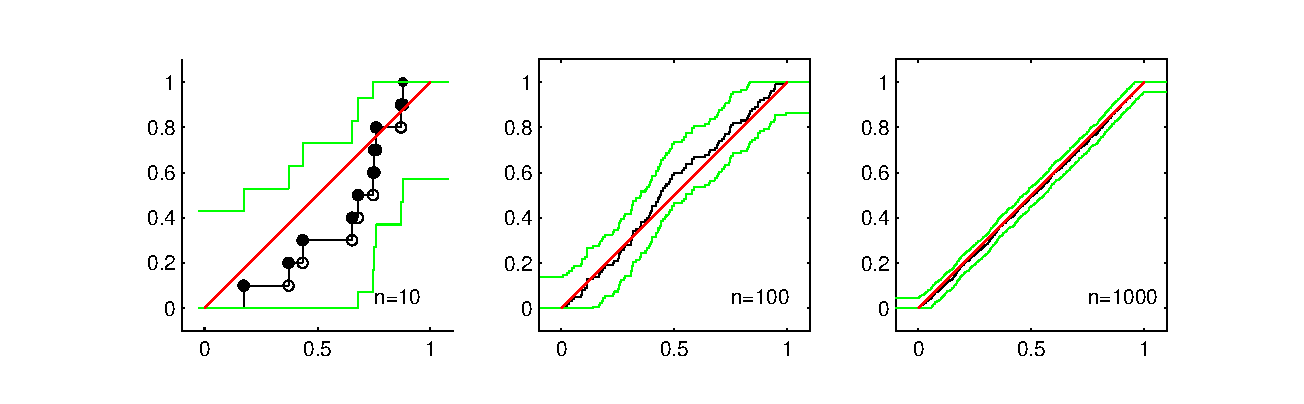
\includegraphics [width=4.25in]{figures/UniformECDFsBands}}
\end{figure}
\vspace{-1.0cm}
\begin{figure}[htpb]
%\centering   \makebox{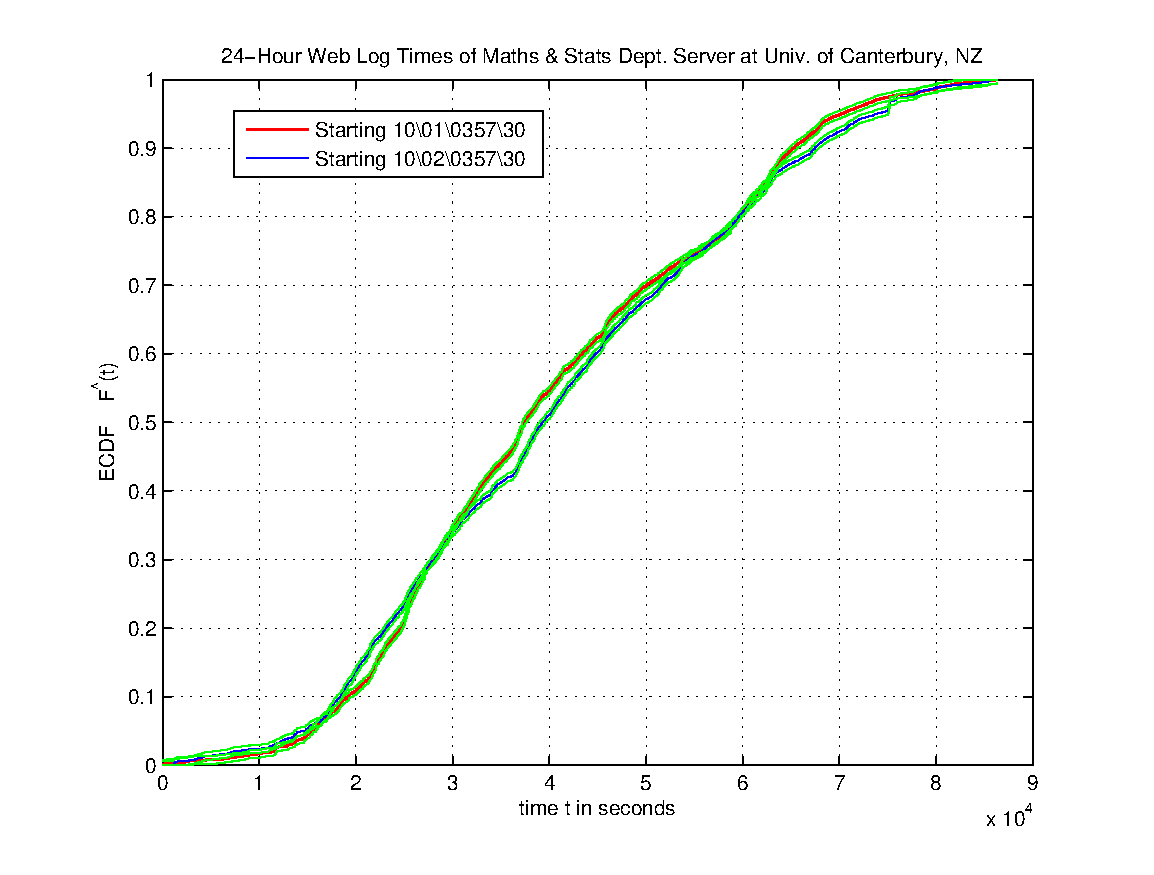
\includegraphics [width=5.0in]{figures/WebLogTimesECDFsBands}}
\centering   \makebox{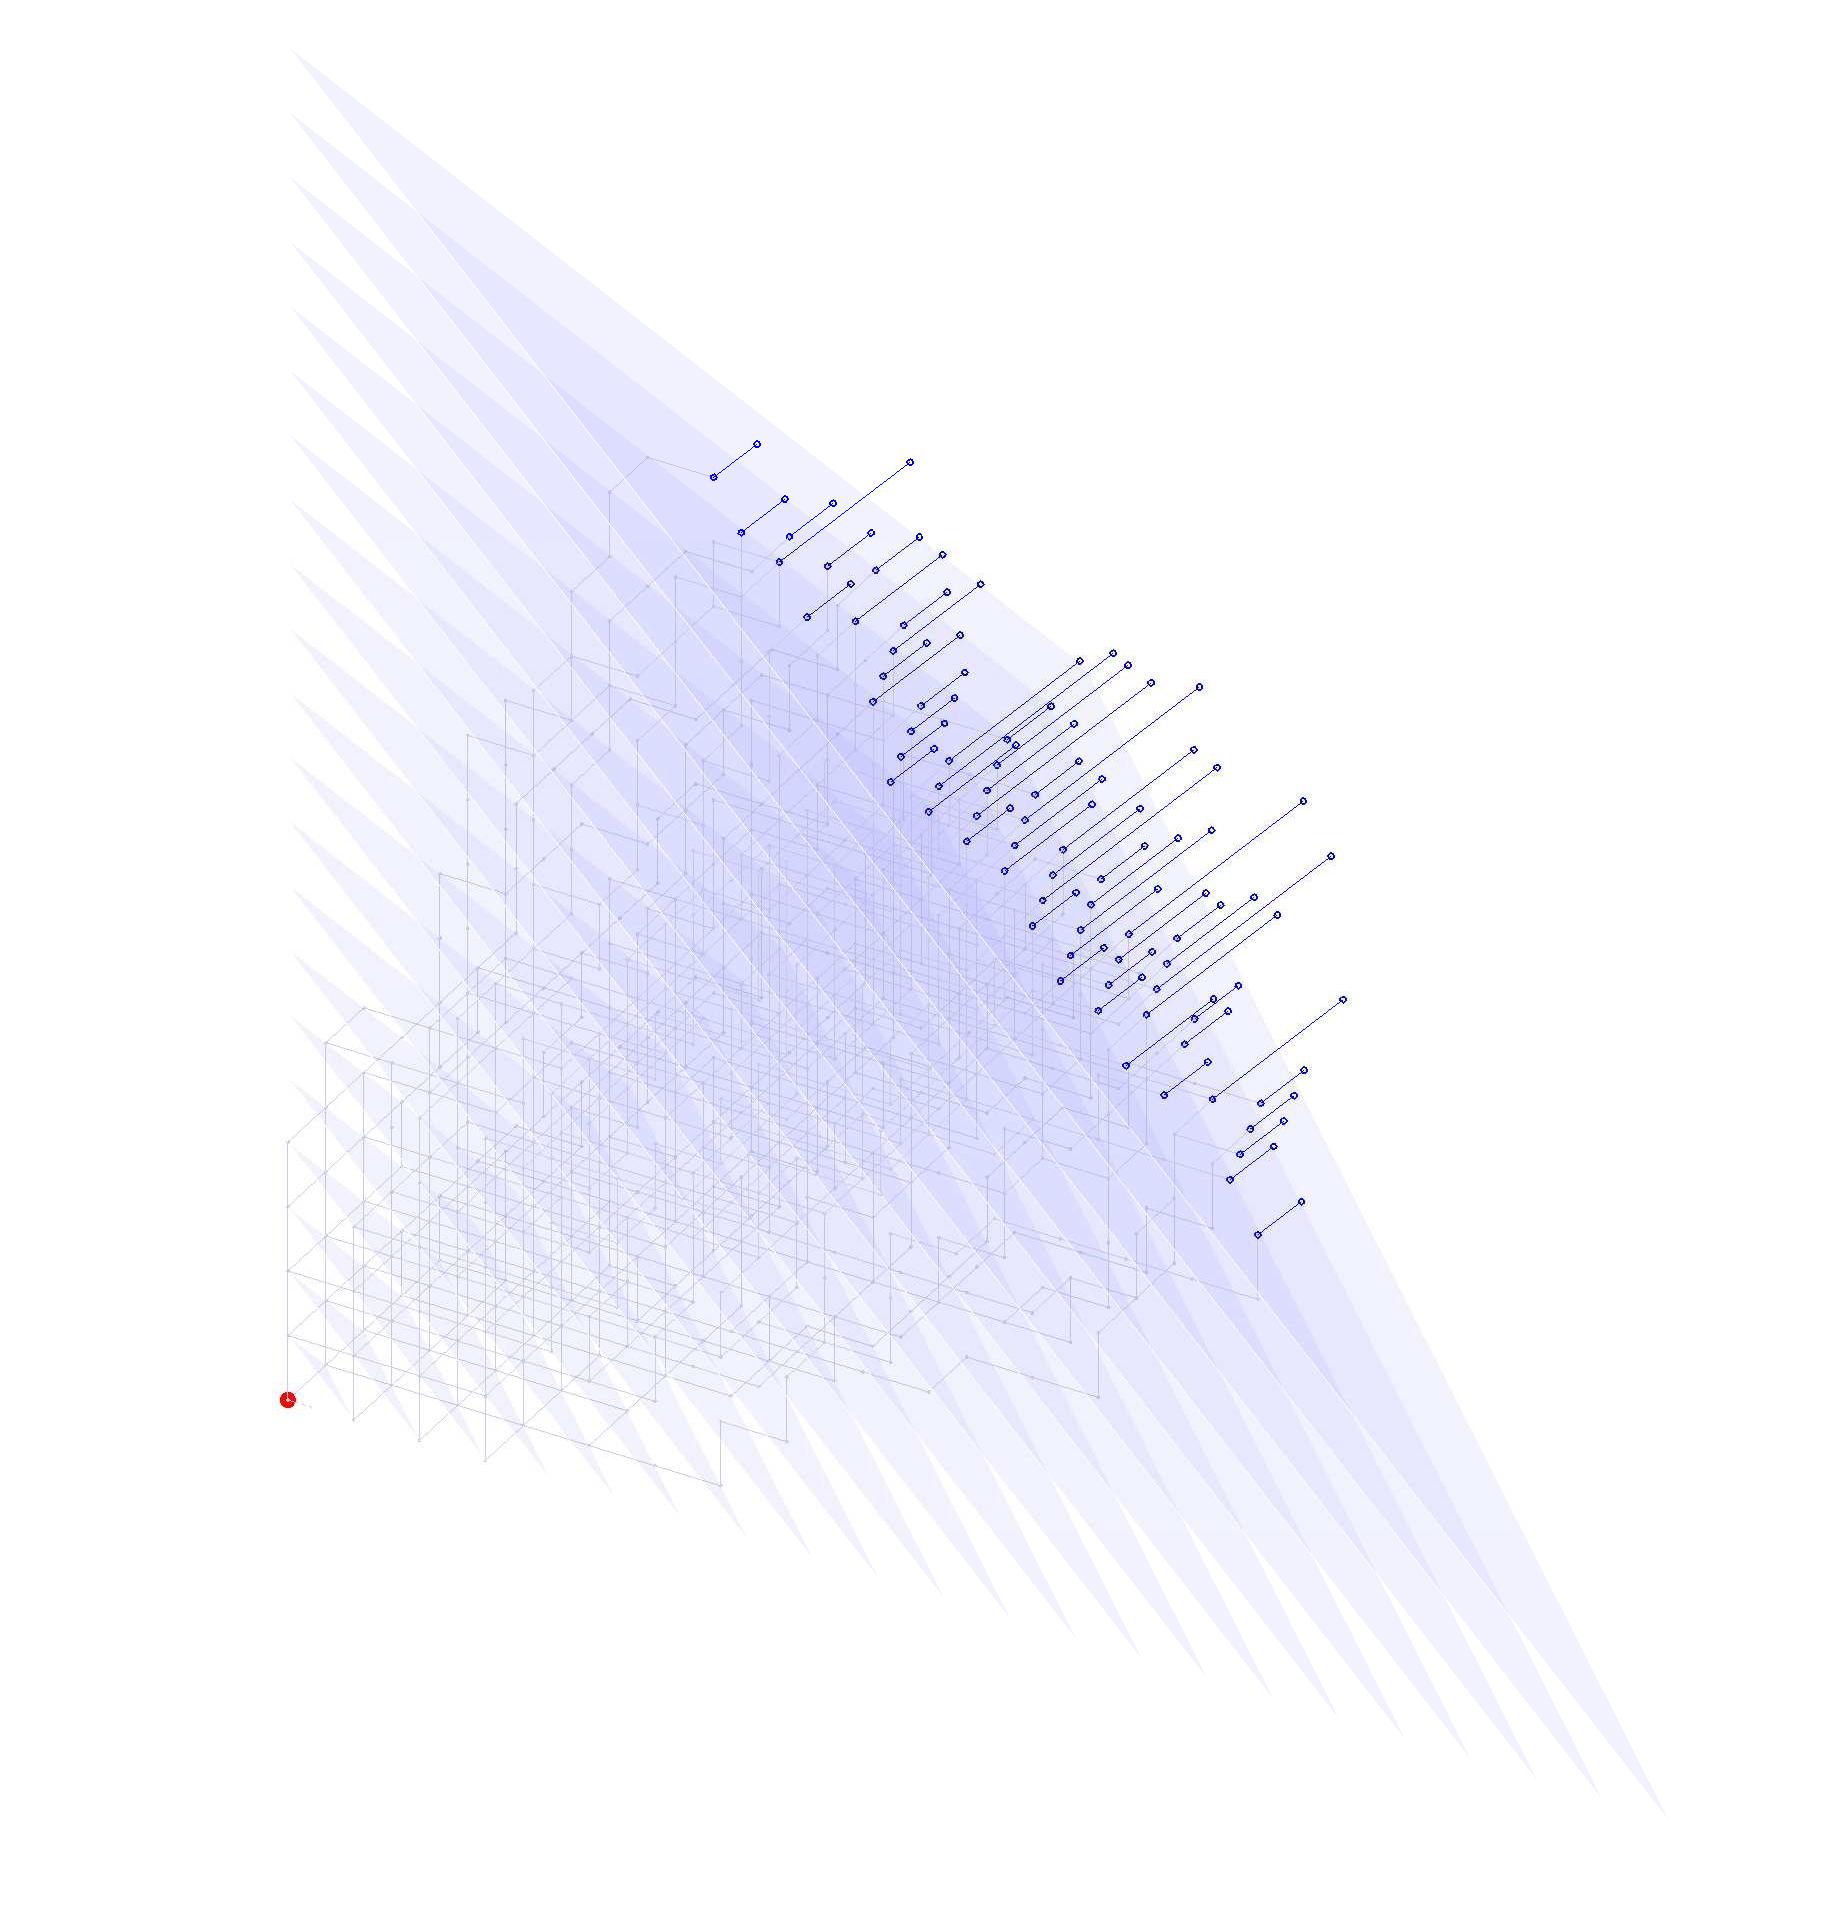
\includegraphics [width=4.5in]{figures/SeptcunxN21T100}}
\end{figure}
}
\maketitle

%\remove{
%\chapter*{Vision Satement}

%\section*{Computational Statistical Experiments in \Matlab}\label{S:CompStatExps}

This book is intended as an undergraduate textbook on introductory to intermediate level Computational Statistics. The goal is to equip students with some of the most useful tools in Computational Statistics and the ability to use them effectively. This will be achieved by maintaining balance between theoretical foundation, algorithmic implementation and practical application of these tools. Hands-on experimentation is encouraged by describing algorithms in pseudocode as well as providing functional and self-contained Matlab code, together with plenty of real data examples. The book will adopt a spiral model of instruction that emphasizes motivation, clarity and concreteness of ideas at the introductory level, followed by mathematical formalism, implementational subtleties and extensions at the intermediate level.

\subsection*{Who is this book addressed to?}
This book is a guide for a {\it computational statistical experimenter}.

A {\it statistical experimenter} is a person who conducts a {\it statistical experiment} (for simplicity, from now on, these will be called ``experimenters" and ``experiments").  Roughly, an experiment is an action with an {\it empirically observable outcome} (data) that cannot necessarily be predicted with certainty, in the sense that a {\it repetition} of the experiment may result in a different outcome.  Most quantitative scientists are experimenters if they apply statistical principles to further their current understanding or {\it theory} of an {\it empirically observable real-world phenomenon} (simply, a {\it phenomenon}).  Roughly, `furthering' your understanding or theory is done by improving your mathematical model (\lq rigorous cartoon\rq) of the phenomenon on the basis of its compatibility with the {\it observed data} or {\it outcome} of the experiment.  In this sense, an experimenter attempts to learn about a phenomenon through the outcome of an experiment.  An experimenter is often a scientist or engineer, and vice versa.

Technological advances have fundamentally inter-twined computers with most experiments today.  First, our instrumentational capacity to observe an empirical phenomenon, by means of automated data gathering (sensing) and representation (storage and retrieval), is steadily increasing.  Second, our computational capability to process statistical information or to make decisions using such massive data-sets is also steadily increasing.  Thus, our recent technological advances are facilitating computationally intensive statistical experiments based on possibly massive amounts of empirical observations, in a manner that was not viable a decade ago.  Hence, a successful scientist or engineer in most specialisations today is a {\it computational statistical experimenter}, i.e.~a statistical experimenter who understands the information structures used to represent their data as well as the statistical algorithms used to process their scientific or engineering decisions.  This course is designed to help you take the first steps along this path.

Let us first demonstrate the need for a statistical experiment.  Recall that statistical inference or learning is the process of using observations or data to infer some aspect of the distribution function (DF) that generated it.  A generic question is:
\[
\text{Given realisations from $X_1, X_2, \ldots, X_n \sim$ some unknown DF $F$, how do we infer $F$} ?
\]
Some of the concrete problems involving experiments include:
\begin{itemize}
\item {\bf Simulation:} Often, it is necessary to simulate a random variable (RV) with some specific distribution to gain insight into its features or simulate whole systems, such as the air-traffic queues at Heathrow Airport, to make better management decisions.
\item {\bf Exploration:} This is the art of (visually) exploring the observed data in order to better understand the empirical phenomenon that generated the data.  Visual explorations of simulated data may provide benchmarks against which we may compare and contrast the observed data.
\item {\bf Estimation:}
\begin{enumerate}
\item {\bf Parametric Estimation:} Using samples from some unknown DF $F$ that is parameterised by some unknown $\theta$, we can estimate $\theta$ from a statistic $\widehat{\Theta}_n$ called the estimator of $\theta$ using one of several methods (maximum likelihood, moment estimation or parametric bootstrap).
\item {\bf Non-parametric Estimation of the DF:}  Based on $n$ independent and identically distributed (IID) observations from an unknown DF $F$, we can estimate it under the general assumption that $F$ belongs to the collection all DFs.
\item {\bf Confidence Sets:}  We can obtain a $1-\alpha$ confidence set for the point estimates, of the unknown parameter $\theta$  that belongs to a collection of parameters (also known as parameter space) denoted by $\BB{\Theta}$ or the unknown  DF $F$ that belongs to the collection all DFs denoted by $\{ \text{all DFs} \}$.
\end{enumerate}
\item {\bf Testing:}  Based on observations from some DF $F$ that is hypothesised as belonging to a subset $\BB{\Theta}_0$ of $\BB{\Theta}$ called the space of null hypotheses, we will learn to test (attempt to reject) the falsifiable null hypothesis that $F$ belongs to a smaller collection of parameters denoted by $\BB{\Theta}_0$.  This smaller collection is contained in the parameter space $\BB{\Theta}$.
\item {\bf Learning:}  Supervised, unsupervised learning, classification and regression \ldots
\end{itemize}

\subsection*{What is unique about our book?}

\begin{itemize}
\item Our unified and integrative approach to statistical experiments where mathematical, statistical and computational aspects naturally come together, will provide the student with the fundamentals so that they can pursue new experiments on their own.
\item Current books in the field either focus on a long list of recipes with little cohesive mathematical and algorithmic structure or ignore fundamental aspects of the field such as the rudiments of random number generation.  Our book is specifically designed to have a solid introduction to the fundamentals in the style of classical books in the foundational areas by Luc Devroye, Donald Knuth and Larry Wasserman.
\item Appealing to students of the YouTube generation is a high priority.  Various measures have been taken to keep the book interesting to the current generation of students.  These measures include:
\begin{itemize}
\item Each concept is introduced from a historical perspective to make it more concrete for the student.
\item Kinesthetic learning --- learning by doing with one's hands --- is known to reinforce mathematical and algorithmic concepts.  We have chosen several experiments that allow kinesthetic learning (Galton's quincunx, Galton's dice, Buffon's Needle, etc.).  See the accompanying Laboratory for Mathematical statistical Experiments and the devices that have been built for such purpose at \url{http://www.math.canterbury.ac.nz/~r.sainudiin/lmse}.
\item Computer animations and interactive visualisations of each fundamental concept is provided with \Matlab code.  The instructor and/or the student may use these code demos to teach and/or learn each concept.
\item Our book uses \Matlab as opposed to {\tt R} for computational statistics.  In most engineering curricula, \Matlab is used in almost all other courses.  Therefore, there is a demand for a book in computational statistics in \Matlab in our increasingly data-rich world.
\item All codes for the book will be provided and no additional toolboxes will be needed.  In effect our codes will form a toolbox that will accompany the book.
\item Our examples are taken from physical, social and biological sciences to keep the subject of interest to computational statistical experimenters across all fields of science and engineering.
\item Finally, the most unique aspect of our book is the student projects.  We encourage each student to conduct her/his own experiment, including the original concept formulation, data collection, algorithm design, coding and data analysis and writing a statistical report. Please visit:
\begin{itemize}
\item
\href{http://www.math.canterbury.ac.nz/~r.sainudiin/courses/STAT218/projects/Stat218StudentProjects2007.pdf}{\url{http://www.math.canterbury.ac.nz/~r.sainudiin/courses/STAT218/projects/Stat218StudentProjects2007.pdf}} \item
\href{http://www.math.canterbury.ac.nz/~r.sainudiin/courses/STAT218/projects/Stat218StudentProjects2008.pdf}{\url{http://www.math.canterbury.ac.nz/~r.sainudiin/courses/STAT218/projects/Stat218StudentProjects2008.pdf}}
\end{itemize}
to see the term projects completed by budding computational statistical experimenters, students of this course at our home institution.
\end{itemize}
\end{itemize}


\section*{Working Outline of Chapters}
The statistical experiment and the basic objects that make it mathematically definitive and internally consistent are introduced later. The precursor to an experiment is a mathematical model for probability in the `real world' called the {\it probability model}.  This arises from an axiomatic system based on more fundamental objects, such as sample space, outcomes, events, probability, the addition rule for mutually exclusive events, the definition of conditional probability, limits, real number system, and random variables.  These objects in turn build on the set theory, so a refresher in set theory is our first stop.  Then, we will introduce the probability model via the intuition behind this construction, and various useful notions associated with continuous and discrete random variables, such as distribution, density, mass function and expectations.  Commonly encountered random variables will serve as examples.  We will learn to simulate these random variables and visualise the realisations.  We will visit the most elementary limit theorems before conducting our own computational statistical experiments involving estimation, testing and learning.

The Table of Contents from a rough set of lecture notes (our starting point for the final book) are attached below.  We hope to have about 500 pages when we are finished with our book.


\chapter*{Course Syllabus and Overview}
\addcontentsline{toc}{chapter}{Course Syllabus}
%\input{styles/SyllabusSTAT218_2008_S2.latex}
%\input{styles/SyllabusSTAT313_2009_S2.tex}
%\input{styles/SyllabusSTAT459.latex}
%\input{styles/SyllabusSTAT313.latex}
\input{styles/ProbTheor1_UU_2019T1.latex}
%}%% end remove

\tableofcontents
\listoftables
\listoffigures

%\chapter{Introduction and Preliminaries}
%Lecture Notes for STAT 313 \& 459 S2 2011: Computational Statistics\\
%Raazesh Sainudiin, Dept.~of Maths \& Stats, University of Canterbury, Christchurch, NZ.


%\remove{
\chapter{Preliminaries}\label{S:Preliminaries}
\section{Elementary Set Theory}\label{S:SetTheory}
A {\bf set} is a collection of distinct objects.  We write a set by enclosing its elements with curly braces.  For example, we denote a set of the two objects $\circ$ and $\bullet$ by:
\[
\boxed{
\{\circ, \bullet\}
} \ .
\]
Sometimes, we give names to sets.  For instance, we might call the first example set $A$ and write:
\[
\boxed{
A=\{\circ, \bullet\} }
\ .
\]
We do not care about the order of elements within a set, i.e.~$A=\{\circ, \bullet\}=\{\bullet,\circ\}$.  We do not allow a set to contain multiple copies of any of its elements unless the copies are distinguishable, say by labels.  So, $B=\{\circ, \bullet, \bullet\}$ is not a set unless the two copies of $\bullet$ in $B$ are labelled or marked to make them distinct, e.g.~$B=\{\circ,\tilde{\bullet},\bullet'\}$.  Names for sets that arise in a mathematical discourse are given upper-case letters ($A,B,C,D,\ldots$).  Special symbols are reserved for commonly encountered sets.

Here is the set $\BB{\E{G}}$ of twenty two Greek lower-case alphabets that we may encounter later:

{\scriptsize
\begin{tabular}{llllllllllllllllllllll}
$\BB{\E{G}} = \{\ \alpha$,& $\beta$,& $\gamma$,& $\delta$,& $\epsilon$,& $\zeta$,& $\eta$,& $\theta$,& $\kappa$,& $\lambda$,& $\mu$,& $\nu$,& $\xi$,& $\pi$,& $\rho$,& $\sigma$,& $\tau$,& $\upsilon$,& $\phi$,& $\chi$,& $\psi$,& $\omega \ \} $
%alpha,& beta,& gamma,& delta,& epsilon,& zeta,& eta,& theta,& kappa,& lambda,& mu,& nu,& xi,& pi,& rho,& sigma,& tau,& upsilon,& phi,& chi,& psi,& omega
\end{tabular} \ .
}

They are respectively named alpha, beta, gamma, delta, epsilon, zeta, eta, theta, kappa, lambda, mu, nu, xi, pi, rho, sigma, tau, upsilon, phi, chi, psi and omega.  $LHS$ and $RHS$ are abbreviations for objects on the Left and Right Hand Sides, respectively, of some binary relation.  By the notation:
\[
\boxed{
LHS := RHS
} \ ,
\]
we mean that $LHS$ {\bf is equal, by definition, to} $RHS$.

The set which does not contain any element (the collection of nothing) is called the {\bf empty set}:
\[
\boxed{
\emptyset := \{ \, \}
} \ .
\]

We say an element $b$ {\bf belongs to} a set $B$, or simply that $b$ belongs to $B$ or that $b$ is an element of $B$, if $b$ is one of the elements that make up the set $B$, and write:
\[
\boxed{
b \in B
} \ .
\]
When $b$ {\bf does not belong to} $B$, we write:
\[
\boxed{
b \notin B
} \ .
\]
For our example set $A = \{\circ, \bullet\}$, $\star \notin A$ but $\bullet \in A$.

We say that a set $C$ is a {\bf subset} of another set $D$ and write:
\[
\boxed{
C \subset D
}
\]
if every element of $C$ is also an element of $D$.  By this definition, any set is a subset of itself.

We say that two sets $C$ and $D$ are {\bf equal} (as sets) and write $C=D$ `if and only if' ($\iff$) every element of $C$ is also an element of $D$, and every element of $D$ is also an element of $C$.  This definition of set equality is notationally summarised as follows:
\[
\boxed{
C=D \quad \iff \quad C \subset D , D \subset C
} \ .
\]
When two sets $C$ and $D$ are not equal by the above definition, we say that $C$ is {\bf not equal} to $D$ and write:
\[
\boxed{
C \neq D
} \ .
\]
The {\bf union} of two sets $C$ and $D$, written as $C \cup D$, is the set of elements that belong to $C$ or $D$.  We can formally express our definition of set union as:
\[
\boxed{
C \cup D := \{x: x \in C \quad \text{or} \quad x\in D \}
} \ .
\]
When a colon ($:$) appears inside a set, it stands for `such that'.  Thus, the above expression is read as `$C$ union $D$ is equal by definition to the set of all elements $x$, such that $x$ belongs to $C$ or $x$ belongs to $D$.'

Similarly, the {\bf intersection} of two sets $C$ and $D$, written as $C \cap D$, is the set of elements that belong to both $C$ and $D$.  Formally:
\[
\boxed{
C \cap D := \{x: x \in C \quad \text{and} \quad x\in D \}
} \ .
\]

{\bf Venn diagrams} are visual aids for set operations as in the diagrams below.

\begin{figure}[htbp]
\centering
%TODO\includegraphics[width=5.5in]{figures/VennDiagsAUbANB.png}
\caption{Union and intersection of sets shown by Venn diagrams}
\end{figure}



The set-difference or {\bf difference} of two sets $C$ and $D$, written as $C \setminus D$, is the set of elements in $C$ that do not belong to $D$.  Formally:
\[
\boxed{
C \setminus D := \{x: x \in C \quad \text{and} \quad x\notin D \}
} \ .
\]
When a universal set, e.g. $U$ is well-defined, the {\bf complement} of a given set $B$ denoted by $B^c$ is the set of all elements of $U$ that don't belong to $B$, i.e.:
\[
\boxed{
B^c := U \setminus B
} \ .
\]
We say two sets $C$ and $D$ are {\bf disjoint} if they have no elements in common, i.e.~$C \cap D = \emptyset$.

By drawing  Venn diagrams,  let us check {\bf De~Morgan's Laws}:

\[
\boxed{
\left(A\cup B\right)^c = A^c \cap B^c \text{  and  } \left( A \cap B \right)^c = A^c \cup B^c
}
\]

\begin{figure}[htbp]
\centering
\mbox{
\subfigure[$\left(A\cup B\right)^c = A^c \cap B^c$]{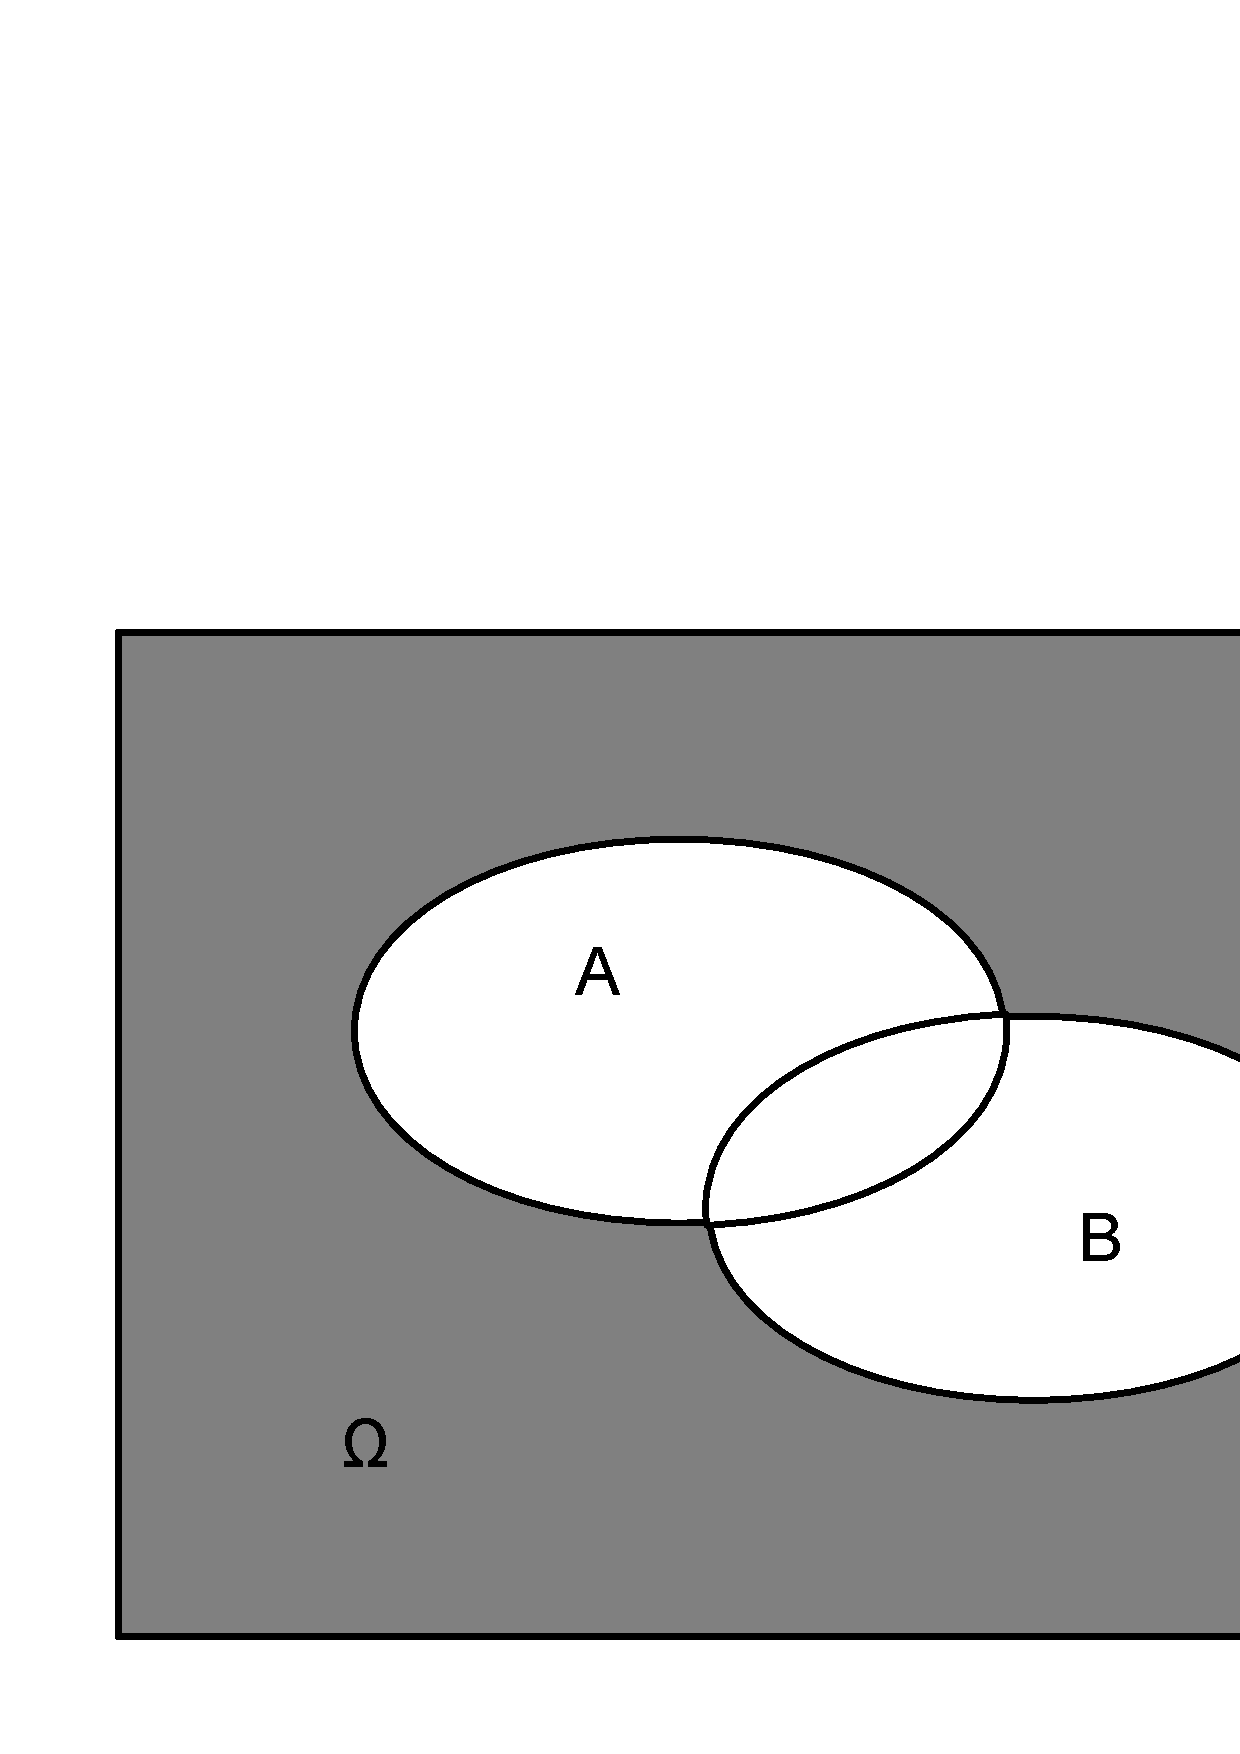
\includegraphics[width=3.0in]{figures/A_union_B_comp}}
\quad
\subfigure[$\left( A \cap B \right)^c = A^c \cup B^c$]{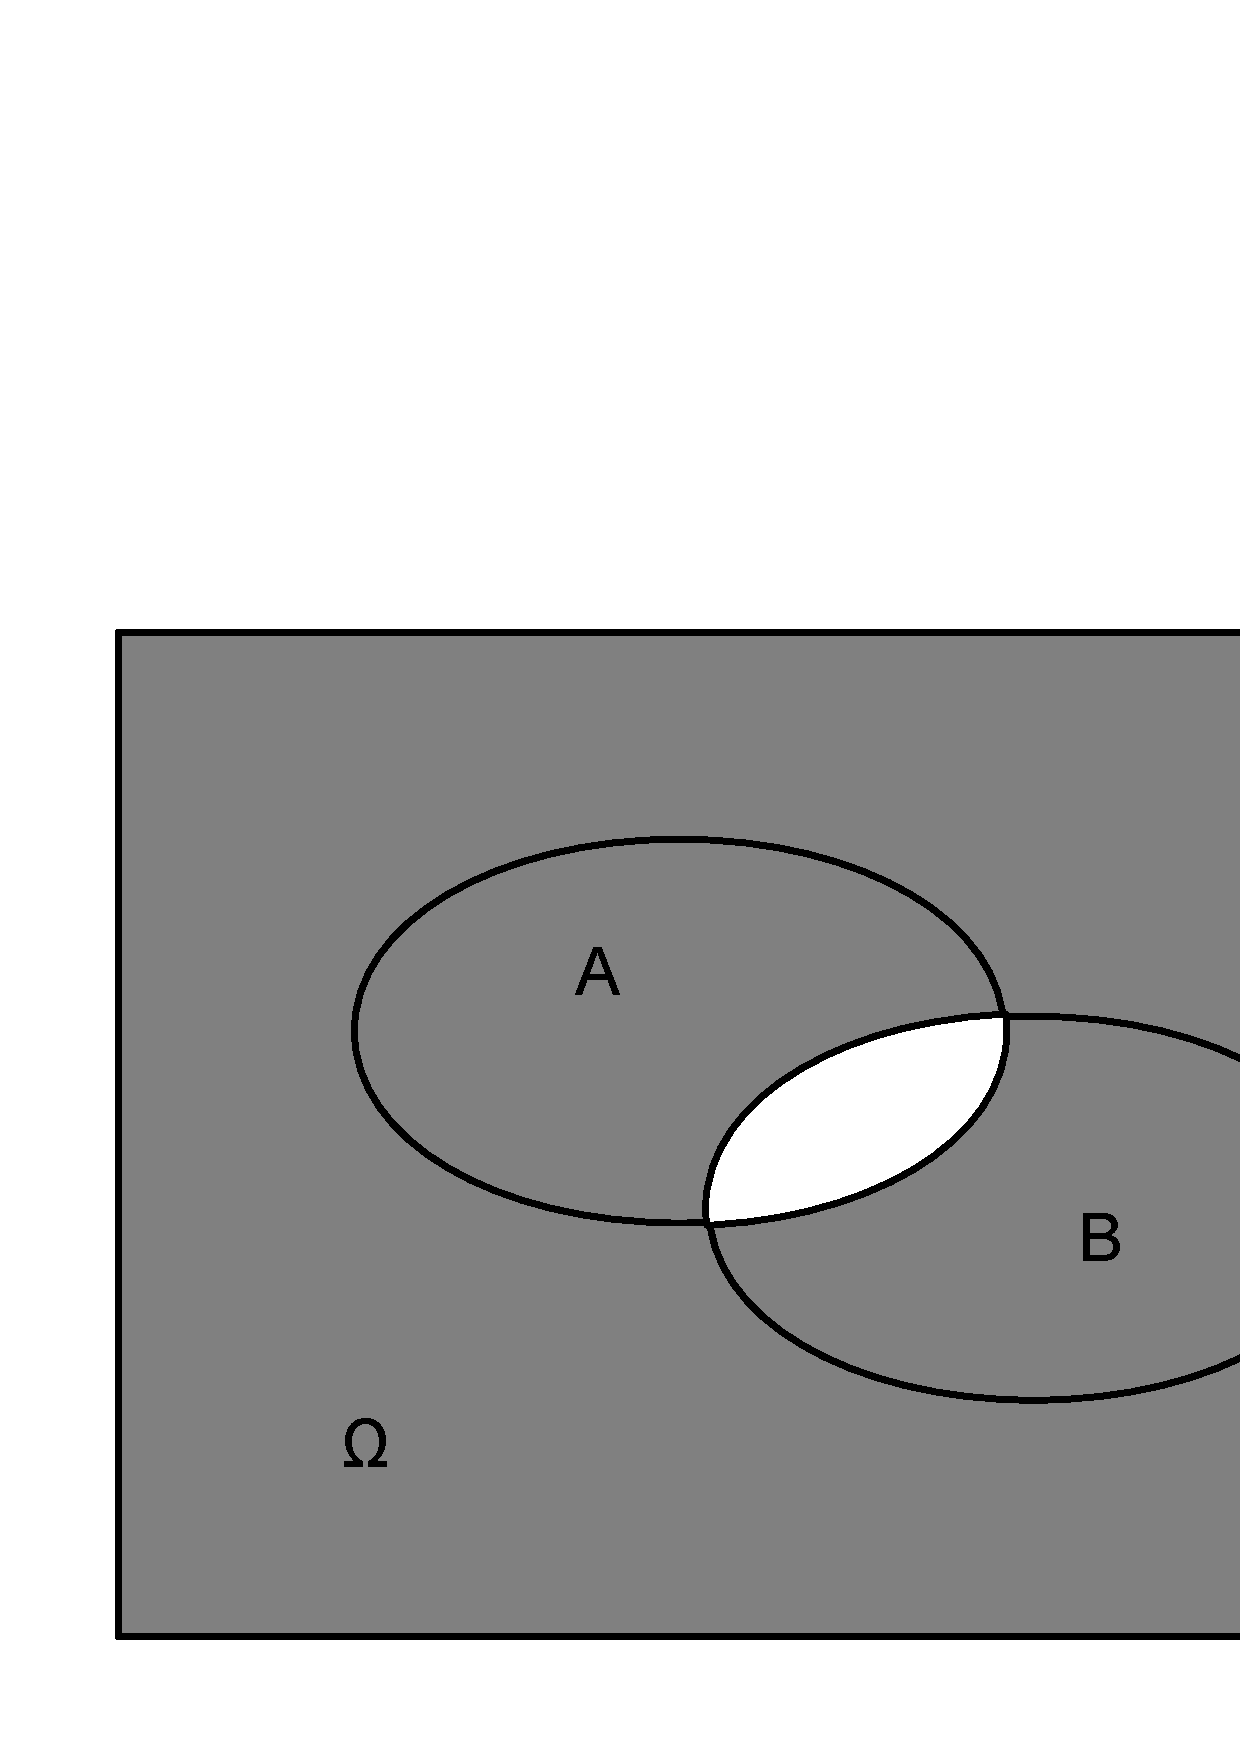
\includegraphics[width=3.0in]{figures/A_inter_B_comp} }
}
\caption{These  Venn diagram illustrate De~Morgan's Laws.} \label{F:DeMorganslaws}
\end{figure}


%\begin{figure}[htpb]
%\caption{Universal set $\Omega$, a set $A$ such that $A \subset \Omega$ (read: $A$ is a subset of $\Omega$ or $A$ is contained in $\Omega$), another set $B$ with $B \subset \Omega$,  the set $A \setminus B$ (read: $A$ (set)minus $B$ or $A$ that is not in $B$), the set $A \cap B$ (read: $A$ intersection $B$), the set $A \cup B$ (read: $A$ union $B$) and the set $A^c$ (read: complement of $A$) which is defined as $\Omega \setminus A$.}
%\vspace{6cm}
%\end{figure}

\begin{classwork}[Fruits and colours]
Consider a set of fruits $F=\{\text{orange}, \text{banana}, \text{apple}\}$ and a set of colours $C = \{\text{red}, \text{green}, \text{blue}, \text{orange}\}$.  Then,
\begin{enumerate}
\item $F \cap C = $
\item $F \cup C = $
\item $F \setminus C = $
\item $C \setminus F = $
\end{enumerate}
\end{classwork}




\begin{classwork}[Subsets of a universal set]
Suppose we are given a universal set $U$, and three of its subsets, $A$, $B$ and $C$.  Also suppose that $A \subset B \subset C$.  Find the circumstances, if any, under which each of the following statements is true (T) and justify your answer:

\begin{tabular*}{5.5in}{@{\extracolsep{\fill}}l l l l}
(1) $C \subset B$ & T when $B=C$
&(2) $A \subset C$ & T by assumption\\
(3) $C \subset \emptyset$ & T when $A=B=C=\emptyset$
&(4) $\emptyset \subset A$& T always \\
(5) $C \subset U$ & T by assumption
&(6) $U \subset A$ & T when $A=B=C=U$\\
\end{tabular*}
\end{classwork}

\section{Exercises}\label{xSets}

\begin{ExerciseList}

\Exercise
Let $\Omega$ be the universal set of students, lecturers and tutors involved in a course.

Now consider the following subsets:
\begin{itemize}
\item The set of 50 students, $S\,=\, \{S_1,\, S_2,\, S_2,\,\dots \, S_{50}\}$.

\item The set of 3 lecturers, $L\,=\, \{L_1,\,L_2,\, L_3\}$.

\item The set of 4 tutors, $T\,=\, \{T_1,\,T_2,\, T_3,\, L_3\}$.
\end{itemize}
Note that one of the lecturers also tutors in the course. Find the following sets:

\bcols{2}\be

\item[(a)] $T \cap L$

\item[(b)] $T \cap S$

\item[(c)] $T \cup L$

\item[(d)] $T \cup L \cup S$

\item[(e)] $S^c$

\item[(f)] $S \cap L$

\item[(g)] $S^c\cap L$

\item[(h)] $T^c$

\item[(i)] $T^c\cap L$


\item[(j)] $T^c\cap T$

\ee\ecols

\Answer
By operating with $\Omega$, $T$, $L$ and $S$ we can obtain the answers as follows:

{\bcols{2}\be

\item[(a)] $T \cap L\,=\, \{L_3\}$

\item[(b)] $T \cap S\,=\, \emptyset$

\item[(c)] $T \cup L\,=\, \{ T_1,\,T_2,\, T_3,\, L_3,\, L_1,\, L_2\}$

\item[(d)] $T \cup L \cup S\,=\, \Omega$

\item[(e)] $S^c \,=\,\{ T_1,\,T_2,\, T_3,\, L_3,\, L_1,\, L_2\} $

\item[(f)] $S \cap L\,=\, \emptyset$

\item[(g)] $S^c\cap L\,=\,\{L_1,\, L_2,\,L_3\}\,=\, L $

\item[(h)] $T^c\,=\,\{L_1,\, L_2,\,S_1,\, S_2,\, S_2,\,\dots \, S_{50}\}  $

\item[(i)] $T^c \cap L\,=\,\{L_1,\, L_2\} $


\item[(j)] $T^c\cap T\,=\, \emptyset$

\ee\ecols
}

%\begin{Exercise}[title={Venn Diagrams 1}]
\Exercise
Using Venn diagram, sketch and check the rule:

$A\cup(B\cap C)\,=\,(A\cup B)\cap (A\cup C)$

\Exercise
Using Venn diagram, sketch and check the rule:

$A\cap(B\cup C)\,=\,(A\cap B)\cup(A\cap C)$

%\end{Exercise}
\Answer
We can check $A\cup(B\cap C)\,=\,(A\cup B)\cap (A\cup C)$ from the following sketch:

\begin{center}
%\subfloat[$A\cup(B\cap C)$]
{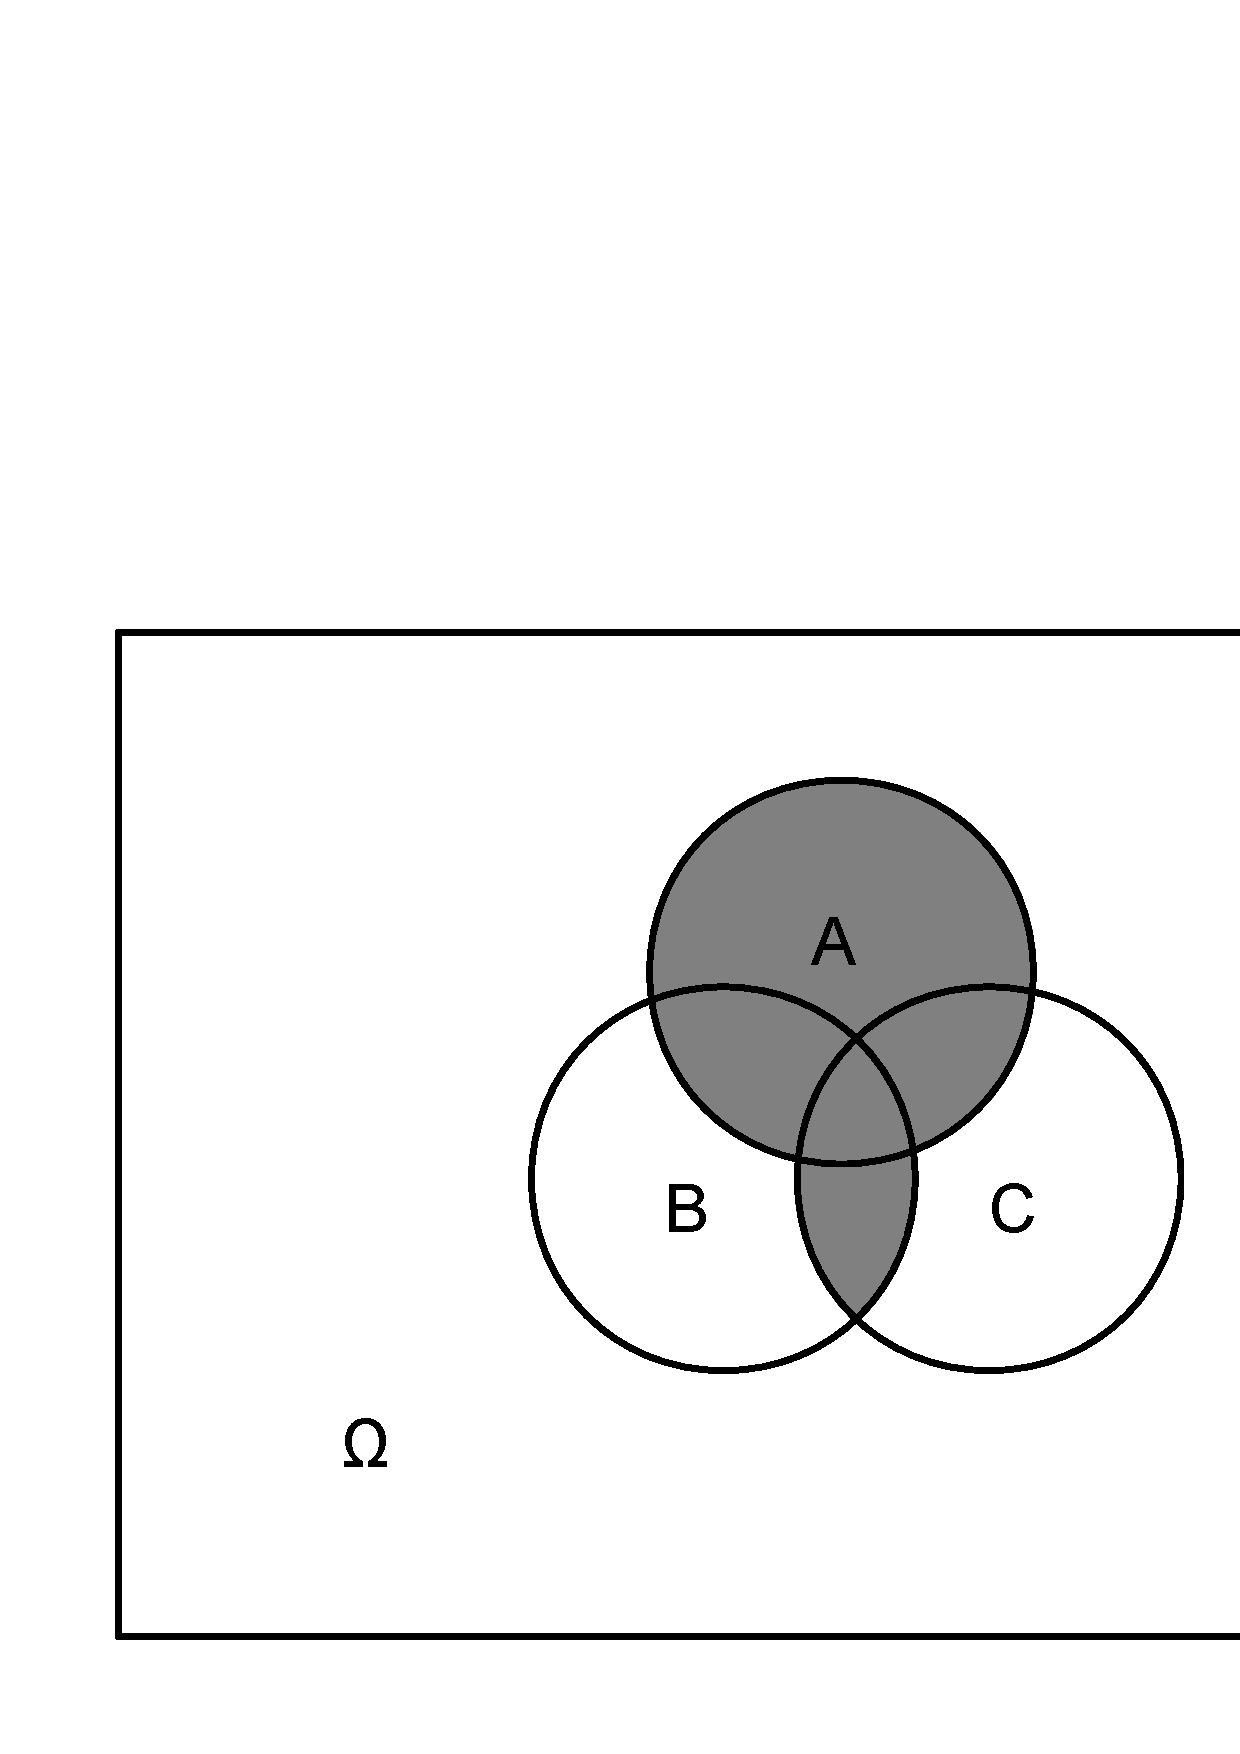
\includegraphics[width=5cm]{figures/ABC1}}
\end{center}

\Answer
We can check $A\cap(B\cup C)\,=\,(A\cap B)\cup(A\cap C)$ from the following sketch:

%\subfloat[$A\cap(B\cup C)$]
We can check $A\cup(B\cap C)\,=\,(A\cup B)\cap (A\cup C)$ from the following sketch:
\begin{center}
{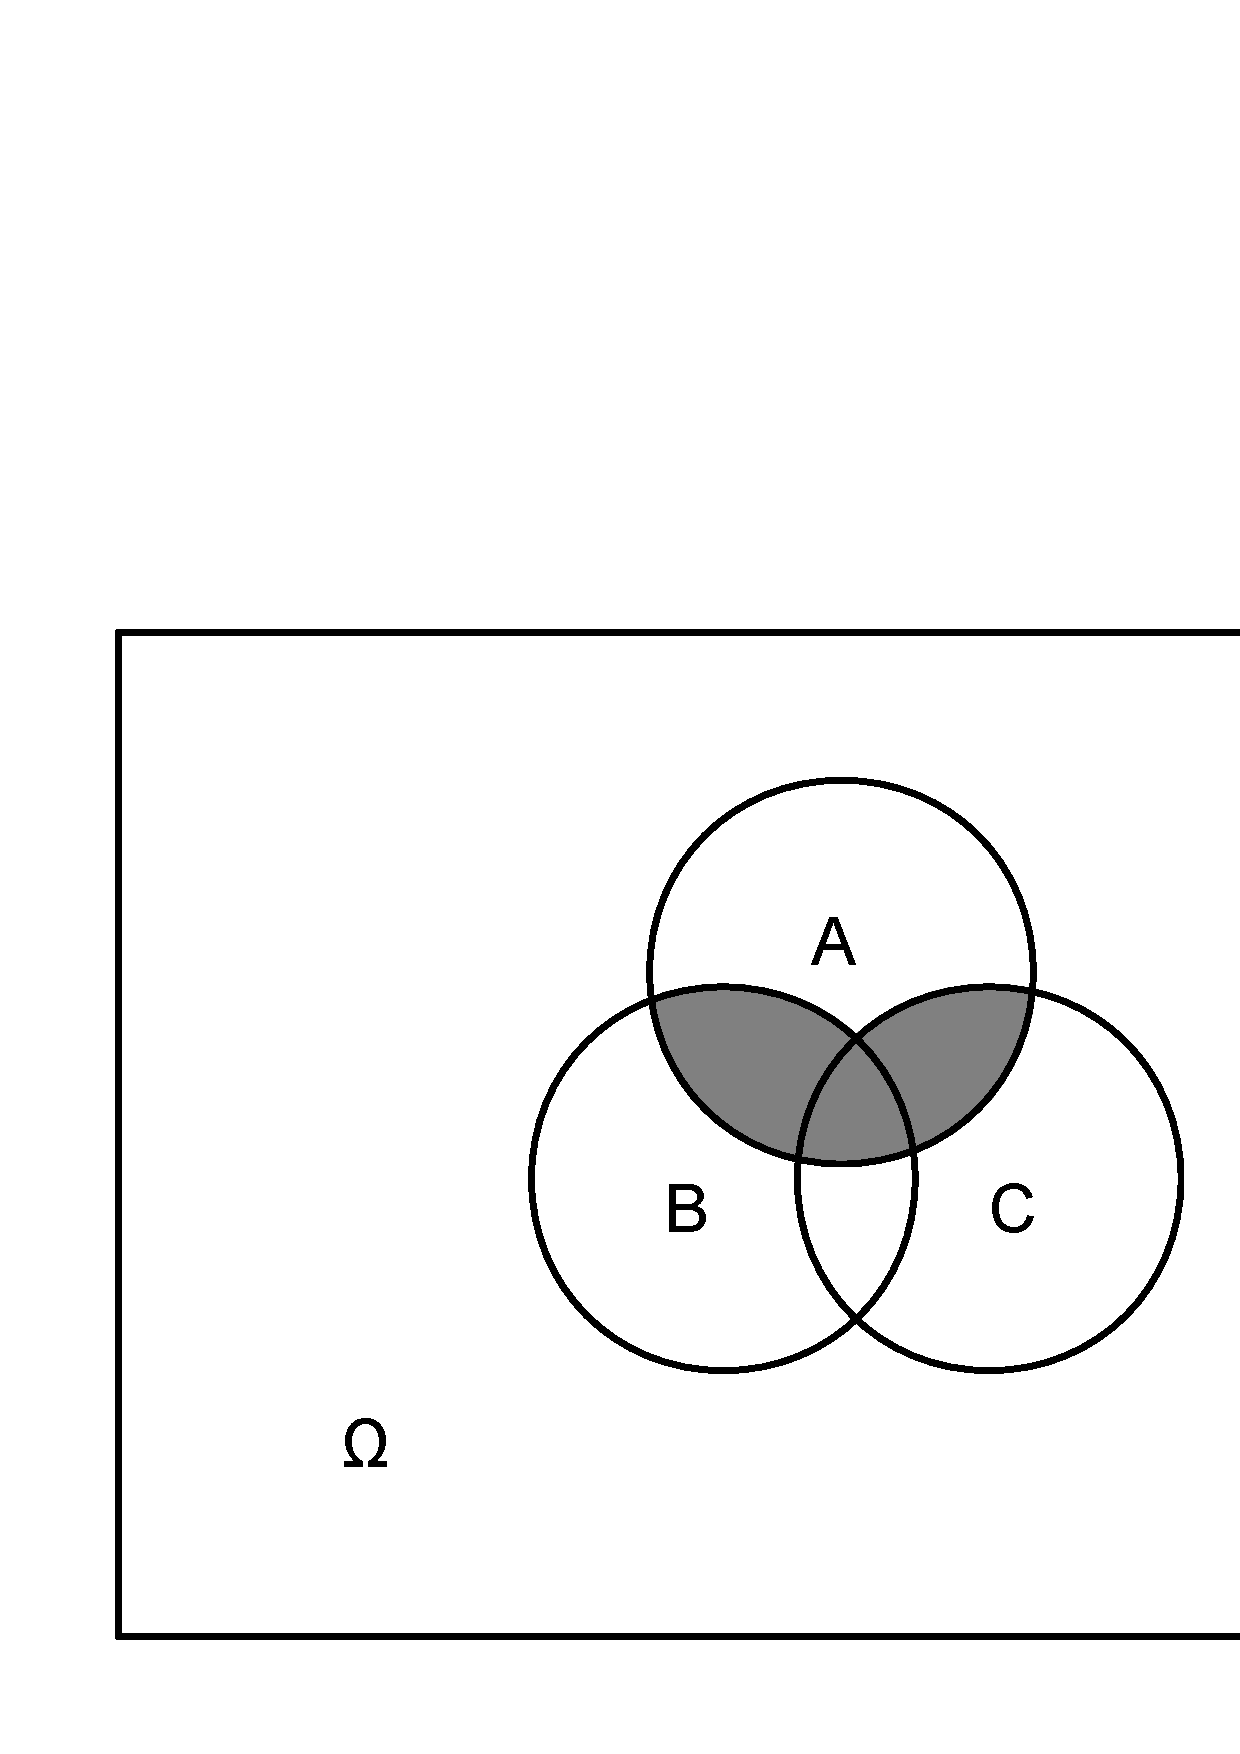
\includegraphics[width=5cm]{figures/ABC2}}
\end{center}

%question 2

%\begin{Exercise}[title={Venn Diagrams 2}]
\Exercise
Using a Venn diagram, illustrate the idea that  $A\subseteq B$ if and only if $A\cup B=B$.
%\end{Exercise}
\Answer
To illustrate the idea that $A\subseteq B$ if and only if $A\cup B=B$, we need to illustrate two implications:
\begin{enumerate}
\item if $A\subseteq B$ then  $A\cup B=B$ and
\item if  $A\cup B=B$ then $A\subseteq B$.
\end{enumerate}
The folowing Venn diagram illustrates the two implications clearly.
\begin{center}
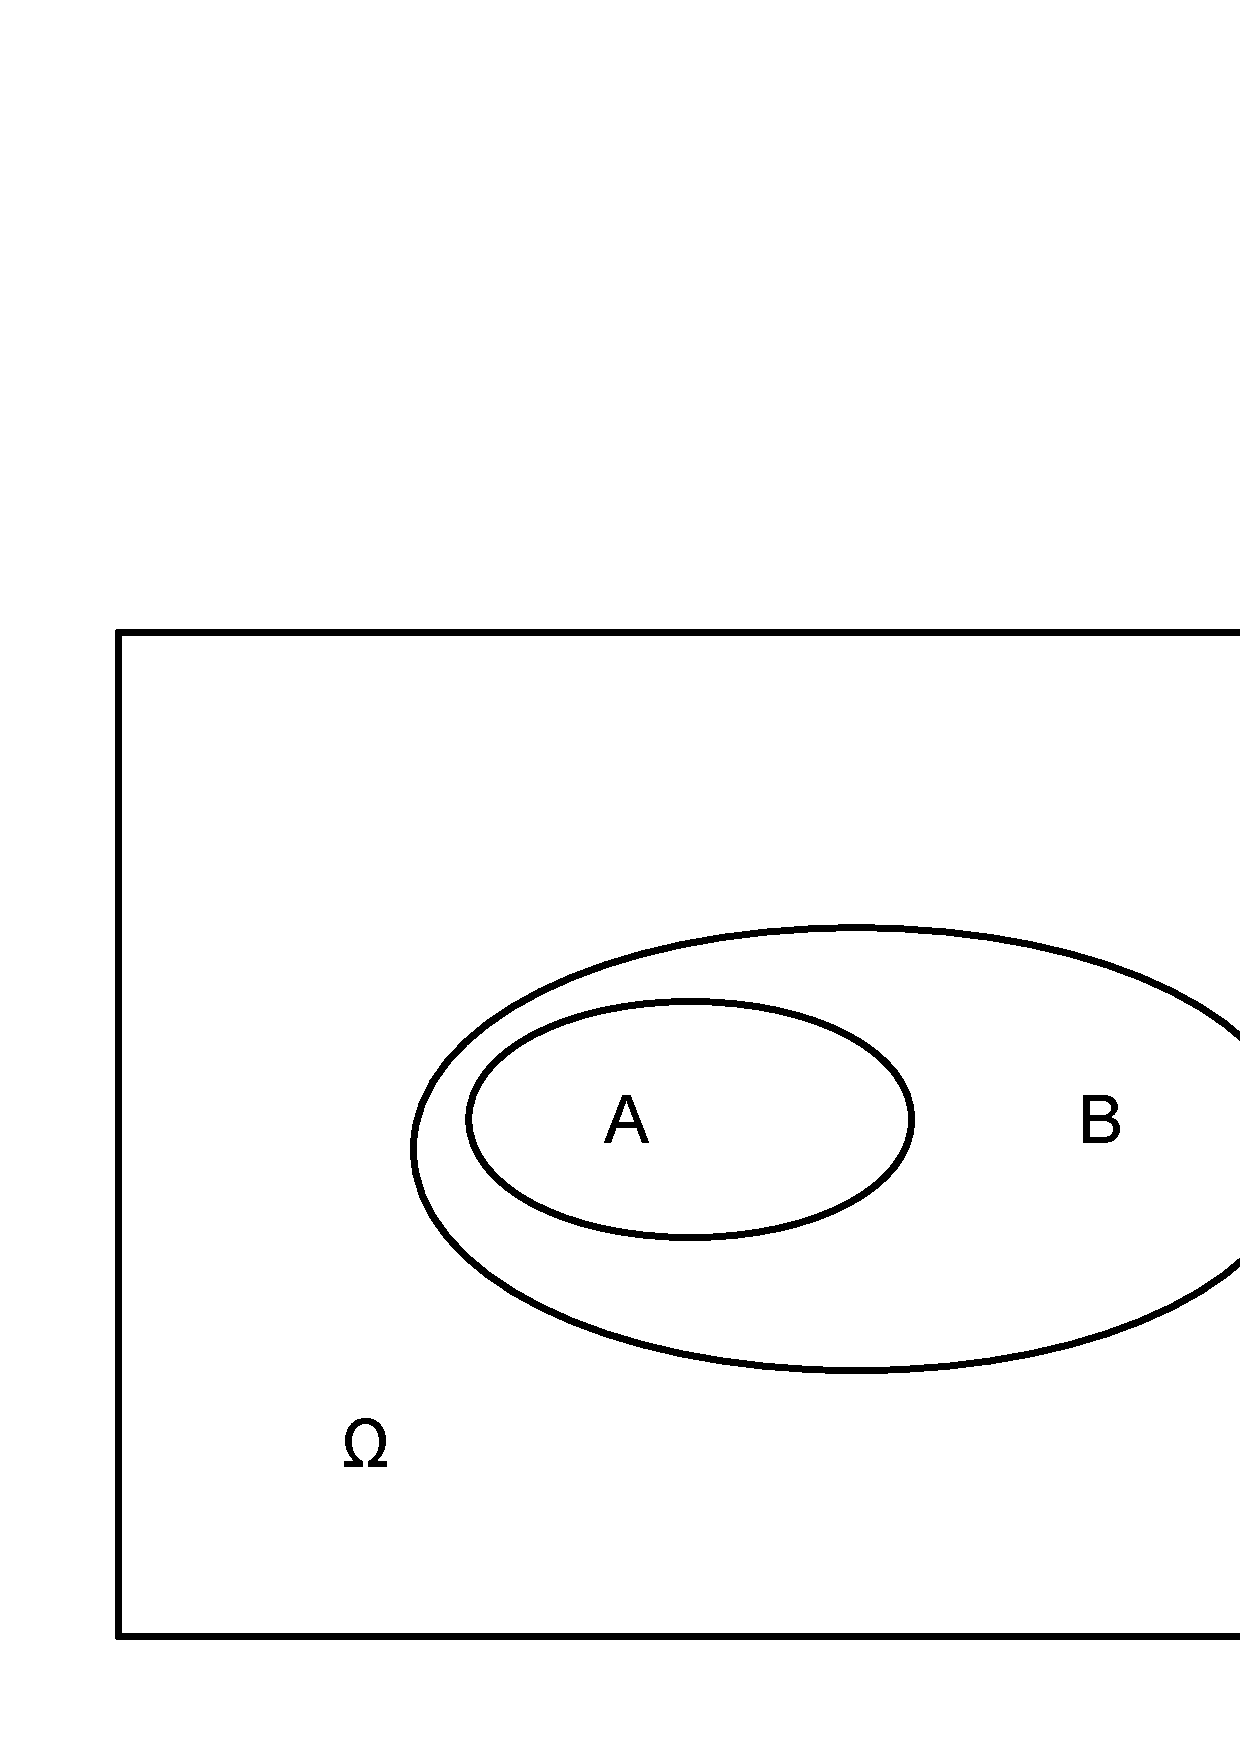
\includegraphics[width=6cm]{figures/AB}
\end{center}

\end{ExerciseList}

\begin{framed}
\begin{tabular}{rcl}
SET SUMMARY\\ \\
$\{a_1,a_2,\dots,a_n\}$& $-$& a set containing the elements, $a_1,a_2,\dots,a_n$.\\
$a\in A$ &$-$& $a$ is an element of the set $A$.\\
$A\subseteq B$ &$-$& the set $A$ is a subset of $B$.\\
$A\cup B$ &$-$& ``union'', meaning the set of all elements which are in $A$ or $B$, \\
& & \ \ or both.\\
$A\cap B$ &$-$& ``intersection'', meaning the set of all elements in both $A$ and $B$.\\
$\{\}$ or $\emptyset$ &$-$& empty set.\\
$\Omega $ &$-$& universal set.  \\
$A^c $ &$-$& the complement of $A$, meaning the set of all elements in $\Omega$,\\
& & \ \ the universal set, which are not in $A$.\\
\end{tabular}
\end{framed}

%\remove{
\section{Natural Numbers, Integers and Rational Numbers}\label{S:NatIntRatNumbers}

We denote the number of elements in a set named $B$ by:
\[
\boxed{
\# B := \text{Number of elements in the set $B$}
} \ .
\]
In fact, the Hindu-Arab numerals we have inherited are based on this intuition of the size of a collection.  The elements of the set of {\bf natural numbers}:
\[
\boxed{
\Nz := \{1,2,3,4,\ldots \}
} \ , \text{may be defined using $\#$ as follows:}
\]
\begin{flalign*}
1 &:= \#\{\star \} = \# \{\bullet\}= \#\{\alpha\}=\#\{\{\bullet\}\} = \#\{\{\bullet,\bullet'\}\}= \ldots,\\
2 &:= \#\{\star',\star \} = \# \{\bullet, \circ\}= \#\{\alpha,\omega\} = \#\{\{\circ\},\{\alpha,\star,\bullet\}\}=\ldots,\\
\vdots &
\end{flalign*}
For our example sets, $A=\{\circ,\bullet\}$ and the set of Greek alphabets $\BB{\E{G}}$, $\# A = 2$ and $\# \BB{\E{G}} = 22$.  The number zero may be defined as the size of an empty set:
\[
0 := \# \emptyset = \#\{\}
\]
The set of {\bf non-negative integers} is:
\[
\boxed{
\Zz_+ := \Nz \cup \{0\} = \{0,1,2,3,\ldots\}
} \ .
\]

A {\bf product set} is the {\bf Cartesian product} ($\times$) of two or more possibly distinct sets:
\[
\boxed{
A \times B := \{(a,b): a \in A \text{ and } b \in B \}
}
\]
For example, if $A=\{\circ,\bullet\}$ and $B=\{\star\}$, then $A\times B = \{(\circ,\star), (\bullet,\star)\}$.  Elements of $A \times B$ are called {\bf ordered pairs}.

The binary arithmetic operation of {\bf addition} ($+$) between a pair of non-negative integers $c,d \in \Zz_+$ can be defined via sizes of disjoint sets.  Suppose, $c=\#C$, $d=\#D$ and $C \cap D = \emptyset$, then:
\[
c+d = \#C + \#D := \# (C \cup D) \ .
\]
For example,  if $A=\{\circ,\bullet\}$ and $B=\{\star\}$, then $A \cap B=\emptyset$ and $\#A + \#B = \#(A \cup B) \iff 2+1=3$.

The binary arithmetic operation of {\bf multiplication} ($\cdot$) between a pair of non-negative integers $c,d \in \Zz_+$ can be defined via sizes of product sets.  Suppose, $c=\#C$, $d=\#D$, then:
\[
c \cdot d = \#C \cdot \#D := \# (C \times D) \ .
\]
For example,  if $A=\{\circ,\bullet\}$ and $B=\{\star\}$, then $\#A \cdot \#B = \#(A \times B) \iff 2 \cdot 1=2$.

More generally, a product set of $A_1,A_2,\ldots,A_m$ is:
\[
\boxed{
A_1 \times A_2 \times \cdots \times A_m := \{(a_1,a_2,\ldots,a_{m}): a_1 \in A_1, a_2 \in A_2, \ldots, a_{m} \in A_m \}
}
\]
Elements of an $m$-product set are called {\bf ordered $m$-tuples}.  When we take the product of the same set we abbreviate as follows:
\[
\boxed{
A^m := \underset{m \text{ times}}{\underbrace{A \times A \times \cdots \times A}} := \{(a_1,a_2,\ldots,a_m): a_1 \in A, a_2 \in A, \ldots, a_{m} \in A \}
}
\]
\begin{classwork}[Cartesian product of sets]
1.~Let $A=\{\circ, \bullet \}$.  What are the elements of $A^2$?  2.~Suppose $\# A = 2$ and $\# B = 3$.  What is $\# (A \times B)$?  3.~Suppose $\# A_1 = s_1, \# A_2 = s_2, \ldots, \# A_m = s_m$.  What is $\# (A_1 \times A_2 \times \cdots \times A_m)$?
\vspace{4cm}
\end{classwork}

Now, let's recall the definition of a function.  A {\bf function} is a ``mapping" that associates each element in some set $\Xz$ (the domain) to exactly one element in some set $\Yz$ (the range). Two different elements in $\Xz$ can be mapped to or associated with the same element in $\Yz$, and not every element in $\Yz$ needs to be mapped.  Suppose $x \in \Xz$. Then we say ${f(x)=y \in \Yz}$ is the {\bf image} of $x$.  To emphasise that $f$ is a {\bf function} from $\Xz \ni x$ to $\Yz \ni y$, we write:
$$\boxed{f(x)=y:\Xz \to \Yz} \ .$$
And for some $y \in \Yz$, we call the set:
$$\boxed{f^{[-1]}(y) := \{x \in \Xz : f(x)=y \} \subset \Xz} \ ,$$
the {\bf pre-image} or {\bf inverse image} of $y$, and
$$\boxed{f^{[-1]} := f^{[-1]}(y \in \Yz) = X \subset \Xz} \ ,$$
as the {\bf inverse} of $f$.

\begin{figure}[htpb]
\caption{A function $f$ (``father of'') from $\Xz$ (a set of children) to $\Yz$ (their fathers) and its inverse (``children of'').\label{F:function}}
\vspace{4cm}
\end{figure}

We motivated the non-negative integers $\Zz_+$ via the size of a set.  With the notion of two directions ($+$ and $-$) and the magnitude of the current position from the origin zero ($0$) of a dynamic entity, we can motivate the set of {\bf integers}:
$$\boxed{\Zz := \{\ldots,-3,-2,-1,0,+1,+2,+3,\ldots\}} \ .$$
The integers with a {\bf minus} or {\bf negative sign} ($-$) before them are called negative integers and those with a {\bf plus} or {\bf positive sign} ($+$) before them are called positive integers.  Conventionally, $+$ signs are dropped.  Some examples of functions you may have encountered are {\bf arithmetic operations} such as {\bf addition} ($+$), {\bf subtraction} ($-$), {\bf multiplication} ($\cdot$) and {\bf division} ($/$) of ordered pairs of integers.  The reader is assumed to be familiar with such arithmetic operations with pairs of integers.  Every integer is either positive, negative, or zero.  In terms of this we define the notion of {\bf order}.  We say an integer $a$ is {\bf less than} an integer $b$ and write $a < b$ if $b-a$ is positive.  We say an integer $a$ is {\bf less than or equal to} an integer $b$ and write $a \leq b$ if $b-a$ is positive or zero.  Finally, we say that $a$ is greater than $b$ and write $a > b$ if $b<a$.  Similarly, $a$ is greater than equal to $b$, i.e.~$a \geq b$, if $b \leq a$.  The set of integers are {\bf well-ordered}, i.e., for every integer $a$ there is a next largest integer $a+1$.

\begin{classwork}[Addition over integers]\label{CW:AdditionMapAndItsInverseMap}
Consider the set of integers $\Zz = \{\ldots,-3,-2,-1,0,1,2,3,\ldots\}$.  Try to set up the arithmetic operation of addition as a function.  The domain for addition is the Cartesian product of $\Zz$:
\[
 \Zz^2 := \Zz \times \Zz := \{(a,b) : a \in \Zz, b \in \Zz \}
\]
What is its range ?
\[
+ : \Zz \times \Zz \to
\]
\begin{figure}[htpb]
\caption{A pictorial depiction of addition and its inverse.  The domain is plotted in orthogonal  {\bf Cartesian coordinates}.\label{F:Addfunction}}
\vspace{5cm}
\end{figure}
\end{classwork}

If the magnitude of the entity's position is measured in units (e.g.~meters) that can be rationally divided into $q$ pieces with $q \in \Nz$, then we have the set of rational numbers:
\[
\Qz := \{ {p}/{q} : p \in \Zz, q \in \Zz \setminus \{0\} \}
\]
The expressions $p/q$ and $p'/q'$ denote the same rational number if and only if $p \cdot q'=p' \cdot q$.  Every rational number has a unique irreducible expression $p/q$, where $q$ is positive and as small as possible.  For example, $1/2$, $2/4$, $3/6$, and $1001/2002$ are different expressions for the same rational number whose irreducible unique expression is $1/2$.

Addition and multiplication are defined for rational numbers by:
\[
\frac{p}{q} + \frac{p'}{q'} = \frac{p \cdot q' + p' \cdot q}{q \cdot q'}
\qquad \text{and} \qquad \frac{p}{q} \cdot \frac{p'}{q'} = \frac{p \cdot p'}{q \cdot q'} \ .
\]
The rational numbers form a {\bf field} under the operations of addition and multiplication defined above in terms of addition and multiplication over integers.  This means that the following properties are satisfied:
\begin{enumerate}
\item Addition and multiplication are each {\bf commutative}
\[ a+b = b+a, \qquad a \cdot b = b \cdot a \ , \]
and associative
\[
a + (b + c) = (a + b) + c, \qquad a \cdot (b \cdot c) = (a \cdot b) \cdot c \ .
\]
\item Multiplication {\bf distributes} over addition
\[
a \cdot (b+c) = (a \cdot b) + (a \cdot c) \ .
\]
\item $0$ is the {\bf additive identity} and $1$ is the multiplicative identity
\[
0+a=a \qquad \text{and} \qquad 1 \cdot a = a \ .
\]
\item Every rational number $a$ has a negative, $a+(-a)=0$ and every non-zero rational number $a$ has a reciprocal, $a \cdot 1/a = 1$.
\end{enumerate}
The field axioms imply the usual laws of arithmetic and allow subtraction and division to be defined in terms of addition and multiplication as follows:
\[
\frac{p}{q} - \frac{p'}{q'} := \frac{p}{q} + \frac{-p'}{q'}
\qquad \text{and} \qquad  \frac{p}{q} / \frac{p'}{q'} := \frac{p}{q} \cdot \frac{q'}{p'}, \quad \text{provided $p' \neq 0$} \ .
\]
We will see later that the theory of finite fields is necessary for the study of pseudo-random number generators (PRNGs) and PRNGs are the heart-beat of randomness and statistics with computers.

%\afterpage{clearpage}

%You should at least have a  ``working knowledge'' of the following topics as they constitute the foundational kernels of statistical reasoning:
%\begin{itemize}
%\item Finite and infinite sequences of rational numbers
%\item Limits, Cauchy sequences of rational numbers and the real number system
%\item Continuous functions, derivatives and differentiable functions
%\end{itemize}
\section{Real Numbers}\label{S:Reals}
Unlike rational numbers which are expressible in their reduced forms by $p/q$, it is fairly tricky to define or express real numbers.  It is possible to define real numbers formally and constructively via equivalence classes of Cauchy sequence of rational numbers.  For this all we need are notions of (1) infinity, (2) sequence of rational numbers and (3) distance between any two rational numbers in an infinite sequence of them.  These are topics usually covered in an introductory course in real analysis and are necessary for a firm  foundation in computational statistics.  Instead of a formal constructive definition of real numbers, we give a more concrete one via decimal expansions.  See Donald E.~Knuth's treatment [{\em Art of Computer Programming, Vol.~I, Fundamental Algorithms}, 3rd Ed., 1997, pp.~21-25] for a fuller story.  A {\bf real number} is a numerical quantity $x$ that has a decimal expansion:
\[
x = n+ 0.d_1d_2d_3 \ldots \ , \text{ where, each } d_i \in \{0,1,\ldots,9\}, n \in \Zz \ ,
\]
and the sequence $ 0.d_1d_2d_3 \ldots$ does not terminate with infinitely many consecutive $9$s.  By the above decimal representation, the following arbitrarily accurate enclosure of the real number $x$ by rational numbers is implied:
\[
n+\frac{d_1}{10}+\frac{d_2}{100}+\cdots+\frac{d_k}{10^k} =: \underline{x}_k \leq x < \overline{x}_k :=
n+\frac{d_1}{10}+\frac{d_2}{100}+\cdots+\frac{d_k}{10^k}+\frac{1}{10^k}
\]
for every $k \in \Nz$.  Thus, rational arithmetic ($+,-,\cdot,/$) can be extended with arbitrary precision to any ordered pair of real numbers $x$ and $y$ by operations on their rational enclosures $\underline{x}, \overline{x}$ and $\underline{y}, \overline{y}$.

Some examples of real numbers that are not rational ({\bf irrational numbers}) are:
\begin{flalign*}
\sqrt{2}=1.41421356237309\ldots & \text{the side length of a square with area of $2$ units}\\
\pi=3.14159265358979\ldots  & \text{the ratio of the circumference to diameter of a circle} \\
e=2.71828182845904\ldots & \text{Euler's constant}
\end{flalign*}
We can think of $\pi$ as being enclosed by the following pairs of rational numbers:
\begin{flalign*}
3 +\frac{1}{10} =: \underline{\pi}_{1} \leq &\pi < \overline{\pi}_{1} := 3 + \frac{1}{10} + \frac{1}{10^{1}} \\
3 +\frac{1}{10} + \frac{4}{100} =: \underline{\pi}_{2} \leq &\pi < \overline{\pi}_{2} := 3 + \frac{1}{10} + \frac{4}{100}+\frac{1}{100} \\
3 +\frac{1}{10} + \frac{4}{100} + \frac{1}{10^3} =: \underline{\pi}_{3} \leq &\pi < \overline{\pi}_{3} := 3 + \frac{1}{10} + \frac{4}{100}+ \frac{1}{10^3}+\frac{1}{10^3} \\
&\vdots \\
3.14159265358979 =: \underline{\pi}_{14} \leq &\pi < \overline{\pi}_{14} := 3.14159265358979 + \frac{1}{10^{14}} \\
& \vdots
\end{flalign*}

Think of the real number system as the continuum of points that make up a line, as shown in ~\hyperref[F:linesegment]{Figure~\ref*{F:linesegment}}.
\begin{figure}[htpb]
\caption{A depiction of the real line segment $[-10,10]$.\label{F:linesegment}}
\vspace{3cm}
\end{figure}

Let $y$ and $z$ be two real numbers such that $y \leq z$.  Then, the {\bf closed interval} $[y,z]$ is the set of real numbers $x$ such that $y \leq x \leq z$:
\[
[y,z] := \{ x: y \leq x \leq z \} \ .
\]
The {\bf half-open interval} $(y,z]$ or $[y,z)$ and the {\bf open interval} $(y,z)$  are defined analogously:
\begin{flalign*}
(y,z] &:= \{ x: y < x \leq z \} \ , \\
[y,z) &:= \{ x: y \leq x < z \} \ , \\
(y,z) &:=  \{ x: y < x < z \} \ .
\end{flalign*}
We also allow $y$ to be {\bf minus infinity} (denoted $-\infty$) or $z$ to be {\bf infinity} (denoted $\infty$) at an open endpoint of an interval, meaning that there is no lower or upper bound.  With this allowance we get the set of {\bf real numbers} $\Rz := (-\infty,\infty)$, the {\bf non-negative real numbers} $\Rz_+:=[0,\infty)$ and the {\bf positive real numbers} $\Rz_{>0}(0,\infty)$ as follows:
\begin{flalign*}
\Rz &:= (-\infty,\infty) =  \{ x: -\infty < x < \infty \} \ , \\
\Rz_+ &:= [0,\infty) =  \{ x: 0 \leq x < \infty \} \ , \\
\Rz_{>0} &:= [0,\infty) =  \{ x: 0 < x < \infty \} \ . \\
\end{flalign*}
For a positive real number $b \in \Rz_{>0}$ and an integer $n \in \Zz$, the $n$-th {\bf power} or {\bf exponent} of $b$ is:
\[
b^0=1, \qquad b^n = b^{n-1} \cdot b \quad \text{if $n>0$}, \qquad b^n=b^{n+1}/b  \quad \text{if $n<0$} \ .
\]
The following {\bf laws of exponents} hold by mathematical induction when $m,n \in \Zz$:
\[
b^{m+n} = b^m \cdot b^n, \qquad \left( b^m \right)^n = b^{m \cdot n} \ .
\]
If $y \in \Rz$ and $m \in \Nz$, the unique positive real number $z \in \Rz_{>0}$ such that $z^m=y$ is called the {\bf $m$-th root of $y$} and denoted by $\sqrt[m]{y}$, i.e.,
\[
z^m=y \implies z=\sqrt[m]{y} \ .
\]
For a rational number $r=p/q \in \Qz$, we define the $r$-th power of $b \in \Rz$ as follows:
\[
b^r = b^{p/q} := \sqrt[q]{b^p}
\]
The laws of exponents hold for this definition and different expressions for the same rational number $r=ap/aq$ yield the same power, i.e.,~$ b^{p/q}= b^{ap/aq}$.  Recall that a real number $x=n+ 0.d_1d_2d_3\ldots \in \Rz$ can be arbitrarily precisely enclosed by the rational numbers $\underline{x}_k:=n+\frac{d_1}{10}+\frac{d_2}{100}+\cdots+\frac{d_k}{10^k}$ and $\overline{x}_k:=n+\frac{d_1}{10}+\frac{d_2}{100}+\cdots+\frac{d_k}{10^k}+\frac{1}{10^k}$ by increasing $k$.  Suppose first that $b>1$.  Then, using rational powers, we can enclose $b^x$,
\[
b^{n+\frac{d_1}{10}+\frac{d_2}{100}+\cdots+\frac{d_k}{10^k}} =: b^{\underline{x}_k} \leq b^{x} < b^{\overline{x}_k} := b^{n+\frac{d_1}{10}+\frac{d_2}{100}+\cdots+\frac{d_k}{10^k}+\frac{1}{10^k}} \ ,
\]
within an interval of width $b^{n+\frac{d_1}{10}+\frac{d_2}{100}+\cdots+\frac{d_k}{10^k}} \left(b^{\frac{1}{10^k}}-1 \right) < b^{n+1}(b-1)/10^k$.  By taking a large enough $k$ we can evaluate $b^x$ to any accuracy.  Finally, when $b<1$ we define $b^x : = (1/b)^x$ and when $b=0$, $b^x := 1$.

Suppose $y \in \Rz_{>0}$ and $b \in \Rz \setminus \{1\}$ then the real number $x$ such that $y=b^x$ is called the {\bf logarithm of $y$ to the base $b$} and we write this as:
\[
y=b^x \iff x = \log_b{y}
\]
The definition implies:
\[
x = \log_b (b^x) = b^{\log_b x} \ ,
\]
and the laws of exponents imply:
\begin{flalign*}
\log_b(xy) &= \log_b{x} + \log_b{y}, \quad \text{if} \quad x >0, \ y >0 \ \text{ and} \\
\log_b \left( c^y \right) &= y \log_b c, \quad \text{if} \quad c > 0 \ .
\end{flalign*}
The {\bf common logarithm} is $\log_{10}(y)$, the {\bf binary logarithm} is $\log_2(y)$ and the {\bf natural logarithm} is $\log_e(y)$, where $e$ is the Euler's constant.  Since we will mostly work with $\log_e(y)$ we use $\log(y)$ to mean $\log_e(y)$.  You are assumed to be familiar with trigonometric functions ($\sin(x)$, $\cos(x)$, $\tan(x)$, $\ldots$).  We sometimes denote the special power function $e^y$ by $\exp(y)$.

Familiar extremal elements of a set of real numbers, say $A$, are the following:
\[
\boxed{
\max{A} := \text{greatest element in $A$}
}
\]
For example, $\max \{1,4,-9,345\} = 345$, $\max [-93.8889,1002.786] = 1002.786$.
\[
\boxed{
\min{A} := \text{least element in $A$}
}
\]
For example, $\min \{1,4,-9,345\} = -9$, $\min [-93.8889,1002.786] = -93.8889$.  We need a slightly more sophisticated notion for the extremal elements of a set $A$ that may not belong to $A$.  We say that a real number $x$ is a {\bf lower bound} for a non-empty set of real numbers $A$, provided $x \leq a$ for every $a \in A$.  We say that the set $A$ is {\bf bounded below} if it has at least one lower bound.  A lower bound is the {\bf greatest lower bound} if it is at least as large as any other lower bound.  The greatest lower bound of a set of real numbers $A$ is called the {\bf infimum} of $A$ and is denoted by:
\[
\boxed{
\inf{A} := \text{greatest lower bound of $A$}
}
\]
For example, $\inf (0,1) = 0$ and $\inf \{ 10.333 \cup [-99,1001.33) \} = -99$.  We similarly define the {\bf least upper bound} of a non-empty set of real numbers $A$ to be the {\bf supremum} of $A$ and denote it as:
\[
\boxed{
\sup{A} := \text{least upper bound of $A$}
}
\]
For example, $\sup (0,1) = 1$ and $\sup \{ 10.333 \cup [-99,1001.33) \} = 1001.33$.  By convention, we define $\inf \emptyset := \infty$, $\sup \emptyset := - \infty$.  Finally, if a set $A$ is not bounded below then $\inf A := - \infty$ and if a set $A$ is not bounded above then $\sup A := \infty$.
\begin{table}[htb]
\centering
{\small
\begin{tabular}{| l | l |}
\hline
Symbol & Meaning\\ \hline
$A = \{ \star, \circ, \bullet \}$& $A$ is a set containing the elements $\star$, $\circ$ and $\bullet$ \\
$\circ \in A$ & $\circ$ belongs to $A$ or $\circ$ is an element of $A$\\
$A \ni \circ$ & $\circ$ belongs to $A$ or $\circ$ is an element of $A$\\
$\odot \notin A$& $\odot$ does not belong to $A$ \\
$\# A$& Size of the set $A$, for e.g.~$\#\{ \star, \circ, \bullet, \odot \}=4$\\
$\Nz$& The set of natural numbers $\{1,2,3,\ldots\}$\\
$\Zz$&The set of integers $\{\ldots,-3,-2,-1,0,1,2,3,\ldots\}$\\
$\Zz_+$& The set of non-negative integers $\{0,1,2,3,\ldots\}$\\
%$\Rz$& The set of real numbers\\
$\emptyset$&Empty set or the collection of nothing or $\{\}$\\
$A \subset B$ & $A$ is a subset of $B$ or $A$ is contained by $B$, e.g.~$A=\{\circ\}, B=\{\bullet\}$\\
$A \supset B$& $A$ is a superset of $B$ or $A$ contains $B$ e.g.~$A=\{\circ, \star,\bullet\}, B=\{\circ, \bullet\}$ \\
$A=B$ & $A$ equals $B$, i.e.~$A \subset B$ and  $B \subset A$\\
$Q \implies R$ & Statement $Q$ implies statement $R$ or If $Q$ then $R$ \\
$Q \iff R$ & $Q \implies R$ and $R \implies Q$ \\
$\{x: x \text{ satisfies property } R \}$& The set of all $x$ such that $x$ satisfies property $R$\\
$A \cup B$& $A$ union $B$, i.e.~$\{x: x\in A \text{ or } x \in B\}$\\
$A \cap B$& $A$ intersection $B$, i.e.~$\{x: x\in A \text{ and } x \in B\}$\\
$A \setminus B $& $A$ minus $B$, i.e.~$\{x: x\in A \text{ and } x \notin B\}$\\
$A:=B$& $A$ is equal to $B$ by definition\\
$A=:B$& $B$ is equal to $A$ by definition\\
$A^c$& $A$ complement, i.e.~$\{x: x\in U, \text{ the universal set, but } x \notin A\}$\\
$A_1 \times A_2 \times \cdots \times A_m$ & The $m$-product set $\{(a_1,a_2,\ldots,a_{m}): a_1 \in A_1, a_2 \in A_2, \ldots, a_{m} \in A_m \}$ \\
$A^m$ & The $m$-product set $\{(a_1,a_2,\ldots,a_{m}): a_1 \in A, a_2 \in A, \ldots, a_{m} \in A \}$ \\
$f := f(x)=y:\Xz \to \Yz$ & A function $f$ from domain $\Xz$ to range $\Yz$ \\
$f^{[-1]}(y)$ & Inverse image of $y$ \\
$f^{[-1]} := f^{[-1]}(y \in \Yz) = X \subset \Xz$ & Inverse of $f$ \\
%$\Zz:=\{\ldots,-2,-1,0,1,2,\ldots\}$ & Integers \\
$a<b$ or $a \leq b$ & $a$ is less than $b$ or $a$ is less than or equal to $b$ \\
$a>b$ or $a \geq b$ & $a$ is greater than $b$ or $a$ is greater than or equal to $b$ \\
$\Qz$ & Rational numbers \\
$(x,y)$ & the open interval $(x,y)$, i.e.~$\{r: x < r < y\}$ \\
$[x,y]$ & the closed interval $(x,y)$, i.e.~$\{r: x \leq r \leq y\}$ \\
$(x,y]$ & the half-open interval $(x,y]$, i.e.~$\{r: x < r \leq y\}$ \\
$[x,y)$ & the half-open interval $[x,y)$, i.e.~$\{r: x \leq r < y\}$ \\
$\Rz := (-\infty,\infty)$ & Real numbers, i.e.~$\{r: -\infty < r <  \infty \}$ \\
$\Rz_+ := [0,\infty)$ & Real numbers, i.e.~$\{r: 0 \leq r <  \infty \}$ \\
$\Rz_{>0} := (0,\infty)$ & Real numbers, i.e.~$\{r: 0 < r <  \infty \}$ \\
\hline
\end{tabular}
}
\caption{Symbol Table: Sets and Numbers \label{T:SymbTableSets}}
\end{table}

\clearpage

\section{Introduction to \Matlab}\label{S:IntroMatlab}
We use \Matlab to perform computations and visualisations. \Matlab is a numerical computing environment and programming language that is optimised for vector and matrix processing.  STAT 218/313 students will have access to Maths \& Stats Department's computers that are licensed to run \Matlab.  You can remotely connect to these machines from home by following instructions at \href{http://www.math.canterbury.ac.nz/php/resources/compdocs/remote}{\url{http://www.math.canterbury.ac.nz/php/resources/compdocs/remote}}.

%\input{LabWeek1.tex}

\begin{labwork}[Basics of \Matlab]\label{LW:IntroMatlab}
Let us familiarize ourselves with \Matlab in this session.  First, you need to launch \Matlab from your terminal.  Since this is system dependent, ask your tutor for help.  The command window within the \Matlab window is where you need to type commands.  Here is a minimal set of commands you need to familiarize yourself with in this session.
\begin{enumerate}
\item{
Type the following command to add 2 numbers in the command window right after the command prompt {\tt >> }.
\begin{VrbM}
>> 13+24
\end{VrbM}
Upon hitting {\tt Enter} or {\tt Return} on your keyboard, you should see:
\begin{VrbM}

ans =

    37

\end{VrbM}
The summand 37 of 13 and 24 is stored in the default variable called {\tt ans} which is short for answer.
}
\item{
We can write {\bf comments} in \Matlab following the {\tt \%} character.  All the characters in a given line that follow the percent character {\tt \%} are ignored by \Matlab.  It is very helpful to comment what is being done in the code.  You won't get full credit without sufficient comments in your coding assignments.  For example we could have added the comment to the previous addition.  To save space in these notes, we suppress the blank lines and excessive line breaks present in \Matlab's command window.
\begin{VrbM}
>> 13+24 % adding 13 to 24 using the binary arithmetic operator +
ans =    37
\end{VrbM}
}
\item{
You can {\bf create or reopen a diary file} in \Matlab to record your work.  Everything you typed or input and the corresponding output in the command window will be recorded in the diary file. You can create or reopen a diary file by typing {\tt diary filename.txt} in the command window.  When you have finished recording, simply type {\tt diary off} in the command window {\bf to turn off the diary file}. The diary file with {\bf .txt} extension is simply a text-file. It can be edited in different editors after the diary is turned off in \Matlab.  You need to type {\tt diary LabWeek1.txt} to start recording your work for electronic submission if needed.% (see \hyperref[S:StudentEval]{Section~\ref*{S:StudentEval}}).

\begin{VrbM}
>> diary blah.txt % start a diary file named blah.txt
>> 3+56
ans =    59
>> diary off % turn off the current diary file blah.txt
>> type blah.txt % this allows you to see the contents of blah.txt
3+56
ans =    59
diary off
>> diary blah.txt % reopen the existing diary file blah.txt
>> 45-54
ans =    -9
>> diary off % turn off the current diary file blah.txt again
>> type blah.txt % see its contents
3+56
ans =    59
diary off
45-54
ans =    -9
diary off
\end{VrbM}
}
\item{
Let's learn to store values in variables of our choice.  Type the
following at the command prompt :

\begin{VrbM}
>> VariableCalledX = 12
\end{VrbM}

Upon hitting enter you should see that the number $12$ has been assigned to the variable named {\tt VariableCalledX} :
\begin{VrbM}
VariableCalledX =    12
\end{VrbM}
}
\item{
\Matlab stores default value for some variables, such as {\tt pi} ($\pi$), {\tt i} and {\tt j} (complex numbers).
\begin{VrbM}
>> pi
ans =    3.1416
>> i
ans =        0 + 1.0000i
>> j
ans =        0 + 1.0000i
\end{VrbM}
All predefined symbols (variables, constants, function names, operators, etc) in \Matlab are written in lower-case.  Therefore, it is a good practice to name the variable you define using upper and mixed case letters in order to prevent an unintended overwrite of some predefined \Matlab symbol.
}
\item{
We could have stored the sum of 13 and 24 in the variable ${\tt X}$, by entering:
\begin{VrbM}
>> X = 13 + 24
X =    37
\end{VrbM}
}
\item{
Similarly, you can store the outcome of multiplication (via operation {\tt *} ), subtraction
(via operation {\tt -}), division (via {\tt /} ) and exponentiation (via \^{} )of any two numbers of your choice in a variable name of your choice.  Evaluate the following expressions in \Matlab:

\begin{tabular*}{4.5in}{@{\extracolsep{\fill}}l l}
$p = 45.89 * 1.00009$ & $d = 89.0 / 23.3454$ \\
$m = 5376.0 - 6.00$ & $p = 2^{0.5}$ \\
\end{tabular*}
}
\item{ You may compose the elementary operations to obtain rational expressions by using parenthesis to specify the order of the operations.  To obtain $\sqrt{2}$, you can type the following into \Matlab's command window.
\begin{VrbM}
>> 2^(1/2)
ans =    1.4142
\end{VrbM}
The omission of parenthesis about $1/2$ means something else and you get the following output:
\begin{VrbM}
>> 2^1/2
ans =     1
\end{VrbM}
\Matlab first takes the $1$st power of $2$ and then divides it by $2$ using its default precedence rules for binary operators in the absence of parenthesis.  The order of operations or default precedence rule for arithmetic operations is 1. {\bf b}rackets or parentheses; 2. {\bf e}xponents (powers and roots); 3. {\bf d}ivision and {\bf m}ultiplication; 4. {\bf a}ddition and {\bf s}ubtraction.  The mnemonic {\bf bedmas} can be handy.  When in doubt, use parenthesis to force the intended order of operations.
}
\item{
When you try to divide by 0, \Matlab returns {\tt Inf} for infinity.
\begin{VrbM}
>> 10/0
ans =   Inf
\end{VrbM}
}
\item{
We can clear the value we have assigned to a particular variable and reuse it.  We demonstrate it by the following commands and their output:
\begin{VrbM}
>> X
X =    37
>> clear X
>> X
??? Undefined function or variable 'X'.
\end{VrbM}
Entering {\tt X} after {\tt clear}ing it gives the above self-explanatory error message preceded by {\tt ???}.
}
\item{
We can suppress the output on the screen by ending the command with a semi-colon.  Take a look at the simple command that sets $X$ to $\sin(3.145678)$ with and without the `{\tt ;}' at the end:
\begin{VrbM}
>> X = sin(3.145678)
X =   -0.0041
>> X = sin(3.145678);
\end{VrbM}
}
\item{
If you do not understand a \Matlab function or command then type {\tt help} or {\tt doc} followed by the function or command. For example:
\begin{VrbM}
>> help sin
 SIN    Sine of argument in radians.
    SIN(X) is the sine of the elements of X.
    See also asin, sind.
    Overloaded methods:
       darray/sin
    Reference page in Help browser
       doc sin
>> doc sin
\end{VrbM}
It is a good idea to use the help files before you ask your tutor.
}
\item{
Set the variable ${\tt x}$ to equal $17.13$ and evaluate $\cos(x)$, $\log(x)$, $\exp(x)$, $\arccos(x)$, $\abs(x)$, $\sign(x)$ using the \Matlab commands {\tt cos}, {\tt log}, {\tt exp}, {\tt acos}, {\tt abs}, {\tt sign}, respectively.  Read the help files to understand what each function does.
}
\item{
When we work with real numbers (floating-point numbers) or really large numbers, we might want the output to be displayed in concise notation.  This can be controlled in \Matlab using the {\tt format} command with the {\tt short} or {\tt long} options with/without {\tt e} for scientific notation. {\tt format compact} is used for getting compacted output and {\tt format} returns the default format.  For example:
\begin{VrbM}
>> format compact
>> Y=15;
>> Y = Y + acos(-1)
Y =   18.1416
>> format short
>> Y
Y =   18.1416
>> format short e
>> Y
Y =  1.8142e+001
>> format long
>> Y
Y =  18.141592653589793
>> format long e
>> Y
Y =    1.814159265358979e+001
>> format
>> Y
Y =   18.1416
\end{VrbM}
}
\item{
Finally, to quit from \Matlab just type {\tt quit} or {\tt exit} at the prompt.
\begin{VrbM}
>> quit
\end{VrbM}
}
\item{
An {\bf M-file} is a special text file with a {\tt .m} extension that contains a set of code or instructions in \Matlab.  In this course we will be using two types of M-files: {\bf script} and {\bf function} files.  A script file is simply a list of  commands that we want executed and saves us from retyping code modules we are pleased with.  A function file allows us to write specific tasks as functions with input and output.  These functions can be called from other script files, function files or command window.  We will see such examples shortly.
}
\end{enumerate}

\end{labwork}

By now, you are expected to be familiar with arithmetic operations, simple function evaluations, format control, starting and stopping a diary file and launching and quitting \Matlab.

\section{Elementary Combinatorics}\label{S:PermsFactsCombs}

Combinatorics is the branch of mathematics that specialises in counting.
We will give a more intuitive treatment with examples and then formally define the most primitive ideas called permutations and combinations. We also use several commonly encountered notations.

The most basic counting rule we use enables us to determine the number of distinct elements in a set that is constructed from taking two or more steps, where each step uses elements of another set.
This is a lot easier than it sounds. Let's understand this through the analogy of performing several tasks.

\begin{framed}{\bf The multiplication principle:}
If a task can be performed in $n_1$ ways, a second task in $n_2$ ways, a
third task in $n_3$ ways, etc., then the total number of distinct ways
of performing all tasks together is
\[n_1\,\times\,n_2\,\times\,n_3\,\times\, \dots  \]
\end{framed}

\begin{example}\label{EX:unrestrictedPIN}
Suppose that a Personal Identification Number (PIN) is a six-symbol code word in which the first four entries are letters (lowercase) and the last two entries are digits.
How many PINS are there? There are six selections to be made:
\bcols{2}\bit
\item[] First letter: 26 possibilities
\item[] Second letter: 26 possibilities
\item[] Third letter: 26 possibilities
\item[] Fourth letter: 26 possibilities
\item[] First digit: 10 possibilities
\item[] Second digit: 10 possibilities
\eit\ecols
So in total, the total number of possible PINS is:
\[ 26\,\times\,26 \,\times\,26\,\times\,26\,\times\,10\,\times\,10\;=\;
26^4\,\times 10^2 \;=\;45,697,600\,.\]
\end{example}

\begin{example}\label{EX:restrictedPIN}
Suppose we now put restrictions on the letters and digits we use. For example,
we might say that the first digit cannot be zero, and  letters cannot be
repeated.  This time the the total number of possible PINS is:
\[ 26\,\times\,25 \,\times\,24\,\times\,23\,\times\,9\,\times\,10 \;=\;32,292,000\,.\]
\end{example}

When does order matter? In English we use the word ``combination'' loosely.
If I  say
\cen{``I have  17 probability  texts on my bottom shelf''} then I don't care (usually) about what order they are in,
but in the statement
\cen{``The combination of  my PIN is  math99''}
I do care about order. A different order gives a different PIN.

So in mathematics, we use more precise language:
\bit
\item A selection of objects in which the order  is
  important is called a {\bf permutation}.

\item A selection of objects in which the order  is
  \emph{not}
  important is called a {\bf combination}.
\eit

{\bf Permutations:} There are basically two types of permutations:

\be
\item  Repetition is allowed, as in choosing the letters (unrestricted choice) in the PIN of Example~\ref{EX:unrestrictedPIN}.
More generally, when you have $n$ objects to choose from, you have $n$ choices each time, so when choosing $r$ of them, the  number of permutations are $n^r$.
\item  No repetition is allowed, as in the restricted  PIN Example~\ref{EX:restrictedPIN}. Here you have to reduce the number of choices.
If we had a 26 letter PIN then the total permutations would be
\[26\,\times\,25 \,\times\,24\,\times\,23\,\times\,\dots\;\,\times\,3
\,\times\,2 \,\times\, 1\;=\; 26!\]
but since we  want four letters only here,  we  have
\[\frac{26!}{22!}\;=\; 26\,\times\,25 \,\times\,24\,\times\,23\]
choices.
\ee

\begin{framed}The number of distinct {\bf permutations}  of $n$ objects taking
$r$ at a time is given by
\[^nP_r\;=\; \frac{n!}{(n-r)!}\]
\end{framed}

\bigskip

{\bf Combinations:} There are also two types of combinations:


\be
\item Repetition is allowed  such as the  coins in your pocket, say, $(10c, 50c,\, 50c, \, \$1,\, \$2, \,\$2)$.
\item  No repetition is allowed as  in the  lottery numbers $(2,\,9,\,11,\,26,\,29,\,31)$.  The numbers are drawn one at a time,
and if you have the lucky numbers (no matter what order) you win!
\ee

\begin{framed}The number of distinct {\bf combinations}  of $n$ objects taking
$r$ at a time is given by
\[^nC_r\;=\;\binom{n}{r} \;=\; \frac{n!}{(n-r)!\,r!}\]
\end{framed}

\begin{example}
Let us imagine being in the lower Manhattan in New York city with its perpendicular grid of streets and avenues.
If you start at a given intersection and are asked to only proceed in a north-easterly direction then how may ways are there
to reach another intersection by walking exactly two blocks or exactly three blocks?

Solution:\\
Let us answer this question of combinations by drawing Fig.~\ref{F:TwoAndThreeBlocksNorthEast}.
Let us denote the number of easterly turns you take by $r$ and the total number of blocks you are allowed to walk either easterly or northerly by $n$.
From Fig.~\ref{F:TwoAndThreeBlocksNorthEast}(a) it is clear that the number of ways to reach each of the three intersections labeled by $r$ is given by $\binom{n}{r}$,
with $n=2$ and $r \in \{0,1,2\}$.
Similarly, from Fig.~\ref{F:TwoAndThreeBlocksNorthEast}(b) it is clear that the number of ways to reach each of the four intersections labeled by $r$ is given by $\binom{n}{r}$, with $n=3$ and $r \in \{0,1,2,3\}$.
\end{example}

\begin{figure}[htbp]\label{F:TwoAndThreeBlocksNorthEast}
\centering\subfigure[{\scriptsize Walking two blocks north-easterly.}]{
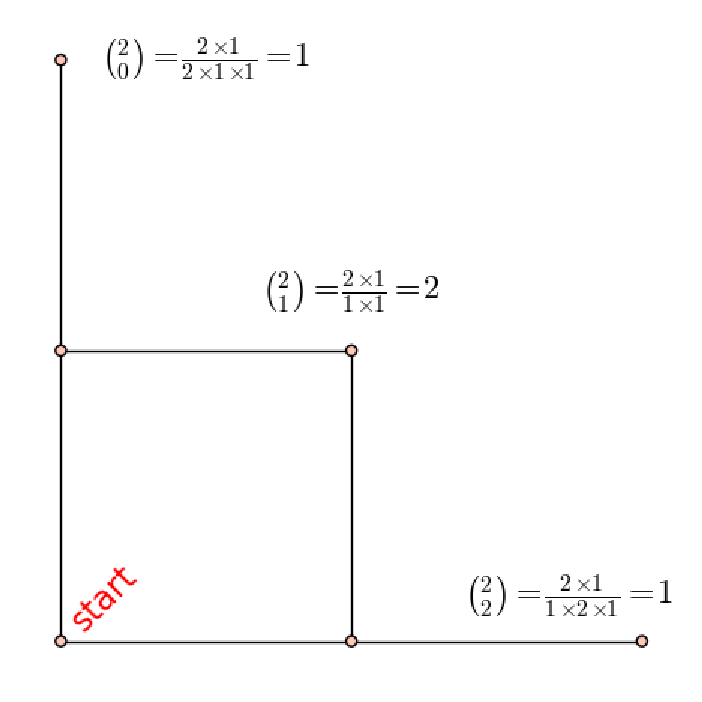
\includegraphics[width=7cm]{figures/TwoBlocksNorthEast.eps}}
\subfigure[{\scriptsize Walking three blocks north-easterly.}]{
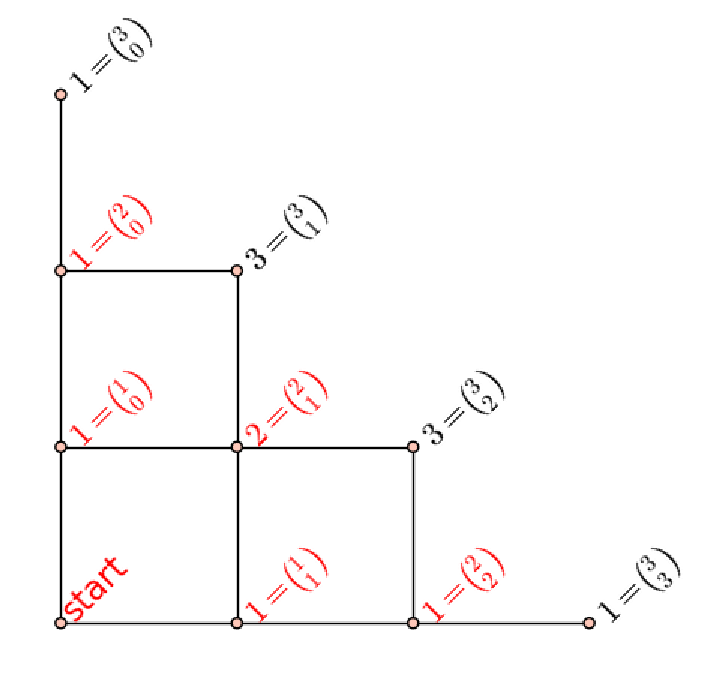
\includegraphics[width=7cm]{figures/ThreeBlocksNorthEast.eps}}
\end{figure}


\begin{Exercise}[title={Choosing Volunteers},label={xChoose3of50}]
Suppose we need three students to be the class representatives in this course.
Assume that everyone wants to be selected to keep it simple.
In how many ways can we choose these three people from the class of 50 students?
%\ExePart
%\Question
%\subQuestion Show that...
%\subQuestion In this question...
%\subsubQuestion Show that...
%\subsubQuestion Conclude...
%\subQuestion Conclude.
%\Question Show that if $b > 1$...
%\ExePart
%\Question What happens to if $b=1$?
\end{Exercise}
\begin{Answer}
We start by assuming that order does matter, that is, we have a
permutation, so that the number of ways we can select the three class
representatives is
\[^{50}P_3\;=\; \frac{50!}{(50-3)!}\;=\; \frac{50!}{47!}\]
But, because order doesn't matter,  all we have to do is to adjust our
permutation formula by a factor representing the number of  ways the objects could be in
order. Here,  three students can  be placed in order $3!$ ways, so
the required number of  ways of choosing the class representatives is:
\[ \frac{50!}{47!\, 3!}\;=\;
\frac{50\,.\, 49\,.\,48}{3\,.\,2\,.\,1}\;=\; 19,600\]
\end{Answer}

\medskip
Now, we give more formal definitions and notations that will help us make precise arguments faster when we study sampling schemes in Inference Theory.

\begin{definition}[Permutations and Factorials]
A {\bf permutation} of $n$ objects is an arrangement of $n$ distinct objects in a row.  For example, there are $2$ permutations of the two objects $\{1,2\}$:
\[
12, \qquad 21 \ ,
\]
and $6$ permutations of the three objects $\{a,b,c\}$:
\[
abc, \quad acb, \quad bac, \quad bca, \quad cab, \quad cba \ .
\]
Let the number of ways to choose $k$ objects out of $n$ and to arrange them in a row be denoted by $p_{n,k}$.  For example, we can choose two ($k=2$) objects out of three ($n=3$) objects, $\{a,b,c\}$, and arrange them in a row in six ways ($p_{3,2}$):
\[
ab, \quad ac, \quad ba, \quad bc, \quad ca, \quad cb \ .
\]
Given $n$ objects, there are $n$ ways to choose the left-most object, and once this choice has been made there are $n-1$ ways to select a different object to place next to the left-most one.  Thus, there are $n(n-1)$ possible choices for the first two positions.  Similarly, when $n>2$, there are $n-2$ choices for the third object that is distinct from the first two.  Thus, there are $n(n-1)(n-2)$ possible ways to choose three distinct objects from a set of $n$ objects and arrange them in a row.  In general,
\[
p_{n,k} = n(n-1)(n-2)\ldots (n-k+1)
\]
and the total number of permutations called `$n$ {\bf factorial}' and denoted by $n!$ is
\[
n! := p_{n,n} = n (n-1) (n-2)\ldots (n-n+1) = n (n-1) (n-2)\ldots (3) \ (2) \ (1) =: \prod_{i=1}^n i \ .
\]
\end{definition}

Some factorials to bear in mind
\[
0! := 1 \quad 1!=1, \quad 2!=2, \quad 3!=6, \quad 4!=24, \quad 5!=120 \quad 10!=3,628,800 \ .
\]
When $n$ is large we can get a good idea of $n!$ without laboriously carrying out the $n-1$ multiplications via Stirling's approximation ({\it Methodus Differentialis (1730), p.~137}) :
\[
n! \approxeq \sqrt{2 \pi n} \left( \frac{n}{e} \right)^n \ .
\]

\begin{definition}[Combinations]
The combinations of $n$ objects taken $k$ at a time are the possible choices of $k$ different elements from a collection of $n$ objects, disregarding order.  They are called the $k$-combinations of the collection.  The combinations of the three objects $\{a,b,c\}$ taken two at a time, called the $2$-combinations of $\{a,b,c\}$, are
\[
ab, \quad ac, \quad bc \ ,
\]
and the combinations of the five objects $\{1,2,3,4,5\}$ taken three at a time, called the $3$-combinations of $\{1,2,3,4,5\}$ are
\[
123, \quad 124, \quad 125, \quad 134, \quad 135, \quad 145, \quad 234, \quad 235, \quad 245, \quad 345 \ .
\]
The total number of $k$-combination of $n$ objects, called a {\bf binomial coefficient}, denoted $\binom{n}{k}$ and read ``$n$ choose $k$,'' can be obtained from $p_{n,k} = n(n-1)(n-2)\ldots(n-k+1)$ and $k! := p_{k,k}$.  Recall that $p_{n,k}$ is the number of ways to choose the first $k$ objects from the set of $n$ objects and arrange them in a row with regard to order.  Since we want to disregard order and each $k$-combination appears exactly $p_{k,k}$ or $k!$ times among the $p_{n,k}$ many permutations, we perform a division:
\[
\binom{n}{k} := \frac{p_{n,k}}{p_{k,k}} = \frac{n(n-1)(n-2)\ldots(n-k+1)}{k(k-1)(k-2)\ldots 2 \ 1} \ .
\]
\end{definition}
Binomial coefficients are often called ``Pascal's Triangle''  and attributed to Blaise Pascal's  {\it Trait\'e du Triangle Arithm\'etique} from 1653, but they have many ``fathers''.  There are earlier treatises of the binomial coefficients including Szu-y\"uan Y\"u-chien (``The Precious Mirror of the Four Elements'') by the Chinese mathematician Chu Shih-Chieh in 1303, and in an ancient Hindu classic, {\it Pi\.ngala's Chanda\d{h}\'s\=astra}, due to Hal\=ayudha (10-th century AD).



\section{Array, Sequence, Limit, \ldots}\label{S:ArraysSequencesLimitEtc}

In this section we will study a basic data structure in \Matlab called an {\bf array} of numbers.  Arrays are finite sequences and they can be processed easily in \Matlab.  The notion of infinite sequences lead to {\bf limits}, one of  the most fundamental concepts in mathematics.

For any natural number $n$, we write
$$\boxed{\langle x_{1:n} \rangle := x_1,x_{2},\ldots,x_{n-1},x_n}$$
to represent the {\bf finite sequence} of real numbers $x_1,x_2,\ldots ,x_{n-1},x_n$.
For two integers $m$ and $n$ such that $m \leq n$, we write
$$\boxed{\langle x_{m:n} \rangle := x_m,x_{m+1},\ldots,x_{n-1},x_n}$$
to represent the {\bf finite sequence} of real numbers $x_m,x_{m+1},\ldots ,x_{n-1},x_n$.  In mathematical analysis, finite sequences and their countably infinite counterparts play a fundamental role in limiting processes.  Given an integer $m$, we denote an {\bf infinite sequence} or simply a sequence as:
\[
\boxed{
\langle x_{m:\infty} \rangle := x_m, x_{m+1}, x_{m+2}, x_{m+3}, \ldots \ . }
\]
Given index set $\mathcal{I}$ which may be finite or infinite in size, a sequence can either be seen as a set of ordered pairs:
\[
\{ (i,x_i) : i \in \mathcal{I} \} \enspace ,
\]
or as a function that maps the index set to the set of real numbers:
\[
x(i)= x_i : \mathcal{I} \to \{x_{i} : i \in \mathcal{I} \} \ ,
\]
The finite sequence $\langle x_{m:n} \rangle$ has $\mathcal{I}= \{ m,m+1,m+2,m+3,\ldots,n \}$ as its index set  while an infinite sequence $\langle x_{m:\infty} \rangle$ has $\mathcal{I}= \{ m,m+1,m+2,m+3,\ldots \}$ as its index set.  A {\bf sub-sequence} $\langle x_{j:k} \rangle$ of a finite sequence $\langle x_{m:n} \rangle$ or an infinite sequence $\langle x_{m:\infty} \rangle$ is:
\[
\langle x_{j:k} \rangle = x_j,x_{j+1},\ldots,x_{k-1},x_{k} \quad \text{where, } \quad m \leq j \leq k \leq n < \infty \enspace .
\]

A rectangular arrangement of $m \cdot n$ real numbers in $m$ rows and $n$ columns is called an $m \times n$ {\bf matrix}.  The `$m \times n$' represents the {\bf size} of the matrix.  We use bold upper-case letters to denote matrices, for e.g:
$$
\X = \begin{bmatrix}
x_{1,1} & x_{1,2} & \ldots & x_{1,n-1} & x_{1,n} \\
x_{2,1} & x_{2,2} & \ldots & x_{2,n-1} & x_{2,n} \\
\vdots & \vdots & \ddots & \vdots & \vdots \\
x_{m-1,1} & x_{m-1,2} & \ldots & x_{m-1,n-1} & x_{m-1,n} \\
x_{m,1} & x_{m,2} & \ldots & x_{m,n-1} & x_{m,n}
\end{bmatrix}
$$
Matrices with only one row or only one column are called {\bf vectors}.  An $1 \times n$ matrix is called a {\bf row vector} since there is only one row and an $m \times 1$ matrix is called a {\bf column vector} since there is only one column.  We use bold-face lowercase letters to denote row and column vectors.
$$
\text{A row vector } \x = \begin{bmatrix}
x_{1} & x_{2} & \ldots & x_{n}
\end{bmatrix} = (x_1,x_2,\ldots,x_n)
$$
$$
\text{ and a column vector } \y =
\begin{bmatrix}
y_{1} \\
y_{2}  \\
\vdots \\
y_{m-1} \\
y_{m}
\end{bmatrix}
= \begin{bmatrix}
y_{1} & y_{2} & \ldots & y_{m}
\end{bmatrix}'
= (y_1,y_2,\ldots,y_m)' \ .
$$
The superscripting by $'$ is the transpose operation and simply means that the rows and columns are exchanged.  Thus the transpose of the matrix $\X$ is:
$$
\X' = \begin{bmatrix}
x_{1,1} & x_{2,1} & \ldots & x_{m-1,1} & x_{m,1} \\
x_{1,2} & x_{2,2} & \ldots & x_{m-1,2} & x_{m,2} \\
\vdots & \vdots & \ddots & \vdots & \vdots \\
x_{1,n-1} & x_{2,n-1} & \ldots & x_{m-1,n-1} & x_{m,n-1} \\
x_{1,n} & x_{2,n} & \ldots & x_{m-1,n} & x_{m,n}
\end{bmatrix}
$$
In linear algebra and calculus, it is natural to think of vectors and matrices as points (ordered $m$-tuples) and ordered collection of points in Cartesian co-ordinates.  We assume that the reader has heard of operations with matrices and vectors such as matrix multiplication, determinants, transposes, etc.  Such concepts will be introduced as they are needed in the sequel.

Finite sequences, vectors and matrices can be represented in a computer by an elementary data structure called an {\bf array}.

\begin{labwork}[Sequences as arrays]\label{LW:Seqs}
Let us learn to represent, visualise and operate finite sequences as \Matlab arrays.  Try out the commands and read the comments for clarification.
\begin{VrbM}
>> a = [17]			% Declare the sequence of one element 17 in array a
a =    17
>> % Declare the sequence of 10 numbers in array b
>> b=[-1.4508 0.6636 -1.4768 -1.2455 -0.8235 1.1254 -0.4093 0.1199 0.2043 -0.8236]
b =
   -1.4508    0.6636   -1.4768   -1.2455   -0.8235    1.1254   -0.4093    0.1199    0.2043   -0.8236
>> c = [1 2 3] 		% Declare the sequence of 3 consecutive numbers 1,2,3
c =     1     2     3
>> % linspace(x1, x2, n) generates n points linearly spaced between x1 and x2
>> r = linspace(1, 3, 3)		% Declare sequence r = c using linspace
r =     1     2     3
>> s1 = 1:10 % declare an array s1 starting at 1, ending by 10, in increments of 1
s =     1     2     3     4     5     6     7     8     9    10
>> s2 = 1:2:10  % declare an array s2 starting at 1, ending by 10, in increments of 2
s =     1     3     5     7     9
>> s2(3) % obtain the third element of the finite sequence s2
ans =     5
>> s2(2:4) % obtain the subsequence from second to fourth elements of the finite sequence s2
ans =     3     5     7
\end{VrbM}
We may visualise (as per~\hyperref[F:StemPlotDemo1]{Figure~\ref*{F:StemPlotDemo1}}) the finite sequences $\langle b_{1:n} \rangle$ stored in the array {\tt b} as the set of ordered pairs $\{(1,b_1),(2,b_2),\ldots,(10,b_{n})\}$ representing the function $b(i)=b_i:\{1,2,\ldots,n\} \to \{b_1,b_2,\ldots,b_{n} \}$ via {\bf point plot} and {\bf stem plot}  using {\tt Matlab}'s {\tt plot} and {\tt stem} commands, respectively.

\begin{figure}[hbt]
\caption{Point plot and stem plot of the finite sequence $\langle b_{1:10} \rangle$ declared as an array.\label{F:StemPlotDemo1}}
\centering   \makebox{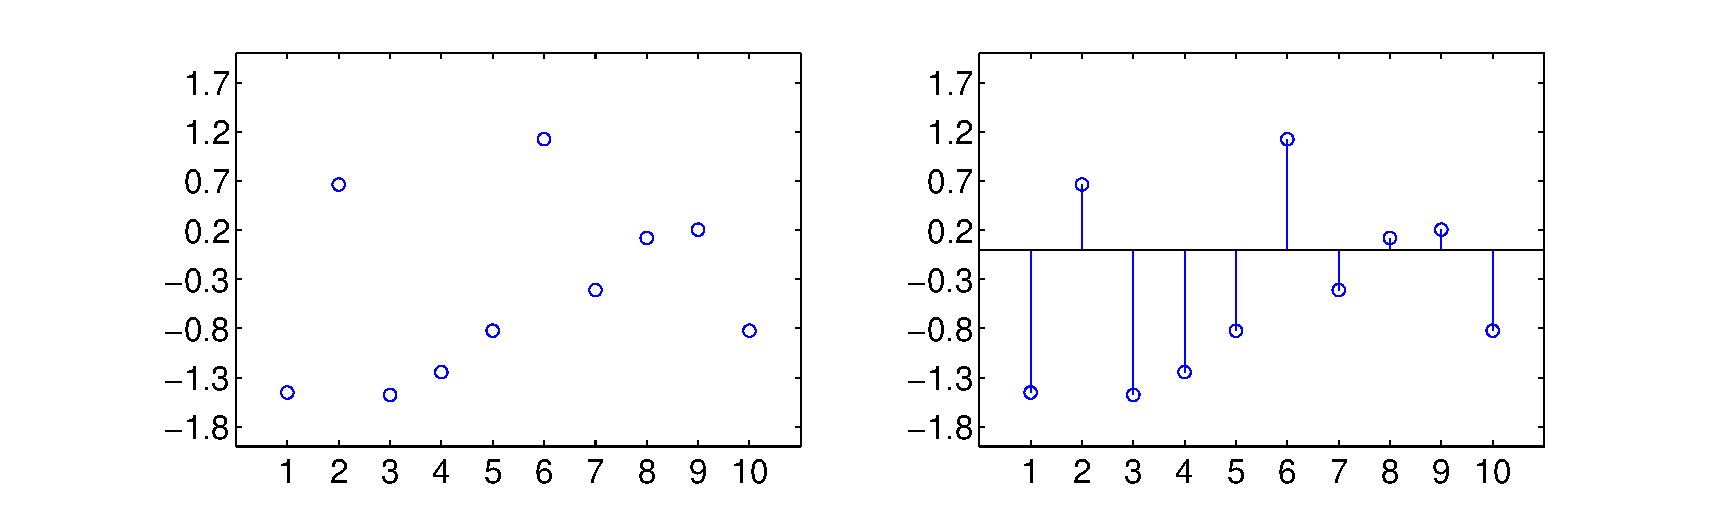
\includegraphics[width=7.0in]{figures/StemPlotDemo1}}
\end{figure}
\begin{VrbM}
>> display(b) % display the array b in memory
b =
   -1.4508    0.6636   -1.4768   -1.2455   -0.8235    1.1254   -0.4093    0.1199    0.2043   -0.8236
>> plot(b,'o') % point plot of ordered pairs (1,b(1)), (2,b(2)), ..., (10,b(10))
>> stem(b) % stem plot of ordered pairs (1,b(1)), (2,b(2)), ..., (10,b(10))
>> plot(b,'-o') % point plot of ordered pairs (1,b(1)), (2,b(2)), ..., (10,b(10)) connected by lines
\end{VrbM}
\end{labwork}

\begin{labwork}[Vectors and matrices as arrays]\label{LW:VecsMats}
Let us learn to represent, visualise and operate vectors as \Matlab arrays.  Syntactically, a vector is stored in an array exactly in the same way we stored a finite sequence.  However, mathematically, we think of a vector as an ordered $m$-tuple that can be visualised as a point in Cartesian co-ordinates.  Try out the commands and read the comments for clarification.
\begin{VrbM}
>> a = [1 2]	% an 1 X 2 row vector
>> z = [1 2 3] 	% Declare an 1 X 3 row vector z with three numbers
z =     1     2     3
>> % linspace(x1, x2, n) generates n points linearly spaced between x1 and x2
>> r = linspace(1, 3, 3)		% Declare an 1 X 3 row vector r = z using linspace
r =     1     2     3
>> c = [1; 2; 3]  	% Declare a 3 X 1 column vector c with three numbers.  Semicolons delineate columns
c =
     1
     2
     3
>> rT = r'	% The column vector (1,2,3)' by taking the transpose of r via r'
rT =
     1
     2
     3
>> y = [1 1 1] 			% y is a sequence or row vector of 3 1's
y =     1     1     1
>> ones(1,10)	% ones(m,n) is an m X n matrix of ones.  Useful when m or n is large.
ans =     1     1     1     1     1     1     1     1     1     1
\end{VrbM}
We can use two dimensional arrays to represent matrices.  Some useful built-in commands to generate standard matrices are:
\begin{VrbM}
>> Z=zeros(2,10) % the 2 X 10 matrix of zeros
Z =
     0     0     0     0     0     0     0     0     0     0
     0     0     0     0     0     0     0     0     0     0
>> O=ones(4,5) % the 4 X 5 matrix of ones
O =
     1     1     1     1     1
     1     1     1     1     1
     1     1     1     1     1
     1     1     1     1     1
>> E=eye(4) % the 4 X 4 identity matrix
E =
     1     0     0     0
     0     1     0     0
     0     0     1     0
     0     0     0     1
\end{VrbM}
We can also perform operations with arrays representing vectors, finite sequences, or matrices.
\begin{VrbM}
>> y % the array y is
y =     1     1     1
>> z % the array z is
z =     1     2     3
>> x = y + z   			% x is the sum of vectors y and z (with same size 1 X 3)
x =     2     3     4
>> y = y * 2    			% y is updated to 2 * y (each term of y is multiplied by 2)
y =     2     2     2
>> p = z .* y   			% p is the vector obtained by term-by-term product of z and y
p =     2     4     6
>> d = z ./ y    			% d is the vector obtained by term-by-term division of z and y
d =    0.5000    1.0000    1.5000
>> t=linspace(-10,10,4)		% t has 4 numbers equally-spaced between -10 and 10
t =  -10.0000   -3.3333    3.3333   10.0000
>> s = sin(t) 			% s is a vector obtained from the term-wise sin of the vector t
s =    0.5440    0.1906   -0.1906   -0.5440
>> sSq = sin(t) .^ 2	 % sSq is an array obtained from term-wise squaring ( .^ 2) of the sin(t) array
sSq =    0.2960    0.0363    0.0363    0.2960
>> cSq = cos(t) .^ 2 % cSq is an array obtained from term-wise squaring ( .^ 2) of the cos(t) array
cSq =    0.7040    0.9637    0.9637    0.7040
>> sSq + cSq % we can add the two arrays sSq and cSq to get the array of 1's
ans =     1     1     1     1
>> n = sin(t) .^2 + cos(t) .^2 	% we can directly do term-wise operation sin^2(t) + cos^2(t) of t as well
n =     1     1     1     1
>> t2 = (-10:6.666665:10)	% t2 is similar to t above but with ':' syntax of (start:increment:stop)
t2 =  -10.0000   -3.3333    3.3333   10.0000
\end{VrbM}

Similarly, operations can be performed with matrices.
\begin{VrbM}
>>  (O+O) .^ (1/2) % term-by-term square root of the matrix obtained by adding O=ones(4,5) to itself
ans =
    1.4142    1.4142    1.4142    1.4142    1.4142
    1.4142    1.4142    1.4142    1.4142    1.4142
    1.4142    1.4142    1.4142    1.4142    1.4142
    1.4142    1.4142    1.4142    1.4142    1.4142
\end{VrbM}
We can access specific rows or columns of a matrix as follows:
\begin{VrbM}
>> % declare a 3 X 3 array A of row vectors
>> A = [0.2760    0.4984    0.7513; 0.6797    0.9597    0.2551; 0.1626    0.5853    0.6991]
A =
    0.2760    0.4984    0.7513
    0.6797    0.9597    0.2551
    0.1626    0.5853    0.6991
>> A(2,:) % access the second row of A
ans =
    0.6797    0.9597    0.2551
>> B = A(2:3,:) % store the second and third rows of A in matrix B
B =
    0.6797    0.9597    0.2551
    0.1626    0.5853    0.6991
>> C = A(:,[1 3]) % store the first and third columns of A in matrix C
C =
    0.2760    0.7513
    0.6797    0.2551
    0.1626    0.6991\end{VrbM}
\end{labwork}

\begin{labwork}[Plotting a function as points of ordered pairs in two arrays]\label{LW:2Dplot}
Next we plot the function $sin(x)$ from several ordered pairs $(x_i,sin(x_i))$.  Here $x_i$'s are from the domain $[-2 \pi, 2 \pi]$.  We use the {\tt plot} function in \Matlab.  Create an M-file called {\tt MySineWave.m} and copy the following commands in it.  By entering {\tt MySineWave} in the command window you should be able to run the script and see the figure in the figure window.

\VrbMf[label=SineWave.m]{scripts/SineWave.m}

The plot was saved as an encapsulated postscript file from the File menu of the Figure window and is displayed below.
\begin{figure}[ht]
\vspace{2cm}
%FIX\centering   \makebox{\includegraphics[width=6.5in]{figures/sinewave}}
\caption{A plot of the sine wave over $[-2 \pi, 2 \pi]$.\label{F:sinfunction}}
\end{figure}
\end{labwork}

%\begin{classwork}
%Recall the trigonometric function $\sin$ with domain $\Rz$ and range $[-1,1]$.  We can explicitly refer to this function by writing:
%\[
%\sin : \Rz \to [-1,1]
%\]
%\begin{figure}[htpb]
%\caption{A depiction of the function $\sin$ and the inverse image $\sin^{[-1]}(0) =\{i \pi : i \in \Zz\}$.\label{F:sinfunction}}
%\vspace{5cm}
%\end{figure}
%\end{classwork}

%Continuity

\section{Elementary Real Analysis}



\subsection{Limits of Real Numbers -- A Review}\label{S:AnalysisRefresher}

%TODO
%Differentiability

%Riemann Integral


Let us first recall some elementary ideas from real analysis.
\begin{definition}[Convergent sequence of real numbers]\label{Dfn:ConvReals}
A sequence of real numbers  $\langle x_i \rangle_{i=1}^{\infty} := x_1,x_2,\ldots$ is said to converge to a limit $a \in \Rz$ and denoted by:
\[
\lim_{i \to \infty} x_i = a \ ,
\]
if for every natural number $m \in \Nz$, a natural number $N_m \in \Nz$ exists such that for every $j \geq N_m$, $|x_j-a| \leq \frac{1}{m}$.
\end{definition}

In words, $\lim_{i \to \infty} x_i = a$ means the following: no matter how small you make $\frac{1}{m}$ by picking as large an $m$ as you wish, I can find an $N_m$, that may depend on $m$, such that every number in the sequence beyond the $N_m$-th element is within distance $\frac{1}{m}$ of the limit $a$.

\begin{example}[Limit of a sequence of $17$s]\label{EX:limOf17s}
Let $\langle x_i \rangle_{i=1}^{\infty} = 17, 17, 17, \ldots$. Then $\lim_{i \to \infty} x_i = 17$.  This is because for every  $m \in \Nz$, we can take $N_m=1$ and satisfy the definition of the limit, i.e.:
\[
\text{for every }  j \geq N_m= 1, \  |x_j-17|=|17-17|=0\leq \frac{1}{m} \ .
\]
\end{example}

\begin{example}[Limit of $1/i$]\label{EX:limin1overi}
Let $\langle x_i \rangle_{i=1}^{\infty} = \frac{1}{1},\frac{1}{2},\frac{1}{3}, \ldots$, i.e.~$x_i = \frac{1}{i}$, then $\lim_{i \to \infty} x_i = 0$.  This is because for every  $m \in \Nz$, we can take $N_m=m$ and satisfy the definition of the limit, i.e.:
\[
\text{for every }  j \geq N_m= m, \  |x_j-0|=\left| \frac{1}{j}-0 \right|=\frac{1}{j} \leq \frac{1}{m} \ .
\]
\end{example}
However, several other sequences also approach the limit $0$.  Some such sequences that approach the limit $0$ from the right are:
\begin{flalign*}
\langle x_{1:\infty} \rangle =  \frac{1}{1},\frac{1}{4},\frac{1}{9}, \ldots \qquad \text{and} \qquad  \langle x_{1:\infty} \rangle  =  \frac{1}{1},\frac{1}{8},\frac{1}{27},\ldots \enspace ,
\end{flalign*}
and some that approach the limit $0$ from the left are:
\begin{flalign*}
\langle x_{1:\infty} \rangle =  -\frac{1}{1},-\frac{1}{2},-\frac{1}{3}, \ldots \qquad \text{and} \qquad
\langle x_{1:\infty} \rangle =  -\frac{1}{1},-\frac{1}{4},-\frac{1}{9}, \ldots \enspace ,
\end{flalign*}
and finally some that approach $0$ from either side are:
\begin{flalign*}
\langle x_{1:\infty} \rangle =  -\frac{1}{1},+\frac{1}{2},-\frac{1}{3}, \ldots \qquad \text{and} \qquad
\langle x_{1:\infty} \rangle = -\frac{1}{1},+\frac{1}{4},-\frac{1}{9} \ldots \enspace .
\end{flalign*}
When we do not particularly care about the specifics of a sequence of real numbers $\langle x_{1:\infty} \rangle$, in terms of the exact values it takes for each $i$, but we are only interested that it converges to a limit $a$ we write:
\[
x \to a
\]
and say that $x$ approaches $a$.  If we are only interested in those sequences that converge to the limit $a$ from the right or left, we write:
\[
x \to a^+ \qquad \text{or} \qquad x \to a^-
\]
and say $x$ approaches $a$ from the right or left, respectively.

\begin{definition}[Limits of Functions]\label{D:LimitofRealFunction}
We say a function $f(x):\Rz \to \Rz$ has a {\bf limit} $L \in \Rz$ as $x$ approaches $a$ and write:
\[
\lim_{x \to a} f(x)=L \ ,
\]
provided $f(x)$ is arbitrarily close to $L$ for all values of $x$ that are sufficiently close to, but not equal to, $a$.  We say that $f$ has a {\bf right limit} $L_R$ or {\bf left limit} $L_L$ as $x$ approaches $a$ from the left or right, and write:
\[
\lim_{x \to a^+} f(x)=L_R  \qquad \text{ or } \qquad \lim_{x \to a^-} f(x)=L_L \ ,
\]
provided $f(x)$ is arbitrarily close to $L_R$ or $L_L$ for all values of $x$ that are sufficiently close to, but not equal to, $a$ from the right of $a$ or the left of $a$, respectively.  When the limit is not an element of $\Rz$ or when the left and right limits are distinct, we say that the limit does not exist.
\end{definition}

\begin{example}[Limit of $1/x^2$]
Consider the function $f(x)=\frac{1}{x^2}$.  Then
\[
\lim_{x \to 1} f(x) = \lim_{x \to 1} \frac{1}{x^2} = 1
\]
exists since the limit $1 \in \Rz$, and the right and left limits are the same:
\[
\lim_{x \to 1^+} f(x) = \lim_{x \to 1^+} \frac{1}{x^2} = 1 \qquad \text{and} \qquad
\lim_{x \to 1^-} f(x) = \lim_{x \to 1^-} \frac{1}{x^2} = 1 \ .
\]
However, the following limit does not exist:
\[
\lim_{x \to 0} f(x) = \lim_{x \to 0} \frac{1}{x^2} = \infty
\]
since $\infty \notin \Rz$.
\end{example}

Let us next look at some limits of functions that exist despite the function itself being undefined at the limit point.

\begin{example}[Limit of $(1+x)^{\frac{1}{x}}$]\label{EX:LimitToE}
The limit of $f(x)=(1+x)^{\frac{1}{x}}$ as $x$ approaches $0$ exists and it is the Euler's constant $e$ :
\begin{eqnarray*}
\lim_{x \to 0} f(x)
&=& \lim_{x \to 0} (1+x)^{\frac{1}{x}}\\
&=& \lim_{x \to 0} (x+1)^{(1/x)} \quad \text{Indeterminate form of type $1^\infty$.}\\
&=& \exp\left(\lim_{x\to 0} \log((x+1)^{(1/x)})\right) \quad \text{Transformed using $\exp(\lim_{x\to 0} \log((x+1)^{(1/x)}))$} \\
&=& \exp\left(\lim_{x\to 0} (\log(x+1))/x\right) \quad \text{Indeterminate form of type $0/0$.}\\
&=& \exp\left( \lim_{x\to 0} \frac{ d\log(x+1)/ dx}{ dx/ dx} \right) \quad \text{Applying L'Hospital's rule} \\
&=&  \exp\left(\lim_{x\to 0} 1/(x+1)\right) \quad \text{limit of a quotient is the quotient of the limits}\\
&=&  \exp\left(1/(\lim_{x \to 0} (x+1))\right) \quad \text{The limit of $x+1$ as $x$ approaches $0$ is $1$}\\
&=& \exp(1)=e \approxeq 2.71828 \enspace .
\end{eqnarray*}
\[
\lim_{x \to 0} f(x) = \lim_{x \to 0} (1+x)^{\frac{1}{x}} = e \approxeq 2.71828 \ .
\]
Notice that the above limit exists despite the fact that $f(0) = (1+0)^{\frac{1}{0}}$ itself is undefined and does not exist.
\end{example}

\begin{example}[Limit of $\frac{x^3-1}{x-1}$]
For $f(x)=\frac{x^3-1}{x-1}$, this limit exists:
\[
\lim_{x \to 1} f(x) = \lim_{x \to 1} \frac{x^3-1}{x-1}
=  \lim_{x \to 1} \frac{(x-1)(x^2+x+1)}{(x-1)}
= \lim_{x \to 1} x^2+x+1 = 3 \,
\]
despite the fact that $f(1)=\frac{1^3-1}{1-1}=\frac{0}{0}$ itself is undefined and does not exist.
\end{example}

Next we look at some examples of limits at infinity.
\begin{example}[Limit of $(1-\frac{\lambda}{n})^n$]\label{EX:LimitExpofLambda}
The limit of $f(n)=\left( 1-\frac{\lambda}{n} \right)^n$ as $n$ approaches $\infty$ exists and it is $e^{-\lambda}$ :
\[
\lim_{n \to \infty} f(n) = \lim_{n \to \infty} \left( 1-\frac{\lambda}{n} \right)^n = e^{-\lambda} \ .
\]
\end{example}

\begin{example}[Limit of $(1-\frac{\lambda}{n})^{-\alpha}$]\label{EX:Limit1MinusLambdaOverNToMinusK}
The limit of $f(n)=\left( 1-\frac{\lambda}{n} \right)^{-\alpha}$, for some $\alpha>0$, as $n$ approaches $\infty$ exists and it is $1$ :
\[
\lim_{n \to \infty} f(n) = \lim_{n \to \infty} \left( 1-\frac{\lambda}{n} \right)^{-\alpha} = 1 \ .
\]
\end{example}

\begin{definition}[Continuity of a function]
We say a real-valued function $f(x):D \to \Rz$ with the domain $D \subset \Rz$ is {\bf right continuous} or {\bf left continuous} at a point $a \in D$, provided:
\[
\lim_{x \to a^+} f(x) = f(a) \qquad \text{ or } \qquad
\lim_{x \to a^-} f(x) = f(a) \ ,
\]
respectively.  We say $f$ is {\bf continuous} at $a \in D$, provided:
\[
\lim_{x \to a^+} f(x) = f(a) =
\lim_{x \to a^-} f(x) \ .
\]
Finally, $f$ is said to be continuous if $f$ is continuous at every $a \in D$.
\end{definition}
\begin{example}[Discontinuity of $f(x)=(1+x)^{\frac{1}{x}}$ at $0$]
Let us reconsider the function $f(x)=(1+x)^{\frac{1}{x}}:\Rz \to \Rz$.  Clearly, $f(x)$ is continuous at $1$, since:
\[
\lim_{x \to 1} f(x) = \lim_{x \to 1}(1+x)^{\frac{1}{x}} = 2 = f(1)=(1+1)^{\frac{1}{1}} \ ,
\]
but it is not continuous at $0$, since:
\[
\lim_{x \to 0} f(x) = \lim_{x \to 0} (1+x)^{\frac{1}{x}} = e \approxeq 2.71828 \neq f(0) = (1+0)^{\frac{1}{0}} \ .
\]
Thus, $f(x)$ is not a continuous function over $\Rz$.
\end{example}

%Here is a summary of the notations we have learned here.
%\begin{table}[t]
%\centering
%\begin{tabular}{cc}
%$\Omega$&\\
%$\to$&\\
%$f^{[-1]}$&\\
%$lim _{i\to \infty}x_i=a$&\\
%${x_i}^\infty_{i=1}$&\\
%$a^+$ and $a^-$&\\
%$\approxeq$ & \\
%\end{tabular}
%%\caption{}
%%\label{tab:}
%\end{table}

%\begin{table}[htb]
%\centering
%{\normalsize
%\begin{tabular}{| l | l |}
%\hline
%Symbol & Meaning\\ \hline
%$\Nz$& The set of natural numbers $\{1,2,3,\ldots\}$\\
%$\Zz$&The set of integers $\{\ldots,-3,-2,-1,0,1,2,3,\ldots\}$\\
%$\Dz_+$& The set of non-negative integers $\{0,1,2,3,\ldots\}$\\
%$\Rz$& The set of real numbers\\ \hline
%\end{tabular}
%}
%\caption{Analysis Symbol Table \label{T:SymbTableAnalysis}}
%\end{table}

\section{Elementary Number Theory}\label{S:ElemNumTh}
We introduce basic notions that we need from elementary number theory here.  These notions include integer functions and modular arithmetic as they will be needed later on.

For any real number $x$:
\begin{flalign*}
\lfloor x \rfloor &:= \max\{y: y \in \Zz \text{ and } y \leq x\}, \text{i.e., the greatest integer less than or equal to $x$ (the {\bf floor} of $x$),}\\
\lceil x \rceil &:= \min\{y: y \in \Zz \text{ and } y \geq x\}, \text{i.e., the least integer greater than or equal to $x$ (the {\bf ceiling} of $x$).}
\end{flalign*}

\begin{example}[Floors and ceilings]
\[
\lfloor 1 \rfloor = 1, \quad \lceil 1 \rceil = 1, \quad \lfloor 17.8 \rfloor = 17, \quad   \lfloor -17.8 \rfloor = -18, \quad \lceil \sqrt{2} \rceil = 2, \quad \lfloor \pi \rfloor = 3, \quad \lceil \frac{1}{10^{100}} \rceil = 1.
\]
\end{example}

\begin{labwork}[Floors and ceilings in \Matlab]\label{LW:FloorCeil}  We can use \Matlab functions {\tt floor} and {\tt ceil} to compute $\lfloor x \rfloor$ and $\lceil x \rceil$, respectively.  Also, the argument  $x$ to these functions can be an array.
\begin{VrbM}
>> sqrt(2) % the square root of 2 is
ans =    1.4142
>> ceil(sqrt(2)) % ceiling of square root of 2
ans =     2
>> floor(-17.8) % floor of -17.8
ans =   -18
>> ceil([1 sqrt(2) pi -17.8 1/(10^100)]) %the ceiling of each element of an array
ans =     1     2     4   -17     1
>> floor([1 sqrt(2) pi -17.8 1/(10^100)]) % the floor of each element of an array
ans =     1     1     3   -18     0
\end{VrbM}
\end{labwork}

\begin{classwork}[Relations between floors and ceilings]
Convince yourself of the following formulae.  Use examples, plots and/or formal arguments.
\begin{flalign*}
\lceil x \rceil &= \lfloor x \rfloor \iff x \in \Zz \\
\lceil x \rceil &= \lfloor x \rfloor + 1 \iff x \notin \Zz \\
\lfloor -x \rfloor &= - \lceil x \rceil \\
x-1 < \lfloor x \rfloor \leq x & \leq \lceil x \rceil < x+1
\end{flalign*}
\end{classwork}

Let us define modular arithmetic next.  Suppose $x$ and $y$ are any real numbers, i.e.~$x,y \in \Rz$, we define the binary operation called ``$x \mod y$'' as:
\[
x \mod y :=
\begin{cases}
x - y \lfloor x/y \rfloor & \text{if $y \neq 0$} \\
x  & \text{if $y = 0$}
\end{cases}
\]
%} % end of remove


%\clearpage
\chapter{Probability Model}\label{S:ProbModel}

\section{Experiments}\label{S:Experiments}

Ideas about chance events and random behaviour arose out of thousands of
years of game playing, long before any attempt was made to use
mathematical reasoning about them. Board and dice games were well known
in Egyptian times, and Augustus Caesar gambled with dice. Calculations
of odds for gamblers were put on a proper theoretical basis by Fermat
and Pascal in the early 17th century.

\begin{definition}
An {\bf experiment} is an activity or procedure that produces distinct, well-defined possibilities called {\bf outcomes}.  
The set  of all outcomes   is called the {\bf sample space}, and is denoted by $\Omega$.

The subsets of $\Omega$ are called {\bf events}.  
A single outcome, $\omega$, when seen as a subset of $\Omega$, as in
$\{\omega\}$, is called a  {\bf simple event}.

Events, $E_1,\, E_2\, \dots \, E_n$,  that cannot occur at the same time are called {\bf mutually exclusive} events, or {\bf pair-wise disjoint} events.  This means that $E_i
\cap E_j = \emptyset $ where $i\not=j$.
\end{definition}



\begin{example}
Some standard examples of experiments are the following:

\bit

\item $\Omega=\{ {\textsf{Defective, Non-defective}} \}$ if our
  experiment is to inspect a light bulb.

There are only two outcomes here, so   $\Omega = \{ \omega_1, \omega_2\}$
where $\omega_1= {\textsf{Defective}}$ and  $\omega_2 =
{\textsf{Non-defective}}$.


\item $\Omega=\{ {\textsf{Heads, Tails}} \}$ if our experiment is to
  note the outcome of a coin toss.


This time, $\Omega=\{ \omega_1, \omega_2\}$ where $\omega_1= {\textsf{Heads}}$ and  $\omega_2 = {\textsf{Tails}}$.


\item If our experiment is to roll a die  then there are six outcomes corresponding to
  the number that shows on the top. For this experiment,
  $\Omega = \{\mathsf{1,2,3,4,5,6}\}$.


Some examples of events are the set of odd numbered outcomes
$A=\{\mathsf{1,3,5}\}$, and  the set of
even numbered outcomes $B=\{\mathsf{2,4,6}\}$.


The simple events  of $\Omega$ are $\{\sf{1}\}, \{\sf{2}\}, \{\sf{3}\}, \{\sf{4}\}, \{\sf{5}\}$, and $\{\sf{6}\}$.

\eit
\end{example}


The outcome of a random experiment is uncertain until it is performed and observed.  
Note that sample spaces need to reflect the problem in hand.  
The example below is to convince you that an experiment's sample space is merely a collection of distinct elements called outcomes and these outcomes have to be {\em discernible in some well-specified sense} to the experimenter!


\begin{example}
\label{Eg:SensoryDiscerningExperiments} 
Consider a generic
  die-tossing experiment by a human experimenter. Here \newline $\Omega=
  \{\omega_1,\omega_2,\omega_3,\ldots,\omega_6\}$, but the
  experiment might correspond to rolling a die whose faces are:
\begin{enumerate}
\item sprayed with six different scents (nose!), or
\item studded with six distinctly flavoured candies (tongue!), or
\item contoured with six distinct bumps and pits (touch!), or
\item acoustically discernible at six different frequencies (ears!), or
\item painted with six different colours (eyes!), or
\item marked with six different numbers $\mathsf{1,2,3,4,5,6}$ (eyes!), or , \ldots
\end{enumerate}
These six experiments are  equivalent as far as probability goes.
\end{example}


\begin{definition}
{A {\bf trial} is a single performance of an experiment and it
  results in an outcome.}
\end{definition}



\begin{example}
Some standard examples of a trial are:

\bit

\item A roll of a die.

\item A toss of a coin.

\item A release of a chaotic double pendulum.

\eit
\end{example}

An experimenter often performs more than one trial.  Repeated trials of an experiment forms the basis of science and engineering as the experimenter learns about the phenomenon by repeatedly performing the same mother experiment with possibly different outcomes.  This repetition of trials in fact provides the very motivation for the definition of probability.

\begin{definition}{An {\bf ${\mathbf n}$-product experiment} is obtained by
    repeatedly performing $n$ trials of some experiment. 
    %This experiment is often called the mother experiment.% Raaz substituted to avoid the ambiguous reference to 'This'
    The experiment that is repeated is called the ``mother'' experiment.}
\end{definition}



\begin{example}[Toss a coin $n$ times]\label{EX:T3X}
Suppose our experiment entails tossing a coin $n$ times and recording ${\tt H}$ for Heads and ${\tt T}$ for Tails.  When $n=3$, one possible outcome of this experiment is ${\tt HHT}$, ie.~a Head followed by another Head and then a Tail.  Seven other outcomes are possible.  
%Below, we refer to this experiment by the symbol $\E{E}_{\theta}^{3}$.  More generally, we refer to the experiment of tossing a coin $n$ times as $\E{E}_{\theta}^{n}$ and sometimes refer to $\E{E}_{\theta}^{1}$ by $\E{E}_{\theta}$ for simplicity.  The reason for the $\theta$ subscrip will become apparent as we develop the theory.
\end{example}


The sample space for ``toss a coin three times" experiment %$\E{E}_{\theta}^{3}$ %\hyperref[EX:T3X]{Experiment \ref*{EX:T3X}} of tossing a coin 3 times 
is:
\[
\Omega = \{ {\tt H}, {\tt T} \}^3 =  \{ {\tt HHH}, {\tt HHT}, {\tt HTH}, {\tt HTT}, {\tt THH}, {\tt THT}, {\tt TTH}, {\tt TTT}  \} \ ,
\]
with a particular sample point or outcome $\omega = {\tt HTH}$, and another distinct outcome $\omega' = {\tt HHH}$.  An event, say $A$, that `at least two Heads occur' is the following subset of $\Omega$:
\[
A = \{ {\tt HHH}, {\tt HHT}, {\tt HTH}, {\tt THH} \} \ .
\]
Another event, say $B$, that `no Heads occur' is:
\[
B = \{{\tt TTT}\}
\]
Note that the event $B$ is also an outcome or sample point.  Another interesting event is the empty set $\emptyset  \subset \Omega$.  The event that `nothing in the sample space occurs' is $\emptyset$.

\begin{classwork}[A thrice-bifurcating tree of outcomes]
Can you think of a graphical way to enumerate the outcomes of the Experiment~\ref{EX:T3X}%$\E{E}_{\theta}^{3}$
?  Draw a diagram of this under the caption of \hyperref[F:T3X]{Figure~\ref*{F:T3X}}, using the caption as a hint (in other words, draw your own \hyperref[F:T3X]{Figure~\ref*{F:T3X}}).
\begin{figure}[htpb]
\caption{A binary tree whose leaves are all possible outcomes.\label{F:T3X}}
\vspace{4cm}
\end{figure}
\end{classwork}

\remove{
In \hyperref[LW:T3X]{Labwork~\ref*{LW:T3X}} we implement \hyperref[AL:T3X]{Algorithm~\ref*{AL:T3X}} to  print all the outcomes.  The algorithm uses {\bf for loops} to reach the leaves (outcomes of $\E{E}_{\theta}^{3}$) of the binary tree.
\begin{algorithm}[htpb]
\caption{List $\Omega$ for ``Toss a Coin Three Times" experiment $\E{E}_{\theta}^{3}$}
\label{AL:T3X}
\begin{algorithmic}[1]
\STATE {\it input:} nothing

\STATE {\it output:} print/list all outcomes of $\E{E}_{\theta}^{3}$ 

\STATE {\it initialize:} ${\bf SampleSpace1Toss} = \{ {\tt H}, {\tt T} \}$  \COMMENT{{\tiny ${\bf SampleSpace1Toss}[1]={\tt H}$ and ${\bf SampleSpace1Toss}[2]={\tt T}$}}
\FOR{$i=1$ to $2$} 
\FOR{$j=1$ to $2$}
\FOR{$k=1$ to $2$}
\STATE {
 Print ${\bf SampleSpace1Toss}[i]$ ${\bf SampleSpace1Toss}[j]$ ${\bf SampleSpace1Toss}[k]$ \\
Print `` , "  \COMMENT{{\tiny print a comma character to delimit outcomes}}
}
\ENDFOR
\ENDFOR
\ENDFOR
\end{algorithmic}
\end{algorithm}

\begin{labwork}[Three for loops for the thrice-bifurcating tree]\label{LW:T3X}
Let's write a {\sc Matlab} code in a script file named {\tt OutcomesOf3Tosses.m} that implements \hyperref[AL:T3X]{Algorithm~\ref*{AL:T3X}} to print all the outcomes of $\E{E}_{\theta}^{3}$.  You need to go to the File menu and create a new file named {\tt OutcomesOf3Tosses.m} Run it in the command window.
\begin{VrbM}
>> type OutcomesOf3Tosses.m

SampleSpace1Toss='HT';	% declare a string vector or character array
% SampleSpace1Toss is the name of the char array
SampleSpace1Toss(1);		% access the first element 'H' this way
SampleSpace1Toss(2);		% access the second element 'T' this way
% Now let's write the routine for listing the sample space of 'toss 3 times'
w=' ';		% declare w to be the character ' '
for i = 1:1:2		% for loop for variable i = start:increment:end
  for j = 1:1:2		% for loop for variable j
    for k = 1:1:2	% for loop for variable j
     % next we concatenate using strcat -- strcat('A','B','C','D') concatenates the 4 char arrays
     x = strcat(SampleSpace1Toss(i),SampleSpace1Toss(j),SampleSpace1Toss(k),' , '); % ' ,' delimited outcome
     w = strcat(w,x); % recursively store the outcomes in a new array w
    end
  end
end
w		% print w at the end of the three for loops
>> lab1work4
>> SampleSpace1Toss(1)
ans = H
>> SampleSpace1Toss(2)
ans = T
>> w
w = HHH ,HHT ,HTH ,HTT ,THH ,THT ,TTH ,TTT ,
\end{VrbM}
\end{labwork}
}


\begin{framed}
EXPERIMENT SUMMARY\\

\begin{tabular}{rcl}
Experiment &$-$& an activity producing distinct outcomes.\\
$\Omega$ &$-$& set of all outcomes of the experiment.\\
$\omega$ &$-$& an individual outcome in $\Omega$, called a simple event.\\
$A\subseteq \Omega$ &$-$& a subset $A$ of $\Omega$ is an event.\\
Trial &$-$& one performance of an experiment resulting in 1 outcome.\\
\end{tabular}
\end{framed}


\section{Probability}\label{S:Probability}
The  mathematical model for probability or the probability model is an axiomatic system that may be motivated by the intuitive idea of `long-term relative frequency'.  If the axioms and definitions are intuitively motivated, the probability model simply follows from the application of logic to these axioms and definitions.  No attempt to define probability in the real world is made. However, the application of probability models to real-world problems through statistical experiments has a fruitful track record.  In fact, you are here for exactly this reason.

\begin{idea}[The long-term relative frequency (LTRF) idea]
Suppose we are interested in the fairness of a coin, i.e.~if landing Heads has the same ``probability" as landing Tails.  We can toss it $n$ times and call 
$N({\tt H},n)$ the fraction of times we observed Heads out of $n$ tosses.
Suppose that after conducting the tossing experiment $1000$ times, we rarely observed Heads, e.g.~$9$ out of the $1000$ tosses, then $N({\tt H},1000)=9/1000=0.009$.  Suppose we continued the number of tosses to a million and found that this number approached closer to $0.1$, or, more generally, $N({\tt H},n) \to 0.1$ as $n \to \infty$.  We might, at least intuitively, think that the coin is unfair and has a lower ``probability'' of $0.1$ of landing Heads.  We might think that it is fair had we observed $N({\tt H},n) \to 0.5$ as $n \to \infty$.  Other crucial assumptions that we have made here are:
\begin{enumerate}
\item {\bf Something Happens}: Each time we toss a coin, we are certain to observe Heads {\bf or} Tails, denoted by ${\tt H} \cup {\tt T}$.  The probability that ``something happens'' is $1$.  More formally:
\[
N({\tt H} \cup {\tt T},n)= \frac{n}{n} = 1.
\]
This is an intuitively reasonable assumption that simply says that one of the possible outcomes is certain to occur, provided the coin is not so thick that it can land on or even roll along its circumference.

\item {\bf Addition Rule}: Heads and Tails are mutually exclusive events in any given toss of a coin, i.e.~they cannot occur simultaneously.  The intersection of mutually exclusive events is the empty set and is denoted by ${\tt H} \cap {\tt T} = \emptyset$. The event ${\tt H} \cup {\tt T}$, namely that the event that ``coin lands Heads {\bf or} coin lands Tails" satisfies:
\[
N({\tt H} \cup {\tt T},n)= N({\tt H},n) + N({\tt T},n) .
\]
\item The coin-tossing experiment is repeatedly performed in an {\bf independent} manner, i.e.~the outcome of any individual coin-toss does not affect that of another.  This is an intuitively reasonable assumption since the coin has no memory and the coin is tossed identically each time.
\end{enumerate}
\end{idea}

We will use the LTRF idea more generally to motivate a mathematical model of probability called probability model.  Suppose $A$ is an event associated with some experiment $\E{E}$, so that $A$ either does or does not occur when the experiment is performed.  We want the probability that event $A$ occurs in a specific performance of $\E{E}$, denoted by $\p(A)$, to intuitively mean the following:  if one were to perform a super-experiment $\E{E}^{\infty}$ by independently repeating the experiment $\E{E}$ and recording $N(A,n)$, the fraction of times $A$ occurs in the first $n$ performances of $\E{E}$ within the super-experiment $\E{E}^{\infty}$. Then the LTRF idea suggests:
\begin{equation}\label{E:NofAn}
N(A,n) :=  \frac{\text{Number of times $A$ occurs}}{n=\text{Number of performances of $\E{E}$}} \to \p(A), \ as \quad  n \to \infty
\end{equation}

Now, we are finally ready to define probability.
\begin{definition}[Probability]\label{D:Prob}
Let $\E{E}$ be an experiment with sample space $\Omega$.  Let $\C{F}$ denote a suitable collection of events in $\Omega$ that satisfy the following conditions:
\begin{enumerate}
\item It (the collection) contains the sample space:
$\boxed{
\Omega \in \C{F} }$.
\item It is closed under complementation:
$\boxed{
A \in \C{F} \quad \implies \quad A^c \in \C{F} }$.
\item It is closed under countable unions:
$\boxed{
A_1, A_2, \ldots \in \C{F} \quad \implies \quad \bigcup_{i} {A_i} := A_1 \cup A_2 \cup \cdots \in \C{F} }$.
\end{enumerate}
Formally, this collection of events is called a {\bf sigma field} or a {\bf sigma algebra}.  Our experiment $\E{E}$ has a sample space $\Omega$ and a collection of events $\C{F}$ that satisfy the three condition. 

Given a double, e.g. $(\Omega, \C{F})$, {\bf probability} is just a function $\p$ which assigns each event $A \in \C{F}$ a number $\p(A)$ in the real interval $[0,1]$, i.e.~$\boxed{\p : \C{F} \to [0,1] }$, such that:
\begin{enumerate}
\item The `Something Happens' axiom holds, i.e.~$\boxed{\p(\Omega) = 1}$. 
\item The `Addition Rule' axiom holds, i.e.~for events $A$ and $B$:
$$
\boxed{
A \cap B = \emptyset \quad \implies \quad \p(A \cup B) = \p(A) + \p(B)
} \ .
$$
\end{enumerate}
\end{definition}
\subsection{Consequences of our Definition of Probability}\label{S:ConseqDefProb}
It is important to realize that we accept the `addition rule' as an axiom in our mathematical definition of probability (or our probability model) and we do {\bf not} prove this rule.  However, the facts which are stated ({\scriptsize with proofs}) below, are logical consequences of our definition of probability:
\begin{enumerate}
\item For any event $A$, $\boxed{\p(A^c) = 1 - \p(A)}$.
{\scriptsize
\begin{proof}
One line proof.
\[
\overbrace{\p(A) + \p(A^c)}^{LHS} \underbrace{=}_{+~\text{rule}~\because A \cap A^c = \emptyset} \p(A \cup A^c) \underbrace{=}_{A \cup A^c = \Omega} \p(\Omega) \underbrace{=}_{\because~\p(\Omega) = 1} \overbrace{1}^{RHS} \quad \underbrace{\Longrightarrow}_{LHS-\p(A)~\&~RHS-\p(A)} \quad \p(A^c) = 1-\p(A)
\]
\end{proof}
}
\begin{itemize}
\item If $A = \Omega$ then $A^c = \Omega^c = \emptyset$ and 
$\boxed{\p(\emptyset) = 1-\p(\Omega) = 1-1 = 0}$.
\end{itemize}

\item For any two events $A$ and $B$, we have the {\bf inclusion-exclusion principle}:
\[
\boxed{
\p(A \cup B) = \p(A) + \p(B) - \p(A \cap B)
}.
\]
{\scriptsize
\begin{proof}
Since: 
\begin{eqnarray}
\quad A = (A \setminus B) \cup (A \cap B) & \quad \text{and} \quad & (A \setminus B) \cap (A \cap B) = \emptyset, \notag \\
\quad A \cup B = (A \setminus B) \cup B & \quad \text{and} \quad & (A \setminus B) \cap B = \emptyset \notag
\end{eqnarray}
the addition rule implies that:
\begin{eqnarray}
\p(A) &=& \p(A \setminus B) + \p(A \cap B) \notag \\
\p(A \cup B) &=& \p(A \setminus B) + \p(B) \notag
\end{eqnarray}
Substituting the first equality above into the second, we get:
\[
\p(A \cup B) = \p(A \setminus B) + \p(B) = \p(A) - \p(A \cap B) + \p(B)
\]
\end{proof}
}
\item From inclusion-exclusion principle we get {\bf Boole's inequality}: for any two events $A, B$
\[
\p(A \cup B) \leq \p(A) + \p(B)
\]
\item The inclusion-exclusion principle extends similarly to any three events $A_1,A_2,A_3$ as follows:
\[
\p(A_1 \cup A_2 \cup A_3) = \p(A_1) + \p(A_2) + \p(A_3) - \p(A_1 \cap A_2) - \p(A_1 \cap A_3) - \p(A_2 \cap A_3) + \p(A_1 \cap A_2 \cap A_3)
\]
and generalises to any $n$ events $A_1,A_2,\ldots,A_n$ as folows:
\[
\p \left( \bigcup_{i=1}^n A_i \right) = \sum_{i=1}^n \p(A_i) - \sum_{i<j} \p(A_i \cap A_j) + \sum_{i<j<k} \p(A_i \cap A_j \cap A_k) + \cdots + (-1)^{n-1} \sum_{i< \cdots <n} \p \left( \bigcap_{i=1}^n A_i \right)
\]

{\scriptsize
\begin{proof} See the counting argument in \url{https://en.wikipedia.org/wiki/Inclusion\%E2\%80\%93exclusion_principle} if you are curious.
\end{proof}
}  
\item Once again by the inclusion-exclusion principle, the Boole's inequality generalises to any $n$ events $A_1,A_2,\ldots,A_n$ as folows:
\[
\p \left( \bigcup_{i=1}^n A_i \right) \leq \sum_{i=1}^n \p(A_i)
\]
\item For a sequence of mutually disjoint events $A_1, A_2, A_3, \ldots, A_n$: 
\[
\boxed{
A_i \cap A_j = \emptyset \quad \text{for any $i \neq j$} \quad \implies \quad \p(A_1 \cup A_2 \cup \cdots \cup A_n) = \p(A_1)+\p(A_2)+ \cdots + \p(A_n)} .
\]
{\scriptsize
\begin{proof}
If $A_1, A_2, A_3$ are mutually disjoint events, then $A_1 \cup A_2$ is disjoint from $A_3$.  Thus, two applications of the addition rule for disjoint events yields:
\[
\p(A_1 \cup A_2 \cup A_3) = \p((A_1 \cup A_2) \cup A_3) \underbrace{=}_{+~\text{rule}} \p(A_1 \cup A_2) + \p(A_3) \underbrace{=}_{+~\text{rule}}  \p(A_1) + \p(A_2) + \p(A_3)
\]
The $n$-event case follows by mathematical induction.
\end{proof}
}
\end{enumerate}

We have formally defined the {\bf probability model} specified by the {\bf probability triple} $(\Omega, \C{F},\p)$ that can be used to model an {\bf experiment} $\E{E}$.

\begin{example}[First Ball out of NZ Lotto]\label{Eg:NZLottoModel}
Let us observe the number on {\em the first ball that pops out in a New Zealand Lotto trial}.  
There are forty balls labelled $1$ through $40$ for this experiment and so the sample space is \[\Omega\;=\;\{\mathsf{1,2,3,\dots,39,40}\}\,.\]  
Because the balls are vigorously whirled around inside the Lotto machine, modelled as a well-stirrred urn, before the first one pops out, 
we can model each ball to pop out first with the same probability. 
So, we assign each outcome $\omega \in \Omega$ the same probability of $\frac{1}{40}$, i.e., our probability model for this experiment is:
\[
\p(\omega) = \frac{1}{40}, \ \text{for each \ } \omega \in \Omega = \{\mathsf{1,2,3,\ldots,39,40}\} \enspace .
\]
Note: We sometimes abuse notation and write $\p(\omega)$ instead of the
more accurate but cumbersome $\p(\{\omega\})$ when writing down
probabilities of simple events. 

Crucially, by $\omega=\mathsf{17}$ for example, we mean all the detailed dynamics inside the Lotto machine that lead to the event that the ball labelled by the number $\mathsf{17}$ ends up popping out. 
So, $\Omega$ here is indeed a more complicated set although it only leads to $40$ possible outcomes.

Figure~\ref{F:LottoDraws}~(a) shows the frequency of the first ball number in 1114 NZ Lotto draws.  
Figure~\ref{F:LottoDraws}~(b) shows the relative frequency, i.e., the frequency divided by $1114$, the number of draws.  
Figure~\ref{F:LottoDraws}~(b) also shows the equal probabilities under our model.

\begin{figure}[htbp]
\centering
\subfigure[{\scriptsize Frequency of first ball.}]{
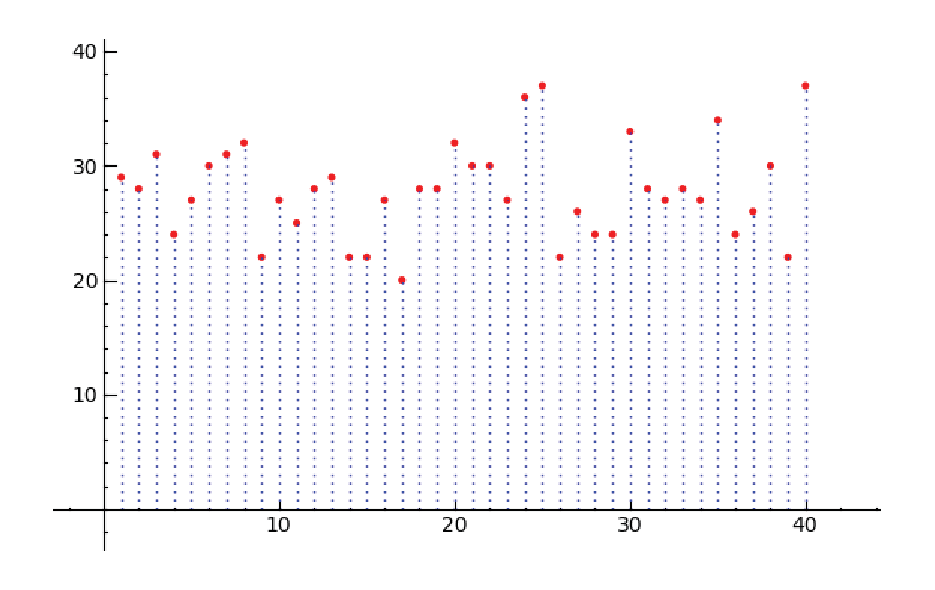
\includegraphics[width=7.5cm,height=4cm]{figures/mylotto_freq}}
\quad
\subfigure[{\scriptsize Relative frequency and probability of first ball.}]{
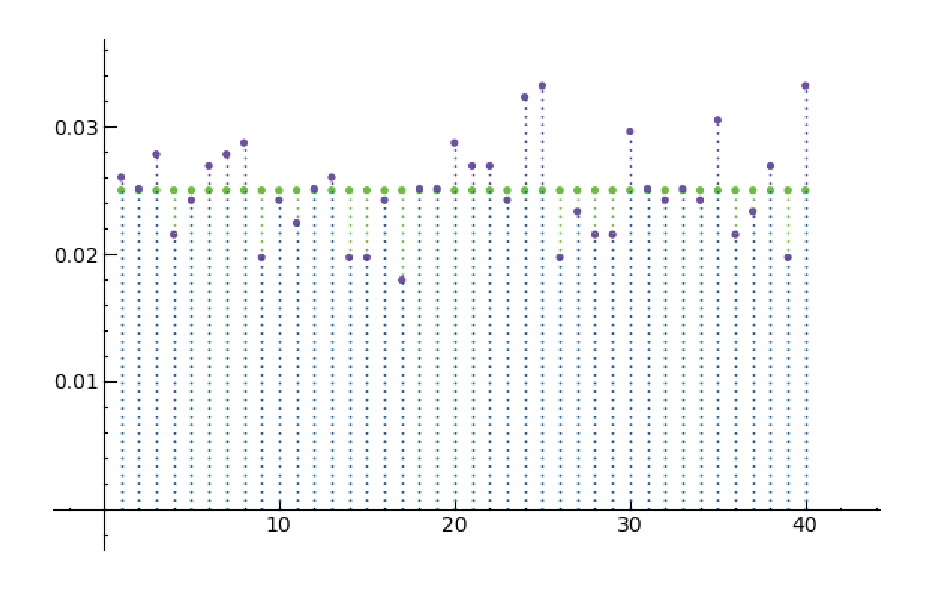
\includegraphics[width=7.5cm,height=4cm]{figures/mylotto_freq_relative}}
\caption{First ball number in 1114 NZ Lotto draws from 1987 to 2008.\label{F:LottoDraws}}
\end{figure}
\end{example}


Next, let us take a detour into how one might interpret it in the real world.  The following is an adaptation from Williams D, {\it Weighing the Odds: A Course in Probability and Statistics}, Cambridge University Press, 2001, which henceforth is abbreviated as WD2001.
\begin{center}
\begin{tabular}{l l}
{\bf Probability Model} & {\bf Real-world Interpretation} \\
Sample space $\Omega$ & Set of all outcomes of an experiment \\
Sample point $\omega$ & Possible outcome of an experiment \\ 
(No counterpart) & Actual outcome $\omega^{\star}$ of an experiment\\
Event A, a (suitable) subset of $\Omega$ & The real-world event corresponding to A \\
 & occurs if and only if $\omega^{\star} \in A$\\
$\p(A)$, a number between $0$ and $1$         & Probability that $A$ will occur for an \\
 & experiment yet to be performed \\
\\
% \end{tabular}
% \end{center}
% \begin{center}
% \begin{tabular}{l l}
{\bf Events in Probability Model} & {\bf Real-world Interpretation} \\
Sample space $\Omega$ & The certain even `something happens' \\
The $\emptyset$ of $\Omega$ & The impossible event `nothing happens' \\ 
The intersection $A \cap B$ & `Both $A$ and $B$ occur'\\
$A_1 \cap A_2 \cap \cdots \cap A_n $ & `All of the events $A_1, A_2, \ldots, A_n$ occur simultaneously'\\
The union $A \cup B$ & `At least one of $A$ and $B$ occurs'\\
$A_1 \cup A_2 \cup \cdots \cup A_n$ & `At least one of the events $A_1, A_2, \ldots, A_n$ occurs'\\
$A^c$, the complement of $A$ & `$A$ does not occur'\\
$A \setminus B$ & `$A$ occurs, but $B$ does not occur'\\
$A \subset B$ & `If $A$ occurs, then $B$ must occur'
\end{tabular}
\end{center}


{In the probability model of Example~\ref{Eg:NZLottoModel}, show that for any event $E \subset \Omega$, \[\p(E)\; =\;
\frac{1}{40} \;\times \;\text{number of elements in $E$} \enspace . \]
}
{\label{Eg:NZLottoExp}}
{
Let $E = \{\omega_1,\omega_2,\ldots,\omega_k\}$ be an event with $k$ outcomes (simple events).  
Then by the addition rule for mutually exclusive events we get:
%\begin{multiline}
$$\p(E)\;=\;\p\left( \{\omega_1,\omega_2,\ldots,\omega_k\} \right)
= \p\left(\bigcup^{k}_{i=1} \{ \omega_i \}\right)\;=\;\sum^{k}_{i=1}\p\left(\{\omega_i\}\right)\;=\;\sum^{k}_{i=1}\frac{1}{40}\;=\;\frac{k}{40} \enspace .$$

%\end{multiline}
}

\subsection{Sigma Algebras of Typical Experiments$^*$}

\begin{example}[`Toss a fair coin once']
Consider the `Toss a fair coin once' experiment.  What is its sample space $\Omega$ and a reasonable collection of events $\C{F}$ that underpin this experiment?  
\[
\Omega = \{  {\tt H}, {\tt T} \}, \qquad \C{F} = \{ {\tt H}, {\tt T},\Omega, \emptyset \} \ ,
\]
A function that will satisfy the definition of probability for this collection of events $\C{F}$ and assign $\p({\tt H}) = \frac{1}{2}$ is summarized below.  First check that the above $\C{F}$ is a sigma-algebra.  Draw a picture for $\p$ with arrows that map elements in the domain $\C{F}$ given above to elements in its range. 
\begin{center}
\begin{tabular*}{3.5in}{@{\extracolsep{\fill}}r c l} \hline
Event $A \in \C{F}$ & $\p : \C{F} \to [0,1]$ & $\p(A) \in [0,1]$ \\ \hline
$\Omega=\{ {\tt H}, {\tt T} \} \, \bullet$ & $ \ \longrightarrow \ $ & $1$ \\ 
${\tt T} \, \bullet$ & $ \ \longrightarrow \ $ & $1-\frac{1}{2}$ \\ 
${\tt H}  \, \bullet$ & $ \ \longrightarrow \ $ & $\frac{1}{2}$ \\ 
$\emptyset \, \bullet$ & $ \ \longrightarrow \ $ & $0$ \\ \hline
\end{tabular*}
\end{center}
\end{example}

\begin{classwork}[The trivial sigma algebra]
Note that $\C{F}' = \{ \Omega, \emptyset\}$ is also a sigma algebra of the sample space $\Omega= \{  {\tt H}, {\tt T} \}$.  Can you think of a probability for the collection $\C{F}'$?
\begin{center}
\begin{tabular*}{3.5in}{@{\extracolsep{\fill}}r c l} \hline
Event $A \in \C{F}'$ & $\p : \C{F}' \to [0,1]$ & $\p(A) \in [0,1]$ \\ \hline
$\Omega=\{ {\tt H}, {\tt T} \} \, \bullet$ & $ \ \longrightarrow \ $ &\\ 
$\emptyset \, \bullet$ & $ \ \longrightarrow \ $ & \\ \hline
\end{tabular*}
\end{center}
{\scriptsize
Thus, $\C{F}$ and $\C{F}'$ are two distinct sigma algebras over our $\Omega=\{ {\tt H}, {\tt T} \}$.  Moreover, $\C{F}' \subset \C{F}$ and is called a sub sigma algebra.  Try to show that $\{\Omega,\emptyset\}$ is the smallest possible sigma algebra over all possible sigma algebras over any given sample space $\Omega$ (think of intersecting an arbitrary family of sigma algebras)?
}
\end{classwork}
 
Generally one encounters four types of sigma algebras (you will understand the last two types after taking more advanced courses in mathematics, so it is fine to understand the ideas intuitively for now!) and they are:
\be
\item
When the sample space $\Omega=\{\omega_1,\omega_2,\ldots,\omega_k\}$ is a finite set with $k$ outcomes and $\p(\omega_i)$, the probability for each outcome $\omega_i \in \Omega$ is known, then one typically takes the sigma-algebra $\C{F}$ to be the set of all subsets of $\Omega$ called the {\bf power set} and denoted by $2^{\Omega}$.  
The probability of each event $A \in 2^{\Omega}$ can be obtained by adding the probabilities of the outcomes in $A$, i.e., $\p(A)=\sum_{\omega_i \in A} \p(\omega_i)$.  
Clearly, $2^{\Omega}$ is indeed a sigma-algebra and it contains $2^{\#\Omega}$ events in it.  

\item
When the sample space $\Omega=\{\omega_1,\omega_2,\ldots\}$ is a countable set then one typically takes the sigma-algebra $\C{F}$ to be the set of all subsets of $\Omega$.  Note that this is very similar to the case with finite $\Omega$ except now $\C{F}=2^{\Omega}$ could have uncountably many events in it.

%%TODO make an example of a continuous space experiment, say Darth Mole's light saber for R^1 and destination of a random ride in Doctor Who's TARDIS space-time R^d 
\item
If $\Omega = \Rz^d$ for finite $d \in \{1,2,3,\ldots\}$ then the {\bf Borel sigma-algebra} is the smallest sigma-algebra containing 
all {\bf half-spaces}, i.e., sets of the form 
$$\{x=(x_1,x_2,\ldots,x_d) \in \Rz^d: x_1 \leq c_1, x_2 \leq c_2, \ldots, x_d \leq c_d\}, \quad \text{ for any } c=(c_1,c_2,\ldots,c_d)\in\Rz^d \enspace ,
$$
When $d=1$ the half-spaces are the half-lines $\{(-\infty,c]: c \in \Rz\}$ and when $d=2$ the half-spaces are the south-west quadrants $\{(-\infty,c_1]\times(-\infty,c_2] : (c_1,c_2) \in \Rz^2\}$, etc.  
(Equivalently, the Borel sigma-algebra is the smallest sigma-algebra containing all open sets in $\Rz^d$). 

\item
Given a finite set $\Sz=\{s_1,s_2,\ldots,s_k\}$, let $\Omega$ be the sequence space $\Sz^{\infty}:=\Sz \times \Sz \times \Sz \times\cdots$, i.e., the set of sequences of infinite length that are made up of elements from $\Sz$.  
A set of the form
\[
A_1 \times A_2 \times \cdots \times A_n \times \Sz \times \Sz \times \cdots, \quad A_k \subset \Sz \text{ for all } k \in \{1,2,\ldots,n\} \enspace ,
\]
is called a {\bf cylinder set}.  
The set of events in $\Sz^{\infty}$ is the smallest sigma-algebra containing the cylinder sets. 

\begin{itemize}
\item {\bf A most primitive sigma-algebra for probability theory:} 
For example if $\Sz=\{0,1\}$, then $\Omega = \{0,1\}^{\infty}$ is the set of all infinite sequences made of $0$'s and $1$'s. 
To take advantage of arithmetic and analysis, $\Omega$ can be seen as the binary representation of all real numbers in the unit interval $[0,1]$.  
We can take advantage of combinatorics and algebra if we further represent the dyadic partition of $[0,1]$ by a binary tree (as drawn in lectures). 
Then, a cylinder set such as $1 \times 1 \times 0 \times \{0,1\} \times \{0,1\} \times \cdots$, an event here, can be interpreted as the finite binary sequence $(1,1,0)$ --- corresponding to the third leaf of a finite binary tree with four leaves obtained by splitting the right-most leaf twice. This cylindrical event $(1,1,0)$ contains all real numbers in the interval $[\frac{3}{4},\frac{7}{8}] \subset [0,1] =: \Omega$.\end{itemize}

\ee

\begin{Exercise}[title={intuiting sigma-algebra -- this is optional},label={underMPSA}]
Try to carefully recollect and understand the most primitive sigma-algebra in the last item above as it was explained in lectures.
%\ExePart
%\Question
%\subQuestion Show that...
%\subQuestion In this question...
%\subsubQuestion Show that...
%\subsubQuestion Conclude...
%\subQuestion Conclude.
%\Question Show that if $b > 1$...
%\ExePart
%\Question What happens to if $b=1$?
\end{Exercise}
\begin{Answer}
This is an optional exercise. You will understand this as you progress through your mathematics programme. 
The explanation in the said item was (or will be explained in person again) in the lectures. 
This exercise was created to answer natural questions that were asked by students who wanted to know.
\end{Answer}


\begin{framed}
PROBABILITY SUMMARY

\medskip

Axioms:
\begin{enumerate}
\item If $A\subseteq \Omega$ then $0\leq \p(A)\leq 1$ and $\p(\Omega)=1$.
\item If $A$, $B$ are disjoint events, then $\p(A\cup B)=\p(A)+\p(B)$.

[This is true only when $A$ and $B$ are disjoint.]
\item If $A_1,A_2,\dots$ are disjoint then $\p(A_1\cup A_2
\cup\dots)=\p(A_1)+\p(A_2)+\dots$
\end{enumerate}
Rules:
$$\p(A^c)\;=\;1-\p(A)$$
$$\p(A\cup B)\;=\;\p(A)+\p(B)-\p(A\cap B) \qquad [\textrm{always true}]$$
\end{framed}

\section{Exercises in Probability}\label{S:xsProbability}

\begin{ExerciseList}
\Exercise
{In English language text, the twenty six letters in the alphabet occur with the following frequencies:
{\footnotesize $$
\mathsf{
\begin{array}{cccccccccccccccccc}
\sf E   &       13      \%&     \sf R   &       7.7     \%&     \sf A   &       7.3     \%&     \sf H   &       3.5     \%&     \sf F   &       2.8     \%&     \sf M    &      2.5     \%&     \sf W   &       1.6     \%&     \sf X   &       0.5     \%&     \sf J   &       0.2     \%\\
\sf T   &       9.3     \%&     \sf O   &       7.4     \%&     \sf S   &       6.3     \%&     \sf L   &       3.5     \%&     \sf P   &       2.7     \%&     \sf Y    &      1.9     \%&     \sf V   &       1.3     \%&     \sf K   &       0.3     \%&     \sf Z   &       0.1     \%\\
\sf N   &       7.8     \%&     \sf I   &       7.4     \%&     \sf D   &       4.4     \%&     \sf C   &       3       \%&     \sf U   &       2.7     \%&     \sf G    &      1.6     \%&     \sf B   &       0.9     \%&     \sf Q   &       0.3     \%&             &               \\
\end{array}
}
$$}
Suppose you pick one letter at random from a randomly chosen English
book from our central library with
$\Omega=\{\mathsf{A,B,C,\ldots,Z}\}$ (ignoring upper/lower cases),
then what is the probability of these events?
\begin{itemize}
\item[(a)]$\p(\{\mathsf{Z}\})$
\item[(b)]$\p(\textrm{`picking any letter'})$
\item[(c)] $\p(\{\mathsf{E},\mathsf{Z}\})$
\item[(d)]$\p(\textrm{`picking a vowel'})$
\item[(e)]$\p(\textrm{`picking any letter in the word WAZZZUP'})$
\item[(f)]$\p(\textrm{`picking any letter in the word WAZZZUP or a vowel'})$.
\end{itemize}
}
\label{Ex:RandomEnglishLetter}
\Answer
{\bit
\item[(a)] $\p(\{\mathsf{Z}\})=0.1\%=\frac{0.1}{100}=0.001$
\item[(b)] $\p(\textrm{`picking any letter'})= \p(\Omega) = 1$
\item[(c)] $\p(\{\mathsf{E},\mathsf{Z}\}) =\p(\{\mathsf{E}\} \cup
    \{\mathsf{Z}\} ) =  \p(\{\mathsf{E}\})+\p(\{\mathsf{Z}\}) =
    0.13+0.001=0.131$, by Axiom~(3)
\item[(d)] $\p(\textrm{`picking a
    vowel'})=\p(\{\mathsf{A,E,I,O,U}\})=(7.3\%+13.0\%+7.4\%+7.4\%+2.7\%)=37.8\%$,  by the addition rule for mutually exclusive events, rule (2).
\item[(e)] $\p(\textrm{`picking any letter in the word
    WAZZZUP'})=\p(\{\mathsf{W,A,Z,U,P}\})=14.4\%$,  by the
  addition rule for mutually exclusive events, rule (2).
\item[(f)] $\p(\textrm{`picking any letter in the word WAZZZUP or a vowel'})=$\\
$\p(\{\mathsf{W,A,Z,U,P}\})+\p(\{\mathsf{A,E,I,O,U}\})-\p(\{\mathsf{A,U}\})
  = 14.4\% + 37.8\% - 10\% = 42.2\%$,  by the addition rule for two
arbitrary events, rule (3).
\eit
}


\Exercise
Find the sample spaces  for the following experiments:
\begin{enumerate}
\item Tossing 2 coins whose faces are sprayed with black paint denoted by $\mathsf{B}$ and white paint denoted by $\mathsf{W}$.
\item Drawing 4 screws from a bucket  of left-handed and right-handed screws
  denoted by $\mathsf{L}$ and $\mathsf{R}$, respectively.
\item Rolling a die and recording the number on the upturned face  until the first $\mathsf{6}$ appears.
\end{enumerate}
\Answer
\be
\item $\{\mathsf{BB},\mathsf{BW},\mathsf{WB},\mathsf{WW}\}$

\item $\begin{aligned}\{\mathsf{ RRRR,RRRL,RRLR,RLRR,LRRR,RLRL,RRLL,LLRR,}
    \\ \mathsf{LRLR,LRRL,RLLR,LLLL, LLLR,LLRL,LRLL,RLLL}\}\end{aligned}$
\item $\{6,16,26,36,46,56,116, 126,136, 146, 156,
      216, 226, 236, 246, 256, \,\ldots\}$
\ee


\Exercise
Suppose we pick a letter at random from the word WAIMAKARIRI. 
\begin{enumerate}
\item What is the sample space $\Omega$?
\item  What probabilities should be assigned to the outcomes?
\item What is the probability of {\emph not} choosing the letter  R?
\end{enumerate}
\Answer

\be
\item The sample space $\Omega=\{\mathsf{W},\mathsf{A},\mathsf{I},\mathsf{M},\mathsf{K},\mathsf{R}\}$.
\item   Since there are eleven letters in WAIMAKARIRI the probabilities are:
\cen{ $\p(\sf\{W\})=\frac{1}{11}$, $\p(\sf\{ A\})=\frac{3}{11}$, $\p( \sf\{ I\})
=\frac{3}{11}$,
    $\p(\sf\{ M\})=\frac{1}{11}$, $\p(\sf\{ K\})=\frac{1}{11}$, $\p(\sf\{
    R\})=\frac{2}{11}$\,.}

\item By the complementation rule, the probability of not choosing
    the letter R is:  \[1\,-\,\p(\text{choosing the letter R})\,=\,1\,-\, \frac{2}{11}\,=\,\frac{9}{11}\,.\]

\ee


\Exercise
There are seventy five balls in total inside the Bingo Machine.  
Each ball is labelled by one of the following five letters: 
$\mathsf{B}$, $\mathsf{I}$, $\mathsf{N}$, $\mathsf{G}$, and $\mathsf{O}$.  
There are fifteen balls labelled by each letter.  
The letter on the first ball that comes out of a BINGO machine after it has been well-mixed is the outcome of our experiment. 
\begin{itemize}
\item[(a)] Write down the sample space of this experiment.
\item[(b)] Find the probabilities of each simple event.
\item[(c)] Show that $\p(\Omega)$ is indeed $1$.
\item[(d)] Check that the addition rule for mutually exclusive events holds for the simple events $\{B\}$ and $\{I\}$. 
\item[(e)]Consider the following events: 
$C = \{\mathsf{B},\mathsf{I},\mathsf{G}\}$ and $D = \{\mathsf{G},\mathsf{I},\mathsf{N}\}$.  
Using the addition rule for two arbitrary events, find  $\p(C \cup D)$.
\end{itemize}

\Answer
\be
\item
First, the sample space is: $\Omega=\{ {\mathsf{B}, \mathsf{I},
  \mathsf{N}, \mathsf{G}, \mathsf{O} } \} \enspace . $
\medskip

\item The probabilities of simple events are:
$$
\p(\mathsf{B} )\;=\;\p(\mathsf{I})\;=\;\p(\mathsf{N})\;=\;\p(\mathsf{G})\;=\;\p(\mathsf{O})\;=\;{\frac{15}{75}\;=\;\frac{1}{5}} \enspace .
$$

\item 

%Axiom~(1):
%$${0\leq \p(\mathsf{B})\;=\;\p(\mathsf{I})\;=\;\p(\mathsf{N})\;=\;\p(\mathsf{G})\;=\;\p(\mathsf{O})\;=\;\frac{1}{5} \leq 1 \enspace .}
%$$

%Axiom~(2): 
Using the addition rule for mutually exclusive events,
\begin{eqnarray*}
\p(\Omega)
&=& \p(\mathsf{\{B,I,N,G,O\}})\\
&=& \p(\{\sf{B}\} \cup\{\sf{I}\}\cup \{\sf{N}\} \cup \{\sf{G}\} \cup \{\sf{O}\})\\
&=& \p(\sf B)+\p(\sf I)+\p(\sf N)+\p(\sf G)+\p(\sf O) \quad \text{simplifying notation} \\
&=& \frac{1}{5}+\frac{1}{5}+\frac{1}{5}+\frac{1}{5}+\frac{1}{5}\\
&=& 1
\end{eqnarray*}

\item Since the   events $\{\sf B\}$ and $\{\sf I\}$ are disjoint,
$$
\p(\{\sf{B}\} \cup \{\sf{I}\})\;=\;\p(\sf B)+\p(\sf I)\;=\;\frac{1}{5}+\frac{1}{5}\;=\;\frac{2}{5}\,.
$$


\medskip


\item  Using the addition rule for two arbitrary events we get,
\begin{eqnarray*}
\p(C \cup D) &=& \p(C)+\p(D)-\p(C\cap D)\\& =& \p(\{\sf{B},\sf{I},\sf{G}\}) + \p(\{\sf{G},\sf{I},\sf{N}\}) - \p(\{\sf{G},\sf{I}\})\\
& =& \frac{3}{5} +\frac{3}{5} - \frac{2}{5}\\& = &\frac{4}{5} \enspace .
\end{eqnarray*}
\ee


\end{ExerciseList}



\section{Conditional Probability}\label{S:CondProb}
Next, we define conditional probability and the notion of independence of events.  We use the LTRF idea to motivate the definition.
\begin{idea}[LTRF intuition for conditional probability]
Let $A$ and $B$ be any two events associated with our experiment $\E{E}$ with $\p(A) \neq 0$.  The `conditional probability that $B$ occurs given that $A$ occurs' denoted by $\p(B|A)$ is again intuitively underpinned by the super-experiment $\E{E}^{\infty}$ which is the `independent' repitition of our original experiment $\E{E}$ `infinitely' often.  The LTRF idea is that $\p(B|A)$ is the long-term proportion of those experiments on which $A$ occurs that $B$ also occurs.
 
Recall that $N(A,n)$ as defined in \eqref{E:NofAn} is the fraction of times $A$ occurs out of $n$ independent repetitions of our experiment $\E{E}$ (ie.~the experiment $\E{E}^{n}$).  If $A \cap B$ is the event that `$A$ and $B$ occur simultaneously', then we intuitively want
\[
\p(B|A) \quad \lq\lq \rightarrow " \quad \frac{N(A \cap B,n)}{N(A,n)} = \frac{N(A \cap B,n)/n}{N(A,n)/n} =  \frac{\p(A \cap B)}{\p(A)}
\]
as our $\E{E}^{n} \rightarrow \E{E}^{\infty}$.  So, we {\bf define} conditional probability as we want.
 \end{idea}
 \begin{definition}[Conditional Probability]\label{D:CondProb}
Suppose we are given an experiment $\E{E}$ with a triple $(\Omega, \C{F}, \p)$.  Let $A$ and $B$ be events, ie.~$A,B \in \C{F}$, such that $\p(A) \neq 0$.  Then, we define the {\bf conditional probability} of $B$ given $A$ by,
 \begin{equation}\label{E:CPD}
 \p(B|A) := \frac{\p(A \cap B)}{\p(A)} \ .
 \end{equation}
 Note that for a {\bf fixed} event $A \in \C{F}$ with $\p(A)>0$ and {\bf any} event $B \in \C{F}$, the conditional  probability $\p(B | A)$ is a probability as in \hyperref[D:Prob]{Definition \ref*{D:Prob}}, ie.~a function:
 \[
 \p(B | A) : \C{F} \rightarrow [0,1]
 \]
 that assigns to each $B \in \C{F}$ a number in the interval $[0,1]$, such that,
 \begin{enumerate}
 \item $\p(\Omega | A) = 1$ \qquad Meaning `Something Happens given the event A happens'
 \item The `Addition Rule' axiom holds, ie.~for events $B_1, B_2 \in \C{F}$,
 \[
 B_1 \cap B_2 = \emptyset \quad \text{implies} \quad \p(B_1 \cup B_2 | A) = \p(B_1 | A) + \p(B_2 |  A)  \ .
 \]

\item For mutually exclusive or pairwise-disjoint events, $B_1,B_2, \ldots$,
\[
\p(B_1 \cup B_2 \cup \cdots | A) = \p(B_1|A)+\p(B_2|A)+\cdots \enspace .
\]
\end{enumerate} 
\end{definition}

From the definition of conditional probability we get the following rules:
\be
\item Complementation rule: $\p(B | A)\, = \,1 - \p(B^c | A)$ .

\item Addition rule for two arbitrary events $B_1$ and $B_2$: \[{\p(B_1 \cup B_2 | A) \;= \;\p(B_1 | A) + \p(B_2 | A) - \p(B_1\cap B_2|A)}\,.\]

\item Multiplication rule for two likely events: 

If $A$ and $B$ are events, and if
  $\p(A)\neq 0$ and  $\p(B)\neq 0$, then
\[\p(A\cap B)\;=\;\p(A)\p(B|A)\;=\;\p(B)\p(A|B)\,. \]
\ee

\begin{example}[Wasserman03, p.~11]\label{EX:Wasserman03p11}
 A medical test for a disease $D$ has outcomes $+$ and $-$.  the probabilities are:
\begin{center}
 \begin{tabular}{l | c | c}
 \hline
 & Have Disease ($D$) & Don't have disease ($D^c$)  \\ \hline
Test positive ($+$) & 0.009 & 0.099 \\
 Test negative ($-$) & 0.001 & 0.891\\ \hline
 \end{tabular}
 \end{center}
 Using the definition of conditional probability, we can compute the conditional probability that you test positive given that you have the disease:
 \[
 \p(+ | D) = \frac{\p(+ \cap D)}{\p(D)} = \frac{0.009}{0.009+0.001}=0.9 \ ,
 \]
 and the conditional probability that you test negative given that you don't have the disease:
 \[
 \p(- | D^c) = \frac{\p(- \cap D^c)}{\p(D^c)} = \frac{0.891}{0.099+0.891} \approxeq 0.9 \ .
 \]
 Thus, the test is quite accurate since sick people test positive 90\% of the time and healthy people test negative 90\% of the time.
 
Now, suppose you go for a test and and test positive.  What is the probability that you have the disease ?
 \[
 \p(D|+) = \frac{\p(D \cap +)}{\p(+)} = \frac{0.009}{0.009+0.099} \approxeq 0.08
 \]
Most people who are not used to the definition of conditional probability would intuitively associate a number much bigger than $0.08$ for the answer.  Interpret conditional probability in terms of the meaning of the numbers that appear in the numerator and denominator of the above calculations.
\end{example}
 
\subsection{Bayes' Theorem}\label{S:BayesTheorem}
 Next we look at one of the most elegant applications of the definition of conditional probability along with the addition rule for a partition of $\Omega$.
 \begin{prop}[Bayes' Theorem, 1763]
 Suppose the events $A_1,A_2,\ldots,A_k \in \C{F}$, with $\p(A_h)>0$ for each $h \in \{1,2,\ldots,k\}$, partition the sample space $\Omega$, ie.~they are mutually exclusive (disjoint) and exhaustive events with positive probability: 
 \[
 A_i \cap A_j = \emptyset, \ \text{for any distinct $i,j \in \{1,2,\ldots,k\}$}, \qquad \bigcup_{h=1}^k A_h = \Omega, \qquad \p(A_h) > 0
 \]
 Thus, precisely one of the $A_h$'s will occur on any performance of our experiment $\E{E}$.  
 
 Let $B \in \C{F}$ be some event with $\p(B) > 0$, then 
 \begin{equation}\label{E:BayesThm}
 \p(A_h|B) = \frac{\p(B|A_h) \p(A_h)}{\sum_{h=1}^k \p(B|A_h) \p(A_h)}
 \end{equation}
 {\scriptsize
 \begin{proof}
 We apply elementary set theory, the definition of conditional probability $k+2$ times and the addition rule once:
 \begin{eqnarray}
 \p(A_h | B) &=& \frac{\p(A_h \cap B)}{\p(B)} = \frac{\p( B \cap A_h)}{\p(B)} = 
 \frac{\p( B | A_h) \p(A_h)}{\p(B)}  \notag \\
 &=& \frac{\p( B | A_h) \p(A_h)}{\p \left( \bigcup_{h=1}^k (B \cap A_h) \right)} =
 \frac{\p( B | A_h) \p(A_h)}{\sum_{h=1}^k \p \left( B \cap A_h \right)} \notag \\
 &=& \frac{\p( B | A_h) \p(A_h)}{\sum_{h=1}^k \p(B | A_h) \p(A_h)} \notag
 \end{eqnarray}
 \end{proof}
}
The operations done to the denominator in the proof above:
\begin{equation}\label{E:LTP}
\p( B) = \sum_{h=1}^k \p(B | A_h) \p(A_h)
\end{equation}
is also called `the law of total probability' or `the total probability theorem'.  
We call $\p(A_h)$ the {\bf prior probability of} $A_h$ and $\p(A_h|B)$ the {\bf posterior probability of} $A_h$.
 \end{prop}

\begin{example}[Wasserman2003~p.12]\label{Wasserman2003p12}
Suppose Larry divides his email into three categories: $A_1 = \text{``spam''}$, $A_2 =\text{ ``low priority''}$, and $A_3 = \text{ ``high priority''}$.  From previous experience, he finds that $\p(A_1) = 0.7$, $\p(A_2) = 0.2$ and $\p(A_3)=0.1$.  Note that $\p(A_1 \cup A_2 \cup A_3) = \p(\Omega) = 0.7+0.2+0.1 = 1$.  Let $B$ be the event that the email contains the word ``free.''  From previous experience, $\p(B|A_1) = 0.9$, $\p(B|A_2) = 0.01$ and $\p(B|A_3)=0.01$.  Note that $\p(B|A_1) + \p(B|A_2) + \p(B|A_3) = 0.9+0.01+0.01 \neq 1$.  Now, suppose Larry receives an email with the word ``free.''  What is the probability that it is ``spam,'' ``low priority,''  and ``high priority'' ?
%{\color{Gray}{

{\scriptsize{
\[
\begin{array}{l l l l l}
\p(A_1 | B) 
&= \frac{\p(B|A_1)\p(A_1)}{\p(B|A_1)\p(A_1)+\p(B|A_2)\p(A_2)+\p(B|A_3)\p(A_3)} 
&= \frac{0.9 \times 0.7}{(0.9 \times 0.7)+ (0.01 \times 0.2) + (0.01 \times 0.1)}
&= \frac{0.63}{0.633}
&\approxeq 0.995 \\
\\
\p(A_2 | B) 
&= \frac{\p(B|A_2)\p(A_2)}{\p(B|A_1)\p(A_1)+\p(B|A_2)\p(A_2)+\p(B|A_3)\p(A_3)} 
&= \frac{0.01 \times 0.2}{(0.9 \times 0.7)+ (0.01 \times 0.2) + (0.01 \times 0.1)}
&= \frac{0.002}{0.633}
&\approxeq 0.003 \\
\\
\p(A_3 | B) 
&= \frac{\p(B|A_3)\p(A_3)}{\p(B|A_1)\p(A_1)+\p(B|A_2)\p(A_2)+\p(B|A_3)\p(A_3)} 
&= \frac{0.01 \times 0.1}{(0.9 \times 0.7)+ (0.01 \times 0.2) + (0.01 \times 0.1)}
&= \frac{0.001}{0.633}
&\approxeq 0.002 \\
\end{array}
\]
Note that $\p(A_1|B) + \p(A_2|B)+\p(A_3|B) = 0.995+0.003+0.002=1$.
}}
%}}
\end{example}

\begin{example}[Urn with red and black balls]\label{EX:urnRedBlackBalls} 
A well-mixed urn contains five
{\sf red} and ten {\sf black} balls. We draw two balls from the urn
without replacement. What is the probability that the second ball drawn
is {\sf red}?

This is easy to see if we draw a probability tree diagram.  
The first split in the tree is based on the outcome of the first draw and the second on the outcome of the last draw.  
The outcome of the first draw dictates the probabilities for the second one since we are sampling without replacement.  
We multiply the probabilities on the edges to get probabilities of the four endpoints, and then sum the ones that correspond to {\sf red} in the second draw, that is
\[
P(\text{second ball is red}) \;=\; 4/42+10/42\;=\;1/3 \enspace .
\]

\begin{center}
\begin{picture}(100,140)(75,30)
\drawline(0,90)(75,120)(125,140)
\drawline(75,120)(125,100)
\drawline(0,90)(75,60)(125,40)
\drawline(75,60)(125,80)
\put(55,125){{\sf red}}\put(55,45){{\sf black}}
\put(130,140){$\mathsf{(red, red)}$ 4/42}\put(130,100){$\mathsf{(red, black)}$ 10/42}
\put(130,80){$\mathsf{(black, red)}$ 10/42}\put(130,40){$\mathsf{(black, black)}$ 18/42}
\put(95,140){4/14}\put(95,115){10/14}
\put(95,80){5/14}\put(95,55){9/14}
\put(30,110){1/3}\put(30,80){2/3}
\end{picture}
\end{center}

Alternatively,  use the total probability theorem to break
the problem  down into manageable pieces.  
Let
  $R_1=\{\mathsf{(red,red),(red,black)}\}$ and
  $R_2=\{\mathsf{(red,red),(black,red)}\}$ be the events corresponding
  to a {\sf red} ball in the $1$st and $2$nd draws, respectively, and
  let $B_1=\{\mathsf{(black,red),(black,black)}\}$ be the event of a
  {\sf black} ball on the first draw.

Now $R_1$ and $B_1$ partition $\Omega$ so we can  write:
\begin{eqnarray*}
P(R_2)
&=& \p(R_2\cap R_1) + \p(R_2\cap B_1)\\[6pt]
&=& \p\;(R_2| R_1)\p(R_1) + \p(R_2|B_1)\p(B_1)\\[6pt]
&=& (4/14)(1/3)\,+\,(5/14)(2/3) =  1/3 \enspace .
\end{eqnarray*}
\end{example}

 \subsection{Independence and Dependence}\label{S:IndepDep}
 \begin{definition}[Independence of two events]\label{D:IndOf2Events}
 Any two events $A$ and $B$ are said to be {\bf independent} if and only if
 \begin{equation}\label{E:PofAB=PAPB}
 \p(A \cap B) = \p(A) \p(B) \ .
 \end{equation}
 \end{definition}
 Let us make sense of this definition in terms of our previous definitions.  When $\p(A)=0$ or $\p(B)=0$, both sides of the above equality are $0$.  If $\p(A) \neq 0$, then rearranging the above equation we get:
 \[
 \frac{\p(A \cap B)}{\p(A)} = \p(B) \ .
 \]
 But, the LHS is $\p(B|A)$ by \hyperref[E:CPD]{definition \ref*{E:CPD}}, and thus for independent events $A$ and $B$, we get:
 \[
 \p(B|A) = \p(B) \ .
 \]
This says that information about the occurrence of $A$ does not affect the occurrence of $B$.  If $\p(B) \neq 0$, then an analogous argument:
{\scriptsize
\[
\p(A \cap B) = \p(A) \p(B) \iff \p(B \cap A) = \p(A) \p(B) \iff \frac{\p(B \cap A)}{\p(B)} = \p(A) \iff  \p(A|B) = \p(A) \ ,
\]
}
says that information about the occurrence of $B$ does not affect the occurrence of $A$.  Therefore, the probability of their joint occurence $\p(A \cap B)$ is simply the product of their individual probabilities $\p(A) \p(B)$.

\begin{definition}[Independence of a sequence of events]\label{D:IndOfSeqOfEvents}
We say that a finite or infinite sequence of events $A_1,A_2,\ldots$ are independent if whenever $i_1,i_2,\ldots,i_k$ are distinct elements from the set of indices $\Nz$, such that $A_{i_1},A_{i_2},\ldots,A_{i_k}$ are defined (elements of $\C{F}$), then
\[
\p(A_{i_1} \cap A_{i_2} \ldots \cap A_{i_k})  =  \p(A_{i_1} ) \p(A_{i_2})  \cdots \p(A_{i_k}) 
\]
\end{definition}

\begin{example}[Some Standard Examples]
A sequence of events in a sequence of independent trials is independent.
\be

\item[(a)] Suppose you toss a fair coin twice such that the first toss is independent of the second.  Then,
$$
\p(\mathsf{Heads} \text{ on the first toss} \cap \mathsf{Tails} \text{ on the second toss} ) = \p(\mathsf{H}) \p(\mathsf{T}) = \frac{1}{2} \times \frac{1}{2}= \frac{1}{4} \enspace .
$$

\item[(b)] Suppose you independently toss a fair die three times.  Let $E_i$ be the event that the outcome is an even number on the $i$-th trial.  The probability of getting an even number in all three trials is:
\begin{eqnarray*}
\p(E_1 \cap E_2 \cap E_3)
&=& \p(E_1) \p(E_2) \p(E_3)\\
&=& \left(\p(\{\mathsf{2,4,6}\})\right)^3\\
&=& \left(\p(\{\mathsf{2}\} \cup \{\mathsf{4}\} \cup \{\mathsf{6}\}) \right)^3 \\
&=& \left(\p(\{\mathsf{2}\}) + \p(\{\mathsf{4}\}) + \p(\{\mathsf{6}\})\right)^3\\
&=& \left(\frac{1}{6} + \frac{1}{6} + \frac{1}{6} \right)^3 
= \left(\frac{1}{2} \right)^3
= \frac{1}{8} \enspace .
\end{eqnarray*}
%This is an obvious answer but there is a lot of maths going on here!

\item[(c)]Suppose you toss a fair coin independently $m$ times.  Then each of the $2^m$ possible outcomes in the sample space $\Omega$ has equal probability of $\frac{1}{2^m}$ due to independence.
\ee
\end{example}

\begin{example}[dependence and independence] 
Suppose we toss two fair dice.  
Let $A$ denote the event that the sum of the dice is six and $B$ denote the event that the first die equals four.  The sample space encoding the thirty six ordered pairs of outcomes for the two dice is $\Omega = \{ (1,1), (1,2), \ldots, (1,6), (2,1), \ldots, (2,6), \ldots, (5,6), (6,6)\}$ and due to independence $\p(\omega)=1/36$ for each $\omega\in\Omega$.  
Then 
\[
\p(A \cap B)  = \p (\{(4,2)\}) = \frac{1}{36} \enspace ,
\]
but
\begin{eqnarray*}
\p(A)\p(B) 
&=& \p (\{(1,5),(2,4),(3,3),(4,2),(5,1)\}) \p( \{ (4,1),(4,2),(4,3),(4,4),(4,5),(4,6) \}) \\
&=& \frac{5}{36}\times \frac{6}{36} = \frac{5}{36}\times\frac{1}{6} = \frac{5}{216} \enspace ,
\end{eqnarray*}
and therefore $A$ and $B$ are not independent.  
The reason for the events $A$ and $B$ being dependent is clear because the chance of getting a total of six depends on the outcome of the first die (not being six).

Now, let $C$ be the event that the sum of the two dice equals seven.  
Then
\[
\p(C \cap B)  = \p (\{(4,3)\}) = \frac{1}{36} \enspace ,
\]
while
\begin{eqnarray*}
\p(C \cap B)  
&=& \p (\{(1,6),(2,5),(3,4),(4,3),(5,2),(6,1)\}) \p( \{ (4,1),(4,2),(4,3),(4,4),(4,5),(4,6) \})\\
&=& \frac{6}{36}\times\frac{6}{36}= \frac{1}{36} \enspace ,
\end{eqnarray*}
and therefore $C$ and $B$ are independent events.  Once again this is clear because the chance of getting a total of seven does not depend any more on the outcome of the first die (it is allowed to be any one of the six possible outcomes). 
\end{example}

\begin{example}[Pairwise independent events that are not jointly independent]
Let a ball be drawn from an well-stirred urn containing four balls labelled 1,2,3,4.  
Consider the events $A = \{1,2\}$, $B=\{1,3\}$ and $C=\{1,4\}$.  
Then,
\begin{eqnarray*}
\p(A \cap B) &=& \p(A)\p(B) = \frac{2}{4}\times\frac{2}{4} = \frac{1}{4},\\
\p(A \cap C) &=& \p(A)\p(C) = \frac{2}{4}\times\frac{2}{4} = \frac{1}{4},\\
\p(B \cap C) &=& \p(B)\p(C) = \frac{2}{4}\times\frac{2}{4} = \frac{1}{4},
\end{eqnarray*}
but,
\[
\frac{1}{4} = \p(\{1\}) = \p (A \cap B \cap C) \neq \p(A)\p(B)\p(C) = \frac{2}{4}\times\frac{2}{4}\times\frac{2}{4}=\frac{1}{8} \enspace .
\]
Therefore, inspite of being pairwise independent, the events $A$, $B$ and $C$ are not jointly independent.
\end{example}

\begin{framed}
CONDITIONAL PROBABILITY SUMMARY\\

$\p(A|B)$ means the probability that $A$ occurs given that $B$ has
occurred.

$$\p(A|B)\;=\;\frac{\p(A\cap B)}{\p(B)}\;=\;\frac{\p(A)\p(B|A)}{\p(B)}\quad \textrm{if}\quad \p(B)\neq0$$

$$\p(B|A)\;=\;\frac{\p(A\cap B)}{\p(A)}\;=\;\frac{\p(B)\p(A|B)}{\p(A)}\quad \textrm{if}\quad \p(A)\neq 0$$

Conditional probabilities obey the axioms and rules of probability.
\end{framed}

\section{Exercises in Conditional Probability}\label{S:xsCondProb}

\begin{ExerciseList}

\Exercise
What gives the greater probability of hitting some target at least
  once: 
\begin{enumerate}
\item  hitting in a shot with probability $\frac{1}{2}$ and firing 1 shot, or 
\item hitting in a shot with probability $\frac{1}{3}$ and firing 2 shots?
\end{enumerate}
First guess. Then calculate.

\Answer
We can assume  that the first shot is independent of
the second shot so we can multiply the probabilities here.

For case A, there is only one shot so the probability of hitting at least once is $\frac{1}{2}$.

For case B, the probability of missing both shots is
$\frac{2}{3}\,\frac{2}{3}\,=\,\frac{4}{9}$,  so  the probability hitting some target at least once is
  \[ 1- \p(\text{missing the target both times})\;=\; 1-\frac{4}{9}\;=\;\frac{5}{9}\]
Therefore, case B has the greater probability of hitting the target at least once.

\Exercise
Suppose we independently roll two fair dice each of whose faces are marked by numbers
  $\sf 1$,$\sf 2$,$\sf 3$,$\sf 4$, $\sf 5$ and $\sf 6$.
\begin{enumerate}
\item List the sample space for the experiment if we note the   numbers
  on the 2 upturned faces.
\item What is the probability of obtaining a sum greater than 4 but less
  than 7?
\end{enumerate}

\Answer
\be
\item The sample space is
$$
\begin{aligned}
\{
\mathsf{(1,1),(1,2),(1,3),(1,4),(1,5),(1,6),\quad (2,1),(2,2),(2,3),(2,4),(2,5),(2,6),}\\
\mathsf{(3,1),(3,2),(3,3),(3,4),(3,5),(3,6),\quad (4,1),(4,2),(4,3),(4,4),(4,5),(4,6),}\\
\mathsf{(5,1),(5,2),(5,3),(5,4),(5,5),(5,6),\quad (6,1),(6,2),(6,3),(6,4),(6,5),(6,6)}
\}
\end{aligned}
$$
Note: Order matters here. For example, the outcome ``16'' refers to a ``1'' on the first die and a ``6'' on the second,
whereas the outcome ``61'' refers to a ``6'' on the first die and a ``1'' on the
second.

\item First tabulate all possible sums as follows:
$$
\begin{array}{c|cccccc}
+       &       1       &       2       &       3       &       4       &       5       &       6       \\\hline
1       &       2       &       3       &       4       &       \mathbf{5}      &       \mathbf{6}      &       7       \\
2       &       3       &       4       &       \mathbf{5}      &       \mathbf{6}      &       7       &       8       \\
3       &       4       &       \mathbf{5}      &       \mathbf{6}      &       7       &       8       &       9       \\
4       &       \mathbf{5}      &       \mathbf{6}      &       7       &       8       &       9       &       10      \\
5       &       \mathbf{6}      &       7       &       8       &       9       &       10      &       11      \\
6       &       7       &       8       &       9       &       10      &       11      &       12      \\
\end{array}$$
 Let $A$ be the event {\em the sum is 5} and $B$ be the event {\em
    the sum is 6}, then $A$ and $B$ are mutually exclusive events with
  probabilities \[\p(A) = \frac{4}{36} \quad \text{and}\quad \p(B) =
  \frac{5}{36} \,.\]
Therefore,
   $$\p(4<\textrm{sum }<7)\;=\; \p( A \cup B) \;=\; \p(A)\,+\,\p(B)\;=\; \frac{4}{36} +
\frac{5}{36} \;=\;\frac{1}{4}$$
\ee


\Exercise
Based on past experience, 70\% of students in a certain course pass the midterm test.  
The final exam is passed by 80\% of those who passed the midterm test, but only by 40\% of those who fail the midterm test.  
What fraction of students pass the final exam?

\Answer
First draw a tree  with the first split based on the outcome of the midterm test and the second on the outcome of the final exam.  
Note that the probabilities involved in this second branch are {\em conditional} probabilities that depend on the outcome of the midterm test.  
Let $A$ be the event that the student passes the final exam and let $B$ be the event that the student passes the midterm test.

\begin{center}
\begin{picture}(100,160)(75,30){\drawline(0,90)(75,120)(125,140)
\drawline(75,120)(125,100)\drawline(0,90)(75,60)(125,40)
\drawline(75,60)(125,80)
\put(55,125){$B$}\put(55,50){$B^c$}
\put(130,140){$A$\quad $\p(A \cap  B) = 0.56$}\put(130,100){$A^c$ \quad
  $\p(A^c\cap B)= 0.14$}
\put(130,80){$A$ \quad $\p(A\cap B^c) = 0.12$ }\put(130,40){$A^c$ \quad
  $\p(A^c\cap B^c)= 0.18$}
\put(100,137){0.8}\put(100,112){0.2}
\put(100,77){0.4}\put(100,52){0.6}
\put(30,110){0.7}\put(30,85){0.3}}
\put(40,165){Midterm}
\put(120,165){Final}
\end{picture}
\end{center}

Then the probability of passing the final exam is:
\[ \p(A)\;=\; 0.56\,+\,0.12\;=\;0.68\,.\]

To do this with formulae,  partitioning according to the midterm test
result  and using the multiplication rule, we get:
\begin{eqnarray*}
\p(A)&=& \p(A\cap B)+\p(A\cap B^c)\\
&=& \p(A|B)\p(B)+\p(A|B^c)\p(B^c)\\
&=& (0.8)(0.7)+(0.4)(0.3)\;=\;0.68
\end{eqnarray*}

\Exercise
A small brewery has two bottling machines.  
Machine 1 produces 75\% of the bottles and machine 2 produces 25\%.  
One out of every 20 bottles filled by machine 1 is rejected for some reason, while one out of every 30 bottles filled by machine 2 is rejected. 
What is the probability that a randomly selected bottle comes from machine 1 given that it is accepted?
\Answer
Let $A$ be the event that bottles are produced by machine 1; and $A^c$ is the event that bottles are produced by machine 2. 
$R$ denotes the event that the bottles are rejected; and $R^c$ denotes the event that the bottles are accepted.  
We know the following probabilities:

\[ \p(A) \;=\; 0.75 \quad \text{and} \quad \p(A^c) \;=\; 0.25\]
\[ \p(R | A) \;=\; \frac{1}{20} \quad \text{and } \quad  \p(R^c | A) \;=\;
\frac{19}{20}\]

\[ \p(R | A^c) \;=\; \frac{1}{30} \quad \text{and} \quad  \p(R^c | A^c) \;=\;
\frac{29}{30}\]

We want $\p(A|R^c)$ which is give by
$$\p(A|R^c)\;=\;\frac{\p(R^c\cap A)}{\p(R^c)}\;=\;\frac{\p(R^c\cap A)}{\p(R^c\cap A)+\p(R^c\cap A^c)}$$
where, $$\p(R^c\cap A)\;=\;\p(R^c| A)\p(A)\;=\;\frac{19}{20}\times0.75$$
and, $$\p(R^c\cap A^c)\;=\;\p(R^c|A^c)\p(A^c)\;=\;\frac{29}{30}\times0.25$$
Therefore,
$$\p(A|R^c)\;=\;\frac{\frac{19}{20}\times0.75}{\frac{19}{20}\times
  0.75+\frac{29}{30}\times0.25}\;\approxeq \;0.747\quad $$\\[6pt]

The  tree diagram for this problem is:
\begin{center}
\begin{picture}(100,140)(75,30){\drawline(0,90)(75,120)(125,140)
\drawline(75,120)(125,100)\drawline(0,90)(75,60)(125,40)
\drawline(75,60)(125,80)
\put(60,120){$A$}
\put(60,50){$A^c$}
\put(130,140){$\mathsf{R}$}
\put(130,100){$\mathsf{R^c}$ \;\;$\p(A\cap R^c)= 0.75\times 19/20$}
\put(130,80){$\mathsf{R}$}
\put(130,40){$\mathsf{R^c}$ \;\;$\p(A^c\cap R^c)= 0.25\times 29/30$}
\put(90,140){$1/20$}\put(90,95){$19/20$}
\put(90,75){$1/30$}\put(90,35){$29/30$}
\put(30,110){$0.75$}\put(30,60){$0.25$}
\put(40,160){Machine 1}
\put(120,160){Rejection}
}
\end{picture}
\end{center}

So the required probability is 
$$\p(A|R^c)\;=\;\frac{\p(R^c\cap A)}{\p(R^c)}\;=\;\frac{\frac{19}{20}\times0.75}{\frac{19}{20}\times
  0.75+\frac{29}{30}\times0.25}\;\approxeq \;0.747$$

\Exercise
A process producing micro-chips, produces 5\% defective, at random.  
Each micro-chip is tested, and the test will correctly detect a defective one $4/5$ of the time, and if a good micro-chip is tested the test will declare it is defective with probability $1/10$.
\begin{itemize}
 \item[(a)]If a micro-chip is chosen at random, and tested to be good, what was the probability that it was defective anyway?
\item[(b)]If a micro-chip is chosen at random, and tested to be defective, what was the probability that it was good anyway?
\item[(c)]If 2 micro-chips are tested and determined to be good, what is
  the probability that at least one is in fact defective?
\end{itemize}
\Answer
Let  the event that a micro-chip is defective be $D$, and the event  that the test  is correct be  $C$.  
So  the probability that the micro-chip is defective is $P(D)=0.05$, and the probability that it is effective is $P(D^c)=0.95$.

The probability that  the test correctly detects a defective micro-chip is the conditional probability $P(C|D)=0.8$, and the probability that if a good micro-chip is tested but the test declares it is defective is the conditional probability $P(C^c|D^c)=0.1$.  
Therefore, we also have the probabilities $P(C^c|D)=0.2$, and $P(C|D^c)=0.9$.

Moreover, the probability that a micro-chip is defective, and has been declared as defective is $$P(C\cap D)\;=\;P(C|D)P(D)\;=\;0.8\times0.05\;=\;0.04\,.$$
The probability that a micro-chip is effective, and has been declared as effective is $$P(C\cap D^c)\;=\;P(C|D^c)P(D^c)\;=\;0.9\times0.95\;=\;0.855\,.$$
The probability that a micro-chip is defective, and has been declared as effective is $$P(C^c\cap D)\;=\;P(C^c|D)P(D)\;=\;0.2\times 0.05=0.01\,.$$
The probability that a micro-chip is effective, and has been declared as defective is $$P(C^c\cap D^c)\;=\;P(C^c|D^c)P(D^c)\;=\;0.1\times0.95\;=\;0.095\,.$$

The tree diagram for  these events  and probabilities is:
\begin{center}
\begin{picture}(100,140)(75,30){\drawline(0,90)(75,120)(125,140)
\drawline(75,120)(125,100)\drawline(0,90)(75,60)(125,40)
\drawline(75,60)(125,80)
\put(60,120){$D$}
\put(60,50){$D^c$}
\put(130,140){$C$\;\;$P(C\cap D)= 0.04$}
\put(130,100){$C^c$ \;\;$P(C^c\cap D)=  0.01$}
\put(130,80){$C$\;\;$P(C\cap D^c)= 0.855$}
\put(130,40){$C^c$ \;\;$P(C^c\cap D^c)= 0.095$}
\put(90,140){$0.8$}\put(90,95){$0.2$}
\put(90,75){$0.9$}\put(90,35){$0.1$}
\put(30,110){$0.05$}\put(30,60){$0.95$}
\put(40,160){ Defective}
\put(100,160){ Tested Correctly}
}
\end{picture}
\end{center}

\begin{itemize}
\item[(a)]
If a micro-chip is tested to be good, it could be defective but tested incorrectly, or it could be effective and tested correctly. Therefore, the probability that the micro-chip is tested good, but it is actually defective is
$$\frac{P(C^c\cap D)}{P(C^c\cap D)+P(C\cap D^c)}\;=\;\frac{0.01}{0.01+0.855}\;\approxeq\; 0.012$$
\item[(b)] 
Similarly,  the probability that a micro-chip is  tested to be defective, but it was good is
$$\frac{P(C^c\cap D^c)}{P(C\cap D)\;+\;P(C^c\cap
  D^c)}=\frac{0.095}{0.095+0.04} \approxeq 0.704$$
\item[(c)]
The  probability that  both  the micro-chips are effective, and have been
tested and determined to be good,  is
\[\left(\frac{P(C\cap D^c)}{P(C^c\cap D)+P(C\cap D^c)}\right)^2\]
and so  the probability that at least one is defective is:
$$1\;-\;\left(\frac{P(C\cap D^c)}{P(C^c\cap D)+P(C\cap
    D^c)}\right)^2\;=\;1-\left(\frac{0.855}{0.01+0.855 }\right)^2\;\approxeq\;0.023$$
\end{itemize}


\Exercise
Suppose that $\frac{2}{3}$  of all gales are  force 1, $\frac{1}{4}$  are force 2 and $\frac{1}{12}$  are force 3.  
Furthermore, the probability that force 1 gales cause damage is
$\frac{1}{4}$,  the probability that force 2 gales cause damage is
$\frac{2}{3}$  and  the probability that force 3 gales cause damage is
$\frac{5}{6}$.

\begin{itemize}
\item[(a)]If a  gale is reported,  what is the probability of it causing damage?
\item[(b)] If the gale caused damage, find  the probabilities that it
  was  of:  force 1;  force 2;  force 3.
\item[(c)] If the gale did  NOT cause damage, find  the probabilities
  that it was of: force 1; force 2; force 3.
\end{itemize}
\Answer
\begin{itemize}
\item[(a)] Let $F1$ be the event a gale of force 1 occurs, let $F2$
be the event a gale of force 2 occurs and $F3$ be the event a gale
of force 3 occurs.  Now we know that
\[ P(F1)\; =\; \frac{2}{3}, \quad  P(F2) \;= \;\frac{1}{4},  \quad P(F3) \;= \;\frac{1}{12}\,.\]
If $D$ is the event that a gale causes damage, then we also know the
following conditional probabilities:
\[ P(D|F1) \;= \;\frac{1}{4}, \quad  P(D|F2) \;=\; \frac{2}{3},  \quad  P(D|F3)\; = \;\frac{5}{6}\,.\]
The probability that a reported gale causes damage is
\[P(D)\;=\;P(D\cap F1)\;+\;P(D\cap F2)\;+\;P(D\cap F3)\]
where
\[P(D\cap F1)\;=\; P(D| F1)P(F1)\;=\;\frac{1}{4} \times \frac{2}{3}
\;=\; \frac{1}{6}\,, \]
\[P(D\cap F2)\;=\; P(D| F2)P(F2)\;=\;\frac{2}{3} \times \frac{1}{4}
\;=\; \frac{1}{6}\,, \]
and
\[P(D\cap F3)\;=\; P(D| F3)P(F3)\;=\;\frac{5}{6} \times \frac{1}{12}
\;=\; \frac{5}{72} \,.\]
Hence \[P(D)\;=\;  \frac{1}{6}\,+\,  \frac{1}{6}\,+\,\frac{5}{72}\;=\; \frac{29}{72} \]

\item[(b)] Knowing that the gale did cause damage we can calculate the probabilities that it was of the various forces using the probabilites in (a) as follows (Note: $P(D\cap F1)= P(F1\cap D)$ etc.):
{$$P(F1|D)\;=\;\frac{P(F1\cap D)}{P(D)}\;=\;\frac{1/6}{29/72}\;=\;\frac{12}{29}$$
$$P(F2|D)\;=\;\frac{P(F2\cap D)}{P(D)}\;=\;\frac{1/6}{29/72}\;=\;\frac{12}{29}$$
$$P(F3|D)\;=\;\frac{P(F3\cap D)}{P(D)}\;=\;\frac{5/72}{29/72}\;=\;\frac{5}{29}$$
}

\item[(c)]First note that the probability that a reported gale does NOT
  cause damage is:
\[ P(D^c)\;=\; 1-P(D)\;=\; 1- \frac{29}{72}\;=\; \frac{43}{72}\,.\]
Now we need to find probabilities like $P(F1\cap D^c)$. The best way to
do this is to use the partitioning idea of the  ``Total Probability
Theorem'', and write:
\[ P(F1) \;=\;  P(F1\cap D^c) \;+\; P(F1\cap D)\,,\]
Rearranging this gives
\[  P(F1\cap D^c) \;= \;P(F1) \;- \; P(F1\cap D) \]
and so
\[P(F1|D^c)\;=\;\frac{P(F1\cap D^c)}{P(D^c)}\;=\;\frac{P(F1)-P(D\cap
  F1)}{P(D^c)}\;=\;\frac{2/3-1/6}{43/72}\;=\;\frac{36}{43}\,.
\]
Similarly,
\[P(F2|D^c)\;=\;\frac{P(F2\cap D^c)}{P(D^c)}\;=\;\frac{P(F2)-P(D\cap F2)}{P(D^c)}\;=\;\frac{1/4-1/6}{43/72}\;=\;\frac{6}{43}\,,\]
and
\[P(F3|D^c)\;=\;\frac{P(F3\cap D^c)}{P(D^c)}\;=\;\frac{P(F3)-P(D\cap F3)}{P(D^c)}\;=\;\frac{1/12-5/72}{43/72}\;=\;\frac{1}{43}\,.\]

\end{itemize}
\newpage


\Exercise
{**}The sensitivity and specificity of a medical diagnostic test for a disease are defined as follows:
\begin{eqnarray*}
\text{sensitivity } &=& \p \left( \text{ test is positive } | \text{ patient has the disease } \right) \enspace ,\\
\text{specificity} &=& \p \left( \text{ test is negative } | \text{ patient does not have the disease } \right) \enspace .
\end{eqnarray*}
Suppose that a medical test has a sensitivity of $0.7$ and a specificity of $0.95$.  
If the prevalence of the disease in the general populaiton is $1\%$, find
\begin{itemize}
\item[(a)] the probability that a patient who tests positive actually has the disease,
\item[(b)] the probability that a patient who tests negative is free from the disease.
\end{itemize}

\Exercise
{**}The detection rate and false alarm rate of an intrusion sensor are defined as
\begin{eqnarray*}
\text{detection rate} &=& \p \left( \text{ detection declared } | \text{ intrusion } \right) \enspace ,\\
\text{false alarm rate} &=& \p \left( \text{ detection declared } | \text{ no intrusion } \right) \enspace .
\end{eqnarray*}
If the detection rate is $0.999$ and the false alarm rate is $0.001$, and the probability of an intrusion occuring is $0.01$, find
\begin{itemize}
\item[(a)] the probability that there is an intrusion when a detection is declared,
\item[(b)] the probability that there is no intrusion when no detection is declared.
\end{itemize}

\Exercise
{**}Let $A$ and $B$ be events such that $\p(A) \neq 0$ and $\p(B) \neq 0$.  
When $A$ and $B$ are disjoint, are they also independent?  
Explain clearly why or why not.

\end{ExerciseList}



\chapter{Random Variables}\label{S:RandomVariable}
It can be be inconvenient to work with a set of outcomes $\Omega$ upon which arithmetic is not possible.  We are often measuring our outcomes with subsets of real numbers.  Some examples include:

\begin{table}[ht]
\begin{tabular}{c c} \hline
Experiment & Possible measured outcomes\\ \hline
Counting the number of typos up to now & $\Zz_+:=\{0,1,2,\ldots\} \subset \Rz$ \\
Length in centi-meters of some shells on New Brighton beach & $(0,+\infty) \subset \Rz$ \\
Waiting time in minutes for the next Orbiter bus to arrive & $\Rz_+:=[0,\infty) \subset \Rz$\\
Vertical displacement from current position of a pollen on water & $\Rz$ \\ \hline
\end{tabular}
\end{table}

\section{Basic Definitions}\label{S:RVBasicDefs}

To take advantage of our measurements over the real numbers, in terms of its  metric structure and arithmetic, we need to formally define this measurement process using the notion of a random variable.
\begin{definition}[Random Variable]\label{D:RV}
Let $(\Omega, \C{F},P)$ be some probability triple.  Then, a {\bf Random Variable (RV)}, say $X$, is a function from the sample space $\Omega$ to the set of real numbers $\Rz$ 
\[
X : \Omega \rightarrow \Rz
\]
such that for every $x \in \Rz$, the inverse image of the half-open real interval $(-\infty,x]$ is an element of the collection of events $\C{F}$, i.e.:
\[
\text{for every $x$} \in \Rz, \qquad X^{[-1]}(\ (-\infty,x] \ ) := \{\omega: X(\omega) \leq x\} \in \C{F} \ .
\]
{\scriptsize This definition can be summarised by the statement that a RV is an  $\C{F}$-measurable map.}
We assign probability to the RV $X$ as follows:
\begin{equation}\label{E:ProbOfRV}
\p(X \leq x)  = \p(\ X^{[-1]}(\ (-\infty,x] \ ) \ ) := \p( \ \{\omega: X(\omega) \leq x\} \ ) \ .
\end{equation}
\end{definition}

\begin{definition}[Distribution Function]\label{D:DF}
The {\bf Distribution Function (DF)} or {\bf Cumulative Distribution Function (CDF)} of any RV $X$, over a  probability triple $(\Omega, \C{F},P)$, denoted by $F$ is:
\begin{equation}\label{E:DF}
F(x) := \p(X \leq x) = \p( \ \{\omega: X(\omega) \leq x\} \ ), \qquad \text{for any }\quad x \in \Rz \ .
\end{equation}
Thus, $F(x)$ or simply $F$ is a non-decreasing, right continuous, $[0,1]$-valued function over $\Rz$.  When a RV $X$ has DF $F$ we write $X \sim F$.
\end{definition}

A special RV that often plays the role of `building-block' in Probability and Statistics is the indicator function of an event $A$ that tells us whether the event $A$ has occurred or not.  Recall that an event belongs to the collection of possible events $\C{F}$ for our experiment.
\begin{definition}[Indicator Function]
The {\bf Indicator Function} of an event $A$ denoted $\BB{1}_A$ is defined as follows:
\begin{equation}
\BB{1}_A(\omega) := 
\begin{cases}
1 & \qquad \text{if} \quad \omega \in A \\
0 & \qquad \text{if} \quad \omega \notin A
\end{cases}
\end{equation}
\end{definition}
\begin{figure}[htpb]
\caption{The Indicator function of event $A \in \C{F}$ is a RV $\BB{1}_A$ with DF $F$ \label{F:RVIndic}}
\centering   \makebox{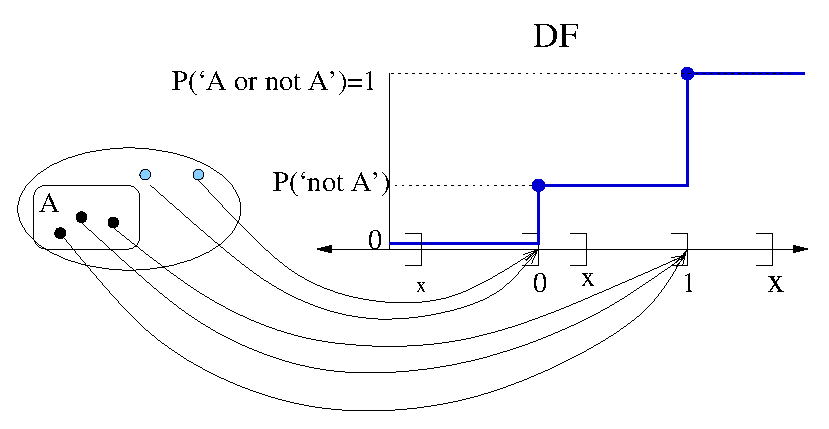
\includegraphics{figures/RVIndic}}
\end{figure}
\begin{classwork}[Indicator function is a random variable]
Let us convince ourselves that $\BB{1}_A$ is really a RV.  For $\BB{1}_A$ to be a RV, we need to verify that 
for any real number $x \in \Rz$, the inverse image $\BB{1}_A^{[-1]}( \ (- \infty, x] \ )$ is an event, ie :
\[
\BB{1}_A^{[-1]}( \ (- \infty, x] \ ) := \{\omega: \BB{1}_A(\omega) \leq x\} \in \C{F} \ .
\] 
All we can assume about the collection of events $\C{F}$ is that it contains the event $A$ and that it is a sigma algebra.  A careful look at the \hyperref[F:RVIndic]{Figure \ref*{F:RVIndic}} yields:
\begin{equation}
\BB{1}_A^{[-1]}( \ (- \infty, x] \ ) := \{\omega: \BB{1}_A(\omega) \leq x\} =
\begin{cases}
\emptyset & \text{if} \quad x < 0 \notag \\
A^c       & \text{if} \quad 0 \leq x < 1 \notag \\
A \cup A^c  = \Omega   & \text{if} \quad 1 \leq x  \notag 
\end{cases}
\end{equation}
Thus, $\BB{1}_A^{[-1]}( \ (- \infty, x] \ )$ is one of the following three sets that belong to $\C{F}$; (1) $\emptyset$, (2) $A^c$ and (3) $\Omega$ depending on the value taken by $x$ relative to the interval $[0,1]$.  We have proved that $\BB{1}_A$ is indeed a RV.
\end{classwork}
Some useful properties of the Indicator Function are:
\[
\BB{1}_{A^c} = 1 - \BB{1}_A, \qquad \BB{1}_{A \cap B} = \BB{1}_A \BB{1}_B, \qquad \BB{1}_{A \cup B} = \BB{1}_A + \BB{1}_B - \BB{1}_A \BB{1}_B
\]
We slightly abuse notation when $A$ is a single element set by ignoring the curly braces.
\begin{figure}[htpb]
\caption{A RV $X$ from a sample space $\Omega$ with $8$ elements to $\Rz$ and its DF $F$ \label{F:RVABC}}
\centering   \makebox{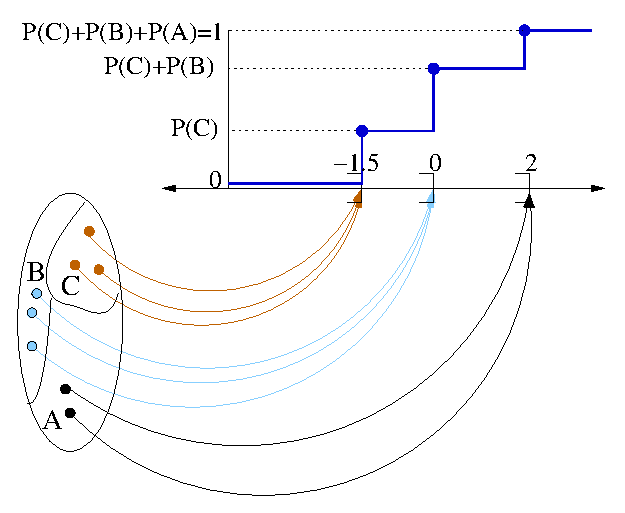
\includegraphics{figures/RV}}
\end{figure}
\begin{classwork}[A random variable with three values and eight sample points]
Consider the RV $X$ of \hyperref[F:RVABC]{Figure \ref*{F:RVABC}}.  Let the events $A = \{\omega_1, \omega_2\}$, $B = \{\omega_3, \omega_4, \omega_5\}$ and $C = \{\omega_6, \omega_7,\omega_8 \}$.  Define the RV $X$ formally.  What sets should $\C{F}$ minimally include?  What do you need to do to make sure that $\C{F}$ is a sigma algebra?
\vspace{4cm}
\end{classwork}

\section{An Elementary Discrete Random Variable}\label{S:ElemDiscRV}

When a RV takes at most countably many values from a discrete set $\Dz \subset \Rz$, we call it a {\bf discrete} RV.  Often, $\Dz$ is the set of integers $\Zz$.
\begin{definition}[probability mass function (PMF)]
Let $X$ be a discrete RV over a probability triple $(\Omega, \C{F},P)$.  We define the {\bf probability mass function} (PMF) $f$ of $X$ to be the function $f : \Dz \rightarrow [0,1]$ defined as follows:
\[
f(x) := \p(X=x) = \p( \ \{\omega: X(\omega) = x\} \ ), \qquad \text{where $x \in \Dz$.} 
\]
\end{definition}
The DF $F$ and PMF $f$ for a discrete RV $X$ satisfy the following:
\begin{enumerate}
\item  For any $x \in \Rz$,
\[
\p(X \leq x) = F(x) = \sum_{\Dz \ni y \leq x} f(y) := 
\sum_{y \ \in \  \Dz \cap (-\infty, x] } f(y) \ .
\]
\item For any $a,b \in \Dz$ with $a<b$,
\[
\p(a < X \leq b) = F(b) - F(a) = \sum_{y \ \in \  \Dz \cap (a, b] } f(y) \ .
\]
In particular, when $\Dz=\Zz$ and $a=b-1$,
\[
\p(b-1 < X \leq b) = F(b) - F(b-1) = f(b) = \p( \ \{ \omega : X(\omega) = b\} \ ) \ .
\]
\item And of course
\[
% \lim_{x \rightarrow \infty} F_X(x) = 1
\sum_{x \in \Dz} f(x) = 1
\]
\end{enumerate}

The Indicator Function $\BB{1}_A$ of the event that `$A$ occurs' for the $\theta$-specific experiment $\E{E}$ over some probability triple $(\Omega,\C{F},\p_{\theta})$, with $A \in \C{F}$, is the $\bernoulli(\theta)$ RV.  The parameter $\theta$ denotes the probability that `$A$ occurs' (see \hyperref[F:RVt1T]{Figure \ref*{F:RVt1T}} when $A$ is the event that `{\tt H} occurs').  This is our first example of a discrete RV.

\begin{model}[$\bernoulli(\theta)$]
Given a parameter $\theta \in [0,1]$, the probability mass function (PMF) for the $\bernoulli(\theta)$ RV $X$ is:
\begin{equation}\label{E:Bernoullipdf}
f(x;\theta)= \theta^x (1-\theta)^{1-x} \BB{1}_{\{0,1\}}(x) =
\begin{cases}
\theta & \text{if $x=1$,}\\
1-\theta & \text{if $x=0$,}\\
0 & \text{otherwise}
\end{cases}
\end{equation}
and its DF is:
\begin{equation}
F(x;\theta) =
\begin{cases}
1 & \text{if $1 \leq x$,}\\
1-\theta & \text{if $0 \leq x < 1$,}\\
0 & \text{otherwise}
\end{cases}
\end{equation}
We emphasise the dependence of the probabilities on the parameter $\theta$ by specifying it following the semicolon in the argument for $f$ and $F$ and by subscripting the probabilities, i.e.~$\p_{\theta}(X=1)=\theta$ and $\p_{\theta}(X=0)=1-\theta$.
\end{model}
\begin{figure}[htpb]
\caption{The Indicator Function $\BB{1}_{ \ {\tt H} \ }$ of the event `Heads occurs', for the experiment `Toss 1 times,' $\E{E}_{\theta}^{1}$, as the RV $X$ from the sample space $\Omega = \{ {\tt H}, {\tt T}\}$ to $\Rz$ and its DF $F$.  The probability that `Heads occurs' and that `Tails occurs' are $f(1;\theta)=\p_{\theta}(X=1) = \p_{\theta}({\tt H})=\theta$ and $f(0;\theta)=\p_{\theta}(X=0)=\p_{\theta}({\tt T})=1-\theta$, respectively.\label{F:RVt1T}}
\centering   \makebox{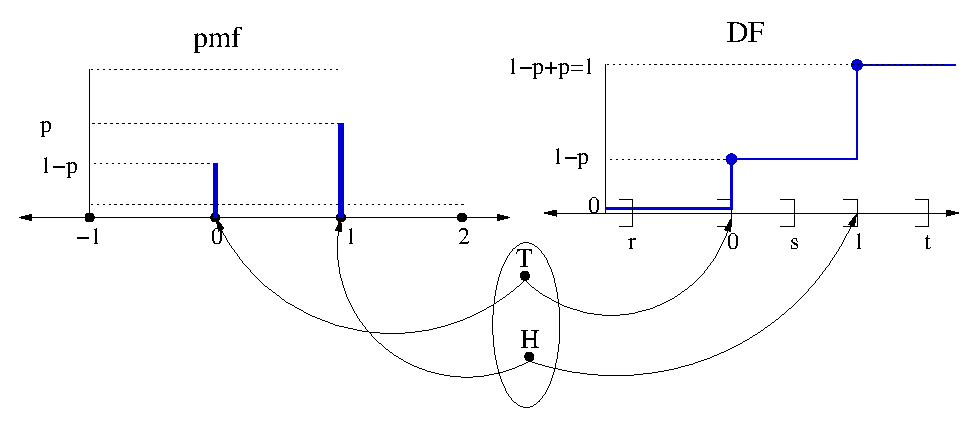
\includegraphics[width=6.5in]{figures/RVToss1}}
\end{figure}

\section{An Elementary Continuous Random Variable}\label{S:ElemContRV}

When a RV takes values in the continuum we call it a {\bf continuous} RV.  An example of such a RV is the vertical position (in micro meters) since the original release of a pollen grain on water.  Another example of a continuous RV is the volume of water (in cubic meters) that fell on the southern Alps last year.  
\begin{definition}[probability density function (PDF)]
A RV $X$ is said to be `continuous' if there exists a piecewise-continuous function $f$, called the probability density function (PDF) of $X$, such that for any $a, b \in \Rz$ with $a < b$,
\[
\p(a < X \leq b) = F(b)-F(a) = \int_a^b f(x) \ dx \ .
\]
\end{definition}
The following hold for a continuous RV $X$ with PDF $f$:
\begin{enumerate}
\item For any $x \in \Rz$, $\p(X=x)=0$.
\item Consequentially, for any $a,b \in \Rz$ with $a \leq b$,
\[
\p(a < X < b ) = \p(a < X \leq b) = \p(a \leq X \leq b) = \p(a \leq X < b) \ .
\]
\item By the fundamental theorem of calculus, except possibly at finitely many points (where the continuous pieces come together in the piecewise-continuous $f$):
\[
f(x) = \frac{d}{dx} F(x)
\]
\item And of course $f$ must satisfy:
\[
\int_{-\infty}^{\infty} f(x) \ dx = \p(-\infty < X < \infty) = 1 \ .
\] 
\end{enumerate}

An elementary and fundamental example of a continuous RV is the $\uniform(0,1)$ RV of \hyperref[M:Uniform01]{Model \ref*{M:Uniform01}}.  It forms the foundation for random variate generation and simulation.  In fact, it is appropriate to call this the fundamental model since every other experiment can be obtained from this one.

\begin{model}[The Fundamental Model]\label{M:Uniform01}
The probability density function (PDF) of the fundamental model or the $\uniform(0,1)$ RV is
\begin{equation}\label{E:Uniform01pdf}
f(x) = \BB{1}_{[0,1]}(x) = 
\begin{cases}
1 & \text{if $0 \leq x \leq 1$,}\\
0 & \text{otherwise}
\end{cases}
\end{equation}
and its distribution function (DF) or cumulative distribution function (CDF) is:
\begin{equation}\label{E:Uniform01DF}
F(x) := \int_{- \infty}^x f(y) \ dy =
\begin{cases}
0 & \text{if $x < 0$,} \\
x & \text{if $0 \leq x \leq 1$,}\\
1 & \text{if $x > 1$} 
\end{cases}
\end{equation}
Note that the DF is the identity map in $[0,1]$.  The PDF and DF are depicted in \hyperref[F:unif01]{Figure~\ref*{F:unif01}}.
\begin{figure}[htpb]
\caption{A plot of the PDF and DF or CDF of the $\uniform(0,1)$ continuous RV $X$.\label{F:unif01}}
\centering   \makebox{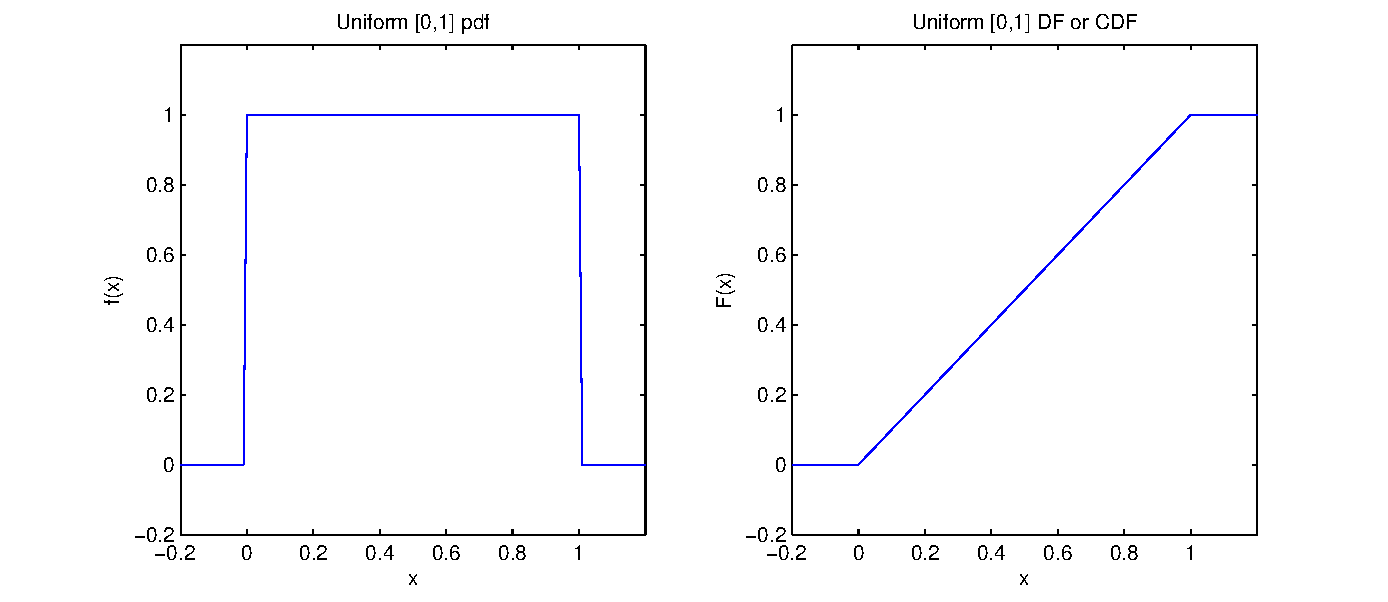
\includegraphics[width=6.5in]{figures/Unif01pdfcdf}}
\end{figure}
\end{model}

\remove{
\begin{labwork}[PDF of $\uniform(0,1)$ RV]\label{LW:Unif01Pdf}
Let us encode the PDF of $\uniform(0,1)$ as an M-file in {\sc Matlab}.  Notice that the PDF function assigns $1$ to every value of $x \in [0,1]$ and $0$ to every value of $x \notin [0,1]$.  So, the problem mostly boils down to finding the entries inside and outside the range.  We can use {\sc Matlab}'s built-in {\tt find} function for this purpose.  We give an example to illustrate the syntax of {\tt find}.
\begin{VrbM}
>> Xs=[0.2511    1.6160    0.4733    -5.3517    0.8308    0.5853    2.5497] % an array Xs with real values 
Xs =    0.2511    1.6160    0.4733   -5.3517    0.8308    0.5853    2.5497
\end{VrbM}
We can obtain the indices of {\tt Xs} whose values are $\geq 0$, i.e.~$\{i: {\tt Xs}(i) \geq 0 \}$ and the indices of {\tt Xs} whose values are $\leq 1$, i.e.~$\{i: {\tt Xs}(i) \leq 1 \}$ as follows:
\begin{VrbM}
>> find(Xs >= 0)
ans =     1     2     3     5     6     7
>> find(Xs <= 1)
ans =     1     3     4     5     6
\end{VrbM}
The intersection of the two sets of indices, i.e.~$\{i: {\tt Xs}(i) \geq 0 \ \text{ and } \  {\tt Xs}(i) \leq 1 \} = \{i: 0 \leq {\tt Xs}(i) \leq 1 \}$ can be obtained by {\tt \&}, the Boolean and, as follows:
\begin{VrbM}
>> find(Xs >= 0 & Xs <= 1)
ans =     1     3     5     6
\end{VrbM}
Finally, we know which indices of the {\tt Xs} array should have the PDF value of $1$.  The remaining indices of {\tt Xs} should therefore have the PDF value of $0$.  Let us declare an array called {\tt Pdf} for the PDF values corresponding to the {\tt Xs}.  We can initialise this array with zeros using the {\tt zeros} function and make it of the same size as {\tt Xs} as follows:
\begin{VrbM}
>> size(Xs)
ans =     1     7
>> Pdf = zeros(1,7)
Pdf =     0     0     0     0     0     0     0
\end{VrbM}
Now, we can set the indices $1,3,5,6$ (returned by {\tt find(Xs >= 0 \& Xs <= 1)}) of {\tt Pdf} array to 1.
\begin{VrbM}
>> Pdf([1     3     5     6])=1
Pdf =     1     0     1     0     1     1     0
\end{VrbM}
We can modularise this process for an arbitrary input array {\tt x} via a function in the following M-file.
\VrbMf[label=Unif01Pdf.m]{scripts/Unif01Pdf.m} 
Let us call the function we wrote called {\tt Unif01Pdf} next.
\begin{VrbM}
>> help Unif01Pdf
  Unif01Pdf(x) returns the PDF of Uniform(0,1) RV X
  the input x can be an array
>> Xs
Xs =    0.2511    1.6160    0.4733   -5.3517    0.8308    0.5853    2.5497
>> Unif01Pdf(Xs)
ans =     1     0     1     0     1     1     0
\end{VrbM}
\end{labwork}

\begin{labwork}[CDF of $\uniform(0,1)$ RV]\label{LW:Unif01Cdf}
Understand each step in the function {\tt Unif01Cdf}:
\VrbMf[label=Unif01Cdf.m]{scripts/Unif01Cdf.m} 
When we type in {\tt help Unif01Cdf}, {\tt Xs} and {\tt Unif01Cdf(Xs)} we can confirm that the {\tt Unif01Cdf} function is correctly reporting the CDF values of the input array {\tt Xs}.
\begin{VrbM}
>> help Unif01Cdf
  Unif01Cdf(x) returns the CDF of Uniform(0,1) RV X
  the input x can be an array 
>> Xs
Xs =    0.2511    1.6160    0.4733   -5.3517    0.8308    0.5853    2.5497
>> Unif01Cdf(Xs)
ans =    0.2511    1.0000    0.4733         0    0.8308    0.5853    1.0000
\end{VrbM}
\end{labwork}

\begin{labwork}[Plot of the PDF and the CDF for the $\uniform(0,1)$ RV]\label{LW:PlotUnif01PdfCdf}
Generate the plot of the PDF and the CDF for the $\uniform(0,1)$ RV $X$ by following the commands below.  Go through every step and understand each command when you reproduce the plot.
\VrbMf[label=plotunif.m]{scripts/plotunif.m} 
The plot was saved as an encapsulated postscript file from the File menu of the Figure window and is displayed in \hyperref[F:unif01]{Figure~\ref*{F:unif01}}.
 \end{labwork}
}

{\bf **tossing a fair coin infinitely often and the fundamental model}

%TODO\input{figures/UnifsInUnif.tex}

--- The fundamental model is equivalent to infinite tosses of a fair coin (see using binary expansion of any $x \in (0,1)$)

--- The fundamental model has infinitely many copies of itself within it!


{\bf **universality of the fundamental model}

--- one can obtain any other random object from the fundamental model!

\section{Transformations of random variables}\label{S:TransformationsOFRvs}

Suppose we know the distribution of a random variable $X$.  How do we find the distribution of a transformation of $X$, say $g(X)$?
Before we answer this question let us ask a motivational question.  Why are we interested in functions of random variables?

\begin{example}
Consider a simple financial example where an individual sells $X$ items per day, the profit per item is $\$ 5$ and the overhead costs are $\$ 500$ per day.  The original random variable is $X$, but the random variable $Y$ which gives the daily profit is of more interest, where
\[
Y = 5X - 500 \enspace . 
\]
\end{example}

\begin{example}
In a cell-phone system a mobile signal may have a signal-to-noise-ratio of $X$, but engineers prefer to express such ratios in decibels, i.e.,
\[
Y = 10 \log_{10}(X) \enspace .
\]
\end{example}

Hence in a great many situations we are more interested in functions of random variables. 
Let us return to our original question of determining the distribution of a transformation or function of $X$.  
First note that this transformation of $X$ is itself another random variable, say $Y = g(X)$, 
where $g$ is a function from a subset $\mathbb{X}$ of $\mathbb{R}$ to a subset $\mathbb{Y}$ of $\mathbb{R}$, 
i.e., $g: \mathbb{X} \to \mathbb{Y}$, $\mathbb{X} \subset \mathbb{R}$ and $\mathbb{Y} \subset \mathbb{R}$.

The {\bf inverse image} of a set $A$ is the set of all real numbers in $\mathbb{X}$ whose image is in $A$, i.e.,
\[
g^{[-1]}(A) = \{x \in \mathbb{X} : g(x) \in A \} \enspace .
\] 
In other words,
\[
x \in g^{[-1]}(A) \ \text{if and only if} \ g(x) \in A \enspace .
\]
For example,
\begin{itemize}
\item if $g(x)=2x$ then $g^{[-1]}([4,6])=[2,3]$
\item if $g(x)=2x+1$ then $g^{[-1]}([5,7])=[2,3]$
\item if $g(x)=x^3$ then $g^{[-1]}([1,8])=[1,2]$
\item if $g(x)=x^2$ then $g^{[-1]}([1,4])=[-2,-1] \cup [1,2]$
\item if $g(x)=\sin(x)$ then $g^{[-1]}([-1,1])=\mathbb{R}$
\item if ... %Raaz add other examples of the transformations done in the sequel here
\end{itemize}
For the singleton set $A = \{y\}$, we write $g^{[-1]}(y)$ instead of $g^{[-1]}(\{y\})$.  
For example,
\begin{itemize}
\item if $g(x)=2x$ then $g^{[-1]}(4)=\{2\}$
\item if $g(x)=2x+1$ then $g^{[-1]}(7)=\{3\}$
\item if $g(x)=x^3$ then $g^{[-1]}(8)=\{2\}$
\item if $g(x)=x^2$ then $g^{[-1]}(4)=\{-2,2\}$
\item if $g(x)=\sin(x)$ then $g^{[-1]}(0)=\{k \pi: k \in \mathbb{Z}\} = \{\ldots, -3 \pi, -2 \pi, -\pi,0,\pi, 2\pi,3\pi, \ldots\}$
\item if ... %Raaz add other examples of the transformations done in the sequel here
\end{itemize}
If $g:\mathbb{X}\to\mathbb{Y}$ is one-to-one (injective) and onto (surjective), then the inverse image of a singleton set is itself a singleton set.  
Thus, the inverse image of such a function $g$ becomes itself a function and is called the {\bf inverse function}.
One can find the inverse function, if it exists by the following steps:
\begin{itemize}
\item[{\sf Step 1;}] write $y=g(x)$
\item[{\sf Step 2;}] solve for $x$ in terms of $y$
\item[{\sf Step 3;}] set $g^{-1}(y)$ to be this solution
\end{itemize}
We write $g^{-1}$ whenever the inverse image $g^{[-1]}$ exists as an inverse function of $g$.  
Thus, the inverse function $g^{-1}$ is a specific type of inverse image $g^{[-1]}$.  
For example,
\begin{itemize}
\item if $g(x)=2x$ then $g:\mathbb{R} \to \mathbb{R}$ is injective and surjective and therefore its inverse function is:\\
{\sf Step 1;} $y=2x$, {\sf Step 2;} $x=\frac{y}{2}$, {\sf Step 3;} $g^{-1}(y)=\frac{y}{2}$
\item if $g(x)=2x+1$ then $g:\mathbb{R} \to \mathbb{R}$ is injective and surjective and therefore its inverse function is:\\
{\sf Step 1;} $y=2x+1$, {\sf Step 2;} $x=\frac{y-1}{2}$, {\sf Step 3;} $g^{-1}(y)=\frac{y-1}{2}$
\item if $g(x)=x^3$ then $g:\mathbb{R} \to \mathbb{R}$ is injective and surjective and therefore its inverse function is:\\
{\sf Step 1;} $y=x^3$, {\sf Step 2;} $x={y}^{\frac{1}{3}}$, {\sf Step 3;} $g^{-1}(y)={y}^{\frac{1}{3}}$
\end{itemize}
However, you need to be careful by limiting the domain to obtain the inverse function for the following examples:
\begin{itemize}
\item if $g(x)=x^2$ and domain of $g$ is $[0,+\infty)$ then its inverse function is $g^{-1}(y)=\sqrt{y}$, 
i.e., if $g(x)=x^2 : [0,+\infty) \to [0,+\infty)$ then the inverse image $g^{[-1]}(y)$ for $y \in [0,+\infty)$ is given by the inverse function $g^{-1}(y)=\sqrt{y} : [0,+\infty) \to [0,+\infty)$.
\item if $g(x)=x^2$ and domain of $g$ is $(-\infty,0]$ then its inverse function is $g^{-1}(y)=-\sqrt{y}$, 
i.e., if $g(x)=x^2 : (-\infty,0] \to [0,+\infty)$ then the inverse image $g^{[-1]}(y)$ for $y \in [0,+\infty)$ is given by the inverse function $g^{-1}(y)=-\sqrt{y} : [0,+\infty) \to (-\infty,0]$.
\item if $g(x)=\sin(x)$ and domain of $g$ is $[0,\frac{\pi}{2}]$ then its inverse function $g^{-1}(y)=\arcsin(y)$, i.e., if $g(x)=\sin(x) : [0,\frac{\pi}{2}] \to [0,1]$ then the inverse image $g^{[-1]}(y)$ for $y \in [0,1]$ is given by the inverse function $g^{-1}(y)=\arcsin(y) : [0,1] \to [0, \frac{\pi}{2}]$.
\item if $g(x)=\sin(x)$ and domain of $g$ is $[-\frac{\pi}{2},\frac{\pi}{2}]$ then its inverse function $g^{-1}(y)=\arcsin(y)$, i.e., if $g(x)=\sin(x) : [-\frac{\pi}{2},\frac{\pi}{2}] \to [-1,1]$ then the inverse image $g^{[-1]}(y)$ for $y \in [-1,1]$ is given by the inverse function $g^{-1}(y)=\arcsin(y) : [-1,1] \to [-\frac{\pi}{2},\frac{\pi}{2}]$.
\item if ... %Raaz add other examples of the transformations done in the sequel here
\end{itemize}
  
Now, let us return to our question of determining the distribution of the transformation $g(X)$.  To answer this question we must first observe that the inverse image $g^{[-1]}$ satisfies the following properties:
\begin{itemize}
\item $g^{[-1]}(\mathbb{Y}) = \mathbb{X}$
\item For any set $A$, $g^{[-1]}(A^c) = \left(g^{[-1]}(A)\right)^c$
\item For any collection of sets $\{A_1,A_2,\ldots\}$,
\[
g^{[-1]}\left( A_1 \cup A_2 \cup \cdots \right) = g^{[-1]}(A_1) \cup g^{[-1]}(A_2) \cup \cdots \enspace.
\]
\end{itemize}
Consequentially, 
\begin{equation}\label{E:ProbOfgOfX}
\boxed{P \left( g(X) \in A \right) = P \left(X \in g^{[-1]}(A) \right)}
\end{equation} 
satisfies the axioms of probability and gives the desired probability of the event $A$ from the transformation $Y=g(X)$ in terms of the probability of the event given by the inverse image of $A$ underpinned by the random variable $X$.  
It is crucial to understand this from the sample space $\Omega$ of the underlying experiment in the sense that Equation~\eqref{E:ProbOfgOfX} is just short-hand for its actual meaning:
\[
P \left( \{\omega \in \Omega: g(X(\omega)) \in A\} \right) 
= P \left( \left\{ \omega \in \Omega: X(\omega) \in g^{[-1]}(A) \right\} \right) \enspace .
\]
Because we have more than one random variable to consider, namely, $X$ and its transformation $Y=g(X)$ we will subscript the probability density or mass function and the distribution function by the random varaible itself.  For example we denote the distribution function of $X$ by $F_X(x)$ and that of $Y$ by $F_Y(y)$.

\subsection{Transformation of discrete random variables}
For a discrete random variable $X$ with probability mass function $f_X$ we can obtain the probability mass function $f_Y$ of $Y=g(X)$ using Equation~\eqref{E:ProbOfgOfX} as follows:
\begin{eqnarray*}
f_Y(y) 
&=& P(Y =y) = P(Y \in \{y\}) \\
&=& P \left( g(X) \in \{y\} \right) = P \left(X \in g^{[-1]}(\{y\}) \right)\\
&=& P \left(X \in g^{[-1]}(y) \right) = \sum_{x \in g^{[-1]}(y)} f_X(x) = \sum_{x \in \{x: g(x)=y\}} f_X(x) \enspace .
\end{eqnarray*}
This gives the formula:
\begin{equation}\label{E:PMFOfgOfX}
\boxed{
f_Y(y) = P(Y =y) = \sum_{x \in g^{[-1]}(y)} f_X(x) = \sum_{x \in \{x: g(x)=y\}} f_X(x) \enspace .
}
\end{equation}

\begin{example}\label{EXMP:Discrete1to1TransYis2X}
Let $X$ be the discrete random variable with probability mass function $f_X$ as tabulated below:\\
\begin{center}
\begin{tabular}{r|rrr}
$x$ & -1 & 0 & 1\\ \hline
 &  &  & \\ 
$f_X(x)=P(X=x)$ & $\frac{1}{4}$ & $\frac{1}{2}$ & $\frac{1}{4}$
\end{tabular}
\end{center}
If $Y=2X$ then the transformation $g(X)=2X$ has inverse image $g^{[-1]}(y)=\{y/2\}$.  
Then, by Equation~\eqref{E:PMFOfgOfX} the probability mass function of $Y$ is expressed in terms of the known probabilities of $X$ as:\\ 
$$f_Y(y)=P(Y=y)= \sum_{x \in g^{[-1]}(y)} f_X(x)  = \sum_{x \in \{y/2\}} f_X(x) = f_X(y/2) \enspace ,$$
and tabulated below:\\
\begin{center}
\begin{tabular}{r|rrr}
$y$ & -2 & 0 & 2\\ \hline
 &  &  & \\ 
$f_Y(y)$ & $\frac{1}{4}$ & $\frac{1}{2}$ & $\frac{1}{4}$
\end{tabular}
\end{center}
\end{example}

\begin{example}\label{EXMP:Discrete1to1TransYis2Xplus1}
If $X$ is the random variable in the previous Example then what is the probability mass function of $Y=2X+1$?
Once again,
$$f_Y(y)=P(Y=y)= \sum_{x \in g^{[-1]}(y)} f_X(x)  = \sum_{x \in \{(y-1)/2\}} f_X(x) = f_X((y-1)/2) \enspace ,$$
and tabulated below:\\
\begin{center}
\begin{tabular}{r|rrr}
$y$ & -1 & 1 & 3\\ \hline
 &  &  & \\ 
$f_Y(y)$ & $\frac{1}{4}$ & $\frac{1}{2}$ & $\frac{1}{4}$
\end{tabular}
\end{center}
\end{example}

In fact, obtaining the probability of a one-to-one transformation of a discrete random variable as in Examples~\ref{EXMP:Discrete1to1TransYis2X} and \ref{EXMP:Discrete1to1TransYis2Xplus1} is merely a matter of looking up the probability at the image of the inverse function.  This is because there is only one term in the sum that appears in Equation~\eqref{E:PMFOfgOfX}.  When the transformation is not one-to-one the number of terms in the sum can be more than one as shown in the next Example.

\begin{example}
Reconsider the random variable $X$ of the last two Examples and let $Y=X^2$.  
Recall that $g(x)=x^2$ does not have an inverse function unless the domain is restricted to the positive or the negative parts of the real line.  
Since our random variable $X$ takes values on both sides of the real line, namely $\{-1,0,1\}$, let us note that the transformation $g(X)=X^2$ is no longer a one-to-one function.  
Then, by Equation~\eqref{E:PMFOfgOfX} the probability mass function of $Y$ is expressed in terms of the known probabilities of $X$ as:\\ 
\[
f_Y(y)=P(Y=y)= \sum_{x \in g^{[-1]}(y)} f_X(x)  = \sum_{\{x:g(x)=y\}} f_X(x) = \sum_{\{x:x^2=y\}} f_X(x) \enspace ,
\]
computed for each $y \in \{0,1\}$ as follows:
\begin{eqnarray*}
f_Y(0) &=& \sum_{\{x:x^2=0\}} f_X(x) = f_X(0)=\frac{1}{2} \enspace ,\\
f_Y(1) &=& \sum_{\{x:x^2=1\}} f_X(x) = f_X(-1)+f_X(1)=\frac{1}{4}+\frac{1}{4}=\frac{1}{2} \enspace ,
\end{eqnarray*}
and finally tabulated below:\\
\begin{center}
\begin{tabular}{r|ccc}
$y$ & 0 & & 1\\ \hline
 &  &  & \\ 
$f_Y(y)$ & $\frac{1}{2}$ & \quad & $\frac{1}{2}$
\end{tabular}\enspace .
\end{center}
\end{example}

\subsection{Transformation of continuous random variables}
Suppose we know $F_X$ and/or $f_X$ of a continuous random variable $X$.  
Let $Y=g(X)$ be a transformation of $X$.  
Our objective is to obtain $F_Y$ and/or $f_Y$ of $Y$ from $F_X$ and/or $f_X$.  
%We will look at two techniques in Sections~\ref{S:DirectMethod} and \ref{S:f_YDirectlyFromf_X} to achieve our objective.

\subsubsection{One-to-one transformations}\label{S:f_YDirectlyFromf_X}
The easiest case for transformations of continuous random variables is when $g$ is {\bf one-to-one and monotone}.  
\begin{itemize}
\item{
First, let us consider the case when $g$ is {\bf monotone and increasing} on the range of the random variable $X$.  
In this case $g^{-1}$ is also an increasing function and we can obtain the distribution function of $Y=g(X)$ in terms of the distribution function of $X$ as   
\[
F_Y(y) =P \left(Y \leq y \right)=P \left(g(X) \leq y \right) = P \left(X \leq g^{-1}(y) \right) = F_X(g^{-1}(y)) \enspace .
\]
Now, let us use a form of chainrule to compute the density of $Y$ as follows:
\[
f_Y(y) 
= \frac{d}{dy} F_Y(y)
= \frac{d}{dy} F_X \left(g^{-1}(y) \right)
= f_X \left( g^{-1}(y) \right) \frac{d}{dy} \left(g^{-1}(y) \right) \enspace . 
\]
}
\item{
Second, let us consider the case when $g$ is {\bf monotone and decreasing} on the range of the random variable $X$.  
In this case $g^{-1}$ is also a decreasing function and we can obtain the distribution function of $Y=g(X)$ in terms of the distribution function of $X$ as   
\[
F_Y(y) =P \left(Y \leq y \right)=P \left(g(X) \leq y \right) = P \left(X \geq g^{-1}(y) \right) = 1- F_X(g^{-1}(y)) \enspace ,
\]
and the density of $Y$ as 
\[
f_Y(y) 
= \frac{d}{dy} F_Y(y)
= \frac{d}{dy} \left(1-F_X \left(g^{-1}(y) \right) \right)
= -f_X \left( g^{-1}(y) \right) \frac{d}{dy} \left(g^{-1}(y) \right) \enspace . 
\]
For a monotonic and decreasing $g$, its inverse function $g^{-1}$ is also decreasing and consequently the density $f_Y$ is indeed positive because $\frac{d}{dy} \left(g^{-1}(y) \right)$ is negative.  
}
\end{itemize}
We can combine the above two cases and obtain the following 
{\bf change of variable formula} for the probability density of $Y=g(X)$ when $g$ is one-to-one and monotone on the range of $X$.
\begin{equation}\label{E:f_YFromf_X_Under_one-to-one-g}
\boxed{
f_Y(y) = f_X \left( g^{-1}(y) \right) \left\vert \frac{d}{dy} g^{-1}(y) \right\vert \enspace .}
\end{equation}

The steps involved in finding the density of $Y=g(X)$ for a one-to-one and monotone $g$ are:
\begin{enumerate}
\item Write $y=g(x)$ for $x$ in range of $x$ and check that $g(x)$ is monotone over the required range to apply the change of variable formula. 
\item Write $x=g^{-1}(y)$ for $y$ in range of $y$.
\item Obtain $\left\vert \frac{d}{dy} g^{-1}(y) \right\vert$ for $y$ in range of $y$.
\item Finally, from Equation~\eqref{E:f_YFromf_X_Under_one-to-one-g} get $f_Y(y) = f_X \left( g^{-1}(y) \right) \left\vert \frac{d}{dy} g^{-1}(y) \right\vert$ for $y$ in range of $y$. 
\end{enumerate}

Let us use these four steps to obtain the density of monotone transformations of continuous random variables.

\begin{example}
Let $X$ be $\uniform(0,1)$ random variable and let $Y=g(X)=1-X$.  
We are interested in the density of the tranformed random variable $Y$. Let us follow the four steps and use the change of variable formula to obtain $f_Y$ from $f_X$ and $g$.
\begin{enumerate}
\item $y=g(x)=1-x$ is a monotone decreasing function over $0 \leq x \leq 1$, the range of $X$.  
So, we can apply the change of variable formula. 
\item $x=g^{-1}(y)=1-y$ is a monotone decreasing function over $1-0 \geq 1-x \geq 1-1$, i.e., $0 \leq y \leq 1$.  
\item For $0 \leq y \leq 1$,
\[
 \left\vert \frac{d}{dy} g^{-1}(y) \right\vert 
= \left\vert \frac{d}{dy} \left( 1-y \right) \right\vert 
= \left\vert -1 \right\vert = 1 \enspace .
\]
\item we can use Equation~\eqref{E:f_YFromf_X_Under_one-to-one-g} to find the density of $Y$ as follows:
\[
f_Y(y) = f_X \left( g^{-1}(y) \right) \left\vert \frac{d}{dy} g^{-1}(y) \right\vert 
= f_X \left( 1-y \right)  \, 1
= 1 \enspace ,
\]
for $0 \leq y \leq 1$
\end{enumerate}
Thus, we have shown that if $X$ is a $\uniform(0,1)$ random variable then $Y=1-X$ is also a $\uniform(0,1)$ random variable.
\end{example}

\begin{example}
Let $X$ be a $\uniform(0,1)$ random variable and let $Y=g(X)=-\log(X)$.  
We are interested in the density of the tranformed random variable $Y$.  
Once again, since $g$ is a one-to-one monotone function let us follow the four steps and use the change of variable formula to obtain $f_Y$ from $f_X$ and $g$.
\begin{enumerate}
\item $y=g(x)=-\log(x)$ is a monotone decreasing function over $0 < x < 1$, the range of $X$.  
So, we can apply the change of variable formula. 
\item $x=g^{-1}(y)=\exp(-y)$ is a monotone decreasing function over %$-\log(0) > -\log(x) > -\log(1)$, i.e., %Ben does not like -\log(0)=-\infty because -\log(0) is said to be undefined to these students -- raaz expected -\log(0) = \lim_{x \to 0^+} \log(x) = -\infty is reasonable to assume here.
$0 < y < \infty$.  
\item For $0 < y < \infty$,
\[
 \left\vert \frac{d}{dy} g^{-1}(y) \right\vert 
= \left\vert \frac{d}{dy} \left( \exp(-y) \right) \right\vert 
= \left\vert -\exp(-y) \right\vert = \exp(-y) \enspace .
\]
\item We can use Equation~\eqref{E:f_YFromf_X_Under_one-to-one-g} to find the density of $Y$ as follows:
\[
f_Y(y) = f_X \left( g^{-1}(y) \right) \left\vert \frac{d}{dy} g^{-1}(y) \right\vert 
= f_X \left( \exp(-y) \right)  \, \exp(-y)
= 1 \, \exp(-y) = \exp(-y) \enspace .
\]
Note that $0 < \exp(-y) < 1$ for $0 < y < \infty$.
\end{enumerate}
Thus, we have shown that if $X$ is a $\uniform(0,1)$ random variable then $Y=-\log(X)$ is an random variable with PDF $f_Y(y)=\BB{1}_{(0,\infty)}(y)\exp(-y)$. 
We can similarly show that for a parameter $\lambda>0$, if $X \sim \uniform(0,1)$ then $Y=-\lambda^{-1} \log(X)$ yields a probability model of RVs that are parameterized by $\lambda$ and extremely useful in applications. We introduce it next.
\end{example}

\begin{model}[$\exponential(\lambda)$]\label{M:exponential}
For a given $\lambda > 0$, an $\exponential(\lambda)$ RV has the following PDF $f$ and DF $F$:
\begin{eqnarray}\label{E:Exponentialpdfcdf}
f(x; \lambda) = \lambda e^{-\lambda x} \qquad &
F(x; \lambda)= 1-e^{-\lambda x}  \ .
\end{eqnarray}
This distribution is fundamental because of its property of {\bf memorylessness} and plays a fundamental role in continuous time
%Markov
processes as we will see later.
\end{model}

\remove{
We encode the PDF and DF of the $\exponential(\lambda)$ RV as \Matlab functions {\tt ExponentialPdf} and {\tt ExponentialCdf} and use them to produce \hyperref[F:plotPdfCdfExponentials]{Figure~\ref*{F:plotPdfCdfExponentials}} in \hyperref[Mf:ExponentialPdfCdf]{Labwork~\ref*{Mf:ExponentialPdfCdf}}.
}%end remove

\begin{figure}[htpb]
\caption{Density and distribution functions of $\exponential(\lambda)$ RVs, for $\lambda=1, 10, 10^{-1}$, in four different axes scales.\label{F:plotPdfCdfExponentials}}
\centering   \makebox{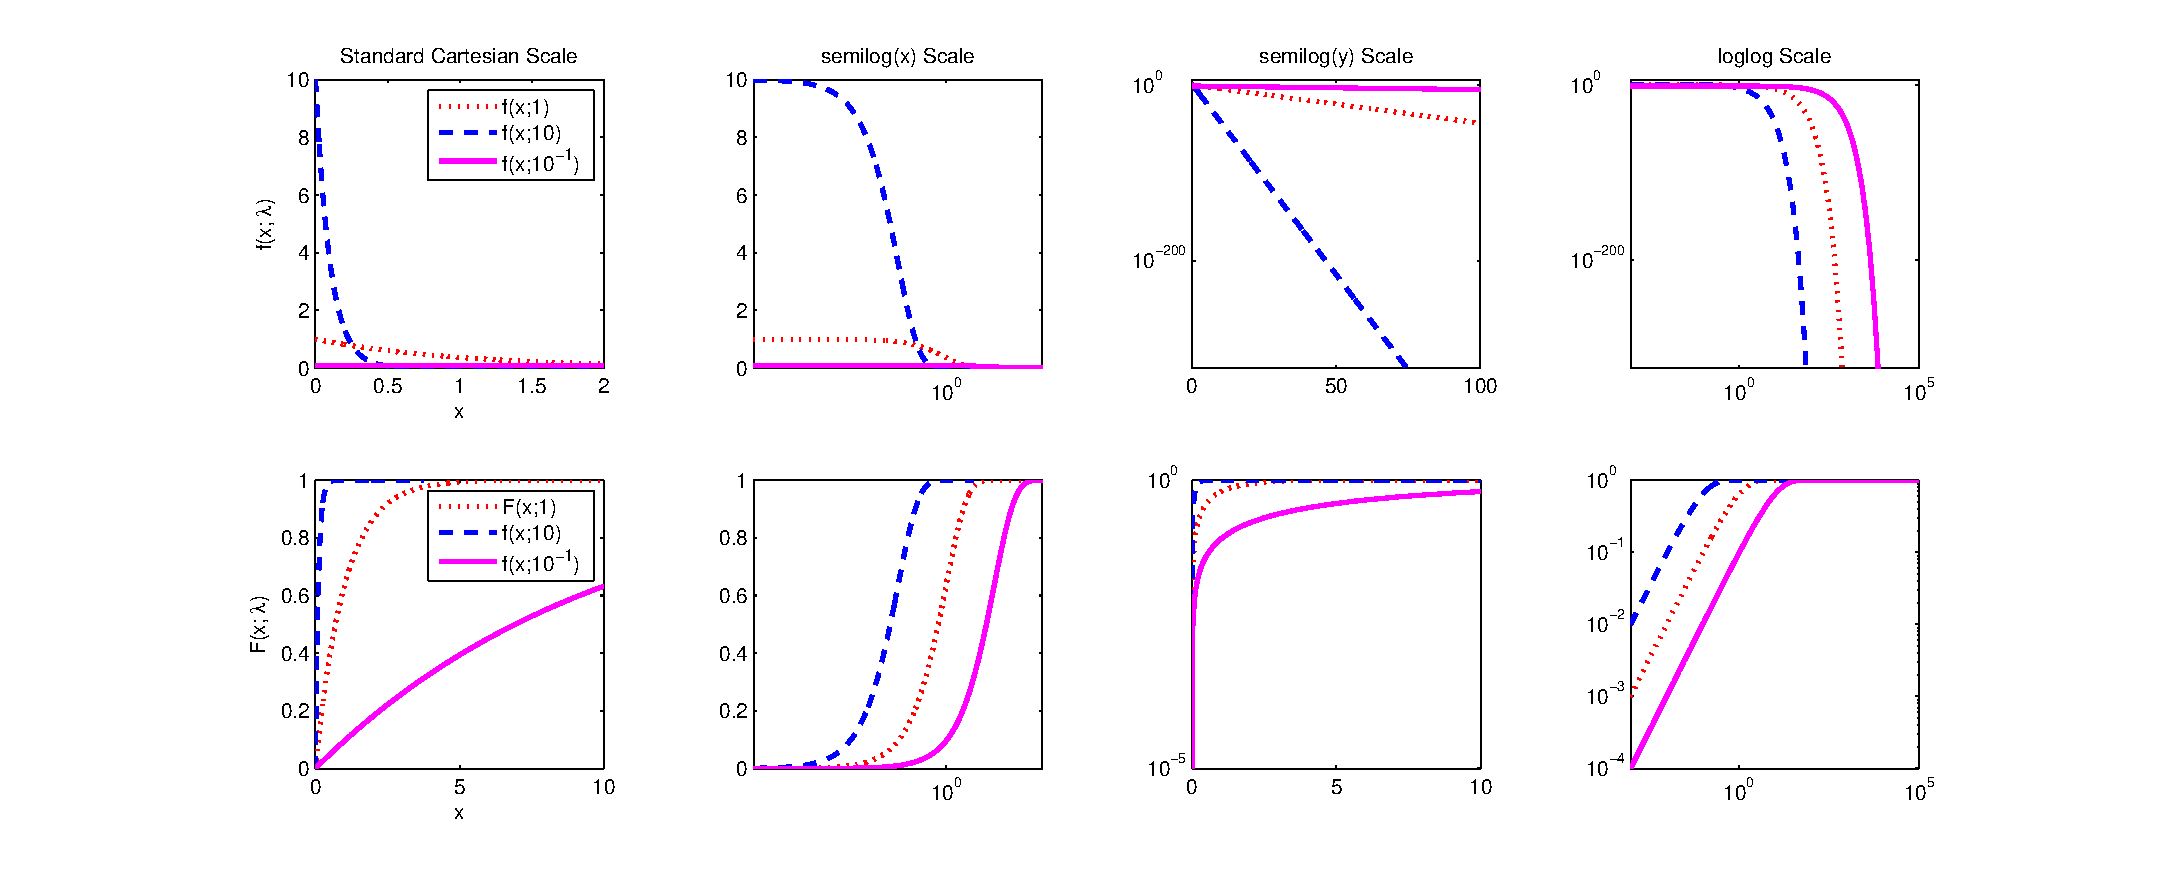
\includegraphics[width=6.5in]{figures/plotPdfCdfExponentials}}
\end{figure}


\subsubsection{Direct method}\label{S:DirectMethod}
If the transformation $g$ in $Y=g(X)$ is not necessarily one-to-one then special care is needed to obtain the distribution function or density of $Y$.  
For a continuous random variable $X$ with a known distribution function $F_X$ we can obtain the distribution function $F_Y$ of $Y=g(X)$ using Equation~\eqref{E:ProbOfgOfX} as follows:
\begin{eqnarray*}
F_Y(y)
&=& P \left(Y \leq y \right) = P \left(Y \in (-\infty, y] \right)\\
&=& P \left( g(X) \in (-\infty, y] \right) = P \left( X \in g^{[-1]}((-\infty, y]) \right) = P \left(X \in \{x: g(x) \in (-\infty,y]\}  \right) \enspace . %\\
\end{eqnarray*}
In words, the above equalities just mean that the probability that $Y \leq y$ is the probability that $X$ takes a value $x$ that satisfies $g(x) \leq y$.  
We can use this approach if it is reasonably easy to find the set $g^{[-1]}((-\infty,y]) = \{x: g(x) = (-\infty,y]\}$.% as done in Section~\ref{S:DirectMethod}.

\begin{example}
Let $X$ be any random variable with distribution function $F_X$.  Let $Y=g(X)=X^2$.  
Then we can find $F_Y$, the distribution function of $Y$ from $F_X$ as follows:
\begin{itemize}
\item {Since $Y=X^2 \geq 0$, if $y < 0$ then $F_Y(y) = P\left( X \in \{ x : x^2 < y\} \right) = P(X \in \emptyset) = 0$.}
\item {If $y \geq 0$ then
\begin{eqnarray*}
F_Y(y) = P \left(Y \leq y \right) 
&=& P \left( X^2 \leq y \right) \\
&=& P \left( -\sqrt{y} \leq X \leq \sqrt{y} \right) \\
&=& F_X(\sqrt{y}) - F_X(-\sqrt{y}) \enspace .
\end{eqnarray*}
}
\end{itemize}
By differentiation we get:
\begin{itemize}
\item {If $y<0$ then $f_Y(y)=\frac{d}{dy}(F_Y(y)) = \frac{d}{dy} 0 = 0$.}
\item {If $y \geq 0$ then
\begin{eqnarray*}
f_Y(y) 
= \frac{d}{dy}\left( F_Y(y) \right) 
&=& \frac{d}{dy}\left( F_X(\sqrt{y}) - F_X( - \sqrt{y}) \right)\\
&=& \frac{d}{dy}\left( F_X(\sqrt{y}) \right) - \frac{d}{dy}\left( F_X( - \sqrt{y}) \right)\\
&=& \frac{1}{2}y^{-\frac{1}{2}} f_X(\sqrt{y}) - \left( -\frac{1}{2}y^{-\frac{1}{2}} f_X( - \sqrt{y}) \right)\\
&=& \frac{1}{2 \sqrt{y}} \left( f_X(\sqrt{y}) + f_X( - \sqrt{y}) \right) \enspace .
\end{eqnarray*}
}
\end{itemize}
Therefore, the distribution function of $Y=X^2$ is:
\begin{equation}\label{E:F_YofX^2}
F_Y(y) = 
\begin{cases}
0 & \text{ if } y < 0 \\
F_X(\sqrt{y}) - F_X(-\sqrt{y}) & \text{ if } y \geq 0 \enspace .
\end{cases}
\end{equation}
and the probability density function of $Y=X^2$ is:
\begin{equation}\label{E:f_YofX^2}
f_Y(y) = 
\begin{cases}
0 & \text{ if } y < 0 \\
\frac{1}{2 \sqrt{y}} \left( f_X(\sqrt{y}) + f_X( - \sqrt{y}) \right) & \text{ if } y \geq 0 \enspace .
\end{cases}
\end{equation}
\end{example} 

\newpage

\section{$\Rz^m$-valued Random Variables}\label{S:RVecs}

Often, in experiments we are measuring two or more aspects simultaneously.  
For example, we may be measuring the diameters and lengths of cylindrical shafts manufactured in a plant or heights, weights and blood-sugar levels of individuals in a clinical trial.  
Thus, the underlying outcome $\omega \in \Omega$ needs to be mapped to measurements as realizations of random vectors in the real plane $\Rz^2 = (-\infty, \infty) \times (-\infty, \infty)$ or the real space $\Rz^3 = (-\infty, \infty) \times (-\infty, \infty) \times (-\infty, \infty)$:
\[
\omega \mapsto \left( X(\omega),Y(\omega) \right) : \Omega \to \Rz^2  \qquad \qquad \qquad \omega \mapsto \left( X(\omega),Y(\omega), Z(\omega) \right) : \Omega \to \Rz^3
\]
%\vspace{2cm}

More generally, we may be interested in heights, weights, blood-sugar levels, family medical history, known allergies, etc. of individuals in the clinical trial and thus need to make $m$ measurements of the outcome in $\Rz^m$ using a ``measurable mapping'' from $\Omega \to \Rz^m$.  
To deal with such multivariate measurements we need the notion of {\bf random vectors} ({\rv}s), i.e.~ordered pairs of random variables $(X,Y)$, ordered triples of random variables $(X,Y,Z)$, or more generally ordered $m$-tuples of random variables $(X_1,X_2,\ldots,X_m)$.  

\subsection{$\Rz^2$-valued Random Variables}

We first focus on understanding $(X,Y)$, a bivariate \rv~or $\Rz^2$-valued RV that is obtained from a pair of discrete or continuous RVs.  
We then generalize to $\Rz^m$-valued RVs with $m>2$ in the next section.

\begin{definition}[JDF]\label{Df:JDF}
The {\bf joint distribution function (JDF)} or {\bf joint cumulative distribution function (JCDF)}, $F_{X,Y}(x,y):\mathbb{R}^2\to [0,1]$, of the bivariate random vector $(X,Y)$ is
\begin{eqnarray}\label{E:j2DF}
F_{X,Y}(x,y)\; 
&=& \p(X\leq x \cap Y \leq y) \;= \;\p(X\leq x , Y \leq y)\notag\\
&=& P\left( \{ \omega: X(\omega) \le x, Y(\omega) \le y \} \right) \mbox{, for any } (x,y) \in \mathbb{R}^2 \enspace ,
\end{eqnarray}
where the right-hand side represents the probability that the random vector $(X,Y)$ takes on a value in 
$\{(x',y'): x' \leq x, y' \leq y\}$, the set of points in the plane that are south-west of the point $(x,y)$.
\end{definition}

The JDF $F_{X,Y}(x,y):\Rz^2\to\Rz$ satisfies the following conditions to remain a probability: 
\begin{enumerate}
\item $0 \leq F_{X,Y}(x,y) \leq 1$
\item $F_{X,Y}(x,y)$ is an non-decreasing function of both $x$ and $y$
\item $F_{X,Y}(x,y) \to 1$ as $x\to \infty$ and $y\to \infty$
\item $F_{X,Y}(x,y) \to 0$ as $x\to -\infty$ and $y\to -\infty$
\end{enumerate}

\begin{definition}[JPMF]
If $(X,Y)$ is a {\bf discrete random vector} that takes values in a discrete support set $\mathcal{S}_{X,Y} = \{(x_i,y_j): i=1,2,\ldots, \, j=1,2,\ldots\} \subset \Rz^2$ with probabilities $p_{i,j}=\p(X=x_i,Y=y_j)>0$, then its \textbf{joint probability mass function} (or JPMF) is:
\begin{equation}\label{Eq:j2DPMF}
f_{X,Y}(x_i,y_j) = \p(X=x_i,Y=y_j) %P\left(\{\omega: X(\omega) = x_i, Y(\omega)=y_j \}\right) 
=\begin{cases}
p_{i,j}&\quad \textrm{if } (x_i,y_j) \in \mathcal{S}_{X,Y}\\
0&\quad \textrm{otherwise}
\end{cases}  \enspace .
\end{equation}

Since $\p(\Omega)=1$, $\sum_{{\substack{(x_i,y_j) \in \mathcal{S}_{X,Y}}}}f_{X,Y}(x_i,y_j)=1$.
\end{definition}

From JPMF $f_{X,Y}$ we can get the values of the JDF $F_{X,Y}(x,y)$ and the probability of any event $B$ by simply taking sums,
\begin{equation}\label{Eq:2DiscretejDFFromjPMF}
\boxed{F_{X,Y}(x,y)\;=\;\sum_{x_i\leq x, y_j \leq y}f_{X,Y}(x_i,y_j) }\enspace ,
\qquad \boxed{\p(B)\;=\;\sum_{\substack{(x_i, y_j) \in B \cap \mathcal{S}_{X,Y}}}f_{X,Y}(x_i,y_j) }\enspace ,
\end{equation}

\begin{example}\label{Eg:Discrete2DPMF}
Let $(X,Y)$ be a discrete bivariate \rv with the following joint probability mass function (JPMF):
\[
f_{X,Y}(x,y) := P (X=x,Y=y)  = 
\begin{cases}
0.1 & \text{ if } (x,y)=(0,0)\\
0.3 & \text{ if } (x,y)=(0,1)\\
0.2 & \text{ if } (x,y)=(1,0)\\
0.4 & \text{ if } (x,y)=(1,1)\\
0.0 & \text{ otherwise.}
\end{cases} 
\]
\begin{center}
\makebox{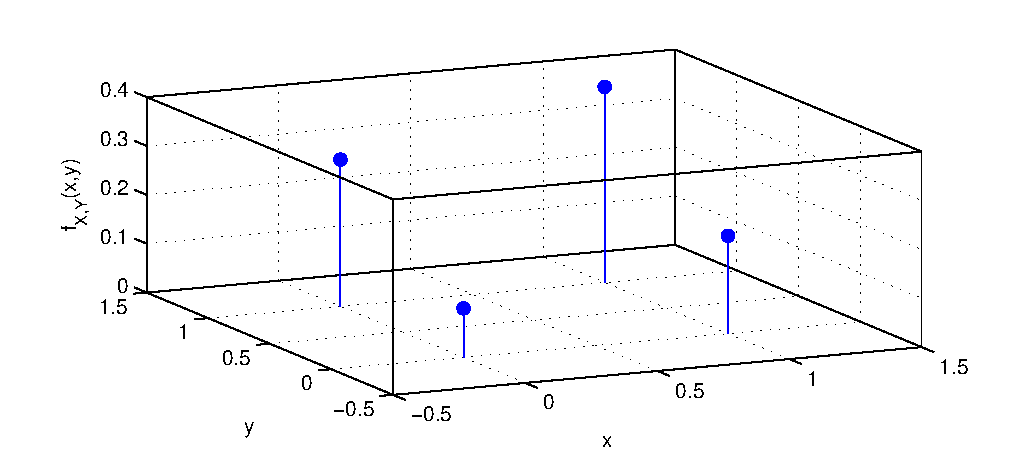
\includegraphics[width=5.0in]{figures/Discrete2DPMF}}
\end{center}
It is helpful to write down the JPMF $f_{X,Y}(x,y)$ in a tabular form:
\begin{center}
\begin{tabular}{|c|c c|}
\hline
& $Y=0$ & $Y=1$ \\ \hline
$X=0$& $0.1$ & $0.3$  \\
$X=1$& $0.2$ & $0.4$  \\ \hline
\end{tabular}
\end{center}
From the above Table we can read for instance that the joint probability $f_{X,Y}(0,0)=0.1$.

Find $\p(B)$ for the event $B=\{(0,0),(1,1)\}$, $F_{X,Y}(1/2,1/2)$, $F_{X,Y}(3/2,1/2)$, $F_{X,Y}(4,5)$ and $F_{X,Y}(-4,-1)$.

\begin{enumerate}
\item $\p(B) = \sum_{(x,y) \in \{(0,0),(1,1)\}}f_{X,Y}(x,y) = f_{X,Y}(0,0)+f_{X,Y}(1,1)=0.1+0.4$
\item $F_{X,Y}(1/2,1/2) = \sum_{\{(x,y): x\leq 1/2, y \leq 1/2\}} f_{X,Y}(x,y)=f_{X,Y}(0,0)=0.1$
\item $F_{X,Y}(3/2,1/2) = \sum_{\{(x,y): x\leq 3/2, y \leq 1/2\}} f_{X,Y}(x,y)=f_{X,Y}(0,0)+f_{X,Y}(1,0)=0.1+0.2=0.3$
\item $F_{X,Y}(4,5) = \sum_{\{(x,y): x\leq 4, y \leq 5\}} f_{X,Y}(x,y)=f_{X,Y}(0,0)+f_{X,Y}(0,1)+f_{X,Y}(1,0)+f_{X,Y}(1,1)=1$
\item $F_{X,Y}(-4,-1) = \sum_{\{(x,y): x\leq -4, y \leq -1\}} f_{X,Y}(x,y)=0$
\end{enumerate}
%\vspace{2cm}
\end{example}

\begin{definition}[JPDF] We say $(X,Y)$ is a {\bf continuous $\R^2$-valued random variable} if its JDF $F_{X,Y}(x,y)$ is differentiable and its {\bf joint probability density function (JPDF)} is given by:
\[
f_{X,Y}(x,y) = \frac{\partial^2}{\partial x \partial y} F_{X,Y}(x,y) \enspace .
\]
\end{definition}

For notational convenience, we sometimes suppress the subscripting when the random variables are clear from the context and write $f(x,y)$ and $F(x,y)$ instead of $f_{X,Y}(x,y)$ and $F_{X,Y}(x,y)$, respectively.

From JPDF $f_{X,Y}$ we can compute the JDF $F_{X,Y}$ at any point $(x,y) \in \Rz^2$ and more generally we can compute the probability of any event $B$, that can be cast as a region in $\Rz^2$, by simply taking two-dimensional integrals:
\begin{equation}\label{Eq:2ContjDFFromjPDF}
\boxed{F_{X,Y}(x,y) = \int_{-\infty}^{y} \int_{-\infty}^{x} f_{X,Y}(u,v) du dv}\enspace ,
\end{equation}
and
\begin{equation}\label{Eq:2ContProbEventFromjPDF}
\boxed{\p(B)\;=\; \int\int_{B} f_{X,Y}(x,y) dx dy}\enspace .
\end{equation}
In particular, if $\Bz_{\delta}(x,y)$ denotes a square of a small area $\delta>0$ that is centered at $(x,y)$, then the following approximate equality holds and improves as $\delta \to 0$:
\begin{equation}\label{Eq:2ContProbEventFromjPDFInSmallBall}
\p\left( (X,Y) \in \Bz_{\delta}(x,y) \right) \approxeq \delta f_{X,Y}(x,y) \enspace .
\end{equation}
The JPDF satisfies the following two properties:
\be
\item integrates to $1$, i.e., $\int_{-\infty}^{\infty} \int_{-\infty}^{\infty} f_{X,Y}(x,y) dx dy=1$
\item is a non-negative function, i.e., $f_{X,Y}(x,y) \geq 0$ for every $(x,y) \in \mathbb{R}^2$.
\ee

\begin{example}\label{Eg:Unif2DPDFandCDF}
Let $(X,Y)$ be a continuous \rv~that is uniformly distributed on the unit square $[0,1]^2 := [0,1] \times [0,1]$ with following JPDF:
\[
f(x,y) =  \BB{1}_{[0,1]^2}(x) 
\begin{cases}
1 & \text{ if } (x,y) \in [0,1]^2 \\
0 & \text{ otherwise}.
\end{cases}
\]
Find explicit expressions for the following: (1) DF $F(x,y)$ for any $(x,y) \in [0,1]^2$, (2) $\p(X \leq 1/3, Y \leq 1/2)$, (3) $P\left( (X,Y) \in [1/4,1/2]\times[1/3,2/3] \right)$.

\begin{center}
\makebox{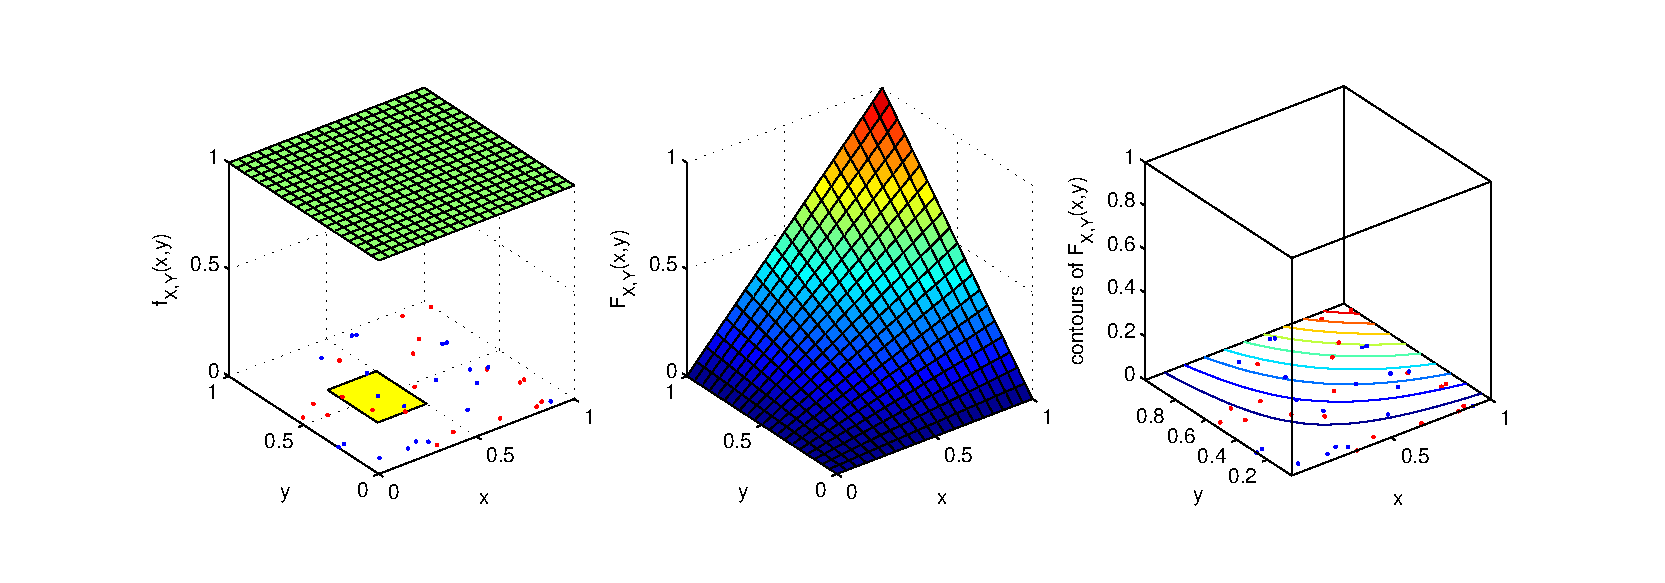
\includegraphics[width=6.5in]{figures/Unif2DPDFandCDF}}
\end{center}

Let us begin to find the needed expressions.
\be
\item
Let $(x,y) \in [0,1]^2$ then by Equation~\eqref{Eq:2ContjDFFromjPDF}:
{\small
\begin{align*}
F_{X,Y}(x,y) 
&= \int_{-\infty}^{y} \int_{-\infty}^{x} f_{X,Y}(u,v) dudv
= \int_{0}^{y} \int_{0}^{{x}} 1 dudv
= \int_{0}^{y} \left[ u \right]_{u=0}^{x}  dv
= \int_{0}^{y} x  dv
&= \left[ x v \right]_{v=0}^{y}
= {x}{y}
\end{align*}
}
\item We can obtain $\p(X \leq 1/3, Y \leq 1/2)$ by evaluating $F_{X,Y}$ at $(1/3,1/2)$:
{\small
\begin{align*}
\p(X \leq 1/3, Y \leq 1/2)
&= F_{X,Y}(1/3,1/2)
= \frac{1}{3}\frac{1}{2}
= \frac{1}{6}
\end{align*}
}
We can also find $\p(X \leq 1/3, Y \leq 1/2)$ by integrating the JPDF over the rectangular event $A=\{X < 1/3, Y < 1/2 \} \subset [0,1]^2$ according to Equation~\eqref{Eq:2ContProbEventFromjPDF}.  
This amounts here to finding the area of $A$, we compute $\p(A) = (1/3) (1/2) = 1/6$.  

\item We can find $P\left( (X,Y) \in [1/4,1/2]\times[1/3,2/3] \right)$ by integrating the JPDF over the rectangular event $B=[1/4,1/2]\times[1/3,2/3]$ according to Equation~\eqref{Eq:2ContProbEventFromjPDF}:
{\small
\begin{align*}
P\left( (X,Y) \in [1/4,1/2]\times[1/3,2/3] \right)
&=\int\int_B f_{X,Y}(x,y)dxdy
=\int_{1/3}^{2/3}\int_{1/4}^{1/2} 1 dx dy\\
&=\int_{1/3}^{2/3} \left[ x \right]_{1/4}^{1/2}  dy
=\int_{1/3}^{2/3} \left[ \frac{1}{2}-\frac{1}{4} \right]  dy
=\left(\frac{1}{2}-\frac{1}{4}\right)\left[ y \right]_{1/3}^{2/3}\\ 
&=\left(\frac{1}{2}-\frac{1}{4}\right)\left( \frac{2}{3}-\frac{1}{3} \right) 
=\frac{1}{4} \left( \frac{1}{3} \right) =\frac{1}{12}
\end{align*}
}
\ee

In general, for a bivariate uniform \rv~on the unit square the $\p([a,b]\times[c,d]) = (b-a)(d-c)$ for any event given by the rectangular region $[a,b]\times[c,d]$ inside the unit square $[0,1]\times[0,1]$.  
Thus any two events with the same rectangular area have the same probability (imagine sliding a small rectangle inside the unit square... no matter where you slide this rectangle to while remaining in the unit square, the probability of $\omega \mapsto (X(\omega),Y(\omega))=(x,y)$ falling inside this ``slidable'' rectangle is the same...).
\end{example}
 
\begin{example}\label{Eg:PlotPDF2ServerTimes}
Let the RV $X$ denote the time until a web server connects to your computer, and let the RV $Y$ denote the time until the server authorizes you as a valid user.  
Each of these RVs measures the waiting time from a common starting time (in milliseconds) and $X < Y$.  
From past response times of the web server we know that a good approximation for the JPDF of the \rv~$(X,Y)$ is
\[
f_{X,Y}(x,y) = 
\begin{cases}
\frac{6}{10^6} \exp \left( -\frac{1}{1000}x-\frac{2}{1000}y \right)
& \text{ if } x>0,y>0,x <y\\
0 & \text{ otherwise}.
\end{cases}
\]
Answer the following:
\be
\item identify the support of $(X,Y)$, i.e., the region in the plane where $f_{X,Y}$ takes positive values
\item check that $f_{X,Y}$ indeed integrates to $1$ as it should
\item Find $P(X \leq 400, Y \leq 800)$
\item It is known that humans prefer a response time of under $1/10$ seconds ($10^2$ milliseconds) from the web server before they get impatient.  What is $P(X+Y < 10^2)$? 
\ee
\begin{center}
\makebox{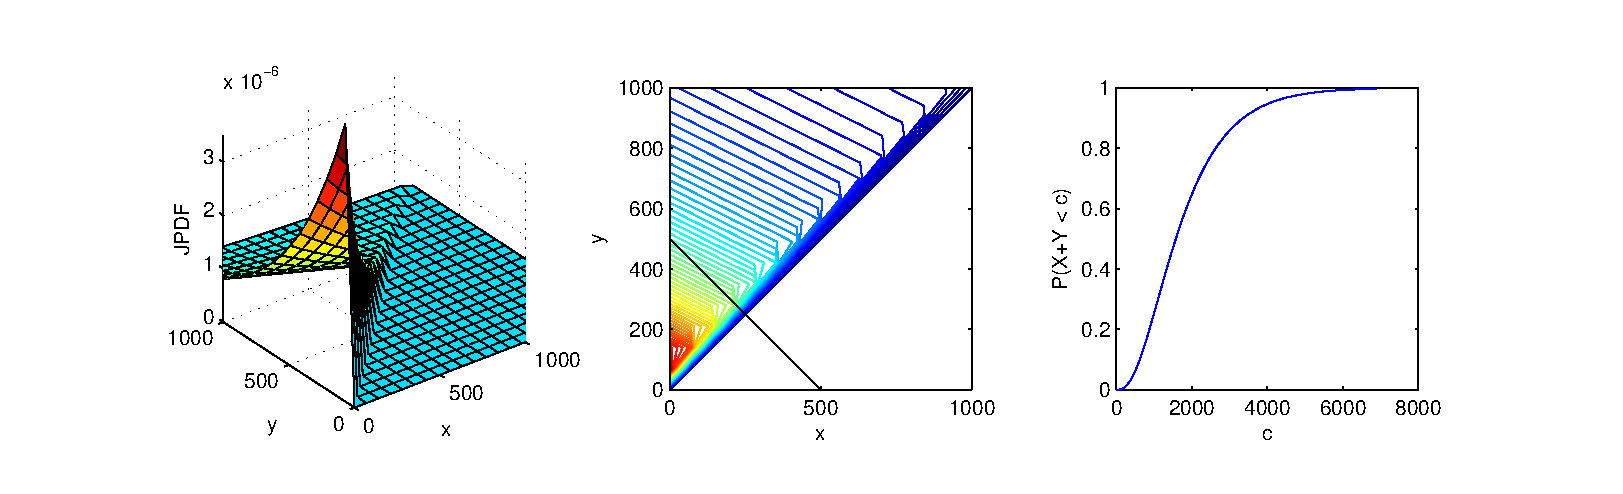
\includegraphics[width=6.0in]{figures/PlotPDF2ServerTimes}}
\end{center}
Let us answer the questions.
\be
\item
The support is the intersection of the positive quadrant with the $y>x$ half-plane.
\item
{\scriptsize
\begin{align*}
\int_{y=-\infty}^{\infty}\int_{x=-\infty}^{\infty} f_{X,Y}(x,y) dx dy 
&= \int_{x=0}^{\infty}\int_{y=x}^{\infty} f_{X,Y}(x,y) dy dx\\
&= \int_{x=0}^{\infty}\int_{y=x}^{\infty} \frac{6}{10^6} \exp \left( -\frac{1}{1000}x-\frac{2}{1000}y \right) dy dx\\
&= \frac{6}{10^6} \int_{x=0}^{\infty} \left(\int_{y=x}^{\infty} \exp \left( -\frac{2}{1000}y \right) dy \right) \exp \left(-\frac{1}{1000}x\right) dx\\
&= \frac{6}{10^6} \int_{x=0}^{\infty} \left[ -\frac{1000}{2} \exp \left( -\frac{2}{1000}y \right) \right]_{y=x}^{\infty}  \exp \left(-\frac{1}{1000}x\right) dx\\
&= \frac{6}{10^6} \int_{x=0}^{\infty} \left[0 +\frac{1000}{2}\exp \left( -\frac{2}{1000}x \right) \right]  \exp \left(-\frac{1}{1000}x\right) dx\\
&= \frac{6}{10^6} \int_{x=0}^{\infty} \frac{1000}{2}\exp \left( -\frac{2}{1000}x -\frac{1}{1000}x\right) dx\\
&= \frac{6}{10^6} \frac{1000}{2} \left[ -\frac{1000}{3} \exp \left(-\frac{3}{1000}x\right)\right]_{x=0}^{\infty} \\
&= \frac{6}{10^6} \frac{1000}{2} \left[0 +\frac{1000}{3} \right] \\
&=1
\end{align*}
}
\item
First, identify the region with positive JPDF for the event $(X \leq 400, Y \leq 800)$
{\scriptsize
\begin{align*}
&P(X \leq 400, Y \leq 800)\\
&= \int_{x=0}^{400} \int_{y=x}^{800} f_{X,Y}(x,y) dy dx \\
&= \int_{x=0}^{400} \int_{y=x}^{800} \frac{6}{10^6} \exp \left( -\frac{1}{1000}x-\frac{2}{1000}y \right) dy dx \\
&= \frac{6}{10^6}  \int_{x=0}^{400} \left[ -\frac{1000}{2} \exp \left( -\frac{2}{1000}y \right) \right]_{y=x}^{800}  \exp \left(-\frac{1}{1000}x\right) dx\\
&= \frac{6}{10^6} \frac{1000}{2} \int_{x=0}^{400} \left( - \exp \left( -\frac{1600}{1000} \right) + \exp \left( -\frac{2}{1000}x \right) \right)  \exp \left(-\frac{1}{1000}x\right) dx\\
&= \frac{6}{10^6} \frac{1000}{2} \int_{x=0}^{400} \left( \exp \left( -\frac{3}{1000}x \right) - e^{-8/5} \exp \left(-\frac{1}{1000}x\right)\right) dx\\
&= \frac{6}{10^6} \frac{1000}{2} \left( \left( -\frac{1000}{3} \exp \left( -\frac{3}{1000}x \right) \right)_{x=0}^{400} - e^{-8/5} \left(-1000 \exp \left(-\frac{1}{1000}x\right)\right)_{x=0}^{400} \right) \\
&= \frac{6}{10^6} \frac{1000}{2} 1000 \left( \frac{1}{3}\left(1- e^{-6/5} \right) - e^{-8/5} \left( 1-e^{-2/5}\right) \right) \\
&= 3 \left( \frac{1}{3}\left(1- e^{-6/5} \right) - e^{-8/5} \left( 1-e^{-2/5}\right) \right) \\
&\approxeq 0.499 \enspace .
\end{align*}
}
\item
First, identify the region with positive JPDF for the event $(X+Y \leq c)$, say $c=500$ (but generally $c$ can be any positive number).
This is the triangular region at the intersection of the four half-planes: $x>0$, $x < c$, $y>x$ and $y<c-x$. ({\em Draw picture here})
%\vspace{2cm}\\
Let's integrate the JPDF over our triangular event as follows:
{\scriptsize
\begin{align*}
P(X+Y \leq c) 
&= \int_{x=0}^{c/2}\int_{y=x}^{c-x} f_{X,Y}(x,y) dy dx \\
&= \int_{x=0}^{c/2}\int_{y=x}^{c-x} \frac{6}{10^6} \exp \left( -\frac{1}{1000}x-\frac{2}{1000}y \right) dy dx \\
&= \frac{6}{10^6} \int_{x=0}^{c/2}\int_{y=x}^{c-x}  \exp \left( -\frac{1}{1000}x-\frac{2}{1000}y \right) dy dx \\
&= \frac{6}{10^6} \frac{1000}{2} \int_{x=0}^{c/2} \left[ - \exp \left( -\frac{2}{1000}y \right) \right]_{y=x}^{c-x}  \exp \left(-\frac{1}{1000}x\right) dx\\
&= \frac{3}{10^3} \int_{x=0}^{c/2} \left[ - \exp \left( -\frac{2c-2x}{1000} \right) + \exp \left( -\frac{2x}{1000} \right) \right]  \exp \left(-\frac{x}{1000}\right) dx\\
&= \frac{3}{10^3} \int_{x=0}^{c/2} \left(  \exp \left( -\frac{3x}{1000} \right) - \exp \left( \frac{x-2c}{1000} \right) \right)  dx\\
&= 3 \left( \left[-\frac{1}{3} \exp \left( -\frac{3x}{1000} \right) \right]_{x=0}^{c/2} - \left[ e^{-2c/1000} \exp \left( \frac{x}{1000} \right)\right]_{x=0}^{c/2} \right)  \\
&= 3  \left(\frac{1}{3} (1-e^{-3c/2000}) - e^{-2c/1000} (e^{c/2000}-1) \right)\\
&= 1 - e^{-3c/2000} + 3 e^{-2c/1000} - 3 e^{-3c/2000}\\
&= 1 - 4 e^{-3c/2000} + 3 e^{-c/500}
\end{align*}
}
%\vspace{1cm}\\
\item $P(X+Y<100) = 1 - 4 e^{-300/2000} + 3 e^{-100/500} \approxeq 0.134$.  This means only about one in one hundred requests to this server will be processed within 100 milliseconds.
\ee
We can obtain $P(X+Y<c)$ for several values of $c$ using \Matlab and note that about 96\% of requests are processed in less than 3000 milliseconds or 3 seconds.
\begin{VrbM}
>> c = [100 1000 2000 3000 4000]
c =  100        1000        2000        3000        4000

>> p = 1 - 4 * exp(-3*c/2000) + 3 * exp(-c/500)

p =  0.0134     0.5135      0.8558      0.9630      0.9911
\end{VrbM}
\end{example}

\begin{definition}[Marginal PDF or PMF]
If the \rv~$(X,Y)$ has $f_{X,Y}(x,y)$ as its joint PDF or joint PMF, then the 
{\bf marginal PDF or PMF} of a random vector $(X,Y)$ is defined by :
\[
f_{X}(x) =
\begin{cases}
\int_{-\infty}^{\infty} f_{X,Y}(x,y) dy & \text{if $(X,Y)$ is a continuous \rv}  \\
\sum_{y} f_{X,Y}(x,y) & \text{if $(X,Y)$ is a discrete \rv} \\
\end{cases}
\]
and the  {\bf marginal PDF or PMF} of $Y$ is defined by:
\[
f_{Y}(y) = 
\begin{cases}
\int_{-\infty}^{\infty} f_{X,Y}(x,y) dx & \text{if $(X,Y)$ is a continuous \rv}  \\
\sum_{x} f_{X,Y}(x,y) & \text{if $(X,Y)$ is a discrete \rv} \\
\end{cases}
\]
\end{definition}

\begin{example}
Obtain the marginal PMFs $f_Y(y)$ and $f_X(x)$ from the joint PMF $f_{X,Y}(x,y)$ of the discrete \rv~in \hyperref[Eg:Discrete2DPMF]{Example~\ref*{Eg:Discrete2DPMF}}.
Just sum $f_{X,Y}(x,y)$ over $x$'s and $y$'s (reported in a tabular form):
\begin{center}
\begin{tabular}{|c|c c|}
\hline
& $Y=0$ & $Y=1$ \\ \hline
$X=0$& $0.1$ & $0.3$  \\
$X=1$& $0.2$ & $0.4$  \\ \hline
\end{tabular}
\end{center}
From the above Table we can find:
\begin{align*}
f_X(x) = P(X=x) 
&= \sum_{y} f_{X,Y}(x,y) \\
&= 
f_{X,Y}(x,0) + f_{X,Y}(x,1) = 
\begin{cases}
f_{X,Y}(0,0) + f_{X,Y}(0,1) = 0.1+0.3=0.4 & \text{ if } x=0\\
f_{X,Y}(1,0) + f_{X,Y}(1,1) = 0.2+0.4=0.6 & \text{ if } x=1\\
\end{cases}
\end{align*}
Similarly,
\begin{align*}
f_Y(y) = P(Y=y) 
&= \sum_{x} f_{X,Y}(x,y) \\
&= 
f_{X,Y}(0,y) + f_{X,Y}(1,y) 
= 
\begin{cases}
f_{X,Y}(0,0) + f_{X,Y}(1,0) = 0.1+0.2=0.3 & \text{ if } y=0\\
f_{X,Y}(0,1) + f_{X,Y}(1,1) = 0.3+0.4=0.7 & \text{ if } y=1\\
\end{cases}
\end{align*}
Just report the marginal probabilities as row and column sums of the JPDF table.

Thus marginal PMF gives us the probability of a specific RV, within a \rv, taking a value irrespective of the value taken by the other RV in this \rv. 
\end{example}

\begin{example}
Obtain the marginal PDFs $f_Y(y)$ and $f_X(x)$ from the joint PDF $f_{X,Y}(x,y)$ of the continuous \rv~in \hyperref[Eg:Unif2DPDFandCDF]{Example~\ref*{Eg:Unif2DPDFandCDF}} (the bivariate uniform \rv~on $[0,1]^2$).

\begin{center}
\makebox{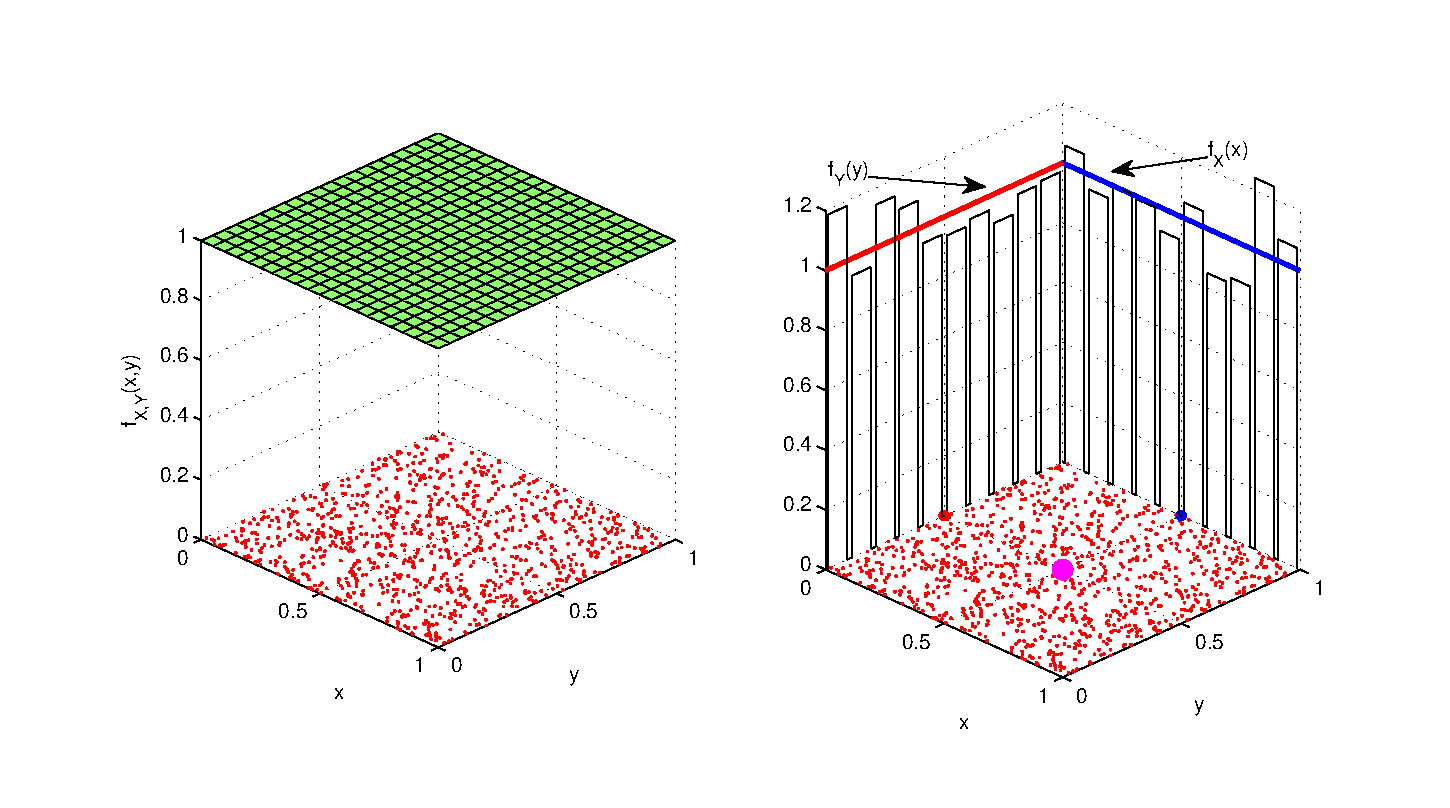
\includegraphics[width=6.0in]{figures/PlotPDFSamplesMarginalsUnif2D}}
\end{center}

Let us suppose $(x,y) \in [0,1]^2$ and note that $f_{X,Y}=0$ if $(x,y) \notin [0,1]^2$.  
We can obtain marginal PMFs $f_X(x)$ and $f_Y(y)$ by integrating the JPDF $f_{X,Y}=1$ along $y$ and $x$, respectively.
\[
f_X(x) = \int_{-\infty}^{\infty} f_{X,Y}(x,y) dy = \int_{0}^{1} f_{X,Y}(x,y) dy 
= \int_{0}^{1} 1 dy = \left[ y \right]_0^1 = 1-0 = 1
\]
Similarly,
\[
f_Y(y) = \int_{-\infty}^{\infty} f_{X,Y}(x,y) dx = \int_{0}^{1} f_{X,Y}(x,y) dx 
= \int_{0}^{1} 1 dx = \left[ x \right]_0^1 = 1-0 = 1
\]
We are seeing a histogram of the {\bf marginal samples} and their marginal PDFs in the Figure.
\end{example}

Thus marginal PDF gives us the probability density of a specific RV in a \rv, irrespective of the value taken by the other RV in this \rv. 

\begin{example}
Obtain the marginal PDF $f_Y(y)$ from the joint PDF $f_{X,Y}(x,y)$ of the continuous \rv~in \hyperref[Eg:PlotPDF2ServerTimes]{Example~\ref*{Eg:PlotPDF2ServerTimes}} that gave the response times of a web server.
\[
f_{X,Y}(x,y) = 
\begin{cases}
\frac{6}{10^6} \exp \left( -\frac{1}{1000}x-\frac{2}{1000}y \right)
& \text{ if } x>0,y>0,x <y\\
0 & \text{ otherwise}.
\end{cases}
\]
Use $f_Y(y)$ to compute the probability that $Y$ exceeds 2000 milliseconds.

%\vspace{5in}
First we need to obtain an expression for $f_Y(y)$. For $y > 0$,
{\scriptsize
\begin{align*}
f_Y(y) 
&= \int_{x=-\infty}^{\infty} f_{X,Y}(x,y) dx\\
&= \int_{x=-\infty}^{\infty} 6 \times 10^{-6} e^{-0.001 x - 0.002y} dx\\
&= 6 \times 10^{-6} \int_{x=0}^{y} e^{-0.001 x - 0.002y} dx\\ 
&= 6 \times 10^{-6} e^{-0.002y} \int_{x=0}^{y}  e^{-0.001 x} dx\\ 
&= 6 \times 10^{-6} e^{-0.002y} \left[ \frac{e^{-0.001 x}}{-0.001}\right]_{x=0}^{x=y}\\ 
&= 6 \times 10^{-6} e^{-0.002y} \left( \frac{e^{-0.001 y}}{-0.001} - \frac{e^{-0.001 \times 0}}{-0.001} \right)\\ 
&= 6 \times 10^{-6} e^{-0.002y} \left( \frac{1- e^{-0.001 y}}{0.001} \right)\\ 
&= 6 \times 10^{-3} e^{-0.002y} \left({1- e^{-0.001 y}} \right)\\ 
\end{align*}
}
We have the marginal PDF of $Y$ and from this we can obtain 
{\scriptsize
\begin{align*}
P(Y>2000)
&= \int_{2000}^{\infty} f_Y(y) dy \\
&= \int_{2000}^{\infty} 6 \times 10^{-3} e^{-0.002y} \left({1- e^{-0.001 y}} \right) dy\\
&= 6 \times 10^{-3} \int_{2000}^{\infty}  e^{-0.002y} dy - \int_{2000}^{\infty} e^{-0.003 y} dy\\
&= 6 \times 10^{-3} \left( \left[ \frac{e^{-0.002y}}{-0.002} \right]_{2000}^{\infty} 
- \left( \left[ \frac{e^{-0.003y}}{-0.003} \right]_{2000}^{\infty} \right) \right)\\
&= 6 \times 10^{-3} \left( \frac{e^{-4}}{0.002} - \frac{e^{-6}}{0.003} \right)\\
&= 0.05
\end{align*}
}

{\scriptsize
Alternatively, you can obtain $P(Y>2000)$ by directly integrating the joint PDF $f_{X,Y}(x,y)$ over the appropriate region (but you may now have to integrate two pieces: rectangular infinite strip ${(x,y): 0<x<2000, y>2000}$ and a triangular infinite piece $\{(x,y): y>x, y>2000, x> 2000\}$)... more involved but we get the same answer.
\begin{multline*}
P(Y>2000) = \int_{x=0}^{2000} \left( \int_{y=2000}^{\infty} 6 \times 10^{-6} e^{-0.001 x - 0.002y} dy \right) dx + \\
\int_{x=2000}^{\infty} \left( \int_{y=x}^{\infty} 6 \times 10^{-6} e^{-0.001 x - 0.002y} dy \right) dx 
\\
\vdots \text{(try as a tutorial problem)} \\
P(Y>2000) = 0.0475 + 0.0025 = 0.05
\end{multline*}
}
\end{example}

We have seen the notion of independnece of two events in \hyperref[D:IndOf2Events]{Definition~\ref*{D:IndOf2Events}} or of a sequence of events in \hyperref[D:IndOfSeqOfEvents]{Definition~\ref*{D:IndOfSeqOfEvents}}. 
Recall that independence amounts to having the probability of the joint occurrence of the events to be given by the product of the probabilities of each of the events.

We can use the definition of independence of two events to define the independence of two random variables using their distribution functions.

\begin{definition}[Independence of Two RVs]\label{D:Ind2RVs}
Consider an $\Rz^2$-valued RV $X:=(X_1,X_2)$. Then the $\Rz$-valued RVs $X_1$ and $X_2$ are said to be independent or independently distributed if and only if
\[
\p(X_{1} \leq x_{1}, X_{2} \leq x_{2} ) = \p(X_{1} \leq x_{1}) \p(X_{2} \leq x_{2})
\]
or equivalently,
\[
F_{X_{1},X_{2}}(x_{1},x_{2}) = F_{X_{1}}(x_{1}) F_{X_{2}}(x_{2}) \enspace ,
\]
for any pair of real numbers $(x_{1},x_{2}) \in \Rz^2$.

By the above definition, for {\bf discrete} RVs $X_1,X_2$ that are independent, the following equality is satisfied between the joint and marginal PMFs:
\[
f_{X_1,X_2}(x_1,x_2) = \p(X_{1}= x_{1}, X_{2} = x_{2}) = \p(X_{1} = x_{1}) \p(X_{2} = x_{2}) = f_{X_1}(x_1) f_{X_2}(x_2) \text{ for any} (x_{1},x_{2}) \in \Rz^2 \enspace ,
\]
and for {\bf continuous} RVs $X_1,X_2$ that are independent, the following equality is satisfied between the joint and marginal PDFs:
\[
f_{X_1,X_2}(x_1,x_2) = f_{X_1}(x_1) f_{X_2}(x_2)  \text{ for any} (x_{1},x_{2}) \in \Rz^2 \enspace .
\] 
\end{definition}

In summary, two RVs $X$ and $Y$ are said to be {\bf independent} if and only if for every $(x,y)$
\[
\boxed{
F_{X,Y}(x,y) = F_X(x) \times F_Y(y) \qquad \text{ or } f_{X,Y}(x,y) = f_X(x) \times f_Y(y)
}
\]

Let us confirm that our familiar experiment of tossing a fair coin twice independently when encoded by a pair of independent $\bernoulli(1/2)$ RVs satisfies the above definition.
\begin{example}[Pair of independent $\bernoulli(1/2)$ RVs]
Let $X_1$ and $X_2$ be a pair of independent $\bernoulli(1/2)$ RVs each taking values in the set $\{0,1\}$ with the following tabulated probabilities. Verify that the JPMF $f_{X_1,X_2}(x_1,x_2)=1/4$ for each $(x_1,x_2) \in \{0,1\}^2$ is indeed given by the marginal PMF $f_{X_i}(x_i)=1/2$ for each $i \in \{1,2\}$ and each $x_i \in \{0,1\}$.

\begin{center}
\begin{tabular}{|c|c c|c|}
\hline
& $X_2=0$ & $X_2=1$ & \\ \hline
$X_1=0$& $1/4$ & $1/4$ & $1/2$ \\
$X_1=1$& $1/4$ & $1/4$ & $1/2$ \\ \hline
& $1/2$ & $1/2$ & $1$\\ \hline
\end{tabular}
\end{center}
From the above Table we can read for instance that the {\em joint probability} that $\Rz^2$-valued RV $(X_1,X_2)$ takes the value or realization $(0,0)$ is $1/4$ from the first entry of the inner-most tabulated rectangle, 
i.e., $\p((X_1,X_2)=(0,0))=1/4$, 
and that the {\em marginal probability} that the RV $X_1$ takes the value or relaization $0$ is $1/2$, 
i.e., $\p(X_1=0)=1/2$. 
Clearly, $1/4=1/2 \times 1/2$, and so our familiar experiment when seen as an $\Rz^2$-valued RV is indeed composed of two independent$\Rz$-valued $\bernoulli(1/2)$ RVs. 
\end{example}

\begin{example}
Recall the $\Rz^2$-valued continuous RV $(X,Y)$ of \hyperref[Eg:Unif2DPDFandCDF]{Example~\ref*{Eg:Unif2DPDFandCDF}} 
that is uniformly distributed on the unit square $[0,1]^2$. 
First show that $X$ and $Y$ independent. 
Then show that both $X$ and $Y$ are identically distributed according to the $\uniform(0,1)$ RV. 

This can be shown by checking that the joint PDF is indeed equal to the product of the marginal PDFs of $\uniform(0,1)$ RVs as follows:
\[
\begin{cases}
1= f_{X,Y}(x,y) =  f_X(x) \times f_Y(y) = 1 \times 1 = 1 & \text{ if } (x,y) \in [0,1]^2\\
0= f_{X,Y}(x,y) =  f_X(x) \times f_Y(y) = 0 \times 0 = 0 & \text{ if } (x,y) \notin [0,1]^2
\end{cases}
\]
\end{example}

Are $X$ and $Y$ independent in the server times \rv~from \hyperref[Eg:PlotPDF2ServerTimes]{Example~\ref*{Eg:PlotPDF2ServerTimes}}?

We can compute $f_X(x)$ and use the already computed $f_Y(y)$ to mechanically check if the JPDF is the product of the marginal PDFs.  But intuitively, we know that these RVs (connection time and authentication time) are dependent -- one is strictly greater than the other.  
Also the JPDF has zero density when $x>y$, but the product of the marginal densities won't.

Now, let us take advantage of independent random variables and solve some problems.

\begin{example}[distance between random faults in a manufactured line]
Suppose two points are tossed independently and uniformly at random onto a line segment of unit length.  
What is the probability that the distance between the two points does not exceed a given length $l$? 

\vspace{5cm}
done in lectures...

\end{example}

Let us introduce parameters for the lower and upper bounds of the interval upon which a continuous RV is uniformly distributed using the following probability model.
 
\begin{model}[$\uniform(\theta_1,\theta_2)$]\label{M:Uniformab}
Given two real parameters $\theta_1,\theta_2 \in \Rz$, such that $\theta_1 < \theta_2$, the PDF of the $Uniform(\theta_1,\theta_2)$ RV $X$ is:
\begin{equation}\label{E:Uniformabpdf}
f(x;\theta_1,\theta_2) =
\begin{cases}
\frac{1}{\theta_2 - \theta_1} & \text{if $\theta_1 \leq x \leq \theta_2$,}\\
0 & \text{otherwise}
\end{cases}
\end{equation}
and its DF given by $F(x;\theta_1,\theta_2) = \int_{- \infty}^x f(y; \theta_1,\theta_2) \, dy$ is:
\begin{equation}\label{E:Uniformabcdf}
F(x; \theta_1,\theta_2) =
\begin{cases}
0 & \text{if $x < \theta_1$} \\
\frac{x-\theta_1}{\theta_2-\theta_1} & if~\theta_1 \leq x \leq \theta_2,\\
1 & \text{if $x > \theta_2$}
\end{cases}
\end{equation}
Recall that we emphasise the dependence of the probabilities on the two parameters $\theta_1$ and $\theta_2$ by specifying them following the semicolon in the argument for $f$ and $F$.
\end{model}
\begin{figure}[htpb]
\caption{A plot of the PDF, DF or CDF and inverse DF of the $\uniform(-1,1)$ RV $X$.\label{F:unifpm1}}
\centering   \makebox{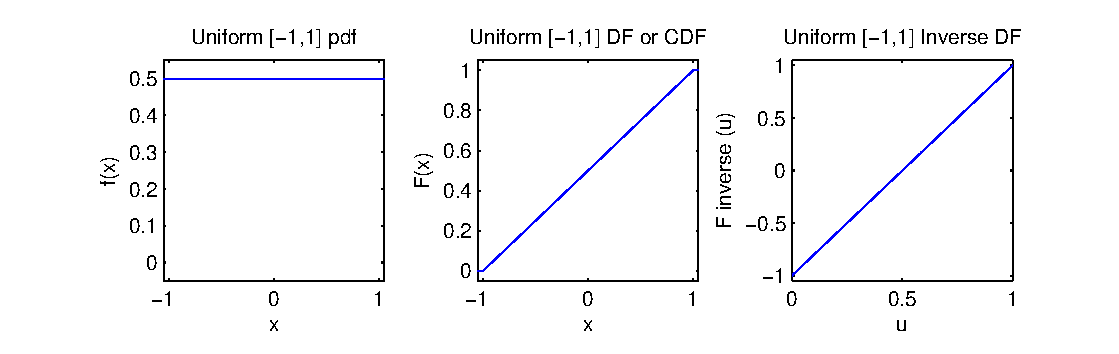
\includegraphics[width=6.5in]{figures/Unifpm1pdfcdf}}
\end{figure}
\begin{example}[Buffon's Needle Experiment to Physically Estimate $\pi$]
~

done in lectures...
\vspace{5cm}

\end{example}

\subsection{Conditional Random Variables}

Often we will have a condition where one of the two random variables that make up a random vector $(X_1,X_2)$ already occurs and takes a value. 
And we might want to compute the probability of the occurrence of the other random variable given this conditional information.
For this all we need to do is extend the idea of conditional probabiliies to $\Rz^2$-valued random variables as defined below.

\begin{definition}[Conditional PDF or PMF]
Let $(X_1,X_2)$ be a discrete bivariate \rv.  The conditional PMF of $X_1|X_2=x_2$, where $f_{X_2}(x_2) := \p(X_2=x_2) > 0$ is:
\[
f_{X_1|X_2}(x_1 | x_2) := \p(X_1=x_1 | X_2=x_2) = \frac{\p(X_1=x_1,X_2=x_2)}{\p(X_2=x_2)} = \frac{f_{X_1,X_2}(x_1,x_2)}{f_{X_2}(x_2)} \ .
\]
Similarly, if $f_{X_1}(x_1) := \p(X_1=x_1) >0$, then the conditional PMF of $X_2|X_1=x_1$ is:
\[
f_{X_2|X_1}(x_2|x_1) := \p(X_2=x_2 | X_1=x_1) = \frac{\p(X_1=x_1,X_2=x_2)}{\p(X_1=x_1)} = \frac{f_{X_1,X_2}(x_1,x_2)}{f_{X_1}(x_1)} \ .
\]
If $(X_1,X_2)$ are continuous RVs such that the marginal PDF $f_{X_2}(x_2)>0$, then the conditional PDF of $X_1|X_2=x_2$ is:
\[
f_{X_1|X_2}(x_1|x_2) = \frac{f_{X_1,X_2}(x_1,x_2)}{f_{X_2}(x_2)}, \qquad \p(X_1 \in A| X_2=x_2) = \int_A f_{X_1|X_2}(x_1|x_2) dx_1 \ .
\]
Similarly, if $f_{X_1}(x_1)>0$, then the conditional PDF of $X_2|X_1=x_1$ is:
\[
f_{X_2|X_1}(x_2|x_1) = \frac{f_{X_1,X_2}(x_1,x_2)}{f_{X_1}(x_1)}, \qquad \p(X_2 \in A| X_1=x_1) = \int_A f_{X_2|X_1}(x_2|x_1) dx_2 \ .
\]
\end{definition}

Let us consider a few discrete RVs for the simple coin tossing experiment $\E{E}_{\theta}^{3}$ that build on the $\bernoulli(\theta)$ RV $X_i$ for the $i$-th toss in an {\bf independent and identically distibuted (IID.)} manner.
\begin{table}[htpb]
\caption{The $8$ $\omega$'s in the sample space $\Omega$ of the experiment $\E{E}_{\theta}^{3}$ are given in the first row above.  The RV $Y$ is the number of `Heads' in the $3$ tosses and the RV $Z$ is the number of `Tails' in the $3$ tosses.  Finally, the RVs $Y'$ and $Z'$ are the indicator functions of the event that `all three tosses were Heads' and the event that `all three tosses were Tails', respectively.\label{T:T3XRVs}}
 \begin{tabular}{r c c c c c c c c l}
 \hline
$\omega$:    & {\tt HHH} & {\tt HHT} & {\tt HTH} & {\tt HTT} & {\tt THH} & {\tt THT} & {\tt TTH} & {\tt TTT} & RV Definitions / Model \\ \hline
 \\
$\p(\omega)$: & $\frac{1}{8}$ & $\frac{1}{8}$ & $\frac{1}{8}$ & $\frac{1}{8}$ &  $\frac{1}{8}$ & $\frac{1}{8}$ & $\frac{1}{8}$ & $\frac{1}{8}$  & $X_i \overset{\IID}{\sim} \bernoulli(\frac{1}{2})$ \\
 \\
$Y(\omega)$: & 3         & 2         & 2         & 1         & 2         & 1         & 1         & 0        & $Y := X_1+X_2+X_3$ \\
 \\
$Z(\omega)$: & 0         & 1         & 1         & 2         & 1         & 2         & 2         & 3        & $Z := (1-X_1)+(1-X_2)+(1-X_3)$ \\
 \\
$Y'(\omega)$: & 1         & 0         & 0         & 0         & 0         & 0         & 0         & 0       & $Y' :=  X_1 X_2 X_3$ \\
\\
$Z'(\omega)$: & 0         & 0         & 0         & 0         & 0         & 0         & 0         & 1       & $Y' :=  (1-X_1)(1-X_2)(1-X_3)$ \\ \hline
 \end{tabular}
 \end{table}
 \begin{classwork}[Two random variables of `toss a coin thrice' experiment]
Describe the probability of the RV $Y$ and $Y'$ of \hyperref[T:T3XRVs]{Table \ref*{T:T3XRVs}} in terms of its PMF.  Repeat the process for the RV $Z$ in your spare time.
 \begin{eqnarray}
 \p(Y=y) =%:= \p(\{\omega: Y(\omega)=y\}) = 
 \begin{cases}
 \qquad & \qquad \notag \\
 \qquad & \qquad \notag \\
 \qquad & \qquad \notag \\
 \qquad & \qquad \notag
 \end{cases} 
 & \qquad \qquad \qquad \qquad \qquad
\p(Y'=y') =%:= \p(\{\omega: Y'(\omega)=y'\}) = 
 \begin{cases}
 \qquad & \qquad \notag \\
 \qquad & \qquad \notag 
 \end{cases}
 \end{eqnarray}
 \end{classwork}
 
 \begin{classwork}[The number of `Heads' given there is at least one `Tails']
 Consider the following two questions.
 \begin{enumerate}
\item What is conditional probability $\p(Y|Y'=0)$ ?
%{\color{Gray}{
 \[
 \begin{array}{c c c c}
 \hline \\
 \p(Y=y | Y'=0) & =\frac{\p(Y=y,Y'=0)}{\p(Y'=0)} & =\frac{\p(\{\omega: Y(\omega)=y \  \cap \ Y'(\omega)=0\})}{\p(\{\omega: Y'(\omega)=0\})} & = ? \\ \hline \\
 \\
 \p(Y=0 | Y'=0) & \frac{\p(Y=0,Y'=0)}{\p(Y'=0)} & \frac{\frac{1}{8}}{\frac{1}{8}+\frac{1}{8}+\frac{1}{8}+\frac{1}{8}+\frac{1}{8}+\frac{1}{8}+\frac{1}{8}} & \frac{1}{7} \\
\\
\p(Y=1 | Y'=0) & \frac{\p(Y=1,Y'=0)}{\p(Y'=0)} & \frac{\frac{1}{8}+\frac{1}{8}+\frac{1}{8}}{\frac{1}{8}+\frac{1}{8}+\frac{1}{8}+\frac{1}{8}+\frac{1}{8}+\frac{1}{8}+\frac{1}{8}} & \frac{3}{7} \\
\\
\p(Y=2 | Y'=0) & \frac{\p(Y=2,Y'=0)}{\p(Y'=0)} & \frac{\frac{1}{8}+\frac{1}{8}+\frac{1}{8}}{\frac{1}{8}+\frac{1}{8}+\frac{1}{8}+\frac{1}{8}+\frac{1}{8}+\frac{1}{8}+\frac{1}{8}} & \frac{3}{7} \\
\\
\p(Y=3 | Y'=0) & \frac{\p(Y=3,Y'=0)}{\p(Y'=0)} & \frac{\p(\emptyset)}{\frac{1}{8}+\frac{1}{8}+\frac{1}{8}+\frac{1}{8}+\frac{1}{8}+\frac{1}{8}+\frac{1}{8}} & 0 \\
\\ \hline
\p(Y \in \{0,1,2,3\} | Y'=0) & \frac{\sum_{y=0}^3{\p(Y=y,Y'=0)}}{\p(Y'=0)} & \frac {\frac{1}{8}+\frac{1}{8}+\frac{1}{8}+\frac{1}{8}+\frac{1}{8}+\frac{1}{8}+\frac{1}{8}}{\frac{1}{8}+\frac{1}{8}+\frac{1}{8}+\frac{1}{8}+\frac{1}{8}+\frac{1}{8}+\frac{1}{8}} & 1 \\ \hline
 \end{array}
 \]
% }}
\item What is $\p(Y|Y'=1)$ ?
%{\color{Gray}{
 \[
\p(Y=y | Y'=1) = 
\begin{cases}
1 & \text{if $y=3$} \\
0 & \text{otherwise}
 \end{cases}
 \]
 %}}
 \end{enumerate}
 \end{classwork}

\subsection{$\Rz^m$-valued Random Variables}

%Extension to multivariate random vectors that are made of more than two RVs is straightforward.  
Consider the \rv~ $X$ whose components are the RVs $X_1,X_2,\ldots,X_m$, i.e., $X := (X_1,X_2,\ldots,X_m)$, where $m \geq 2$.  
A particular realization of this RV is a point $(x_1,x_2,\ldots,x_m)$ in $\Rz^m$.  
Now, let us extend the notions of JCDF, JPMF and JPDF to $\Rz^m$.  

\begin{definition}[multivariate JDF]\label{Df:JmDF}
The {\bf joint distribution function (JDF)} or {\bf joint cumulative distribution function (JCDF)}, $F_{X_1,X_2,\ldots,X_m}(x_1,x_2,\ldots,x_m):\mathbb{R}^m\to [0,1]$, of the multivariate random vector $(X_1,X_2,\ldots,X_m)$ is
\begin{eqnarray}\label{E:jmDF}
F_{X_1,X_2,\ldots,X_m}(x_1,x_2,\ldots,x_m)\; 
&=& P(X\leq x_1 \cap X_2 \leq x_2 \cap \cdots \cap X_m \leq x_m)\notag\\ 
&=& P(X_1\leq x_1 , X_2 \leq x_2, \ldots, X_m \leq x_m)\\
&=& P\left( \{ \omega: X_1(\omega) \leq x_1, X_2(\omega) \leq x_2, \ldots, X_m(\omega) \leq x_m \} \right), \notag
\end{eqnarray}
for any $(x_1,x_2,\ldots,x_m) \in \mathbb{R}^m$, 
where the right-hand side represents the probability that the random vector $(X_1,X_2,\ldots,X_m)$ takes on a value in 
$\{(x'_1,x'_2,\ldots,x'_m): x'_1 \leq x_1, x'_2 \leq x_2, \ldots, x'_m \leq x_m\}$, the set of points in $\Rz^m$ that are less than the point $(x_1,x_2,\ldots,x_m)$ in each coordinate $1,2,\ldots,m$.
\end{definition}

The JDF $F_{X_1,X_2,\ldots,X_m}(x_1,x_2,\ldots,x_m):\Rz^m\to\Rz$ satisfies the following conditions to remain a probability: 
\begin{enumerate}
\item $0 \leq F_{X_1,X_2,\ldots,X_m}(x_1,x_2,\ldots,x_m) \leq 1$
\item $F_{X_1,X_2,\ldots,X_m}(x_1,x_2,\ldots,x_m)$ is an increasing function of $x_1$, $x_2$, $\ldots$ and $x_m$
\item $F_{X_1,X_2,\ldots,X_m}(x_1,x_2,\ldots,x_m) \to 1$ as $x_1\to \infty$, $x_2\to \infty$, $\ldots$ and $x_m\to \infty$
\item $F_{X_1,X_2,\ldots,X_m}(x_1,x_2,\ldots,x_m) \to 0$ as $x_1\to -\infty$, $x_2\to -\infty$, $\ldots$ and $x_m\to -\infty$
\end{enumerate}

\begin{definition}[Multivariate JPMF]
If $(X_1,X_2,\ldots,X_m)$ is a {\bf discrete random vector} that takes values in a discrete support set $\mathcal{S}_{X_1,X_2,\ldots,X_m}$, then its \textbf{joint probability mass function} (or JPMF) is:
\begin{equation}\label{Eq:jmDPMF}
f_{X_1,X_2,\ldots,X_m}(x_1,x_2,\ldots,x_m) = P(X_1=x_1,X_2=x_2,\ldots,X_m=x_m) \enspace . 
\end{equation}
\end{definition}
Since $P(\Omega)=1$, $\sum_{{\substack{(x_1,x_2,\ldots,x_m) \in \mathcal{S}_{X_1,X_2,\ldots,X_m}}}}f_{X_1,X_2,\ldots,X_m}(x_1,x_2,\ldots,x_m)=1$.

From JPMF $f_{X_1,X_2,\ldots,X_m}$ we can get the JCDF $F_{X_1,X_2,\ldots,X_m}(x_1,x_2,\ldots,x_m)$ and the probability of any event $B$ by simply taking sums as in Equation~\eqref{Eq:2DiscretejDFFromjPMF} but now over all $m$ coordinates.
%\begin{equation}\label{Eq:2DiscretejDFFromjPMF}
%\boxed{F_{X_1,X_2,\ldots,X_m}(x,y)\;=\;\sum_{x_i\leq x, y_j \leq y}f_{X_1,X_2,\ldots,X_m}(x_i,y_j) }\enspace ,
%\qquad \boxed{P(B)\;=\;\sum_{\substack{(x_i, y_j) \in B \cap \mathcal{S}_{X_1,X_2,\ldots,X_m}}}f_{X_1,X_2,\ldots,X_m}(x_i,y_j) }\enspace ,
%\end{equation}

\begin{definition}[Multivariate JPDF]
$(X_1,X_2,\ldots,X_m)$ is a {\bf continuous random vector} if its JDF $F_{X_1,X_2,\ldots,X_m}(x_1,x_2,\ldots,x_m)$ is differentiable and the {\bf joint probability density function (JPDF)} is given by:
\[
f_{X_1,X_2,\ldots,X_m}(x_1,x_2,\ldots,x_m) = \frac{\partial^m}{\partial x_1 \partial x_2 \cdots \partial x_m} F_{X_1,X_2,\ldots,X_m}(x_1,x_2,\ldots,x_m) \enspace ,
\]
\end{definition}

From JPDF $f_{X_1,X_2,\ldots,X_m}$ we can compute the JDF $F_{X_1,X_2,\ldots,X_m}$ at any point $(x_1,x_2,\ldots,x_m) \in \Rz^m$ and more generally we can compute the probability of any event $B$, that can be cast as a region in $\Rz^m$, by ``simply'' taking $m$-dimensional integrals (you have done such iterated integrals when $m=3$):
\begin{equation}\label{Eq:mContjDFFromjPDF}
\boxed{F_{X_1,X_2,\ldots,X_m}(x_1,x_2,\ldots,x_m) = \int_{-\infty}^{x_m} \cdots \int_{-\infty}^{x_2} \int_{-\infty}^{x_1} f_{X_1,X_2,\ldots,X_m}(x_1,x_2,\ldots,x_m) dx_1 dx_2\ldots d x_m}\enspace ,
\end{equation}
and
\begin{equation}\label{Eq:mContProbEventFromjPDF}
\boxed{P(B)\;=\; \int\cdots\int\int_{B} f_{X_1,X_2,\ldots,X_m}(x_1,x_2,\ldots,x_m) dx_1 dx_2\ldots d x_m}\enspace .
\end{equation}
The JPDF satisfies the following two properties:
\be
\item integrates to $1$, i.e., $\int_{-\infty}^{\infty} \cdots \int_{-\infty}^{\infty}\int_{-\infty}^{\infty} f_{X_1,X_2,\ldots,X_m}(x_1,x_2,\ldots,x_m) dx_1 dx_2\ldots d x_m=1$
\item is a non-negative function, i.e., $f_{X_1,X_2,\ldots,X_m}(x_1,x_2,\ldots,x_m) \geq 0$.
\ee

The marginal PDF (marginal PMF) is obtained by integrating (summing) the JPDF (JPMF) over all other random variables.  
For example, the marginal PDF of $X_1$ is
\[
f_{X_1}(x_1) =
\int_{x_2=-\infty}^{\infty}\cdots \int_{x_m=-\infty}^{\infty} f_{X_1,X_2,\ldots,X_m}(x_1,x_2,\ldots,x_m) dx_2\ldots d x_m 
\]

\begin{definition}[Independence of Sequence of RVs]\label{D:IndRVs}
A finite or infinite sequence of RVs $X_1,X_2,\ldots$ is said to be independent or independently distributed if and only if
\[
\p(X_{i_1} \leq x_{i_1}, X_{i_2} \leq x_{i_2}, \ldots,  X_{i_k} \leq x_{i_k} ) = \p(X_{i_1} \leq x_{i_1}) \p(X_{i_2} \leq x_{i_2}) \cdots,  \p(X_{i_k} \leq x_{i_k} )
\]
or equivalently,
\[
F_{X_{i_1},X_{i_2},\ldots,X_{i_m}}(x_{i_1},x_{i_2},\ldots,x_{i_m}) = F_{X_{i_1}}(x_{i_1}) F_{X_{i_2}}(x_{i_2}) \cdots F_{X_{i_m}}(x_{i_m}) \enspace ,
\]
for any distinct subset of indices $\{i_1,i_2,\ldots,i_m\}$ of $\{1,2,\ldots\}$, the index set of the sequence of RVs and any sequence of real numbers $x_{i_1},x_{i_2},\ldots,x_{i_m}$.

By the above definition, the sequence of {\bf discrete} RVs $X_1,X_2,\ldots$ taking values in an at most countable set $\Dz$ are said to be independently distributed if for any distinct subset of indices $\{i_1,i_2,\ldots,i_k\}$ such that the corresponding RVs $X_{i_1},X_{i_2},\ldots,X_{i_k}$ exists as a distinct subset of our original sequence of RVs $X_1,X_2,\ldots$ and for any elements $x_{i_1}, x_{i_2},\ldots,x_{i_k}$ in $\Dz$, the following equality is satisfied:
\[
\p(X_{i_1}= x_{i_1}, X_{i_2} = x_{i_2}, \ldots,  X_{i_k} = x_{i_k} ) = \p(X_{i_1} = x_{i_1}) \p(X_{i_2} = x_{i_2}) \cdots  \p(X_{i_k} = x_{i_k})
\]
\end{definition}
For an independent sequence of RVs $\{X_1,X_2,\ldots\}$, we have
\begin{eqnarray}
&&\p(X_{i+1} \leq x_{i+1} | X_{i} \leq x_{i}, X_{i-1} \leq x_{i-1}, \ldots, X_1 \leq x_1) \notag\\
\notag \\
&=& \frac{\p(X_{i+1} \leq x_{i+1}, X_{i} \leq x_{i}, X_{i-1} \leq x_{i-1}, \ldots, X_1 \leq x_1)}{\p(X_{i} \leq x_{i}, X_{i-1} \leq x_{i-1}, \ldots, X_1 \leq x_1)} \notag \\
\notag \\
&=& \frac{\p(X_{i+1} \leq x_{i+1}) \p(X_{i} \leq x_{i}) \p(X_{i-1} \leq x_{i-1}) \cdots \p(X_1 \leq x_1)}{\p(X_{i} \leq x_{i}) \p(X_{i-1} \leq x_{i-1}) \cdots \p(X_1 \leq x_1)} \notag \\
\notag \\
&=& \p(X_{i+1} \leq x_{i+1}) \notag 
\end{eqnarray}
The above equality that 
\[
\p(X_{i+1} \leq x_{i+1} | X_{i} \leq x_{i}, X_{i-1} \leq x_{i-1}, \ldots, X_1 \leq x_1) =  \p(X_{i+1} \leq x_{i+1}) 
\]
simply says that the conditional distribution of the RV $X_{i+1}$ given all previous RVs $X_i,X_{i-1},\ldots,X_1$ is simply determined by the distribution of $X_{i+1}$.

When a sequence of RVs are not independent they are said to be {\bf dependent}.  

%%%%%%%%%%%%%%%%%%%%%%%%%%%%%%%%%%%%%%%%%%%%%%%%%%%%%%%%%%%%%
% this is from old CSE book and should be banished....
%%%%%%%%%%%%%%%%%%%%%%%%%%%%%%%%%%%%%%%%%%%%%%%%%%%%%%%%%%%%%
\comment{
Let us try to relate some discrete probability models to the Quincunx.  First, we need to introduce simple random vectors, i.e.~ordered pairs, ordered triples, or more generally ordered $m$-tuples of random variables $X := (X_1,X_2,\ldots,X_m)$ as $\Rz^m$-valued random variables.  

\begin{definition}[Joint PDF, PMF, CDF]
A function $f_{X_1,X_2}(x_1,x_2)$ or more simply $f(x_1,x_2)$ is called a {\bf joint PDF (or PMF)} for the ordered pair of random variables or $\Rz^2$-valued RV or \rv  $X := (X_1,X_2)$ if:
\begin{enumerate}
\item $f(x_1,x_2) \geq 0$ for all $(x_1,x_2) \in \Rz^2$
\item
$$
1= \int_{-\infty}^{\infty} \int_{-\infty}^{\infty} dF(x_1,x_2) =
\begin{cases}
\int_{-\infty}^{\infty} \int_{-\infty}^{\infty} f(x_1,x_2) dx_1 dx_2 & \text{if $(X_1,X_2)$ are continuous}  \\
\sum_{x_1} \sum_{x_2} f(x_1,x_2) & \text{if $(X_1,X_2)$ are discrete} \\
\end{cases}
$$
\item for any event $A \subset \Rz^2$,
$$
\p(A) =  \int \int_{A} dF(x_1,x_2) =
\begin{cases}
\int_{-\infty}^{\infty} \int_{-\infty}^{\infty} \BB{1}_A((x_2,x_2)) f(x_1,x_2) dx_1 dx_2 & \text{if $(X_1,X_2)$ are continuous}  \\
\sum_{x_1} \sum_{x_2}  \BB{1}_A((x_2,x_2)) f(x_1,x_2) & \text{if $(X_1,X_2)$ are discrete} \\
\end{cases}
$$
\end{enumerate}
where, $F_{X_1,X_2}(x_1,x_2)$ of simply $F(x_1,x_2)$ is the {\bf joint CDF or joint DF} for discrete or continuous $\Rz^2$-valued RV $(X_1,X_2)$ gives the probability of the ``south-west corner'' of $(x_1,x_2)$ as follows:
\[
F(x_1,x_2) := \p(X_1 \leq x_1, X_2 \leq x_2) \ .
\]
\end{definition}

\begin{definition}[Marginal PDF or PMF]
If the \rv~$(X_1,X_2)$ has $f(x_1,x_2)$ as its joint density, i.e.~joint PDF or joint PMF, then the {\bf marginal PDF or PMF} of $X_1$ is defined by:
\[
f(x_1) = \p(X_1=x_1) =
\begin{cases}
\int_{-\infty}^{\infty} f(x_1,x_2) dx_2 & \text{if $(X_1,X_2)$ are continuous}  \\
\sum_{x_2} f(x_1,x_2) & \text{if $(X_1,X_2)$ are discrete} \\
\end{cases}
\]
and the  {\bf marginal PDF or PMF} of $X_2$ is defined by:
\[
f(x_2) = \p(X_2=x_2) =
\begin{cases}
\int_{-\infty}^{\infty} f(x_1,x_2) dx_1 & \text{if $(X_1,X_2)$ are continuous}  \\
\sum_{x_1} f(x_1,x_2) & \text{if $(X_1,X_2)$ are discrete} \\
\end{cases}
\]
\end{definition}

\begin{example}[Bivariate Uniform]  Let $(X_1,X_2)$ be uniformly distributed on the square $[0,1]^2 := [0,1] \times [0,1]$.  Then,
\[
f(x_1,x_2) = \BB{1}_{[0,1]^2}(x_1,x_2) \ .
\]
Let the rectangular event $A=\{X_1 < 1/3, Y < 1/2 \} \subset [0,1]^2$.  By integrating the joint PDF over $A$, which amounts here to finding the area of $A$, we compute $\p(A) = (1/3) (1/2) = 1/6$.  Note that the marginal PDF of $X_1$ or $X_2$ is the PDF of the $\uniform(0,1)$ RV.
\end{example}

}% this is from old CSE book and should be banished....
%%%%%%%%%%%%%%%%%%%%%%%%%%%%%%%%%%%%%%%%%%%%%%%%%%%%%%%%%%%%%



\newpage

\section{Expectations}\label{S:Expectations}

Expectation is perhaps the most fundamental concept in probability theory. In fact, probability is itself an expectation as you will soon see!

Expectation is one of the fundamental concepts in probability.  The
expected value of a real-valued random variable gives the population mean, a measure of the
centre of the distribution of the variable in some sense.  
Its variance measures its spread and so on.

\begin{definition}[Expectation of a RV]
The {\bf expectation}, or {\bf expected value}, or {\bf mean}, or {\bf first moment}, of a random variable $X$, with distribution function $F$ and density $f$, is defined to be
\begin{equation}\label{E:Mean}
\e(X) := \int x\,dF(x) = 
\begin{cases}
\sum_x x f(x) & \qquad \text{if $X$ is discrete} \\
\int x f(x)\,dx  & \qquad \text{if $X$ is continuous} \  ,
\end{cases}
\end{equation}
provided the sum or integral is well-defined.  We say the expectation exists if
\begin{equation}\label{E:ExpectationExists}
\int \left|x\right|\,dF(x) < \infty \ .
\end{equation}
Sometimes, we denote $\e(X)$ by $\e X$ for brevity.  Thus, the expectation is a single-number summary of the RV $X$ and may be thought of  as the average.
We subscript $E$ to specify the parameter $\theta \in \BB{\Theta}$ with respect to which the integration is undertaken. 
\[
\e_{\theta} X := \int x\,dF(x;\theta)
\]
\end{definition}

\begin{definition}[Variance of a RV]\label{D:VarianceofX}
Let $X$ be a RV with mean or expectation $\e(X)$.  Variance of $X$ denoted by $\V(X)$ or $VX$ is
\[
\V(X) := \e \left((X-\e(X))^2\right) = \int (x-\e(X))^2 \,d F(x) \ ,
\]
provided this expectation exists.  The {\bf standard deviation} denoted by $\sd(X) := \sqrt{\V(X)}$.
Thus variance is a measure of ``spread'' of a distribution.
\end{definition}

\begin{definition}[$k$-th moment of a RV]
We call 
\[
\e(X^k) = \int x^k\,dF(x)
\]
as the $k$-th moment of the RV $X$ and say that the $k$-th moment exists when $\e(|X|^k) < \infty$.  We call the following expectation as the $k$-th central moment:
\[
\e \left((X- \e(X))^k\right) \ .
\]
\end{definition}

%%%%%%%%%%%%%%%%%%%%%%%%% fromPrsStEng

\subsection{Expectations of functions of random variables}\label{S:ExpectationsOfFunsOfRVs}

More generally, by taking the expected value of various functions of a random variable, we can measure many interesting features of its distribution, including spread and correlation.

\begin{definition}[Expectation of a function of a RV]\label{Df:expectation}
The \textbf{Expectation} of a function $g(X)$ of a random variable $X$ is defined as:
\[
\e(g(X))\; :=\; \int g(x) dF(x) = 
\begin{cases}
\displaystyle \sum_x g(x) f(x) & \text{if $X$ is a discrete RV}\\[12pt]
\displaystyle \int_{-\infty}^{\infty} g(x) f(x) dx & \text{if $X$ is a continuous RV}
\end{cases}
\]
provided $\e(g(X))$ exists, i.e., $\int |g(x)| dF(x) < \infty$.
\end{definition}

The {\bf mean} which characterises the central location of the random variable $X$ is merely the expectation of the identity function $g(x)=x$:
\[
\e(X)\; =\;
\begin{cases}
\displaystyle \sum_x x f(x) & \text{if $X$ is a discrete RV}\\[12pt]
\displaystyle\int_{-\infty}^{\infty} x f(x) dx & \text{if $X$ is a
  continuous RV}
\end{cases}
\]
Often, mean is denoted by $\mu$.

The \textbf{variance} which characterises the spread or the
  variability of the random variable $X$ is also the expectation of the
  function $g(x)=(x-\e(X))^2$:
\[
\V(X)\; =\; \e \left( (X-\e(X))^2 \right)\; =\;
\begin{cases}
\displaystyle\sum_x (x-\e(X))^2 f(x) & \text{if $X$ is a discrete RV}\\[12pt]
\displaystyle\int_{-\infty}^{\infty} (x-\e(X))^2 f(x) dx & \text{if $X$ is a continuous RV}
\end{cases}
\] 
Often, variance is denoted by $\sigma^2$. 

%\begin{framed}
INTUITIVELY, WHAT IS EXPECTATION?\\

Definition \ref{Df:expectation} gives expectation as a ``weighted average'' of the possible values. This is true but some intuitive idea of expectation is also helpful.
\begin{itemize}
\item Expectation is what you expect. \\[6pt]
Consider tossing a fair coin. If it is heads you lose \$10. If it is tails you win \$10. 
What do you expect to win? Nothing. 
If $X$ is the amount you win then $$\e(X)\;=\;-10\times \frac{1}{2}+10\times \frac{1}{2}\;=\;0\,.$$

So what you expect (nothing) and the weighted average ($\e(X)=0$) agree.


\item Expectation is a long run average.\\[6pt]
Suppose you are able to repeat an experiment independently, over and over again. 
Each experiment produces one value $x$ of a random variable $X$.  
If you take the average of the $x$ values for a large number of trials, then this average converges to $\e(X)$ as the number of trials grows.  In fact, this is called the {\bf law of large numbers}.
\end{itemize}
%\end{framed}

We can concretize the above two intuitive insights by the following two examples.

\begin{example}[Winnings on Average]
Let $Y = r(X)$.  Then
\[
\e(Y) = \e(r(X)) = \int r(x)\, d F(x) \ .
\]
Think of playing a game where we draw $x \sim X$ and then I pay you $y=r(x)$.  Then your average income is $r(x)$ times the chance that $X=x$, summed (or integrated) over all values of $x$.
\end{example}

\begin{example}[Probability is an Expectation]
Let $A$ be an event and let $r(X)=\BB{1}_{A}(x)$.  Recall $\BB{1}_A(x)$ is $1$ if $x \in A$ and $\BB{1}_A(x)=0$ if $x \notin A$.  Then
\begin{equation}\label{E:ExpectationofIndicator}
\e(\BB{1}_A(X)) = \int \BB{1}_A(x)\, dF(x) = \int_A dF(x) = \p(X \in A) = \p(A)
\end{equation}
Thus, probability is a special case of expectation.  Recall our LTRF motivation for the definition of probability and make the connection.
\end{example}

\subsection*{Expectations of functions of $\Rz^2$-valued random variables}\label{S:ExpectationsOfFunsOf2RVs}

In the case of a single random variable we saw that its expectation gives the population mean, 
a measure of the center of the distribution of the variable in some sense.  
Similarly, by taking the expected value of various functions of a $\Rz^2$-valued random variable, we can measure many interesting features of its joint distribution.

\begin{definition}\label{Df:2expectation}
The \textbf{Expectation} of a function $g(X,Y)$ of the $\Rz^2$-valued RV $(X,Y)$ is defined as:
\[
\e(g(X,Y))\; =\;
\begin{cases}
\displaystyle \sum_{(x,y)} g(x,y) f_{X,Y}(x,y) & \text{if $(X,Y)$ is a discrete \rv}\\[12pt]
\displaystyle \int_{-\infty}^{\infty} \int_{-\infty}^{\infty} g(x,y) f_{X,Y}(x,y) dx dy & \text{if $(X,Y)$ is a continuous \rv}
\end{cases}
\]
\end{definition}

Some typical expectations for $\Rz^2$-valued random variables are:

\be
\item Joint Moments
\[
\e(X^r Y^s)
\]
When $r=s=1$, we have $\e(XY)$, the expectation of the product of two RVs.
\item 
We need a new notion for the variance of two RVs.

If $\e(X^2) < \infty$ and $\e(Y^2) < \infty$ then $\e(|X Y|) < \infty$ and $\e(|(X-\e(X))(Y-\e(Y))|) < \infty$.  This allows the definition of {\bf covariance} of $X$ and $Y$ as
\[
\cv(X,Y) := \e \left((X-\e(X))(Y-\e(Y))\right) = \e(X Y) - \e(X) \e(Y)
\]
\ee

The same ideas naturally extend, via multiple sums and integrals, to define the expectation of functions of $\Rz^k$-valued random variables with $k>2$.

\subsection*{Viewing a deterministic real variable as a random variable}

Consider the class of discrete RVs with distributions that place all probability mass on a single real number.  
This is the probability model for the deterministic real variable, which is often thought of as an unknown constant $\theta \in \Rz$.
\begin{model}[$\pointmass(\theta)$]
Given a specific point $\theta \in \Rz$, we say an RV $X$ has point mass at $\theta$ or is $\pointmass(\theta)$ distributed if the DF is:
\begin{equation}\label{E:PointMasscdf}
F(x;\theta) =
\begin{cases}
0 & \text{if $x < \theta$} \\
1 & \text{if $x \geq \theta$}
\end{cases}
\end{equation}
and the PMF is:
\begin{equation}
f(x;\theta) =
\begin{cases}
0 & \text{if  $x \neq \theta$} \\
1 & \text{if $x = \theta$}
\end{cases}
\end{equation}
\end{model}
Thus, $\pointmass(\theta)$ RV $X$ is deterministic in the sense that every realisation of $X$ is exactly equal to $\theta \in \Rz$.  We will see that this distribution plays a central limiting role in asymptotic statistics.
\paragraph{Mean and variance of $\pointmass(\theta)$ RV:}
Let $X \sim \pointmass(\theta)$.  Then:
\[
\e(X) = \sum_{x} x f(x) = \theta \times 1 = \theta \ , \qquad
\V(X) = \e(X^2) - (\e(X))^2 = \theta^2 - \theta^2 = 0 \ .
\]

\subsection*{Properties of expectations}
The following results, where $a$ is a  constant, may easily be
proved using the properties of summations and integrals:

\bit
\item[] $\boxed{\e(a ) \,=\, a}$

\item[] $\boxed{\e(a \,g(X)) \,=\, a\, \e(g(X))}$

\item[] $\boxed{\e(g(X)+h(X))  \,=\, \e(g(X)) \,+\, \e(h(X))}$
\eit
Note that here  $g(X)$ and $h(X)$ are functions of the random variable
$X$: e.g.  $g(X)=X^2$.

Using these results we can obtain the following useful formula for variance:
\begin{eqnarray*}
V(X)
&=& E\left((X-\e(X))^2\right)\\[3pt]
& =& E \left( X^2 - 2 X \e(X) + (\e(X))^2 \right) \\[3pt]
&=& E ( X^2) - E \left( 2 X \e(X) \right) + E \left( (\e(X))^2
\right)\\[3pt]
& =& E ( X^2) - 2 \e(X) E \left( X \right) + (\e(X))^2 \\[3pt]
&=& E ( X^2) - 2 (\e(X))^2 + (\e(X))^2\\[3pt]
&=& \e(X^2) - (\e(X))^2 \enspace .
\end{eqnarray*}
That is, \[
\boxed{
V(X) \;=\; \e(X^2) \,- \,(\e(X))^2
}.
\]

The above properties of expectations imply that for constants $a$ and $b$,
%V(aX+b) = a^2 V(X) \enspace .
\begin{equation}\label{E:VofAffineofRVs}
\boxed{
\V(aX+b) = a^2\V(X) \ . 
}
\end{equation}

More generally, for random variables $X_1,X_2,\ldots,X_n$ and constants $a_1,a_2,\ldots,a_n$
\begin{itemize}
\item
\begin{equation}\label{E:EofLinCombofRVs}
\e \left( \sum_{i=1}^n a_i X_i \right) = \sum_{i=1}^n a_i \e(X_i) \ .
\end{equation}
%E \left( \sum_{i=1}^n a_i X_i \right) = \sum_{i=1}^n a_i \e(X_i)}$
%\smallskip
\item
%$\boxed{V \left(  \sum_{i=1}^n a_i X_i \right) = \sum_{i=1}^n a_i^2 V(X_i)}$, provided $X_1,X_2,\ldots,X_n$ are independent
\begin{equation}\label{E:VofLinCombofRVs}
\V \left(  \sum_{i=1}^n a_i X_i \right) = \sum_{i=1}^n a_i^2 \V(X_i) , \text{ provided $X_1,X_2,\ldots,X_n$ are independent}\ .
\end{equation}
\item Let $X_1,X_2,\ldots,X_n$ be independent RVs, then
\begin{equation}\label{E:EofProdIndRVs}
\e \left(  \prod_{i=1}^n X_i \right) = \prod_{i=1}^{n} \e(X_i) , \text{ provided $X_1,X_2,\ldots,X_n$ are independent}\ .
\end{equation}
\end{itemize}

%\item If the $k$-th moment exists and if $j<k$ then the $j$-th moment exists.

%\item $\V(X) = \e(X^2) - (\e(X))^2$ \ . [prove by completing the square and applying \eqref{E:EofLinCombofRVs}]
%\item If $a$ and $b$ are constants then:
%\item If $X_1,X_2,\ldots,X_n$ are independent and $a_1,a_2,\ldots,a_n$ are constants, then:
%\end{enumerate}
Next, let us compute the mean and variance of our familiar RVs.

\paragraph{Mean and variance of $\bernoulli(\theta)$ RV:}
Let $X \sim \bernoulli(\theta)$.  Then, 
\[
\e(X) = \sum_{x=0}^1 x f(x) = (0 \times (1-\theta)) + (1 \times \theta) = 0+\theta=\theta \ ,
\]
\[
\e(X^2) =  \sum_{x=0}^1 x^2 f(x) =  (0^2 \times (1-\theta) ) + (1^2 \times \theta) = 0+\theta= \theta \ ,
\]
\[
\V(X) = \e(X^2) - (\e(X))^2 = \theta - \theta^2 = \theta(1-\theta) \ .
\]
Parameter specifically,
\[
\e_{\theta}(X)=\theta \qquad \text{and} \qquad \V_{\theta}(X)=\theta(1-\theta) \ .
\]
\begin{figure}[htpb]
\caption{Mean ($\e_{\theta}(X)$), variance ($\V_{\theta}(X)$) and the rate of change of variance ($\frac{d}{d \theta} \V_{\theta}(X)$) of a $\bernoulli(\theta)$ RV $X$ as a function of the parameter $\theta$.\label{F:MeanVarBernoulli}}
\centering   \makebox{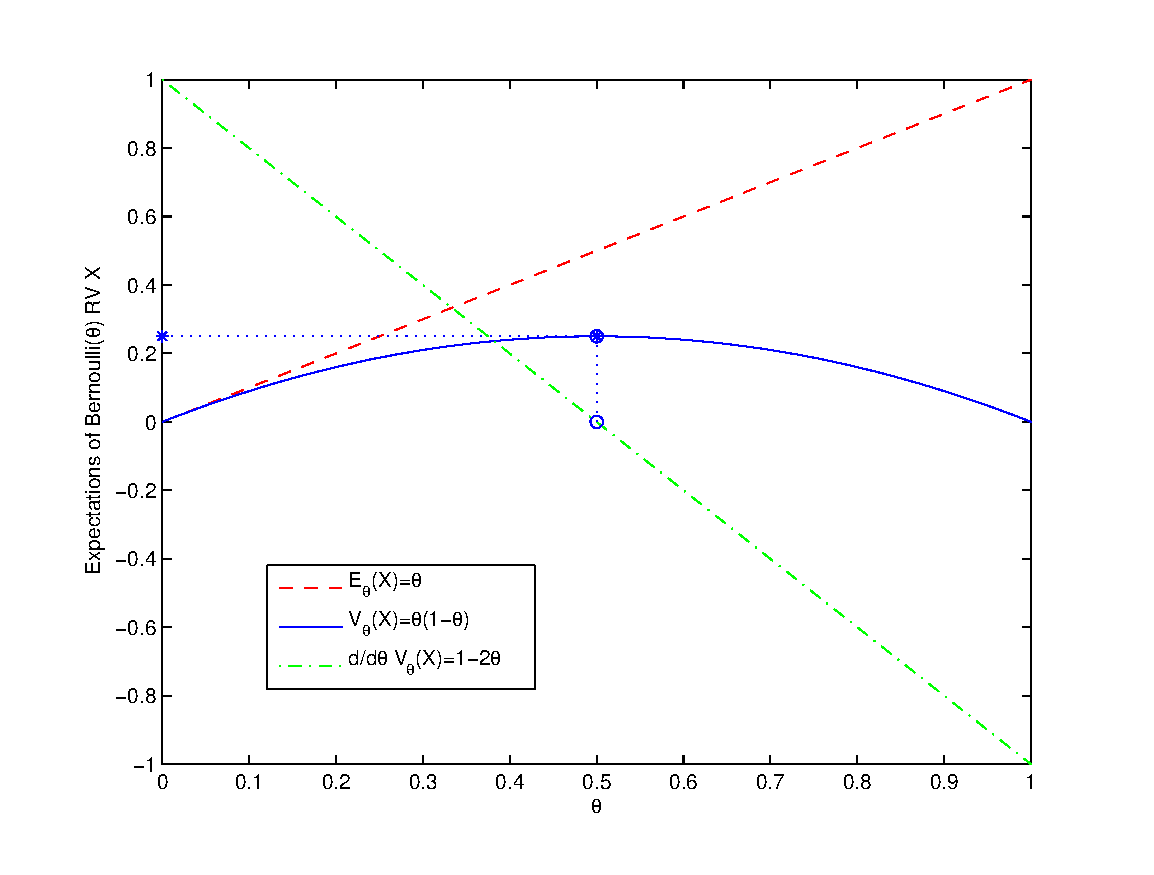
\includegraphics[width=5.0in]{figures/PlotMeanVarBernoulli}}
\end{figure}

Maximum of the variance $\V_{\theta}(X)$ is found by setting the derivative to zero, solving for $\theta$ and showing the second derivative is locally negative, i.e.~$\V_{\theta}(X)$ is concave down:
\[
\V_{\theta}'(X) := \frac{d}{d \theta} \V_{\theta}(X) = 1-2 \theta = 0  \iff \theta = \frac{1}{2} \ , 
\qquad \V_{\theta}''(X) := \frac{d}{d \theta} \left( \frac{d}{d \theta} \V_{\theta}(X) \right) = -2 < 0 \ ,
\]
\[
\max_{\theta \in [0,1]} \V_{\theta}(X) = \frac{1}{2} \left(1-\frac{1}{2} \right) = \frac{1}{4} \ , 
\text{since $\V_{\theta}(X)$ is maximized at $\theta = \frac{1}{2}$}
\]
The plot depicting these expectations as well as the rate of change of the variance are depicted in \hyperref[F:MeanVarBernoulli]{Figure \ref*{F:MeanVarBernoulli}}.  Note from this Figure that $\V_{\theta}(X)$ attains its maximum  value of $1/4$ at $\theta=0.5$ where $\frac{d}{d\theta}\V_{\theta}(X)=0$.  Furthermore, we know that we don't have a minimum at $\theta=0.5$ since the second derivative $\V_{\theta}''(X) = -2$ is negative for any $\theta \in [0,1]$.  This confirms that $\V_{\theta}(X)$ is concave down and therefore we have a maximum of $\V_{\theta}(X)$ at $\theta=0.5$.  We will revisit this example when we employ a numerical approach called Newton-Raphson method to solve for the maximum of a differentiable function by setting its derivative equal to zero.

\paragraph{Mean and variance of $\uniform(0,1)$ RV:}
Let $X \sim \uniform(0,1)$.  Then, 
\[
\e(X) = \int_{x=0}^1 x f(x)\, dx = \int_{x=0}^1 x \ 1 \, dx = \frac{1}{2} \left( x^2 \right]_{x=0}^{x=1} = \frac{1}{2} \left( 1-0 \right) = \frac{1}{2} \ ,
\]
\[
\e(X^2) = \int_{x=0}^1 x^2 f(x)\, dx = \int_{x=0}^1 x^2 \ 1 \, dx =  \frac{1}{3} \left( x^3 \right]_{x=0}^{x=1} = \frac{1}{3} \left( 1-0 \right) = \frac{1}{3} \ ,
\]
\[
\V(X) = \e(X^2) - (\e(X))^2 = \frac{1}{3}  - \left( \frac{1}{2} \right)^2  = \frac{1}{3}  - \frac{1}{4} = \frac{1}{12} \ .
\]

\begin{example}[Expected Exponential of the $Uniform(0,1)$ RV]
Let $X \sim Uniform(0,1)$ and $Y=r(X)=e^X$.  Compute $\e(Y)$. 

We can simply apply the definition of $\e(r(X))$, since $Y=r(X)$, is just a function of $X$, as follows: 
\[
\e(Y) = \int_0^1 e^x f(x) dx = \int_0^1 e^x 1 \ dx = e-1 \ .
\]
%You could have also found out that the density $f(y)=1/y$ for the RV $Y$, provided $1<y<e$, and $0$ otherwise.  Again,
%\[
%\e(Y) = \int_1^e y f(y) dy = \int_1^e y \frac{1}{y} dy = \int_1^e 1 \ dy = e-1 \ .
%\]
\end{example}

\paragraph{Mean and Variance of $\exponential(\lambda)$:}
Show that the mean of an $\exponential(\lambda)$ RV $X$ is:
\[
\e_{\lambda}(X) = \int_{0}^{\infty} x f(x;\lambda)\,dx
=   \int_{0}^{\infty} x \lambda e^{-\lambda x}\,dx
= \frac{1}{\lambda} \ ,
\]
and the variance is:
\[
\V_{\lambda}(X) = \left(  \frac{1}{\lambda} \right)^2 \ .
\]


\section{Stochastic Processes}\label{S:StochProc}

\begin{definition}[Stochastic Process]
A collection of RVs  \[
\left(X_{\alpha} \right)_{\alpha \in N} := \left( \  X_{\alpha} : \alpha \in \Az \  \right)
\]
is called a {\bf stochastic process}.  Thus, for every $\alpha \in  \Az$, the index set of the stochastic process, $X_{\alpha}$ is a RV.  If the index set $ \Az  \subset \Zz$ then we have  a {\bf discrete time stochastic process}, typically denoted by 
\[
\left(X_i\right)_{i \in \Zz} := \ldots, X_{-2},X_{-1},X_0, X_1,X_2,\ldots , \  \text{or}
\]
\[
\left( X_i \right)_{i \in \Nz} := X_1,X_2,\ldots , \  \text{or}
\]
\[
\left( X_i \right)_{i \in [n]} := X_1,X_2,\ldots , X_n , \ \text{where, } [n]:= \{1,2,\ldots,n\} \ .
\]
If $\Az \subset \Rz$ then we have a {\bf continuous time stochastic process}, typically denoted by $\{X_t\}_{t \in \Rz}$, etc.  
\end{definition}

Of course the above process is quite general and can allow for arbitrary dependence among the RVs.  
Generally, we cannot produce useful models without making simplifying assumptions. 
The absolutely simplest but extremely useful assumption is that of the {\bf Independent and Identically Distributed or IID Process} or merely {\bf IID Sequence of RVs} when the index set is a subset of $\Nz$. 

This is exactly rhe sequence of RVs associated with our product experiment $\mathcal{E}^{\otimes \infty} := (\Omega, \mathcal{F}_{\mathcal{X}}, P_{\theta})^{\otimes \infty}$.
    
\begin{definition}[Independent and Identically Distributed (IID) Process]
The finite or infinite sequence of RVs or the stochastic process $X_1, X_2,\ldots$ is said to be independent and identically distributed or IID if :
\begin{itemize}
\item they are an idependently distributed according to \hyperref[D:IndRVs]{Definition \ref*{D:IndRVs}}, and
\item $F(X_1) = F(X_2) = \cdots $, ie.~all the $X_i$'s have the same DF $F(X_1)$.
\end{itemize}
This is perhaps the most elementary class of stochastic processes and we succinctly denote it by
\[
\left(X_i\right)_{i \in [n]} := X_1, X_2,\ldots, X_n \overset{\IID}{\sim} F, \quad \text{or} \quad \left(X_i\right)_{i \in \Nz} := X_1, X_2,\ldots  \overset{\IID}{\sim} F \ .
\]
We sometimes replace the DF $F$ above by the name of the RV.
 \end{definition}
 
\begin{definition}[Independently Distributed]
The sequence of RVs or the stochastic process $\left(X_i\right)_{i \in \Nz} := X_1, X_2,\ldots$ is said to be independently distributed if :
\begin{itemize}
\item $X_1, X_2,\ldots$ is independently distributed according to \hyperref[D:IndRVs]{Definition \ref*{D:IndRVs}}.
\end{itemize}
This is a class of stochastic processes that is more general than the IID class.
\end{definition}

Let us consider a RV that arises from an IID stochastic process of $\bernoulli(\theta)$ RVs $\{X_i\}_{i \in \Nz}$, ie.~
\[
 \{X_i\}_{i \in \Nz} := \{X_1, X_2,\ldots\}  \overset{\IID}{\sim} \bernoulli(\theta) \ .
\]
When we consider the number of IID $\bernoulli(\theta)$ trials before the first `Head' occurs we get the following discrete RV.
\begin{model}[$\geometric(\theta)$ RV]
Given a parameter $\theta \in (0,1)$, the PMF of the $\geometric(\theta)$ RV $X$ is
\begin{equation}\label{E:Geometricpdf}
f(x;\theta) =
\begin{cases}
\theta(1-\theta)^{x} & \text{if $x \in \Zz_+ := \{0,1,2,\ldots \}$} \\
0 & \text{otherwise}
\end{cases}
\end{equation}
It is straightforward to verify that $f(x;\theta)$ is indeed a PDF :
\[
\sum_{x=0}^{\infty} f(x;\theta) = \sum_{x=0}^{\infty} \theta(1-\theta)^{x}
= \theta \left( \frac{1}{1-(1-\theta)} \right) =  \theta \left( \frac{1}{\theta} \right) = 1
\]

{\scriptsize
The above equality is a consequence of the geometric series identity \eqref{E:GeomSeries} with $a=\theta$ and $\vartheta:=1-\theta$:
\begin{equation}\label{E:GeomSeries}
 \sum_{ x =0}^{\infty} a \vartheta^x = a \left( \frac{1}{1-\vartheta} \right) , \ \text{provided, } 0 < \vartheta < 1 \ .
\end{equation}
\begin{proof}
\[
a+a\vartheta+a\vartheta^2+\cdots+a\vartheta^n
= \sum_{0 \leq x \leq n} a \vartheta^x
= a+ \sum_{1 \leq x \leq n} a \vartheta^x
= a +  \vartheta  \sum_{1 \leq x \leq n} a \vartheta^{x-1}
= a +  \vartheta  \sum_{0 \leq x \leq n-1} a \vartheta^{x}
= a +  \vartheta  \sum_{0 \leq x \leq n} a \vartheta^{x} - a \vartheta^{n+1}
\]
Therefore,
\begin{eqnarray}
\sum_{0 \leq x \leq n} a \vartheta^x
&=&  a +  \vartheta  \sum_{0 \leq x \leq n} a \vartheta^{x} - a \vartheta^{n+1} \notag \\
\left( \sum_{0 \leq x \leq n} a \vartheta^x \right) - \left( \vartheta  \sum_{0 \leq x \leq n} a \vartheta^{x} \right)
&=&  a  - a \vartheta^{n+1} \notag \\
\left( \sum_{0 \leq x \leq n} a \vartheta^x \right) (1-\vartheta)
&=&  a (1 -  \vartheta^{n+1}) \notag \\
\sum_{0 \leq x \leq n} a \vartheta^x
&=&  a \left( \frac{1 -  \vartheta^{n+1}}{1-\vartheta} \right) \notag\\
 \sum_{ x =0}^{\infty} a \vartheta^x  := \lim_{n \rightarrow \infty} \sum_{0 \leq x \leq n} a \vartheta^x
&=&  a \left( \frac{1}{1-\vartheta} \right) , \ \text{provided, } 0 < \vartheta < 1 \notag
\end{eqnarray}
\end{proof}
}
The outcome of a $\geometric(\theta)$ RV can be thought of as ``the number of tosses needed before the appearance of the first `Head' when tossing a coin with probability of `Heads' equal to $\theta$ in a independent and identical manner.''
\end{model}

\begin{figure}[htpb]
\caption{PDF of $X \sim \geometric(\theta=0.5)$ and the relative frequency histogram based on $100$ and $1000$ samples from $X$ according to Simulation~\ref{SIM:Geometric} and Labwork~\ref{LW:RelFreqHistForGeomSims}.\label{F:PlotPdfSimHistGeomthetaHalf}}
\centering   \makebox{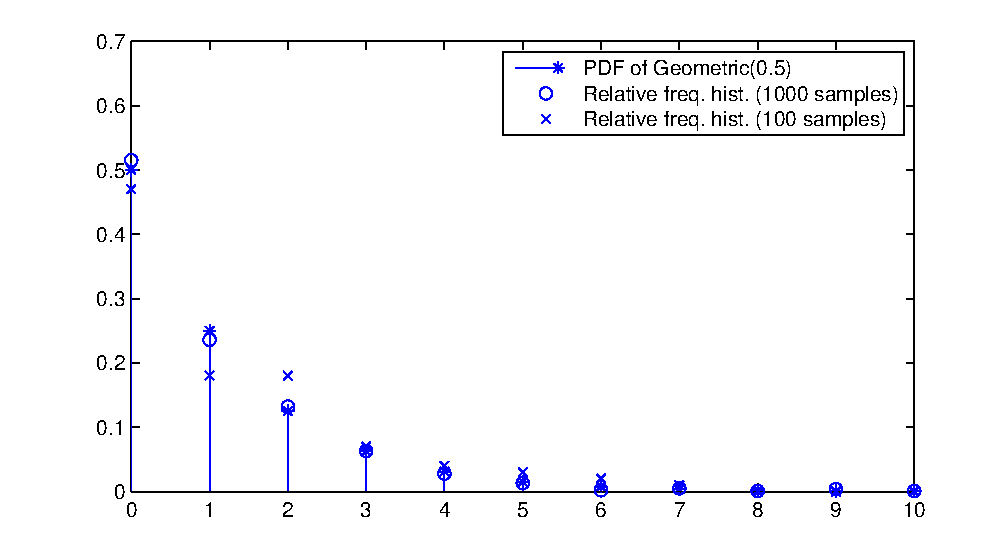
\includegraphics[width=6.50in]{figures/PlotPdfSimHistGeomthetaHalf}}
\end{figure}

\paragraph{Mean and variance of $\geometric(\theta)$ RV:}
Let $X \sim \geometric(\theta)$ RV.  Then,
\[
\e(X) = \sum_{x=0}^{\infty} x \theta(1-\theta)^x =  \theta \sum_{x=0}^{\infty} x (1-\theta)^x
\]
In order to simplify the RHS above, let us employ differentiation with respect to $\theta$:
\[
\frac{-1}{\theta^2}= \frac{d}{d\theta} \left( \frac{1}{\theta} \right)= \frac{d}{d\theta} \sum_{x=0}^{\infty} (1-\theta)^x  =  \sum_{x=0}^{\infty} -x (1-\theta)^{x-1}
\]
Multiplying the LHS and RHS above by $-(1-\theta)$ and substituting in $\e(X)=  \theta \sum_{x=0}^{\infty} x (1-\theta)^x$, we get a much simpler expression for $\e(X)$ :
\[
\frac{1-\theta}{\theta^2}= \sum_{x=0}^{\infty} x (1-\theta)^{x} \implies \e(X) = \theta \left( \frac{1-\theta}{\theta^2} \right) = \frac{1-\theta}{\theta} \ .
\]
Similarly, it can be shown that
\[
\V(X) = \frac{1-\theta}{\theta^2} \ .
\]

\begin{figure}[htpb]
\caption{Mean and variance of a $\geometric(\theta)$ RV $X$ as a function of the parameter $\theta$.\label{F:MeanVarGeom}}
\centering   \makebox{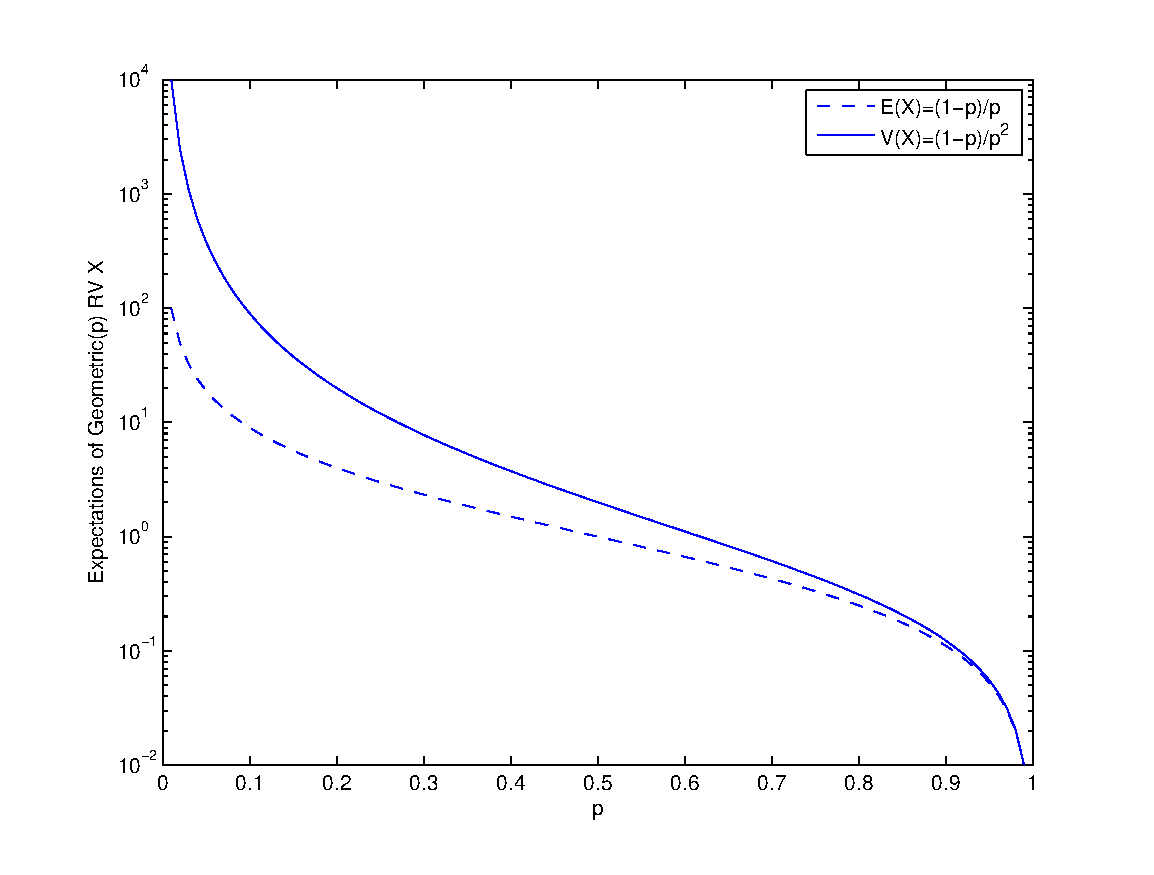
\includegraphics[width=5.0in]{figures/PlotMeanVarGeom}}
\end{figure}

\begin{example}[Coupon Collectors Problem]
Recall the Coupon Collector's Probelms from lectures.%TODO
\vspace{5cm}
~ 
\end{example}

The RV $Y$ in \hyperref[T:T3XRVs]{Table \ref*{T:T3XRVs}} may be generalized to an experiment $\E{E}_{\theta}^{n}$ with $n$ coin tosses.  
%}% end remove
Let $X_i$ be the Indicator function of the event `Heads on the $i$-th toss' as before.  Then $Y$ defined by,
 \[
 Y := \sum_{i=1}^n X_i := X_1 + X_2 + \cdots + X_n  \ ,
 \]
is the number of `Heads' in $n$ tosses.  
%\remove{
Akin to the second row of \hyperref[T:T3XRVs]{Table \ref*{T:T3XRVs}}, for the `Toss $n$ times' experiment $\E{E}_{\theta}^{n}$ the
%} 
RV $Y$ as defined above will take values in $\{0,1,2,\ldots,n\}$ and is therefore a discrete RV.  This is called the Binomial RV as defined next.  
%\remove{
But, first we remind ourselves of some elementary definitions involving arrangements of objects from a collection (recall \hyperref[S:PermsFactsCombs]{Section~\ref*{S:PermsFactsCombs}}).
%}%end remove

\begin{model}[$\binomial(n,\theta)$ RV]\label{M:binomial}
Let the RV $X=\sum_{i=1}^n X_i$ be the sum of $n$ independent and identically distributed $\bernoulli(\theta)$ RVs, i.e.:
\[
X=\sum_{i=1}^n X_i, \qquad X_1,X_2,\ldots,X_n \overset{\IID}{\sim} \bernoulli(\theta) \ .
\]
Given two parameters $n$ and $\theta$, the PMF of the $\binomial(n,\theta)$ RV $X$ is:
\begin{equation}
 f(x; n,\theta) =
 \begin{cases}
 \displaystyle\binom{n}{x} \theta^x (1-\theta)^{n-x} & \text{if $x \in \{0,1,2,3,\ldots,n\}$} \ ,\\
 0 & \text{otherwise}
 \end{cases}
 \end{equation}
where, $\binom{n}{x}$ is:
\[
\binom{n}{x} = \frac{n(n-1)(n-2)\ldots(n-x+1)}{x(x-1)(x-2)\cdots (2)(1)} =  \frac{n !}{x! (n-x)!} \ .
 \]
$\binom{n}{x}$ is read as ``$n$ choose $x$.''
 \end{model}
 %{\scriptsize
\begin{proof} This is only a sketch. A formal proof should start with the mathematical induction for the very formula for the binomial coeeficient.

Observe that for the $\binomial(n,\theta)$ RV $X$, $\p(X=x) = f(x;n,\theta)$ is the probability that $x$ of the $n$ $\bernoulli(\theta)$ trials result in an outcome of $1$'s.  Next note that if all $n$ $X_i$'s are $0$'s, then $X=0$, and if all $n$ $X_i$'s are $1$'s, then $X=n$.  In general, if some of the $n$ $X_i$'s are $1$'s and the others are $0$, then $X$ can only take values in $\{0,1,2,\ldots,n\}$ and therefore $f(x;n,\theta)=0$ if $x \notin \{0,1,2,\ldots,n\}$.

Now, let us compute $f(x;n,\theta)$ when $x\in\{0,1,2,\ldots,n\}$.  Consider the set of indices $\{1,2,3,\ldots,n\}$ for the $n$ IID $\bernoulli(\theta)$ RVs $\{X_1,X_2,\ldots,X_n\}$.  Now choose $x$ indices from $\{1,2,\ldots,n\}$ to mark those trials in a particular realization of $\{x_1,x_2,\ldots,x_n\}$ with the Bernoulli outcome of $1$.  The probability of each such event is $\theta^x (1-\theta)^{n-x}$ due to the IID assumption.  For each realization $\{x_1,x_2,\ldots,x_n\} \in \{0,1\}^{n} := \{ \text{all binary $(0-1)$ strings of length $n$}\}$, specified by a choice of $x$ trial indices with Bernoulli outcome $1$, the binomial RV $X=\sum_{i=1}^n X_i$ takes the value $x$.  Since there are exactly $\binom{n}{x}$ many ways in which we can choose $x$ trial indices (with outcome $1$) from the set of $n$ trial indices $\{1,2,\ldots,n\}$, we get the desired product for $f(x; n,\theta) = \binom{n}{x} \theta^x (1-\theta)^{n-x}$ when $x \in \{0,1,\ldots,n\}$.
\end{proof}
%}
\paragraph{Mean and variance of $\binomial(n,\theta)$ RV:}
Let $X \sim \binomial(n,\theta)$.  Based on the definition of expectation:
\[
\e(X) = \int x \, dF(x; n,\theta) = \sum_x x f(x;n,\theta) = \sum_{x =0}^n x \binom{n}{x} \theta^x (1-\theta)^{n-x} \ .
\]
However, this is a nontrivial sum to evaluate.  Instead, we may use \eqref{E:EofLinCombofRVs} and \eqref{E:VofLinCombofRVs} by noting that $X = \sum_{i=1}^n X_i$, where the $\{X_1,X_2,\ldots,X_n \} \overset{\IID}{\sim} \bernoulli(\theta)$, $\e(X_i) = \theta$ and $\V(X_i)=\theta(1-\theta)$:
\[
\e(X) = \e(X_1+X_2, \cdots ,X_n) = \e \left( \sum_{i=1}^n X_i \right) = \sum_{i=1}^n \e(X_i) = n \theta \ ,
\]
\[
\V(X) = \V \left( \sum_{i=1}^n X_i \right) = \sum_{i=1}^n \V(X_i) = \sum_{i=1}^n{\theta(1-\theta)} = n\theta(1-\theta) \ .
\]

\begin{figure}[htpb]
\caption{PDF of $X \sim \binomial(n=10,\theta=0.5)$ and the relative frequency histogram based on $100,000$ samples from $X$ obtained according to Simulation~\ref{SIM:BinomialFromGeoms}.\label{F:PlotPdfSim10000HistBinomByGeomsn10thetaHalf}} % TODO check which of two simulation algs is coming from
\centering   \makebox{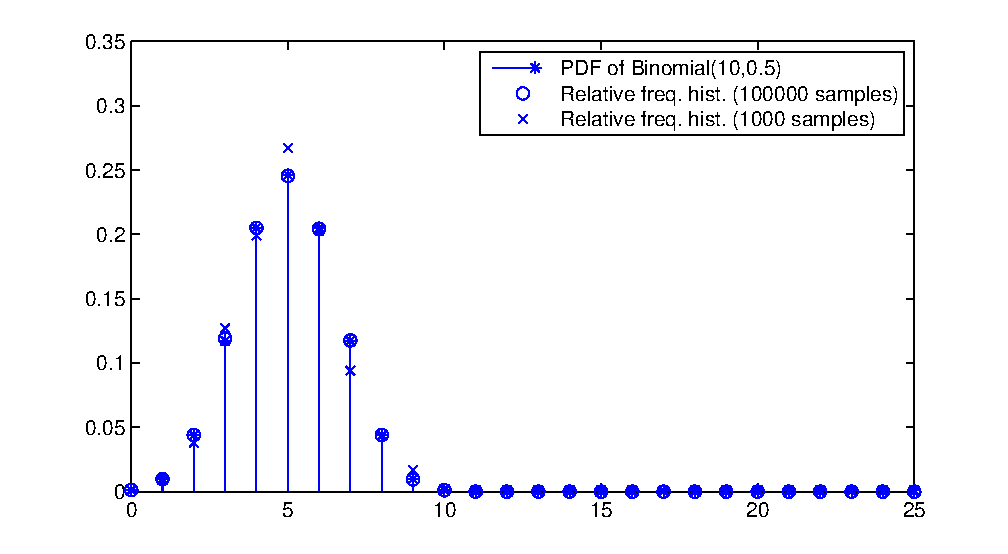
\includegraphics[width=6.50in]{figures/PlotPdfSim10000HistBinomByGeomsn10thetaHalf}}
\end{figure}


In several situations it becomes cumbersome to model the events using the $\binomial(n,\theta)$ RV, especially when when the parameter $\theta \propto 1/n$ and the events become rare.  However, for some real parameter $\lambda>0$, the $\binomial(n,\lambda/n)$ RV with probability of the number of successes in $n$ trials, with per-trial success probability $\lambda/n$, approaches the Poisson distribution with expectation $\lambda$, as $n$ approaches $\infty$ (actually, it converges in distribution as defined later).  The $\poisson(\lambda)$ RV is much simpler to work with than the combinatorially laden $\binomial(n,\theta=\lambda/n)$ RV.  We sketch the details of this next.

%{\scriptsize
Let $X \sim \binomial(n,\theta=\lambda/n)$, then for any $x \in \{0,1,2,3,\ldots,n\}$,
\begin{eqnarray}
\p(X=x)
&=&
\binom{n}{x} \left( \frac{\lambda}{n} \right)^x \left( 1- \frac{\lambda}{n} \right)^{n-x} \notag \\
&=& \frac{n(n-1)(n-2)\cdots(n-x+1)}{x(x-1)(x-2)\cdots (2)(1)}
\left( \frac{\lambda^x}{n^x} \right)
\left( 1- \frac{\lambda}{n} \right)^n
\left( 1- \frac{\lambda}{n} \right)^{-x} \notag \\
&=&
\overbrace{\left( \frac{n}{n} \right) \left( \frac{n-1}{n} \right) \left( \frac{n-2}{n} \right) \cdots \left( \frac{n-x+1}{n} \right)}
\overbrace{\left( \frac{\lambda^x}{x!} \right)}
\underbrace{\left( 1- \frac{\lambda}{n} \right)^n}
\underbrace{\left( 1- \frac{\lambda}{n} \right)^{-x}}  \notag \\
\end{eqnarray}

As $n \to \infty$, the expression below the first overbrace $\to 1$, while that below the second overbrace, being independent of $n$ remains the same.  By the elementary examples of limits
%\remove{
\ref*{EX:LimitExpofLambda} and \ref*{EX:Limit1MinusLambdaOverNToMinusK}%}
, as $n \to \infty$, the expression over the first underbrace approaches $e^{-\lambda}$ while that over the second underbrace approaches $1$.  Finally, we get the desired limit:

\[
\lim_{n \to \infty} \p(X=x)
= \frac{ e^{-\lambda} \lambda^x}{x!}  \ .
\]
%}
\begin{model}[$\poisson(\lambda)$ RV]\label{M:Poisson}
Given a real parameter $\lambda>0$, the discrete RV $X$ is said to be $\poisson(\lambda)$ distributed if $X$ has PDF:
\begin{equation}\label{E:Poissonpdf}
f(x;\lambda) =
\begin{cases}
 \frac{ e^{-\lambda} \lambda^x}{x!} & \text{if $x \in \Zz_+ := \{0,1,2,\ldots\}$} \ , \\
0 & \text{otherwise} \ .
\end{cases}
\end{equation}

Note that the PDF integrates to $1$:
\[
\sum_{x=0}^{\infty} f(x;\lambda)
= \sum_{x=0}^{\infty}  \frac{ e^{-\lambda} \lambda^x}{x!}
=  e^{-\lambda} \sum_{x=0}^{\infty}  \frac{\lambda^x}{x!}
=  e^{-\lambda} e^{\lambda}
= 1 \ ,
\]
where we exploit the Taylor series of $e^{\lambda}$ to obtain the second-last equality above.
\end{model}

\paragraph{Mean and variance of $\poisson(\lambda)$ RV:}
Let $X \sim \poisson(\lambda)$.  Then:
\[
\e(X) = \sum_{x=0}^{\infty} x f(x;\lambda)
= \sum_{x =0}^{\infty} x \frac{ e^{-\lambda} \lambda^x}{x!}
= e^{-\lambda} \sum_{x =0}^{\infty} x \frac{  \lambda^x}{x!}
= e^{-\lambda} \sum_{x -1 =0}^{\infty} \frac{ \lambda \lambda^{x-1}}{(x-1)!}
= e^{-\lambda} \lambda e^{\lambda}
= \lambda
\ .
\]
Similarly,
\[
\V(X) = \e(X^2)-(\e(X))^2 = \lambda + \lambda^2 - \lambda^2 = \lambda \ .
\]
since
\begin{align*}
\e(X^2)& = \sum_{x=0}^{\infty} x^2 \frac{e^{-\lambda} \lambda^x}{x!} = \lambda \, e^{-\lambda} \sum_{x=1}^{\infty} \frac{x \, \lambda^{x-1}}{(x-1)!}
= \lambda \, e^{-\lambda} \left( 1 + \frac{2 \lambda}{1} + \frac{3 \lambda^2}{2!} + \frac{4 \lambda^3}{3!} + ... \right)\\
&= \lambda \, e^{-\lambda} \left( \left( 1 + \frac{\lambda}{1} + \frac{\lambda^2}{2!} + \frac{\lambda^3}{3!} + ... \right) + \left[ \frac{\lambda}{1} + \frac{2 \lambda^2}{2!} + \frac{3 \lambda^3}{3!} + ... \right] \right)\\
&= \lambda \, e^{-\lambda} \left( \left( e^{\lambda} \right) + \lambda \left( 1 + \frac{2 \lambda}{2!} + \frac{3 \lambda^2}{3!} + ... \right) \right)
= \lambda \, e^{-\lambda} \left( e^{\lambda} + \lambda \left( 1 + \lambda + \frac{\lambda^2}{2!} + ... \right) \right)\\
&= \lambda \, e^{-\lambda} \left( e^{\lambda} + \lambda \left( e^{\lambda} \right) \right)
= \lambda \, e^{-\lambda} \left( e^{\lambda} + \lambda\, e^{\lambda}\right) = \lambda (1 + \lambda) = \lambda + \lambda^2
\end{align*}

Note that $\poisson(\lambda)$ distribution is one whose mean and variance are the same, namely $\lambda$.

%\remove{
\begin{figure}[htpb]
\caption{PDF of $X \sim \poisson(\lambda=10)$ and the relative frequency histogram based on 1000 samples from $X$ according to Simulation~\ref{SIM:Poisson}.\label{F:PlotPdfSim1000HistPoiss10}}
\centering   \makebox{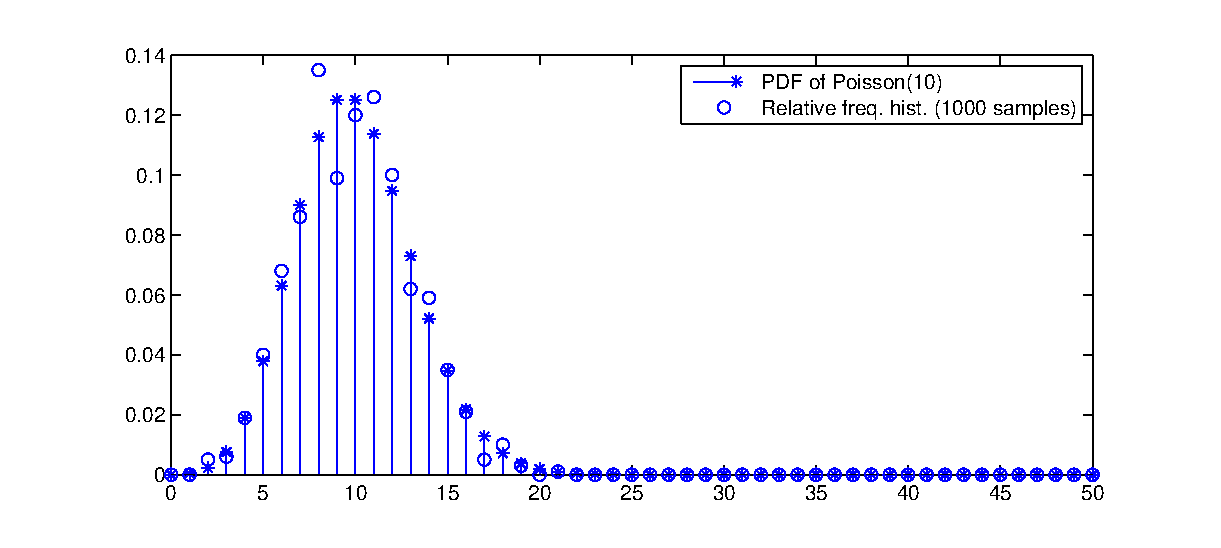
\includegraphics[width=6.50in]{figures/PlotPdfSim1000HistPoiss10}}
\end{figure}
%}%end remove

The $\poisson(\lambda)$ RV $X$ is also related to the IID $\exponential(\lambda)$ RV $Y_1,Y_2,\ldots$: $X$ is the number of occurrences, per unit time, of an instantaneous event whose inter-occurrence time is the IID $\exponential(\lambda)$ RV.  For example, the number of buses arriving at our bus-stop in the next minute, with exponentially distributed inter-arrival times, has a Poisson distribution.

\newpage
\section*{Exercises}

\begin{ExerciseList}
\Exercise
One number in the following table for the probability function of a random variable $X$ is incorrect.  
Which is it, and what should the correct value be?
$$
\begin{array}{c|ccccc}
x&1&2&3&4&5\\\hline
\p(X=x)&0.07&0.10&1.10&0.32&0.40
\end{array}
$$
\Answer
$\p(X=3)$ does not satisfy the condition that $0\leq \p(A)\leq1$ for any event $A$.  
If $\Omega$ is the sample space, then $\p(\Omega)=1$ and so  the correct probability is 
\[
\p(X=3)\;=\;1-0.07-0.10-0.32-0.40\;=\;0.11 \enspace .
\]

\Exercise
Let $X$ be the number of years before a particular type of machine will need replacement.  
Assume that $X$ has the probability function $f(1)=0.1$, $f(2)=0.2$, $f(3)=0.2$, $f(4)=0.2$, $f(5)=0.3$.
\be
\item Find the distribution
  function, $F$,  for $X$, and graph both $f$ and $F$.

\item  Find the probability that the machine needs to be
  replaced during the first 3 years.

\item  Find the probability that the machine needs no
  replacement during the first 3 years.
\ee
\Answer
\be
\item  Tabulate the values for the probability mass function  as follows: $$
\begin{array}{c|ccccc}
x&1&2&3&4&5\\\hline
\p(X=x)&0.1&0.2&0.2&0.2&0.3
\end{array}
$$so the  distribution function is:
\[F(x)\; = \;\p(X \leq x) \;=\;
\begin{cases}
 0 & \text{ if }  0 \leq   x < 1\\
 0.1 & \text{ if } 1 \leq  x < 2\\
0.3 & \text{ if } 2 \leq x < 3\\
 0.5 & \text{ if } 3 \leq x < 4\\
0.7 & \text{ if }  4 \leq x < 5\\
 1& \text{ if }    x \geq 5
\end{cases}
\]

The graphs of $f(x)$ and $F(x)$ for random variable $X$ are shown below:

%TODO\centering   \makebox{\includegraphics[width=6.5in]{figures/fandFfor5YearMachine.png}}



\item The probability that the machine needs to be replaced during the
  first 3 years is:
$$\p(X \leq  3)\;=\;\p(X=1)+\p(X=2)+\p(X=3)\;=\;0.1+0.2+0.2\;=\;0.5\,.$$
(This answer is easily seen  from the distribution function of $X$.)
\item The probability that the machine needs no replacement during the
first three years is
\[ \p(X >  3)\;=\;\, 1-\p(X \leq  3)\,=\, 0.5 \,.\]
\ee

\Exercise
Of 200 adults, 176 own one TV set, 22 own two TV sets, and 2 own three TV sets.  
A person is chosen at random. What is the probability mass function of $X$,  the number of TV sets owned by that person?
\Answer
Assuming that the probability model is being built from the observed relative frequencies, the probability mass function is:
$$
f(x)\;=\;\begin{cases}\frac{176}{200}&x=1\\\frac{22}{200}&x=2\\\frac{2}{200}&x=3\end{cases}$$

\Exercise
Suppose a discrete random variable $X$ has probability function give by
$$\begin{array}{c|cccccccccccc}
x&3&4&5&6&7&8&9&10&11&12&13\\\hline
 \p(X=x)&0.07&0.01&0.09&0.01&0.16&0.25&0.20&0.03&0.02&0.11&0.05
\end{array}
$$
\be
\item[(a)] Construct a row of cumulative probabilities for this table, that
  is, find the distribution function of $X$.
\item[(b)] Find  the following  probabilities.
\bcols{3}
\be
\item[(i)]$\p(X\leq 5)$
\item[(ii)] $\p(X<12)$
\item[(iii)] $\p(X>9)$
\item[(iv)] $\p(X\geq 9)$
\item[(v)] $\p(4 <  X\leq 9)$
\item[(vi)] $\p(4<X<11)$
\ee
\ecols
\ee

\Answer
\begin{itemize}
\item[(a)]  $$\begin{array}{c|cccccccccccc}
x&3&4&5&6&7&8&9&10&11&12&13\\\hline
F(x) =\p(X\leq x)&0.07&0.08&0.17&0.18&0.34&0.59&0.79&0.82&0.84&0.95&1.00
\end{array}
$$

\medskip
\item[(b)]
\be
\item[(i)]$\p(X\leq 5)= F(5) = 0.17$ \\[3pt]
\item[(ii)]$\p(X<12)=\p(X\leq11) = F(11) =0.84$\\[3pt]
\item[(iii)] $\p(X>9)= 1 - \p(X\leq 9) = 1- F(9) =1-0.79=0.21$ \\[3pt]
\item[(iv)] $\p(X\geq 9)=1-\p(X <  9)=1-\p(X\leq 8)=1-0.59=0.41$ \\[3pt]
\item[(v)] $\p(4 <  X\leq 9)= F(9) - F(4) =0.79-0.08=0.71$ \\[3pt]
\item[(vi)] $\p(4<X<11)=\p(4 <  X\leq 10)= F(10) -F(4) =0.82- 0.08=0.74$ \\[3pt]
\ee
\end{itemize}


\Exercise
A box contains 4 right-handed and 6 left-handed screws.  
Two screws are drawn at random without replacement. Let $X$ be the number of left-handed screws drawn.  
Find the probability mass function for $X$, and then calculate  the following probabilities:
\be
\item $\p(X\leq 1)$
\item $\p(X\geq 1)$
\item $\p(X>1)$
\ee
\Answer
Since  we are sampling without replacement,
\begin{eqnarray*}
\p(X=0) &=& \frac{4}{10}\cdot\frac{3}{9} = \frac{2}{15}\quad (\text{one way of drawing two right screws}), \\
\p(X=1) &=& \frac{6}{10}\cdot\frac{4}{9}+\frac{4}{10}\cdot\frac{6}{9} = \frac{8}{15}\quad(\text{two ways of drawing one left and one  right screw}),\\
\p(X=2) &=& \frac{6}{10}\cdot\frac{5}{9} = \frac{1}{3}\quad(\text{one way of drawing two left screws}).
\end{eqnarray*}
So the probability mass function of $X$ is:
\[f(x)\;=\;\p(X=x)\;=\;
\begin{cases}
\frac{2}{15}  & \text{if } x=0\\[3pt]
\frac{8}{15} & \text{if } x=1\\[3pt]
\frac{1}{3}  & \text{if } x=2
\end{cases}\]

The required probabilities are:
\be
\item
$$\p(X\leq1)\;=\;\p(X=0)+\p(X=1)\;=\;\frac{2}{15}+\frac{8}{15}\;=\;\frac{2}{3}$$
\item
$$\p(X\geq 1)\;=\;\p(X=1)+\p(X=2)\;=\;\frac{8}{15}+\frac{1}{3}\;=\;\frac{13}{15}$$
\item
$$\p(X>1)\;=\;\p(X=2)\;=\;\frac{1}{3}$$
\ee

\Exercise
Suppose that  a random variable $X$ has geometric  probability mass function,
  \[f(x)\;=\;\frac{k}{2^x}\quad (x=0,1,2,\dots)\,.\]
\be
\item Find the value of  $k$.
\item  What is  $\p(X\geq 4)$?
\ee
\Answer
\be
\item
Since $f$ is a probability mass function,  $$\sum_{x=0}^\infty\frac{k}{2^x}\;=\;1\,, 
\qquad \text{that is,}\qquad k\,\sum_{x=0}^\infty\frac{1}{2^x}\;=\;1\ \enspace.$$
Now $\displaystyle \sum_{x=0}^\infty\frac{1}{2^x}$ is a geometric series with common ratio $r= \frac{1}{2}$ and first term $a=1$,
and so has  sum
\[ S\;=\; \frac{a}{1-r} \;=\;\frac{1}{1-\frac{1}{2} } \;=\; 2\]
Therefore, \[  2 k\;=\; 1 \,, \quad \text{that
  is,}\quad k\;=\; \frac{1}{2}\,.\]

\item From (a), the probability mass function of $f$ is
  $$f(x)\;=\;\frac{\frac{1}{2}}{2^{x}}\;=\;\frac{1}{2^{x+1}}\,.\quad
  (x=0,1,2,\dots)$$ Now
\[\p(X\geq 4)\;=\;1-\p(X<4)\;=\;1-\p(X\leq3)\] where
\ba{\p(X\leq3)&=\;\sum^3_{x=0}\frac{1}{2^{x+1}}\\[3pt]
&=\;\frac{1}{2}+\frac{1}{4}+\frac{1}{8}+\frac{1}{16}\\[3pt]
&=\;\frac{8}{16}+\frac{4}{16}+\frac{2}{16}+\frac{1}{16}\\[3pt]
&=\;\frac{15}{16}\enspace.
}
That is,  $\p(X\geq4)\,=\,\displaystyle \frac{1}{16}$.
\ee

\Exercise
Four fair coins are tossed simultaneously.  
If we count the number of heads that appear then we have a  binomial random variable,  $X=$ {\it the number of heads}.
\be
\item Find the probability mass
  function of  $X$.
\item  Compute the probabilities of obtaining no heads, precisely 1
  head, at least 1 head, not more than 3 heads.
\ee
\Answer
Note that  $\theta=\frac{1}{2}$ here.
\be
\item $X$ has probability mass function
\[f(x)\;=\;\begin{cases}
\displaystyle\displaystyle \binom{4}{0}\frac{1}{2}^0\frac{1}{2}^4=\frac{1}{16}&x=0\\[16pt]
\displaystyle\displaystyle\binom{4}{1}\frac{1}{2}^1\frac{1}{2}^3=\frac{4}{16}&x=1\\[16pt]
\displaystyle\displaystyle\binom{4}{2}\frac{1}{2}^2\frac{1}{2}^2=\frac{6}{16}&x=2\\[16pt]
\displaystyle\binom{4}{3}\frac{1}{2}^3\frac{1}{2}^1=\frac{4}{16}&x=3\\[16pt]
\displaystyle\binom{4}{4}\frac{1}{2}^4\frac{1}{2}^0=\frac{1}{16}&x=4
\displaystyle\end{cases}
\]

\item The required probabilities are:

$\displaystyle \p(X=0)=f(0)=\frac{1}{16}$\\[3pt]
$\displaystyle \p(X=1)=f(1)=\frac{4}{16}$\\[3pt]
$\displaystyle \p(X\geq1)=1-\p(X=0)=1-f(0)=\frac{15}{16}$\\[3pt]
$\displaystyle \p(X\leq3)=f(0)+f(1)+f(2)+f(3)=\frac{15}{16}$
\ee

\Exercise
The distribution of blood types in a certain  population is as follows:
$$
\begin{array}{c|cccc}
\text{Blood type}&\text{Type } O&\text{Type } A&\text{Type } B& \text{Type }AB\\\hline
\text{Proportion}&0.45&0.40&0.10&0.05
\end{array}
$$
A random sample of 15 blood donors is observed from this
population. Find the probabilities of the following events.

\be
\item Only one type $AB$ donor is included.
\item At least three of the donors are type $B$.
\item More than ten of the donors are \emph{either} type $O$ \emph{or} type $A$.
\item Fewer that five of the donors are \emph{not} type $A$.
\ee
\Answer
\be
\item  If the random variable $X$ denotes the number of type $AB$ blood donors
  in the sample of 15, then $X$ has a binomial distribution with $n=15$
  and $\theta=0.05$.  Therefore
\[\p(X=1) \;=\;\binom{15}{1} (0.05)^1  (0.95)^{14}\;=\;0.366 \quad (\text{3 sig. fig.}) \,.\]

\medskip
\item  If the random variable $X$ denotes the number of type $B$  blood donors
  in the sample of 15, then $X$ has a binomial distribution with $n=15$
  and $\theta=0.10$.  Therefore
\ba{\p(X\geq 3) &\;=\;  1\, - \,\p(X=0)\, -\, \p(X=1)\, -\, \p(X=2) \\[3pt]
 &\;=\;  1\; - \; \binom{15}{0} (0.1)^0  (0.9)^{15}\;-\; \binom{15}{1}
 (0.1)^1  (0.9)^{14}\;-\; \binom{15}{2} (0.1)^2  (0.9)^{13}\\[3pt]
&\;=\;  1\,-\, 0.2059 \,-\, 0.3432 \,-\, 0.2669\\[3pt]
&\;=  \;0.184 \quad (\text{to 3 sig. fig.})
}

\medskip
\item If the random variable $X$ denotes the number of type  $O$ or type $A$ blood donors
  in the sample of 15, then $X$ has a binomial distribution with $n=15$
  and $\theta=0.85$.  Therefore
\ba{\p(X > 10 ) &\;=\;  \p(X=11)\, + \, \p(X=12)\, +\,  \p(X=13) \, + \, \p(X=14)\, + \, \p(X=15)  \\[3pt]
 &\;=\;   \binom{15}{11} (0.85)^{11}  (0.15)^{4}\;+\; \binom{15}{12}
 (0.85)^{12}  (0.15)^{3}\\[3pt]
&\;+\; \binom{15}{13} (0.85)^{13}  (0.15)^{2}\;+\; \binom{15}{14} (0.85)^{14}  (0.15)^{1}\;+\; \binom{15}{15} (0.85)^{15}  (0.15)^{0}\\[3pt]
&\;=\;  0.1156 \,+\,0.2184 \,+\,0.2856 \,+\, 0.2312\,+\,0.0874\\[3pt]
&\;=\;0.938 \quad (\text{to 3 sig. fig.})
}

\medskip
\item If the random variable $X$ denotes the number of blood donors that
  are \emph{not} of type $A$ blood donors
  in the sample of 15, then $X$ has a binomial distribution with $n=15$
  and $\theta=0.6$.  Therefore
\ba{\p(X <  5) &\;=\;  \p(X=0)\, +\, \p(X=1)\, + \, \p(X=2)\, + \, \p(X=3)\, + \, \p(X=4) \\[3pt]
 &\;=\;   \binom{15}{0} (0.6)^0  (0.4)^{15}\;+\; \binom{15}{1}
 (0.6)^1  (0.4)^{14}\;+\; \binom{15}{2} (0.6)^2  (0.4)^{13}\\[3pt]
&\;+\; \binom{15}{3} (0.6)^3  (0.4)^{12}\;+\; \binom{15}{4} (0.6)^4  (0.4)^{11}\\[3pt]
&\;=\;  0.0000 \,+\,  0.0000\,+\, 0.0003\,+\, 0.0016\,+\,0.0074\\[3pt]
&\;=\;0.009 \quad (\text{to 3 DP.})
}
\ee



\Exercise
If the probability of hitting a target in a single shot is $10\%$ and 10 shots are fired independently, what is the probability that the target will be hit at least once?
\Answer
This is a Binomial experiment with parameters $\theta=0.1$ and $n=10$, and so 
\[\p(X\geq 1) = 1-\p(X<1) = 1-\p(X=0) \enspace ,\] 
where
\[\p(X=0) = \binom{10}{0}0.1^0 0.9^{10} \approxeq 0.3487 \enspace .\]

 Therefore, the probability that the target will be hit at least once is
 \[1- 0.3487 \approxeq 0.6513 \enspace .\]

\Exercise
Consider the probability density function
$$f(x)\;=\;\begin{cases} k &-4 \leq x\leq4\\0&\textrm{otherwise}\end{cases}\,.$$

\be
\item Find  the value of $k$.
\item Find the distribution function, $F$.
\item   Graph $f$ and  $F$.
\ee
\Answer
\be
\item Since $f(x)$ is a (continuous) probability density function which integrates to one,
$$\int_{-4}^4kdx\;=\;1\,.$$
That is, 
\ba{k \,x\bigg]^4_{-4}&=\;1\\[3pt]k(4-(-4))&=\;1\\[3pt]8k&=\;1\\[3pt]k&=\;\frac{1}{8}}

\item First note that if $x <  -4$, then  $$F(x)\;=\;\int^x_{-\infty}0\,dv\;=\;0\,.$$
If $-4 \leq x \leq 4$, then
\begin{align*}F(x)&=\;\int^{-4}_{-\infty}0\,dv\;+\;\int^x_{-4} \frac{1}{8}\,dv\\[3pt]
&=\;0\;+\;\left[ \frac{1}{8}\, v \right]^x_{-4}\\[3pt]
&=\;  \frac{1}{8} (x +4)\end{align*}
If $x\geq 4$, then
\begin{align*}F(x)&=\int^{-4}_{-\infty}0\,dv\;+\;\int^{4}_{-4}
  \frac{1}{8} \,dv\;+\;\int^x_{4} 0 \,dv\\[3pt]
&=0\;+\;\left[\frac{1}{8} v \right]^4_{-4}\;+\;0\\[3pt]
&=\; 1\end{align*}
Hence  $$F(x)\;=\;\begin{cases}0&x <  -4\\ \frac{1}{8} (x+4) &-4 \leq
  x\leq 4\\1&x\geq 4\end{cases}$$

\item  The graphs of $f(x)$ and $F(x)$ for  random variable $X$ are as follows:
%TODO\centering   \makebox{\includegraphics[width=6.5in]{figures/fandFforConstantDensity.png}}

\ee

\Exercise
Assume that a new light bulb will burn out at time $t$ hours according to the probability density function given by 
$$
f(t)\;=\;
\begin{cases}
\lambda e^{-\lambda t} & \text{ if } t >0 \enspace,\\
0 & \text{ otherwise} \enspace .
\end{cases}
$$
In this context, $\lambda$ is often called the failure rate of the bulb.

\be
\item[(a)]Assume that $\lambda=0.01$, and find the probability that the
  bulb will not burn out before $\tau$ hours. This $\tau$-specific probability is often
  called the reliability of the bulb.

Hint: Use the distribution function for an $\exponential(\lambda)$ random variable (recall, $F(\tau;\lambda)=\int_{-\infty}^{\tau} f(t) dt$)!

\item[(b)]For what  value of $\tau$ is the reliability of the bulb exactly $\frac{1}{2}$?
\ee
\Answer
\be
\item Since the distribution function is $F(t; \lambda) \,=\,
  1 - \exp( - \lambda t)$,
 \[\p(t>\tau)\;=\;1-\p(t<\tau)\;=\; 1 - F(\tau;\lambda=0.01) \;=\;1-(1-e^{-0.01\tau})\;=\;e^{-0.01\tau}\,.\]

\item Set  \[\p(t>\tau)\;=\;e^{-0.01\tau}\;=\;\frac{1}{2}\]
and solve for $\tau$ to get  then $\tau\,=\,-100\times \log(0.5)\,=\,69.3\quad (\text{3 sig. fig.})$\,.
\ee

\Exercise
Feller discusses the probability and statistics of flying bomb hits in an area of southern London during II world war.  
The area in question was partitioned into $24 \times 24 = 576$ small squares.  
The total number of hits was $537$.  
There were $229$ squares with $0$ hits, $211$ with $1$ hit, $93$ with $2$ hits, $35$ with $3$ hits, $7$ with $4$ hits and $1$ with $5$ or more hits.  
Assuming the hits were purely random, use the Poisson approximation to find the probability that a particular square would have exactly $k$ hits.  Compute the expected number of squares that would have $0$, $1$, $2$, $3$, $4$, and $5$ or more hits and compare this with the observed results (Snell 9.2.14).  
\Answer
We are given that $537$ flying bombs hit an area $A$ of south London made up of $24 \times 24=576$ small equal-sized areas, say $A_1,A_2,\ldots,A_{576}$.  
Assuming the hits were purely random over $A$ the probability that a particular bomb will hit a given small area, say $A_i$, is $\frac{1}{576}$.  
Let $X$ denote the number of hits that a small area $A_i$ receives in this German raid.  
Since $537$ bombs fell over $A$, we can model $X$ as $\binomial(n=537,\theta=\frac{1}{576})$ that is counting the number of `successes' (for German bombers) with probability $\theta$ in a sequence of $n=537$ independent $\bernoulli(\theta)$ trials.  
Finally, we can approximate this $\binomial(n=537,\theta=\frac{1}{576})$ random variable by $\poisson(\lambda)$ random variable with $\lambda=n\theta=\frac{537}{576} \approxeq 0.933$.
Using the probability mass function formula for $\poisson(\lambda=0.933)$ random variable $X$ we can obtain the probabilities and compare them with the relative frequencies from the data as follows:

\begin{center}
{\small
\begin{tabular}{|c|c|c|c|}
\hline
$x$ & observed frequency & observed relative frequency & Prob of $x$ hits\\\hline
$0$ & $229$ & $229/576=0.398$ & $f(0;0.933) = 0.394$\\
$1$ & $211$ & $211/576=0.366$ & $f(1;0.933) = 0.367$\\
$2$ & $93$ & $93/576=0.161$ & $f(2;0.933) = 0.171$\\
$3$ & $35$ & $35/576=0.0608$ & $f(3;0.933) = 0.0532$\\
$4$ & $7$ & $7/576=0.0122$ & $f(4;0.933) = 0.0124$\\
$\geq 5$ & $1$ & $1/576=0.00174$ & $1-\sum_{x=0}^4f(x;0.933) = 0.00275$\\\hline
\end{tabular}
}
\end{center}

%question  (poisson)
\Exercise 
Suppose that a certain type of magnetic tape contains, on the average, 2 defects per 100 meters.  
What is the probability that a roll of tape 300 meters long will contain  no defects?
\Answer
Since 2 defects exist on every 100 meters, we would expect 6 defects on a 300 meter tape.  
If $X$ is the number of defects on a 300 meter tape, then $X$ is Poisson with $\lambda = 6$ and so the probability of zero defects is
$$\p(X=0;6)\;=\;\frac{6^0}{0!}e^{-6}\;=\;0.0025\enspace.$$

%question  (poisson)
\Exercise
In 1910, E.~Rutherford and H.~Geiger showed experimentally that the number of alpha particles emitted per second in a radioactive process is a random variable $X$ having a Poisson distribution. If the average number of particles emitted per second is  0.5, what is the probability of observing two or more particles during any given second?
\Answer
Since $X$ is $\poisson(\lambda)$ random variable with $\lambda=0.5$, $\p(X\geq2)$ 
is the probability of observing two or more particles during any
given second. $$\p(X\geq 2)\;=\;1-\p(X<2)\;=\;1-\p(X=1)-\p(X=0)\enspace,$$
where $\p(X=1)$ and $\p(X=0)$ can be carried out by the Poisson
probability mass function $$\p(X=x)\;=\; f(x)\;=\;\frac{\lambda^x}{x!}e^{-\lambda}\enspace.$$
Now \[\p(X=0)\;=\;\frac{0.5^0}{0!}\,\times \,e^{-0.5} \;=\; 0.6065\] and
\[ \p(X=1)\;=\;\frac{0.5^1}{1!}\,\times \, e^{-0.5}\;=\; 0.3033\] and so
$$\p(X\geq 2)\;=\; 1- 0.9098\;= \;0.0902\enspace.$$

%question  (poisson)
\Exercise 
The number of lacunae (surface pits) on specimens of steel, polished and examined in a metallurgical laboratory, is known to have Poisson distribution.
\be
\item Write down the formula for the probability that a specimen has $x$
  defects, explaining the meanings of the symbols you use.
\item Simplify the formula in the case $x=0$.
\item In a large homogeneous collection of specimens, 10\% have one or more lacunae. Find (approximately) the percentage having exactly two.
\item Why might the Poisson distribution not apply in this situation?
\ee
\Answer
\be
\item The Probability mass function for $\poisson(\lambda)$ random variable $X$ is 
\[\p(X=x)\;=\;f(x;\lambda)\;=\; \frac{e^{-\lambda}\lambda^x}{x!}\]
where $\lambda$ is the mean number of lacunae per specimen and $X$ is
the random variable ``number of lacunae on a specimen''.

\item If $x=0$ then $x!=0!=1$ and $\lambda^x=\lambda^0=1$, and the formula becomes  
$\displaystyle \p(X=0) \,=\, e^{-\lambda}$.

\item Since $\p(X \geq 1) = 0.1$, \[\p( X=0)\;=\; 1 -  \p(X \geq 1)\;=\; 0.9\,.\]

Using (b) and solving for $\lambda$ gives:
\[ e^{-\lambda}\;=\; 0.9 \quad \text{that is,}\quad \lambda \;=\; -\ln(0.9) \;=\; 0.1\;
(\text{approximately}\,.)\]

Hence \[\p( X=2 )\;=\;   \frac{e^{-0.1} (0.1)^2}{2!}  \;=\;0.45\% \;
(\text{approximately}\,.) \]

\item Occurrence of lacunae may not always be independent. For example, a machine malfunction may cause them to be clumped.
\ee

%question 9 (cts )
\Exercise
Find the probability that none of the three bulbs in a traffic signal need to be replaced during the first 1200 hours of operation if the length of time before a single bulb needs to  be replaced is a continuous random variable $X$ with density
$$f(x)\;=\;\begin{cases}6\left(0.25-(x-1.5)^2\right)&1<x<2\\0&\textrm{otherwise}\end{cases}\enspace.$$
Note: $X$ is measured in multiples of 1000 hours.
\Answer
The probability that  \emph{one}  light bulb doesn't need to be replaced in  1200 hours is:
\ba{\p(X>1.2)&\;=\;1-\p(X<1.2)\\[3pt]
&=\;1\;-\;\int^{1.2}_1 6 (0.25-(x-1.5)^2)\,dx\\[3pt]
&=\;1\;-\;\int^{1.2}_1 6(0.25-x^2+3x-2.25)\,dx\\[3pt]
&=\;1\;-\;\int^{1.2}_1 (-6x^2+18x-12)\,dx\\[3pt]
&=\;1\;-\;\left[-2x^3+9x^2-12x\right]^{1.2}_1\\[3pt]
&=\;1-0.1040\\[3pt]
&\;=\;0.8960}
Assuming  that   the three light bulbs function  independently of  each
other, the probability that none of them need to be replaced in the
first 1200 hours is
$$\p(\{X_1>1.2\}\cap\{X_2>1.2\}\cap\{X_3>1.2\}\;=\;0.8960^3\;=\;
0.7193$$
where $X_i$ is the length of time that bulb $i$ lasts.

%question 10 (cts exp )
\Exercise 
Let the random variable $X$ be the time  after which certain ball bearings wear out, with density
$$f(x)\;=\;\begin{cases} ke^{-x}&0\leq x\leq 2\\0&\textrm{otherwise}\end{cases}\enspace.$$
Note: $X$ is measured in  years.
\be
\item Find $k$.
\item Find the probability that a bearing will last at least 1 year.
\ee
\Answer
\be
\item

\ba{\int^2_0 k\,e^{-x}\,dx &=\;1\\[3pt]
\left[ -k\,e^{-x}\right]^2_0&=\;1\\[3pt]
k\,(-e^{-2}+1)&=\;1\\[3pt]
k&=\;\frac{1}{1-e^{-2}} \quad (\approx 1.1565)
}

\item
\ba{\p(X\geq1)&=1\,-\,\p(X<1)\\[3pt]
&=\;1\;-\;\int^1_0 k e^{-x}\,dx\\[3pt]
&=\;1\;+\;k\left(e^{-x}\right]^1_0\\[3pt]
&=\;1\;+\;\frac{e^{-1}-1}{1-e^{-2}}\\[3pt]
&\approx\;0.2689}

\ee

\Exercise
{**}Starting from the definition of the variance of a random variable (Definition~\ref{D:VarianceofX}) show that
\[\V(X) = \e(X^2) - \left(\e(X)\right)^2 \enspace .\]

\Exercise
{**}Let $X$ be a discrete random variable with PMF given by
\[
f(x) = 
\begin{cases}
\frac{x}{10} & \text{ if } x \in \{1,2,3,4\} ,\\
0 & \text{ otherwise.}
\end{cases}
\]
\begin{itemize}
\item[(a)] Find:
\begin{itemize}
\item[(i)] $\p(X=0)$
\item[(ii)] $\p(2.5 < X < 5)$
\item[(iii)] $\e(X)$
\item[(iv)] $\V(X)$
\end{itemize}
\item[(b)] Write down the DF (or CDF) of $X$.
\item[(c)] Plot the PMF and CDF of $X$.
\end{itemize}

\Exercise
Let $(X,Y)$ be a continuous \rv~with joint probability density function (JPDF)
\[
f_{X,Y}(x,y)
=
\begin{cases}
a (x^2+y) & \text{ if } 0 < x < 1 \text{ and } 0 < y < 1\\
0 & \text{ otherwise} \enspace .
\end{cases}
\]
Find the following:
\be
\item~the normalizing constant $a$ which will ensure $P(\Omega) = \int_{-\infty}^{\infty}\int_{-\infty}^{\infty} f_{X,Y}(x,y) dx dy = 1$
\item~$f_X(x) = \int_{-\infty}^{\infty} f_{X,Y}(x,y) dy$ called the marginal probability density function (MPDF) of $X$
\item~$f_Y(y) = \int_{-\infty}^{\infty} f_{X,Y}(x,y) dx$ called the marginal probability density function (MPDF) of $Y$
\item Check if $f_X(x)f_Y(y)=f_{X,Y}(x,y)$ for every $(x,y)$ and decide whether $X$ and $Y$ are independent random variables.  {Hint: $X$ and $Y$ are said to be independent if $f_X(x)f_Y(y)=f_{X,Y}(x,y)$ for every $(x,y)$.}
\item~$F_{X,Y}(x,y)$, the joint cumulative distribution function (JCDF) of $(X,Y)$ for any $(x,y) \in (0,1) \times (0,1)$ 
\item~the probability that $X > 0.5$ and $Y<0.6$, i.e., $P(X>0.5,Y<0.6)$
\item~$E(X)$, the expectation of $X$ or the first moment of $X$
\item~$E(Y)$, the expectation of $Y$ or the first moment of $Y$
\item~$E(XY)$, the expectation of $XY$
\item~$\cv(X,Y)=E(XY)-E(X)E(Y)$, the covariance of $X$ and $Y$.
\ee

\Answer
~\\
\be
\item~To find $a$ we simply set $1=\int_{-\infty}^{\infty}\int_{-\infty}^{\infty} f_{X,Y}(x,y) dx dy$ and solve for $a$ as follows:
\begin{align*}
1
&=
\int_{-\infty}^{\infty}\int_{-\infty}^{\infty} f_{X,Y}(x,y) dx dy = \int_{0}^{1}\int_{0}^{1} a(x^2+y) dx dy\\
&=
a\int_{0}^{1}\int_{0}^{1} (x^2+y) dx dy = a\int_{0}^{1} \left[ \frac{1}{3}x^3+yx \right]_{x=0^1} dy\\
&=
a\int_{0}^{1} \left( \frac{1}{3}+y - 0 \right) dy = a \left[ \frac{y}{3}+\frac{1}{2}y^2 \right]_{y=0}^{1}\\
&=
a \left( 0-\left(\frac{1}{3}+\frac{1}{2}1^2\right) \right) = a \left( \frac{1}{3}+\frac{1}{2} \right)\\
&=
a \left( \frac{5}{6} \right)
\end{align*}
Therefore $a=6/5$ and the joint PDF is
\[
f_{X,Y}(x,y)
=
\begin{cases}
\frac{6}{5} (x^2+y) & \text{ if } 0 < x < 1 \text{ and } 0 < y < 1\\
0 & \text{ otherwise} \enspace .
\end{cases}
\]
\item~First compute the marginal PDF $f_X(x)$ for any $x \in (0,1)$ by integrating over $y$
\begin{align*}
f_X(x) 
&= \int_{-\infty}^{\infty} f_{X,Y}(x,y) dy
= \int_0^1 \frac{6}{5} (x^2+y) dy 
= \left[ \frac{6}{5} (yx^2+y^2/2) \right]_{y=0}^1\\
&= \frac{6}{5} \left((1 \times x^2 + 1^2/2) - 0 \right)
= \frac{6}{5} \left( x^2 + \frac{1}{2} \right)
\end{align*}
Finally, the marginal PDF of the RV $X$ in the first component of the \rv~$(X,Y)$ is
\[
f_{X}(x)
=
\begin{cases}
\frac{6}{5} \left( x^2 + \frac{1}{2} \right) & \text{ if } 0 < x < 1\\
0 & \text{ otherwise} \enspace .
\end{cases}
\]
\item~Similarly, the marginal PDF $f_Y(y)$ for any $y \in (0,1)$ by integrating over $x$ is 
\[
f_Y(y)=\int_{-\infty}^{\infty} f_{X,Y}(x,y) dx = \int_0^1 \frac{6}{5}(x^2+y) dx = \frac{6}{5} \left[ x^3/3+yx\right]_{x=0}^1 = \frac{6}{5}(y+1/3).
\]
Finally, the marginal PDF of the RV $Y$ in the second component of the \rv~$(X,Y)$ is
\[
f_{Y}(y)
=
\begin{cases}
\frac{6}{5} \left( y + \frac{1}{3} \right) & \text{ if } 0 < y < 1\\
0 & \text{ otherwise} \enspace .
\end{cases}
\]
\item The product of marginal PDFs of $X$ and $Y$ does not equal the joint PDF of $(X,Y)$ for values of $(x,y) \in (0,1)^2$
\[
f_X(x)f_Y(y) = \frac{6}{5} \frac{6}{5} \left( y + \frac{1}{3} \right) \left( x^2 + \frac{1}{2} \right) = \frac{6}{25} \left( 6 x^2y+2x^2+3y+1\right) \neq \frac{6}{5}(x^2+y) = f_{X,Y}(x,y)
\]
Therefore $X$ and $Y$ are not independent random variables (they are dependent!).
\item~The joint distribution function $F_{X,Y}(x,y)$ for any $(x,y) \in (0,1)^2$ is
\begin{align*}
F_{X,Y}(x,y) 
&= \int_{-\infty}^{y} \int_{-\infty}^{x} f_{X,Y}(u,v) du dv
= \int_{0}^{y} \int_{0}^{x} \frac{6}{5} (u^2+v) du dv
= \frac{6}{5} \int_{0}^{y} \left[ \frac{u^3}{3}+vu) \right]_{u=0}^{x} dv\\
&= \frac{6}{5} \int_{0}^{y} \left( \frac{x^3}{3}+vx - 0 \right) dv
= \frac{6}{5} \left[ \frac{x^3v}{3}+\frac{v^2x}{2} \right]_{v=0}^{y}
= \frac{6}{5} \left( \frac{x^3y}{3}+\frac{y^2x}{2} - 0 \right)\\
&= \frac{6}{5} \left( \frac{x^3y}{3}+\frac{y^2x}{2} - 0 \right)
\end{align*}
\item~
\begin{align*}
P(X>0.5,Y<0.6) 
&= \int_{-\infty}^{0.6} \int_{0.5}^{\infty} f_{X,Y}(x,y) dx dy
= \int_{0}^{0.6} \int_{0.5}^{1} \frac{6}{5} (x^2+y) dx dy\\
&= \frac{6}{5} \int_{0}^{0.6} \left[ \frac{x^3}{3}+yx \right]_{x=0.5}^{1} dy
= \frac{6}{5} \int_{0}^{0.6} \left(\frac{7}{24} + \frac{y}{2} \right) dy\\
&= \frac{6}{5} \left[\frac{7}{24}y + \frac{y^2}{2} \right]_{y=0}^{0.6}
= \frac{6}{5} \left(\frac{7}{24}\times \frac{6}{10} + \frac{36}{400} \right)
=0.318
\end{align*}
\item~
\begin{align*}
E(X) 
&= \int_{-\infty}^{\infty} \int_{-\infty}^{\infty} x f_{X,Y}(x,y) dx dy\\
&=\frac{6}{5} \int_{0}^{1} \int_{0}^{1}  x \left( x^2 + y \right) dx dy
=\frac{6}{5} \int_{0}^{1} \int_{0}^{1}  \left( x^3 + xy \right) dx dy
= \frac{6}{5} \int_{0}^{1} \left[ \frac{x^4}{4} + \frac{1}{2}x^2y\right]_{x=0}^{1} dy\\
&=\frac{6}{5} \int_{0}^{1} \left( \frac{1}{4} + \frac{y}{2} - 0 - 0\right) dy
= \frac{6}{5} \left[ \frac{y}{4} + \frac{y^2}{4} \right]_{y=0}^{1} 
= \frac{6}{5} \left(\frac{1}{4} + \frac{1}{4} - 0 - 0 \right) = \frac{6}{5}\times \frac{1}{2}=\frac{3}{5}
\end{align*}
\item~
\begin{align*}
E(Y) 
&= \int_{-\infty}^{\infty} \int_{-\infty}^{\infty} y f_{X,Y}(x,y) dx dy\\
&= \int_{0}^{1} \int_{0}^{1} y \frac{6}{5} \left( x^2 + y \right) dx dy
= \frac{6}{5} \int_{0}^{1} \int_{0}^{1}  \left( x^2y + y^2 \right) dx dy
= \frac{6}{5} \int_{0}^{1} \left[ \frac{x^3y}{3} + y^2x \right]_{x=0}^{1} dy\\
&= \frac{6}{5} \int_{0}^{1} \left( \frac{y}{3} + y^2 -0-0\right) dy
= \frac{6}{5} \left[ \frac{y^2}{6} + \frac{y^3}{3} \right]_{y=0}^{1} 
= \frac{6}{5} \left( \frac{1}{6} + \frac{1}{3} + - 0 -0 \right) = \frac{6}{5} \times \frac{3}{6}=\frac{3}{5}
\end{align*}
\item~
\begin{align*}
E(XY) 
&= \int_{-\infty}^{\infty} \int_{-\infty}^{\infty} xy f_{X,Y}(x,y) dx dy\\
&=\frac{6}{5} \int_{0}^{1} \int_{0}^{1}  xy \left( x^2 + y \right) dx dy
=\frac{6}{5} \int_{0}^{1} \int_{0}^{1} x^3y+xy^2 dx dy
=\frac{6}{5} \int_{0}^{1} \left[ \frac{x^4}{4}y+\frac{x^2 y^2}{2} \right]_{x=0}^1 dy\\
&=\frac{6}{5} \int_{0}^{1} \left( \frac{y}{4} + \frac{y^2}{2} -0-0\right)dy
=\frac{6}{5} \left[ \frac{y^2}{8} + \frac{y^3}{6}\right]_{y=0}^1 
=\frac{6}{5} \left(\frac{1}{8} + \frac{1}{6}-0-0\right)\\
&=\frac{6}{5} \left(\frac{3}{24}+\frac{4}{24}\right)=\frac{6}{5}\times\frac{7}{24}=\frac{7}{20}
\end{align*}
\item~
\[
\cv(X,Y) = E(XY)-E(X)E(Y) = \frac{7}{20}-\left(\frac{3}{5} \times \frac{3}{5} \right) = \frac{7}{20}-\frac{9}{25} = \frac{35}{100}-\frac{36}{100} = -\frac{1}{100}
\]
\ee

\Exercise
Let $(X,Y)$ be a discrete random vector (\rv) with support:
\[
\mathcal{S}_{X,Y} = \{(0,0),(0,1),(1,0),(1,1)\} \enspace .
\]
Let its joint probability mass function (JPMF) be:
\[
f_{X,Y}(x,y) = 
\begin{cases}
\frac{1}{4} & \text{ if } (x,y)=(0,0)\\
\frac{1}{4} & \text{ if } (x,y)=(0,1)\\
\frac{1}{4} & \text{ if } (x,y)=(1,0)\\
\frac{1}{4} & \text{ if } (x,y)=(1,1)\\
0 & \text{ otherwise} \enspace .
\end{cases}
\]
Are $X$ and $Y$ independent? 
\Answer
~\\
First derive the marginal PMF of $X$ and $Y$ and then check if the JPMF is the product of the marginal PMFs.
\[
f_X(0) = \sum_{y \in \mathcal{S}_{X,Y}} f_{X,Y}(0,y) = f_{X,Y}(0,0) + f_{X,Y}(0,1) = \frac{1}{4}+\frac{1}{4}=\frac{1}{2}
\]
and
\[
f_X(1) = \sum_{y \in \mathcal{S}_{X,Y}} f_{X,Y}(1,y) = f_{X,Y}(1,0) + f_{X,Y}(1,1) = \frac{1}{4}+\frac{1}{4}=\frac{1}{2}
\]
Thus,
\[
f_{X}(x) = 
\begin{cases}
\frac{1}{2} & \text{ if } x = 0\\
\frac{1}{2} & \text{ if } x = 1\\
0 & \text{ otherwise} \enspace .
\end{cases}
\]
Similarly,
\[
f_{Y}(y) = 
\begin{cases}
\sum_{x \in \mathcal{S}_{X,Y}} f_{X,Y}(x,0)=f_{X,Y}(0,0) + f_{X,Y}(1,0) = \frac{1}{4}+\frac{1}{4}=\frac{1}{2} & \text{ if } y = 0\\
\sum_{x \in \mathcal{S}_{X,Y}} f_{X,Y}(x,1)=f_{X,Y}(0,1) + f_{X,Y}(1,1) = \frac{1}{4}+\frac{1}{4}=\frac{1}{2} & \text{ if } y = 1\\
0 & \text{ otherwise} \enspace .
\end{cases}
\]
Finally, the product of $f_X(x)$ and $f_Y(y)$ is
\[
f_{X}(x) \times f_{Y}(y) = 
\begin{cases}
\frac{1}{2} \times \frac{1}{2}=\frac{1}{4} & \text{ if } (x,y)=(0,0)\\
\frac{1}{2} \times \frac{1}{2}=\frac{1}{4} & \text{ if } (x,y)=(0,1)\\
\frac{1}{2} \times \frac{1}{2}=\frac{1}{4} & \text{ if } (x,y)=(1,0)\\
\frac{1}{2} \times \frac{1}{2}=\frac{1}{4} & \text{ if } (x,y)=(1,1)\\
0 & \text{ otherwise} \enspace .
\end{cases}
\]
which in turn is equal to the JPMF $f_{X,Y}(x,y)$ in the question.  Therefore we have shown that the component RVs $X$ and $Y$ in the \rv~$(X,Y)$ are indeed indepedent.

\Exercise
A semiconductor product consists of three layers that are fabricated independently.  
If the variances in thickness of the first, second and third third layers are $25$, $40$ and $30$ nanometers squared, what is the variance of the thickness of the final product? 
\Answer
~\\
Let $X_1$, $X_2$, $X_3$ be independent RVs that denote the thickness of the first, second and third layer, respectively.  Let $X$ denote the thickness of the final product.  Then
\[
X= X_1+X_2+X_3
\]
By the property that $V\left(\sum_{i=1}^n a_i X_i\right) = \sum_{i=1}^n a_i^2 V(X_i)$, Variance of $X$ is
\[
V(X) = 1^2 V(X_1) + 1^2 V(X_2) + 1^2 V(X_3) = 25+40+30 = 95 nm^2 \enspace .
\] 
This shows how the variance in each layer is propagated to the variance of the final product.

\Exercise
Find the covariance for the discrete \rv~$(X,Y)$ with joint probability mass function
\[
f_{X,Y}(x,y) = 
\begin{cases}
0.2 & \text{ if } (x,y)=(0,0)\\
0.1 & \text{ if } (x,y)=(1,1)\\
0.1 & \text{ if } (x,y)=(1,2)\\
0.1 & \text{ if } (x,y)=(2,1)\\
0.1 & \text{ if } (x,y)=(2,2)\\
0.4 & \text{ if } (x,y)=(3,3)\\
0 & \text{ otherwise } \enspace .
\end{cases}
\]
[Hint: Recall that $\cv(X,Y)=E(XY)-E(X)E(Y)$]
\Answer
~\\
Find $E(XY)$, $E(X)$ and $E(Y)$ to get $\cv(X,Y)=E(XY)-E(X)E(Y)$ as follows:
\begin{multline*}
E(XY) = \sum_{(x,y) \in \mathcal{S}_{X,Y}} x \times y \times f_{X,Y}(x,y) \\
= 0 \times 0 \times 0.2 + 1 \times 1 \times 0.1+ 1 \times 2 \times 0.1 + 2 \times 1 \times 0.1 + 2 \times 2 \times 0.1 + 3 \times 3 \times 0.4 = 4.5
\end{multline*}
\begin{multline*}
E((X,Y)) = \sum_{(x,y) \in \mathcal{S}_{X,Y}} (x , y) \times f_{X,Y}(x,y) \\
= (0 , 0) \times 0.2 + (1 , 1) \times 0.1 + (1 , 2) \times 0.1 + (2 , 1) \times 0.1 + (2 , 2) \times 0.1 + (3 , 3) \times 0.4\\= (0,0)+(0.1,0.1)+(0.1,0.2)+(0.2,0.1)+(0.2,0.2)+(1.2,1.2) \\
= (1.8,1.8) 
\end{multline*}
Since addition is component-wise $E((X,Y))=(E(X),E(Y))$ and therefore $E(X)=E(Y)=1.8$.

Alternatively, you can first find the marginal PMFs $f_X$ and $f_Y$ for $X$ and $Y$ and then take the expectations $E(X)=\sum_x x \times f_X(x)$ and $E(Y)=\sum_y y \times f_Y(y)$.

Finally, 
\[
\cv(X,Y) = E(XY)-E(X)E(Y) = 4.5 - 1.8^2 = 1.26 \enspace .
\]

\Exercise
Consider two random variables (RVs) $X$ and $Y$ having marginal distribution functions
\[
F_X(x) =
\begin{cases}
0 & \text{ if } x < 1\\
\frac{1}{2} & \text{ if } 1 \leq x < 2\\
1 & \text{ if } x \geq 2\\
\end{cases}
\] 
\[
F_Y(y) =
\begin{cases}
0 & \text{ if } y < 0\\
1-\frac{1}{2}e^{-y}-\frac{1}{2}e^{-2y} & \text{ if } y \geq 0\\
\end{cases}
\]
If $X$ and $Y$ are independent, what is their joint distribution function $F_{X,Y}(x,y)$? [Hint: you need to express $F_{X,Y}(x,y)$ for any $(x,y) \in \Rz^2$.]
\Answer
~\\
Since $X$ and $Y$ are independent, $F_{X,Y}(x,y) = F_X(x) F_Y(y)$ for all $(x,y) \in \Rz^2$, and we get:
\[
F_{X,Y}(x,y) = 
\begin{cases}
0 & \text{ if } x < 1 \text{ or } y < 0\\
\frac{1}{2}\left(1-\frac{1}{2}e^{-y}-\frac{1}{2}e^{-2y}\right) & \text{ if } 1 \leq x < 2 \text{ and } y \geq 0\\
1-\frac{1}{2}e^{-y}-\frac{1}{2}e^{-2y} & \text{ if } x \geq 2 \text{ and } y \geq 0
\end{cases}
\]
{\small
You can arrive at the answer by partitioning $x$-axis into $(-\infty,1)$, $[1,2)$ and $[2,\infty)$ where $F_X(x)$ takes distinct values.  Similarly, partition the $y$-axis into  $(-\infty,0)$ and $[0,\infty)$ where $F_Y(y)$ takes distinct values.  
Now $(x,y)$ can take values in one of these $3 \times 2=6$ partitions of the $x \times y$ plane as follows (make a picture!):
\[
(-\infty,1) \times (-\infty,0), \,
[1,2) \times (-\infty,0), \,
[2,\infty) \times (-\infty,0), \,
(-\infty,1) \times [0,\infty), \,
[1,2) \times [0,\infty), \,
[2,\infty) \times [0,\infty) \enspace .
\]
Now work out what $F_{X,Y}(x,y) = F_X(x) F_Y(y)$ is for $(x,y)$ in each of the above six partitions of the plane and you will get the the expression for $F_{X,Y}(x,y)$ given above.
}

\Exercise
Let $(X,Y)$ be a continuous \rv~with joint probability density function (JPDF):
\[
f_{X,Y}(x,y) = 
\begin{cases}
e^{-x} & \text{ if } x \in [0,\infty) \text{ and }  y \in [2,3]\\
0 & \text{otherwise} \enspace .
\end{cases}
\]
Are $X$ and $Y$ independent?
\Answer
~\\
First obtain marginal PDF of $Y$.  If $y \in [2,3]$ then
\[
f_Y(y) = \int_{-\infty}^{\infty} f_{X,Y}(x,y) dx = \int_0^{\infty} e^{-x} dx = \left[ -e^{-x} \right]_0^{\infty} = 0 - (-1)=1 \enspace .
\]
Therefore,
\[
f_Y(y) =
\begin{cases}
1 & \text{ if } y \in [2,3]\\
0 & \text{otherwise} \enspace .
\end{cases}
\]
Now, obtain the marginal PDF of $X$.  If $x \in [0,\infty)$ then
\[
f_X(x) = \int_{-\infty}^{\infty} f_{X,Y}(x,y) dy = \int_2^3 e^{-x} dy  = e^{-x} \int_2^3 1 dy = e^{-x} \left[ y \right]_2^3 = e^{-x} (3-2) = e^{-x} \enspace .
\]
Therefore,
\[
f_X(x) =
\begin{cases}
e^{-x} & \text{ if } x \in [0,\infty)\\
0 & \text{otherwise} \enspace .
\end{cases}
\]
Finally, verifying that $f_{X,Y}(x,y) = f_X(x) f_Y(y)$ for any $(x,y) \in \Rz^2$ is done case by case.  
Draw a picture on the plane to work out the cases from the distinct expressions taken by $f_{X,Y}(x,y)$.  
There are only two cases to consider (when $f_{X,Y}(x,y)$ takes zero values and when $f_{X,Y}(x,y)$ takes non-zero values):
\be
\item~If $x \notin [0,\infty)$ or $y \notin [2,3]$ then $f_X(x)f_Y(y)=0=f_{X,Y}(x,y)$
\item~If $x \in [0,\infty)$ and $y \in [2,3]$ then $f_X(x)f_Y(y)=e^{-x} \times 1=e^{-x}=f_{X,Y}(x,y)$.
\ee
Thus, $X$ and $Y$ are independent.

\Exercise
In an electronic assembly, let the RVs $X_1,X_2,X_3,X_4$ denote the lifetimes of four components in hours.  
Suppose that the JPDF of these variables is
\begin{align*}
~& f_{X_1,X_2,X_3,X_4}(x_1,x_2,x_3,x_4) \\
&\qquad= 
\begin{cases}
9 \times 10^{-12} e^{-0.001 x_1 - 0.002 x_2 - 0.0015 x_3 - 0.003 x_4} & \text{ if } x_1 \geq 0, x_2 \geq 0, x_3 \geq 0, x_4 \geq 0\\
0 & \text{ otherwise} \enspace.
\end{cases}
\end{align*}
What is the probability that the device operates for more than 1000 hours without any failures? [Hint: The requested probability is $P(X_1>1000,X_2>1000,X_3>1000,X_4>1000)$ since each one of the four components of the device must not fail before 1000 hours.]
\Answer
~\\
\begin{multline*}
P(X_1>1000,X_2>1000,X_3>1000,X_4>1000) \\
= \int_{1000}^{\infty} \int_{1000}^{\infty} \int_{1000}^{\infty} \int_{1000}^{\infty} 9 \times 10^{-12} e^{-0.001 x_1 - 0.002 x_2 - 0.0015 x_3 - 0.003 x_4} dx_1 dx_2 dx_3 dx_4\\
= 9 \times 10^{-12} \int_{1000}^{\infty} \int_{1000}^{\infty} \int_{1000}^{\infty} \int_{1000}^{\infty}  e^{-0.001 x_1} e^{- 0.002 x_2} e^{- 0.0015 x_3} e^{- 0.003 x_4} dx_1 dx_2 dx_3 dx_4\\
=  9 \times 10^{-12} \int_{1000}^{\infty} e^{-0.001 x_1} \int_{1000}^{\infty} e^{- 0.002 x_2} \int_{1000}^{\infty} e^{- 0.0015 x_3} \int_{1000}^{\infty} e^{- 0.003 x_4} dx_4 dx_3 dx_2 dx_1\\
\end{multline*}
Since
\[
\int_{1000}^{\infty} e^{- a x_i} dx_i = \left[ \frac{e^{-a x_i}}{-a} \right]_{1000}^{\infty} = 0 + \frac{e^{-1000\times a}}{a} \enspace ,
\]
the above quadruply iterated integral becomes
\begin{align*}
&~ 9 \times 10^{-12} \times \frac{e^{-1000 \times 0.001}}{0.001} \times \frac{e^{-1000 \times 0.002}}{0.002} 
\times \frac{e^{-1000 \times 0.0015}}{0.0015} \times \frac{e^{-1000 \times 0.003}}{0.003}\\
&= 9 \times 10^{-12} \times \frac{1000}{1} \times \frac{1000}{2} \times \frac{1000}{1.5} \times \frac{1000}{3} \times
e^{-1} \times e^{-2} \times e^{-1.5} \times e^{-3} \\
&= 9 \times 10^{-12} \times \frac{1}{9} \times 10^{12} \times e^{-7.5} = e^{-7.5} \approxeq 0.00055 \enspace .
\end{align*}

\Exercise
Suppose the RVs $Y_1$, $Y_2$ and $Y_3$ represent the thickness in micrometers of a substrate, an active layer, and a coating layer of a chemical product.  
Assume $Y_1$, $Y_2$ and $Y_3$ are $\normal(10000,250^2)$, $\normal(1000,20^2)$ and $\normal(80,4^2)$ RVs, respectively.  
Further suppose that they are independent.  
The required specifications for the thickness of the substrate, active layer and coating layer are $[9500,10500]$, $[950,1050]$ and $[75,85]$, respectively.  
What proportion of chemical products meets all thickness specifications? [Hint: this is just $P(9500<Y_1<10500,950<Y_2<1050,75<Y_3<85)$]  Which one of the three thicknesses has the least probability of meeting specifications?   
\Answer
~\\
Due to independence of $Y_1$, $Y_2$ and $Y_3$
\begin{multline*}
P(9500<Y_1<10500,950<Y_2<1050,75<Y_3<85)\\ = P(9500<Y_1<10500) P(950<Y_2<1050) P(75<Y_3<85)
\end{multline*}
After standardizing each Normal RV (subtracting its mean and dividing by its standard deviation) we get
\begin{align*}
&~ P(9500<Y_1<10500) P(950<Y_2<1050) P(75<Y_3<85)\\
&=  P\left(\frac{9500-10000}{250}< Z < \frac{10500-10000}{250} \right) P\left( \frac{950-1000}{20}<Z<\frac{1050-1000}{20}\right)\\
&\qquad \qquad \qquad \qquad \qquad \qquad P\left(\frac{75-80}{4}<Z<\frac{85-80}{4}\right)\\
&= P(-2.0<Z<2.0) P(-2.5<Z<2.5) P(-1.25<Z<1.25) \\
&= (\Phi(2.0)-(1-\Phi(2.0)) \times (\Phi(2.5)-(1-\Phi(2.5)) \times (\Phi(1.25)-(1-\Phi(1.25))\\
&= (2\Phi(2.0)-1) \times (2\Phi(2.5)-1) \times (2\Phi(1.25)-1)\\
&= ((2 \times 0.9772) -1) \times ((2 \times 0.9938) - 1) \times ((2 \times 0.8944)-1) \qquad \text{ using Table for $\Phi(z)$} \\
&= 0.9544 \times 0.9876 \times 0.7888 = 0.7435
\end{align*}
To follow the fourth-last equality above see Example 8.14(d) from EMTH119.  The values for the distribution function $\Phi(z)$ of the $\normal(0,1)$ RV $Z$ are in the table on page 67. 

The thickness of the coating layer represented by $Y_3$ has the least probability ($0.7888$) of meeting specifications.  Consequently, a priority should be to reduce variability in this part of the process.

\Exercise
Soft drink cans are filled by an automated filling machine.  
Assume the fill volumes of the cans are independent $\normal(12.1,0.01)$ RVs.  
What is the probability that the average volume of ten cans selected from this process is less than $12.01$ fluid ounces?
\Answer
~\\
Let $X_1,X_2,\ldots,X_{10}$ denote the fill volumes of $10$ cans.  The average fill volume is the sample mean
\[
\ol{X}_{10} = \frac{1}{10} \sum_{i=1}^{10} X_i
\]
By property of Expectations and Variances for linear combinations
\[
E(\ol{X}_{10}) = E \left(\frac{1}{10} \sum_{i=1}^{10} X_i \right) = \frac{1}{10}\sum_{i=1}^nE(X_i) = \frac{1}{10}\sum_{i=1}^nE(X_1) = \frac{1}{10} \times 10 \times E(X_1) = E(X_1) = 12.1
\]
Or by directly using the ``formula'' $E(\ol{X}_{10}) = E(X_1)=12.1$ for these $10$ identically distributed RVs.  
Similarly, 
\[
V\left(\ol{X}_{10}\right) = V \left(\frac{1}{10} \sum_{i=1}^{10} X_i \right) = 10 \times \frac{1}{10^2} V(X_1) = \frac{1}{10} \times 0.01 = 0.001 
\]
Or by directly using the ``formula'' $V(\ol{X}_{10}) = V(X_1)/10$ for these $10$ independently and identically distributed RVs.
 
By the special property of Normal RVs -- a linear combination of independent normal RVs is also normal -- we know that 
$\ol{X}_{10}$ is a $\normal(12.1,0.001)$ RV.
Consequetly, the probability of interest is
\begin{align*}
P(\ol{X}_{10} < 12.01) 
&= P \left( \frac{\ol{X}_{10}-E(\ol{X}_{10})}{\sqrt{0.001}} < \frac{12.01 - E(\ol{X}_{10})}{\sqrt{0.001}} \right) = P\left(Z < \frac{12.01-12.1}{0.0316}\right)\\ 
&\approxeq P(Z<-2.85) = 1-P(Z<2.85) = 1-\Phi(2.85) = 1-0.9978=0.0022
\end{align*}

\Exercise
Let $X_1,X_2,X_3,X_4$ be RVs that denote the number of bits received in a digital channel that are classified as {\em excellent}, {\em good}, {\em fair} and {\em poor}, respectively.  
In a transmission of $10$ bits, what is the probability that $6$ of the bits received are {\em excellent}, $2$ are {\em good}, $2$ are {\em fair} and none are {\em poor} under the assumption that the classification of bits are independent events and that the probabilities of each bit being {\em excellent}, {\em good}, {\em fair} and {\em poor} are $0.6$, $0.3$, $0.08$ and $0.02$, respectively. 
[Hint: Think of $\multinomial(n=10,\theta_1=0.6,\theta_2=0.3,\theta_3=0.08,\theta_4=0.02)$ as a model for bit classification in this digital channel.]
\Answer
~\\
Using the $\multinomial(n=10,\theta_1=0.6,\theta_2=0.3,\theta_3=0.08,\theta_4=0.02)$ \rv~as our model
\begin{align*}
&~ P\left( (X_1,X_2,X_3,X_4)=(6,2,2,0); n=10,\theta_1=0.6,\theta_2=0.3,\theta_3=0.08,\theta_4=0.02 \right)\\ 
&= \frac{10!}{6! \times 2! \times 2! \times 0!} \times 0.6^6 \times 0.3^2 \times 0.08^2 \times 0.02^0\\
&= \frac{10 \times 9 \times 8 \times 7 \times 6 \times 5 \times 4 \times 3 \times 2 \times 1}{(6 \times 5 \times 4 \times 3 \times 2 \times 1) \times (2 \times 1) \times (2 \times 1) \times 1} \times  0.6^6 \times 0.3^2 \times 0.08^2 \times 1 \approxeq 0.03386\\
\end{align*}


\end{ExerciseList}
\newpage

\section{Standard normal distribution function table}\label{S:NormalDFTable}
%%\addcontentsline{toc}{chapter}{Standard normal distribution function table}

%\begin{table}[htp]
{\scriptsize{
For any given value $z$, its cumulative probability $\Phi(z)$ .%was generated by {\tt Excel} formula {\tt NORMSDIST}, as {\tt NORMSDIST}$(z)$.
$$
 \begin{array}{|c|c|c|c|c|c|c|c|c|c|c|c|}\hline
z       &       \Phi(z) &       z       &       \Phi(z) &       z       &       \Phi(z) &       z       &       \Phi(z) &       z       &       \Phi(z) &       z       &       \Phi(z) \\ \hline
0.01    &       0.5040  &       0.51    &       0.6950  &       1.01    &       0.8438  &       1.51    &       0.9345  &       2.01    &       0.9778  &       2.51    &       0.9940  \\
0.02    &       0.5080  &       0.52    &       0.6985  &       1.02    &       0.8461  &       1.52    &       0.9357  &       2.02    &       0.9783  &       2.52    &       0.9941  \\
0.03    &       0.5120  &       0.53    &       0.7019  &       1.03    &       0.8485  &       1.53    &       0.9370  &       2.03    &       0.9788  &       2.53    &       0.9943  \\
0.04    &       0.5160  &       0.54    &       0.7054  &       1.04    &       0.8508  &       1.54    &       0.9382  &       2.04    &       0.9793  &       2.54    &       0.9945  \\
0.05    &       0.5199  &       0.55    &       0.7088  &       1.05    &       0.8531  &       1.55    &       0.9394  &       2.05    &       0.9798  &       2.55    &       0.9946  \\
&&&&&&&&&&&\\
0.06    &       0.5239  &       0.56    &       0.7123  &       1.06    &       0.8554  &       1.56    &       0.9406  &       2.06    &       0.9803  &       2.56    &       0.9948  \\
0.07    &       0.5279  &       0.57    &       0.7157  &       1.07    &       0.8577  &       1.57    &       0.9418  &       2.07    &       0.9808  &       2.57    &       0.9949  \\
0.08    &       0.5319  &       0.58    &       0.7190  &       1.08    &       0.8599  &       1.58    &       0.9429  &       2.08    &       0.9812  &       2.58    &       0.9951  \\
0.09    &       0.5359  &       0.59    &       0.7224  &       1.09    &       0.8621  &       1.59    &       0.9441  &       2.09    &       0.9817  &       2.59    &       0.9952  \\
0.10    &       0.5398  &       0.60    &       0.7257  &       1.10    &       0.8643  &       1.60    &       0.9452  &       2.10    &       0.9821  &       2.60    &       0.9953  \\      &&&&&&&&&&&\\
0.11    &       0.5438  &       0.61    &       0.7291  &       1.11    &       0.8665  &       1.61    &       0.9463  &       2.11    &       0.9826  &       2.61    &       0.9955  \\
0.12    &       0.5478  &       0.62    &       0.7324  &       1.12    &       0.8686  &       1.62    &       0.9474  &       2.12    &       0.9830  &       2.62    &       0.9956  \\
0.13    &       0.5517  &       0.63    &       0.7357  &       1.13    &       0.8708  &       1.63    &       0.9484  &       2.13    &       0.9834  &       2.63    &       0.9957  \\
0.14    &       0.5557  &       0.64    &       0.7389  &       1.14    &       0.8729  &       1.64    &       0.9495  &       2.14    &       0.9838  &       2.64    &       0.9959  \\
0.15    &       0.5596  &       0.65    &       0.7422  &       1.15    &       0.8749  &       1.65    &       0.9505  &       2.15    &       0.9842  &       2.65    &       0.9960  \\      &&&&&&&&&&&\\
0.16    &       0.5636  &       0.66    &       0.7454  &       1.16    &       0.8770  &       1.66    &       0.9515  &       2.16    &       0.9846  &       2.66    &       0.9961  \\
0.17    &       0.5675  &       0.67    &       0.7486  &       1.17    &       0.8790  &       1.67    &       0.9525  &       2.17    &       0.9850  &       2.67    &       0.9962  \\
0.18    &       0.5714  &       0.68    &       0.7517  &       1.18    &       0.8810  &       1.68    &       0.9535  &       2.18    &       0.9854  &       2.68    &       0.9963  \\
0.19    &       0.5753  &       0.69    &       0.7549  &       1.19    &       0.8830  &       1.69    &       0.9545  &       2.19    &       0.9857  &       2.69    &       0.9964  \\
0.20    &       0.5793  &       0.70    &       0.7580  &       1.20    &       0.8849  &       1.70    &       0.9554  &       2.20    &       0.9861  &       2.70    &       0.9965  \\      &&&&&&&&&&&\\

0.21    &       0.5832  &       0.71    &       0.7611  &       1.21    &       0.8869  &       1.71    &       0.9564  &       2.21    &       0.9864  &       2.71    &       0.9966  \\
0.22    &       0.5871  &       0.72    &       0.7642  &       1.22    &       0.8888  &       1.72    &       0.9573  &       2.22    &       0.9868  &       2.72    &       0.9967  \\
0.23    &       0.5910  &       0.73    &       0.7673  &       1.23    &       0.8907  &       1.73    &       0.9582  &       2.23    &       0.9871  &       2.73    &       0.9968  \\
0.24    &       0.5948  &       0.74    &       0.7704  &       1.24    &       0.8925  &       1.74    &       0.9591  &       2.24    &       0.9875  &       2.74    &       0.9969  \\
0.25    &       0.5987  &       0.75    &       0.7734  &       1.25    &       0.8944  &       1.75    &       0.9599  &       2.25    &       0.9878  &       2.75    &       0.9970  \\      &&&&&&&&&&&\\

0.26    &       0.6026  &       0.76    &       0.7764  &       1.26    &       0.8962  &       1.76    &       0.9608  &       2.26    &       0.9881  &       2.76    &       0.9971  \\
0.27    &       0.6064  &       0.77    &       0.7794  &       1.27    &       0.8980  &       1.77    &       0.9616  &       2.27    &       0.9884  &       2.77    &       0.9972  \\
0.28    &       0.6103  &       0.78    &       0.7823  &       1.28    &       0.8997  &       1.78    &       0.9625  &       2.28    &       0.9887  &       2.78    &       0.9973  \\
0.29    &       0.6141  &       0.79    &       0.7852  &       1.29    &       0.9015  &       1.79    &       0.9633  &       2.29    &       0.9890  &       2.79    &       0.9974  \\
0.30    &       0.6179  &       0.80    &       0.7881  &       1.30    &       0.9032  &       1.80    &       0.9641  &       2.30    &       0.9893  &       2.80    &       0.9974  \\      &&&&&&&&&&&\\
0.31    &       0.6217  &       0.81    &       0.7910  &       1.31    &       0.9049  &       1.81    &       0.9649  &       2.31    &       0.9896  &       2.81    &       0.9975  \\
0.32    &       0.6255  &       0.82    &       0.7939  &       1.32    &       0.9066  &       1.82    &       0.9656  &       2.32    &       0.9898  &       2.82    &       0.9976  \\
0.33    &       0.6293  &       0.83    &       0.7967  &       1.33    &       0.9082  &       1.83    &       0.9664  &       2.33    &       0.9901  &       2.83    &       0.9977  \\
0.34    &       0.6331  &       0.84    &       0.7995  &       1.34    &       0.9099  &       1.84    &       0.9671  &       2.34    &       0.9904  &       2.84    &       0.9977  \\
0.35    &       0.6368  &       0.85    &       0.8023  &       1.35    &       0.9115  &       1.85    &       0.9678  &       2.35    &       0.9906  &       2.85    &       0.9978  \\      &&&&&&&&&&&\\

0.36    &       0.6406  &       0.86    &       0.8051  &       1.36    &       0.9131  &       1.86    &       0.9686  &       2.36    &       0.9909  &       2.86    &       0.9979  \\
0.37    &       0.6443  &       0.87    &       0.8078  &       1.37    &       0.9147  &       1.87    &       0.9693  &       2.37    &       0.9911  &       2.87    &       0.9979  \\
0.38    &       0.6480  &       0.88    &       0.8106  &       1.38    &       0.9162  &       1.88    &       0.9699  &       2.38    &       0.9913  &       2.88    &       0.9980  \\
0.39    &       0.6517  &       0.89    &       0.8133  &       1.39    &       0.9177  &       1.89    &       0.9706  &       2.39    &       0.9916  &       2.89    &       0.9981  \\
0.40    &       0.6554  &       0.90    &       0.8159  &       1.40    &       0.9192  &       1.90    &       0.9713  &       2.40    &       0.9918  &       2.90    &       0.9981  \\      &&&&&&&&&&&\\
0.41    &       0.6591  &       0.91    &       0.8186  &       1.41    &       0.9207  &       1.91    &       0.9719  &       2.41    &       0.9920  &       2.91    &       0.9982  \\
0.42    &       0.6628  &       0.92    &       0.8212  &       1.42    &       0.9222  &       1.92    &       0.9726  &       2.42    &       0.9922  &       2.92    &       0.9982  \\
0.43    &       0.6664  &       0.93    &       0.8238  &       1.43    &       0.9236  &       1.93    &       0.9732  &       2.43    &       0.9925  &       2.93    &       0.9983  \\
0.44    &       0.6700  &       0.94    &       0.8264  &       1.44    &       0.9251  &       1.94    &       0.9738  &       2.44    &       0.9927  &       2.94    &       0.9984  \\
0.45    &       0.6736  &       0.95    &       0.8289  &       1.45    &       0.9265  &       1.95    &       0.9744  &       2.45    &       0.9929  &       2.95    &       0.9984  \\      &&&&&&&&&&&\\
0.46    &       0.6772  &       0.96    &       0.8315  &       1.46    &       0.9279  &       1.96    &       0.9750  &       2.46    &       0.9931  &       2.96    &       0.9985  \\
0.47    &       0.6808  &       0.97    &       0.8340  &       1.47    &       0.9292  &       1.97    &       0.9756  &       2.47    &       0.9932  &       2.97    &       0.9985  \\
0.48    &       0.6844  &       0.98    &       0.8365  &       1.48    &       0.9306  &       1.98    &       0.9761  &       2.48    &       0.9934  &       2.98    &       0.9986  \\
0.49    &       0.6879  &       0.99    &       0.8389  &       1.49    &       0.9319  &       1.99    &       0.9767  &       2.49    &       0.9936  &       2.99    &       0.9986  \\
0.50    &       0.6915  &       1.00    &       0.8413  &       1.50    &       0.9332  &       2.00    &       0.9772  &       2.50    &       0.9938  &       3.00    &       0.9987  \\\hline
 \end{array}$$
}
}
%\end{table}
%just std normal table values

%%%%%%%%%%%%%%%%%%%%%%%%%%%%%%%%%%%%%%%%%%%%%%%%%%%%%%%%%%%%%%%%%%%%%%%%%%%%%%%%%%%%%%%%%%%%%%%%%%%%%%%%%%%
\chapter{Statistics}\label{S:Statistics}

\section{Data and Statistics}\label{S:DataStats}

\begin{definition}[Data]
The function $X$ measures the outcome $\omega$ of an experiment with sample space $\Omega$ [Often, the sample space is also denoted by $S$].  Formally, $X$ is a random variable [or a random vector $X=(X_1,X_2,\ldots,X_n)$, i.e.~a vector of random variables] taking  values in the {\bf data space} $\Xz$:
\[
X(\omega):\Omega \to \Xz \ .
\]
The realisation of the RV $X$ when an experiment is performed is the observation or data $x \in \Xz$.  That is, when the experiment is performed once and it yields a specific $\omega \in \Omega$, the data $X(\omega)=x \in \Xz$ is the corresponding realisation of the RV $X$.
\end{definition}

\begin{figure}[htpb]
\caption{Sample Space, Random Variable, Realisation, Data, and Data Space.\label{F:Data}}
\vspace{2.5in}
\end{figure}

\begin{example}[Tossing a coin $n$ times]
For some given parameter $\theta \in \BB{\Theta} := [0,1]$, consider $n$ IID $\bernoulli(\theta)$ trials, i.e.~$X_1,X_2,\ldots,X_n \overset{\IID}{\sim} \bernoulli(\theta)$.  Then the random vector $X=(X_1,X_2,\ldots,X_n)$, which takes values in the data space $\Xz = \{0,1\}^n := \{ (x_1,x_2,\ldots,x_n) : x_i \in \{0,1\}, \ i=1,2,\ldots,n \}$, made up of vertices of the $n$-dimensional hyper-cube, measures the outcomes of this experiment.  A particular realisation of $X$, upon performance of this experiment, is the observation, data or data vector $(x_1,x_2,\ldots,x_n)$.  For instance, if we observed $n-1$ tails and $1$ heads, in that order, then our data vector $(x_1,x_2,\ldots,x_{n-1},x_n) = (0,0,\ldots,0,1)$.
\end{example}

\begin{figure}
\caption{Data Spaces $\Xz=\{0,1\}^2$ and $\Xz=\{0,1\}^3$ for two and three Bernoulli trials, respectively.\label{F:BernoulliDataSpace2and3}}
\centering   \makebox{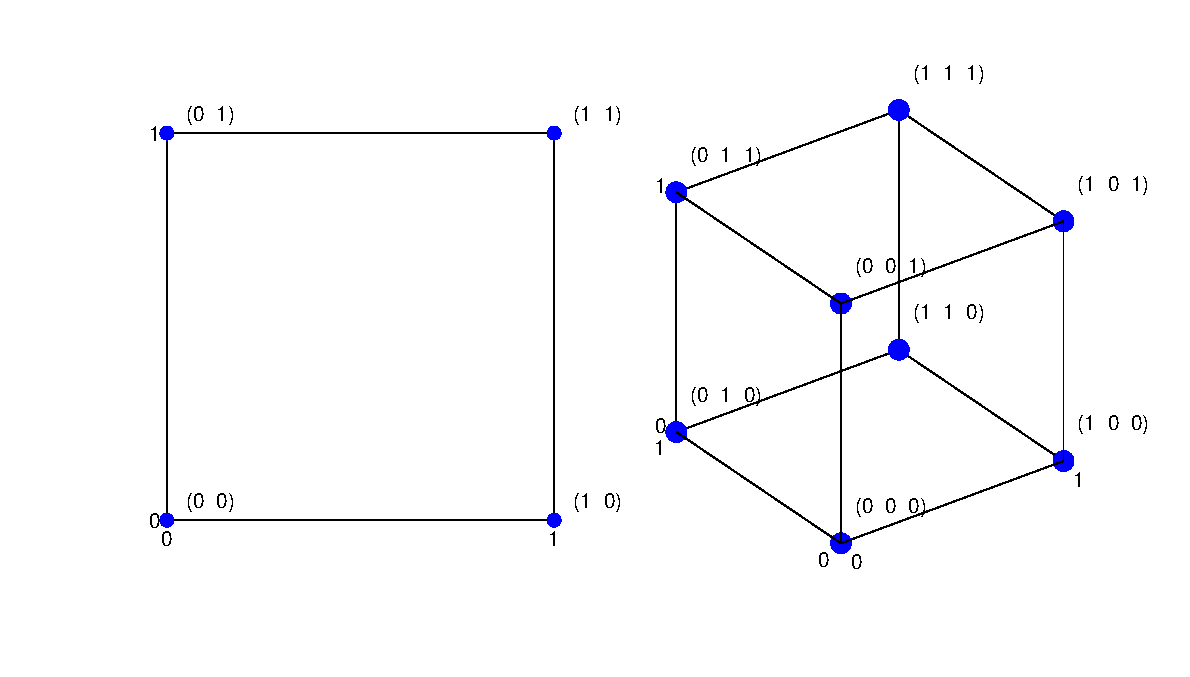
\includegraphics[width=4.5in]{figures/BernoulliDataSpace2and3}}
\end{figure}

\begin{definition}[Statistic]\label{D:Statistic}
A {\bf statistic} $T$ is any
%(measurable)
function of the data:
\[
T(x) : \Xz \to \Tz \ .
\]
Thus, a statistic $T$ is also an RV that takes values in the space $\Tz$.  When $x \in \Xz$ is the realisation of an experiment, we let $T(x)=t$ denote the corresponding realisation of the statistic $T$. Sometimes we use $T_n(X)$ and $\Tz_n$ to emphasise that $X$ is an $n$-dimensional random vector, i.e.~$\Xz \subset \Rz^n$
\end{definition}

\begin{classwork}[Is data a statistic?]
Is the RV $X$, for which the realisation is the observed data $X(\omega)=x$, a statistic?  In other words, is the data a statistic? [Hint: consider the identity map $T(x)=x: \Xz \to \Tz=\Xz$.]
\end{classwork}

Next, we define two important statistics called the {\bf sample mean} and {\bf sample variance}.  Since they are obtained from the sample data, they are called {\bf sample moments}, as opposed to the {\bf population moments}.  The corresponding population moments are $\E(X_1)$ and $\V(X_1)$, respectively.
\begin{definition}[Sample Mean]\label{D:SampleMean}
From a given a sequence of RVs $X_1,X_2,\ldots,X_n$, we may obtain another RV called the $n$-samples mean or simply the sample mean:
\begin{equation}\label{E:SampleMeanRV}
T_n( \ (X_1,X_2,\ldots,X_n) \ ) = \overline{X}_n( \ (X_1,X_2,\ldots,X_n) \ ) := \frac{1}{n} \sum_{i=1}^n X_i  \ .
\end{equation}
For brevity, we write $$\overline{X}_n( \ (X_1,X_2,\ldots,X_n) \ ) \quad \text{as} \quad \overline{X}_n \ ,$$ and its realisation $$\overline{X}_n( \ (x_1,x_2,\ldots,x_n) \ ) \quad \text{as} \quad \overline{x}_n \ .$$
\end{definition}
Note that the expectation and variance of $\overline{X}_n$ are:
\begin{eqnarray}
\E(\overline{X}_n) &=& \E \left(  \frac{1}{n} \sum_{i=1}^n X_i \right) \qquad \text{{\scriptsize[by \hyperref[E:SampleMeanRV]{definition \eqref{E:SampleMeanRV}}]}} \notag \\
&=&  \frac{1}{n} \sum_{i=1}^n \E \left( X_i \right) \qquad \text{{\scriptsize [by \hyperref[E:EofLinCombofRVs]{property \eqref{E:EofLinCombofRVs}}]}} \notag
\end{eqnarray}
Furthermore, if every $X_i$ in the original sequence of RVs $X_1,X_2,\ldots$ is {\bf identically} distributed with the same expectation, by convention $\E(X_1)$, then:
\begin{equation}\label{E:ExpOfSampleMeanOfIDSeq}
\E(\overline{X}_n)
= \frac{1}{n} \sum_{i=1}^n \E \left( X_i \right)
=  \frac{1}{n} \sum_{i=1}^n \E \left( X_1 \right)
=  \frac{1}{n} \ n \ \E \left( X_1 \right)  = \E \left( X_1 \right) \ .
\end{equation}
Similarly, we can show that:
\begin{eqnarray}
\V(\overline{X}_n) &=& \V \left(  \frac{1}{n} \sum_{i=1}^n X_i \right) \qquad \text{{\scriptsize[by \hyperref[E:SampleMeanRV]{definition \eqref{E:SampleMeanRV}}]}} \notag \\
&=& \left( \frac{1}{n} \right)^2  \V \left( \sum_{i=1}^n X_i \right) \qquad \text{{\scriptsize [by \hyperref[E:VofAffineofRVs]{property \eqref{E:VofAffineofRVs}}]}} \notag
\end{eqnarray}
Furthermore, if the original sequence of RVs $X_1,X_2,\ldots$ is {\bf independently} distributed then:
\begin{eqnarray}
\V(\overline{X}_n)
= \left( \frac{1}{n} \right)^2 \V \left(  \sum_{i=1}^n X_i \right)
=  \frac{1}{n^2} \ \sum_{i=1}^n \V \left( X_i \right) \qquad \text{{\scriptsize [by \hyperref[E:VofLinCombofRVs]{property \eqref{E:VofLinCombofRVs}}]}} \notag
\end{eqnarray}
Finally, if the original sequence of RVs $X_1,X_2,\ldots$ is {\bf independently and identically} distributed with the same variance ($\V(X_1)$ by convention) then:
\begin{equation}\label{E:VarOfSampleMeanOfIIDSeq}
\V(\overline{X}_n)
=  \frac{1}{n^2} \ \sum_{i=1}^n \V \left( X_i \right)
= \frac{1}{n^2} \ \sum_{i=1}^n \V \left( X_1 \right)
=  \frac{1}{n^2} \ n \ \V \left( X_1 \right)
=  \frac{1}{n} \ \V \left( X_1 \right) \ .
\end{equation}

\begin{labwork}[Sample mean]\label{LW:XsFromUni01Twstr101mean}
After initializing the fundamental sampler, we draw five samples and then obtain the sample mean using the {\sc Matlab} function {\tt mean}.  In the following, we will reuse the samples stored in the array {\tt XsFromUni01Twstr101}.
\begin{VrbM}
>> rand('twister',101); % initialise the fundamental Uniform(0,1) sampler
>> XsFromUni01Twstr101=rand(1,5); % simulate n=5 IID samples from Uniform(0,1) RV
>> SampleMean=mean(XsFromUni01Twstr101);% find sample mean
>> disp(XsFromUni01Twstr101); % The data-points x_1,x_2,x_3,x_4,x_5 are:
    0.5164    0.5707    0.0285    0.1715    0.6853
>> disp(SampleMean); % The Sample mean is :
    0.3945
\end{VrbM}
We can thus use {\tt mean} to obtain the sample mean $\overline{x}_n$ of $n$ sample points $x_1,x_2,\ldots,x_n$.

We may also obtain the sample mean using the {\tt sum} function and a division by sample size:
\begin{VrbM}
>> sum(XsFromUni01Twstr101) % take the sum of the elements of the XsFromUni01Twstr101 array
ans =    1.9723
>> sum(XsFromUni01Twstr101) / 5 % divide the sum by the sample size 5
ans =    0.3945
\end{VrbM}

We can also obtain the sample mean via matrix product or multiplication as follows:
\begin{VrbM}
>> size(XsFromUni01Twstr101) % size(SomeArray) gives the size or dimensions of the arrar SomeArray
ans =     1     5
>> ones(5,1) % here ones(5,1) is an array of 1's with size or dimension 5 X 1
ans =
     1
     1
     1
     1
     1
>> XsFromUni01Twstr101 * ones(5,1) % multiplying an 1 X 5 matrix with a 5 X 1 matrix of Ones
ans =    1.9723
>> XsFromUni01Twstr101 * ( ones(5,1) * 1/5) % multiplying an 1 X 5 matrix with a 5 X 1 matrix of 1/5 's
ans =    0.3945
\end{VrbM}
\end{labwork}

\begin{definition}[Sample Variance \& Standard Deviation]
From a given a sequence of random variables $X_1,X_2,\ldots,X_n$, we may obtain another statistic called the $n$-samples variance or simply the sample variance :
\begin{equation}\label{E:SampleVarianceRV}
T_n( \ (X_1,X_2,\ldots,X_n) \ ) = S^2_n( \ (X_1,X_2,\ldots,X_n) \ )  := \frac{1}{n-1} \sum_{i=1}^n {(X_i - \overline{X}_n)^2}  \ .
\end{equation}
For brevity, we write $S^2_n( \ (X_1,X_2,\ldots,X_n) \ )$ as $S^2_n$ and its  realisation $S^2_n( \ (x_1,x_2,\ldots,x_n) \ )$ as $s^2_n$.

Sample standard deviation is simply the square root of sample variance:
\begin{equation}\label{E:SampleStdDevRV}
S_n( \ (X_1,X_2,\ldots,X_n) \ ) = \sqrt{S^2_n( \ (X_1,X_2,\ldots,X_n) \ )}
\end{equation}
For brevity, we write $S_n( \ (X_1,X_2,\ldots,X_n) \ )$ as $S_n$ and its  realisation $S_n( \ (x_1,x_2,\ldots,x_n) \ )$ as $s_n$.
\end{definition}
Once again, if $X_1,X_2,\ldots,X_n \overset{\IID}{\sim} X_1$, the expectation of the sample variance is:
\[
\E(S^2_n) = \V(X_1) \ .
\]
\begin{labwork}[Sample variance and sample standard deviation]\label{LW:XsFromUni01Twstr101varstd}
We can compute the sample variance and sample standard deviation for the five samples stored in the array {\tt XsFromUni01Twstr101} from \hyperref[LW:XsFromUni01Twstr101mean]{Labwork \ref*{LW:XsFromUni01Twstr101mean}} using {\sc Matlab}'s functions {\tt var} and {\tt std}, respectively.
\begin{VrbM}
>> disp(XsFromUni01Twstr101); % The data-points x_1,x_2,x_3,x_4,x_5 are :
    0.5164    0.5707    0.0285    0.1715    0.6853
>> SampleVar=var(XsFromUni01Twstr101);% find sample variance
>> SampleStd=std(XsFromUni01Twstr101);% find sample standard deviation
>> disp(SampleVar) % The sample variance is:
    0.0785
>> disp(SampleStd) % The sample standard deviation is:
    0.2802
\end{VrbM}
\end{labwork}
It is important to bear in mind that the statistics such as sample mean and sample variance are random variables and have an underlying distribution.

\begin{definition}[Order Statistics]
Suppose $X_1,X_2,\ldots,X_n \overset{\IID}{\sim} F$, where $F$ is the DF from the set of all DFs over the real line.  Then, the $n$-sample {\bf order statistics} $X_{([n])}$ is:
\begin{equation}\label{E:OrderStatistics}
X_{([n])}( \ (X_1,X_2,\ldots,X_n) \ ) := \left(  X_{(1)},X_{(2)}, \ldots X_{(n)} \right), \text{ such that, }
 X_{(1)} \leq X_{(2)} \leq \ldots \leq X_{(n)}  \ .
\end{equation}
For brevity, we write $X_{([n])}( \ (X_1,X_2,\ldots,X_n) \ )$ as $X_{([n])}$ and its realisation $X_{([n])}( \ (x_1,x_2,\ldots,x_n) \ )$ as $x_{([n])} = (  x_{(1)},x_{(2)}, \ldots x_{(n)} )$.
\end{definition}
Without going into the details of how to sort the data in ascending order to obtain the order statistics (an elementary topic of an Introductory Computer Science course), we simply use {\sc Matlab}'s function {\tt sort} to obtain the order statistics, as illustrated in the following example.
\begin{labwork}[Order statistics and sorting]\label{LW:SortedXsFromUni01Twstr101}
The order statistics for the five samples stored in {\tt XsFromUni01Twstr101} from \hyperref[LW:XsFromUni01Twstr101mean]{Labwork \ref*{LW:XsFromUni01Twstr101mean}} can be computed using {\tt sort} as follows:
\begin{VrbM}
>> disp(XsFromUni01Twstr101); % display the sample points
    0.5164    0.5707    0.0285    0.1715    0.6853
>> SortedXsFromUni01Twstr101=sort(XsFromUni01Twstr101); % sort data
>> disp(SortedXsFromUni01Twstr101); % display the order statistics
    0.0285    0.1715    0.5164    0.5707    0.6853
\end{VrbM}
Therefore, we can use {\tt sort} to obtain our order statistics $x_{(1)},x_{(2)},\ldots,x_{(n)}$ from $n$ sample points $x_1,x_2,\ldots,x_n$.
\end{labwork}

Next, we will introduce a family of common statistics, called the $q^{\text{th}}$ quantile, by first defining the function:
\begin{definition}[Inverse DF or Inverse CDF or Quantile Function]
Let $X$ be an RV with DF $F$.  The {\bf inverse DF} or {\bf inverse CDF} or {\bf quantile function} is:
\begin{equation}\label{E:InverseCDF}
F^{[-1]}(q) := \inf { \{ x: F(x) > q \}}, \quad \text{ for some $q \in [0,1]$} \ .
\end{equation}
If $F$ is strictly increasing and continuous then $F^{[-1]}(q)$ is the unique $x \in \Rz$ such that $F(x)=q$.
\end{definition}
A {\bf functional} is merely a function of another function.  Thus, $T(F): \{ \text{All DFs }\} \to \Tz$, being a map or function from the space of DFs to its range $\Tz$, is a functional.  Some specific examples of functionals we have already seen include:
\begin{enumerate}
\item The {\bf mean} of RV $X \sim F$ is a function of the DF $F$:
\[
T(F) = \E(X) = \int x\,dF(x) \ .
\]
\item The {\bf variance} of RV $X \sim F$ is a function of the DF $F$:
\[
T(F) = \E(X-\E(X))^2 = \int (x-\E(X))^2\,dF(x) \ .
\]
\item The {\bf value of DF at a given $x \in \Rz$} of RV $X \sim F$ is also a function of DF $F$:
\[
T(F) = F(x) \  .
\]
\end{enumerate}
Other functionals of $F$ that depend on the quantile function $F^{[-1]}$ are:
\begin{enumerate}
\item The {\bf $q^{\text{th}}$ quantile} of RV $X \sim F$:
\[
T(F) = F^{[-1]}(q) \ \text{ where } q \in [0,1] \ .
\]
\item The {\bf first quartile} or the {\bf $0.25^{\text{th}}$ quantile} of the RV $X \sim F$:
\[
T(F) = F^{[-1]}(0.25) \ .
\]
\item The {\bf median} or the {\bf second quartile} or the {\bf $0.50^{\text{th}}$ quantile} of the RV $X \sim F$:
\[
T(F) = F^{[-1]}(0.50) \  .
\]
\item The {\bf third quartile} or the {\bf $0.75^{\text{th}}$ quantile} of the RV $X \sim F$:
\[
T(F) = F^{[-1]}(0.75) \ .
\]
\end{enumerate}

\begin{definition}[Empirical Distribution Function (EDF or ECDF)]\label{D:ECDF}
Suppose we have $n$ IID RVs, $X_1,X_2,\ldots,X_n \overset{\IID}{\sim} F$, where $F$ is a DF from the set of all DFs over the real line.  Then, the $n$-sample empirical distribution function (EDF or ECDF) is the discrete  distribution function $\widehat{F}_n$ that puts a probability mass of $1/n$ at each sample or data point $x_i$:
\begin{eqnarray} \label{E:ECDF}
\widehat{F}_n(x) = \frac{ \sum_{i=1}^n \BB{1}(X_i \leq x) }{n} \ ,  & \quad where \qquad
\BB{1}(X_i \leq x) :=
\begin{cases}
& 1  \quad \text{if $x_i \leq x$} \\
& 0  \quad \text{if $x_i > x$}
\end{cases}
\end{eqnarray}
\end{definition}

\begin{labwork}[Plot of empirical CDF]\label{LW:ECDF}
Let us plot the ECDF for the five samples drawn from the $Uniform(0,1)$ RV in \hyperref[LW:XsFromUni01Twstr101mean]{Labwork \ref*{LW:XsFromUni01Twstr101mean}} using the {\sc Matlab} function {\tt ECDF}. %(given in \hyperref[Mf:ECDF]{Labwork \ref*{Mf:ECDF}}).
Let us super-impose the samples and the true DF as depicted in \hyperref[F:plotUniform01ECDF5]{Figure \ref*{F:plotUniform01ECDF5}} with the following script:
{\VrbMf[label=plotunifecdf.m]{scripts/plotunifecdf.m}}

\begin{figure}[htpb]
\caption{Plot of the DF of $\uniform(0,1)$, five IID samples from it, and the ECDF $\widehat{F}_5$ for these five data points $x=(x_1,x_2,x_3,x_4,x_5)=(0.5164,    0.5707,    0.0285,    0.1715,    0.6853)$ that jumps by $1/5=0.20$ at each of the five samples.\label{F:plotUniform01ECDF5}}
\centering   \makebox{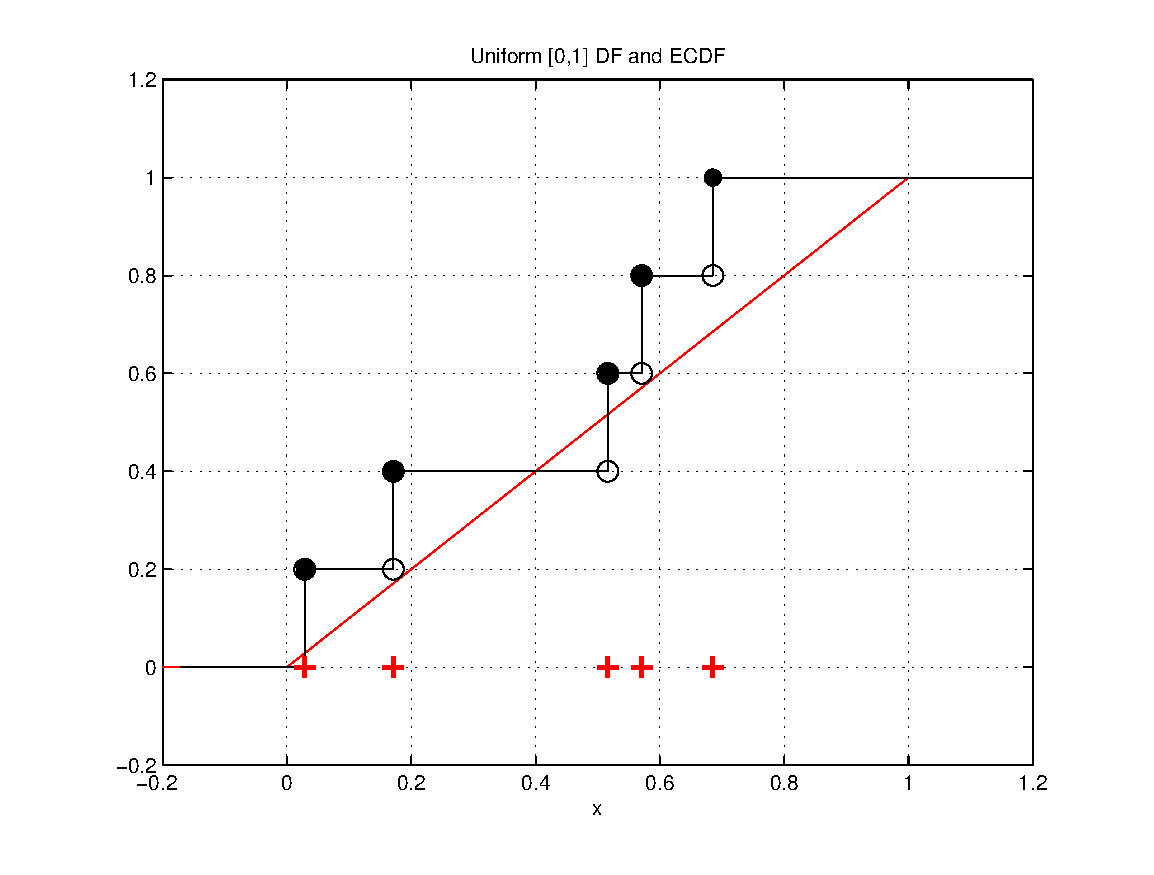
\includegraphics[width=4.5in]{figures/plotUniform01ECDF5}}
\end{figure}
\end{labwork}

\begin{definition}[$q^{\text{th}}$ Sample Quantile]
For some $q \in [0,1]$ and $n$ IID RVs $X_1,X_2,\ldots,X_n \overset{\IID}{\sim} F$, we can obtain the ECDF $\widehat{F}_n$ using \eqref{E:ECDF}.  The {\bf $q^{\text{th}}$ sample quantile} is defined as the statistic (statistical functional):
\begin{equation}\label{E:qthSampleQuantile}
T(\widehat{F}_n) = \widehat{F}_n^{[-1]}(q) := \inf{ \{ x:  \widehat{F}_n^{[-1]}(x) \geq q \} } \ .
\end{equation}
By replacing $q$ in this definition of the $q^{\text{th}}$ sample quantile by $0.25$, $0.5$ or $0.75$, we obtain the first, second ({\bf sample median}) or third {\bf sample quartile}, respectively.
\end{definition}

The following algorithm can be used to obtain the $q^{\text{th}}$ sample quantile of $n$ IID samples $(x_1,x_2,\ldots,x_n)$ on the basis of their order statistics $(x_{(1)},x_{(2)},\ldots,x_{(n)})$.
\begin{algorithm}
\caption{$q^{\text{th}}$ Sample Quantile of Order Statistics}
\label{A:qthSampleQuantile}
\begin{algorithmic}[1]
\STATE {
{\it input:}
\begin{enumerate}
\item $q$ in the $q^{\text{th}}$ sample quantile, i.e.~the argument $q$ of $ \widehat{F}_n^{[-1]}(q)$,
\item order statistic $(x_{(1)},x_{(2)},\ldots,x_{(n)})$, i.e.~the sorted $(x_1,x_2,\ldots,x_n)$, where $n>0$.
\end{enumerate}
}
\STATE {\it output:} $ \widehat{F}_n^{[-1]}(q)$, the $q^{\text{th}}$ sample quantile
\STATE $i \gets \lfloor (n-1) q \rfloor$
\STATE $\delta \gets (n-1) q - i$
\IF {$i = n-1$}
\STATE {$ \widehat{F}_n^{[-1]}(q) \gets x_{(i+1)}$}
\ELSE
\STATE $ \widehat{F}_n^{[-1]}(q) \gets (1 - \delta) x_{(i+1)} + \delta x_{(i+2)}$
\ENDIF
\STATE {{\it return:} $ \widehat{F}_n^{[-1]}(q)$}
\end{algorithmic}
\end{algorithm}

The $q^{\text{th}}$ sample quantile, $ \widehat{F}_n^{[-1]}(q)$, is found by interpolation from the order statistics $(x_{(1)},x_{(2)},\ldots,x_{(n)})$ of the $n$ data points $(x_1,x_2,\ldots,x_n)$, using the formula:
\[
 \widehat{F}_n^{[-1]}(q) = (1 - \delta) x_{(i+1)} + \delta x_{(i+2)}, \quad \text{where, }
\quad i = \lfloor (n-1) q \rfloor  \quad \text{ and }
\quad \delta = (n-1) q -  \lfloor (n-1) q \rfloor \ .
\]
Thus, the {\bf sample minimum} of the data points $(x_1,x_2,\ldots,x_n)$ is given by $ \widehat{F}_n^{[-1]}(0)$, the {\bf sample maximum} is given by $ \widehat{F}_n^{[-1]}(1)$ and the {\bf sample median} is given by $ \widehat{F}_n^{[-1]}(0.5)$, etc.
\begin{labwork}[The $q^{\text{th}}$ sample quantile]\label{LW:qthSampleQuantile}
Use the implementation of \hyperref[A:qthSampleQuantile]{Algorithm \ref*{A:qthSampleQuantile}} %in \hyperref[Mf:qthSampleQuantile]{Labwork \ref*{Mf:qthSampleQuantile}}
as the {\sc Matlab} function {\tt qthSampleQuantile} to find the $q^{\text{th}}$ sample quantile of two simulated data arrays:
\begin{enumerate}
\item {\tt SortedXsFromUni01Twstr101}, the order statistics that was constructed in \hyperref[LW:SortedXsFromUni01Twstr101]{Labwork \ref*{LW:SortedXsFromUni01Twstr101}} and
\item Another sorted array of $7$ samples called {\tt SortedXs}
\end{enumerate}
\begin{VrbM}
>> disp(SortedXsFromUni01Twstr101)
    0.0285    0.1715    0.5164    0.5707    0.6853
>> rand('twister',420);
>> SortedXs=sort(rand(1,7));
>> disp(SortedXs)
    0.1089    0.2670    0.3156    0.3525    0.4530    0.6297    0.8682
>> for q=[0, 0.25, 0.5, 0.75, 1.0]
       disp([q, qthSampleQuantile(q,SortedXsFromUni01Twstr101) ...
                qthSampleQuantile(q,SortedXs)])
   end
         0    0.0285    0.1089
    0.2500    0.1715    0.2913
    0.5000    0.5164    0.3525
    0.7500    0.5707    0.5414
    1.0000    0.6853    0.8682
\end{VrbM}
\end{labwork}

%\subsection{Exploring Data and Statistics}\label{S:ExploringData}

\subsection{Univariate Data}
A {\bf histogram} is a graphical representation of the frequency with which elements of a data array:
$$x = (x_1,x_2,\ldots,x_n) \ ,$$
of real numbers fall within each of the $m$ intervals or {\bf bins} of some {\bf interval partition}:
$$b := ( b_1, b_2, \ldots, b_m ) := ( [\underline{b}_1,\overline{b}_1], [\underline{b}_2,\overline{b}_2], \ldots, [\underline{b}_m,\overline{b}_m] )$$
of the {\bf data range} of $x$ given by the closed interval:
$$\C{R}(x) := [\min \{x_1,x_2,\ldots,x_n \}, \max \{x_1,x_2,\ldots,x_n \}] \ .$$
Elements of this partition $b$ are called bins, their mid-points are called {\bf bin centres}:
$$c := ( c_1, c_2, \ldots, c_m ) := ( (\underline{b}_1+\overline{b}_1)/2, (\underline{b}_2 + \overline{b}_2)/2, \ldots, (\underline{b}_m + \overline{b}_m)/2 )$$
and their overlapping boundaries, i.e.~$\overline{b}_i=\underline{b}_{i+1}$ for $1 \leq i < m$, are called {\bf bin edges}:
$$d := (d_1,d_2,\ldots,d_{m+1}) := (\underline{b}_1, \underline{b}_2, \ldots, \underline{b}_{m-1}, \underline{b}_m, \overline{b}_m) \ .$$
For a given partition of the data range $\C{R}(x)$ or some superset of $\C{R}(x)$, three types of histograms are possible: frequency histogram, relative frequency histogram and density histogram.  Typically, the partition $b$ is assumed to be composed of $m$ overlapping intervals of the same width $w=\overline{b}_i - \underline{b}_i$ for all $i=1,2,\ldots,m$.  Thus, a histogram can be obtained by a set of bins along with their corresponding {\bf heights}:
$$h = (h_1,h_2,\ldots,h_m) \ , \text{ where } h_k := g(\# \{x_i : x_i \in b_k\} )$$
Thus, $h_k$, the height of the $k$-th bin, is some function $g$ of the number of data points that fall in the bin $b_k$ Formally, a histogram is a sequence of ordered pairs:
$$\left(  (b_1,h_1), (b_2,h_2), \ldots, (b_m,h_m) \right) \ .$$

Given a partition $b$, a {\bf frequency histogram} is the histogram:
$$\left(  (b_1,h_1), (b_2,h_2), \ldots, (b_m,h_m) \right) \ , \text{ where } h_k := \# \{x_i : x_i \in b_k\} \ ,$$
a {\bf relative frequency histogram} is the histogram:
$$\left(  (b_1,h_1), (b_2,h_2), \ldots, (b_m,h_m) \right) \ , \text{ where } h_k := n^{-1} \# \{x_i : x_i \in b_k\} \ ,$$
and a {\bf density histogram} is the histogram:
$$\left(  (b_1,h_1), (b_2,h_2), \ldots, (b_m,h_m) \right) \ , \text{ where } h_k := (w_k n)^{-1} \# \{x_i : x_i \in b_k\} \ , w_k := \overline{b}_k - \underline{b}_k \ .$$

\begin{figure}[htpb]
\caption{Frequency, Relative Frequency and Density Histograms\label{F:FreqRelFreqDensityHistograms100Unif01MT5489}}
\centering   \makebox{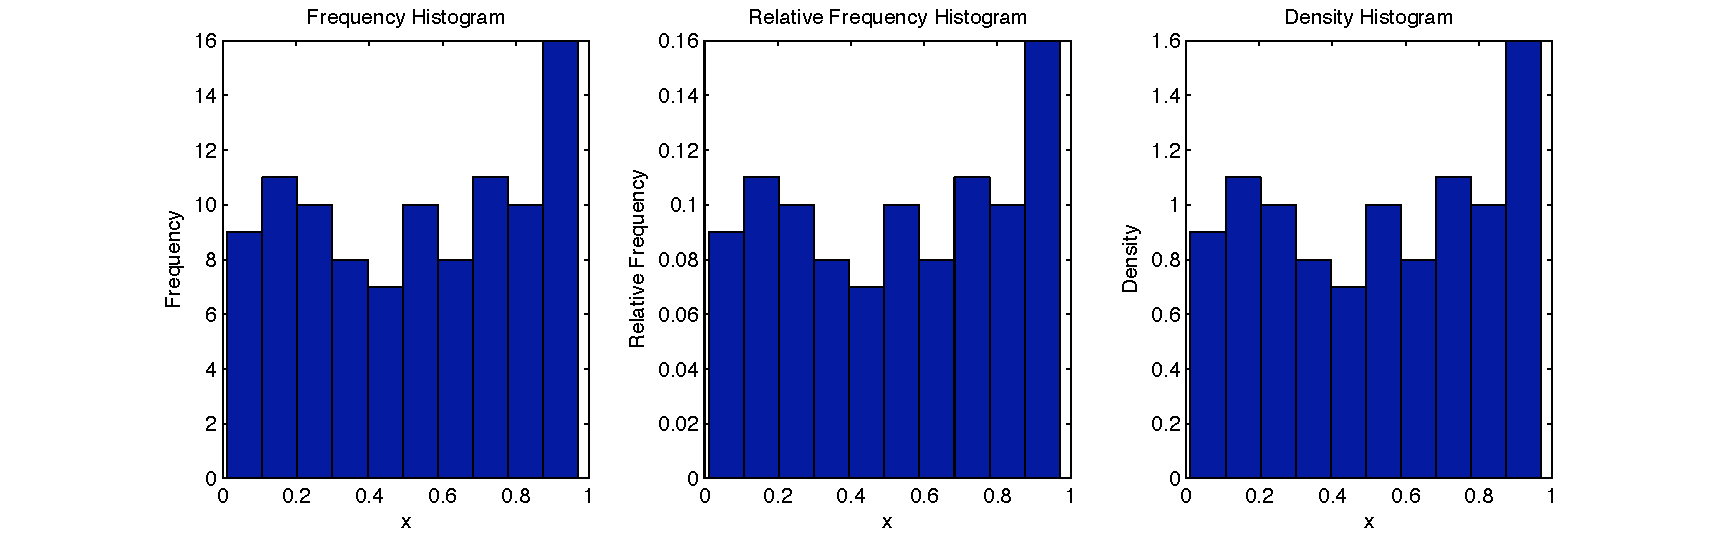
\includegraphics[width=6.5in]{figures/FreqRelFreqDensityHistograms100Unif01MT5489}}
\end{figure}

\begin{labwork}[Histograms with specified number of bins for univariate data]\label{LW:hist}
Let us use samples from the {\tt rand('twister',5489)} as our data set $x$ and plot various histograms.  Let us use {\tt hist} function (read {\tt help hist}) to make a default histogram with ten bins.  Then we can make three types of histogarms as shown in \hyperref[F:FreqRelFreqDensityHistograms100Unif01MT5489]{Figure~\ref*{F:FreqRelFreqDensityHistograms100Unif01MT5489}}  as follows:
\begin{VrbM}
>> rand('twister',5489);
>> x=rand(1,100); % generate 100 PRNs
>> hist(x) % see what default hist does in Figure Window
>> % Now let us look deeper into the last hist call
>> [Fs, Cs] = hist(x) % Cs is the bin centers and Fs is the frequencies of data set x
Fs =
     9    11    10     8     7    10     8    11    10    16
Cs =
    0.0598    0.1557    0.2516    0.3474    0.4433    0.5392    0.6351    0.7309    0.8268    0.9227
>> % produce a histogram plot the last argument 1 is the width value for immediately adjacent bars -- help bar
>> bar(Cs,Fs,1) % create a frequency histogram
>> bar(Cs,Fs/100,1) % create a relative frequency histogram
>> bar(Cs,Fs/(0.1*100),1) % create a density histogram (area of bars sum to 1)
>> sum(Fs/(0.1*100) .* ones(1,10)*0.1) % checking if area does sum to 1
>> ans = 1
\end{VrbM}
Try making a density histogram with 1000 samples from {\tt rand} with 15 bins.  You can specify the number of bins by adding an extra argument to {\tt hist}, for e.g. {\tt [Fs, Cs] = hist(x,15)} will produce 15 bins of equal width over the data range $\C{R}(x)$.
\end{labwork}

\begin{labwork}[Stem plots and ECDF plots for univariate data]\label{LW:StemEcdf}
We can also visualise the 100 data points in the array {\tt x} using stem plot and ECDF plot as shown in \hyperref[F:StemECDF100Unif01MT5489]{Figure~\ref*{F:StemECDF100Unif01MT5489}} as follows:
\begin{VrbM}
>> rand('twister',5489);
>> x=rand(1,100); % produce 100 samples with rand
>> stem(x,'.') % make a stem plot of the 100 data points in x (the option '.' gives solid circles for x)
>>% ECDF (type help ECDF) plot is extended to left and right by .2 and .6, respectively
>>% (second parameter 6 makes the dots in the plot smaller).
>> ECDF(x,6,.2,.6);
\end{VrbM}
\end{labwork}

\begin{figure}[htpb]
\caption{Frequency, Relative Frequency and Density Histograms\label{F:StemECDF100Unif01MT5489}}
\centering   \makebox{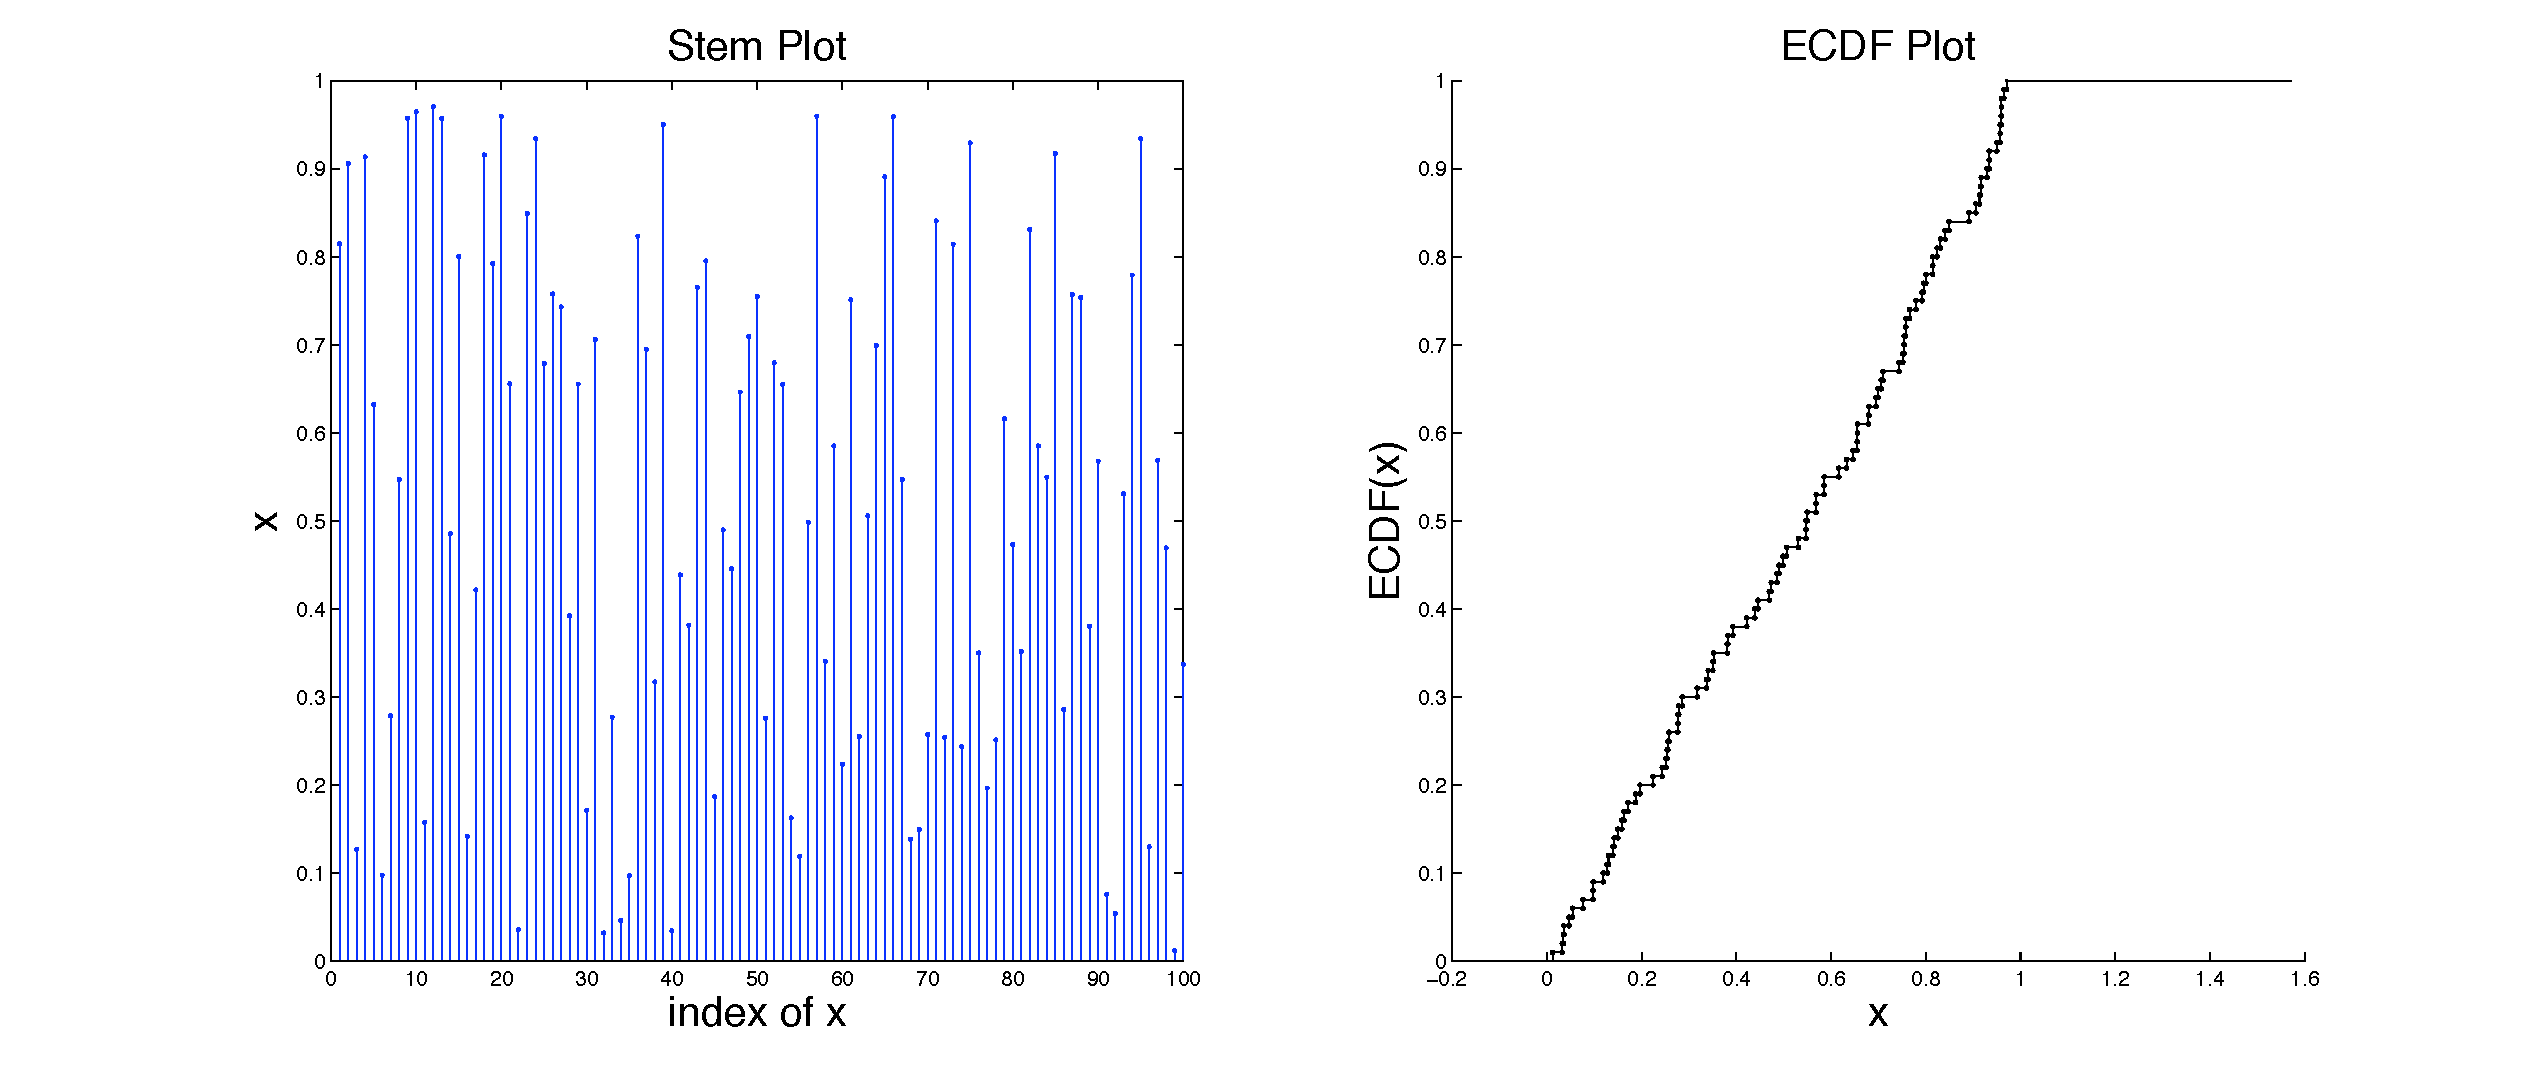
\includegraphics[width=6.5in]{figures/StemECDF100Unif01MT5489}}
\end{figure}

We can also visually summarise univariate data using the {\bf box plot} or {\bf box-whisker plot} available in the Stats Toolbox of {\sc Matlab}.  These family of plots display a set of sample quantiles, typically they are include, the median, the first and third quartiles and the minimum and maximum values of our data array $x$.

\subsection{Bivariate Data}
By bivariate data array $x$ we mean a $2 \times n$ matrix of real numbers or equivalently $n$ ordered pairs of points $(x_{1,i},x_{2,i})$ as $i=1,2,\ldots,n$.  The most elementary visualisation of these $n$ ordered pairs is in orthogonal Cartesian co-ordinates.  Such plots are termed 2D {\bf scatter plots} in statistics.
\begin{labwork}[Visualising bivariate data]\label{LW:2DScatter}
Let us generate a $2 \times 5$ array representing samples of $5$ ordered pairs sampled uniformly at random over the unit square $[0,1] \times [0,1]$.  We can make 2D scatter plot as shown in \hyperref[F:Twister5489X2x5Scatter2D]{Figure~\ref*{F:Twister5489X2x5Scatter2D}}  as follows:
\begin{VrbM}
>> rand('twister',5489);
>> x=rand(2,5)% create a sequence of 5 ordered pairs uniformly from unit square [0,1]X[0,1]
x =
    0.8147    0.1270    0.6324    0.2785    0.9575
    0.9058    0.9134    0.0975    0.5469    0.9649
>> plot(x(1,:),x(2,:),'x') % a 2D scatter plot with marker cross or 'x'
>> plot(x(1,:),x(2,:),'x', 'MarkerSize',15) % a 2D scatter plot with marker cross or 'x' and larger Marker size
>> xlabel('x_1'); ylabel('x_2'); % label the axes
\end{VrbM}
\end{labwork}

\begin{figure}[htpb]
\caption{2D Scatter Plot\label{F:Twister5489X2x5Scatter2D}}
\centering   \makebox{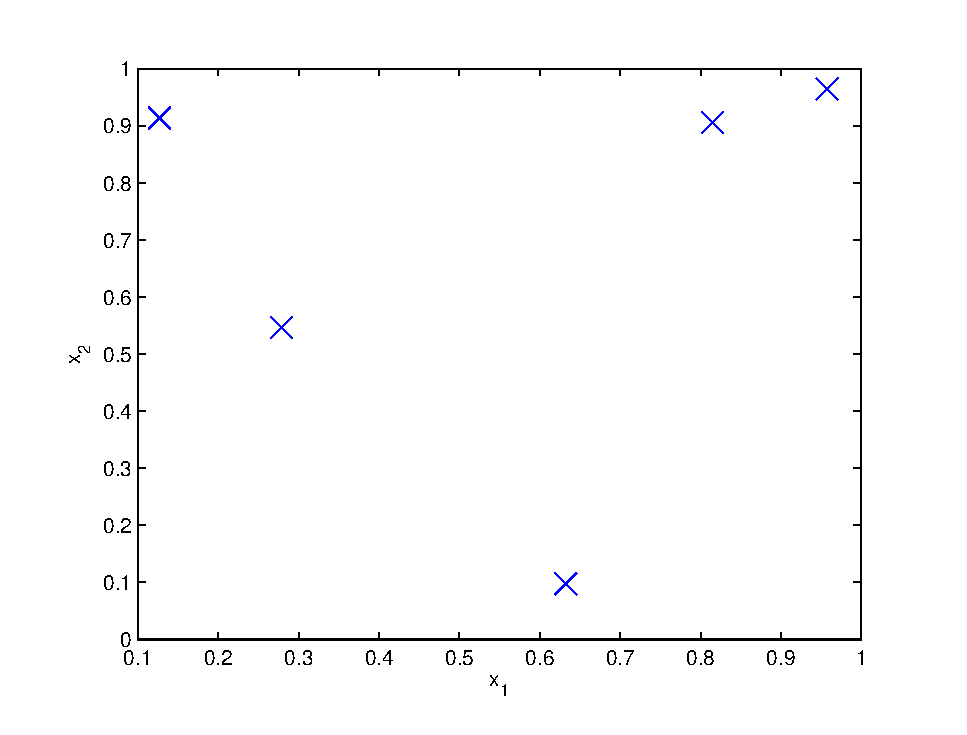
\includegraphics[width=4.5in]{figures/Twister5489X2x5Scatter2D}}
\end{figure}

There are several other techniques for visualising bivariate data, including,
2D histograms, surface plots, heat plots, and we will encounter some of them in the sequel.

\subsection{Trivariate Data}
Trivariate data is more difficult to visualise on paper but playing around with the rotate 3D feature in \Matlab's Figure window can help bring a lot more perspective.

\begin{labwork}[Visualising trivariate data]\label{LW:3DScatter}
We can make {\bf 3D scatter plots} as shown in \hyperref[F:Twister5489X3x5Scatter3D]{Figure~\ref*{F:Twister5489X3x5Scatter3D}}  as follows:
\begin{VrbM}
>> rand('twister',5489);
>> x=rand(3,5)% create a sequence of 5 ordered triples uniformly from unit cube [0,1]X[0,1]X[0,1]
x =
    0.8147    0.9134    0.2785    0.9649    0.9572
    0.9058    0.6324    0.5469    0.1576    0.4854
    0.1270    0.0975    0.9575    0.9706    0.8003
>> plot3(x(1,:),x(2,:),x(3,:),'x') % a simple 3D scatter plot with marker 'x'
>>% a more interesting one with options that control marker type, line-style,
>>% colour in [Red Green Blue] values and marker size - read help plot3 for more options
>> plot3(x(1,:),x(2,:),x(3,:),'Marker','*','LineStyle','none','Color',[1 0 1],'MarkerSize',15)
>> plot3(x(1,:),x(2,:),x(3,:),'m*','MarkerSize',15) % makes same  figure as before but shorter to write
>> box on % turn on the box and see the effect on the Figure
>> grid on % turn on the grid and see the effect on the Figure
>> xlabel('x_1'); ylabel('x_2'); zlabel('x_3'); % assign labels to x,y and z axes
\end{VrbM}
Repeat the visualisation below with a larger array, say {\tt x=rand(3,1000)}, and use the rotate 3D feature in the Figure window to visually explore the samples in the unit cube.  Do they seem to be uniformly distributed inside the unit cube?
\end{labwork}

\begin{figure}[htpb]
\caption{3D Scatter Plot\label{F:Twister5489X3x5Scatter3D}}
\centering   \makebox{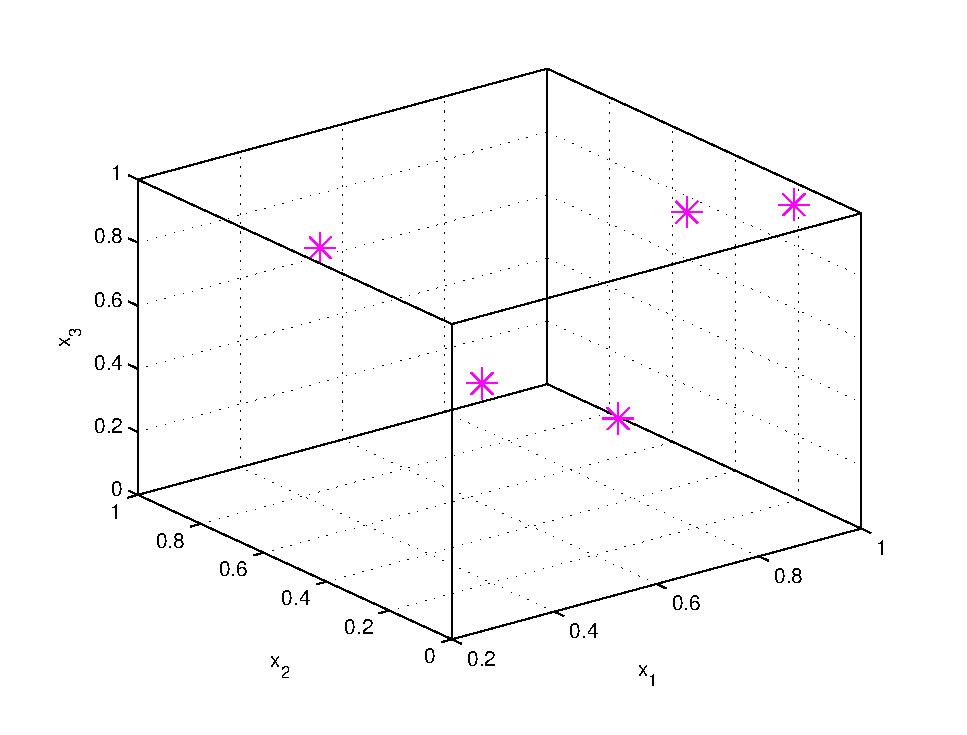
\includegraphics[width=4.5in]{figures/Twister5489X3x5Scatter3D}}
\end{figure}


There are several other techniques for visualising trivariate data, including,
iso-surface plots, moving surface or heat plots, and you will encounter some of them in the future.

\subsection{Multivariate Data}
For high-dimensional data in $d$-dimensional space $\Rz^d$ with $d \geq 3$ you have to look at several lower dimensional projections of the data.  We can simultaneously look at 2D scatter plots for every pair of co-ordinates $\{(i,j) \in \{1,2,\ldots,d\}^2 : i \neq j \}$ and at histograms for every co-ordinate $i \in \{1,2,\ldots,d\}$ of the $n$ data points in $\Rz^d$.  Such a set of low-dimensional projections can be conveniently represented in a $d \times d$ matrix of plots called a {\bf matrix plot}.

\begin{figure}[htpb]
\caption{Plot Matrix of uniformly generated data in $[0,1]^5$\label{F:Twister5489X100x5PlotMatrixFirst6andAll100}}
\centering
\mbox{\subfigure[First six samples]{\hspace{-1.cm} 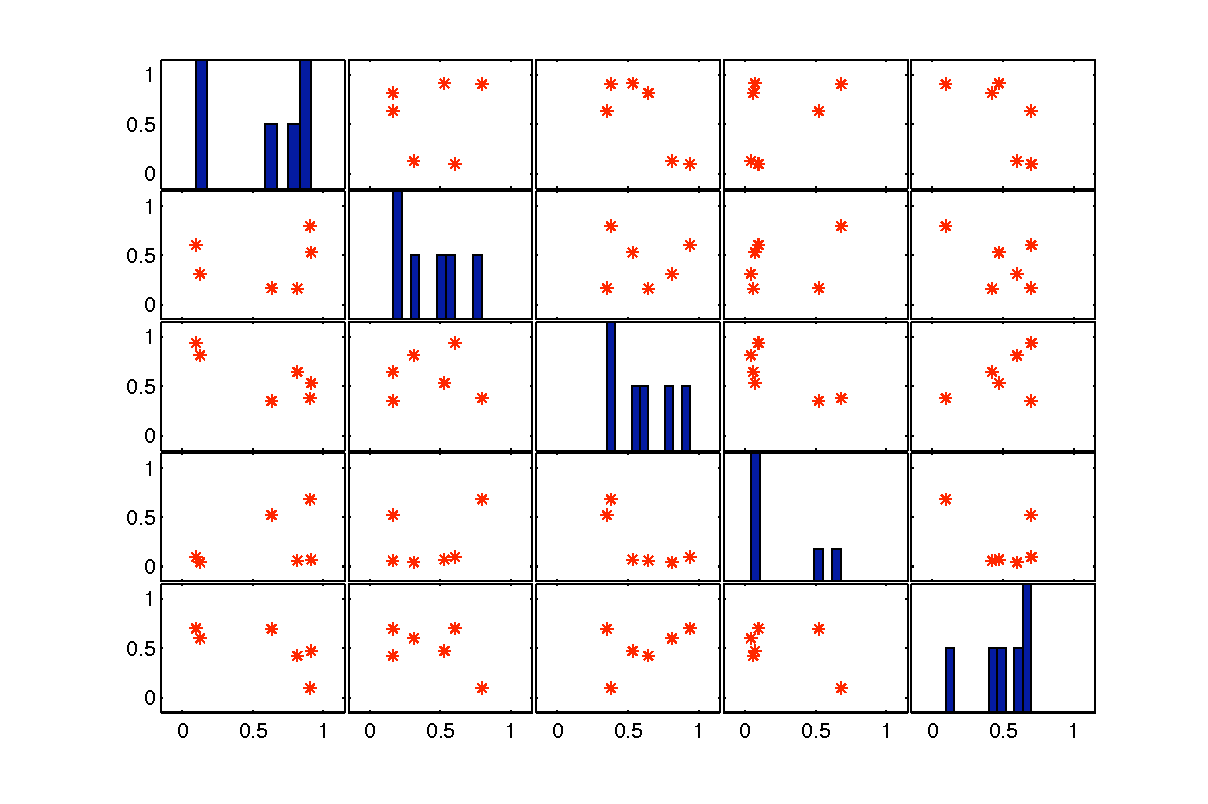
\includegraphics[width=3.750in]{figures/Twister5489X100x5PlotMatrixFirst6}} \hspace{-1.cm}
	   \subfigure[All thousand samples]{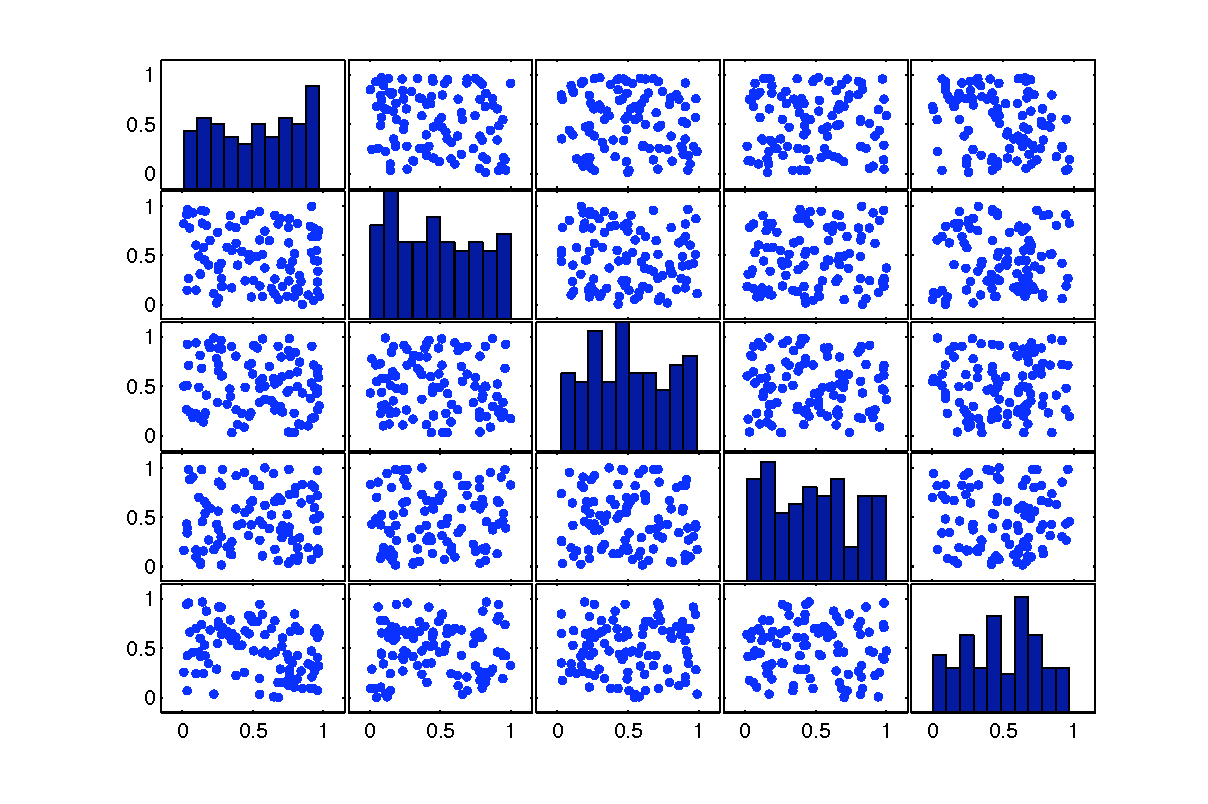
\includegraphics[width=3.750in]{figures/Twister5489X100x5PlotMatrixAll100}} }
\end{figure}

\begin{labwork}\label{LW:matrixplot5DUniform}
Let us make matrix plots from a uniformly generated  sequence of $100$ points in 5D unit cube $[0,1]^5$ as shown in \hyperref[F:Twister5489X100x5PlotMatrixFirst6andAll100]{Figure~\ref*{F:Twister5489X100x5PlotMatrixFirst6andAll100}}.
\begin{VrbM}
>> rand('twister',5489);
>> % generate a sequence of 1000 points uniformly distributed in 5D unit cube [0,1]X[0,1]X[0,1]X[0,1]X[0,1]
>> x=rand(1000,5);
>> x(1:6,:) % first six points in our 5D unit cube, i.e., the first six rows of x
ans =
    0.8147    0.6312    0.7449    0.3796    0.4271
    0.9058    0.3551    0.8923    0.3191    0.9554
    0.1270    0.9970    0.2426    0.9861    0.7242
    0.9134    0.2242    0.1296    0.7182    0.5809
    0.6324    0.6525    0.2251    0.4132    0.5403
    0.0975    0.6050    0.3500    0.0986    0.7054
>> plotmatrix(x(1:5,:),'r*') % make a plot matrix
>> plotmatrix(x) % make a plot matrix of all 1000 points
\end{VrbM}
\end{labwork}


\subsection{Loading and Exploring Real-world Data}\label{S:EDA}

All of the data we have played with so far were computer-generated.  It is time to get our hands dirty with real-world data.  The first step is to obtain the data.
Often, publicly-funded institutions allow the public to access their databases.  Such data can be fetched from appropriate URLs in one of the two following ways:
\begin{itemize}
\item[{\sf Method~A}:] Manually download by filling the appropriate fields in an online request form.
\item[{\sf Method~B}:] Automagically download directly from your \Matlab session.
\end{itemize}
Then we want to inspect it for inconsistencies, missing values and replace them with {\tt NaN} values in \Matlab that stand for not-any-number.  Finally, we can visually explore, transform and interact with the data to discover interesting patterns that are hidden in the data.  This process is called {\em exploratory data analysis} and is the foundational first step towards subsequent computational statistical experiments [{\em John W.~Tukey, Exploratory Data Analysis, Addison-Wesely, New York, 1977}].

\subsection{Geological Data}
 Let us focus on the data of earth quakes that heavily damaged Christchurch on February 22 2011.  This data can be fetched from the URL \href{http://magma.geonet.org.nz/resources/quakesearch/}{\url{http://magma.geonet.org.nz/resources/quakesearch/}} by {\sf Method A} and loaded into \Matlab for exploratory data analysis as done in \hyperref[LW:NZEQChCch20110222]{Labwork~\ref*{LW:NZEQChCch20110222}}.

 \begin{labwork}\label{LW:NZEQChCch20110222}
Let us go through the process one step at a time using {\sf Method~A}.
\begin{enumerate}
\item Download the data as a CSV or {\em comma separated variable} file in plain ASCII text (this has been done for this data already for you and saved as {\tt NZ20110222earthquakes.csv} in the {\tt CSEMatlabScripts} directory).
\item Open the file in a simple text editor such as {\tt Note Pad} in Windows or one of the following editors in OS X, Unix, Solaris, Linux/GNU variants such as Ubuntu, SUSE, etc: {\tt vi}, {\tt vim}, {\tt emacs}, {\tt geany}, etc.  The first three and last two lines of this file look as follows:
\begin{VrbM}
CUSP_ID,LAT,LONG,NZMGE,NZMGN,ORI_YEAR,ORI_MONTH,ORI_DAY,ORI_HOUR,ORI_MINUTE,ORI_SECOND,MAG,DEPTH
3481751,-43.55432,172.68898,2484890,5739375,2011,2,22,0,0,31.27814,3.79,5.8559,
3481760,-43.56579,172.70621,2486287,5738106,2011,2,22,0,0,43.70276,3.76,5.4045,
.
.
.
3469114,-43.58007,172.67126,2483470,5736509,2011,2,22,23,28,11.1014,3.117,3,
3469122,-43.55949,172.70396,2486103,5738805,2011,2,22,23,50,1.06171,3.136,12,
\end{VrbM}
The thirteen columns correspond to fairly self-descriptive features of each measured earth quake given in the first line or row.  They will become clear in the sequel.  Note that the comma character (`{\tt ,}') separates each unit or measurement or descpiption in any CSV file.

\item The next set of commands show you how to load,  manipulate and visually explore this data.

\begin{VrbM}
%% Load the data from the comma delimited text file 'NZ20110222earthquakes.csv' with
%% the following column IDs
%% CUSP_ID,LAT,LONG,NZMGE,NZMGN,ORI_YEAR,ORI_MONTH,ORI_DAY,ORI_HOUR,ORI_MINUTE,ORI_SECOND,MAG,DEPTH
%% Using MATLAB's dlmread command we can assign the data as a matrix to EQ;
%% note that the option 1,0 to dlmread skips first row of column descriptors
%
% the variable EQall is about to be assigned the data as a matrix
EQall = dlmread('NZ20110222earthquakes.csv', ',' , 1, 0);
size(EQall) % report the dimensions or size of the matrix EQall
ans =
   145    14
\end{VrbM}

\item In order to understand the syntax in detail get {\tt help} from \Matlab!
\begin{VrbM}
>> help dlmread
 DLMREAD Read ASCII delimited file.
 .
 .
 .
 \end{VrbM}

\item When there are units in the CSV file that can't be converted to floating-point numbers, it is customary to load them as a {\tt NaN} or {\em Not-a-Number} value in \Matlab.  So, let's check if there are any rows with {\tt NaN} values and remove them from our analysis.  Note that this is not the only way to deal with missing data! After that let's remove any locations outside Christchurch and its suburbs (we can find the latitude and longitude bounds from online resources easily) and finally view the 4-tuples of (latitude, longitude, magnitude, depth) for each measured earth quake in Christchurch on February 22 of 2011 as a scatter plot shown in \hyperref[F:NZEQ20110222ChchLtLnMgDpScatterMatrixPlot]{Figure~\ref*{F:NZEQ20110222ChchLtLnMgDpScatterMatrixPlot}} (the axes labels were subsequently added from clicking {\tt <Edit>} and {\tt <Figure Properties...>} tabs of the output Figure Window).
 \begin{VrbM}
>> EQall(any(isnan(EQall),2),:) = []; %Remove any rows containing NaNs from the matrix EQall
>> % report the size of EQall and see if it is different from before we removed and NaN containing rows
>> size(EQall)
ans =   145    14
>> % remove locations outside Chch and assign it to a new variable called EQ
>> EQ = EQall(-43.75<EQall(:,2) & EQall(:,2)<-43.45 ...
              & 172.45<EQall(:,3) & EQall(:,3)<172.9 & EQall(:,12)>3, :);
>> % now report the size of the earthquakes in Christchurch in variable EQ
>> size(EQ)
ans =   124    14
>> % assign the four variables of interest
>> LatData=EQ(:,2); LonData=EQ(:,3); MagData=EQ(:,12); DepData=EQ(:,13);
>> % finally make a plot matrix of these 124 4-tuples as red points
>> plotmatrix([LatData,LonData,MagData,DepData], 'r.');
\end{VrbM}
\end{enumerate}
All of these commands have been put in a script M-file {\tt NZEQChCch20110222.m} %in \hyperref[Mf:NZEQChCch20110222]{Labwork~\ref*{Mf:NZEQChCch20110222}}
and you can simply call it from the command window to automatically load the data and assign it to the variables {\tt EQAll} {\tt EQ}, {\tt LatData}, {\tt LonData}, {\tt MagData} and {\tt DepData}, instead of retyping each command above every time you need these matrices in \Matlab, as follows:
\begin{VrbM}
>> NZEQChCch20110222
ans =   145    14
ans =   145    14
ans =   124    14
\end{VrbM}
In fact, we will do exactly this to conduct more exploratory data analysis with these earth quake measurements in \hyperref[LW:NZEQChCch20110222EDA]{Labwork~\ref*{LW:NZEQChCch20110222EDA}}.
\end{labwork}

\begin{figure}[htpb]
\caption{Matrix of Scatter Plots of the latitude, longitude, magnitude and depth of the 22-02-2011 earth quakes in Christchurch, New Zealand.\label{F:NZEQ20110222ChchLtLnMgDpScatterMatrixPlot}}
\centering   \makebox{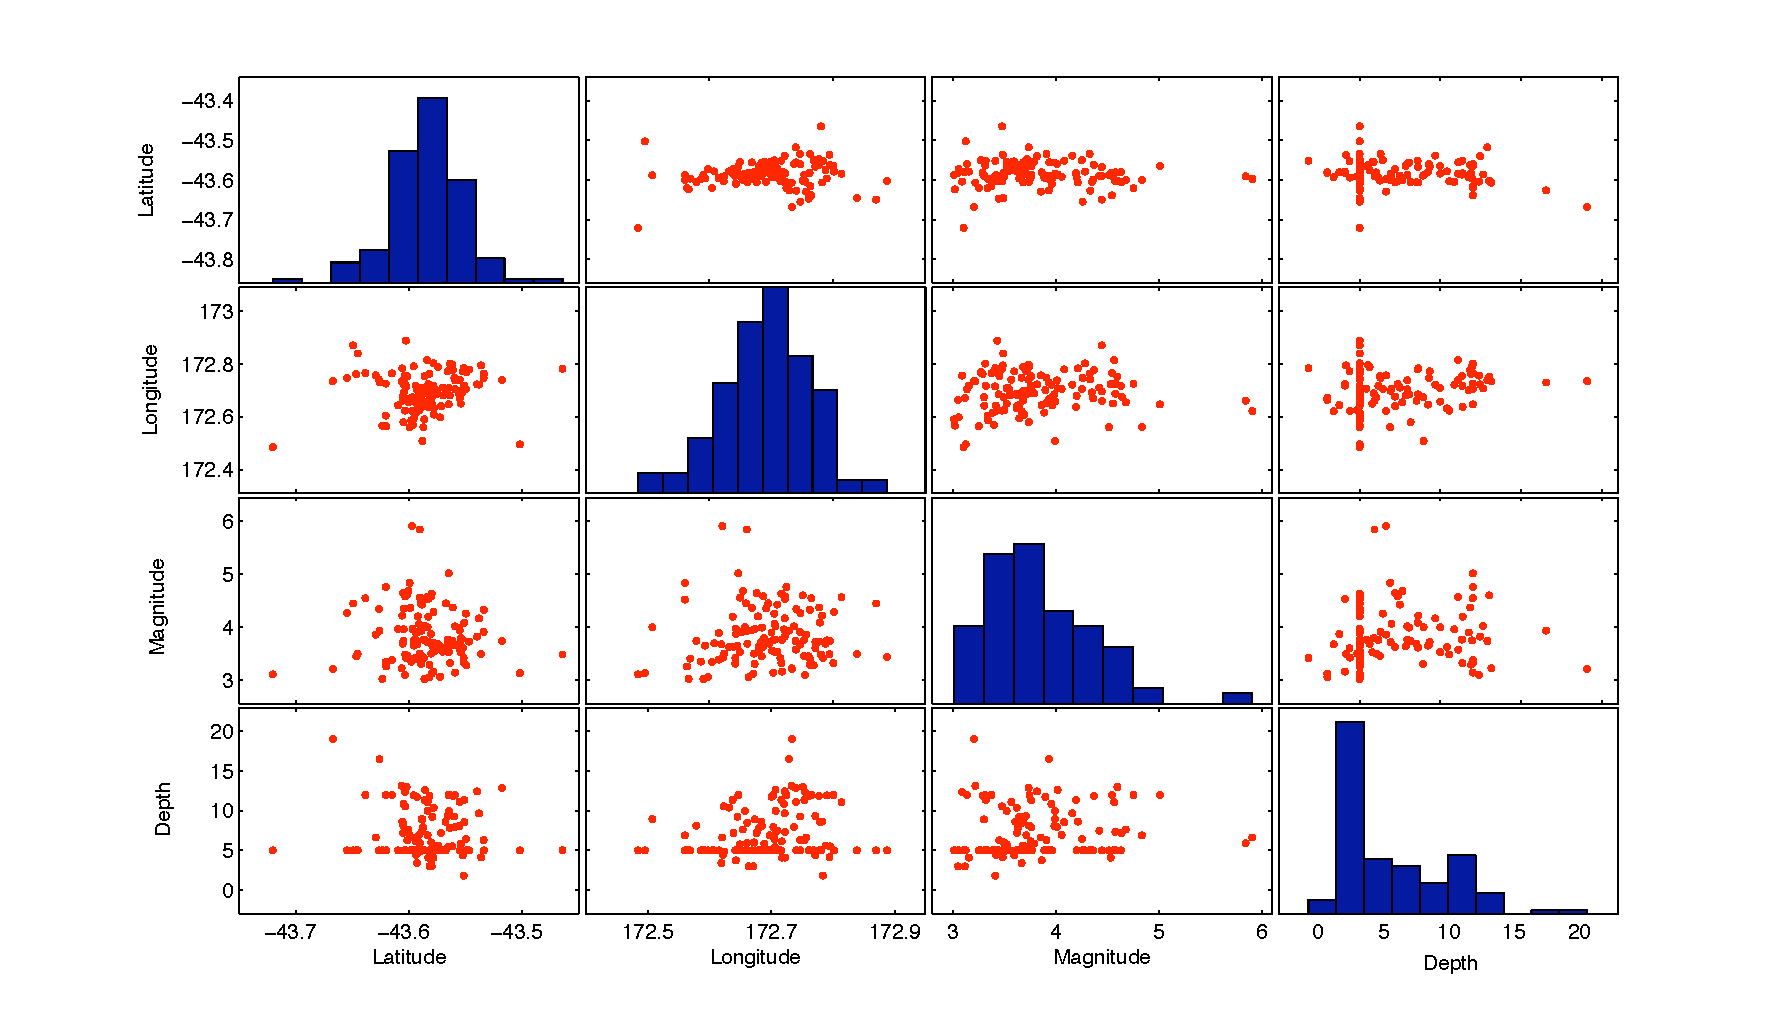
\includegraphics[width=6.5in]{figures/NZEQ20110222ChchLtLnMgDpScatterMatrixPlot}}
\end{figure}


\begin{labwork}\label{LW:NZEQChCch20110222EDA}
Try to understand how to manipulate time stamps of events in \Matlab and the Figures being output by following the comments in the script file {\tt NZEQChCch20110222EDA.m}.
\begin{VrbM}
>> NZEQChCch20110222
ans =   145    14
ans =   145    14
ans =   124    14
ans =   145    14
ans =   145    14
ans =   124    14
ans = 22-Feb-2011 00:00:31
ans = 22-Feb-2011 23:50:01
\end{VrbM}
\VrbMf[label=NZEQChCch20110222EDA.m]{scripts/NZEQChCch20110222EDA.m}
\end{labwork}

\subsubsection{Geostatistical exploratory data analysis with Google Earth}

\begin{figure}[htpb]
\caption{Google Earth Visualisation of the earth quakes\label{F:NZEQ20110222ChchLtLnMgDpInGoogleEarthViewFromUSGS}}
\centering   \makebox{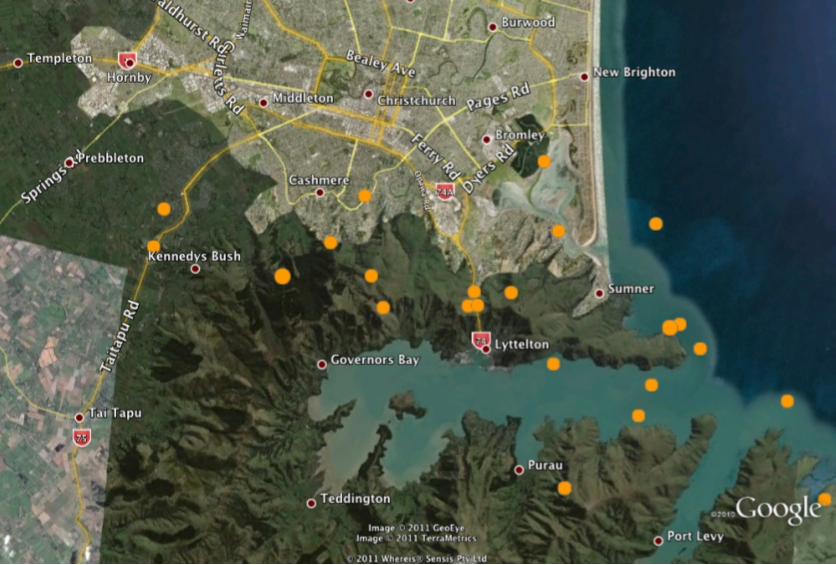
\includegraphics[width=4.5in]{figures/NZEQ20110222ChchLtLnMgDpInGoogleEarthViewFromUSGS}}
\end{figure}

A global search at \href{http://neic.usgs.gov/cgi-bin/epic/epic.cgi}{\url{http://neic.usgs.gov/cgi-bin/epic/epic.cgi}}
%%?SEARCHMETHOD=1&FILEFORMAT=7&SEARCHRANGE=PP&SYEAR=2011&SMONTH=2&SDAY=22&EYEAR=2011&EMONTH=2&EDAY=22&LMAG=&UMAG=&NDEP1=&NDEP2=&IO1=&IO2=&CLAT=0.0&CLON=0.0&CRAD=0.0&SUBMIT=Submit+Search}
with the following parameters:
\begin{verbatim}
Date Range: 2011 2 22 to 2011 2 22
Catalog: USGS/NEIC (PDE-Q)
\end{verbatim}
produced 43 earth quakes world-wide, including those in Christchurch as shown in \hyperref[F:NZEQ20110222ChchLtLnMgDpInGoogleEarthViewFromUSGS]{Figure~\ref*{F:NZEQ20110222ChchLtLnMgDpInGoogleEarthViewFromUSGS}}.  One can do a lot more than a mere visualisation with the USGS/NEIC  database of earth-quakes wolrd-wide, the freely available {\tt Google earth} software bundle \href{http://www.google.com/earth/index.html}{\url{http://www.google.com/earth/index.html}} and the freely available \Matlab package {\tt googleearth} from \href{http://www.mathworks.com/matlabcentral/fx_files/12954/4/content/googleearth/html/html_product_page.html}{\url{http://www.mathworks.com/matlabcentral/fx_files/12954/4/content/googleearth/html/html_product_page.html}}.

\subsection{Metereological Data}

New Zealand's meteorological service NIWA provides weather data under it TERMS AND CONDITIONS FOR ACCESS TO DATA (See \url{http://cliflo.niwa.co.nz/doc/terms_print.html}).  We will explore some data of rainfall and temperatures from NIWA.

\subsubsection{Daily Rainfalls in Christchurch}

%Rainfall Data in Christchurch

Automagic downloading of the data by {\sf Method B} can be done if the data provider allows automated queries.  It can be accomplished by {\tt urlread} for instance.  %Try to download the file



%is being  \work.  But you can t

Paul Brouwers has a basic CliFlo datafeed on \url{http://www.math.canterbury.ac.nz/php/lib/cliflo/rainfall.php}.  %?range=20100425:20100501
This returns the date and rainfall in milli meters as measured from the CHCH aeroclub station. It is assumed that days without readings would not be listed. %It expects a range parameter such as: ?range=20100425:20100501 The first number is the starting search date (YYYYMMDD). Colon as separator. The first number is the ending search date (YYYYMMDD). CliFlo limits us to 2 million rows for the subscription and 40,000 rows per query (which is equivalent of over 100 years of data, so I we're safe -
The data doesn't go back much before 1944.

%wetdataURL = 'http://www.math.canterbury.ac.nz/php/lib/cliflo/?range=20100101:20100510' wetdataURL = 'http://www.math.canterbury.ac.nz/php/lib/cliflo/rainfall.php'
%\work


\begin{labwork}\label{LW:ChchDailyRainfallSince}
Understand how \hyperref[F:ChchDailyRainfallSince]{Figure~\ref*{F:ChchDailyRainfallSince}} is obtained by the script file {\tt RainFallsInChch.m} by typing and following the comments:

\begin{VrbM}
>> RainFallsInChch
RainFallsChch =     [24312x1 int32]    [24312x1 double]
ans =       24312           2
FirstDayOfData =    19430802
LastDayOfData =    20100721
\end{VrbM}

\VrbMf[label=RainFallsInChch.m]{scripts/RainFallsInChch.m}
\end{labwork}

\begin{figure}[htpb]
\caption{Daily rainfalls in Christchurch since March 27 2010 \label{F:ChchDailyRainfallSince}}
\centering   \makebox{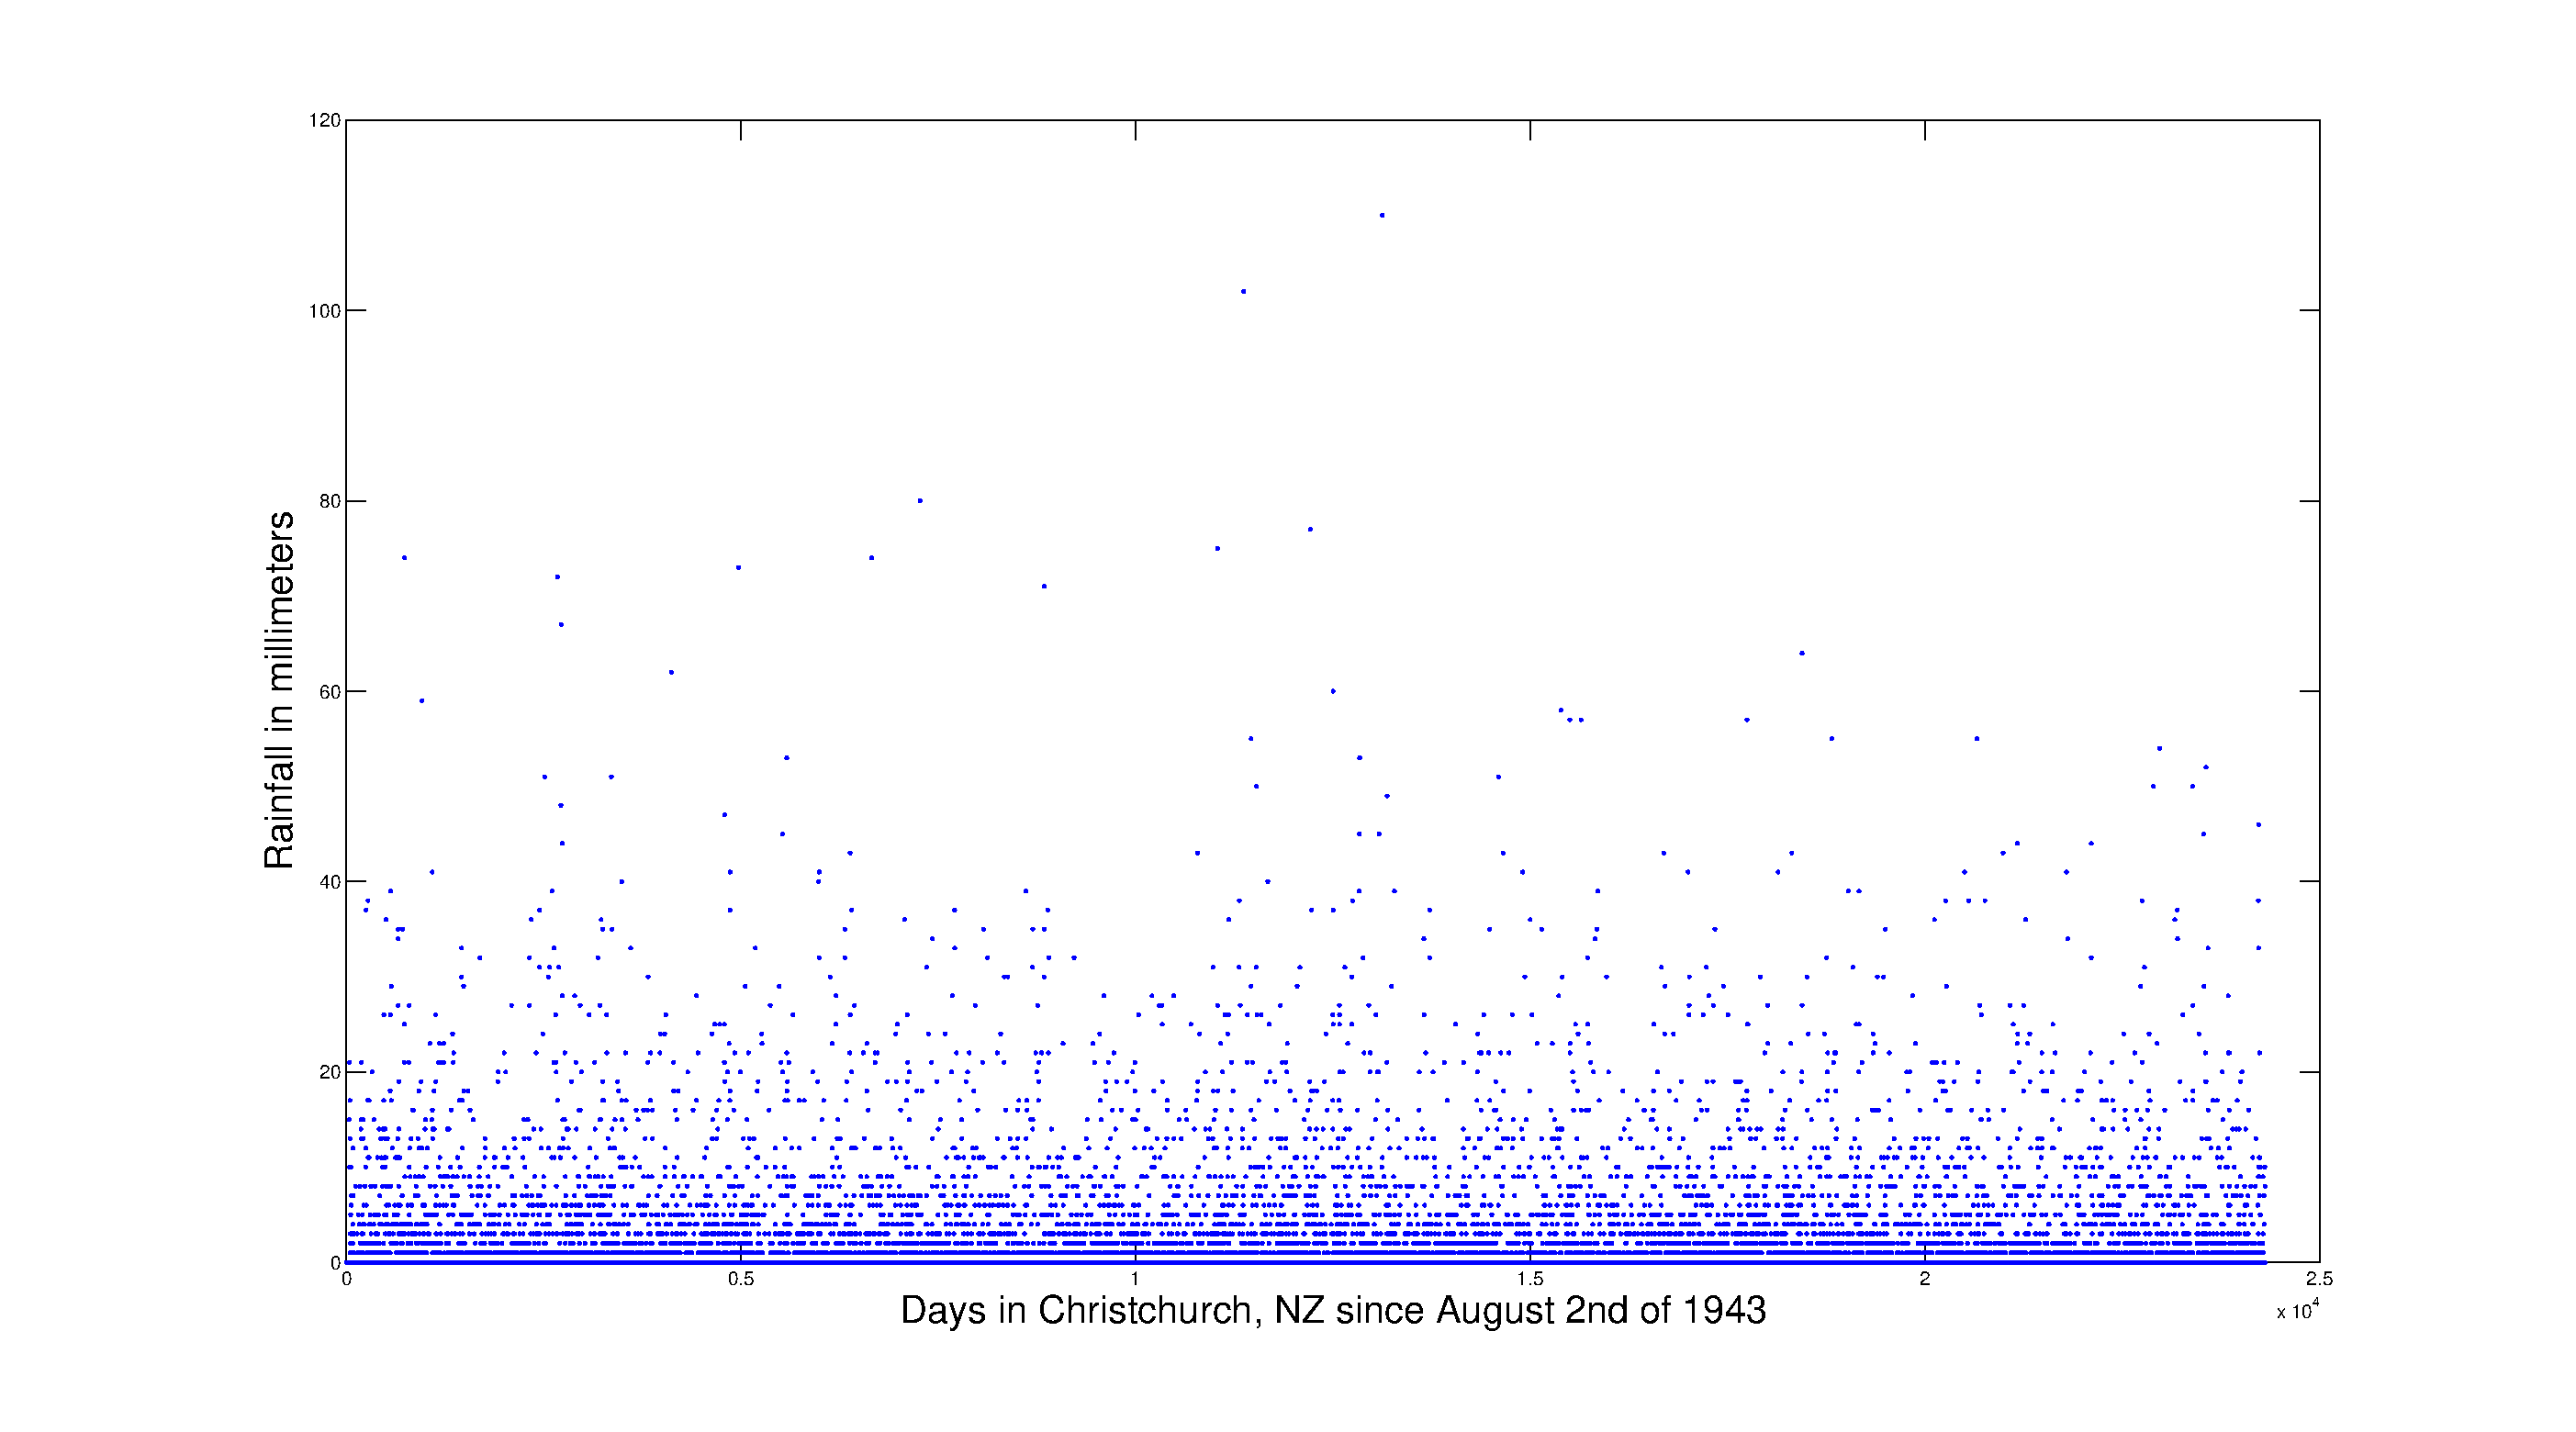
\includegraphics[width=6.5in]{figures/ChchDailyRainfallSince}}
\end{figure}

\subsubsection{Daily Temperatures in Christchurch}


\begin{labwork}\label{LW:ChchTempsLoad}
Understand how \hyperref[F:ChchTemps365DaysSince20100327]{Figure~\ref*{F:ChchTemps365DaysSince20100327}} is being generated by following the comments in the script file {\tt ChchTempsLoad.m} by typing:
\begin{VrbM}
>> ChchTempsLoad
\end{VrbM}
\VrbMf[label=ChchTempsLoad.m]{scripts/ChchTempsLoad.m}
\end{labwork}

\begin{figure}[htpb]
\caption{Daily temperatures in Christchurch for one year since March 27 2010 \label{F:ChchTemps365DaysSince20100327}}
\centering   \makebox{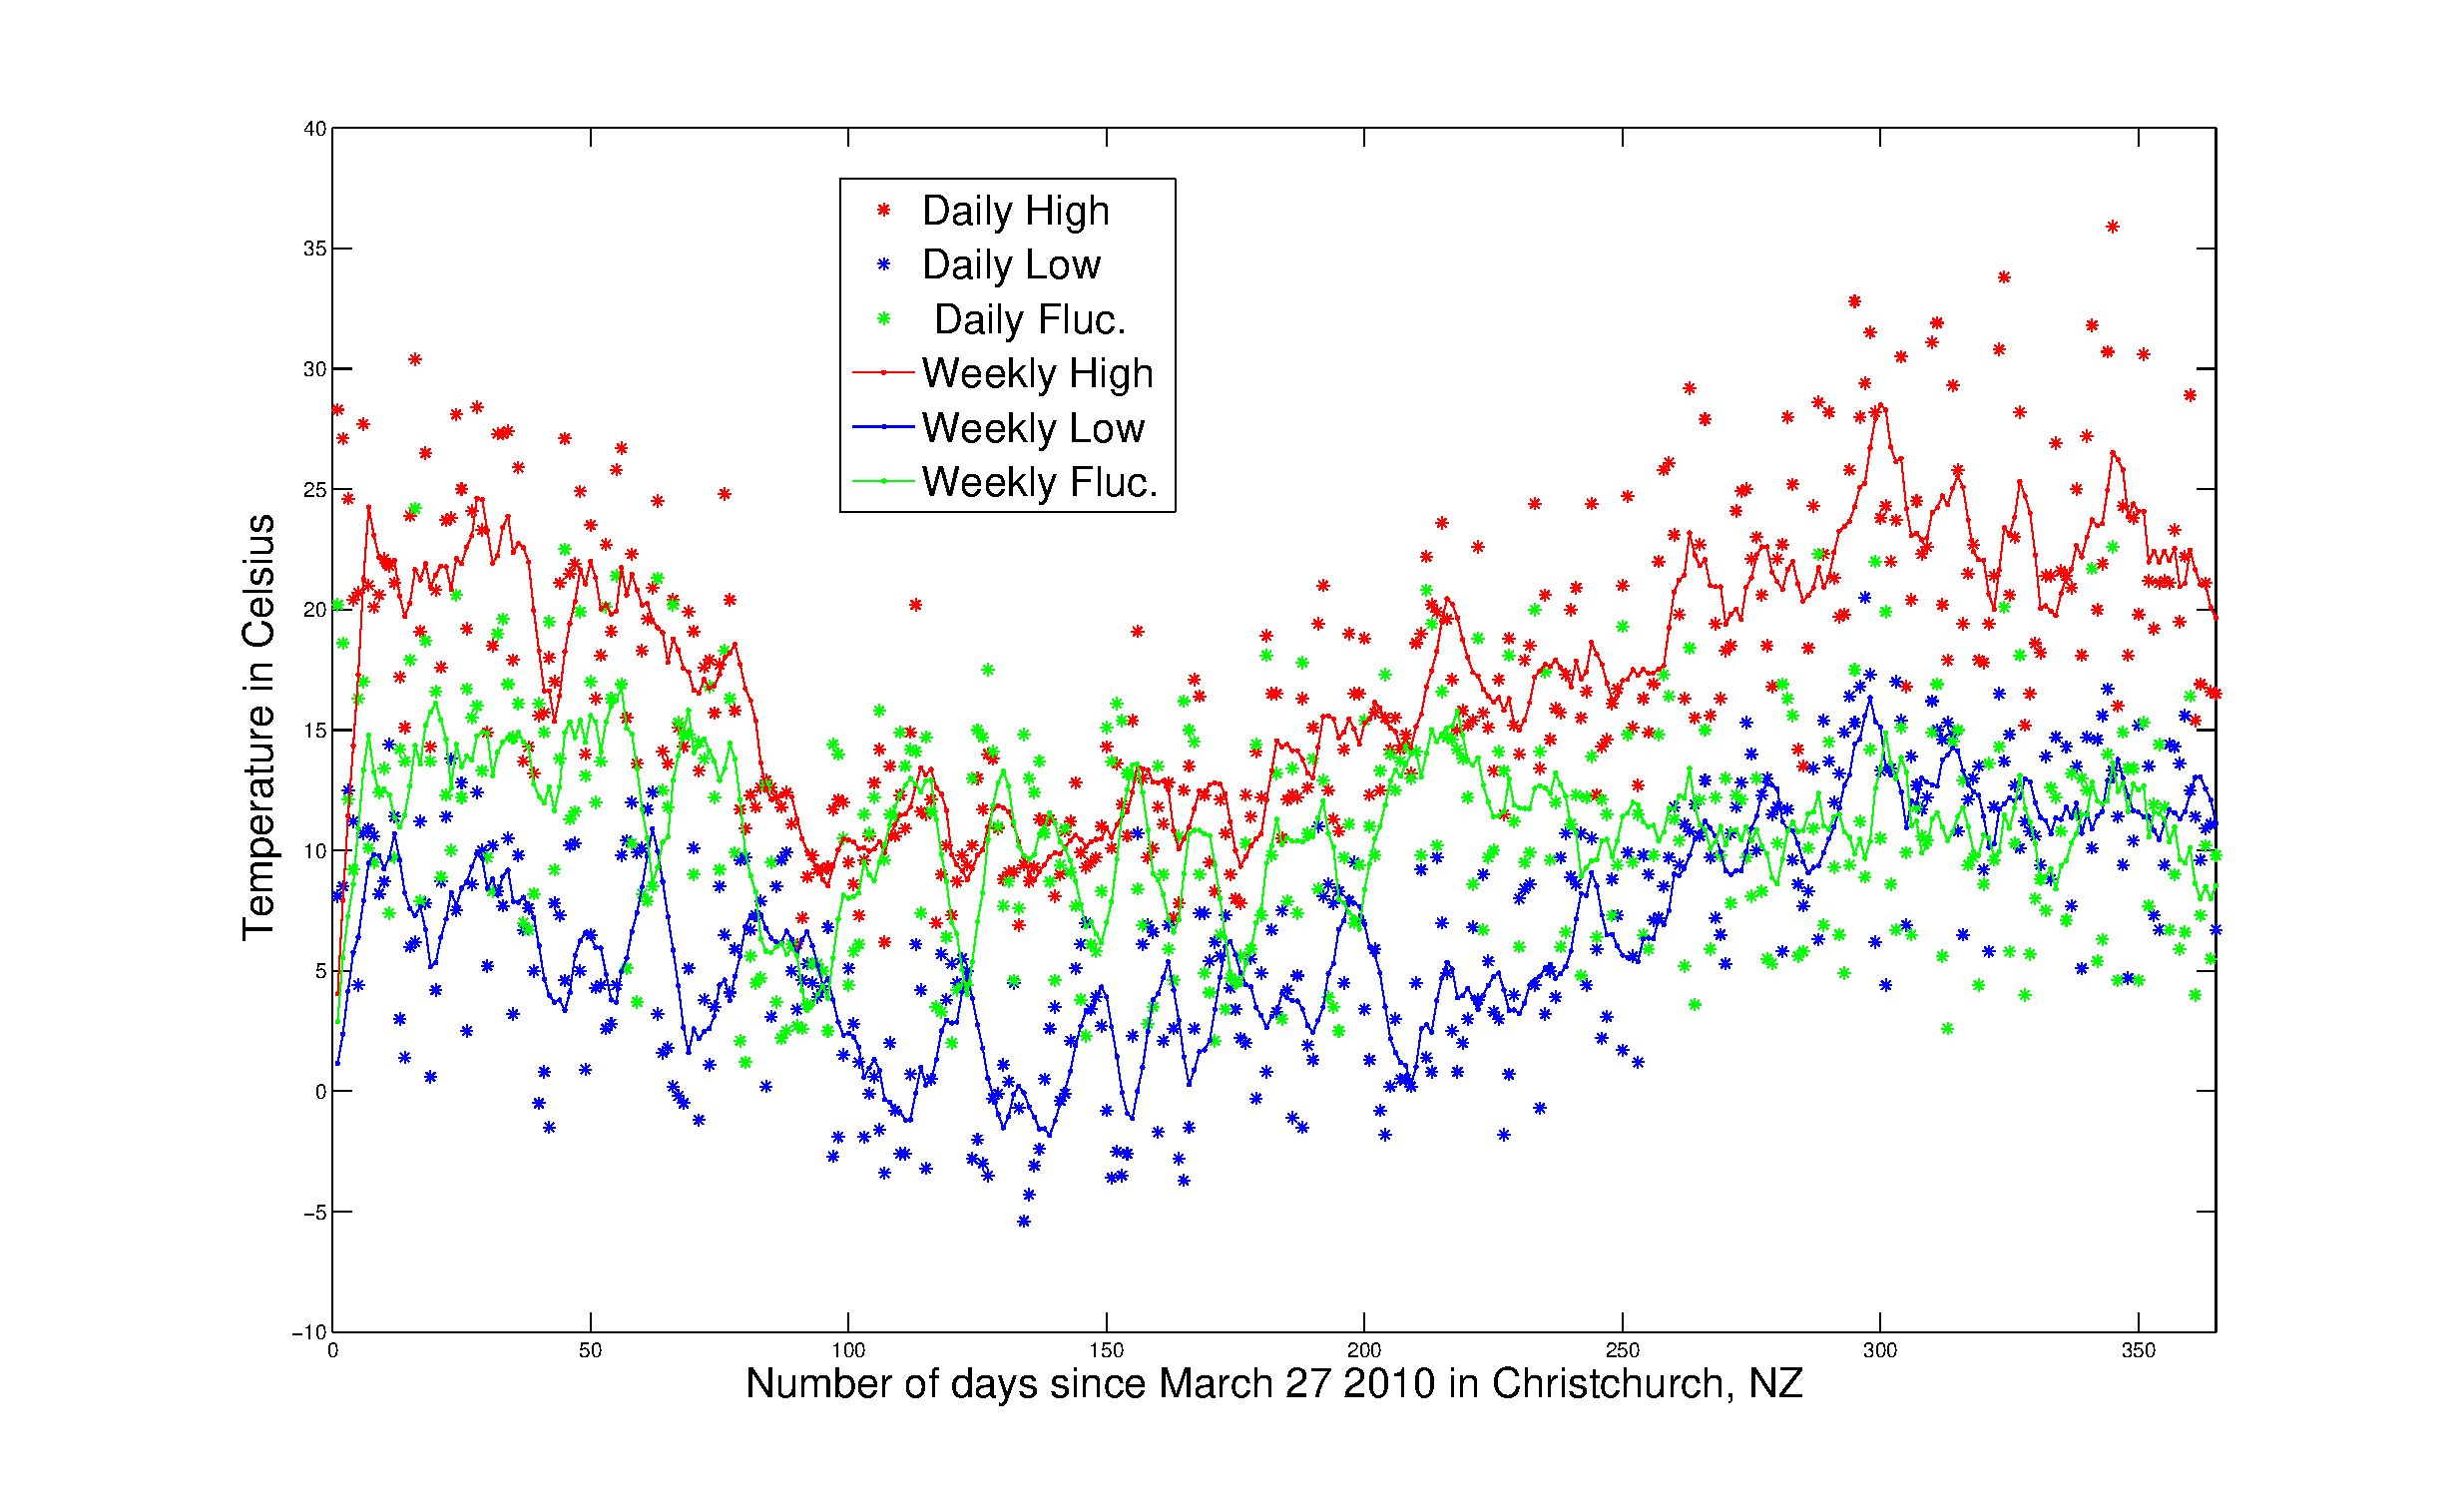
\includegraphics[width=6.5in]{figures/ChchTemps365DaysSince20100327}}
\end{figure}

\subsection{Textual Data}

Processing and analysing textual data to make a decision is another important computational statistical experiment. An obvious example  is machine translation and a less obvious one is exploratory data analysis of the textual content of
\begin{itemize}
\item a large document
\item twitter messages within an online social network of interest
\item etc.
\end{itemize}

An interesting document with a current affairs projection is the Joint Operating Environment 2010 Report by the US Department of Defense.  This document was downloaded from \href{http://www.jfcom.mil/newslink/storyarchive/2010/JOE_2010_o.pdf}{\url{http://www.jfcom.mil/newslink/storyarchive/2010/JOE_2010_o.pdf}}.  The first paragraph of this 74 page document (JOE 2010 Reprort) reads:

{\small
ABOUT THIS STUDY The Joint Operating Environment is intended to inform joint concept development and experimentation throughout the Department of Defense. It provides a perspective on future trends, shocks, contexts, and implications for future joint force commanders and other leaders and professionals in the national security field. This document is speculative in nature and does not suppose to predict what will happen in the next twenty-five years. Rather, it is intended to serve as a starting point for discussions about the future security environment at the operational level of war. Inquiries about the Joint Operating Environment should be directed to USJFCOM Public Affairs, 1562 Mitscher Avenue, Suite 200, Norfolk, VA 23551-2488, (757) 836-6555.

Distribution Statement A: Approved for Public Release
}

\begin{figure}[htpb]
\caption{Wordle of JOE 2010\label{F:joe_vs_wordle}}
\centering   \makebox{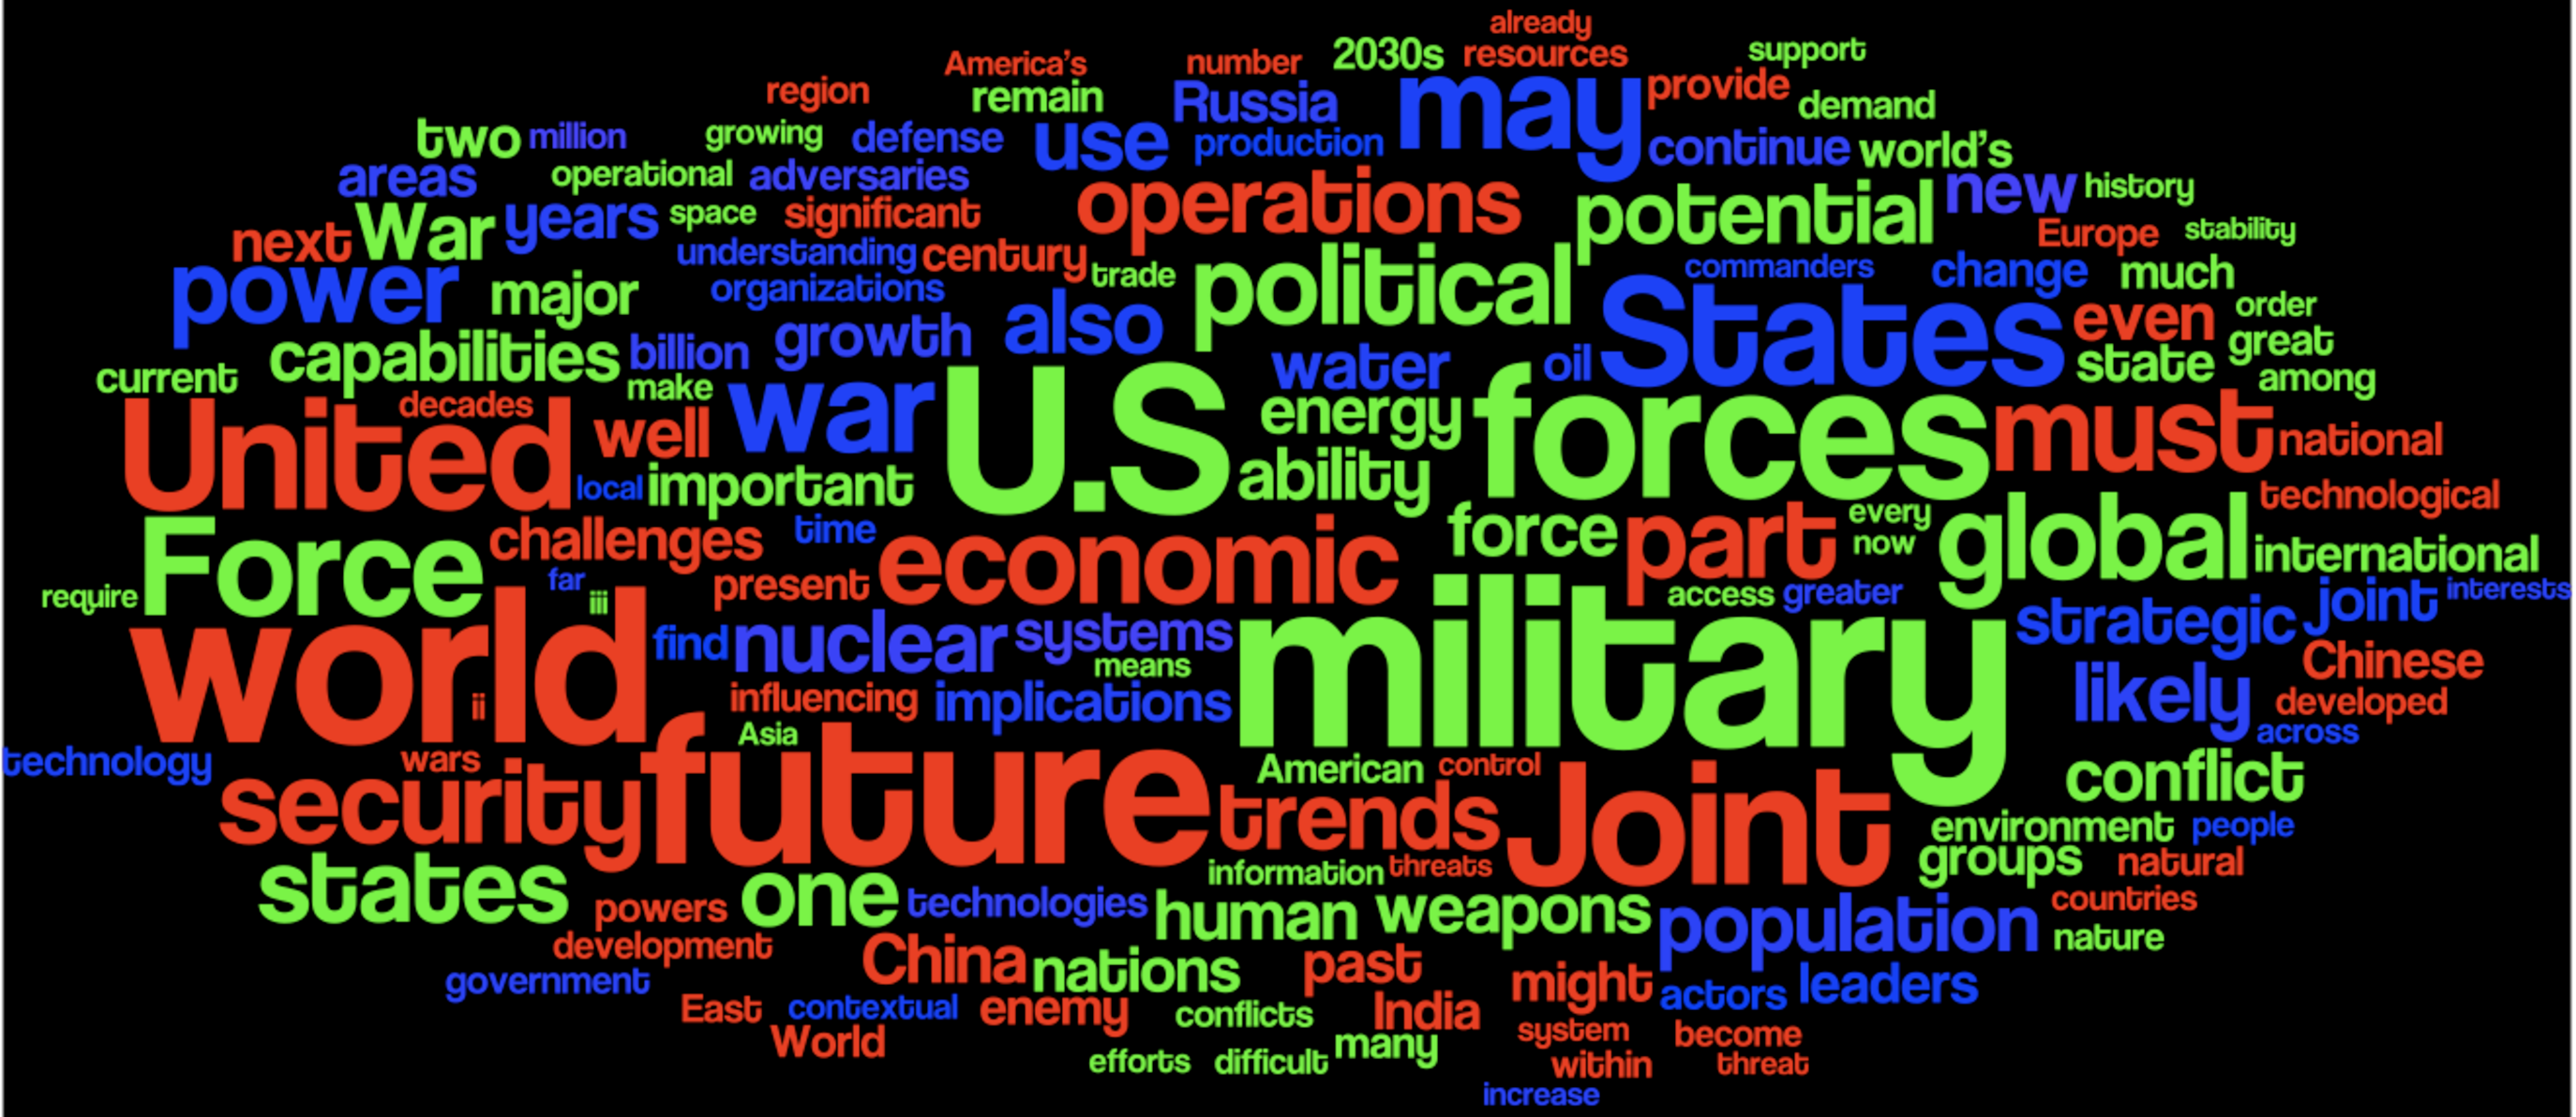
\includegraphics[width=6.5in]{figures/joe_vs_wordle_RaazCroppedPhilWilsonsImage}}
\end{figure}

We can try to produce a statistic of this document by recording the frequency of words in its textual content. Then we can produce a ``word histogram'' or ``word cloud'' to explore the document visually at one of the coarsest possible resolutions of the textual content in the JOE 2010 Report.  The ``word cloud'' shown in \hyperref[F:joe_vs_wordle]{Figure~\ref*{F:joe_vs_wordle}} was produced by Phillip Wilson using {\em wordle} from \href{http://www.wordle.net/}{\url{http://www.wordle.net/}}.  A description from the wordle URL says:

{\small
Wordle is a toy for generating Òword cloudsÓ from text that you provide. The clouds give greater prominence to words that appear more frequently in the source text. You can tweak your clouds with different fonts, layouts, and color schemes. The images you create with Wordle are yours to use however you like. You can print them out, or save them to the Wordle gallery to share with your friends.
}

\begin{labwork}[favourite word cloud]\label{LW:JoeWordle}  This is just for fun.  Produce a ``word cloud'' of your honours thesis or summer project or any other document that fancies your interest by using {\em wordle} from \href{http://www.wordle.net/}{\url{http://www.wordle.net/}}. Play with the aesthetic features to change colour, shapes, etc.\end{labwork}

\subsection{Machine Sensor Data}

Instrumentation of modern machines, such as planes, rockets and cars allow the sensors in the machines to collect live data and dynamically take {\em decisions} and subsequent {\em actions} by executing algorithms to drive their devices in response to the data that is streaming into their sensors.  For example, a rocket may have to adjust its boosters to compensate for the prevailing directional changes in wind in order to keep going up and launch a satellite.
These types of decisions and actions, theorised by {\em controlled Markov processes}, typically arise in various fields of engineering such as, aerospace, civil, electrical, mechanical, robotics, etc.

In an observational setting, without an associated control problem, one can use machine sensor data to get information about some state of the system or phenomenon, i.e., what is it doing? or where is it?, etc.  Sometimes sensors are attached to a sample of individuals from a  wild population, say Emperor Penguins in Antarctica where the phenomenon of interest may be the diving habits of this species after the eggs hatch.  As an other example we can attach sensors to a double pendulum and find what it is doing when we give it a spin.

Based on such observational data the experimenter typically tries to learn about the behaviour of the system from the sensor data to estimate parameters, test hypotheses, etc. Such types of experiments are typically performed by scientists in various fields of science, such as, astronomy, biology, chemistry, geology, physics, etc.

\subsubsection{Chaotic Time Series of a Double Pendulum}

\begin{figure}[htbp]
\begin{center}
{\scriptsize
\begin{tabular}{ccc}
A: DP Schematic & B: Streaming DP data & C: Enclosures of two initially close trajectories\\
  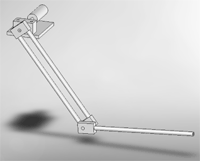
\includegraphics[scale=0.5]{figures/dp} &
  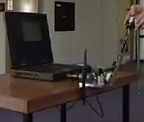
\includegraphics[scale=0.66]{figures/vlcsnap-2010-01-13-10h11m08s38_closeup} &
  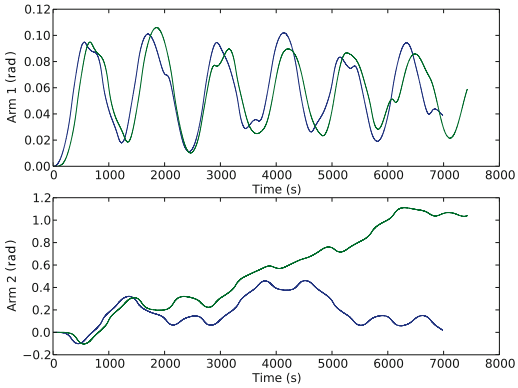
\includegraphics[height=3cm,width=6.75cm]{figures/divergence_piers}
\end{tabular}
}
\end{center}
\caption{Double Pendulum}
\label{F:DP3}
\end{figure}

Sensors called {\em optical encoders} have been attached to the top end of each arm of a chaotic double pendulum in order to obtain the angular position of each arm through time as shown in \hyperref[F:DP3]{Figure~\ref*{F:DP3}}.  Time series of the angular position of each arm for two trajectories that were initialized very similarly, say the angles of each arm of the double pendulum are almost the same at the initial time of release.  Note how quickly the two trajectories diverge!  System with such a sensitivity to initial conditions are said to be {\em chaotic}.

\begin{labwork}[A Challenging Task]\label{LW:DPtrajectoryparsing}  Try this if you are interested.  Read any of the needed details about the design and fabrication of  the double pendulum at \href{http://www.math.canterbury.ac.nz/~r.sainudiin/lmse/double-pendulum/}{\url{http://www.math.canterbury.ac.nz/~r.sainudiin/lmse/double-pendulum/}}.  Then use \Matlab to generate a plot similar to \hyperref[F:DP3]{Figure~\ref*{F:DP3}(C)} using time series data of {\sf trajectory~1} and {\sf  trajectory~2} linked from the bottom of the above URL.
 \end{labwork}

\comment{
\subsection{Biological Data}
\work
}

\section{Exercises in Statistics}\label{S:xsStatistics}
\begin{ExerciseList}
\Exercise What is the sample mean and sample variance of the following dataset:
\[
1, 3, 2, 1, 2, 3, 3
\]
\Answer Apply the formulas for the sample mean, $\overline{X_7}$, and sample variance.
\end{ExerciseList}



%\remove
%%%%%%%%%%%%%%%%%%%%%%%%%%%%%%%%%%%%%%%%%%%%%%%%%%%%%%%%%%%%%%%%%%%%%%%%%%%%%%
%%%% snipped above into csebook

\chapter{Fundamentals of Estimation}
\section{Introduction}
Now that we have been introduced to two notions of convergence for RV sequences, we can begin to appreciate the basic limit theorems used in statistical inference.  The problem of estimation is of fundamental importance in statistical inference and learning.  We will formalise the general estimation problem here.  There are two basic types of estimation.  In point estimation we are interested in estimating a particular point of interest that is supposed to belong to a set of points.  In (confidence) set estimation, we are interested in estimating a set with a particular form that has a specified probability of ``trapping'' the particular point of interest from a set of points.  Here, a point should be interpreted as an element of a collection of elements from some space.

\section{Point Estimation}\label{S:PointEstimation}
{\bf Point estimation} is any statistical methodology that provides one with a ``{\bf single best guess}'' of some specific quantity of interest.  Traditionally, we denote this {\bf quantity of interest as $\theta^*$} and {\bf its point estimate as $\widehat{\theta}$ or $\widehat{\theta}_n$}.  The subscript $n$ in the point estimate $\widehat{\theta}_n$ emphasises that our estimate is based on $n$ observations or data points from a given statistical experiment to estimate $\theta^*$.  This quantity of interest, which is usually unknown, can be: %, namely $\theta$
%, may be an {\bf integral} $\Iz$ of a real valued function $h(x)$, i.e.~$\theta=\Iz := \int_a^b h(x)\,dx \in \Rz$, or simply a 
\begin{itemize}
\item an {\bf integral} $\vartheta^* := \int_A h(x)\,dx \in \BB{\varTheta}$.  If $\vartheta^*$ is finite, then $\BB{\varTheta} =  \Rz$, or %  For e.g.~see \ref{S:BMC} on Monte Carlo integration.
\item a {\bf parameter} $\theta^*$ which is an element of the {\bf parameter space} $\BB{\Theta}$, denoted $\theta^* \in \BB{\Theta}$,
\item a {\bf distribution function (DF)} $F^* \in \Fz := \text{the set of all DFs}$
\item a {\bf density function (pdf)} $f \in \{ \text{``not too wiggly Sobolev functions''} \}$, or 
\item a {\bf regression function} $g^* \in \Gz$, where $\Gz$ is a class of regression functions in a regression experiment with model: $Y=g^*(X)+\epsilon$, such that $\E(\epsilon)=0$, from pairs of observations $\{(X_i,Y_i)\}_{i=1}^n$, or
\item a {\bf classifier} $g^* \in \Gz$, i.e.~a regression experiment with discrete $Y = g^*(X)+\epsilon$, or 
\item a {\bf prediction} in a regression experiment, i.e.~when you want to estimate $Y_i$ given $X_i$. 
\end{itemize}
%\begin{table}[htpb]
%\begin{center}
%\begin{tabular}{|c c c|}
%\hline
%Quantity of Interest $\theta$ & Point Estimation & Sections \\ \hline
%Parameter $\theta \in \BB{\Theta} \subset \Rz^n$ & Parametric Estimation & Section~\ref*{S:ParametricEstimation} \\
%Integral $\Iz := \int_a^bh(x)\,dx$ & Monte Carlo Integration & Section~\ref*{S:BMC} \\ \hline
%\end{tabular}
%\end{center}
%\end{table}

Recall that a statistic is an RV $T(X)$ that maps every data point $x$ in the data space $\Xz$ with $T(x)=t$ in its range $\Tz$, i.e.~$T(x):\Xz \to \Tz$ (\hyperref[D:Statistic]{Definition~\ref*{D:Statistic}}).  Next, we look at a specific class of statistics whose range is the parameter space $\BB{\Theta}$.
\begin{definition}[Point Estimator]\label{D:Estimator}
A {\bf point estimator} $\widehat{\Theta}$ of some {\bf fixed and possibly unknown} $\theta^* \in \BB{\Theta}$ is a statistic that associates each data point $x \in \Xz$ with an estimate $\widehat{\Theta}(x)=\widehat{\theta} \in \BB{\Theta}$,  
\[
\boxed{
 \widehat{\Theta} := \widehat{\Theta}(x)=\widehat{\theta}: \Xz \to \BB{\Theta}
 } \ .
\]
If our data point $x := (x_1,x_2,\ldots,x_n)$ is an $n$-vector or a point in the $n$-dimensional real space, i.e.~$x := (x_1,x_2,\ldots,x_n) \in \Xz_n \subset \Rz^n$, then we emphasise the dimension $n$ in our point estimator $\widehat{\Theta}_n$ of $\theta^* \in \BB{\Theta}$.
\[
\boxed{
\widehat{\Theta}_n :=  \widehat{\Theta}_n(x:=(x_1,x_2,\ldots,x_n))=\widehat{\theta}_n : \Xz_n \to \BB{\Theta}, \quad \Xz_n \subset \Rz^n 
} \ .
\]
 The typical situation for us involves point estimation of $\theta^* \in \BB{\Theta}$ on the basis of one realisation $x \in\Xz_n \subset \Rz^n$ of an independent and identically distributed (IID) random vector $X=(X_1,X_2,\ldots,X_n)$, such that $X_1,X_2,\ldots,X_n \overset{\IID}{\sim} X_1$ and the DF of $X_1$ is $F(x_1; \theta^*)$, i.e.~the distribution of the IID RVs, $X_1, X_2,\ldots,X_n$, is parameterised by $\theta^* \in \BB{\Theta}$.
\end{definition}

\begin{example}[Coin Tossing Experiment ($X_1,\ldots,X_n \overset{IID}{\sim} \bernoulli(\theta^*)$)]\label{EX:CoinTossing}
I tossed a coin that has an unknown probability $\theta^*$ of landing Heads independently and identically $10$ times in a row.  Four of my outcomes were Heads and the remaining six were Tails, with the actual sequence of Bernoulli outcomes (Heads $\to 1$ and Tails $\to 0$) being $(1,0,0,0,1,1,0,0,1,0)$.  I would like to estimate the probability $\theta^* \in \BB{\Theta} = [0,1]$ of observing Heads using the natural estimator $\widehat{\Theta}_n((X_1,X_2,\ldots,X_n))$ of $\theta^*$:
\[
\widehat{\Theta}_n((X_1,X_2,\ldots,X_n)) := \widehat{\Theta}_n = \frac{1}{n} \sum_{i=1}^n X_i =: \overline{X}_n
\]
For the coin tossing experiment I just performed ($n=10$ times), the point estimate of the unknown $\theta^*$ is:
\begin{eqnarray}
\widehat{\theta}_{10} = \widehat{\Theta}_{10}((x_1,x_2,\ldots,x_{10})) 
&=&\widehat{\Theta}_{10}((1,0,0,0,1,1,0,0,1,0)) \notag \\
&=& \frac{1+0+0+0+1+1+0+0+1+0}{10}=\frac{4}{10}=0.40 \notag \ .
\end{eqnarray}
\end{example}

\begin{labwork}[$\bernoulli(38/75)$ Computer Experiment]\label{LW:1000CoinTossingExp}
Simulate one thousand IID samples from a $\bernoulli(\theta^*=38/75)$ RV and store this data in an array called $\tt Samples$.  Use your student ID to initialise the fundamental sampler.  Now, pretend that you don't know the true $\theta^*$ and estimate $\theta^*$ using our estimator $\widehat{\Theta}_n=\overline{X}_n$ from the data array $\tt Samples$ for each sample size $n=1,2,\ldots,1000$.  Plot the one thousand estimates $\widehat{\theta}_1,\widehat{\theta}_2,\ldots,\widehat{\theta}_{1000}$ as a function of the corresponding sample size.  Report your observations regarding the behaviour of our estimator as the sample size increases.
\end{labwork}

\section{Some Properties of Point Estimators}\label{S:PropPointEstim}
Given that an estimator is merely a function from the data space to the parameter space, we need choose only the best estimators available.  Recall that a point estimator $\widehat{\Theta}_n$, being a statistic or an RV of the data has a probability distribution over its range $\BB{\Theta}$.  This distribution over $\BB{\Theta}$ is called the {\bf sampling distribution} of $\widehat{\Theta}_n$.  Note that the sampling distribution not only depends on the statistic $\widehat{\Theta}_n := \widehat{\Theta}_n(X_1,X_2,\ldots,X_n)$ but also on $\theta^*$ which in turn determines the distribution of the IID data vector $(X_1,X_2,\ldots,X_n)$.  The following definitions are useful for selecting better estimators from some lot of them.

\begin{definition}[Bias of a Point Estimator]\label{D:Bias}
The $\mathsf{bias}_n$ of an estimator $\widehat{\Theta}_n$ of  $\theta^* \in \BB{\Theta}$ is:
\begin{equation}\label{E:Bias}
\boxed{
\mathsf{bias}_n=\mathsf{bias}_n(\widehat{\Theta}_n) := \E_{\theta^*}(\widehat{\Theta}_n) - \theta^* = \int_{\Xz_n} \widehat{\Theta}_n(x) \, dF(x;\theta^*) - \theta^*
}
 \ .
\end{equation} 
We say that the estimator $\widehat{\Theta}_n$ is {\bf unbiased} if $\mathsf{bias}_n(\widehat{\Theta}_n)=0$ or if $\E_{\theta^*}(\widehat{\Theta}_n)=\theta^*$ for every $n$.  If $\lim_{n \to \infty}\mathsf{bias}_n(\widehat{\Theta}_n)=0$, we say that the estimator is {\bf asymptotically unbiased}.
\end{definition}
Since the expectation of the sampling distribution of the point estimator $\widehat{\Theta}_n$ depends on the unknown $\theta^*$, we emphasise the $\theta^*$-dependence by $\E_{\theta^*}(\widehat{\Theta}_n)$.

\begin{example}[Bias of our Estimator of $\theta^*$]\label{EX:BiasEstimatePFromNIIDBernoulliTrials}
Consider the sample mean estimator $\widehat{\Theta}_n := \overline{X}_n$ of $\theta^*$, from $X_1,X_2,\ldots,X_n \overset{\IID}{\sim} \bernoulli(\theta^*)$.  That is, we take the sample mean of the $n$ IID $\bernoulli(\theta^*)$ trials to be our point estimator of $\theta^*\in[0,1]$.  Then, {\bf this estimator is unbiased} since:
\[
\E_{\theta^*}(\widehat{\Theta}_n) = \E_{\theta^*} \left( n^{-1} \sum_{i=1}^n X_i \right) = n^{-1} \E_{\theta^*} \left(  \sum_{i=1}^n X_i \right) = n^{-1} \sum_{i=1}^n \E_{\theta^*}(X_i) = n^{-1} n \theta^* = \theta^* \ .
\]
\end{example}

\begin{definition}[Standard Error of a Point Estimator]
The standard deviation of the point estimator $\widehat{\Theta}_n$ of  $\theta^* \in \BB{\Theta}$ is called the {\bf standard error}:
\begin{equation}\label{E:se}
\boxed{
\mathsf{se}_n = \mathsf{se}_n(\widehat{\Theta}_n)=\sqrt{\V_{\theta^*}(\widehat{\Theta}_n)} = \sqrt{ \int_{\Xz_n} \left( \widehat{\Theta}_n(x) - \E_{\theta^*}(\widehat{\Theta}_n) \right)^2 \, dF(x;\theta^*)}
}\ .
\end{equation}
\end{definition}
Since the variance of the sampling distribution of the point estimator $\widehat{\Theta}_n$ depends on the fixed and possibly unknown $\theta^*$, as emphasised by $\V_{\theta^*}$ in \eqref{E:se}, the $\mathsf{se}_n$ is also a possibly unknown quantity and may itself be estimated from the data.  The estimated standard error, denoted by $\widehat{\mathsf{se}}_n$, is calculated by replacing $\V_{\theta^*}(\widehat{\Theta}_n)$ in \eqref{E:se} with its appropriate estimate.

\begin{example}[Standard Error of our Estimator of $\theta^*$]\label{EX:StdErrEstimatePFromNIIDBernoulliTrials}
Consider the sample mean estimator $\widehat{\Theta}_n := \overline{X}_n$ of $\theta^*$, from $X_1,X_2,\ldots,X_n \overset{\IID}{\sim} \bernoulli(\theta^*)$.  Observe that the statistic: 
$$T_n((X_1,X_2,\ldots,X_n)) := n \,  \widehat{\Theta}_n((X_1,X_2,\ldots,X_n)) = \sum_{i=1}^n X_i$$ is the $\binomial(n,\theta^*)$ RV.
The standard error  $\mathsf{se}_n$ of this estimator is:
\[
\mathsf{se}_n=\sqrt{\V_{\theta^*}(\widehat{\Theta}_n)}
= \sqrt{\V_{\theta^*}\left(\sum_{i=1}^n \frac{X_i}{n} \right)}
= \sqrt{\left(\sum_{i=1}^n \frac{1}{n^2}\V_{\theta^*}(X_i) \right)}
= \sqrt{\frac{n}{n^2}\V_{\theta^*}(X_i)}
=\sqrt{{\theta^*}(1-{\theta^*})/n} \ .
\]
\end{example}

Another reasonable property of an estimator is that it converge to the ``true'' parameter $\theta^*$ -- here ``true'' means the supposedly fixed and possibly unknown $\theta^*$, as we gather more and more IID data from a $\theta^*$-specified DF $F(x; \theta^*)$.  This property is stated precisely next.
\begin{definition}[Asymptotic Consistency of a Point Estimator]\label{D:Consistency}
A point estimator $\widehat{\Theta}_n$ of $\theta^* \in \BB{\Theta}$ is said to be {\bf asymptotically consistent} if:
\[
\boxed{
\widehat{\Theta}_n \overset{P}{\longrightarrow} \theta^*
} \qquad \text{i.e., for any real $\epsilon > 0$,} \quad
\boxed{
\lim_{n \to \infty} \P (| \widehat{\Theta}_n - \theta^* | > \epsilon) = 0
} \ .
\]
\end{definition}

\begin{definition}[Mean Squared Error (MSE) of a Point Estimator]\label{D:MSE}
Often, the quality of a point estimator $\widehat{\Theta}_n$ of $\theta^* \in \BB{\Theta}$ is assessed by the {\bf mean squared error} or $\mathsf{MSE}_n$ defined by:
\begin{equation}\label{E:MSE}
\boxed{
\mathsf{MSE}_n=\mathsf{MSE}_n(\widehat{\Theta}_n) := \E_{\theta^*} \left((\widehat{\Theta}_n-\theta^*)^2 \right) 
= \int_{\Xz} (\widehat{\Theta}_n(x)-\theta^*)^2 \, dF(x;\theta^*) 
} \ .
\end{equation}
\end{definition}

The following proposition shows a simple relationship between the mean square error, bias and variance of an estimator $\widehat{\Theta}_n$ of $\theta^*$.
\begin{prop}[The $\sqrt{\mathsf{MSE}_n}:\mathsf{se}_n:\mathsf{bias}_n$--Sided Right Triangle of an Estimator]
Let $\widehat{\Theta}_n$ be an estimator of $\theta^* \in \BB{\Theta}$.  Then:
\begin{equation}\label{E:RMseSeBiasTriangle}
\boxed{
\mathsf{MSE}_n(\widehat{\Theta}_n) 
= (\mathsf{se}_n(\widehat{\Theta}_n))^2 + (\mathsf{bias}_n(\widehat{\Theta}_n))^2
} \ .
\end{equation}
{\scriptsize
\begin{proof}
\begin{eqnarray}
& & LHS \notag \\
&=& \mathsf{MSE}_n(\widehat{\Theta}_n) \notag \\
&:=& \E_{\theta^*} \left((\widehat{\Theta}_n-\theta^*)^2 \right), \qquad  \text{by definition of $\mathsf{MSE}_n$ \eqref{E:MSE}} \notag \\
&=& \E_{\theta^*} \left( \left( \ \underset{A}{\underbrace{\left(\widehat{\Theta}_n -\E_{\theta^*}(\widehat{\Theta}_n) \right)}} + \underset{B}{\underbrace{\left(\E_{\theta^*}(\widehat{\Theta}_n) -\theta^* \right)}} \ \right)^2 \right), \qquad \text{by subtracting and adding the constant $\E_{\theta^*}(\widehat{\Theta}_n)$} \notag \\
&=& \E_{\theta^*} \left( \underset{A^2}{\underbrace{{\left(\widehat{\Theta}_n -\E_{\theta^*}(\widehat{\Theta}_n) \right)}^2}} + \underset{2AB}{\underbrace{2  {\left(\widehat{\Theta}_n -\E_{\theta^*}(\widehat{\Theta}_n) \right)} {\left(\E_{\theta^*}(\widehat{\Theta}_n) -\theta^* \right)}}} + \underset{B^2}{\underbrace{{\left(\E_{\theta^*}(\widehat{\Theta}_n) -\theta^* \right)}^2}}  \right), \qquad \text{$\because \ (A+B)^2=A^2+2AB+B^2$} \notag \\
&=& \E_{\theta^*} \left( {\left(\widehat{\Theta}_n -\E_{\theta^*}(\widehat{\Theta}_n) \right)}^2 \right) + 
\E_{\theta^*} \left( 2  {\left(\widehat{\Theta}_n -\E_{\theta^*}(\widehat{\Theta}_n) \right)} {\left(\E_{\theta^*}(\widehat{\Theta}_n) -\theta^* \right)} \right) + 
\E_{\theta^*} \left( {\left(\E_{\theta^*}(\widehat{\Theta}_n) -\theta^* \right)}^2  \right), %\quad \text{taking $\E_{\theta^*}(\cdot)$ of $A^2$, $2AB$ and $B^2$} 
\notag \\
&=& \E_{\theta^*} \left( {\left(\widehat{\Theta}_n -\E_{\theta^*}(\widehat{\Theta}_n) \right)}^2 \right) + 
\underset{C}{\underbrace{2 {\left(\E_{\theta^*}(\widehat{\Theta}_n) -\theta^* \right)}}} \underset{D}{\underbrace{ \E_{\theta^*} \left(  {\left(\widehat{\Theta}_n -\E_{\theta^*}(\widehat{\Theta}_n) \right)} \right)}} + 
\E_{\theta^*} \left( {\left(\E_{\theta^*}(\widehat{\Theta}_n) -\theta^* \right)}^2  \right), \quad \text{$\because \ C$ 
% := 2 {\left(\E_{\theta^*}(\widehat{\Theta}_n) -\theta^* \right)}$
is constant} \notag \\
&=& \E_{\theta^*} \left( {\left(\widehat{\Theta}_n -\E_{\theta^*}(\widehat{\Theta}_n) \right)}^2 \right) + 
0 + 
\E_{\theta^*} \left( {\left(\E_{\theta^*}(\widehat{\Theta}_n) -\theta^* \right)}^2  \right), \qquad \text{$\because \ D := \E_{\theta^*} \left(  {\left(\widehat{\Theta}_n -\E_{\theta^*}(\widehat{\Theta}_n) \right)} \right)=\E_{\theta^*}(\widehat{\Theta}_n ) - \E_{\theta^*}(\widehat{\Theta}_n) = 0$} \notag \\
&=& \V_{\theta^*}(\widehat{\Theta}_n)+ 
\E_{\theta^*} \left( {\left(\E_{\theta^*}(\widehat{\Theta}_n) -\theta^* \right)}^2  \right), \qquad \text{$\because \ \V_{\theta^*}(\widehat{\Theta}_n) := \E_{\theta^*} \left( {\left(\widehat{\Theta}_n -\E_{\theta^*}(\widehat{\Theta}_n) \right)}^2 \right)$, by definition of variance} \notag \\
&=& \left( \sqrt{\V_{\theta^*}(\widehat{\Theta}_n)} \right)^2+ 
\E_{\theta^*} \left( {\left( \mathsf{bias}_n(\widehat{\Theta}_n) \right)}^2  \right), \qquad \text{$\because \  \mathsf{bias}_n(\widehat{\Theta}_n) = \E_{\theta^*}(\widehat{\Theta}_n) -\theta^* $, by definition of $\mathsf{bias}_n$ of an estimator $\widehat{\Theta}_n$} \notag \\
&=&  \left(  \mathsf{se}_n(\widehat{\Theta}_n) \right)^2 + 
\E_{\theta^*} \left( {\left( \mathsf{bias}_n(\widehat{\Theta}_n) \right)}^2  \right) , \qquad 
\text{$\because \ \mathsf{se}_n(\widehat{\Theta}_n) := \sqrt{\V_{\theta^*}(\widehat{\Theta}_n)}$, by definition \eqref{E:se}} \notag \\
&=&  \left(  \mathsf{se}_n(\widehat{\Theta}_n) \right)^2 + 
 {\left( \mathsf{bias}_n(\widehat{\Theta}_n) \right)}^2, \qquad 
\text{$\because \  \mathsf{bias}_n(\widehat{\Theta}_n) = \E_{\theta^*}(\widehat{\Theta}_n) -\theta^*$ and $\left( \mathsf{bias}_n(\widehat{\Theta}_n) \right)^2$ are constants.} \notag \\
&=& RHS \notag 
\end{eqnarray}
\end{proof}
}
\end{prop}

\begin{prop}[Asymptotic consistency of a point estimator]\label{P:AsympConsistencyUnbiasedSE0}
Let $\widehat{\Theta}_n$ be an estimator of $\theta^* \in \BB{\Theta}$.  Then, if $\mathsf{bias}_n(\widehat{\Theta}_n) \to 0$ and $\mathsf{se}_n(\widehat{\Theta}_n) \to 0$ as $n \to \infty$, the estimator $\widehat{\Theta}_n$ is asymptotically consistent:
\[
\widehat{\Theta}_n \overset{P}{\longrightarrow} \theta^* \ .
\]
{\scriptsize
\begin{proof}
If $\mathsf{bias}_n(\widehat{\Theta}_n) \to 0$ and $\mathsf{se}_n(\widehat{\Theta}_n) \to 0$, then by \eqref{E:RMseSeBiasTriangle}, $\mathsf{MSE}_n(\widehat{\Theta}_n) \to 0$, i.e.~that $\E_{\theta^*}\left( (\widehat{\Theta}_n-\theta^*)^2 \right) \to 0$.  This type of convergence of the RV $\widehat{\Theta}_n$ to the $Point~Mass(\theta^*)$ RV as $n \to \infty$ is called convergence in {\bf quadratic mean} or {\bf convergence in} $\B{L_2}$ and denoted by $\widehat{\Theta}_n \overset{qm}{\longrightarrow} \theta^*$.  Convergence in quadratic mean is a stronger notion of convergence than convergence in probability, in the sense that 
\[
\E_{\theta^*}\left( (\widehat{\Theta}_n-\theta^*)^2 \right) \to 0 \quad \text{ or } \quad \widehat{\Theta}_n \overset{qm}{\longrightarrow} \theta^* \implies \widehat{\Theta}_n \overset{P}{\longrightarrow} \theta^* \ .
\]
Thus, if we prove the above implication we are done with the proof of our proposition.  To show that convergence in quadratic mean implies convergence in probability for general sequence of RVs $X_n$ converging to an RV $X$, we first assume that $X_n \overset{qm}{\longrightarrow} X$.
Now, fix any $\epsilon>0$.  Then by Markov's inequality \eqref{E:MarkovNeq},
\[
\P(|X_n-X|>\epsilon) = \P(|X_n-X|^2>\epsilon^2) \leq \frac{\E(|X_n-X|^2)}{\epsilon^2} \to 0 \ ,
\]
and we have shown that the definition of convergence in probability holds provided convergence in quadratic mean holds.
\end{proof}
}
\end{prop}
We want our estimator to be unbiased with small standard errors as the sample size $n$ gets large.  The {\bf point estimator} $\widehat{\Theta}_n$ will then produce a {\bf point estimate} $\widehat{\theta}_n$:
$$\widehat{\Theta}_n((x_1,x_2,\ldots,x_n)) = \widehat{\theta}_n \in \BB{\Theta} \enspace ,$$ on the basis of the {\bf observed data} $(x_1,x_2,\ldots,x_n)$, that is close to the {\bf true parameter} $\theta^* \in \BB{\Theta}$.

\begin{example}[Asymptotic consistency of our Estimator of $\theta^*$]
Consider the sample mean estimator $\widehat{\Theta}_n := \overline{X}_n$ of $\theta^*$, from $X_1,X_2,\ldots,X_n \overset{\IID}{\sim} \bernoulli(\theta^*)$.  Since $\mathsf{bias}_n(\widehat{\Theta}_n)=0$ for any $n$ and 
$\mathsf{se}_n=\sqrt{\theta^*(1-\theta^*)/n} \to 0$, as $n \to \infty$, by 
\hyperref[P:AsympConsistencyUnbiasedSE0]{Proposition \ref*{P:AsympConsistencyUnbiasedSE0}}, 
$\widehat{\Theta}_n \overset{P}{\longrightarrow} \theta^*$.  That is $\widehat{\Theta}_n$ is an {\bf asymptotically consistent estimator} of $\theta^*$.  
\end{example}

\section{Confidence Set Estimation}\label{S:ConfidenceSets}
As we saw in Section~\ref*{S:PointEstimation}, the point estimate $\widehat{\theta}_n$ is a ``single best guess'' of  the fixed and possibly unknown parameter $\theta^* \in \BB{\Theta}$.  However, if we wanted to make a statement about our confidence in an estimation procedure, then one possibility is to produce subsets from the parameter space $\BB{\Theta}$ called {\bf confidence sets} that ``engulf'' $\theta^*$ with a probability of at least $1-\alpha$.  

Formally, an $\B{1-\alpha}$ {\bf confidence interval} for the parameter $\theta^* \in \BB{\Theta} \subset \Rz$, based on $n$ observations or data points $X_1,X_2,\ldots,X_n$, is an interval $C_n$ that is a function of the data:
\[
C_n := [\underline{C}_{\, n}, \overline{C}_{\, n}]
= [\underline{C}_{\, n}(X_1,X_2,\ldots,X_n), \overline{C}_{\, n}(X_1,X_2,\ldots,X_n)] \ ,
\]
such that:
\[
\P_{\theta^*} \left(  \theta^* \in C_n :=  [\underline{C}_{\, n}, \overline{C}_{\, n}] \right) \geq 1-\alpha \ .
\]
Note that the confidence interval $C_n := [\underline{C}_{\, n}, \overline{C}_{\, n}]$ is a two-dimensional RV or a random vector in $\Rz^2$ that depends on the two statistics $\underline{C}_{\, n} (X_1,X_2,\ldots,X_n) $ and $\overline{C}_{\, n} (X_1,X_2,\ldots,X_n) $, as well as $\theta^*$, which in turn determines the distribution of the data $(X_1,X_2,\ldots,X_n)$.  In words, $C_n$ engulfs the true parameter $\theta^* \in \BB{\Theta}$ with a probability of at least $1-\alpha$.  We call $1-\alpha$ as the {\bf coverage} of the confidence interval $C_n$.

Formally, a $1-\alpha$ {\bf confidence set} $C_n$ for a vector-valued $\theta^* \in \BB{\Theta} \subset \Rz^k$ is any subset of $\BB{\Theta}$ such that $\P_{\theta^*}( \theta^* \in C_n) \geq 1-\alpha$.  The typical forms taken by $C_n$ are $k$-dimensional boxes or hyper-cuboids, hyper-ellipsoids and subsets defined by inequalities involving level sets of some estimator of $\theta^*$.  

Typically, we take $\alpha=0.05$ because we are interested in the $1-\alpha=0.95$ or $95\%$ confidence interval/set $C_n \subset \BB{\Theta}$ of $\theta^* \in \BB{\Theta}$ from an estimator $\widehat{\Theta}_n$ of $\theta^*$.  

%Let us look at an example that makes use of the CLT next.
%\begin{example}[Errors in computer code (Wasserman03, p.~78)]\label{EX:CLTPoisson}
%Suppose the collection of RVs $X_1,X_2, \ldots, X_n$ model the number of errors in $n$ computer programs named $1,2,\ldots,n$, respectively.  Suppose that the RV $X_i$ modelling the number of errors in the $i^{\text{th}}$ program is the $Poisson(\lambda^*=5)$ for any $i=1,2,\ldots,n$.  Also suppose that they are independently distributed.  In short, we suppose that:
%\[
%X_1,X_2,\ldots,X_n \overset{\IID}{\sim} \poisson(\lambda^*=5) \ . 
%\]
%Suppose we have $n=125$ programs and want to make a probability statement about $\overline{X}_n$ which is the average number of errors per program out of these $125$ programs.  Since $\E(X_i) = \lambda^*=5$ and $\V(X_i)=\lambda^*=5$, we may want to know how often our sample mean $\overline{X}_{125}$ differs from the expectation of $5$ errors per program.  Using the CLT, we can approximate $\P(\overline{X}_n < 5.5)$, for instance, as follows:
%\begin{eqnarray}
%\P(\overline{X}_n < 5.5) 
%&=& \P \left( \frac{\sqrt{n}(\overline{X}_n - \E(X_1))}{\sqrt{\V(X_1)}} < \frac{\sqrt{n}(5.5-\E(X_1))}{\sqrt{\V(X_1)}} \right) \notag \\
%&\approxeq& \P \left( Z < \frac{\sqrt{n}(5.5-\lambda^*)}{\sqrt{\lambda^*}} \right) \qquad \text{{\scriptsize [by \eqref{E:CLTApprox}, and $\E(X_1)=\V(X_1)=\lambda^*$]}} \notag \\
%&=& \P \left( Z < \frac{\sqrt{125}(5.5-5)}{\sqrt{5}} \right) \qquad \text{{\scriptsize [Since, $\lambda^*=5$ and $n=125$ in this Example]}} \notag \\
%&=& \P(Z \leq 2.5) = \Phi(2.5) =  \int_{- \infty}^{2.5} \left( \frac{1}{\sqrt{2 \pi}} \ \exp \left( \frac{-x^2}{2} \right) \right) dx \approxeq 0.993790334674224 \ . \notag
%\end{eqnarray}
%To obtain the final number in this approximation, we need the following:
%\begin{labwork}
%The numerical approximation of $\Phi(2.5)$ was obtained via the call shown below to our $\erf$-based {\tt NormalCdf} function from \ref*{Mf: NormalCdfPdf}.  We could have also found it from a pre-computed Table for $\Phi(x)$.
%\begin{VrbM}
%>> format long
%>> disp(NormalCdf(2.5,0,1))
%   0.993790334674224
%\end{VrbM}
%\end{labwork}
%\end{example}
%The CLT says that if $X_1,X_2,\ldots \overset{\IID}{\sim} X_1$ then $Z_n := \sqrt{n}(\overline{X}_n-\E(X_1))/\sqrt{\V(X_1)}$ is approximately distributed as $\normal(0,1)$.  In \hyperref[EX:CLTPoisson]{Example \ref*{EX:CLTPoisson}}, we knew $\sqrt{\V(X_1)}$ since we assumed knowledge of $\lambda^*=5$.   However, in general, we may not know $\sqrt{\V(X_1)}$.  The next proposition says that we may estimate $\sqrt{\V(X_1)}$ using the sample standard deviation $S_n$ of $X_1,X_2,\ldots,X_n$, according to \eqref{E:SampleStdDevRV}, and still make probability statements about the sample mean $\overline{X}_n$ using a $\normal$ distribution, {\bf provided $\mathbf{n}$ is not too small}, for e.g.~$n \geq 30$.
%\begin{prop}[CLT based on Sample Variance]
%Let $X_1,X_2,\ldots \overset{\IID}{\sim} X_1$ and suppose $\E(X_1)$ and $\V(X_1)$ exists, then:
%\begin{equation}\label{E:CLTApproxSn}
%\frac{\sqrt{n} \left( \overline{X}_n - \E(X_1) \right)}{S_n} \rightsquigarrow \normal(0,1) \ .
%\end{equation}
%\end{prop}

The following property of an estimator makes it easy to obtain confidence intervals.
\begin{definition}[Asymptotic Normality of Estimators]
An estimator $\widehat{\Theta}_n$ of a fixed and possibly unknown parameter $\theta^* \in \BB{\Theta}$ is {\bf asymptotically normal} if:
\begin{equation}\label{E:AsymptoticNormalEstimator}
\frac{\widehat{\Theta}_n - \theta^*}{\mathsf{se}_n} \rightsquigarrow \normal(0,1) \ .
\end{equation} 
That is, $\widehat{\Theta}_n \rightsquigarrow \normal(\theta^*,\mathsf{se}_n^2)$.  By a further estimation of $\mathsf{se}_n := \sqrt{\V_{\theta^*}(\widehat{\Theta}_n)}$ by $\widehat{\mathsf{se}}_n$, we can see that $\widehat{\Theta}_n \rightsquigarrow \normal(\theta^*,\widehat{\mathsf{se}}_n^2)$ on the basis of \eqref{E:CLTApproxSn}.
\end{definition}

\begin{prop}[Normal-based Asymptotic Confidence Interval]\label{P:NormalBasedAsympCI}
Suppose an estimator $\widehat{\Theta}_n$ of  parameter $\theta^* \in \BB{\Theta} \subset \Rz$ is asymptotically normal:
\[
\widehat{\Theta}_n \rightsquigarrow \normal(\theta^*,\widehat{\mathsf{se}}_n^2) \ .
\]
Let the RV $Z \sim \normal(0,1)$ have DF $\Phi$ and inverse DF $\Phi^{-1}$.  Let:
\[
z_{\alpha/2}=\Phi^{-1}(1-(\alpha/2)), \quad \text{ that is, } \quad \P(Z>z_{\alpha/2})=\alpha/2 \ \text{ and } \ \P(-z_{\alpha/2} < Z < z_{\alpha/2}) = 1-\alpha \ .
\]
Then:
\[
\P_{\theta^*}(\theta^* \in C_n)  = \P \left( \theta^* \in [\widehat{\Theta}_n - z_{\alpha/2} \widehat{\mathsf{se}}_n, \widehat{\Theta}_n + z_{\alpha/2} \widehat{\mathsf{se}}_n] \right) \to 1-\alpha \ .
\]
Therefore:
\[
C_n := [\underline{C}_{\, n}, \overline{C}_{\, n}]
= [\widehat{\Theta}_n - z_{\alpha/2} \widehat{\mathsf{se}}_n, \widehat{\Theta}_n + z_{\alpha/2} \widehat{\mathsf{se}}_n]
\] 
is the $1-\alpha$ Normal-based asymptotic confidence interval that relies on the asymptotic normality of the estimator $\widehat{\Theta}_n$ of $\theta^* \in \BB{\Theta} \subset \Rz$.
{\scriptsize
\begin{proof}
Define the centralised and scaled estimator as $Z_n := (\widehat{\Theta}_n-\theta^*)/\widehat{\mathsf{se}}_n$.  By assumption, $Z_n \rightsquigarrow Z \sim \normal(0,1)$.  Therefore,
\begin{eqnarray}
\P_{\theta^*}(\theta^* \in C_n) 
&=& \P_{\theta^*} \left( \theta^* \in [\widehat{\Theta}_n - z_{\alpha/2} \widehat{\mathsf{se}}_n, \widehat{\Theta}_n + z_{\alpha/2} \widehat{\mathsf{se}}_n] \right) \notag \\
&=& \P_{\theta^*} \left( \widehat{\Theta}_n - z_{\alpha/2} \widehat{\mathsf{se}}_n \leq \theta^* \leq  \widehat{\Theta}_n + z_{\alpha/2} \widehat{\mathsf{se}}_n \right) \notag \\
&=& \P_{\theta^*} \left(  - z_{\alpha/2} \widehat{\mathsf{se}}_n \leq \widehat{\Theta}_n - \theta^* \leq   z_{\alpha/2} \widehat{\mathsf{se}}_n \right) \notag \\
&=& \P_{\theta^*} \left(  - z_{\alpha/2}  \leq \frac{\widehat{\Theta}_n - \theta^*}{\widehat{\mathsf{se}}_n} \leq   z_{\alpha/2} \right) \notag \\
&\to& \P_{\theta^*} \left(  - z_{\alpha/2}  \leq Z \leq   z_{\alpha/2} \right) \notag \\
&=& 1-\alpha \notag
\end{eqnarray}
\end{proof}
}
\begin{figure}[htb]
\caption{Density and Confidence Interval of the Asymptotically Normal Point Estimator}
\vspace{4cm}
\end{figure}
For $95\%$ confidence intervals, $\alpha=0.05$ and $z_{\alpha/2}=z_{0.025}=1.96\approxeq 2$.  This leads to the {\bf approximate $\B{95\%}$ confidence interval} of $\widehat{\theta}_n \pm 2 \widehat{\mathsf{se}}_n$, where $\widehat{\theta}_n=\widehat{\Theta}_n(x_1,x_2,\ldots,x_n)$ and $x_1,x_2,\ldots,x_n$ are the data or observations of the RVs $X_1,X_2,\ldots,X_n$.
\end{prop}

\begin{example}[Confidence interval for $\theta^*$ from $n$ $\bernoulli(\theta^*)$ trials]\label{EX:EstimatePFromNIIDBernoulliTrials}
Let $X_1,X_2,\ldots,X_n \overset{\IID}{\sim} \bernoulli(\theta^*)$ for some fixed but unknown parameter $\theta^* \in \BB{\Theta}=[0,1]$.  Consider the following point estimator of $\theta^*$:
\[
\widehat{\Theta}_n((X_1,X_2,\ldots,X_n)) = n^{-1} \sum_{i=1}^n X_i \ .
\]
That is, we take the sample mean of the $n$ IID $\bernoulli(\theta^*)$ trials to be our point estimator of $\theta^*\in[0,1]$.  Then, we already saw that {\bf this estimator is unbiased}

We already saw that the standard error  $\mathsf{se}_n$ of this estimator is:
\[
\mathsf{se}_n=\sqrt{{\theta^*}(1-{\theta^*})/n} \ .
\]
Since ${\theta^*}$ is unknown, we obtain the estimated standard error $\widehat{\mathsf{se}}_n$ from the point estimate $\widehat{\theta}_n$ of ${\theta^*}$ on the basis of $n$ observed data points $x=(x_1,x_2,\ldots,x_n)$ of the experiment:
\[
\widehat{\mathsf{se}}_n = \sqrt{\widehat{\theta}_n(1-\widehat{\theta}_n)/n}, \quad \text{where, } \quad \widehat{\theta}_n=\widehat{\Theta}_n((x_1,x_2,\ldots,x_n))=n^{-1}\sum_{i=1}^n x_i \ .
\]
By the central limit theorem, $\widehat{\Theta}_n \rightsquigarrow \normal(\theta^*,\widehat{\mathsf{se}}_n)$, i.e.~$\widehat{\Theta}_n$ is asymptotically normal.  Therefore, an asymptotically (for large sample size $n$) approximate $1-\alpha$ normal-based confidence interval is:
\[
\widehat{\theta}_n \pm z_{\alpha/2} \widehat{\mathsf{se}}_n 
= \widehat{\theta}_n \pm z_{\alpha/2} \sqrt{\frac{ \widehat{\theta}_n (1- \widehat{\theta}_n )}{n}}
:= \left[ \, \widehat{\theta}_n - z_{\alpha/2} \sqrt{\frac{ \widehat{\theta}_n (1- \widehat{\theta}_n )}{n}} \ , \ \widehat{\theta}_n + z_{\alpha/2} \sqrt{\frac{ \widehat{\theta}_n (1- \widehat{\theta}_n )}{n}} \, \right]
\]
We also saw that $\widehat{\Theta}_n$ is an {\bf asymptotically consistent estimator} of $\theta^*$  due to \hyperref[P:AsympConsistencyUnbiasedSE0]{Proposition \ref*{P:AsympConsistencyUnbiasedSE0}}.

The confidence Interval for the coin tossing experiment in \hyperref[EX:CoinTossing]{Example \ref*{EX:CoinTossing}} with the observed sequence of Bernoulli outcomes (Heads $\to 1$ and Tails $\to 0$) being $(1,0,0,0,1,1,0,0,1,0)$.  We estimated the probability $\theta^*$ of observing Heads with the {\bf unbiased, asymptotically consistent estimator} $\widehat{\Theta}_n((X_1,X_2,\ldots,X_n))=n^{-1}\sum_{i=1}^{n} X_i$ of $\theta^*$.  The point estimate of $\theta^*$ was:
\begin{eqnarray}
\widehat{\theta}_{10} = \widehat{\Theta}_{10}((x_1,x_2,\ldots,x_{10})) 
&=&\widehat{\Theta}_{10}((1,0,0,0,1,1,0,0,1,0)) \notag \\
&=& \frac{1+0+0+0+1+1+0+0+1+0}{10}=\frac{4}{10}=0.40 \notag \ .
\end{eqnarray}
The normal-based confidence interval for $\theta^*$ may not be a valid approximation here with just $n=10$ samples.  Nevertheless, we will compute a $95\%$ normal-based confidence interval:
\[
C_{10} 
= 0.40 \pm 1.96 \sqrt{\frac{0.40(1-0.40)}{10}}
=0.40 \pm 0.3036
=[0.0964, 0.7036]
\]
with a width of $0.6072$.  When I increased the sample size $n$ of the experiment from $10$ to $100$ by tossing the same coin another $90$ times, I discovered that a total of $57$ trials landed as Heads.  Thus my point estimate and confidence interval for $\theta^*$ are:
\[
\widehat{\theta}_{100} = \frac{57}{100} = 0.57 \qquad and \qquad
C_{100} 
= 0.57 \pm 1.96 \sqrt{\frac{0.57(1-0.57)}{100}}
 = 0.57 \pm 0.0495
 =[0.5205, 0.6195]
\]
with a much smaller width of $0.0990$.  Thus our confidence interval shrank considerably from a width of $0.6072$ after an additional $90$ Bernoulli trials.  Thus, we can make the width of the confidence interval as small as we want by making the number of observations or sample size $n$ as large as we can.
\end{example}

\section{Likelihood}\label{S:Likelihood}
We take a look at one of the most fundamental concepts in Statistics.  

\begin{definition}[Likelihood Function]\label{D:LklFn}
Suppose $X_1,X_2,\ldots,X_n$ have joint density $f(x_1,x_2,\ldots,x_n; \theta)$ specified by parameter $\theta \in \BB{\Theta}$.  Let the observed data be $x_1,x_2,\ldots,x_n$.  

The {\bf likeihood} function given by $L_n(\theta)$ is proportional to $f(x_1,x_2,\ldots,x_n; \theta)$, the joint probability of the data, with the exception that we see it as a function of the parameter:
\begin{equation}
L_n(\theta) := L_n(x_1,x_2,\ldots,x_n; \theta) = f(x_1,x_2,\ldots,x_n; \theta) \enspace .
\end{equation}
The likelihood function has a simple product structure when the observations are independently and identically distributed:
\begin{equation}
X_1,X_2,\ldots,X_n \overset{IID}{\sim} f(x;\theta) \implies 
\boxed{
L_n(\theta) := L_n(x_1,x_2,\ldots,x_n;\theta) = f(x_1,x_2,\ldots,x_n; \theta) := \prod_{i=1}^n f(x_i ; \theta)  
}
\enspace .
\end{equation}
The {\bf log-likelihood} function is defined by:
\begin{equation}
\boxed{
\ell_n(\theta) := \log(L_n(\theta))
} \enspace
\end{equation}
\end{definition}

\begin{example}[Likelihood of the IID $\bernoulli(\theta^*)$ experiment]
Consider our IID Bernoulli experiment:
$$
X_1,X_2,\ldots,X_n \overset{IID}{\sim} \bernoulli(\theta^*), \text{ with PDF } f(x;\theta)=\theta^x(1-\theta)^{1-x} \BB{1}_{\{0,1\}}(x) \enspace .
$$
Let us understand the likelihood function for one observation first.  There are two possibilities for the first observation.  

If we only have one observation and it happens to be $x_1=1$, then our likelihood function is:
$$L_1(\theta)=L_1(x_1;\theta)
= f(x_1;\theta)
=\theta^{1}(1-\theta)^{1-1} \BB{1}_{\{0,1\}}(1)
=\theta (1-\theta)^0 1
=\theta \enspace
$$
If we only have one observation and it happens to be $x_1=0$, then our likelihood function is:
$$L_1(\theta)=L_1(x_1;\theta)
= f(x_1;\theta)
=\theta^{0}(1-\theta)^{1-0} \BB{1}_{\{0,1\}}(0)
=1 (1-\theta)^1 1
=1-\theta \enspace
$$
If we have $n$ observations $(x_1,x_2,\ldots,x_n)$, i.e.~a vertex point of the unit hyper-cube $\{0,1\}^n$, then our likelihood function is obtained by multiplying the densities:
\begin{eqnarray}
L_n(\theta) &:=& L_n(x_1,x_2,\ldots,x_n; \theta)  = f(x_1,x_2,\ldots,x_n ; \theta) \notag \\
&=& f(x_1 ; \theta) f(x_2 ; \theta) \cdots f(x_n ; \theta) := \prod_{i=1}^n f(x_i ; \theta) \notag \\
&=& \theta^{\sum_{i=1}^n x_i} (1-\theta)^ {n-\sum_{i=1}^n x_i} := \theta^{t_n} (1-\theta)^{n-t_n} \notag 
\end{eqnarray}
In the last step, we have formally defined the following statistic of the data: 
$$T_n(X_1,X_2,\ldots,X_n)=\sum_{i=1}^n X_i :  \Xz_n \rightarrow \Tz_n$$ with the corresponding realisation $t_n := T_n(x_1,x_2,\ldots,x_n)=\sum_{i=1}^n x_i \in \Tz_n$. 
\end{example}

\begin{figure}[ht]
\caption{Data Spaces $\Xz_1=\{0,1\}$, $\Xz_2=\{0,1\}^2$ and $\Xz_3=\{0,1\}^3$ for one, two and three IID Bernoulli trials, respectively and the corresponding likelihood functions.\label{F:BernoulliSampleLkl}}
\centering   \makebox{\includegraphics[width=4.5in]{figures/BernoulliSampleLkl}}
\end{figure}

\begin{figure}[ht]
\caption{{\small $100$ realisations of $C_{10}, C_{100}, C_{1000}$ based on samples of size $n$ $=$ $10$, $100$ and $1000$ drawn from the $\bernoulli(\theta^*=0.5)$ RV as per \hyperref[Mf:BernoulliMLEConsistency]{Labwork~\ref*{Mf:BernoulliMLEConsistency}}.  The MLE $\widehat{\theta}_n$ (cyan dot) and the log-likelihood function (magenta curve) for each of the $100$ replications of the experiment for each sample size $n$ are depicted.  The approximate normal-based $95\%$ confidence intervals with blue boundaries are based on the exact $\mathsf{se}_n=\sqrt{\theta^*(1-\theta^*)/n}=\sqrt{1/4}$, while those with red boundaries are based on the estimated $\widehat{\mathsf{se}_n}=\sqrt{\widehat{\theta}_n(1-\widehat{\theta}_n)/n}$.  The fraction of times the true parameter $\theta^*=0.5$ was engulfed by the exact and approximate confidence interval (empirical coverage) over the $100$ replications of the experiment for each of the three sample sizes are given by the numbers after {\tt Cvrg.=} and {\tt $\sim$=}, above each sub-plot, respectively.}\label{F:BernoulliMLEConsistency}}
\begin{center}
\makebox{\includegraphics[width=4.50in]{figures/BernoulliMLEConsistency}}
\end{center}
\end{figure}  


%Let us look at some examples of estimation.





\section{Parameter Estimation and Likelihood}\label{S:ParamEstAndLikelihood}

Now that we have been introduced to point and set estimation of the population mean and the population proportion using the notion of convergence in distribution for sequences of RVs as well as concentration inequalities, 
we can begin to appreciate the art of estimation in a more general setting.  
Parameter estimation is the basic problem in statistical inference and machine learning.  
We will formalize the general estimation problem here.  

As we have already seen, when estimating the population mean or population proportion, there are two basic types of estimators.  
In point estimation we are interested in estimating a particular point of interest that is supposed to belong to a set of points.  
In (confidence) set estimation, we are interested in estimating a set with a particular form that has a specified probability of ``trapping'' the particular point of interest from a set of points.  
Here, a point should be interpreted as an element of a collection of elements from some space.

\subsection{Point and Set Estimation -- A General Likelihood Approach}\label{S:PointSetEstimationLikelihood}
{\bf Point estimation} is any statistical methodology that provides one with a ``{\bf single best guess}'' of some specific quantity of interest.  Traditionally, we denote this {\bf quantity of interest as $\theta^*$} and {\bf its point estimate as $\widehat{\theta}$ or $\widehat{\theta}_n$}.  The subscript $n$ in the point estimate $\widehat{\theta}_n$ emphasizes that our estimate is based on $n$ observations or data points from a given statistical experiment to estimate $\theta^*$.  This quantity of interest, which is usually unknown, can be: %, namely $\theta$
%, may be an {\bf integral} $\Iz$ of a real valued function $h(x)$, i.e.~$\theta=\Iz := \int_a^b h(x)\,dx \in \Rz$, or simply a 
\begin{itemize}
\item a {\bf parameter} $\theta^*$ which is an element of the {\bf parameter space} $\BB{\Theta}$, i.e.~$\theta^* \in \BB{\Theta}$ such that $\theta^*$ specifies the ``law'' of the observations (realizations or samples) of the \rv~$(X_1,\ldots,X_n)$ modeled by JPDF or JPMF $f_{X_1,\ldots,X_n}(x_1,\ldots,x_n; \theta^*)$, or
%\item a {\bf distribution function (DF)} $F^* \in \Fz := \text{the set of all DFs}$
%\item a {\bf density function (pdf)} $f \in \{ \text{``not too wiggly Sobolev functions''} \}$, or 
\item a {\bf regression function} $\theta^* \in \BB{\Theta}$, where $\BB{\Theta}$ is a class of regression functions in a regression experiment with model: $Y=\theta^*(X)+\epsilon$, such that $\e(\epsilon)=0$ and $\theta^*$ specifies the ``law'' of pairs of observations $\{(X_i,Y_i)\}_{i=1}^n$, for e.g., fitting parameters in noisy ODE or PDEs from observed data --- one can always do a {\bf prediction} in a regression experiment, i.e.~when you want to estimate $Y_i$ given $X_i$, or
\item a {\bf classifier} $\theta^* \in \BB{\Theta}$, i.e.~a regression experiment with discrete $Y = \theta^*(X)+\epsilon$, for e.g.~training an scrub-nurse robot to assist a human surgeon, or 
\item an {\bf integral} $\theta^* := \int_A h(x)\,dx \in \BB{\Theta}$.  If $\theta^*$ is finite, then $\BB{\Theta} =  \Rz$, for e.g.~$\theta^*$ could be the volume of a high-dimensional irregular polyhedron, a traffic congestion measure on a network of roadways, the expected profit from a new brew of beer, or the probability of an extreme event such as the collapse of a dam in the Southern Alps in the next 150 years.%  For e.g.~see \ref{S:BMC} on Monte Carlo integration.
\end{itemize}
{\bf Set estimation} is any statistical methodology that provides one with a ``{\bf best smallest set}'', such as an interval, rectangle, ellipse, etc.~that contains $\theta^*$ with a high probability $1-\alpha$.

Recall that a statistic is a RV or \rv~$T(X)$ that maps every data point $x$ in the data space $\Xz$ with $T(x)=t$ in its range $\Tz$, i.e.~$T(x):\Xz \to \Tz$ (\hyperref[D:Statistic]{Definition~\ref*{D:Statistic}}).  
Next, we look at a specific class of statistics whose range is the parameter space $\BB{\Theta}$.

\begin{definition}[Point Estimator]\label{D:Estimator}
%{\rm
A {\bf point estimator} $\widehat{\Theta}$ of some {\bf fixed and possibly unknown} $\theta^* \in \BB{\Theta}$ is a statistic that associates each data point $x \in \Xz$ with a {\bf point estimate} $\widehat{\Theta}(x)=\widehat{\theta} \in \BB{\Theta}$,  
\[
\boxed{
 \widehat{\Theta} := \widehat{\Theta}(x)=\widehat{\theta}: \Xz \to \BB{\Theta}
 } \ .
\]
If our data point $x := (x_1,x_2,\ldots,x_n)$ is an $n$-vector or a point in the $n$-dimensional real space, i.e.~$x := (x_1,x_2,\ldots,x_n) \in \Xz_n \subset \Rz^n$, then we emphasize the dimension $n$ in our point estimator $\widehat{\Theta}_n$ of $\theta^* \in \BB{\Theta}$.
\[
\boxed{
\widehat{\Theta}_n :=  \widehat{\Theta}_n(x:=(x_1,x_2,\ldots,x_n))=\widehat{\theta}_n : \Xz_n \to \BB{\Theta}, \quad \Xz_n \subset \Rz^n 
} \ .
\]
The typical situation for us involves point {\bf estimation} of $\theta^* \in \BB{\Theta}$ from 
$(x_1,x_2,\ldots,x_n)$, the {\bf observed data} (realization or sample), based on the {\bf model}
\[
X=(X_1,X_2,\ldots,X_n) \sim f_{X_1,X_2,\ldots,X_n}(x_1,x_2,\ldots,x_n; \theta^*) \enspace .
\]
%}
\end{definition}

\begin{example}[Coin Tossing Experiment ($X_1,\ldots,X_n \overset{IID}{\sim} \bernoulli(\theta^*)$)]\label{EX:CoinTossing}
{\rm
I tossed a coin that has an unknown probability $\theta^*$ of landing Heads independently and identically $10$ times in a row.  Four of my outcomes were Heads and the remaining six were Tails, with the actual sequence of Bernoulli outcomes (Heads $\to 1$ and Tails $\to 0$) being $(1,0,0,0,1,1,0,0,1,0)$.  I would like to estimate the probability $\theta^* \in \BB{\Theta} = [0,1]$ of observing Heads using the natural estimator $\widehat{\Theta}_n((X_1,X_2,\ldots,X_n))$ of $\theta^*$:
\[
\widehat{\Theta}_n((X_1,X_2,\ldots,X_n)) := \widehat{\Theta}_n = \frac{1}{n} \sum_{i=1}^n X_i =: \overline{X}_n
\]
For the coin tossing experiment I just performed ($n=10$ times), the point estimate of the unknown $\theta^*$ is:
\begin{eqnarray}
\widehat{\theta}_{10} = \widehat{\Theta}_{10}((x_1,x_2,\ldots,x_{10})) 
&=&\widehat{\Theta}_{10}((1,0,0,0,1,1,0,0,1,0)) \notag \\
&=& \frac{1+0+0+0+1+1+0+0+1+0}{10}=\frac{4}{10}=0.40 \notag \ .
\end{eqnarray}
}
\end{example}

\subsection{Likelihood}\label{S:Likelihood}
We take a look at {\bf likelihood} --- one of the most fundamental concepts in Statistics.  

\begin{definition}[Likelihood Function]\label{D:LklFn}
{\rm
Suppose $(X_1,X_2,\ldots,X_n)$ is a \rv~with JPDF or JPMF $f_{X_1,X_2,\ldots,X_n}(x_1,x_2,\ldots,x_n; \theta)$ specified by parameter $\theta \in \BB{\Theta}$.  
Let the observed data be $(x_1,x_2,\ldots,x_n)$.  
Then the {\bf likelihood} function given by $L_n(\theta)$ is merely the joint probability of the data, with the exception that we see it as a function of the parameter:
\begin{equation}
\boxed{
L_n(\theta) := L_n(x_1,x_2,\ldots,x_n; \theta) = f_{X_1,X_2,\ldots,X_n}(x_1,x_2,\ldots,x_n; \theta) \enspace .
}
\end{equation}
The {\bf log-likelihood} function is defined by:
\begin{equation}
\boxed{
\ell_n(\theta) := \log(L_n(\theta))
} \enspace
\end{equation}
}
\end{definition}

\begin{example}[Likelihood of the IID $\bernoulli(\theta^*)$ experiment]\label{EX:LklCoinTossing}
{\rm
Consider our IID Bernoulli experiment:
$$
X_1,X_2,\ldots,X_n \overset{IID}{\sim} \bernoulli(\theta^*), \text{ with PDF } f_{X_i}(x_i;\theta)=\theta^{x_i}(1-\theta)^{1-x_i} \BB{1}_{\{0,1\}}(x_i), \, \text{for } i \in \{1,2,\ldots,n\} \enspace .
$$
Let us understand the likelihood function for one observation first.  There are two possibilities for the first observation.  

If we only have one observation and it happens to be $x_1=1$, then our likelihood function is:
$$L_1(\theta)=L_1(x_1;\theta)
= f_{X_1}(x_1;\theta)
=\theta^{1}(1-\theta)^{1-1} \BB{1}_{\{0,1\}}(1)
=\theta (1-\theta)^0 1
=\theta \enspace
$$
If we only have one observation and it happens to be $x_1=0$, then our likelihood function is:
$$L_1(\theta)=L_1(x_1;\theta)
= f_{X_1}(x_1;\theta)
=\theta^{0}(1-\theta)^{1-0} \BB{1}_{\{0,1\}}(0)
=1 (1-\theta)^1 1
=1-\theta \enspace
$$
If we have $n$ observations $(x_1,x_2,\ldots,x_n)$, i.e.~a vertex point of the unit hyper-cube $\{0,1\}^n$ (see top panel of Figure~\ref{F:BernoulliSampleLkl} when $n \in \{1,2,3\}$), then our likelihood function (see bottom panel of Figure~\ref{F:BernoulliSampleLkl}) is obtained by multiplying the densities due to our IID assumption:
\begin{eqnarray}\label{E:LklBernoulli}
L_n(\theta) &:=& L_n(x_1,x_2,\ldots,x_n; \theta)  = f_{X_1,X_2,\ldots,X_n}(x_1,x_2,\ldots,x_n ; \theta) \notag \\
&=& f_{X_1}(x_1 ; \theta) f_{X_2}(x_2 ; \theta) \cdots f_{X_n}(x_n ; \theta) := \prod_{i=1}^n f_{X_i}(x_i ; \theta) \notag \\
&=& \theta^{\sum_{i=1}^n x_i} (1-\theta)^ {n-\sum_{i=1}^n x_i} %:= \theta^{t_n} (1-\theta)^{n-t_n} \notag 
\end{eqnarray}
%In the last step, we have formally defined the following statistic of the data: 
%$$T_n(X_1,X_2,\ldots,X_n)=\sum_{i=1}^n X_i :  \Xz_n \rightarrow \Tz_n$$ with the corresponding realisation $t_n := T_n(x_1,x_2,\ldots,x_n)=\sum_{i=1}^n x_i \in \Tz_n$. 
}
\end{example}

\begin{figure}[htbp]
\caption{Data Spaces $\Xz_1=\{0,1\}$, $\Xz_2=\{0,1\}^2$ and $\Xz_3=\{0,1\}^3$ for one, two and three IID Bernoulli trials, respectively and the corresponding likelihood functions.\label{F:BernoulliSampleLkl}}
\centering   \makebox{\includegraphics[width=5.0in]{figures/BernoulliSampleLkl}}
\end{figure}


\begin{definition}[Maximum Likelihood Estimator (MLE)]\label{D:MLE}
{\rm
Let the model for the data be
$$(X_1,\ldots,X_n) \sim f_{X_1,X_2,\ldots,X_n}(x_1,\ldots,x_n;\theta^*) \enspace .$$ 
Then the maximum likelihood estimator (MLE) $\widehat{\Theta}_n$ of the fixed and possibly unknown parameter $\theta^* \in \BB{\Theta}$ is the value of $\theta$ that maximizes the likelihood function:
\[
\boxed{
\widehat{\Theta}_n := \widehat{\Theta}_n(X_1,X_2,\ldots,X_n) :=  \argmax_{\theta \in \BB{\Theta}} L_n(\theta) \enspace ,
}
\]
Equivalently, MLE is the value of $\theta$ that maximizes the log-likelihood function (since $\log=\log_e=\ln$ is a monotone increasing function):
\[
\boxed{
\widehat{\Theta}_n := \argmax_{\theta \in \BB{\Theta}} \ell_n(\theta) \enspace ,
}
\]
}
\end{definition}

\subsubsection*{Useful Properties of the Maximum Likelihood Estimator}
\be
\item The ML Estimator is {\em asymptotically consistent} (gives the ``true'' $\theta^*$ as sample size $n \to \infty$):
\[
\boxed{\widehat{\Theta}_n \rightsquigarrow \pointmass(\theta^*)}
\]
\item The ML Estimator is asymptotically normal (has a normal distribution concentrating on $\theta^*$ as $n \to \infty$):
\[
\boxed{\widehat{\Theta}_n \rightsquigarrow \normal(\theta^*,(\widehat{\mathsf{se}}_n)^2)}
\]
or equivalently:
\[
\boxed{(\widehat{\Theta}_n - \theta^*) / \widehat{\mathsf{se}}_n \rightsquigarrow \normal(0,1)}
\]
where $\widehat{\mathsf{se}}_n$ is the {\bf estimated standard error}, i.e.~the standard deviation of $\widehat{\Theta}_n$, and it is given by the square-root of the inverse negative curvature of $\ell_n(\theta)$ at $\widehat{\theta}_n$:
\[
\boxed{
\widehat{\mathsf{se}}_n = \sqrt{\left( \left[ -\frac{d^2 \ell_n(\theta)}{d \theta^2}\right]_{\theta=\widehat{\theta}_n}\right)^{-1}}
}
\]
\item Because of the previous two properties, the $1-\alpha$ confidence interval is:
\[
\boxed{
\widehat{\Theta}_n \pm z_{\alpha/2} \widehat{\mathsf{se}}_n 
}
\]
%\item The ML Estimator is {\bf equivariant}, i.e.~$\widehat{\psi}_n=g(\widehat{\theta}_n)$ is the ML Estimate of $\psi^*=g(\theta^*)$, for some smooth function $g(\theta)=\psi: \BB{\Theta} \to \BB{\Psi}$.  
\ee

MLE is a general methodology for parameter estimation in an essentially arbitrary parameter space $\BB{\Theta}$ that is defining or indexing the laws in a parametric family of models, although we are only seeing it in action when $\BB{\Theta} \subset \Rz$ for simplest parametric family of models involving IID product experiments here.  
When $\BB{\Theta} \subset \Rz^d$ with $2 \leq d < \infty$ then MLE $\widehat{\Theta}_n \rightsquigarrow \pointmass(\theta^*)$, where $\theta^*=(\theta^*_1,\theta^*_2,\ldots,\theta^*_d)^{T}$ is a column vector in $\BB{\Theta} \subset \Rz^d$ 
and $\widehat{\Theta}_n \rightsquigarrow \normal\left(\theta^*,\widehat{\Sigma(\mathsf{se})}_n\right)$, a multivariate Normal distribution with mean vector $\theta^*$ and variance-covariance matrix of standard errors given by the {\em Hessian} (a $d \times d$ matrix of mixed partial derivatives) of $\ell_n(\theta_1,\theta_2,\ldots,\theta_d)$.  The ideas in the cased of dimension $d=1$ naturally generalize to an arbitrary, but finite, dimension $d$.
 
\begin{rem}
In order to use MLE for parameter estimation we need to ensure that the following two conditions hold:
\be
\item The {\em support} of the data, i.e.~the set of possible values of $(X_1,X_2,\ldots,X_n)$ must not depend on $\theta$ for every $\theta \in \BB{\Theta}$ --- of course the probabilities do depend on $\theta$ in an {\em identifiable} manner, i.e.~for every $\theta$ and $\vartheta$ in $\BB{\Theta}$, if $\theta \neq \vartheta$ then $f_{X_1,X_2,\ldots,X_n}(x_1,x_2,\ldots,x_n;\theta) \neq f_{X_1,\ldots,X_n}(x_1,x_2,\ldots,x_n;\vartheta)$ at least for some $(x_1,x_2,\ldots,x_n) \in \Xz$.
\item If the parameter space $\BB{\Theta}$ is bounded then $\theta^*$ must not belong to the boundaries of $\BB{\Theta}$.
\ee
\end{rem}

\subsubsection*{Maximum Likelihood Estimation Method in Six Easy Steps}
{\bf Background:} We have observed data:
\[
(x_1,x_2,\ldots,x_n)
\]
which is modeled as a sample or realization from the random vector:
\[
(X_1,X_2,\ldots,X_n) \sim f_{X_1,X_2,\ldots,X_n}(x_1,x_2,\ldots,x_n; \theta^*), \quad \theta^* \in \BB{\Theta} \enspace .
\]
{\bf Objective:} We want to obtain an estimator $\widehat{\Theta}_n$ that will give:
\be
\item the point estimate $\widehat{\theta}_n$ of the ``true'' parameter $\theta^*$ and
\item the $(1-\alpha)$ confidence interval for $\theta^*$.
\ee
{\bf Steps of MLE:} 
\begin{itemize}
\item{{\sf Step 1}:} Find the expression for the log likelihood function:
\[
\ell_n(\theta) = \log(L_n(\theta)) = \log\left( f_{X_1,X_2,\ldots,X_n}(x_1,x_2,\ldots,x_n; \theta) \right) \enspace .
\]
Note that if the model assumes that $(X_1,X_2,\ldots,X_n)$ is jointly independent, i.e.~we have an independent and identically distributed (IID) experiment, then $\ell_n(\theta)$ simplifies further as follows:
\[
\ell_n(\theta) = \log(L_n(\theta)) = \log\left( f_{X_1,X_2,\ldots,X_n}(x_1,x_2,\ldots,x_n; \theta) \right) = \log \left(\prod_{i=1}^n f_{X_i}(x_i;\theta) \right) %= \sum_{i=1}^n \log\left(f_{X_i}(x_i;\theta)\right) 
\enspace .
\]

\item{{\sf Step 2}:} Obtain the derivative of $\ell_n(\theta)$ with respect to $\theta$:
\[
\frac{d}{d \theta}\left(\ell_n(\theta)\right) \enspace .
\]
\item{{\sf Step 3}:} Set the derivative equal to zero, solve for $\theta$ and let $\widehat{\theta}_n$ equal to this solution. 
\item{{\sf Step 4}:} Check if this solution is indeed a maximum of $\ell_n(\theta)$ by checking  if:
\[
\frac{d^2}{d \theta^2}\left(\ell_n(\theta)\right) < 0 \enspace .
\]
\item{{\sf Step 5}:} If $\frac{d^2}{d \theta^2}\left(\ell_n(\theta)\right) < 0$ then you have found the maximum likelihood estimate $\widehat{\theta}_n$.
\item{{\sf Step 6}:} If you also want the $(1-\alpha)$ confidence interval then get it from
\[
\widehat{\theta}_n \pm z_{\alpha/2} \widehat{\mathsf{se}}_n \quad \text{, where } \quad \widehat{\mathsf{se}}_n = \sqrt{\left( \left[ -\frac{d^2 \ell_n(\theta)}{d \theta^2}\right]_{\theta=\widehat{\theta}_n}\right)^{-1}} \enspace .
\]
\end{itemize}

Let us apply this method in some examples.


{
\begin{example}[Maximum likelihood estimation for IID $\exponential(\lambda^*)$ trials]\label{Eg:ExponentialMLE}
Find (or derive) the maximum likelihood estimate $\widehat{\lambda}_n$ and the $(1-\alpha)$ confidence interval of the fixed and possibly unknown parameter $\lambda^*$ for the IID experiment:
$$X_1,\ldots,X_n \overset{IID}{\sim} \exponential(\lambda^*), \qquad \lambda^* \in \BB{\Lambda} = (0,\infty) \enspace .$$
Note that $\BB{\Lambda}$ is the parameter space.

We first obtain the log-likelihood function $\ell_n(\theta)$ given data $(x_1,x_2,\ldots,x_n)$.
\begin{flalign*}
\ell_n(\lambda) 
& := \log(L(x_1,x_2,\ldots,x_n;\lambda))  = \log \left( \prod_{i=1}^n f_{X_i}(x_i;\lambda) \right) = \log \left( \prod_{i=1}^n \lambda e^{-\lambda x_i}  \right)\\
& = \log \left( \lambda e^{-\lambda x_1} \cdot \lambda e^{-\lambda x_2}  \cdots \lambda e^{-\lambda x_n}  \right) = \log \left( \lambda^n e^{-\lambda \sum_{i=1}^n x_i}  \right) =\log \left( \lambda^n \right) + \log \left( e^{-\lambda \sum_{i=1}^n x_i}  \right) \\
&= \boxed{\log \left( \lambda^n \right) -\lambda \sum_{i=1}^n x_i}
\end{flalign*}

Now, let us take the derivative with respect to $\lambda$,
\begin{flalign*}
\frac{d}{d \lambda} \left( \ell_n(\lambda) \right) 
& :=  \frac{d}{d \lambda} \left( 
\log \left( \lambda^n \right) -\lambda \sum_{i=1}^n x_i
\right) = \frac{d}{d \lambda} \left( 
\log \left( \lambda^n \right) \right) -  \frac{d}{d \lambda} \left( \lambda \sum_{i=1}^n x_i \right)  = \frac{1}{\lambda^n}  \frac{d}{d \lambda} \left( \lambda^n \right) - \sum_{i=1}^n x_i \\
&= \frac{1}{\lambda^n}  n \lambda^{n-1}  - \sum_{i=1}^n x_i = \boxed{\frac{n}{\lambda} - \sum_{i=1}^n x_i } \enspace .
\end{flalign*}
Next, we set the derivative to $0$, solve for $\lambda$, and let the solution equal to the ML estimate $\widehat{\lambda}_n$.
\begin{flalign*}
0 = \frac{d}{d \lambda} \left( \ell_n(\lambda) \right) 
& \iff 0 = \frac{n}{\lambda} - \sum_{i=1}^n x_i \iff \sum_{i=1}^n x_i = \frac{n}{\lambda} \iff \lambda = \frac{n}{\sum_{i=1}^n x_i} \quad \text{ and let } \boxed{\widehat{\lambda}_n = \frac{1}{\overline{x}_n}} \enspace .
\end{flalign*}
Next, we find the second derivative and check if it is negative.
\begin{flalign*}
\frac{d^2}{d \lambda^2} \left( \ell_n(\lambda) \right) 
&= \frac{d}{d \lambda} \left( \frac{d}{d \lambda} \left( \ell_n(\lambda) \right) \right) = \frac{d}{d \lambda} \left( \frac{n}{\lambda} - \sum_{i=1}^n x_i \right) = \boxed{-n\lambda^{-2}} \enspace .
\end{flalign*}
Since $\lambda>0$ and $n \in \Nz$, $\boxed{-n\lambda^{-2}=-n/\lambda^2 < 0}$, so we have found the maximum likelihood estimate:
\[
\boxed{\widehat{\lambda}_n = \frac{1}{\overline{x}_n} } \enspace .
\]
Now, let us find the estimated standard error:
\begin{align*}
\boxed{\widehat{\mathsf{se}}_n} 
&= \sqrt{\left( \left[ -\frac{d^2 \ell_n(\lambda)}{d \lambda^2}\right]_{\lambda=\widehat{\lambda}_n}\right)^{-1}} 
= \sqrt{\left( \left[ - \left( -\frac{n}{\lambda^2}\right) \right]_{\lambda=\widehat{\lambda}_n}\right)^{-1}} = \sqrt{\left( \frac{n}{\widehat{\lambda}_n^2}\right)^{-1}}=\sqrt{\frac{\widehat{\lambda}_n^2}{n}}=\frac{\widehat{\lambda}_n}{\sqrt{n}}\\
&=\boxed{\frac{1}{\ol{x}_n\sqrt{n}}}
\enspace .
\end{align*}
And finally, the $(1-\alpha)$ confidence interval is
\[
\widehat{\lambda}_n \pm z_{\alpha/2} \widehat{\mathsf{se}}_n 
= \boxed{\frac{1}{\overline{x}_n} \pm z_{\alpha/2} \frac{1}{\ol{x}_n\sqrt{n}}} \enspace . 
\]
\end{example}
}

Since we have worked ``hard'' to get the maximum likelihood estimate for a general IID model $X_1,X_2,\ldots,X_n \overset{IID}{\sim} \exponential(\lambda^*)$.  Let us kill two birds with the same stone by applying it to two datasets:
\be
\item Orbiter waiting times and
\item Time between measurable earthquakes in New Zealand over a few months.
\ee
Therefore, the ML estimate $\widehat{\lambda}_n$ of the unknown rate parameter $\lambda^* \in \BB{\Lambda}$ on the basis of $n$ IID observations $x_1,x_2,\ldots,x_n \overset{IID}{\sim} \exponential(\lambda^*)$ is $1/\overline{x}_n$ and the ML estimator $\widehat{\Lambda}_n=1/\overline{X}_n$.  

\begin{example}[Orbiter Waiting Times]\label{EgOrbiterMLE}
Let us apply this ML estimator of the rate parameter for the supposedly exponentially distributed waiting times at the on-campus Orbiter bus-stop.

Joshua Fenemore and Yiran Wang collected data on waiting times between buses at an Orbiter bus-stop close to campus.  
They collected a sample of size $n=132$ with sample mean $\overline{x}_{132}=9.0758$.
\begin{VrbM}
% Joshu Fenemore’s Data from 2007 on Waiting Times at Orbiter Bust Stop by Balgay Street
%The raw data -- the waiting times to nearest minute between Orbiter buses
>> orbiterTimes=[8 3 7 18 18 3 7 9 9 25 0 0 25 6 10 0 10 8 16 9 1 5 16 6 4 1 3 21 0 28 3 8 ...
 6 6 11 8 10 15 0 8 7 11 10 9 12 13 8 10 11 8 7 11 5 9 11 14 13 5 8 9 12 10 13 6 11 13 ...
 0 0 11 1 9 5 14 16 2 10 21 1 14 2 10 24 6 1 14 14 0 14 4 11 15 0 10 2 13 2 22 ...
 10 5 6 13 1 13 10 11 4 7 9 12 8 16 15 14 5 10 12 9 8 0 5 13 13 6 8 4 13 15 7 11 6 23 1];
>> mean(orbiterTimes)
ans =
    9.0758
\end{VrbM}

From our work in Example~\ref{Eg:ExponentialMLE} we can now easily obtain the maximum likelihood estimate of $\lambda^*$ and the $95\%$ confidence interval for it, under the assumption that the waiting times $X_1,\ldots,X_{132}$ are IID $\exponential(\lambda^*)$ RVs as follows: 
$$\widehat{\lambda}_{132}=1/\overline{x}_{132}=1/9.0758=0.1102 \quad 
(0.1102 \pm 1.96 \times 0.1102/\sqrt{132}) = (0.0914,0.1290) \enspace ,$$ 
and thus the estimated mean waiting time is 
$$1/\widehat{\lambda}_{132}=9.0763 \text{ minutes} .$$  
The estimated mean waiting time for a bus to arrive is well within the $10$ minutes promised by the Orbiter bus company.  
This data and its maximum likelihood analysis is presented visually in Figure~\ref{F:ExponentialMLEOrbiter}.
 
The following script was used to generate the \hyperref[F:ExponentialMLE]{Figure \ref*{F:ExponentialMLEOrbiter}}:
\begin{figure}[htpb]
\caption{Plot of $\log(L(\lambda))$ as a function of the parameter $\lambda$  and the MLE $\widehat{\lambda}_{132}$ of $0.1102$ for Fenemore-Wang Orbiter Waiting Times Experiment from STAT 218 S2 2007.  The density or PDF and the DF at the MLE of $0.1102$ are compared with a histogram and the empirical DF.\label{F:ExponentialMLEOrbiter}}
\centering   \makebox{\includegraphics[width=4.5in]{figures/ExponentialMLEOrbiter}}
\end{figure}
Notice how the exponential PDF $f(x;\widehat{\lambda}_{132}=0.1102)$ and the DF $F(x;\widehat{\lambda}_{132}=0.1102)$ based on the MLE fits with the histogram and the empirical DF, respectively.  
%This is an indication of the inadequacy of our parametric model.  Partly this discrepancy is due to the resolution of the the measurements being confined to whole minutes.  We can overcome this problem by fitting a minute-discretized PMF from the $\exponential(\lambda)$ PDF.  

\begin{figure}[htpb]
\caption{Comparing the $\exponential(\widehat{\lambda}_{6128}= 28.6694)$ PDF and DF with a histogram and empirical DF of the times (in units of days) between earth quakes in  NZ.  The epicenters of $6128$ earth quakes are shown in left panel.\label{F:NZSIEarthQuakesExponentialMLE}}
\centering   \makebox{\includegraphics[width=4.5in]{figures/NZSIEarthQuakesExponentialMLE}}
\end{figure}
\end{example}

\begin{example}[Waiting Times between Earth Quakes in NZ]\label{LW:NZSIEarthQuakesExponentialMLE}  
Once again from our work in Example~\ref{Eg:ExponentialMLE} we can now easily obtain the maximum likelihood estimate of $\lambda^*$ and the $95\%$ confidence interval for it, under the assumption that the waiting times (in days) between the $6128$ measurable earth-quakes in NZ from 18-Jan-2008 02:23:44 to 18-Aug-2008 19:29:29 are IID $\exponential(\lambda^*)$ RVs as follows: 
$$\widehat{\lambda}_{6128}=1/\overline{x}_{6128}=1/0.0349=28.6694 \quad 
(28.6694 \pm 1.96 \times 28.6694/\sqrt{6128}) = (27.95,29.39) \enspace ,$$ 
and thus the estimated mean time in days and minutes between earth quakes (somewhere in NZ over the first 8 months in 2008), as processed in Labwork~\ref{LW:NZSIEarthQuakesExponentialMLE}, is 
$$1/\widehat{\lambda}_{6128}=\overline{x}_{6128}=0.0349 \text{ days } \quad = \quad 0.0349*24*60=50.2560  \text{ minutes} \enspace .$$  
This data and its maximum likelihood analysis is presented visually in Figure~\ref{F:NZSIEarthQuakesExponentialMLE}.  The PDF and DF corresponding to the $\widehat{\lambda}_{6128}$ (blue curves in Figure~\ref{F:NZSIEarthQuakesExponentialMLE}) are the best fitting PDF and DF from the parametric family of PDFs in $\{\lambda e^{-\lambda x}: \lambda \in (0,\infty) \}$ and DFs in $\{1- e^{-\lambda x}: \lambda \in (0,\infty) \}$ to the density histogram and the empirical distribution function given by the data, respectively.  Clearly, there is room for improving beyond the model of IID $\exponential(\lambda)$ RVs, but the fit with just one real-valued parameter is not too bad either.  Finally, with the best fitting PDF $28.6694 e^{-28.6694 x}$ we can get probabilities of events and answer questions like: ``what is the probability that there will be three earth quakes somewhere in NZ within the next hour?'', etc.
\end{example}

\begin{labwork}[Inter Earth Quake Time Processing]\label{LW:NZSIEarthQuakesExponentialMLE}
To process the data to get the times between earth quakes, we can compute as in the following script:\VrbMf[label=NZSIEarthQuakesExponentialMLE.m]{scripts/NZSIEarthQuakesExponentialMLE.m}
We first load the data in the text file {\tt earthquakes.csv} into a matrix {\tt EQ}.  Using the {\tt datenum} function in {\sc Matlab} we transform the time stamps into a number starting at zero.  These transformed time stamps are in units of days.  Then we find the times between consecutive events and estimate a histogram.  We finally compute the ML estimate of $\lambda^*$ and super-impose the PDF of the $\exponential(\widehat{\lambda}_{6128}= 28.6694)$ upon the histogram.
\begin{VrbM}
>> NZSIEarthQuakesExponentialMLE
ans =        6128          13

Earth Quakes in NZ between
18-Jan-2008 02:23:44 and18-Aug-2008 19:29:29

SampleMean =    0.0349
MLELambdaHat =   28.6694
\end{VrbM}
Thus, the average time between earth quakes is $0.0349*24*60=50.2560$ minutes.
\end{labwork}

\begin{example}[ML Estimation for the IID $\bernoulli(\theta^*)$ experiment]\label{EX:MLECoinTossing}
Let us do maximum likelihood estimation for the coin-tossing experiment of Example~\ref{EX:CoinTossing} with likelihood derived in Example~\ref{EX:LklCoinTossing} to obtain the maximum likelihood estimate $\widehat{\theta}_n$ of the unknown parameter $\theta^* \in \BB{\Theta} = [0,1]$ and the $(1-\alpha)$ confidence interval for it.

From Equation~\eqref{E:LklBernoulli} the log likelihood function is
\begin{eqnarray}
\ell_n(\theta) = \log(L_n(\theta)) 
= \log \left( \theta^{\sum_{i=1}^n x_i} (1-\theta)^ {n-\sum_{i=1}^n x_i} \right) 
= \boxed{\left({\sum_{i=1}^n x_i}\right) \log(\theta) + \left(n-{\sum_{i=1}^n x_i}\right) \log(1-\theta)} \notag \enspace ,
\end{eqnarray}
Next, we take the derivative with respect to the parameter $\theta$:
\begin{eqnarray}
\frac{d}{d \theta} \left(\ell_n(\theta)\right) 
&=& \frac{d}{d \theta}  \left( \left({\sum_{i=1}^n x_i}\right) \log(\theta) \right) + \frac{d}{d \theta} \left(  \left( n-{\sum_{i=1}^n x_i} \right) \log(1-\theta) \right) \notag = \boxed{\frac{{\sum_{i=1}^n x_i}}{\theta} - \frac{n-{\sum_{i=1}^n x_i}}{1-\theta}} \notag \enspace .
\end{eqnarray}
Now, set $\frac{d}{d \theta} \log(L_n(\theta))=0$, solve for $\theta$ and set the solution equal to $\widehat{\theta}_n$: 
\begin{align*}
\frac{d}{d \theta} \left( \ell_n(\theta) \right) = 0 
&\iff  \frac{{\sum_{i=1}^n x_i}}{\theta} = \frac{n-{\sum_{i=1}^n x_i}}{1-\theta} \iff
\frac{1-\theta}{\theta} = \frac{n-{\sum_{i=1}^n x_i}}{{\sum_{i=1}^n x_i}} \\
&\iff
\frac{1}{\theta}-1 = \frac{n}{{\sum_{i=1}^n x_i}}-1 \quad \text{ let } \boxed{\widehat{\theta}_n = \frac{{\sum_{i=1}^n x_i}}{n}}
\end{align*}
Next, we find the second derivative and check if it is negative.
\begin{align*}
\frac{d^2}{d \theta^2} (\ell_n(\theta)) 
&= \frac{d}{d \theta} \left( \frac{{\sum_{i=1}^n x_i}}{\theta} - \frac{n-{\sum_{i=1}^n x_i}}{1-\theta} \right) 
= \boxed{-\frac{{\sum_{i=1}^n x_i}}{\theta^2} - \frac{n-{\sum_{i=1}^n x_i}}{(1-\theta)^2}} 
\end{align*}

Since each term in the numerator and the denominator of the two fractions in the above box are non-negative, $\frac{d^2}{d \theta^2} (\ell_n(\theta))< 0$ and therefore we have found the maximum likelihood estimate
\[
\widehat{\theta}_n  = \frac{1}{n} \sum_{i=1}^n x_i = \overline{x}_n
\]
We already knew this to be a point estimate for $E(X_i)=\theta^*$ from LLN and CLT.  But now we know that MLE also agrees.
Now, let us find the estimated standard error:
\begin{align*}
\boxed{\widehat{\mathsf{se}}_n} 
&= \sqrt{\left( \left[ -\frac{d^2 \ell_n(\theta)}{d \theta^2}\right]_{\theta=\widehat{\theta}_n}\right)^{-1}} 
= \sqrt{\left( \left[ - \left( -\frac{{\sum_{i=1}^n x_i}}{\theta^2} - \frac{n-{\sum_{i=1}^n x_i}}{(1-\theta)^2}\right) \right]_{\theta=\widehat{\theta}_n}\right)^{-1}} \\
&= \sqrt{\left( \frac{{\sum_{i=1}^n x_i}}{\widehat{\theta}_n^2} + \frac{n-{\sum_{i=1}^n x_i}}{(1-\widehat{\theta}_n)^2} \right)^{-1}}
= \sqrt{\left( \frac{n\ol{x}_n}{\ol{x}_n^2} + \frac{n-n\ol{x}_n}{(1-\ol{x}_n)^2} \right)^{-1}}
= \sqrt{\left( \frac{n}{\ol{x}_n} + \frac{n}{(1-\ol{x}_n)} \right)^{-1}}\\
&= \sqrt{\left( \frac{n(1-\ol{x}_n)+n\ol{x}_n}{\ol{x}_n(1-\ol{x}_n)} \right)^{-1}}
= \sqrt{\frac{\ol{x}_n(1-\ol{x}_n)}{n((1-\ol{x}_n)+\ol{x}_n}}
= \boxed{\sqrt{\frac{\ol{x}_n(1-\ol{x}_n)}{n}}} \enspace .\\
\enspace .
\end{align*}
And finally, the $(1-\alpha)$ confidence interval is
\[
\widehat{\theta}_n \pm z_{\alpha/2} \widehat{\mathsf{se}}_n 
= \boxed{\overline{x}_n \pm z_{\alpha/2} \sqrt{\frac{\ol{x}_n(1-\ol{x}_n)}{n}}} \enspace . 
\]

For the coin tossing experiment that was performed ($n=10$ times) in Example~\ref{EX:CoinTossing}, the maximum likelihood estimate of $\theta^*$ and the $95\%$ confidence interval for it, under the model that the tosses are IID $\bernoulli(\theta^*)$ RVs, are as follows:
\[
\widehat{\theta}_{10} 
= \ol{x}_{10} =\frac{4}{10}=0.40
\quad \text{and} \quad \left(0.4 \pm 1.96 \times \sqrt{\frac{0.4 \times 0.6}{10}}\right) =  (0.0964, 0.7036) \enspace .
\]
See Figures~\ref{F:BernoulliMLE} and \ref{F:BernoulliMLEConsistency} to completely understand parameter estimation for IID Bernoulli experiments.
% (not just coin toss, but for any event of interest!) through the pictures.
\end{example}

\begin{figure}[htpb]
\caption{Plots of the log likelihood $\ell_n(\theta)=\log(L(1,0,0,0,1,1,0,0,1,0;\theta))$ as a function of the parameter $\theta$ over the parameter space $\BB{\Theta}=[0,1]$ and the MLE $\widehat{\theta}_{10}$ of $0.4$ for the coin-tossing experiment shown in standard scale (left panel) and log scale for $x$-axis (right panel).\label{F:BernoulliMLE}}
\centering   \makebox{\includegraphics[width=5.5in]{figures/BernoulliMLE}}
\end{figure}


\begin{figure}[htbp]
\caption{{\small $100$ realizations of $95\%$ confidence intervals based on samples of size $n$ $=$ $10$, $100$ and $1000$ simulated from IID $\bernoulli(\theta^*=0.5)$ RVs.  %as per \hyperref[Mf:BernoulliMLEConsistency]{Labwork~\ref*{Mf:BernoulliMLEConsistency}}.  
The MLE $\widehat{\theta}_n$ (cyan dot) and the log-likelihood function (magenta curve) for each of the $100$ replications of the experiment for each sample size $n$ are depicted.  
The approximate normal-based $95\%$ confidence intervals with blue boundaries are based on the exact $\mathsf{se}_n=\sqrt{\theta^*(1-\theta^*)/n}=\sqrt{1/4}$, while those with red boundaries are based on the estimated $\widehat{\mathsf{se}_n}=\sqrt{\widehat{\theta}_n(1-\widehat{\theta}_n)/n} = \sqrt{\frac{\ol{x}_n(1-\ol{x}_n)}{n}}$.  
The fraction of times the true parameter $\theta^*=0.5$ was contained by the exact and approximate confidence interval (known as {\em empirical coverage}) over the $100$ replications of the simulation experiment for each of the three sample sizes are given by the numbers after {\tt Cvrg.=} and {\tt $\sim$=}, above each sub-plot, respectively.}\label{F:BernoulliMLEConsistency}}
\begin{center}
\makebox{\includegraphics[width=6.00in]{figures/BernoulliMLEConsistency}}
\end{center}
\end{figure}  

\clearpage

%\iftoggle{PlaceTutsHere}{%
%\subsection{Tutorial Exercises}
%\input{Tutorials/Tut_Lkl_preps.tex}
%~\\
%\input{Tutorials/Tut_Lkl_inTut.tex}
%}{%
%  % don't do anything otherwise
%}

\begin{Exercise}[title={Likelihoods of tiny $\bernoulli$ trials},label={ExLklOfTinyBernoulliTrials}]
Find and plot the likelihood function of the following observations $(x_1,x_2,\ldots,x_n)$ from the following IID sequence of $\mathrm{Bernoulli}(\theta)$ RVs:
\begin{enumerate}
\item~$(x_1)=(1)$
\item~$(x_1)=(0)$
\item~$(x_1,x_2)=(0,0)$
\item~$(x_1,x_2)=(1,1)$
\item~$(x_1,x_2)=(1,0)$
\item~$(x_1,x_2)=(0,1)$
\item~$(x_1,x_2,x_3)=(1,1,0)$
\item~$(x_1,x_2,x_3)=(0,0,1)$
\end{enumerate}
[Hint: your x-axis is $\theta$ with values in $[0,1]$, the parameter space, and $y$-axis is $L_n(\theta; x_1,x_2,\ldots,x_n) = \prod_{i=1}^n f_{X_i}(x_i;\theta)$, where $f_{X_i}(x_i;\theta)$ is the PMF of $\mathrm{Bernoulli}(\theta)$ RV $X_i$]
\end{Exercise}

\begin{Answer}
~\\
Likelihood is just the joint PDF (if continuous) or joint PMF (if discrete) of the data {\bf but} seen as a function of the parameter $\theta$: 
\[
L(\theta)=L(\theta; (x_1,x_n,\ldots,x_n)) = f_{X_1,X_2,\ldots,X_n}(x_1,x_2,\ldots,x_n; \theta)
\]
We sometimes write $L(\theta)$ instead of $L(\theta; (x_1,x_n,\ldots,x_n))$ for notational simplicity.  
In this case, since we are assuming independent and identically distributed observations, the joint PDF/PMF is simply the product of the marginal PDFs/PMFs:
\[
L(\theta) = f_{X_1,X_2,\ldots,X_n}(x_1,x_2,\ldots,x_n; \theta) = \prod_{i=1}^n f_{X_i}(x_i;\theta) = \prod_{i=1}^n f_{X_1}(x_i;\theta)
\]
Since each $X_i \overset{IID}{\sim} \mathrm{Bernoulli}(\theta)$ RV, the marginal PMF of each $X_i$ is the same as that of the first RV $X_1$, which is:
\[
f_{X_1}(x_i; \theta) 
= 
\begin{cases}
\theta & \text{ if } x_i = 1\\
0 & \text{ if } x_i=0 \enspace.
\end{cases}
\]
From this we get the eight likelihood functions in the question:
\begin{enumerate}
\item~When $(x_1)=(1)$, there is only one data point so $n=1$ and therefore
$$L(\theta)= \prod_{i=1}^1 f_{X_1}(x_1;\theta) = f_{X_1}(x_1=1;\theta) = f_{X_1}(1;\theta)=\theta$$
The above step-by-step break down is for understanding only.  In the exam, you can just write:
$$L(\theta)= \theta$$
Make a plot of $L(\theta)=\theta$ as a function of $\theta$ (with x-axis values taken by $\theta$ in the unit interval $[0,1]$).
\item~When $(x_1)=(0)$
$$L(\theta)= \prod_{i=1}^1 f_{X_1}(x_1;\theta) = f_{X_1}(x_1=0;\theta) = f_{X_1}(0;\theta)=1-\theta$$
In the exam, you can just write:
$$L(\theta)= 1-\theta$$
Make a plot of $L(\theta)=1-\theta$ as a function of $\theta$.
\item~When $(x_1,x_2)=(0,0)$, we have $n=2$ data points and therefore
\begin{multline*}
L(\theta)= \prod_{i=1}^2 f_{X_1}(x_i;\theta) = f_{X_1}(x_1=0;\theta) \times f_{X_1}(x_2=0;\theta) \\
= f_{X_1}(0;\theta)\times f_{X_1}(0;\theta) =(1-\theta) \times (1-\theta) = (1-\theta)^2
\end{multline*}
Or just
\[
L(\theta) = (1-\theta) \times (1-\theta) = (1-\theta)^2 \enspace .
\]
Make a plot of $L(\theta)=(1-\theta)^2$ as a function of $\theta$.
\item~When $(x_1,x_2)=(1,1)$, we have $n=2$ data points and therefore
\begin{multline*}
L(\theta)= \prod_{i=1}^2 f_{X_1}(x_i;\theta) = f_{X_1}(x_1=1;\theta) \times f_{X_1}(x_2=1;\theta) \\
= f_{X_1}(1;\theta)\times f_{X_1}(1;\theta) = \theta \times \theta = \theta^2
\end{multline*}
Or just
\[
L(\theta) = \theta \times \theta = \theta^2 \enspace .
\]
Make a plot of $L(\theta)=\theta^2$ as a function of $\theta$.
\item~When $(x_1,x_2)=(1,0)$, we have $n=2$ data points and therefore
\[
L(\theta) = \theta \times (1-\theta)  = \theta  - \theta^2 \enspace .
\]
Make a plot of $L(\theta)=\theta-\theta^2$ as a function of $\theta$.
This plot is easy to draw if you overlay the plot for $\theta$ and $\theta^2$ (that you just made separately) and then see where $\theta > \theta^2$ and by mow much.
\item~When $(x_1,x_2)=(0,1)$,
\[
L(\theta) = (1-\theta) \times \theta  = \theta  - \theta^2 \enspace .
\]
Notice that the likelihood with data $(x_1,x_2)=(0,1)$ is the same as the likelihood with the previous data $(x_1,x_2)=(1,0)$.  
This is because, the likelihood being a product (from the IID assumption) is invariant to the order of the data, i.e., first observing $0$ and then oberving $1$ has the same likelihood as first observing $1$ and then observing $0$.  
This means, in general even when $n>2$, only the number of $1$'s and $0$'s in the $n$ IID $\mathrm{Bernoulli}(\theta)$ experiment affects the likelihood of $\theta$.       
You have already made the plot of $L(\theta)=\theta-\theta^2$ as a function of $\theta$ in the previous problem!
\item~When $(x_1,x_2,x_3)=(1,1,0)$
\[
L(\theta) = \theta \times \theta \times (1-\theta)  = \theta^2  (1-\theta) = \theta^2-\theta^3 \enspace .
\]
This plot is easy to draw if you first plot $\theta^2$ and $\theta^3$ separately and then see how far apart they are to get a sense for $\theta^2-\theta^3$.
\item~When $(x_1,x_2,x_3)=(0,0,1)$
\[
L(\theta) = (1-\theta) \times (1-\theta) \times \theta  = (1-\theta)^2  \theta = 1-2\theta+\theta^2 \enspace .
\]
This is just a polynomial in $\theta$ and can be plotted.  It should be clear from this exercise that the likelihood with observation $(x_1,x_2,\ldots,x_n)$ from $n$ IID $\mathrm{Bernoulli}(\theta)$ RVs is just 
$$L(\theta) = \theta^{\sum_{i=1}^{n}x_i}  (1-\theta)^{n-\sum_{i=1}^{n}x_i}$$
where, the number of $1$'s is $\sum_{i=1}^{n}x_i$ and the number of $0$'s is $n-\sum_{i=1}^{n}x_i$.
\end{enumerate}

See Figure 19 on page 125 of the notes for the plots of these likelihoods as well as those of all possible observations one could have from $n=1$, $n=2$ or $n=3$ trials (seen as vertices of the unit interval $[0,1]$, the unit square $[0,1]^2$ and the unit cube $[0,1]^3$, respectively).
\end{Answer}

\begin{Exercise}[title={MLE Exercises},label={ExsMLEExercises}]
Assume that an independent and identically distributed sample, $X_1 , X_2 , \ldots, X_n$ 
is drawn from the distribution of $X$ with PDF $f(x; \theta^*)$ for a fixed and unknown 
parameter $\theta^*$ and derive the maximum likelihood estimate of $\theta^*$ (you only need to do {\sf Steps 1--5} from {\bf Steps of MLE} in Lecture Notes on pages 126--127).  
Consider the following PDFs:
\begin{enumerate}
\item~
The parameter $\theta$ is a real number in $(0,\infty)$ and the PDF is given by
\[
f(x;\theta) = 
\begin{cases}
\theta x^{\theta-1} & \text{ if } 0 < x < 1\\
0 & \text{otherwise} \enspace .
\end{cases}
\]

\item~
The parameter $\theta$ is a real number in $(0,\infty)$ and the PDF is given by
\[
f(x;\theta) = 
\begin{cases}
\frac{1}{\theta} x^{(1-\theta)/\theta} & \text{ if } 0 < x < 1\\
0 & \text{otherwise} \enspace .
\end{cases}
\]

\item~
The parameter $\theta$ is a real number in $(0,\infty)$ and the PDF is given by
\[
f(x;\theta) = 
\begin{cases}
\frac{1}{2\theta^3} x^{2}e^{-x/\theta} & \text{ if } 0 < x < \infty\\
0 & \text{otherwise} \enspace .
\end{cases}
\]

\item~
The parameter $\theta$ is a real number in $(0,\infty)$ and the PDF is given by
\[
f(x;\theta) = 
\begin{cases}
\frac{x}{\theta^2} e^{-\frac{1}{2}(x/\theta)^2} & \text{ if } 0 < x  < \infty \\
0 & \text{otherwise} \enspace .
\end{cases}
\]



%\item~
%The parameter $\theta$ is a real number in $(0,\infty)$ and the PDF is given by
%\[
%f(x;\theta) = 
%\begin{cases}
%\frac{1}{\theta^2} x e^{-x/\theta} & \text{ if } 0 < x < \infty\\
%0 & \text{otherwise} \enspace .
%\end{cases}
%\]
\end{enumerate}
\end{Exercise}

\begin{Answer}
~\\
Since all five of these problems involve $n$ IID samples we note that the likelihood function is
\[
L(\theta) = f_{X_1,X_2,\ldots,X_n}(x_1,x_2,\ldots,x_n; \theta)
= \prod_{i=1}^n f_{X_i}(x_i;\theta) = \prod_{i=1}^n f_{X_1}(x_i;\theta)
\]
For ease of notation, we just write $f(x;\theta)$, instead of the more accurate $f_{X_1}(x;\theta)$, for the {\bf common} PDF/PMF of each RV $X_i$.  Thus, for IID samples we just write the likelihood as
\[
L(\theta) = \prod_{i=1}^n f(x_i;\theta) \enspace.
\] 
Recall that the logarithm of a product is the sum of the logarithms of each term in the product, i.e., $\log(a \times b) = \log(a)+\log(b)$.  
More generally this means: 
$$\log\left(\prod_{i=1}^n a_i\right) = \log\left( a_1 \times a_2 \times \cdots \times a_n\right) = \log(a_1)+\log(a_2)+\cdots+\log(a_n)=\sum_{i=1}^n \log(a_i)$$
The above formula won't appear in the formula sheet --- you should know this by now.
Putting all of the above facts together we can get the log-likelihood as
\[
\ell(\theta) = \log \left( L(\theta) \right) = \log \left( \prod_{i=1}^n f(x_i;\theta) \right) 
= \sum_{i=1}^n \log\left(f(x_i;\theta)\right)
\] 
Recall the main steps (from Section~\ref{S:Likelihood}) to find $\widehat{\theta}_n$, the maximum likelihood estimate (MLE) of the unknown parameter $\theta^*$ according to which the data is independently and identically distributed, are as follows:\\ 
({\sf Step 1:}) find $\ell(\theta)$, the log-likelihood as a function of the parameter $\theta$, 
({\sf Step 2:}) find $\frac{d}{d \theta} \ell(\theta)$, the first derivative of $\ell(\theta)$ with respect to $\theta$, 
({\sf Step 3:}) solve the equation $\frac{d}{d \theta} \ell(\theta)=0$ for $\theta$ and set this solution equal to $\widehat{\theta}_n$, 
({\sf Step 4:}) find $\frac{d^2}{d \theta^2} \ell(\theta)$, the second derivative of $\ell(\theta)$ with respect to $\theta$ and finally 
({\sf Step 5:}) $\widehat{\theta}_n$ is the MLE if $\frac{d^2}{d \theta^2} \ell(\theta) < 0$.

We are now ready to answer the four questions in this problem.
\begin{enumerate}
\item~\\
{\sf Step 1:} If $x_i \in (0,1)$ for each $i \in \{1,2,\ldots,n\}$, i.e.~when each data point lies inside the open interval $(0,1)$, the log-likelihood is
\begin{multline*}
\ell(\theta) = \sum_{i=1}^n \log\left(f_{X}(x_i;\theta)\right)
= \sum_{i=1}^n \left(\log\left( \theta x_i^{\theta-1} \right)\right)
= \sum_{i=1}^n \left(\log( \theta)+ \log\left( x_i^{\theta-1} \right)\right)\\
= \sum_{i=1}^n \left(\log( \theta)+ (\theta-1)(\log( x_i))\right)
= \sum_{i=1}^n \left(\log( \theta)+ \theta\log( x_i)-\log( x_i)\right)\\
= \sum_{i=1}^n \log( \theta)+ \sum_{i=1}^n \theta\log( x_i)- \sum_{i=1}^n \log( x_i)
= n \log( \theta) + \theta \sum_{i=1}^n \log( x_i)- \sum_{i=1}^n \log( x_i)
\end{multline*} 
{\sf Step 2:}
\[
\frac{d}{d \theta} \left( \ell(\theta)\right) = \frac{d}{d \theta} \left( n \log( \theta) + \theta \sum_{i=1}^n \log( x_i)- \sum_{i=1}^n \log( x_i)\right) = \frac{n}{\theta} + \sum_{i=1}^n \log( x_i)-0=\frac{n}{\theta} + \sum_{i=1}^n \log( x_i)
\]
{\sf Step 3:}
\[
\frac{d}{d \theta} \left( \ell(\theta)\right) = 0 \iff \frac{n}{\theta} + \sum_{i=1}^n \log( x_i)=0 \iff
\frac{n}{\theta} = - \sum_{i=1}^n \log( x_i) \iff \theta = -\frac{n}{\sum_{i=1}^n \log( x_i)}
\]
Let $$\widehat{\theta}_n = -\frac{n}{\sum_{i=1}^n \log( x_i)} \enspace .$$
{\sf Step 4:}
\begin{multline*}
\frac{d^2}{d \theta^2} \ell(\theta) = \frac{d}{d \theta} \left( \frac{d}{d \theta} \left( \ell(\theta)\right)\right)
=  \frac{d}{d \theta} \left( \frac{n}{\theta} + \sum_{i=1}^n \log( x_i)\right)
=  \frac{d}{d \theta} \left( n\theta^{-1} + \sum_{i=1}^n \log( x_i)\right)\\
=   -n\theta^{-2} + 0 = -\frac{n}{\theta^2} \qquad \quad
\end{multline*}
{\sf Step 5:}
The problem states that $\theta > 0$.  Since $\theta^2 > 0$ and $n \geq 1$, we have indeed checked that 
$$\frac{d^2}{d \theta^2} \ell(\theta)=-\frac{n}{\theta^2}<0$$
and therefore the MLE is indeed
$$\widehat{\theta}_n = \frac{-n}{\sum_{i=1}^n \log(x_i)} \enspace .$$

\item~
{\sf Step 1:} If $x_i \in (0,1)$ for each $i \in \{1,2,\ldots,n\}$, i.e.~when each data point lies inside the open interval $(0,1)$, the log-likelihood is
\begin{multline*}
\ell(\theta) = \sum_{i=1}^n \log\left(f_{X}(x_i;\theta)\right)
= \sum_{i=1}^n \left(\log\left( \frac{1}{\theta} x_i^{(1-\theta)/\theta} \right)\right)
= \sum_{i=1}^n \left(\log\left( \frac{1}{\theta}\right) + \log \left( x_i^{(1-\theta)/\theta} \right)\right)\\
= \sum_{i=1}^n \left(\log\left( \frac{1}{\theta}\right) + \left(\frac{1-\theta}{\theta}\right)\log \left( x_i \right)\right)
= \sum_{i=1}^n \left(\log\left( \frac{1}{\theta}\right) + \left(\frac{1}{\theta}-1\right)\log \left( x_i \right)\right)\\
= \sum_{i=1}^n \left(\log\left( \frac{1}{\theta}\right) + \frac{1}{\theta} \log \left( x_i \right)-\log \left( x_i \right)\right)
= \sum_{i=1}^n \log\left( \frac{1}{\theta}\right) + \sum_{i=1}^n \frac{1}{\theta} \log \left( x_i \right)- \sum_{i=1}^n \log \left( x_i \right)\\
= n \log\left( \frac{1}{\theta}\right) + \frac{1}{\theta} \sum_{i=1}^n \log \left( x_i \right)- \sum_{i=1}^n \log \left( x_i \right)
= n \log\left( \theta^{-1}\right) + \frac{1}{\theta} \sum_{i=1}^n \log \left( x_i \right)- \sum_{i=1}^n \log \left( x_i \right)\\
= -n \log\left( \theta \right) + \theta^{-1} \sum_{i=1}^n \log \left( x_i \right)- \sum_{i=1}^n \log \left( x_i \right)
\end{multline*} 
{\sf Step 2:}
\begin{multline*}
\frac{d}{d \theta} \left( \ell(\theta)\right) 
= \frac{d}{d \theta} \left( -n \log\left( \theta \right) + \theta^{-1} \sum_{i=1}^n \log \left( x_i \right)- \sum_{i=1}^n \log \left( x_i \right)\right)
= -n \theta^{-1} - \theta^{-2} \sum_{i=1}^n \log \left( x_i \right) 
\end{multline*}
{\sf Step 3:}
\[
\frac{d}{d \theta} \left( \ell(\theta)\right) = 0 \iff -n \theta^{-1} - \theta^{-2} \sum_{i=1}^n \log \left( x_i \right)=0
\]
Multiplying both sides of the above equality by $\theta^2$ we get
\begin{multline*}
\theta^2 \times \left(-n \theta^{-1} - \theta^{-2} \sum_{i=1}^n \log \left( x_i \right) \right)=0 \times \theta^2
\iff
\left(-n \theta - \sum_{i=1}^n \log \left( x_i \right) \right)=0 \\
\iff
n \theta = - \sum_{i=1}^n \log \left( x_i \right) \iff
\theta = -\frac{1}{n}\sum_{i=1}^n \log \left( x_i \right)
\end{multline*}
Let $$\widehat{\theta}_n =  -\frac{1}{n}\sum_{i=1}^n \log \left( x_i \right) \enspace .$$
{\sf Step 4:}
\begin{multline*}
\frac{d^2}{d \theta^2} \ell(\theta) = \frac{d}{d \theta} \left( \frac{d}{d \theta} \left( \ell(\theta)\right)\right)
=  \frac{d}{d \theta} \left( -n \theta^{-1} - \theta^{-2} \sum_{i=1}^n \log \left( x_i \right) \right)
= n \theta^{-2} + 2 \theta^{-3} \sum_{i=1}^n \log \left( x_i \right) 
\end{multline*}
{\sf Step 5:}
Since $\theta > 0$ and $n \geq 1$, we know that $n \theta^{-2}=n/\theta^2 > 0$, $2 \theta^{-3}=2/\theta^3 >0$.  
And since every $x_i$ only takes values in $(0,1)$ we know that $\log(x_i)<0$ and therefore $\sum_{i=1}^n \log \left( x_i \right) < 0$.  
This problem is more interesting because we have some positive and some negative terms in $\frac{d^2}{d \theta^2} \ell(\theta)$.     
Let us find out when $\frac{d^2}{d \theta^2} \ell(\theta) < 0$
\begin{multline*}
\frac{d^2}{d \theta^2} \ell(\theta)= n \theta^{-2} + 2 \theta^{-3} \sum_{i=1}^n \log \left( x_i \right) <0 \\
\iff 2 \theta^{-3} \sum_{i=1}^n \log \left( x_i \right) < 0 - n \theta^{-2} \qquad \text{{\tiny subtracting $n \theta^{-2}$ from both sides preserves the inequality}}\\
\iff \sum_{i=1}^n \log \left( x_i \right) <  - \frac{n \theta^{-2}}{2 \theta^{-3}} \qquad \text{{\tiny dividing by the positive quantity $2 \theta^{-3}$ on both sides preserves the inequality}}\\
\iff \sum_{i=1}^n \log \left( x_i \right) <  - \frac{n \theta^{3}}{2 \theta^{2}}  \iff \sum_{i=1}^n \log \left( x_i \right) < - \frac{n \theta}{2} \qquad \qquad \quad \qquad \qquad \quad \qquad \qquad \quad
\end{multline*}
and therefore only when the observed data and the parameter jointly satisfy the condition: $$\sum_{i=1}^n \log \left( x_i \right) <  - \frac{n \theta}{2}$$ will the MLE be
$$\widehat{\theta}_n = -\frac{1}{n}{\sum_{i=1}^n \log(x_i)} \enspace .$$
If the condition is not satisfied then we cannot be sure about the MLE we found by setting the first derivative of the log-likelihood function to $0$.  
This exercise illustrates that just ensuring that the slope or the first derivative of the log-likelihood function is zero at the MLE does not necessarily ensure that the curvature or second derivative of the log-likelihood function will always be negative or concave downward in order to ensure a global maximum at the MLE for every observable data and every possible parameter.

\item~
{\sf Step 1:} If $x_i \in (0,\infty)$ for each $i \in \{1,2,\ldots,n\}$, i.e.~when each data point is greater than $0$, the log-likelihood is
\begin{multline*}
\ell(\theta) = \sum_{i=1}^n \log\left(f_{X}(x_i;\theta)\right)
= \sum_{i=1}^n \left(\log\left(  \frac{1}{2 \theta^3}x_i^2 e^{-x_i/\theta} \right)\right)\\
= \sum_{i=1}^n \left(\log\left(  \frac{1}{2} \right) + \log\left(\frac{1}{ \theta^3}\right) + \log \left(x_i^2 \right) + \log \left( e^{-x_i/\theta} \right) \right)\\
= \sum_{i=1}^n \left(\log\left(  2^{-1} \right) + \log\left(\theta^{-3}\right) + 2 \log \left(x_i \right) + (-x_i/\theta) \right)\\
= \sum_{i=1}^n \left(-\log\left(  2 \right) -3 \log\left(\theta\right) + 2 \log \left(x_i \right) - x_i \theta^{-1} \right)\\
= -\sum_{i=1}^n \log(  2 ) - \sum_{i=1}^n 3 \log(\theta) + \sum_{i=1}^n 2 \log (x_i) - \sum_{i=1}^n x_i \theta^{-1}\\ 
= -n \log(  2 ) - 3 n  \log(\theta) + \sum_{i=1}^n 2 \log (x_i) - \sum_{i=1}^n x_i \theta^{-1} 
\end{multline*} 
{\sf Step 2:}
\begin{multline*}
\frac{d}{d \theta} \left( \ell(\theta)\right) 
= \frac{d}{d \theta} \left( -n \log(  2 ) - 3 n  \log(\theta) + \sum_{i=1}^n 2 \log (x_i) - \sum_{i=1}^n x_i \theta^{-1} \right)\\ 
= -0 - 3 n \theta^{-1} + \frac{d}{d \theta} \left(\sum_{i=1}^n 2 \log (x_i)\right) - \frac{d}{d \theta} \left( \sum_{i=1}^n x_i \theta^{-1} \right)\\ 
= - 3 n \theta^{-1} + 0 - \sum_{i=1}^n \frac{d}{d \theta} \left( x_i \theta^{-1} \right) 
= - 3 n \theta^{-1} - \sum_{i=1}^n \left( -x_i \theta^{-2} \right) 
= - 3 n \theta^{-1} + \sum_{i=1}^n x_i \theta^{-2} 
\end{multline*}
{\sf Step 3:}
\begin{multline*}
\frac{d}{d \theta} \left( \ell(\theta)\right) = 0 \iff - 3 n \theta^{-1} + \sum_{i=1}^n x_i \theta^{-2}=0
\iff 3 n \theta^{-1} = \sum_{i=1}^n x_i \theta^{-2} \\
\iff 3 n \theta^{-1} \times \theta^2 =  \sum_{i=1}^n x_i \theta^{-2} \times \theta^2 \qquad {\text{\tiny Multiplying both sides of the quality by $\theta^2$}}\\
\iff 3 n \theta = \sum_{i=1}^n x_i \iff \theta = \frac{1}{3n} \sum_{i=1}^n x_i \qquad \qquad \qquad \qquad
\end{multline*}
Let $$\widehat{\theta}_n =  \frac{1}{3n} \sum_{i=1}^n x_i \enspace .$$
{\sf Step 4:}
\begin{multline*}
\frac{d^2}{d \theta^2} \ell(\theta) = \frac{d}{d \theta} \left( \frac{d}{d \theta} \left( \ell(\theta)\right)\right)
=  \frac{d}{d \theta} \left( - 3 n \theta^{-1} + \sum_{i=1}^n x_i \theta^{-2}\right)
=   3 n \theta^{-2} + \frac{d}{d \theta} \left(\sum_{i=1}^n x_i \theta^{-2}\right)\\
=   3 n \theta^{-2} + \sum_{i=1}^n \frac{d}{d \theta} \left( x_i \theta^{-2}\right)
=   3 n \theta^{-2} + \sum_{i=1}^n  \left( -2 x_i \theta^{-3}\right)
=   3 n \theta^{-2} - 2 \theta^{-3} \sum_{i=1}^n  x_i
\end{multline*}
{\sf Step 5:}
The problem states that $\theta > 0$ and each data point $x_i>0$.  
Thus $3 n \theta^{-2}=3n/\theta^2 > 0$, and more crucially the cubic term $2 \theta^{-3}=2/\theta^3 > 0$.  
Finally with at least one sample $n \geq 1$ and each data point $x_i>0$ , we have the following condition for the negativity of the second derivative 
\begin{multline*}
\frac{d^2}{d \theta^2} \ell(\theta) <0
\iff
3 n \theta^{-2} - 2 \theta^{-3} \sum_{i=1}^n  x_i  < 0 \quad {\text{ \small you can stop here for full credit in exam}}\\
\iff
3 n \theta^{-2} < 2 \theta^{-3} \sum_{i=1}^n  x_i  
\iff
\theta^{-2}\theta^3 < \frac{2}{3n} \sum_{i=1}^n  x_i  
\iff
\theta < \frac{2}{3n} \sum_{i=1}^n  x_i  
\end{multline*}
and therefore when the above condition is satisfied the MLE is indeed
$$\widehat{\theta}_n = \frac{\sum_{i=1}^n x_i}{3n} \enspace .$$

\item~
{\sf Step 1:} If $x_i \in (0,\infty)$ for each $i \in \{1,2,\ldots,n\}$, the log-likelihood is
\begin{multline*}
\ell(\theta) 
= \sum_{i=1}^n \log\left(f_{X}(x_i;\theta)\right)
= \sum_{i=1}^n \left(\log\left(  \frac{x_i}{\theta^2} e^{-\frac{1}{2} (x_i/\theta)^2} \right)\right)
= \sum_{i=1}^n \left(\log\left(  \frac{x_i}{\theta^2}\right)+\log\left( e^{-\frac{1}{2} (x_i/\theta)^2} \right)\right)\\
=  \sum_{i=1}^n \left( \log(x_i) - \log(\theta^2)  {-\frac{1}{2} (x_i/\theta)^2} \right) 
= \sum_{i=1}^n \left( \log(x_i) \right) - \sum_{i=1}^n \left( 2 \log(\theta) \right) - \sum_{i=1}^n \left(  \frac{1}{2} x_i^2 \theta^{-2} \right)\\ 
= \sum_{i=1}^n \log(x_i) - 2n \log(\theta) - \sum_{i=1}^n  \left(  \frac{1}{2} x_i^2 \theta^{-2} \right) \qquad \qquad \qquad \qquad \qquad \qquad 
\end{multline*} 
{\sf Step 2:}
\begin{multline*}
\frac{d}{d \theta} \left( \ell(\theta)\right) 
=  \frac{d}{d \theta} \left( \sum_{i=1}^n \left( \log(x_i) \right) - 2 n \log(\theta) - \sum_{i=1}^n \left(  \frac{1}{2} x_i^2 \theta^{-2} \right) \right) \\
= \frac{d}{d \theta} \left( \sum_{i=1}^n \left( \log(x_i) \right) \right) -  \frac{d}{d \theta} \left( 2 n \log(\theta) \right) -  \frac{d}{d \theta} \left( \sum_{i=1}^n \left(  \frac{1}{2} x_i^2 \theta^{-2} \right) \right) \\
= 0 - 2n \frac{1}{\theta} - \sum_{i=1}^n \left(  \frac{1}{2} x_i^2 (-2 \theta^{-3}) \right)
= - 2n \theta^{-1} + \theta^{-3} \sum_{i=1}^n  x_i^2 
\end{multline*}
{\sf Step 3:}
\begin{multline*}
\frac{d}{d \theta} \left( \ell(\theta)\right) = 0 
\iff - 2n \theta^{-1} + \theta^{-3} \sum_{i=1}^n x_i^2 = 0
\iff 2n \theta^{-1} = \theta^{-3} \sum_{i=1}^n x_i^2 \\
\iff 2n \theta^{-1} \theta^{3} = \sum_{i=1}^n x_i^2 
\iff \theta^{2} = \frac{1}{2n} \sum_{i=1}^n x_i^2
\iff \theta = \sqrt{  \frac{1}{2n} \sum_{i=1}^n x_i^2 }
\end{multline*}
Let $$\widehat{\theta}_n =  \sqrt{  \frac{1}{2n} \sum_{i=1}^n x_i^2 } \enspace .$$
{\sf Step 4:}
\begin{multline*}
\frac{d^2}{d \theta^2} \ell(\theta) = \frac{d}{d \theta} \left( \frac{d}{d \theta} \left( \ell(\theta)\right)\right)
=  \frac{d}{d \theta} \left( - 2n \theta^{-1} + \theta^{-3} \sum_{i=1}^n  x_i^2 \right)
=   2n \theta^{-2} -3 \theta^{-4} \sum_{i=1}^n  x_i^2 
\end{multline*}
{\sf Step 5:}
Since $\theta > 0$, we have the following condition for the the second derivative to be negative 
\begin{multline*}
\frac{d^2}{d \theta^2} \ell(\theta)= 2n \theta^{-2} -3 \theta^{-4} \sum_{i=1}^n  x_i^2 <0 \quad {\text{ \small you can stop here for full credit in exam}}\\
\iff
2n \theta^{-2} < 3 \theta^{-4} \sum_{i=1}^n  x_i^2
\iff \theta^{2} < \frac{3}{2n}  \sum_{i=1}^n  x_i^2
\end{multline*}
and therefore when the inequality above is satisfied the MLE is indeed
$$\widehat{\theta}_n = \sqrt{  \frac{1}{2n} \sum_{i=1}^n x_i^2 } \enspace.$$
\end{enumerate}

%{\bf For more MLE problems if you want:} 
%Every common random variable we have seen in EMTH119 and EMTH210 has a maximum likelihood estimate.  Obtain MLE for Poisson (see \url{http://en.wikipedia.org/wiki/Poisson_distribution}), Geometric (see ?), Normal (make your own problem with say $\sigma^2=1$ to be known and we are only estimating $\mu^*$, the true mean parameter), etc.  See Wikipedia for the solutions to these problems or email me if you are stuck and can't get the solutions they are supposed to get!
\end{Answer}

%%%%%%%%%%%%%%%%%%%%%%%%%%%%%%%%%%%%%%%%%%%%%%%%%%%%%%%%%%%%%%%%%%%%%%%%%%%%%%%%%%%%%%%%%%%%%


%Sorry ---  no time to make an exhaustive glossary of all the notation yet. 
%\subsubsection*{Summarizing Table of Point Estimators}
%Using the sample mean $\overline{X}_n$ and sample standard deviation $S_n$ defined in \eqref{E:SampleMeanRV} and \eqref{E:SampleStdDevRV}, respectively, we summarise the two point estimators of the parameters of some common distributions below.  For some cases, the MLE is the same as the MME and can be solved analytically.
%\begin{center}
%\begin{table}[htbp]
%\caption{Summary of the Method of Moment Estimator (MME) and the Maximum Likelihood Estimator (MLE) for some IID Experiments. \label{T:MMEMLE}}
%\begin{tabular}{l | r | r}
%\hline
%Statistical Experiment & MLE & MME \\ \hline
%$X_1,X_2,\ldots,X_n \overset{IID}{\sim} \bernoulli(\theta)$ & $\widehat{\theta}=\overline{X}_n$ & same as MLE \\ \hline
%$X_1,X_2,\ldots,X_n \overset{IID}{\sim} \exponential(\lambda)$ & $\widehat{\lambda}={1}/{\overline{X}_n} $ & same as MLE \\ \hline
%$X_1,X_2,\ldots,X_n \overset{IID}{\sim} \normal(\mu,\sigma^2)$ & $\widehat{\mu}=\overline{X}_n, \widehat{\sigma} = \sqrt{\frac{n-1}{n}S^2_n} $ & $\widehat{\mu}=\overline{X}_n, \widehat{\sigma} = S_n $ \\ \hline
%$X_1,X_2,\ldots,X_n \overset{IID}{\sim} \lognormal(\lambda,\zeta)$ & $\widehat{\lambda}=\frac{1}{n}{\sum_{i=1}^n \log(X_i)} $ & $\widehat{\lambda} = \log(\overline{X}_n) - \frac{1}{2} {\widehat{\zeta}} \ ^2$ \\ %\\
% & $\widehat{\zeta} = \sqrt{\frac{1}{n} \sum_{i=1}^n{(\log(X_i)-\widehat{\lambda})^2}} $ & $\widehat{\zeta} = \sqrt{\log \left({S_n^2}/{\overline{X}_n^2} +1 \right)}$ \\
%\hline
%\end{tabular}
%\end{table}
%\end{center}

\subsection{Moment Estimator (MME)}\label{S:MME}
See notes from class.  

\remove{
%\begin{labwork}
%Choose some parameter $p\in[0,1]$ and some sample size $n$.  Then, using the {\sc Matlab} expression {\tt floor(rand(1,n)+p)} (See \hyperref[SIM:Bernoulli]{Simulation~\ref*{SIM:Bernoulli}}) simulate $n$ IID $\bernoulli(p)$ RVs $X_1,X_2,\ldots,X_n$.  Once you have generated the data, pretend that you don't know the $p$ used in your simulation and estimate $p$ using the sample mean estimator we have seen in \hyperref[EX:EstimatePFromNIIDBernoulliTrials]{Example~\ref*{EX:EstimatePFromNIIDBernoulliTrials}},  That is, compute the estimate $\widehat{p}_n=n^{-1}\sum_{i=1}^n x_i$ and also the approximate $95\%$ Normal-based confidence interval $C_n = \widehat{p}_n \pm 1.96 \sqrt{\frac{\widehat{p}_n(1-\widehat{p}_n)}{n}}$.

%For each value of $p \in [0, 1/100, 1/10, 2/10, 3/10, 4/10, 5/10, 6/10, 7/10, 8/10, 9/10, 9/100, 1]$,  generate $n$ IID $\bernoulli(p)$ samples where $n$ ranges in $\{10^i: i =1,2,3,4,5 \}$ and estimate $p$ from the simulated data of different sample sizes.  Do you intuitively agree with the behavior of the confidence intervals, in terms of the changes in their widths, as $n$ gets large for each of the fixed $p$'s ?  Is the point estimate $\widehat{p}_n$ approaching the $p$ from which the data were simulated for each of the fixed $p$'s as $n$ gets large ?
%For each value of $p$ as before, generate, say $1000$ data sets each of sample size $n \in \{10^i: i =1,2,3,4,5 \}$ and empirically study the coverage properties of the estimator.  That is, for each $p$ and $n$, find what fraction of the Normal-based  $95\%$ confidence intervals constructed from each of the $1000$ replicate data sets actually contain the parameter $p$ that they were simulated from.  Try to explain why coverage properties are both a function of how close $p$ is to the boundary of the the parameter space $[0,1]$ and the sample size $n$.  [Inspired by Russell Gribble]
%\end{labwork}

}



%original cse book notes to be reabsorbed into the condensed content above
\remove{
\chapter{Maximum Likelihood Estimator}

Next we look at a specific point estimator called the maximum likelihood estimator (MLE) of a possibly unknown but fixed parameter $\theta^*$ in a parametric experiment, i.e.~$\theta^* \in \BB{\Theta} \subset \Rz^k$ with $k < \infty$.  Other point estimators in such a setting include the moment estimator (MME). 

Recall that the likelihood function (See \hyperref[D:LklFn]{Definition~\ref*{D:LklFn}}) for an IID experiment with observations $x_1,x_2,\ldots,x_n$ is simply the product of the densities:
$$L_n(\theta)=\prod_{i=1}^n f(x_i;\theta) : \BB{\Theta} \to (0,\infty) \enspace , $$
and its logarithm or log-likelihood function is:
$$\ell_n(\theta)= \log(L_n(\theta)) = \sum_{i=1}^n \log(f(x_i)) :  \BB{\Theta} \to (-\infty,\infty) \enspace . $$

\section{Introduction to Maximum Likelihood Estimation}\label{S:MLE}
\begin{definition}[Maximum Likelihood Estimator (MLE)]\label{D:MLE}
Let $X_1,\ldots,X_n \sim f(x_1,\ldots,x_n;\theta^*)$.  The maximum likelihood estimator (MLE) $\widehat{\Theta}_n$ of the fixed and possibly unknown parameter $\theta^* \in \BB{\Theta}$ is the value of $\theta$ that maximises the likelihood function:
\[
\boxed{
\widehat{\Theta}_n := \widehat{\Theta}_n(X_1,X_2,\ldots,X_n) :=  \argmax_{\theta \in \BB{\Theta}} L_n(\theta) \enspace ,
}
\]
Equivalently, MLE is the value of $\theta$ that maximises the log-likelihood function:
\[
\boxed{
\widehat{\Theta}_n := \argmax_{\theta \in \BB{\Theta}} \ell_n(\theta) \enspace ,
}
\]
since the maximum of the likelihood coincides with that of the log-likelihood.  It is analytically and numerically convenient to work with the log-likelihood instead of the likelihood.  Optimisation algorithms can be used to find the MLE numerically.  Such algorithms by convention tend to find the minimum and the value that minimises a function.  So, the MLE is also the the value of $\theta$ that minimises the negative likelihood or negative log-likelihood functions:
\[
\boxed{
\widehat{\Theta}_n := \argmin_{\theta \in \BB{\Theta}} -L_n(\theta), \qquad
\widehat{\Theta}_n := \argmin_{\theta \in \BB{\Theta}} -\ell_n(\theta)  \enspace .
}
\]
Once again, the realisation of the MLE, namely $\widehat{\theta}_n = \widehat{\Theta_n}(x_1,\ldots,x_n)$ based on the observation is the maximum likelihood estimate (MLe) of the $\theta^*$.
\end{definition}

\begin{example}[Coin Tossing Experiment ($X_1,\ldots,X_{10} \overset{IID}{\sim} \bernoulli(\theta^*)$)]\label{EX:CoinTossingML}
I tossed a coin that has an unknown probability $\theta^*$ of landing Heads independently and identically $10$ times in a row.  Four of my outcomes were Heads and the remaining six were Tails, with the actual sequence of Bernoulli outcomes (Heads $\to 1$ and Tails $\to 0$) being $(1,0,0,0,1,1,0,0,1,0)$.  I would like to estimate the probability $\theta^* \in \BB{\Theta} = [0,1]$ of observing Heads using the maximum likelihood estimator or MLE $\widehat{\Theta}_n((X_1,X_2,\ldots,X_n))$ of $\theta$. We derive the MLE next.

First, the likelihood function is:
\begin{eqnarray}
L_n(\theta) &:=& L_n(x_1,x_2,\ldots,x_n; \theta)  =  \prod_{i=1}^n f(x_i|\theta) = \theta^{\sum_{i=1}^n x_i} (1-\theta)^ {n-\sum_{i=1}^n x_i} := \theta^{t_n} (1-\theta)^{n-t_n} \notag 
\end{eqnarray}
In the last step, we have formally defined the following statistic of the data: 
$$T_n(X_1,X_2,\ldots,X_n)=\sum_{i=1}^n X_i :  \Xz_n \rightarrow \Tz_n$$ with the corresponding realisation $t_n := T_n(x_1,x_2,\ldots,x_n)=\sum_{i=1}^n x_i \in \Tz_n$.  Let us now take the natural logarithm of both sides:
\begin{eqnarray}
\log(L_n(\theta)) := \log(L(x_1,x_2,\ldots,x_n; \theta))   
= \log \left( \theta^{t_n} (1-\theta)^ {n-t_n} \right) 
= t_n \log(\theta) + (n-t_n) \log(1-\theta) \notag
\end{eqnarray}
Next, we take the derivative with respect to the parameter $\theta$:
\begin{eqnarray}
\frac{\partial}{\partial \theta} \log(L_n(\theta)) 
&=& \frac{\partial}{\partial \theta}  t_n \log(\theta) + \frac{\partial}{\partial \theta}  (n-t_n) \log(1-\theta) \notag \\
&=& \frac{t_n}{\theta} - \frac{n-t_n}{1-\theta} \notag
\end{eqnarray}
Now, set $\frac{\partial}{\partial \theta} \log(L_n(\theta))=0$ and solve for $\theta$ to obtain the maximum likelihood estimate  $\widehat{\theta}_n$:
\[
\frac{\partial}{\partial \theta} \log(L(\theta)) = 0 \iff  
\frac{t_n}{\theta} = \frac{n-t_n}{1-\theta} \iff
\frac{1-\theta}{\theta} = \frac{n-t_n}{t_n} \iff
\frac{1}{\theta}-1 = \frac{n}{t_n}-1 \iff \widehat{\theta}_n = \frac{t_n}{n}
\]
Therefore the MLE is:
\[
\widehat{\Theta}_n(X_1,X_2,\ldots,X_n) = \frac{1}{n}T_n(X_1,X_2,\ldots,X_n) = \frac{1}{n} \sum_{i=1}^n X_i = \overline{X}_n
\]
For the coin tossing experiment I just performed ($n=10$ times), the point estimate of $\theta$ is:
\begin{eqnarray}
\widehat{\theta}_{10} = \widehat{\Theta}_{10}((x_1,x_2,\ldots,x_{10})) 
&=&\widehat{\Theta}_{10}((1,0,0,0,1,1,0,0,1,0)) \notag \\
&=& \frac{1+0+0+0+1+1+0+0+1+0}{10}=\frac{4}{10}=0.40 \notag \ .
\end{eqnarray}
\end{example}

\section{Practical Excursion in One-dimensional Optimisation}
Numerically maximising a log-likelihood function of one parameter is a useful technique.  This can be used for models with no analytically known MLE.  A fairly large field of maths, called optimisation, exists for this sole purpose.  Conventionally, in optimisation, one is interested in minimisation.  Therefore, the basic algorithms are cast in the ``find the minimiser and the minimum'' of a target function $f:\Rz \to \Rz$.  Since we are interested in maximising our target, which is the likelihood or log-likelihood function, say $\log(L(x_1,\ldots,x_n; \theta)): \BB{\Theta} \to \Rz$, we will simply apply the standard optimisation algorithms directly to $-\log(L(x_1,\ldots,x_n; \theta)):\BB{\Theta}\to \Rz$.

The algorithm implemented in {\tt fminbnd} is based on the golden section search and an inverse parabolic interpolation, and attempts to find the minimum of a function of one variable within a given fixed interval.  Briefly, the golden section search proceeds by successively {\bf bracketing} the minimum of the target function within an acceptably small interval inside the given starting interval [see Section 8.2 of Forsythe, G.~E., M.~A.~Malcolm, and C. B. Moler, 1977, {\em Computer Methods for Mathematical Computations}, Prentice-Hall].  {\sc Matlab}'s {\tt fminbnd} also relies on Brent's inverse parabolic interpolation [see Chapter 5 of Brent, Richard.~P., 1973, {\em Algorithms for Minimization without Derivatives}, Prentice-Hall, Englewood Cliffs, New Jersey].  Briefly, additional smoothness conditions are assumed for the target function to aid in a faster bracketing strategy through polynomial interpolations of past function evaluations.  {\sc Matlab}'s {\tt fminbnd} has several limitations, including:
\begin{itemize}
\item The likelihood function must be continuous. 
\item Only local MLE solutions, i.e.~those inside the starting interval, are given.
\item One needs to know or carefully guess the starting interval that contains the MLE.
\item {\sc Matlab}'s {\tt fminbnd} exhibits slow convergence when the solution is on a boundary of the starting interval.
\end{itemize}

\begin{figure}[htpb]
\caption{Plot of $\log(L(1,0,0,0,1,1,0,0,1,0;\theta))$ as a function of the parameter $\theta$ over the parameter space $\BB{\Theta}=[0,1]$ and the MLE $\widehat{\theta}_{10}$ of $0.4$ for the coin-tossing experiment.\label {F:BernoulliMLE}}
\centering   \makebox{\includegraphics[width=6.5in]{figures/BernoulliMLE}}
\end{figure}


\begin{labwork}[Coin-tossing experiment]\label{LW:BernoulliMLE}
The following script was used to study the coin-tossing experiment in {\sc Matlab}.  The plot of the log-likelihood function and the numerical optimisation of MLE are carried out using {\sc Matlab}'s built-in function {\tt fminbnd} (See \hyperref[F:BernoulliMLE]{Figure \ref*{F:BernoulliMLE}}).

{\VrbMf[label=BernoulliMLE.m]{scripts/BernoulliMLE.m}}

\begin{VrbM}
>> BernoulliMLE
x =     1     0     0     0     1     1     0     0     1     0
t =     4
MLE =    0.4000
Func-count     x          f(x)         Procedure
    1       0.381966      6.73697        initial
    2       0.618034      7.69939        golden
    3       0.236068       7.3902        golden
    4       0.408979      6.73179        parabolic
    5       0.399339      6.73013        parabolic
    6       0.400045      6.73012        parabolic
    7       0.400001      6.73012        parabolic
    8       0.399968      6.73012        parabolic
Optimisation terminated:
 the current x satisfies the termination criteria using OPTIONS.TolX of 1.000000e-04 
NumericalMLE =   0.4000
\end{VrbM}
\end{labwork}

\begin{example}[MLE of an IID $\exponential(\lambda^*)$ experiment]
Let us derive the MLE $\widehat{\Lambda}_n$ of the fixed and possibly unknown $\lambda^*$ for the IID experiment:
$$X_1,\ldots,X_n \overset{IID}{\sim} \exponential(\lambda^*), \qquad \lambda^* \in \BB{\Lambda} = (0,\infty) \enspace .$$
Note that $\BB{\Lambda}$ is the parameter space.

We first obtain the log-likelihood function of $\lambda$ for the data $x_1,x_2,\ldots,x_n \overset{IID}{\sim} \exponential(\lambda)$.
\begin{flalign*}
\ell(\lambda) & := \log(L(x_1,x_2,\ldots,x_n;\lambda)) = \log \left( \prod_{i=1}^n f(x_i;\lambda) \right) 
= \log \left( \prod_{i=1}^n \lambda e^{-\lambda x_i}  \right) \\
&= \log \left( \lambda e^{-\lambda x_1} \cdot \lambda e^{-\lambda x_2}  \cdots \lambda e^{-\lambda x_n}  \right)
= \log \left( \lambda^n e^{-\lambda \sum_{i=1}^n x_i}  \right) \\
&=\log \left( \lambda^n \right) + \log \left( e^{-\lambda \sum_{i=1}^n x_i}  \right) 
= \log \left( \lambda^n \right) -\lambda \sum_{i=1}^n x_i
\end{flalign*}
Now, let us take the derivative with respect to $\lambda$,
\begin{flalign*}
\frac{\partial}{\partial \lambda} \left( \ell(\lambda) \right) 
& :=  \frac{\partial}{\partial \lambda} \left( 
\log \left( \lambda^n \right) -\lambda \sum_{i=1}^n x_i
\right) = \frac{\partial}{\partial \lambda} \left( 
\log \left( \lambda^n \right) \right) -  \frac{\partial}{\partial \lambda} \left( \lambda \sum_{i=1}^n x_i \right) \\
& = \frac{1}{\lambda^n}  \frac{\partial}{\partial \lambda} \left( \lambda^n \right) - \sum_{i=1}^n x_i 
= \frac{1}{\lambda^n}  n \lambda^{n-1}  - \sum_{i=1}^n x_i 
= \frac{n}{\lambda} - \sum_{i=1}^n x_i \enspace .
\end{flalign*}
Next, we set the derivative to $0$, solve for $\lambda$, and set the solution equal to the ML estimate $\widehat{\lambda}_n$.
\begin{flalign*}
0 = \frac{\partial}{\partial \lambda} \left( \ell(\lambda) \right) 
& \iff 0 = \frac{n}{\lambda} - \sum_{i=1}^n x_i \iff \sum_{i=1}^n x_i = \frac{n}{\lambda} \iff \lambda = \frac{n}{\sum_{i=1}^n x_i} \iff \boxed{\widehat{\lambda}_n = \frac{1}{\overline{x}_n}} \enspace .
\end{flalign*}
Therefore, the ML estimate $\widehat{\lambda}_n$ of the unknown rate parameter $\lambda^* \in \BB{\Lambda}$ on the basis of $n$ IID observations $x_1,x_2,\ldots,x_n \overset{IID}{\sim} \exponential(\lambda^*)$ is $1/\overline{x}_n$ and the ML estimator $\widehat{\Lambda}_n=1/\overline{X}_n$.  Let us apply this ML estimator of the rate parameter for the supposedly exponentially distributed waiting times at the on-campus Orbiter bus-stop.
\end{example}

\begin{labwork}[Numerical MLE of $\lambda$ from n IID $\exponential(\lambda)$ RVs]\label{LW:ExponentialMLEOrbiter}
Joshua Fenemore and Yiran Wang collected data on waiting times between buses at an Orbiter bus-stop close to campus and modelled the waiting times as IID $\exponential(\lambda^*)$ RVs (\href{http://www.math.canterbury.ac.nz/~r.sainudiin/courses/STAT218/projects/Stat218StudentProjects2007.pdf}{\url{http://www.math.canterbury.ac.nz/~r.sainudiin/courses/STAT218/projects/Stat218StudentProjects2007.pdf}}).  We can use their data {\tt sampleTimes} to find the MLE of $\lambda^*$ under the assumption that the waiting times $X_1,\ldots,X_{132}$ are IID $\exponential(\lambda^*)$.  We find the ML estimate $\widehat{\lambda}_{132}=0.1102$ and thus the estimated mean waiting time is $1/\widehat{\lambda}_{132}=9.0763$ minutes.  The estimated mean waiting time for a bus to arrive is well within the $10$ minutes promised by the Orbiter bus company.  The following script was used to generate the \hyperref[F:ExponentialMLE]{Figure \ref*{F:ExponentialMLEOrbiter}}:

\VrbMf[label=ExponentialMLEOrbiter.m]{scripts/ExponentialMLEOrbiter.m}

The script output the following in addition to the plot:
\begin{VrbM}
>> ExponentialMLEOrbiter
MLE =    0.1102
MeanEstimate =    9.0763
\end{VrbM}
\end{labwork}

\begin{figure}[htpb]
\caption{Plot of $\log(L(\lambda))$ as a function of the parameter $\lambda$  and the MLE $\widehat{\lambda}_{132}$ of $0.1102$ for Fenemore-Wang Orbiter Waiting Times Experiment from STAT 218 S2 2007.  The density or PDF and the DF at the MLE of $0.1102$ are compared with a histogram and the empirical DF.\label{F:ExponentialMLEOrbiter}}
\centering   \makebox{\includegraphics[width=6.5in]{figures/ExponentialMLEOrbiter}}
\end{figure}
Notice how poorly the exponential PDF $f(x;\widehat{\lambda}_{132}=0.1102)$ and the DF $F(x;\widehat{\lambda}_{132}=0.1102)$ based on the MLE fits with the histogram and the empirical DF, respectively.  This is an indication of the inadequacy of our parametric model.  Partly this discrepancy is due to the resolution of the the measurements being confined to whole minutes.  We can overcome this problem by fitting a minute-discretized PMF from the $\exponential(\lambda)$ PDF.  In the next Labwork, we simulate data from an $\exponential(\lambda^*=0.1)$ RV to conduct point estimation in the theoretically ideal setting. 

\begin{labwork}[MLE of the rate parameter for waiting times at my bus stop]\label{LW:ExponentialBusMLE}
Recall \hyperref[LW:Next7Buses]{Labwork~\ref*{LW:Next7Buses}} where you modeled the arrival of buses at a bus stop using the IID $\exponential(\lambda^*=0.1)$ distributed inter-arrival times with a mean of $1/\lambda^*=10$ minutes.  Once again, seed the fundamental sampler by your Student ID (e.g.~if your ID is {\tt 11424620} then type {\tt rand('twister', 11424620);}), just before simulating the inter-arrival times of the next seven buses.  Hand in the following six items:
\begin{enumerate}
\item Waiting times $x_1,x_2,\ldots,x_7$ between arrivals of the next seven buses at your ID-seeded bus stop;
\item A plot of the empirical DF $\widehat{F}_n$  from your (simulated) data $x_1,x_2,\ldots,x_7$.  [You may use the {\sc Matlab} function {\tt ECDF} of  \hyperref[Mf:ECDF]{Labwork \ref*{Mf:ECDF}})];
\item The first, second and third sample quartiles as well as the $0.20^{\text{th}}$ sample quantile for your data $x_1,x_2,\ldots,x_7$.  [You may use the {\sc Matlab} function {\tt qthSampleQuantile} of \hyperref[Mf:qthSampleQuantile]{Labwork \ref*{Mf:qthSampleQuantile}}];
\item Pretending that you did not know the true parameter ($\lambda^*=0.1$) used in the simulation, produce the maximum likelihood estimate (ML estimate) $\widehat{\lambda}_7$ from your seven observations $x_1,x_2,\ldots,x_7$;
\item Plot the log-likelihood function for your data $x_1,x_2,\ldots,x_7$ as a function of the parameter $\lambda$; and
\item Show that you have verified that the numerical optimisation routine {\tt fminbnd} returns the correct ML estimate $\widehat{\lambda}_7$.
\end{enumerate}
 \end{labwork}
 
%\subsubsection*{Summarizing Table of Point Estimators}
%Using the sample mean $\overline{X}_n$ and sample standard deviation $S_n$ defined in \eqref{E:SampleMeanRV} and \eqref{E:SampleStdDevRV}, respectively, we summarise the two point estimators of the parameters of some common distributions below.  For some cases, the MLE is the same as the MME and can be solved analytically.
%\begin{center}
%\begin{table}[htbp]
%\caption{Summary of the Method of Moment Estimator (MME) and the Maximum Likelihood Estimator (MLE) for some IID Experiments. \label{T:MMEMLE}}
%\begin{tabular}{l | r | r}
%\hline
%Statistical Experiment & MLE & MME \\ \hline
%$X_1,X_2,\ldots,X_n \overset{IID}{\sim} \bernoulli(\theta)$ & $\widehat{\theta}=\overline{X}_n$ & same as MLE \\ \hline
%$X_1,X_2,\ldots,X_n \overset{IID}{\sim} \exponential(\lambda)$ & $\widehat{\lambda}={1}/{\overline{X}_n} $ & same as MLE \\ \hline
%$X_1,X_2,\ldots,X_n \overset{IID}{\sim} \normal(\mu,\sigma^2)$ & $\widehat{\mu}=\overline{X}_n, \widehat{\sigma} = \sqrt{\frac{n-1}{n}S^2_n} $ & $\widehat{\mu}=\overline{X}_n, \widehat{\sigma} = S_n $ \\ \hline
%$X_1,X_2,\ldots,X_n \overset{IID}{\sim} \lognormal(\lambda,\zeta)$ & $\widehat{\lambda}=\frac{1}{n}{\sum_{i=1}^n \log(X_i)} $ & $\widehat{\lambda} = \log(\overline{X}_n) - \frac{1}{2} {\widehat{\zeta}} \ ^2$ \\ %\\
% & $\widehat{\zeta} = \sqrt{\frac{1}{n} \sum_{i=1}^n{(\log(X_i)-\widehat{\lambda})^2}} $ & $\widehat{\zeta} = \sqrt{\log \left({S_n^2}/{\overline{X}_n^2} +1 \right)}$ \\
%\hline
%\end{tabular}
%\end{table}
%\end{center}
\begin{figure}[htpb]
\caption{Comparing the $\exponential(\widehat{\lambda}_{6128}= 28.6694)$ PDF and DF with a histogram and empirical DF of the times (in units of days) between earth quakes in  NZ.  The epicentres of $6128$ earth quakes are shown in left panel.\label{F:NZSIEarthQuakesExponentialMLE}}
\centering   \makebox{\includegraphics[width=6.5in]{figures/NZSIEarthQuakesExponentialMLE}}
\end{figure}
\begin{labwork}[Time between Earth Quakes in NZ]\label{LW:NZSIEarthQuakesExponentialMLE}  
We model the time between $6128$ earth-quakes in NZ from 18-Jan-2008 02:23:44 to 18-Aug-2008 19:29:29 as:
\[
X_1,X_2,\ldots,X_{6128} \overset{IID}{\sim} \exponential(\lambda^*) \enspace .
\]
Then, the ML estimate of $\lambda^* = 1/\overline{x}_{6128} = 1/0.0349=28.6694$ as computed in the following script:
\VrbMf[label=NZSIEarthQuakesExponentialMLE.m]{scripts/NZSIEarthQuakesExponentialMLE.m}

We first load the data in the text file {\tt earthquakes.csv} into a matrix {\tt EQ}.  Using the {\tt datenum} function in {\sc Matlab} we transform the time stamps into a number starting at zero.  These transformed time stamps are in units of days.  Then we find the times between consecutive events and estimate a histogram.  We finally compute the ML estimate of $\lambda^*$ and super-impose the PDF of the $\exponential(\widehat{\lambda}_{6128}= 28.6694)$ upon the histogram.
\begin{VrbM}
>> NZSIEarthQuakesExponentialMLE
ans =        6128          13

Earth Quakes in NZ between
18-Jan-2008 02:23:44 and18-Aug-2008 19:29:29

SampleMean =    0.0349
MLELambdaHat =   28.6694
\end{VrbM}
Thus, the average time between earth quakes is $0.0349*24*60=50.2560$ minutes.
\end{labwork}

\begin{figure}[htpb]
\caption{The ML fitted ${\rm Rayleigh}(\widehat{\alpha}_{10}= 2)$ PDF and a histogram of the ocean wave heights.\label{F:RayleighOceanHeightsMLE}}
\centering   \makebox{\includegraphics[width=6.5in]{figures/RayleighOceanHeightsMLE}}
\end{figure}
\begin{labwork}[6.7, p.~275 of Ang \& Tang]\label{LW:RayleighOceanHeightsMLE}
The distribution of ocean wave heights, $H$, may be modeled with the ${\rm Rayleigh}(\alpha)$ RV with parameter $\alpha$ and probability density function,
\[
f(h;\alpha) = \frac{h}{\alpha^2} \exp \left({-\frac{1}{2} (h/\alpha)^2}\right), \qquad h \in \Hz := [0,\infty) \ .
\]
The parameter space for $alpha$ is $\BB{A} = (0,\infty)$.  Suppose that the following measurements $h_1,h_2,\ldots,h_{10}$ of wave heights in meters were observed to be
\[
1.50, \  2.80, \ 2.50, \ 3.20, \ 1.90, \ 4.10, \ 3.60, \ 2.60, \ 2.90, \ 2.30 \ ,
\]
respectively.  Under the assumption that the $10$ samples are IID realisations from a ${\rm Rayleigh}(\alpha^*)$ RV with a fixed and unknown parameter $\alpha^*$, find the ML estimate $\widehat{\alpha}_{10}$ of $\alpha^*$.

We first obtain the log-likelihood function of $\alpha$ for the data $h_1,h_2,\ldots,h_n \overset{IID}{\sim} {\rm Rayleigh}(\alpha)$.
\begin{flalign*}
\ell(\alpha) & := \log(L(h_1,h_2,\ldots,h_n;\alpha)) = \log \left( \prod_{i=1}^n f(h_i;\alpha) \right) = \sum_{i=1}^n \log(f(h_i; \alpha))\\
& = \sum_{i=1}^n \log \left( \frac{h_i}{\alpha^2} e^{-\frac{1}{2} (h_i/\alpha)^2} \right) 
=  \sum_{i=1}^n \left( \log(h_i) - 2 \log(\alpha)  {-\frac{1}{2} (h_i/\alpha)^2} \right) \\
& = \sum_{i=1}^n \left( \log(h_i) \right) - 2 n \log(\alpha) - \sum_{i=1}^n \left(  \frac{1}{2} h_i^2 \alpha^{-2} \right) 
\end{flalign*}
Now, let us take the derivative with respect to $\alpha$,
\begin{flalign*}
\frac{\partial}{\partial \alpha} \left( \ell(\alpha) \right) 
& :=  \frac{\partial}{\partial \alpha} \left( \sum_{i=1}^n \left( \log(h_i) \right) - 2 n \log(\alpha) - \sum_{i=1}^n \left(  \frac{1}{2} h_i^2 \alpha^{-2} \right) \right) \\
& = \frac{\partial}{\partial \alpha} \left( \sum_{i=1}^n \left( \log(h_i) \right) \right) -  \frac{\partial}{\partial \alpha} \left( 2 n \log(\alpha) \right) -  \frac{\partial}{\partial \alpha} \left( \sum_{i=1}^n \left(  \frac{1}{2} h_i^2 \alpha^{-2} \right) \right) \\
& = 0 - 2n \frac{1}{\alpha} - \sum_{i=1}^n \left(  \frac{1}{2} h_i^2 (-2 \alpha^{-3}) \right)
= - 2n \alpha^{-1} + \alpha^{-3} \sum_{i=1}^n \left( h_i^2  \right)
\end{flalign*}
Next, we set the derivative to $0$, solve for $\alpha$, and set the solution equal to the ML estimate $\widehat{\alpha}_n$.
\begin{flalign*}
0 = \frac{\partial}{\partial \alpha} \left( \ell(\alpha) \right) 
& \iff 0 = - 2n \alpha^{-1} + \alpha^{-3} \sum_{i=1}^n h_i^2 \iff 2n \alpha^{-1} = \alpha^{-3} \sum_{i=1}^n h_i^2 \\
& \iff 2n \alpha^{-1} \alpha^{3} = \sum_{i=1}^n h_i^2 \iff \alpha^{2} = \frac{1}{2n} \sum_{i=1}^n h_i^2
\iff \widehat{\alpha}_n = \sqrt{  \frac{1}{2n} \sum_{i=1}^n h_i^2 }
\end{flalign*}
Therefore, the ML estimate of the unknown $\alpha^* \in \BB{A}$ on the basis of our $10$ observations $h_1,h_2,\ldots,h_{10}$ of wave heights is
\begin{flalign*}
\widehat{\alpha}_{10} & =  \sqrt{  \frac{1}{2*10} \sum_{i=1}^{10} h_i^2 } \\
& = \sqrt{ \frac{1}{20} \left( 1.50^2 + 2.80^2 + 2.50^2 + 3.20^2 + 1.90^2 + 4.10^2 + 3.60^2 + 2.60^2 + 2.90^2 + 2.30^2 \right)} \approxeq 2
\end{flalign*}
We use the following script file to compute the MLE $\widehat{\alpha}_{10}$ and plot the PDF at $\widehat{\alpha}_{10}$ in \hyperref[F:RayleighOceanHeightsMLE]{Figure~\ref*{F:RayleighOceanHeightsMLE}}.
\VrbMf[label=RayleighOceanHeightsMLE.m]{scripts/RayleighOceanHeightsMLE.m}
\begin{VrbM}
>> RayleighOceanHeightsMLE
AlphaHat =    2.0052
\end{VrbM}
\end{labwork}

%\begin{labwork}
%Choose some parameter $p\in[0,1]$ and some sample size $n$.  Then, using the {\sc Matlab} expression {\tt floor(rand(1,n)+p)} (See \hyperref[SIM:Bernoulli]{Simulation~\ref*{SIM:Bernoulli}}) simulate $n$ IID $\bernoulli(p)$ RVs $X_1,X_2,\ldots,X_n$.  Once you have generated the data, pretend that you don't know the $p$ used in your simulation and estimate $p$ using the sample mean estimator we have seen in \hyperref[EX:EstimatePFromNIIDBernoulliTrials]{Example~\ref*{EX:EstimatePFromNIIDBernoulliTrials}},  That is, compute the estimate $\widehat{p}_n=n^{-1}\sum_{i=1}^n x_i$ and also the approximate $95\%$ Normal-based confidence interval $C_n = \widehat{p}_n \pm 1.96 \sqrt{\frac{\widehat{p}_n(1-\widehat{p}_n)}{n}}$.

%For each value of $p \in [0, 1/100, 1/10, 2/10, 3/10, 4/10, 5/10, 6/10, 7/10, 8/10, 9/10, 9/100, 1]$,  generate $n$ IID $\bernoulli(p)$ samples where $n$ ranges in $\{10^i: i =1,2,3,4,5 \}$ and estimate $p$ from the simulated data of different sample sizes.  Do you intuitively agree with the behavior of the confidence intervals, in terms of the changes in their widths, as $n$ gets large for each of the fixed $p$'s ?  Is the point estimate $\widehat{p}_n$ approaching the $p$ from which the data were simulated for each of the fixed $p$'s as $n$ gets large ?
%For each value of $p$ as before, generate, say $1000$ data sets each of sample size $n \in \{10^i: i =1,2,3,4,5 \}$ and empirically study the coverage properties of the estimator.  That is, for each $p$ and $n$, find what fraction of the Normal-based  $95\%$ confidence intervals constructed from each of the $1000$ replicate data sets actually contain the parameter $p$ that they were simulated from.  Try to explain why coverage properties are both a function of how close $p$ is to the boundary of the the parameter space $[0,1]$ and the sample size $n$.  [Inspired by Russell Gribble]
%\end{labwork}

\section{Properties of the Maximum Likelihood Estimator}\label{S:PropsMLE}
Next, we list some nice properties of the ML Estimator $\widehat{\Theta}_n$ for the fixed and possibly unknown $\theta^* \in \BB{\Theta}$.
\begin{enumerate}
\item The ML Estimator is asymptotically consistent, i.e.~
$\widehat{\Theta}_n \overset{P}{\longrightarrow} \theta^*$.
\item The ML Estimator is asymptotically normal, i.e.~
$(\widehat{\Theta}_n - \theta^*) / \widehat{se}_n \rightsquigarrow \normal(0,1)$.
\item The estimated standard error of the ML Estimator, $\widehat{\mathsf{se}}_n$, can usually be computed analytically using the \hyperref[S:FisherInfo]{\bf Fisher Information}.
\item Because of the previous two properties, the $1-\alpha$ confidence interval can also be computed analytically as $\widehat{\Theta}_n \pm z_{\alpha/2} \widehat{\mathsf{se}}_n$.
\item The ML Estimator is {\bf equivariant}, i.e.~$\widehat{\psi}_n=g(\widehat{\theta}_n)$ is the ML Estimate of $\psi^*=g(\theta^*)$, for some smooth function $g(\theta)=\psi: \BB{\Theta} \to \BB{\Psi}$.  
\item We can also obtain the estimated standard error of the estimator 
$\widehat{\Psi}_n$ of $\psi^* \in \BB{\Psi}$ via the \hyperref[S:DeltaMethod]{\bf Delta Method}.
\item The ML Estimator is {\bf asymptotically optimal} or {\bf efficient}.  This means that the MLE has the smallest variance among the well-behaved class of estimators as the sample size gets larger.
\item ML Estimator is close to the Bayes estimator (obtained in the Bayesian inferential paradigm).
\end{enumerate}

\section{Fisher Information}\label{S:FisherInfo}
Let $X_1,X_2,\ldots,X_n \overset{IID}{\sim} f(X_1;\theta)$.  Here, $f(X_1;\theta)$ is the probability density function (pdf) or the probability mass function (pmf) of the RV $X_1$.  Since all RVs are identically distributed, we simply focus on $X_1$ without loss of generality.
\begin{definition}[Fisher Information]\label{D:FisherInfo}
The {\bf score function} of an RV $X$ for which the density is parameterised by $\theta$ is defined as:
\[
\mathscr{S}(X;\theta) := \frac{\partial log f(X;\theta)}{\partial \theta}, \qquad \text{and} \quad 
\E_{\theta} (\mathscr{S}(X;\theta))=0 \ .
\]
The {\bf Fisher Information} is
\begin{equation}\label{E:FisherInfo}
I_n := \V_{\theta} \left( \sum_{i=1}^n \mathscr{S}(X_i;\theta) \right) 
=  \sum_{i=1}^n \V_{\theta} \left( \mathscr{S}(X_i;\theta) \right) 
= n I_1(\theta),
\end{equation}
where $I_1$ is the Fisher Information of just one of the RVs $X_i$,e.g.~$X$:
\begin{eqnarray}
I_1 (\theta) &:=& \V_{\theta} \left( \mathscr{S}(X;\theta) \right) 
= \E_{\theta} \left(  \mathscr{S}^2(X,\theta) \right) \notag \\
&=& - \E_{\theta} \left(  \frac{\partial^2 log f(X;\theta)}{\partial^2 \theta} \right)
=
\begin{cases}
-\sum_{x \in \Xz}  \left( \frac{\partial^2 \log f(x;\theta)}{\partial^2 \theta} \right) f(x;\theta)  & \text{for discrete $X$}\\
-\int_{x \in \Xz}  \left( \frac{\partial^2 \log f(x;\theta)}{\partial^2 \theta} \right) f(x;\theta) dx  & \text{for continuous $X$} \qquad \label{E:FisherInfo1}
\end{cases}
\end{eqnarray}
\end{definition}
Next, we give a {\bf general method} for obtaining:
\begin{enumerate}
\item
The standard error $\mathsf{se}_n(\widehat{\Theta}_n)$ of {\bf any} maximum likelihood estimator $\widehat{\Theta}_n$ of the possibly unknown and fixed parameter of interest $\theta^* \in \BB{\Theta}$, and
\item The $1-\alpha$ confidence interval for $\theta^*$.
\end{enumerate}

\begin{prop}[Asymptotic Normality of the ML Estimator \& Confidence Intervals]
Let $\widehat{\Theta}_n$ be the maximum likelihood estimator of $\theta^* \in \BB{\Theta}$ with standard error $\mathsf{se}_n := \sqrt{\V_{\theta^*} (\widehat{\Theta}_n)}$.  Under appropriate regularity conditions, the following propositions are true:
\begin{enumerate}
\item The standard error $\mathsf{se}_n$ can be approximated by the side of a square whose area is the inverse Fisher Information at $\theta^*$, and the distribution of $\widehat{\Theta}_n$ approaches that of the $\normal(\theta^*, \mathsf{se}_n^2)$ distribution as the samples size $n$ gets larger.  In other terms:
\[
\mathsf{se}_n \approxeq \sqrt{1/I_n(\theta^*)} \qquad \text{and} \quad \frac{\widehat{\Theta}_n-\theta^*}{\mathsf{se}_n} \rightsquigarrow \normal(0,1)
\]
\item The approximation holds even if we substitute the ML Estimate $\widehat{\theta}_n$ for $\theta^*$ and use the estimated standard error $\widehat{\mathsf{se}}_n$ instead of $\mathsf{se}_n$.  Let $\widehat{\mathsf{se}}_n = \sqrt{1/I_n(\widehat{\theta}_n)}$.  Then:
\[
 \frac{\widehat{\Theta}_n-\theta^*}{\widehat{\mathsf{se}}_n} \rightsquigarrow \normal(0,1)
\]
\item Using the fact that $\widehat{\Theta}_n \rightsquigarrow \normal(\theta^*,\widehat{se}_n^2)$, we can construct the estimate of an approximate Normal-based $1-\alpha$ confidence interval as:
\[
C_n  =[\underline{C}_n, \overline{C}_n]= [\widehat{\theta}_n - z_{\alpha/2} \widehat{se}_n, \widehat{\theta}_n + z_{\alpha/2} \widehat{\mathsf{se}}_n]= \widehat{\theta}_n \pm z_{\alpha/2} \widehat{\mathsf{se}}_n
\]
\end{enumerate}
\end{prop}
Now, let us do an example.
\begin{example}[MLE and Confidence Interval for the IID $\poisson(\lambda)$ experiment]
Suppose the fixed parameter $\lambda^* \in \BB{\Lambda} = (0,\infty)$ is unknown.  Let $X_1,X_2,\ldots,X_n \overset{IID}{\sim} \poisson(\lambda^*)$.  We want to find the ML Estimate $\widehat{\lambda}_n$ of $\lambda^*$ and produce a $1-\alpha$ confidence interval for $\lambda^*$.

The MLE can be obtained as follows:

The likelihood function is:
\[
L(\lambda) := L(x_1,x_2,\ldots,x_n; \lambda) = \prod_{i=1}^n f(x_i;\lambda) = \prod_{i=1}^n e^{-\lambda} \frac{\lambda^x_i}{x_i!}
\]
Hence, the log-likelihood function is:
\begin{eqnarray}
\ell(\theta) := \log(L(\lambda)) 
&=&  \log \left( \prod_{i=1}^n e^{-\lambda} \frac{\lambda^{x_i}}{x_i!} \right) =  \sum_{i=1}^n \log \left(  e^{-\lambda} \frac{\lambda^{x_i}}{x_i!} \right) 
=  \sum_{i=1}^n \left( \log (e^{-\lambda}) + \log( \lambda^{x_i}) - \log({x_i!}) \right)  \notag \\
&=& \sum_{i=1}^n \left({-\lambda} + x_i \log( \lambda) - \log({x_i!}) \right) 
= \sum_{i=1}^n {-\lambda} + \sum_{i=1}^n x_i \log( \lambda) - \sum_{i=1}^n \log({x_i!})  \notag \\
&=& n ( {-\lambda}) + \log( \lambda) \left( \sum_{i=1}^n x_i \right) - \sum_{i=1}^n \log({x_i!})  \notag 
\end{eqnarray}
Next, take the derivative of $\ell(\lambda)$:
\[
\frac{\partial}{\partial \lambda} \ell (\lambda) 
= \frac{\partial}{\partial \lambda} \left(  n ( {-\lambda}) + \log( \lambda) \left( \sum_{i=1}^n x_i \right) - \sum_{i=1}^n \log({x_i!})  \right)
= n(-1) + \frac{1}{\lambda} \left( \sum_{i=1}^n x_i \right) + 0
\]
and set it equal to $0$ to solve for $\lambda$, as follows:
\[
0 = n(-1) + \frac{1}{\lambda} \left( \sum_{i=1}^n x_i \right) + 0 \iff n = \frac{1}{\lambda} \left( \sum_{i=1}^n x_i \right) \iff \lambda =  \frac{1}{n} \left( \sum_{i=1}^n x_i \right) = \overline{x}_n
\]
Finally, the ML Estimator of $\lambda^*$ is $\widehat{\Lambda}_n = \overline{X}_n$ and the ML estimate is $\widehat{\lambda}_n = \overline{x}_n$.

Now, we want an $1-\alpha$ confidence interval for $\lambda^*$ using the $\widehat{\mathsf{se}}_n \approxeq \sqrt{1/I_n(\widehat{\lambda}_n)}$ that is based on the Fisher Information $I_n(\lambda) = n I_1(\lambda)$ given in \eqref{E:FisherInfo}.  We need $I_1$ given in \eqref{E:FisherInfo1}.  Since $X_1,X_2,\ldots,X_n \sim \poisson(\lambda)$, we have discrete RVs:
\[
I_1 = -\sum_{x \in \Xz}  \left( \frac{\partial^2 \log (f(x;\lambda))}{\partial^2 \lambda} \right) f(x;\lambda) = -\sum_{x =0}^{\infty}  \left( \frac{\partial^2 \log (f(x;\lambda))}{\partial^2 \lambda} \right) f(x;\lambda)
\]
First find 
\begin{eqnarray}
\frac{\partial^2 \log (f(x;\lambda))}{\partial^2 \lambda}
&=& \frac{\partial}{\partial \lambda} \left( \frac{\partial} {\partial \lambda} \log \left(  f(x;\lambda) \right
) \right)
=  \frac{\partial}{\partial \lambda} \left( \frac{\partial} {\partial \lambda} \log \left( e^{-\lambda} \frac{\lambda^x}{x!} \right) \right) \notag \\
&=& \frac{\partial}{\partial \lambda} \left( \frac{\partial} {\partial \lambda} \left( -\lambda + x \log(\lambda)-\log({x!}) \right) \right)
= \frac{\partial}{\partial \lambda} \left( -1 + \frac{x}{\lambda}-0 \right)
= -\frac{x}{\lambda^2} \notag
\end{eqnarray}
\end{example}
Now, substitute the above expression into the right-hand side of $I_1$ to obtain:
\[
I_1= - \sum_{x=0}^{\infty} \left( -\frac{x}{\lambda^2} \right) f(x;\lambda)
= \frac{1}{\lambda^2} \sum_{x=0}^{\infty} \left( x \right) f(x;\lambda)
= \frac{1}{\lambda^2} \sum_{x=0}^{\infty} \left( x \right) e^{-\lambda} \frac{\lambda^x}{x!} 
=  \frac{1}{\lambda^2} \E_{\lambda}(X)
= \frac{1}{\lambda^2} \lambda
=\frac{1}{\lambda}
\]
In the third-to-last step above, we recognise the sum as the expectation of the $\poisson(\lambda)$ RV $X$, namely $\E_{\lambda}(X)=\lambda$.  Therefore, the estimated standard error is:
\[
\widehat{\mathsf{se}}_n \approxeq \sqrt{1/I_n(\widehat{\lambda}_n)}
= \sqrt{1/(n I_1(\widehat{\lambda}_n))}
= \sqrt{1/(n (1/\widehat{\lambda}_n))}
= \sqrt{\widehat{\lambda}_n/n}
\]
and the approximate $1-\alpha$ confidence interval is
\[
\widehat{\lambda}_n \pm z_{\alpha/2} \widehat{\mathsf{se}}_n 
= \widehat{\lambda}_n \pm z_{\alpha/2} \sqrt{\widehat{\lambda}_n/n}
\]

Thus, using the MLE and the estimated standard error via the Fisher Information, we can carry out point estimation and confidence interval construction in {\bf most} parametric families of RVs encountered in typical engineering applications.  

\begin{example}[Fisher Information of the $\bernoulli$ Experiment]\label{EX:BernoulliFisherInfo}
Suppose $X_1,X_2,\ldots,X_n \overset{IID}{\sim}$ $\bernoulli(\theta^*)$.  Also, suppose that $\theta^* \in \BB{\Theta} = [0,1]$ is unknown.  We have already shown in \hyperref[EX:CoinTossingML]{Example~\ref*{EX:CoinTossingML}} that the ML estimator of $\theta^*$ is $\widehat{\theta}_n = \overline{X}_n$.  Using the identity:
\[
\widehat{\mathsf{se}}_n = \frac{1}{\sqrt{I_n(\widehat{\theta}_n)}}
\]
(1) we can compute $\widehat{\mathsf{se}}_n(\widehat{\Theta}_n)$, the estimated standard error  of the unknown parameter $\theta^*$ as follows:
\begin{flalign*}
\widehat{\mathsf{se}}_n (\widehat{\Theta}_n) &= \frac{1}{\sqrt{I_n(\widehat{\theta}_n)}} =   \frac{1}{\sqrt{n I_1(\widehat{\theta}_n)}} \ .
\end{flalign*}
So, we need to first compute $I_1(\theta)$, the Fisher Information of one sample.  Due to \eqref{E:FisherInfo1} and the fact that the $\bernoulli(\theta^*)$ distributed RV $X$ is discrete with probability mass function $f(x;\theta)=\theta^{x} (1-\theta)^{1-x}$, for $x\in \Xz := \{0,1\}$, we have,
\begin{flalign*}
I_1(\theta) &= - \E_{\theta} \left(  \frac{\partial^2 log f(X;\theta)}{\partial^2 \theta} \right) = - \sum_{x \in \Xz = \{0,1\}} \left( \frac{\partial^2 \log \left( \theta^{x} (1-\theta)^{1-x} \right)}{\partial^2 \theta} \right) \theta^{x} (1-\theta)^{1-x} \\
\end{flalign*}
Next, let us compute,
\begin{flalign*}
\frac{\partial^2 \log \left( \theta^{x} (1-\theta)^{1-x} \right)}{\partial^2 \theta} & :=
\frac{\partial}{\partial \theta} \left( \frac{\partial}{\partial \theta} \left( \log \left( \theta^{x} (1-\theta)^{1-x} \right) \right) \right) = 
\frac{\partial}{\partial \theta} \left( \frac{\partial}{\partial \theta} \left( x \log(\theta) + (1-x) \log(1-\theta)  \right) \right) \\
& = \frac{\partial}{\partial \theta} \left(  x \theta^{-1} + (1-x)(1-\theta)^{-1} (-1)  \right) 
=\frac{\partial}{\partial \theta} \left(  x \theta^{-1} - (1-x)(1-\theta)^{-1}  \right)  \\
&=  x (-1) \theta^{-1-1} - (1-x) (-1) (1-\theta)^{-1-1} (-1)
= - x \theta^{-2} - (1-x) (1-\theta)^{-2}
\end{flalign*}
Now, we compute the expectation $I_1$, i.e.~the sum over the two possible values of $x\in\{0,1\}$,
\begin{flalign*}
I_1(\theta) &= - \sum_{x \in \Xz = \{0,1\}} \left( \frac{\partial^2 \log \left( \theta^{x} (1-\theta)^{1-x} \right)}{\partial^2 \theta} \right) \theta^{x} (1-\theta)^{1-x} \\
& = - \left( \left(- 0 \ \theta^{-2} - (1-0) (1-\theta)^{-2} \right) \theta^{0} (1-\theta)^{1-0} + \left( - 1 \ \theta^{-2} - (1-1) (1-\theta)^{-2} \right) \theta^{1} (1-\theta)^{1-1} \right) \\
& = - \left( \left(0 - 1 (1-\theta)^{-2} \right) \ 1 \ (1-\theta)^1 + \left( - \theta^{-2} - 0  \right) \theta^1 \ 1 \right) 
=  (1-\theta)^{-2} (1-\theta)^1 +  \theta^{-2} \theta^1 \\
& = (1-\theta)^{-1} +  \theta^{-1}  = \frac{1}{1-\theta} + \frac{1}{\theta} 
= \frac{\theta}{\theta (1-\theta)} +  \frac{1-\theta}{\theta (1-\theta)} 
= \frac{\theta+(1 - \theta)}{\theta (1-\theta)} = \frac{1}{\theta (1-\theta)}
\end{flalign*}
Therefore, the desired estimated standard error of our estimator, can be obtained by substituting the ML estimate $\widehat{\theta}_n=\overline{x}_n := n^{-1}\sum_{i=1}^n x_i$ of the unknown $\theta^*$ as follows:
\begin{flalign*}
\widehat{\mathsf{se}}_n(\widehat{\theta}_n) = \frac{1}{\sqrt{I_n(\widehat{\theta}_n)}} 
 = \frac{1}{\sqrt{n I_1(\widehat{\theta}_n)}}
 = \sqrt{\frac{1}{n \frac{1}{\widehat{\theta}_n (1-\widehat{\theta}_n)} }} 
= \sqrt{\frac{\widehat{\theta}_n(1-\widehat{\theta}_n)}{n}} 
= \sqrt{\frac{\overline{x}_n(1-\overline{x}_n)}{n}}  \ .
\end{flalign*}
(2) Using $\widehat{\mathsf{se}}_n(\widehat{\theta}_n)$ we can construct an approximate $95\%$ confidence interval $C_n$ for $\theta^*$, due to the asymptotic normality of the ML estimator of $\theta^*$, as follows:
\[
C_n = \widehat{\theta}_n \pm 1.96 \sqrt{\frac{\widehat{\theta}_n(1-\widehat{\theta}_n)}{n}}
= \overline{x}_n \pm 1.96 \sqrt{\frac{\overline{x}_n(1-\overline{x}_n)}{n}}
\]
Recall that $C_n$ is the realisation of a random set based on your observed samples or data  $x_1,x_2,\ldots,x_n$.   Furthermore, $C_n$'s construction procedure ensures the engulfing of the unknown $\theta^*$ with probability approaching $0.95$ as the sample size $n$ gets large.

%(3) Flip any New Zealand coin as identically and independently as possible exactly $30$ times and record the outcomes ($1$ for heads and $0$ for tails).  Report the ML point estimate and the $95\%$ confidence interval from your data.  Do you think that the way you have flipped your coin and the outcomes you have witnessed can hint at the fairness ($\theta^*=0.5$) or unfairness ($\theta^*\neq0.5$) of the coin.  Write a couple of sentences to make your case.    [Take the time to flip coins this many times in a row, if you have not done so already.  Be honest and really do it.  I flipped an American quarter $100$ times to produce the data in \hyperref[EX:EstimatePFromNIIDBernoulliTrials]{Example \ref*{EX:EstimatePFromNIIDBernoulliTrials}}].
\end{example}

\begin{example}[[Fisher Information of the $\exponential$ Experiment]]\label{EX:ExponentialFisherInfo}
Let us get our hands dirty with a continuous RV next.  Let $X_1,X_2,\ldots,X_n \overset{IID}{\sim} \exponential(\lambda^*)$.  We saw that the ML estimator of $\lambda^* \in \BB{\Lambda}=(0,\infty)$ is $\widehat{\Lambda}_n = 1/\overline{X}_n$ and its ML estimate is $\widehat{\lambda}_n=1/\overline{x}_n$, where $x_1,x_2,\ldots,x_n$ are our observed data.

(1) Let us obtain the Fisher Information $I_n$ for this experiment to find the standard error:
\[
\widehat{\mathsf{se}}_n(\widehat{\Lambda}_n) = \frac{1}{\sqrt{I_n(\widehat{\lambda}_n)}}
= \frac{1}{\sqrt{n I_1(\widehat{\lambda}_n)}}
\]
and construct an approximate $95\%$ confidence interval for $\lambda^*$ using the asymptotic normality of its ML estimator $\widehat{\Lambda}_n$.  

So, we need to first compute $I_1(\theta)$, the Fisher Information of one sample.  Due to \eqref{E:FisherInfo1} and the fact that the $\exponential(\lambda^*)$ distributed RV $X$ is continuous with probability density function $f(x;\lambda)=\lambda e^{-\lambda x}$, for $x\in \Xz := [0,\infty)$, we have,
\begin{flalign*}
I_1(\theta) &= - \E_{\theta} \left(  \frac{\partial^2 log f(X;\theta)}{\partial^2 \theta} \right) = - \int_{x \in \Xz = [0,\infty)} \left( \frac{\partial^2 \log \left( \lambda e^{-\lambda x} \right)}{\partial^2 \lambda} \right) \lambda e^{-\lambda x} \ dx
\end{flalign*}
Let us compute the above integrand next.
\begin{flalign*}
\frac{\partial^2 \log \left( \lambda e^{-\lambda x} \right)}{\partial^2 \lambda}
&:= 
\frac{\partial}{\partial \lambda} \left( \frac{\partial}{\partial \lambda} \left( \log \left( \lambda e^{-\lambda x} \right)   \right) \right)
= \frac{\partial}{\partial \lambda} \left( \frac{\partial}{\partial \lambda} \left( \log(\lambda) + \log(e^{-\lambda x} \right) \right) \\
&= \frac{\partial}{\partial \lambda} \left( \frac{\partial}{\partial \lambda} \left( \log(\lambda) -\lambda x \right) \right) 
= \frac{\partial}{\partial \lambda} \left( {\lambda}^{-1} - x \right) = - \lambda^{-2} - 0 = -\frac{1}{\lambda^2}
\end{flalign*}
Now, let us evaluate the integral by recalling that the expectation of the constant $1$ is 1 for any RV $X$ governed by some parameter, say $\theta$.  For instance when $X$ is a continuous RV, $\E_{\theta}(1) = \int_{x \in \Xz} 1 \ f(x;\theta) =  \int_{x \in \Xz} \ f(x;\theta) = 1$.  Therefore, the Fisher Information of one sample is
\begin{flalign*}
I_1(\theta) = - \int_{x \in \Xz = [0,\infty)} \left( \frac{\partial^2 \log \left( \lambda e^{-\lambda x} \right)}{\partial^2 \lambda} \right) \lambda e^{-\lambda x} \ dx
 &=  - \int_{0}^{\infty} \left(-\frac{1}{\lambda^2} \right) \lambda e^{-\lambda x} \ dx \\
& = -  \left(-\frac{1}{\lambda^2} \right) \int_{0}^{\infty} \lambda e^{-\lambda x} \ dx = \frac{1}{\lambda^2} \ 1 = \frac{1}{\lambda^2}
\end{flalign*}
Now, we can compute the desired estimated standard error, by substituting in the ML estimate $\widehat{\lambda}_n = 1/(\overline{x}_n) := 1 / \left( \sum_{i=1}^n x_i \right)$ of $\lambda^*$, as follows:
\[
\widehat{\mathsf{se}}_n(\widehat{\Lambda}_n) = \frac{1}{\sqrt{I_n(\widehat{\lambda}_n)}}
= \frac{1}{\sqrt{n I_1(\widehat{\lambda}_n)}} 
= \frac{1}{\sqrt{n \frac{1}{\widehat{\lambda}_n^2} }}
= \frac{\widehat{\lambda}_n}{\sqrt{n}}
= \frac{1}{\sqrt{n} \ \overline{x}_n}
\]
Using $\widehat{\mathsf{se}}_n(\widehat{\lambda}_n)$ we can construct an approximate $95\%$ confidence interval $C_n$ for $\lambda^*$, due to the asymptotic normality of the ML estimator of $\lambda^*$, as follows:
\[
C_n 
= \widehat{\lambda}_n \pm 1.96 \frac{\widehat{\lambda}_n}{\sqrt{n}}
= \frac{1}{\overline{x}_n} \pm 1.96 \frac{1}{\sqrt{n} \ \overline{x}_n} \enspace .
\]
Let us compute the ML estimate and the $95\%$ confidence interval for the rate parameter for the waiting times at the Orbiter bus-stop (see \hyperref[LW:ExponentialMLEOrbiter]{labwork~\ref*{LW:ExponentialMLEOrbiter}}).  The sample mean $\overline{x}_{132}=9.0758$ and the ML estimate is:
$$\widehat{\lambda}_{132}=1/\overline{x}_{132}=1/9.0758=0.1102 \enspace ,$$
and the $95\%$ confidence interval is:  
\[
C_n 
= \widehat{\lambda}_{132} \pm 1.96 \frac{\widehat{\lambda}_{132}}{\sqrt{132}}
= \frac{1}{\overline{x}_{132}} \pm 1.96 \frac{1}{\sqrt{132} \ \overline{x}_{132}} = 0.1102 \pm 1.96 \cdot 0.0096 = [0.0914, 0.1290] \enspace .
\]
Notice how poorly the exponential PDF $f(x;\widehat{\lambda}_{132}=0.1102)$ and the DF $F(x;\widehat{\lambda}_{132}=0.1102)$ based on the MLE fits with the histogram and the empirical DF, respectively, in \hyperref[F:ExponentialMLECIOrbiter]{Figure~\ref*{F:ExponentialMLECIOrbiter}}, despite  taking the the confidence interval into account.  This is a further indication of the inadequacy of our parametric model.
\end{example}

\begin{figure}[htpb]
\caption{Plot of $\log(L(\lambda))$ as a function of the parameter $\lambda$, the MLE 
$\widehat{\lambda}_{132}=0.1102$ and $95\%$ confidence interval $C_n=[0.0914, 0.1290]$ for Fenemore-Wang Orbiter Waiting Times Experiment from STAT 218 S2 2007.  The PDF and the DF at (1) the MLE $0.1102$ (black), (2) lower $95\%$ confidence bound $0.0914$ (red) and (3) upper $95\%$ confidence bound $0.1290$ (blue) are compared with a histogram and the empirical DF.
\label{F:ExponentialMLECIOrbiter}}
\centering   \makebox{\includegraphics[width=6.5in]{figures/ExponentialMLECIOrbiter}}
\end{figure}

\begin{labwork}[Maximum likelihood estimation for Orbiter bus-stop]\label{LW:ExponentialMLECIOrbiter}
The above analysis was undertaken with the following M-file:
\VrbMf[label=ExponentialMLECIOrbiter.m]{scripts/ExponentialMLECIOrbiter.m}
A call to the script generates \hyperref[F:ExponentialMLECIOrbiter]{Figure~\ref*{F:ExponentialMLECIOrbiter}} and the following output of the sample mean, MLE, sample size, standard error and the $95\%$ confidence interval.  
\begin{VrbM}
>> ExponentialMLECIOrbiter
SampleMean =    9.0758
MLE =    0.1102
n =   132
StdErr =    0.0096
MLE95CI =    0.0914    0.1290
\end{VrbM}
\end{labwork}

\begin{labwork} [Maximum likelihood estimation for your bus-stop]\label{LW:IDSeededBusStopMLECI}
Recall \hyperref[LW:Next7Buses]{labwork~\ref*{LW:Next7Buses}} where you modeled the arrival of buses using $\exponential(\lambda^*=0.1)$ distributed inter-arrival time with a mean of $1/\lambda^*=10$ minutes.  Using the data of these seven inter-arrival times at your ID-seeded bus stop and pretending that you do not know the true $\lambda^*$, report (1) the ML estimate of $\lambda^*$, (2) $95\%$ confidence interval for it and (3) whether the true value $\lambda^*=1/10$ is engulfed by your confidence interval.  
\end{labwork}

\section{Delta Method}\label{S:DeltaMethod}
A more general estimation problem of interest concerns some function of the parameter $\theta \in \BB{\Theta}$, say $g(\theta)=\psi:\BB{\Theta} \to \BB{\Psi}$.  So, $g(\theta)=\psi$ is a function from the parameter space $\BB{\Theta}$ to $\BB{\Psi}$.  Thus, we are not only interested in estimating the fixed and possibly unknown $\theta^* \in \BB{\Theta}$ using the ML estimator $\widehat{\Theta}_n$ and its ML estimate $\widehat{\theta}_n$, but also in estimating $\psi^* = g(\theta^*) \in \BB{\Psi}$ via an estimator $\widehat{\Psi}_n$ and its estimate $\widehat{\psi}_n$.  We exploit the equivariance property of the ML estimator $\widehat{\Theta}_n$ of $\theta^*$ and use the Delta method to find the following analytically:
\begin{enumerate}
\item The ML estimator of $\psi^*=g(\theta^*) \in \BB{\Psi}$ is 
$$\boxed{\widehat{\Psi}_n = g(\widehat{\Theta}_n)}$$ 
and its point estimate is 
$$\boxed{\widehat{\psi}_n=g(\widehat{\theta}_n)}$$
\item Suppose $g(\theta)=\psi:\BB{\Theta} \to \BB{\Psi}$ is {\bf any} smooth function of $\theta$, i.e.~$g$ is differentiable, and $g'(\theta) := \frac{\partial}{\partial \theta}g(\theta) \neq 0$.  Then, the distribution of the ML estimator $\widehat{\Psi}_n$ is asymptotically $\normal(\psi^*, {\widehat{\mathsf{se}}_n(\widehat{\Psi}_n)}^2)$, i.e.:
\[
\boxed{
\frac{\widehat{\Psi}_n - \psi^*}{\widehat{\mathsf{se}}_n(\widehat{\Psi}_n)} \rightsquigarrow
\normal(0,1)
}
\]
where the standard error $\widehat{\mathsf{se}}_n(\widehat{\Psi}_n)$ of the ML estimator $\widehat{\Psi}_n$ of the unknown quantity $\psi^* \in \BB{\Psi}$ can be obtained from the standard error $\widehat{\mathsf{se}}_n(\widehat{\Theta}_n)$ of the ML estimator $\widehat{\Theta}_n$ of the parameter $\theta^* \in \BB{\Theta}$, as follows:
\[
\boxed{
\widehat{\mathsf{se}}_n(\widehat{\Psi}_n) = |g'(\widehat{\theta}_n)| \widehat{\mathsf{se}}_n(\widehat{\Theta}_n)
}
\]
\item Using $\normal(\psi^*, {\widehat{\mathsf{se}}_n(\widehat{\Psi}_n)}^2)$, we can construct the estimate of an approximate Normal-based $1-\alpha$ confidence interval for $\psi^* \in \BB{\Psi}$:
\[
\boxed{
C_n  =[\underline{C}_n, \overline{C}_n]= \widehat{\psi}_n \pm z_{\alpha/2} {\widehat{\mathsf{se}}_n(\widehat{\psi}_n)}
}
\]
\end{enumerate}

Let us do an example next.
\begin{example}
Let $X_1,X_2,\ldots,X_n \overset{IID}{\sim} \bernoulli(\theta^*)$.  Let $\psi=g(\theta)=\log(\theta/(1-\theta))$.  Suppose we are interested in producing a point estimate and confidence interval for $\psi^*=g(\theta^*)$.  We can use the Delta method as follows: 

First, the estimated standard error of the ML estimator of $\theta^*$, as shown in \hyperref[EX:BernoulliFisherInfo]{Example~\ref*{EX:BernoulliFisherInfo}}, is
\[
\widehat{\mathsf{se}}_n(\widehat{\Theta}_n) = \sqrt{\frac{\widehat{\theta}_n (1-\widehat{\theta}_n)}{n}} \ .
\]
The ML estimator of $\psi^*$ is:
$$\widehat{\Psi}_n=\log(\widehat{\Theta}_n / (1-\widehat{\Theta}_n))$$ 
and the ML estimate of $\psi^*$ is:
$$\widehat{\psi}_n=\log(\widehat{\theta}_n / (1-\widehat{\theta}_n)) \ .$$
Since, $g'(\theta) = 1/(\theta (1-\theta))$, by the Delta method, the estimated standard error of the ML estimator of $\psi^*$ is:
\[
\widehat{\mathsf{se}}_n(\widehat{\Psi}_n) = |g'(\widehat{\theta}_n)| (\widehat{\mathsf{se}}_n(\widehat{\Theta}_n))
= \frac{1}{\widehat{\theta}_n (1-\widehat{\theta}_n)} \sqrt{\frac{\widehat{\theta}_n (1-\widehat{\theta}_n)}{n}}
= \frac{1}{\sqrt{n\widehat{\theta}_n (1-\widehat{\theta}_n)}}
= \frac{1}{\sqrt{n \overline{x}_n (1-\overline{x}_n)}} \ .
\]
An approximate $95\%$ confidence interval for $\psi^*=\log(\theta^*/(1-\theta^*))$ is:
\[
\widehat{\psi}_n \pm \frac{1.96}{\sqrt{n \widehat{\theta}_n (1-\widehat{\theta}_n)}}
= \log(\widehat{\theta}_n / (1-\widehat{\theta}_n)) \pm \frac{1.96}{\sqrt{n \widehat{\theta}_n (1-\widehat{\theta}_n)}}
= \log(\overline{x}_n / (1-\overline{x}_n)) \pm \frac{1.96}{\sqrt{n \overline{x}_n (1-\overline{x}_n)}} \ .
\]
\end{example}

\begin{example}[Delta Method for a $\normal$ Experiment]\label{EX:NormalDelta}
Let us try the Delta method on a continuous RV.  Let $X_1,X_2,\ldots,X_n \overset{IID}{\sim} \normal(\mu^*, {\sigma^*}^2)$.  Suppose that $\mu^*$ is known and $\sigma^*$ is unknown.  Let us derive the ML estimate $\widehat{\psi}_n$ of $\psi^* = \log(\sigma^*)$ and a $95\%$ confidence interval for it in 6 steps.

(1) First let us find the log-likelihood function $\ell(\sigma)$ 
\begin{flalign*}
\ell(\sigma) 
& := \log (L(\sigma)) := \log( L(x_1,x_2,\ldots,x_n; \sigma)) = \log \left( \prod_{i=1}^n f(x_i; \sigma) \right) = \sum_{i=1}^n \log \left( f(x_i; \sigma) \right) \\
& = \sum_{i=1}^n \log \left( \frac{1}{\sigma \sqrt{2 \pi}}
 \exp{\left( - \frac{1}{2 \sigma^2} (x_i-\mu)^2 \right)} \right) \quad \because \text{\scriptsize{$f(x_i;\sigma)$ in \eqref{E:Normalpdf} is pdf of $\normal(\mu,\sigma^2)$ RV with known $\mu$}} \\
 & =  \sum_{i=1}^n \left( \log \left( \frac{1}{\sigma \sqrt{2 \pi}} \right) +
 \log \left( \exp{\left( - \frac{1}{2 \sigma^2} (x_i-\mu)^2 \right)} \right) \right) \\
& =  \sum_{i=1}^n \log \left( \frac{1}{\sigma \sqrt{2 \pi}} \right) +
 \sum_{i=1}^n \left( - \frac{1}{2 \sigma^2} (x_i-\mu)^2 \right)
 = n \log \left( \frac{1}{\sigma \sqrt{2 \pi}} \right) +
\left( - \frac{1}{2 \sigma^2} \right) \sum_{i=1}^n (x_i-\mu)^2 \\
& = n \left( \log \left( \frac{1}{\sqrt{2 \pi}} \right) + \log \left( \frac{1}{\sigma} \right) \right) -
\left( \frac{1}{2 \sigma^2} \right) \sum_{i=1}^n (x_i-\mu)^2 \\
& = n \log \left({\sqrt{2 \pi}}^{-1} \right) + n \log \left( \sigma^{-1} \right)  -
\left( \frac{1}{2 \sigma^2} \right) \sum_{i=1}^n (x_i-\mu)^2 \\
& = - n \log \left({\sqrt{2 \pi}} \right) - n \log \left( \sigma \right)  -
\left( \frac{1}{2 \sigma^2} \right) \sum_{i=1}^n (x_i-\mu)^2 
\end{flalign*}
(2) Let us find its derivative with respect to the unknown parameter $\sigma$ next.
\begin{flalign*}
\frac{\partial}{\partial \sigma } \ell(\sigma) 
& :=
\frac{\partial}{\partial \sigma } \left( - n \log \left({\sqrt{2 \pi}} \right) - n \log \left( \sigma \right)  -
\left( \frac{1}{2 \sigma^2} \right) \sum_{i=1}^n (x_i-\mu)^2 \right) \\
& = \frac{\partial}{\partial \sigma } \left( - n \log \left({\sqrt{2 \pi}} \right) \right) 
-  \frac{\partial}{\partial \sigma } \left( n \log \left( \sigma \right) \right) 
-  \frac{\partial}{\partial \sigma } \left( \left( \frac{1}{2 \sigma^2} \right) \sum_{i=1}^n (x_i-\mu)^2 \right)  \\
& = 0 - n  \frac{\partial}{\partial \sigma } \left( \log(\sigma) \right) - \left( \frac{1}{2} \sum_{i=1}^n (x_i-\mu)^2 \right) \frac{\partial}{\partial \sigma } \left( \sigma^{-2} \right) \\
& = -n \sigma^{-1} - \left( \frac{1}{2} \sum_{i=1}^n (x_i-\mu)^2 \right) \left(-2  \sigma^{-3} \right)
 = -n \sigma^{-1} +  \sigma^{-3} \sum_{i=1}^n (x_i-\mu)^2
\end{flalign*}
(3) Now, let us set the derivative equal to $0$ and solve for $\sigma$.
\begin{flalign*}
0  =  -n \sigma^{-1} +  \sigma^{-3} \sum_{i=1}^n (x_i-\mu)^2 
& \iff n \sigma^{-1}   =   \sigma^{-3} \sum_{i=1}^n (x_i-\mu)^2 
 \iff n \sigma^{-1} \sigma^{+3}    =   \sum_{i=1}^n (x_i-\mu)^2 \\
& \iff n \sigma^{-1+3}    =   \sum_{i=1}^n (x_i-\mu)^2 
\iff n \sigma^{2}    =   \sum_{i=1}^n (x_i-\mu)^2 \\
& \iff \sigma^{2}    =  \left( \sum_{i=1}^n (x_i-\mu)^2 \right) / n
\iff \sigma = \sqrt{\sum_{i=1}^n(x_i-\mu)^2/n}
\end{flalign*}
Finally, we set the solution, i.e.~the maximiser of the concave-down log-likelihood function of $\sigma$ with a known and fixed $\mu^*$ as our ML estimate $\widehat{\sigma}_n=\sqrt{\sum_{i=1}^n(x_i-\mu^*)^2/n}$.  Analogously, the ML estimator of $\sigma^*$ is $\widehat{\Sigma}_n=\sqrt{\sum_{i=1}^n(X_i-\mu^*)^2/n}$.  Don't confuse $\Sigma$, the upper-case sigma, with $\sum_{i=1}^n \bigcirc_i $, the summation over some $\bigcirc_i$'s.  This is usually clear from the context.

(4) Next, let us get the estimated standard error $\widehat{se}_n$ for the estimator of $\sigma^*$ via Fisher Information.  The Log-likelihood function of $\sigma$, based on one sample from the $\normal(\mu, \sigma^2)$ RV with known $\mu$ is,
\[
\log f(x;\sigma) = \log \left( \frac{1}{\sigma \sqrt{2 \pi}}
 \exp{\left( - \frac{1}{2 \sigma^2} (x-\mu)^2 \right)} \right)
 = - \log \left({\sqrt{2 \pi}} \right) - \log \left( \sigma \right)  -
\left( \frac{1}{2 \sigma^2} \right)  (x-\mu)^2 \\
\]
Therefore, in much the same way as in part (2) earlier,
\begin{flalign*}
\frac{\partial^2 \log f(x;\sigma)}{\partial^2 \sigma} 
& := \frac{\partial}{\partial \sigma} 
\left( 
\frac{\partial}{\partial \sigma} 
\left(  
- \log \left({\sqrt{2 \pi}} \right) - \log \left( \sigma \right)  - \left( \frac{1}{2 \sigma^2} \right)  
(x-\mu)^2 \right) \right) \\
& = \frac{\partial}{\partial \sigma} 
\left( -\sigma^{-1}  +  \sigma^{-3} 
(x-\mu)^2 \right) 
 = \sigma^{-2}  -3  \sigma^{-4} (x-\mu)^2 
\end{flalign*}
Now, we compute the Fisher Information of one sample as an expectation of the continuous RV $X$ over $\Xz = (-\infty,\infty)$ with density $f(x;\sigma)$,
\begin{flalign*}
I_1(\sigma) 
& = - \int_{x \in \Xz = (-\infty,\infty)} \left( \frac{\partial^2 \log f(x;\sigma)}{\partial^2 \lambda} \right) f(x;\sigma) \ dx
 =  - \int_{-\infty}^{\infty} \left( \sigma^{-2}  -3  \sigma^{-4} (x-\mu)^2  \right) f(x;\sigma) \ dx \\
 &=   \int_{-\infty}^{\infty} -\sigma^{-2}  f(x;\sigma) \ dx +  \int_{-\infty}^{\infty} 3  \sigma^{-4} (x-\mu)^2  f(x;\sigma) \ dx \\
& =  -\sigma^{-2} \int_{-\infty}^{\infty} f(x;\sigma) \ dx + 3  \sigma^{-4} \int_{-\infty}^{\infty} (x- \mu)^2  f(x;\sigma) \ dx \\
& =  -\sigma^{-2}  + 3  \sigma^{-4} \sigma^2  \qquad \qquad \because \sigma^2 = \V(X) = \E(X- \E(X))^2 = \int_{-\infty}^{\infty} (x- \mu)^2  f(x;\sigma) \ dx \\
& =  -\sigma^{-2}  + 3  \sigma^{-4+2} =  -\sigma^{-2}  + 3  \sigma^{-2}  = 2 \sigma^{-2}  
\end{flalign*}
Therefore, the estimated standard error of the estimator of the unknown $\sigma^*$ is
\[
\widehat{\mathsf{se}}_n(\widehat{\Sigma}_n) = \frac{1}{\sqrt{I_n(\widehat{\sigma}_n)}} = \frac{1}{\sqrt{n I_1 (\widehat{\sigma}_n)}}
=  \frac{1}{\sqrt{n 2 \sigma^{-2}}} =  \frac{\sigma}{\sqrt{2 n}}  \ .
\]
(5) Given that $\psi=g(\sigma)=\log(\sigma)$, we derive the estimated standard error of $\psi^*=\log(\sigma^*)$ via the Delta method as follows:
\[
\widehat{\mathsf{se}}_n(\widehat{\Psi}_n) = |g'(\sigma)| \widehat{\mathsf{se}}_n(\widehat{\Sigma}_n) = \left| \frac{\partial}{\partial \sigma} \log(\sigma) \right|  \frac{\sigma}{\sqrt{2 n}} 
= \frac{1}{\sigma} \frac{\sigma}{\sqrt{2 n}} = \frac{1}{\sqrt{2 n}} \ .
\]
(6) Finally, the $95\%$ confidence interval for $\psi^*$ is $\widehat{\psi}_n \pm 1.96 \widehat{\mathsf{se}}_n(\widehat{\Psi}_n) = \log(\widehat{\sigma}_n) \pm 1.96 \frac{1}{\sqrt{2 n}} $.
\end{example}


%In summary, there are three basic experimental situations to bear in mind, when estimating confidence sets from data.  We already saw the first two situations.
%\begin{enumerate}
%\item
%{\bf Variance of point estimator, $\mathbf {\mathsf{se}}_n^2$, is known {\em a priori}:}\\
%This was the case in Example \hyperref[EX:CLTPoisson]{\ref*{EX:CLTPoisson}} as well as Example 6.8 of Ang \& Tang.  In such a case, we may can obtain the {\bf exact} confidence interval directly via:
%\[
%C_n := [\underline{C}_{\, n}, \overline{C}_{\, n}]
%= [\widehat{\Theta}_n - z_{\alpha/2} {\mathsf{se}}_n, \widehat{\Theta}_n + z_{\alpha/2} {\mathsf{se}}_n] \ .
%\]
%\item
%{\bf Variance of point estimator, $\mathbf {\mathsf{se}}_n^2$, is unknown but we have numerous samples, say $n \geq 30$:}\\
%In this case, we may use the asymptotically valid approximation $\widehat{\mathsf{se}}_n$ for ${\mathsf{se}}_n$ to compute the confidence interval.
%\[
%C_n := [\underline{C}_{\, n}, \overline{C}_{\, n}]
%= [\widehat{\Theta}_n - z_{\alpha/2} \widehat{\mathsf{se}}_n, \widehat{\Theta}_n + z_{\alpha/2} \widehat{\mathsf{se}}_n]
%\]
%\item
%{\bf Variance of point estimator, $\mathbf {\mathsf{se}}_n^2$, is unknown and we have few samples, say $n < 30$:}
%In this case, the asymptotically valid approximation may not hold any longer and we see how one can handle this situation in \hyperref[S:SmallSamples]{\ref*{S:SmallSamples}}.
%\end{enumerate}

%\section{One-sided Confidence Intervals}
%So far, we have only considered two-sided confidence intervals, i.e.~both end-points of the confidence interval are random variables, actually estimators.  In some decision situations, we may want to fix one of these end-points to some value and only estimate the other one.

%notes...

%\section{Small Samples, Measurement Theory and Student's $t$-Distrubution}\label{S:SmallSamples}

%See notes in class.

%Student's $\mathfrak{t}$-distribution

%determining sample size

%measurement theory
\clearpage
}

\chapter{Maximum Likelihood Estimation for Multiparameter Models}\label{S:MultiParamEst}

\section{Introduction}\label{S:MultiParamEstIntro}
When two or more parameters index a statistical experiment we want to estimate the vector-valued parameter $\theta^* := (\theta^*_1,\ldots,\theta^*_k)$.
Here we will find the maximum likelihood estimates of vector-valued parameters.  

The maximum likelihood estimator (MLE) of a possibly unknown but fixed parameter  $\theta^* := (\theta^*_1,\ldots,\theta^*_k)$  in a multi-parametric experiment, i.e.~$\theta^* \in \BB{\Theta} \subset \Rz^k$ with $1 < k < \infty$ is defined analogously to \hyperref[D:LklFn]{Definition~\ref*{D:MLE}} with the exception that we allow the parameter to be a vector.  We take an excursion in multi-dimensional optimisation before finding the MLE of a parametric experiment involving two parameters.

 \section{Practical Excursion in Multi-dimensional Optimisation}\label{S:PracticalMultiDimOptimization}
The basic idea involves multi-dimensional iterations that attempt to converge on a local maximum close to the starting vector $\theta^{(0)} \in \BB{\Theta}$ (our initial guess).  We can employ {\sc Matlab}'s built-in function {\tt fminsearch} to find the MLE of vector-valued parameters such as in the $\lognormal$ model with two parameters, i.e.~$\theta=(\lambda,\zeta) \in \BB{\Theta} \subset \Rz^2$.  The  function {\tt fminsearch} is similar to {\tt fminbnd} except that it handles a given function of many variables, and the user specifies a starting vector $\theta^{(0)}$ rather than a starting interval.  Thus, {\tt fminsearch} tries to return a vector $\theta^{(*)}$ that is a local minimiser of, $-\log(L(x_1,x_2,\ldots,x_n; \theta)$, the negative log-likelihood function of the vector-valued parameter $\theta$, near this starting vector $\theta^{(0)}$.  
We illustrate the use of {\tt fminsearch} on a more challenging target called the Levy density:

{\scriptsize
\begin{equation}\label{E:LevyDensity}
f(x,y)   =  \exp \left(-\frac{1}{50} \left( \left( \sum_{i=1}^5 {i \cos{((i-1)x+i)} } \right) \left( \sum_{j=1}^5 {j \cos{((j+1)y+j)} } \right)+ (x + 1.42513 )^2 + (y + 0.80032)^2\right) \right)
\end{equation}
}

\begin{figure}[htpb]
\caption{Plot of Levy density as a function of the parameter $(x,y) \in [-10,10]^2$ scripted in \hyperref[Mf:LevyDensityPlot]{Labwork \ref*{Mf:LevyDensityPlot}}.\label {F:LevyDensityPlot}}
\begin{center}
\makebox{\includegraphics[width=6.750in]{figures/LevyDensityT50}}
\end{center}
\end{figure}

{\tt fminsearch} uses the simplex search method [Nelder, J.A., and Mead, R.~1965, Computer Journal, vol.~7, p.~308-313].  For an animation of the method and more details, please visit \href{http://en.wikipedia.org/wiki/Nelder-Mead_method}{\url{http://en.wikipedia.org/wiki/Nelder-Mead_method}}.  
%For a more recent treatment see Lagarias, J.C., J. A. Reeds, M. H. Wright, and P. E. Wright, {\em Convergence Properties of the Nelder-Mead Simplex Method in Low Dimensions}, SIAM Journal of Optimisation, Vol. 9 Number 1, pp. 112-147, 1998.  
An advantage of the method is that it does not use numerical (finite differencing) or analytical (closed-form expressions) gradients but relies on a direct search method.  Briefly, the simplex algorithm tries to ``tumble and shrink'' a simplex towards the local valley of the function to be minimised.  If $k$ is the dimension of the parameter space or domain of the function to be optimised, a $k$-dimensional simplex is specified by its $k+1$ distinct vertices each of dimension $k$.  Thus, a simplex is a triangle in a two-dimensional space and a pyramid in a three-dimensional space. At each iteration of the algorithm: 
\begin{enumerate}
\item A new point inside or nearby the current simplex is proposed.
\item The function's value at the newly proposed point is compared with its values at the vertices of the simplex. 
\item One of the vertices is typically replaced by the proposed point, giving rise to a new simplex. 
\item The first three steps are repeated until the diameter of the simplex is less than the specified tolerance.  
\end{enumerate}

A major limitation of {\tt fminsearch}, as demonstrated with the Levy target (encoded in \hyperref[Mf:NegLevyDensity]{Labwork~\ref*{Mf:NegLevyDensity}}) is that it  can only give local solutions.  The {\bf global maximiser} of the Levy function $f(x,y)$ is $(-1.3069, -1.4249)$ and the {\bf global maximum} is $f (-1.3069, -1.4249)=33.8775$ For instance, if we start the search close to, say $(x^{(0)},y^{(0)})=(-1.3,-1.4)$, as shown below, then the simplex algorithm converges as desired to the solution $(-1.3068, -1.4249)$.
\begin{VrbM}
>> [params, fvalue, exitflag, output] = fminsearch('NegLevyDensity',[-1.3 -1.4],options)
params =   -1.3068   -1.4249
fvalue =  -33.8775
exitflag =     1
output = 
    iterations: 24
     funcCount: 46
     algorithm: 'Nelder-Mead simplex direct search'
       message: [1x194 char]
\end{VrbM}
However, if we start the search further away, say $(x^{(0)},y^{(0)})=(1.3,1.4)$, as shown below, then the algorithm converges to the {\bf local maximiser} $(1.1627,1.3093)$ with a {\bf local maximum} value of $f(1.1627,1.3093)=0.9632$, which is clearly smaller than the global maximum of $33.8775$.  
\begin{VrbM}
>> [params, fvalue, exitflag, output] = fminsearch('NegLevyDensity',[1.3 1.4],options)
params = 1.1627    1.3093
fvalue = -0.9632
exitflag = 1
output = 
   iterations: 29
     funcCount: 57
     algorithm: 'Nelder-Mead simplex direct search'
       message: [1x194 char]
\end{VrbM}
Therefore, we have to be extremely careful when using point-valued, iterative,  local optimisation algorithms, implemented in floating-point arithmetic to find the global maximum.  Other examples of such algorithms include:
\begin{itemize}
\item {\bf Conjugate Gradient Method}:\\ \href{http://en.wikipedia.org/wiki/Conjugate_gradient_method}{\url{http://en.wikipedia.org/wiki/Conjugate_gradient_method}}
\item {\bf Broyden-Fletcher-Goldfarb-Shanno (BFGS) method}:\\ \href{http://en.wikipedia.org/wiki/BFGS_method}{\url{http://en.wikipedia.org/wiki/BFGS_method}}
\item {\bf Simulated Annealing}:\\ \href{http://en.wikipedia.org/wiki/Simulated_annealing}{\url{http://en.wikipedia.org/wiki/Simulated_annealing}}
\end{itemize}
In general, we have no guarantee that the output of such local optimisation routines will indeed be the global optimum.  In practice, you can start the search at several distinct starting points and choose the best local maximum from the lot.

\begin{figure}[hbpt]
\caption{Plot of the ``well-behaved'' (uni-modal and non-spiky) $\log(L((x_1,x_2,\ldots,x_{100});\lambda,\zeta))$, based on $100$ samples $(x_1,x_2,\ldots,x_{100})$ drawn from the $\lognormal(\lambda^*=10.36,\zeta^*=0.26)$ as per \hyperref[Mf:LogNormalLogLklPlot]{Labwork \ref*{Mf:LogNormalLogLklPlot}}.\label {F:LogNormalLogLklPlot}}
\begin{center}
\makebox{\includegraphics[width=4.0in]{figures/LogNormalLogLklPlot}}
\end{center}
\end{figure}

When the target function is ``well-behaved,'' i.e.~uni-modal or single-peaked and not too spiky, the optimisation routine can be expected to perform well.  Log-likelihood functions are often well-behaved.  Let us generate $100$ samples from an RV $C\sim \lognormal(\lambda^*=10.36, \zeta^*=0.26)$ by exponentiating the samples from the $\normal(10.36,0.26^2)$ RV, and then compute the corresponding MMEs and MLEs for parameters $(\lambda,\zeta)$ using the formulae in \hyperref[T:MMEMLE]{Table~\ref*{T:MMEMLE}}.
\begin{VrbM}
>> rand('twister',001); % set the fundamental sampler
>> % draw 100 samples from the Lognormal(10.36,0.26) RV
>> Cs = exp(arrayfun(@(u)(Sample1NormalByNewRap(u,10.36,0.26^2)),rand(1,100))); 
>> MLElambdahat = mean(log(Cs)) % maximum likelihood estimate of lambda 
MLElambdahat =   10.3397
>> MLEzetahat = sqrt(mean( (log(Cs)-MLElambdahat) .^ 2)) % max. lkl. estimate of zeta
MLEzetahat =    0.2744
>> MMEzetaahat = sqrt(log(var(Cs)/(mean(Cs)^2) + 1)) % moment estimate of zeta
MMEzetaahat =    0.2624
>> MMElambdahat = log(mean(Cs))-(0.5*MMEzetaahat^2) % moment estimate of lambda
MMElambdahat =   10.3417
\end{VrbM}
Let us try to apply the simplex algorithm to find the MLE numerically.  We first encode the negative log-likelihood function of the parameters $(\lambda,\zeta) \in (0,\infty)^2$ for the given data $x$, as follows: 
{\VrbMf[label=NegLogNormalLogLkl.m]{scripts/NegLogNormalLogLkl.m}}
Here is how we can call {\tt fminsearch} and find the MLE after the re-transformation. 
\begin{VrbM}
>> [params, fvalue, exitflag, output] = ...
fminsearch(@(params)(NegLogNormalLogLkl(Cs,params)),[log(5), log(1)])
params =    2.3360   -1.2931
fvalue =  -1.0214e+03
exitflag =     1
output = 
    iterations: 74
     funcCount: 131
     algorithm: 'Nelder-Mead simplex direct search'
       message: [1x194 char]
>> % But we want exp(params) since we defined lambda and zeta as exp(params)
exp(params)
ans =   10.3397    0.2744
\end{VrbM}
Note that the MLEs $(\widehat{\lambda}_{100},\widehat{\zeta}_{100}) = (10.3397,0.2744)$ from $74$ iterations or ``tumbles'' of the `Nelder-Mead simplex (triangle)' and the MLEs agree well with the direct evaluations {\tt MLElambdahat} and {\tt MLEzetahat} based on the formulae in \hyperref[T:MMEMLE]{Table~\ref*{T:MMEMLE}}.

%%\newpage
%\begin{labwork}
%Recall \hyperref[LW:lognormal]{labwork~\ref*{LW:lognormal}} where you simulated $1000$ samples directly from the RV $C$ (in part 3.).  Pretend that you do not know the true parameters used in this particular simulation from RV $C$ and do the following:
%\begin{enumerate}
%\item Store the first 10, the first 100 and all 1000 samples in data arrays named {\tt x10}, {\tt x100} and {\tt x1000} [Please don't do this manually!].
%\item Report the MLE of the two parameters for each of the three sub-arrays of data, namely {\tt x10}, {\tt x100} and {\tt x1000}, i.e.~report the six point estimates: $\widehat{\lambda}_{10},\widehat{\zeta}_{10},\widehat{\lambda}_{100},\widehat{\zeta}_{100},\widehat{\lambda}_{1000},\widehat{\zeta}_{1000}$.
%\item Report the MME of the two parameters for each of the three sub-arrays of data, namely {\tt x10}, {\tt x100} and {\tt x1000}, i.e.~report the six point estimates: $\widehat{\lambda}_{10},\widehat{\zeta}_{10},\widehat{\lambda}_{100},\widehat{\zeta}_{100},\widehat{\lambda}_{1000},\widehat{\zeta}_{1000}$.
%\item Discuss in a short paragraph what you can deduce from the two sets of point estimates.  Explain how the maximum likelihood (ML) and method of moments (MM) estimates of the parameters are related to the true parameters used in the simulation as the sample size increases in powers of $10$. 
%\item {\bf There is no credit for this part}: Try to use {\tt fminsearch} to numerically find the MLE for your data and make a 2D-plot of the log-likelihood function being maximised.
%\end{enumerate} 
%\end{labwork}

\subsubsection*{Summarizing Table of Point Estimators}
Using the sample mean $\overline{X}_n$ and sample standard deviation $S_n$ defined in \eqref{E:SampleMeanRV} and \eqref{E:SampleStdDevRV}, respectively, we summarise the two point estimators of the parameters of some common distributions below.  For some cases, the MLE is the same as the MME (method of moments) and can be solved analytically.
\begin{center}
\begin{table}[htbp]
\caption{Summary of the Method of Moment Estimator (MME) and the Maximum Likelihood Estimator (MLE) for some IID Experiments. \label{T:MMEMLE}}
\begin{tabular}{l | r | r}
\hline
Statistical Experiment & MLE & MME \\ \hline
$X_1,X_2,\ldots,X_n \overset{IID}{\sim} \bernoulli(\theta)$ & $\widehat{\theta}=\overline{X}_n$ & same as MLE \\ \hline
$X_1,X_2,\ldots,X_n \overset{IID}{\sim} \exponential(\lambda)$ & $\widehat{\lambda}={1}/{\overline{X}_n} $ & same as MLE \\ \hline
$X_1,X_2,\ldots,X_n \overset{IID}{\sim} \normal(\mu,\sigma^2)$ & $\widehat{\mu}=\overline{X}_n, \widehat{\sigma} = \sqrt{\frac{n-1}{n}S^2_n} $ & $\widehat{\mu}=\overline{X}_n, \widehat{\sigma} = S_n $ \\ \hline
$X_1,X_2,\ldots,X_n \overset{IID}{\sim} \lognormal(\lambda,\zeta)$ & $\widehat{\lambda}=\frac{1}{n}{\sum_{i=1}^n \log(X_i)} $ & $\widehat{\lambda} = \log(\overline{X}_n) - \frac{1}{2} {\widehat{\zeta}} \ ^2$ \\ %\\
 & $\widehat{\zeta} = \sqrt{\frac{1}{n} \sum_{i=1}^n{(\log(X_i)-\widehat{\lambda})^2}} $ & $\widehat{\zeta} = \sqrt{\log \left({S_n^2}/{\overline{X}_n^2} +1 \right)}$ \\
\hline
\end{tabular}
\end{table}
\end{center}

\section{Confidence Sets for Multiparameter Models}\label{S:ConfSetsMultiParamModels}
We will extend the Fisher Information and Delta method to models with more than one parameter:
\[
X_1,X_2,\ldots,X_n \overset{IID}{\sim} f(x;\theta^*), \qquad \theta^* := (\theta_1^*, \theta_2^*, \ldots, \theta_k^*) \in \BB{\Theta} \subset \Rz^k  \ .
\]
Let, the ML estimator of the fixed and possibly unknown vector-valued parameter $\theta^*$ be:
\[
\widehat{\Theta}_n := \left( \widehat{\Theta}_{1,n}, \widehat{\Theta}_{2,n}, \ldots, \widehat{\Theta}_{k,n} \right), \qquad  \widehat{\Theta}_n := \widehat{\Theta}_n(X_1,X_2,\ldots,X_n) : \Xz_n \to \BB{\Theta}
\]
and the ML estimate based on $n$ observations $x_1,x_2,\ldots,x_n$ be:
\[
\widehat{\theta}_n := \left( \widehat{\theta}_{1,n}, \widehat{\theta}_{2,n}, \ldots, \widehat{\theta}_{k,n} \right), \qquad  \widehat{\theta}_n := \widehat{\theta}_n(x_1,x_2,\ldots,x_n) \in \BB{\Theta} \ .
\]
Let the log-likelihood function and its Hessian matrix $H = (H_{i,j})_{i,j=1,2,\ldots,k}$ of partial derivatives be:
\[
\ell_n(\theta) := \ell_n(\theta_1,\theta_2,\ldots,\theta_k) := \sum_{i=1}^n \log(f(x_i; (\theta_1,\theta_2,\ldots,\theta_k))), \qquad
H_{i,j} := \frac{\partial}{\partial \theta_i} \frac{\partial}{\partial \theta_j} \ell_n(\theta_1,\theta_2,\ldots,\theta_k) \ ,
\]
respectively, provided the log-likelihood function is sufficiently smooth.
\begin{definition}[Fisher Information Matrix]  The Fisher Information matrix is:
\begin{equation}\label{E:FisherInfoMat}
I_n(\theta) := I_n(\theta_1,\theta_2,\ldots,\theta_k) =
-
\begin{bmatrix}
\E_{\theta}(H_{1,1}) & \E_{\theta}(H_{1,2}) & \cdots & \E_{\theta}(H_{1,k}) \\
\E_{\theta}(H_{2,1}) & \E_{\theta}(H_{2,2}) & \cdots & \E_{\theta}(H_{2,k}) \\
\vdots & \vdots & \ddots & \vdots \\
\E_{\theta}(H_{k,1}) & \E_{\theta}(H_{k,2}) & \cdots & \E_{\theta}(H_{k,k})
\end{bmatrix}
\end{equation}
and its matrix inverse is denoted by $I_n^{-1}(\theta)$.
\end{definition}
\begin{prop}[Asymptotic Normality of MLE in Multiparameter Models]
Let 
$$X_1,X_2,\ldots,X_n \overset{IID}{\sim} f(x_1;\theta_1^*,\theta_2^*,\ldots,\theta_k^*), \qquad \theta^*=(\theta_1^*,\theta_2^*,\ldots,\theta_k^*)\in \BB{\Theta}\subset \Rz^k \ ,$$
for some fixed and possibly unknown $\theta^* \in \BB{\Theta}\subset \Rz^k$.  Then, under appropriate regularity conditions:
\[
{\widehat{\Theta}_n} := \left( \widehat{\Theta}_{1,n}, \widehat{\Theta}_{2,n}, \ldots, \widehat{\Theta}_{k,n} \right) \rightsquigarrow \normal(\theta^*,I_n^{-1})
\]
In other words, the vector-valued estimator $\widehat{\Theta}_n$ converges in distribution to the multivariate $\normal$ distribution centred at the unknown parameter $\theta^*$ with the variance-covariance matrix given by inverse Fisher Information matrix $I_n^{-1}$.  Furthermore, let $I_n^{-1}(j,j)$ denote the $j^{\text{th}}$ diagonal entry of $I_n^{-1}$.  In this case:
% and let $$\widehat{\mathsf{se}}_n ( \widehat{\Theta}_{j,n}) = \sqrt{ I_n^{-1}(j,j)}$$  be the standard error of the estimator of $\theta_j^*$
\[
\frac{\widehat{\Theta}_{j,n} - \theta^*_j}{\sqrt{I_n^{-1}(j,j)}} \rightsquigarrow \normal(0,1)
\]
and the approximate covariance of $\widehat{\Theta}_{i,n}$ and $\widehat{\Theta}_{j,n}$ is:
\[
{\sf Cov}({\Theta}_{i,n},{\Theta}_{j,n}) \approxeq I_n^{-1}(i,j) \ .
\]
\end{prop}
Now, let us look at a way of obtaining ML estimates and confidence sets for functions of $\theta$.  Suppose the real-valued function $g(\theta)=\psi:\BB{\Theta} \to \BB{\Psi}$ maps points in the $k$-dimensional parameter space $\BB{\Theta} \subset \Rz^k$ to points in $\BB{\Psi} \subset \Rz$.  Let the gradient of $g$ be
\[
\bigtriangledown g(\theta)
:=
\bigtriangledown g (\theta_1,\theta_2,\ldots,\theta_k)
=
\begin{pmatrix}
\frac{\partial} {\partial \theta_1}{g(\theta_1,\theta_2,\ldots,\theta_k)} \\
\frac{\partial} {\partial \theta_2}{g(\theta_1,\theta_2,\ldots,\theta_k)} \\
\vdots \\
\frac{\partial} {\partial \theta_k}{g(\theta_1,\theta_2,\ldots,\theta_k)} \\
\end{pmatrix} \ .
\]
\begin{prop}[Multiparameter Delta Method]
Suppose:
\begin{enumerate}
\item $X_1,X_2,\ldots,X_n \overset{IID}{\sim} f(x_1;\theta_1^*,\theta_2^*,\ldots,\theta_k^*), \qquad \theta^*=(\theta_1^*,\theta_2^*,\ldots,\theta_k^*)\in \BB{\Theta}\subset \Rz^k$,
\item Let  $\widehat{\Theta}_n$ be a ML estimator of $\theta^* \in \BB{\Theta}$ and let $\widehat{\theta}_n$ be its ML estimate, and
\item Let $g(\theta)=\psi:\BB{\Theta} \to \BB{\Psi} \subset \Rz$ be a smooth function such that $\bigtriangledown g(\widehat{\theta}_n) \neq 0$.
\end{enumerate}
Then: 
\begin{enumerate}
\item $\widehat{\Psi}_n = g(\widehat{\Theta}_n)$ is the ML estimator and  $\widehat{\psi}_n = g(\widehat{\theta}_n)$ is the ML estimate of of $\psi^*=g(\theta^*) \in \BB{\Psi}$,
\item The standard error of the ML estimator of $\psi^*$ is:
$$\widehat{\sf{se}}_n(\widehat{\Psi}_n) = \sqrt{ \left( \bigtriangledown g(\widehat{\theta}_n) \right)^T I_n^{-1}(\widehat{\theta}_n) \left( \bigtriangledown g(\widehat{\theta}_n) \right)}, $$
\item The ML estimator of $\psi^*$ is asymptotically normal, i.e.:
$$\frac{\widehat{\Psi}_n - \psi^*}{\widehat{\sf{se}}_n(\widehat{\Psi}_n)} \rightsquigarrow \normal(0,1) \  ,$$
\item And a $1-\alpha$ confidence interval for $\psi^*$ is:
\[
\widehat{\psi}_n \pm z_{\alpha/2} {\widehat{\sf{se}}_n(\widehat{\Psi}_n)} 
\]
\end{enumerate}
\end{prop}
Let us put the theory to practice in the problem of estimating the coefficient of variation from samples of size $n$ from an RV.
\begin{example}[Estimating the Coefficient of Variation of a $\normal(\mu^*,{\sigma^*}^2)$ RV]\label{EX:CoeffOfVarForBivNormal}
Let 
$$
\psi^* = g(\mu^*,\sigma^*)=\sigma^*/\mu^*, \qquad X_1,X_2,\ldots,X_n \overset{IID}{\sim} \normal(\mu^*,{\sigma^*}^2) \ .
$$ 
We do not know the fixed parameters $(\mu^*,\sigma^*)$ and are interested in estimating the coefficient of variation $\psi^*$ based on $n$ IID samples $x_1,x_2,\ldots,x_n$.  We have already seen that the ML estimates of $\mu^*$ and $\sigma^*$ are:
\[
\widehat{\mu}_n =  \overline{x}_n := \frac{1}{n}\sum_{i=1}^n x_i,  \qquad 
\widehat{\sigma}_n = s_n := \sqrt{\frac{1}{n} \sum_{i=1}^n (x_i-\widehat{\mu}_n)^2} \ .
\]
Thus, the ML estimate of $\psi^*=\sigma^*/ \mu^*$ is:
\[
\widehat{\psi}_n =  \frac {\widehat{\sigma}_n}{\widehat{\mu}_n} = \frac {s_n}{\overline{x}_n}
\] 
We can now derive the standard error of the ML estimator $\widehat{\Psi}_n$ by first computing $I_n(\mu,\sigma)$, $I_n^{-1}(\mu,\sigma)$, and $\bigtriangledown g(\mu,\sigma)$.  A careful computation shows that:
\[
I_n(\mu,\sigma) = 
\begin{bmatrix}
\frac{n}{\sigma^2} & 0\\
0 & \frac{2n}{\sigma^2}
\end{bmatrix},
\qquad \qquad
I_n^{-1}(\mu,\sigma) = 
\frac{1}{n}
\begin{bmatrix}
{\sigma^2} & 0\\
0 & \frac{\sigma^2}{2}
\end{bmatrix},
\qquad \qquad
\bigtriangledown g(\mu,\sigma) =
\begin{pmatrix}
-\frac{\sigma}{\mu^2} \\
\frac{1}{\mu}
\end{pmatrix} \ .
\]
Therefore, the standard error of interest is:
\[
\widehat{\sf{se}}_n(\widehat{\Psi}_n) = \sqrt{ \left( \bigtriangledown g(\widehat{\theta}_n) \right)^T I_n^{-1}(\widehat{\theta}_n) \left( \bigtriangledown g(\widehat{\theta}_n) \right)} = 
\frac{1}{\sqrt{n}} \sqrt{\frac{1}{\widehat{\mu}_n^4} + \frac{\widehat{\sigma}_n^2}{2 \widehat{\mu}_n^2}}
\]
and the $95\%$ confidence interval for the unknown coefficient of variation $\psi^*$ is:
\[
\widehat{\psi}_n \pm z_{\alpha/2} {\widehat{\sf{se}}_n(\widehat{\Psi}_n)}  = 
\frac{s_n}{\overline{x}_n} \pm z_{\alpha/2} \left( \frac{1}{\sqrt{n}} \sqrt{\frac{1}{\widehat{\mu}_n^4} + \frac{\widehat{\sigma}_n^2}{2 \widehat{\mu}_n^2}} \right)
\]
\end{example}

Let us get our hands dirty in the machine with Labwork~\ref{LW:CoeffOfVarForBivNormal} next.
\begin{labwork} [Computing the coefficient of variation of a $\normal(\mu^*,{\sigma^*}^2)$ RV]\label{LW:CoeffOfVarForBivNormal}
Let us apply these results to $n=100$ simulated samples from $\normal(100,10^2)$ as follows.
{\VrbMf[label=CoeffOfVarNormal.m]{scripts/CoeffOfVarNormal.m}}
\begin{VrbM}
>> CoeffOfVarNormal
Muhat =  100.3117
Sigmahat =   10.9800
Psihat =    0.1095
Sehat =    0.0077
ConfInt95 =    0.0943    0.1246
\end{VrbM}
\end{labwork}


%\newpage

%\section{Exercises}\label{Exs:onRV}

%\begin{ExerciseList}

%\end{ExerciseList}
%\newpage


\chapter{Simulation}\label{S:RNG}

\begin{quote}
``Anyone who considers arithmetical methods of producing random digits is, of course, in a state of sin.'' --- John von Neumann (1951)
\end{quote}

\section{Physical Random Number Generators}\label{S:PhysRNG}
Physical devices such as the BINGO machine demonstrated in class can be used to produce an integer uniformly at random from a finite set of possibilities.  Such ``ball bouncing machines'' used in the British national lottery as well as the New Zealand LOTTO are complex nonlinear systems that are extremely sensitive to initial conditions (``chaotic'' systems) and are physical approximations of the probability model called a ``well-stirred urn'' or an equi-probable $\demoivre(1/k,\ldots,1/k)$ random variable.  

Let us look at the New Zealand LOTTO draws at \url{http://lotto.nzpages.co.nz/statistics.html} and convince ourselves that all fourty numbers $\{1,2,\ldots,39,40\}$ seem to be drawn uniformly at random.  The British lottery animation at \url{http://understandinguncertainty.org/node/39} shows how often each of the $49$ numbers came up in the first $1240$ draws.  Are these draws really random?  We will answer these questions in the sequel (see \url{http://understandinguncertainty.org/node/40} if you can't wait).

\section{Pseudo-Random Number Generators}\label{S:RNGIntro}
Our probability model and the elementary continuous $\uniform(0,1)$ RV are built from the abstract concept of a random variable over a probability triple.  A direct implementation of these ideas on a computing machine is not possible. In practice, random variables are typically simulated by {\bf deterministic} methods or algorithms.  Such algorithms generate sequences of numbers 
whose behavior is virtually indistinguishable from that of truly random 
sequences.  In computational statistics, simulating realisations from a given RV is usually done in two distinct steps.  First, sequences of numbers that imitate  independent and identically distributed (IID) $\uniform(0,1)$ RVs are generated.  Second, appropriate transformations are made to these imitations of IID $\uniform(0,1)$ random variates in order to imitate IID random variates from other random variables or other random structures.  These two steps are essentially independent and are studied by two non-overlapping groups of researchers.  The formal term {\bf pseudo-random number generator} (PRNG) or simply {\bf random number generator} (RNG) usually
refers to some deterministic algorithm used in the first step to produce pseudo-random numbers (PRNs) that imitate IID $\uniform(0,1)$ random variates.

In the following chapters, we focus on transforming IID $\uniform(0,1)$ variates to other non-uniform variates.  In this chapter, we focus on the art of imitating IID $\uniform(0,1)$ variates using simple deterministic rules.  

\subsection{Linear Congruential Generators}\label{S:RNGs}

The following procedure introduced by D.~H.~Lehmer in 1949 [{\em Proc.~2nd Symp.~on Large-Scale Digital Calculating Machinery, Harvard Univ.~Press, Cambridge, Mass., 1951, 141--146}] gives the simplest popular PRNG that can be useful in many statistical situations if used wisely.

\begin{algorithm}[htpb]
\caption{Linear Congruential Generator (LCG)}
\label{AL:LCG}
\begin{algorithmic}[1]
\STATE{ {\it input:} five {\em suitable} integers:
\begin{enumerate}
\item $m$, the modulus; $0 < m$
\item $a$, the multiplier; $0 \leq a < m$
\item $c$, the increment; $0 \leq c < m$
\item $x_0$, the seed; $0 \leq x_0 < m$
\item $n$, the number of desired pseudo-random numbers
\end{enumerate}
}
\STATE {{\it output:} $(x_0,x_1,\ldots,x_{n-1})$, the linear congruential sequence of length $n$}
\FOR{$i=1$ to $n-1$}
\STATE $x_i \gets (a x_{i-1} + c) \mod m$
\ENDFOR
\STATE{{\it return:}  $(x_1,x_2,\ldots,x_n)$}
\end{algorithmic}
\end{algorithm}

In order to implement LCGs we need to be able to do high precision exact integer arithmetic in {\sc Matlab}.  We employ the Module {\tt vpi} to implement variable precision integer arithmetic.  You need to download this module for the next Labwork.

\begin{labwork}[Generic Linear Congruential Sequence]\label{LW:GenericLCGS}
Let us implement Algorithm~\ref{AL:LCG} in {\sc Matlab} as follows.
\VrbMf[label=LinConGen.m]{scripts/LinConGen.m}
We can call it for some arbitrary input arguments as follows:
\begin{VrbM}
>> LinConGen(13,12,11,10,12)
ans =    10     1    10     1    10     1    10     1    10     1    10     1
>> LinConGen(13,10,9,8,12)
ans =     8    11     2     3     0     9     8    11     2     3     0     9
\end{VrbM}
and observe that the generated sequences are not ``random'' for input values of $(m,a,c,x_0,n)$ equalling $(13,12,11,10,12)$ or $(13,10,9,8,12)$.  Thus, we need to do some work to determine the {\em suitable} input integers $(m,a,c,x_0,n)$.
\end{labwork}

\begin{labwork}[LCG with period length of $32$]\label{LW:LinConGenKnuth334T1L5}
Consider the linear congruential sequence with $(m,a,c,x_0,n)=(256,137,0,123,257)$ with period length of only $32 < m=256$.  We can visualise the sequence as plots in Figure~\ref{F:LinConGenKnuth334T1L5Plots} after calling the following M-file.
\VrbMf[label=LinConGenKnuth334T1L5Plots.m]{scripts/LinConGenKnuth334T1L5Plots.m}
\end{labwork}

\begin{figure}[htbp]
\caption{The linear congruential sequence of {\tt LinConGen(256,137,0,123,257)} with non-maximal period length of $32$ as a line plot over $\{0,1,\ldots,256\}$, scaled over $[0,1]$ by a division by $256$ and a histogram of the $256$ points in $[0,1]$ with $15$ bins.\label{F:LinConGenKnuth334T1L5Plots}}
\centering   \makebox{\includegraphics[width=7.0in]{figures/LinConGenKnuth334T1L5Plots}}
\end{figure}


\subsubsection*{Choosing the {\em suitable} magic input $(m,a,c,x_0,n)$}

The linear congruential  generator is a special case of a {\em discrete dynamical system}: 
\[
x_{i}  = f(x_{i-1}), \ f: \{0,1,2,\ldots,m-1\} \to \{0,1,2,\ldots,m-1\} \ \text{and} \ f(x_{i-1})=(a x_{i-1} + c) \mod m\enspace .
\]  
Since $f$ maps a the finite set $\{1,2,\ldots,m-1\}$ into itself, such systems are bound to have a repeating cycle of numbers called the {\bf period}.  In Labwork~\ref{LW:GenericLCGS}, the generator {\tt LinConGen(13,12,11,10,12)} has period $(10,1)$ of length $2$, the generator {\tt LinConGen (13,10,9,8,12)} has period $(8, 11, 2, 3, 0, 9)$ of length $6$ and the generator {\tt LinConGen(256,137,0,123,257)} has a period of length $32$.  All these generators have a non-maximal period length less than their modulus $m$.  A good generator should have a maximal period of $m$.  Let us try to implement a generator with a maximal period of $m=256$.


The period of a general LCG is at most $m$, and for some choices of $a$ the period can be much less than $m$ as shown in the examples considered earlier.  The LCG will have a full period if and only if:
\begin{enumerate}
\item $c$ and $m$  are relatively prime,
\item  $a-1$ is divisible by all prime factors of $m$,
\item  $a-1$ is a multiple of $4$ if  $m$ is a multiple of $4$
\end{enumerate}

\begin{labwork}[LCG with maximal period length of $256$]
Consider the linear congruential sequence with $(m,a,c,x_0,n)= (256,137,123,13,256)$.  First check that these parameters do indeed satisfy the three condition above and therefore can produce the maximal period length of only $m=256$.  Modify the input parameter to {\tt LinConGen} and repeat Labwork~\ref{LW:LinConGenKnuth334T1L5} in order to first produce a sequence of length $257$.  Do you see that the period is of maximal length of $256$ as opposed to the generator of Labwork~\ref{LW:LinConGenKnuth334T1L5}?  Next produce a Figure to visualise the sequence as done in Figure~\ref{F:LinConGenKnuth334T1L5Plots}.
\end{labwork}

A useful sequence should clearly have a relatively long period, say at least $2^{30}$.  Therefore, the {\bf modulus $m$ has to be rather large} because the {\bf period} cannot have more than $m$ elements.  Moreover, the quality of pseudo-random numbers of a LCG is extremely sensitive to the choice of $m$, $a$ and $c$ even if the maximal period is attained.  The next example illustrates this point.

\begin{labwork}[The infamous {\tt RANDU}]\label{LW:RANDU}
{\tt RANDU} is an infamous LCG, which has been used since the 1960s.  It is widely considered to be one of the most ill-conceived random number generators designed. Notably, it fails the {\bf spectral test} badly for dimensions greater than 2.  The following commands help visualise the sequence of first $5001/3$ triplets $(x_i,x_{i+1},x_{i+2})$ seeded from $x_0=1$ (Figure~\ref{F:RANDU3D5001pts}).  Read {\tt help reshape} and {\tt help plot3}. 
\begin{VrbM}
>> x=reshape( (LinConGen(2147483648,65539,0,1,5001)./ 2147483648) ,3,[]);
>> plot3(x(1,:),x(2,:),x(3,:),'.')
\end{VrbM}
\end{labwork}

\begin{figure}[htbp]
\caption{The LCG called {\tt RANDU} with $(m,a,c)=(2147483648,65539,0)$ has strong correlation between three consecutive points as: $x_{i+2}=6x_{k+1}-9x_k$.  The two plots are showing $(x_i,x_{i+1},x_{i+2})$ from two different view points.
.\label{F:RANDU3D5001pts}}
\centering   \makebox{\includegraphics[width=7.0in]{figures/RANDU3D5001pts}}
\end{figure}

\begin{labwork}[Fishman20 and Lecuyer21 LCGs]
The following two LCGs are recommended in Knuth's Art of Computer Programming, vol.~2, for generating pseudo-random numbers for simple simulation tasks.
\begin{VrbM}
>> LinConGen(2147483647,48271,0,08787458,10) ./ 2147483647
ans =    0.0041    0.5239    0.0755    0.7624    0.6496    0.0769    0.9030    0.4259    0.9948    0.8868

>> LinConGen(2147483399,40692,0,01234567,10) ./ 2147483399
ans =    0.0006    0.3934    0.4117    0.7893    0.3913    0.6942    0.6790    0.3337    0.2192    0.1883
\end{VrbM}
\end{labwork}

The number of random numbers $n$ should at most be about $m/1000$ in order to avoid the future sequence from behaving like the past.  Thus, if $m=2^{32}$ then a new generator, with a new suitable set of $(m,a,c,x_0,n)$ should be adopted after the consumption of every few million pseudo-random numbers.

The LCGs are the least sophisticated type of PRNGs.  They are easier to understand but are not recommended for intensive simulation purposes.  The next section briefly introduces a more sophisticated PRNG we will be using in this course.  Moreover our implementation of LCGs using the variable precision integer package is extremely slow in {\sc MATLAB} and is only of pedagogical interest. 

\subsection{Generalized Feedback Shift Register  and the``Mersenne Twister'' PRNG} 

The following generator termed {\tt twister} in {\sc Matlab} is recommended for use in simulation.  It has extremely long periods, low correlation and passes most statistical tests (the {\sc diehard} statistical tests).  The {\tt twister} random number generator of Makoto Matsumoto and Takuji Nishimura is a variant of the twisted generalized feedback shift-register algorithm, and is known as the ``Mersenne Twister'' generator [Makoto Matsumoto and Takuji Nishimura, {\em Mersenne Twister: A 623-dimensionally equidistributed uniform pseudorandom number generator}, ACM Transactions on Modeling and Computer
Simulation, Vol.~8, No.~1 (Jan.~1998), Pages 3--30].  It has a Mersenne prime period of $2^{19937} - 1$ (about $10^{6000}$) and is {\bf equi-distributed} in $623$ dimensions.  It uses $624$ words of state per generator and is comparable in speed to the other generators.  The recommended default seed is $5489$.  See \url{http://www.math.sci.hiroshima-u.ac.jp/~m-mat/MT/emt.html} and \url{http://en.wikipedia.org/wiki/Mersenne_twister} for details.  

Let us learn to implement the {\sc Matlab} function that generates PRNs.  In {\sc Matlab} the function {\tt rand} produces a deterministic PRN sequence.  First, read {\tt help rand}.  We can generate PRNs as follows.
\begin{labwork}[Calling PRNG in {\sc Matlab}]\label{LW:RNGMatlab}
In {\sc Matlab} {\tt rand} is basic PRNG command.
\begin{VrbM}
>> rand(1,10) % generate a 1 X 10 array of PRNs
ans =
    0.8147    0.9058    0.1270    0.9134    0.6324    0.0975    0.2785    0.5469    0.9575    0.9649
>> rand(1,10) % generate another 1 X 10 array of PRNs
ans =
    0.1576    0.9706    0.9572    0.4854    0.8003    0.1419    0.4218    0.9157    0.7922    0.9595
>> rand('twister',5489) % reset the PRNG to default state Mersenne Twister with seed=5489
>> rand(1,10) % reproduce the first array
ans =
    0.8147    0.9058    0.1270    0.9134    0.6324    0.0975    0.2785    0.5469    0.9575    0.9649
>> rand(1,10) % reproduce the second array
ans =
    0.1576    0.9706    0.9572    0.4854    0.8003    0.1419    0.4218    0.9157    0.7922    0.9595
\end{VrbM}  
In general, you can use any seed value to initiate your PRNG.  You may use the {\tt clock} command to set the seed:
\begin{VrbM}
>> SeedFromClock=sum(100*clock); % save the seed from clock
>> rand('twister',SeedFromClock) % initialize the PRNG
>> rand(1,10)
ans =
    0.3696    0.3974    0.6428    0.6651    0.6961    0.7311    0.8982    0.6656    0.6991    0.8606
>> rand(2,10)
ans =
    0.3432    0.9511    0.3477    0.1007    0.8880    0.0853    0.6067    0.6976    0.4756    0.1523
    0.5827    0.5685    0.0125    0.1555    0.5551    0.8994    0.2502    0.5955    0.5960    0.5700
>> rand('twister',SeedFromClock) % initialize the PRNG to same SeedFromClock
>> rand(1,10)
ans =
    0.3696    0.3974    0.6428    0.6651    0.6961    0.7311    0.8982    0.6656    0.6991    0.8606
\end{VrbM}
\end{labwork}
 
\begin{figure}[htbp]
\caption{Triplet point clouds from the ``Mersenne Twister'' with two different seeds (see Labwork~\ref{LW:3DPlotsMersenneTwister}).
.\label{F:MersenneTwisterTwo3DPtclouds}}
\centering   \makebox{\includegraphics[width=6.0in]{figures/MersenneTwisterTwo3DPtclouds}}
\end{figure}
\begin{labwork}[3D plots of triplets generated by the ``Mersenne Twister'']\label{LW:3DPlotsMersenneTwister}
Try to find any correlation between triplets generated by the ``Mersenne Twister'' by rotating the 3D plot generated by the following code:
\begin{VrbM}
>> rand('twister',1234)
>> x=rand(3,2000); % store PRNs in a 3X2000 matrix named x
>> plot3(x(1,:),x(2,:),x(3,:),'.')
\end{VrbM}
Compare this with the 3D plot of triplets from {\tt RANDU} of Labwork~\ref{LW:RANDU}. Which of these two PRNGs do you think is ``more random'' looking? and why? 

Change the seed value to the recommended default by the authors and look at the point cloud (in red) relative to the previous point cloud (in blue).  Rotate the plots to visualise from multiple angles.  Are they still random looking?
\begin{VrbM}
>> rand('twister',1234)% same seed as before
>> x=rand(3,2000); % store PRNs in a 3X2000 matrix named x
>> rand('twister',5489)% the recommended default seed
>> y=rand(3,2000);% store PRNs seeded by 5489 in a 3X2000 matrix named y
>> plot3(x(1,:),x(2,:),x(3,:),'b.') % plot triplets as blue dots
>> hold on;
>> plot3(y(1,:),y(2,:),y(3,:),'r.') % plot triplets as red dots
\end{VrbM}
\end{labwork}

\section{Simulation of non-$\uniform(0,1)$ Random Variables}

%\remove{
The $\uniform(0,1)$ RV of \hyperref[M:Uniform01]{Model \ref*{M:Uniform01}} forms the foundation for random variate generation and simulation.  This is appropriately called the fundamental model or experiment, since every other experiment can be obtained from this one.

Next, we simulate or generate samples from other RVs by making the following two assumptions:
\begin{enumerate}
\item independent samples from the $\uniform(0,1)$ RV can be generated, and
\item real arithmetic can be performed exactly in a computer.
\end{enumerate}
Both these assumptions are, in fact, not true and require a more careful treatment of the subject.  We may return to these careful treatments later on.

\subsection{Inversion Sampler for Continuous Random Variables}\label{S:InvS}
\begin{prop}[Inversion sampler]\label{P:InvS}
Let $F(x) := \int_{- \infty}^{x} f(y) \,d y : \Rz \rightarrow [0,1]$ be a continuous DF with density $f$, and let its inverse $F^{[-1]} : [0,1] \rightarrow \Rz $ be:
\[
F^{[-1]}(u) :=  \inf \{ x :  F(x) = u \} \ .
\]
Then, $F^{[-1]}(U)$ has the distribution function $F$, provided $U$ is a $\uniform(0,1)$ RV.  Recall $\inf(A)$ or infimum of a set $A$ of real numbers is the greatest lower bound of every element of $A$.
\end{prop}
\begin{proof}
The ``one-line proof'' of the proposition is due to the following equalities:
\[
\p(F^{[-1]}(U) \leq x) = \p(\inf \{ y :  F(y) = U)\} \leq x ) = \p(U \leq F(x)) = F(x), \quad for~all~x \in \Rz .
\]
\end{proof}

This yields the inversion sampler or the inverse (C)DF sampler, where we (i) {\it generate} $u \sim \uniform(0,1)$ and (ii) {\it return} $x = F^{[-1]}(u)$, as formalised by the following algorithm.

\begin{algorithm}
\caption{Inversion Sampler or Inverse (C)DF Sampler}
\label{A:InvS}
\begin{algorithmic}[1]
\STATE {
{\it input:}
(1) $F^{[-1]}(x)$, inverse of the DF of the target RV $X$,
(2) the fundamental sampler
}
\STATE {\it initialise:} set the seed, if any, for the fundamental sampler
\STATE {\it output:} a sample from $X$ distributed according to $F$
\STATE {{\it draw} $u \sim \uniform(0,1)$}
\STATE {\it return:} $x = F^{[-1]}(u)$
\end{algorithmic}
\end{algorithm}
This algorithm emphasises the fundamental sampler's availability in an {\it input} step, and its set-up needs in an {\it initialise} step.  In the following sections, we will not mention these universal steps; they will be taken for granted.  The direct applicability of \hyperref[A:InvS]{Algorithm \ref*{A:InvS}} is limited to univariate densities for which the inverse of the cumulative distribution function is explicitly known.  The next section will consider some examples.

%\section{Some Simulations of Continuous Random Variables}\label{S:InvSContinuousRVs}
%}%end remove
%\section{Continuous Random Variables}

Recall the $\uniform(\theta_1,\theta_2)$ RV of \hyperref[M:Uniformab]{Model \ref*{M:Uniformab}} with the following PDF, DFand inverse DF. Let us simulate from it using the inversion sampler.

\begin{figure}[htpb]
\caption{A plot of the PDF, DF or CDF and inverse DF of the $\uniform(-1,1)$ RV $X$.\label{F:unifpm1}}
\centering   \makebox{\includegraphics[width=6.5in]{figures/Unifpm1pdfcdf}}
\end{figure}

\begin{simulation}[$\uniform(\theta_1,\theta_2)$]\label{SIM:Uniformab}
To simulate from $\uniform(\theta_1,\theta_2)$ RV $X$ using the Inversion Sampler, we first need to find $F^{[-1]}(u)$ by solving for $x$ in terms of $u=F(x;\theta_1,\theta_2)$:
\[
u = \frac{x-\theta_1}{\theta_2-\theta_1} \quad \iff  \quad x = (\theta_2-\theta_1)u+\theta_1 \quad  \iff \quad  F^{[-1]}(u;\theta_1,\theta_2) = \theta_1+(\theta_2-\theta_1)u
\]
Here is a simple implementation of the Inversion Sampler for the $\uniform(\theta_1,\theta_2)$ RV in \Matlab:
\begin{VrbM}
>> rand('twister',786); % initialise the fundamental sampler for Uniform(0,1)
>> theta1=-1; theta2=1; % declare values for parameters theta1 and theta2
>> u=rand; % rand is the Fundamental Sampler and u is a sample from it
>> x=theta1+(theta2 - theta1)*u; % sample from Uniform(-1,1]) RV
>> disp(x); % display the sample from Uniform[-1,,1] RV
    0.5134
\end{VrbM}
It is just as easy to draw $n$ IID samples from $\uniform(\theta_1,\theta_2)$ RV $X$ by transforming $n$ IID samples from the $\uniform(0,1)$ RV as follows:
\begin{VrbM}
>> rand('twister',786543); % initialise the fundamental sampler
>> theta1=-83; theta2=1004; % declare values for parameters a and b
>> u=rand(1,5); % now u is an array of 5 samples from Uniform(0,1)
>> x=theta1+(theta2 - theta1)*u; % x is an array of 5 samples from Uniform(-83,1004]) RV
>> disp(x); % display the 5 samples just drawn from Uniform(-83,1004) RV
  465.3065  111.4994   14.3535  724.8881  254.0168
\end{VrbM}
%Next, we write a \Matlab function for this sampler which would take the appropriate inputs and return $n$ IID samples from a specified $Uniform(\theta_1,\theta_2)$ RV $X$.
%\VrbMf[label=UniformabSam.m]{UniformabSam.m}
\end{simulation}

%\remove{
\begin{labwork}[Inversion Sampler Demo -- $\uniform(-5,5)$]\label{LW:guiInversionSamplerUniform}
Let us comprehend the inversion sampler by calling the interactive visual cognitive tool built by Jennifer Harlow under a grant from University of Canterbury's Centre for Teaching and Learning (UCTL):
\begin{VrbM}
>> guiInversionSampler
\end{VrbM}
The M-file {\tt guiInversionSampler.m} will bring a graphical user interface (GUI) as shown in \hyperref[F:guiInversionSamplerUniform]{Figure \ref*{F:guiInversionSamplerUniform}}.  The default target distribution is $\uniform(-5,5)$.  Now repeatedly push the ``Draw one sample'' button several times and comprehend the simulation process.  You can press ``Draw 100 samples'' to really comprehend the inversion sampler in action after 100 samples are drawn and depicted in the density histogram of the accumulating samples.  
Next try changing the numbers in the ``Lower bound'' and ``Upper bound'' boxes in order to alter the parameters $\theta_1$ and $\theta_2$ of $\uniform(\theta_1,\theta_2)$ RV.  
\end{labwork}

\begin{figure}[htpb]
\caption{Visual Cognitive Tool GUI: Inversion Sampling from $X \sim \uniform(-5,5)$.\label{F:guiInversionSamplerUniform}}
\centering   \makebox{\includegraphics[width=6.50in]{figures/guiInversionSamplerUniform}}
\end{figure}

%}%end remove

Recall the $\exponential(\lambda)$ RV of \hyperref[M:exponential]{Model \ref*{M:exponential}}. Let us simulate from it using the inversion sampler.

\begin{figure}[htpb]
\caption{The PDF $f$, DF $F$, and inverse DF $F^{[-1]}$ of the the $\exponential(\lambda=1.0)$ RV. \label{F:ExpfFFInv}}
\centering   \makebox{\includegraphics[width=6.5in]{figures/plotExpfFFInv}}
\end{figure}

Let us consider the problem of simulating from an $\exponential(\lambda)$ RV with realisations in $\Rz_+ := [0,\infty) := \{x: x \geq 0, x \in \Rz\}$ to model the waiting time for a bus at a bus stop.
\begin{simulation}[$\exponential(\lambda)$]\label{SIM:Exponential}
For a given $\lambda > 0$, an $\exponential(\lambda)$ RV has the following PDF $f$, DF $F$ and inverse DF $F^{[-1]}$:
\begin{eqnarray}
f(x; \lambda) = \lambda e^{-\lambda x} \quad &
F(x; \lambda)= 1-e^{-\lambda x} \quad &
F^{[-1]}(u; \lambda)= \frac{-1}{\lambda} \log_e (1-u)
\end{eqnarray}
We write the natural logarithm $\log_e$ as $\log$ for notational simplicity.  An implementation of the Inversion Sampler for $\exponential(\lambda)$ as a function in the M-file:
\VrbMf[label=ExpInvCDF.m]{scripts/ExpInvCDF.m}
We can simply call the function to draw a sample from, say the $\exponential(\lambda=1.0)$ RV by:
\begin{VrbM}
  lambda=1.0;			% some value for lambda
  u=rand;			% rand is the Fundamental Sampler
  ExpInvCDF(u,lambda)	% sample from Exponential(1) RV via function in ExpInvCDF.m
\end{VrbM}
Because of the following (recall \hyperref[Ex:1-UisU]{Example \ref*{Ex:1-UisU}}):
\[
 U \sim \uniform(0,1) \quad \implies \quad
 -U \sim \uniform(-1,0) \quad \implies \quad
 1-U \sim \uniform(0,1)  \  ,
 \]
 we could save a subtraction operation in the above algorithm by replacing {\tt -(1/lambda) * log(1-u)} by {\tt -(1/lambda) * log(u)}. 
Recall that the transformation of $U \sim \uniform(0,1)$ by $X=-(1/\lambda) \log(U)$ is exactly how we defined $X$ as the $\exponential(\lambda)$ RV in \hyperref[M:exponential]{Model \ref*{M:exponential}}. 
This is implemented as the following function.
 \VrbMf[label=ExpInvSam.m]{scripts/ExpInvSam.m}
\begin{VrbM}
>> rand('twister',46678); % initialise the fundamental sampler
>> Lambda=1.0;  % declare Lambda=1.0
>> x=ExpInvSam(rand(1,5),Lambda); % pass an array of 5 Uniform(0,1) samles from rand
>> disp(x); % display the Exponential(1.0) distributed samples
    0.5945    2.5956    0.9441    1.9015    1.3973
\end{VrbM}
 % Get a concrete understanding by implementing this simulation in Lab.
\end{simulation}

%\remove{
\begin{labwork}[Inversion Sampler Demo -- $\exponential(0.5)$]\label{LW:guiInversionSamplerExponential}
Let us understand the inversion sampler by calling the interactive visual cognitive tool:
\begin{VrbM}
>> guiInversionSampler
\end{VrbM}
The M-file {\tt guiInversionSampler.m} will bring a graphical user interface (GUI) as shown in \hyperref[F:guiInversionSamplerExponential]{Figure \ref*{F:guiInversionSamplerExponential}}.  First change the target distribution from the default $\uniform(-5,5)$ to $\exponential(0.5)$ from the drop-down menu.  Now push the ``Draw 10 samples'' button and comprehend the simulation process.  Next try changing the ``Rate Parameter'' from $0.5$ to $10.0$ for example  and generate several inversion samples and see the density histogram of the accumulating samples.  You can press ``Draw one sample'' to really comprehend the inversion sampler in action one step at a time.
\end{labwork}

\begin{figure}[htpb]
\caption{Visual Cognitive Tool GUI: Inversion Sampling from $X \sim \exponential(0.5)$.\label{F:guiInversionSamplerExponential}}
\centering   \makebox{\includegraphics[width=6.50in]{figures/guiInversionSamplerExponential}}
\end{figure}
It is straightforward to do replicate experiments.  Consider the experiment of drawing five  independent samples from the $\exponential(\lambda=1.0)$ RV.  Suppose we want to repeat or replicate this experiment seven times and find the sum of the five outcomes in each of these replicates.  Then we may do the following:

\begin{VrbM}
>> rand('twister',1973); % initialise the fundamental sampler
>> % store 7 replications of 5 IID draws from Exponential(1.0) RV in array a
>> lambda=1.0; a= -1/lambda * log(rand(5,7)); disp(a);
    0.7267    0.3226    1.2649    0.4786    0.3774    0.0394    1.8210
    1.2698    0.4401    1.6745    1.4571    0.1786    0.4738    3.3690
    0.4204    0.1219    2.2182    3.6692    0.9654    0.0093    1.7126
    2.1427    0.1281    0.8500    1.4065    0.1160    0.1324    0.2635
    0.6620    1.1729    0.6301    0.6375    0.3793    0.6525    0.8330
>> %sum up the outcomes of the sequence of 5 draws in each replicate
>> s=sum(a); disp(s);
    5.2216    2.1856    6.6378    7.6490    2.0168    1.3073    7.9990
\end{VrbM}

\begin{labwork}[Next seven buses at your bus-stop]\label{LW:Next7Buses}
Consider the problem of modelling the arrival of buses at a bus stop.  Suppose that the time between arrivals is an $\exponential(\lambda=0.1)$ RV $X$ with a mean inter-arrival time of $1/\lambda=10$ minutes.  Suppose you go to your bus stop and zero a stop-watch.  Simulate the times of arrival for the next seven buses as indicated by your stop-watch.  Seed the fundamental sampler by your Student ID (eg.~if your ID is {\tt 11424620} then type {\tt rand('twister', 11424620);} just before the simulation).  Hand in the code with the arrival times of the next seven buses at your ID-seeded bus stop.
\end{labwork}

The support of the $\exponential(\lambda)$ RV is $\Rz_+ := [0,\infty)$.  Let us consider a RV built by mirroring the $\exponential(\lambda)$ RV about the origin with the entire real line as its support.
\begin{model}[$\laplace(\lambda)$ or $\doubleexponential(\lambda)$ RV]
If a RV $X$ is equally likely to be either positive or negative with an exponential density, then the $\laplace(\lambda)$ or $\doubleexponential(\lambda)$ RV, with the rate parameter $\lambda>0, \lambda \in \Rz$, may be used to model it.  The density function for the $\laplace(\lambda)$ RV given by $f(x; \lambda)$ is
\begin{equation}\label{E:Laplacepdf}
f(x; \lambda) = \frac{\lambda}{2} e^{- \lambda |x|} =
\begin{cases}
 \frac{\lambda}{2} e^{ \lambda x} & \text{if $x < 0$} \\
 \frac{\lambda}{2} e^{- \lambda x} & \text{if $x \geq 0$} \\
\end{cases}
\enspace .
\end{equation}
Let us define the sign of a real number $x$ by
\[
\sign(x) =
\begin{cases}
~~1 & \text{if $x > 0$} \\
~~0 & \text{if $x = 0$} \\
-1 & \text{if $x < 0$}  \ . \\
\end{cases}
\]
Then, the DF of the $\laplace(\lambda)$ RV $X$ is
\begin{equation} \label{E:Laplacecdf}
F(x; \lambda) = \int_{-\infty}^{x} f(y; \lambda)\,dy = \frac{1}{2}\left(1+ \sign(x) \left(1-e^{- \lambda |x|}\right) \right) \ ,
\end{equation}
and its inverse DF is
\begin{equation}\label{E:LaplaceInvcdf}
F^{[-1]}(u;\lambda) = - \frac{1}{\lambda} \ \sign\left(u-\frac{1}{2}\right) \log \left(1 - 2 \left|u-\frac{1}{2} \right| \right) \ , \ u \in [0,1]
\end{equation}
\end{model}

\paragraph{Mean and Variance of $\laplace(\lambda)$ RV $X$:}
Show that the mean of a $\laplace(\lambda)$ RV $X$ is
\[
\e(X) = \int_{0}^{\infty} x f(x;\lambda)\,dx
=   \int_{0}^{\infty} x \frac{\lambda}{2} e^{- \lambda |x|}\,dx
= 0 \ ,
\]
and the variance is
\[
\V(X) = \left(  \frac{1}{\lambda} \right)^2 + \left(  \frac{1}{\lambda} \right)^2 = 2 \left(  \frac{1}{\lambda} \right)^2\ .
\]
Note that the mean is $0$ due to the symmetry of the density about $0$ and the variance is twice that of the $\exponential(\lambda)$ RV.

\begin{labwork}[Rejection Sampler Demo -- $\laplace(5)$]\label{LW:guiInversionSamplerLaplace}
Let us comprehend the rejection sampler by calling the interactive visual cognitive tool:
\begin{VrbM}
>> guiInversionSampler
\end{VrbM}
The M-file {\tt guiInversionSampler.m} will bring a graphical user interface (GUI) as shown in \hyperref[F:guiInversionSamplerLaplace]{Figure \ref*{F:guiInversionSamplerLaplace}}.  Using the drop-down menu change from the default target distribution $\uniform(-5,5)$ to $\laplace(5)$.  Now repeatedly push the ``Draw one sample'' button several times and comprehend the simulation process.  You can also press ``Draw 1000 samples'' and see the density histogram of the generated samples.  
Next try changing the numbers in the ``Rate parameter'' box from $5.00$ to $1.00$ in order to alter the parameter $\lambda$ of $\laplace(\lambda)$ RV.  If you are more adventurous then try to alter the number in the ``Location parameter'' box from $0.00$ to some thing else, say $10.00$.  Although our formulation of $\laplace(\lambda)$ implicitly had a location parameter of $0.00$, we can easily introduce a location parameter $\mu$ into the PDF.  With a pencil and paper try to rewrite the PDF in \eqref{E:Laplacepdf} with an additional location parameter $\mu$.
\end{labwork}

\begin{figure}[htpb]
\caption{Visual Cognitive Tool GUI: Inversion Sampling from $X \sim \laplace(5)$.\label{F:guiInversionSamplerLaplace}}
\centering   \makebox{\includegraphics[width=6.50in]{figures/guiInversionSamplerLaplace}}
\end{figure}

\begin{simulation}[$\laplace(\lambda)$] \label{SIM:Laplace}
Here is an implementation of an inversion sampler to draw IID samples from a $\laplace(\lambda)$ RV $X$ by transforming IID samples from the $\uniform(0,1)$ RV $U$:
\VrbMf[label=LaplaceInvCDF.m]{scripts/LaplaceInvCDF.m}
We can simply call the function to draw a sample from, say the $\laplace(\lambda=1.0)$ RV by
\begin{VrbM}
>> lambda=1.0;		% some value for lambda
>> rand('twister',6567);        % initialize the fundamental sampler
>> u=rand(1,5);		% draw 5 IID samples from Uniform(0,1) RV
>> disp(u);		% display the samples in u
    0.6487    0.9003    0.3481    0.6524    0.8152

>> x=LaplaceInvCDF(u,lambda); % draw 5 samples from Laplace(1) RV using inverse CDF
>> disp(x);                     % display the samples
    0.3530    1.6127   -0.3621    0.3637    0.9953
\end{VrbM}
\end{simulation}

%}%end remove

Next, let us become familiar with an RV for which the expectation does not exist.  %This will help us appreciate the phrase ``none of which is dominant'' in the informal statement of the CLT later.
\begin{model}[$\cauchy$]
The density of the $\cauchy$ RV $Y$ is:
\begin{equation}\label{E:StandardCauchypdf}
f(y) = \frac{1}{\pi (1+y^2)}, \qquad -\infty < y < \infty \enspace ,
\end{equation}
and its DF is:
\begin{equation}\label{E:StandardCauchycdf}
F(y) = \frac{1}{\pi} \tan^{-1} (y) + \frac{1}{2} \ .
\end{equation}
Randomly spinning a LASER emitting improvisation of ``Darth Maul's double edged lightsaber'' that is centered at $(1,0)$ in the plane $\Rz^2$ and recording its intersection with the $y$-axis, in terms of the $y$ coordinates of the point $(0,y)$, gives rise to the $Standard~Cauchy$ RV.

The Cauchy RV $Y$ can be derived from a RV $X \sim \uniform(-\pi/2,\pi/2)$ by the simple transformation $Y = \tan(X)$ for the above construction. 
Since $\tan(x)$ is one-to-one and monotone on the range of $X$ given by $(-\pi/2,\pi/2)$, 
we can use the change of variable formula in \hyperref[E:f_YFromf_X_Under_one-to-one-g]{Equation \ref*{E:f_YFromf_X_Under_one-to-one-g}} to obtain the PDF $f_Y(y)$ from the PDF $f_X(x)=\frac{1}{\pi}\BB{1}_{(-\pi/2,\pi/2)}(x)$ as follows:
\[
f_Y(y) = f_X(g^{-1}(y)) \left| \frac{d}{dy} g^{-1}(y) \right| = f_X(\tan^{-1}(y)) \left| \frac{d}{dy} \tan^{-1}(y) \right| = \frac{1}{\pi} \left| \frac{1}{1+y^2} \right|
\]
\end{model}

\begin{example}[Mean of $\cauchy$ RV]
The expectation of the $\cauchy$ RV $X$, obtained via integration by parts (set $u=x$ and $v=tan^{-1}(x)$) does not exist  %\eqref{E:ExpectationExists}
, since:
\begin{equation}\label{E:CauchyMeanDoesNotExist}
\int \left|x\right|\,dF(x) = \frac{2}{\pi} \int_0^{\infty} \frac{x}{1+x^2}\,dx = \left(x \tan^{-1}(x) \right]_0^{\infty} - \int_0^{\infty} \tan^{-1}(x)\, dx = \infty \ .
\end{equation}
Variance and higher moments cannot be defined when the expectation itself is undefined.
\end{example}

%\remove{
\begin{labwork}[Inversion Sampler Demo -- $\cauchy$]\label{LW:guiInversionSamplerCauchy}
Let us comprehend the inversion sampler by calling the interactive visual cognitive tool:
\begin{VrbM}
>> guiInversionSampler
\end{VrbM}
The M-file {\tt guiInversionSampler.m} will bring a graphical user interface (GUI) as shown in \hyperref[F:guiInversionSamplerCauchy]{Figure \ref*{F:guiInversionSamplerCauchy}}.  Using the drop-down menu change from the default target distribution $\uniform(-5,5)$ to $\cauchy$.  Now repeatedly push the ``Draw one sample'' button several times and comprehend the simulation process.  You can also press ``Draw 10 samples'' several times and see the density histogram of the generated samples.  
Next try changing the numbers in the ``Scale parameter'' and ``Location Parameter'' boxes from the default values of $1.00$ and  $0.00$, respectively.  Although our formulation of $\cauchy$ RV is also called {\em Standard Cauchy} as it implicitly had a location parameter of $0.00$ and scale parameter of $1$.  With a pencil and paper (in conjunction with a wikipedia search if you have to) try to rewrite the PDF in \eqref{E:StandardCauchypdf} with an additional location parameter $\mu$ and scale parameter $\sigma$.
\end{labwork}

\begin{figure}[htpb]
\caption{Visual Cognitive Tool GUI: Inversion Sampling from $X \sim \cauchy$.\label{F:guiInversionSamplerCauchy}}
\centering   \makebox{\includegraphics[width=6.50in]{figures/guiInversionSamplerCauchy}}
\end{figure}

\begin{simulation}[$\cauchy$]\label{SIM:StdCauchy}
We can draw $n$ IID samples from the $\cauchy$ RV $X$ by transforming $n$ IID samples from $\uniform(0,1)$ RV $U$ using the inverse DF as follows:
\begin{VrbM}
>> rand('twister',2435567);        % initialise the fundamental sampler
>> u=rand(1,5);			% draw 5 IID samples from Uniform(0,1) RV
>> disp(u);			% display the samples in u
    0.7176    0.6655    0.9405    0.9198    0.2598
>> x=tan(pi * u);     % draw 5 samples from Standard cauchy RV using inverse CDF
>> disp(x);  % display the samples in x
   -1.2272   -1.7470   -0.1892   -0.2575    1.0634
\end{VrbM}
\end{simulation}
 Recall that the mean of the $\cauchy$ RV $X$ does not exist since $\int \left|x\right|\,dF(x) = \infty$ \eqref{E:CauchyMeanDoesNotExist}.  We will investigate this in \hyperref[LW:RunningMeanCauchy]{Labwork~\ref*{LW:RunningMeanCauchy}}.

 \begin{labwork}[Running mean of the Standard Cauchy RV]\label{LW:RunningMeanCauchy}
Let us see what happens when we plot the running sample mean for an increasing sequence of IID samples from the Standard Cauchy RV $X$ by implementing the following script file:
 \VrbMf[label=PlotStandardCauchyRunningMean.m]{scripts/PlotStandardCauchyRunningMean.m}

%}%end remove

\begin{figure}[htpb]
\caption{Unending fluctuations of  the running means based on $n$ IID samples from the Standard $\cauchy$ RV $X$ in each of five replicate simulations (blue lines).  The running means, based on $n$ IID samples from the $\uniform(0,10)$ RV, for each of five replicate simulations (magenta lines). \label{F:plot5RunningMeansStandardcauchyUnif010}}
\centering   \makebox{\includegraphics[width=5.5in]{figures/plot5RunningMeansStandardcauchyUnif010}}
\end{figure}

The resulting plot is shown in \hyperref[F:plot5RunningMeansStandardcauchyUnif010]{Figure~\ref*{F:plot5RunningMeansStandardcauchyUnif010}}.  Notice that the running means or the sample mean of $n$ samples as  a function of $n$, for each of the five replicate simulations, never settles down to a particular value.  This is because of the ``thick tails'' of the density function for this RV which produces extreme observations.  Compare them with the running means, based on $n$ IID samples from the $\uniform(0,10)$ RV, for each of five replicate simulations (magenta lines).  The latter sample means have settled down stably to the mean value of $5$ after about $700$ samples.
%\remove{
\end{labwork}
%}%end remove

\subsection{Inversion Sampler for Discrete Random Variables}\label{S:InvSDiscrete}
Next, consider the problem of {\bf sampling from a random variable $X$ with a discontinuous or discrete DF} using the inversion sampler.  We need to define the inverse more carefully here.
\begin{prop}[Inversion sampler with compact support]
Let the support of the RV $X$ be over some real interval $[a,b]$ and let its inverse DF be defined as follows:
\[
F^{[-1]}(u) := \inf\{ x \in [a,b]: F(x) \geq u, \ 0 \leq u \leq 1 \} \ .
\]
If $U \sim \uniform(0,1)$ then $F^{[-1]}(U)$ has the DF $F$, i.e.~$F^{[-1]}(U) \sim F \sim X$.
\end{prop}
\begin{proof}
The proof is a consequence of the following equalities:
\[
\p(F^{[-1]}(U) \leq x) = \p(U \leq F(x)) = F(x) := \p(X \leq x)
\]
\end{proof}

%\section{Some Simulations of Discrete Random Variables}\label{S:InvSDiscreteRVs}

\begin{simulation}[$\bernoulli(\theta)$]\label{SIM:Bernoulli}
Consider the problem of simulating from a $\bernoulli(\theta)$ RV based on an input from  a $\uniform(0,1)$ RV.  Recall that $\lfloor x \rfloor$ (called the `floor of $x$') is the largest integer that is smaller than or equal to $x$, e.g.~$\lfloor 3.8 \rfloor = 3$.  Using the floor function, we can simulate a $\bernoulli(\theta)$ RV $X$ as follows:
\begin{VrbM}
>>  theta = 0.3;		% set theta = Prob(X=1)
  % return x  -- floor(y) is the largest integer less than or equal to y
>> x = floor(rand + theta)	% rand is the Fundamental Sampler
>> disp(x) % display the outcome of the simulation
     0
>> n=10;  % set the number of IID Bernoulli(theta=0.3) trials you want to simulate
>> x = floor(rand(1,10)+theta); % vectorize the operation
>> disp(x) % display the outcomes of the simulation
     0     0     1     0     0     0     0     0     1     1
\end{VrbM}
\end{simulation}
Again, it is straightforward to do replicate experiments, e.g.~to demonstrate the Central Limit Theorem for a sequence of $n$ IID $\bernoulli(\theta)$ trials.
\begin{VrbM}
>> % a demonstration of Central Limit Theorem --
>> % the sample mean of a sequence of n IID Bernoulli(theta) RVs is Gaussian(theta,theta(1-theta)/n)
>> theta=0.5; Reps=10000; n=10; hist(sum(floor(rand(n,Reps)+theta))/n)
>> theta=0.5; Reps=10000; n=100; hist(sum(floor(rand(n,Reps)+theta))/n,20)
>> theta=0.5; Reps=10000; n=1000; hist(sum(floor(rand(n,Reps)+theta))/n,30)
\end{VrbM}

Recall the $\pointmass(\theta)$ RV. Formally, we can simulate from it trivially as follows.
\begin{simulation}[$\pointmass(\theta)$]\label{SIM:PointMass}
Let us simulate a sample from the $\pointmass(\theta)$ RV $X$.  Since this RV produces the same realisation $\theta$ we can implement it via the following M-file:

\VrbMf[label=Sim1PointMass.m]{scripts/Sim1PointMass.m}
Here is call to the function.
\begin{VrbM}
>> Sim1PointMass(rand(),2)
ans =     2
>> % % we can use arrayfun to apply Sim1Pointmass to any array of Uniform(0,1) samples
>> arrayfun(@(u)(Sim1PointMass(u,17)),rand(2,10))
ans =
    17    17    17    17    17    17    17    17    17    17
    17    17    17    17    17    17    17    17    17    17
\end{VrbM}
Note that it is not necessary to have input IID samples from $\uniform(0,1)$ RV via {\tt rand} in order to draw samples from the $\pointmass(\theta)$ RV.  For instance, an input matrix of zeros can do the job:
\begin{VrbM}
>> arrayfun(@(u)(Sim1PointMass(u,17)),zeros(2,8))
ans =
    17    17    17    17    17    17    17    17
    17    17    17    17    17    17    17    17
\end{VrbM}
\end{simulation}


Next let us consider a natural generalization of the $\bernoulli(\theta)$ RV with more than two outcomes.
\begin{model}[{$\demoivre(\theta_1,\theta_2,\ldots,\theta_k)$}]\label{M:deMoivre}
Given a specific point $(\theta_1,\theta_2,\ldots,\theta_k)$ in the $k$-Simplex:
\[
\bigtriangleup_k :=  \{ \,  ( \theta_1,\theta_2,\ldots,\theta_k) :  \theta_1 \geq 0, \theta_2 \geq 0, \ldots, \theta_k \geq 0, \sum_{i=1}^k \theta_i = 1 \, \}  \ ,
\]
we say that an RV $X$ is $\demoivre(\theta_1,\theta_2,\ldots,\theta_k)$ distributed if its PMF is:
\[
f(x;\theta_1,\theta_2,\ldots,\theta_k) =
\begin{cases}
0 & \quad \text{if $x \notin [k] := \{1,2,\ldots,k\}$,} \\
\theta_x & \quad \text{if $x \in [k]$}   .
\end{cases}
\]
The DF for $\demoivre(\theta_1,\theta_2,\ldots,\theta_k)$ RV $X$ is:
\begin{equation}\label{E:deMoivreDF}
F(x;\theta_1,\theta_2,\ldots,\theta_k) =
\begin{cases}
0 & \quad  \text{if $-\infty < x < 1$}\\
\theta_1 & \quad \text{if $1 \leq x < 2$} \\
\theta_1+\theta_2 & \quad \text{if $2 \leq x < 3$} \\
\vdots & \\
\theta_1+\theta_2+\cdots+\theta_{k-1} & \quad \text{if $k-1 \leq x < k$} \\
\theta_1+\theta_2+\cdots+\theta_{k-1}+\theta_k=1 & \quad \text{if $k \leq x < \infty$} \\
\end{cases}
\end{equation}
The $\demoivre(\theta_1,\theta_2,\ldots,\theta_k)$ RV can be thought of as a probability model for ``the outcome  of rolling a polygonal cylindrical die with $k$ rectangular faces that are marked with $1, 2, \ldots, k$''.  The parameters $\theta_1,\theta_2,\ldots,\theta_k$ specify how the die is loaded and may be idealised as specifying the cylinder's centre of mass with respect to the respective faces.  Thus, when $\theta_1=\theta_2=\cdots=\theta_k=1/k$, we have a probability model for the outcomes of a fair die.
\end{model}

\paragraph{Mean and variance of $\demoivre (\theta_1,\theta_2,\ldots,\theta_k)$ RV:}
The not too useful expressions for the first two moments of $X \sim \demoivre (\theta_1,\theta_2,\ldots,\theta_k)$ are,
\[
\e(X) = \sum_{x=1}^k x \theta(x) =  \theta_1 + 2 \theta_2 + \cdots + k \theta_k \ , \text{ and }
\]
\[
\V(X) = \e(X^2) - (\e(X))^2 =   \left(\theta_1 + 2^2 \theta_2 + \cdots + k^2 \theta_k \right) - \left( \theta_1 + 2 \theta_2 + \cdots + k \theta_k \right)^2 \ .
\]
However, if $X\sim \demoivre(1/k,1/k,\ldots,1/k)$, then the mean and variance for the fair $k$-faced die based on Faulhaber's formula for $\sum_{i=1}^k i^m$, with $m\in\{1,2\}$, are,
\[
\e(X) = \frac{1}{k} \left( 1+2+\cdots+k \right)= \frac{1}{k} \frac{k(k+1)}{2} = \frac{k+1}{2}  \ ,
\]
\[
\e(X^2) = \frac{1}{k} \left( 1^2+2^2+\cdots+k^2 \right)  = \frac{1}{k} \frac{k(k+1)(2k+1)}{6} =  \frac{2k^2+3k+1}{6} \ ,
\]
\begin{align}
\V(X) = \e(X^2) - (\e(X))^2
&= \frac{2k^2+3k+1}{6} -  \left( \frac{k+1}{2} \right)^2 = \frac{2k^2+3k+1}{6} -  \left( \frac{k^2+2k+1}{4} \right) \notag \\
&=  \frac{8k^2+12k+4 - 6k^2-12k-6}{24} =  \frac{2k^2-2}{24} = \frac{k^2-1}{12} \notag \ .
\end{align}

Next we simulate from $\demoivre(\theta_1,\theta_2,\ldots,\theta_k)$ RV $X$ via its inverse DF $$F^{[-1]}: [0,1] \rightarrow [k] := \{1,2,\ldots,k\} \ ,$$ given by:
\begin{equation}\label{E:deMoivreInverseDF}
F^{[-1]}(u;\theta_1,\theta_2,\ldots,\theta_k) =
\begin{cases}
1 & \quad \text{if $0 \leq u < \theta_1$}\\
2 & \quad \text{if $\theta_1 \leq u < \theta_1+\theta_2$} \\
3 & \quad \text{if $\theta_1+\theta_2 \leq u < \theta_1+\theta_2+\theta_3$} \\
\vdots & \\
k & \quad \text{if $\theta_1+\theta_2+\cdots+\theta_{k-1} \leq u < 1$} \\
\end{cases}
\end{equation}
When $k=2$ in the $\demoivre(\theta_1,\theta_2)$ model, we have an RV that is similar to the $\bernoulli(p=\theta_1)$ RV.  The DF $F$ and its inverse $F^{[-1]}$ for a specific $\theta_1=0.3$ are depicted in \hyperref[F:InvSamk2]{Figure \ref*{F:InvSamk2}}.

\begin{figure}[htpb]
\caption{The DF $F(x;0.3,0.7)$ of the $\demoivre(0.3,0.7)$ RV and its inverse $F^{[-1]}(u;0.3,0.7)$. \label{F:InvSamk2}}
\centering   \makebox{\includegraphics[width=10cm]{figures/plotInvSamk2R}}
\end{figure}

First we simulate from an equi-probable special case of the $\demoivre(\theta_1,\theta_2,\ldots,\theta_k)$ RV, with $\theta_1=\theta_2=\cdots=\theta_k=1/k$.
\begin{simulation}[$\demoivre(1/k,1/k,\ldots,1/k)$]\label{SIM:deMoivreEqui}
The equi-probable $de~Moivre(1/k,1/k,\ldots,1/k)$ RV $X$ with a discrete uniform distribution over $[k] = \{1,2,\ldots k\}$ can be efficiently sampled using the ceiling function.  Recall that $\lceil y \rceil$ is the smallest integer larger than or equal to $y$, eg.~$\lceil 13.1 \rceil = 14$.  \hyperref[A:SimdeMoivreEqui]{Algorithm~\ref*{A:SimdeMoivreEqui}} produces samples from the $de~Moivre(1/k,1/k,\ldots,1/k)$ RV $X$.

\begin{algorithm}[h]
\caption{ Inversion Sampler  for $\demoivre(1/k,1/k,\ldots,1/k)$ RV}
\label{A:SimdeMoivreEqui}
\begin{algorithmic}[1]
\STATE {
{\it input:}
\begin{enumerate}
\item $k$ in $\demoivre(1/k,1/k,\ldots,1/k)$ RV $X$
\item $u \sim \uniform(0,1)$
\end{enumerate}
}
\STATE {\it output:} a sample from $X$
\STATE {{\it return:} $x \gets \lceil k u \rceil $}
\end{algorithmic}
\end{algorithm}

The M-file implementing \hyperref[A:SimdeMoivreEqui]{Algorithm~\ref*{A:SimdeMoivreEqui}} is:
 \VrbMf[label=SimdeMoivreEqui.m]{scripts/SimdeMoivreEqui.m}
Let us use the function {\tt SimdeMoivreEqui} to draw five samples from a fair seven-faced cylindrical dice.
\begin{VrbM}
>> k=7; % number of faces of the fair dice
>> n=5; % number of trials
>> rand('twister',78657); % initialise the fundamental sampler
>> u=rand(1,n); % draw n samples from Uniform(0,1)
>> % inverse transform samples from Uniform(0,1) to samples
>> % from de Moivre(1/7,1/7,1/7,1/7,1/7,1/7,1/7)
>> outcomes=SimdeMoivreEqui(u,k); % save the outcomes in an array
>> disp(outcomes);
     6     5     5     5     2
\end{VrbM}
\end{simulation}

Now, let us consider the more general problem of implementing a sampler for an arbitrary but specified $\demoivre(\theta_1,\theta_2,\ldots,\theta_k)$ RV.  That is, the values of $\theta_i$ need not be equal to $1/k$.
\begin{simulation}[$\demoivre(\theta_1,\theta_2,\ldots,\theta_k)$]\label{SIM:deMoivre}
We can generate samples from a $\demoivre(\theta_1,\theta_2,\ldots,\theta_k)$ RV $X$ when $(\theta_1,\theta_2,\ldots,\theta_k)$ are specifiable as an input vector via the following algorithm.

\begin{algorithm}
\caption{Inversion Sampler for $\demoivre(\theta_1,\theta_2,\ldots,\theta_k)$ RV $X$}
\label{A:SimdeMoivre}
\begin{algorithmic}[1]
\STATE {
{\it input:}
\begin{enumerate}
\item parameter vector $(\theta_1,\theta_2,\ldots,\theta_k)$ of $\demoivre(\theta_1,\theta_2,\ldots,\theta_k)$ RV $X$.
\item $u \sim \uniform(0,1)$
\end{enumerate}
}
\STATE {\it output:} a sample from $X$
\STATE {\it initialise:}  $F \gets \theta_1$, $i \gets 1$
\WHILE{$u > F$}
\STATE $i \gets i+1$
\STATE $F \gets F+\theta_{i}$
\ENDWHILE
\STATE {\it return:} $x \gets i$
\end{algorithmic}
\end{algorithm}

The M-file implementing \hyperref[A:SimdeMoivre]{Algorithm~\ref*{A:SimdeMoivre}} is:
 \VrbMf[label=SimdeMoivreOnce.m]{scripts/SimdeMoivreOnce.m}
Let us use the function {\tt deMoivreEqui} to draw five samples from a fair seven-faced dice.
\begin{VrbM}
>> k=7; % number of faces of the fair dice
>> n=5; % number of trials
>> rand('twister',78657); % initialise the fundamental sampler
>> Us=rand(1,n); % draw n samples from Uniform(0,1)
>> disp(Us);
    0.8330    0.6819    0.6468    0.6674    0.2577
>> % inverse transform samples from Uniform(0,1) to samples
>> % from de Moivre(1/7,1/7,1/7,1/7,1/7,1/7,1/7)
>> f=[1/7 1/7 1/7 1/7 1/7 1/7 1/7];
>> disp(f);
    0.1429    0.1429    0.1429    0.1429    0.1429    0.1429    0.1429
>> % use funarray to apply function-handled SimdeMoivreOnce to
>> % each element of array Us and save it in array outcomes2
>> outcomes2=arrayfun(@(u)(SimdeMoivreOnce(u,f)),Us);
>> disp(outcomes2);
     6     5     5     5     2
>> disp(SimdeMoivreEqui(u,k)); % same result using the previous algorithm
     6     5     5     5     2
\end{VrbM}
Clearly, \hyperref[A:SimdeMoivre]{Algorithm~\ref*{A:SimdeMoivre}} may be used to sample from any $\demoivre(\theta_1,\ldots,\theta_k)$ RV $X$.  We demostrate this by producing five samples from a randomly generated PMF {\tt f2}.
\begin{VrbM}
>> rand('twister',1777); % initialise the fundamental sampler
>> f2=rand(1,10); % create an arbitrary array
>> f2=f2/sum(f2); % normalize to make a probability mass function
>> disp(f2); % display the weights of our 10-faced die
    0.0073    0.0188    0.1515    0.1311    0.1760    0.1121    ...
    0.1718    0.1213    0.0377    0.0723
>> disp(sum(f2)); % the weights sum to 1
    1.0000
>> disp(arrayfun(@(u)(SimdeMoivreOnce(u,f2)),rand(5,5))) % the samples from f2 are
     4     3     4     7     3
     6     7     4     5     3
     5     8     7    10     6
     2     3     5     7     7
     6     5     9     5     7
\end{VrbM}
\end{simulation}

Note that the principal work here is the sequential search, in which the mean number of comparisons until success is:
\[
1 \theta_1 + 2 \theta_2 + 3 \theta_3 + \ldots + k \theta_k = \sum_{i=1}^k{ i \theta_i}
\]
For the $\demoivre(1/k,1/k,\ldots,1/k)$ RV, the right-hand side of the above expression is:
\[
\sum_{i=1}^k{ i \frac{1}{k}} = \frac{1}{k} \sum_{i=1}^k{ i} = \frac{1}{k} \frac{k(k+1)}{2} = \frac{k+1}{2} \ ,
\]
indicating that the average-case efficiency is linear in $k$.  This linear dependence on $k$ is denoted by $O(k)$.  In other words, as the number of faces $k$ increases, one has to work linearly harder to get samples from $\demoivre(1/k,1/k,\ldots,1/k)$ RV using \hyperref[A:SimdeMoivre]{Algorithm \ref*{A:SimdeMoivre}}.  Using the simpler \hyperref[A:SimdeMoivreEqui]{Algorithm \ref*{A:SimdeMoivreEqui}}, which exploits the fact that all values of $\theta_i$  are equal, we generated samples in constant time, which is denoted by $O(1)$.
%}%end remove

%\remove{
\begin{simulation}[$\geometric(\theta)$]\label{SIM:Geometric}
We can simulate a sample $x$ from a $\geometric(\theta)$ RV $X$ using the following simple algorithm:
\[
x \gets \lfloor \log(u) / \log(1-\theta) \rfloor, \qquad \text{where, } \ u \sim \uniform(0,1) \ .
\]
To verify that the above procedure is valid, note that:
\begin{align}
\lfloor \log(U) / \log(1-\theta) \rfloor = x
& \iff x \leq  \log(U) / \log(1-\theta) < x+1 \notag \\
& \iff x \leq  \log_{1-\theta}(U) < x+1 \notag \\
& \iff (1-\theta)^x \geq U > (1-\theta) ^{x+1} \notag
\end{align}
The inequalities are reversed since the base being exponentiated is $1-\theta \leq 1$.  The uniform event $(1-\theta)^x \geq U > (1-\theta) ^{x+1}$ happens with the desired probability:
$$(1-\theta) ^{x}-(1-\theta) ^{x+1} = (1-\theta) ^{x}(1-(1-\theta)) = \theta (1-\theta) ^{x} =: f(x;\theta), \quad X \sim \geometric(\theta) \ .$$

We implement the sampler to generate samples from $\geometric(\theta)$ RV with $\theta=0.5$, for instance:
\begin{VrbM}
>> theta=0.5; u=rand(); % choose some theta and uniform(0,1) variate
>> % Simulate from a Geomertic(theta) RV
>> floor(log (u) / log (1 - theta))
ans =     0
>> floor(log ( rand(1,10) ) / log (1 - 0.5)) % theta=0.5, 10 samples
ans =     0     0     1     0     2     1     0     0     0     0
\end{VrbM}
\end{simulation}

\begin{labwork}[Compare PDF to the relative frequency histogram of simulated $\geometric(\theta)$ RV]\label{LW:RelFreqHistForGeomSims}
It is a good idea to make a relative frequency histogram of a simulation algorithm and compare that to the PDF of the discrete RV we are simulating from.  We use the following script to create \hyperref[F:PlotPdfSimHistGeomthetaHalf]{Figure \ref*{F:PlotPdfSimHistGeomthetaHalf}}:
\VrbMf[label=PlotPdfSimGeometric.m]{scripts/PlotPdfSimGeometric.m}
\end{labwork}

Let us simulate from the $\binomial(n,\theta)$ RV of Model~\ref{M:binomial}. %TODO hyperref.
%\remove{
\begin{labwork}[Binomial coefficient]\label{LW:BinomialPdf}
We may implement the \Matlab function {\tt BinomialCoefficient} to compute:
\[
\binom{n}{x} =  \frac{n !}{x! (n-x)!} = \frac{n(n-1)(n-2)\ldots(n-x+1)}{x(x-1)(x-2)\cdots (2)(1)} = \frac{\prod_{i=(n-x+1)}^n i}{\prod_{i=2}^x} \ ,
\]
with the following M-file:
\VrbMf[label=BinomialCoefficient.m]{scripts/BinomialCoefficient.m}
and call {\tt BinomialCoefficient} in the function {\tt BinomialPdf} to compute the PDF $f(x;n,\theta)$ of the $\binomial(n,\theta)$ RV $X$ as follows:
\VrbMf[label=BinomialPdf.m]{scripts/BinomialPdf.m}
For example, we can compute the desired PDF for an array of samples {\tt x} from $\binomial(8,0.5)$ RV $X$, as follows:
\begin{VrbM}
>> x=0:1:8
x =     0     1     2     3     4     5     6     7     8
>> BinomialPdf(x,8,0.5)
ans =    0.0039    0.0312    0.1094    0.2188    0.2734    0.2188    0.1094    0.0312    0.0039
\end{VrbM}
\end{labwork}

\begin{simulation}[$\binomial(n,\theta)$ as $\sum_{i=1}^n \bernoulli(\theta)$]\label{SIM:BinomialFromBernoulliSum}
Since the $\binomial(n,\theta)$ RV $X$ is the sum of $n$ IID $\bernoulli(\theta)$ RVs we can also simulate from $X$ by first simulating $n$ IID $\bernoulli(\theta)$ RVs and then adding them up as follows:
\begin{VrbM}
>> rand('twister',17678);
>> theta=0.5; % give some desired theta value, say 0.5
>> n=5; % give the parameter n for Binomial(n,theta) RV X, say n=5
>> xis=floor(rand(1,n)+theta) % produce n IID samples from Bernoulli(theta=0.5) RVs X1,X2,...Xn
xis =     1     1     0     0     0
>> x=sum(xis) % sum up the xis to get a sample from Binomial(n=5,theta=0.5) RV X
x =     2
\end{VrbM}
It is straightforward to produce more than one sample from $X$ by exploiting the column-wise summing property of \Matlab's {\tt sum} function when applied to a two-dimensional array:
\begin{VrbM}
>> rand('twister',17);
>> theta=0.25; % give some desired theta value, say 0.25 this time
>> n=3; % give the parameter n for Binomial(n,theta) RV X, say n=3 this time
>> xis10 = floor(rand(n,10)+theta) % produce an n by 10 array of IID samples from Bernoulli(theta=0.25) RVs
xis10 =
     0     0     0     0     1     0     0     0     0     0
     0     1     0     1     1     0     0     0     0     0
     0     0     0     0     0     0     0     1     0     0
>> x=sum(xis10) % sum up the array column-wise to get 10 samples from Binomial(n=3,theta=0.25) RV X
x =     0     1     0     1     2     0     0     1     0     0
\end{VrbM}
\end{simulation}

In \hyperref[SIM:BinomialFromBernoulliSum]{Simulation \ref*{SIM:BinomialFromBernoulliSum}}, the number of IID $\bernoulli(\theta)$ RVs needed to simulate one sample from the $\binomial(n,\theta)$ RV is exactly $n$.  Thus, as $n$ increases, the amount of time needed to simulate from $\binomial(n,\theta)$ is $O(n)$, i.e.~linear in $n$.  We can simulate more efficiently by exploiting a simple relationship between the $\geometric(\theta)$ RV and the $\binomial(n,\theta)$ RV.


The $\binomial(n,\theta)$ RV $X$ is related to the IID $\geometric(\theta)$ RV $Y_1,Y_2,\ldots$: $X$ is the number of successful $\bernoulli(\theta)$ outcomes (outcome is $1$) that occur in a total of $n$ $\bernoulli(\theta)$ trials, with the number of trials between consecutive successes distributed according to IID $\geometric(\theta)$ RV.
\begin{simulation}[$\binomial(\theta)$ from IID $\geometric(\theta)$ RVs]\label{SIM:BinomialFromGeoms}
By this principle, we can simulate from the $\binomial(\theta)$ $X$ by {\sf Step 1}: generating IID $\geometric(\theta)$ RVs $Y_1,Y_2,\ldots$, {\sf Step 2}: stopping as soon as $\sum_{i=1}^k (Y_i+1) > n$ and {\sf Step 3:} setting $x \gets k-1$.

We implement the above algorithm via the following M-file:
\VrbMf[label=Sim1BinomByGeoms.m]{scripts/Sim1BinomByGeoms.m}
Here is a call to simulate $12$ samples from $\binomial(n=10,\theta=0.5)$ RV:
\begin{VrbM}
>> theta=0.5; % declare theta
>> n=10; % say n=10
>> SampleSize=12;% say you want to simulate 12 samples
>> rand('twister',10001) % seed the fundamental sampler
>> Samples=arrayfun(@(T)Sim1BinomByGeoms(n,T),theta*ones(1,SampleSize))
Samples =     7     5     8     8     4     1     4     8     2     4     6     5
\end{VrbM}
\hyperref[F:PlotPdfSim10000HistBinomByGeomsn10thetaHalf]{Figure \ref*{F:PlotPdfSim10000HistBinomByGeomsn10thetaHalf}} depicts a comparison of the PDF of $\binomial(n=10,\theta=0.5)$ RV and a relative frequency histogram based on $100,000$ simulations from it.
\end{simulation}
%}% end remove

%\remove{
Let us simulate from the $\poisson(\lambda)$ RV of Model~\ref{M:Poisson} as shown in Figure~\ref{F:PlotPdfSim1000HistPoiss10}. % TODO href

\begin{simulation}[$\poisson(\lambda)$ from IID $\exponential(\lambda)$ RVs]\label{SIM:Poisson}
By this principle, we can simulate from the $\poisson(\lambda)$ $X$ by {\sf Step 1}: generating IID $\exponential(\lambda)$ RVs $Y_1,Y_2,\ldots$, {\sf Step 2}: stopping as soon as $\sum_{i=1}^k Y_i \geq 1$ and {\sf Step 3:} setting $x \gets k-1$.

We implement the above algorithm via the following M-file:
\VrbMf[label=Sim1Poisson.m]{scripts/Sim1Poisson.m}
Here is a call to simulate 10 samples from $\poisson(\lambda=10.0)$ and $\poisson(\lambda=0.1)$ RVs:
\begin{VrbM}
>> arrayfun(@(lambda)Sim1Poisson(lambda),10.0*ones(1,10)) % lambda=10.0
ans =    14     7    10    13    11     3     6     5     8     5
>> arrayfun(@(lambda)Sim1Poisson(lambda),0.1*ones(1,10)) % lambda=0.1
ans =     2     0     0     0     0     0     0     0     0     0
\end{VrbM}
\hyperref[F:PlotPdfSim1000HistPoiss10]{Figure \ref*{F:PlotPdfSim1000HistPoiss10}} depicts a comparison of the PDF of $\poisson(\lambda=10)$ RV and a relative frequency histogram based on 1000 simulations from it.
\end{simulation}

Simulating from a $\poisson(\lambda)$ RV is also a special case of simulating from the following more general RV.
\begin{model}[$GD(\theta_0,\theta_1,\ldots)$]
We say $X$ is a $\generaldiscrete(\theta_0,\theta_1,\ldots)$ or $\GD(\theta_0,\theta_1,\ldots)$ RV over the countable discrete state space $\Zz_+ := \{0,1,2,\ldots\}$ with parameters $(\theta_0,\theta_1,\ldots)$ if the PMF of $X$ is defined as follows:
\[
f(X=x; \theta_0,\theta_1,\ldots) =
\begin{cases}
0, & if \quad x \notin  \{0,1,2,\ldots\} \\
 \theta_0, & if \quad x=0 \\
 \theta_1, & if \quad x=1 \\
\vdots & \\
\end{cases}
\]
\hyperref[A:InvSGenDisc]{Algorithm \ref*{A:InvSGenDisc}} allows us to simulate from any member of the class of non-negative discrete RVs as specified by the probabilities $(\theta_0,\theta_1,\ldots)$.  When an RV $X$ takes  values in another countable set $\Xz \neq \Zz_+$, then we can still use the above algorithm provided we have a one-to-one and onto mapping $D$ from $\Zz_+$ to $\Xz$ that allows us to think of $\{0,1,2,\ldots\}$ as indices of an array $D$.
\end{model}

\begin{algorithm}
\caption{Inversion Sampler for $GD(\theta_0,\theta_1,\ldots)$ RV $X$}
\label{A:InvSGenDisc}
\begin{algorithmic}[1]
\STATE {
{\it input:}
\begin{enumerate}
\item $\theta_0$ and $\{ C(i)  = \theta_{i}/\theta_{i-1} \}$ for any $i \in \{1,2,3,\ldots\}$.
\item $u \sim \uniform(0,1)$
\end{enumerate}
}
\STATE {\it output:} a sample from $X$
\STATE {\it initialise:} $p \gets \theta_0$, $q \gets \theta_0$, $i \gets 0$
\WHILE{$u > q$}
\STATE $i \gets i+1$, $p \gets p \ C(i)$, $q \gets q+p$
\ENDWHILE
\STATE {\it return:} $x = i$
\end{algorithmic}
\end{algorithm}

%\begin{classwork}
%What is the algorithm's efficiency when applied to the $\demoivre(\theta_1,\theta_2,\ldots,\theta_k)$ ?
%Worst-case and average-case efficiency ?
%\vspace{5cm}
%\end{classwork}


\begin{simulation}[$\binomial(n,\theta)$]
To simulate from a $\binomial(n,\theta)$ RV $X$, we can use \hyperref[A:InvSGenDisc]{Algorithm \ref*{A:InvSGenDisc}} with:
\[
\theta_0=(1-\theta)^n, \qquad C(x+1)=\frac{\theta(n-x)}{(1-\theta)(x+1)}, \qquad \text{Mean Efficiency: $O(1+n\theta)$} \ .
\]
\end{simulation}
Similarly, with the appropriate $\theta_0$ and $C(x+1)$, we can also simulate from the $\geometric(\theta)$ and $\poisson(\lambda)$ RVs.

\begin{labwork}This is a challenging exercise for the student who is finding the other Labworks too easy. So those who are novice to \Matlab may skip this Labwork.
\begin{enumerate}
\item Implement \hyperref[A:InvSGenDisc]{Algorithm \ref*{A:InvSGenDisc}} via a function named {\tt MyGenDiscInvSampler} in {\tt MATLAB}.  Hand in the {\tt M-file} named {\tt MyGenDiscInvSampler.m} giving detailed comments explaining your understanding of each step of the code.  [Hint: $C(i)$ should be implemented as a function (use function handles via {\tt @}) that can be passed as a parameter to the function {\tt MyGenDiscInvSampler}].
\item Show that your code works for drawing samples from a $\binomial(n,p)$ RV by doing the following:
\begin{enumerate}
\item Seed the fundamental sampler by your Student ID (if your ID is {\tt 11424620} then type {\tt rand('twister', 11424620);})
\item Draw 100 samples from the $\binomial(n=20,p=0.5)$ RV and report the results in an $2 \times 2$ table with column headings {\tt x} and {No. of observations}.  [Hint: the inputs $\theta_0$ and $C(i)$ for the $\binomial(n,p)$ RV is given above].
\end{enumerate}
\item Show that your code works for drawing samples from a $\geometric(p)$ RV by doing the following:
\begin{enumerate}
\item Seed the fundamental sampler by your Student ID.
\item Set the variable {\tt Mytheta=rand}.
\item Draw 100 samples from the $\geometric({\tt Mytheta})$ RV and report the sample mean.  [Note: the inputs $\theta_0$ and $C(i)$ for the $\geometric(\theta)$ RV should be derived and the workings shown].
\end{enumerate}
\end{enumerate}
\end{labwork}

\subsection{von Neumann Rejection Sampler (RS)}\label{S:RS}
Rejection sampling [John von Neumann, 1947, in {\it Stanislaw Ulam 1909-1984}, a special issue of Los Alamos Science, Los Alamos National Lab., 1987, p.~135-136] is a Monte Carlo method to draw independent
samples from a target RV $X$ with probability density $f(x)$, where $x \in \Xz \subset \Rz^k$.  Typically, the target density $f$ is only known up to a constant and therefore the (normalised) density $f$ itself may be unknown and it  is difficult to generate samples directly from $X$.

Suppose we have another density or mass function $g$ for which the following are true:
\begin{asparaenum}[(a)]
\item	we can generate random variables from $g$;
\item	the support of $g$ contains the support of $f$, i.e.~$\Yz \supset \Xz$;
\item	a constant $a > 1$ exists, such that:
\begin{equation}
f(x)\leq ag(x).
\end{equation}
for any $x\in \Xz$, the support of $X$.  Then $x$ can be generated from Algorithm \ref*{A:RS}.
\end{asparaenum}

\begin{algorithm}
\caption{Rejection Sampler (RS) of von Neumann}
\label{A:RS}
\begin{algorithmic}[1]
\STATE {
{\it input:}
\begin{itemize}
\item[(1)] a target density $f(x)$,
\item[(2)] a proposal density $g(x)$ satisfying (a), (b) and (c) above.
\end{itemize}
}
\STATE {\it output:} a sample $x$ from RV $X$ with density $f$

\REPEAT
\STATE Generate $y \sim g$ and $u \sim \uniform(0,1)$
\UNTIL{$u \leq \frac{f(y)}{a g(y)}$}
\STATE {\it return:} $x \gets y$
\end{algorithmic}
\end{algorithm}

\begin{prop}[Fundamental Theorem of Simulation]  The von Neumann rejection sampler of Algorithm \ref*{A:RS} produces a sample $x$ from the random variable $X$ with density $f(x)$.
\begin{proof}
We shall prove the result for the continuous case. For any real number $t$:

\begin{eqnarray*}
F(t) &= \p(X \leq t) = \p\left(Y \leq t  \, | \, U \leq\frac{f(Y)}{ag(Y)} \right)
=\frac{\p\left(Y \leq t, U \leq\frac{f(Y)}{ag(Y)} \right)}{\p\left(U \leq\frac{f(Y)}{ag(Y)}\right)}\\
&=\frac{\int^t_{-\infty}\left(\int^{f(y)/ag(y)}_0 1 du\right)g(y)dy}{\int^{\infty}_{-\infty}\left(\int^{f(y)/ag(y)}_0 1 du\right)g(y)dy}
=\frac{\int^t_{-\infty}\left(\frac{f(y)}{ag(y)} \right)g(y)dy}{\int^{\infty}_{-\infty}\left(\frac{f(y)}{ag(y)} \right)g(y)dy}\\
&=\int^t_{-\infty}f(y)dy
\end{eqnarray*}
\end{proof}
\end{prop}

\begin{labwork}[Rejection Sampler Demo]\label{LW:guiRejectionsNormal01}
Let us understand the rejection sampler by calling the interactive visual cognitive tool:
\begin{VrbM}
>> guiRejections
\end{VrbM}
The M-file {\tt guiRejections.m} will bring a graphical user interface (GUI) as shown in \hyperref[F:guiRejectionsNormal01]{Figure \ref*{F:guiRejectionsNormal01}}.  Try various buttons and see how the output changes with explanations.  Try switching the ``Target distribution'' to ``Mywavy4'' and generate several rejection samples and see the density histogram of the accumulating samples.
\end{labwork}

\begin{figure}[htpb]
\caption{Visual Cognitive Tool GUI: Rejection Sampling from $X \sim \normal(0,1)$ with PDF $f$ based on proposals from $Y \sim \laplace(1)$ with PDF $g$.\label{F:guiRejectionsNormal01}}
\centering   \makebox{\includegraphics[width=5.50in]{figures/guiRejectionsNormal01}}
\end{figure}


%\subsection{\exmpl ({\tt rejection\_normal\_laplacian.m})}
% % Dominic's Demo needs Stats Toolbox
\begin{simulation}[Rejection Sampling $\normal(0,1)$ with $\laplace(1)$ proposals]\label{SIM:Normal01FromLaplace}
Suppose we wish to generate from $X \sim \normal(0, 1)$. Consider using the rejection sampler with proposals from $Y \sim \laplace(1)$ (using inversion sampler of \hyperref[SIM:Laplace]{Simulation \ref*{SIM:Laplace}}). The support of both RVs is $(-\infty,\infty)$. Next:
$$f(x)=\frac{1}{\sqrt{2\pi}}\exp\left(-\frac{x^2}{2}\right) \textrm{ and } g(x)=\frac{1}{2}\exp(-|x|)$$
and therefore:
$$\frac{f(x)}{g(x)}=\sqrt{\frac{2}{\pi}}\exp\left(|x|-\frac{x^2}{2}\right)\leq \sqrt{\frac{2}{\pi}}\exp\left(\frac{1}{2}\right) = a \approx 1.3155 \ .$$
Hence, we can use the rejection method with:
$$
\frac{f(y)}{a g(y)} = \frac{f(y)}{g(y)} \frac{1}{a} = \sqrt{\frac{2}{\pi}}\exp\left(|y|-\frac{y^2}{2}\right) \frac{1}{\sqrt{\frac{2}{\pi}}\exp\left(\frac{1}{2}\right)  } = \exp\left(|y|-\frac{y^2}{2} - \frac{1}{2} \right)
$$
%\includegraphics

Let us implement a rejection sampler as a function in the M-file {\tt RejectionNormalLaplace.m} by reusing the function in {\tt LaplaceInvCDF.m}.
\VrbMf[label=RejectionNormalLaplace.m]{scripts/RejectionNormalLaplace.m}
We may obtain a large number of samples an plot them as a histogram using the following commands:
\begin{VrbM}
>> % use funarray to convert 1000 zeros into samples from the Normal(0,1)
>> y=arrayfun(@(x)(RejectionNormalLaplace()),zeros(1,1000));
>> hist(y,20) % histogram with 20 bins
\end{VrbM}
\end{simulation}

\begin{figure}[htpb]
\caption{Rejection Sampling from $X \sim \normal(0,1)$ with PDF $f$ based on  100 proposals from $Y \sim \laplace(1)$ with PDF $g$.\label{F:RSNormalLaplace}}
\centering   \makebox{\includegraphics[width=4.50in]{figures/RSNormalLaplace}}
\end{figure}

\begin{classwork}[A note on the proposal's tail in rejection sampling]
The condition $f(x)\leq ag(x)$ is equivalent to $f(x)/g(x)\leq a$, which says that $f(x)/g(x)$ must be bounded; therefore, $g$ must have higher tails than $f$.
The rejection method cannot be used to generate from a Cauchy distribution using a normal distribution, because the latter has lower tails than the former.
\end{classwork}

%\includegraphics

The next result tells us how many iterations of the algorithm are needed, on average, to get a sample value from a RV with PDF $f$.

\begin{prop}[Acceptance Probability of RS] The expected number of iterations of the rejection algorithm to get a sample $x$ is the constant $a$.

\begin{proof}
For the continuous case:
\begin{displaymath}
\p(\textrm{`accept }y\textrm{'})=\p\left( u\leq \frac{f(y)}{ag(y)}\right)=\int^{\infty}_{-\infty}\left(\int^{f(y)/ag(y)}_0du\right)g(y)dy=\int^{\infty}_{-\infty}\frac{f(y)}{ag(y)}g(y)dy=\frac{1}{a}.
\end{displaymath}
And the number of proposals before acceptance is the $\geometric(1/a)$ RV with expectation $\frac{1}{1/a}=a$.
\end{proof}
\end{prop}

The closer $ag(x)$ is to $f(x)$, especially in the tails, the closer $a$ will be to 1, and hence the more efficient the rejection method will be.

The rejection method can still be used only if the un-normalised form of $f$ or $g$ (or both) is known. In other words, if we use:
$$f(x)=\frac{\tilde{f}(x)}{\int \tilde{f}(x)dx} \textrm{ and } g(x)=\frac{\tilde{g}(x)}{\int \tilde{g}(x)dx} $$
we know only $\tilde{f} (x)$ and/or $\tilde{g}(x)$ in closed-form.  Suppose the following are satisfied:
\begin{asparaenum}[(a)]
\item	we can generate random variables from $g$;
\item	the support of $g$ contains the support of $f$, i.e.~$\Yz \supset \Xz$;
\item	a constant $\tilde{a} > 0$ exists, such that:
\begin{equation}
\tilde{f}(x)\leq\tilde{a}\tilde{g}(x),
\end{equation}
for any $x\in \Xz$, the support of $X$.  Then $x$ can be generated from Algorithm \ref*{A:RS2}.
\end{asparaenum}

\begin{algorithm}
\caption{Rejection Sampler (RS) of von Neumann -- target shape}
\label{A:RS2}
\begin{algorithmic}[1]
\STATE {
{\it input:}
\begin{itemize}
\item[(1)] shape of a target density $\tilde{f}(x) = \left({\int \tilde{f}(x)dx}\right) f(x)$,
\item[(2)] a proposal density $g(x)$ satisfying (a), (b) and (c) above.
\end{itemize}
}
\STATE {\it output:} a sample $x$ from RV $X$ with density $f$

\REPEAT
\STATE Generate $y \sim g$ and $u \sim \uniform(0,1)$
\UNTIL{$u\leq\frac{\tilde{f}(y)}{\tilde{a}\tilde{g}(y)}$}
\STATE {\it return:} $x \gets y$
\end{algorithmic}
\end{algorithm}
Now, the expected number of iterations to get an $x$ is no longer $\tilde{a}$ but rather the integral ratio: $$ \left( \frac{\int_{\Xz} \tilde{f}(x) dx }{\int_{\Yz} \tilde{a} \tilde{g}(y) dy} \right)^{-1} \ .$$

%%The problem is already difficult for the stretched oscillating density for example.
%\begin{figure}
%\centering   \makebox[10pt]{
%\input{pqfRSMH.tex}
%}
%\caption{The characteristics of three samplers with target $p = p^*/N_p$: (1) Rejection sampler with
%proposal $q=q^*/N_q$ and the envelope function $f_q$, (2) an independent
%Metropolis-Hastings sampler (IMHS) driven by an independent base chain $I$
%with proposal $q_I = q^*_I / N_{q^*_I}$ and (3) a local Metropolis-Hastings sampler (LMHS)
%driven by a local base chain $L$ with proposal $q_L = q^*_L / N_{q^*_L}$
%centered at the current state (open square at the bottom). \label{F:RSMH}}
%\end{figure}
%Rejection Sampling from $Normal(\mu,\sigma^2)$ RV $X$ using proposals from $Cauchy(\nu)$
%\begin{model}[Cauchy]
%A RV $X$ is said to be $Cauchy(\nu)$ distributed if:
%\[
%f(x;\nu) = \frac{\nu}{\pi(x^2+\nu^2)}, \qquad F(x;\nu) = \frac{1}{2} +\frac{1}{\pi} \arctan\left(\frac{x}{\nu}\right), \qquad F^{[-1]}(u;\nu) = \nu \tan \left(\pi \left( u- \frac{1}{2} \right) \right)
%\]
%\end{model}
%\begin{labwork}
%Implement the inversion sampler to draw samples from the $Cauchy(\nu)$ RV.
%\end{labwork}

The {\bf Ziggurat Method} [G.~Marsaglia and W.~W.~Tsang, SIAM Journal of Scientific and Statistical Programming, volume 5, 1984] is a rejection sampler that can efficiently draw samples from the $Z \sim \normal(0,1)$ RV.  The \Matlab function {\tt randn} uses this method to produce samples from $Z$.  See  \href{http://www.mathworks.com/company/newsletters/news_notes/clevescorner/spring01_cleve.html}{\url{http://www.mathworks.com/company/newsletters/news_notes/clevescorner/spring01_cleve.html}} or \href{http://en.wikipedia.org/wiki/Ziggurat_algorithm}{\url{http://en.wikipedia.org/wiki/Ziggurat_algorithm}} for more details.

\begin{labwork}[Gaussian Sampling with {\tt randn}]\label{LW:randn}
We can use \Matlab function {\tt randn} that implements the Ziggurat method to draw samples from an RV $Z \sim \normal(0,1)$ as follows:
\begin{VrbM}
>> randn('state',67678); % initialise the seed at 67678 and method as Ziggurat -- TYPE help randn
>> randn % produce 1 sample from Normal(0,1) RV
ans =    1.5587
>> randn(2,8) % produce an 2 X 8 array of samples from Normal(0,1) RV
ans =
    1.2558    0.7834    0.6612    0.3247    0.1407    1.0562    0.8034    1.2970
   -0.5317    0.0417   -0.3454    0.6182   -1.4162    0.4796   -1.5015    0.3718
\end{VrbM}
If we want to produce samples from $X \sim \normal(\mu,\sigma^2)$ with some user-specified $\mu$ and $\sigma$, then we can use the following relationship between $X$ and $Z \sim \normal(0,1)$:
\[
X \gets \mu + \sigma Z, \qquad Z \sim \normal(0,1) \ .
\]
Suppose we want samples from $X \sim \normal(\mu=\pi, \sigma^2=2)$, then we can do the following:
\begin{VrbM}
>> randn('state',679); % initialise the seed at 679 and method as Ziggurat -- TYPE help randn
>> mu=pi % set the desired mean parameter mu
mu =    3.1416
>> sigma=sqrt(2) % set the desired standard deviation parameter sigma
sigma =    1.4142
>> mu + sigma * randn(2,8) % produces a 2 X 8 array of samples from Normal(3.1416,1.4.42)
ans =
    1.3955    1.7107    3.9572    3.2618    6.1652    2.6971    2.4940    4.5928
    0.8442    4.7617    3.5397    5.0282    1.6139    5.0977    2.0477    2.3286
\end{VrbM}
\end{labwork}

%%% new content added on 28 Dec 2010: Raaz to integrate and streamline
%%% this may be used as labwork or exercise, i am calling it labwork for now
\begin{labwork}[Sampling from truncated normal distributions] [Christian P. Robert, Simulation of truncated normal variables, Statistics and Computing (1995) 5, 121-125]
Let $N_+(\mu,\tau,\sigma^2)$ denote the left-truncated normal distribution with truncation point $\tau$ and density given by

$$f(x|\mu,\tau,\sigma^2)=\frac{exp(-(x-\mu)^2/2\sigma^2)}{\sqrt{2\pi}\sigma[1-\Phi((\tau-\mu)/\sigma)]}\BB{1}_{x\geq\tau}.$$

When $\tau<\mu$, the rejection sampler can readily be used to simulate from $N_+(\mu,\tau,\sigma^2)$ by simulating from $\normal(\mu,\sigma^2)$ until a number larger than $\tau$ is obtained. When $\tau>\mu$, however, this can be inefficient and increasingly so as $\tau$ gets further out into the right tail. In this case, a more efficient approach is to use the rejection sampler with the following translated exponential distribution as the proposal distribution:

$$g(y|\lambda,\tau)={\lambda}exp(-\lambda(y-\tau))\BB{1}_{y\geq\tau}.$$

\begin{enumerate}
\item Show that for simulating from $N_+(\mu=0,\tau,\sigma^2=1)$ when $\tau\geq0$, the best choice of $\lambda$ that maximizes the expected acceptance probability for the rejection sampler is given by
$$\lambda=\frac{\tau+\sqrt{\tau^2+4}}{2}$$
\item Find the maximum expected acceptance probabilities for the following truncation points, $\tau=0,0.5,1,1.5,2,2.5$ and 3. What can you conclude about efficiency as $\tau$ gets further out into the right tail?
\item Describe how samples from $N_+(\mu,\tau,\sigma^2)$ can be obtained by simulating from $N_+(\mu=0,\tau,\sigma^2=1)$ and using location-scale transformation.
\item A related distribution, denoted by $N_-(\mu,\tau,\sigma^2)$, is the right-truncated normal distribution truncated on the right at $\tau$. Describe how samples from $N_-(\mu,\tau,\sigma^2)$ can be obtained by simulating from an appropriate left-truncated normal distribution.
\item Write a \Matlab function that provides samples from a truncated normal distribution. The function should have the following inputs: number of samples required, left or right truncation, $\mu$, $\sigma^2$ and $\tau$.
\end{enumerate}
\end{labwork}



%\chapter{Limits of Random Variables}


\chapter{Limit Laws of Statistics}\label{S:LimitLawsStats}

\section{Convergence of Random Variables}\label{S:ConvOfRVs}

This important topic is concerned with the limiting behavior of sequences of RVs. 
We want to understand what it means for a sequence of random variables $\{X_n\}_{n=1}^{\infty} := X_1,X_2,\ldots$ to converge to another random variable $X$, when all RVs are defined on the same probability space $(\Omega,\mathcal{F},\p)$.
\[
\{X_i \}_{i=1}^n := X_1,X_2,X_3, \ldots X_{n-1}, X_n \qquad \text{as  $n \rightarrow \infty$ .}
\]
From a statistical or decision-making viewpoint, as you will see in Inference Theory I course, $n \rightarrow \infty$ is associated with the amount of data or information $\rightarrow \infty$.  
More abstractly, we are interested in what happens to the limiting RV $X := \lim_{n\to \infty} X_n$ when given the DFs $F_n(x)$ for each $X_n$. 

We need different notions of convergence to characterize such a behavior: two simplest behaviors are that the sequence eventually takes a constant value $\theta$, 
i.e. $X_n$ approaches $X \sim \pointmass(\theta)$ RV, or that values in the sequence continue to change but can be described by an unchanging probability distribution, i.e., $X_n$ approaches $X \sim F(x)$. See \url{https://en.wikipedia.org/wiki/Convergence_of_random_variables}.

Let us first refresh ourselves with notions of convergence, limits and continuity in the real line (\hyperref[S:AnalysisRefresher]{Sec.~\ref*{S:AnalysisRefresher}}) before proceeding further.

Can the sequences of $\{\pointmass(\theta_i=17)\}_{i=1}^{\infty}$ and $\{\pointmass(\theta_i=1/i)\}_{i=1}^{\infty}$ RVs be the same as the two sequences of real numbers $\{ x_i \}_{i=1}^{\infty} = 17, 17, 17, \ldots$ and $\{ x_i \}_{i=1}^{\infty} = \frac{1}{1},\frac{1}{2},\frac{1}{3}, \ldots$ we saw in Examples~\ref{EX:limOf17s} and \ref{EX:limin1overi}?


Yes why not -- just move to space of distributions over the reals! See Figure~\ref{F:SequenceOfPointMassRVS17And1Byi}.

\begin{figure}[htpb]
\caption{Sequence of $\{\pointmass(17)\}_{i=1}^{\infty}$ RVs (left panel) and $\{\pointmass(1/i)\}_{i=1}^{\infty}$ RVs (only the first seven are shown on right panel) and their limiting RVs in red.\label{F:SequenceOfPointMassRVS17And1Byi}}
\centering   \makebox{\includegraphics[width=6.5in]{figures/SequenceOfPointMassRVS17And1Byi}}
\end{figure}

\begin{classwork}[Convergence of $X_i \sim \normal(0,1/i)$]\label{CW:Normal01bynConvToPointMass0}
Suppose you are given an independent sequence of RVs $\{X_i \}_{i=1}^n$, where $X_i \sim \normal(0,1/i)$.  How would you talk about the convergence of $X_n \sim \normal(0,1/n)$ as $n$ approaches $\infty$ ?  Take a look at \hyperref[F:PlotNormal01bynConvToPointMass0]{Figure \ref*{F:PlotNormal01bynConvToPointMass0}} for insight.  The probability mass of $X_n$ increasingly concentrates about $0$ as $n$ approaches $\infty$ and the variance $1/n$ approaches $0$, as depicted in \hyperref[F:PlotNormal01bynConvToPointMass0]{Figure \ref*{F:PlotNormal01bynConvToPointMass0}}.  Based on this observation, can we expect $\lim_{n \rightarrow \infty} X_n = X$, where the limiting RV $X \sim \pointmass(0)$ ?

The answer is {\bf no}.  This is because $\p(X_n=X)=0$ for any $n$, since $X \sim \pointmass(0)$ is a discrete RV with exactly one outcome $0$ and $X_n \sim \normal(0,1/n)$ is a continuous RV for every $n$, however large.  In other words, a continuous RV, such as $X_n$, has $0$ probability of realizing any single real number in its support, such as $0$.    
\begin{figure}[htpb]
\caption{Distribution functions of several $\normal(\mu,\sigma^2)$ RVs for $\sigma^2 = 1,\frac{1}{10},\frac{1}{100},\frac{1}{1000}$.\label{F:PlotNormal01bynConvToPointMass0}}
\centering   \makebox{\includegraphics[width=6.5in]{figures/PlotNormal01bynConvToPointMass0}}
\end{figure}
\end{classwork}

Thus, we need more sophisticated notions of convergence for sequences of RVs.  Two such notions are formalized next as they are minimal prerequisites for a clear understanding of two basic propositions in Statistics :
\begin{enumerate} 
\item Law of Large Numbers,
\item Central Limit Theorem,
%\item Gilvenko-Cantelli Theorem.
\end{enumerate}

\begin{definition}[Convergence in Distribution (or Weakly, or in Law)]\label{D:ConvInDist}
Let $X_1,X_2,\ldots,$ be a sequence of RVs and let $X$ be another RV.  Let $F_n$ denote the DF of $X_n$ and $F$ denote the DF of $X$.  The we say that $X_n$ converges to $X$ in distribution, and write:
\[
X_n \rightsquigarrow X
\]
if for any real number $t$ at which $F$ is continuous,
\[
\lim_{n \rightarrow \infty} F_n(t) = F(t) \qquad \text{[in the sense of \hyperref[D:LimitofRealFunction]{Definition \ref*{D:LimitofRealFunction}}].}
\]
The above limit, by \eqref{E:DF} in our \hyperref[D:DF]{Definition \ref*{D:DF}} of a DF, can be equivalently expressed as follows: 
\begin{eqnarray}
& & \lim_{n \rightarrow \infty} \p( \ \{\omega: X_n(\omega) \leq  t \} \ )= 
\p( \ \{\omega: X(\omega) \leq  t \} \ ), \notag \\
&\text{i.e.~} & \p( \ \{\omega: X_n(\omega) \leq t \} \ ) \rightarrow \p( \ \{\omega: X(\omega) \leq  t \} \ ), \quad \text{as} \quad n \rightarrow \infty \notag \ .
\end{eqnarray}
\end{definition}

Let us revisit the problem of convergence in \hyperref[CW:Normal01bynConvToPointMass0]{Classwork \ref*{CW:Normal01bynConvToPointMass0}} armed with our new notions of convergence.
\begin{example}[Convergence in distribution]\label{EX:Normal01bynConvinDistToPointMass0}
Suppose you are given an independent sequence of RVs $\{X_i \}_{i=1}^n$, where $X_i \sim \normal(0,1/i)$ with DF $F_n$ and let $X \sim \pointmass(0)$ with DF $F$.  We can formalize our observation in \hyperref[CW:Normal01bynConvToPointMass0]{Classwork \ref*{CW:Normal01bynConvToPointMass0}} that $X_n$ is concentrating about $0$ as $n \to \infty$ by the statement:
\[
\text{$X_n$ is converging in distribution to $X$, ie,} \qquad X_n \rightsquigarrow X \ .
\]
{\normalsize
\begin{proof}
To check that the above statement is true we need to verify that the definition of convergence in distribution is satisfied for our sequence of RVs $X_1,X_2,\ldots$ and the limiting RV $X$.  Thus, we need to verify that for any continuity point $t$ of the $\pointmass(0)$ DF $F$, $\lim_{n \to \infty} F_n(t)=F(t)$.  First note that 
\[
X_n \sim \normal(0,1/n) \implies Z := \sqrt{n} X_n \sim \normal(0,1) \ ,
\]
and thus
\[
F_n(t) = \p(X_n < t) = \p(\sqrt{n} X_n < \sqrt{n} t) = \p(Z < \sqrt{n} t) \ .
\]
The only discontinuous point of $F$ is $0$ where $F$ jump from $0$ to $1$.  

When $t < 0$, $F(t)$, being the constant $0$ function over the interval $(-\infty,0)$, is continuous at $t$.  Since $\sqrt{n} t \to -\infty$, as $n \to \infty$,
\[
\lim_{n \to \infty} F_n(t)  = \lim_{n \to \infty} \p(Z < \sqrt{n} t) = 0 = F(t) \ .
\]
And, when $t >0$, $F(t)$, being the constant $1$ function over the interval $(0,\infty)$, is again continuous at $t$.  Since $\sqrt{n} t \to \infty$, as $n \to \infty$,
\[
\lim_{n \to \infty} F_n(t)  = \lim_{n \to \infty} \p(Z < \sqrt{n} t) = 1 = F(t) \ .
\]
Thus, we have proved that $X_n \rightsquigarrow X$ by verifying that for any $t$ at which the $\pointmass(0)$ DF $F$ is continuous, we also have the desired equality: $\lim_{n \to \infty} F_n(t)=F(t)$.
\end{proof}
However, note that 
\[
F_n(0)=\frac{1}{2} \neq F(0)=1 \ ,
\]
and so convergence fails at $0$, i.e.~$\lim_{n \to \infty}F_n(t) \neq F(t)$ at $t=0$.  But, $t=0$ is not a continuity point of $F$ and the definition of convergence in distribution only requires the convergence to hold at continuity points of $F$.
}
\end{example}

\begin{figure}[htbp]
\begin{center}
\includegraphics[width=10cm]{figures/PDFOf1minusCos2PinxOn01OscillatesIndefinitely.png}
\includegraphics[width=5cm]{figures/DFOf1minusCos2PinxOn01To1ApproachesDFOfUniform01.png}
\caption{PDF $f_{X_n}(x) := \BB{1}_{(0,1)}(x)(1-\cos(2\pi n x))$ of the RV $X_n$ [the left sub-figure] and its DF $F_n(x) := \int_{-\infty}^x\BB{1}_{(0,1)}(v)(1-\cos(2\pi n v))dv$ [the right sub-figure], for $n =1$ [red '- -'], $n=10$ [blue '-.'], and $n=100$ [green '-'], respectively. One can see clear convergence of the DFs $F_n$ to $\BB{1}_{(0,1)}(x)x$, the DF of the $\uniform(0,1)$ RV, while the corresponding PDFs $f_n(x)$ keep oscillating wildly with $n$ across $[0,2]$ about $\BB{1}_{(0,1)}(x)$, the PDF of the $\uniform(0,1)$ RV $X$. Thus giving a counter-example to the claim that convergence in DFs does not imply convergence in PDFs.\label{F:ScheffesThmCounterExample}}
\end{center}
\end{figure}
Convergence in distribution does not in general imply that the sequence of corresponsing probability density functions will also converge. 
Consider for example RV $X_n$ with density $\BB{1}_{(0,1)}(x)(1-\cos(2\pi n x))$. 
These RVs converge in distribution to $X \sim \uniform(0,1)$, but their densities (PDFs) do not converge at all as evident in Figure~\ref{F:ScheffesThmCounterExample}. 

\begin{prop}[Scheff\'e's Theorem]
According to {\bf Scheff\'e's Theorem} convergence of the probability density function (for a continuous RV) or probability mass function (for a discrete RV) implies convergence in distribution.
\begin{proof}
We will state this without a Proof here as Proof of the Theorem requires measure theory in generality \footnote{See \url{https://en.wikipedia.org/wiki/Scheff\%C3\%A9\%27s_lemma}.}. However, you should be able to see why convergence of PMFs $f_n(x)$ for discrete RVs $X_n$, to $f(x)$, the PMF of another discrete RV $X$, implies convergence in their corresponding DFs, i.e., $F_n(x) \to F(x)$ for each $x$ as $n \to \infty$. 
\end{proof}
\end{prop}

Since $F(x) = \p(X \leq x)$, convergence in distribution means that the probability for $X_n$ to be in a given range is approximately equal to the probability that the value of the limiting RV $X$ is in that range, provided $n$ is sufficiently large. 

Thus, for a discrete sequence of RVs $X_n$`n to converge in distribution to another discrete RV $X$ taking values in $\mathbb{Z}_+ = \{0,1,2,\ldots\}$, it is sufficient to show that $\lim_{n \to \infty}\p(X_n = x) = \p(X=x)$ for each $x \in \mathbb{Z_+}$.  
We will use this fact to prove why we can approximate $\binomial$ RVs by a $\poisson$ under some limiting conditions.

\begin{example}[$\binomial(n,\lambda/n) {\rightsquigarrow} \poisson(\lambda)$]\label{EgBinomialConvergesInDistToPoisson}
In several situations, as we saw already, it becomes cumbersome to model the events using the $\binomial(n,\theta)$ RV, especially when when the parameter $\theta \propto 1/n$ and the events become rare.  

\begin{center}
\begin{frame}
{$\binomial(n,\lambda/n)$ converges in distribution to $\poisson(\lambda)$ as $n \to \infty$, $\theta=\lambda/n \to 0$}
\end{frame}
\end{center}

However, for some real parameter $\lambda>0$, the $\binomial(n,\lambda/n)$ RV with probability of the number of successes in $n$ trials, with per-trial success probability $\lambda/n$, approaches the Poisson distribution with expectation $\lambda$, as $n$ approaches $\infty$ (actually, it converges in distribution).  
The $\poisson(\lambda)$ RV is much simpler to work with than the combinatorially laden $\binomial(n,\theta=\lambda/n)$ RV.  We sketch the details of this next.

Let $X_n \sim \binomial(n,\theta=\lambda/n)$ and $Y \sim \poisson(\lambda)$ and let $\lambda=n\theta$ remain constant as  $n \to \infty$, $\theta \to 0$.  
We need to show that $\lim_{n \to \infty} \p(X_n=x) = \p(Y=x) = e^{-\lambda}\lambda^x/x!$ for any $x \in \{0,1,2,3,\ldots,n\}$. 
%{\normalsize
\begin{eqnarray}
\p(X=x)
&=&
\binom{n}{x} \left( \frac{\lambda}{n} \right)^x \left( 1- \frac{\lambda}{n} \right)^{n-x} \notag \\
&=& \frac{n(n-1)(n-2)\cdots(n-x+1)}{x(x-1)(x-2)\cdots (2)(1)}
\left( \frac{\lambda^x}{n^x} \right)
\left( 1- \frac{\lambda}{n} \right)^n
\left( 1- \frac{\lambda}{n} \right)^{-x} \notag \\
&=&
\overbrace{\left( \frac{n}{n} \right) \left( \frac{n-1}{n} \right) \left( \frac{n-2}{n} \right) \cdots \left( \frac{n-x+1}{n} \right)}
\overbrace{\left( \frac{\lambda^x}{x!} \right)}
\underbrace{\left( 1- \frac{\lambda}{n} \right)^n}
\underbrace{\left( 1- \frac{\lambda}{n} \right)^{-x}}  \notag \\
\end{eqnarray}

As $n \to \infty$, the expression below the first overbrace $\to 1$, while that below the second overbrace, being independent of $n$ remains the same.  By the elementary examples of limits
%\remove{
\ref*{EX:LimitExpofLambda} and \ref*{EX:Limit1MinusLambdaOverNToMinusK}%}
, as $n \to \infty$, the expression over the first underbrace approaches $e^{-\lambda}$ while that over the second underbrace approaches $1$.  Finally, we get the desired limit:

\[
\lim_{n \to \infty} \p(X=x)
= \frac{ e^{-\lambda} \lambda^x}{x!}  \ .
\]
%}
\end{example}

The second notion of convergence of RVs is convergence in probability.

\begin{definition}[Convergence in Probability]\label{D:ConvInProb}
Let $X_1,X_2,\ldots,$ be a sequence of RVs and let $X$ be another RV.  Let $F_n$ denote the DF of $X_n$ and $F$ denote the DF of $X$.  The we say that $X_n$ converges to $X$ in probability, and write:
\[
X_n \overset{\p}{\longrightarrow} X
\]
if for every real number $\epsilon > 0$,
\[
\lim_{n \rightarrow \infty} \p(|X_n-X|> \epsilon) = 0 \qquad \text{[in the sense of \hyperref[D:LimitofRealFunction]{Definition \ref*{D:LimitofRealFunction}}].}
\]
Once again, the above limit, by \eqref{E:ProbOfRV} in our \hyperref[D:RV]{Definition \ref*{D:RV}} of a RV, can be equivalently expressed as follows: 
\[
\lim_{n \rightarrow \infty} \p( \ \{\omega: |X_n(\omega) - X(\omega)| > \epsilon\} \ )=0, \qquad \text{ie,} \qquad \p( \ \{\omega: |X_n(\omega) - X(\omega)| > \epsilon\} \ ) \rightarrow 0, \quad \text{as} \quad n \rightarrow \infty \ .
\]
\end{definition}
 
For the same sequence of RVs in  \hyperref[CW:Normal01bynConvToPointMass0]{Classwork \ref*{CW:Normal01bynConvToPointMass0}} and \hyperref[EX:Normal01bynConvinDistToPointMass0]{Example \ref*{EX:Normal01bynConvinDistToPointMass0}} we are tempted to ask whether $X_n \sim \normal(0,1/n)$ converges in probability to $X \sim \pointmass(0)$, i.e.~whether $X_n \overset{\p}{\longrightarrow} X$.  We need some elementary inequalities in Probability to help us answer this question.  We visit these inequalities next.


\begin{prop}[Markov's Inequality]
Let $(\Omega,\C{F},P)$ be a probability triple and let $X=X(\omega)$ be a non-negative RV.  Then,
\begin{equation}\label{E:MarkovNeq}
\p(X \geq \epsilon) \leq \frac{\e(X)}{\epsilon}, \qquad \text{for any} \quad \epsilon > 0 \ .
\end{equation}
{\normalsize
\begin{proof}
\begin{eqnarray}
X &=& X \BB{1}_{ \{y: y \geq \epsilon \} } (x) + X \BB{1}_{ \{y: y < \epsilon \} } (x) \notag \\
&\geq& X \BB{1}_{ \{y: y \geq \epsilon \} } (x) \notag \\
&\geq& \epsilon  \BB{1}_{ \{y: y \geq \epsilon \} } (x) \notag \\
\end{eqnarray}
Finally, taking expectations on both sides of the above inequality and then using the fact that the expectation of an indicator function of an event is simply the probability of that event \eqref{E:ExpectationofIndicator}, we get the desired result:
\[
\e(X) \geq \epsilon \e( \BB{1}_{ \{y: y \geq \epsilon \} } (x)) = \epsilon \p(X \geq \epsilon) \ .
\]
\end{proof}
}
\end{prop}
Let us look at some immediate consequences of Markov's inequality.
\begin{prop}[Chebychev's Inequality]
For {\bf any} RV $X$ and any $\epsilon > 0$,
\begin{eqnarray}
\p(|X| > \epsilon) &\leq& \frac{\e(|X|)}{\epsilon} \label{E:ChebychevNeq1} \\
\p(|X| > \epsilon) = \p(X^2 \geq \epsilon^2) &\leq& \frac{\e(X^2)}{\epsilon^2} \label{E:ChebychevNeq2} \\
\p(|X-\e(X)| \geq \epsilon) = \p((X-\e(X))^2 \geq \epsilon^2) &\leq& \frac{\e(X-\e(X))^2}{\epsilon^2}  = \frac{\V(X)}{\epsilon^2}  \label{E:ChebychevNeq3} 
\end{eqnarray}
{\normalsize
\begin{proof}
All three forms of Chebychev's inequality are mere corollaries (careful reapplications) of Markov's inequality.
\end{proof}
}
\end{prop}

Armed with Markov's inequality we next enquire the convergence in probability for the sequence of RVs in \hyperref[CW:Normal01bynConvToPointMass0]{Classwork \ref*{CW:Normal01bynConvToPointMass0}} and \hyperref[EX:Normal01bynConvinDistToPointMass0]{Example \ref*{EX:Normal01bynConvinDistToPointMass0}}.

\begin{example}[Convergence in probability]\label{EX:Normal01bynConvinProbToPointMass0}
Does the the sequence of RVs $\{X_n\}_{n=1}^{\infty}$, where $X_n \sim \normal(0,1/n)$, converge in probability to $X \sim \pointmass(0)$, i.e.~does $X_n \overset{\p}{\longrightarrow} X$ ?

To find out if $X_n \overset{\p}{\longrightarrow} X$, we need to show that for any $\epsilon >0$, $\lim_{n \to \infty} \p(|X_n-X|>\epsilon)=0$.

Let $\epsilon$ be any real number greater than $0$, then
\begin{eqnarray}
\p(|X_n|>\epsilon) &=& \p(|X_n|^2 > \epsilon^2) \notag \\
&\leq& \frac{\e(X_n^2)}{\epsilon^2} \qquad \text{[by Markov's Inequality \eqref{E:MarkovNeq}]} \notag \\
&=& \frac{\frac{1}{n}}{\epsilon^2} \to 0, \quad \text{as} \quad n \to \infty \qquad \text{[in the sense of \hyperref[D:LimitofRealFunction]{Definition \ref*{D:LimitofRealFunction}}].} \notag
\end{eqnarray}
Hence, we have shown that for any $\epsilon >0$, $\lim_{n \to \infty} \p(|X_n-X|>\epsilon)=0$ and therefore by \hyperref[D:ConvInProb]{Definition \ref*{D:ConvInProb}}, $X_n \overset{\p}{\longrightarrow} X$ or $X_n \overset{\p}{\longrightarrow} 0$.  

{\normalsize
{\bf Convention:} When $X$ has a $\pointmass(\theta)$ distribution and $X_n \overset{\p}{\longrightarrow} X$, we simply write $X_n \overset{\p}{\longrightarrow} \theta$.
}
\end{example}

\begin{definition}[Convergence Almost Surely (or with Probability $1$)]
To say that the sequence of RVs $\{X_n\}_{n=1}^{\infty}$ converges almost surely (or with probability $1$ or strongly) towards another RV $X$ on the same probability space $(\Omega,\mathcal{F},\p)$, as denoted by
\[
X_n \overset{a.s.}{\to} X
\]
means that
\[
\p \left( \{ \lim_{n \to \infty} X_n = X \} \right) = 1 \quad \iff \quad \p \left( \{\omega \in \Omega : \lim_{n \to \infty} X_n(\omega) = X(\omega)\} \right) = 1.
\]
This means that the values of $X_n$ approach the value of $X$, in the sense that events for which $X_n$ does not converge to $X$ have probability $0$.
\end{definition}

Other notions of convergence are termed sure convergence or pointwise convergence, such as convergence in mean. 
But the above three types of convergence are elementary. % and enough to appreciate the subtle issues with convergence of random variables.

\subsection{Properties of Convergence of RVs$^{**}$}

We will merely state some properties (without proofs that are hyper-linked for the curious student as they are advanced for this course) and relations between the three notions of convergence with some examples to better appreciate the subtleties among them. 
You will study the proofs of these statements in Probability Theory II. 
Just remember that subtle implication relations exist between the three notions.


%Now that we have been introduced to three notions of convergence for sequences of RVs we can begin to appreciate the  construction of limiting random variables from existing ones. % We will see a limiting sum of $n$ independent $\bernoulli(\theta)$ RVs as $n \to \infty$ and $\theta \to 0$ such that $n \theta = \lambda$. %  statements of the basic limit theorems of Statistics.  
%But first we need some analytic tools.

%But first we formally define a statistic.


\bit
\item Convergence almost surely implies convergence in probability\footnote{{\tiny \url{https://en.wikipedia.org/wiki/Proofs\_of\_convergence\_of\_random\_variables\#Convergence\_almost\_surely\_implies\_convergence\_in\_probability}}}
\[
\boxed{X_n \overset{a.s.}{\to} X \implies X_n \overset{\p}{\to} X \enspace .}
\]
\item By the Borel-Cantelli Lemma \footnote{{\tiny \url{https://en.wikipedia.org/wiki/Borel\%E2\%80\%93Cantelli\_lemma}}}, convergence in probability does not imply almost sure convergence in the discrete case \footnote{{\tiny \url{https://en.wikipedia.org/wiki/Proofs_of_convergence_of_random_variables\#Convergence_in_probability_does_not_imply_almost_sure_convergence_in_the_discrete_case}}}
\item Convergence in probability implies convergence in distribution \footnote{{\tiny \url{https://en.wikipedia.org/wiki/Proofs_of_convergence_of_random_variables\#Convergence_in_probability_implies_convergence_in_distribution}}} 
\[
\boxed{X_n \overset{\p}{\to} X \implies X_n \rightsquigarrow X \enspace .}
\]
\item Convergence in distribution to a constant $\theta$ implies convergence in probability to $\theta$: \footnote{{\tiny \url{https://en.wikipedia.org/wiki/Proofs_of_convergence_of_random_variables\#Convergence_in_distribution_to_a_constant_implies_convergence_in_probability}}}
\[
X_n \rightsquigarrow \pointmass(\theta) \implies X_n \overset{\p}{\to} \pointmass(\theta) \enspace . 
\] 
\item In general, convergence in distribution does not imply convergence in probability.  %\footnote{{\tiny \url{}}} 
\eit


\section{Law of Large Numbers}

\begin{prop}[Law of Large Numbers (LLN): $\overline{X}_n \overset{\p}{\longrightarrow} \e(X_1)$]
If we are given a sequence if independent and identically distributed RVs, $X_1,X_2,\ldots \overset{\IID}{\sim} X_1$ and if $\e(X_1)$ exists, as per \eqref{E:ExpectationExists}, i.e., $\e(\abs(X_1))< \infty$, and the variance is finite, i.e., $\V(X_1) < \infty$, then the sample mean $\overline{X}_n$ converges in probability to the expectation of any one of the IID RVs, say $\e(X_1)$ by convention.  More formally, we write:
\[
\text{If} \quad X_1,X_2,\ldots \overset{\IID}{\sim} X_1 \ \text{and if } \ \e(X_1) \ \text{exists, then } \ \overline{X}_n \overset{\p}{\longrightarrow} \e(X_1) \ .
\]
{\normalsize
\begin{proof}
Because $\V(X_1) < \infty$, we have:
\begin{eqnarray}
\p(| \overline{X}_n - \e(\overline{X}_n) | \geq \epsilon)
&=& \frac{\V(\overline{X}_n)}{\epsilon^2} \qquad \text{{\scriptsize [by applying Chebychev's inequality \eqref{E:ChebychevNeq3} to the RV $\overline{X}_n$]}} \notag \\
&=& \frac{\frac{1}{n}\V(X_1)}{\epsilon^2} \qquad \text{{\scriptsize [by the IID assumption of $X_1,X_2,\ldots$ we can apply \eqref{E:VarOfSampleMeanOfIIDSeq}]}} \notag 
\end{eqnarray}
Therefore, for any given $\epsilon>0$,
\begin{eqnarray}
\p(| \overline{X}_n - \e(X_1) | \geq \epsilon)
&=&  \p(| \overline{X}_n - \e(\overline{X}_n) | \geq \epsilon) \qquad \text{{\scriptsize [by the IID assumption of $X_1,X_2,\ldots$,  $\e(\overline{X}_n)=\e(X_1)$, as per \eqref{E:ExpOfSampleMeanOfIDSeq}]}} \notag \\
&=&  \frac{\frac{1}{n}\V(X_1)}{\epsilon^2} \to 0, \quad \text{as} \quad n \to \infty \ , \notag
\end{eqnarray}
or equivalently, $\lim_{n \to \infty} \p(| \overline{X}_n - \e(X_1) | \geq \epsilon) = 0$.  And the last statement is the definition of the claim made by the law of large numbers (LLN), namely that $\overline{X}_n \overset{\p}{\longrightarrow} \e(X_1)$ .
\end{proof}
}

\begin{prop}[Weak Law of Large Numbers (WLLN): $\overline{X}_n \rightsquigarrow \pointmass(\e(X_1))$]
If we are given a sequence of independently and identically distributed (IID) RVs, $X_1,X_2,\ldots \overset{\IID}{\sim} X_1$ and if $\e(X_1)$ exists, i.e.~$\e(\abs(X)) < \infty$, then the sample mean $\overline{X}_n$ converges in distribution to the expectation of any one of the IID RVs, say $\pointmass(\e(X_1))$ by convention.  More formally, we write:
\[
\text{If} \quad X_1,X_2,\ldots \overset{\IID}{\sim} X_1 \ \text{and if } \ \e(X_1) \ \text{exists, then } \ \overline{X}_n \rightsquigarrow \pointmass(\e(X_1)) \ \text{ as } n\to\infty \enspace .
\]
\end{prop}

{\normalsize
\begin{proof}
Our proof now is based on the convergence of characteristic functions (CFs) pointwise to the CF of the limiting RV, as this implies, by L\'evy's Continuity Theorem on CFs \footnote{\url{https://en.wikipedia.org/wiki/L\%C3\%A9vy\%27s_continuity_theorem}}, the convergence of the corresponding distribution functions (DFs).  

First, the CF of $\pointmass(\e(X_1))$ is 
\[
\e(e^{\imath t \e(X_1)})=e^{\imath t \e(X_1)} \enspace,
\]
since $\e(X_1)$ is just a constant, i.e., a $\pointmass$ RV that puts all of its probability mass at $\e(X_1)$.  

Second, the CF of $\ol{X}_n$ is 
\begin{align*}
\e \left( e^{\imath t \ol{X}_n}\right)
&= \e \left( e^{\imath t \frac{1}{n} \sum_{k=1}^n X_k} \right) = \e \left( \prod_{k=1}^n e^{\imath t X_k/n} \right) = \prod_{k=1}^n \e \left( e^{\imath t X_k/n} \right) = \prod_{k=1}^n \phi_{X_k}(t/n)\\ 
&= \prod_{k=1}^n \phi_{X_1}(t/n) =\left(\phi_{X_1}(t/n)\right)^n \enspace .
\end{align*}

Let us recall Landau's ``small o'' notation for the relation between two functions.  
We say,  $f(x)$ is {\bf small o} of $g(x)$ if $f$ is dominated by $g$ as $x \to \infty$, i.e., $\frac{|f(x)|}{|g(x)|} \to 0$ as $x \to \infty$.  
More formally, for every $\epsilon > 0$, there exists an $x_{\epsilon}$ such that for all $x > x_{\epsilon}$ $|f(x)| < \epsilon |g(x)|$.  
For example, $\log(x)$ is $o(x)$, $x^2$ is $o(x^3)$ and $x^m$ is $o(x^{m+1})$ for $m\geq 1$.  

Third, we can expand any CF whose expectation exists as a Taylor series with a remainder term that is $o(t)$ as follows:
\[
\phi_X(t) = 1 + \imath t \e(X) + o(t) \enspace .
\]
Hence,
\[
\phi_{X_1}(t/n) = 1 + \imath \frac{t}{n} \e(X_1) + o\left(\frac{t}{n}\right) 
\]
and
\[
E \left( e^{\imath t \ol{X}_n}\right) = \left( 1 + \imath \frac{t}{n} \e(X_1) + o\left(\frac{t}{n}\right) \right)^n
\to e^{\imath t \e(X_1)} \text{ as } n \to \infty \enspace .
\]
For the last limit we have used $\left( 1+\frac{x}{n}\right)^n \to e^x$ as $n \to \infty$.

Finally, we have shown that $E \left( e^{\imath t \ol{X}_n}\right)$, the CF of the $n$-sample mean RV $\ol{X}_n$, converges to $\e(e^{\imath t \e(X_1)})=e^{\imath t \e(X_1)}$, the CF of the $\pointmass(\e(X_1))$ RV, as the sample size $n$ tends to infinity.
\end{proof}
%%%%%%%%%%%%%%%%%%%%%%%%%%%%%%%%%%%--too heavy for Inference Course - not introduced to conv in prob, Markov ineq or Chebychev ineq
%\begin{proof}
%For simplicity, we will prove a slightly weaker result by assuming finite variance of $X_1$.  Suppose $\V(X_1) < \infty$, then:
%\begin{eqnarray}
%\p(| \overline{X}_n - \e(\overline{X}_n) | \geq \epsilon)
%&=& \frac{\V(\overline{X}_n)}{\epsilon^2} \qquad \text{{\scriptsize [by applying Chebychev's inequality \eqref{E:ChebychevNeq3} to the RV $\overline{X}_n$]}} \notag \\
%&=& \frac{\frac{1}{n}\V(X_1)}{\epsilon^2} \qquad \text{{\scriptsize [by the IID assumption of $X_1,X_2,\ldots$ we can apply \eqref{E:VarOfSampleMeanOfIIDSeq}]}} \notag 
%\end{eqnarray}
%Therefore, for any given $\epsilon>0$,
%\begin{eqnarray}
%\p(| \overline{X}_n - \e(X_1) | \geq \epsilon)
%&=&  \p(| \overline{X}_n - \e(\overline{X}_n) | \geq \epsilon) \qquad \text{{\scriptsize [by the IID assumption of $X_1,X_2,\ldots$,  $\e(\overline{X}_n)=\e(X_1)$, as per \eqref{E:ExpOfSampleMeanOfIDSeq}]}} \notag \\
%&=&  \frac{\frac{1}{n}\V(X_1)}{\epsilon^2} \to 0, \quad \text{as} \quad n \to \infty \ , \notag
%\end{eqnarray}
%or equivalently, $\lim_{n \to \infty} \p(| \overline{X}_n - \e(X_1) | \geq \epsilon) = 0$.  And the last statement is the Definition of the claim made by the weak law of large numbers (LLN), namely that $\overline{X}_n \overset{\p}{\longrightarrow} \e(X_1)$ .
%\end{proof}
%%%%%%%%%%%%%%%%%%%%%%%%%%%%%%%%%%%
}
\end{prop}


\subsubsection{Heuristic Interpretation of LLN}  
The distribution of the sample mean RV $\overline{X}_n$ obtained from an independent and identically distributed sequence of RVs $X_1,X_2,\ldots$ {\scriptsize [i.e.~all the RVs $X_i$'s are independent of one another and have the same distribution function, and thereby the same expectation, variance and higher moments]}, concentrates around the expectation of any one of the RVs in the sequence, say that of the first one $\e(X_1)$ {\scriptsize [without loss of generality]}, as $n$ approaches infinity.  See Figure~\ref{F:RunningMeansFairDieFairCoinUnif01Exp1By10} for examples of 20 replicates of the sample mean of IID sequences from four RVs.  All the sample mean trajectories converge to the corresponding population mean. 

\begin{figure}[htpb]
\caption{Sample mean $\ol{X}_n$ as a function of sample size $n$ for 20 replications from independent realizations of a fair die (blue), fair coin (magenta), $\uniform(0,30)$ RV (green) and $\exponential(0.1)$ RV (red) with population means $(1+2+3+4+5+6)/6=21/6=3.5$, $(0+1)/2=0.5$, $(30-0)/2=15$ and $1/0.1=10$, respectively.\label{F:RunningMeansFairDieFairCoinUnif01Exp1By10}}
\centering   \makebox{\includegraphics[width=6.5in]{figures/RunningMeansFairDieFairCoinUnif01Exp1By10}}
\end{figure}

\begin{example}[Bernoulli WLLN and Galton's Quincunx]\label{EgBernoulliWLLN}
We can appreciate the WLLN for $\overline{X}_n = n^{-1} S_n = \sum_{i=1}^{n} X_i$, where $X_1,X_2,\ldots,X_n \overset{\IID}{\sim} Bernoulli(p)$ using the paths of balls dropped into Galton's Quincunx of Sec.~\ref{S:Quincunx}.
\end{example}

\subsubsection{$\cauchy$ whose expectations does not exist has no Law of Large Numbers}

 Recall that the mean of the $\cauchy$ RV $X$ does not exist since $\int \left|x\right|\,dF(x) = \infty$ \eqref{E:CauchyMeanDoesNotExist}.  We will investigate this in \hyperref[LW:RunningMeanCauchy]{Labwork~\ref*{LW:RunningMeanCauchy}}.

 \begin{labwork}[Running mean of the Standard Cauchy RV]\label{LW:RunningMeanCauchy}
Let us see what happens when we plot the running sample mean for an increasing sequence of IID samples from the Standard Cauchy RV $X$ by implementing the following script file:
 \VrbMf[label=PlotStandardCauchyRunningMean.m]{scripts/PlotStandardCauchyRunningMean.m}

%}%end remove

\begin{figure}[htpb]
\caption{Unending fluctuations of  the running means based on $n$ IID samples from the Standard $\cauchy$ RV $X$ in each of five replicate simulations (blue lines).  The running means, based on $n$ IID samples from the $\uniform(0,10)$ RV, for each of five replicate simulations (magenta lines). \label{F:plot5RunningMeansStandardcauchyUnif010}}
\centering   \makebox{\includegraphics[width=5.5in]{figures/plot5RunningMeansStandardcauchyUnif010}}
\end{figure}

The resulting plot is shown in \hyperref[F:plot5RunningMeansStandardcauchyUnif010]{Figure~\ref*{F:plot5RunningMeansStandardcauchyUnif010}}.  Notice that the running means or the sample mean of $n$ samples as  a function of $n$, for each of the five replicate simulations, never settles down to a particular value.  This is because of the ``thick tails'' of the density function for this RV which produces extreme observations.  Compare them with the running means, based on $n$ IID samples from the $\uniform(0,10)$ RV, for each of five replicate simulations (magenta lines).  The latter sample means have settled down stably to the mean value of $5$ after about $700$ samples.
%\remove{
\end{labwork}
%}%end remove


\subsection{Application: Point Estimation of $E(X_1)$}
LLN gives us a method to obtain a {\bf point estimator} that gives ``the single best guess'' for the possibly unknown population mean $E(X_1)$ based on $\ol{X}_n$, the sample mean, of a simple random sequence (SRS) or independent and identically distributed (IID) sequence of $n$ RVs $X_1,X_2,\ldots, X_n \overset{IID}{\sim} X_1$.

\begin{example}\label{Eg:LLNExponential}
Let $X_1,X_2,\ldots, X_n \overset{IID}{\sim} X_1$, where $X_1$ is an $\exponential(\lambda^*)$ RV, i.e., let
\[
X_1,X_2,\ldots, X_n \overset{IID}{\sim} \exponential(\lambda^*) \enspace .
\]
Typically, we do not know the ``true'' parameter $\lambda^* \in \BB{\Lambda} = (0,\infty)$ or the population mean $E(X_1) = 1/\lambda^*$.  
But by LLN, we know that
\[
\ol{X}_n \rightsquigarrow \pointmass(E(X_1)) \enspace ,
\]
and therefore, we can use the sample mean $\ol{X}_n$ as a point estimator of $E(X_1)= 1/\lambda^*$.  

Now, suppose you model seven waiting times in nearest minutes between Orbiter buses at Balgay street as follows:
\[
X_1,X_2,\ldots, X_7 \overset{IID}{\sim} \exponential(\lambda^*) \enspace ,
\]
and have the following realization as your observed data:
\[
(x_1,x_2,\ldots,x_7) = (2,12,8,9,14,15,11) \enspace .
\]
Then you can use the observed sample mean $\ol{x}_7=(2+12+8+9+14+15+11)/7=71/7 \approxeq 10.14$ as a {\bf point estimate} of the population mean $E(X_1)=1/\lambda^*$.  
By the rearrangement $\lambda^*=1/E(X_1)$, we can also obtain a point estimate of the ``true'' parameter $\lambda^*$ from $1/\ol{x}_7=7/71 \approxeq 0.0986$. 
\end{example}

\begin{rem}[Point estimates are realizations of the Point Estimator]
We say the statistic $\ol{X}_n$, which is a random variable that depends on the data \rv~$(X_1,X_2,\ldots,X_n)$, is a {\bf point estimator} of $E(X_1)$.  
But once we have a realization of the data \rv~, i.e., our observed data vector $(x_1,x_2,\ldots,x_n)$ and its corresponding realization as observed sample mean $\ol{x}_n$, we say $\ol{x}_n$ is a {\bf point estimate} of $E(X_1)$.  In other words, the point estimate $\ol{x}_n$ is a realization of the the random variable $\ol{X}_n$ called the point estimator of $E(X_1)$.  
Therefore, when we observe a new data vector $(x'_1,x'_2,\ldots,x'_n)$  that is different from our first data vector $(x_1,x_2,\ldots,x_n)$, our point estimator of $E(X_1)$ is still $\ol{X}_n$ but the point estimate $n^{-1}\sum_{i=1}^nx'_i$ may be different from the first point estimate $n^{-1}\sum_{i=1}^nx_i$.  The sample means from $n$ samples for 20 replications (repeats of the experiment) are typically distinct especially for small $n$ as shown in Figure~\ref{F:RunningMeansFairDieFairCoinUnif01Exp1By10}.
\end{rem}

\begin{example}\label{Eg:LLNBernoulli}
Let $X_1,X_2,\ldots, X_n \overset{IID}{\sim} X_1$, where $X_1$ is an $\bernoulli(\theta^*)$ RV, i.e., let
\[
X_1,X_2,\ldots, X_n \overset{IID}{\sim} \bernoulli(\theta^*) \enspace .
\]
Typically, we do not know the ``true'' parameter $\theta^* \in \BB{\Theta} = [0,1]$, which is the same as the population mean $E(X_1) = \theta^*$.  
But by LLN, we know that
\[
\ol{X}_n \rightsquigarrow \pointmass(E(X_1)) \enspace ,
\]
and therefore, we can use the sample mean $\ol{X}_n$ as a point estimator of $E(X_1)= \theta^*$.  

Now, suppose you model seven coin tosses (encoding {\sf Heads} as $1$ with probability $\theta^*$ and {\sf Tails} as $0$ with probability $1-\theta^*$) as follows:
\[
X_1,X_2,\ldots, X_7 \overset{IID}{\sim} \bernoulli(\theta^*) \enspace ,
\]
and have the following realization as your observed data:
\[
(x_1,x_2,\ldots,x_7) = (0,1,1,0,0,1,0) \enspace .
\]
Then you can use the observed sample mean $\ol{x}_7=(0+1+1+0+0+1+0)/7=3/7 \approxeq 0.4286$ as a {\bf point estimate} of the population mean $E(X_1)=\theta^*$.  
Thus, our ``single best guess'' for $E(X_1)$ which is the same as the probability of {\sf Heads} is $\ol{x}_7=3/7$.  
\end{example}

Of course, if we tossed the same coin in the same IID manner another seven times or if we observed another seven waiting times of orbiter buses at a different bus-stop or on a different day we may get a different point estimate for $E(X_1)$.  
See the intersection of the twenty magenta sample mean trajectories for simulated tosses of a fair coin from IID $\bernoulli(\theta^*=1/2)$ RVs and the twenty red sample mean trajectories for simulated waiting times from IID $\exponential(\lambda^*=1/10)$ RVs in Figure~\ref{F:RunningMeansFairDieFairCoinUnif01Exp1By10} with $n=7$.  
Clearly, the point estimates for such a small sample size are fluctuating wildly!  
However, the fluctuations in the point estimates settles down for larger sample sizes.  


The {\em next natural question is how large should the sample size be} in order to have a small interval of width, say $2 \epsilon$, ``contain'' $E(X_1)$, the quantity of interest, with a high probability, say $1-\alpha$?  If we can answer this then we can make probability statements like the following:
\[
P( \mathsf{error} < \mathsf{tolerance}) = P( |\ol{X}_n - E(X_1)| < \epsilon ) = P(-\epsilon < \ol{X}_n - E(X_1) < \epsilon) = 1-\alpha \enspace .
\]

In order to ensure the $\mathsf{error}=|\ol{X}_n - E(X_1)|$ in our estimate of $E(X_1)$ is within a required $\mathsf{tolerance}=\epsilon$ we need to know the full distribution of $\ol{X}_n - E(X_1)$ itself.  The Central Limit Theorem (CLT) helps us here.


\section{Central Limit Theorem}

What if we scale the sum of $X_i$`s by $\sqrt{n}$ instead of $n$?

\begin{Exercise}[title={What if we scale by $\sqrt{n}$},label={xSumOFUnifminu1To1DividedBySqrtn}]
After reading Sec.~\ref{S:ConvOfRVs} up to now, think carefully about what you need to be able to show that $Z_n := 1/\sqrt{n}\sum_{i=1}^n X_i$ converges in distribution to the $\normal(0,1/3)$ RV, where $X_i \overset{IID}{\sim} \uniform(-1,1)$. {Hint: Characteristic functions}
%\ExePart
%\Question
%\subQuestion Show that...
%\subQuestion In this question...
%\subsubQuestion Show that...
%\subsubQuestion Conclude...
%\subQuestion Conclude.
%\Question Show that if $b > 1$...
%\ExePart
%\Question What happens to if $b=1$?
\end{Exercise}

\remove{ % removing CSE book CLT without proof
\begin{prop}[Central Limit Theorem (CLT)]
Let $X_1,X_2,\ldots \overset{\IID}{\sim} X_1$ and suppose $\e(X_1)$ and $\V(X_1)$ exists, then 
{\small
\begin{eqnarray}
%1
\overline{X}_n = \frac{1}{n} \sum_{i=1}^n X_i 
& \rightsquigarrow & 
X \sim \normal \left( \e(X_1),\frac{\V(X_1)}{n}  \right) \ , \\
%2
\overline{X}_n -\e(X_1) 
& \rightsquigarrow & 
X-\e(X_1) \sim \normal \left( 0,\frac{\V(X_1)}{n}  \right) \ , \\
%3
\sqrt{n} \left( \overline{X}_n -\e(X_1) \right)
& \rightsquigarrow & 
\sqrt{n} \left( X-\e(X_1) \right) \sim \normal \left( 0,\V(X_1)  \right) \ , \\
%4
Z_n :=  \frac{\overline{X}_n-\e(\overline{X}_n)}{\sqrt{\V(\overline{X}_n)}} 
= \frac{\sqrt{n} \left( \overline{X}_n -\e(X_1) \right)}{\sqrt{\V(X_1)}}
& \rightsquigarrow & 
Z  \sim \normal \left( 0,1  \right) \ , \\
%5
\lim_{n \to \infty} P\left( \frac{\overline{X}_n-\e(\overline{X}_n)}{\sqrt{\V(\overline{X}_n)}}  \leq z \right)
= \lim_{n \to \infty} \p(Z_n \leq z)
&=&
\Phi(z) := \int_{- \infty}^z \left( \frac{1}{\sqrt{2 \pi}} \ \exp \left( \frac{-x^2}{2} \right) \right) dx \ .
\end{eqnarray}
}
Thus, for sufficiently large $n$ (say $n>30$) we can make the following approximation:
\begin{equation}\label{E:CLTApprox}
P\left( \frac{\overline{X}_n-\e(\overline{X}_n)}{\sqrt{\V(\overline{X}_n)}}  \leq z \right) 
\approxeq 
\p(Z \leq z)
=
\Phi(z) := \int_{- \infty}^z \left( \frac{1}{\sqrt{2 \pi}} \ \exp \left( \frac{-x^2}{2} \right) \right) dx \ .
\end{equation}
{\scriptsize
\begin{proof}
See any intermediate to advanced undergraduate text in Probability.  Start from the index looking for ``Central Limit Theorem'' to find the page number for the proof \ldots .
\end{proof}
}
{\bf Heuristic Interpretation of CLT:}  Probability statements about the sample mean RV $\overline{X}_n$ can be approximated using a Normal distribution. 
\end{prop}
Here is a simulation showing CLT in action.
\begin{VrbM}
>> % a demonstration of Central Limit Theorem --
>> % the sample mean of a sequence of n IID Exponential(lambda) RVs 
>> % itself a Gaussian(1/lambda,lambda/n) RV
>> lambda=0.1; Reps=10000; n=10; hist(sum(-1/lambda * log(rand(n,Reps)))/n)
>> lambda=0.1; Reps=10000; n=100; hist(sum(-1/lambda * log(rand(n,Reps)))/n,20)
>> lambda=0.1; Reps=10000; n=1000; hist(sum(-1/lambda * log(rand(n,Reps)))/n,20)
\end{VrbM}

Let us look at an example that makes use of the CLT next.
\begin{example}[Errors in computer code (Wasserman03, p.~78)]\label{EX:CLTPoisson}
Suppose the collection of RVs $X_1,X_2, \ldots, X_n$ model the number of errors in $n$ computer programs named $1,2,\ldots,n$, respectively.  Suppose that the RV $X_i$ modeling the number of errors in the $i$-th program is the $Poisson(\lambda=5)$ for any $i=1,2,\ldots,n$.  Further suppose that they are independently distributed.  Succinctly, we suppose that 
\[
X_1,X_2,\ldots,X_n \overset{\IID}{\sim} \poisson(\lambda=5) \ . 
\]
Suppose we have $n=125$ programs and want to make a probability statement about $\overline{X}_n$ which is the average error per program out of these $125$ programs.  Since $\e(X_i) = \lambda=5$ and $\V(X_i)=\lambda=5$, we may want to know how often our sample mean $\overline{X}_{125}$ differs from the expectation of $5$ errors per program.  Using the CLT we can approximate $\p(\overline{X}_n < 5.5)$, for instance, as follows:
\begin{eqnarray}
\p(\overline{X}_n < 5.5) 
&=& P \left( \frac{\sqrt{n}(\overline{X}_n - \e(X_1))}{\sqrt{\V(X_1)}} < \frac{\sqrt{n}(5.5-\e(X_1))}{\sqrt{\V(X_1)}} \right) \notag \\
&\approxeq& P \left( Z < \frac{\sqrt{n}(5.5-\lambda)}{\sqrt{\lambda}} \right) \qquad \text{{\scriptsize [by \eqref{E:CLTApprox}, and $\e(X_1)=\V(X_1)=\lambda$]}} \notag \\
&=& P \left( Z < \frac{\sqrt{125}(5.5-5)}{\sqrt{5}} \right) \qquad \text{{\scriptsize [Since, $\lambda=5$ and $n=125$ in this Example]}} \notag \\
&=& \p(Z \leq 2.5) = \Phi(2.5) =  \int_{- \infty}^{2.5} \left( \frac{1}{\sqrt{2 \pi}} \ \exp \left( \frac{-x^2}{2} \right) \right) dx \approxeq 0.993790334674224 \ . \notag
\end{eqnarray}
The last number above needed the following:
\begin{labwork}[Numerical approximation of $\Phi(2.5)$]
The numerical approximation of $\Phi(2.5)$ was obtained via the following call to our $\erf$-based {\tt NormalCdf} function. % from \ref*{Mf: NormalCdfPdf}. MATLABback
\begin{VrbM}
>> format long
>> disp(NormalCdf(2.5,0,1))
   0.993790334674224
\end{VrbM}
\end{labwork}
\end{example}
The CLT says that if $X_1,X_2,\ldots \overset{\IID}{\sim} X_1$, then $Z_n := \sqrt{n}(\overline{X}_n-\e(X_1))/\sqrt{\V(X_1)}$ is approximately distributed as $\normal(0,1)$.  In \hyperref[EX:CLTPoisson]{Example \ref*{EX:CLTPoisson}}, we knew $\sqrt{\V(X_1)}$.   However, in general, we may not know $\sqrt{\V(X_1)}$.  The next proposition says that we may estimate $\sqrt{\V(X_1)}$ using the sample standard deviation $S_n$ of $X_1,X_2,\ldots,X_n$, according to \eqref{E:SampleStdDevRV}, and still make probability statements about the sample mean $\overline{X}_n$ using a Normal distribution.
\begin{prop}[CLT based on Sample Variance]
Let $X_1,X_2,\ldots \overset{\IID}{\sim} X_1$ and suppose $\e(X_1)$ and $\V(X_1)$ exists, then
\begin{equation}\label{E:CLTApproxSn}
\frac{\sqrt{n} \left( \overline{X}_n - \e(X_1) \right)}{S_n} \rightsquigarrow \normal(0,1) \ .
\end{equation}
\end{prop}

We will use \eqref{E:CLTApproxSn} for statistical estimation in the sequel.
}% end remove

%The next proposition is often referred to as the fundamental theorem of statistics and is at the heart of non-parametric inference, empirical processes, and computationally-intensive bootstrap techniques.
%\begin{prop}[Gilvenko-Cantelli Theorem]\label{P:Gilvenko-Cantelli}
%Let $X_1,X_2,\ldots,X_n \overset{\IID}{\sim} F$.  Then,
%\[
%\sup_x { | \widehat{F}_n(x) - F(x) | } \overset{\p}{\longrightarrow} 0 \ .
%\]
%{\scriptsize
%\begin{proof}
%Proof to be seen in STAT 318 or another advanced Statistics course.
%\end{proof}
%}
%\end{prop}
%{\bf Heuristic Interpretation of Gilvenko-Cantelli Theorem}:  As the sample size $n$ increases the empirical distribution function $\widehat{F}_n$ converges to the true DF $F$ in probability.

%\begin{figure}[htpb]
%\caption{Plots of ten distinct ECDFs $\widehat{F}_n$ based on $10$ sets of $n$ IID samples from $\uniform(0,1)$ RV $X$, as $n$ increases from $10$ to $100$ to $1000$.  The DF $F(x)=x$ over $[0,1]$ is shown in red.  The script of \hyperref[Mf:GilvenkoCantelliUnif01n10n100n100ECDFs]{Labwork \ref*{Mf:GilvenkoCantelliUnif01n10n100n100ECDFs}} was used to generate this plot.   \label{F:GilvenkoCantelliUnif01n10n100n100ECDFs}}
%\centering   \makebox{\includegraphics[width=7.0in]{figures/GilvenkoCantelliUnif01n10n100n100ECDFs}}
%\end{figure}

%\begin{prop}[The Dvoretzky-Kiefer-Wolfowitz (DKW) Inequality]
%Let $X_1,X_2,\ldots,X_n \overset{\IID}{\sim} F$.  Then, for any $\epsilon>0$,
%\begin{equation}\label{E:DKWNeq}
%P \left( \sup_x | \widehat{F}_n(x) - F(x) | > \epsilon  \right) \leq 2 \exp {(-2 n \epsilon^2)}
%\end{equation}
%\end{prop}



\begin{prop}[Central Limit Theorem (CLT)]\label{P:CLT}

If we are given a sequence of independently and identically distributed (IID) RVs, $X_1,X_2,\ldots \overset{\IID}{\sim} X_1$ and if $E(X) < \infty$ and $V(X_1)<\infty$, then the sample mean $\overline{X}_n$ converges in 
%probability 
distribution to the Normal RV with mean given by any one of the IID RVs, say $\e(X_1)$ by convention, and variance given by $\frac{1}{n}$ times the variance of any one of the IID RVs, say $V(X_1)$ by convention.  More formally, we write:
\begin{multline}\label{E:CLT}
\text{If} \quad X_1,X_2,\ldots \overset{\IID}{\sim} X_1 \ \text{and if } \ \e(X_1)<\infty, V(X_1) < \infty \\ \text{ then } \ \overline{X}_n \rightsquigarrow \normal\left(E(X_1), \frac{V(X_1)}{n}\right) \ \text{ as } n\to\infty \enspace ,
\end{multline}
or equivalently after standardization:
\begin{multline}\label{E:CLTStd}
\text{If} \quad X_1,X_2,\ldots \overset{\IID}{\sim} X_1 \ \text{and if } \ \e(X_1)<\infty, V(X_1) < \infty \\ \text{ then } \ \frac{\overline{X}_n - E(X_1)}{\sqrt{V(X_1)/n}} \rightsquigarrow Z \sim \normal\left(0,1 \right) \ \text{ as } n\to\infty \enspace .
\end{multline}

{\normalsize
\begin{proof}
{
Our proof is based on the convergence of characteristic functions (CFs).  
We will prove the standardized form of the CLT in Equation~\eqref{E:CLTStd} by showing that the CF of
\[
U_n := \frac{\ol{X}_n-E(X_1)}{\sqrt{V(X_1)/n}}
\]
converges to the CF of $Z$, the $\normal(0,1)$ RV.  
First, note from Equation~\eqref{E:cfStandardNormal} that the CF of $Z \sim \normal(0,1)$ is:
\[
\phi_Z(t) = E \left( e^{\imath t Z}\right) = e^{-t^2/2} \enspace .
\]
Second, 
\[
U_n := \frac{\ol{X}_n-E(X_1)}{\sqrt{V(X_1)/n}} 
= \frac{\sum_{k=1}^n X_k - n E(X_1)}{\sqrt{nV(X_1)}}
= \frac{1}{\sqrt{n}} \sum_{k=1}^n \left(\frac{X_k - E(X_1)}{\sqrt{V(X_1)}}\right)\enspace .
\]
Therefore, the CF of $U_n$ is
\begin{align*}
\phi_{U_n}(t) 
&= E\left( \exp\left({\imath t U_n}\right)\right)
= E \left( \exp\left({\imath \frac{t}{\sqrt{n}}\sum_{k=1}^n \frac{X_k - E(X_1)}{\sqrt{V(X_1)}} }\right)\right)
= \prod_{k=1}^n E \left( \exp \left( \imath \frac{t}{\sqrt{n}} \frac{X_k - E(X_1)}{\sqrt{V(X_1)}} \right) \right)\\
&= \left( E \left( \exp \left( \imath \frac{t}{\sqrt{n}} \frac{X_1 - E(X_1)}{\sqrt{V(X_1)}} \right) \right)\right)^n \enspace .
\end{align*}
Now, if we let
\[
Y = \frac{X_1 - E(X_1)}{\sqrt{V(X_1)}}
\]
then 
\[
E(Y) = 0 \, , \quad E(Y^2)=1 \, , \text{and} \quad V(Y)=1 \enspace . 
\]
So, the CF of $U_n$ is
\[
\phi_{U_n}(t) = \left( \phi_Y\left(\frac{t}{\sqrt{n}}\right)\right)^n \enspace ,
\]
and since we can Taylor expand $\phi_Y(t)$ as follows: 
\[
\phi_Y(t) = 1 + \imath t E(Y) + \imath^2 \frac{t^2}{2} E(Y^2) + o(t^2) \enspace,
\]
which implies
\[
\phi_Y\left(\frac{t}{\sqrt{n}}\right) = 1 + \frac{\imath t}{\sqrt{n}} E(Y) + \frac{\imath^2 t^2}{2n}  E(Y^2) + o\left(\frac{t^2}{n}\right) \enspace,
\]
we finally get
\[
\phi_{U_n}(t) 
= \left( \phi_Y \left(\frac{t}{\sqrt{n}}\right) \right)^n
= \left( 1 +  \frac{\imath t}{\sqrt{n}} \times 0 + \frac{\imath^2 t^2}{2n}  \times 1 + o\left(\frac{t^2}{n}\right) \right)^n
= \left( 1 - \frac{t^2}{2n} + o\left(\frac{t^2}{n}\right) \right)^n
\to e^{-t^2/2} = \phi_Z(t) \enspace .
\]
For the last limit we have used $\left( 1+\frac{x}{n}\right)^n \to e^x$ as $n \to \infty$.  
Thus, we have proved Equation~\eqref{E:CLTStd} which is equivalent to Equation~\eqref{E:CLT} by a standardization argument that if $W \sim \normal(\mu,\sigma^2)$ then $Z=\frac{W-\mu}{\sigma} \sim \normal(0,1)$ through the linear transformation $W=\sigma Z + \mu$ of Example~\ref{Eg:LinearTransfStdGaussianGaussian}.
}
\end{proof}
}
\end{prop}


\subsection{Application: Tolerating Errors in our estimate of $E(X_1)$}
Recall that we wanted to ensure the $\mathsf{error}=|\ol{X}_n - E(X_1)|$ in our estimate of $E(X_1)$ is within a required $\mathsf{tolerance}=\epsilon$ and make the following probability statement: 
\[
P( \mathsf{error} < \mathsf{tolerance}) = P( |\ol{X}_n - E(X_1)| < \epsilon ) = P(-\epsilon < \ol{X}_n - E(X_1) < \epsilon) = 1-\alpha \enspace .
\]
To be able to do this we needed to know the full distribution of $\ol{X}_n - E(X_1)$ itself.  

Due to the Central Limit Theorem (CLT) we now know that (assuming $n$ is large)
\begin{align*}
P(-\epsilon < \ol{X}_n - E(X_1) < \epsilon) 
&\approxeq P\left(-\frac{\epsilon}{\sqrt{V(X_1)/n}} < \frac{\ol{X}_n - E(X_1)}{\sqrt{V(X_1)/n}} < \frac{\epsilon}{\sqrt{V(X_1)/n}}\right)\\
&= P\left(-\frac{\epsilon}{\sqrt{V(X_1)/n}} < Z < \frac{\epsilon}{\sqrt{V(X_1)/n}} \right) \enspace ,
\end{align*}
where $Z \sim \normal(0,1)$.

\begin{example}\label{EgProbOfErrorInMeanEstimateFromKnownVar}
Suppose an IID sequence of observations $(x_1,x_2,\ldots,x_{80})$ was drawn from a distribution with variance $V(X_1)=4$.  
What is the probability that the error in $\ol{x}_n$ used to estimate $E(X_1)$ is less than $0.1$?

By CLT,
\[
P (\mathsf{error} < 0.1) \approxeq P \left( -\frac{0.1}{\sqrt{4/80}} < Z < \frac{0.1}{\sqrt{4/80}} \right) 
= P(-0.447 < Z < 0.447)= 0.345 \enspace .
\] 
\end{example}

Suppose you want the $\mathsf{error}$ to be less than $\mathsf{tolerance}=\epsilon$ with a certain probability $1-\alpha$.  
Then we can use CLT to do such {\bf sample size calculations}.
Recall the DF $\Phi(z) = P(Z < z)$ is tabulated in the standard normal table and now we want
\[
P \left(-\frac{\epsilon}{\sqrt{V(X_1)/n}} < Z < \frac{\epsilon}{\sqrt{V(X_1)/n}} \right) = 1 -\alpha \enspace .
\]
We know,
\[
P \left(-z_{\alpha/2} < Z < z_{\alpha/2} \right) = 1 -\alpha \enspace ,
\]

\vspace{1.5cm}

{\tiny make the picture here of $f_Z(z) = \Phi'(z)$ to recall what $z_{\alpha/2}$, $z_{-\alpha/2}$, and the various areas below $f_Z(\cdot)$ in terms of $\Phi(\cdot)$ from the table really mean... (See Example~\ref{Eg:UsingNormalTables}).}

\vspace{1.5cm}

where, $\Phi(z_{\alpha/2}) = 1-\alpha/2$ and $\Phi(z_{-\alpha/2}) = 1- \Phi(z_{\alpha/2}) = \alpha/2$.  
So, we set
\[
\frac{\epsilon}{\sqrt{V(X_1)/n}} = z_{\alpha/2}
\]
and rearrange to get
\begin{equation}\label{E:SampleSizeCalcForPopMean}
n = \left( \frac{\sqrt{V(X_1)} z_{\alpha/2}}{\epsilon}\right)^2
\end{equation}
for the needed sample size that will ensure that our $\mathsf{error}$ is less than our $\mathsf{tolerance}=\epsilon$ with probability $1-\alpha$.  Of course, if $n$ given by Equation~\eqref{E:SampleSizeCalcForPopMean} is not a natural number then we naturally round up to make it one!

A useful $z_{\alpha/2}$ value to remember: If $\alpha=0.05$ when the probability of interest $1-\alpha=0.95$ then $z_{\alpha/2} = z_{0.025} = 1.96$.

\begin{example}\label{EgHowLargeASampleSizeToEstimateMeanWithinTOL}
How large a sample size is needed to make the $\mathsf{error}$ in our estimate of the population mean $E(X_1)$ to be less than $0.1$ with probability $1-\alpha=0.95$ if we are observing IID samples from a distribution with a population variance $V(X_1)$ of $4$?

Using Equation~\eqref{E:SampleSizeCalcForPopMean} we see that the needed sample size is
\[
n =  \left( \frac{\sqrt{4} \times 1.96}{0.1} \right)^2 \approxeq 1537
\]
Thus, it pays to check the sample size needed in advance of experimentation, provided you already know the population variance of the distribution whose population mean you are interested in estimating within a given $\mathsf{tolerance}$ and with a high probability. 
\end{example}

\subsection{Application: Set Estimation of $E(X_1)$}

A useful byproduct of the CLT is the $\mathbf{(1-\alpha)}$ {\bf confidence interval}, a random interval (or bivariate \rv) that contains $E(X_1)$, the quantity of interest, with probability $1-\alpha$: 
\begin{equation}\label{E:ConfIntForPopMean}
\left( \ol{X}_n \pm z_{\alpha/2} \sqrt{V(X_1)/n} \right) :=
\left( \ol{X}_n - z_{\alpha/2} \sqrt{V(X_1)/n} \, , \, \ol{X}_n + z_{\alpha/2} \sqrt{V(X_1)/n} \right) \enspace .
\end{equation}

{\scriptsize
We can easily see how Equation~\eqref{E:ConfIntForPopMean} is derived from CLT as follows:
\begin{align*}
P \left( -z_{\alpha/2} < Z < z_{\alpha/2} \right) 
&= 1-\alpha \\
P \left( -z_{\alpha/2} < \frac{\ol{X}_n-E(X_1)}{\sqrt{V(X_1)/n}} < z_{\alpha/2} \right) 
&= 1-\alpha \\
P \left( -\ol{X}_n - z_{\alpha/2}\sqrt{V(X_1)/n}  < -E(X_1) < -\ol{X}_n + z_{\alpha/2} \sqrt{V(X_1)/n} \right) 
&= 1-\alpha \\
P \left( \ol{X}_n + z_{\alpha/2}\sqrt{V(X_1)/n}  > E(X_1) > \ol{X}_n - z_{\alpha/2} \sqrt{V(X_1)/n} \right) 
&= 1-\alpha \\
P \left( \ol{X}_n - z_{\alpha/2}\sqrt{V(X_1)/n}  < E(X_1) < \ol{X}_n + z_{\alpha/2} \sqrt{V(X_1)/n} \right) 
&= 1-\alpha \\
P \left( E(X_1) \in \left(\ol{X}_n - z_{\alpha/2}\sqrt{V(X_1)/n} , \ol{X}_n + z_{\alpha/2} \sqrt{V(X_1)/n} \right) \right) 
&= 1-\alpha \enspace .
\end{align*}
}

\begin{rem}[Heuristic interpretation of the $(1-\alpha)$ confidence interval]  
If we repeatedly produced samples of size $n$ to contain $E(X_1)$ within a $\left( \ol{X}_n \pm z_{\alpha/2} \sqrt{V(X_1)/n} \right)$, say $100$ times, then on average, $(1-\alpha) \times 100$ repetitions will actually contain $E(X_1)$ within the random interval and $\alpha \times 100$ repetitions will fail to contain $E(X_1)$.
\end{rem}

So far, we have assumed we know the population variance $V(X_1)$ in an IID experiment with $n$ samples and tried to estimate the population mean $E(X_1)$.  
But in general, we will not know $V(X_1)$.  We can still get a point estimate of $E(X_1)$ from the sample mean due to LLN but we won't be able to get a confidence interval for $E(X_1)$.  
Fortunately, a more elaborate form of the CLT tells us that even when we substitute the sample variance $S_n^2 = \frac{1}{n-1}\sum_{i=1}^n (X_i-\ol{X}_n)^2$ for the population variance $V(X_1)$ the following $1-\alpha$ confidence interval for $E(X_1)$ works!
\begin{equation}\label{E:ConfIntForPopMeanUsingSampleVariance}
\left( \ol{X}_n \pm z_{\alpha/2} S_n/\sqrt{n} \right) :=
\left( \ol{X}_n - z_{\alpha/2} S_n/\sqrt{n} \, , \, \ol{X}_n + z_{\alpha/2} S_n/\sqrt{n} \right) \enspace ,
\end{equation}
where, $S_n=\sqrt{S_n^2}$ is the sample standard deviation.

Let's return to our two examples again.

\begin{example}\label{EgExponentialCIOfMeanWaitingTimesWithSampleMeanAndVar}
We model the waiting times between Orbiter buses with unknown $E(X_1)=1/\lambda^*$ as
\[
X_1,X_2,\ldots,X_n \overset{IID}{\sim} \exponential(\lambda^*)
\]
and observed the following data, sample mean, sample variance and sample standard deviation:
\[
(x_1,x_2,\ldots,x_7) = (2,12,8,9,14,15,11), \, \ol{x}_7=10.143, \,  s^2_7 = 19.143, \, s_7 = 4.375 \enspace ,
\] 
respectively.  
Our point estimate and $1-\alpha=95\%$ confidence interval for $E(X_1)$ are:
\[
\ol{x}_7 = 10.143 \quad \text{ and } \quad (\ol{x}_7 \pm z_{\alpha/2} s_7/\sqrt{7}) = (10.143 \pm 1.96 \times 4.375/\sqrt{7}) = (6.9016,13.3841) \enspace ,
\]
respectively.  So with $95\%$ probability the true population mean $E(X_1)=1/\lambda^*$ is contained in $(6.9016,13.3841)$ and since the mean waiting time of $10$ minutes promised by the Orbiter bus company is also within $(6.9016,13.3841)$ we can be fairly certain that the company sticks to its promise.
\end{example}

\begin{example}\label{EgBernoulliCIWithSampleMeanAndVar}
We model the tosses of a coin with unknown $E(X_1)=\theta^*$ as
\[
X_1,X_2,\ldots,X_n \overset{IID}{\sim} \bernoulli(\theta^*)
\]
and observed the following data, sample mean, sample variance and sample standard deviation:
\[
(x_1,x_2,\ldots,x_7) = (0,1,1,0,0,1,0), \, \ol{x}_7=0.4286, \,  s^2_7 = 0.2857, \, s_7 = 0.5345 \enspace ,
\] 
respectively.  
Our point estimate and $1-\alpha=95\%$ confidence interval for $E(X_1)$ are:
\[
\ol{x}_7 = 0.4286 \quad \text{ and } \quad (\ol{x}_7 \pm z_{\alpha/2} s_7/\sqrt{7}) = (0.4286 \pm 1.96 \times 0.5345/\sqrt{7}) = (0.0326,0.8246) \enspace ,
\]
respectively.  So with $95\%$ probability the true population mean $E(X_1)=\theta^*$ is contained in $(0.0326,0.8246)$ and since $1/2$ is contained in this interval of width $0.792$ we cannot rule out that the flipped coin is not fair with $\theta^*=1/2$.
\end{example}

\begin{rem}
The normal-based confidence interval for $\theta^*$ (as well as $\lambda^*$ in the previous example) may not be a valid approximation here with just $n=7$ samples.  After all, the CLT only tells us that the point estimator $\widehat{\Theta}_n$ can be approximated by a normal distribution for large sample sizes. 
When the sample size $n$ was increased from $7$ to $100$ by tossing the same coin another $93$ times, a total of $57$ trials landed as Heads.  Thus the point estimate and confidence interval for $E(X_1)=\theta^*$ based on the sample mean and sample standard deviations are:
\[
\widehat{\theta}_{100} = \frac{57}{100} = 0.57 \qquad \text{and} \qquad
 (0.57 \pm 1.96 \times 0.4975/\sqrt{100})
 =(0.4725, 0.6675) \enspace .
\]
Thus our confidence interval shrank considerably from a width of $0.792$ to $0.195$ after an additional $93$ Bernoulli trials.  Thus, we can make the width of the confidence interval as small as we want by making the number of observations or sample size $n$ as large as we can.
\end{rem}

%%%%%%%%%%%%%%%%%%%%%%%%%%%%%%%%%%%%%%%%%%%%%%%%%%%%%%%%%%%%%%%%%%%%%%%%%%%%%%%%%%%%%%%%%%%%%

\section{Exercises in Limit Laws of Statistics}\label{S:xsLimitLaws}% {S:xsCFs}% {S:xsExpectationsOfRVs} %S:xsMultivariateRVs

\begin{ExerciseList}

\Exercise
Suppose you plan to obtain a simple random sequence (SRS) --- also known as independent and identically distributed (IID) sequence --- of $n$ measurements from an instrument.  
This instrument has been calibrated so that the distribution of measurements made with it have population variance of $1/4$.  
Your boss wants you to make a point estimate of the unknown population mean from a SRS of sample size $n$.  
He also insists that the tolerance for error has to be $1/10$ and the probability of meeting this tolerance should be just above $95\%$.  
Use CLT to find how large should $n$ be to meet the specifications of your boss.
\Answer
~\\
%Using the CLT implied Equation (61) in the lecture notes and further noting from the Standard Normal Table that when $z_{\alpha/2}=2$ we get the desired $1-\alpha=0.9772>0.95$ we get
%\[
%n = \left( \sqrt{(V(X_1)} z_{\alpha/2}) / \epsilon \right)^2 = \left( (\sqrt{1/4}\times 2) / (1/10) \right)^2
%= \left( ((1/2)\times 2) / (1/10) \right)^2 = 10^2 = 100
%\]
We want $1-\alpha = 0.95$, and from the standard Normal Table we know that the corresponding $z_{\alpha/2}=1.96$.   
Then we can get the right sample size $n$ from the CLT implied Equation (61) in the lecture notes, which is,
\[
n = \left( \sqrt{(V(X_1)} z_{\alpha/2}) / \epsilon \right)^2 \enspace ,
\] 
as follows:
\begin{eqnarray*}
n &= \left( \sqrt{(V(X_1)} z_{\alpha/2}) / \epsilon \right)^2 = \left( (\sqrt{1/4}\times 1.96) / (1/10) \right)^2\\
&= \left( ((1/2)\times 1.96) / (1/10) \right)^2 = (0.98 \times 10)^2 = 9.8^2 = 96.04
\end{eqnarray*}
Finally, by rounding $96.04$ up to the next largest integer we need $n=97$ measurements to meet the specifications of your boss (at least up to the approximation provided by the CLT).


\Exercise 
Suppose the collection of RVs $X_1,X_2, \ldots, X_n$ model the number of errors in $n$ computer programs named $1,2,\ldots,n$, respectively.  Suppose that the RV $X_i$ modeling the number of errors in the $i$-th program is the $\textrm{Poisson}(\lambda=5)$ for any $i=1,2,\ldots,n$.  Further suppose that they are independently distributed.  Succinctly, we suppose that 
\[
X_1,X_2,\ldots,X_n \overset{\IID}{\sim} \poisson(\lambda=5) \ . 
\]
Suppose we have $n=125$ programs and want to make a probability statement about $\overline{X}_{125}$ which is the average error per program out of these $125$ programs.  Since $E(X_i) = \lambda=5$ and $V(X_i)=\lambda=5$, we want to know how often our sample mean $\overline{X}_{125}$ differs from the expectation of $5$ errors per program.  
Using the CLT find the $P(\overline{X}_{125} < 5.5)$.
\Answer
~\\
By CLT, $\frac{\sqrt{n}(\overline{X}_n - \E(X_1))}{\sqrt{\V(X_1)}} \rightsquigarrow Z \sim \mathrm{Normal}(0,1)$.  
So we need to apply the ``standardization'' to both sides of the inequality that is defining the event of interest:
$$\{\overline{X}_n < 5.5\} \enspace ,$$ 
in order to find its probability $\P(\overline{X}_n < 5.5)$.
~\\
\begin{eqnarray}
\P(\overline{X}_n < 5.5) 
&=& P \left( \frac{\sqrt{n}(\overline{X}_n - \E(X_1))}{\sqrt{\V(X_1)}} < \frac{\sqrt{n}(5.5-\E(X_1))}{\sqrt{\V(X_1)}} \right) \notag \\
&\approxeq& P \left( Z < \frac{\sqrt{n}(5.5-\lambda)}{\sqrt{\lambda}} \right) \qquad \text{{\scriptsize [
since we know/assume that $\E(X_1)=\V(X_1)=\lambda$]}} \notag \\
&=& P \left( Z < \frac{\sqrt{125}(5.5-5)}{\sqrt{5}} \right) \qquad \text{{\scriptsize [Since, $\lambda=5$ and $n=125$ in this Example]}} \notag \\
&=& \P(Z \leq 2.5) = \Phi(2.5) = 0.9938\ . \notag
\end{eqnarray}
(source: Wasserman, {\em All of Statistics}, Springer, p.~78, 2003)


\Exercise
What is the distribution of $\sum_{i=1}^n{X_i}/n$ as $n \to \infty$ when $X_i \overset{IID}{\sim} \uniform(-10,10)$?
\Answer
HINT: Use the LLN after finding the population mean of $X_i$.
\Exercise
What is the distribution of $\sum_{i=1}^n{X_i}/\sqrt{\V(X_i)n}$ as $n \to \infty$ when $X_i \overset{IID}{\sim} \uniform(-10,10)$?
\Answer
HINT: Use the CLT after finding the population mean and variance of $X_i$.
\end{ExerciseList}



%}

%\remove{
%\chapter{Common Random Variables}\label{S:CommonRVs}

%\remove{
For a continuous RV $X$ with a closed-form expression for the inverse DF $F^{[-1]}$, we can employ \hyperref[A:InvS]{Algorithm~\ref*{A:InvS}} to draw samples from $X$.  \hyperref[T:ContinRVsInvS]{Table~\ref*{T:ContinRVsInvS}}  summarises some random variables that are amenable to \hyperref[A:InvS]{Algorithm~\ref*{A:InvS}}.

\begin{table}[htpb]
\begin{center}
\caption{Some continuous RVs that can be simulated from using \hyperref[A:InvS]{Algorithm~\ref*{A:InvS}}. \label{T:ContinRVsInvS}}
\begin{tabular}{| c | c | c | c |}
\hline
Random Variable $X$ & $F(x)$ & $X=F^{[-1]}(U), \quad U \sim \uniform(0,1)$ & Simplified form \\ \hline
$\uniform(a,b)$ &
\eqref{E:Uniformabcdf} & $a+(b-a)U$ & -- \\
$\exponential(\lambda)$ & \eqref{E:Exponentialpdfcdf} & $\frac{-1}{\lambda} \log(1-U)$ &  $\frac{-1}{\lambda} \log(U)$ \\
$\laplace(\lambda)$ & \eqref{E:LaplaceInvcdf} & $- \frac{1}{\lambda} \ \sign\left( U-\frac{1}{2}\right) \log \left(1 - 2 \left| U-\frac{1}{2} \right| \right)$ & -- \\
$\cauchy$ & \eqref{E:StandardCauchycdf} & $\tan \left(\pi \left(U- \frac{1}{2} \right) \right)$ & $\tan \left(\pi U \right)$ \\
\hline
\end{tabular}
\end{center}
\end{table}
%}%end remove

Next, we familiarise ourselves with the Gaussian or $\normal$ RV.
\begin{model}[$\normal(\mu,\sigma^2)$]
$X$ has a $\normal(\mu,\sigma^2)$ or $\gaussian(\mu,\sigma^2)$ distribution with the location parameter $\mu \in \Rz$ and the scale or variance parameter $\sigma^2 > 0$, if:
\begin{equation}\label{E:Normalpdf}
f(x; \mu, \sigma^2) = \frac{1}{\sigma \sqrt{2 \pi}}
 \exp{\left( - \frac{1}{2 \sigma^2} (x-\mu)^2 \right)}, \qquad x \in \Rz
\end{equation}
$\normal(0,1)$ distributed RV, which plays a fundamental role in asymptotic statistics, is conventionally denoted by $Z$.  $Z$ is said to have the {\bf Standard Normal} distribution with PDF $f(z; 0,1)$ and DF $F(z;0,1)$ conventionally denoted by $\phi(z)$ and $\Phi(z)$, respectively.

There is no closed form expression for $\Phi(z)$ or $F(x;\mu,\sigma)$.  The latter is simply defined as:
\[
F(x;\mu,\sigma^2) = \int_{-\infty}^x f(y;\mu,\sigma)\,dy
\]
We can express $F(x;\mu,\sigma^2)$ in terms of the error function ($\erf$) as follows:
\begin{equation}\label{E:DFNormalviaErf}
F(x;\mu,\sigma^2) = \frac{1}{2} \ \erf \left(  \frac{x-\mu}{\sqrt{2 \sigma^2}} \right)+ \frac{1}{2}
\end{equation}
\end{model}
We 
%\remove{
implement the PDF \eqref{E:Normalpdf} and DF \eqref{E:DFNormalviaErf} for a $\normal(\mu,\sigma^2)$ RV $X$ as \Matlab functions {\tt NormalPdf} and {\tt NormalCdf}, respectively, in \hyperref[Mf: NormalCdfPdf]{Labwork \ref*{Mf: NormalCdfPdf}},  and then 
%}%end remove
produce plots for various $\normal(\mu,\sigma^2)$ RVs, shown in \hyperref[F:plotPdfCdfNormals]{Figure \ref*{F:plotPdfCdfNormals}}.  Observe the concentration of probability mass, in terms of the PDF and DF plots, about the location parameter $\mu$ as the variance parameter $\sigma^2$ decreases.
\begin{figure}[htpb]
\caption{Density and distribution function of several $\normal(\mu,\sigma^2)$ RVs.\label{F:plotPdfCdfNormals}}
\centering   \makebox{\includegraphics[width=6.5in]{figures/plotPdfCdfNormals}}
\end{figure}

\paragraph{Mean and Variance of $\normal(\mu,\sigma^2)$:}
The mean of a $\normal(\mu,\sigma^2)$ RV $X$ is:
\[
\e(X) = \int_{-\infty}^{\infty} x f(x;\mu,\sigma^2)\,dx
=   \frac{1}{\sigma \sqrt{2 \pi}} \int_{-\infty}^{\infty} x
 \exp{\left( - \frac{1}{2 \sigma^2} (x-\mu)^2 \right)}\,dx
= \mu \ ,
\]
and the variance is:
\[
\V(X) = \int_{-\infty}^{\infty} (x-\mu)^2 f(x;\mu,\sigma^2)\,dx
=   \frac{1}{\sigma \sqrt{2 \pi}} \int_{-\infty}^{\infty} (x-\mu)^2
 \exp{\left( - \frac{1}{2 \sigma^2} (x-\mu)^2 \right)}\,dx
= \sigma^2 \ .
\]

%\remove{
\begin{labwork}[Compute the  the $\p(X \in (a,b))$ for the $\normal(0,1)$ RV $X$]\label{LW:NormalIntervalProb}
Write a function to evaluate the $\p(X \in (a,b))$ for the $\normal(0,1)$ RV $X$ for user-specified values of $a$ and $b$. [Hint: one option is by making two calls to {\tt NormalCdf} and doing one arithmetic operation.]
\end{labwork}

Simulations \ref*{SIM:Uniformab} and \ref*{SIM:Exponential}, \ref*{SIM:Laplace} and \ref*{SIM:StdCauchy}
produce samples from a continuous RV $X$ with a closed-form expression for the inverse DF $F^{[-1]}$ via \hyperref[A:InvS]{Algorithm~\ref*{A:InvS}} (\hyperref[T:ContinRVsInvS]{Table~\ref*{T:ContinRVsInvS}}).  But only a few RVs have an explicit $F^{[-1]}$.  For example, $\normal(0,1)$ RV does not have an explicit $F^{[-1]}$.
\hyperref[A:InvSbyNumSol]{Algorithm~\ref*{A:InvSbyNumSol}} is a more general but inexact method that relies on an approximate numerical solution of $x$, for a given $u$, that satisfies the equation $F(x)=u$.

\begin{algorithm}
\caption{Inversion Sampler by Numerical Solution of $F(X)=U$ via Newton-Raphson Method}
\label{A:InvSbyNumSol}
\begin{algorithmic}[1]
\STATE {{\it input:} $F(x)$, the DF of the target RV $X$}
\STATE {{\it input:} $f(x)$, the density of $X$}
%\STATE {{\it input:} The fundamental sampler}
\STATE {{\it input:} A reasonable {\tt Stopping Rule}, \\e.g.~a specified tolerance $\epsilon >0$ and a maximum number of iterations {\tt MAX}}
\STATE {{\it input:} a careful mechanism to specify $x_0$}
%\STATE {\it initialise:} set the seed, if any, for the fundamental sampler
\STATE {\it output:} a sample from $X$ distributed according to $F$
\STATE {{\it draw:} $u \sim \uniform(0,1)$}
\STATE{{\it initialise:} $i \gets 0, \qquad x_i \gets x_0, \qquad x_{i+1} \gets x_0 - \frac{F(x_0)-u}{f(x_0)}$}
\WHILE{{\tt Stopping Rule} is not satisfied,\\e.g.~$|F(x_{i})-F(x_{i-1})| > \epsilon$ AND $i < {\tt MAX}$}
\STATE $x_i \gets x_{i+1}$
\STATE $x_{i+1} \gets \left( x_{i} - \frac{F(x_i)-u}{f(x_i)} \right)$
\STATE $i \gets i+1$
\ENDWHILE
\STATE{{\it return:} $x \gets x_i$}
\end{algorithmic}
\end{algorithm}

\begin{simulation}[$\normal(\mu,\sigma^2)$]\label{SIM:NormalByNewRap}
We may employ \hyperref[A:InvSbyNumSol]{Algorithm~\ref*{A:InvSbyNumSol}} to sample from the $Normal(\mu,\sigma^2)$ RV $X$ using the following function.
 \VrbMf[label=Sample1NormalByNewRap.m]{scripts/Sample1NormalByNewRap.m}

We draw five samples from the $\normal(0,1)$ RV $Z$ and store them in $z$ as follows.  The vector $z$ can be obtained by a Newton-Raphson-based numerical transformation of the vector $u$ of $5$ IID samples from the $\uniform(0,1)$ RV.  We simply need to apply the function {\tt Sample1NormalByNewRap} to each element of an array of $\uniform(0,1)$ samples.  \Matlab's {\tt arrayfun} command can be used to apply {\tt @(u)(Sample1NormalByNewRap(u,0,1))} (i.e., {\tt Sample1NormalByNewRap} as a function of $u$) to every element of our array of $\uniform(0,1)$ samples, say {\tt Us}.  Note that $F(z)$ is the same as the drawn $u$ from $U$ at least up to four significant digits.
\begin{VrbM}
>> rand('twister',563987);
>> Us=rand(1,5); % store 5 samples from Uniform(0,1) RV in array Us
>> disp(Us); % display Us
    0.8872    0.2569    0.5275    0.8650    0.8517
>> z=Sample1NormalByNewRap(Us(1),0,1); %transform Us(1) to a Normal(0,1) sample z
>> disp(z); % display z
    1.2119
>> z = arrayfun(@(u)(Sample1NormalByNewRap(u,0,1)),Us); %transform array Us via arrayfun
>> % dislay array z obtained from applying Sample1NormalByNewRap to each element of Us
>> disp(z);
    1.2119   -0.6530    0.0691    1.1031    1.0439
>> % check that numerical inversion of F worked, i.e., is F(z)=u ?
>> disp(NormalCdf(z,0,1));
    0.8872    0.2569    0.5275    0.8650    0.8517
\end{VrbM}
Next we draw five samples from the $\normal(-100.23,0.01)$ RV $X$, store it in an array $x$ and observe that the numerical method is reasonably accurate by the equality of $u$ and $F(x)$.
\begin{VrbM}
>> rand('twister',563987);
>> disp(Us); % display Us
    0.8872    0.2569    0.5275    0.8650    0.8517
>> % transform array Us via arrayfun
>> x = arrayfun(@(u)(Sample1NormalByNewRap(u,-100.23,0.01)),Us);
>> disp(x);
 -100.1088 -100.2953 -100.2231 -100.1197 -100.1256
>> disp(NormalCdf(x,-100.23,0.01));
    0.8872    0.2569    0.5275    0.8650    0.8517
\end{VrbM}
One has to be extremely careful with this approximate simulation algorithm implemented in floating-point arithmetic.  More robust samplers for the $\normal(\mu,\sigma^2)$ RV exist.
However, \hyperref[A:InvSbyNumSol]{Algorithm~\ref*{A:InvSbyNumSol}} is often the only choice when simulating from an arbitrary RV with an unknown closed-form expression for its $F^{[-1]}$.
\end{simulation}
%%% begin of informal CLT excursion
Next, we use our simulation capability to gain an informal and intuitive understanding of one of the most elementary theorems in probability and statistics, namely, the Central Limit Theorem (CLT).  We will see a formal treatment of CLT later.

Informally, the CLT can be stated as follows:\\
``The sample mean of a large number of IID samples, none of which is dominant, tends to the $\normal$ distribution as the number of samples increases.''

\begin{labwork}[Investigating the Central Limit Theorem with IID $\exponential(\lambda=0.1)$ RVs]\label{LW:CLTOfExponentials}
Let us investigate the histograms from $10000$ simulations of the sample mean of $n=10,100,1000$ IID $\exponential(\lambda=0.1)$ RVs as follows:
\begin{VrbM}
>> rand('twister',1973); % initialise the fundamental sampler
>> % a demonstration of Central Limit Theorem (CLT) -- Details of CLT are in the sequel
>> % the sample mean should be a Normal(1/lambda,lambda/n) RV
>> lambda=0.1; Reps=10000; n=10; hist(sum(-1/lambda * log(rand(n,Reps)))/n)
>> lambda=0.1; Reps=10000; n=100; hist(sum(-1/lambda * log(rand(n,Reps)))/n,20)
>> lambda=0.1; Reps=10000; n=1000; hist(sum(-1/lambda * log(rand(n,Reps)))/n,20)
\end{VrbM}
Do you see a pattern in the histograms?

See the histograms generated from the following code that produces sample means from the $\cauchy$ RV:
\begin{VrbM}
>> Reps=10000; n=1000; hist(sum(tan(pi * rand(n,Reps)))/n,20)
>> Reps=10000; n=1000; hist(sum(tan(pi * rand(n,Reps)))/n,20)
>> Reps=10000; n=1000; hist(sum(tan(pi * rand(n,Reps)))/n,20)
\end{VrbM}
\end{labwork}
\begin{classwork}[Why doesn't the sample mean of the $\cauchy$ RV ever settle down?]
Explain in words why the mean of $n$ IID samples from the $\cauchy$ RV ``is {\bf not} obeying'' the Central Limit Theorem.  Also relate it to \hyperref[F:plot5RunningMeansStandardcauchyUnif010]{Figure~\ref*{F:plot5RunningMeansStandardcauchyUnif010}} of \hyperref[LW:RunningMeanCauchy]{Labwork~\ref*{LW:RunningMeanCauchy}}.
\end{classwork}
%}% end remove

\begin{model}[$\gammA(\lambda,k)$ RV]
Given a shape parameter $\alpha>0$ and a rate parameter $\beta>0$, the RV $X$ is said to be $\gammA(\alpha,\beta)$ distributed if its PDF is:
\[
f(x;\alpha,\beta) = \frac{\beta^{\alpha}}{\Gamma(\alpha)} x^{\alpha-1} \exp(-\beta x), \qquad x > 0 \ ,
\]
where, the gamma function which interpolates the factorial function is:
\[
\Gamma(\alpha) := \int_0^{\infty} \exp(-y) y^{\alpha-1} dy \ .
\]
When $k \in \Nz$, then $\Gamma(k)=(k-1)!$.  The DF of $X$ is:
\[
F(x;\lambda,k) = \BB{1}_{\Rz_{>0}}(x) \frac{\beta^{\alpha}}{\Gamma(\alpha)} \int_0^{x} y^{\alpha-1} \exp(-\beta y) dy =
\begin{cases}
0 & \text{if } x \leq 0 \\
 \frac{\gamma(\alpha,\beta x)}{\Gamma(\alpha)} & \text{if } x > 0
\end{cases}
\]
where $\gamma(\alpha,\beta x)$ is called the lower incomplete Gamma function.
\end{model}
The expectation and variance of a $\gammA(\alpha,\beta)$ RV are $\alpha/\beta$ and $\alpha/\beta^2$, respectively.
%\remove{
The Gamma function and the incomplete Gamma function are available as \Matlab functions {\tt gamma} and {\tt gammainc}, respectively.  Thus, {\tt gamma(k)} returns $\Gamma(k)$ and {\tt gammainc(lambda*x,k)} returns $F({\tt x};{\tt lambda},{\tt k})$.  Using these functions, it is straightforward to evaluate the PDF and CDF of $X \sim \gammA(\lambda,k)$.  We use the following script to get a sense for the impact upon the PDF and CDF of the shape parameter $k$ as it ranges in $\{1,2,3,4,5\}$ for a given scale parameter $\lambda=0.1$.
\VrbMf[label=PlotPdfCdfGamma.m]{scripts/PlotPdfCdfGamma.m}
%}%end remove

\begin{figure}[htpb]
\caption{PDF and CDF of $X \sim \gammA(\beta=0.1,\alpha)$ with $\alpha \in \{1,2,3,4,5\}$.\label{F:PlotPdfCdfGamma}}
\centering   \makebox{\includegraphics[width=6.50in]{figures/PlotPdfCdfGamma}}
\end{figure}


Note that if $X \sim \gammA(1,\beta)$ then $X \sim \exponential(\beta)$, since:
\[
f(x;1,\beta)  
= \frac{1}{(1-1)!}  \beta \exp(-\beta x) = \beta \exp(-\beta x) \ .
\]
More generally, if $X \sim \gammA(\alpha,\beta)$ and $\alpha \in \Nz$, then $X \sim \sum_{i=1}^{\alpha} Y_i$, where $Y_i \overset{IID}{\sim} \exponential(\beta)$ RVS, i.e.~ the sum of $\alpha$ IID $\exponential(\beta)$ RVs forms the model for the $\gammA(\alpha,\beta)$ RV.  If you model the inter-arrival time of buses at a bus-stop by IID $\exponential(\beta)$ RV, then you can think of the arrival time of the $k^{\text th}$ bus as a $\gammA(\alpha,\beta)$ RV.

%\section{Discrete Random Variables}
%}%end remove


%\remove{
\section*{Summary of Random Variables}\label{S:SummaryRVs}
\begin{table}[ht]
\centering
\begin{tabular}{|c|c|c|c|}%|c}
\hline
Model &PDF&Mean&Variance\\ \hline%&{\tt MGF}\\
%$\pointmass(\theta)$&$\BB{1}_{\{\theta\}}(x)$&$\theta$&$0$\\%&$e^{\theta t}$\\
$\bernoulli(\theta)$ &$\theta^x(1-\theta)^{1-x} \BB{1}_{\{0,1\}}(x)$&$\theta$&$\theta(1-\theta)$\\%&$\theta e^t+(1-\theta)$\\
$\binomial(n,\theta)$&$(^n_{\theta})\theta^x(1-\theta)^{n-x} \BB{1}_{\{0,1,\ldots,n\}}(x)$&$n \theta$&$n \theta(1-\theta)$\\%&$(\theta e^t+(1-\theta))^n$\\
$\geometric(\theta)$ &$\theta(1-\theta)^{x} \BB{1}_{\Zz_+}(x)$&$ \frac{1}{\theta}-1$&$\frac{1-\theta}{\theta^2}$\\%&$\frac{\theta e^t}{1-(1-\theta)e^t}(t<-log(1-\theta))$\\
$\poisson(\lambda)$&$\frac{\lambda^xe^{-\lambda}}{x!} \BB{1}_{\Zz_+}(x)$&$\lambda$&$\lambda$\\%&$e^{\lambda(e^t-1)}$\\
$\uniform(\theta_1,\theta_2)$&$\BB{1}_{[\theta_1,\theta_2]}(x)/(\theta_2-\theta_1)$&$\frac{\theta_1+\theta_2}{2}$&$\frac{(\theta_2-\theta_1)^2}{12}$\\%&$\frac{e^{\theta_2 t}-e^{\theta_1 t}}{(\theta_2-\theta_1)t}$\\
$\exponential(\lambda)$&$\lambda e^{-\lambda x}$&$\lambda^{-1}$&$\lambda^{-2}$\\%&$\frac{1}{1-\frac{1}{\lambda} t}(t<\lambda)$\\
$\normal(\mu,\sigma^2)$&$\frac{1}{\sigma\sqrt{2\pi}}e^{(x-\mu)^2/(2\sigma^2)}$&$\mu$&$\sigma^2$\\%&$exp\{ut+\frac{\sigma^2t^2}{2}\}$\\
$\gammA(\alpha,\beta)$&$\frac{\beta^{\alpha}}{\Gamma(\alpha)}{x^{\alpha-1}e^{-\beta x}}$&$\alpha/\beta$&$\alpha/\beta^2$\\%&$(\frac{1}{1-\beta t})^{\alpha}(t<1/\beta)$\\
%$\betA(\alpha,\beta)$ & $\frac{\Gamma(\alpha+\beta)}{\Gamma(\alpha)\Gamma(\beta)}x^{\alpha-1}(1-x)^{\beta-1}$ & $\frac{\alpha}{\alpha+\beta}$ & $\frac{\alpha\beta}{(\alpha+\beta)^2 (\alpha+\beta+1)} $ \\%& $ 1+\Sigma^\infty_{k+1}(\Pi^{k-1}_{r=0}\frac{\alpha+r}{\alpha+\beta+r})\frac{t^k}{k\!}$\\
%$t_v$ & $\frac{\Gamma((v+1)/2)}{\Gamma(v/2)}  \frac{1}{(1+x^2/v)^{(v+1)/2}$ &0 (if $v>1$ ) & $\frac{v}{v-2}$  (if $v>2$) & does not exist \\
% $\chi^2_p$&$\frac{1}{\Gamma(p/2)2^{p/2}}x^{(p-2)-1}e^{-x/2}$&$p$&$2p$\\ \hline%&$(\frac{1}{1-2t})^{p/2}(t<1/2)$\\
\hline
\end{tabular}
\caption{Random Variables with PDF, Mean and Variance}
%\label{tab:}
\end{table}


We need a new notion for the variance of two RVs.
\begin{definition}[Covariance]
Suppose $X_1$ and $X_2$ are random variables, such that $\e(X_1^2) < \infty$ and $\e(X_2)^2 < \infty$.  Then, $\e(|X_1 X_2|) < \infty$ and $\e(|(X_1-\e(X_1))(X_2-\e(X_2))|) < \infty$.  We therefore define the covariance $\cv(X_1,X_2)$ of $X_1$ and $X_2$ as:
\[
\cv(X_1,X_2) := \e \left((X_1-\e(X_1))(X_2-\e(X_2))\right) = \e(X_1 X_2) - \e(X_1) \e(X_2)
\]
\end{definition}

Let us consider the natural two-dimensional analogue of the $\bernoulli(\theta)$ RV in the real plane $\Rz^2 := (-\infty,\infty)^2 := (-\infty,\infty) \times (-\infty,\infty)$.  A natural possibility is to use the {\bf ortho-normal basis vectors} in $\Rz^2$:
$$ \boxed{
e_1 := (1,0), \qquad e_2 := (0,1)
} \ .$$
Recall that vector addition and subtraction are done component-wise, i.e.~$(x_1,x_2) \pm (y_1,y_2) = (x_1\pm y_1,x_2 \pm y_2)$.

\begin{classwork}[Geometry of Vector Addition]
Recall elementary vector addition in the plane.  What is $(1,0)+(1,0)$, $(1,0)+(0,1)$, $(0,1)+(0,1)$?  What is the relationship between $(1,0)$, $(0,1)$ and $(1,1)$ geometrically? How does the diagonal of the parallelogram relate the its two sides in the geometry of addition in the plane?  What is  $(1,0)+(0,1)+(1,0)$?
\end{classwork}

\begin{figure}[htpb]
\caption{Quincunx on the Cartesian plane.  Simulations of $\binomial(n=10,\theta=0.5)$ RV as the x-coordinate of the ordered pair resulting from the culmination of sample trajectories formed by the accumulating sum of $n=10$ IID $\bernoulli(\theta=0.5)$ random vectors over $\{(1,0),(0,1)\}$ with probabilities $\{\theta,1-\theta\}$, respectively.  The blue lines and black asterisks perpendicular to and above the diagonal line, i.e.~the line connecting $(0,10)$ and $(10,0)$, are the density histogram of the samples and the PDF of our $\binomial(n=10,\theta=0.5)$ RV, respectively.\label{F:BinomQuincunxn10r10r1000}}
\centering
\mbox{\subfigure[Ten samples]{\hspace{-2cm} \includegraphics[width=3.250in]{figures/BinomQuincunxn10r10}} \hspace{-2cm}
	   \subfigure[Thousand samples]{\includegraphics[width=3.250in]{figures/BinomQuincunxn10r1000}} }
\end{figure}

\begin{model}[$\bernoulli(\theta)$ \rv]
Given a parameter $\theta \in [0,1]$, we say that $X := (X_1,X_2)$ is a $\bernoulli(\theta)$ random vector (\rv) if it has only two possible outcomes in the set $\{e_1,e_2\} \subset \Rz^2$, i.e.~$x:=(x_1,x_2) \in \{(1,0),(0,1)\}$.  The PMF of the \rv~$X:= (X_1,X_2)$ with realisation $x:=(x_1,x_2)$ is:
\[
f(x;\theta) := \p(X=x) = \theta \, \BB{1}_{\{e_1\}}(x) + (1-\theta) \, \BB{1}_{\{e_2\}}(x) =
\begin{cases}
\theta & \text{if } \quad x=e_1:=(1,0) \\
1- \theta & \text{if } \quad x=e_2:=(0,1) \\
0 & \text{otherwise}
\end{cases}
\]
\end{model}


\begin{classwork}[Expectation and Variance of $\bernoulli(\theta)$ \rv]
What is the Expectation of $\bernoulli(\theta)$ \rv?
\[
\e_{\theta}(X) = \e_{\theta}((X_1,X_2)) = \sum_{(x_1,x_2) \in \{e_1,e_2\}} (x_1,x_2) f((x_1,x_2);\theta) = (1,0) \theta + (0,1) (1-\theta) = (\theta,1-\theta) \ .
\]

How about the variance ? [Hint: Use the definitions of $\e(X)$ and $\V(X)$ for the \rv~$X$.  $\e(X^2)$ is not a single number and you may need new words such as covariance to deal with terms like $\e(X_1 X_2)$.]
\end{classwork}

%\remove{
We can write the $\binomial(n,\theta)$ RV $Y$ as a $\binomial(n,\theta)$ \rv~$X:=(Y,n-Y)$.  In fact, this is the underlying model and the {\bf bi} in the $\binomial(n,\theta)$ does refer to two in Latin.  In the coin-tossing context this can be thought of keeping track of the number of Heads and Tails out of an IID sequence of $n$ tosses of a coin with probability $\theta$ of observing Heads.  In the Quincunx context, this amounts to keeping track of the number of right and left turns made by the ball as it drops through $n$ levels of pegs where the probability of a right turn at each peg is independently and identically $\theta$.  In other words, the $\binomial(n,\theta)$ \rv~$(Y,n-Y)$ is the sum of $n$ IID $\bernoulli(\theta)$ {\rv}s $X_1:=(X_{1,1},X_{1,2}), X_2:=(X_{2,1},X_{2,2}), \ldots, X_n:=(X_{n,1},X_{n,2})$:
\[
(Y,n-Y) = X_1+X_2+\cdots + X_n = (X_{1,1},X_{1,2}) + (X_{2,1},X_{2,2}) + \cdots + (X_{n,1},X_{n,2})
\]

Go the Biomathematics Research Centre on the 6th floor of Erskine to play with the Quincunx built by Ryan Lawrence in 2007 (See the project by Ashman and Lawrence at  \href{http://www.math.canterbury.ac.nz/~r.sainudiin/courses/STAT218/projects/Stat218StudentProjects2007.pdf}{\url{http://www.math.canterbury.ac.nz/~r.sainudiin/courses/STAT218/projects/Stat218StudentProjects2007.pdf}} % \ref{S:AshmanLawrenceQuincunx} 
for details).  It is important to gain a physical intimacy with the Quincunx to appreciate the following model of it.  We can make a statistical model of Galton's observations earlier regarding the dynamics of lead shots through the Quincunx as the sum of $n$ IID $\bernoulli(0.5)$ \rv{s}, where $n$ is number of pegs that each ball bounces on before making a left or right turn with equal probability.  

\begin{exercise}[Number of paths and the binomial coefficient]
How does the number of paths that lead to a bucket $(x_1,x_2)$ with $x_1+x_2=n$ relate to the binomial coefficient $\binom{n}{x_1} ?$
%\vspace{2cm}
\end{exercise}

\begin{labwork}[Quincunx Sampler Demo -- Sum of $n$ IID $\bernoulli(1/2)$ \rv{s}]\label{LW:QuincunxSampler}
Let us understand the Quincunx construction of the $\binomial(n,1/2)$ \rv $X$ as the sum of $n$ independent and identical $\bernoulli(1/2)$ \rv{s} by calling the interactive visual cognitive tool as follows:
\begin{VrbM}
>> guiMultinomial
\end{VrbM}
The M-file {\tt guiMultinomial.m} will bring a graphical user interface (GUI) as shown in \hyperref[F:guiMultinomialQuincunx]{Figure \ref*{F:guiMultinomialQuincunx}}.  Using the drop-down menu at ``How many levels?'' change the number of levels to $2$ ($n=2$).  Now click the ``Do one'' button as many times as you like and comprehend the simulation process -- the path taken by the ball as it falls through two levels.  Next, from the drop-down menu at ``How many  Replication?'' change it from $10$ to $100$.  You can press ``Do all'' to watch all 100 balls drop into their possible values at level $2$.  Change the number of levels or $n$ in $\binomial(n,1/2)$ \rv to $3$ or $5$ or $10$ and do more simulations until you are comfortable with the construction that the sum of $n$ IID $\bernoulli(1/2)$ \rv{s} is the $\binomial(n,1/2)$ \rv.

When we drop $1000$ balls into the simulated Quincunx the density histogram is much closer to the PDF of $\binomial(n=10,\theta=0.5)$ RV than when we only drop $10$ balls.  See \hyperref[F:BinomQuincunxn10r10r1000]{Figure \ref*{F:BinomQuincunxn10r10r1000}} for a description of the simulations.  Try to replicate such a simulation on your own.
\end{labwork}

\begin{figure}[htpb]
\caption{Visual Cognitive Tool GUI: Quincunx.\label{F:guiMultinomialQuincunx}}
\centering   \makebox{\includegraphics[width=6.50in]{figures/guiMultinomialQuincunx}}
\end{figure}
%}%end remove

We are now ready to extend the $\binomial(n,\theta)$ RV or \rv~to its multivariate version called the $\multinomial(n,\theta_1,\theta_2,\ldots,\theta_k)$ \rv.  We develop this \rv~as the sum of $n$ IID $\demoivre(\theta_1,\theta_2,\ldots,\theta_k)$ \rv~that is defined next.

\begin{model}[$\demoivre(\theta_1,\theta_2,\ldots,\theta_k)$ \rv]\label{M:deMoivreRVec}
The PMF of the $\demoivre(\theta_1,\theta_2,\ldots,\theta_k)$ \rv~$X := (X_1,X_2,\ldots,X_k)$ taking value $x := (x_1,x_2,\ldots,x_k) \in \{e_1,e_2,\ldots,e_k\}$, where the $e_i$'s are ortho-normal basis vectors in $\Rz^k$ is:
\[
f(x;\theta_1,\theta_2,\ldots,\theta_k) := \p(X=x) = \sum_{i=1}^k \theta_i \BB{1}_{\{e_i\}}(x) =
\begin{cases}
\theta_1 & \text{if} \quad x=e_1:=(1,0,\ldots,0) \in \Rz^k \\
\theta_1 & \text{if} \quad x=e_1:=(0,1,\ldots,0) \in  \Rz^k \\
\vdots \\
\theta_k & \text{if} \quad x=e_k:=(0,0,\ldots,1) \in  \Rz^k \\
0 & \text{otherwise}
\end{cases}
\]
Of course, $\sum_{i=1}^k \theta_i = 1$.
\end{model}

When we add $n$ IID $\demoivre(\theta_1,\theta_2,\ldots,\theta_k)$ \rv~together, we get the $\multinomial(n,\theta_1,\theta_2,\ldots,\theta_k)$ \rv~as defined below.

\begin{model}[$\multinomial(n,\theta_1,\theta_2,\ldots,\theta_k)$ \rv]\label{M:Multinomial}
We say that a \rv~$Y:=(Y_1,Y_2,\ldots,Y_k)$ obtained from the sum of $n$ IID $\demoivre(\theta_1,\theta_2,\ldots,\theta_k)$ \rv{s} with realisations
$$y:=(y_1,y_2,\ldots,y_k) \in \Yz:= \{(y_1,y_2,\ldots,y_k) \in \Zz_+^k : \sum_{i=1}^k y_i = n\}$$ has the PMF given by:
\[
f(y;n,\theta) := f(y;n,\theta_1,\theta_2,\ldots,\theta_k) := \p(Y=y;n,\theta_1,\theta_2,\ldots,\theta_k) = \binom{n}{y_1,y_2,\ldots,y_k} \prod_{i=1}^k \theta_i^{y_i} \ ,
\]
where, the multinomial coefficient:
\[
 \binom{n}{y_1,y_2,\ldots,y_k} := \frac{n!}{y_1! y_2! \cdots y_k!} \ .
\]
Note that the marginal PMF of $Y_j$ is $\binomial(n,\theta_j)$ for any $j=1,2,\ldots,k$.
\end{model}

\begin{figure}[htpb]
\caption{Septcunx on the Cartesian co-ordinates.  Simulations of $\multinomial(n=2,\theta_1=1/3,\theta_2=1/3,\theta_3=1/3)$ \rv~as the sum of $n$ IID $\demoivre(\theta_1=1/3,\theta_2=1/3,\theta_3=1/3)$ \rv{s} over $\{(1,0,0),(0,1,0),(0,0,1)\}$ with probabilities $\{\theta_1,\theta_2,\theta_3\}$, respectively.  The blue lines perpendicular to the sample space of the $\multinomial(3,\theta_1,\theta_2,\theta_3)$ \rv, i.e.~the plane in $\Rz^3$ connecting $(n,0,0)$, $(0,n,0)$ and $(0,0,n)$, are the density histogram of the samples.\label{F:MultinomSeptcunxn2n10r1000}}
\centering
\mbox{\subfigure[Thousand Samples with $n=2$]{\hspace{-2cm} \includegraphics[width=4.250in]{figures/MultinomSeptcunxn2r1000}} \hspace{-2cm}
	   \subfigure[Thousand Samples with $n=10$]{\includegraphics[width=4.250in]{figures/MultinomSeptcunxn10r1000}} }
\end{figure}

We can visualise the $\multinomial(n,\theta_1,\theta_2,\theta_3)$ process as a sum of $n$ IID $\demoivre(\theta_1,\theta_2,\theta_3)$ \rv{s} via a three dimensional extension of the Quincunx called the ``Septcunx'' and relate the number of paths that lead to a given trivariate sum $(y_1,y_2,y_3)$ with $\sum_{i-1}^3 y_i = n$ as the multinomial coefficient $\frac{n!}{y_1! y_2! y_3!}$.  In the Septcunx, balls choose from one of three paths along $e_1$, $e_2$ and $e_3$ with probabilities $\theta_1$, $\theta_2$ and $\theta_3$, respectively, in an IID manner at each of the $n$ levels, before they collect at buckets placed at the integral points in the $3$-simplex, $\Yz = \{(y_1,y_2,y_3) \in \Zz_+^3 : \sum_{i=1}^3 y_i=n \}$.  Once again, we can visualise that the sum of $n$ IID $\demoivre(\theta_1,\theta_2,\theta_3)$ \rv{s} constitute the $\multinomial(n,\theta_1,\theta_2,\theta_3)$ \rv~as depicted in \hyperref[F:MultinomSeptcunxn2n10r1000]{Figure \ref*{F:MultinomSeptcunxn2n10r1000}}.

%\remove{
\begin{labwork}[Septcunx Sampler Demo -- Sum of n IID $\demoivre(1/3,1/3,13/)$ \rv{s}]\label{LW:SeptcunxSampler}
Let us understand the Septcunx construction of the $\multinomial(n,1/3,1/3,1/3)$ \rv $X$ as the sum of $n$ independent and identical $\demoivre(1/3,1/3,13/)$ \rv{s} by calling the interactive visual cognitive tool as follows:
\begin{VrbM}
>> guiMultinomial
\end{VrbM}
The M-file {\tt guiMultinomial.m} will bring a GUI as shown in \hyperref[F:guiMultinomialQuincunx]{Figure \ref*{F:guiMultinomialQuincunx}}.  Using the drop-down menu at ``How many dimensions?'' change to ``3-d (the septcunx)'' and you will see a septcunx as shown in \hyperref[F:guiMultinomialSeptcunx]{Figure \ref*{F:guiMultinomialSeptcunx}}.  Next, using the drop-down menu at ``How many levels?'' change the number of levels to $2$ ($n=2$).  Now click the ``Do one'' button as many times as you like and comprehend the simulation process -- the path taken by the ball as it falls through two levels in three dimensional space.  Feel free to change the up-down and left-right sliders for the view angles.  Next, from the drop-down menu at ``How many  Replication?'' change it from $10$ to $100$.  You can press ``Do all'' to watch all 100 balls drop into their possible values at level $2$.  Change the number of levels or $n$ in $\multinomial(n,1/3,1/3,1/3)$ \rv to $5$ or $10$ and do more simulations until you are comfortable with the construction that the sum of $n$ IID $\demoivre(1/3,1/3,1/3)$ \rv{s} is the $\multinomial(n,1/3,1/3,1/3)$ \rv.
\end{labwork}

\begin{figure}[htpb]
\caption{Visual Cognitive Tool GUI: Septcunx.\label{F:guiMultinomialSeptcunx}}
\centering   \makebox{\includegraphics[width=6.50in]{figures/guiMultinomialSeptcunx}}
\end{figure}


\begin{labwork}[PDF of $\multinomial(n,\theta)$ \rv]\label{LW:MultinomialPdf}
We can implement the following \Matlab function {\tt MultinomialPdf} to compute the PDF of the $\multinomial(n,\theta)$ \rv~where $\theta:=(\theta_1,\theta_2,\ldots,\theta_k)$ is a point in the $k$-simplex $\bigtriangleup_k$ as follows:
\VrbMf[label=MultinomialPdf.m]{scripts/MultinomialPdf.m}
We can call this function to evaluate the PDF at a specific sample $x=(x_1,x_2,\ldots,x_k)$ as follows:
\begin{VrbM}
>> MultinomialPdf([2 0 0],2,[1/3 1/3 1/3])
ans =    0.1111
>> MultinomialPdf([0 2 0],2,[1/3 1/3 1/3])
ans =    0.1111
>> MultinomialPdf([0 0 2],2,[1/3 1/3 1/3])
ans =    0.1111
>> MultinomialPdf([1 1 0],2,[1/3 1/3 1/3])
ans =    0.2222
>> MultinomialPdf([1 0 1],2,[1/3 1/3 1/3])
ans =    0.2222
>> MultinomialPdf([0 1 1],2,[1/3 1/3 1/3])
ans =    0.2222
\end{VrbM}
\end{labwork}

\begin{simulation}[A simple multinomial simulation]\label{SIM:Multinomial}
Using the identity matrix $I$ in $\Rz^3$ that can be created in \Matlab using the {\tt eye(3)} command, and the $\demoivre(1/3,1/3,1/3)$ RV sampler, simulate vector-valued samples from $\demoivre(1/3,1/3,1/3)$ \rv.  Finally add up $n=10$ samples from $\demoivre(1/3,1/3,1/3)$ \rv~to produce samples from $\multinomial(10,1/3,1/3,1/3)$ \rv.
\end{simulation}

%%% begin Dominic's Material
%%% WORK: We need to introduce sampling from a large discrete distribution, say the Alias method before this material % theoretically explain randsample function in Matlab
\remove{
\section{Importance Resampler}
The rejection method cannot be used when the constant $a$ or $\tilde{a}$ that guarantees the envelape condition cannot be found. The importance resampler, also known as the method of {sampling/importance resampling}, does not require the constant, but it produces a random variable that is only approximately distributed according to $f$. As for the rejection method, we need a density/mass function $g$ that we can generate from and that has support at least as large as the support of $f$.

\begin{algorithm}
\caption{Importance Resampler}
\label{A:ImpReSampler}
\begin{algorithmic}[1]
\STATE {
{\it input:}
\begin{itemize}
\item[(1)] shape of a target density $\tilde{f}(x) = \left({\int \tilde{f}(x)dx}\right) f(x)$,
\item[(2)] a proposal density $g(x)$ satisfying only (a) and (b) above.
\item[(3)] a large enough integer $m$.
\end{itemize}
}
\STATE {\it output:} a sample $x{\prime}$ from RV $X^{\prime}$ with density $f^{\prime}$ that is close to  $f$
\STATE Generate $y_1,\ldots, y_m \sim g$
\STATE Compute
$$
w_i=\frac{f(y_i)/g(y_i)}{\sum^m_{j=1}f(y_j)/g(y_j)},i=1,\ldots,m \enspace .
$$
\STATE Resample $x^{\prime}$ from $\{y_1,\ldots, y_m\}$ with weights $\{w_1,\ldots, w_m\}$
\end{algorithmic}
\end{algorithm}

\begin{prop}The Importance Resampler of Algorithm~\ref{A:ImpReSampler} produces samples from a variable $X^{\prime}$ that is approximately distributed according to $f$, in the sense that:
\begin{equation}
\lim_{m\rightarrow \infty}\p( X^{\prime} \leq t)=\int^t_{-\infty}f(x)dx
\end{equation}
for any real number $t$.
\begin{proof}
\begin{displaymath}
\begin{split}
&\p(X^{\prime}\leq t)=\sum^m_{i=1}w_iI_{(-\infty,t]}(y_i)=\frac{\frac{1}{m}\sum^m_{i=1}\frac{f(y_i)}{g(y_i)}I_{(-\infty,t]}(y_i)}{\frac{1}{m}\sum^m_{i=1}\frac{f(y_i)}{g(y_i)}}\\
%\end{displaymath}
%\begin{displaymath}
&\underrightarrow{^{m\rightarrow\infty}}\frac{E [\frac{f(y)}{g(y)}I_{(-\infty,t]}(y)]}{E[\frac{f(y)}{g(y)}]}=\frac{\int^t_{-\infty}f(y)dy}{{\int^{\infty}_{-\infty}f(y)dy}}=\int^t_{-\infty}f(y)dy\\
\end{split}
\end{displaymath}
\end{proof}
\end{prop}

Let us visualise the Importance Resampler in action from \hyperref[Mf:ImpResamplerCauchyViaNormal]{Labwork~\ref*{Mf:ImpResamplerCauchyViaNormal}}.

\begin{labwork}[$\cauchy$ RV via Importance Resampler]
Use the sampling/importance resampling method to generate $1000$ approximate $\cauchy$ samples  by using the $\normal(0,1)$ samples:

$$f(x)=\frac{1}{\pi(1+x^2)} \textrm{ and  } g(x)=\frac{1}{\sqrt{2\pi}}\exp\left(-\frac{x^2}{2}\right).$$

\begin{VrbM}
n = 1000;
m = 10000;
y = randn(1,m); % randn is the N(0,1) generator in Matlab
y2 = y .* y;
w = exp(0.5 * y2) ./ (1 + y2);
w = w / sum(w);
x = randsample(y,n,true,w); % resample n values from y weighted by w
\end{VrbM}
\end{labwork}

Note that to get $n$ sample points from $f$ using sampling/importance resampling, we must start with a sample from $g$ of size $m$ larger than $n$.

As for the rejection method, the sampling/importance resampling method can still be used if only the un-normalised form of $f$ or $g$ (or both) is known, simply by using the un-normalised densities/mass functions to compute the weights.
%%%%%%end Dominic's material
}

\section{Other Continuous Random Variables}\label{S:OtherContRVs}
Here, we see other common continuous RVs that can be simulated from transforming RVs we have already encountered.
%}%end remove
%\remove{
\begin{simulation}[$\gammA(\lambda,k)$ for integer $k$]\label{SIM:Gamma}
Using this relationship we can simulate from $X \sim \gammA(\lambda,k)$, for an integer-valued $k$, by simply summing $k$ IID samples from $\exponential(\lambda)$ RV as follows:
\begin{VrbM}
>> lambda=0.1; %declare some lambda parameter
>> k=5; % declare some k parameter (has to be integer)
>> rand('twister',7267); % initialise the fundamental sampler
>> % sum k IID Exponential(lambda) samples for one desired sample from Gamma(lambda,k)
>> x= sum(-1/lambda*log(rand(k,1)))
x =   28.1401
>> % sum the 10 columns of k X 10 IID Exponential(lambda) samples for 10 desired samples from Gamma(lambda,k)
>> x= sum(-1/lambda*log(rand(k,10)))
x =
   83.8150   61.2674   80.3683  103.5748   48.4454   20.2269   93.8310   56.1909   77.0656   29.0851
\end{VrbM}
\end{simulation}

\begin{model}[$\lognormal(\lambda,\zeta)$]
$X$ has a $\lognormal(\lambda,\zeta) $ distribution if $\log(X)$ has a $\normal(\lambda,\zeta^2)$ distribution.  The location parameter $\lambda = \e(\log(X)) > 0$ and the scale parameter $\zeta > 0$.  The PDF is:
\begin{equation}\label{E:LogNormalpdf}
f(x; \lambda, \zeta) = \frac{1}{\sqrt{2 \pi} \zeta x }
 \exp{\left( - \frac{1}{2 \zeta^2} (\log(x)-\lambda)^2 \right)}, \qquad x > 0
\end{equation}
No closed form expression for $F(x;\lambda,\zeta)$ exists and it is simply defined as:
\[
F(x;\lambda,\zeta) = \int_{0}^x f (y;\lambda,\zeta)\,dy
\]
We can express $F(x;\lambda,\zeta) $ in terms of $\Phi$ (and, in turn, via the associated  error function $\erf$) as follows:
\begin{equation}\label{E:DFLogNormalviaErf}
F(x;\lambda,\zeta) = \Phi \left( \frac{\log(x) - \lambda}{\zeta} \right) = \frac{1}{2} \ \erf \left(  \frac{\log(x)-\lambda}{\sqrt{2}\zeta} \right)+ \frac{1}{2}
\end{equation}
\end{model}
%We implement the pdf \eqref{E:LogNormalpdf} and DF \eqref{E:DFLogNormalviaErf} for a $\normal(\mu,\sigma^2)$ RV $X$ as \Matlab functions {\tt NormalPdf} and {\tt NormalCdf}, respectively, in \hyperref[Mf: NormalCdfPdf]{Labwork \ref*{Mf: NormalCdfPdf}}  and then render their plots for various $\normal(\mu,\sigma^2)$ RVs in \hyperref[F:plotPdfCdfNormals]{Figure \ref*{F:plotPdfCdfNormals}}.

\begin{labwork}[Simulations with the $\lognormal(\lambda_C,\zeta_C)$ RV]\label{LW:lognormal}
Transform a sequence of samples obtained from the fundamental sampler to those from the $\lognormal(\lambda_C,\zeta_C)$ RV $C$ by using only  \hyperref[A:InvSbyNumSol]{Algorithm~\ref*{A:InvSbyNumSol}} or \Matlab's {\tt randn} as an intermediate step.   [Hint: %Example 4.13 in Ang \& Tang p.166-167.  There is a typo in this Example.  Note:
If $Y$ is a $\normal(\lambda,\zeta^2)$ RV, then $Z=e^Y$ is said to be a $\lognormal(\lambda,\zeta)$ RV.  ]
\begin{enumerate}
\item Seed the fundamental sampler by your Student ID,
\item generate $1000$ samples from an RV $C\sim \lognormal(\lambda=10.36, \zeta=0.26)$ by exponentiating the samples from the $\normal(10.36,0.26^2)$ RV and
\item and report:
\begin{enumerate}
\item how many of the samples are larger than $35000$,
\item the sample mean, and
\item the sample standard deviation.
\end{enumerate}
\end{enumerate}

\end{labwork}

Beta RV

Chi-Square

F distribution

t-distribution

Weibul

Heavy-tail family

\section{Other Random Vectors}\label{S:OtherRVecs}

Multivariate Normal

Uniform Distribution on Sphere

Dirichlet Distribution
%}% end remove


\begin{ExerciseList}
\Exercise
{**}The covariance of two random variables $X$ and $Y$ is defined as
\[
\cv(X,Y) := \e \left((X-\e(X))(Y-\e(Y))\right) = \e(X Y) - \e(X) \e(Y) \enspace .
\]
\begin{itemize}
\item[(a)] Show, starting from the definition, that $\cv(X,Y) = \e(XY)-\e(X) \e(Y)$.
\item[(b)] When $\cv(X,Y)=0$, $X$ and $Y$ are said to be ``uncorrelated''.  
Show that if $X$ and $Y$ are independent, then they are also uncorrelated.
\end{itemize}

\Exercise
{**} Let $X_1,X_2,\ldots,X_n$ be random variables.  
Their joint CDF is defined as 
\[
F(x_1,x_2,\ldots,x_n) := \p (X_1 \leq x_1, X_2 \leq x_2, \ldots, X_n \leq x_n) \enspace.
\]
By repeated application of the definition of conditional probability, show that the joint CDF admits the following ``telescopic'' representation:
\begin{eqnarray*}
F(x_1,x_2,\ldots,x_n)
&=&
F(x_n \mid x_1,\ldots,x_{n-1}) F(x_{n-1} \mid x_1,\ldots,x_{n-2})\cdots F(x_2 \mid x_1) F(x_1)\\
&=&
F(x_1) \prod_{i=2}^n F(x_i \mid x_1,\ldots,x_{i-1}) \enspace ,
\end{eqnarray*}
where, $F(x_i \mid x_1,\ldots,x_{i-1})$ denotes the conditional probability, $\p(X_i \leq x_i \mid X_1 \leq x_1,\ldots,X_{i-1} \leq x_{i-1})$. 
\end{ExerciseList}

%infinite coin-tosses and the fundamental model
%\remove{
\section{Problems}
\begin{exercise}
If $u\sim U[0,1]$, show that the distribution of $1-u$ is also $U[0,1]$.
\end{exercise}

\begin{exercise}
Write a Matlab function to generate n random variables from the distribution with the following mass function:
$$\begin{array}{|c|c|c|c|c|c|}\hline
x	&1.7	&3.4	&5.9	&7.2&	9.6\\ \hline
f(x)	&0.15&	0.4	&0.05	&0.1	&0.3\\ \hline
\end{array}$$

Use your Matlab function to generate 1000 sample values from the distribution, and compare the relative frequencies obtained with the mass function probabilities.
\end{exercise}

\begin{exercise}
The Laplacian distribution is also called the double exponential distribution because it can be regarded as the extension of the exponential distribution for both positive and negative values. An easy way to generate a Laplacian$(0, 1)$ random variable is to generate an exponential(1) random variable and then change its sign to negative with probability 0.5. Write a Matlab function to generate $n$ Laplacian$(0, 1)$ random variables using the {\tt expornd} function from Exercise 2.6.5. Call your function {\tt laprnd}. It should take $n$ as input and produce a row vector containing the $n$ Laplacian$(0, 1)$ random variables as output.
\end{exercise}

\begin{exercise}
\begin{asparaenum}[(a)]
\item	Referring to Example 2.2.3, write a \Matlab function to generate $n$ $N(0, 1)$ random variables using the rejection method with the Laplacian$(0, 1)$ distribution. Include a counter for the number of iterations in your function.

\item	Use your Matlab function to generate 1000 $N(0, 1)$ random variables. Plot the density histogram for your generated values and superimpose the $N(0, 1)$ density onto it. Compare the average number of iterations to get a single $N(0, 1)$ random variable with the constant a.

\item	Now suppose that we know only the un-normalised $N(0, 1)$ and Laplacian$(0, 1)$ densities, i.e.:
$$\tilde{f}(x)=\exp\left( -\frac{x^2}{2}\right)\textrm{ and }\tilde{g}(x)=\exp(-|x|)$$


What is the constant $\tilde{a}$ for the rejection method in this case? Implement the rejection method in Matlab, including a counter for the number of iterations, and use it to generate 1000 $N(0, 1)$ random variables. Compare the average number of iterations to get a single $N(0, 1)$ random variable with $a$ and $\tilde{a}$.
\end{asparaenum}
\end{exercise}

\begin{exercise}
Consider (Ross, p.64.) the use of the rejection method to generate from the density:
$$f(x)=20x(1-x)^3.$$
for $0 \leq x\leq   1$, using the $U (0, 1)$ distribution as proposal distribution.
\begin{asparaenum}[(a)]
\item Show that the constant for using the rejection method is $a = 2.1094$.

\item Write a \Matlab function to generate n random variables from $f$ using the rejection method. Include a counter for the number of iterations in your function.

\item Use your \Matlab function to generate 1000 random variables from $f$. Plot the density histogram for your generated values and superimpose the density curve onto it. Compare the average number of iterations to get a single random variable with the constant $a$.

\end{asparaenum}
\end{exercise}

\begin{exercise}
Consider (Ross, .p65.) the use of the rejection method to generate from the density:
$$f(x)=\frac{2}{\sqrt{\pi}}x^{1/2}e^{-x}$$
for $x\geq 0$, and using the exponential distribution with mean $m$ as proposal distribution.


\begin{asparaenum}[(a)]
\item Show that the constant for using the rejection method is:
$$a=\sqrt{\frac{2}{\pi e}}\frac{m^{3/2}}{(m-1)^{1/2}}$$

\item Show that the best exponential distribution to use is the one with a mean of 3/2.

\item	Write a \Matlab function to generate $n$ random variables from $f$ using the rejection method. Include a counter for the number of iterations in your function.

\item	Use your \Matlab function to generate 1000 random variables from $f$. Plot the density histogram for your generated values and superimpose the density curve onto it. Compare the average number of iterations to get a single random variable with the constant $a$.
\end{asparaenum}
\end{exercise}

\begin{exercise}
\begin{asparaenum}[(a)]
\item Referring to Example 2.3.3, implement the Matlab function to generate 1000 approximate Cauchy$(0,1)$ random variables using sampling/importance resampling, starting with $m = 10,000$ $N(0,1)$ sample values. Plot the density histogram for your generated values and superimpose the Cauchy$(0,1)$ density onto it.

\item Explore what happens if you start with 
\begin{inparaenum}[(i)]
\item $m = 1000 N(0,1)$ sample values, 
\item $m = 100000 N(0,1)$ sample values.
\end{inparaenum}
\end{asparaenum}
\end{exercise}

\begin{exercise}
Write a \Matlab function to generate 1000 approximate Laplacian$(0,1)$ random variables using sampling/importance resampling with the $N(0,1)$ distribution. Plot the density histogram for your generated values and superimpose the Laplacian$(0,1)$ density onto it.
\end{exercise}

\begin{exercise}
Implement the RWMH sampler in Example 2.4.8. Perform 10,000 iterations and plot the outputs sequentially. Comment on the appearance of the plot with regard to convergence to the target density. Plot the density histogram for the last 5000 iterations and superimpose the target density onto it. Investigate what happens when $g(\cdot|x)=U(x-c,x+c)$ is used as the proposal density with different values of $c$ that are smaller or larger than 1. (Note: In \Matlab, the modified Bessel function of the first kind is available as {\tt besseli}.)
\end{exercise}
%}




%}

%\chapter{Finite Markov Chains}

When a stochastic process $\left(X_{\alpha} \right)_{\alpha \in \Az}$ is not independent it is said to be dependent.  
So far we have mostly concerned ourselves with independent processes.  
In this chapter we introduce finite Markov chains and their  simulation methods.
Finit Markov chains are among the simplest stochastic processes with a `first-order' dependence called Markov dependence.

\section{Introduction}\label{S:FiniteMCIntro}
A finite Markov chain is a stochastic process that moves among elements in a finite set $\Xz$ as follows: when at $x \in \Xz$ the next position is chosen at random according to a fixed probability distribution $P(\cdot | x)$.  We define such a process more formally below.

\begin{definition}[Finite Markov Chain]\label{D:TimeHomFiniteMC}
A stochastic sequence, $$\left(X_n\right)_{n \in \Zz_+} := (X_0,X_1,\ldots),$$ is a homogeneous {\bf Markov chain} with {\bf state space} $\Xz$ and {\bf transition matrix} $P:=\left(P(x,y)\right)_{(x,y)\in \Xz^2}$ if for all pair of {\bf states} ${(x,y)\in \Xz^2 := \Xz \times \Xz}$, all integers $t \geq 1$, and all probable historical events $H_{t-1} := \bigcap_{n=0}^{t-1} \{ X_n = x_n \}$ with $\P \left(H_{t-1} \cap \{X_t = x\} \right) > 0$, the following {\bf Markov property} is satisfied: 
\begin{equation}\label{E:FiniteMarkovProperty}
\P\left(X_{t+1} = y | H_{t-1} \cap \{X_t = x\} \right)=\P\left(X_{t+1} = y | X_t = x \right) =: P(x,y) \enspace .
\end{equation}
\end{definition}
The Markov property means that the conditional probability of going to state $y$ at time $t+1$ from state $x$ at current time $t$ is always given by the $(x,y)$-th entry $P(x,y)$ of the transition matrix $P$, no matter what sequence of states $(x_0,x_1,\ldots,x_{t-1})$ preceded the current state $x$.  Thus, the $|\Xz| \times |\Xz|$ matrix $P$ is enough to obtain the state transitions since the $x$-th row of $P$ is the probability distribution $P(x,\cdot) := \left( P(x,y) \right)_{y \in \Xz}$.  For this reason $P$ is called a {\bf stochastic matrix}, i.e.,
\begin{equation}\label{E:StochasticMatrixConds}
P(x,y) \geq 0 \quad \text{for all } (x,y) \in \Xz^2 \qquad \text{and} \quad \sum_{y \in \Xz} P(x,y) = 1 \quad \text{for all } x \in \Xz \enspace .
\end{equation}
Thus, for a Markov chain $\left(X_n\right)_{n \in \Zz_+}$, the distribution of $X_{t+1}$ given $X_0,\ldots,X_t$  depends on $X_t$ alone. Because of this dependence on the previous state, the stochastic sequence, $(X_0,X_1,\ldots)$, are {\it not} independent.  We introduce the most important concepts using a simple example.

\begin{example}[Flippant Freddy]\label{EX:FlippantFreddy}
Freddy the flippant frog lives in an enchanted pond with only two lily pads, {\em rollopia} and {\em flipopia}.  A wizard gave a  die and a silver coin to help flippant Freddy decide where to jump next.  Freddy left the die on rollopia and the coin on flipopia.  When Freddy got restless in rollopia he would roll the die and if the die landed odd he would leave the die behind and jump to flipopia, otherwise he would stay put.  When Freddy got restless in flipopia he would flip the coin and if it landed Heads he would leave the coin behind and jump to rollopia, otherwise he would stay put.

Let the state space $\Xz=\{r,f\}$, and let $(X_0, X_1,\ldots)$ be the sequence of lily pads occupied by Freddy after his restless moments.  Say the die on rollopia $r$ has probability $p$ of turning up odd and the coin on flipopia $f$ has probability $q$ of turning up heads.  We can visualise the rules of Freddy's jumps by the following {\bf transition diagram}:
\begin{figure}[htpb]
\caption{Transition Diagram of Flippant Freddy's Jumps.\label{F:FlippantFreddyTransDiag}}
\centering   \makebox{\includegraphics[width=6.5in]{figures/FlippantFreddyTransDiag}}
\end{figure}

Then Freddy's sequence of jumps $(X_0, X_1,\ldots)$ is a Markov chain on $\Xz$ with transition matrix:
\begin{equation}\label{E:FlippantFreddyP}
P 
= \bordermatrix{~ & r & f \cr 
r & P(r,r) & P(r,f)\cr 
f & P(f,r) & P(f,f) }
= \bordermatrix{~ & r & f \cr 
r & 1-p & p \cr
f & q & 1-q } \enspace .
\end{equation}
Suppose we first see Freddy in rollopia, i.e., $X_0=r$.  When he gets restless for the first time we know from the first row of $P$ that he will leave to flippopia with probability $p$ and stay with probability $1-p$, i.e.,
\begin{equation}\label{E:Freddy1Step}
\P(X_1=f | X_0=r) = p, \quad \P(X_1=r | X_0=r) = 1-p \enspace .
\end{equation}
What happens when he is restless for the second time?  By considering the two possibilities for $X_1$, Definition of conditional probability and the Markov property, we see that,
\begin{eqnarray}
\P(X_2 = f | X_0 = r) 
&=& \P(X_2=f, X_1=f | X_0=r) + \P(X_2=f, X_1=r | X_0=r) \notag \\
&=& \frac{\P(X_2=f, X_1=f , X_0=r)}{\P(X_0=r)} + \frac{\P(X_2=f, X_1=r , X_0=r)}{\P(X_0=r)} \notag \\
&=& \P(X_2=f | X_1=f , X_0=r)\frac{\P(X_1=f , X_0=r)}{\P(X_0=r)} \notag \\
&& \qquad + \P(X_2=f | X_1=r , X_0=r) \frac{\P(X_1=r , X_0=r)}{\P(X_0=r)} \notag \\
%&=& \frac{\P(X_2=f | X_1=f , X_0=r)\P(X_1=f | X_0=r)\P(X_0=r)}{\P(X_0=r)} \\
%&& \qquad + \frac{\P(X_2=f | X_1=r , X_0=r) \P(X_1=r | X_0=r)\P(X_0=r)}{\P(X_0=r)} \\
&=&{\P(X_2=f | X_1=f , X_0=r)\P(X_1=f | X_0=r)} \notag \\
&& \qquad +{\P(X_2=f | X_1=r , X_0=r) \P(X_1=r | X_0=r)} \notag \\
&=& \P(X_2=f | X_1=f) \P(X_1=f | X_0=r) \notag \\
&& \qquad+ \P(X_2=f | X_1=r) \P(X_1=r | X_0=r) \notag \\
&=& P(f,f) P(r,f) + P(r,f) P(r,r) \notag \\
&=& (1-q) p + p (1-p) \label{E:Freddy2Stepa}
\end{eqnarray}
Similarly, 
\begin{equation} \label{E:Freddy2Stepb}
\P(X_2=r | X_0 =r) = P(f,r) P(r,f) + P(r,r) P(r,r) = q p + (1-p)(1-p)
\end{equation}
Instead of elaborate computations of the probabilities of being in a given state after Freddy's $t$-th restless moment, we can store the state probabilities at time $t$ in a row vector:
\[
\mu_t := \left(  \P(X_t = r | X_0 = r), \P(X_t=f | X_0=r) \right) \enspace ,
\]
Now, we can conveniently represent Freddy starting in rollopia by the {\bf initial distribution} $\mu_0 = (1,0)$ and obtain the 1-step {\bf state probability vector} in \eqref{E:Freddy1Step} from $\mu_1 = \mu_0 P$ and the 2-step state probabilities in \eqref{E:Freddy2Stepa} and \eqref{E:Freddy2Stepb} by $\mu_2 = \mu_1 P = \mu_0 P P = \mu_0 P^2$.  In general, multiplying $\mu_t$, the state probability vector at time $t$, by the transition matrix $P$ on the right updates the state probabilities by another step:
\[
\mu_{t} = \mu_{t-1} P \qquad \text{for all } t \geq 1 \enspace .
\]
And for any initial distribution $\mu_0$,
\[
\mu_{t} = \mu_0 P^t  \qquad \text{for all } t \geq 0 \enspace .
\]
This can be easily implemented in \Matlab as follows:
%\begin{VrbM}
%>> p=0.5; q=0.5; P = [1-p p; q 1-q] % assume a fair coin and a fair die
%P =
%    0.5000    0.5000
%    0.5000    0.5000
%
%>> mu0 = [1, 0] % inital state vector since Freddy started in rollopia
%mu0 =     1     0
%
%>> mu0*P^0    % intial state distribution at t=0 is just mu0
%ans =     1     0
%
%>> mu0*P^1    % state distribution at t=1
%ans =    0.5000    0.5000
%
%>> mu0*P^2    % state distribution at t=2
%ans =    0.5000    0.5000
%\end{VrbM}
%Thus for a fair coin and die we get equal probabilities of being in the two states right after the first jump.  Let us see what happens for an unfair coin and die:
\begin{VrbM}
>> p=0.85; q=0.35; P = [1-p p; q 1-q] % assume an unfair coin and an unfair die
P =
    0.1500    0.8500
    0.3500    0.6500
>> mu0 = [1, 0] % inital state vector since Freddy started in rollopia
mu0 =     1     0
>> mu0*P^0    % intial state distribution at t=0 is just mu0
ans =     1     0
>> mu0*P^1    % state distribution at t=1
ans =    0.1500    0.8500
>> mu0*P^2    % state distribution at t=2
ans =    0.3200    0.6800
>> mu0*P^3    % state distribution at t=3
ans =    0.2860    0.7140
\end{VrbM}
Now, let us compute and look at the probability of being in rollopia after having started there for three values of $p$ and $q$ according to the following script: 
\VrbMf[label=FlippantFreddyRollopiaProbs.m]{scripts/FlippantFreddyRollopiaProbs.m}

\begin{figure}[htpb]
\caption{The probability of being back in rollopia in $t$ time steps after having started there under transition matrix $P$ with (i) $p=q=0.5$ (blue line with asterisks), (ii) $p=0.85$, $q=0.35$ (black line with dots) and (iii) $p=0.15$, $q=0.95$ (red line with pluses).\label{F:FlippantFreddyRollopiaProbs}}
\centering   \makebox{\includegraphics[width=6.5in]{figures/FlippantFreddyRollopiaProbs}}
\end{figure}

It is evident from \hyperref[F:FlippantFreddyRollopiaProbs]{Figure~\ref*{F:FlippantFreddyRollopiaProbs}} that as $t \to \infty$, $\mu_t$ approaches a distribution, say $\pi$, that depends on $p$ and $q$ in $P$.  Such a limit distribution is called the {\bf stationary distribution} and must satisfy the fixed point condition:
\[
\pi P = \pi \enspace ,
\]
that gives the solution:
\[
\pi(r) = \frac{q}{p+q}, \qquad \pi(f) = \frac{p}{p+q} \enspace .
\]
In \hyperref[F:FlippantFreddyRollopiaProbs]{Figure~\ref*{F:FlippantFreddyRollopiaProbs}} we see that $\P(X_t=r)$ approaches $\pi(r) = \frac{q}{p+q}$ for the three cases of $p$ and $q$:
\begin{align*}
\text{(i)}& \ p=0.50, q=0.50, & \P(X_t=r) & \to \pi(r) = \frac{q}{p+q} =  \frac{0.50}{0.50+0.50} = 0.5000,\\
\text{(ii)}& \  p=0.85, q=0.35, & \P(X_t=r) & \to \pi(r) = \frac{q}{p+q} =  \frac{0.35}{0.85+0.35} = 0.2917, \\
\text{(iii)}& \ p=0.15, q=0.95, & \P(X_t=r) & \to \pi(r) = \frac{q}{p+q} = \frac{0.95}{0.15+0.95} = 0.8636.
\end{align*}
\end{example}

Now let us generalise the lessons learned from \hyperref[EX:FlippantFreddy]{Example~\ref*{EX:FlippantFreddy}}.

\begin{prop}\label{P:FiniteMCProbsAtTimet}
For a finite Markov chain $\left(X_t\right)_{t \in \Zz_+}$ with state space $\Xz=\{s_1,s_2,\ldots,s_k\}$, initial distribution $$\mu_0 := \left( \mu_0(s_1), \mu_0(s_2), \ldots, \mu_0(s_k) \right),$$ where $\mu_0(s_i) = \P(X_0=s_i)$, and transition matrix $$P := \left(P(s_i,s_j)\right)_{(s_i,s_j)\in \Xz^2},$$ we have for any $t \in \Zz_+$ that the distribution at time $t$ given by:
$$\mu_t := \left( \mu_t(s_1), \mu_t(s_2), \ldots, \mu_t(s_k) \right),$$
where $\mu_t(s_i) = \P(X_t=s_i)$, satisfies:
\begin{equation}\label{E:mutismu0Pt}
\mu_t = \mu_0 P^t \enspace .
\end{equation}
\begin{proof}
We will prove this by induction on $\Z_+:=\{0,1,2,\ldots\}$.  First consider the case when $t=0$.  Since $P^0$ is the identity matrix $I$, we get the desired equality:
\[
\mu_0 P^0 = \mu_0 I = \mu_0 \enspace .
\]
Next consider the case when $t=1$.  We get for each $j \in \{1,2,\ldots,k\}$, that
\begin{align*}
\mu_1(s_j) &= \P(X_1 = s_j) = \sum_{i=1}^k \P(X_1=s_j,X_0=s_i)\\
&= \sum_{i=1}^k \P(X_1=s_j | X_0=s_i) \P(X_0=s_i) \\
&= \sum_{i=1}^k P(s_i,s_j) \mu_0(s_i)\\
&= (\mu_0 P)(s_j), \quad \text{the $j$-th entry of the row vector $(\mu_0 P)$} \enspace .
\end{align*}
Hence, $\mu_1=\mu_0 P$.  Now, we will fix $m$ and suppose that \eqref{E:mutismu0Pt} holds for $t=m$ and prove that \eqref{E:mutismu0Pt} also holds for $t=m+1$.  
For each $j \in \{1,2,\ldots,k\}$, we get
\begin{align*}
\mu_{m+1}(s_j) &= \P(X_{m+1} = s_j) = \sum_{i=1}^k \P(X_{m+1}=s_j,X_m=s_i)\\
&= \sum_{i=1}^k \P(X_{m+1}=s_j | X_m=s_i) \P(X_m=s_i) \\
&= \sum_{i=1}^k P(s_i,s_j) \mu_m(s_i)\\
&= (\mu_m P)(s_j), \quad \text{the $j$-th entry of the row vector $(\mu_m P)$} \enspace .
\end{align*}
Hence, $\mu_{m+1}=\mu_m P$.  But $\mu_{m}=\mu_0 P^m$ by the induction hypothesis, and therefore:
\[
\mu_{m+1} = \mu_m P = \mu_0 P^m P = \mu_0 P^{m+1} \enspace .
\]
Thus by the principle of mathematical induction we have proved the proposition.
\end{proof}
\end{prop}
Thus, multiplying a row vector $\mu_0$ by $P^t$ on the right takes you from current distribution over the state space to the distribution in $t$ steps of the chain.  

Since we will be interested in Markov chains on $\Xz =\{s_1,s_2,\ldots,s_k\}$ with the same transition matrix $P$ but different initial distributions, we introduce $\P_{\mu}$ and $\E_{\mu}$ for probabilities and expectations  given that the initial distribution is $\mu$, respectively.  When the initial distribution is concentrated at a single initial state $x$ given by:
$$\BB{1}_{\{x\}}(y) := \begin{cases} 1 & \text{if } y=x\\ 0 & \text{if } y \neq x \end{cases}$$ 
we represent it by $e_x$, the $1 \times k$ ortho-normal basis row vector with a $1$ in the $x$-th entry and a $0$ elsewhere.  
We simply write $\P_x$ for $\P_{\BB{1}_{\{x\}}}$ or $\P_{e_x}$ and $\E_x$ for $\E_{\BB{1}_{\{x\}}}$ or $\E_{e_x}$.  Thus, \hyperref[P:FiniteMCProbsAtTimet]{Proposition~\ref*{P:FiniteMCProbsAtTimet}} along with our new notations means that:
\[
\P_x (X_t = y)  = (e_x P^t)(y) = P^t(x,y) \enspace .
\]
In words, the probability of going to $y$ from $x$ in $t$ steps is given by the $(x,y)$-th entry of $P^t$, the {\bf $t$-step transition matrix}.  We refer to the $x$-th row and the $x$-th column of $P$ by $P(x,\cdot)$ and $P(\cdot,x)$, respectively.

Let the function $f(x): \Xz\to \Rz$ be represented by the column vector $f := (f(s_1),f(s_2),\ldots,f(s_k)) \in \Rz^{k \times 1}$.  Then the $x$-th entry of $P^t f$ is:
\[
P^t f(x) = \sum_{y} P^t(x,y) f(y) = \sum_{y} f(y) \P_x (X_t = y) = \E_x (f(X_t)) \enspace .
\] 
This is the expected value of $f$ under the distribution of states in $t$ steps given that we start at state $x$.  
Thus multiplying a column vector $f$ by $P^t$ from the left takes you from a function on the state space to its expected value in $t$ steps of the chain. 

%Let us look at some more examples of Markov chains.
\begin{example}[Dry-Wet Christchurch Weather]\label{EX:DryWetChain}
Consider a toy weather model for dry or wet days in Christchurch using a Markov chain with state space $\{d,w\}$.  Let the transition diagram in \hyperref[F:DryWetTransDiag]{Figure~\ref*{F:DryWetTransDiag}} give the transition matrix $P$ for our dry-wet Markov chain.  
\begin{figure}[htpb]
\caption{Transition Diagram of Dry and Wet Days in Christchurch.\label{F:DryWetTransDiag}}
\centering   \makebox{\includegraphics[width=3.5in]{figures/DryWetTransDiag}}
\end{figure}
Using \eqref{E:mutismu0Pt} we can find that the probability of being dry on the day after tomorrow is $0.625$ given that it is wet today as follows:
\begin{VrbM}
>> P=[0.75 0.25; 0.5 0.5] % Transition Probability Matrix
P =
    0.7500    0.2500
    0.5000    0.5000
>> mu0=[0 1] % it is wet today gives the initial distribution
mu0 =     0     1
>> mu0 * P^2 % the distribution in 2 days from today
ans =    0.6250    0.3750
\end{VrbM}
Suppose you sell \$100 of lemonade at a road-side stand on a hot day but only \$50 on a cold day.  Then we can compute your expected sales tomorrow if today is dry as follows:
\begin{VrbM}
>> P=[0.75 0.25; 0.5 0.5] % Transition Probability Matrix
P =
    0.7500    0.2500
    0.5000    0.5000
>> f = [100; 50] % sales of lemonade in dollars on a dry and wet day
f =
   100
    50
>> P*f % expected sales tomorrow
ans =
   87.5000
   75.0000 
>> mu0 = [1 0] % today is dry
mu0 =     1     0
>> mu0*P*f % expected sales tomorrow if today is dry
ans =   87.5000
\end{VrbM}
\end{example}

\begin{exercise}[Freddy discovers a gold coin]\label{EXR:FreddyGoldCoin}
Flippant Freddy of \hyperref[EX:FlippantFreddy]{Example~\ref*{EX:FlippantFreddy}} found a gold coin at the bottom of the pond.  Since this discovery he  jumps around differently in the enchanted pond.  He can be found now in one of three states: flipopia, rollopia and hydropia (when he dives into the pond). His state space is $\Xz=\{r,f,h\}$ now and his transition mechanism is as follows: If he rolls an odd number with his fair die in rollopia he will jump to flipopia but if he rolls an even number then he will stay in rollopia only if the outcome is $2$ otherwise he will dive into hydropia.  If the fair gold coin toss at the bottom of hydropia is Heads then Freddy will swim to flipopia otherwise he will remain in hydropia. Finally, if he is in flipopia he will remain there if the silver coin lands Heads otherwise he will jump to rollopia.

Make a Markov chain model of the new jumping mechanism adopted by Freddy.  Draw the transition diagram, produce the transition matrix $P$ and compute using \Matlab the probability that Freddy will be in hydropia after one, two, three, four and five jumps given that he starts in hydropia.
\end{exercise}

\begin{exercise}\label{Exr:NonMarkovProjection1}
Let $(X_t)_{t\in\Zz_+}$ be a Markov chain with state space $\{a,b,c\}$, initial distribution $\mu_0=(1/3,1/3,1/3)$ and transition matrix 
$$P = 
\bordermatrix{~ & a & b & c \cr
a & 0 & 1 & 0\cr
b & 0 & 0 & 1\cr
c & 1 & 0 & 0} \enspace .
$$
For each $t$, define $Y_t = \BB{1}_{\{b,c\}}(X_t)$.  Show that $(Y_t)_{t\in\Zz_+}$ is not a Markov chain.
\end{exercise}

\begin{exercise}\label{Exr:RegularSampledChainIsMarkov}
Let $(X_t)_{t\in\Zz_+}$ be a (homogeneous) Markov chain on $\Xz=\{s_1,s_2,\ldots,s_k\}$ with transition matrix $P$ and initial distribution $\mu_0$.  For a given $m \in \Nz$, let $(Y_t)_{t\in\Zz_+}$ be a stochastic sequence with $Y_t = X_{mt}$.  Show that $(Y_t)_{t\in\Zz_+}$ is a Markov chain with transition matrix $P^m$.  This establishes that Markov chains that are sampled at regular time steps are also Markov chains.
\end{exercise}


Until now our Markov chains have been {\bf  homogeneous} in time according to \hyperref[D:TimeHomFiniteMC]{Definition~\ref*{D:TimeHomFiniteMC}}, i.e., the transition matrix $P$ does not change with time.  We define inhomogeneous Markov chains that allow their transition matrices to possibly change with time.  Such Markov chains are more realistic as models in some situations and more flexible as algorithms in the sequel.

\begin{definition}[Inhomogeneous finite Markov chain]\label{D:TimeInhomFiniteMC}
Let $P_1,P_2,\ldots$ be a sequence of $k \times k$ stochastic matrices satisfying the conditions in \hyperref[E:StochasticMatrixConds]{Equation~\ref*{E:StochasticMatrixConds}}.  Then, the stochastic sequence $\left( X_t \right)_{t \in \Z_+} := (X_0,X_1,\ldots)$ with finite state space $\Xz := \{s_1,s_2,\ldots,s_k\}$ is called an inhomogeneous Markov chain with transition matrices $P_1,P_2,\ldots$, if for all pairs of states $(x,y) \in \Xz \times \Xz$, all integers $t \geq 1$, and all probable historical events $H_{t-1} := \bigcap_{n=0}^{t-1} \{ X_n = x_n \}$ with $\P\left(H_{t-1} \cap \{X_t = x\} \right) > 0$, the following {\bf Markov property} is satisfied: 
\begin{equation}\label{E:InHomFiniteMarkovProperty}
\P\left(X_{t+1} = y | H_{t-1} \cap \{X_t = x\} \right)=\P\left(X_{t+1} = y | X_t = x \right) =: P_{t+1}(x,y) \enspace .
\end{equation}
\end{definition}

\begin{prop}\label{P:FiniteInHomMCProbsAtTimet}
For a finite inhomogeneous Markov chain $\left(X_t\right)_{t \in \Zz_+}$ with state space $\Xz=\{s_1,s_2,\ldots,s_k\}$, initial distribution $$\mu_0 := \left( \mu_0(s_1), \mu_0(s_2), \ldots, \mu_0(s_k) \right),$$ where $\mu_0(s_i) = \P(X_0=s_i)$, and transition matrices 
$$\left(P_1,P_2,\ldots\right), \quad P_t := \left(P_t(s_i,s_j)\right)_{(s_i,s_j)\in \Xz\times \Xz}, \ t \in \{1,2,\ldots\}$$ we have for any $t \in \Zz_+$ that the distribution at time $t$ given by:
$$\mu_t := \left( \mu_t(s_1), \mu_t(s_2), \ldots, \mu_t(s_k) \right),$$
where $\mu_t(s_i) = \P(X_t=s_i)$, satisfies:
\begin{equation}\label{E:InhomMutismu0Pt}
\mu_t = \mu_0 P_1 P_2 \cdots P_t \enspace .
\end{equation}
\begin{proof}
Left as \hyperref[Exr:ProveInHomMultismu0Pt]{Exercise~\ref*{Exr:ProveInHomMultismu0Pt}}.
\end{proof}
\end{prop}

\begin{exercise}\label{Exr:ProveInHomMultismu0Pt}
Prove \hyperref[P:FiniteInHomMCProbsAtTimet]{Proposition~\ref*{P:FiniteInHomMCProbsAtTimet}} using induction as done for \hyperref[P:FiniteMCProbsAtTimet]{Proposition~\ref*{P:FiniteMCProbsAtTimet}}.
\end{exercise}


\begin{example}[a more sophisticated dry-wet chain]\label{EX:DryWetChainHotCold}
Let us make a more sophisticated version of the dry-wet chain of \hyperref[EX:DryWetChain]{Example~\ref*{EX:DryWetChain}} with state space $\{d,w\}$ .  In order to take some seasonality into account in our weather model for dry and wet days in Christchurch, let us have two transition matrices for hot and cold days:
\[
P_{\text{hot}} = 
\bordermatrix{~ & d & w \cr
d & 0.95 & 0.05 \cr
w & 0.75 & 0.25},
\qquad
P_{\text{cold}} = 
\bordermatrix{~ & d & w \cr
d & 0.65 & 0.35 \cr
w & 0.45 & 0.55} \enspace .
\]
We say that a day is hot if its  maximum temperature is more than $20^{\circ}$ Celsius, otherwise it is cold.  We use the transition matrix for today to obtain the state probabilities for tomorrow.  If today is dry and hot and tomorrow is supposed to be cold then what is the probability that the day after tomorrow will be wet?  We can use \eqref{E:InhomMutismu0Pt} to obtain the answer as $0.36$: 
\begin{VrbM}
>> Phot = [0.95 0.05; 0.75 0.25] % Transition Probability Matrix for hot day
Phot =
    0.9500    0.0500
    0.7500    0.2500
>> Pcold = [0.65 0.35; 0.45 0.55] % Transition Probability Matrix for cold day
Pcold =
    0.6500    0.3500
    0.4500    0.5500
>> mu0 = [1 0] % today is dry
mu0 =     1     0
>> mu1 = mu0 * Phot % distribution for tomorrow since today is hot
mu1 =    0.9500    0.0500
>> mu2 = mu1 * Pcold % distribution for day after tomorrow since tomorrow is supposed to be cold
mu2 =    0.6400    0.3600
>> mu2 = mu0 * Phot * Pcold % we can also get the distribution for day after tomorrow directly
mu2 =    0.6400    0.3600
\end{VrbM}
\end{example}

\begin{exercise}\label{Exr:DryWetChainHotCold}
For the Markov chain in \hyperref[EX:DryWetChainHotCold]{Example~\ref*{EX:DryWetChainHotCold}}  compute the probability that the day after tomorrow is wet if today is dry and hot but tomorrow is supposed to be cold.
\end{exercise}

\section{Random Mapping Representation and Simulation}\label{S:FiniteMCRMRandSim}

In order to simulate $(x_0,x_1,\ldots,x_n)$, a sequential realisation or sequence of states visited by a Markov chain, say the sequence of lily pads that Flippant Freddy visits on his jumps, we need a random mapping representation of a Markov chain and its computer implementation.  

\begin{definition}[Random mapping representation (RMR)]\label{D:RMR}
A {\bf random mapping representation} (RMR) of a transition matrix $P := \left(P(x,y)\right)_{(x,y)\in\Xz^2}$ is a function 
\begin{equation}\label{E:RMRrho}
\rho(x,w): \Xz \times \Wz \to \Xz \enspace ,
\end{equation}
along with the auxiliary $\Wz$-valued random variable $W$, satisfying
\begin{equation}\label{E:RMRProbrho}
\P \left( \{ \rho \left( x,W \right) = y  \} \right) = P(x,y), \quad \text{for each } (x,y) \in \Xz^2 \enspace .
\end{equation}
\end{definition}

\begin{prop}[Markov chain from RMR]\label{P:MCFromRMR}
If $W_1,W_2,\ldots \overset{IID}{\sim} W$, the auxiliary RV in  a RMR of a transition matrix $P := \left(P(x,y)\right)_{(x,y)\in\Xz^2}$, and  $X_0 \sim \mu_0$, then $\left(X_t\right)_{t\in\Zz_+}$ defined by
\[
X_t = \rho \left(X_{t-1},W_t\right), \quad \text{for all } t \geq 1
\]
is a Markov chain with transition matrix $P$ and initial distribution $\mu_0$ on state space $\Xz$.
\begin{proof}
Left as \hyperref[EXR:ProofofMCFromRMR]{Exercise~\ref*{EXR:ProofofMCFromRMR}}.
\end{proof}
\end{prop}

\begin{exercise}\label{EXR:ProofofMCFromRMR}
Do the proof of \hyperref[P:MCFromRMR]{Proposition~\ref*{P:MCFromRMR}} by using the necessary Definitions.
\end{exercise}


\begin{example}[An RMR for Flippant Freddy]\label{EX:RMRFreddy}
Reconsider the Markov chain of Flippant Freddy with fair dice and fair coin on state space $\Xz=\{r,f\}$ with transition matrix 
$$P=\bordermatrix{~ & r & f \cr
r & 1/2 & 1/2\cr
f & 1/2 &1/2}\enspace .$$
Let the auxiliary RV $W$ have sample space $\Wz=\{0,1\}$.  Then an RMR $\rho: \Xz \times \Wz \to \Xz$ for this $P$ is given by 
\[
\rho (x,w) : \{r,f\} \times \{0,1\} \to \{r,f\},
\quad \rho(r,0)=r, \quad \rho(r,1)=f, \quad \rho(f,0)=f,  \quad \rho(f,1)=r ,
\]
with $\P(W=0)=\P(W=1)=1/2$.  Now let us check that our $\rho$ and $W$ satisfy \hyperref[E:RMRProbrho]{Equation~\ref*{E:RMRProbrho}}:
\begin{eqnarray*}
\bordermatrix{~ & r & f \cr
r & \P \left( \{ \rho (r,W) = r \} \right) & \P \left( \{ \rho (r,W) = f \} \right) \cr
f & \P \left( \{ \rho (f,W) = r \} \right) & \P \left( \{ \rho (f,W) = f \} \right) }
&=&
\bordermatrix{~ & r & f \cr
r & \P \left( W=0 \right) & \P \left( W=1 \right) \cr
f & \P \left( W=1 \right) & \P \left( W=0 \right)} \\
&=&
\bordermatrix{~ & r & f \cr
r & 1/2 & 1/2\cr
f & 1/2 &1/2}
=
P \enspace .
\end{eqnarray*}
Thus, by \hyperref[P:MCFromRMR]{Proposition~\ref*{P:MCFromRMR}} we can obtain Freddy's Markov chain $\left(X_t\right)_{t\in \Zz_+}$ by initialising $X_0 \sim \mu_0=(1,0)$, i.e., setting $X_0=r$ since Freddy starts at $r$, and defining
\[
X_t = \rho(X_{t-1},W_t), \quad \text{for all } t \geq 1, \text{ where, } W_1,W_2,\ldots \overset{IID}{\sim} \bernoulli(1/2) \text{ RV} \enspace .
\]
In other words, we can simulate a sequence of states or lily pads visited by Freddy by merely doing independent $\bernoulli(1/2)$ trials and use the mapping $\rho$.  A \Matlab implementation of this RMR $\rho$ as a \Matlab function is:
\VrbMf[label=RMR1OfFairFreddy.m]{scripts/RMR1OfFairFreddy.m}
We can simulate one realisation of the first two states $(x_0,x_1)$ visited by $(X_0,X_1)$ as follows:
\begin{VrbM}
>> % set PRNG to be twister with seed 19731511
>> RandStream.setDefaultStream(RandStream('mt19937ar','seed',19731511));
>> x0 = 'r' % set x_0 = 'r'
x0 = r
>> w1 = floor( rand + 0.5 ) % a Bernoulli(0.5) trial
w1 =     0
>> x1 = RMR1OfFairFreddy(x0,w1) % x_1 = rho(x_0,w1) is the state at time t=1
x1 = r
\end{VrbM}
We can simulate one realisation of the first 10 states $(x_0,x_1,\ldots,x_9)$ visited by $(X_0,X_1,\ldots, X_9)$ using a for loop as follows:
\begin{VrbM}
>> % set PRNG to be twister with seed 19731511
>> RandStream.setDefaultStream(RandStream('mt19937ar','seed',19731511));
>> x0 = 'r' % set x_0 = 'r'
x0 = r
>> xt = x0; % current state x_t is x_0
>> Visited = x0; % initialise the variable Visited to hold the visited states
>> for t = 1:9 % start a for loop for t = 1,2,...,9
xt = RMR1OfFairFreddy(xt, floor(rand+0.5) ); % update the current state at t
Visited = strcat(Visited,',',xt); % store the visited state in string Visited
end
>> Visited % disclose the string of visited state separated by commas
Visited = r,r,f,f,r,r,f,f,f,r
\end{VrbM}
If we change the seed to some other number and repeat the code above, we will get another realisation of visits $(x_0,x_1,\ldots,x_9)$ of $(X_0,X_1,\ldots,X_9)$.  However, there are many distinct RMRs of the same transition matrix $P$.  For example, we can define a new RMR $\rho^\prime$ from our first RMR $\rho$ for $P$ by $\rho^\prime(x,w)=\rho(x,1-w)$.  The reader should check that $\rho^\prime$ also satisfies \hyperref[E:RMRProbrho]{Equation~\ref*{E:RMRProbrho}} with $W \sim Bernoulli(1/2)$. But note that even for the same seed and the same PRNG the sequence of states $(x_0,x_1,\ldots,x_9)$ visited by $(X_0,X_1,\ldots,X_9)$ under the new RMR $\rho^\prime$ is different from that of the original RMR $\rho$:
\begin{VrbM}
>> % set PRNG to be twister with seed 19731511
>> RandStream.setDefaultStream(RandStream('mt19937ar','seed',19731511));
>> x0 = 'r' % set x_0 = 'r'
x0 = r
>> xt = x0; % current state x_t is x_0
>> Visited = x0; % initialise the variable Visited to hold the visited states
>> for t = 1:9 % start a for loop for t = 1,2,...,9
xt = RMR1OfFairFreddy(xt, 1-floor(rand+0.5) ); % update the current state at t with new RMR rho'
Visited = strcat(Visited,',',xt); % store the visited state in string Visited
end
>> Visited % disclose the string of visited state separated by commas under new RMR rho'
Visited = r,f,f,r,r,f,f,r,f,f
\end{VrbM}	
\end{example}

\begin{prop}[Existence and non-uniqueness of RMR]
Every transition matrix $P$ on a finite state space $\Xz$ has a random mapping representation (RMR) that is not necessarily unique.
\begin{proof}
Let $\Xz = \{s_1,s_2,\ldots,s_k\}$ be sequentially accessible by $\psi(i)=s_i :  \{1,2,\ldots,k\} \to \Xz)$.   We will prove the proposition constructively via the inversion sampler for $\Xz$-valued family of $\psi$-transformed $\demoivre$ RVs.  Let the auxiliary RV $W$ be $\uniform(0,1)$ with $\Wz=[0,1]$ and let $\rho(x,w): \Xz \times \Wz \to \Xz$ be given by $F^{[-1]}(u;\theta_1,\theta_2,\ldots,\theta_k)$ of \hyperref[E:deMoivreInverseDF]{Equation~\ref*{E:deMoivreInverseDF}}, the inverse DF of the $\demoivre(\theta_1,\theta_2,\ldots,\theta_k)$ RV, as follows:
\[
\rho(x,w) = \psi \left( F^{[-1]}\left(w; P(x,s_1), P(x,s_2), \ldots, P(x,s_k) \right) \right), \quad \text{for each } x \in \Xz \enspace .
\]
Then, by construction, this $\rho$ is indeed an RMR of $P$ since
\[
\P \left( \{ \rho(x,W)=y \} \right) = P(x,y) \quad \text{for each } (x,y) \in \Xz^2 \enspace .
\]
Non-uniqueness is established by constructing another RMR for $P$ as $\rho^\prime(x,w) = \rho(x,1-w)$.
\end{proof}
\end{prop}

\begin{labwork}[Markov chain from $\{\demoivre(P(x,.))\}_{x\in\Xz}$ RVs]\label{LW:MCSimBydeMoivre}
Let us implement a function that will take a transition matrix $P$ as input and produce a sequence of $n$ states $(x_0,x_1,\ldots,x_{n-1})$ visited by the corresponding Markov chain $(X_0,X_1,\ldots, X_n)$ using the function in the following M-file.
\VrbMf[label=MCSimBydeMoivre.m]{scripts/MCSimBydeMoivre.m}
\end{labwork}

\begin{simulation}[Another simulation of Freddy's jumps]\label{SIM:FlippantFreddyByMCSimBydeMoivre}
Let us simulate a sequence of 10 jumps of Flippant Freddy with fair dice and coin by using the function {\tt MCSimBydeMoivre} defined in \hyperref[LW:MCSimBydeMoivre]{Labwork~\ref*{LW:MCSimBydeMoivre}} as follows:
\begin{VrbM}
>> % set PRNG to be twister with seed 19731511
>> RandStream.setDefaultStream(RandStream('mt19937ar','seed',19731511));
>> MCSimBydeMoivre(1,[0.5 0.5; 0.5 0.5], 10)
ans =     1     1     2     1     2     1     2     1     1     2
\end{VrbM}
Here we need to further transform the output by $\psi: \{1,2\} \to \{r,f\}$ with $\psi(1)=r$ and $\psi(2)=f$.
\end{simulation}

\begin{labwork}[Markov chain from $\{\demoivre(P(x,.))\}_{x\in\Xz}$ RVs by Recursion]\label{LW:MCSimBydeMoivreRecurse}
Let us implement a recursive function that will take a transition matrix $P$ as input and produce a sequence of $n$ states $(x_0,x_1,\ldots,x_{n-1})$ visited by the corresponding Markov chain $(X_0,X_1,\ldots, X_n)$ using the function in the following M-file.
\VrbMf[label=MCSimBydeMoivreRecurse.m]{scripts/MCSimBydeMoivreRecurse.m}
Now, let us compare this recursive function to the function {\tt MCSimBydeMoivre} defined in \hyperref[LW:MCSimBydeMoivre]{Labwork~\ref*{LW:MCSimBydeMoivre}} as follows:
\VrbMf[label=CompareMCSimBydeMoivreMethods.m]{scripts/CompareMCSimBydeMoivreMethods.m}
\begin{VrbM}
>> CompareMCSimBydeMoivreMethods
P =
    0.3333    0.6667
    0.2500    0.8000
initial =
     2
VisitByMethod1 =
     2     2     2     1     2     2     1     1     2     2     2     1
VisitByMethod2 =
     2     2     2     1     2     2     1     1     2     2     2     1
\end{VrbM}
Therefore, both methods produce the same output.  The recursive version of the function is more versatile and useful in the sequel.
\end{labwork}

\begin{simulation}\label{SIM:FreddyGoldCoinRMR}
Using the function {\tt MCSimBydeMoivre} of \hyperref[LW:MCSimBydeMoivre]{Labwork~\ref*{LW:MCSimBydeMoivre}} simulate twenty states visited by the Markov chain in \hyperref[EXR:FreddyGoldCoin]{Exercise~\ref*{EXR:FreddyGoldCoin}}.
\end{simulation}

\begin{simulation}[Drunkard's walk around the block]\label{SIM:DrunkardsWalkBlock}
Consider the Markov chain $\left(X_t\right)_{t \in \Zz_+}$ on $\Xz=\{0,1,2,3\}$ with initial distribution $\BB{1}_{\{3\}}(x)$ and transition matrix 
$$P = 
\bordermatrix{~ & 0 & 1 & 2 & 3 \cr 
0 & 0 & 1/2 & 0 & 1/2\cr
1 & 1/2 & 0 & 1/2 & 0\cr
2 & 0 & 1/2 & 0 & 1/2\cr
3 & 1/2 & 0 & 1/2 & 0 } \enspace .
$$
Draw the transition diagram for this Markov chain.  Do you see why this chain can be called the ``drunkard's walk around the block''? Using the function {\tt MCSimBydeMoivre} of \hyperref[LW:MCSimBydeMoivre]{Labwork~\ref*{LW:MCSimBydeMoivre}} simulate a sequence of ten states visited by the drunkard (don't forget to subtract $1$ from the output of {\tt MCSimBydeMoivre} since $\psi(i)=i-1$ here). 
\end{simulation}

There are many distinct and interesting RMRs of any given transition matrix $P$ beyond that constructed in the proof above.  Good RMRs will typically simplify the simulation of a Markov chain.
Let us consider examples of Markov chains that can be simulated by simpler methods.

\begin{example}[Jukes \& Cantor Model of DNA mutation]  The ``blueprint'' of organisms on earth are typically given by a long sequence of deoxyribonucleic acid or DNA.  A DNA sequence of length $n$ can be thought of as a string made up of $n$ alphabets from the set of four nucleotides $\{a,c,g,t\}$.  For example a DNA sequence of length $3$ is $agg$ and another is $act$.  When an organism goes through time to ``stay alive'' it has to copy its DNA.  This copying process is not perfect and mistakes or mutations are made.  We can look at a particular position of a DNA sequence and keep track of its mutations using a simple Markov chain due to Jukes and Cantor [Jukes TH and Cantor CR (1969) Evolution of protein molecules. In Munro HN, editor, Mammalian Protein Metabolism, pp. 21-132, Academic Press, New York.] with the following transition probability matrix:
\[
P = 
\bordermatrix{~ & a & c & g & t \cr
a & 0 & \frac{1}{3} & \frac{1}{3} & \frac{1}{3} \cr
c & \frac{1}{3} & 0 & \frac{1}{3} & \frac{1}{3} \cr
g & \frac{1}{3} & \frac{1}{3} & 0 & \frac{1}{3} \cr
t & \frac{1}{3}  & \frac{1}{3} & \frac{1}{3} & 0} \enspace .
\]
Suppose you initially observe the particular position of a DNA sequence at state $c$ and want to simulate a sequence of states  visited due to mutation under this Markov chain model.   We can achieve this by improvising the inversion sampler for the equi-probable $\demoivre(1/3,1/3,1/3)$ RV (\hyperref[A:SimdeMoivreEqui]{Algorithm~\ref*{A:SimdeMoivreEqui}}) in the following RMR:
\[
\rho(x,U): \{a,c,g,t\} \times [0,1] \to \{a,c,g,t\}, \quad
\rho(x,U) = \psi_x \left( \lceil 3 U \rceil \right), \quad 
U \sim \uniform(0,1) \enspace ,
\] 
with any fixed bijection $\psi_x(i) : \{1,2,3\} \to  \{a,c,g,t\} \setminus \{x\}$ for each $x \in \{a,c,g,t\}$.  
Then we can produce a sequence of visited states as follows:
\[
X_0 \gets c, \quad X_i \gets \rho\left( X_{i-1}, U_i \right), \quad i=1,2,\ldots \enspace .
\]
\end{example}

\begin{example}[Six Lounges]\label{EX:SixLounges}  Suppose there are six lounges with  doors that allow you to go only in one direction.  These lounges are labelled by $1$, $2$, $3$, $4$, $5$ and $6$ and form our state space $\Xz$ with one-way-doors as shown in \hyperref[F:SixLounges]{Figure~\ref*{F:SixLounges}}.  
\begin{figure}[htbp]
\caption{Transition diagram over six lounges (without edge probabilities).\label{F:SixLounges}}
\centering \mbox{\includegraphics[width=4.5in]{figures/SixLounges}} 
\end{figure}
Every hour an alarm rings and it can be heard in all six lounges.  In each lounge $i \in \{1,2,3,4,5\}$ there is a fair $i$-sided polyhedral cylinder whose $i$ faces are marked with lounge numbers $1,2,\ldots,i$ but in lounge $6$ there is a hexagonal cylinder with all six faces marked by $6$.  Suppose you start from lounge number $1$.  When the hourly alarm rings you toss the ployhedral cylinder in the current lounge over the floor.  When the cylinder comes to rest, you note the number on the face that touches the floor and go to the lounge labelled by this number.  
This scheme of lounge hopping can be formalised as a Markov chain starting at lounge number $1$ and evolving according to the  transition matrix $P$:
$$P = 
\bordermatrix{ ~ & 1 & 2 & 3 &  4 & 5 & 6 \cr 
1 & \frac{1}{2} & \frac{1}{2} & 0 & 0 & 0 & 0 \cr
2 & \frac{1}{3} & \frac{1}{3} & \frac{1}{3} & 0 & 0 & 0 \cr
3 & \frac{1}{4} & \frac{1}{4} & \frac{1}{4} & \frac{1}{4} & 0 & 0 \cr
4 & \frac{1}{5} & \frac{1}{5} & \frac{1}{5} & \frac{1}{5} & \frac{1}{5} & 0 \cr
5 & \frac{1}{6} & \frac{1}{6} & \frac{1}{6} & \frac{1}{6} & \frac{1}{6} & \frac{1}{6} \cr
6 & 0 & 0 & 0 & 0 & 0 & 1 } \enspace .
$$
The inversion samplers for the family of equi-probable $\{\demoivre(1/i,1/i,\ldots,1/i)\}_{i \in \{1,2,\ldots,5\}}$ RVs (\hyperref[A:SimdeMoivreEqui]{Algorithm~\ref*{A:SimdeMoivreEqui}}) and the $\pointmass(6)$ RV (\hyperref[SIM:PointMass]{Simulation~\ref*{SIM:PointMass}}) can be combined in the random mapping representation:
$$
 \rho(i,U): \Xz \times [0,1] \to \Xz, \quad \rho(i,U) = \lceil i U \rceil \, \BB{1}_{\{1,2,3,4,5\}} (i) + 6 \, \BB{1}_{\{6\}}(i), \quad U \sim \uniform(0,1) \enspace ,$$
in order to simulate a sequence of states from this markov chain as follows:
\begin{equation}\label{E:SimulateSixLounges}
X_0 \gets 1, \quad X_i \gets \rho(X_{i-1},U_i), \quad i=1,2,\ldots \enspace .
\end{equation}
\end{example}

\begin{simulation}[Trapped in lounge $6$]\label{SIM:TrappedinLounge6}
Implement the Algorithm described in \hyperref[E:SimulateSixLounges]{Equation~\ref*{E:SimulateSixLounges}} in a \Matlab program to simulate the first ten states visited by the Markov chain in \hyperref[EX:SixLounges]{Example~\ref*{EX:SixLounges}}.  Recall the ``Hotel California'' character of  lounge $6$ -- {\em  you can check out anytime you like, but you can never leave}!  Repeat this simulation $1000$ times and find the fraction of times your are not trapped in lounge $6$ by the  tenth time step. 
\end{simulation}

\begin{exercise}[Drunkard's walk around a polygonal block with $k$ corners]\label{EXR:DrunkardWalkOnKGon}
Can you think of another way to simulate the ``drunkard's walk around a polygonal block with $k$ corners'' labelled by $0,1,\ldots, k-1$ that is more efficient than using the {\tt MCSimBydeMoivre} function which  relies on the {\tt SimdeMoivreOnce} function that implements \hyperref[A:SimdeMoivre]{Algorithm~\ref*{A:SimdeMoivre}} with an average-case efficiency that is linear in $k$?\\  {\scriptsize Hint: think of the drunkard tossing a fair coin to make his decision of where to go next from each corner and arithmetic mod $k$.}
\end{exercise}

\section{Irreducibility and Aperiodicity}\label{S:IrredAperiod}
The utility of our mathematical constructions with Markov chains depends on a delicate balance between generality and specificity.  We introduce two specific conditions called irreducibility and aperiodicity that make Markov chains more useful to model real-word phenomena.


\begin{definition}[Communication between states]\label{D:Communication} Let $(X_t)_{t\in\Zz_+}$ be a homogeneous Markov chain with transition matrix $P$ on state space $\Xz:=\{s_1,s_2,\ldots,s_k\}$.  
We say that a state $s_i$ {\bf communicates} with a state $s_j$ and write $s_i \rightarrow s_j$ or $s_j \leftarrow s_i$ if there exists an $\eta(s_i,s_j) \in \Nz$ such that:
\[
\P \left( X_{t+\eta(s_i,s_j)} = s_j | X_t = s_i \right) = P^{\eta(s_i,s_j)} (s_i, s_j) > 0 \enspace .
\] 
In words, $s_i$ communicates with $s_j$ if you can eventually reach $s_j$ from $s_i$.  If $P^{\eta} (s_i, s_j)=0$ for every $\eta \in \Nz$ then we say that $s_i$ {\bf does not communicate} with $s_j$ and write $s_i  \nrightarrow s_j$ or $s_j  \nleftarrow s_i$.

We say that two states $s_i$ and $s_j$ {\bf intercommunicate} and write $s_i \leftrightarrow s_j$ if $s_i \rightarrow s_j$ and $s_j \rightarrow s_i$.  In words, two states intercommunicate if you can eventually reach one from another and vice versa.  When $s_i$ and $s_j$ do not intercommunicate we write $s_i \nleftrightarrow s_j$.
\end{definition}

\begin{definition}[Irreducible]\label{D:Irreducible}
A homogeneous Markov chain $(X_t)_{t\in\Zz_+}$ with transition matrix $P$ on state space $\Xz:=\{s_1,s_2,\ldots,s_k\}$ is said to be {\bf irreducible} if $s_i \leftrightarrow s_j$ for each $(s_i,s_j) \in \Xz^2$.  Otherwise the chain is said to be {\bf reducible}.
\end{definition}

We have already seen examples of reducible and irreducible Markov chains.  For example, Flippant Freddy's family of Markov chains with the $(p,q)$-parametric family of transition matrices, $\{P_{(p,q)} : (p,q) \in [0,1]^2\}$, where each $P_{(p,q)}$ is given by \hyperref[E:FlippantFreddyP]{Equation~\ref*{E:FlippantFreddyP}}.  If $(p,q) \in (0,1)^2$, then the corresponding Markov chain is irreducible because we can go from rollopia to flippopia or vice versa in just one step with a positive probability.  Thus, the Markov chains with transition matrices in $\{P_{(p,q)} : (p,q) \in (0,1)^2\}$ are irreducible.  But if $p$ or $q$ take probability values at the boundary of $[0,1]$, i.e., $p \in \{0,1\}$ or $q \in \{0,1\}$ then we have to be more careful because we may  never get from at least one state to the other and the corresponding Markov chains may be reducible.   For instance, if $p=0$ or $q=0$ then we will be stuck in either rollopia or flippopia, respectively.  However, if $p=1$ and $q \neq 0$ or $q=1$ and $p \neq 0$ then we can get from each  state to the other.  Therefore,  only the transition matrices in $\left\{P_{(p,q)} : p \in \{0\} \text{ or } q \in \{0\}\right\}$ are reducible.

The simplest way to verify whether a Markov chain is irreducible is by looking at its transition diagram (without the positive edge probabilities) and checking that from each state there is a sequence of arrows leading to any other state.  For instance, from the transition diagram in \hyperref[F:SixLounges]{Figure~\ref*{F:SixLounges}} of the lounge-hopping Markov chain of \hyperref[EX:SixLounges]{Example~\ref*{EX:SixLounges}}, it is clear that if you start at state $6$ you cannot find any arrow going to any other state.  Therefore, the chain is reducible since $6 \nrightarrow i$ for any $i \in \{1,2,3,4,5\}$.

\begin{exercise}\label{EXR:ExsIrreducibleOrNot}
Revisit all the Markov chains we have considered up to now and determine whether they are reducible or irreducible by checking that from each state there is a sequence of arrows leading to any other state in their transition graphs.
\end{exercise}

\begin{definition}[Return times and period]
Let $\Tz(x) := \{t \in \Nz : P^t(x,x)>0\}$ be the set of {\bf possible return times} to the starting state $x$.  The {\bf period} of state $x$ is defined to be $\gcd(\Tz(x))$, the greatest common divisor of $\Tz(x)$.  When the period of a state $x$ is $1$, i.e., $\gcd(\Tz(x))=1$, then $x$ is said to be an {\bf aperiodic state}.
\end{definition}

\begin{prop}
If the Markov chain $(X_t)_{t\in\Zz_+}$ with transition matrix $P$ on state space $\Xz$ is irreducible then $\gcd(\Tz(x)) = \gcd(\Tz(y))$ for any $(x,y) \in \Xz^2$.
\begin{proof}
Fix any pair of states $(x,y) \in \Xz^2$.  Since, $P$ is irreducible, $x \leftrightarrow y$ and therefore there exists natural numbers $\eta(x,y)$ and $\eta(y,x)$ such that $P^{\eta(x,y)}(x,y)>0$ and $P^{\eta(y,x)}(y,x)>0$.  Let $\eta' = \eta(x,y)+\eta(y,x)$ and observe that $\eta' \in \Tz(x) \cap \Tz(y)$, $\Tz(x) \subset \Tz(y) - \eta' := \{t-\eta' : t \in \Tz(y)\}$ and $\gcd(\Tz(y))$ divides all elements in $\Tz(x)$.  Thus, $\gcd(\Tz(y)) \leq \gcd(\Tz(x))$.  By a similar argument we can also conclude that $\gcd(\Tz(x)) \leq \gcd(\Tz(y))$.  Therefore $\gcd(\Tz(x))=\gcd(\Tz(y))$.
\end{proof}
\end{prop}

\begin{definition}[Aperiodic]
A Markov chain $(X_t)_{t\in\Zz_+}$ with transition matrix $P$ on state space $\Xz$ is said to be {aperiodic} if all of its states are aperiodic, i.e., $\gcd(\Tz(x))=1$ for every $x \in \Xz$.  If a chain is not aperiodic, we call it {\bf periodic}.
\end{definition}

We have already seen example of irreducible Markov chains that  were either periodic or aperiodic.  For instance, Freddy's Markov chain with $(p,q) \in (0,1)^2$ is aperiodic since the period of either of its two states is given by $\gcd(\{1,2,3,\ldots\})=1$.  However, the Markov chain model for a drunkard's walk around a block over the state space $\{0,1,2,3\}$ (\hyperref[SIM:DrunkardsWalkBlock]{Simulation~\ref*{SIM:DrunkardsWalkBlock}}) is periodic because you can only return to the starting state in an even number of time steps and 
$$
\gcd(\Tz(0))=\gcd(\Tz(1))=\gcd(\Tz(2))=\gcd(\Tz(3))= \gcd \left( \{2,4,6,\ldots\} \right) =2 \neq 1 \enspace .
$$

\begin{exercise}\label{EXR:DrunkardsWalkOnKGonIrredAperiod}
Show that the Markov chain corresponding to a drunkard's walk around a polygonal block with $k$ corners is irreducible for any integer $k>1$.  Show that it is aperiodic only when $k$ is odd and has period $2$ when $k$ is even.
\end{exercise}

\begin{prop}\label{P:AdditionNonlattice} Let $A=\{a_1,a_2,\ldots\} \subset \Nz$ that satisfies the following two conditions:
\begin{enumerate}
\item $A$ is a {\bf nonlattice}, meaning that $\gcd(A)=1$ and
\item $A$ is closed undur addition, meaning that if $(a,a') \in A^2$ then $a+a' \in A$.
\end{enumerate}
Then there exists a positive integer $\eta < \infty$ such that $n \in A$ for all $n \geq \eta$.
\begin{proof}
See Proofs of Lemma 1.1, Lemma 1.2 and Theorem 1.1 in Appendix of {\em Pierre Br\'emaud, Markov Chains, Gibbs Fields, Monte Carlo Simulation, and Queues, Springer, 1999}.
\end{proof}
\end{prop}

\begin{prop}
If the Markov chain $(X_t)_{t\in\Zz_+}$ with transition matrix $P$ on state space $\Xz$ is irreducible and aperiodic then there is an integer $\tau$ such that $P^t(x,x)>0$ for all $t \geq \tau$ and all $x \in \Xz$.
\begin{proof}
TBD
\end{proof}
\end{prop}

\begin{prop}
If the Markov chain $(X_t)_{t\in\Zz_+}$ with transition matrix $P$ on state space $\Xz$ is irreducible and aperiodic then there is an integer $\tau$ such that $P^t(x,y)>0$ for all $t \geq \tau$ and all $(x,y) \in \Xz^2$.
\begin{proof}
TBD
\end{proof}
\end{prop}

\begin{exercise}[King's random walk on a chessboard]\label{EXR:KingRWChessBoard}
Consider the squares in the chessboard as the state space $\Xz = \{ 0,1,2,\ldots,7\}^2$ with a randomly walking black king, i.e., for each move from current state $(u,v) \in \Xz$ the king chooses one of his $k(u,v)$ possible moves uniformly at random.  
Is the Markov chain corresponding to the randomly walking black king on the chessboard irredicible and/or aperiodic?  
%Write a \Matlab script to simulate a sequence of $n$ states visited by the king if he started from $(0,0)$, the most south-west state on the chessboard.
\end{exercise}

\begin{exercise}[King's random walk on a chesstorus]\label{EXR:KingRWChessTorus}
We can obtain a chesstorus from a pliable chessboard by identifying the eastern edge with the western edge (roll the chessboard into a cylinder) and then identifying the northern edge with the southern edge (gluing the top and bottom end of the cylinder together by turning into a doughnut or torus).  Consider the squares in the chesstorus as the state space $\Xz = \{ 0,1,2,\ldots,7\}^2$ with a randomly walking black king, i.e., for each move from current state $(x,y) \in \Xz$ the king chooses one of his $8$ possible moves uniformly at random according to the scheme: $X_t \gets X_{t-1}+ W_t$, where $W_t$ is independent and identically distributed as follows:
\[ 
\P(W_t = w) = 
\begin{cases}
\frac{1}{8} & \text{if } w \in \left\{ (1,1), (1,0), (1,-1), (0,-1), (-1,-1), (-1,0), (-1,1), (0,1) \right\} , \\
0 & \text{ otherwise}.
\end{cases}
\]
Is the Markov chain corresponding to the randomly walking black king on the chesstorus irredicible and/or aperiodic?  Write a \Matlab script to simulate a sequence of $n$ states visited by the king if he started from $(0,0)$ on the chesstorus.
\end{exercise}

\section{Stationarity}\label{S:Stationarity}

We are interested in statements about a Markov chain that has been running for a long time.  
For any nontrivial Markov chain $(X_0,X_1,\ldots)$ the value of $X_t$ will keep fluctuating in the state space $\Xz$ as $t \to \infty$ and we cannot hope for convergence to a fixed point state $x^* \in \Xz$ or to a $k$-cycle of states $\{x_1,x_2,\ldots,x_k\} \subset \Xz$.  However, we can look one level up into the space of probability distributions over $\Xz$ that give the probability of the Markov chain visiting each state $x \in \Xz$ at time $t$, and hope that the distribution of $X_t$ over $\Xz$ settles down as $t \to \infty$.  The Markov chain convergence theorem indeed sattes that the distribution of $X_t$ over $\Xz$ settles down as $t \to \infty$, provided the Markov chain is irreducible and aperiodic.

\begin{definition}[Stationary distribution]
Let $\left( X_t \right)_{t \in \Zz_+}$ be a Markov chain with state space $\Xz=\{s_1,s_2,\ldots,s_k\}$ and transition matrix $P = \left( P(x,y) \right)_{(x,y) \in \Xz^2}$.  A row vector $$\pi = \left( \pi(s_1), \pi(s_2), \ldots, \pi(s_k) \right) \in \Rz^{1\times k}$$ is said to be a {\bf stationary distribution} for the Markov chain, if it satisfies the conditions of being:
\begin{enumerate}
\item {\em a probability distribution}: $\pi(x) \geq 0$ for each $x \in \Xz$ and $\sum_{x \in \Xz} \pi(x) = 1$, and
\item {\em a fixed point}: $\pi P = \pi$, i.e., $\sum_{x \in \Xz} \pi(x) P(x,y) = \pi(y)$ for each $y \in \Xz$.
\end{enumerate}
\end{definition}

\begin{definition}[Hitting times]
If a Markov chain $\left( X_t \right)_{t \in \Zz_+}$ with state space $\Xz=\{s_1,s_2,\ldots,s_k\}$ and transition matrix $P = \left( P(x,y) \right)_{(x,y) \in \Xz^2}$ starts at state $x$, then we can define the {\bf hitting time}
\[
T(x,y) = \min \{ t \geq 1: X_t = y \} \enspace .
\]
and let $T(x,y) = \min \{\} = \infty$ if the Markov chain never visits $y$ after having started from $x$.  Let the {\bf  mean hitting time} 
\[
\tau(x,y) := \E(T(x,y)) ,
\]
be the expected time taken to reach $y$ after having started at $x$.  Note that $\tau(x,x)$ is the {\bf mean return time} to state $x$.
\end{definition}

\begin{prop}[Hitting times of irreducible aperiodic Markov chains]  
If  $\left( X_t \right)_{t \in \Zz_+}$ is an irreducible aperiodic Markov chain with state space $\Xz=\{s_1,s_2,\ldots,s_k\}$, transition matrix $P = \left( P(x,y) \right)_{(x,y) \in \Xz^2}$ then for any pair of states ${(x,y) \in \Xz^2}$,
\[
\P\left( T(x,y) < \infty \right) = 1 \enspace ,
\]
and the mean hitting time is finite, i.e.,
\[
\tau(x,y) < \infty \enspace .
\]
\end{prop}

\begin{prop}[Existence of Stationary distribution]
For any irreducible and aperiodic Markov chain there exists at least one stationary distribution.
\begin{proof}
TBD
\end{proof}
\end{prop}

\begin{definition}[Total variation distance]\label{D:TotVarDist}
If $\nu_1:=\left(\nu_1(x)\right)_{x\in \Xz}$ and $\nu_2 := \left(\nu_2(x)\right)_{x\in \Xz}$ are elements of $\mathcal{P}(\Xz)$, the set of all probability distributions on $\Xz:=\{s_1,s_2,\ldots,s_k\}$, then we define the {\bf total variation distance} between $\nu_1$ and $\nu_2$ as
\begin{equation}\label{E:TotVarDist}
\dtv \left( \nu_1, \nu_2 \right) := \frac{1}{2} \sum_{x \Xz} \abs \left( \nu_1(x) - \nu_2(x) \right), \quad \dtv : \mathcal{P}(\Xz) \times \mathcal{P}(\Xz)  \to [0,1] \enspace .
\end{equation}
If $\nu_1, \nu_2, \ldots$ and $\nu$ are probability distributions on $\Xz$, then we say that $\nu_t$ {\bf converges in total variation} to $\nu$ as $n \to \infty$ and write $\nu_t  \overset{\mathsf{TV}}{\longrightarrow} \nu$, if
\[
\lim_{t \to \infty} \dtv \left( \nu_t, \nu \right) = 0 \enspace .
\]
Observe that if $\dtv(\nu_1,\nu_2)=0$ then $\nu_1=\nu_2$. The constant $1/2$ in \hyperref[E:TotVarDist]{Equation~\ref*{E:TotVarDist}} ensures that the range of $\dtv$ is in $[0,1]$.  If $\dtv(\nu_1,\nu_2)=1$ then $\nu_1$ and $\nu_2$ have disjoint  supports, i.e., we can partition $\Xz$ into $\Xz_1$ and $\Xz_2$, i.e., $\Xz=\Xz_1 \cup \Xz_2$ and $\Xz_1 \cap \Xz_2 = \emptyset$, such that $\sum_{x \in \Xz_1} \nu_1(x)=1$ and  $\sum_{x \in \Xz_2} \nu_2(x)=1$.  The total variation distance gets its name from the following natural interpretation:
\[
\dtv \left( \nu_1, \nu_2 \right) = \max_{A \subset \Xz} \abs \left( \nu_1(A) - \nu_2(A) \right) \enspace .
\]
This interpretation means that the total variation distance between $\nu_1$ and $\nu_2$ is the maximal difference in probabilities that the two distributions assign to any one event $A \in \sigma(\Xz) = 2^{\Xz}$. 
\end{definition}

In words, \hyperref[P:MCConvergence]{Proposition~\ref*{P:MCConvergence}} says that if you run the chain for a sufficiently long enough time $t$, then, regardless of the initial distribution $\mu_0$, the distribution at time $t$ will be close to the stationary distribution $\pi$.  This is referred to as the Markov chain {\bf approaching equilibrium} or {\bf stationarity} as $t \to \infty$.  

\begin{prop}[Markov chain convergence theorem]\label{P:MCConvergence}
Let $\left( X_t \right)_{t \in \Zz_+}$ be an irreducible aperiodic Markov chain with state space $\Xz=\{s_1,s_2,\ldots,s_k\}$, transition matrix $P = \left( P(x,y) \right)_{(x,y) \in \Xz^2}$ and initial distribution $\mu_0$.  Then for any distribution $\pi$ which is stationary for the transition matrix $P$, we have
\begin{equation}
\mu_t \overset{\mathsf{TV}}{\longrightarrow} \pi  \enspace .
\end{equation}
\begin{proof}
TBD
\end{proof}
\end{prop}

\begin{prop}[Uniqueness of stationary distribution]\label{P:UniqueStationaryDistrn}
Any irreducible aperiodic Markov chain has a unique stationary distribution.
\begin{proof}
TBD
\end{proof}
\end{prop}


\begin{exercise}\label{EXR:SixStatesWith3Blockof2}
Consider the Markov chain on $\{1,2,3,4,5,6\}$ with the following transition matrix:
\[
P = 
\bordermatrix{ ~ & 1 & 2 & 3 &  4 & 5 & 6 \cr 
1 & \frac{1}{2} & \frac{1}{2} & 0 & 0 & 0 & 0 \cr
2 & \frac{1}{2} & \frac{1}{2} & 0 & 0 & 0 & 0 \cr
3 & 0 & 0 &  \frac{1}{4} & \frac{3}{4} & 0 & 0  \cr
4 & 0 & 0 &  \frac{3}{4} & \frac{1}{4} & 0 & 0  \cr
5 & 0 & 0 &  0 & 0 & \frac{3}{4} & \frac{1}{4}  \cr
6 & 0 & 0 &  0 & 0 & \frac{1}{4} & \frac{3}{4}  } \enspace .
\]
Show that this chain is reducible and it has three stationary distributions:
\[
(1/2,1/2,0,0,0,0), \quad (0,0,1/2,1/2,0,0), \quad (0,0,0,0,1/2,1/2) \enspace .
\]
\end{exercise}

\begin{exercise}\label{EXR:ConvexCombof2StationaryDistrns}
If there are two stationary distributions $\pi$ and $\pi'$ then show that there is a infinite family of stationary distributions $\{\pi_p : p \in [0,1] \}$, called the convex combinations of $\pi$ and $\pi'$.
\end{exercise}

\begin{exercise}\label{EXR:ConvergengeinTVFailsforPeriodicDrunkardWalk}
Show that for a drunkard's walk chain started at state $0$ around a polygonal block with $k$ corners labelled $\{0,1,2,\ldots,k-1\}$, the state probability vector at time step $t$
\[
\mu_t \overset{\mathsf{TV}}{\longrightarrow} \pi   
\]
if and only if $k$ is odd.  Explain what happens to $\mu_t$ when $k$ is even.
\end{exercise}

\section{Reversibility}

We introduce another specific property called reversibility.  
This property will assist in conjuring Markov chains with a desired stationary distibution.

\begin{definition}[Reversible]\label{D:Reversible}
A probability distribution $\pi$ on $\Xz = \{s_1,s_2,\ldots,s_k\}$ is said to be a {\bf reversible distribution} for a Markov chain $\left(X_t\right)_{t\in \Zz}$ on $\Xz$ with transition matrix $P$ if for every pair of states $(x,y) \in \Xz^2$:
\begin{equation}\label{E:ReversibilityCondition}
\pi(x) P(x,y) = \pi(y) P(y,x) \enspace .
\end{equation}
A Markov chain that has a reversible distribution is said to be a reversible Markov chain.
\end{definition}

In words, $\pi(x) P(x,y) = \pi(y) P(y,x)$ says that if you start the chain at the reversible distribution $\pi$, i.e., $\mu_0 = \pi$, then the probability of going from $x$ to $y$ is the same as that of going from $y$ to $x$.

\begin{prop}[A reversible $\pi$ is a stationary $\pi$]\label{P:ReversibleIsStationary}
Let $\left(X_t\right)_{t \in \Zz_+}$ be a Markov chain on $\Xz = \{s_1,s_2,\ldots,s_k\}$ with transition matrix $P$.  
If $\pi$ is a reversible distribution for $\left(X_t\right)_{t \in \Zz_+}$ then $\pi$ is a stationary distribution for $\left(X_t\right)_{t \in \Zz_+}$.
\begin{proof}
Suppose $\pi$ is a reversible distribution for $\left(X_t\right)_{t \in \Zz_+}$ then $\pi$ is a probability distribution on $\Xz$ and $\pi(x) P(x,y) = \pi(y) P(y,x)$ for each $(x,y)\in \Xz^2$.  
We need to show that for any $y \in \Xz$ we have $$\pi(y)=\sum_{x\in\Xz}\pi(y) P(y,x) \enspace .$$ 
Fix a $y \in \Xz$,
\begin{eqnarray*}
LHS 
&=& \pi(y)= \pi(y) \, 1 = \pi(y) \, \sum_{x \in \Xz} P(y,x) \text{, since $P$ is a stochastic matrix} \\\\
&=& \sum_{x \in \Xz} \pi(y) P(y,x) = \sum_{x \in \Xz} \pi(x) P(x,y) \text{,  by reversibility} \\
&=& RHS \enspace .
\end{eqnarray*}
\end{proof}
\end{prop}


%\section{Classical Examples}
%\work
%\subsection{Random Walks on Graphs}

\begin{definition}[Graph]\label{D:Graph}
A {\bf Graph} $\Gz := (\Vz,\Ez)$ consists of a {\bf vertex set} $\Vz := \{v_1,v_2,\ldots,v_k\}$ together with an {\bf edge set} $\Ez := \{e_1,e_2,\ldots,e_l\}$.  Each edge connects two of the vertices in $\Vz$.  An edge $e_h$ connecting vertices $v_i$ and $v_j$ is denoted by $\langle v_i, v_j \rangle$.  Two vertices are {\bf neighbours} if they share an edge.  
The {\bf negihbourhood} of a vertex $v_i$ denoted by $\nbhd(v_i):=\left\{v_j : \langle v_i,v_j\rangle \in \Ez \right\}$ is the set of neighbouring vertices of $v_i$.  
The number of neighbours of a vertex $v_i$ in an undirected graph is called its {\bf degree} and is denoted by $\deg(v_i)$.  
Note that $\deg(v_i) = \# \nbhd(v_i)$.  
In a graph we only allow one edge per pair of vertices but in a {\bf multigraph} we allow more than one edge per pair of vertices.  
An edge can be {\bf directed} to preserve  the order of the pair of vertices they connect or they can be {\bf undirected}.  
An edge can be {\bf weighted} by being associated with a real number called its weight.  
We can represent a directed graph by its {\bf adjacency matrix} given by:
\[
A := \left( A(v_i,v_j) \right)_{(v_i,v_j) \in \Vz \times \Vz}, \quad 
A(v_i,v_j) = 
\begin{cases} 
1 & \text{if } \  \langle v_i, v_j \rangle \in \Ez \\
0 & \text{otherwise} \enspace .
\end{cases}
\]
Thus the adjacency matrix of an undirected graph is symmetric.  
In a directed graph, each vertex $v_i$ has {\bf in-edges} that come into it and {\bf out-edges} that go out of it.  
The number of in-edges and out-edges of $v_i$ is denoted by $\ideg(v_i)$ and $\odeg(v_i)$ respectively.  
Note that a transition diagram of a Markov chain is a weighted directed graph and is represented by the transition probability matrix.
\end{definition}

\begin{model}[Random Walk on an Undirected Graph]\label{M:RWGraph}
A random walk on an undirected graph $\Gz=(\Vz,\Ez)$ is a Markov chain with state space $\Vz:= \{v_1,v_2,\ldots,v_k\}$ and the following transition rules: if the chain is at vertex $v_i$ at time $t$ then it moves uniformly at random to one of the neighbours of $v_i$ at time $t+1$.  If $\deg(v_i)$ is the degree of $v_i$ then the transition probabilities of this Markov chain is
\[
P(v_i,v_j) = 
\begin{cases}
\frac{1}{\deg(v_i)} & \text{if $\langle v_i, v_j \rangle \in \Ez$}\\
0 & \text{otherwise} ,
\end{cases}
\]
\end{model}

\begin{prop}\label{P:RWUGpi}
The random walk on an undirected graph $\Gz=(\Vz,\Ez)$, with vertex set $\Vz:= \{v_1,v_2,\ldots,v_k\}$ and degree sum $d = \sum_{i=1}^k{\deg(v_i)}$ is a reversible Markov chain with the reversible distribution $\pi$ given by:
\[
\pi = \left( \frac{\deg(v_1)}{d}, \frac{\deg(v_2)}{d}, \ldots, \frac{\deg(v_k)}{d}  \right) \enspace .
\]
\begin{proof}
First note that $\pi$ is a probability distribution provided that $d > 0$.  
To show that $\pi$ is reversible we need to verify \hyperref[E:ReversibilityCondition]{Equation~\ref*{E:ReversibilityCondition}} for each $(v_i,v_j) \in \Vz^2$.  
Fix a pair of states $(v_i,v_j) \in \Vz^2$, then
\begin{eqnarray*}
\pi(v_i) P(v_i,v_j) = 
\begin{cases}
\frac{\deg(v_i)}{d}\frac{1}{\deg(v_i)}=\frac{1}{d}=\frac{\deg(v_j)}{d}\frac{1}{\deg(v_j)}=\pi(v_j) P(v_j,v_i) & \text{ if } \langle v_i, v_j \rangle \in \Ez\\
0 = \pi(v_j) P(v_j,v_i) & \text{ otherwise}.
\end{cases}
\end{eqnarray*} 
By \hyperref[P:ReversibleIsStationary]{Proposition~\ref*{P:ReversibleIsStationary}} $\pi$ is also the stationary distribution.
\end{proof}
\end{prop}

\begin{exercise}\label{EXR:DirectlyProveRWUGpi}
Prove \hyperref[P:RWUGpi]{Proposition~\ref*{P:RWUGpi}} by directly showing that $\pi P = \pi$, i.e., for each $v_i \in \Vz$, $\sum_{i=1}^k \pi(v_i) P(v_i, v_j) = \pi(v_j)$.
\end{exercise}

\begin{example}[Random Walk on a regular graph]\label{EX:RWRegGraph}
A graph $\Gz=(\Vz,\Ez)$ is called regular if every vertex in $\Vz=\{v_1,v_2,\ldots,v_k\}$ has the same degree $\delta$, i.e., $\deg(v_i)=\delta$ for every $v_i \in \Vz$.  
Consider the random walk on a regular graph with symmetric transition matrix 
\[
Q(v_i,v_j) = 
\begin{cases} 
\frac{1}{\delta} & \text{ if } \langle v_i,v_j \rangle \in \Ez \\
0 & \text{ otherwise}
\end{cases} \enspace .
\]
By \hyperref[P:RWUGpi]{Proposition~\ref*{P:RWUGpi}}, the stationary distribution of the random walk on $\Gz$ is the uniform distribution on $\Vz$ given by
\[
\pi 
= \left( \frac{\delta}{\delta \#\Vz }, \ldots , \frac{\delta}{\delta \#\Vz}  \right) 
= \left( \frac{1}{\#\Vz}, \ldots , \frac{1}{\#\Vz} \right) 
\enspace .
\]
\end{example}


\begin{example}[Triangulated Quadrangle]\label{EX:TriangulatedQuadrangle}
The random walk on the undirected graph 
$$\Gz=(\{1,2,3,4\}, \{\langle 1,2 \rangle, \langle 3,1 \rangle, \langle 2,3 \rangle, \langle 2,4 \rangle, \langle 4,3\rangle\})$$ depicted below with adjacency matrix $A$ is a Markov chain on $\{1,2,3,4\}$ with transition matrix $P$:
$$ 
A = 
\bordermatrix{~ & 1 & 2 & 3 & 4 \cr
1 & 0 & 1 & 1 & 0 \cr
2 & 1 & 0 & 1 & 1\cr
3 & 1 & 1 & 0 & 1\cr
4 & 0 & 1 & 1 & 0} ,
\quad
P = 
\bordermatrix{~ & 1 & 2 & 3 & 4 \cr
1 & 0 & \frac{1}{2} &  \frac{1}{2} & 0 \cr
2 & \frac{1}{3} & 0 &  \frac{1}{3} &  \frac{1}{3} \cr
3 & \frac{1}{3} &  \frac{1}{3} & 0 &  \frac{1}{3} \cr
4 & 0 &  \frac{1}{2} &  \frac{1}{2} & 0 } ,
\quad
\makebox{\includegraphics[width=2.5in]{figures/TriQuadrangle}}
\enspace .$$ 
By \hyperref[P:RWUGpi]{Proposition~\ref*{P:RWUGpi}}, the stationary distribution of the random walk on $\Gz$ is
\[
\pi = \left( \frac{\deg(v_1)}{d}, \frac{\deg(v_2)}{d}, \frac{\deg(v_3)}{d}, \frac{\deg(v_4)}{d} \right) 
= \left( \frac{2}{10}, \frac{3}{10}, \frac{3}{10}, \frac{2}{10} \right) \enspace .
\] 
\end{example}

\begin{exercise}\label{EXR:DrunkardAroundBlockFairReversible}
Show that the Drunkard's walk around the block from \hyperref[SIM:DrunkardsWalkBlock]{Simulation~\ref*{SIM:DrunkardsWalkBlock}} is a random walk on the undirected graph $\Gz=(\Vz,\Ez)$ with $\Vz=\{0,1,2,3\}$ and $\Ez=\{\langle 0,1 \rangle,\langle 1,2 \rangle,\langle 2,3 \rangle,\langle 0,3 \rangle \}$.  What is its reversible distribution?
\end{exercise}

\begin{example}[Drunkard's biased walk around the block]\label{SIM:DrunkardsBiasedWalkBlock}
Consider the Markov chain $\left(X_t\right)_{t \in \Zz_+}$ on $\Xz=\{0,1,2,3\}$ with initial distribution $\BB{1}_{\{3\}}(x)$ and transition matrix 
$$P = 
\bordermatrix{~ & 0 & 1 & 2 & 3 \cr 
0 & 0 & 1/3 & 0 & 2/3\cr
1 & 1/3 & 0 & 2/3 & 0\cr
2 & 0 & 1/3 & 0 & 2/3\cr
3 & 1/3 & 0 & 2/3 & 0 } \enspace .
$$
Draw the transition diagram for this Markov chain that corresponds to a drunkard who flips a biased coin to make his next move at each corner.  The stationary distribution is $\pi = (1/4,1/4,1/4,1/4)$ (verify $\pi P= \pi$).  

We will show that $\left(X_t\right)_{t \in \Zz_+}$ is not a reversible Markov chain.  
Sine $\left(X_t\right)_{t \in \Zz_+}$ is irreducible (aperiodicity is not necessary for uniqueness of $\pi$) $\pi$ is the unique stationary distribution.  
Due to \hyperref[P:ReversibleIsStationary]{Proposition~\ref*{P:ReversibleIsStationary}}, $\pi$ has to be a reversible distribution in order for $\left(X_t\right)_{t \in \Zz_+}$ to be a reversible Markov chain.  
But reversibility fails for $\pi$ since,
\[
\pi(0) P(0,1) = \frac{1}{4} \times \frac{1}{3} = \frac{1}{12} < \frac{1}{6} = \frac{1}{4} \times \frac{2}{3} = \pi(1)P(1,0) \enspace .
\]
\end{example}

\begin{exercise}\label{EXR:PiKingRWChessTorus}
Find the stationary distribution of the Markov chain in \hyperref[EXR:KingRWChessTorus]{Exercise~\ref*{EXR:KingRWChessTorus}}.
\end{exercise}

\begin{model}[Random Walk on a Directed Graph]\label{M:RWDGraph}
A random walk on a directed graph $\Gz=(\Vz,\Ez)$ is a Markov chain with state space $\Vz:= \{v_1,v_2,\ldots,v_k\}$ and transition matrix given by:
\[
P(v_i,v_j) = 
\begin{cases}
\frac{1}{\odeg(v_i)} & \text{if $\langle v_i, v_j \rangle \in \Ez$}\\
0 & \text{otherwise} ,
\end{cases}
\]
\end{model}

\begin{example}[Directed Triangulated Quadrangle]\label{EX:DirectedTriangulatedQuadrangle}
The random walk on the directed graph 
$$\Gz=(\{1,2,3,4\}, \{\langle 1,2 \rangle, \langle 3,1 \rangle, \langle 2,3 \rangle, \langle 2,4 \rangle, \langle 4,3\rangle\})$$ depicted below with adjacency matrix $A$ is a Markov chain on $\{1,2,3,4\}$ with transition matrix $P$:
$$ 
A = 
\bordermatrix{~ & 1 & 2 & 3 & 4 \cr
1 & 0 & 1 & 0 & 0 \cr
2 & 0 & 0 & 1 & 1 \cr
3 & 1 & 0 & 0 & 0 \cr
4 & 0 & 0 & 1 & 0},
\quad
P = 
\bordermatrix{~ & 1 & 2 & 3 & 4 \cr
1 & 0 & 1 & 0 & 0 \cr
2 & 0 & 0 & \frac{1}{2} & \frac{1}{2} \cr
3 & 1 & 0 & 0 & 0 \cr
4 & 0 & 0 & 1 & 0},
\quad
\makebox{\includegraphics[width=2.5in]{figures/DirTriQuadrangle}}
\enspace .$$ 
\end{example}

\begin{exercise}\label{EXR:DirectedTriangulatedQuadrangleNoReversiblePi}
Show that the there is no reversible distibution for the Markov chain in \hyperref[EX:DirectedTriangulatedQuadrangle]{Example~\ref*{EX:DirectedTriangulatedQuadrangle}}. 
\end{exercise}

\begin{example}[Random surf on the word wide web]\label{EX:RandomSurferwww}
Consider the huge graph with vertices as webpages and hyper-links as undirected edges.  
Then \hyperref[M:RWGraph]{Model~\ref*{M:RWGraph}} gives a random walk on this graph.  
However if a page has no links to other pages, it becomes a sink and therefore terminates the random walk.  
Let us modify this random walk into a {\bf random surf} to avoid getting stuck.  
If the random surfer arrives at a sink page, she picks another page at random and continues surfing at random again.  
Google's PageRank formula uses a random surfer model who gets bored after several clicks and switches to a random page.  
The PageRank value of a page reflects the chance that the random surfer will land on that page by clicking on a link.  
The stationary distribution of the random surfer on the world wide web is a very successful model for ranking pages.
\end{example}

\begin{model}[Lazy Random Walk]
You can convert a random walk on an undirected graph $\Gz=(\Vz,\Ez)$ into a {\bf lazy random walk} on $\Gz$ by the following steps:
\begin{itemize}
\item Add loops to each vertex in $\Vz = \{v_1,v_2,\ldots,v_k\}$ to obtain a new set of edges $\Ez' = \Ez \cup \{\langle v_1,v_1 \rangle, \langle v_2,v_2 \rangle, \ldots, \langle v_k,v_k \rangle, \}$.
\item Construct the lazy graph $\Gz'=(\Vz,\Ez')$.
\item Do a random walk on the undirected graph $\Gz'$.
\end{itemize} 
The lazy random walk allows us to introduce aperiodicity quite easily.
\end{model}

\begin{exercise}[Lazy Random Walk on the Triangulated Quadrangle]\label{EXR:LazyWalkTriangulatedQuadrangle}
Consider the random walk of \hyperref[EX:TriangulatedQuadrangle]{Example~\ref*{EX:TriangulatedQuadrangle}} on the undirected graph 
$$\Gz=(\{1,2,3,4\}, \{\langle 1,2 \rangle, \langle 3,1 \rangle, \langle 2,3 \rangle, \langle 2,4 \rangle, \langle 4,3\rangle\}) \enspace .$$ 
Construct the lazy random walk on $\Gz$, obtain its transition probability matrix and state transition diagram.  
Show that the stationary distribution of this lazy random walk on $\Gz$ is
\[
\pi  
= \left( \frac{3}{14}, \frac{4}{14}, \frac{4}{14}, \frac{3}{14} \right) \enspace .
\] 
\end{exercise}

\begin{model}[Random Walks on Groups]
Under \work
\end{model}

\begin{model}[Birth-Death chains]
Under \work
\end{model}

%\subsection{Gambler's Ruin}
%\work
%\subsection{Cupon Collection}
%\work
%\subsection{Projection of random walk on hypercube to Ehrenfest's Urn}
%\work
%\work

%\section{State Classification}
%This Section is under \work.


% Estimation
\section{Metropolis-Hastings Markov chain}

\begin{definition}[Metropolis-Hastings Markov chain]\label{D:M-HChain}
If we are given an irreducible Markov chain $\left(Y_t\right)_{t\in \Zz_+}$ called the {\bf base chain} or the {\bf proposal chain} on a finite state space $\Xz = \{s_1,s_2,\ldots,s_k\}$ with transition probability matrix $Q = \left(Q(x,y)\right)_{(x,y)\in \Xz^2}$ and some probability distribution $\pi$ on $\Xz$ of interest that may only be known up to a normalizing constant as $\tilde{\pi}$, i.e., $\pi(x) = \left(\sum_{z \in \Xz}{\tilde{\pi}(z)}\right)^{-1} \tilde{\pi}(x)$ for each $x \in \Xz$, then we can construct a new Markov chain $\left(X_t\right)_{t\in \Zz_+}$ called the {\bf Metropolis-Hastings} chain on $\Xz$ with the following transition probabilities:
\begin{equation}\label{E:M-HPs}
P(x,y) = 
\begin{cases}
Q(x,y) a(x,y) & \text{ if } x \neq y\\
1 - \sum_{z \in \{z \in \Xz : z \neq x\}} Q(x,z) a(x,z) & \text{ if } x = y 
\end{cases} \enspace ,
\end{equation}
where the acceptance probability is
\begin{equation}\label{E:M-Ha}
a(x,y) := \min\left\{ 1, \frac{\pi(y)}{\pi(x)}\frac{Q(y,x)}{Q(x,y)} \right\} \enspace .
\end{equation}
Note that we only need to know $\pi$ up to ratios.  Thus, ${\pi(y)}/{\pi(x)}$ in $a(x,y)$ can be replaced by ${\tilde{\pi}(y)}/{\tilde{\pi}(x)}$ since
\[
\frac{\pi(y)}{\pi(x)}  
= \frac{\left(\sum_{z \in \Xz}{\tilde{\pi}(z)}\right)^{-1} \tilde{\pi}(y)}{\left(\sum_{z \in \Xz}{\tilde{\pi}(z)}\right)^{-1} \tilde{\pi}(x)} 
= \frac{\tilde{\pi}(y)}{\tilde{\pi}(x)} \enspace .
\]
\hyperref[A:MHSamplerFiniteMC]{Algorithm~\ref*{A:MHSamplerFiniteMC}} describes how to simulate samples from a Metropolis-Hastings Markov chain.  
\end{definition}

\begin{prop}[Stationarity of the Metropolis-Hastings chain]\label{P:M-HChainStationary}
The Metropolis-Hastings chain constructed according to \hyperref[D:M-HChain]{Definition~\ref*{D:M-HChain}} has $\pi$ as its stationary distribution.  
\begin{proof}
It suffices to show that $\pi$ is the reversible distribution for $\left(X_t\right)_{t\in \Z_+}$, i.e., for each $(x,y) \in \Xz^2$, $\pi(x)P(x,y) = \pi(y) P(y,x)$.  
Fix a pair $(x,y) \in \Xz^2$ and suppose $x\neq y$.  
Then,
\begin{eqnarray*}
\pi(x)P(x,y) 
&=& \pi(x) Q(x,y)a(x,y) \\
&=& \pi(x) Q(x,y) \min\left\{ 1, \frac{\pi(y)}{\pi(x)}\frac{Q(y,x)}{Q(x,y)} \right\} \\
&=& \min\left\{ \pi(x) Q(x,y), \pi(x) Q(x,y) \frac{\pi(y)}{\pi(x)}\frac{Q(y,x)}{Q(x,y)} \right\}\\
&=& \min\left\{ \pi(x) Q(x,y), \pi(y) Q(y,x) \right\}\\
&=& \min\left\{ \pi(y) Q(y,x), \pi(x) Q(x,y) \right\}\\
&=& \min\left\{ \pi(y) Q(y,x), \pi(y) Q(y,x) \frac{\pi(x)}{\pi(y)} \frac{Q(x,y)}{Q(y,x)} \right\}\\
&=& \pi(y) Q(y,x) \min\left\{ 1, \frac{\pi(x)}{\pi(y)} \frac{Q(x,y)}{Q(y,x)} \right\}\\
&=& \pi(y) P(y,x) \enspace .
\end{eqnarray*}
When $x=y$, reversibility is trivially satisfied since $\pi(x)P(x,y) = \pi(y) P(y,x)=\pi(x)P(x,x)$.
\end{proof}
\end{prop}

\begin{definition}\label{M:MetropolisChain}
If the base chain $\left(Y_t\right)_{t \in \Zz_+}$ in the Metropolis-Hastings Markov chain of \hyperref[D:M-HChain]{Definition~\ref*{D:M-HChain}} has a symmetric transition matrix $Q$ with $Q(x,y)=Q(y,x)$ for each $(x,y)\in \Xz^2$ then the acceptance probability in \hyperref[E:M-Ha]{Equation~\ref*{E:M-Ha}} simplifies to
\[
a(x,y) =  \min\left\{1, \frac{\pi(y)}{\pi(x)} \right\} \enspace ,
\]
and the corresponding Metropolis-Hastings chain $\left(X_t\right)_{t\in Zz_+}$ is called the {\bf Metropolis chain}.
\end{definition}

\begin{algorithm}%WORK rewrite
\caption{Metropolis-Hastings Markov chain}
\label{A:MHSamplerFiniteMC}
\begin{algorithmic}[1]
\STATE {
{\it input:} 
\begin{itemize}
\item[(1)] shape of a target density $\tilde{\pi}(x) = \left({\sum_{x \in \Xz} \tilde{\pi}(x)}\right) \pi(x)$,
\item[(2)] sampler for the base chain that can produce samples $y \sim Q(x,\cdot)$.
\end{itemize}
}
\STATE {\it output:} a sequence of samples $x_0,x_1, \ldots, x_n$ from the Metropolis-Hastings Markov chain $\left(X_t\right)_{t \in \Zz_+}$ with stationary distribution $\pi$
\STATE Choose initial state $x_0 \in \Xz$ according to $\mu_0$
\REPEAT
\STATE At iteration $t$,
\STATE Generate $y \sim Q(x_{t-1},\cdot)$ and $u \sim \uniform(0,1)$,
\STATE Compute {\it acceptance probability}
\[
a(x_{t-1},y)=\min\left\{1,\frac{\tilde{\pi}(y)}{\tilde{\pi}(x_{t-1})}\frac{Q(y,x_{t-1})}{Q(x_{t-1}),y} \right\},
\]
\STATE
{\bf If} $u \leq a(x_{t-1},y)$
{\bf then} $x_t \gets y$, 
{\bf else} $x_t \gets x_{t-1}$
\UNTIL desired number of samples $n$ are obtained from $\left(X_t\right)_{t \in \Zz_+}$
\end{algorithmic}
\end{algorithm}

Suppose you know neither the vertex set $\Vz$ nor the edge set $\Ez$ entirely for an undirected graph $\Gz=(\Vz,\Ez)$ but you are capable of walking locally on $\Gz$.  
In other words, if you are currently at vertex $x$ you are able to make a move to one of the neighbouring vertices of $x$.  
However, you do not know every single vertex in $\Vz$ or the entire set of edges $\Ez$ as an adjacency matrix for instance.  
Several real-world problems fall in this class.  
Some examples include the random surfer on www to rank web pages (\hyperref[EX:RandomSurferwww]{Example~\ref*{EX:RandomSurferwww}}), social network analyses in facebook or twitter, exact tests for contingency tables, etc.

\begin{model}[Metropolis-Hastings Random Walk on Graph]  
Let $\Gz=(\Vz,\Ez)$ be an undirected graph and let $\left(Y_t\right)_{t \in \Zz_+}$ with transition matrix $Q$ be an irreducible random walk on $\Gz$ and let $\pi$ be a probability distribution on $\Vz=\{v_1,v_2,\ldots,v_k\}$ that is known upto a normalizing constant as $\tilde{\pi}$.  
The {\bf Metropolis-Hastings random walk} on $\Gz$ is the Metropolis-Hasting Markov chain $\left(X_t\right)_{t\in \Zz_+}$ on $\Vz$ with base chain $\left(Y_t\right)_{t\in \Zz_+}$ and the following transition probabilities:
\[
P(x,y) = 
\begin{cases}
\frac{1}{\deg(v_i)}\min \left\{ 1, \frac{\tilde{\pi}(v_j)}{\tilde{\pi}(v_i)} \frac{\deg(v_i)}{\deg(v_j)} \right\} & \text{ if } \langle v_i,v_j \rangle \in \Ez \\
1 - \sum_{v_l \in \nbhd(v_i)} \left( \frac{1}{\deg(v_i)} \min \left\{ 1, \frac{\tilde{\pi}(v_l)}{\tilde{\pi}(v_i)} \frac{\deg(v_i)}{\deg(v_l)} \right\} \right) & \text{ if } v_i=v_j\\
0 & \text{ otherwise }
\end{cases} \enspace .
\]
By \hyperref[P:M-HChainStationary]{Proposition~\ref*{P:M-HChainStationary}}, $\left(X_t\right)_{t\in \Zz_+}$ has $\pi$ as its stationary distribution.
This Markov chain can be simulated as follows:
\begin{itemize}
\item Suppose $x_t = v_i$ at time $t$
\item Propose $v_j$ uniformly at random from $\nbhd(v_i)$
\item Sample $u$ from $\uniform(0,1)$
\item If $u < \min \{1, \pi(v_j)\deg(v_i)/\pi(v_i)\deg(v_j)\}$ then $x_{t+1}=v_j$ else $x_{t+1}=x_t$
\end{itemize}
\end{model}

\begin{model}[Metropolis chain on a regular graph]\label{M:MetropolisChainRWRegGraph}
Consider the random walk $\left(Y_t \right)_{t \in \Zz_+}$ on a regular graph $\Gz=(\Vz,\Ez)$ with $\deg(v_i)=\delta$ for every vertex $v_i \in \Vz=\{v_1,v_2,\ldots,v_k\}$ and the symmetric transition matrix 
\[
Q(v_i,v_j) = 
\begin{cases} 
\frac{1}{\delta} & \text{ if } \langle v_i,v_j \rangle \in \Ez \\
0 & \text{ otherwise}
\end{cases} \enspace .
\]
You can sample from a given distribution $\pi$ on $\Vz$ by constructing the Metropolis chain with stationary distribution $\pi$ from the base chain given by $\left(Y_t \right)_{t \in \Zz_+}$.
\end{model}

\begin{model}[sampling from a uniform distribution over an irregular graph]
A graph $\Gz=(\Vz,\Ez)$ that is not regular is said to be irregular.  Clearly, the stationary distribution of a random walk on $\Gz$ is not uniform.  
Suppose you want to sample uniformly from $\Vz$ according to $\pi(v_i)=(\#\Vz)^{-1}$ for each $v_i \in \Vz$.  
We can accomplish this by constructing a Metropolis-Hastings Markov chain with the random walk on $\Gz$ as the base chain and the following transition probabilities:
\[
P(v_i,v_j) = 
\begin{cases}
\frac{1}{\deg(v_i)}\min \left\{ 1, \frac{\deg(v_i)}{\deg(v_j)} \right\} & \text{ if } \langle v_i,v_j \rangle \in \Ez \\
1 - \sum_{v_l \in \nbhd(v_i)} \left( \frac{1}{\deg(v_i)} \min \left\{ 1, \frac{\deg(v_i)}{\deg(v_l)} \right\} \right) & \text{ if } v_i=v_j\\
0 & \text{ otherwise }
\end{cases} \enspace .
\]
Thus the Metropolis-Hastings walk on $\Gz$ is biased against visiting higher degree vertices and thereby samples unifromly from $\Vz$ at stationarity.
\end{model}

\begin{example}[Stochastic Optimization]
Lef $f: \Vz \to \Rz$ and $\Gz=(\Vz,\Ez)$ be an undirected graph.  Let the global maximum be
\[
f^* := \max_{y \in \Vz} f(y) \enspace ,
\]
and the set of maximizers of $f$ be
\[
\Vz^* := \argmax_{x \in \Vz} f(x) = \{ x \in \Vz : f(x) = f^* \} \enspace .
\]
In many problems such as maximum likelihood estimation, minimizing a cost function by maximizing its negative, etc, one is interested in $\Vz^* \subset \Vz$.  
This global maximization problem is difficult when $\# \Vz$ is huge.  
A deterministic hill-climbing or gradient ascent algorithm that iteratively moves from the current state $v_i$ to a neighbouring state $v_j$ if $f(v_j) > f(v_i)$ can easily get trapped in a local peak of $f$ and thereby miss the global peak attained by elements in $\Vz^*$.

\begin{figure}[htpb]
\caption{Stochatic Optimization with Metropolis chain.\label{F:StochasticOptimMetropolisChain}}
\centering   \makebox{\includegraphics[width=6.5in]{figures/StochasticOptimMetropolisChain}}
\end{figure}
For example consider the global maximization problem shown in \hyperref[F:StochasticOptimMetropolisChain]{Figure~\ref*{F:StochasticOptimMetropolisChain}} with 
$$ f^* = 7 \text{ and } \Vz^* = \{4,10\} \subset \Vz = \{-20,-19,\ldots,19,20\} \enspace . $$
The deterministic hill-climbing algorithm will clearly miss $\Vz^*$ and terminate at the local maximum of $3$ at $-12$ if initialised at any element in $\{-20,-19,\ldots,-8,-7\}$.  
Also, this algorithm will not find both elements in $\Vz^*$ even when initialised more appropriately.

We will construct a Markov chain to solve this global maximization problem.  
For a fixed parameter $\lambda \in \Rz_{>0}$, let 
$$\pi_{\lambda}(x) = \frac{\lambda^{f(x)}}{\sum_{z \in \Vz} \lambda^{f(z)}} \enspace .$$
Since $\pi_{\lambda}(x)$ is increasing in $f(x)$, $\pi_{\lambda}(x)$ favours vertices with large $f(x)$.    
First form a graph $\Gz=(\Vz,\Ez)$ by adding edges between the vertices in $\Vz$ so that you can get from any vertex to any other vertex in $\Vz$ by following a sequence of edges in $\Ez$.  
Now using the random walk on $\Gz$ as the base chain let us construct a Metropolis-Hastings chain $\left(X_t\right)_{t \in \Zz_+}$ on $\Gz$ with $\pi_{\lambda}$ on $\Vz$ as its stationary distribution.  

For simplicity, let us suppose that $\Gz$ is a regular graph with a symmetric transition matrix $Q$ for the base chain and thereby making $\left(X_t\right)_{t \in \Zz_+}$ a Metropolis chain.  
For instance, in the Example from \hyperref[F:StochasticOptimMetropolisChain]{Figure~\ref*{F:StochasticOptimMetropolisChain}} with $\Vz = \{-20,-19,\ldots,19,20\}$, we can obtain a Metropolis chain on $\Vz$ with stationary distribution $\pi_{\lambda}$ by taking $\Ez$ in $\Gz=(\Vz,\Ez)$ to be 
\[
\Ez = \left\{ \langle -20,-19\rangle, \langle -19,-18\rangle, \langle -18,-17\rangle, \ldots, \langle 17,18\rangle, \langle 18,19\rangle, \langle 19,20\rangle \right\} \enspace .
\]
Then, if $f(y) < f(x)$, the Metropolis chain accepts a transition from $x$ to $y$ with probability 
$$\frac{\pi_{\lambda}(y)}{\pi_{\lambda}(x)} = \frac{\lambda^{f(y)}}{\lambda^{f(x)}}  = \lambda^{f(y)-f(x)} = \lambda^{-(f(x)-f(y))} \enspace .$$
As $\lambda \to \infty$, the Metropolis chain approaches the deterministic hill-climbing algorithm and yields a uniform distribution over $\Vz^*$ as follows:
\[
\lim_{\lambda \to \infty} \pi_{\lambda} (x) = \lim_{\lambda \to \infty} \frac{\lambda^{f(x)} / \lambda^{f^*}}{\#\Vz^* + \sum_{z \in \Vz \setminus \Vz^*}{\lambda^{f(x)}/\lambda^{f^*}}} = \frac{\BBs{1}_{\Vz^*}(x)}{\#\Vz^*} \enspace .
\]
\end{example}

\section{Glauber Dynamics}
Let $\Sz$ be a finite set of states. 
Let $\Vz$ be a set of vertices.  
Typically, $\Sz$ contains characters or colours that can be taken by each site or vertex in $\Vz$.  
Let $x \in \Sz^{\Vz}$ be a configuration, i.e., a function from $\Vz$ to $\Sz$.  
A configuration can be thought of as a labelling of vertices in $\Vz$ with elements in $\Sz$.

\begin{definition}[Glauber dynamics for $\pi$]
Let $\Vz$ and $\Sz$ be finite sets and let $\Xz \subset \Sz^{\Vz}$ which forms the support of the probability distribution $\pi$ on $\Sz^{\Vz}$, i.e.,
\[
\Xz = \{x \in \Sz^{\Vz} : \pi(x)>0 \} \enspace .
\]
The {\bf Glauber dynamics} or {\bf Gibbs sampler} for $\pi$ is a reversible Markov chain on $\Xz$ with stationary distribution $\pi$ under the following transition mechanism.  
Let the current state at time $t$ be $x$.  
To obtain the state at time $t+1$ first choose a vertex $v$ uniformly at random from $\Vz$ and then choose a new state according to $\pi$ conditioned on the set of states equal to $x$ at all vertices other than $v$.  
We give the details of this transition mechanism next.  

For $x \in \Xz$ and $v \in \Vz$, define the set of states identical to $x$ everywhere except possibly at $v$ as
\[
\Xz(x,v) := \left\{ y \in \Xz : y(w) = x(w) \text{ for all } w \neq v \right\} \enspace .
\]
Now let 
\[
\pi^{x,v}(y) := \pi(y | \Xz(x,v)) = 
\begin{cases}
\left( \sum_{z \in \Xz(x,v)}{\pi(z)}\right)^{-1}{\pi(y)} & \text{ if } y \in \Xz(x,v) \\
0 & \text{ if } y \notin \Xz(x,v)
\end{cases}
\]
be the distribution $\pi$ conditioned on $\Xz(x,v)$.  Therefore the rule for updating the current state $x$ is:
\begin{itemize}
\item pick a vertex $v$ uniformly at random from $\Vz$,
\item choose a new configuration by sampling from $\pi^{x,v}$.
\end{itemize}
\end{definition}

\begin{prop}[Stationarity of Glauber dynamics]
The Glauber dynamics for $\pi$ on $\Xz \subset \Sz^{\Vz}$ has $\pi$ as its reversible and stationary distribution.
\begin{proof}
Exercise.
\end{proof}
\end{prop}

\begin{model}[Hard-core model]\label{M:GlauberDynamicsHardcore}
Let $\Gz = (\Vz,\Ez)$ be an undirected graph.  
An assignment of elements of $\Sz=\{0,1\}$ to vertices in $\Vz$ is called a configuration.  
Thus, the configuration $x$ is a function $x: \Vz \to \Sz$ and $x \in \Sz^{\Vz}$. 
The vertices $v$ of a configuration $x$ with $x(v)=1$ are said to be occupied and those with $x(v)=0$ are said to be vacant.  
Thus a configuration models a placement of particles on the vertices of $\Vz$.  
A hard-core configuration is a configuration in which no two neighbouring vertices are occupied.  
More formally, a configuration $x$ is called hard-core if $\sum_{\langle v_i ,v_j \rangle \in \Ez} x(v_i) x(v_j)=0$.  
Let the set of hard-core configurations be $\Xz$ and let $\pi$ be the uniform distribution on $\Xz$, given by
\[
\pi(x) = 
\begin{cases}
\frac{1}{\# \Xz} & \text{ if } x \in \Xz \\
0 & \text{ otherwise}
\end{cases} \enspace .
\] 
The Glauber dynamics $\left(X_t\right)_{t \in \Zz_+}$ for the uniform distribution $\pi$ on hard-core configurations can be simulated as follows: 
\begin{itemize}
\item initialize with vacant vertices, i.e., $X_0(w)=0$ for each $x \in \Vz$,
\item let the current hard-core configuration be $x_t: \Vz \to \{0,1\}$ at time $t$,
\item choose a vertex $v$ uniformly at random from $\Vz$,
\item if any neighbour of $v$ is occupied then $v$ is left vacant, i.e., $x_{t+1}(v)=0$
\item if every neighbour of $v$ is vacant then $v$ is occupied with probability $1/2$, i.e., $x_{t+1}(v)=1$, 
\item leave the values at all other vertices unchanged, i.e., $x_{t+1}(w)=x_t(w)$ for each $w \neq v$, 
\item the possibly modified configuration $x_{t+1}$ is the updated hard-core configuration at time $t+1$.
\end{itemize}
\end{model}

\begin{prop}
Ihe Glauber dynamics of \hyperref[M:GlauberDynamicsHardcore]{Model~\ref*{M:GlauberDynamicsHardcore}} does indeed have $\pi$ as its stationary distribution.
\begin{proof}
First we need to verify that $\left( X_t \right)_{t \in \Zz_+}$, the Markov chain given by the Glauber dynamics for $\pi$ in \hyperref[M:GlauberDynamicsHardcore]{Model~\ref*{M:GlauberDynamicsHardcore}}, is irreducible and aperiodic.  
Clearly $\left( X_t \right)_{t \in \Zz_+}$ is aperiodic since we can get from any hard-core configuration $x \in \Xz$ to itself in one time step by choosing a vertex with at least one occupied neighbour and leaving the chosen vertex unchanged or by choosing a vertex with no occupied neighbours and leaving the chosen vertex unchanged with probability $1/2$.  
Next we need to establish irreducibility, i.e., we need to show that we can get from any hardcore configuration $x$ to any other hardcore configuration $x'$ in finitely many steps.  
Let the vacant configuration be $\tilde{x}$, i.e., $\tilde{x}(v)=0$ for every vertex $v \in \Vz$.  
In finitely many steps, we can go from any $x$ to $\tilde{x}$ and from $\tilde{x}$ to $x'$.  
If $x$ has $s(x):=\sum_{v \in \Vz}x(v)$ occupied sites or vertices then we can go to the vacant configuration $\tilde{x}$ with $s(\tilde{x})=0$ in $s(x)$ time steps by picking one of the currently occupied sites and making it vacant as follows:
\[
\P(X_{t+s(x)} = \tilde{x} | X_t = x) = \prod_{i=0}^{s(x)-1} \frac{(s(x)-i)}{\#\Vz}\frac{1}{2} > 0 \enspace .
\]
Similarly, we can go from $\tilde{x}$ to any other configuration $x'$ with $s(x')$ many occupied sites in $s(x')$ time steps with the following positive probability:
\[
\P(X_{t+s(x')} = x' | X_t = \tilde{x}) = \prod_{i=0}^{s(x')-1} \frac{(s(x')-i)}{\#\Vz}\frac{1}{2} > 0 \enspace .
\]
Note that this is not the shortest possible number of steps to go from $x$ to $x'$ but just a finite number of steps.  
Thus we have established that $x \leftrightarrow x'$ for every $(x,x') \in \Xz$ and thereby established irreducibility of the chain $\left( X_t \right)_{t \in \Zz_+}$.  

If we now show that $\pi$ is reversible for $\left( X_t \right)_{t \in \Zz_+}$ then by \hyperref[P:ReversibleIsStationary]{Proposition~\ref*{P:ReversibleIsStationary}} $\pi$ is also stationary for $\left( X_t \right)_{t \in \Zz_+}$ and finally $\pi$ is the unique stationary distribution due to irreducibility and aperiodicity.  
Let $P(x,y)$ be the probability of going from $x$ to $y$ in one time step of $\left( X_t \right)_{t \in \Zz_+}$.  
We need to show that for any pair of hardcore configurations $(x,y) \in \Xz^2$ the following equality holds:
\[
\pi(x) P(x,y) = \pi(y) P(y,x), \quad \pi(x) = \frac{1}{\#\Xz} \enspace .
\]
Let the number of vertices at which $x$ and $y$ differ be $d(x,y):= \sum_{v \in \Vz} \abs(x(v)-y(v))$.  
Let us consider three cases of $(x,y) \in \Xz^2$.\\  
{\bf Case i:} When $d(x,y)=0$ the two configurations are identical, i.e., $x=y$, and therefore we have the trivial equality:
\[
\pi(x) P(x,y) =\pi(x) P(x,x)= \pi(y) P(y,x) \enspace .
\]
{\bf Case ii:} When $d(x,y)>1$ the two configurations differ at more than one vertex and therefore $P(x,y)=0$ and we have the trivial equality:
\[
\pi(x) P(x,y) =\pi(x) 0 = 0 = \pi(y) P(y,x) \enspace .
\]
{\bf Case iii:} When $d(x,y)=1$ the two configurations differ at exactly one vertex $v$ and therefore all neighbouring vertices of $v$ must be vacant, i.e., take the value $0$, in both $x$ and $y$ with $P(x,y)=P(y,x)=\frac{1}{\#\Vz}\frac{1}{2}$.  Thus,
\[
\pi(x) P(x,y) = \frac{1}{\#\Xz} \left(\frac{1}{\#\Vz}\frac{1}{2} \right) = \pi(y) P(y,x) \enspace .
\] 
We have established that $pi(x) = 1/\#\Xz$ for each $x \in \Xz$ is the reversible distribution and thereby also the unique stationarity distribution for $\left( X_t \right)_{t \in \Zz_+}$, the Markov chain given by the Glauber dynamics for $\pi$ in \hyperref[M:GlauberDynamicsHardcore]{Model~\ref*{M:GlauberDynamicsHardcore}}. 
\end{proof}
\end{prop}

\begin{exercise}[1-D hardcore model]
Let $\Xz_n$ be the set of hardcore configurations on a path graph with $n$ vertices.  
Recall that a path graph $\Gz_n=(\Vz_n,\Ez_n)$ has $n$ vertices and $n-1$ edges, as follows: 
\[
\Vz_n = \{v_1,v_2,\ldots,v_n \}, \qquad \Ez_n = \{ \langle v_1, v_2 \rangle, \langle v_2, v_3 \rangle, \ldots, \langle v_{n-1}, v_n \rangle \} \enspace .
\]
Draw all five hardcore configurations in $\Xz_3$.  Show that for any positive integer $n$, 
\[
\# \Xz_n = \mathsf{fibo}(n+1) \enspace ,
\]
the $(n+1)$-th Fibonacci number, that is defined recursively as follows:
\[
\mathsf{fibo}(0) := \mathsf{fibo}(1) := 1, \quad \mathsf{fibo}(n) = \mathsf{fibo}(n-1)+\mathsf{fibo}(n-2), \quad n \geq 1 \enspace .
\]
\end{exercise}

\begin{figure}[htpb]
\caption{The sample at time step $10^6$ from the Glauber dynamics for the hardcore model on $100\times 100$ regular torus grid.  A red site is occupied while a blue site is vacant.\label{F:HardCore2D100x100Torus}}
\centering   \makebox{\includegraphics[width=5.5in]{figures/HardCore2D100x100Torus}}
\end{figure}

\begin{simulation}[Glauber dynamics for the hardcore model on a 2D regular torus]
Let us implement a program in \Matlab that will simulate Glauber dynamics to sample uniformly from the harcore configurations on the undirected regular torus graph. 
We can report the sample mean of the fraction of occupied sites on this graph from the simulated sequence and make a movie of the simulaitons (last frame is shown in \hyperref[F:HardCore2D100x100Torus]{Figure~\ref*{F:HardCore2D100x100Torus}}).
\begin{VrbM}
>> HardCore2D
Avg1s =    0.1128
\end{VrbM}
The simulation was implemented in the following M-file:
\VrbMf[label=HardCore2D.m]{scripts/HardCore2D.m}
\end{simulation}


\begin{model}[Ising model]\label{M:GlauberDynamicsIsing}
Let $\Gz = (\Vz,\Ez)$ be an undirected graph.  
The Ising model is a probability distribution on $\Xz = \{-1,+1\}^{\Vz}$, i.e., a way of randomly assigning elements from the set $\{-1,+1\}$ to vertices of $\Gz$.  
The physical interpretation of the model is that each vertex is the position of an atom in a ferromagnetic material and $+1$'s or $-1$'s denote the two possible spin orientations of the atoms.  
There is a parameter $\beta$ in the model called inverse temperature and $\beta \in [0,\infty)$.  
Associated with each spin configuration $x \in \Xz$ is its energy
\[
H(x) = - \sum_{\langle u, v \rangle \in \Ez} x(u) x(v) 
\]
where $x(u)$ and $x(v)$ give the spin orientations of the atoms at vertices $u$ and $v$, respectively.  
So, each edge $\langle u, v \rangle$ adds $1$ to the energy $H(x)$ if its neighbouring vertices have opposite spins and subtracts $1$ from $H(x)$ otherwise.  
Thus, lower energy is equivalent to a higher egreement in spins between neighbouring vertices.  

The Ising model on $\Gz$ at inverse temperature $\beta$ means a random spin configuration $X$ with
\[
\P(X=x) = \pi_{\Gz,\beta}(x) = \frac{1}{\mathcal{Z}_{\Gz,\beta}} \exp{\left(- \beta H(x)\right)} 
=  \frac{1}{\mathcal{Z}_{\Gz,\beta}} \exp{\left(\beta \sum_{\langle u, v \rangle \in \Ez} x(u) x(v)  \right)} \enspace , 
\]
where $\mathcal{Z}_{\Gz,\beta}= \sum_{x \in \Xz}\exp{\left(- \beta H(x)\right)}$ is the normalising constant.
\end{model}

\begin{labwork}[Glauber dynamics for the Ising model on a 2D regular torus]
Implement a program in \Matlab to simulate from the Ising model on the undirected regular torus graph. 
\end{labwork}

Let us explore the physical interpretation of the Ising model further.  
If the inverse temperature $\beta=0$ then we are at infinite temperature and therefore every configuration in $\Xz$ is equally likely, i.e., $\pi_{\Gz,0} = 1/\# \Xz$.  
At the other extreme, if $\beta \to \infty$ then we are approaching zero temperature and the probability over $\Xz$ under $\pi_{\Gz,\infty}$ is equally split between ``all $+1$'' configuration and ``all $-1$'' configuration.  
However, if $\beta > 0$, then we are at some temperature $1/\beta$ that is neither absolutely hot or absolutely cold and therefore the model will favour configurations with lower energy as opposed to higher energy.  Such favourable low energy configurations tend to have neighbouring clumps of identical spins.  
We say that there is a phase transition in $\beta$ since the Ising model's qualitative behaviour depends on whether $\beta$ is above or below a critical threshold $\beta_c$. 

\begin{model}[Proper $q$-colourings]
A proper $q$-colouring of an undirected graph $\Gz=(\Vz,\Ez)$ is an assignment of of $q$ colours labelled $\{1,2,\ldots,q\}$ to vertices in $\Vz$, subject to the constraint that neighbouring vertices do not receive the same colour.  
Let $\Xz$ denote the set of all proper $q$-colourings of $\Gz$.  
If $\Vz$ is large then $\Xz$ can be a large and complicated subset of of $\{1,2,\ldots,q\}^{\Vz}$.  
Note that proper $q$ colourings are a natural generalisation of the hardcore model.
\end{model}


\subsection{Random Walks on $\Zz$ and the reflection principle}
\work

\section{Coupling from the past}



MCMC algorithms make it easy to implement a Markov chain that has a given distribution as its stationary distribution. When used on their own, however, MCMC algorithms can only provide sample values that approximate a desired distribution. To obtain sample values that have a desired distribution {\it exactly} or {\it perfectly}, MCMC algorithms must be used in conjunction with ideas that make clever use of coupling.

MCMC convergence diagnostics based on {\it multiple} independent or {\it coupled} Markov chains running {\it forward} in time have been suggested, but are not completely reliable. The chains are coupled if the same sequence of random numbers is used to propagate all of them. By adopting a different perspective - running multiple coupled chains from the past or {\it backward coupling} - Propp \& Wilson (1996) developed the {\it coupling from the past (CFTP)} algorithm, which allowed exact sample values to be obtained from the stationary distribution of an ergodic Markov chain with {\it finite} state space.

Let us first appreciate the trouble with MCMC algorithms such as Metropolis-Hastings chain, Metropolis chain and Glauber dynamics.  
Firstly, no matter how large we make time $t$ to be we cannot avoid the discrepancy between the $t$-step distribution $\mu_t$ and the stationary distribution$\pi$.  
Consider the following transition probability matrix:
\[
P = 
\bordermatrix{~ & s_1 & s_2 \cr
s_1 & \frac{3}{4} & \frac{1}{4}  \cr
s_2 & \frac{1}{4} & \frac{3}{4} }
\]
We can prove by induction that 
$$\mu_t=\left(\frac{1}{2}\left(1+2^{-t}\right), \frac{1}{2}\left(1-2^{-t}\right)\right)$$
for every $t \in \mathbb{Z}_+$.  
The stationary distribution is $\pi=(1/2,1/2)$.  
So, as $t$ approaches infinity $\mu_t \overset{\mathsf{TV}}{\longrightarrow} \pi$, however for any $t$ the total variation distance between $\dtv(\mu_t,\pi) = 2^{-t}$ is strictly positive.  
Even in this simple example $\mu_t$ may never equal $\pi$ for any finite $t$, however large.
Thus, we have to settle for an approximation to $\pi$ with some acceptable error $\epsilon$.  
Secondly, to make the approximation error measured by $\dtv(\mu_t,\pi)$ smaller than $\epsilon$ we have to find the $\epsilon$-burnin time $\tau_{\epsilon}$ by which $\dtv \left(\mu_{\tau_{\epsilon}},\pi\right) < \epsilon$.  
Determining $\tau_{\epsilon}$ is nontrivial except in special cases and constitutes an active field of research.  




The following material is under \work.
\begin{demo}[Applet -- Perfect sampling.]
The CFTP algorithm starts multiple Markov chains, one for each possible state, at some time $t_0<0$ in the past, and uses coupled transitions to propagate them to time 0. If all the chains {\it coalesce}, (i.e. end up having the same state, at or before time 0), then they will have \textquotedblleft forgotten\textquotedblright their starting values and will evolve as a single chain from that point onwards. The common state at time zero $(X^{(0)})$ is an exact sample value from the stationary distribution. Intuitively, if coalescence occurs at some finite time,$t^{*}<0$, then if the chains had been started in the infinite past, coupling with the same sequence of random numbers will ensure that they coalesce at $t^*$ , and the common chain at time 0 must be stationary because it had been running for an infinitely long time. Thus, the existence of a finite coalescence time can give a stationary sample value in finite time. The use of coupling is essential to induce coalescence in a finite length of time.

Consider a Markov chain with finite state space, $S = {1, 2,\ldots, K}$. The CFTP algorithm starts K Markov chains, one from each state in $S$, at some time $t_0<0$ in the past. A sequence of $t_0$ random vectors, $R^{t+1},R^{t+2},\ldots,R^{0},$, is generated and used to propagate all $K$ Markov chains to time 0. Let $X^{t,k(t_0)}$ represent the state of the Markov chain at time $t$, starting from state $k\in S$ at time $t_0<t$, and let $\phi$ be the update function of the Markov chain, such that:

\begin{equation}
X^{(t+1,k(t_0))}=\phi(X^{(t,k(t_0))},R^{(t+1)})
\end{equation}
\subsection{\alg --{\it Coupling from the past.}}

\begin{tabbing}
Set $t_0=0$.\\
\=Repeat\=\\
		\>\>Set  $t_0=$ $t_0-1$, (take 1 time-step back)\\
		\>\>Generate $R^{(t_0+1)}$ ,\\
		\>\>For $k$\=$=1, 2,\ldots, K$, (for each state)\\
				\>\>\>Set $X^{(t_0,k(t_0))}=k$, (start chain in that state)\\
				\>\>\>For $t$\= $=t_0,t_0+1,\ldots,-1$, (propagate chain to time 0)\\
						\>\>\>\>Set $X^{(t+1,k(t_0))}=\phi(X^{(t,k(t_0))},R^{(t+1)})$.\\
Until $X^{(0,1(t_0))}=X^{(0,2(t_0))}=\Lambda=X^{(0,K(t_0))}$.(check for coalescence at time 0)\\
Return $X^{(0)}$.\\
\end{tabbing}
%\begin{flushright}   $\boxbox$ \end{flushright}
\end{demo}

\begin{example}
Suppose that the Markov chain has the state space, $S = {0, 1, 2}$, and a transition matrix:
$$Q=\left( \begin{array}{ccc}
0.6&0.3&0.1\\
0.4&0.4&0.2\\
0.3&0.4&0.3\\
\end{array}\right)$$

where the $(i, j)$-element is the conditional probability, $P(X^{(t+1)}=j|X^{(t)}=i)$. The matrix of conditional cumulative probabilities is
$$C=\left( \begin{array}{ccc}
0.6&0.9&1\\
0.4&0.8&1\\
0.3&0.7&1\\
\end{array}\right)$$


where the $(i, j)$-element is the probability,  $P(X^{(t+1)}=j|X^{(t)}=i)$. Beginning at $t_0=-1$, three chains are started at 0, 1 and 2. A uniform $(0, 1)$ random number, $U^{(0)}$, is generated (in this example, $R^{(0)}=U^{(0)}$) and used to propagate all three chains to time 0. Suppose that $U^{(0)}\in(0.8,0.9)$. Then the three chains are updated as shown:
\begin{center}
\begin{picture}(60,60)
\put(35,50){$U^{(0)}$}
\put(25,40){2}
\put(55,40){2}
\put(32,45){\vector(1,0){20}}
\put(25,30){1}
\put(55,30){1}
\put(32,35){\vector(2,1){20}}
\put(25,20){0}
\put(55,20){0}
\put(32,25){\vector(2,1){20}}
\put(22,10){-1}
\put(55,10){0}
\put(5,10){$t=$}
\end{picture}
\end{center}
The chains have not coalesced at $t = 0$, so we need to move one time-step back to $t_0=-2$, start three chains at 0, 1 and 2, generate a second uniform $(0, 1)$ random number, $U^{(-1)}$ and use it along with the previous $U^{(0)}$ to propagate the chains to time 0. Suppose that $U^{(-1)}\in(0.3,0.4)$. The three chains then evolve as shown:

\begin{center}
\begin{picture}(100,60)
\put(32,50){$U^{(-1)}$}
\put(25,40){2}
\put(55,40){2}
\put(32,45){\vector(2,-1){20}}
\put(25,30){1}
\put(55,30){1}
\put(32,35){\vector(2,-1){20}}
\put(25,20){0}
\put(55,20){0}
\put(32,25){\vector(1,0){20}}
\put(22,10){-2}
\put(52,10){-1}
\put(65,50){$U^{(0)}$}
\put(85,40){2}
\put(85,30){1}
\put(62,35){\vector(2,1){20}}
\put(85,20){0}
\put(62,25){\vector(2,1){20}}
\put(85,10){0}
\put(5,10){$t=$}
\end{picture}
\end{center}

The chains have still not coalesced at $t = 0$, so we must move another time-step back to $t_0=-3$ and start again, generating a third uniform $(0, 1)$ random number, $U^{(-2)}$. Suppose that  $U^{(-2)}\in(0.3,0.4)$. This is used with  $U^{(-1)}$ and  $U^{(0)}$ from before, giving the following transitions:

\begin{center}
\begin{picture}(130,60)
\put(32,50){$U^{(-2)}$}
\put(25,40){2}
\put(55,40){2}
\put(32,45){\vector(2,-1){20}}
\put(25,30){1}
\put(55,30){1}
\put(32,35){\vector(2,-1){20}}
\put(25,20){0}
\put(55,20){0}
\put(32,25){\vector(1,0){20}}
\put(22,10){-3}
\put(52,10){-2}
\put(62,50){$U^{(-1)}$}
\put(85,40){2}
\put(85,30){1}
\put(62,35){\vector(2,-1){20}}
\put(85,20){0}
\put(62,25){\vector(1,0){20}}
\put(82,10){-1}
\put(95,50){$U^{(0)}$}
\put(115,40){2}
\put(115,30){1}
\put(115,20){0}
\put(92,25){\vector(2,1){20}}
\put(115,10){0}
\put(5,10){$t=$}
\end{picture}
\end{center}
All three chains have now coalesced at $t = 0$ and so $X^{(0)}=1$ is accepted as a sample value from the stationary distribution. The whole process is repeated to get another independent sample value. It is important to note that even though the chains have coalesced at $t =  1$, with the common value $X^{(-1)}=0$; this value at the time of coalescence is not accepted as being from the stationary distribution. This is because the time of coalescence is a random time that depends only on the sequence of random numbers, $U^{(0)},U^{(-1)},\ldots$; while the time at which a coalesced state has the required stationary distribution must be a fixed time. In the CFTP algorithm, this {\it fixed} time has been arbitrarily specified to be $t = 0$.
\end{example}

\begin{example}
To see that the state at the time of coalescence does not have the stationary distribution, suppose that the state space is $S = {1, 2}$ and the transition matrix is:
$$Q=\left(
\begin{array}{cc}
0.5 &0.5 \\
1 &0 \\ 
\end{array}\right).$$


Since $Q(2, 1) = 1$, the two coupled chains must be in state 1 at the time of coalescence. However, the stationary distribution of this Markov chain is $f(1) = 2/3$ and $f(2) = 1/3$, and so the state at the time of coalescence cannot be from the stationary distribution.
\end{example}

Instead of taking a single step back when the two bounding chains fail to coalesce, any decreasing sequence of time-steps may be used. The \textquotedblleft double-until-overshoot" choice of $t_0=-2^0,-2^1,-2^2,\ldots$ is optimal in the sense that it minimises the worst-case number of steps and almost minimises the expected number of steps for coalescence.


\begin{exercise}
Implement the CFTP algorithm for the Markov chain in Example 2.5.3 and use it to generate 1000 sample points from the stationary distribution of the chain. The stationary distribution can be shown to be:
$$\begin{array}{|c|c|c|c|}\hline
x	&0&	1&	2\\ \hline
f(x)	&0.4789	&0.3521	&0.1690\\ \hline
\end{array}$$
Compare the relative frequencies of the generated sample with the true stationary probabilities.

\end{exercise}

\begin{exercise}
2.6.19	Consider a Markov chain with a state space $S = {0, 1, 2, 3}$ and the transition matrix:
$$Q=\left( \begin{array}{cccc}
0.6&0.4&0&0\\
0.4&0.2&0.4&0\\
0.2&0.4&0&0.4\\
0&0.2&0.4&0.4\\
\end{array}\right).$$

Let $f=(f_0,f_1,f_2,f_3)$ be a row vector containing the stationary probabilities of the chain.
\begin{asparaenum}[(a)]
\item By solving $fQ=f$ and $f_0+f_1+f_2+f_3=1$ simultaneously, show that the stationary distribution of the chain is $f=(14/35,11/35,6/35,4/35)$.

\item Implement the \textquotedblleft double-until-overshoot" version of the CFTP algorithm to generate from the stationary distribution, and use it to obtain 1000 sample points. Compare the relative frequencies of the generated sample with the true stationary probabilities.
\end{asparaenum}
\end{exercise}

~

%\chapter{Finite Markov Chains}\label{C:FiniteMarkovChains}

{\bf NOTE: No materials from this Chapter will be in Probability Theory I exam!}\\[6pt]

{\em This topic is only introduced briefly in Probability Theory I to give concrete instances of dependent sequence of random variables. 
We will revisit these ideas in the sequel. You only need to understand the ideas behind:
\bit
\item Example~\ref{EX:FlippantFreddy} and 
\item Example~\ref{EX:DryWetChain}.
\eit
as done in lectures.}




{
\section{Stochastic Processes}\label{S:StochProc}

\begin{definition}[Stochastic Process]
A collection of RVs  \[
\left(X_{\alpha} \right)_{\alpha \in N} := \left( \  X_{\alpha} : \alpha \in \Az \  \right)
\]
is called a {\bf stochastic process}.  Thus, for every $\alpha \in  \Az$, the index set of the stochastic process, $X_{\alpha}$ is a RV.  If the index set $ \Az  \subset \Zz$ then we have  a {\bf discrete time stochastic process}, typically denoted by 
\[
\left(X_i\right)_{i \in \Zz} := \ldots, X_{-2},X_{-1},X_0, X_1,X_2,\ldots , \  \text{or}
\]
\[
\left( X_i \right)_{i \in \Nz} := X_1,X_2,\ldots , \  \text{or}
\]
\[
\left( X_i \right)_{i \in [n]} := X_1,X_2,\ldots , X_n , \ \text{where, } [n]:= \{1,2,\ldots,n\} \ .
\]
If $\Az \subset \Rz$ then we have a {\bf continuous time stochastic process}, typically denoted by $\{X_t\}_{t \in \Rz}$, etc.  
\end{definition}

Of course the above process is quite general and can allow for arbitrary dependence among the RVs.  
Generally, we cannot produce useful models without making simplifying assumptions. 
The absolutely simplest but extremely useful assumption is that of the {\bf Independent and Identically Distributed or IID Process} or merely {\bf IID Sequence of RVs} when the index set is a subset of $\Nz$. 

This is exactly the sequence of RVs associated with our product experiment $\mathcal{E}^{\otimes \infty} := (\Omega, \mathcal{F}_{\mathcal{X}}, P_{\theta})^{\otimes \infty}$.
    
\begin{definition}[Independent and Identically Distributed (IID) Process]
The finite or infinite sequence of RVs or the stochastic process $X_1, X_2,\ldots$ is said to be independent and identically distributed or IID if :
\begin{itemize}
\item they are an idependently distributed according to \hyperref[D:IndRVs]{Definition \ref*{D:IndRVs}}, and
\item $F(X_1) = F(X_2) = \cdots $, ie.~all the $X_i$'s have the same DF $F(X_1)$.
\end{itemize}
This is perhaps the most elementary class of stochastic processes and we succinctly denote it by
\[
\left(X_i\right)_{i \in [n]} := X_1, X_2,\ldots, X_n \overset{\IID}{\sim} F, \quad \text{or} \quad \left(X_i\right)_{i \in \Nz} := X_1, X_2,\ldots  \overset{\IID}{\sim} F \ .
\]
We sometimes replace the DF $F$ above by the name of the RV.
 \end{definition}
 
\begin{definition}[Independently Distributed]
The sequence of RVs or the stochastic process $\left(X_i\right)_{i \in \Nz} := X_1, X_2,\ldots$ is said to be independently distributed if :
\begin{itemize}
\item $X_1, X_2,\ldots$ is independently distributed according to \hyperref[D:IndRVs]{Definition \ref*{D:IndRVs}}.
\end{itemize}
This is a class of stochastic processes that is more general than the IID class.
\end{definition}

As an example of such a class consider the sequence of RVs that are independent but non-identically distributed with each $X_i \sim \bernoulli(\theta_i)$.

When a stochastic process $\left(X_{\alpha} \right)_{\alpha \in \Az}$ is not independent it is said to be dependent.  
So far we have mostly concerned ourselves with independent processes.  
In this chapter we introduce finite Markov chains and their  simulation methods.
Finit Markov chains are among the simplest stochastic processes with a `first-order' dependence called Markov dependence.

\section{Introduction}\label{S:FiniteMCIntro}
A finite Markov chain is a stochastic process that moves among elements in a finite set $\Xz$ as follows: when at $x \in \Xz$ the next position is chosen at random according to a fixed probability distribution $P(\cdot | x)$.  We define such a process more formally below.

\begin{definition}[Finite Markov Chain]\label{D:TimeHomFiniteMC}
A stochastic sequence, $$\left(X_n\right)_{n \in \Zz_+} := (X_0,X_1,\ldots),$$ is a homogeneous {\bf Markov chain} with {\bf state space} $\Xz$ and {\bf transition matrix} $P:=\left(P(x,y)\right)_{(x,y)\in \Xz^2}$ if for all pair of {\bf states} ${(x,y)\in \Xz^2 := \Xz \times \Xz}$, all integers $t \geq 1$, and all probable historical events $H_{t-1} := \bigcap_{n=0}^{t-1} \{ X_n = x_n \}$ with $\p \left(H_{t-1} \cap \{X_t = x\} \right) > 0$, the following {\bf Markov property} is satisfied: 
\begin{equation}\label{E:FiniteMarkovProperty}
\p\left(X_{t+1} = y | H_{t-1} \cap \{X_t = x\} \right)=\p\left(X_{t+1} = y | X_t = x \right) =: P(x,y) \enspace .
\end{equation}
\end{definition}
The Markov property means that the conditional probability of going to state $y$ at time $t+1$ from state $x$ at current time $t$ is always given by the $(x,y)$-th entry $P(x,y)$ of the transition matrix $P$, no matter what sequence of states $(x_0,x_1,\ldots,x_{t-1})$ preceded the current state $x$.  Thus, the $|\Xz| \times |\Xz|$ matrix $P$ is enough to obtain the state transitions since the $x$-th row of $P$ is the probability distribution $P(x,\cdot) := \left( P(x,y) \right)_{y \in \Xz}$.  For this reason $P$ is called a {\bf stochastic matrix}, i.e.,
\begin{equation}\label{E:StochasticMatrixConds}
P(x,y) \geq 0 \quad \text{for all } (x,y) \in \Xz^2 \qquad \text{and} \quad \sum_{y \in \Xz} P(x,y) = 1 \quad \text{for all } x \in \Xz \enspace .
\end{equation}
Thus, for a Markov chain $\left(X_n\right)_{n \in \Zz_+}$, the distribution of $X_{t+1}$ given $X_0,\ldots,X_t$  depends on $X_t$ alone. Because of this dependence on the previous state, the stochastic sequence, $(X_0,X_1,\ldots)$, are {\it not} independent.  We introduce the most important concepts using a simple example.

\begin{example}[Flippant Freddy]\label{EX:FlippantFreddy}
Freddy the flippant frog lives in an enchanted pond with only two lily pads, {\em rollopia} and {\em flipopia}.  A wizard gave a  die and a silver coin to help flippant Freddy decide where to jump next.  Freddy left the die on rollopia and the coin on flipopia.  When Freddy got restless in rollopia he would roll the die and if the die landed odd he would leave the die behind and jump to flipopia, otherwise he would stay put.  When Freddy got restless in flipopia he would flip the coin and if it landed Heads he would leave the coin behind and jump to rollopia, otherwise he would stay put.

Let the state space $\Xz=\{r,f\}$, and let $(X_0, X_1,\ldots)$ be the sequence of lily pads occupied by Freddy after his restless moments.  Say the die on rollopia $r$ has probability $p$ of turning up odd and the coin on flipopia $f$ has probability $q$ of turning up heads.  We can visualise the rules of Freddy's jumps by the following {\bf transition diagram}:
\begin{figure}[htpb]
\caption{Transition Diagram of Flippant Freddy's Jumps.\label{F:FlippantFreddyTransDiag}}
\centering   \makebox{\includegraphics[width=6.5in]{figures/FlippantFreddyTransDiag}}
\end{figure}

Then Freddy's sequence of jumps $(X_0, X_1,\ldots)$ is a Markov chain on $\Xz$ with transition matrix:
\begin{equation}\label{E:FlippantFreddyP}
P 
= \bordermatrix{~ & r & f \cr 
r & P(r,r) & P(r,f)\cr 
f & P(f,r) & P(f,f) }
= \bordermatrix{~ & r & f \cr 
r & 1-p & p \cr
f & q & 1-q } \enspace .
\end{equation}
Suppose we first see Freddy in rollopia, i.e., $X_0=r$.  When he gets restless for the first time we know from the first row of $P$ that he will leave to flippopia with probability $p$ and stay with probability $1-p$, i.e.,
\begin{equation}\label{E:Freddy1Step}
\p(X_1=f | X_0=r) = p, \quad \p(X_1=r | X_0=r) = 1-p \enspace .
\end{equation}
What happens when he is restless for the second time?  By considering the two possibilities for $X_1$, Definition of conditional probability and the Markov property, we see that,
\begin{eqnarray}
\p(X_2 = f | X_0 = r) 
&=& \p(X_2=f, X_1=f | X_0=r) + \p(X_2=f, X_1=r | X_0=r) \notag \\
&=& \frac{\p(X_2=f, X_1=f , X_0=r)}{\p(X_0=r)} + \frac{\p(X_2=f, X_1=r , X_0=r)}{\p(X_0=r)} \notag \\
&=& \p(X_2=f | X_1=f , X_0=r)\frac{\p(X_1=f , X_0=r)}{\p(X_0=r)} \notag \\
&& \qquad + \p(X_2=f | X_1=r , X_0=r) \frac{\p(X_1=r , X_0=r)}{\p(X_0=r)} \notag \\
%&=& \frac{\p(X_2=f | X_1=f , X_0=r)\p(X_1=f | X_0=r)\p(X_0=r)}{\p(X_0=r)} \\
%&& \qquad + \frac{\p(X_2=f | X_1=r , X_0=r) \p(X_1=r | X_0=r)\p(X_0=r)}{\p(X_0=r)} \\
&=&{\p(X_2=f | X_1=f , X_0=r)\p(X_1=f | X_0=r)} \notag \\
&& \qquad +{\p(X_2=f | X_1=r , X_0=r) \p(X_1=r | X_0=r)} \notag \\
&=& \p(X_2=f | X_1=f) \p(X_1=f | X_0=r) \notag \\
&& \qquad+ \p(X_2=f | X_1=r) \p(X_1=r | X_0=r) \notag \\
&=& P(f,f) P(r,f) + P(r,f) P(r,r) \notag \\
&=& (1-q) p + p (1-p) \label{E:Freddy2Stepa}
\end{eqnarray}
Similarly, 
\begin{equation} \label{E:Freddy2Stepb}
\p(X_2=r | X_0 =r) = P(f,r) P(r,f) + P(r,r) P(r,r) = q p + (1-p)(1-p)
\end{equation}
Instead of elaborate computations of the probabilities of being in a given state after Freddy's $t$-th restless moment, we can store the state probabilities at time $t$ in a row vector:
\[
\mu_t := \left(  \p(X_t = r | X_0 = r), \p(X_t=f | X_0=r) \right) \enspace ,
\]
Now, we can conveniently represent Freddy starting in rollopia by the {\bf initial distribution} $\mu_0 = (1,0)$ and obtain the 1-step {\bf state probability vector} in \eqref{E:Freddy1Step} from $\mu_1 = \mu_0 P$ and the 2-step state probabilities in \eqref{E:Freddy2Stepa} and \eqref{E:Freddy2Stepb} by $\mu_2 = \mu_1 P = \mu_0 P P = \mu_0 P^2$.  In general, multiplying $\mu_t$, the state probability vector at time $t$, by the transition matrix $P$ on the right updates the state probabilities by another step:
\[
\mu_{t} = \mu_{t-1} P \qquad \text{for all } t \geq 1 \enspace .
\]
And for any initial distribution $\mu_0$,
\[
\mu_{t} = \mu_0 P^t  \qquad \text{for all } t \geq 0 \enspace .
\]
This can be easily implemented in \Matlab as follows:
%\begin{VrbM}
%>> p=0.5; q=0.5; P = [1-p p; q 1-q] % assume a fair coin and a fair die
%P =
%    0.5000    0.5000
%    0.5000    0.5000
%
%>> mu0 = [1, 0] % inital state vector since Freddy started in rollopia
%mu0 =     1     0
%
%>> mu0*P^0    % intial state distribution at t=0 is just mu0
%ans =     1     0
%
%>> mu0*P^1    % state distribution at t=1
%ans =    0.5000    0.5000
%
%>> mu0*P^2    % state distribution at t=2
%ans =    0.5000    0.5000
%\end{VrbM}
%Thus for a fair coin and die we get equal probabilities of being in the two states right after the first jump.  Let us see what happens for an unfair coin and die:
\begin{VrbM}
>> p=0.85; q=0.35; P = [1-p p; q 1-q] % assume an unfair coin and an unfair die
P =
    0.1500    0.8500
    0.3500    0.6500
>> mu0 = [1, 0] % inital state vector since Freddy started in rollopia
mu0 =     1     0
>> mu0*P^0    % intial state distribution at t=0 is just mu0
ans =     1     0
>> mu0*P^1    % state distribution at t=1
ans =    0.1500    0.8500
>> mu0*P^2    % state distribution at t=2
ans =    0.3200    0.6800
>> mu0*P^3    % state distribution at t=3
ans =    0.2860    0.7140
\end{VrbM}
Now, let us compute and look at the probability of being in rollopia after having started there for three values of $p$ and $q$ according to the following script: 
\VrbMf[label=FlippantFreddyRollopiaProbs.m]{scripts/FlippantFreddyRollopiaProbs.m}

\begin{figure}[htpb]
\caption{The probability of being back in rollopia in $t$ time steps after having started there under transition matrix $P$ with (i) $p=q=0.5$ (blue line with asterisks), (ii) $p=0.85$, $q=0.35$ (black line with dots) and (iii) $p=0.15$, $q=0.95$ (red line with pluses).\label{F:FlippantFreddyRollopiaProbs}}
\centering   \makebox{\includegraphics[width=6.5in]{figures/FlippantFreddyRollopiaProbs}}
\end{figure}

It is evident from \hyperref[F:FlippantFreddyRollopiaProbs]{Figure~\ref*{F:FlippantFreddyRollopiaProbs}} that as $t \to \infty$, $\mu_t$ approaches a distribution, say $\pi$, that depends on $p$ and $q$ in $P$.  Such a limit distribution is called the {\bf stationary distribution} and must satisfy the fixed point condition:
\[
\pi P = \pi \enspace ,
\]
that gives the solution:
\[
\pi(r) = \frac{q}{p+q}, \qquad \pi(f) = \frac{p}{p+q} \enspace .
\]
In \hyperref[F:FlippantFreddyRollopiaProbs]{Figure~\ref*{F:FlippantFreddyRollopiaProbs}} we see that $\p(X_t=r)$ approaches $\pi(r) = \frac{q}{p+q}$ for the three cases of $p$ and $q$:
\begin{align*}
\text{(i)}& \ p=0.50, q=0.50, & \p(X_t=r) & \to \pi(r) = \frac{q}{p+q} =  \frac{0.50}{0.50+0.50} = 0.5000,\\
\text{(ii)}& \  p=0.85, q=0.35, & \p(X_t=r) & \to \pi(r) = \frac{q}{p+q} =  \frac{0.35}{0.85+0.35} = 0.2917, \\
\text{(iii)}& \ p=0.15, q=0.95, & \p(X_t=r) & \to \pi(r) = \frac{q}{p+q} = \frac{0.95}{0.15+0.95} = 0.8636.
\end{align*}
\end{example}

Now let us generalise the lessons learned from \hyperref[EX:FlippantFreddy]{Example~\ref*{EX:FlippantFreddy}}.

\begin{prop}\label{P:FiniteMCProbsAtTimet}
For a finite Markov chain $\left(X_t\right)_{t \in \Zz_+}$ with state space $\Xz=\{s_1,s_2,\ldots,s_k\}$, initial distribution $$\mu_0 := \left( \mu_0(s_1), \mu_0(s_2), \ldots, \mu_0(s_k) \right),$$ where $\mu_0(s_i) = \p(X_0=s_i)$, and transition matrix $$P := \left(P(s_i,s_j)\right)_{(s_i,s_j)\in \Xz^2},$$ we have for any $t \in \Zz_+$ that the distribution at time $t$ given by:
$$\mu_t := \left( \mu_t(s_1), \mu_t(s_2), \ldots, \mu_t(s_k) \right),$$
where $\mu_t(s_i) = \p(X_t=s_i)$, satisfies:
\begin{equation}\label{E:mutismu0Pt}
\mu_t = \mu_0 P^t \enspace .
\end{equation}
\begin{proof}
We will prove this by induction on $\Z_+:=\{0,1,2,\ldots\}$.  First consider the case when $t=0$.  Since $P^0$ is the identity matrix $I$, we get the desired equality:
\[
\mu_0 P^0 = \mu_0 I = \mu_0 \enspace .
\]
Next consider the case when $t=1$.  We get for each $j \in \{1,2,\ldots,k\}$, that
\begin{align*}
\mu_1(s_j) &= \p(X_1 = s_j) = \sum_{i=1}^k \p(X_1=s_j,X_0=s_i)\\
&= \sum_{i=1}^k \p(X_1=s_j | X_0=s_i) \p(X_0=s_i) \\
&= \sum_{i=1}^k P(s_i,s_j) \mu_0(s_i)\\
&= (\mu_0 P)(s_j), \quad \text{the $j$-th entry of the row vector $(\mu_0 P)$} \enspace .
\end{align*}
Hence, $\mu_1=\mu_0 P$.  Now, we will fix $m$ and suppose that \eqref{E:mutismu0Pt} holds for $t=m$ and prove that \eqref{E:mutismu0Pt} also holds for $t=m+1$.  
For each $j \in \{1,2,\ldots,k\}$, we get
\begin{align*}
\mu_{m+1}(s_j) &= \p(X_{m+1} = s_j) = \sum_{i=1}^k \p(X_{m+1}=s_j,X_m=s_i)\\
&= \sum_{i=1}^k \p(X_{m+1}=s_j | X_m=s_i) \p(X_m=s_i) \\
&= \sum_{i=1}^k P(s_i,s_j) \mu_m(s_i)\\
&= (\mu_m P)(s_j), \quad \text{the $j$-th entry of the row vector $(\mu_m P)$} \enspace .
\end{align*}
Hence, $\mu_{m+1}=\mu_m P$.  But $\mu_{m}=\mu_0 P^m$ by the induction hypothesis, and therefore:
\[
\mu_{m+1} = \mu_m P = \mu_0 P^m P = \mu_0 P^{m+1} \enspace .
\]
Thus by the principle of mathematical induction we have proved the proposition.
\end{proof}
\end{prop}
Thus, multiplying a row vector $\mu_0$ by $P^t$ on the right takes you from current distribution over the state space to the distribution in $t$ steps of the chain.  

Since we will be interested in Markov chains on $\Xz =\{s_1,s_2,\ldots,s_k\}$ with the same transition matrix $P$ but different initial distributions, we introduce $\p_{\mu}$ and $\e_{\mu}$ for probabilities and expectations  given that the initial distribution is $\mu$, respectively.  When the initial distribution is concentrated at a single initial state $x$ given by:
$$\BB{1}_{\{x\}}(y) := \begin{cases} 1 & \text{if } y=x\\ 0 & \text{if } y \neq x \end{cases}$$ 
we represent it by $e_x$, the $1 \times k$ ortho-normal basis row vector with a $1$ in the $x$-th entry and a $0$ elsewhere.  
We simply write $\p_x$ for $\p_{\BB{1}_{\{x\}}}$ or $\p_{e_x}$ and $\e_x$ for $\e_{\BB{1}_{\{x\}}}$ or $\e_{e_x}$.  Thus, \hyperref[P:FiniteMCProbsAtTimet]{Proposition~\ref*{P:FiniteMCProbsAtTimet}} along with our new notations means that:
\[
\p_x (X_t = y)  = (e_x P^t)(y) = P^t(x,y) \enspace .
\]
In words, the probability of going to $y$ from $x$ in $t$ steps is given by the $(x,y)$-th entry of $P^t$, the {\bf $t$-step transition matrix}.  We refer to the $x$-th row and the $x$-th column of $P$ by $P(x,\cdot)$ and $P(\cdot,x)$, respectively.

Let the function $f(x): \Xz\to \Rz$ be represented by the column vector $f := (f(s_1),f(s_2),\ldots,f(s_k)) \in \Rz^{k \times 1}$.  Then the $x$-th entry of $P^t f$ is:
\[
P^t f(x) = \sum_{y} P^t(x,y) f(y) = \sum_{y} f(y) \p_x (X_t = y) = \e_x (f(X_t)) \enspace .
\] 
This is the expected value of $f$ under the distribution of states in $t$ steps given that we start at state $x$.  
Thus multiplying a column vector $f$ by $P^t$ from the left takes you from a function on the state space to its expected value in $t$ steps of the chain. 

%Let us look at some more examples of Markov chains.
\begin{example}[Dry-Wet Christchurch Weather]\label{EX:DryWetChain}
Consider a toy weather model for dry or wet days in Christchurch using a Markov chain with state space $\{d,w\}$.  Let the transition diagram in \hyperref[F:DryWetTransDiag]{Figure~\ref*{F:DryWetTransDiag}} give the transition matrix $P$ for our dry-wet Markov chain.  
\begin{figure}[htpb]
\caption{Transition Diagram of Dry and Wet Days in Christchurch.\label{F:DryWetTransDiag}}
\centering   \makebox{\includegraphics[width=3.5in]{figures/DryWetTransDiag}}
\end{figure}
Using \eqref{E:mutismu0Pt} we can find that the probability of being dry on the day after tomorrow is $0.625$ given that it is wet today as follows:
\begin{VrbM}
>> P=[0.75 0.25; 0.5 0.5] % Transition Probability Matrix
P =
    0.7500    0.2500
    0.5000    0.5000
>> mu0=[0 1] % it is wet today gives the initial distribution
mu0 =     0     1
>> mu0 * P^2 % the distribution in 2 days from today
ans =    0.6250    0.3750
\end{VrbM}
Suppose you sell \$100 of lemonade at a road-side stand on a hot day but only \$50 on a cold day.  Then we can compute your expected sales tomorrow if today is dry as follows:
\begin{VrbM}
>> P=[0.75 0.25; 0.5 0.5] % Transition Probability Matrix
P =
    0.7500    0.2500
    0.5000    0.5000
>> f = [100; 50] % sales of lemonade in dollars on a dry and wet day
f =
   100
    50
>> P*f % expected sales tomorrow
ans =
   87.5000
   75.0000 
>> mu0 = [1 0] % today is dry
mu0 =     1     0
>> mu0*P*f % expected sales tomorrow if today is dry
ans =   87.5000
\end{VrbM}
\end{example}

\begin{exercise}[Freddy discovers a gold coin]\label{EXR:FreddyGoldCoin}
Flippant Freddy of \hyperref[EX:FlippantFreddy]{Example~\ref*{EX:FlippantFreddy}} found a gold coin at the bottom of the pond.  Since this discovery he  jumps around differently in the enchanted pond.  He can be found now in one of three states: flipopia, rollopia and hydropia (when he dives into the pond). His state space is $\Xz=\{r,f,h\}$ now and his transition mechanism is as follows: If he rolls an odd number with his fair die in rollopia he will jump to flipopia but if he rolls an even number then he will stay in rollopia only if the outcome is $2$ otherwise he will dive into hydropia.  If the fair gold coin toss at the bottom of hydropia is Heads then Freddy will swim to flipopia otherwise he will remain in hydropia. Finally, if he is in flipopia he will remain there if the silver coin lands Heads otherwise he will jump to rollopia.

Make a Markov chain model of the new jumping mechanism adopted by Freddy.  Draw the transition diagram, produce the transition matrix $P$ and compute using \Matlab the probability that Freddy will be in hydropia after one, two, three, four and five jumps given that he starts in hydropia.
\end{exercise}

\begin{exercise}\label{Exr:NonMarkovProjection1}
Let $(X_t)_{t\in\Zz_+}$ be a Markov chain with state space $\{a,b,c\}$, initial distribution $\mu_0=(1/3,1/3,1/3)$ and transition matrix 
$$P = 
\bordermatrix{~ & a & b & c \cr
a & 0 & 1 & 0\cr
b & 0 & 0 & 1\cr
c & 1 & 0 & 0} \enspace .
$$
For each $t$, define $Y_t = \BB{1}_{\{b,c\}}(X_t)$.  Show that $(Y_t)_{t\in\Zz_+}$ is not a Markov chain.
\end{exercise}

\begin{exercise}\label{Exr:RegularSampledChainIsMarkov}
Let $(X_t)_{t\in\Zz_+}$ be a (homogeneous) Markov chain on $\Xz=\{s_1,s_2,\ldots,s_k\}$ with transition matrix $P$ and initial distribution $\mu_0$.  For a given $m \in \Nz$, let $(Y_t)_{t\in\Zz_+}$ be a stochastic sequence with $Y_t = X_{mt}$.  Show that $(Y_t)_{t\in\Zz_+}$ is a Markov chain with transition matrix $P^m$.  This establishes that Markov chains that are sampled at regular time steps are also Markov chains.
\end{exercise}


Until now our Markov chains have been {\bf  homogeneous} in time according to \hyperref[D:TimeHomFiniteMC]{Definition~\ref*{D:TimeHomFiniteMC}}, i.e., the transition matrix $P$ does not change with time.  We define inhomogeneous Markov chains that allow their transition matrices to possibly change with time.  Such Markov chains are more realistic as models in some situations and more flexible as algorithms in the sequel.

\begin{definition}[Inhomogeneous finite Markov chain]\label{D:TimeInhomFiniteMC}
Let $P_1,P_2,\ldots$ be a sequence of $k \times k$ stochastic matrices satisfying the conditions in \hyperref[E:StochasticMatrixConds]{Equation~\ref*{E:StochasticMatrixConds}}.  Then, the stochastic sequence $\left( X_t \right)_{t \in \Z_+} := (X_0,X_1,\ldots)$ with finite state space $\Xz := \{s_1,s_2,\ldots,s_k\}$ is called an inhomogeneous Markov chain with transition matrices $P_1,P_2,\ldots$, if for all pairs of states $(x,y) \in \Xz \times \Xz$, all integers $t \geq 1$, and all probable historical events $H_{t-1} := \bigcap_{n=0}^{t-1} \{ X_n = x_n \}$ with $\p\left(H_{t-1} \cap \{X_t = x\} \right) > 0$, the following {\bf Markov property} is satisfied: 
\begin{equation}\label{E:InHomFiniteMarkovProperty}
\p\left(X_{t+1} = y | H_{t-1} \cap \{X_t = x\} \right)=\p\left(X_{t+1} = y | X_t = x \right) =: P_{t+1}(x,y) \enspace .
\end{equation}
\end{definition}

\begin{prop}\label{P:FiniteInHomMCProbsAtTimet}
For a finite inhomogeneous Markov chain $\left(X_t\right)_{t \in \Zz_+}$ with state space $\Xz=\{s_1,s_2,\ldots,s_k\}$, initial distribution $$\mu_0 := \left( \mu_0(s_1), \mu_0(s_2), \ldots, \mu_0(s_k) \right),$$ where $\mu_0(s_i) = \p(X_0=s_i)$, and transition matrices 
$$\left(P_1,P_2,\ldots\right), \quad P_t := \left(P_t(s_i,s_j)\right)_{(s_i,s_j)\in \Xz\times \Xz}, \ t \in \{1,2,\ldots\}$$ we have for any $t \in \Zz_+$ that the distribution at time $t$ given by:
$$\mu_t := \left( \mu_t(s_1), \mu_t(s_2), \ldots, \mu_t(s_k) \right),$$
where $\mu_t(s_i) = \p(X_t=s_i)$, satisfies:
\begin{equation}\label{E:InhomMutismu0Pt}
\mu_t = \mu_0 P_1 P_2 \cdots P_t \enspace .
\end{equation}
\begin{proof}
Left as \hyperref[Exr:ProveInHomMultismu0Pt]{Exercise~\ref*{Exr:ProveInHomMultismu0Pt}}.
\end{proof}
\end{prop}

\begin{exercise}\label{Exr:ProveInHomMultismu0Pt}
Prove \hyperref[P:FiniteInHomMCProbsAtTimet]{Proposition~\ref*{P:FiniteInHomMCProbsAtTimet}} using induction as done for \hyperref[P:FiniteMCProbsAtTimet]{Proposition~\ref*{P:FiniteMCProbsAtTimet}}.
\end{exercise}


\begin{example}[a more sophisticated dry-wet chain]\label{EX:DryWetChainHotCold}
Let us make a more sophisticated version of the dry-wet chain of \hyperref[EX:DryWetChain]{Example~\ref*{EX:DryWetChain}} with state space $\{d,w\}$ .  In order to take some seasonality into account in our weather model for dry and wet days in Christchurch, let us have two transition matrices for hot and cold days:
\[
P_{\text{hot}} = 
\bordermatrix{~ & d & w \cr
d & 0.95 & 0.05 \cr
w & 0.75 & 0.25},
\qquad
P_{\text{cold}} = 
\bordermatrix{~ & d & w \cr
d & 0.65 & 0.35 \cr
w & 0.45 & 0.55} \enspace .
\]
We say that a day is hot if its  maximum temperature is more than $20^{\circ}$ Celsius, otherwise it is cold.  We use the transition matrix for today to obtain the state probabilities for tomorrow.  If today is dry and hot and tomorrow is supposed to be cold then what is the probability that the day after tomorrow will be wet?  We can use \eqref{E:InhomMutismu0Pt} to obtain the answer as $0.36$: 
\begin{VrbM}
>> Phot = [0.95 0.05; 0.75 0.25] % Transition Probability Matrix for hot day
Phot =
    0.9500    0.0500
    0.7500    0.2500
>> Pcold = [0.65 0.35; 0.45 0.55] % Transition Probability Matrix for cold day
Pcold =
    0.6500    0.3500
    0.4500    0.5500
>> mu0 = [1 0] % today is dry
mu0 =     1     0
>> mu1 = mu0 * Phot % distribution for tomorrow since today is hot
mu1 =    0.9500    0.0500
>> mu2 = mu1 * Pcold % distribution for day after tomorrow since tomorrow is supposed to be cold
mu2 =    0.6400    0.3600
>> mu2 = mu0 * Phot * Pcold % we can also get the distribution for day after tomorrow directly
mu2 =    0.6400    0.3600
\end{VrbM}
\end{example}

\begin{exercise}\label{Exr:DryWetChainHotCold}
For the Markov chain in \hyperref[EX:DryWetChainHotCold]{Example~\ref*{EX:DryWetChainHotCold}}  compute the probability that the day after tomorrow is wet if today is dry and hot but tomorrow is supposed to be cold.
\end{exercise}

\section{Irreducibility and Aperiodicity}\label{S:IrredAperiod}
The utility of our mathematical constructions with Markov chains depends on a delicate balance between generality and specificity.  We introduce two specific conditions called irreducibility and aperiodicity that make Markov chains more useful to model real-word phenomena.


\begin{definition}[Communication between states]\label{D:Communication} Let $(X_t)_{t\in\Zz_+}$ be a homogeneous Markov chain with transition matrix $P$ on state space $\Xz:=\{s_1,s_2,\ldots,s_k\}$.  
We say that a state $s_i$ {\bf communicates} with a state $s_j$ and write $s_i \rightarrow s_j$ or $s_j \leftarrow s_i$ if there exists an $\eta(s_i,s_j) \in \Nz$ such that:
\[
\p \left( X_{t+\eta(s_i,s_j)} = s_j | X_t = s_i \right) = P^{\eta(s_i,s_j)} (s_i, s_j) > 0 \enspace .
\] 
In words, $s_i$ communicates with $s_j$ if you can eventually reach $s_j$ from $s_i$.  If $P^{\eta} (s_i, s_j)=0$ for every $\eta \in \Nz$ then we say that $s_i$ {\bf does not communicate} with $s_j$ and write $s_i  \nrightarrow s_j$ or $s_j  \nleftarrow s_i$.

We say that two states $s_i$ and $s_j$ {\bf intercommunicate} and write $s_i \leftrightarrow s_j$ if $s_i \rightarrow s_j$ and $s_j \rightarrow s_i$.  In words, two states intercommunicate if you can eventually reach one from another and vice versa.  When $s_i$ and $s_j$ do not intercommunicate we write $s_i \nleftrightarrow s_j$.
\end{definition}

\begin{definition}[Irreducible]\label{D:Irreducible}
A homogeneous Markov chain $(X_t)_{t\in\Zz_+}$ with transition matrix $P$ on state space $\Xz:=\{s_1,s_2,\ldots,s_k\}$ is said to be {\bf irreducible} if $s_i \leftrightarrow s_j$ for each $(s_i,s_j) \in \Xz^2$.  Otherwise the chain is said to be {\bf reducible}.
\end{definition}

We have already seen examples of reducible and irreducible Markov chains.  For example, Flippant Freddy's family of Markov chains with the $(p,q)$-parametric family of transition matrices, $\{P_{(p,q)} : (p,q) \in [0,1]^2\}$, where each $P_{(p,q)}$ is given by \hyperref[E:FlippantFreddyP]{Equation~\ref*{E:FlippantFreddyP}}.  If $(p,q) \in (0,1)^2$, then the corresponding Markov chain is irreducible because we can go from rollopia to flippopia or vice versa in just one step with a positive probability.  Thus, the Markov chains with transition matrices in $\{P_{(p,q)} : (p,q) \in (0,1)^2\}$ are irreducible.  But if $p$ or $q$ take probability values at the boundary of $[0,1]$, i.e., $p \in \{0,1\}$ or $q \in \{0,1\}$ then we have to be more careful because we may  never get from at least one state to the other and the corresponding Markov chains may be reducible.   For instance, if $p=0$ or $q=0$ then we will be stuck in either rollopia or flippopia, respectively.  However, if $p=1$ and $q \neq 0$ or $q=1$ and $p \neq 0$ then we can get from each  state to the other.  Therefore,  only the transition matrices in $\left\{P_{(p,q)} : p \in \{0\} \text{ or } q \in \{0\}\right\}$ are reducible.

The simplest way to verify whether a Markov chain is irreducible is by looking at its transition diagram (without the positive edge probabilities) and checking that from each state there is a sequence of arrows leading to any other state.  %For instance, from the transition diagram in \hyperref[F:SixLounges]{Figure~\ref*{F:SixLounges}} of the lounge-hopping Markov chain of \hyperref[EX:SixLounges]{Example~\ref*{EX:SixLounges}}, it is clear that if you start at state $6$ you cannot find any arrow going to any other state.  Therefore, the chain is reducible since $6 \nrightarrow i$ for any $i \in \{1,2,3,4,5\}$.

\begin{exercise}\label{EXR:ExsIrreducibleOrNot}
Revisit all the Markov chains we have considered up to now and determine whether they are reducible or irreducible by checking that from each state there is a sequence of arrows leading to any other state in their transition graphs.
\end{exercise}

\begin{definition}[Return times and period]
Let $\Tz(x) := \{t \in \Nz : P^t(x,x)>0\}$ be the set of {\bf possible return times} to the starting state $x$.  The {\bf period} of state $x$ is defined to be $\gcd(\Tz(x))$, the greatest common divisor of $\Tz(x)$.  When the period of a state $x$ is $1$, i.e., $\gcd(\Tz(x))=1$, then $x$ is said to be an {\bf aperiodic state}.
\end{definition}

\begin{prop}
If the Markov chain $(X_t)_{t\in\Zz_+}$ with transition matrix $P$ on state space $\Xz$ is irreducible then $\gcd(\Tz(x)) = \gcd(\Tz(y))$ for any $(x,y) \in \Xz^2$.
\begin{proof}
Fix any pair of states $(x,y) \in \Xz^2$.  Since, $P$ is irreducible, $x \leftrightarrow y$ and therefore there exists natural numbers $\eta(x,y)$ and $\eta(y,x)$ such that $P^{\eta(x,y)}(x,y)>0$ and $P^{\eta(y,x)}(y,x)>0$.  Let $\eta' = \eta(x,y)+\eta(y,x)$ and observe that $\eta' \in \Tz(x) \cap \Tz(y)$, $\Tz(x) \subset \Tz(y) - \eta' := \{t-\eta' : t \in \Tz(y)\}$ and $\gcd(\Tz(y))$ divides all elements in $\Tz(x)$.  Thus, $\gcd(\Tz(y)) \leq \gcd(\Tz(x))$.  By a similar argument we can also conclude that $\gcd(\Tz(x)) \leq \gcd(\Tz(y))$.  Therefore $\gcd(\Tz(x))=\gcd(\Tz(y))$.
\end{proof}
\end{prop}

\begin{definition}[Aperiodic]
A Markov chain $(X_t)_{t\in\Zz_+}$ with transition matrix $P$ on state space $\Xz$ is said to be {aperiodic} if all of its states are aperiodic, i.e., $\gcd(\Tz(x))=1$ for every $x \in \Xz$.  If a chain is not aperiodic, we call it {\bf periodic}.
\end{definition}

We have already seen example of irreducible Markov chains that  were either periodic or aperiodic.  For instance, Freddy's Markov chain with $(p,q) \in (0,1)^2$ is aperiodic since the period of either of its two states is given by $\gcd(\{1,2,3,\ldots\})=1$.  However, the Markov chain model for a drunkard's walk around a block over the state space $\{0,1,2,3\}$ %(\hyperref[SIM:DrunkardsWalkBlock]{Simulation~\ref*{SIM:DrunkardsWalkBlock}}) 
is periodic because you can only return to the starting state in an even number of time steps and 
$$
\gcd(\Tz(0))=\gcd(\Tz(1))=\gcd(\Tz(2))=\gcd(\Tz(3))= \gcd \left( \{2,4,6,\ldots\} \right) =2 \neq 1 \enspace .
$$

\begin{exercise}\label{EXR:DrunkardsWalkOnKGonIrredAperiod}
Show that the Markov chain corresponding to a drunkard's walk around a polygonal block with $k$ corners is irreducible for any integer $k>1$.  Show that it is aperiodic only when $k$ is odd and has period $2$ when $k$ is even.
\end{exercise}

\begin{prop}\label{P:AdditionNonlattice} Let $A=\{a_1,a_2,\ldots\} \subset \Nz$ that satisfies the following two conditions:
\begin{enumerate}
\item $A$ is a {\bf nonlattice}, meaning that $\gcd(A)=1$ and
\item $A$ is closed undur addition, meaning that if $(a,a') \in A^2$ then $a+a' \in A$.
\end{enumerate}
Then there exists a positive integer $\eta < \infty$ such that $n \in A$ for all $n \geq \eta$.
\begin{proof}
See Proofs of Lemma 1.1, Lemma 1.2 and Theorem 1.1 in Appendix of {\em Pierre Br\'emaud, Markov Chains, Gibbs Fields, Monte Carlo Simulation, and Queues, Springer, 1999}.
\end{proof}
\end{prop}

\begin{prop}
If the Markov chain $(X_t)_{t\in\Zz_+}$ with transition matrix $P$ on state space $\Xz$ is irreducible and aperiodic then there is an integer $\tau$ such that $P^t(x,x)>0$ for all $t \geq \tau$ and all $x \in \Xz$.
\begin{proof}
TBD
\end{proof}
\end{prop}

\begin{prop}
If the Markov chain $(X_t)_{t\in\Zz_+}$ with transition matrix $P$ on state space $\Xz$ is irreducible and aperiodic then there is an integer $\tau$ such that $P^t(x,y)>0$ for all $t \geq \tau$ and all $(x,y) \in \Xz^2$.
\begin{proof}
TBD
\end{proof}
\end{prop}

\begin{exercise}[King's random walk on a chessboard]\label{EXR:KingRWChessBoard}
Consider the squares in the chessboard as the state space $\Xz = \{ 0,1,2,\ldots,7\}^2$ with a randomly walking black king, i.e., for each move from current state $(u,v) \in \Xz$ the king chooses one of his $k(u,v)$ possible moves uniformly at random.  
Is the Markov chain corresponding to the randomly walking black king on the chessboard irredicible and/or aperiodic?  
%Write a \Matlab script to simulate a sequence of $n$ states visited by the king if he started from $(0,0)$, the most south-west state on the chessboard.
\end{exercise}

\begin{exercise}[King's random walk on a chesstorus]\label{EXR:KingRWChessTorus}
We can obtain a chesstorus from a pliable chessboard by identifying the eastern edge with the western edge (roll the chessboard into a cylinder) and then identifying the northern edge with the southern edge (gluing the top and bottom end of the cylinder together by turning into a doughnut or torus).  Consider the squares in the chesstorus as the state space $\Xz = \{ 0,1,2,\ldots,7\}^2$ with a randomly walking black king, i.e., for each move from current state $(x,y) \in \Xz$ the king chooses one of his $8$ possible moves uniformly at random according to the scheme: $X_t \gets X_{t-1}+ W_t$, where $W_t$ is independent and identically distributed as follows:
\[ 
\p(W_t = w) = 
\begin{cases}
\frac{1}{8} & \text{if } w \in \left\{ (1,1), (1,0), (1,-1), (0,-1), (-1,-1), (-1,0), (-1,1), (0,1) \right\} , \\
0 & \text{ otherwise}.
\end{cases}
\]
Is the Markov chain corresponding to the randomly walking black king on the chesstorus irredicible and/or aperiodic?  Write a \Matlab script to simulate a sequence of $n$ states visited by the king if he started from $(0,0)$ on the chesstorus.
\end{exercise}

\section{Stationarity}\label{S:Stationarity}

We are interested in statements about a Markov chain that has been running for a long time.  
For any nontrivial Markov chain $(X_0,X_1,\ldots)$ the value of $X_t$ will keep fluctuating in the state space $\Xz$ as $t \to \infty$ and we cannot hope for convergence to a fixed point state $x^* \in \Xz$ or to a $k$-cycle of states $\{x_1,x_2,\ldots,x_k\} \subset \Xz$.  However, we can look one level up into the space of probability distributions over $\Xz$ that give the probability of the Markov chain visiting each state $x \in \Xz$ at time $t$, and hope that the distribution of $X_t$ over $\Xz$ settles down as $t \to \infty$.  The Markov chain convergence theorem indeed sattes that the distribution of $X_t$ over $\Xz$ settles down as $t \to \infty$, provided the Markov chain is irreducible and aperiodic.

\begin{definition}[Stationary distribution]
Let $\left( X_t \right)_{t \in \Zz_+}$ be a Markov chain with state space $\Xz=\{s_1,s_2,\ldots,s_k\}$ and transition matrix $P = \left( P(x,y) \right)_{(x,y) \in \Xz^2}$.  A row vector $$\pi = \left( \pi(s_1), \pi(s_2), \ldots, \pi(s_k) \right) \in \Rz^{1\times k}$$ is said to be a {\bf stationary distribution} for the Markov chain, if it satisfies the conditions of being:
\begin{enumerate}
\item {\em a probability distribution}: $\pi(x) \geq 0$ for each $x \in \Xz$ and $\sum_{x \in \Xz} \pi(x) = 1$, and
\item {\em a fixed point}: $\pi P = \pi$, i.e., $\sum_{x \in \Xz} \pi(x) P(x,y) = \pi(y)$ for each $y \in \Xz$.
\end{enumerate}
\end{definition}

\begin{definition}[Hitting times]
If a Markov chain $\left( X_t \right)_{t \in \Zz_+}$ with state space $\Xz=\{s_1,s_2,\ldots,s_k\}$ and transition matrix $P = \left( P(x,y) \right)_{(x,y) \in \Xz^2}$ starts at state $x$, then we can define the {\bf hitting time}
\[
T(x,y) = \min \{ t \geq 1: X_t = y \} \enspace .
\]
and let $T(x,y) = \min \{\} = \infty$ if the Markov chain never visits $y$ after having started from $x$.  Let the {\bf  mean hitting time} 
\[
\tau(x,y) := \e(T(x,y)) ,
\]
be the expected time taken to reach $y$ after having started at $x$.  Note that $\tau(x,x)$ is the {\bf mean return time} to state $x$.
\end{definition}

\begin{prop}[Hitting times of irreducible aperiodic Markov chains]  
If  $\left( X_t \right)_{t \in \Zz_+}$ is an irreducible aperiodic Markov chain with state space $\Xz=\{s_1,s_2,\ldots,s_k\}$, transition matrix $P = \left( P(x,y) \right)_{(x,y) \in \Xz^2}$ then for any pair of states ${(x,y) \in \Xz^2}$,
\[
\p\left( T(x,y) < \infty \right) = 1 \enspace ,
\]
and the mean hitting time is finite, i.e.,
\[
\tau(x,y) < \infty \enspace .
\]
\end{prop}

\begin{prop}[Existence of Stationary distribution]
For any irreducible and aperiodic Markov chain there exists at least one stationary distribution.
\begin{proof}
TBD
\end{proof}
\end{prop}

\begin{definition}[Total variation distance]\label{D:TotVarDist}
If $\nu_1:=\left(\nu_1(x)\right)_{x\in \Xz}$ and $\nu_2 := \left(\nu_2(x)\right)_{x\in \Xz}$ are elements of $\mathcal{P}(\Xz)$, the set of all probability distributions on $\Xz:=\{s_1,s_2,\ldots,s_k\}$, then we define the {\bf total variation distance} between $\nu_1$ and $\nu_2$ as
\begin{equation}\label{E:TotVarDist}
\dtv \left( \nu_1, \nu_2 \right) := \frac{1}{2} \sum_{x \Xz} \abs \left( \nu_1(x) - \nu_2(x) \right), \quad \dtv : \mathcal{P}(\Xz) \times \mathcal{P}(\Xz)  \to [0,1] \enspace .
\end{equation}
If $\nu_1, \nu_2, \ldots$ and $\nu$ are probability distributions on $\Xz$, then we say that $\nu_t$ {\bf converges in total variation} to $\nu$ as $n \to \infty$ and write $\nu_t  \overset{\mathsf{TV}}{\longrightarrow} \nu$, if
\[
\lim_{t \to \infty} \dtv \left( \nu_t, \nu \right) = 0 \enspace .
\]
Observe that if $\dtv(\nu_1,\nu_2)=0$ then $\nu_1=\nu_2$. The constant $1/2$ in \hyperref[E:TotVarDist]{Equation~\ref*{E:TotVarDist}} ensures that the range of $\dtv$ is in $[0,1]$.  If $\dtv(\nu_1,\nu_2)=1$ then $\nu_1$ and $\nu_2$ have disjoint  supports, i.e., we can partition $\Xz$ into $\Xz_1$ and $\Xz_2$, i.e., $\Xz=\Xz_1 \cup \Xz_2$ and $\Xz_1 \cap \Xz_2 = \emptyset$, such that $\sum_{x \in \Xz_1} \nu_1(x)=1$ and  $\sum_{x \in \Xz_2} \nu_2(x)=1$.  The total variation distance gets its name from the following natural interpretation:
\[
\dtv \left( \nu_1, \nu_2 \right) = \max_{A \subset \Xz} \abs \left( \nu_1(A) - \nu_2(A) \right) \enspace .
\]
This interpretation means that the total variation distance between $\nu_1$ and $\nu_2$ is the maximal difference in probabilities that the two distributions assign to any one event $A \in \sigma(\Xz) = 2^{\Xz}$. 
\end{definition}

In words, \hyperref[P:MCConvergence]{Proposition~\ref*{P:MCConvergence}} says that if you run the chain for a sufficiently long enough time $t$, then, regardless of the initial distribution $\mu_0$, the distribution at time $t$ will be close to the stationary distribution $\pi$.  This is referred to as the Markov chain {\bf approaching equilibrium} or {\bf stationarity} as $t \to \infty$.  

\begin{prop}[Markov chain convergence theorem]\label{P:MCConvergence}
Let $\left( X_t \right)_{t \in \Zz_+}$ be an irreducible aperiodic Markov chain with state space $\Xz=\{s_1,s_2,\ldots,s_k\}$, transition matrix $P = \left( P(x,y) \right)_{(x,y) \in \Xz^2}$ and initial distribution $\mu_0$.  Then for any distribution $\pi$ which is stationary for the transition matrix $P$, we have
\begin{equation}
\mu_t \overset{\mathsf{TV}}{\longrightarrow} \pi  \enspace .
\end{equation}
\begin{proof}
TBD
\end{proof}
\end{prop}

\begin{prop}[Uniqueness of stationary distribution]\label{P:UniqueStationaryDistrn}
Any irreducible aperiodic Markov chain has a unique stationary distribution.
\begin{proof}
TBD
\end{proof}
\end{prop}


\begin{exercise}\label{EXR:SixStatesWith3Blockof2}
Consider the Markov chain on $\{1,2,3,4,5,6\}$ with the following transition matrix:
\[
P = 
\bordermatrix{ ~ & 1 & 2 & 3 &  4 & 5 & 6 \cr 
1 & \frac{1}{2} & \frac{1}{2} & 0 & 0 & 0 & 0 \cr
2 & \frac{1}{2} & \frac{1}{2} & 0 & 0 & 0 & 0 \cr
3 & 0 & 0 &  \frac{1}{4} & \frac{3}{4} & 0 & 0  \cr
4 & 0 & 0 &  \frac{3}{4} & \frac{1}{4} & 0 & 0  \cr
5 & 0 & 0 &  0 & 0 & \frac{3}{4} & \frac{1}{4}  \cr
6 & 0 & 0 &  0 & 0 & \frac{1}{4} & \frac{3}{4}  } \enspace .
\]
Show that this chain is reducible and it has three stationary distributions:
\[
(1/2,1/2,0,0,0,0), \quad (0,0,1/2,1/2,0,0), \quad (0,0,0,0,1/2,1/2) \enspace .
\]
\end{exercise}

\begin{exercise}\label{EXR:ConvexCombof2StationaryDistrns}
If there are two stationary distributions $\pi$ and $\pi'$ then show that there is a infinite family of stationary distributions $\{\pi_p : p \in [0,1] \}$, called the convex combinations of $\pi$ and $\pi'$.
\end{exercise}

\begin{exercise}\label{EXR:ConvergengeinTVFailsforPeriodicDrunkardWalk}
Show that for a drunkard's walk chain started at state $0$ around a polygonal block with $k$ corners labelled $\{0,1,2,\ldots,k-1\}$, the state probability vector at time step $t$
\[
\mu_t \overset{\mathsf{TV}}{\longrightarrow} \pi   
\]
if and only if $k$ is odd.  Explain what happens to $\mu_t$ when $k$ is even.
\end{exercise}

\section{Reversibility}

We introduce another specific property called reversibility.  
This property will assist in conjuring Markov chains with a desired stationary distibution.

\begin{definition}[Reversible]\label{D:Reversible}
A probability distribution $\pi$ on $\Xz = \{s_1,s_2,\ldots,s_k\}$ is said to be a {\bf reversible distribution} for a Markov chain $\left(X_t\right)_{t\in \Zz}$ on $\Xz$ with transition matrix $P$ if for every pair of states $(x,y) \in \Xz^2$:
\begin{equation}\label{E:ReversibilityCondition}
\pi(x) P(x,y) = \pi(y) P(y,x) \enspace .
\end{equation}
A Markov chain that has a reversible distribution is said to be a reversible Markov chain.
\end{definition}

In words, $\pi(x) P(x,y) = \pi(y) P(y,x)$ says that if you start the chain at the reversible distribution $\pi$, i.e., $\mu_0 = \pi$, then the probability of going from $x$ to $y$ is the same as that of going from $y$ to $x$.

\begin{prop}[A reversible $\pi$ is a stationary $\pi$]\label{P:ReversibleIsStationary}
Let $\left(X_t\right)_{t \in \Zz_+}$ be a Markov chain on $\Xz = \{s_1,s_2,\ldots,s_k\}$ with transition matrix $P$.  
If $\pi$ is a reversible distribution for $\left(X_t\right)_{t \in \Zz_+}$ then $\pi$ is a stationary distribution for $\left(X_t\right)_{t \in \Zz_+}$.
\begin{proof}
Suppose $\pi$ is a reversible distribution for $\left(X_t\right)_{t \in \Zz_+}$ then $\pi$ is a probability distribution on $\Xz$ and $\pi(x) P(x,y) = \pi(y) P(y,x)$ for each $(x,y)\in \Xz^2$.  
We need to show that for any $y \in \Xz$ we have $$\pi(y)=\sum_{x\in\Xz}\pi(y) P(y,x) \enspace .$$ 
Fix a $y \in \Xz$,
\begin{eqnarray*}
LHS 
&=& \pi(y)= \pi(y) \, 1 = \pi(y) \, \sum_{x \in \Xz} P(y,x) \text{, since $P$ is a stochastic matrix} \\\\
&=& \sum_{x \in \Xz} \pi(y) P(y,x) = \sum_{x \in \Xz} \pi(x) P(x,y) \text{,  by reversibility} \\
&=& RHS \enspace .
\end{eqnarray*}
\end{proof}
\end{prop}


%\section{Classical Examples}
%\work
%\subsection{Random Walks on Graphs}

\begin{definition}[Graph]\label{D:Graph}
A {\bf Graph} $\Gz := (\Vz,\Ez)$ consists of a {\bf vertex set} $\Vz := \{v_1,v_2,\ldots,v_k\}$ together with an {\bf edge set} $\Ez := \{e_1,e_2,\ldots,e_l\}$.  Each edge connects two of the vertices in $\Vz$.  An edge $e_h$ connecting vertices $v_i$ and $v_j$ is denoted by $\langle v_i, v_j \rangle$.  Two vertices are {\bf neighbours} if they share an edge.  
The {\bf negihbourhood} of a vertex $v_i$ denoted by $\nbhd(v_i):=\left\{v_j : \langle v_i,v_j\rangle \in \Ez \right\}$ is the set of neighbouring vertices of $v_i$.  
The number of neighbours of a vertex $v_i$ in an undirected graph is called its {\bf degree} and is denoted by $\deg(v_i)$.  
Note that $\deg(v_i) = \# \nbhd(v_i)$.  
In a graph we only allow one edge per pair of vertices but in a {\bf multigraph} we allow more than one edge per pair of vertices.  
An edge can be {\bf directed} to preserve  the order of the pair of vertices they connect or they can be {\bf undirected}.  
An edge can be {\bf weighted} by being associated with a real number called its weight.  
We can represent a directed graph by its {\bf adjacency matrix} given by:
\[
A := \left( A(v_i,v_j) \right)_{(v_i,v_j) \in \Vz \times \Vz}, \quad 
A(v_i,v_j) = 
\begin{cases} 
1 & \text{if } \  \langle v_i, v_j \rangle \in \Ez \\
0 & \text{otherwise} \enspace .
\end{cases}
\]
Thus the adjacency matrix of an undirected graph is symmetric.  
In a directed graph, each vertex $v_i$ has {\bf in-edges} that come into it and {\bf out-edges} that go out of it.  
The number of in-edges and out-edges of $v_i$ is denoted by $\ideg(v_i)$ and $\odeg(v_i)$ respectively.  
Note that a transition diagram of a Markov chain is a weighted directed graph and is represented by the transition probability matrix.
\end{definition}

\begin{model}[Random Walk on an Undirected Graph]\label{M:RWGraph}
A random walk on an undirected graph $\Gz=(\Vz,\Ez)$ is a Markov chain with state space $\Vz:= \{v_1,v_2,\ldots,v_k\}$ and the following transition rules: if the chain is at vertex $v_i$ at time $t$ then it moves uniformly at random to one of the neighbours of $v_i$ at time $t+1$.  If $\deg(v_i)$ is the degree of $v_i$ then the transition probabilities of this Markov chain is
\[
P(v_i,v_j) = 
\begin{cases}
\frac{1}{\deg(v_i)} & \text{if $\langle v_i, v_j \rangle \in \Ez$}\\
0 & \text{otherwise} ,
\end{cases}
\]
\end{model}

\begin{prop}\label{P:RWUGpi}
The random walk on an undirected graph $\Gz=(\Vz,\Ez)$, with vertex set $\Vz:= \{v_1,v_2,\ldots,v_k\}$ and degree sum $d = \sum_{i=1}^k{\deg(v_i)}$ is a reversible Markov chain with the reversible distribution $\pi$ given by:
\[
\pi = \left( \frac{\deg(v_1)}{d}, \frac{\deg(v_2)}{d}, \ldots, \frac{\deg(v_k)}{d}  \right) \enspace .
\]
\begin{proof}
First note that $\pi$ is a probability distribution provided that $d > 0$.  
To show that $\pi$ is reversible we need to verify \hyperref[E:ReversibilityCondition]{Equation~\ref*{E:ReversibilityCondition}} for each $(v_i,v_j) \in \Vz^2$.  
Fix a pair of states $(v_i,v_j) \in \Vz^2$, then
\begin{eqnarray*}
\pi(v_i) P(v_i,v_j) = 
\begin{cases}
\frac{\deg(v_i)}{d}\frac{1}{\deg(v_i)}=\frac{1}{d}=\frac{\deg(v_j)}{d}\frac{1}{\deg(v_j)}=\pi(v_j) P(v_j,v_i) & \text{ if } \langle v_i, v_j \rangle \in \Ez\\
0 = \pi(v_j) P(v_j,v_i) & \text{ otherwise}.
\end{cases}
\end{eqnarray*} 
By \hyperref[P:ReversibleIsStationary]{Proposition~\ref*{P:ReversibleIsStationary}} $\pi$ is also the stationary distribution.
\end{proof}
\end{prop}

\begin{exercise}\label{EXR:DirectlyProveRWUGpi}
Prove \hyperref[P:RWUGpi]{Proposition~\ref*{P:RWUGpi}} by directly showing that $\pi P = \pi$, i.e., for each $v_i \in \Vz$, $\sum_{i=1}^k \pi(v_i) P(v_i, v_j) = \pi(v_j)$.
\end{exercise}

\begin{example}[Random Walk on a regular graph]\label{EX:RWRegGraph}
A graph $\Gz=(\Vz,\Ez)$ is called regular if every vertex in $\Vz=\{v_1,v_2,\ldots,v_k\}$ has the same degree $\delta$, i.e., $\deg(v_i)=\delta$ for every $v_i \in \Vz$.  
Consider the random walk on a regular graph with symmetric transition matrix 
\[
Q(v_i,v_j) = 
\begin{cases} 
\frac{1}{\delta} & \text{ if } \langle v_i,v_j \rangle \in \Ez \\
0 & \text{ otherwise}
\end{cases} \enspace .
\]
By \hyperref[P:RWUGpi]{Proposition~\ref*{P:RWUGpi}}, the stationary distribution of the random walk on $\Gz$ is the uniform distribution on $\Vz$ given by
\[
\pi 
= \left( \frac{\delta}{\delta \#\Vz }, \ldots , \frac{\delta}{\delta \#\Vz}  \right) 
= \left( \frac{1}{\#\Vz}, \ldots , \frac{1}{\#\Vz} \right) 
\enspace .
\]
\end{example}


\begin{example}[Triangulated Quadrangle]\label{EX:TriangulatedQuadrangle}
The random walk on the undirected graph 
$$\Gz=(\{1,2,3,4\}, \{\langle 1,2 \rangle, \langle 3,1 \rangle, \langle 2,3 \rangle, \langle 2,4 \rangle, \langle 4,3\rangle\})$$ depicted below with adjacency matrix $A$ is a Markov chain on $\{1,2,3,4\}$ with transition matrix $P$:
$$ 
A = 
\bordermatrix{~ & 1 & 2 & 3 & 4 \cr
1 & 0 & 1 & 1 & 0 \cr
2 & 1 & 0 & 1 & 1\cr
3 & 1 & 1 & 0 & 1\cr
4 & 0 & 1 & 1 & 0} ,
\quad
P = 
\bordermatrix{~ & 1 & 2 & 3 & 4 \cr
1 & 0 & \frac{1}{2} &  \frac{1}{2} & 0 \cr
2 & \frac{1}{3} & 0 &  \frac{1}{3} &  \frac{1}{3} \cr
3 & \frac{1}{3} &  \frac{1}{3} & 0 &  \frac{1}{3} \cr
4 & 0 &  \frac{1}{2} &  \frac{1}{2} & 0 } ,
\quad
\makebox{\includegraphics[width=2.5in]{figures/TriQuadrangle}}
\enspace .$$ 
By \hyperref[P:RWUGpi]{Proposition~\ref*{P:RWUGpi}}, the stationary distribution of the random walk on $\Gz$ is
\[
\pi = \left( \frac{\deg(v_1)}{d}, \frac{\deg(v_2)}{d}, \frac{\deg(v_3)}{d}, \frac{\deg(v_4)}{d} \right) 
= \left( \frac{2}{10}, \frac{3}{10}, \frac{3}{10}, \frac{2}{10} \right) \enspace .
\] 
\end{example}

%\begin{exercise}\label{EXR:DrunkardAroundBlockFairReversible}
%Show that the Drunkard's walk around the block from \hyperref[SIM:DrunkardsWalkBlock]{Simulation~\ref*{SIM:DrunkardsWalkBlock}} is a random walk on the undirected graph $\Gz=(\Vz,\Ez)$ with $\Vz=\{0,1,2,3\}$ and $\Ez=\{\langle 0,1 \rangle,\langle 1,2 \rangle,\langle 2,3 \rangle,\langle 0,3 \rangle \}$.  What is its reversible distribution?
%\end{exercise}

\begin{example}[Drunkard's biased walk around the block]\label{SIM:DrunkardsBiasedWalkBlock}
Consider the Markov chain $\left(X_t\right)_{t \in \Zz_+}$ on $\Xz=\{0,1,2,3\}$ with initial distribution $\BB{1}_{\{3\}}(x)$ and transition matrix 
$$P = 
\bordermatrix{~ & 0 & 1 & 2 & 3 \cr 
0 & 0 & 1/3 & 0 & 2/3\cr
1 & 1/3 & 0 & 2/3 & 0\cr
2 & 0 & 1/3 & 0 & 2/3\cr
3 & 1/3 & 0 & 2/3 & 0 } \enspace .
$$
Draw the transition diagram for this Markov chain that corresponds to a drunkard who flips a biased coin to make his next move at each corner.  The stationary distribution is $\pi = (1/4,1/4,1/4,1/4)$ (verify $\pi P= \pi$).  

We will show that $\left(X_t\right)_{t \in \Zz_+}$ is not a reversible Markov chain.  
Sine $\left(X_t\right)_{t \in \Zz_+}$ is irreducible (aperiodicity is not necessary for uniqueness of $\pi$) $\pi$ is the unique stationary distribution.  
Due to \hyperref[P:ReversibleIsStationary]{Proposition~\ref*{P:ReversibleIsStationary}}, $\pi$ has to be a reversible distribution in order for $\left(X_t\right)_{t \in \Zz_+}$ to be a reversible Markov chain.  
But reversibility fails for $\pi$ since,
\[
\pi(0) P(0,1) = \frac{1}{4} \times \frac{1}{3} = \frac{1}{12} < \frac{1}{6} = \frac{1}{4} \times \frac{2}{3} = \pi(1)P(1,0) \enspace .
\]
\end{example}

\begin{exercise}\label{EXR:PiKingRWChessTorus}
Find the stationary distribution of the Markov chain in \hyperref[EXR:KingRWChessTorus]{Exercise~\ref*{EXR:KingRWChessTorus}}.
\end{exercise}

\begin{model}[Random Walk on a Directed Graph]\label{M:RWDGraph}
A random walk on a directed graph $\Gz=(\Vz,\Ez)$ is a Markov chain with state space $\Vz:= \{v_1,v_2,\ldots,v_k\}$ and transition matrix given by:
\[
P(v_i,v_j) = 
\begin{cases}
\frac{1}{\odeg(v_i)} & \text{if $\langle v_i, v_j \rangle \in \Ez$}\\
0 & \text{otherwise} ,
\end{cases}
\]
\end{model}

\begin{example}[Directed Triangulated Quadrangle]\label{EX:DirectedTriangulatedQuadrangle}
The random walk on the directed graph 
$$\Gz=(\{1,2,3,4\}, \{\langle 1,2 \rangle, \langle 3,1 \rangle, \langle 2,3 \rangle, \langle 2,4 \rangle, \langle 4,3\rangle\})$$ depicted below with adjacency matrix $A$ is a Markov chain on $\{1,2,3,4\}$ with transition matrix $P$:
$$ 
A = 
\bordermatrix{~ & 1 & 2 & 3 & 4 \cr
1 & 0 & 1 & 0 & 0 \cr
2 & 0 & 0 & 1 & 1 \cr
3 & 1 & 0 & 0 & 0 \cr
4 & 0 & 0 & 1 & 0},
\quad
P = 
\bordermatrix{~ & 1 & 2 & 3 & 4 \cr
1 & 0 & 1 & 0 & 0 \cr
2 & 0 & 0 & \frac{1}{2} & \frac{1}{2} \cr
3 & 1 & 0 & 0 & 0 \cr
4 & 0 & 0 & 1 & 0},
\quad
\makebox{\includegraphics[width=2.5in]{figures/DirTriQuadrangle}}
\enspace .$$ 
\end{example}

\begin{exercise}\label{EXR:DirectedTriangulatedQuadrangleNoReversiblePi}
Show that the there is no reversible distibution for the Markov chain in \hyperref[EX:DirectedTriangulatedQuadrangle]{Example~\ref*{EX:DirectedTriangulatedQuadrangle}}. 
\end{exercise}

\begin{example}[Random surf on the word wide web]\label{EX:RandomSurferwww}
Consider the huge graph with vertices as webpages and hyper-links as undirected edges.  
Then \hyperref[M:RWGraph]{Model~\ref*{M:RWGraph}} gives a random walk on this graph.  
However if a page has no links to other pages, it becomes a sink and therefore terminates the random walk.  
Let us modify this random walk into a {\bf random surf} to avoid getting stuck.  
If the random surfer arrives at a sink page, she picks another page at random and continues surfing at random again.  
Google's PageRank formula uses a random surfer model who gets bored after several clicks and switches to a random page.  
The PageRank value of a page reflects the chance that the random surfer will land on that page by clicking on a link.  
The stationary distribution of the random surfer on the world wide web is a very successful model for ranking pages.
\end{example}



\remove{
\chapter{General Markov Chains}
In this chapter we will study Markov chains on a general state space, i.e., state spaces that are not necessarily finite or countable.

\section{Markov Chain Monte Carlo}

This Section is under \work.

The methods described so far are generally unsuitable for complex multivariate or multi-dimensional distributions. One way to generate from such distributions is based on the simple idea that if a Markov chain is designed with a desired distribution as its stationary distribution, the states of the stationary chain will provide the required sample values. This approach is known as {\it Markov Chain Monte Carlo (MCMC)}.


A distribution with density/mass function $f$ is a {\it stationary distribution} of a Markov chain if $X^{(t)}\sim f$ implies $X^{(t+1)}\sim f$.  

To generate from a desired distribution using MCMC, the Markov chain must have the following properties:

\begin{asparaenum}[(a)]
\item The state space of the Markov chain must coincide with the support of the desired distribution.

\item {\it Irreducible}: The Markov chain must be free to move over the entire state space.

\item {\it Harris recurrent}: The Markov chain must not get stuck in any subset of the state space.

\item {\it Positive}: The Markov chain must converge to a unique stationary distribution regardless of the starting state.

\item {\it Aperiodic}: The Markov chain must not exhibit any deterministic pattern of movement.
\end{asparaenum}

\begin{definition}[Ergodic Markov Chain]
An {\it ergodic} Markov chain is one that is irreducible, positive, Harris recurrent and {\it aperiodic}.
\end{definition}

%\begin{flushright}   $\boxbox$ \end{flushright}
MCMC is based on the observation that the state of an {\it ergodic} Markov chain will eventually converge to a stationary distribution, no matter which state the chain starts in. Thus, to obtain a sample from a desired distribution $f$, an ergodic Markov chain with $f$ as its stationary distribution can be constructed and then run till it is stationary. The required sample values are given by the states of the stationary chain. Let $X^{(0)},X^{(1)},\ldots$ represent a sequence of states for an ergodic Markov chain and suppose that it reaches its stationary distribution $f$ after transition $T$. Then a sample with distribution $f$ is given by $\{X^{(t)}:t>T\}$. Note that unlike sample points given by the previous methods, which are independent, the sample points given by MCMC are {\it dependent} because they are states from a Markov chain.

Generic algorithms that allow an ergodic Markov chain with a specified stationary distribution to be constructed easily are available. Many of these algorithms can be regarded as variants of the {\it Metropolis-Hastings algorithm}.

\begin{algorithm}%WORK rewrite
\caption{Metropolis-Hastings Sampler}
\label{A:MHSampler}
\begin{algorithmic}[1]
\STATE {
{\it input:} 
\begin{itemize}
\item[(1)] shape of a target density $\tilde{f}(x) = \left({\int \tilde{f}(x)dx}\right) f(x)$,
\item[(2)] a {\it transition kernel}, $q(y|x)$.
\end{itemize}
}
\STATE {\it output:} a sequence of samples $x_0,\ldots$ from the Markov chain $\{X\}_{i \in \Zz_+}$ with stationary distribution $f$

\STATE Choose initial state $X^{(0)}$ and {\it proposal distribution} $g$.
\REPEAT
\STATE At iteration $t$,
\STATE Generate $X\sim g(x|X^{(t-1)})$ and $U\sim U(0,1)$,
\STATE Compute {\it acceptance probability}
\begin{equation}
\alpha=\min\left\{1,\frac{f(\tilde{X})g(X^{(t-1)}|\tilde{X})}{f(X^{(t-1)})g(\tilde{X})|X^{(t-1)}} \right\},
\end{equation}
\STATE
{\bf If} $U \leq \alpha$
{\bf then} $X^{(t)} \gets \tilde{X}$, %(accept $\tilde{X}$ with probability $\alpha$)
{\bf else} $X^{(t)} \gets X^{(t-1)}$
\UNTIL desired number of samples are obtained from $\{X\}_{i \in \Zz_+}$
\end{algorithmic}
\end{algorithm}

\begin{definition}[Transition Kernel]
The transitions of a Markov chain are governed by a conditional density/mass function known as the {\it transition kernel}, $q(y|x)$. For a discrete state space:
\begin{equation}
q(y|x)=P(X^{(t+1)}=y|X^{(t)}=x),
\end{equation}
while for a continuous state space:
\begin{equation}
\int_Aq(y|x)dy=P(X^{(t+1)}\in A|X^{(t)}=x),
\end{equation}
for any subset $A$ of the state space.
\end{definition}

%\begin{flushright}   $\boxbox$ \end{flushright}
\begin{prop}If a Markov chain with transition kernel $q(y|x)$ satisfies the {\it detailed balance condition}:
\begin{equation}
q(x|y)f(y)=q(y|x)f(x),
\end{equation}
where $f$ is a density/mass function, then $f$ is a stationary distribution of the chain.

\begin{proof}
Let $S$ be the state space of the Markov chain and let $A\subset S$. Suppose that $X^{(t)}\sim f$. Then:

\begin{displaymath}
\begin{split}
P(X^{(t+1)}\in A)&=\int_S P(X^{(t+1)\in A, X^{(t)}=y}dy)\\
&=\int_S P(X^{(t+1)\in A| X^{(t)}=y}f(y)dy)\\
&=\int_S\int_A q(x|y)f(y)dxdy\\
&=\int_S\int_A q(y|x)f(x)dxdy\\
&=\int_Af(x)dx.
\end{split}
\end{displaymath} 

Therefore, $X^{(t+1)}\sim f$ and so $f$ is a stationary distribution.
\end{proof}
\end{prop}

\begin{prop}
In the Metropolis-Hastings algorithm, if the support of the proposal distribution is at least as large as the support of $f$, then the algorithm produces a Markov chain that has a stationary distribution $f$.

\begin{proof}
Let
$$\alpha(x,y)=\min\left\{ 1,\frac{f(y)g(x|y)}{f(x)g(y|x)}\right\}.$$

The transition kernel of the Metropolis-Hastings chain is:
\begin{equation}
q(y|x)=\alpha(x,y)g(y|x)+[1-\beta(x)]\delta_x(y),
\end{equation}
where:
\begin{equation}
\beta(x)=\int_S\alpha(x,y)g(y|x)dy,
\end{equation}

and $\delta_x(\cdotp)$ is the Dirac delta function at $x$.

It is enough to show that the Metropolis-Hastings chain satisfies the detailed balance condition with $f$, i.e. that $q(y|x)f(x)=q(x|y)f(y)$. This follows from:

$$\alpha(x,y)g(y|x)f(x)=\min\{f(x)g(u|x),f(y)g(x|y)\}=\alpha(y,x)g(x|y)f(y),$$

and:
$$[1-\beta(x)]\delta_x(y)f(x)=[1-\beta(y)]\delta_y(x)f(y).$$
\end{proof}
\end{prop}

Since $f$ is used only to compute the acceptance probability, and appears both in the numerator and denominator, the algorithm is applicable even if $f$ is not known completely but only up to a multiplicative constant. This is frequently the case in practice, where $f$ is available as an un-normalised distribution. Some common variants of the Metropolis-Hastings algorithm include the {\it Metropolis sampler, independent Metropolis-Hastings sampler, single-component Metropolis-Hastings sampler} and {\it Gibbs sampler}.

The {\it Metropolis sampler} is obtained when a symmetric proposal distribution is used, i.e. $g(\tilde{X}|X^{(t-1)})=g(X^{(t-1)}|\tilde{x})$. In this case, the acceptance probability simplifies to:

\begin{equation}
\alpha=\min\left\{1,\frac{f(\tilde{X})}{f(X^{(t-1)})}\right\}
\end{equation}

A special case where $g(\tilde{X}|X^{(t-1)})=g(|\tilde{X}-X^{(t-1)}|)$ is known as the {\it random walk Metropolis-Hastings (RWMH) sampler}.

\begin{example}[{\tt rwmh\_vonMises\_uniform}]
The von Mises density with the location parameter $a\in[-\pi,\pi]$ and a scale parameter $b > 0$ is given by:
\begin{equation}
f(x)=\frac{e_{b\cos(x-a)}}{2\pi I_0(b)},
\end{equation}

for $x\in[-\pi ,\pi]$, and where $I_0$ is the modified Bessel function of the first kind and order zero. Implement the RWMH sampler for generating from the von Mises density with $a = 0$ and $b = 3$ by using the $U(-1, 1)$ density to generate steps in the random walk, i.e. $g(\cdot|x)=U(x-1,x+1)$.

Matlab code: For m = 1000 iterations of the IMH sampler,
\begin{VrbM}
b = 3;
m = 1000;
x = ones(1,m); % allocate storage and initialise to 1
for k = 2:m
	y = x(k-1) + unifrnd(-1,1); % unifrnd(a,b) is the Matlab function for generating
		% U(a,b) random variables
   	alpha = min(1,exp(b * (cos(y) - cos(x(k-1)))));
	if rand < alpha
		x(k) = y;
	else
		x(k) = x(k-1);
	end % if
end % for
\end{VrbM}
\end{example}

When the proposal distribution is independent of $X^{(t-1)}$, the {\it independent Metropolis-Hastings (IMH) sampler} is obtained, with the acceptance probability given by:
\begin{equation}
\alpha=\min\left\{ 1,\frac{f(\tilde{X}g(X^{(t-1)}))}{f(X^{(t-1)})g(\tilde{X})}\right|\}
\end{equation}
This algorithm usually works well if $g$ is close to $f$ and has heavier tails than $f$.

\begin{example}
Consider the log-normal distribution whose density is:
\begin{equation}
f(x)=\frac{1}{x\sqrt{2\pi}}\exp\left\{-\frac{(\log x)^2}{2} \right\},
\end{equation}
for $x\geq 0$. Use the IMH sampler with a gamma distribution proposal to generate from the log-normal distribution.

The gamma density with shape parameter $a > 0$ and scale parameter $b > 0$ is given by:
\begin{equation}
g(x)=\frac{1}{b^a\Gamma(a)}x^{a-1}e^{-x/b},
\end{equation}


for $x \geq  0$. Note that the IMH acceptance probability can be written as:
$$\alpha=\min\left\{1, \frac{f(\tilde{X})/g(\tilde{X})}{f(X^{(t-1)})/g(X^{(t-1)})}\right\},$$

which involves the ratio $f /g$ in both the numerator and denominator, thus making multiplicative constants in $f$ and $g$ irrelevant and able to be discarded. In other words, is is enough to use:

$$\frac{\tilde{f}(x)}{\tilde{g}(x)}=\frac{\exp[-(\log x)^2/2]}{x^ae^{-x/b}}=\frac{1}{x^a}\exp[\frac{x}{b}-\frac{(\log x)^2}{2}]
$$
to compute $\alpha$.

Matlab code: For $m = 1000$ iterations of the IMH sampler using $gamma(1.5, 2.5)$ as proposal distribution:
\begin{VrbM}
m = 1000;
x = 0.5 * ones(1,m); % allocate storage and initialise to 0.5
for k = 2:m
	y = gamrnd(1.5,2.5); % gamrnd is the Matlab function for generating gamma
		 % random variables
  	alpha = (x(k-1) / y)^1.5 * \exp((y - x(k-1)) /2.5 + (log(x(k-1))^2 - log(y)^2) /2) ;
  	alpha = min(1,alpha);
  	if rand < alpha
		x(k) = y;
	else
		x(k) = x(k-1);
	end % if
end % for
\end{VrbM}
\end{example}

In general, $X$ may be multivariate. The idea behind the {\it single-component Metropolis-Hastings sampler} is to update $X$ using a series of steps at each iteration, rather than a single step. To do this, $X$ is partitioned into $d$ parts: $X=(X_[1],X_[2],\ldots,X_[d])$. Let $X_[-j]$ denote $X$ with the $j^{\textrm{th}}$ part omitted, and suppose that the conditional distributions, $f(x_{[j]}|x_{[-j]})$, are known.

% WORK make into algorithm
\subsection{\alg -- {\it Single-component Metropolis-Hastings sampler.}}
Choose initial state $X^{(0)}$ and proposal distribution $g$.\\
\begin{tabbing}
\=At ite\=ration $t$,\\
		\>For j = $1, 2,\ldots, d,$\\
				\>		\>Generate $\tilde{ X}_{[j]}\sim g(x_{[j]}|X^{(t)}_{[1]},\ldots,X^{(t)}_{[j-1]},X^{(t-1)}_{[j]},\ldots,X^{(t-1)}_{[d]},)$  and $U_j\sim U(0,1)$ ,\\
				\>\>Compute\\
\end{tabbing}



\begin{equation}
\begin{split}
\alpha_j=\min\{1,&\frac{f(\tilde{X}_{[j]}|X^{(t)}_{[1]},\ldots,X^{(t)}_{[j-1]},X^{(t-1)}_{[j+1]},\ldots,X^{(t-1)}_{[d]},)}{f(X^{(t-1)}_{[j]}|X^{(t)}_{[1]},\ldots,X^{(t)}_{[j-1]},X^{(t-1)}_{[j+1]},\ldots,X^{(t-1)}_{[d]},)}\cdot\\
&\frac{g(X^{(t-1)}_{[j]}|X^{(t)}_{[1]},\ldots,X^{(t)}_{[j-1]},\tilde{X}_{[j]},X^{(t-1)}_{[j+1]},\ldots,X^{(t-1)}_{[d]},)}{g(\tilde{X}_{[j]}|X^{(t)}_{[1]},\ldots,X^{(t)}_{[j-1]},X^{(t-1)}_{[j]},X^{(t-1)}_{[j+1]},\ldots,X^{(t-1)}_{[d]},)}\}
\end{split} 
\end{equation}

\begin{tabbing}
\=If $U_j$\=$\leq\alpha_j$\\
\>\>Set $X^{(t)}_{[j]}=\tilde{X}_{[j]}.$\\(accept $\tilde{X}_[j]$ with probability $\alpha_j$)\\
\>Else\>\\
\>\>Set $X^{(t)}_{[j]}=X^{(t-1)}_{[j]}.$\\
\end{tabbing}
%\begin{flushright}   $\boxbox$ \end{flushright}

If it is possible to generate from the conditional distributions, $f(x_{[j]}|x-{[-j]})$, then by choosing them as the proposal distribution in the single-component Metropolis-Hastings sampler, the acceptance probabilities will always be one and the proposals will always be accepted. The resulting algorithm is known as the {\it Gibbs sampler}, which effectively generates from the conditional distributions.
\subsection{\alg --{\it Gibbs sampler.}}
Choose initial state $X^{(0)}$.
\begin{tabbing}

\=At it\=eration \=$t$,\\
				\>\>For $j$\>$ = 1, 2, ¡­, d,$\\
						\>\>\>Generate $X^{(t)}_{[j]}\sim f(x_{[j]}|X^{(t)}_{[1]},\ldots,X^{(t)}_{[j-1]},X^{(t-1)}_{[j+1]},\ldots,X^{(t-1)}_{[d]})$.\\
\end{tabbing}

\begin{example}[{\tt gibbs\_example.m.}]
Consider the joint density:
$$f(x,y,z)\propto x^4y^3z^2(1-x-y-z)$$
 
where $x, y, z > 0$ and $x + y + z < 1$. Let $B(a, b)$ represent a beta distribution with parameters $a$ and $b$. The conditional distributions for $x$, $y$ and $z$ are given by:
\begin{displaymath}
\begin{array}{l}
 x|y,z\sim (1-y-z)q, \space q\sim B(5,2),\\
 y|x,z\sim (1-x-z)r, \space r\sim B(4,2),\\
 z|x,y\sim (1-x-y)s, \space s\sim B(3,2).\\
\end{array}
\end{displaymath}

	
In other words, the conditional distribution of $x$, given $y$ and $z$, is the same as the distribution of $(1-y-z)q$ where $q$ has a $B(5, 2)$ distribution, and so on. Implement a Gibbs sampler to generate samples from the joint density.

\Matlab code: For $m = 1000$ iterations of the Gibbs sampler:
\begin{VrbM}
m = 1000;
x = 0.3 * ones(1,m); % allocate storage and initialise to 0.3
y = x;
z = y;
for k = 2:m
	x(k) = (1 - y(k-1) - z(k-1)) * betarnd(5,2); % betarnd is the Matlab function for
		  % generating beta random variables
	y(k) = (1 - x(k) - z(k-1)) * betarnd(4,2);
	z(k) = (1 - x(k) - y(k)) * betarnd(3,2);
end
\end{VrbM}
\end{example}

Hybrid combinations of single-component Metropolis-Hastings and Gibbs sampling are possible, with some parts of $X$ updated using Gibbs updates, and others (which cannot be generated from their conditional distributions) using Metropolis-Hastings updates.

In practice, a MCMC sampler is used to generate a long sequence of Markov chain states. After an initial {\it burn-in period}, the states are assumed to have the required stationary distribution, at least approximately. The difficulty in using MCMC is deciding how long the burn-in period should be.



\section{Exercises}

\begin{exercise}
Implement the IMH sampler in Example 2.4.9. Perform 10,000 iterations and plot the outputs sequentially. Comment on the appearance of the plot with regard to convergence to the target density. Plot the density histogram for the last 5000 iterations, and superimpose the target and proposal densities onto it.
\end{exercise}

\begin{exercise}
Implement the Gibbs sampler in Example 2.4.12. Perform 10,000 Gibbs iterations, and plot the sequential outputs for $x$, $y$ and $z$. Comment on the appearance of the plots with regard to convergence to the target density. Obtain a three-dimensional scatter plot of the last 5000 sample points (use the {\tt plot3} function).
\end{exercise}

\begin{exercise}
\begin{asparaenum}[(a)]
\item Generate a sample of size 20 from the $N(0.06, 1)$ distribution.

\item	Treat the sample from Part (a) as observations from an $N(\theta, 1)$ distribution. Pretend that you do not know $\theta$ and wish to infer its value using the Bayesian approach. Denoting the sample by $z={z_1,\ldots,z_{20}}$, the posterior density of $\theta$, given $z$, is given by Bayes' theorem as:
$$f(\theta|z)\propto f(z|\theta)f(\theta),$$
where $f(z|\theta)$ is the likelihood function, i.e.:
$$f(z|\theta)\propto \exp[ -\frac{1}{2} \sum^n_{i=1} (z_i-\theta)^2 ],$$

and $f(\theta)$ is a prior density for $\theta$. Choosing the Cauchy$(0,1)$ density as the prior density, the posterior density is therefore:
$$f(\theta|z)\propto \exp [-\frac{1}{2}\sum^n_{i=1}(z_i-\theta)^2] \frac{1}{1+\theta^2}.$$

Implement the IMH sampler for generating from the posterior density, using the Cauchy$(0,1)$ as the proposal density.

(c)	Use your IMH sampler to generate 1000 values from the posterior distribution. Use the generated values to estimate the mean of the posterior distribution and to obtain an approximate 95\% probability interval for $\theta$.
\end{asparaenum}
\end{exercise}

\begin{exercise}
Suppose $x$ and $y$ have conditional distributions that are exponential distributions restricted to the interval $(0, 5)$. Then:
$$f(x|y)\propto ye^{-xy}\textrm{ and } f(y|x)\propto xe^{-xy}.$$

\begin{asparaenum}[(a)]
\item Implement the Gibbs sampler for generating sample points from the joint distribution $f(x,y)$.

\item	Use your Gibbs sampler to generate 5000 sample points from $f(x,y)$. Use appropriate plots of the Markov chain outputs to assess convergence to the target distribution.

\item	Obtain a two-dimensional scatter plot of your generated sample points.
\end{asparaenum}
\end{exercise}



\chapter{Statistical Experiments}\label{S:StatExps}
\section{Introduction}
We formalize the notion of a staistical experiment.  Let us first motivate the need for a statistical experiment.  Recall that statistical inference or learning is the process of using observations or data to infer the distribution that generated it.  A generic question is:
\[
\text{Given realizations from $X_1, X_2, \ldots, X_n \sim$ some unknown DF $F$, how do we infer $F$} ?
\]
However, to make this question tractable or even sensible it is best to restrict ourselves to a particular  class or family of DFs that may be assumed to contain the unknown DF $F$.

\begin{definition}[Experiment]
A statistical experiment $\EE{E}$ is a set of probability distributions (DFs, PDFs or PMFs) 
$\Pz := \{\P_{\theta} : \theta \in \BB{\Theta} \}$ associated with a RV $X$ and indexed by the set $\BB{\Theta}$.  
We refer to $\BB{\Theta}$ as the parameter space or the index set and $d:\BB{\Theta} \rightarrow \Pz$ that associates to each $\theta \in \BB{\Theta}$ a probability $\P_{\theta} \in \Pz$ as the index map:
\[ \BB{\Theta} \ni \theta \mapsto \P_{\theta} \in \Pz \enspace .\]
\end{definition}

\section{Some Common Experiments}
Next, let's formally consider some experiments we have already encountered.
\begin{Exp}[The Fundamental Experiment]\label{Exp:Uniform01}
The `uniformly pick a number in the interval $[0,1]$' experiment is the following singleton family of DFs  :
\[
\Pz = \{ \,  F(x) = x \BB{1}_{[0,1]}(x)  \, \} 
\]
where, the only distribution $F(x)$ in the family $\Pz$ is a re-expression of~\eqref{E:Uniform01DF} using the indicator function $\BB{1}_{[0,1]}(x)$.  The parameter space of the fundamental experiment is a singleton whose DF is its own inverse, ie.~$F(x) = F^{[-1]}(x)$. 
Recall from Exercise~\ref{underMPSA} that this is equivalent to infinitely many independent and identical $\bernoulli(1/2)$ trials, i.e., independently tossing a fair coint infinitely many times.
%The two dimensional parameter space or index set for this experiment is $\BB{\Theta} = \{ -\infty < a < b < \infty \} = \{ (a,b) \in \Rz \times \Rz :  a < b \}$, a half-plane.
\end{Exp}

\begin{Exp}[Bernoulli]\label{Exp:Bernoulli}
The `toss 1 times' experiment is the following family of densities (PMFs) :
\[
\Pz = \{ \,  f(x; \theta) :  \theta \in [0,1] \, \} 
\]
where, $f(x; \theta)$ is given in~\eqref{E:Bernoullipdf}.  The one dimensional parameter space or index set for this experiment is  $\BB{\Theta} = [0,1] \subset \Rz$.
\end{Exp}

\begin{Exp}[Point~Mass]\label{Exp:PointMass}
The `deterministically choose a specific real number' experiment is the following family of DFs :
\[
\Pz = \{ \,  F(x; a) :  a \in \Rz \, \} 
\]
where, $F(x; a)$ is given in~\eqref{E:PointMasscdf}.  The one dimensional parameter space or index set for this experiment is $\BB{\Theta} = \Rz$, the entire real line.
\end{Exp}
Note that we can use the PDF's or the DF's to specify the family $\Pz$ of an experiment.  When an experiment can be parametrized by finitely many parameters it is said to a {\bf parametric} experiment.  \hyperref[Exp:Bernoulli]{Experiment~\ref*{Exp:Bernoulli}} involving discrete RVs as well as \hyperref[Exp:PointMass]{Experiment \ref*{Exp:PointMass}} are {\bf parametric} since they both have only one parameter (the parameter space is one dimensional for Experiments \ref*{Exp:Bernoulli} and \ref*{Exp:PointMass}).   The \hyperref[Uniform01]{Fundamental Experiment \ref*{Exp:Uniform01}} involving the continuous RV of \hyperref[M:Uniform01]{Model \ref*{M:Uniform01}} is also parametric since its parameter space, being a point, is zero-dimensional.  The next example is also parametric and involves $(k-1)$-dimensional families of discrete RVs.

\begin{Exp}[{de~Moivre[k]}]\label{Exp:GenDiscrete}
The `pick a number from the set $[k] := \{1,2,\ldots,k\}$ somehow' experiment is the following family of densities (PMFs) :
\[
\Pz = \{ \,  f(x; \theta_1,\theta_2,\ldots,\theta_k) :   (\theta_1,\theta_2,\ldots,\theta_k) \in \bigtriangleup_k \, \} 
\]
where, $f(x; \theta_1,\theta_2,\ldots,\theta_k)$ is any PMF such that 
\[
f(x; \theta_1,\theta_2,\ldots,\theta_k) = \theta_x, \qquad x \in \{1,2,\ldots,k\} \ .
\]
The $k-1$ dimensional parameter space $\BB{\Theta}$ is the $k$-Simplex $\bigtriangleup_k$.  This as an `exhaustive' experiment since all possible densities over the finite set $[k] := \{1,2,\ldots,k\}$ are being considered that can be thought of as ``the outcome of rolling a convex polyhedral die with $k$ faces and an arbirtary center of mass specified by the $\theta_i$'s.''
\begin{figure}
\caption{Geometry of the $\BB{\Theta}$'s for $\demoivre[k]$ Experiments with $k \in \{1, 2, 3, 4\}$.}
\vspace{5cm}
\end{figure}
\end{Exp}
An experiment with infinite dimensional parameter space $\BB{\Theta}$ is said to be {\bf nonparametric} .  Next we consider two nonparametric experiments.
\begin{Exp}[All DFs]\label{Exp:AllDFs}
The `pick a number from the Real line in an arbitrary way' experiment is the following family of distribution functions (DFs) :
\[
\Pz = \{ \,  F(x; F) :  F~is~a~DF \, \} = \BB{\Theta} 
\]
where, the DF $F(x; F)$ is indexed or parameterized by itself. Thus, the parameter space 
\[
\BB{\Theta}=\Pz=\{ \text{all DFs}\}
\]
is the infinite dimensional space of {\bf All DFs} ''.
\end{Exp}
Next we consider a {\bf nonparametric} experiment involving continuous RVs.
\begin{Exp}[Sobolev Densities]\label{Exp:Sob}
The `pick a number from the Real line in some reasonable way' experiment is the following family of densities (pdfs) :
\[
\Pz = \left\{ \,  f(x; f) :  \int(f''(x))^2 < \infty \, \right\} = \BB{\Theta} 
\]
where, the density $f(x; f)$ is indexed by itself.  Thus, the parameter space $\BB{\Theta}=\Pz$ is the infinite dimensional {\bf Sobolev space} of ``not too wiggly functions''.
\end{Exp}

\section{Typical Decision Problems with Experiments}
Some of the concrete problems involving experiments include:
\begin{itemize}
\item {\bf Simulation:} Often it is necessary to simulate a RV with some specific distribution to gain insight into its features or simulate whole systems such as the air-traffic queues at `London Heathrow' to make better management decisions.
\item {\bf Estimation:} 
\begin{enumerate}
\item {\bf Parametric Estimation:} Using samples from some unknown DF $F$ parameterized by some unknown $\theta$, we can estimate $\theta$ from a statistic $T_n$ called the estimator of $\theta$ using one of several methods (maximum likelihood, moment estimation, or parametric bootstrap).
\item {\bf Nonparametric Estimation of the DF:}  Based on $n$ IID observations from an unknown DF $F$, we can estimate it under the general assumption that $F \in \{ \text{all DFs} \}$.
\item {\bf Confidence Sets:}  We can obtain a $1-\alpha$ confidence set for the point estimates, of the unknown parameter $\theta \in \BB{\Theta}$ or the unknown  DF $F \in \{ \text{all DFs} \}$
\end{enumerate}
\item {\bf Hypothesis Testing:}  Based on observations from some DF $F$ that is hypothesized to belong to a subset $\BB{\Theta}_0$ of $\BB{\Theta}$ called the space of null hypotheses, we will learn to test (attempt to reject) the falsifiable null hypothesis that $F \in \BB{\Theta}_0 \subset \BB{\Theta}$.
\item $\ldots $ 
\end{itemize}





\chapter{Fundamentals of Estimation}
\section{Introduction}
Now that we have been introduced to two notions of convergence for RV sequences, we can begin to appreciate the basic limit theorems used in statistical inference.  The problem of estimation is of fundamental importance in statistical inference and learning.  We will formalise the general estimation problem here.  There are two basic types of estimation.  In point estimation we are interested in estimating a particular point of interest that is supposed to belong to a set of points.  In (confidence) set estimation, we are interested in estimating a set with a particular form that has a specified probability of ``trapping'' the particular point of interest from a set of points.  Here, a point should be interpreted as an element of a collection of elements from some space.

\section{Point Estimation}\label{S:PointEstimation}
{\bf Point estimation} is any statistical methodology that provides one with a ``{\bf single best guess}'' of some specific quantity of interest.  Traditionally, we denote this {\bf quantity of interest as $\theta^*$} and {\bf its point estimate as $\widehat{\theta}$ or $\widehat{\theta}_n$}.  The subscript $n$ in the point estimate $\widehat{\theta}_n$ emphasises that our estimate is based on $n$ observations or data points from a given statistical experiment to estimate $\theta^*$.  This quantity of interest, which is usually unknown, can be: %, namely $\theta$
%, may be an {\bf integral} $\Iz$ of a real valued function $h(x)$, i.e.~$\theta=\Iz := \int_a^b h(x)\,dx \in \Rz$, or simply a 
\begin{itemize}
\item an {\bf integral} $\vartheta^* := \int_A h(x)\,dx \in \BB{\varTheta}$.  If $\vartheta^*$ is finite, then $\BB{\varTheta} =  \Rz$, or %  For e.g.~see \ref{S:BMC} on Monte Carlo integration.
\item a {\bf parameter} $\theta^*$ which is an element of the {\bf parameter space} $\BB{\Theta}$, denoted $\theta^* \in \BB{\Theta}$,
\item a {\bf distribution function (DF)} $F^* \in \Fz := \text{the set of all DFs}$
\item a {\bf density function (pdf)} $f \in \{ \text{``not too wiggly Sobolev functions''} \}$, or 
\item a {\bf regression function} $g^* \in \Gz$, where $\Gz$ is a class of regression functions in a regression experiment with model: $Y=g^*(X)+\epsilon$, such that $\E(\epsilon)=0$, from pairs of observations $\{(X_i,Y_i)\}_{i=1}^n$, or
\item a {\bf classifier} $g^* \in \Gz$, i.e.~a regression experiment with discrete $Y = g^*(X)+\epsilon$, or 
\item a {\bf prediction} in a regression experiment, i.e.~when you want to estimate $Y_i$ given $X_i$. 
\end{itemize}
%\begin{table}[htpb]
%\begin{center}
%\begin{tabular}{|c c c|}
%\hline
%Quantity of Interest $\theta$ & Point Estimation & Sections \\ \hline
%Parameter $\theta \in \BB{\Theta} \subset \Rz^n$ & Parametric Estimation & Section~\ref*{S:ParametricEstimation} \\
%Integral $\Iz := \int_a^bh(x)\,dx$ & Monte Carlo Integration & Section~\ref*{S:BMC} \\ \hline
%\end{tabular}
%\end{center}
%\end{table}

Recall that a statistic is an RV $T(X)$ that maps every data point $x$ in the data space $\Xz$ with $T(x)=t$ in its range $\Tz$, i.e.~$T(x):\Xz \to \Tz$ (\hyperref[D:Statistic]{Definition~\ref*{D:Statistic}}).  Next, we look at a specific class of statistics whose range is the parameter space $\BB{\Theta}$.
\begin{definition}[Point Estimator]\label{D:Estimator}
A {\bf point estimator} $\widehat{\Theta}$ of some {\bf fixed and possibly unknown} $\theta^* \in \BB{\Theta}$ is a statistic that associates each data point $x \in \Xz$ with an estimate $\widehat{\Theta}(x)=\widehat{\theta} \in \BB{\Theta}$,  
\[
\boxed{
 \widehat{\Theta} := \widehat{\Theta}(x)=\widehat{\theta}: \Xz \to \BB{\Theta}
 } \ .
\]
If our data point $x := (x_1,x_2,\ldots,x_n)$ is an $n$-vector or a point in the $n$-dimensional real space, i.e.~$x := (x_1,x_2,\ldots,x_n) \in \Xz_n \subset \Rz^n$, then we emphasise the dimension $n$ in our point estimator $\widehat{\Theta}_n$ of $\theta^* \in \BB{\Theta}$.
\[
\boxed{
\widehat{\Theta}_n :=  \widehat{\Theta}_n(x:=(x_1,x_2,\ldots,x_n))=\widehat{\theta}_n : \Xz_n \to \BB{\Theta}, \quad \Xz_n \subset \Rz^n 
} \ .
\]
 The typical situation for us involves point estimation of $\theta^* \in \BB{\Theta}$ on the basis of one realisation $x \in\Xz_n \subset \Rz^n$ of an independent and identically distributed (IID) random vector $X=(X_1,X_2,\ldots,X_n)$, such that $X_1,X_2,\ldots,X_n \overset{\IID}{\sim} X_1$ and the DF of $X_1$ is $F(x_1; \theta^*)$, i.e.~the distribution of the IID RVs, $X_1, X_2,\ldots,X_n$, is parameterised by $\theta^* \in \BB{\Theta}$.
\end{definition}

\begin{example}[Coin Tossing Experiment ($X_1,\ldots,X_n \overset{IID}{\sim} \bernoulli(\theta^*)$)]\label{EX:CoinTossing}
I tossed a coin that has an unknown probability $\theta^*$ of landing Heads independently and identically $10$ times in a row.  Four of my outcomes were Heads and the remaining six were Tails, with the actual sequence of Bernoulli outcomes (Heads $\to 1$ and Tails $\to 0$) being $(1,0,0,0,1,1,0,0,1,0)$.  I would like to estimate the probability $\theta^* \in \BB{\Theta} = [0,1]$ of observing Heads using the natural estimator $\widehat{\Theta}_n((X_1,X_2,\ldots,X_n))$ of $\theta^*$:
\[
\widehat{\Theta}_n((X_1,X_2,\ldots,X_n)) := \widehat{\Theta}_n = \frac{1}{n} \sum_{i=1}^n X_i =: \overline{X}_n
\]
For the coin tossing experiment I just performed ($n=10$ times), the point estimate of the unknown $\theta^*$ is:
\begin{eqnarray}
\widehat{\theta}_{10} = \widehat{\Theta}_{10}((x_1,x_2,\ldots,x_{10})) 
&=&\widehat{\Theta}_{10}((1,0,0,0,1,1,0,0,1,0)) \notag \\
&=& \frac{1+0+0+0+1+1+0+0+1+0}{10}=\frac{4}{10}=0.40 \notag \ .
\end{eqnarray}
\end{example}

\begin{labwork}[$\bernoulli(38/75)$ Computer Experiment]\label{LW:1000CoinTossingExp}
Simulate one thousand IID samples from a $\bernoulli(\theta^*=38/75)$ RV and store this data in an array called $\tt Samples$.  Use your student ID to initialise the fundamental sampler.  Now, pretend that you don't know the true $\theta^*$ and estimate $\theta^*$ using our estimator $\widehat{\Theta}_n=\overline{X}_n$ from the data array $\tt Samples$ for each sample size $n=1,2,\ldots,1000$.  Plot the one thousand estimates $\widehat{\theta}_1,\widehat{\theta}_2,\ldots,\widehat{\theta}_{1000}$ as a function of the corresponding sample size.  Report your observations regarding the behaviour of our estimator as the sample size increases.
\end{labwork}

\section{Some Properties of Point Estimators}\label{S:PropPointEstim}
Given that an estimator is merely a function from the data space to the parameter space, we need choose only the best estimators available.  Recall that a point estimator $\widehat{\Theta}_n$, being a statistic or an RV of the data has a probability distribution over its range $\BB{\Theta}$.  This distribution over $\BB{\Theta}$ is called the {\bf sampling distribution} of $\widehat{\Theta}_n$.  Note that the sampling distribution not only depends on the statistic $\widehat{\Theta}_n := \widehat{\Theta}_n(X_1,X_2,\ldots,X_n)$ but also on $\theta^*$ which in turn determines the distribution of the IID data vector $(X_1,X_2,\ldots,X_n)$.  The following definitions are useful for selecting better estimators from some lot of them.

\begin{definition}[Bias of a Point Estimator]\label{D:Bias}
The $\mathsf{bias}_n$ of an estimator $\widehat{\Theta}_n$ of  $\theta^* \in \BB{\Theta}$ is:
\begin{equation}\label{E:Bias}
\boxed{
\mathsf{bias}_n=\mathsf{bias}_n(\widehat{\Theta}_n) := \E_{\theta^*}(\widehat{\Theta}_n) - \theta^* = \int_{\Xz_n} \widehat{\Theta}_n(x) \, dF(x;\theta^*) - \theta^*
}
 \ .
\end{equation} 
We say that the estimator $\widehat{\Theta}_n$ is {\bf unbiased} if $\mathsf{bias}_n(\widehat{\Theta}_n)=0$ or if $\E_{\theta^*}(\widehat{\Theta}_n)=\theta^*$ for every $n$.  If $\lim_{n \to \infty}\mathsf{bias}_n(\widehat{\Theta}_n)=0$, we say that the estimator is {\bf asymptotically unbiased}.
\end{definition}
Since the expectation of the sampling distribution of the point estimator $\widehat{\Theta}_n$ depends on the unknown $\theta^*$, we emphasise the $\theta^*$-dependence by $\E_{\theta^*}(\widehat{\Theta}_n)$.

\begin{example}[Bias of our Estimator of $\theta^*$]\label{EX:BiasEstimatePFromNIIDBernoulliTrials}
Consider the sample mean estimator $\widehat{\Theta}_n := \overline{X}_n$ of $\theta^*$, from $X_1,X_2,\ldots,X_n \overset{\IID}{\sim} \bernoulli(\theta^*)$.  That is, we take the sample mean of the $n$ IID $\bernoulli(\theta^*)$ trials to be our point estimator of $\theta^*\in[0,1]$.  Then, {\bf this estimator is unbiased} since:
\[
\E_{\theta^*}(\widehat{\Theta}_n) = \E_{\theta^*} \left( n^{-1} \sum_{i=1}^n X_i \right) = n^{-1} \E_{\theta^*} \left(  \sum_{i=1}^n X_i \right) = n^{-1} \sum_{i=1}^n \E_{\theta^*}(X_i) = n^{-1} n \theta^* = \theta^* \ .
\]
\end{example}

\begin{definition}[Standard Error of a Point Estimator]
The standard deviation of the point estimator $\widehat{\Theta}_n$ of  $\theta^* \in \BB{\Theta}$ is called the {\bf standard error}:
\begin{equation}\label{E:se}
\boxed{
\mathsf{se}_n = \mathsf{se}_n(\widehat{\Theta}_n)=\sqrt{\V_{\theta^*}(\widehat{\Theta}_n)} = \sqrt{ \int_{\Xz_n} \left( \widehat{\Theta}_n(x) - \E_{\theta^*}(\widehat{\Theta}_n) \right)^2 \, dF(x;\theta^*)}
}\ .
\end{equation}
\end{definition}
Since the variance of the sampling distribution of the point estimator $\widehat{\Theta}_n$ depends on the fixed and possibly unknown $\theta^*$, as emphasised by $\V_{\theta^*}$ in \eqref{E:se}, the $\mathsf{se}_n$ is also a possibly unknown quantity and may itself be estimated from the data.  The estimated standard error, denoted by $\widehat{\mathsf{se}}_n$, is calculated by replacing $\V_{\theta^*}(\widehat{\Theta}_n)$ in \eqref{E:se} with its appropriate estimate.

\begin{example}[Standard Error of our Estimator of $\theta^*$]\label{EX:StdErrEstimatePFromNIIDBernoulliTrials}
Consider the sample mean estimator $\widehat{\Theta}_n := \overline{X}_n$ of $\theta^*$, from $X_1,X_2,\ldots,X_n \overset{\IID}{\sim} \bernoulli(\theta^*)$.  Observe that the statistic: 
$$T_n((X_1,X_2,\ldots,X_n)) := n \,  \widehat{\Theta}_n((X_1,X_2,\ldots,X_n)) = \sum_{i=1}^n X_i$$ is the $\binomial(n,\theta^*)$ RV.
The standard error  $\mathsf{se}_n$ of this estimator is:
\[
\mathsf{se}_n=\sqrt{\V_{\theta^*}(\widehat{\Theta}_n)}
= \sqrt{\V_{\theta^*}\left(\sum_{i=1}^n \frac{X_i}{n} \right)}
= \sqrt{\left(\sum_{i=1}^n \frac{1}{n^2}\V_{\theta^*}(X_i) \right)}
= \sqrt{\frac{n}{n^2}\V_{\theta^*}(X_i)}
=\sqrt{{\theta^*}(1-{\theta^*})/n} \ .
\]
\end{example}

Another reasonable property of an estimator is that it converge to the ``true'' parameter $\theta^*$ -- here ``true'' means the supposedly fixed and possibly unknown $\theta^*$, as we gather more and more IID data from a $\theta^*$-specified DF $F(x; \theta^*)$.  This property is stated precisely next.
\begin{definition}[Asymptotic Consistency of a Point Estimator]\label{D:Consistency}
A point estimator $\widehat{\Theta}_n$ of $\theta^* \in \BB{\Theta}$ is said to be {\bf asymptotically consistent} if:
\[
\boxed{
\widehat{\Theta}_n \overset{P}{\longrightarrow} \theta^*
} \qquad \text{i.e., for any real $\epsilon > 0$,} \quad
\boxed{
\lim_{n \to \infty} \P (| \widehat{\Theta}_n - \theta^* | > \epsilon) = 0
} \ .
\]
\end{definition}

\begin{definition}[Mean Squared Error (MSE) of a Point Estimator]\label{D:MSE}
Often, the quality of a point estimator $\widehat{\Theta}_n$ of $\theta^* \in \BB{\Theta}$ is assessed by the {\bf mean squared error} or $\mathsf{MSE}_n$ defined by:
\begin{equation}\label{E:MSE}
\boxed{
\mathsf{MSE}_n=\mathsf{MSE}_n(\widehat{\Theta}_n) := \E_{\theta^*} \left((\widehat{\Theta}_n-\theta^*)^2 \right) 
= \int_{\Xz} (\widehat{\Theta}_n(x)-\theta^*)^2 \, dF(x;\theta^*) 
} \ .
\end{equation}
\end{definition}

The following proposition shows a simple relationship between the mean square error, bias and variance of an estimator $\widehat{\Theta}_n$ of $\theta^*$.
\begin{prop}[The $\sqrt{\mathsf{MSE}_n}:\mathsf{se}_n:\mathsf{bias}_n$--Sided Right Triangle of an Estimator]
Let $\widehat{\Theta}_n$ be an estimator of $\theta^* \in \BB{\Theta}$.  Then:
\begin{equation}\label{E:RMseSeBiasTriangle}
\boxed{
\mathsf{MSE}_n(\widehat{\Theta}_n) 
= (\mathsf{se}_n(\widehat{\Theta}_n))^2 + (\mathsf{bias}_n(\widehat{\Theta}_n))^2
} \ .
\end{equation}
{\scriptsize
\begin{proof}
\begin{eqnarray}
& & LHS \notag \\
&=& \mathsf{MSE}_n(\widehat{\Theta}_n) \notag \\
&:=& \E_{\theta^*} \left((\widehat{\Theta}_n-\theta^*)^2 \right), \qquad  \text{by definition of $\mathsf{MSE}_n$ \eqref{E:MSE}} \notag \\
&=& \E_{\theta^*} \left( \left( \ \underset{A}{\underbrace{\left(\widehat{\Theta}_n -\E_{\theta^*}(\widehat{\Theta}_n) \right)}} + \underset{B}{\underbrace{\left(\E_{\theta^*}(\widehat{\Theta}_n) -\theta^* \right)}} \ \right)^2 \right), \qquad \text{by subtracting and adding the constant $\E_{\theta^*}(\widehat{\Theta}_n)$} \notag \\
&=& \E_{\theta^*} \left( \underset{A^2}{\underbrace{{\left(\widehat{\Theta}_n -\E_{\theta^*}(\widehat{\Theta}_n) \right)}^2}} + \underset{2AB}{\underbrace{2  {\left(\widehat{\Theta}_n -\E_{\theta^*}(\widehat{\Theta}_n) \right)} {\left(\E_{\theta^*}(\widehat{\Theta}_n) -\theta^* \right)}}} + \underset{B^2}{\underbrace{{\left(\E_{\theta^*}(\widehat{\Theta}_n) -\theta^* \right)}^2}}  \right), \qquad \text{$\because \ (A+B)^2=A^2+2AB+B^2$} \notag \\
&=& \E_{\theta^*} \left( {\left(\widehat{\Theta}_n -\E_{\theta^*}(\widehat{\Theta}_n) \right)}^2 \right) + 
\E_{\theta^*} \left( 2  {\left(\widehat{\Theta}_n -\E_{\theta^*}(\widehat{\Theta}_n) \right)} {\left(\E_{\theta^*}(\widehat{\Theta}_n) -\theta^* \right)} \right) + 
\E_{\theta^*} \left( {\left(\E_{\theta^*}(\widehat{\Theta}_n) -\theta^* \right)}^2  \right), %\quad \text{taking $\E_{\theta^*}(\cdot)$ of $A^2$, $2AB$ and $B^2$} 
\notag \\
&=& \E_{\theta^*} \left( {\left(\widehat{\Theta}_n -\E_{\theta^*}(\widehat{\Theta}_n) \right)}^2 \right) + 
\underset{C}{\underbrace{2 {\left(\E_{\theta^*}(\widehat{\Theta}_n) -\theta^* \right)}}} \underset{D}{\underbrace{ \E_{\theta^*} \left(  {\left(\widehat{\Theta}_n -\E_{\theta^*}(\widehat{\Theta}_n) \right)} \right)}} + 
\E_{\theta^*} \left( {\left(\E_{\theta^*}(\widehat{\Theta}_n) -\theta^* \right)}^2  \right), \quad \text{$\because \ C$ 
% := 2 {\left(\E_{\theta^*}(\widehat{\Theta}_n) -\theta^* \right)}$
is constant} \notag \\
&=& \E_{\theta^*} \left( {\left(\widehat{\Theta}_n -\E_{\theta^*}(\widehat{\Theta}_n) \right)}^2 \right) + 
0 + 
\E_{\theta^*} \left( {\left(\E_{\theta^*}(\widehat{\Theta}_n) -\theta^* \right)}^2  \right), \qquad \text{$\because \ D := \E_{\theta^*} \left(  {\left(\widehat{\Theta}_n -\E_{\theta^*}(\widehat{\Theta}_n) \right)} \right)=\E_{\theta^*}(\widehat{\Theta}_n ) - \E_{\theta^*}(\widehat{\Theta}_n) = 0$} \notag \\
&=& \V_{\theta^*}(\widehat{\Theta}_n)+ 
\E_{\theta^*} \left( {\left(\E_{\theta^*}(\widehat{\Theta}_n) -\theta^* \right)}^2  \right), \qquad \text{$\because \ \V_{\theta^*}(\widehat{\Theta}_n) := \E_{\theta^*} \left( {\left(\widehat{\Theta}_n -\E_{\theta^*}(\widehat{\Theta}_n) \right)}^2 \right)$, by definition of variance} \notag \\
&=& \left( \sqrt{\V_{\theta^*}(\widehat{\Theta}_n)} \right)^2+ 
\E_{\theta^*} \left( {\left( \mathsf{bias}_n(\widehat{\Theta}_n) \right)}^2  \right), \qquad \text{$\because \  \mathsf{bias}_n(\widehat{\Theta}_n) = \E_{\theta^*}(\widehat{\Theta}_n) -\theta^* $, by definition of $\mathsf{bias}_n$ of an estimator $\widehat{\Theta}_n$} \notag \\
&=&  \left(  \mathsf{se}_n(\widehat{\Theta}_n) \right)^2 + 
\E_{\theta^*} \left( {\left( \mathsf{bias}_n(\widehat{\Theta}_n) \right)}^2  \right) , \qquad 
\text{$\because \ \mathsf{se}_n(\widehat{\Theta}_n) := \sqrt{\V_{\theta^*}(\widehat{\Theta}_n)}$, by definition \eqref{E:se}} \notag \\
&=&  \left(  \mathsf{se}_n(\widehat{\Theta}_n) \right)^2 + 
 {\left( \mathsf{bias}_n(\widehat{\Theta}_n) \right)}^2, \qquad 
\text{$\because \  \mathsf{bias}_n(\widehat{\Theta}_n) = \E_{\theta^*}(\widehat{\Theta}_n) -\theta^*$ and $\left( \mathsf{bias}_n(\widehat{\Theta}_n) \right)^2$ are constants.} \notag \\
&=& RHS \notag 
\end{eqnarray}
\end{proof}
}
\end{prop}

\begin{prop}[Asymptotic consistency of a point estimator]\label{P:AsympConsistencyUnbiasedSE0}
Let $\widehat{\Theta}_n$ be an estimator of $\theta^* \in \BB{\Theta}$.  Then, if $\mathsf{bias}_n(\widehat{\Theta}_n) \to 0$ and $\mathsf{se}_n(\widehat{\Theta}_n) \to 0$ as $n \to \infty$, the estimator $\widehat{\Theta}_n$ is asymptotically consistent:
\[
\widehat{\Theta}_n \overset{P}{\longrightarrow} \theta^* \ .
\]
{\scriptsize
\begin{proof}
If $\mathsf{bias}_n(\widehat{\Theta}_n) \to 0$ and $\mathsf{se}_n(\widehat{\Theta}_n) \to 0$, then by \eqref{E:RMseSeBiasTriangle}, $\mathsf{MSE}_n(\widehat{\Theta}_n) \to 0$, i.e.~that $\E_{\theta^*}\left( (\widehat{\Theta}_n-\theta^*)^2 \right) \to 0$.  This type of convergence of the RV $\widehat{\Theta}_n$ to the $Point~Mass(\theta^*)$ RV as $n \to \infty$ is called convergence in {\bf quadratic mean} or {\bf convergence in} $\B{L_2}$ and denoted by $\widehat{\Theta}_n \overset{qm}{\longrightarrow} \theta^*$.  Convergence in quadratic mean is a stronger notion of convergence than convergence in probability, in the sense that 
\[
\E_{\theta^*}\left( (\widehat{\Theta}_n-\theta^*)^2 \right) \to 0 \quad \text{ or } \quad \widehat{\Theta}_n \overset{qm}{\longrightarrow} \theta^* \implies \widehat{\Theta}_n \overset{P}{\longrightarrow} \theta^* \ .
\]
Thus, if we prove the above implication we are done with the proof of our proposition.  To show that convergence in quadratic mean implies convergence in probability for general sequence of RVs $X_n$ converging to an RV $X$, we first assume that $X_n \overset{qm}{\longrightarrow} X$.
Now, fix any $\epsilon>0$.  Then by Markov's inequality \eqref{E:MarkovNeq},
\[
\P(|X_n-X|>\epsilon) = \P(|X_n-X|^2>\epsilon^2) \leq \frac{\E(|X_n-X|^2)}{\epsilon^2} \to 0 \ ,
\]
and we have shown that the definition of convergence in probability holds provided convergence in quadratic mean holds.
\end{proof}
}
\end{prop}
We want our estimator to be unbiased with small standard errors as the sample size $n$ gets large.  The {\bf point estimator} $\widehat{\Theta}_n$ will then produce a {\bf point estimate} $\widehat{\theta}_n$:
$$\widehat{\Theta}_n((x_1,x_2,\ldots,x_n)) = \widehat{\theta}_n \in \BB{\Theta} \enspace ,$$ on the basis of the {\bf observed data} $(x_1,x_2,\ldots,x_n)$, that is close to the {\bf true parameter} $\theta^* \in \BB{\Theta}$.

\begin{example}[Asymptotic consistency of our Estimator of $\theta^*$]
Consider the sample mean estimator $\widehat{\Theta}_n := \overline{X}_n$ of $\theta^*$, from $X_1,X_2,\ldots,X_n \overset{\IID}{\sim} \bernoulli(\theta^*)$.  Since $\mathsf{bias}_n(\widehat{\Theta}_n)=0$ for any $n$ and 
$\mathsf{se}_n=\sqrt{\theta^*(1-\theta^*)/n} \to 0$, as $n \to \infty$, by 
\hyperref[P:AsympConsistencyUnbiasedSE0]{Proposition \ref*{P:AsympConsistencyUnbiasedSE0}}, 
$\widehat{\Theta}_n \overset{P}{\longrightarrow} \theta^*$.  That is $\widehat{\Theta}_n$ is an {\bf asymptotically consistent estimator} of $\theta^*$.  
\end{example}

\section{Confidence Set Estimation}\label{S:ConfidenceSets}
As we saw in Section~\ref*{S:PointEstimation}, the point estimate $\widehat{\theta}_n$ is a ``single best guess'' of  the fixed and possibly unknown parameter $\theta^* \in \BB{\Theta}$.  However, if we wanted to make a statement about our confidence in an estimation procedure, then one possibility is to produce subsets from the parameter space $\BB{\Theta}$ called {\bf confidence sets} that ``engulf'' $\theta^*$ with a probability of at least $1-\alpha$.  

Formally, an $\B{1-\alpha}$ {\bf confidence interval} for the parameter $\theta^* \in \BB{\Theta} \subset \Rz$, based on $n$ observations or data points $X_1,X_2,\ldots,X_n$, is an interval $C_n$ that is a function of the data:
\[
C_n := [\underline{C}_{\, n}, \overline{C}_{\, n}]
= [\underline{C}_{\, n}(X_1,X_2,\ldots,X_n), \overline{C}_{\, n}(X_1,X_2,\ldots,X_n)] \ ,
\]
such that:
\[
\P_{\theta^*} \left(  \theta^* \in C_n :=  [\underline{C}_{\, n}, \overline{C}_{\, n}] \right) \geq 1-\alpha \ .
\]
Note that the confidence interval $C_n := [\underline{C}_{\, n}, \overline{C}_{\, n}]$ is a two-dimensional RV or a random vector in $\Rz^2$ that depends on the two statistics $\underline{C}_{\, n} (X_1,X_2,\ldots,X_n) $ and $\overline{C}_{\, n} (X_1,X_2,\ldots,X_n) $, as well as $\theta^*$, which in turn determines the distribution of the data $(X_1,X_2,\ldots,X_n)$.  In words, $C_n$ engulfs the true parameter $\theta^* \in \BB{\Theta}$ with a probability of at least $1-\alpha$.  We call $1-\alpha$ as the {\bf coverage} of the confidence interval $C_n$.

Formally, a $1-\alpha$ {\bf confidence set} $C_n$ for a vector-valued $\theta^* \in \BB{\Theta} \subset \Rz^k$ is any subset of $\BB{\Theta}$ such that $\P_{\theta^*}( \theta^* \in C_n) \geq 1-\alpha$.  The typical forms taken by $C_n$ are $k$-dimensional boxes or hyper-cuboids, hyper-ellipsoids and subsets defined by inequalities involving level sets of some estimator of $\theta^*$.  

Typically, we take $\alpha=0.05$ because we are interested in the $1-\alpha=0.95$ or $95\%$ confidence interval/set $C_n \subset \BB{\Theta}$ of $\theta^* \in \BB{\Theta}$ from an estimator $\widehat{\Theta}_n$ of $\theta^*$.  

%Let us look at an example that makes use of the CLT next.
%\begin{example}[Errors in computer code (Wasserman03, p.~78)]\label{EX:CLTPoisson}
%Suppose the collection of RVs $X_1,X_2, \ldots, X_n$ model the number of errors in $n$ computer programs named $1,2,\ldots,n$, respectively.  Suppose that the RV $X_i$ modelling the number of errors in the $i^{\text{th}}$ program is the $Poisson(\lambda^*=5)$ for any $i=1,2,\ldots,n$.  Also suppose that they are independently distributed.  In short, we suppose that:
%\[
%X_1,X_2,\ldots,X_n \overset{\IID}{\sim} \poisson(\lambda^*=5) \ . 
%\]
%Suppose we have $n=125$ programs and want to make a probability statement about $\overline{X}_n$ which is the average number of errors per program out of these $125$ programs.  Since $\E(X_i) = \lambda^*=5$ and $\V(X_i)=\lambda^*=5$, we may want to know how often our sample mean $\overline{X}_{125}$ differs from the expectation of $5$ errors per program.  Using the CLT, we can approximate $\P(\overline{X}_n < 5.5)$, for instance, as follows:
%\begin{eqnarray}
%\P(\overline{X}_n < 5.5) 
%&=& \P \left( \frac{\sqrt{n}(\overline{X}_n - \E(X_1))}{\sqrt{\V(X_1)}} < \frac{\sqrt{n}(5.5-\E(X_1))}{\sqrt{\V(X_1)}} \right) \notag \\
%&\approxeq& \P \left( Z < \frac{\sqrt{n}(5.5-\lambda^*)}{\sqrt{\lambda^*}} \right) \qquad \text{{\scriptsize [by \eqref{E:CLTApprox}, and $\E(X_1)=\V(X_1)=\lambda^*$]}} \notag \\
%&=& \P \left( Z < \frac{\sqrt{125}(5.5-5)}{\sqrt{5}} \right) \qquad \text{{\scriptsize [Since, $\lambda^*=5$ and $n=125$ in this Example]}} \notag \\
%&=& \P(Z \leq 2.5) = \Phi(2.5) =  \int_{- \infty}^{2.5} \left( \frac{1}{\sqrt{2 \pi}} \ \exp \left( \frac{-x^2}{2} \right) \right) dx \approxeq 0.993790334674224 \ . \notag
%\end{eqnarray}
%To obtain the final number in this approximation, we need the following:
%\begin{labwork}
%The numerical approximation of $\Phi(2.5)$ was obtained via the call shown below to our $\erf$-based {\tt NormalCdf} function from \ref*{Mf: NormalCdfPdf}.  We could have also found it from a pre-computed Table for $\Phi(x)$.
%\begin{VrbM}
%>> format long
%>> disp(NormalCdf(2.5,0,1))
%   0.993790334674224
%\end{VrbM}
%\end{labwork}
%\end{example}
%The CLT says that if $X_1,X_2,\ldots \overset{\IID}{\sim} X_1$ then $Z_n := \sqrt{n}(\overline{X}_n-\E(X_1))/\sqrt{\V(X_1)}$ is approximately distributed as $\normal(0,1)$.  In \hyperref[EX:CLTPoisson]{Example \ref*{EX:CLTPoisson}}, we knew $\sqrt{\V(X_1)}$ since we assumed knowledge of $\lambda^*=5$.   However, in general, we may not know $\sqrt{\V(X_1)}$.  The next proposition says that we may estimate $\sqrt{\V(X_1)}$ using the sample standard deviation $S_n$ of $X_1,X_2,\ldots,X_n$, according to \eqref{E:SampleStdDevRV}, and still make probability statements about the sample mean $\overline{X}_n$ using a $\normal$ distribution, {\bf provided $\mathbf{n}$ is not too small}, for e.g.~$n \geq 30$.
%\begin{prop}[CLT based on Sample Variance]
%Let $X_1,X_2,\ldots \overset{\IID}{\sim} X_1$ and suppose $\E(X_1)$ and $\V(X_1)$ exists, then:
%\begin{equation}\label{E:CLTApproxSn}
%\frac{\sqrt{n} \left( \overline{X}_n - \E(X_1) \right)}{S_n} \rightsquigarrow \normal(0,1) \ .
%\end{equation}
%\end{prop}

The following property of an estimator makes it easy to obtain confidence intervals.
\begin{definition}[Asymptotic Normality of Estimators]
An estimator $\widehat{\Theta}_n$ of a fixed and possibly unknown parameter $\theta^* \in \BB{\Theta}$ is {\bf asymptotically normal} if:
\begin{equation}\label{E:AsymptoticNormalEstimator}
\frac{\widehat{\Theta}_n - \theta^*}{\mathsf{se}_n} \rightsquigarrow \normal(0,1) \ .
\end{equation} 
That is, $\widehat{\Theta}_n \rightsquigarrow \normal(\theta^*,\mathsf{se}_n^2)$.  By a further estimation of $\mathsf{se}_n := \sqrt{\V_{\theta^*}(\widehat{\Theta}_n)}$ by $\widehat{\mathsf{se}}_n$, we can see that $\widehat{\Theta}_n \rightsquigarrow \normal(\theta^*,\widehat{\mathsf{se}}_n^2)$ on the basis of \eqref{E:CLTApproxSn}.
\end{definition}

\begin{prop}[Normal-based Asymptotic Confidence Interval]\label{P:NormalBasedAsympCI}
Suppose an estimator $\widehat{\Theta}_n$ of  parameter $\theta^* \in \BB{\Theta} \subset \Rz$ is asymptotically normal:
\[
\widehat{\Theta}_n \rightsquigarrow \normal(\theta^*,\widehat{\mathsf{se}}_n^2) \ .
\]
Let the RV $Z \sim \normal(0,1)$ have DF $\Phi$ and inverse DF $\Phi^{-1}$.  Let:
\[
z_{\alpha/2}=\Phi^{-1}(1-(\alpha/2)), \quad \text{ that is, } \quad \P(Z>z_{\alpha/2})=\alpha/2 \ \text{ and } \ \P(-z_{\alpha/2} < Z < z_{\alpha/2}) = 1-\alpha \ .
\]
Then:
\[
\P_{\theta^*}(\theta^* \in C_n)  = \P \left( \theta^* \in [\widehat{\Theta}_n - z_{\alpha/2} \widehat{\mathsf{se}}_n, \widehat{\Theta}_n + z_{\alpha/2} \widehat{\mathsf{se}}_n] \right) \to 1-\alpha \ .
\]
Therefore:
\[
C_n := [\underline{C}_{\, n}, \overline{C}_{\, n}]
= [\widehat{\Theta}_n - z_{\alpha/2} \widehat{\mathsf{se}}_n, \widehat{\Theta}_n + z_{\alpha/2} \widehat{\mathsf{se}}_n]
\] 
is the $1-\alpha$ Normal-based asymptotic confidence interval that relies on the asymptotic normality of the estimator $\widehat{\Theta}_n$ of $\theta^* \in \BB{\Theta} \subset \Rz$.
{\scriptsize
\begin{proof}
Define the centralised and scaled estimator as $Z_n := (\widehat{\Theta}_n-\theta^*)/\widehat{\mathsf{se}}_n$.  By assumption, $Z_n \rightsquigarrow Z \sim \normal(0,1)$.  Therefore,
\begin{eqnarray}
\P_{\theta^*}(\theta^* \in C_n) 
&=& \P_{\theta^*} \left( \theta^* \in [\widehat{\Theta}_n - z_{\alpha/2} \widehat{\mathsf{se}}_n, \widehat{\Theta}_n + z_{\alpha/2} \widehat{\mathsf{se}}_n] \right) \notag \\
&=& \P_{\theta^*} \left( \widehat{\Theta}_n - z_{\alpha/2} \widehat{\mathsf{se}}_n \leq \theta^* \leq  \widehat{\Theta}_n + z_{\alpha/2} \widehat{\mathsf{se}}_n \right) \notag \\
&=& \P_{\theta^*} \left(  - z_{\alpha/2} \widehat{\mathsf{se}}_n \leq \widehat{\Theta}_n - \theta^* \leq   z_{\alpha/2} \widehat{\mathsf{se}}_n \right) \notag \\
&=& \P_{\theta^*} \left(  - z_{\alpha/2}  \leq \frac{\widehat{\Theta}_n - \theta^*}{\widehat{\mathsf{se}}_n} \leq   z_{\alpha/2} \right) \notag \\
&\to& \P_{\theta^*} \left(  - z_{\alpha/2}  \leq Z \leq   z_{\alpha/2} \right) \notag \\
&=& 1-\alpha \notag
\end{eqnarray}
\end{proof}
}
\begin{figure}[htb]
\caption{Density and Confidence Interval of the Asymptotically Normal Point Estimator}
\vspace{4cm}
\end{figure}
For $95\%$ confidence intervals, $\alpha=0.05$ and $z_{\alpha/2}=z_{0.025}=1.96\approxeq 2$.  This leads to the {\bf approximate $\B{95\%}$ confidence interval} of $\widehat{\theta}_n \pm 2 \widehat{\mathsf{se}}_n$, where $\widehat{\theta}_n=\widehat{\Theta}_n(x_1,x_2,\ldots,x_n)$ and $x_1,x_2,\ldots,x_n$ are the data or observations of the RVs $X_1,X_2,\ldots,X_n$.
\end{prop}

\begin{example}[Confidence interval for $\theta^*$ from $n$ $\bernoulli(\theta^*)$ trials]\label{EX:EstimatePFromNIIDBernoulliTrials}
Let $X_1,X_2,\ldots,X_n \overset{\IID}{\sim} \bernoulli(\theta^*)$ for some fixed but unknown parameter $\theta^* \in \BB{\Theta}=[0,1]$.  Consider the following point estimator of $\theta^*$:
\[
\widehat{\Theta}_n((X_1,X_2,\ldots,X_n)) = n^{-1} \sum_{i=1}^n X_i \ .
\]
That is, we take the sample mean of the $n$ IID $\bernoulli(\theta^*)$ trials to be our point estimator of $\theta^*\in[0,1]$.  Then, we already saw that {\bf this estimator is unbiased}

We already saw that the standard error  $\mathsf{se}_n$ of this estimator is:
\[
\mathsf{se}_n=\sqrt{{\theta^*}(1-{\theta^*})/n} \ .
\]
Since ${\theta^*}$ is unknown, we obtain the estimated standard error $\widehat{\mathsf{se}}_n$ from the point estimate $\widehat{\theta}_n$ of ${\theta^*}$ on the basis of $n$ observed data points $x=(x_1,x_2,\ldots,x_n)$ of the experiment:
\[
\widehat{\mathsf{se}}_n = \sqrt{\widehat{\theta}_n(1-\widehat{\theta}_n)/n}, \quad \text{where, } \quad \widehat{\theta}_n=\widehat{\Theta}_n((x_1,x_2,\ldots,x_n))=n^{-1}\sum_{i=1}^n x_i \ .
\]
By the central limit theorem, $\widehat{\Theta}_n \rightsquigarrow \normal(\theta^*,\widehat{\mathsf{se}}_n)$, i.e.~$\widehat{\Theta}_n$ is asymptotically normal.  Therefore, an asymptotically (for large sample size $n$) approximate $1-\alpha$ normal-based confidence interval is:
\[
\widehat{\theta}_n \pm z_{\alpha/2} \widehat{\mathsf{se}}_n 
= \widehat{\theta}_n \pm z_{\alpha/2} \sqrt{\frac{ \widehat{\theta}_n (1- \widehat{\theta}_n )}{n}}
:= \left[ \, \widehat{\theta}_n - z_{\alpha/2} \sqrt{\frac{ \widehat{\theta}_n (1- \widehat{\theta}_n )}{n}} \ , \ \widehat{\theta}_n + z_{\alpha/2} \sqrt{\frac{ \widehat{\theta}_n (1- \widehat{\theta}_n )}{n}} \, \right]
\]
We also saw that $\widehat{\Theta}_n$ is an {\bf asymptotically consistent estimator} of $\theta^*$  due to \hyperref[P:AsympConsistencyUnbiasedSE0]{Proposition \ref*{P:AsympConsistencyUnbiasedSE0}}.

The confidence Interval for the coin tossing experiment in \hyperref[EX:CoinTossing]{Example \ref*{EX:CoinTossing}} with the observed sequence of Bernoulli outcomes (Heads $\to 1$ and Tails $\to 0$) being $(1,0,0,0,1,1,0,0,1,0)$.  We estimated the probability $\theta^*$ of observing Heads with the {\bf unbiased, asymptotically consistent estimator} $\widehat{\Theta}_n((X_1,X_2,\ldots,X_n))=n^{-1}\sum_{i=1}^{n} X_i$ of $\theta^*$.  The point estimate of $\theta^*$ was:
\begin{eqnarray}
\widehat{\theta}_{10} = \widehat{\Theta}_{10}((x_1,x_2,\ldots,x_{10})) 
&=&\widehat{\Theta}_{10}((1,0,0,0,1,1,0,0,1,0)) \notag \\
&=& \frac{1+0+0+0+1+1+0+0+1+0}{10}=\frac{4}{10}=0.40 \notag \ .
\end{eqnarray}
The normal-based confidence interval for $\theta^*$ may not be a valid approximation here with just $n=10$ samples.  Nevertheless, we will compute a $95\%$ normal-based confidence interval:
\[
C_{10} 
= 0.40 \pm 1.96 \sqrt{\frac{0.40(1-0.40)}{10}}
=0.40 \pm 0.3036
=[0.0964, 0.7036]
\]
with a width of $0.6072$.  When I increased the sample size $n$ of the experiment from $10$ to $100$ by tossing the same coin another $90$ times, I discovered that a total of $57$ trials landed as Heads.  Thus my point estimate and confidence interval for $\theta^*$ are:
\[
\widehat{\theta}_{100} = \frac{57}{100} = 0.57 \qquad and \qquad
C_{100} 
= 0.57 \pm 1.96 \sqrt{\frac{0.57(1-0.57)}{100}}
 = 0.57 \pm 0.0495
 =[0.5205, 0.6195]
\]
with a much smaller width of $0.0990$.  Thus our confidence interval shrank considerably from a width of $0.6072$ after an additional $90$ Bernoulli trials.  Thus, we can make the width of the confidence interval as small as we want by making the number of observations or sample size $n$ as large as we can.
\end{example}

\section{Likelihood}\label{S:Likelihood}
We take a look at one of the most fundamental concepts in Statistics.  

\begin{definition}[Likelihood Function]\label{D:LklFn}
Suppose $X_1,X_2,\ldots,X_n$ have joint density $f(x_1,x_2,\ldots,x_n; \theta)$ specified by parameter $\theta \in \BB{\Theta}$.  Let the observed data be $x_1,x_2,\ldots,x_n$.  

The {\bf likeihood} function given by $L_n(\theta)$ is proportional to $f(x_1,x_2,\ldots,x_n; \theta)$, the joint probability of the data, with the exception that we see it as a function of the parameter:
\begin{equation}
L_n(\theta) := L_n(x_1,x_2,\ldots,x_n; \theta) = f(x_1,x_2,\ldots,x_n; \theta) \enspace .
\end{equation}
The likelihood function has a simple product structure when the observations are independently and identically distributed:
\begin{equation}
X_1,X_2,\ldots,X_n \overset{IID}{\sim} f(x;\theta) \implies 
\boxed{
L_n(\theta) := L_n(x_1,x_2,\ldots,x_n;\theta) = f(x_1,x_2,\ldots,x_n; \theta) := \prod_{i=1}^n f(x_i ; \theta)  
}
\enspace .
\end{equation}
The {\bf log-likelihood} function is defined by:
\begin{equation}
\boxed{
\ell_n(\theta) := \log(L_n(\theta))
} \enspace
\end{equation}
\end{definition}

\begin{example}[Likelihood of the IID $\bernoulli(\theta^*)$ experiment]
Consider our IID Bernoulli experiment:
$$
X_1,X_2,\ldots,X_n \overset{IID}{\sim} \bernoulli(\theta^*), \text{ with PDF } f(x;\theta)=\theta^x(1-\theta)^{1-x} \BB{1}_{\{0,1\}}(x) \enspace .
$$
Let us understand the likelihood function for one observation first.  There are two possibilities for the first observation.  

If we only have one observation and it happens to be $x_1=1$, then our likelihood function is:
$$L_1(\theta)=L_1(x_1;\theta)
= f(x_1;\theta)
=\theta^{1}(1-\theta)^{1-1} \BB{1}_{\{0,1\}}(1)
=\theta (1-\theta)^0 1
=\theta \enspace
$$
If we only have one observation and it happens to be $x_1=0$, then our likelihood function is:
$$L_1(\theta)=L_1(x_1;\theta)
= f(x_1;\theta)
=\theta^{0}(1-\theta)^{1-0} \BB{1}_{\{0,1\}}(0)
=1 (1-\theta)^1 1
=1-\theta \enspace
$$
If we have $n$ observations $(x_1,x_2,\ldots,x_n)$, i.e.~a vertex point of the unit hyper-cube $\{0,1\}^n$, then our likelihood function is obtained by multiplying the densities:
\begin{eqnarray}
L_n(\theta) &:=& L_n(x_1,x_2,\ldots,x_n; \theta)  = f(x_1,x_2,\ldots,x_n ; \theta) \notag \\
&=& f(x_1 ; \theta) f(x_2 ; \theta) \cdots f(x_n ; \theta) := \prod_{i=1}^n f(x_i ; \theta) \notag \\
&=& \theta^{\sum_{i=1}^n x_i} (1-\theta)^ {n-\sum_{i=1}^n x_i} := \theta^{t_n} (1-\theta)^{n-t_n} \notag 
\end{eqnarray}
In the last step, we have formally defined the following statistic of the data: 
$$T_n(X_1,X_2,\ldots,X_n)=\sum_{i=1}^n X_i :  \Xz_n \rightarrow \Tz_n$$ with the corresponding realisation $t_n := T_n(x_1,x_2,\ldots,x_n)=\sum_{i=1}^n x_i \in \Tz_n$. 
\end{example}

\begin{figure}[ht]
\caption{Data Spaces $\Xz_1=\{0,1\}$, $\Xz_2=\{0,1\}^2$ and $\Xz_3=\{0,1\}^3$ for one, two and three IID Bernoulli trials, respectively and the corresponding likelihood functions.\label{F:BernoulliSampleLkl}}
\centering   \makebox{\includegraphics[width=4.5in]{figures/BernoulliSampleLkl}}
\end{figure}

\begin{figure}[ht]
\caption{{\small $100$ realisations of $C_{10}, C_{100}, C_{1000}$ based on samples of size $n$ $=$ $10$, $100$ and $1000$ drawn from the $\bernoulli(\theta^*=0.5)$ RV as per \hyperref[Mf:BernoulliMLEConsistency]{Labwork~\ref*{Mf:BernoulliMLEConsistency}}.  The MLE $\widehat{\theta}_n$ (cyan dot) and the log-likelihood function (magenta curve) for each of the $100$ replications of the experiment for each sample size $n$ are depicted.  The approximate normal-based $95\%$ confidence intervals with blue boundaries are based on the exact $\mathsf{se}_n=\sqrt{\theta^*(1-\theta^*)/n}=\sqrt{1/4}$, while those with red boundaries are based on the estimated $\widehat{\mathsf{se}_n}=\sqrt{\widehat{\theta}_n(1-\widehat{\theta}_n)/n}$.  The fraction of times the true parameter $\theta^*=0.5$ was engulfed by the exact and approximate confidence interval (empirical coverage) over the $100$ replications of the experiment for each of the three sample sizes are given by the numbers after {\tt Cvrg.=} and {\tt $\sim$=}, above each sub-plot, respectively.}\label{F:BernoulliMLEConsistency}}
\begin{center}
\makebox{\includegraphics[width=4.50in]{figures/BernoulliMLEConsistency}}
\end{center}
\end{figure}  


%Let us look at some examples of estimation.






\section{Parameter Estimation and Likelihood}\label{S:ParamEstAndLikelihood}

Now that we have been introduced to point and set estimation of the population mean and the population proportion using the notion of convergence in distribution for sequences of RVs as well as concentration inequalities, 
we can begin to appreciate the art of estimation in a more general setting.  
Parameter estimation is the basic problem in statistical inference and machine learning.  
We will formalize the general estimation problem here.  

As we have already seen, when estimating the population mean or population proportion, there are two basic types of estimators.  
In point estimation we are interested in estimating a particular point of interest that is supposed to belong to a set of points.  
In (confidence) set estimation, we are interested in estimating a set with a particular form that has a specified probability of ``trapping'' the particular point of interest from a set of points.  
Here, a point should be interpreted as an element of a collection of elements from some space.

\subsection{Point and Set Estimation -- A General Likelihood Approach}\label{S:PointSetEstimationLikelihood}
{\bf Point estimation} is any statistical methodology that provides one with a ``{\bf single best guess}'' of some specific quantity of interest.  Traditionally, we denote this {\bf quantity of interest as $\theta^*$} and {\bf its point estimate as $\widehat{\theta}$ or $\widehat{\theta}_n$}.  The subscript $n$ in the point estimate $\widehat{\theta}_n$ emphasizes that our estimate is based on $n$ observations or data points from a given statistical experiment to estimate $\theta^*$.  This quantity of interest, which is usually unknown, can be: %, namely $\theta$
%, may be an {\bf integral} $\Iz$ of a real valued function $h(x)$, i.e.~$\theta=\Iz := \int_a^b h(x)\,dx \in \Rz$, or simply a 
\begin{itemize}
\item a {\bf parameter} $\theta^*$ which is an element of the {\bf parameter space} $\BB{\Theta}$, i.e.~$\theta^* \in \BB{\Theta}$ such that $\theta^*$ specifies the ``law'' of the observations (realizations or samples) of the \rv~$(X_1,\ldots,X_n)$ modeled by JPDF or JPMF $f_{X_1,\ldots,X_n}(x_1,\ldots,x_n; \theta^*)$, or
%\item a {\bf distribution function (DF)} $F^* \in \Fz := \text{the set of all DFs}$
%\item a {\bf density function (pdf)} $f \in \{ \text{``not too wiggly Sobolev functions''} \}$, or 
\item a {\bf regression function} $\theta^* \in \BB{\Theta}$, where $\BB{\Theta}$ is a class of regression functions in a regression experiment with model: $Y=\theta^*(X)+\epsilon$, such that $\e(\epsilon)=0$ and $\theta^*$ specifies the ``law'' of pairs of observations $\{(X_i,Y_i)\}_{i=1}^n$, for e.g., fitting parameters in noisy ODE or PDEs from observed data --- one can always do a {\bf prediction} in a regression experiment, i.e.~when you want to estimate $Y_i$ given $X_i$, or
\item a {\bf classifier} $\theta^* \in \BB{\Theta}$, i.e.~a regression experiment with discrete $Y = \theta^*(X)+\epsilon$, for e.g.~training an scrub-nurse robot to assist a human surgeon, or 
\item an {\bf integral} $\theta^* := \int_A h(x)\,dx \in \BB{\Theta}$.  If $\theta^*$ is finite, then $\BB{\Theta} =  \Rz$, for e.g.~$\theta^*$ could be the volume of a high-dimensional irregular polyhedron, a traffic congestion measure on a network of roadways, the expected profit from a new brew of beer, or the probability of an extreme event such as the collapse of a dam in the Southern Alps in the next 150 years.%  For e.g.~see \ref{S:BMC} on Monte Carlo integration.
\end{itemize}
{\bf Set estimation} is any statistical methodology that provides one with a ``{\bf best smallest set}'', such as an interval, rectangle, ellipse, etc.~that contains $\theta^*$ with a high probability $1-\alpha$.

Recall that a statistic is a RV or \rv~$T(X)$ that maps every data point $x$ in the data space $\Xz$ with $T(x)=t$ in its range $\Tz$, i.e.~$T(x):\Xz \to \Tz$ (\hyperref[D:Statistic]{Definition~\ref*{D:Statistic}}).  
Next, we look at a specific class of statistics whose range is the parameter space $\BB{\Theta}$.

\begin{definition}[Point Estimator]\label{D:Estimator}
%{\rm
A {\bf point estimator} $\widehat{\Theta}$ of some {\bf fixed and possibly unknown} $\theta^* \in \BB{\Theta}$ is a statistic that associates each data point $x \in \Xz$ with a {\bf point estimate} $\widehat{\Theta}(x)=\widehat{\theta} \in \BB{\Theta}$,  
\[
\boxed{
 \widehat{\Theta} := \widehat{\Theta}(x)=\widehat{\theta}: \Xz \to \BB{\Theta}
 } \ .
\]
If our data point $x := (x_1,x_2,\ldots,x_n)$ is an $n$-vector or a point in the $n$-dimensional real space, i.e.~$x := (x_1,x_2,\ldots,x_n) \in \Xz_n \subset \Rz^n$, then we emphasize the dimension $n$ in our point estimator $\widehat{\Theta}_n$ of $\theta^* \in \BB{\Theta}$.
\[
\boxed{
\widehat{\Theta}_n :=  \widehat{\Theta}_n(x:=(x_1,x_2,\ldots,x_n))=\widehat{\theta}_n : \Xz_n \to \BB{\Theta}, \quad \Xz_n \subset \Rz^n 
} \ .
\]
The typical situation for us involves point {\bf estimation} of $\theta^* \in \BB{\Theta}$ from 
$(x_1,x_2,\ldots,x_n)$, the {\bf observed data} (realization or sample), based on the {\bf model}
\[
X=(X_1,X_2,\ldots,X_n) \sim f_{X_1,X_2,\ldots,X_n}(x_1,x_2,\ldots,x_n; \theta^*) \enspace .
\]
%}
\end{definition}

\begin{example}[Coin Tossing Experiment ($X_1,\ldots,X_n \overset{IID}{\sim} \bernoulli(\theta^*)$)]\label{EX:CoinTossing}
{\rm
I tossed a coin that has an unknown probability $\theta^*$ of landing Heads independently and identically $10$ times in a row.  Four of my outcomes were Heads and the remaining six were Tails, with the actual sequence of Bernoulli outcomes (Heads $\to 1$ and Tails $\to 0$) being $(1,0,0,0,1,1,0,0,1,0)$.  I would like to estimate the probability $\theta^* \in \BB{\Theta} = [0,1]$ of observing Heads using the natural estimator $\widehat{\Theta}_n((X_1,X_2,\ldots,X_n))$ of $\theta^*$:
\[
\widehat{\Theta}_n((X_1,X_2,\ldots,X_n)) := \widehat{\Theta}_n = \frac{1}{n} \sum_{i=1}^n X_i =: \overline{X}_n
\]
For the coin tossing experiment I just performed ($n=10$ times), the point estimate of the unknown $\theta^*$ is:
\begin{eqnarray}
\widehat{\theta}_{10} = \widehat{\Theta}_{10}((x_1,x_2,\ldots,x_{10})) 
&=&\widehat{\Theta}_{10}((1,0,0,0,1,1,0,0,1,0)) \notag \\
&=& \frac{1+0+0+0+1+1+0+0+1+0}{10}=\frac{4}{10}=0.40 \notag \ .
\end{eqnarray}
}
\end{example}

\subsection{Likelihood}\label{S:Likelihood}
We take a look at {\bf likelihood} --- one of the most fundamental concepts in Statistics.  

\begin{definition}[Likelihood Function]\label{D:LklFn}
{\rm
Suppose $(X_1,X_2,\ldots,X_n)$ is a \rv~with JPDF or JPMF $f_{X_1,X_2,\ldots,X_n}(x_1,x_2,\ldots,x_n; \theta)$ specified by parameter $\theta \in \BB{\Theta}$.  
Let the observed data be $(x_1,x_2,\ldots,x_n)$.  
Then the {\bf likelihood} function given by $L_n(\theta)$ is merely the joint probability of the data, with the exception that we see it as a function of the parameter:
\begin{equation}
\boxed{
L_n(\theta) := L_n(x_1,x_2,\ldots,x_n; \theta) = f_{X_1,X_2,\ldots,X_n}(x_1,x_2,\ldots,x_n; \theta) \enspace .
}
\end{equation}
The {\bf log-likelihood} function is defined by:
\begin{equation}
\boxed{
\ell_n(\theta) := \log(L_n(\theta))
} \enspace
\end{equation}
}
\end{definition}

\begin{example}[Likelihood of the IID $\bernoulli(\theta^*)$ experiment]\label{EX:LklCoinTossing}
{\rm
Consider our IID Bernoulli experiment:
$$
X_1,X_2,\ldots,X_n \overset{IID}{\sim} \bernoulli(\theta^*), \text{ with PDF } f_{X_i}(x_i;\theta)=\theta^{x_i}(1-\theta)^{1-x_i} \BB{1}_{\{0,1\}}(x_i), \, \text{for } i \in \{1,2,\ldots,n\} \enspace .
$$
Let us understand the likelihood function for one observation first.  There are two possibilities for the first observation.  

If we only have one observation and it happens to be $x_1=1$, then our likelihood function is:
$$L_1(\theta)=L_1(x_1;\theta)
= f_{X_1}(x_1;\theta)
=\theta^{1}(1-\theta)^{1-1} \BB{1}_{\{0,1\}}(1)
=\theta (1-\theta)^0 1
=\theta \enspace
$$
If we only have one observation and it happens to be $x_1=0$, then our likelihood function is:
$$L_1(\theta)=L_1(x_1;\theta)
= f_{X_1}(x_1;\theta)
=\theta^{0}(1-\theta)^{1-0} \BB{1}_{\{0,1\}}(0)
=1 (1-\theta)^1 1
=1-\theta \enspace
$$
If we have $n$ observations $(x_1,x_2,\ldots,x_n)$, i.e.~a vertex point of the unit hyper-cube $\{0,1\}^n$ (see top panel of Figure~\ref{F:BernoulliSampleLkl} when $n \in \{1,2,3\}$), then our likelihood function (see bottom panel of Figure~\ref{F:BernoulliSampleLkl}) is obtained by multiplying the densities due to our IID assumption:
\begin{eqnarray}\label{E:LklBernoulli}
L_n(\theta) &:=& L_n(x_1,x_2,\ldots,x_n; \theta)  = f_{X_1,X_2,\ldots,X_n}(x_1,x_2,\ldots,x_n ; \theta) \notag \\
&=& f_{X_1}(x_1 ; \theta) f_{X_2}(x_2 ; \theta) \cdots f_{X_n}(x_n ; \theta) := \prod_{i=1}^n f_{X_i}(x_i ; \theta) \notag \\
&=& \theta^{\sum_{i=1}^n x_i} (1-\theta)^ {n-\sum_{i=1}^n x_i} %:= \theta^{t_n} (1-\theta)^{n-t_n} \notag 
\end{eqnarray}
%In the last step, we have formally defined the following statistic of the data: 
%$$T_n(X_1,X_2,\ldots,X_n)=\sum_{i=1}^n X_i :  \Xz_n \rightarrow \Tz_n$$ with the corresponding realisation $t_n := T_n(x_1,x_2,\ldots,x_n)=\sum_{i=1}^n x_i \in \Tz_n$. 
}
\end{example}

\begin{figure}[htbp]
\caption{Data Spaces $\Xz_1=\{0,1\}$, $\Xz_2=\{0,1\}^2$ and $\Xz_3=\{0,1\}^3$ for one, two and three IID Bernoulli trials, respectively and the corresponding likelihood functions.\label{F:BernoulliSampleLkl}}
\centering   \makebox{\includegraphics[width=5.0in]{figures/BernoulliSampleLkl}}
\end{figure}


\begin{definition}[Maximum Likelihood Estimator (MLE)]\label{D:MLE}
{\rm
Let the model for the data be
$$(X_1,\ldots,X_n) \sim f_{X_1,X_2,\ldots,X_n}(x_1,\ldots,x_n;\theta^*) \enspace .$$ 
Then the maximum likelihood estimator (MLE) $\widehat{\Theta}_n$ of the fixed and possibly unknown parameter $\theta^* \in \BB{\Theta}$ is the value of $\theta$ that maximizes the likelihood function:
\[
\boxed{
\widehat{\Theta}_n := \widehat{\Theta}_n(X_1,X_2,\ldots,X_n) :=  \argmax_{\theta \in \BB{\Theta}} L_n(\theta) \enspace ,
}
\]
Equivalently, MLE is the value of $\theta$ that maximizes the log-likelihood function (since $\log=\log_e=\ln$ is a monotone increasing function):
\[
\boxed{
\widehat{\Theta}_n := \argmax_{\theta \in \BB{\Theta}} \ell_n(\theta) \enspace ,
}
\]
}
\end{definition}

\subsubsection*{Useful Properties of the Maximum Likelihood Estimator}
\be
\item The ML Estimator is {\em asymptotically consistent} (gives the ``true'' $\theta^*$ as sample size $n \to \infty$):
\[
\boxed{\widehat{\Theta}_n \rightsquigarrow \pointmass(\theta^*)}
\]
\item The ML Estimator is asymptotically normal (has a normal distribution concentrating on $\theta^*$ as $n \to \infty$):
\[
\boxed{\widehat{\Theta}_n \rightsquigarrow \normal(\theta^*,(\widehat{\mathsf{se}}_n)^2)}
\]
or equivalently:
\[
\boxed{(\widehat{\Theta}_n - \theta^*) / \widehat{\mathsf{se}}_n \rightsquigarrow \normal(0,1)}
\]
where $\widehat{\mathsf{se}}_n$ is the {\bf estimated standard error}, i.e.~the standard deviation of $\widehat{\Theta}_n$, and it is given by the square-root of the inverse negative curvature of $\ell_n(\theta)$ at $\widehat{\theta}_n$:
\[
\boxed{
\widehat{\mathsf{se}}_n = \sqrt{\left( \left[ -\frac{d^2 \ell_n(\theta)}{d \theta^2}\right]_{\theta=\widehat{\theta}_n}\right)^{-1}}
}
\]
\item Because of the previous two properties, the $1-\alpha$ confidence interval is:
\[
\boxed{
\widehat{\Theta}_n \pm z_{\alpha/2} \widehat{\mathsf{se}}_n 
}
\]
%\item The ML Estimator is {\bf equivariant}, i.e.~$\widehat{\psi}_n=g(\widehat{\theta}_n)$ is the ML Estimate of $\psi^*=g(\theta^*)$, for some smooth function $g(\theta)=\psi: \BB{\Theta} \to \BB{\Psi}$.  
\ee

MLE is a general methodology for parameter estimation in an essentially arbitrary parameter space $\BB{\Theta}$ that is defining or indexing the laws in a parametric family of models, although we are only seeing it in action when $\BB{\Theta} \subset \Rz$ for simplest parametric family of models involving IID product experiments here.  
When $\BB{\Theta} \subset \Rz^d$ with $2 \leq d < \infty$ then MLE $\widehat{\Theta}_n \rightsquigarrow \pointmass(\theta^*)$, where $\theta^*=(\theta^*_1,\theta^*_2,\ldots,\theta^*_d)^{T}$ is a column vector in $\BB{\Theta} \subset \Rz^d$ 
and $\widehat{\Theta}_n \rightsquigarrow \normal\left(\theta^*,\widehat{\Sigma(\mathsf{se})}_n\right)$, a multivariate Normal distribution with mean vector $\theta^*$ and variance-covariance matrix of standard errors given by the {\em Hessian} (a $d \times d$ matrix of mixed partial derivatives) of $\ell_n(\theta_1,\theta_2,\ldots,\theta_d)$.  The ideas in the cased of dimension $d=1$ naturally generalize to an arbitrary, but finite, dimension $d$.
 
\begin{rem}
In order to use MLE for parameter estimation we need to ensure that the following two conditions hold:
\be
\item The {\em support} of the data, i.e.~the set of possible values of $(X_1,X_2,\ldots,X_n)$ must not depend on $\theta$ for every $\theta \in \BB{\Theta}$ --- of course the probabilities do depend on $\theta$ in an {\em identifiable} manner, i.e.~for every $\theta$ and $\vartheta$ in $\BB{\Theta}$, if $\theta \neq \vartheta$ then $f_{X_1,X_2,\ldots,X_n}(x_1,x_2,\ldots,x_n;\theta) \neq f_{X_1,\ldots,X_n}(x_1,x_2,\ldots,x_n;\vartheta)$ at least for some $(x_1,x_2,\ldots,x_n) \in \Xz$.
\item If the parameter space $\BB{\Theta}$ is bounded then $\theta^*$ must not belong to the boundaries of $\BB{\Theta}$.
\ee
\end{rem}

\subsubsection*{Maximum Likelihood Estimation Method in Six Easy Steps}
{\bf Background:} We have observed data:
\[
(x_1,x_2,\ldots,x_n)
\]
which is modeled as a sample or realization from the random vector:
\[
(X_1,X_2,\ldots,X_n) \sim f_{X_1,X_2,\ldots,X_n}(x_1,x_2,\ldots,x_n; \theta^*), \quad \theta^* \in \BB{\Theta} \enspace .
\]
{\bf Objective:} We want to obtain an estimator $\widehat{\Theta}_n$ that will give:
\be
\item the point estimate $\widehat{\theta}_n$ of the ``true'' parameter $\theta^*$ and
\item the $(1-\alpha)$ confidence interval for $\theta^*$.
\ee
{\bf Steps of MLE:} 
\begin{itemize}
\item{{\sf Step 1}:} Find the expression for the log likelihood function:
\[
\ell_n(\theta) = \log(L_n(\theta)) = \log\left( f_{X_1,X_2,\ldots,X_n}(x_1,x_2,\ldots,x_n; \theta) \right) \enspace .
\]
Note that if the model assumes that $(X_1,X_2,\ldots,X_n)$ is jointly independent, i.e.~we have an independent and identically distributed (IID) experiment, then $\ell_n(\theta)$ simplifies further as follows:
\[
\ell_n(\theta) = \log(L_n(\theta)) = \log\left( f_{X_1,X_2,\ldots,X_n}(x_1,x_2,\ldots,x_n; \theta) \right) = \log \left(\prod_{i=1}^n f_{X_i}(x_i;\theta) \right) %= \sum_{i=1}^n \log\left(f_{X_i}(x_i;\theta)\right) 
\enspace .
\]

\item{{\sf Step 2}:} Obtain the derivative of $\ell_n(\theta)$ with respect to $\theta$:
\[
\frac{d}{d \theta}\left(\ell_n(\theta)\right) \enspace .
\]
\item{{\sf Step 3}:} Set the derivative equal to zero, solve for $\theta$ and let $\widehat{\theta}_n$ equal to this solution. 
\item{{\sf Step 4}:} Check if this solution is indeed a maximum of $\ell_n(\theta)$ by checking  if:
\[
\frac{d^2}{d \theta^2}\left(\ell_n(\theta)\right) < 0 \enspace .
\]
\item{{\sf Step 5}:} If $\frac{d^2}{d \theta^2}\left(\ell_n(\theta)\right) < 0$ then you have found the maximum likelihood estimate $\widehat{\theta}_n$.
\item{{\sf Step 6}:} If you also want the $(1-\alpha)$ confidence interval then get it from
\[
\widehat{\theta}_n \pm z_{\alpha/2} \widehat{\mathsf{se}}_n \quad \text{, where } \quad \widehat{\mathsf{se}}_n = \sqrt{\left( \left[ -\frac{d^2 \ell_n(\theta)}{d \theta^2}\right]_{\theta=\widehat{\theta}_n}\right)^{-1}} \enspace .
\]
\end{itemize}

Let us apply this method in some examples.


{
\begin{example}[Maximum likelihood estimation for IID $\exponential(\lambda^*)$ trials]\label{Eg:ExponentialMLE}
Find (or derive) the maximum likelihood estimate $\widehat{\lambda}_n$ and the $(1-\alpha)$ confidence interval of the fixed and possibly unknown parameter $\lambda^*$ for the IID experiment:
$$X_1,\ldots,X_n \overset{IID}{\sim} \exponential(\lambda^*), \qquad \lambda^* \in \BB{\Lambda} = (0,\infty) \enspace .$$
Note that $\BB{\Lambda}$ is the parameter space.

We first obtain the log-likelihood function $\ell_n(\theta)$ given data $(x_1,x_2,\ldots,x_n)$.
\begin{flalign*}
\ell_n(\lambda) 
& := \log(L(x_1,x_2,\ldots,x_n;\lambda))  = \log \left( \prod_{i=1}^n f_{X_i}(x_i;\lambda) \right) = \log \left( \prod_{i=1}^n \lambda e^{-\lambda x_i}  \right)\\
& = \log \left( \lambda e^{-\lambda x_1} \cdot \lambda e^{-\lambda x_2}  \cdots \lambda e^{-\lambda x_n}  \right) = \log \left( \lambda^n e^{-\lambda \sum_{i=1}^n x_i}  \right) =\log \left( \lambda^n \right) + \log \left( e^{-\lambda \sum_{i=1}^n x_i}  \right) \\
&= \boxed{\log \left( \lambda^n \right) -\lambda \sum_{i=1}^n x_i}
\end{flalign*}

Now, let us take the derivative with respect to $\lambda$,
\begin{flalign*}
\frac{d}{d \lambda} \left( \ell_n(\lambda) \right) 
& :=  \frac{d}{d \lambda} \left( 
\log \left( \lambda^n \right) -\lambda \sum_{i=1}^n x_i
\right) = \frac{d}{d \lambda} \left( 
\log \left( \lambda^n \right) \right) -  \frac{d}{d \lambda} \left( \lambda \sum_{i=1}^n x_i \right)  = \frac{1}{\lambda^n}  \frac{d}{d \lambda} \left( \lambda^n \right) - \sum_{i=1}^n x_i \\
&= \frac{1}{\lambda^n}  n \lambda^{n-1}  - \sum_{i=1}^n x_i = \boxed{\frac{n}{\lambda} - \sum_{i=1}^n x_i } \enspace .
\end{flalign*}
Next, we set the derivative to $0$, solve for $\lambda$, and let the solution equal to the ML estimate $\widehat{\lambda}_n$.
\begin{flalign*}
0 = \frac{d}{d \lambda} \left( \ell_n(\lambda) \right) 
& \iff 0 = \frac{n}{\lambda} - \sum_{i=1}^n x_i \iff \sum_{i=1}^n x_i = \frac{n}{\lambda} \iff \lambda = \frac{n}{\sum_{i=1}^n x_i} \quad \text{ and let } \boxed{\widehat{\lambda}_n = \frac{1}{\overline{x}_n}} \enspace .
\end{flalign*}
Next, we find the second derivative and check if it is negative.
\begin{flalign*}
\frac{d^2}{d \lambda^2} \left( \ell_n(\lambda) \right) 
&= \frac{d}{d \lambda} \left( \frac{d}{d \lambda} \left( \ell_n(\lambda) \right) \right) = \frac{d}{d \lambda} \left( \frac{n}{\lambda} - \sum_{i=1}^n x_i \right) = \boxed{-n\lambda^{-2}} \enspace .
\end{flalign*}
Since $\lambda>0$ and $n \in \Nz$, $\boxed{-n\lambda^{-2}=-n/\lambda^2 < 0}$, so we have found the maximum likelihood estimate:
\[
\boxed{\widehat{\lambda}_n = \frac{1}{\overline{x}_n} } \enspace .
\]
Now, let us find the estimated standard error:
\begin{align*}
\boxed{\widehat{\mathsf{se}}_n} 
&= \sqrt{\left( \left[ -\frac{d^2 \ell_n(\lambda)}{d \lambda^2}\right]_{\lambda=\widehat{\lambda}_n}\right)^{-1}} 
= \sqrt{\left( \left[ - \left( -\frac{n}{\lambda^2}\right) \right]_{\lambda=\widehat{\lambda}_n}\right)^{-1}} = \sqrt{\left( \frac{n}{\widehat{\lambda}_n^2}\right)^{-1}}=\sqrt{\frac{\widehat{\lambda}_n^2}{n}}=\frac{\widehat{\lambda}_n}{\sqrt{n}}\\
&=\boxed{\frac{1}{\ol{x}_n\sqrt{n}}}
\enspace .
\end{align*}
And finally, the $(1-\alpha)$ confidence interval is
\[
\widehat{\lambda}_n \pm z_{\alpha/2} \widehat{\mathsf{se}}_n 
= \boxed{\frac{1}{\overline{x}_n} \pm z_{\alpha/2} \frac{1}{\ol{x}_n\sqrt{n}}} \enspace . 
\]
\end{example}
}

Since we have worked ``hard'' to get the maximum likelihood estimate for a general IID model $X_1,X_2,\ldots,X_n \overset{IID}{\sim} \exponential(\lambda^*)$.  Let us kill two birds with the same stone by applying it to two datasets:
\be
\item Orbiter waiting times and
\item Time between measurable earthquakes in New Zealand over a few months.
\ee
Therefore, the ML estimate $\widehat{\lambda}_n$ of the unknown rate parameter $\lambda^* \in \BB{\Lambda}$ on the basis of $n$ IID observations $x_1,x_2,\ldots,x_n \overset{IID}{\sim} \exponential(\lambda^*)$ is $1/\overline{x}_n$ and the ML estimator $\widehat{\Lambda}_n=1/\overline{X}_n$.  

\begin{example}[Orbiter Waiting Times]\label{EgOrbiterMLE}
Let us apply this ML estimator of the rate parameter for the supposedly exponentially distributed waiting times at the on-campus Orbiter bus-stop.

Joshua Fenemore and Yiran Wang collected data on waiting times between buses at an Orbiter bus-stop close to campus.  
They collected a sample of size $n=132$ with sample mean $\overline{x}_{132}=9.0758$.
\begin{VrbM}
% Joshu Fenemore’s Data from 2007 on Waiting Times at Orbiter Bust Stop by Balgay Street
%The raw data -- the waiting times to nearest minute between Orbiter buses
>> orbiterTimes=[8 3 7 18 18 3 7 9 9 25 0 0 25 6 10 0 10 8 16 9 1 5 16 6 4 1 3 21 0 28 3 8 ...
 6 6 11 8 10 15 0 8 7 11 10 9 12 13 8 10 11 8 7 11 5 9 11 14 13 5 8 9 12 10 13 6 11 13 ...
 0 0 11 1 9 5 14 16 2 10 21 1 14 2 10 24 6 1 14 14 0 14 4 11 15 0 10 2 13 2 22 ...
 10 5 6 13 1 13 10 11 4 7 9 12 8 16 15 14 5 10 12 9 8 0 5 13 13 6 8 4 13 15 7 11 6 23 1];
>> mean(orbiterTimes)
ans =
    9.0758
\end{VrbM}

From our work in Example~\ref{Eg:ExponentialMLE} we can now easily obtain the maximum likelihood estimate of $\lambda^*$ and the $95\%$ confidence interval for it, under the assumption that the waiting times $X_1,\ldots,X_{132}$ are IID $\exponential(\lambda^*)$ RVs as follows: 
$$\widehat{\lambda}_{132}=1/\overline{x}_{132}=1/9.0758=0.1102 \quad 
(0.1102 \pm 1.96 \times 0.1102/\sqrt{132}) = (0.0914,0.1290) \enspace ,$$ 
and thus the estimated mean waiting time is 
$$1/\widehat{\lambda}_{132}=9.0763 \text{ minutes} .$$  
The estimated mean waiting time for a bus to arrive is well within the $10$ minutes promised by the Orbiter bus company.  
This data and its maximum likelihood analysis is presented visually in Figure~\ref{F:ExponentialMLEOrbiter}.
 
The following script was used to generate the \hyperref[F:ExponentialMLE]{Figure \ref*{F:ExponentialMLEOrbiter}}:
\begin{figure}[htpb]
\caption{Plot of $\log(L(\lambda))$ as a function of the parameter $\lambda$  and the MLE $\widehat{\lambda}_{132}$ of $0.1102$ for Fenemore-Wang Orbiter Waiting Times Experiment from STAT 218 S2 2007.  The density or PDF and the DF at the MLE of $0.1102$ are compared with a histogram and the empirical DF.\label{F:ExponentialMLEOrbiter}}
\centering   \makebox{\includegraphics[width=4.5in]{figures/ExponentialMLEOrbiter}}
\end{figure}
Notice how the exponential PDF $f(x;\widehat{\lambda}_{132}=0.1102)$ and the DF $F(x;\widehat{\lambda}_{132}=0.1102)$ based on the MLE fits with the histogram and the empirical DF, respectively.  
%This is an indication of the inadequacy of our parametric model.  Partly this discrepancy is due to the resolution of the the measurements being confined to whole minutes.  We can overcome this problem by fitting a minute-discretized PMF from the $\exponential(\lambda)$ PDF.  

\begin{figure}[htpb]
\caption{Comparing the $\exponential(\widehat{\lambda}_{6128}= 28.6694)$ PDF and DF with a histogram and empirical DF of the times (in units of days) between earth quakes in  NZ.  The epicenters of $6128$ earth quakes are shown in left panel.\label{F:NZSIEarthQuakesExponentialMLE}}
\centering   \makebox{\includegraphics[width=4.5in]{figures/NZSIEarthQuakesExponentialMLE}}
\end{figure}
\end{example}

\begin{example}[Waiting Times between Earth Quakes in NZ]\label{LW:NZSIEarthQuakesExponentialMLE}  
Once again from our work in Example~\ref{Eg:ExponentialMLE} we can now easily obtain the maximum likelihood estimate of $\lambda^*$ and the $95\%$ confidence interval for it, under the assumption that the waiting times (in days) between the $6128$ measurable earth-quakes in NZ from 18-Jan-2008 02:23:44 to 18-Aug-2008 19:29:29 are IID $\exponential(\lambda^*)$ RVs as follows: 
$$\widehat{\lambda}_{6128}=1/\overline{x}_{6128}=1/0.0349=28.6694 \quad 
(28.6694 \pm 1.96 \times 28.6694/\sqrt{6128}) = (27.95,29.39) \enspace ,$$ 
and thus the estimated mean time in days and minutes between earth quakes (somewhere in NZ over the first 8 months in 2008), as processed in Labwork~\ref{LW:NZSIEarthQuakesExponentialMLE}, is 
$$1/\widehat{\lambda}_{6128}=\overline{x}_{6128}=0.0349 \text{ days } \quad = \quad 0.0349*24*60=50.2560  \text{ minutes} \enspace .$$  
This data and its maximum likelihood analysis is presented visually in Figure~\ref{F:NZSIEarthQuakesExponentialMLE}.  The PDF and DF corresponding to the $\widehat{\lambda}_{6128}$ (blue curves in Figure~\ref{F:NZSIEarthQuakesExponentialMLE}) are the best fitting PDF and DF from the parametric family of PDFs in $\{\lambda e^{-\lambda x}: \lambda \in (0,\infty) \}$ and DFs in $\{1- e^{-\lambda x}: \lambda \in (0,\infty) \}$ to the density histogram and the empirical distribution function given by the data, respectively.  Clearly, there is room for improving beyond the model of IID $\exponential(\lambda)$ RVs, but the fit with just one real-valued parameter is not too bad either.  Finally, with the best fitting PDF $28.6694 e^{-28.6694 x}$ we can get probabilities of events and answer questions like: ``what is the probability that there will be three earth quakes somewhere in NZ within the next hour?'', etc.
\end{example}

\begin{labwork}[Inter Earth Quake Time Processing]\label{LW:NZSIEarthQuakesExponentialMLE}
To process the data to get the times between earth quakes, we can compute as in the following script:\VrbMf[label=NZSIEarthQuakesExponentialMLE.m]{scripts/NZSIEarthQuakesExponentialMLE.m}
We first load the data in the text file {\tt earthquakes.csv} into a matrix {\tt EQ}.  Using the {\tt datenum} function in {\sc Matlab} we transform the time stamps into a number starting at zero.  These transformed time stamps are in units of days.  Then we find the times between consecutive events and estimate a histogram.  We finally compute the ML estimate of $\lambda^*$ and super-impose the PDF of the $\exponential(\widehat{\lambda}_{6128}= 28.6694)$ upon the histogram.
\begin{VrbM}
>> NZSIEarthQuakesExponentialMLE
ans =        6128          13

Earth Quakes in NZ between
18-Jan-2008 02:23:44 and18-Aug-2008 19:29:29

SampleMean =    0.0349
MLELambdaHat =   28.6694
\end{VrbM}
Thus, the average time between earth quakes is $0.0349*24*60=50.2560$ minutes.
\end{labwork}

\begin{example}[ML Estimation for the IID $\bernoulli(\theta^*)$ experiment]\label{EX:MLECoinTossing}
Let us do maximum likelihood estimation for the coin-tossing experiment of Example~\ref{EX:CoinTossing} with likelihood derived in Example~\ref{EX:LklCoinTossing} to obtain the maximum likelihood estimate $\widehat{\theta}_n$ of the unknown parameter $\theta^* \in \BB{\Theta} = [0,1]$ and the $(1-\alpha)$ confidence interval for it.

From Equation~\eqref{E:LklBernoulli} the log likelihood function is
\begin{eqnarray}
\ell_n(\theta) = \log(L_n(\theta)) 
= \log \left( \theta^{\sum_{i=1}^n x_i} (1-\theta)^ {n-\sum_{i=1}^n x_i} \right) 
= \boxed{\left({\sum_{i=1}^n x_i}\right) \log(\theta) + \left(n-{\sum_{i=1}^n x_i}\right) \log(1-\theta)} \notag \enspace ,
\end{eqnarray}
Next, we take the derivative with respect to the parameter $\theta$:
\begin{eqnarray}
\frac{d}{d \theta} \left(\ell_n(\theta)\right) 
&=& \frac{d}{d \theta}  \left( \left({\sum_{i=1}^n x_i}\right) \log(\theta) \right) + \frac{d}{d \theta} \left(  \left( n-{\sum_{i=1}^n x_i} \right) \log(1-\theta) \right) \notag = \boxed{\frac{{\sum_{i=1}^n x_i}}{\theta} - \frac{n-{\sum_{i=1}^n x_i}}{1-\theta}} \notag \enspace .
\end{eqnarray}
Now, set $\frac{d}{d \theta} \log(L_n(\theta))=0$, solve for $\theta$ and set the solution equal to $\widehat{\theta}_n$: 
\begin{align*}
\frac{d}{d \theta} \left( \ell_n(\theta) \right) = 0 
&\iff  \frac{{\sum_{i=1}^n x_i}}{\theta} = \frac{n-{\sum_{i=1}^n x_i}}{1-\theta} \iff
\frac{1-\theta}{\theta} = \frac{n-{\sum_{i=1}^n x_i}}{{\sum_{i=1}^n x_i}} \\
&\iff
\frac{1}{\theta}-1 = \frac{n}{{\sum_{i=1}^n x_i}}-1 \quad \text{ let } \boxed{\widehat{\theta}_n = \frac{{\sum_{i=1}^n x_i}}{n}}
\end{align*}
Next, we find the second derivative and check if it is negative.
\begin{align*}
\frac{d^2}{d \theta^2} (\ell_n(\theta)) 
&= \frac{d}{d \theta} \left( \frac{{\sum_{i=1}^n x_i}}{\theta} - \frac{n-{\sum_{i=1}^n x_i}}{1-\theta} \right) 
= \boxed{-\frac{{\sum_{i=1}^n x_i}}{\theta^2} - \frac{n-{\sum_{i=1}^n x_i}}{(1-\theta)^2}} 
\end{align*}

Since each term in the numerator and the denominator of the two fractions in the above box are non-negative, $\frac{d^2}{d \theta^2} (\ell_n(\theta))< 0$ and therefore we have found the maximum likelihood estimate
\[
\widehat{\theta}_n  = \frac{1}{n} \sum_{i=1}^n x_i = \overline{x}_n
\]
We already knew this to be a point estimate for $E(X_i)=\theta^*$ from LLN and CLT.  But now we know that MLE also agrees.
Now, let us find the estimated standard error:
\begin{align*}
\boxed{\widehat{\mathsf{se}}_n} 
&= \sqrt{\left( \left[ -\frac{d^2 \ell_n(\theta)}{d \theta^2}\right]_{\theta=\widehat{\theta}_n}\right)^{-1}} 
= \sqrt{\left( \left[ - \left( -\frac{{\sum_{i=1}^n x_i}}{\theta^2} - \frac{n-{\sum_{i=1}^n x_i}}{(1-\theta)^2}\right) \right]_{\theta=\widehat{\theta}_n}\right)^{-1}} \\
&= \sqrt{\left( \frac{{\sum_{i=1}^n x_i}}{\widehat{\theta}_n^2} + \frac{n-{\sum_{i=1}^n x_i}}{(1-\widehat{\theta}_n)^2} \right)^{-1}}
= \sqrt{\left( \frac{n\ol{x}_n}{\ol{x}_n^2} + \frac{n-n\ol{x}_n}{(1-\ol{x}_n)^2} \right)^{-1}}
= \sqrt{\left( \frac{n}{\ol{x}_n} + \frac{n}{(1-\ol{x}_n)} \right)^{-1}}\\
&= \sqrt{\left( \frac{n(1-\ol{x}_n)+n\ol{x}_n}{\ol{x}_n(1-\ol{x}_n)} \right)^{-1}}
= \sqrt{\frac{\ol{x}_n(1-\ol{x}_n)}{n((1-\ol{x}_n)+\ol{x}_n}}
= \boxed{\sqrt{\frac{\ol{x}_n(1-\ol{x}_n)}{n}}} \enspace .\\
\enspace .
\end{align*}
And finally, the $(1-\alpha)$ confidence interval is
\[
\widehat{\theta}_n \pm z_{\alpha/2} \widehat{\mathsf{se}}_n 
= \boxed{\overline{x}_n \pm z_{\alpha/2} \sqrt{\frac{\ol{x}_n(1-\ol{x}_n)}{n}}} \enspace . 
\]

For the coin tossing experiment that was performed ($n=10$ times) in Example~\ref{EX:CoinTossing}, the maximum likelihood estimate of $\theta^*$ and the $95\%$ confidence interval for it, under the model that the tosses are IID $\bernoulli(\theta^*)$ RVs, are as follows:
\[
\widehat{\theta}_{10} 
= \ol{x}_{10} =\frac{4}{10}=0.40
\quad \text{and} \quad \left(0.4 \pm 1.96 \times \sqrt{\frac{0.4 \times 0.6}{10}}\right) =  (0.0964, 0.7036) \enspace .
\]
See Figures~\ref{F:BernoulliMLE} and \ref{F:BernoulliMLEConsistency} to completely understand parameter estimation for IID Bernoulli experiments.
% (not just coin toss, but for any event of interest!) through the pictures.
\end{example}

\begin{figure}[htpb]
\caption{Plots of the log likelihood $\ell_n(\theta)=\log(L(1,0,0,0,1,1,0,0,1,0;\theta))$ as a function of the parameter $\theta$ over the parameter space $\BB{\Theta}=[0,1]$ and the MLE $\widehat{\theta}_{10}$ of $0.4$ for the coin-tossing experiment shown in standard scale (left panel) and log scale for $x$-axis (right panel).\label{F:BernoulliMLE}}
\centering   \makebox{\includegraphics[width=5.5in]{figures/BernoulliMLE}}
\end{figure}


\begin{figure}[htbp]
\caption{{\small $100$ realizations of $95\%$ confidence intervals based on samples of size $n$ $=$ $10$, $100$ and $1000$ simulated from IID $\bernoulli(\theta^*=0.5)$ RVs.  %as per \hyperref[Mf:BernoulliMLEConsistency]{Labwork~\ref*{Mf:BernoulliMLEConsistency}}.  
The MLE $\widehat{\theta}_n$ (cyan dot) and the log-likelihood function (magenta curve) for each of the $100$ replications of the experiment for each sample size $n$ are depicted.  
The approximate normal-based $95\%$ confidence intervals with blue boundaries are based on the exact $\mathsf{se}_n=\sqrt{\theta^*(1-\theta^*)/n}=\sqrt{1/4}$, while those with red boundaries are based on the estimated $\widehat{\mathsf{se}_n}=\sqrt{\widehat{\theta}_n(1-\widehat{\theta}_n)/n} = \sqrt{\frac{\ol{x}_n(1-\ol{x}_n)}{n}}$.  
The fraction of times the true parameter $\theta^*=0.5$ was contained by the exact and approximate confidence interval (known as {\em empirical coverage}) over the $100$ replications of the simulation experiment for each of the three sample sizes are given by the numbers after {\tt Cvrg.=} and {\tt $\sim$=}, above each sub-plot, respectively.}\label{F:BernoulliMLEConsistency}}
\begin{center}
\makebox{\includegraphics[width=6.00in]{figures/BernoulliMLEConsistency}}
\end{center}
\end{figure}  

\clearpage

%\iftoggle{PlaceTutsHere}{%
%\subsection{Tutorial Exercises}
%\input{Tutorials/Tut_Lkl_preps.tex}
%~\\
%\input{Tutorials/Tut_Lkl_inTut.tex}
%}{%
%  % don't do anything otherwise
%}

\begin{Exercise}[title={Likelihoods of tiny $\bernoulli$ trials},label={ExLklOfTinyBernoulliTrials}]
Find and plot the likelihood function of the following observations $(x_1,x_2,\ldots,x_n)$ from the following IID sequence of $\mathrm{Bernoulli}(\theta)$ RVs:
\begin{enumerate}
\item~$(x_1)=(1)$
\item~$(x_1)=(0)$
\item~$(x_1,x_2)=(0,0)$
\item~$(x_1,x_2)=(1,1)$
\item~$(x_1,x_2)=(1,0)$
\item~$(x_1,x_2)=(0,1)$
\item~$(x_1,x_2,x_3)=(1,1,0)$
\item~$(x_1,x_2,x_3)=(0,0,1)$
\end{enumerate}
[Hint: your x-axis is $\theta$ with values in $[0,1]$, the parameter space, and $y$-axis is $L_n(\theta; x_1,x_2,\ldots,x_n) = \prod_{i=1}^n f_{X_i}(x_i;\theta)$, where $f_{X_i}(x_i;\theta)$ is the PMF of $\mathrm{Bernoulli}(\theta)$ RV $X_i$]
\end{Exercise}

\begin{Answer}
~\\
Likelihood is just the joint PDF (if continuous) or joint PMF (if discrete) of the data {\bf but} seen as a function of the parameter $\theta$: 
\[
L(\theta)=L(\theta; (x_1,x_n,\ldots,x_n)) = f_{X_1,X_2,\ldots,X_n}(x_1,x_2,\ldots,x_n; \theta)
\]
We sometimes write $L(\theta)$ instead of $L(\theta; (x_1,x_n,\ldots,x_n))$ for notational simplicity.  
In this case, since we are assuming independent and identically distributed observations, the joint PDF/PMF is simply the product of the marginal PDFs/PMFs:
\[
L(\theta) = f_{X_1,X_2,\ldots,X_n}(x_1,x_2,\ldots,x_n; \theta) = \prod_{i=1}^n f_{X_i}(x_i;\theta) = \prod_{i=1}^n f_{X_1}(x_i;\theta)
\]
Since each $X_i \overset{IID}{\sim} \mathrm{Bernoulli}(\theta)$ RV, the marginal PMF of each $X_i$ is the same as that of the first RV $X_1$, which is:
\[
f_{X_1}(x_i; \theta) 
= 
\begin{cases}
\theta & \text{ if } x_i = 1\\
0 & \text{ if } x_i=0 \enspace.
\end{cases}
\]
From this we get the eight likelihood functions in the question:
\begin{enumerate}
\item~When $(x_1)=(1)$, there is only one data point so $n=1$ and therefore
$$L(\theta)= \prod_{i=1}^1 f_{X_1}(x_1;\theta) = f_{X_1}(x_1=1;\theta) = f_{X_1}(1;\theta)=\theta$$
The above step-by-step break down is for understanding only.  In the exam, you can just write:
$$L(\theta)= \theta$$
Make a plot of $L(\theta)=\theta$ as a function of $\theta$ (with x-axis values taken by $\theta$ in the unit interval $[0,1]$).
\item~When $(x_1)=(0)$
$$L(\theta)= \prod_{i=1}^1 f_{X_1}(x_1;\theta) = f_{X_1}(x_1=0;\theta) = f_{X_1}(0;\theta)=1-\theta$$
In the exam, you can just write:
$$L(\theta)= 1-\theta$$
Make a plot of $L(\theta)=1-\theta$ as a function of $\theta$.
\item~When $(x_1,x_2)=(0,0)$, we have $n=2$ data points and therefore
\begin{multline*}
L(\theta)= \prod_{i=1}^2 f_{X_1}(x_i;\theta) = f_{X_1}(x_1=0;\theta) \times f_{X_1}(x_2=0;\theta) \\
= f_{X_1}(0;\theta)\times f_{X_1}(0;\theta) =(1-\theta) \times (1-\theta) = (1-\theta)^2
\end{multline*}
Or just
\[
L(\theta) = (1-\theta) \times (1-\theta) = (1-\theta)^2 \enspace .
\]
Make a plot of $L(\theta)=(1-\theta)^2$ as a function of $\theta$.
\item~When $(x_1,x_2)=(1,1)$, we have $n=2$ data points and therefore
\begin{multline*}
L(\theta)= \prod_{i=1}^2 f_{X_1}(x_i;\theta) = f_{X_1}(x_1=1;\theta) \times f_{X_1}(x_2=1;\theta) \\
= f_{X_1}(1;\theta)\times f_{X_1}(1;\theta) = \theta \times \theta = \theta^2
\end{multline*}
Or just
\[
L(\theta) = \theta \times \theta = \theta^2 \enspace .
\]
Make a plot of $L(\theta)=\theta^2$ as a function of $\theta$.
\item~When $(x_1,x_2)=(1,0)$, we have $n=2$ data points and therefore
\[
L(\theta) = \theta \times (1-\theta)  = \theta  - \theta^2 \enspace .
\]
Make a plot of $L(\theta)=\theta-\theta^2$ as a function of $\theta$.
This plot is easy to draw if you overlay the plot for $\theta$ and $\theta^2$ (that you just made separately) and then see where $\theta > \theta^2$ and by mow much.
\item~When $(x_1,x_2)=(0,1)$,
\[
L(\theta) = (1-\theta) \times \theta  = \theta  - \theta^2 \enspace .
\]
Notice that the likelihood with data $(x_1,x_2)=(0,1)$ is the same as the likelihood with the previous data $(x_1,x_2)=(1,0)$.  
This is because, the likelihood being a product (from the IID assumption) is invariant to the order of the data, i.e., first observing $0$ and then oberving $1$ has the same likelihood as first observing $1$ and then observing $0$.  
This means, in general even when $n>2$, only the number of $1$'s and $0$'s in the $n$ IID $\mathrm{Bernoulli}(\theta)$ experiment affects the likelihood of $\theta$.       
You have already made the plot of $L(\theta)=\theta-\theta^2$ as a function of $\theta$ in the previous problem!
\item~When $(x_1,x_2,x_3)=(1,1,0)$
\[
L(\theta) = \theta \times \theta \times (1-\theta)  = \theta^2  (1-\theta) = \theta^2-\theta^3 \enspace .
\]
This plot is easy to draw if you first plot $\theta^2$ and $\theta^3$ separately and then see how far apart they are to get a sense for $\theta^2-\theta^3$.
\item~When $(x_1,x_2,x_3)=(0,0,1)$
\[
L(\theta) = (1-\theta) \times (1-\theta) \times \theta  = (1-\theta)^2  \theta = 1-2\theta+\theta^2 \enspace .
\]
This is just a polynomial in $\theta$ and can be plotted.  It should be clear from this exercise that the likelihood with observation $(x_1,x_2,\ldots,x_n)$ from $n$ IID $\mathrm{Bernoulli}(\theta)$ RVs is just 
$$L(\theta) = \theta^{\sum_{i=1}^{n}x_i}  (1-\theta)^{n-\sum_{i=1}^{n}x_i}$$
where, the number of $1$'s is $\sum_{i=1}^{n}x_i$ and the number of $0$'s is $n-\sum_{i=1}^{n}x_i$.
\end{enumerate}

See Figure 19 on page 125 of the notes for the plots of these likelihoods as well as those of all possible observations one could have from $n=1$, $n=2$ or $n=3$ trials (seen as vertices of the unit interval $[0,1]$, the unit square $[0,1]^2$ and the unit cube $[0,1]^3$, respectively).
\end{Answer}

\begin{Exercise}[title={MLE Exercises},label={ExsMLEExercises}]
Assume that an independent and identically distributed sample, $X_1 , X_2 , \ldots, X_n$ 
is drawn from the distribution of $X$ with PDF $f(x; \theta^*)$ for a fixed and unknown 
parameter $\theta^*$ and derive the maximum likelihood estimate of $\theta^*$ (you only need to do {\sf Steps 1--5} from {\bf Steps of MLE} in Lecture Notes on pages 126--127).  
Consider the following PDFs:
\begin{enumerate}
\item~
The parameter $\theta$ is a real number in $(0,\infty)$ and the PDF is given by
\[
f(x;\theta) = 
\begin{cases}
\theta x^{\theta-1} & \text{ if } 0 < x < 1\\
0 & \text{otherwise} \enspace .
\end{cases}
\]

\item~
The parameter $\theta$ is a real number in $(0,\infty)$ and the PDF is given by
\[
f(x;\theta) = 
\begin{cases}
\frac{1}{\theta} x^{(1-\theta)/\theta} & \text{ if } 0 < x < 1\\
0 & \text{otherwise} \enspace .
\end{cases}
\]

\item~
The parameter $\theta$ is a real number in $(0,\infty)$ and the PDF is given by
\[
f(x;\theta) = 
\begin{cases}
\frac{1}{2\theta^3} x^{2}e^{-x/\theta} & \text{ if } 0 < x < \infty\\
0 & \text{otherwise} \enspace .
\end{cases}
\]

\item~
The parameter $\theta$ is a real number in $(0,\infty)$ and the PDF is given by
\[
f(x;\theta) = 
\begin{cases}
\frac{x}{\theta^2} e^{-\frac{1}{2}(x/\theta)^2} & \text{ if } 0 < x  < \infty \\
0 & \text{otherwise} \enspace .
\end{cases}
\]



%\item~
%The parameter $\theta$ is a real number in $(0,\infty)$ and the PDF is given by
%\[
%f(x;\theta) = 
%\begin{cases}
%\frac{1}{\theta^2} x e^{-x/\theta} & \text{ if } 0 < x < \infty\\
%0 & \text{otherwise} \enspace .
%\end{cases}
%\]
\end{enumerate}
\end{Exercise}

\begin{Answer}
~\\
Since all five of these problems involve $n$ IID samples we note that the likelihood function is
\[
L(\theta) = f_{X_1,X_2,\ldots,X_n}(x_1,x_2,\ldots,x_n; \theta)
= \prod_{i=1}^n f_{X_i}(x_i;\theta) = \prod_{i=1}^n f_{X_1}(x_i;\theta)
\]
For ease of notation, we just write $f(x;\theta)$, instead of the more accurate $f_{X_1}(x;\theta)$, for the {\bf common} PDF/PMF of each RV $X_i$.  Thus, for IID samples we just write the likelihood as
\[
L(\theta) = \prod_{i=1}^n f(x_i;\theta) \enspace.
\] 
Recall that the logarithm of a product is the sum of the logarithms of each term in the product, i.e., $\log(a \times b) = \log(a)+\log(b)$.  
More generally this means: 
$$\log\left(\prod_{i=1}^n a_i\right) = \log\left( a_1 \times a_2 \times \cdots \times a_n\right) = \log(a_1)+\log(a_2)+\cdots+\log(a_n)=\sum_{i=1}^n \log(a_i)$$
The above formula won't appear in the formula sheet --- you should know this by now.
Putting all of the above facts together we can get the log-likelihood as
\[
\ell(\theta) = \log \left( L(\theta) \right) = \log \left( \prod_{i=1}^n f(x_i;\theta) \right) 
= \sum_{i=1}^n \log\left(f(x_i;\theta)\right)
\] 
Recall the main steps (from Section~\ref{S:Likelihood}) to find $\widehat{\theta}_n$, the maximum likelihood estimate (MLE) of the unknown parameter $\theta^*$ according to which the data is independently and identically distributed, are as follows:\\ 
({\sf Step 1:}) find $\ell(\theta)$, the log-likelihood as a function of the parameter $\theta$, 
({\sf Step 2:}) find $\frac{d}{d \theta} \ell(\theta)$, the first derivative of $\ell(\theta)$ with respect to $\theta$, 
({\sf Step 3:}) solve the equation $\frac{d}{d \theta} \ell(\theta)=0$ for $\theta$ and set this solution equal to $\widehat{\theta}_n$, 
({\sf Step 4:}) find $\frac{d^2}{d \theta^2} \ell(\theta)$, the second derivative of $\ell(\theta)$ with respect to $\theta$ and finally 
({\sf Step 5:}) $\widehat{\theta}_n$ is the MLE if $\frac{d^2}{d \theta^2} \ell(\theta) < 0$.

We are now ready to answer the four questions in this problem.
\begin{enumerate}
\item~\\
{\sf Step 1:} If $x_i \in (0,1)$ for each $i \in \{1,2,\ldots,n\}$, i.e.~when each data point lies inside the open interval $(0,1)$, the log-likelihood is
\begin{multline*}
\ell(\theta) = \sum_{i=1}^n \log\left(f_{X}(x_i;\theta)\right)
= \sum_{i=1}^n \left(\log\left( \theta x_i^{\theta-1} \right)\right)
= \sum_{i=1}^n \left(\log( \theta)+ \log\left( x_i^{\theta-1} \right)\right)\\
= \sum_{i=1}^n \left(\log( \theta)+ (\theta-1)(\log( x_i))\right)
= \sum_{i=1}^n \left(\log( \theta)+ \theta\log( x_i)-\log( x_i)\right)\\
= \sum_{i=1}^n \log( \theta)+ \sum_{i=1}^n \theta\log( x_i)- \sum_{i=1}^n \log( x_i)
= n \log( \theta) + \theta \sum_{i=1}^n \log( x_i)- \sum_{i=1}^n \log( x_i)
\end{multline*} 
{\sf Step 2:}
\[
\frac{d}{d \theta} \left( \ell(\theta)\right) = \frac{d}{d \theta} \left( n \log( \theta) + \theta \sum_{i=1}^n \log( x_i)- \sum_{i=1}^n \log( x_i)\right) = \frac{n}{\theta} + \sum_{i=1}^n \log( x_i)-0=\frac{n}{\theta} + \sum_{i=1}^n \log( x_i)
\]
{\sf Step 3:}
\[
\frac{d}{d \theta} \left( \ell(\theta)\right) = 0 \iff \frac{n}{\theta} + \sum_{i=1}^n \log( x_i)=0 \iff
\frac{n}{\theta} = - \sum_{i=1}^n \log( x_i) \iff \theta = -\frac{n}{\sum_{i=1}^n \log( x_i)}
\]
Let $$\widehat{\theta}_n = -\frac{n}{\sum_{i=1}^n \log( x_i)} \enspace .$$
{\sf Step 4:}
\begin{multline*}
\frac{d^2}{d \theta^2} \ell(\theta) = \frac{d}{d \theta} \left( \frac{d}{d \theta} \left( \ell(\theta)\right)\right)
=  \frac{d}{d \theta} \left( \frac{n}{\theta} + \sum_{i=1}^n \log( x_i)\right)
=  \frac{d}{d \theta} \left( n\theta^{-1} + \sum_{i=1}^n \log( x_i)\right)\\
=   -n\theta^{-2} + 0 = -\frac{n}{\theta^2} \qquad \quad
\end{multline*}
{\sf Step 5:}
The problem states that $\theta > 0$.  Since $\theta^2 > 0$ and $n \geq 1$, we have indeed checked that 
$$\frac{d^2}{d \theta^2} \ell(\theta)=-\frac{n}{\theta^2}<0$$
and therefore the MLE is indeed
$$\widehat{\theta}_n = \frac{-n}{\sum_{i=1}^n \log(x_i)} \enspace .$$

\item~
{\sf Step 1:} If $x_i \in (0,1)$ for each $i \in \{1,2,\ldots,n\}$, i.e.~when each data point lies inside the open interval $(0,1)$, the log-likelihood is
\begin{multline*}
\ell(\theta) = \sum_{i=1}^n \log\left(f_{X}(x_i;\theta)\right)
= \sum_{i=1}^n \left(\log\left( \frac{1}{\theta} x_i^{(1-\theta)/\theta} \right)\right)
= \sum_{i=1}^n \left(\log\left( \frac{1}{\theta}\right) + \log \left( x_i^{(1-\theta)/\theta} \right)\right)\\
= \sum_{i=1}^n \left(\log\left( \frac{1}{\theta}\right) + \left(\frac{1-\theta}{\theta}\right)\log \left( x_i \right)\right)
= \sum_{i=1}^n \left(\log\left( \frac{1}{\theta}\right) + \left(\frac{1}{\theta}-1\right)\log \left( x_i \right)\right)\\
= \sum_{i=1}^n \left(\log\left( \frac{1}{\theta}\right) + \frac{1}{\theta} \log \left( x_i \right)-\log \left( x_i \right)\right)
= \sum_{i=1}^n \log\left( \frac{1}{\theta}\right) + \sum_{i=1}^n \frac{1}{\theta} \log \left( x_i \right)- \sum_{i=1}^n \log \left( x_i \right)\\
= n \log\left( \frac{1}{\theta}\right) + \frac{1}{\theta} \sum_{i=1}^n \log \left( x_i \right)- \sum_{i=1}^n \log \left( x_i \right)
= n \log\left( \theta^{-1}\right) + \frac{1}{\theta} \sum_{i=1}^n \log \left( x_i \right)- \sum_{i=1}^n \log \left( x_i \right)\\
= -n \log\left( \theta \right) + \theta^{-1} \sum_{i=1}^n \log \left( x_i \right)- \sum_{i=1}^n \log \left( x_i \right)
\end{multline*} 
{\sf Step 2:}
\begin{multline*}
\frac{d}{d \theta} \left( \ell(\theta)\right) 
= \frac{d}{d \theta} \left( -n \log\left( \theta \right) + \theta^{-1} \sum_{i=1}^n \log \left( x_i \right)- \sum_{i=1}^n \log \left( x_i \right)\right)
= -n \theta^{-1} - \theta^{-2} \sum_{i=1}^n \log \left( x_i \right) 
\end{multline*}
{\sf Step 3:}
\[
\frac{d}{d \theta} \left( \ell(\theta)\right) = 0 \iff -n \theta^{-1} - \theta^{-2} \sum_{i=1}^n \log \left( x_i \right)=0
\]
Multiplying both sides of the above equality by $\theta^2$ we get
\begin{multline*}
\theta^2 \times \left(-n \theta^{-1} - \theta^{-2} \sum_{i=1}^n \log \left( x_i \right) \right)=0 \times \theta^2
\iff
\left(-n \theta - \sum_{i=1}^n \log \left( x_i \right) \right)=0 \\
\iff
n \theta = - \sum_{i=1}^n \log \left( x_i \right) \iff
\theta = -\frac{1}{n}\sum_{i=1}^n \log \left( x_i \right)
\end{multline*}
Let $$\widehat{\theta}_n =  -\frac{1}{n}\sum_{i=1}^n \log \left( x_i \right) \enspace .$$
{\sf Step 4:}
\begin{multline*}
\frac{d^2}{d \theta^2} \ell(\theta) = \frac{d}{d \theta} \left( \frac{d}{d \theta} \left( \ell(\theta)\right)\right)
=  \frac{d}{d \theta} \left( -n \theta^{-1} - \theta^{-2} \sum_{i=1}^n \log \left( x_i \right) \right)
= n \theta^{-2} + 2 \theta^{-3} \sum_{i=1}^n \log \left( x_i \right) 
\end{multline*}
{\sf Step 5:}
Since $\theta > 0$ and $n \geq 1$, we know that $n \theta^{-2}=n/\theta^2 > 0$, $2 \theta^{-3}=2/\theta^3 >0$.  
And since every $x_i$ only takes values in $(0,1)$ we know that $\log(x_i)<0$ and therefore $\sum_{i=1}^n \log \left( x_i \right) < 0$.  
This problem is more interesting because we have some positive and some negative terms in $\frac{d^2}{d \theta^2} \ell(\theta)$.     
Let us find out when $\frac{d^2}{d \theta^2} \ell(\theta) < 0$
\begin{multline*}
\frac{d^2}{d \theta^2} \ell(\theta)= n \theta^{-2} + 2 \theta^{-3} \sum_{i=1}^n \log \left( x_i \right) <0 \\
\iff 2 \theta^{-3} \sum_{i=1}^n \log \left( x_i \right) < 0 - n \theta^{-2} \qquad \text{{\tiny subtracting $n \theta^{-2}$ from both sides preserves the inequality}}\\
\iff \sum_{i=1}^n \log \left( x_i \right) <  - \frac{n \theta^{-2}}{2 \theta^{-3}} \qquad \text{{\tiny dividing by the positive quantity $2 \theta^{-3}$ on both sides preserves the inequality}}\\
\iff \sum_{i=1}^n \log \left( x_i \right) <  - \frac{n \theta^{3}}{2 \theta^{2}}  \iff \sum_{i=1}^n \log \left( x_i \right) < - \frac{n \theta}{2} \qquad \qquad \quad \qquad \qquad \quad \qquad \qquad \quad
\end{multline*}
and therefore only when the observed data and the parameter jointly satisfy the condition: $$\sum_{i=1}^n \log \left( x_i \right) <  - \frac{n \theta}{2}$$ will the MLE be
$$\widehat{\theta}_n = -\frac{1}{n}{\sum_{i=1}^n \log(x_i)} \enspace .$$
If the condition is not satisfied then we cannot be sure about the MLE we found by setting the first derivative of the log-likelihood function to $0$.  
This exercise illustrates that just ensuring that the slope or the first derivative of the log-likelihood function is zero at the MLE does not necessarily ensure that the curvature or second derivative of the log-likelihood function will always be negative or concave downward in order to ensure a global maximum at the MLE for every observable data and every possible parameter.

\item~
{\sf Step 1:} If $x_i \in (0,\infty)$ for each $i \in \{1,2,\ldots,n\}$, i.e.~when each data point is greater than $0$, the log-likelihood is
\begin{multline*}
\ell(\theta) = \sum_{i=1}^n \log\left(f_{X}(x_i;\theta)\right)
= \sum_{i=1}^n \left(\log\left(  \frac{1}{2 \theta^3}x_i^2 e^{-x_i/\theta} \right)\right)\\
= \sum_{i=1}^n \left(\log\left(  \frac{1}{2} \right) + \log\left(\frac{1}{ \theta^3}\right) + \log \left(x_i^2 \right) + \log \left( e^{-x_i/\theta} \right) \right)\\
= \sum_{i=1}^n \left(\log\left(  2^{-1} \right) + \log\left(\theta^{-3}\right) + 2 \log \left(x_i \right) + (-x_i/\theta) \right)\\
= \sum_{i=1}^n \left(-\log\left(  2 \right) -3 \log\left(\theta\right) + 2 \log \left(x_i \right) - x_i \theta^{-1} \right)\\
= -\sum_{i=1}^n \log(  2 ) - \sum_{i=1}^n 3 \log(\theta) + \sum_{i=1}^n 2 \log (x_i) - \sum_{i=1}^n x_i \theta^{-1}\\ 
= -n \log(  2 ) - 3 n  \log(\theta) + \sum_{i=1}^n 2 \log (x_i) - \sum_{i=1}^n x_i \theta^{-1} 
\end{multline*} 
{\sf Step 2:}
\begin{multline*}
\frac{d}{d \theta} \left( \ell(\theta)\right) 
= \frac{d}{d \theta} \left( -n \log(  2 ) - 3 n  \log(\theta) + \sum_{i=1}^n 2 \log (x_i) - \sum_{i=1}^n x_i \theta^{-1} \right)\\ 
= -0 - 3 n \theta^{-1} + \frac{d}{d \theta} \left(\sum_{i=1}^n 2 \log (x_i)\right) - \frac{d}{d \theta} \left( \sum_{i=1}^n x_i \theta^{-1} \right)\\ 
= - 3 n \theta^{-1} + 0 - \sum_{i=1}^n \frac{d}{d \theta} \left( x_i \theta^{-1} \right) 
= - 3 n \theta^{-1} - \sum_{i=1}^n \left( -x_i \theta^{-2} \right) 
= - 3 n \theta^{-1} + \sum_{i=1}^n x_i \theta^{-2} 
\end{multline*}
{\sf Step 3:}
\begin{multline*}
\frac{d}{d \theta} \left( \ell(\theta)\right) = 0 \iff - 3 n \theta^{-1} + \sum_{i=1}^n x_i \theta^{-2}=0
\iff 3 n \theta^{-1} = \sum_{i=1}^n x_i \theta^{-2} \\
\iff 3 n \theta^{-1} \times \theta^2 =  \sum_{i=1}^n x_i \theta^{-2} \times \theta^2 \qquad {\text{\tiny Multiplying both sides of the quality by $\theta^2$}}\\
\iff 3 n \theta = \sum_{i=1}^n x_i \iff \theta = \frac{1}{3n} \sum_{i=1}^n x_i \qquad \qquad \qquad \qquad
\end{multline*}
Let $$\widehat{\theta}_n =  \frac{1}{3n} \sum_{i=1}^n x_i \enspace .$$
{\sf Step 4:}
\begin{multline*}
\frac{d^2}{d \theta^2} \ell(\theta) = \frac{d}{d \theta} \left( \frac{d}{d \theta} \left( \ell(\theta)\right)\right)
=  \frac{d}{d \theta} \left( - 3 n \theta^{-1} + \sum_{i=1}^n x_i \theta^{-2}\right)
=   3 n \theta^{-2} + \frac{d}{d \theta} \left(\sum_{i=1}^n x_i \theta^{-2}\right)\\
=   3 n \theta^{-2} + \sum_{i=1}^n \frac{d}{d \theta} \left( x_i \theta^{-2}\right)
=   3 n \theta^{-2} + \sum_{i=1}^n  \left( -2 x_i \theta^{-3}\right)
=   3 n \theta^{-2} - 2 \theta^{-3} \sum_{i=1}^n  x_i
\end{multline*}
{\sf Step 5:}
The problem states that $\theta > 0$ and each data point $x_i>0$.  
Thus $3 n \theta^{-2}=3n/\theta^2 > 0$, and more crucially the cubic term $2 \theta^{-3}=2/\theta^3 > 0$.  
Finally with at least one sample $n \geq 1$ and each data point $x_i>0$ , we have the following condition for the negativity of the second derivative 
\begin{multline*}
\frac{d^2}{d \theta^2} \ell(\theta) <0
\iff
3 n \theta^{-2} - 2 \theta^{-3} \sum_{i=1}^n  x_i  < 0 \quad {\text{ \small you can stop here for full credit in exam}}\\
\iff
3 n \theta^{-2} < 2 \theta^{-3} \sum_{i=1}^n  x_i  
\iff
\theta^{-2}\theta^3 < \frac{2}{3n} \sum_{i=1}^n  x_i  
\iff
\theta < \frac{2}{3n} \sum_{i=1}^n  x_i  
\end{multline*}
and therefore when the above condition is satisfied the MLE is indeed
$$\widehat{\theta}_n = \frac{\sum_{i=1}^n x_i}{3n} \enspace .$$

\item~
{\sf Step 1:} If $x_i \in (0,\infty)$ for each $i \in \{1,2,\ldots,n\}$, the log-likelihood is
\begin{multline*}
\ell(\theta) 
= \sum_{i=1}^n \log\left(f_{X}(x_i;\theta)\right)
= \sum_{i=1}^n \left(\log\left(  \frac{x_i}{\theta^2} e^{-\frac{1}{2} (x_i/\theta)^2} \right)\right)
= \sum_{i=1}^n \left(\log\left(  \frac{x_i}{\theta^2}\right)+\log\left( e^{-\frac{1}{2} (x_i/\theta)^2} \right)\right)\\
=  \sum_{i=1}^n \left( \log(x_i) - \log(\theta^2)  {-\frac{1}{2} (x_i/\theta)^2} \right) 
= \sum_{i=1}^n \left( \log(x_i) \right) - \sum_{i=1}^n \left( 2 \log(\theta) \right) - \sum_{i=1}^n \left(  \frac{1}{2} x_i^2 \theta^{-2} \right)\\ 
= \sum_{i=1}^n \log(x_i) - 2n \log(\theta) - \sum_{i=1}^n  \left(  \frac{1}{2} x_i^2 \theta^{-2} \right) \qquad \qquad \qquad \qquad \qquad \qquad 
\end{multline*} 
{\sf Step 2:}
\begin{multline*}
\frac{d}{d \theta} \left( \ell(\theta)\right) 
=  \frac{d}{d \theta} \left( \sum_{i=1}^n \left( \log(x_i) \right) - 2 n \log(\theta) - \sum_{i=1}^n \left(  \frac{1}{2} x_i^2 \theta^{-2} \right) \right) \\
= \frac{d}{d \theta} \left( \sum_{i=1}^n \left( \log(x_i) \right) \right) -  \frac{d}{d \theta} \left( 2 n \log(\theta) \right) -  \frac{d}{d \theta} \left( \sum_{i=1}^n \left(  \frac{1}{2} x_i^2 \theta^{-2} \right) \right) \\
= 0 - 2n \frac{1}{\theta} - \sum_{i=1}^n \left(  \frac{1}{2} x_i^2 (-2 \theta^{-3}) \right)
= - 2n \theta^{-1} + \theta^{-3} \sum_{i=1}^n  x_i^2 
\end{multline*}
{\sf Step 3:}
\begin{multline*}
\frac{d}{d \theta} \left( \ell(\theta)\right) = 0 
\iff - 2n \theta^{-1} + \theta^{-3} \sum_{i=1}^n x_i^2 = 0
\iff 2n \theta^{-1} = \theta^{-3} \sum_{i=1}^n x_i^2 \\
\iff 2n \theta^{-1} \theta^{3} = \sum_{i=1}^n x_i^2 
\iff \theta^{2} = \frac{1}{2n} \sum_{i=1}^n x_i^2
\iff \theta = \sqrt{  \frac{1}{2n} \sum_{i=1}^n x_i^2 }
\end{multline*}
Let $$\widehat{\theta}_n =  \sqrt{  \frac{1}{2n} \sum_{i=1}^n x_i^2 } \enspace .$$
{\sf Step 4:}
\begin{multline*}
\frac{d^2}{d \theta^2} \ell(\theta) = \frac{d}{d \theta} \left( \frac{d}{d \theta} \left( \ell(\theta)\right)\right)
=  \frac{d}{d \theta} \left( - 2n \theta^{-1} + \theta^{-3} \sum_{i=1}^n  x_i^2 \right)
=   2n \theta^{-2} -3 \theta^{-4} \sum_{i=1}^n  x_i^2 
\end{multline*}
{\sf Step 5:}
Since $\theta > 0$, we have the following condition for the the second derivative to be negative 
\begin{multline*}
\frac{d^2}{d \theta^2} \ell(\theta)= 2n \theta^{-2} -3 \theta^{-4} \sum_{i=1}^n  x_i^2 <0 \quad {\text{ \small you can stop here for full credit in exam}}\\
\iff
2n \theta^{-2} < 3 \theta^{-4} \sum_{i=1}^n  x_i^2
\iff \theta^{2} < \frac{3}{2n}  \sum_{i=1}^n  x_i^2
\end{multline*}
and therefore when the inequality above is satisfied the MLE is indeed
$$\widehat{\theta}_n = \sqrt{  \frac{1}{2n} \sum_{i=1}^n x_i^2 } \enspace.$$
\end{enumerate}

%{\bf For more MLE problems if you want:} 
%Every common random variable we have seen in EMTH119 and EMTH210 has a maximum likelihood estimate.  Obtain MLE for Poisson (see \url{http://en.wikipedia.org/wiki/Poisson_distribution}), Geometric (see ?), Normal (make your own problem with say $\sigma^2=1$ to be known and we are only estimating $\mu^*$, the true mean parameter), etc.  See Wikipedia for the solutions to these problems or email me if you are stuck and can't get the solutions they are supposed to get!
\end{Answer}

%%%%%%%%%%%%%%%%%%%%%%%%%%%%%%%%%%%%%%%%%%%%%%%%%%%%%%%%%%%%%%%%%%%%%%%%%%%%%%%%%%%%%%%%%%%%%


%Sorry ---  no time to make an exhaustive glossary of all the notation yet. 
%\subsubsection*{Summarizing Table of Point Estimators}
%Using the sample mean $\overline{X}_n$ and sample standard deviation $S_n$ defined in \eqref{E:SampleMeanRV} and \eqref{E:SampleStdDevRV}, respectively, we summarise the two point estimators of the parameters of some common distributions below.  For some cases, the MLE is the same as the MME and can be solved analytically.
%\begin{center}
%\begin{table}[htbp]
%\caption{Summary of the Method of Moment Estimator (MME) and the Maximum Likelihood Estimator (MLE) for some IID Experiments. \label{T:MMEMLE}}
%\begin{tabular}{l | r | r}
%\hline
%Statistical Experiment & MLE & MME \\ \hline
%$X_1,X_2,\ldots,X_n \overset{IID}{\sim} \bernoulli(\theta)$ & $\widehat{\theta}=\overline{X}_n$ & same as MLE \\ \hline
%$X_1,X_2,\ldots,X_n \overset{IID}{\sim} \exponential(\lambda)$ & $\widehat{\lambda}={1}/{\overline{X}_n} $ & same as MLE \\ \hline
%$X_1,X_2,\ldots,X_n \overset{IID}{\sim} \normal(\mu,\sigma^2)$ & $\widehat{\mu}=\overline{X}_n, \widehat{\sigma} = \sqrt{\frac{n-1}{n}S^2_n} $ & $\widehat{\mu}=\overline{X}_n, \widehat{\sigma} = S_n $ \\ \hline
%$X_1,X_2,\ldots,X_n \overset{IID}{\sim} \lognormal(\lambda,\zeta)$ & $\widehat{\lambda}=\frac{1}{n}{\sum_{i=1}^n \log(X_i)} $ & $\widehat{\lambda} = \log(\overline{X}_n) - \frac{1}{2} {\widehat{\zeta}} \ ^2$ \\ %\\
% & $\widehat{\zeta} = \sqrt{\frac{1}{n} \sum_{i=1}^n{(\log(X_i)-\widehat{\lambda})^2}} $ & $\widehat{\zeta} = \sqrt{\log \left({S_n^2}/{\overline{X}_n^2} +1 \right)}$ \\
%\hline
%\end{tabular}
%\end{table}
%\end{center}

\subsection{Moment Estimator (MME)}\label{S:MME}
See notes from class.  

\remove{
%\begin{labwork}
%Choose some parameter $p\in[0,1]$ and some sample size $n$.  Then, using the {\sc Matlab} expression {\tt floor(rand(1,n)+p)} (See \hyperref[SIM:Bernoulli]{Simulation~\ref*{SIM:Bernoulli}}) simulate $n$ IID $\bernoulli(p)$ RVs $X_1,X_2,\ldots,X_n$.  Once you have generated the data, pretend that you don't know the $p$ used in your simulation and estimate $p$ using the sample mean estimator we have seen in \hyperref[EX:EstimatePFromNIIDBernoulliTrials]{Example~\ref*{EX:EstimatePFromNIIDBernoulliTrials}},  That is, compute the estimate $\widehat{p}_n=n^{-1}\sum_{i=1}^n x_i$ and also the approximate $95\%$ Normal-based confidence interval $C_n = \widehat{p}_n \pm 1.96 \sqrt{\frac{\widehat{p}_n(1-\widehat{p}_n)}{n}}$.

%For each value of $p \in [0, 1/100, 1/10, 2/10, 3/10, 4/10, 5/10, 6/10, 7/10, 8/10, 9/10, 9/100, 1]$,  generate $n$ IID $\bernoulli(p)$ samples where $n$ ranges in $\{10^i: i =1,2,3,4,5 \}$ and estimate $p$ from the simulated data of different sample sizes.  Do you intuitively agree with the behavior of the confidence intervals, in terms of the changes in their widths, as $n$ gets large for each of the fixed $p$'s ?  Is the point estimate $\widehat{p}_n$ approaching the $p$ from which the data were simulated for each of the fixed $p$'s as $n$ gets large ?
%For each value of $p$ as before, generate, say $1000$ data sets each of sample size $n \in \{10^i: i =1,2,3,4,5 \}$ and empirically study the coverage properties of the estimator.  That is, for each $p$ and $n$, find what fraction of the Normal-based  $95\%$ confidence intervals constructed from each of the $1000$ replicate data sets actually contain the parameter $p$ that they were simulated from.  Try to explain why coverage properties are both a function of how close $p$ is to the boundary of the the parameter space $[0,1]$ and the sample size $n$.  [Inspired by Russell Gribble]
%\end{labwork}

}



%original cse book notes to be reabsorbed into the condensed content above
\remove{
\chapter{Maximum Likelihood Estimator}

Next we look at a specific point estimator called the maximum likelihood estimator (MLE) of a possibly unknown but fixed parameter $\theta^*$ in a parametric experiment, i.e.~$\theta^* \in \BB{\Theta} \subset \Rz^k$ with $k < \infty$.  Other point estimators in such a setting include the moment estimator (MME). 

Recall that the likelihood function (See \hyperref[D:LklFn]{Definition~\ref*{D:LklFn}}) for an IID experiment with observations $x_1,x_2,\ldots,x_n$ is simply the product of the densities:
$$L_n(\theta)=\prod_{i=1}^n f(x_i;\theta) : \BB{\Theta} \to (0,\infty) \enspace , $$
and its logarithm or log-likelihood function is:
$$\ell_n(\theta)= \log(L_n(\theta)) = \sum_{i=1}^n \log(f(x_i)) :  \BB{\Theta} \to (-\infty,\infty) \enspace . $$

\section{Introduction to Maximum Likelihood Estimation}\label{S:MLE}
\begin{definition}[Maximum Likelihood Estimator (MLE)]\label{D:MLE}
Let $X_1,\ldots,X_n \sim f(x_1,\ldots,x_n;\theta^*)$.  The maximum likelihood estimator (MLE) $\widehat{\Theta}_n$ of the fixed and possibly unknown parameter $\theta^* \in \BB{\Theta}$ is the value of $\theta$ that maximises the likelihood function:
\[
\boxed{
\widehat{\Theta}_n := \widehat{\Theta}_n(X_1,X_2,\ldots,X_n) :=  \argmax_{\theta \in \BB{\Theta}} L_n(\theta) \enspace ,
}
\]
Equivalently, MLE is the value of $\theta$ that maximises the log-likelihood function:
\[
\boxed{
\widehat{\Theta}_n := \argmax_{\theta \in \BB{\Theta}} \ell_n(\theta) \enspace ,
}
\]
since the maximum of the likelihood coincides with that of the log-likelihood.  It is analytically and numerically convenient to work with the log-likelihood instead of the likelihood.  Optimisation algorithms can be used to find the MLE numerically.  Such algorithms by convention tend to find the minimum and the value that minimises a function.  So, the MLE is also the the value of $\theta$ that minimises the negative likelihood or negative log-likelihood functions:
\[
\boxed{
\widehat{\Theta}_n := \argmin_{\theta \in \BB{\Theta}} -L_n(\theta), \qquad
\widehat{\Theta}_n := \argmin_{\theta \in \BB{\Theta}} -\ell_n(\theta)  \enspace .
}
\]
Once again, the realisation of the MLE, namely $\widehat{\theta}_n = \widehat{\Theta_n}(x_1,\ldots,x_n)$ based on the observation is the maximum likelihood estimate (MLe) of the $\theta^*$.
\end{definition}

\begin{example}[Coin Tossing Experiment ($X_1,\ldots,X_{10} \overset{IID}{\sim} \bernoulli(\theta^*)$)]\label{EX:CoinTossingML}
I tossed a coin that has an unknown probability $\theta^*$ of landing Heads independently and identically $10$ times in a row.  Four of my outcomes were Heads and the remaining six were Tails, with the actual sequence of Bernoulli outcomes (Heads $\to 1$ and Tails $\to 0$) being $(1,0,0,0,1,1,0,0,1,0)$.  I would like to estimate the probability $\theta^* \in \BB{\Theta} = [0,1]$ of observing Heads using the maximum likelihood estimator or MLE $\widehat{\Theta}_n((X_1,X_2,\ldots,X_n))$ of $\theta$. We derive the MLE next.

First, the likelihood function is:
\begin{eqnarray}
L_n(\theta) &:=& L_n(x_1,x_2,\ldots,x_n; \theta)  =  \prod_{i=1}^n f(x_i|\theta) = \theta^{\sum_{i=1}^n x_i} (1-\theta)^ {n-\sum_{i=1}^n x_i} := \theta^{t_n} (1-\theta)^{n-t_n} \notag 
\end{eqnarray}
In the last step, we have formally defined the following statistic of the data: 
$$T_n(X_1,X_2,\ldots,X_n)=\sum_{i=1}^n X_i :  \Xz_n \rightarrow \Tz_n$$ with the corresponding realisation $t_n := T_n(x_1,x_2,\ldots,x_n)=\sum_{i=1}^n x_i \in \Tz_n$.  Let us now take the natural logarithm of both sides:
\begin{eqnarray}
\log(L_n(\theta)) := \log(L(x_1,x_2,\ldots,x_n; \theta))   
= \log \left( \theta^{t_n} (1-\theta)^ {n-t_n} \right) 
= t_n \log(\theta) + (n-t_n) \log(1-\theta) \notag
\end{eqnarray}
Next, we take the derivative with respect to the parameter $\theta$:
\begin{eqnarray}
\frac{\partial}{\partial \theta} \log(L_n(\theta)) 
&=& \frac{\partial}{\partial \theta}  t_n \log(\theta) + \frac{\partial}{\partial \theta}  (n-t_n) \log(1-\theta) \notag \\
&=& \frac{t_n}{\theta} - \frac{n-t_n}{1-\theta} \notag
\end{eqnarray}
Now, set $\frac{\partial}{\partial \theta} \log(L_n(\theta))=0$ and solve for $\theta$ to obtain the maximum likelihood estimate  $\widehat{\theta}_n$:
\[
\frac{\partial}{\partial \theta} \log(L(\theta)) = 0 \iff  
\frac{t_n}{\theta} = \frac{n-t_n}{1-\theta} \iff
\frac{1-\theta}{\theta} = \frac{n-t_n}{t_n} \iff
\frac{1}{\theta}-1 = \frac{n}{t_n}-1 \iff \widehat{\theta}_n = \frac{t_n}{n}
\]
Therefore the MLE is:
\[
\widehat{\Theta}_n(X_1,X_2,\ldots,X_n) = \frac{1}{n}T_n(X_1,X_2,\ldots,X_n) = \frac{1}{n} \sum_{i=1}^n X_i = \overline{X}_n
\]
For the coin tossing experiment I just performed ($n=10$ times), the point estimate of $\theta$ is:
\begin{eqnarray}
\widehat{\theta}_{10} = \widehat{\Theta}_{10}((x_1,x_2,\ldots,x_{10})) 
&=&\widehat{\Theta}_{10}((1,0,0,0,1,1,0,0,1,0)) \notag \\
&=& \frac{1+0+0+0+1+1+0+0+1+0}{10}=\frac{4}{10}=0.40 \notag \ .
\end{eqnarray}
\end{example}

\section{Practical Excursion in One-dimensional Optimisation}
Numerically maximising a log-likelihood function of one parameter is a useful technique.  This can be used for models with no analytically known MLE.  A fairly large field of maths, called optimisation, exists for this sole purpose.  Conventionally, in optimisation, one is interested in minimisation.  Therefore, the basic algorithms are cast in the ``find the minimiser and the minimum'' of a target function $f:\Rz \to \Rz$.  Since we are interested in maximising our target, which is the likelihood or log-likelihood function, say $\log(L(x_1,\ldots,x_n; \theta)): \BB{\Theta} \to \Rz$, we will simply apply the standard optimisation algorithms directly to $-\log(L(x_1,\ldots,x_n; \theta)):\BB{\Theta}\to \Rz$.

The algorithm implemented in {\tt fminbnd} is based on the golden section search and an inverse parabolic interpolation, and attempts to find the minimum of a function of one variable within a given fixed interval.  Briefly, the golden section search proceeds by successively {\bf bracketing} the minimum of the target function within an acceptably small interval inside the given starting interval [see Section 8.2 of Forsythe, G.~E., M.~A.~Malcolm, and C. B. Moler, 1977, {\em Computer Methods for Mathematical Computations}, Prentice-Hall].  {\sc Matlab}'s {\tt fminbnd} also relies on Brent's inverse parabolic interpolation [see Chapter 5 of Brent, Richard.~P., 1973, {\em Algorithms for Minimization without Derivatives}, Prentice-Hall, Englewood Cliffs, New Jersey].  Briefly, additional smoothness conditions are assumed for the target function to aid in a faster bracketing strategy through polynomial interpolations of past function evaluations.  {\sc Matlab}'s {\tt fminbnd} has several limitations, including:
\begin{itemize}
\item The likelihood function must be continuous. 
\item Only local MLE solutions, i.e.~those inside the starting interval, are given.
\item One needs to know or carefully guess the starting interval that contains the MLE.
\item {\sc Matlab}'s {\tt fminbnd} exhibits slow convergence when the solution is on a boundary of the starting interval.
\end{itemize}

\begin{figure}[htpb]
\caption{Plot of $\log(L(1,0,0,0,1,1,0,0,1,0;\theta))$ as a function of the parameter $\theta$ over the parameter space $\BB{\Theta}=[0,1]$ and the MLE $\widehat{\theta}_{10}$ of $0.4$ for the coin-tossing experiment.\label {F:BernoulliMLE}}
\centering   \makebox{\includegraphics[width=6.5in]{figures/BernoulliMLE}}
\end{figure}


\begin{labwork}[Coin-tossing experiment]\label{LW:BernoulliMLE}
The following script was used to study the coin-tossing experiment in {\sc Matlab}.  The plot of the log-likelihood function and the numerical optimisation of MLE are carried out using {\sc Matlab}'s built-in function {\tt fminbnd} (See \hyperref[F:BernoulliMLE]{Figure \ref*{F:BernoulliMLE}}).

{\VrbMf[label=BernoulliMLE.m]{scripts/BernoulliMLE.m}}

\begin{VrbM}
>> BernoulliMLE
x =     1     0     0     0     1     1     0     0     1     0
t =     4
MLE =    0.4000
Func-count     x          f(x)         Procedure
    1       0.381966      6.73697        initial
    2       0.618034      7.69939        golden
    3       0.236068       7.3902        golden
    4       0.408979      6.73179        parabolic
    5       0.399339      6.73013        parabolic
    6       0.400045      6.73012        parabolic
    7       0.400001      6.73012        parabolic
    8       0.399968      6.73012        parabolic
Optimisation terminated:
 the current x satisfies the termination criteria using OPTIONS.TolX of 1.000000e-04 
NumericalMLE =   0.4000
\end{VrbM}
\end{labwork}

\begin{example}[MLE of an IID $\exponential(\lambda^*)$ experiment]
Let us derive the MLE $\widehat{\Lambda}_n$ of the fixed and possibly unknown $\lambda^*$ for the IID experiment:
$$X_1,\ldots,X_n \overset{IID}{\sim} \exponential(\lambda^*), \qquad \lambda^* \in \BB{\Lambda} = (0,\infty) \enspace .$$
Note that $\BB{\Lambda}$ is the parameter space.

We first obtain the log-likelihood function of $\lambda$ for the data $x_1,x_2,\ldots,x_n \overset{IID}{\sim} \exponential(\lambda)$.
\begin{flalign*}
\ell(\lambda) & := \log(L(x_1,x_2,\ldots,x_n;\lambda)) = \log \left( \prod_{i=1}^n f(x_i;\lambda) \right) 
= \log \left( \prod_{i=1}^n \lambda e^{-\lambda x_i}  \right) \\
&= \log \left( \lambda e^{-\lambda x_1} \cdot \lambda e^{-\lambda x_2}  \cdots \lambda e^{-\lambda x_n}  \right)
= \log \left( \lambda^n e^{-\lambda \sum_{i=1}^n x_i}  \right) \\
&=\log \left( \lambda^n \right) + \log \left( e^{-\lambda \sum_{i=1}^n x_i}  \right) 
= \log \left( \lambda^n \right) -\lambda \sum_{i=1}^n x_i
\end{flalign*}
Now, let us take the derivative with respect to $\lambda$,
\begin{flalign*}
\frac{\partial}{\partial \lambda} \left( \ell(\lambda) \right) 
& :=  \frac{\partial}{\partial \lambda} \left( 
\log \left( \lambda^n \right) -\lambda \sum_{i=1}^n x_i
\right) = \frac{\partial}{\partial \lambda} \left( 
\log \left( \lambda^n \right) \right) -  \frac{\partial}{\partial \lambda} \left( \lambda \sum_{i=1}^n x_i \right) \\
& = \frac{1}{\lambda^n}  \frac{\partial}{\partial \lambda} \left( \lambda^n \right) - \sum_{i=1}^n x_i 
= \frac{1}{\lambda^n}  n \lambda^{n-1}  - \sum_{i=1}^n x_i 
= \frac{n}{\lambda} - \sum_{i=1}^n x_i \enspace .
\end{flalign*}
Next, we set the derivative to $0$, solve for $\lambda$, and set the solution equal to the ML estimate $\widehat{\lambda}_n$.
\begin{flalign*}
0 = \frac{\partial}{\partial \lambda} \left( \ell(\lambda) \right) 
& \iff 0 = \frac{n}{\lambda} - \sum_{i=1}^n x_i \iff \sum_{i=1}^n x_i = \frac{n}{\lambda} \iff \lambda = \frac{n}{\sum_{i=1}^n x_i} \iff \boxed{\widehat{\lambda}_n = \frac{1}{\overline{x}_n}} \enspace .
\end{flalign*}
Therefore, the ML estimate $\widehat{\lambda}_n$ of the unknown rate parameter $\lambda^* \in \BB{\Lambda}$ on the basis of $n$ IID observations $x_1,x_2,\ldots,x_n \overset{IID}{\sim} \exponential(\lambda^*)$ is $1/\overline{x}_n$ and the ML estimator $\widehat{\Lambda}_n=1/\overline{X}_n$.  Let us apply this ML estimator of the rate parameter for the supposedly exponentially distributed waiting times at the on-campus Orbiter bus-stop.
\end{example}

\begin{labwork}[Numerical MLE of $\lambda$ from n IID $\exponential(\lambda)$ RVs]\label{LW:ExponentialMLEOrbiter}
Joshua Fenemore and Yiran Wang collected data on waiting times between buses at an Orbiter bus-stop close to campus and modelled the waiting times as IID $\exponential(\lambda^*)$ RVs (\href{http://www.math.canterbury.ac.nz/~r.sainudiin/courses/STAT218/projects/Stat218StudentProjects2007.pdf}{\url{http://www.math.canterbury.ac.nz/~r.sainudiin/courses/STAT218/projects/Stat218StudentProjects2007.pdf}}).  We can use their data {\tt sampleTimes} to find the MLE of $\lambda^*$ under the assumption that the waiting times $X_1,\ldots,X_{132}$ are IID $\exponential(\lambda^*)$.  We find the ML estimate $\widehat{\lambda}_{132}=0.1102$ and thus the estimated mean waiting time is $1/\widehat{\lambda}_{132}=9.0763$ minutes.  The estimated mean waiting time for a bus to arrive is well within the $10$ minutes promised by the Orbiter bus company.  The following script was used to generate the \hyperref[F:ExponentialMLE]{Figure \ref*{F:ExponentialMLEOrbiter}}:

\VrbMf[label=ExponentialMLEOrbiter.m]{scripts/ExponentialMLEOrbiter.m}

The script output the following in addition to the plot:
\begin{VrbM}
>> ExponentialMLEOrbiter
MLE =    0.1102
MeanEstimate =    9.0763
\end{VrbM}
\end{labwork}

\begin{figure}[htpb]
\caption{Plot of $\log(L(\lambda))$ as a function of the parameter $\lambda$  and the MLE $\widehat{\lambda}_{132}$ of $0.1102$ for Fenemore-Wang Orbiter Waiting Times Experiment from STAT 218 S2 2007.  The density or PDF and the DF at the MLE of $0.1102$ are compared with a histogram and the empirical DF.\label{F:ExponentialMLEOrbiter}}
\centering   \makebox{\includegraphics[width=6.5in]{figures/ExponentialMLEOrbiter}}
\end{figure}
Notice how poorly the exponential PDF $f(x;\widehat{\lambda}_{132}=0.1102)$ and the DF $F(x;\widehat{\lambda}_{132}=0.1102)$ based on the MLE fits with the histogram and the empirical DF, respectively.  This is an indication of the inadequacy of our parametric model.  Partly this discrepancy is due to the resolution of the the measurements being confined to whole minutes.  We can overcome this problem by fitting a minute-discretized PMF from the $\exponential(\lambda)$ PDF.  In the next Labwork, we simulate data from an $\exponential(\lambda^*=0.1)$ RV to conduct point estimation in the theoretically ideal setting. 

\begin{labwork}[MLE of the rate parameter for waiting times at my bus stop]\label{LW:ExponentialBusMLE}
Recall \hyperref[LW:Next7Buses]{Labwork~\ref*{LW:Next7Buses}} where you modeled the arrival of buses at a bus stop using the IID $\exponential(\lambda^*=0.1)$ distributed inter-arrival times with a mean of $1/\lambda^*=10$ minutes.  Once again, seed the fundamental sampler by your Student ID (e.g.~if your ID is {\tt 11424620} then type {\tt rand('twister', 11424620);}), just before simulating the inter-arrival times of the next seven buses.  Hand in the following six items:
\begin{enumerate}
\item Waiting times $x_1,x_2,\ldots,x_7$ between arrivals of the next seven buses at your ID-seeded bus stop;
\item A plot of the empirical DF $\widehat{F}_n$  from your (simulated) data $x_1,x_2,\ldots,x_7$.  [You may use the {\sc Matlab} function {\tt ECDF} of  \hyperref[Mf:ECDF]{Labwork \ref*{Mf:ECDF}})];
\item The first, second and third sample quartiles as well as the $0.20^{\text{th}}$ sample quantile for your data $x_1,x_2,\ldots,x_7$.  [You may use the {\sc Matlab} function {\tt qthSampleQuantile} of \hyperref[Mf:qthSampleQuantile]{Labwork \ref*{Mf:qthSampleQuantile}}];
\item Pretending that you did not know the true parameter ($\lambda^*=0.1$) used in the simulation, produce the maximum likelihood estimate (ML estimate) $\widehat{\lambda}_7$ from your seven observations $x_1,x_2,\ldots,x_7$;
\item Plot the log-likelihood function for your data $x_1,x_2,\ldots,x_7$ as a function of the parameter $\lambda$; and
\item Show that you have verified that the numerical optimisation routine {\tt fminbnd} returns the correct ML estimate $\widehat{\lambda}_7$.
\end{enumerate}
 \end{labwork}
 
%\subsubsection*{Summarizing Table of Point Estimators}
%Using the sample mean $\overline{X}_n$ and sample standard deviation $S_n$ defined in \eqref{E:SampleMeanRV} and \eqref{E:SampleStdDevRV}, respectively, we summarise the two point estimators of the parameters of some common distributions below.  For some cases, the MLE is the same as the MME and can be solved analytically.
%\begin{center}
%\begin{table}[htbp]
%\caption{Summary of the Method of Moment Estimator (MME) and the Maximum Likelihood Estimator (MLE) for some IID Experiments. \label{T:MMEMLE}}
%\begin{tabular}{l | r | r}
%\hline
%Statistical Experiment & MLE & MME \\ \hline
%$X_1,X_2,\ldots,X_n \overset{IID}{\sim} \bernoulli(\theta)$ & $\widehat{\theta}=\overline{X}_n$ & same as MLE \\ \hline
%$X_1,X_2,\ldots,X_n \overset{IID}{\sim} \exponential(\lambda)$ & $\widehat{\lambda}={1}/{\overline{X}_n} $ & same as MLE \\ \hline
%$X_1,X_2,\ldots,X_n \overset{IID}{\sim} \normal(\mu,\sigma^2)$ & $\widehat{\mu}=\overline{X}_n, \widehat{\sigma} = \sqrt{\frac{n-1}{n}S^2_n} $ & $\widehat{\mu}=\overline{X}_n, \widehat{\sigma} = S_n $ \\ \hline
%$X_1,X_2,\ldots,X_n \overset{IID}{\sim} \lognormal(\lambda,\zeta)$ & $\widehat{\lambda}=\frac{1}{n}{\sum_{i=1}^n \log(X_i)} $ & $\widehat{\lambda} = \log(\overline{X}_n) - \frac{1}{2} {\widehat{\zeta}} \ ^2$ \\ %\\
% & $\widehat{\zeta} = \sqrt{\frac{1}{n} \sum_{i=1}^n{(\log(X_i)-\widehat{\lambda})^2}} $ & $\widehat{\zeta} = \sqrt{\log \left({S_n^2}/{\overline{X}_n^2} +1 \right)}$ \\
%\hline
%\end{tabular}
%\end{table}
%\end{center}
\begin{figure}[htpb]
\caption{Comparing the $\exponential(\widehat{\lambda}_{6128}= 28.6694)$ PDF and DF with a histogram and empirical DF of the times (in units of days) between earth quakes in  NZ.  The epicentres of $6128$ earth quakes are shown in left panel.\label{F:NZSIEarthQuakesExponentialMLE}}
\centering   \makebox{\includegraphics[width=6.5in]{figures/NZSIEarthQuakesExponentialMLE}}
\end{figure}
\begin{labwork}[Time between Earth Quakes in NZ]\label{LW:NZSIEarthQuakesExponentialMLE}  
We model the time between $6128$ earth-quakes in NZ from 18-Jan-2008 02:23:44 to 18-Aug-2008 19:29:29 as:
\[
X_1,X_2,\ldots,X_{6128} \overset{IID}{\sim} \exponential(\lambda^*) \enspace .
\]
Then, the ML estimate of $\lambda^* = 1/\overline{x}_{6128} = 1/0.0349=28.6694$ as computed in the following script:
\VrbMf[label=NZSIEarthQuakesExponentialMLE.m]{scripts/NZSIEarthQuakesExponentialMLE.m}

We first load the data in the text file {\tt earthquakes.csv} into a matrix {\tt EQ}.  Using the {\tt datenum} function in {\sc Matlab} we transform the time stamps into a number starting at zero.  These transformed time stamps are in units of days.  Then we find the times between consecutive events and estimate a histogram.  We finally compute the ML estimate of $\lambda^*$ and super-impose the PDF of the $\exponential(\widehat{\lambda}_{6128}= 28.6694)$ upon the histogram.
\begin{VrbM}
>> NZSIEarthQuakesExponentialMLE
ans =        6128          13

Earth Quakes in NZ between
18-Jan-2008 02:23:44 and18-Aug-2008 19:29:29

SampleMean =    0.0349
MLELambdaHat =   28.6694
\end{VrbM}
Thus, the average time between earth quakes is $0.0349*24*60=50.2560$ minutes.
\end{labwork}

\begin{figure}[htpb]
\caption{The ML fitted ${\rm Rayleigh}(\widehat{\alpha}_{10}= 2)$ PDF and a histogram of the ocean wave heights.\label{F:RayleighOceanHeightsMLE}}
\centering   \makebox{\includegraphics[width=6.5in]{figures/RayleighOceanHeightsMLE}}
\end{figure}
\begin{labwork}[6.7, p.~275 of Ang \& Tang]\label{LW:RayleighOceanHeightsMLE}
The distribution of ocean wave heights, $H$, may be modeled with the ${\rm Rayleigh}(\alpha)$ RV with parameter $\alpha$ and probability density function,
\[
f(h;\alpha) = \frac{h}{\alpha^2} \exp \left({-\frac{1}{2} (h/\alpha)^2}\right), \qquad h \in \Hz := [0,\infty) \ .
\]
The parameter space for $alpha$ is $\BB{A} = (0,\infty)$.  Suppose that the following measurements $h_1,h_2,\ldots,h_{10}$ of wave heights in meters were observed to be
\[
1.50, \  2.80, \ 2.50, \ 3.20, \ 1.90, \ 4.10, \ 3.60, \ 2.60, \ 2.90, \ 2.30 \ ,
\]
respectively.  Under the assumption that the $10$ samples are IID realisations from a ${\rm Rayleigh}(\alpha^*)$ RV with a fixed and unknown parameter $\alpha^*$, find the ML estimate $\widehat{\alpha}_{10}$ of $\alpha^*$.

We first obtain the log-likelihood function of $\alpha$ for the data $h_1,h_2,\ldots,h_n \overset{IID}{\sim} {\rm Rayleigh}(\alpha)$.
\begin{flalign*}
\ell(\alpha) & := \log(L(h_1,h_2,\ldots,h_n;\alpha)) = \log \left( \prod_{i=1}^n f(h_i;\alpha) \right) = \sum_{i=1}^n \log(f(h_i; \alpha))\\
& = \sum_{i=1}^n \log \left( \frac{h_i}{\alpha^2} e^{-\frac{1}{2} (h_i/\alpha)^2} \right) 
=  \sum_{i=1}^n \left( \log(h_i) - 2 \log(\alpha)  {-\frac{1}{2} (h_i/\alpha)^2} \right) \\
& = \sum_{i=1}^n \left( \log(h_i) \right) - 2 n \log(\alpha) - \sum_{i=1}^n \left(  \frac{1}{2} h_i^2 \alpha^{-2} \right) 
\end{flalign*}
Now, let us take the derivative with respect to $\alpha$,
\begin{flalign*}
\frac{\partial}{\partial \alpha} \left( \ell(\alpha) \right) 
& :=  \frac{\partial}{\partial \alpha} \left( \sum_{i=1}^n \left( \log(h_i) \right) - 2 n \log(\alpha) - \sum_{i=1}^n \left(  \frac{1}{2} h_i^2 \alpha^{-2} \right) \right) \\
& = \frac{\partial}{\partial \alpha} \left( \sum_{i=1}^n \left( \log(h_i) \right) \right) -  \frac{\partial}{\partial \alpha} \left( 2 n \log(\alpha) \right) -  \frac{\partial}{\partial \alpha} \left( \sum_{i=1}^n \left(  \frac{1}{2} h_i^2 \alpha^{-2} \right) \right) \\
& = 0 - 2n \frac{1}{\alpha} - \sum_{i=1}^n \left(  \frac{1}{2} h_i^2 (-2 \alpha^{-3}) \right)
= - 2n \alpha^{-1} + \alpha^{-3} \sum_{i=1}^n \left( h_i^2  \right)
\end{flalign*}
Next, we set the derivative to $0$, solve for $\alpha$, and set the solution equal to the ML estimate $\widehat{\alpha}_n$.
\begin{flalign*}
0 = \frac{\partial}{\partial \alpha} \left( \ell(\alpha) \right) 
& \iff 0 = - 2n \alpha^{-1} + \alpha^{-3} \sum_{i=1}^n h_i^2 \iff 2n \alpha^{-1} = \alpha^{-3} \sum_{i=1}^n h_i^2 \\
& \iff 2n \alpha^{-1} \alpha^{3} = \sum_{i=1}^n h_i^2 \iff \alpha^{2} = \frac{1}{2n} \sum_{i=1}^n h_i^2
\iff \widehat{\alpha}_n = \sqrt{  \frac{1}{2n} \sum_{i=1}^n h_i^2 }
\end{flalign*}
Therefore, the ML estimate of the unknown $\alpha^* \in \BB{A}$ on the basis of our $10$ observations $h_1,h_2,\ldots,h_{10}$ of wave heights is
\begin{flalign*}
\widehat{\alpha}_{10} & =  \sqrt{  \frac{1}{2*10} \sum_{i=1}^{10} h_i^2 } \\
& = \sqrt{ \frac{1}{20} \left( 1.50^2 + 2.80^2 + 2.50^2 + 3.20^2 + 1.90^2 + 4.10^2 + 3.60^2 + 2.60^2 + 2.90^2 + 2.30^2 \right)} \approxeq 2
\end{flalign*}
We use the following script file to compute the MLE $\widehat{\alpha}_{10}$ and plot the PDF at $\widehat{\alpha}_{10}$ in \hyperref[F:RayleighOceanHeightsMLE]{Figure~\ref*{F:RayleighOceanHeightsMLE}}.
\VrbMf[label=RayleighOceanHeightsMLE.m]{scripts/RayleighOceanHeightsMLE.m}
\begin{VrbM}
>> RayleighOceanHeightsMLE
AlphaHat =    2.0052
\end{VrbM}
\end{labwork}

%\begin{labwork}
%Choose some parameter $p\in[0,1]$ and some sample size $n$.  Then, using the {\sc Matlab} expression {\tt floor(rand(1,n)+p)} (See \hyperref[SIM:Bernoulli]{Simulation~\ref*{SIM:Bernoulli}}) simulate $n$ IID $\bernoulli(p)$ RVs $X_1,X_2,\ldots,X_n$.  Once you have generated the data, pretend that you don't know the $p$ used in your simulation and estimate $p$ using the sample mean estimator we have seen in \hyperref[EX:EstimatePFromNIIDBernoulliTrials]{Example~\ref*{EX:EstimatePFromNIIDBernoulliTrials}},  That is, compute the estimate $\widehat{p}_n=n^{-1}\sum_{i=1}^n x_i$ and also the approximate $95\%$ Normal-based confidence interval $C_n = \widehat{p}_n \pm 1.96 \sqrt{\frac{\widehat{p}_n(1-\widehat{p}_n)}{n}}$.

%For each value of $p \in [0, 1/100, 1/10, 2/10, 3/10, 4/10, 5/10, 6/10, 7/10, 8/10, 9/10, 9/100, 1]$,  generate $n$ IID $\bernoulli(p)$ samples where $n$ ranges in $\{10^i: i =1,2,3,4,5 \}$ and estimate $p$ from the simulated data of different sample sizes.  Do you intuitively agree with the behavior of the confidence intervals, in terms of the changes in their widths, as $n$ gets large for each of the fixed $p$'s ?  Is the point estimate $\widehat{p}_n$ approaching the $p$ from which the data were simulated for each of the fixed $p$'s as $n$ gets large ?
%For each value of $p$ as before, generate, say $1000$ data sets each of sample size $n \in \{10^i: i =1,2,3,4,5 \}$ and empirically study the coverage properties of the estimator.  That is, for each $p$ and $n$, find what fraction of the Normal-based  $95\%$ confidence intervals constructed from each of the $1000$ replicate data sets actually contain the parameter $p$ that they were simulated from.  Try to explain why coverage properties are both a function of how close $p$ is to the boundary of the the parameter space $[0,1]$ and the sample size $n$.  [Inspired by Russell Gribble]
%\end{labwork}

\section{Properties of the Maximum Likelihood Estimator}\label{S:PropsMLE}
Next, we list some nice properties of the ML Estimator $\widehat{\Theta}_n$ for the fixed and possibly unknown $\theta^* \in \BB{\Theta}$.
\begin{enumerate}
\item The ML Estimator is asymptotically consistent, i.e.~
$\widehat{\Theta}_n \overset{P}{\longrightarrow} \theta^*$.
\item The ML Estimator is asymptotically normal, i.e.~
$(\widehat{\Theta}_n - \theta^*) / \widehat{se}_n \rightsquigarrow \normal(0,1)$.
\item The estimated standard error of the ML Estimator, $\widehat{\mathsf{se}}_n$, can usually be computed analytically using the \hyperref[S:FisherInfo]{\bf Fisher Information}.
\item Because of the previous two properties, the $1-\alpha$ confidence interval can also be computed analytically as $\widehat{\Theta}_n \pm z_{\alpha/2} \widehat{\mathsf{se}}_n$.
\item The ML Estimator is {\bf equivariant}, i.e.~$\widehat{\psi}_n=g(\widehat{\theta}_n)$ is the ML Estimate of $\psi^*=g(\theta^*)$, for some smooth function $g(\theta)=\psi: \BB{\Theta} \to \BB{\Psi}$.  
\item We can also obtain the estimated standard error of the estimator 
$\widehat{\Psi}_n$ of $\psi^* \in \BB{\Psi}$ via the \hyperref[S:DeltaMethod]{\bf Delta Method}.
\item The ML Estimator is {\bf asymptotically optimal} or {\bf efficient}.  This means that the MLE has the smallest variance among the well-behaved class of estimators as the sample size gets larger.
\item ML Estimator is close to the Bayes estimator (obtained in the Bayesian inferential paradigm).
\end{enumerate}

\section{Fisher Information}\label{S:FisherInfo}
Let $X_1,X_2,\ldots,X_n \overset{IID}{\sim} f(X_1;\theta)$.  Here, $f(X_1;\theta)$ is the probability density function (pdf) or the probability mass function (pmf) of the RV $X_1$.  Since all RVs are identically distributed, we simply focus on $X_1$ without loss of generality.
\begin{definition}[Fisher Information]\label{D:FisherInfo}
The {\bf score function} of an RV $X$ for which the density is parameterised by $\theta$ is defined as:
\[
\mathscr{S}(X;\theta) := \frac{\partial log f(X;\theta)}{\partial \theta}, \qquad \text{and} \quad 
\E_{\theta} (\mathscr{S}(X;\theta))=0 \ .
\]
The {\bf Fisher Information} is
\begin{equation}\label{E:FisherInfo}
I_n := \V_{\theta} \left( \sum_{i=1}^n \mathscr{S}(X_i;\theta) \right) 
=  \sum_{i=1}^n \V_{\theta} \left( \mathscr{S}(X_i;\theta) \right) 
= n I_1(\theta),
\end{equation}
where $I_1$ is the Fisher Information of just one of the RVs $X_i$,e.g.~$X$:
\begin{eqnarray}
I_1 (\theta) &:=& \V_{\theta} \left( \mathscr{S}(X;\theta) \right) 
= \E_{\theta} \left(  \mathscr{S}^2(X,\theta) \right) \notag \\
&=& - \E_{\theta} \left(  \frac{\partial^2 log f(X;\theta)}{\partial^2 \theta} \right)
=
\begin{cases}
-\sum_{x \in \Xz}  \left( \frac{\partial^2 \log f(x;\theta)}{\partial^2 \theta} \right) f(x;\theta)  & \text{for discrete $X$}\\
-\int_{x \in \Xz}  \left( \frac{\partial^2 \log f(x;\theta)}{\partial^2 \theta} \right) f(x;\theta) dx  & \text{for continuous $X$} \qquad \label{E:FisherInfo1}
\end{cases}
\end{eqnarray}
\end{definition}
Next, we give a {\bf general method} for obtaining:
\begin{enumerate}
\item
The standard error $\mathsf{se}_n(\widehat{\Theta}_n)$ of {\bf any} maximum likelihood estimator $\widehat{\Theta}_n$ of the possibly unknown and fixed parameter of interest $\theta^* \in \BB{\Theta}$, and
\item The $1-\alpha$ confidence interval for $\theta^*$.
\end{enumerate}

\begin{prop}[Asymptotic Normality of the ML Estimator \& Confidence Intervals]
Let $\widehat{\Theta}_n$ be the maximum likelihood estimator of $\theta^* \in \BB{\Theta}$ with standard error $\mathsf{se}_n := \sqrt{\V_{\theta^*} (\widehat{\Theta}_n)}$.  Under appropriate regularity conditions, the following propositions are true:
\begin{enumerate}
\item The standard error $\mathsf{se}_n$ can be approximated by the side of a square whose area is the inverse Fisher Information at $\theta^*$, and the distribution of $\widehat{\Theta}_n$ approaches that of the $\normal(\theta^*, \mathsf{se}_n^2)$ distribution as the samples size $n$ gets larger.  In other terms:
\[
\mathsf{se}_n \approxeq \sqrt{1/I_n(\theta^*)} \qquad \text{and} \quad \frac{\widehat{\Theta}_n-\theta^*}{\mathsf{se}_n} \rightsquigarrow \normal(0,1)
\]
\item The approximation holds even if we substitute the ML Estimate $\widehat{\theta}_n$ for $\theta^*$ and use the estimated standard error $\widehat{\mathsf{se}}_n$ instead of $\mathsf{se}_n$.  Let $\widehat{\mathsf{se}}_n = \sqrt{1/I_n(\widehat{\theta}_n)}$.  Then:
\[
 \frac{\widehat{\Theta}_n-\theta^*}{\widehat{\mathsf{se}}_n} \rightsquigarrow \normal(0,1)
\]
\item Using the fact that $\widehat{\Theta}_n \rightsquigarrow \normal(\theta^*,\widehat{se}_n^2)$, we can construct the estimate of an approximate Normal-based $1-\alpha$ confidence interval as:
\[
C_n  =[\underline{C}_n, \overline{C}_n]= [\widehat{\theta}_n - z_{\alpha/2} \widehat{se}_n, \widehat{\theta}_n + z_{\alpha/2} \widehat{\mathsf{se}}_n]= \widehat{\theta}_n \pm z_{\alpha/2} \widehat{\mathsf{se}}_n
\]
\end{enumerate}
\end{prop}
Now, let us do an example.
\begin{example}[MLE and Confidence Interval for the IID $\poisson(\lambda)$ experiment]
Suppose the fixed parameter $\lambda^* \in \BB{\Lambda} = (0,\infty)$ is unknown.  Let $X_1,X_2,\ldots,X_n \overset{IID}{\sim} \poisson(\lambda^*)$.  We want to find the ML Estimate $\widehat{\lambda}_n$ of $\lambda^*$ and produce a $1-\alpha$ confidence interval for $\lambda^*$.

The MLE can be obtained as follows:

The likelihood function is:
\[
L(\lambda) := L(x_1,x_2,\ldots,x_n; \lambda) = \prod_{i=1}^n f(x_i;\lambda) = \prod_{i=1}^n e^{-\lambda} \frac{\lambda^x_i}{x_i!}
\]
Hence, the log-likelihood function is:
\begin{eqnarray}
\ell(\theta) := \log(L(\lambda)) 
&=&  \log \left( \prod_{i=1}^n e^{-\lambda} \frac{\lambda^{x_i}}{x_i!} \right) =  \sum_{i=1}^n \log \left(  e^{-\lambda} \frac{\lambda^{x_i}}{x_i!} \right) 
=  \sum_{i=1}^n \left( \log (e^{-\lambda}) + \log( \lambda^{x_i}) - \log({x_i!}) \right)  \notag \\
&=& \sum_{i=1}^n \left({-\lambda} + x_i \log( \lambda) - \log({x_i!}) \right) 
= \sum_{i=1}^n {-\lambda} + \sum_{i=1}^n x_i \log( \lambda) - \sum_{i=1}^n \log({x_i!})  \notag \\
&=& n ( {-\lambda}) + \log( \lambda) \left( \sum_{i=1}^n x_i \right) - \sum_{i=1}^n \log({x_i!})  \notag 
\end{eqnarray}
Next, take the derivative of $\ell(\lambda)$:
\[
\frac{\partial}{\partial \lambda} \ell (\lambda) 
= \frac{\partial}{\partial \lambda} \left(  n ( {-\lambda}) + \log( \lambda) \left( \sum_{i=1}^n x_i \right) - \sum_{i=1}^n \log({x_i!})  \right)
= n(-1) + \frac{1}{\lambda} \left( \sum_{i=1}^n x_i \right) + 0
\]
and set it equal to $0$ to solve for $\lambda$, as follows:
\[
0 = n(-1) + \frac{1}{\lambda} \left( \sum_{i=1}^n x_i \right) + 0 \iff n = \frac{1}{\lambda} \left( \sum_{i=1}^n x_i \right) \iff \lambda =  \frac{1}{n} \left( \sum_{i=1}^n x_i \right) = \overline{x}_n
\]
Finally, the ML Estimator of $\lambda^*$ is $\widehat{\Lambda}_n = \overline{X}_n$ and the ML estimate is $\widehat{\lambda}_n = \overline{x}_n$.

Now, we want an $1-\alpha$ confidence interval for $\lambda^*$ using the $\widehat{\mathsf{se}}_n \approxeq \sqrt{1/I_n(\widehat{\lambda}_n)}$ that is based on the Fisher Information $I_n(\lambda) = n I_1(\lambda)$ given in \eqref{E:FisherInfo}.  We need $I_1$ given in \eqref{E:FisherInfo1}.  Since $X_1,X_2,\ldots,X_n \sim \poisson(\lambda)$, we have discrete RVs:
\[
I_1 = -\sum_{x \in \Xz}  \left( \frac{\partial^2 \log (f(x;\lambda))}{\partial^2 \lambda} \right) f(x;\lambda) = -\sum_{x =0}^{\infty}  \left( \frac{\partial^2 \log (f(x;\lambda))}{\partial^2 \lambda} \right) f(x;\lambda)
\]
First find 
\begin{eqnarray}
\frac{\partial^2 \log (f(x;\lambda))}{\partial^2 \lambda}
&=& \frac{\partial}{\partial \lambda} \left( \frac{\partial} {\partial \lambda} \log \left(  f(x;\lambda) \right
) \right)
=  \frac{\partial}{\partial \lambda} \left( \frac{\partial} {\partial \lambda} \log \left( e^{-\lambda} \frac{\lambda^x}{x!} \right) \right) \notag \\
&=& \frac{\partial}{\partial \lambda} \left( \frac{\partial} {\partial \lambda} \left( -\lambda + x \log(\lambda)-\log({x!}) \right) \right)
= \frac{\partial}{\partial \lambda} \left( -1 + \frac{x}{\lambda}-0 \right)
= -\frac{x}{\lambda^2} \notag
\end{eqnarray}
\end{example}
Now, substitute the above expression into the right-hand side of $I_1$ to obtain:
\[
I_1= - \sum_{x=0}^{\infty} \left( -\frac{x}{\lambda^2} \right) f(x;\lambda)
= \frac{1}{\lambda^2} \sum_{x=0}^{\infty} \left( x \right) f(x;\lambda)
= \frac{1}{\lambda^2} \sum_{x=0}^{\infty} \left( x \right) e^{-\lambda} \frac{\lambda^x}{x!} 
=  \frac{1}{\lambda^2} \E_{\lambda}(X)
= \frac{1}{\lambda^2} \lambda
=\frac{1}{\lambda}
\]
In the third-to-last step above, we recognise the sum as the expectation of the $\poisson(\lambda)$ RV $X$, namely $\E_{\lambda}(X)=\lambda$.  Therefore, the estimated standard error is:
\[
\widehat{\mathsf{se}}_n \approxeq \sqrt{1/I_n(\widehat{\lambda}_n)}
= \sqrt{1/(n I_1(\widehat{\lambda}_n))}
= \sqrt{1/(n (1/\widehat{\lambda}_n))}
= \sqrt{\widehat{\lambda}_n/n}
\]
and the approximate $1-\alpha$ confidence interval is
\[
\widehat{\lambda}_n \pm z_{\alpha/2} \widehat{\mathsf{se}}_n 
= \widehat{\lambda}_n \pm z_{\alpha/2} \sqrt{\widehat{\lambda}_n/n}
\]

Thus, using the MLE and the estimated standard error via the Fisher Information, we can carry out point estimation and confidence interval construction in {\bf most} parametric families of RVs encountered in typical engineering applications.  

\begin{example}[Fisher Information of the $\bernoulli$ Experiment]\label{EX:BernoulliFisherInfo}
Suppose $X_1,X_2,\ldots,X_n \overset{IID}{\sim}$ $\bernoulli(\theta^*)$.  Also, suppose that $\theta^* \in \BB{\Theta} = [0,1]$ is unknown.  We have already shown in \hyperref[EX:CoinTossingML]{Example~\ref*{EX:CoinTossingML}} that the ML estimator of $\theta^*$ is $\widehat{\theta}_n = \overline{X}_n$.  Using the identity:
\[
\widehat{\mathsf{se}}_n = \frac{1}{\sqrt{I_n(\widehat{\theta}_n)}}
\]
(1) we can compute $\widehat{\mathsf{se}}_n(\widehat{\Theta}_n)$, the estimated standard error  of the unknown parameter $\theta^*$ as follows:
\begin{flalign*}
\widehat{\mathsf{se}}_n (\widehat{\Theta}_n) &= \frac{1}{\sqrt{I_n(\widehat{\theta}_n)}} =   \frac{1}{\sqrt{n I_1(\widehat{\theta}_n)}} \ .
\end{flalign*}
So, we need to first compute $I_1(\theta)$, the Fisher Information of one sample.  Due to \eqref{E:FisherInfo1} and the fact that the $\bernoulli(\theta^*)$ distributed RV $X$ is discrete with probability mass function $f(x;\theta)=\theta^{x} (1-\theta)^{1-x}$, for $x\in \Xz := \{0,1\}$, we have,
\begin{flalign*}
I_1(\theta) &= - \E_{\theta} \left(  \frac{\partial^2 log f(X;\theta)}{\partial^2 \theta} \right) = - \sum_{x \in \Xz = \{0,1\}} \left( \frac{\partial^2 \log \left( \theta^{x} (1-\theta)^{1-x} \right)}{\partial^2 \theta} \right) \theta^{x} (1-\theta)^{1-x} \\
\end{flalign*}
Next, let us compute,
\begin{flalign*}
\frac{\partial^2 \log \left( \theta^{x} (1-\theta)^{1-x} \right)}{\partial^2 \theta} & :=
\frac{\partial}{\partial \theta} \left( \frac{\partial}{\partial \theta} \left( \log \left( \theta^{x} (1-\theta)^{1-x} \right) \right) \right) = 
\frac{\partial}{\partial \theta} \left( \frac{\partial}{\partial \theta} \left( x \log(\theta) + (1-x) \log(1-\theta)  \right) \right) \\
& = \frac{\partial}{\partial \theta} \left(  x \theta^{-1} + (1-x)(1-\theta)^{-1} (-1)  \right) 
=\frac{\partial}{\partial \theta} \left(  x \theta^{-1} - (1-x)(1-\theta)^{-1}  \right)  \\
&=  x (-1) \theta^{-1-1} - (1-x) (-1) (1-\theta)^{-1-1} (-1)
= - x \theta^{-2} - (1-x) (1-\theta)^{-2}
\end{flalign*}
Now, we compute the expectation $I_1$, i.e.~the sum over the two possible values of $x\in\{0,1\}$,
\begin{flalign*}
I_1(\theta) &= - \sum_{x \in \Xz = \{0,1\}} \left( \frac{\partial^2 \log \left( \theta^{x} (1-\theta)^{1-x} \right)}{\partial^2 \theta} \right) \theta^{x} (1-\theta)^{1-x} \\
& = - \left( \left(- 0 \ \theta^{-2} - (1-0) (1-\theta)^{-2} \right) \theta^{0} (1-\theta)^{1-0} + \left( - 1 \ \theta^{-2} - (1-1) (1-\theta)^{-2} \right) \theta^{1} (1-\theta)^{1-1} \right) \\
& = - \left( \left(0 - 1 (1-\theta)^{-2} \right) \ 1 \ (1-\theta)^1 + \left( - \theta^{-2} - 0  \right) \theta^1 \ 1 \right) 
=  (1-\theta)^{-2} (1-\theta)^1 +  \theta^{-2} \theta^1 \\
& = (1-\theta)^{-1} +  \theta^{-1}  = \frac{1}{1-\theta} + \frac{1}{\theta} 
= \frac{\theta}{\theta (1-\theta)} +  \frac{1-\theta}{\theta (1-\theta)} 
= \frac{\theta+(1 - \theta)}{\theta (1-\theta)} = \frac{1}{\theta (1-\theta)}
\end{flalign*}
Therefore, the desired estimated standard error of our estimator, can be obtained by substituting the ML estimate $\widehat{\theta}_n=\overline{x}_n := n^{-1}\sum_{i=1}^n x_i$ of the unknown $\theta^*$ as follows:
\begin{flalign*}
\widehat{\mathsf{se}}_n(\widehat{\theta}_n) = \frac{1}{\sqrt{I_n(\widehat{\theta}_n)}} 
 = \frac{1}{\sqrt{n I_1(\widehat{\theta}_n)}}
 = \sqrt{\frac{1}{n \frac{1}{\widehat{\theta}_n (1-\widehat{\theta}_n)} }} 
= \sqrt{\frac{\widehat{\theta}_n(1-\widehat{\theta}_n)}{n}} 
= \sqrt{\frac{\overline{x}_n(1-\overline{x}_n)}{n}}  \ .
\end{flalign*}
(2) Using $\widehat{\mathsf{se}}_n(\widehat{\theta}_n)$ we can construct an approximate $95\%$ confidence interval $C_n$ for $\theta^*$, due to the asymptotic normality of the ML estimator of $\theta^*$, as follows:
\[
C_n = \widehat{\theta}_n \pm 1.96 \sqrt{\frac{\widehat{\theta}_n(1-\widehat{\theta}_n)}{n}}
= \overline{x}_n \pm 1.96 \sqrt{\frac{\overline{x}_n(1-\overline{x}_n)}{n}}
\]
Recall that $C_n$ is the realisation of a random set based on your observed samples or data  $x_1,x_2,\ldots,x_n$.   Furthermore, $C_n$'s construction procedure ensures the engulfing of the unknown $\theta^*$ with probability approaching $0.95$ as the sample size $n$ gets large.

%(3) Flip any New Zealand coin as identically and independently as possible exactly $30$ times and record the outcomes ($1$ for heads and $0$ for tails).  Report the ML point estimate and the $95\%$ confidence interval from your data.  Do you think that the way you have flipped your coin and the outcomes you have witnessed can hint at the fairness ($\theta^*=0.5$) or unfairness ($\theta^*\neq0.5$) of the coin.  Write a couple of sentences to make your case.    [Take the time to flip coins this many times in a row, if you have not done so already.  Be honest and really do it.  I flipped an American quarter $100$ times to produce the data in \hyperref[EX:EstimatePFromNIIDBernoulliTrials]{Example \ref*{EX:EstimatePFromNIIDBernoulliTrials}}].
\end{example}

\begin{example}[[Fisher Information of the $\exponential$ Experiment]]\label{EX:ExponentialFisherInfo}
Let us get our hands dirty with a continuous RV next.  Let $X_1,X_2,\ldots,X_n \overset{IID}{\sim} \exponential(\lambda^*)$.  We saw that the ML estimator of $\lambda^* \in \BB{\Lambda}=(0,\infty)$ is $\widehat{\Lambda}_n = 1/\overline{X}_n$ and its ML estimate is $\widehat{\lambda}_n=1/\overline{x}_n$, where $x_1,x_2,\ldots,x_n$ are our observed data.

(1) Let us obtain the Fisher Information $I_n$ for this experiment to find the standard error:
\[
\widehat{\mathsf{se}}_n(\widehat{\Lambda}_n) = \frac{1}{\sqrt{I_n(\widehat{\lambda}_n)}}
= \frac{1}{\sqrt{n I_1(\widehat{\lambda}_n)}}
\]
and construct an approximate $95\%$ confidence interval for $\lambda^*$ using the asymptotic normality of its ML estimator $\widehat{\Lambda}_n$.  

So, we need to first compute $I_1(\theta)$, the Fisher Information of one sample.  Due to \eqref{E:FisherInfo1} and the fact that the $\exponential(\lambda^*)$ distributed RV $X$ is continuous with probability density function $f(x;\lambda)=\lambda e^{-\lambda x}$, for $x\in \Xz := [0,\infty)$, we have,
\begin{flalign*}
I_1(\theta) &= - \E_{\theta} \left(  \frac{\partial^2 log f(X;\theta)}{\partial^2 \theta} \right) = - \int_{x \in \Xz = [0,\infty)} \left( \frac{\partial^2 \log \left( \lambda e^{-\lambda x} \right)}{\partial^2 \lambda} \right) \lambda e^{-\lambda x} \ dx
\end{flalign*}
Let us compute the above integrand next.
\begin{flalign*}
\frac{\partial^2 \log \left( \lambda e^{-\lambda x} \right)}{\partial^2 \lambda}
&:= 
\frac{\partial}{\partial \lambda} \left( \frac{\partial}{\partial \lambda} \left( \log \left( \lambda e^{-\lambda x} \right)   \right) \right)
= \frac{\partial}{\partial \lambda} \left( \frac{\partial}{\partial \lambda} \left( \log(\lambda) + \log(e^{-\lambda x} \right) \right) \\
&= \frac{\partial}{\partial \lambda} \left( \frac{\partial}{\partial \lambda} \left( \log(\lambda) -\lambda x \right) \right) 
= \frac{\partial}{\partial \lambda} \left( {\lambda}^{-1} - x \right) = - \lambda^{-2} - 0 = -\frac{1}{\lambda^2}
\end{flalign*}
Now, let us evaluate the integral by recalling that the expectation of the constant $1$ is 1 for any RV $X$ governed by some parameter, say $\theta$.  For instance when $X$ is a continuous RV, $\E_{\theta}(1) = \int_{x \in \Xz} 1 \ f(x;\theta) =  \int_{x \in \Xz} \ f(x;\theta) = 1$.  Therefore, the Fisher Information of one sample is
\begin{flalign*}
I_1(\theta) = - \int_{x \in \Xz = [0,\infty)} \left( \frac{\partial^2 \log \left( \lambda e^{-\lambda x} \right)}{\partial^2 \lambda} \right) \lambda e^{-\lambda x} \ dx
 &=  - \int_{0}^{\infty} \left(-\frac{1}{\lambda^2} \right) \lambda e^{-\lambda x} \ dx \\
& = -  \left(-\frac{1}{\lambda^2} \right) \int_{0}^{\infty} \lambda e^{-\lambda x} \ dx = \frac{1}{\lambda^2} \ 1 = \frac{1}{\lambda^2}
\end{flalign*}
Now, we can compute the desired estimated standard error, by substituting in the ML estimate $\widehat{\lambda}_n = 1/(\overline{x}_n) := 1 / \left( \sum_{i=1}^n x_i \right)$ of $\lambda^*$, as follows:
\[
\widehat{\mathsf{se}}_n(\widehat{\Lambda}_n) = \frac{1}{\sqrt{I_n(\widehat{\lambda}_n)}}
= \frac{1}{\sqrt{n I_1(\widehat{\lambda}_n)}} 
= \frac{1}{\sqrt{n \frac{1}{\widehat{\lambda}_n^2} }}
= \frac{\widehat{\lambda}_n}{\sqrt{n}}
= \frac{1}{\sqrt{n} \ \overline{x}_n}
\]
Using $\widehat{\mathsf{se}}_n(\widehat{\lambda}_n)$ we can construct an approximate $95\%$ confidence interval $C_n$ for $\lambda^*$, due to the asymptotic normality of the ML estimator of $\lambda^*$, as follows:
\[
C_n 
= \widehat{\lambda}_n \pm 1.96 \frac{\widehat{\lambda}_n}{\sqrt{n}}
= \frac{1}{\overline{x}_n} \pm 1.96 \frac{1}{\sqrt{n} \ \overline{x}_n} \enspace .
\]
Let us compute the ML estimate and the $95\%$ confidence interval for the rate parameter for the waiting times at the Orbiter bus-stop (see \hyperref[LW:ExponentialMLEOrbiter]{labwork~\ref*{LW:ExponentialMLEOrbiter}}).  The sample mean $\overline{x}_{132}=9.0758$ and the ML estimate is:
$$\widehat{\lambda}_{132}=1/\overline{x}_{132}=1/9.0758=0.1102 \enspace ,$$
and the $95\%$ confidence interval is:  
\[
C_n 
= \widehat{\lambda}_{132} \pm 1.96 \frac{\widehat{\lambda}_{132}}{\sqrt{132}}
= \frac{1}{\overline{x}_{132}} \pm 1.96 \frac{1}{\sqrt{132} \ \overline{x}_{132}} = 0.1102 \pm 1.96 \cdot 0.0096 = [0.0914, 0.1290] \enspace .
\]
Notice how poorly the exponential PDF $f(x;\widehat{\lambda}_{132}=0.1102)$ and the DF $F(x;\widehat{\lambda}_{132}=0.1102)$ based on the MLE fits with the histogram and the empirical DF, respectively, in \hyperref[F:ExponentialMLECIOrbiter]{Figure~\ref*{F:ExponentialMLECIOrbiter}}, despite  taking the the confidence interval into account.  This is a further indication of the inadequacy of our parametric model.
\end{example}

\begin{figure}[htpb]
\caption{Plot of $\log(L(\lambda))$ as a function of the parameter $\lambda$, the MLE 
$\widehat{\lambda}_{132}=0.1102$ and $95\%$ confidence interval $C_n=[0.0914, 0.1290]$ for Fenemore-Wang Orbiter Waiting Times Experiment from STAT 218 S2 2007.  The PDF and the DF at (1) the MLE $0.1102$ (black), (2) lower $95\%$ confidence bound $0.0914$ (red) and (3) upper $95\%$ confidence bound $0.1290$ (blue) are compared with a histogram and the empirical DF.
\label{F:ExponentialMLECIOrbiter}}
\centering   \makebox{\includegraphics[width=6.5in]{figures/ExponentialMLECIOrbiter}}
\end{figure}

\begin{labwork}[Maximum likelihood estimation for Orbiter bus-stop]\label{LW:ExponentialMLECIOrbiter}
The above analysis was undertaken with the following M-file:
\VrbMf[label=ExponentialMLECIOrbiter.m]{scripts/ExponentialMLECIOrbiter.m}
A call to the script generates \hyperref[F:ExponentialMLECIOrbiter]{Figure~\ref*{F:ExponentialMLECIOrbiter}} and the following output of the sample mean, MLE, sample size, standard error and the $95\%$ confidence interval.  
\begin{VrbM}
>> ExponentialMLECIOrbiter
SampleMean =    9.0758
MLE =    0.1102
n =   132
StdErr =    0.0096
MLE95CI =    0.0914    0.1290
\end{VrbM}
\end{labwork}

\begin{labwork} [Maximum likelihood estimation for your bus-stop]\label{LW:IDSeededBusStopMLECI}
Recall \hyperref[LW:Next7Buses]{labwork~\ref*{LW:Next7Buses}} where you modeled the arrival of buses using $\exponential(\lambda^*=0.1)$ distributed inter-arrival time with a mean of $1/\lambda^*=10$ minutes.  Using the data of these seven inter-arrival times at your ID-seeded bus stop and pretending that you do not know the true $\lambda^*$, report (1) the ML estimate of $\lambda^*$, (2) $95\%$ confidence interval for it and (3) whether the true value $\lambda^*=1/10$ is engulfed by your confidence interval.  
\end{labwork}

\section{Delta Method}\label{S:DeltaMethod}
A more general estimation problem of interest concerns some function of the parameter $\theta \in \BB{\Theta}$, say $g(\theta)=\psi:\BB{\Theta} \to \BB{\Psi}$.  So, $g(\theta)=\psi$ is a function from the parameter space $\BB{\Theta}$ to $\BB{\Psi}$.  Thus, we are not only interested in estimating the fixed and possibly unknown $\theta^* \in \BB{\Theta}$ using the ML estimator $\widehat{\Theta}_n$ and its ML estimate $\widehat{\theta}_n$, but also in estimating $\psi^* = g(\theta^*) \in \BB{\Psi}$ via an estimator $\widehat{\Psi}_n$ and its estimate $\widehat{\psi}_n$.  We exploit the equivariance property of the ML estimator $\widehat{\Theta}_n$ of $\theta^*$ and use the Delta method to find the following analytically:
\begin{enumerate}
\item The ML estimator of $\psi^*=g(\theta^*) \in \BB{\Psi}$ is 
$$\boxed{\widehat{\Psi}_n = g(\widehat{\Theta}_n)}$$ 
and its point estimate is 
$$\boxed{\widehat{\psi}_n=g(\widehat{\theta}_n)}$$
\item Suppose $g(\theta)=\psi:\BB{\Theta} \to \BB{\Psi}$ is {\bf any} smooth function of $\theta$, i.e.~$g$ is differentiable, and $g'(\theta) := \frac{\partial}{\partial \theta}g(\theta) \neq 0$.  Then, the distribution of the ML estimator $\widehat{\Psi}_n$ is asymptotically $\normal(\psi^*, {\widehat{\mathsf{se}}_n(\widehat{\Psi}_n)}^2)$, i.e.:
\[
\boxed{
\frac{\widehat{\Psi}_n - \psi^*}{\widehat{\mathsf{se}}_n(\widehat{\Psi}_n)} \rightsquigarrow
\normal(0,1)
}
\]
where the standard error $\widehat{\mathsf{se}}_n(\widehat{\Psi}_n)$ of the ML estimator $\widehat{\Psi}_n$ of the unknown quantity $\psi^* \in \BB{\Psi}$ can be obtained from the standard error $\widehat{\mathsf{se}}_n(\widehat{\Theta}_n)$ of the ML estimator $\widehat{\Theta}_n$ of the parameter $\theta^* \in \BB{\Theta}$, as follows:
\[
\boxed{
\widehat{\mathsf{se}}_n(\widehat{\Psi}_n) = |g'(\widehat{\theta}_n)| \widehat{\mathsf{se}}_n(\widehat{\Theta}_n)
}
\]
\item Using $\normal(\psi^*, {\widehat{\mathsf{se}}_n(\widehat{\Psi}_n)}^2)$, we can construct the estimate of an approximate Normal-based $1-\alpha$ confidence interval for $\psi^* \in \BB{\Psi}$:
\[
\boxed{
C_n  =[\underline{C}_n, \overline{C}_n]= \widehat{\psi}_n \pm z_{\alpha/2} {\widehat{\mathsf{se}}_n(\widehat{\psi}_n)}
}
\]
\end{enumerate}

Let us do an example next.
\begin{example}
Let $X_1,X_2,\ldots,X_n \overset{IID}{\sim} \bernoulli(\theta^*)$.  Let $\psi=g(\theta)=\log(\theta/(1-\theta))$.  Suppose we are interested in producing a point estimate and confidence interval for $\psi^*=g(\theta^*)$.  We can use the Delta method as follows: 

First, the estimated standard error of the ML estimator of $\theta^*$, as shown in \hyperref[EX:BernoulliFisherInfo]{Example~\ref*{EX:BernoulliFisherInfo}}, is
\[
\widehat{\mathsf{se}}_n(\widehat{\Theta}_n) = \sqrt{\frac{\widehat{\theta}_n (1-\widehat{\theta}_n)}{n}} \ .
\]
The ML estimator of $\psi^*$ is:
$$\widehat{\Psi}_n=\log(\widehat{\Theta}_n / (1-\widehat{\Theta}_n))$$ 
and the ML estimate of $\psi^*$ is:
$$\widehat{\psi}_n=\log(\widehat{\theta}_n / (1-\widehat{\theta}_n)) \ .$$
Since, $g'(\theta) = 1/(\theta (1-\theta))$, by the Delta method, the estimated standard error of the ML estimator of $\psi^*$ is:
\[
\widehat{\mathsf{se}}_n(\widehat{\Psi}_n) = |g'(\widehat{\theta}_n)| (\widehat{\mathsf{se}}_n(\widehat{\Theta}_n))
= \frac{1}{\widehat{\theta}_n (1-\widehat{\theta}_n)} \sqrt{\frac{\widehat{\theta}_n (1-\widehat{\theta}_n)}{n}}
= \frac{1}{\sqrt{n\widehat{\theta}_n (1-\widehat{\theta}_n)}}
= \frac{1}{\sqrt{n \overline{x}_n (1-\overline{x}_n)}} \ .
\]
An approximate $95\%$ confidence interval for $\psi^*=\log(\theta^*/(1-\theta^*))$ is:
\[
\widehat{\psi}_n \pm \frac{1.96}{\sqrt{n \widehat{\theta}_n (1-\widehat{\theta}_n)}}
= \log(\widehat{\theta}_n / (1-\widehat{\theta}_n)) \pm \frac{1.96}{\sqrt{n \widehat{\theta}_n (1-\widehat{\theta}_n)}}
= \log(\overline{x}_n / (1-\overline{x}_n)) \pm \frac{1.96}{\sqrt{n \overline{x}_n (1-\overline{x}_n)}} \ .
\]
\end{example}

\begin{example}[Delta Method for a $\normal$ Experiment]\label{EX:NormalDelta}
Let us try the Delta method on a continuous RV.  Let $X_1,X_2,\ldots,X_n \overset{IID}{\sim} \normal(\mu^*, {\sigma^*}^2)$.  Suppose that $\mu^*$ is known and $\sigma^*$ is unknown.  Let us derive the ML estimate $\widehat{\psi}_n$ of $\psi^* = \log(\sigma^*)$ and a $95\%$ confidence interval for it in 6 steps.

(1) First let us find the log-likelihood function $\ell(\sigma)$ 
\begin{flalign*}
\ell(\sigma) 
& := \log (L(\sigma)) := \log( L(x_1,x_2,\ldots,x_n; \sigma)) = \log \left( \prod_{i=1}^n f(x_i; \sigma) \right) = \sum_{i=1}^n \log \left( f(x_i; \sigma) \right) \\
& = \sum_{i=1}^n \log \left( \frac{1}{\sigma \sqrt{2 \pi}}
 \exp{\left( - \frac{1}{2 \sigma^2} (x_i-\mu)^2 \right)} \right) \quad \because \text{\scriptsize{$f(x_i;\sigma)$ in \eqref{E:Normalpdf} is pdf of $\normal(\mu,\sigma^2)$ RV with known $\mu$}} \\
 & =  \sum_{i=1}^n \left( \log \left( \frac{1}{\sigma \sqrt{2 \pi}} \right) +
 \log \left( \exp{\left( - \frac{1}{2 \sigma^2} (x_i-\mu)^2 \right)} \right) \right) \\
& =  \sum_{i=1}^n \log \left( \frac{1}{\sigma \sqrt{2 \pi}} \right) +
 \sum_{i=1}^n \left( - \frac{1}{2 \sigma^2} (x_i-\mu)^2 \right)
 = n \log \left( \frac{1}{\sigma \sqrt{2 \pi}} \right) +
\left( - \frac{1}{2 \sigma^2} \right) \sum_{i=1}^n (x_i-\mu)^2 \\
& = n \left( \log \left( \frac{1}{\sqrt{2 \pi}} \right) + \log \left( \frac{1}{\sigma} \right) \right) -
\left( \frac{1}{2 \sigma^2} \right) \sum_{i=1}^n (x_i-\mu)^2 \\
& = n \log \left({\sqrt{2 \pi}}^{-1} \right) + n \log \left( \sigma^{-1} \right)  -
\left( \frac{1}{2 \sigma^2} \right) \sum_{i=1}^n (x_i-\mu)^2 \\
& = - n \log \left({\sqrt{2 \pi}} \right) - n \log \left( \sigma \right)  -
\left( \frac{1}{2 \sigma^2} \right) \sum_{i=1}^n (x_i-\mu)^2 
\end{flalign*}
(2) Let us find its derivative with respect to the unknown parameter $\sigma$ next.
\begin{flalign*}
\frac{\partial}{\partial \sigma } \ell(\sigma) 
& :=
\frac{\partial}{\partial \sigma } \left( - n \log \left({\sqrt{2 \pi}} \right) - n \log \left( \sigma \right)  -
\left( \frac{1}{2 \sigma^2} \right) \sum_{i=1}^n (x_i-\mu)^2 \right) \\
& = \frac{\partial}{\partial \sigma } \left( - n \log \left({\sqrt{2 \pi}} \right) \right) 
-  \frac{\partial}{\partial \sigma } \left( n \log \left( \sigma \right) \right) 
-  \frac{\partial}{\partial \sigma } \left( \left( \frac{1}{2 \sigma^2} \right) \sum_{i=1}^n (x_i-\mu)^2 \right)  \\
& = 0 - n  \frac{\partial}{\partial \sigma } \left( \log(\sigma) \right) - \left( \frac{1}{2} \sum_{i=1}^n (x_i-\mu)^2 \right) \frac{\partial}{\partial \sigma } \left( \sigma^{-2} \right) \\
& = -n \sigma^{-1} - \left( \frac{1}{2} \sum_{i=1}^n (x_i-\mu)^2 \right) \left(-2  \sigma^{-3} \right)
 = -n \sigma^{-1} +  \sigma^{-3} \sum_{i=1}^n (x_i-\mu)^2
\end{flalign*}
(3) Now, let us set the derivative equal to $0$ and solve for $\sigma$.
\begin{flalign*}
0  =  -n \sigma^{-1} +  \sigma^{-3} \sum_{i=1}^n (x_i-\mu)^2 
& \iff n \sigma^{-1}   =   \sigma^{-3} \sum_{i=1}^n (x_i-\mu)^2 
 \iff n \sigma^{-1} \sigma^{+3}    =   \sum_{i=1}^n (x_i-\mu)^2 \\
& \iff n \sigma^{-1+3}    =   \sum_{i=1}^n (x_i-\mu)^2 
\iff n \sigma^{2}    =   \sum_{i=1}^n (x_i-\mu)^2 \\
& \iff \sigma^{2}    =  \left( \sum_{i=1}^n (x_i-\mu)^2 \right) / n
\iff \sigma = \sqrt{\sum_{i=1}^n(x_i-\mu)^2/n}
\end{flalign*}
Finally, we set the solution, i.e.~the maximiser of the concave-down log-likelihood function of $\sigma$ with a known and fixed $\mu^*$ as our ML estimate $\widehat{\sigma}_n=\sqrt{\sum_{i=1}^n(x_i-\mu^*)^2/n}$.  Analogously, the ML estimator of $\sigma^*$ is $\widehat{\Sigma}_n=\sqrt{\sum_{i=1}^n(X_i-\mu^*)^2/n}$.  Don't confuse $\Sigma$, the upper-case sigma, with $\sum_{i=1}^n \bigcirc_i $, the summation over some $\bigcirc_i$'s.  This is usually clear from the context.

(4) Next, let us get the estimated standard error $\widehat{se}_n$ for the estimator of $\sigma^*$ via Fisher Information.  The Log-likelihood function of $\sigma$, based on one sample from the $\normal(\mu, \sigma^2)$ RV with known $\mu$ is,
\[
\log f(x;\sigma) = \log \left( \frac{1}{\sigma \sqrt{2 \pi}}
 \exp{\left( - \frac{1}{2 \sigma^2} (x-\mu)^2 \right)} \right)
 = - \log \left({\sqrt{2 \pi}} \right) - \log \left( \sigma \right)  -
\left( \frac{1}{2 \sigma^2} \right)  (x-\mu)^2 \\
\]
Therefore, in much the same way as in part (2) earlier,
\begin{flalign*}
\frac{\partial^2 \log f(x;\sigma)}{\partial^2 \sigma} 
& := \frac{\partial}{\partial \sigma} 
\left( 
\frac{\partial}{\partial \sigma} 
\left(  
- \log \left({\sqrt{2 \pi}} \right) - \log \left( \sigma \right)  - \left( \frac{1}{2 \sigma^2} \right)  
(x-\mu)^2 \right) \right) \\
& = \frac{\partial}{\partial \sigma} 
\left( -\sigma^{-1}  +  \sigma^{-3} 
(x-\mu)^2 \right) 
 = \sigma^{-2}  -3  \sigma^{-4} (x-\mu)^2 
\end{flalign*}
Now, we compute the Fisher Information of one sample as an expectation of the continuous RV $X$ over $\Xz = (-\infty,\infty)$ with density $f(x;\sigma)$,
\begin{flalign*}
I_1(\sigma) 
& = - \int_{x \in \Xz = (-\infty,\infty)} \left( \frac{\partial^2 \log f(x;\sigma)}{\partial^2 \lambda} \right) f(x;\sigma) \ dx
 =  - \int_{-\infty}^{\infty} \left( \sigma^{-2}  -3  \sigma^{-4} (x-\mu)^2  \right) f(x;\sigma) \ dx \\
 &=   \int_{-\infty}^{\infty} -\sigma^{-2}  f(x;\sigma) \ dx +  \int_{-\infty}^{\infty} 3  \sigma^{-4} (x-\mu)^2  f(x;\sigma) \ dx \\
& =  -\sigma^{-2} \int_{-\infty}^{\infty} f(x;\sigma) \ dx + 3  \sigma^{-4} \int_{-\infty}^{\infty} (x- \mu)^2  f(x;\sigma) \ dx \\
& =  -\sigma^{-2}  + 3  \sigma^{-4} \sigma^2  \qquad \qquad \because \sigma^2 = \V(X) = \E(X- \E(X))^2 = \int_{-\infty}^{\infty} (x- \mu)^2  f(x;\sigma) \ dx \\
& =  -\sigma^{-2}  + 3  \sigma^{-4+2} =  -\sigma^{-2}  + 3  \sigma^{-2}  = 2 \sigma^{-2}  
\end{flalign*}
Therefore, the estimated standard error of the estimator of the unknown $\sigma^*$ is
\[
\widehat{\mathsf{se}}_n(\widehat{\Sigma}_n) = \frac{1}{\sqrt{I_n(\widehat{\sigma}_n)}} = \frac{1}{\sqrt{n I_1 (\widehat{\sigma}_n)}}
=  \frac{1}{\sqrt{n 2 \sigma^{-2}}} =  \frac{\sigma}{\sqrt{2 n}}  \ .
\]
(5) Given that $\psi=g(\sigma)=\log(\sigma)$, we derive the estimated standard error of $\psi^*=\log(\sigma^*)$ via the Delta method as follows:
\[
\widehat{\mathsf{se}}_n(\widehat{\Psi}_n) = |g'(\sigma)| \widehat{\mathsf{se}}_n(\widehat{\Sigma}_n) = \left| \frac{\partial}{\partial \sigma} \log(\sigma) \right|  \frac{\sigma}{\sqrt{2 n}} 
= \frac{1}{\sigma} \frac{\sigma}{\sqrt{2 n}} = \frac{1}{\sqrt{2 n}} \ .
\]
(6) Finally, the $95\%$ confidence interval for $\psi^*$ is $\widehat{\psi}_n \pm 1.96 \widehat{\mathsf{se}}_n(\widehat{\Psi}_n) = \log(\widehat{\sigma}_n) \pm 1.96 \frac{1}{\sqrt{2 n}} $.
\end{example}


%In summary, there are three basic experimental situations to bear in mind, when estimating confidence sets from data.  We already saw the first two situations.
%\begin{enumerate}
%\item
%{\bf Variance of point estimator, $\mathbf {\mathsf{se}}_n^2$, is known {\em a priori}:}\\
%This was the case in Example \hyperref[EX:CLTPoisson]{\ref*{EX:CLTPoisson}} as well as Example 6.8 of Ang \& Tang.  In such a case, we may can obtain the {\bf exact} confidence interval directly via:
%\[
%C_n := [\underline{C}_{\, n}, \overline{C}_{\, n}]
%= [\widehat{\Theta}_n - z_{\alpha/2} {\mathsf{se}}_n, \widehat{\Theta}_n + z_{\alpha/2} {\mathsf{se}}_n] \ .
%\]
%\item
%{\bf Variance of point estimator, $\mathbf {\mathsf{se}}_n^2$, is unknown but we have numerous samples, say $n \geq 30$:}\\
%In this case, we may use the asymptotically valid approximation $\widehat{\mathsf{se}}_n$ for ${\mathsf{se}}_n$ to compute the confidence interval.
%\[
%C_n := [\underline{C}_{\, n}, \overline{C}_{\, n}]
%= [\widehat{\Theta}_n - z_{\alpha/2} \widehat{\mathsf{se}}_n, \widehat{\Theta}_n + z_{\alpha/2} \widehat{\mathsf{se}}_n]
%\]
%\item
%{\bf Variance of point estimator, $\mathbf {\mathsf{se}}_n^2$, is unknown and we have few samples, say $n < 30$:}
%In this case, the asymptotically valid approximation may not hold any longer and we see how one can handle this situation in \hyperref[S:SmallSamples]{\ref*{S:SmallSamples}}.
%\end{enumerate}

%\section{One-sided Confidence Intervals}
%So far, we have only considered two-sided confidence intervals, i.e.~both end-points of the confidence interval are random variables, actually estimators.  In some decision situations, we may want to fix one of these end-points to some value and only estimate the other one.

%notes...

%\section{Small Samples, Measurement Theory and Student's $t$-Distrubution}\label{S:SmallSamples}

%See notes in class.

%Student's $\mathfrak{t}$-distribution

%determining sample size

%measurement theory
\clearpage
}


\chapter{Maximum Likelihood Estimation for Multiparameter Models}\label{S:MultiParamEst}

\section{Introduction}\label{S:MultiParamEstIntro}
When two or more parameters index a statistical experiment we want to estimate the vector-valued parameter $\theta^* := (\theta^*_1,\ldots,\theta^*_k)$.
Here we will find the maximum likelihood estimates of vector-valued parameters.  

The maximum likelihood estimator (MLE) of a possibly unknown but fixed parameter  $\theta^* := (\theta^*_1,\ldots,\theta^*_k)$  in a multi-parametric experiment, i.e.~$\theta^* \in \BB{\Theta} \subset \Rz^k$ with $1 < k < \infty$ is defined analogously to \hyperref[D:LklFn]{Definition~\ref*{D:MLE}} with the exception that we allow the parameter to be a vector.  We take an excursion in multi-dimensional optimisation before finding the MLE of a parametric experiment involving two parameters.

 \section{Practical Excursion in Multi-dimensional Optimisation}\label{S:PracticalMultiDimOptimization}
The basic idea involves multi-dimensional iterations that attempt to converge on a local maximum close to the starting vector $\theta^{(0)} \in \BB{\Theta}$ (our initial guess).  We can employ {\sc Matlab}'s built-in function {\tt fminsearch} to find the MLE of vector-valued parameters such as in the $\lognormal$ model with two parameters, i.e.~$\theta=(\lambda,\zeta) \in \BB{\Theta} \subset \Rz^2$.  The  function {\tt fminsearch} is similar to {\tt fminbnd} except that it handles a given function of many variables, and the user specifies a starting vector $\theta^{(0)}$ rather than a starting interval.  Thus, {\tt fminsearch} tries to return a vector $\theta^{(*)}$ that is a local minimiser of, $-\log(L(x_1,x_2,\ldots,x_n; \theta)$, the negative log-likelihood function of the vector-valued parameter $\theta$, near this starting vector $\theta^{(0)}$.  
We illustrate the use of {\tt fminsearch} on a more challenging target called the Levy density:

{\scriptsize
\begin{equation}\label{E:LevyDensity}
f(x,y)   =  \exp \left(-\frac{1}{50} \left( \left( \sum_{i=1}^5 {i \cos{((i-1)x+i)} } \right) \left( \sum_{j=1}^5 {j \cos{((j+1)y+j)} } \right)+ (x + 1.42513 )^2 + (y + 0.80032)^2\right) \right)
\end{equation}
}

\begin{figure}[htpb]
\caption{Plot of Levy density as a function of the parameter $(x,y) \in [-10,10]^2$ scripted in \hyperref[Mf:LevyDensityPlot]{Labwork \ref*{Mf:LevyDensityPlot}}.\label {F:LevyDensityPlot}}
\begin{center}
\makebox{\includegraphics[width=6.750in]{figures/LevyDensityT50}}
\end{center}
\end{figure}

{\tt fminsearch} uses the simplex search method [Nelder, J.A., and Mead, R.~1965, Computer Journal, vol.~7, p.~308-313].  For an animation of the method and more details, please visit \href{http://en.wikipedia.org/wiki/Nelder-Mead_method}{\url{http://en.wikipedia.org/wiki/Nelder-Mead_method}}.  
%For a more recent treatment see Lagarias, J.C., J. A. Reeds, M. H. Wright, and P. E. Wright, {\em Convergence Properties of the Nelder-Mead Simplex Method in Low Dimensions}, SIAM Journal of Optimisation, Vol. 9 Number 1, pp. 112-147, 1998.  
An advantage of the method is that it does not use numerical (finite differencing) or analytical (closed-form expressions) gradients but relies on a direct search method.  Briefly, the simplex algorithm tries to ``tumble and shrink'' a simplex towards the local valley of the function to be minimised.  If $k$ is the dimension of the parameter space or domain of the function to be optimised, a $k$-dimensional simplex is specified by its $k+1$ distinct vertices each of dimension $k$.  Thus, a simplex is a triangle in a two-dimensional space and a pyramid in a three-dimensional space. At each iteration of the algorithm: 
\begin{enumerate}
\item A new point inside or nearby the current simplex is proposed.
\item The function's value at the newly proposed point is compared with its values at the vertices of the simplex. 
\item One of the vertices is typically replaced by the proposed point, giving rise to a new simplex. 
\item The first three steps are repeated until the diameter of the simplex is less than the specified tolerance.  
\end{enumerate}

A major limitation of {\tt fminsearch}, as demonstrated with the Levy target (encoded in \hyperref[Mf:NegLevyDensity]{Labwork~\ref*{Mf:NegLevyDensity}}) is that it  can only give local solutions.  The {\bf global maximiser} of the Levy function $f(x,y)$ is $(-1.3069, -1.4249)$ and the {\bf global maximum} is $f (-1.3069, -1.4249)=33.8775$ For instance, if we start the search close to, say $(x^{(0)},y^{(0)})=(-1.3,-1.4)$, as shown below, then the simplex algorithm converges as desired to the solution $(-1.3068, -1.4249)$.
\begin{VrbM}
>> [params, fvalue, exitflag, output] = fminsearch('NegLevyDensity',[-1.3 -1.4],options)
params =   -1.3068   -1.4249
fvalue =  -33.8775
exitflag =     1
output = 
    iterations: 24
     funcCount: 46
     algorithm: 'Nelder-Mead simplex direct search'
       message: [1x194 char]
\end{VrbM}
However, if we start the search further away, say $(x^{(0)},y^{(0)})=(1.3,1.4)$, as shown below, then the algorithm converges to the {\bf local maximiser} $(1.1627,1.3093)$ with a {\bf local maximum} value of $f(1.1627,1.3093)=0.9632$, which is clearly smaller than the global maximum of $33.8775$.  
\begin{VrbM}
>> [params, fvalue, exitflag, output] = fminsearch('NegLevyDensity',[1.3 1.4],options)
params = 1.1627    1.3093
fvalue = -0.9632
exitflag = 1
output = 
   iterations: 29
     funcCount: 57
     algorithm: 'Nelder-Mead simplex direct search'
       message: [1x194 char]
\end{VrbM}
Therefore, we have to be extremely careful when using point-valued, iterative,  local optimisation algorithms, implemented in floating-point arithmetic to find the global maximum.  Other examples of such algorithms include:
\begin{itemize}
\item {\bf Conjugate Gradient Method}:\\ \href{http://en.wikipedia.org/wiki/Conjugate_gradient_method}{\url{http://en.wikipedia.org/wiki/Conjugate_gradient_method}}
\item {\bf Broyden-Fletcher-Goldfarb-Shanno (BFGS) method}:\\ \href{http://en.wikipedia.org/wiki/BFGS_method}{\url{http://en.wikipedia.org/wiki/BFGS_method}}
\item {\bf Simulated Annealing}:\\ \href{http://en.wikipedia.org/wiki/Simulated_annealing}{\url{http://en.wikipedia.org/wiki/Simulated_annealing}}
\end{itemize}
In general, we have no guarantee that the output of such local optimisation routines will indeed be the global optimum.  In practice, you can start the search at several distinct starting points and choose the best local maximum from the lot.

\begin{figure}[hbpt]
\caption{Plot of the ``well-behaved'' (uni-modal and non-spiky) $\log(L((x_1,x_2,\ldots,x_{100});\lambda,\zeta))$, based on $100$ samples $(x_1,x_2,\ldots,x_{100})$ drawn from the $\lognormal(\lambda^*=10.36,\zeta^*=0.26)$ as per \hyperref[Mf:LogNormalLogLklPlot]{Labwork \ref*{Mf:LogNormalLogLklPlot}}.\label {F:LogNormalLogLklPlot}}
\begin{center}
\makebox{\includegraphics[width=4.0in]{figures/LogNormalLogLklPlot}}
\end{center}
\end{figure}

When the target function is ``well-behaved,'' i.e.~uni-modal or single-peaked and not too spiky, the optimisation routine can be expected to perform well.  Log-likelihood functions are often well-behaved.  Let us generate $100$ samples from an RV $C\sim \lognormal(\lambda^*=10.36, \zeta^*=0.26)$ by exponentiating the samples from the $\normal(10.36,0.26^2)$ RV, and then compute the corresponding MMEs and MLEs for parameters $(\lambda,\zeta)$ using the formulae in \hyperref[T:MMEMLE]{Table~\ref*{T:MMEMLE}}.
\begin{VrbM}
>> rand('twister',001); % set the fundamental sampler
>> % draw 100 samples from the Lognormal(10.36,0.26) RV
>> Cs = exp(arrayfun(@(u)(Sample1NormalByNewRap(u,10.36,0.26^2)),rand(1,100))); 
>> MLElambdahat = mean(log(Cs)) % maximum likelihood estimate of lambda 
MLElambdahat =   10.3397
>> MLEzetahat = sqrt(mean( (log(Cs)-MLElambdahat) .^ 2)) % max. lkl. estimate of zeta
MLEzetahat =    0.2744
>> MMEzetaahat = sqrt(log(var(Cs)/(mean(Cs)^2) + 1)) % moment estimate of zeta
MMEzetaahat =    0.2624
>> MMElambdahat = log(mean(Cs))-(0.5*MMEzetaahat^2) % moment estimate of lambda
MMElambdahat =   10.3417
\end{VrbM}
Let us try to apply the simplex algorithm to find the MLE numerically.  We first encode the negative log-likelihood function of the parameters $(\lambda,\zeta) \in (0,\infty)^2$ for the given data $x$, as follows: 
{\VrbMf[label=NegLogNormalLogLkl.m]{scripts/NegLogNormalLogLkl.m}}
Here is how we can call {\tt fminsearch} and find the MLE after the re-transformation. 
\begin{VrbM}
>> [params, fvalue, exitflag, output] = ...
fminsearch(@(params)(NegLogNormalLogLkl(Cs,params)),[log(5), log(1)])
params =    2.3360   -1.2931
fvalue =  -1.0214e+03
exitflag =     1
output = 
    iterations: 74
     funcCount: 131
     algorithm: 'Nelder-Mead simplex direct search'
       message: [1x194 char]
>> % But we want exp(params) since we defined lambda and zeta as exp(params)
exp(params)
ans =   10.3397    0.2744
\end{VrbM}
Note that the MLEs $(\widehat{\lambda}_{100},\widehat{\zeta}_{100}) = (10.3397,0.2744)$ from $74$ iterations or ``tumbles'' of the `Nelder-Mead simplex (triangle)' and the MLEs agree well with the direct evaluations {\tt MLElambdahat} and {\tt MLEzetahat} based on the formulae in \hyperref[T:MMEMLE]{Table~\ref*{T:MMEMLE}}.

%%\newpage
%\begin{labwork}
%Recall \hyperref[LW:lognormal]{labwork~\ref*{LW:lognormal}} where you simulated $1000$ samples directly from the RV $C$ (in part 3.).  Pretend that you do not know the true parameters used in this particular simulation from RV $C$ and do the following:
%\begin{enumerate}
%\item Store the first 10, the first 100 and all 1000 samples in data arrays named {\tt x10}, {\tt x100} and {\tt x1000} [Please don't do this manually!].
%\item Report the MLE of the two parameters for each of the three sub-arrays of data, namely {\tt x10}, {\tt x100} and {\tt x1000}, i.e.~report the six point estimates: $\widehat{\lambda}_{10},\widehat{\zeta}_{10},\widehat{\lambda}_{100},\widehat{\zeta}_{100},\widehat{\lambda}_{1000},\widehat{\zeta}_{1000}$.
%\item Report the MME of the two parameters for each of the three sub-arrays of data, namely {\tt x10}, {\tt x100} and {\tt x1000}, i.e.~report the six point estimates: $\widehat{\lambda}_{10},\widehat{\zeta}_{10},\widehat{\lambda}_{100},\widehat{\zeta}_{100},\widehat{\lambda}_{1000},\widehat{\zeta}_{1000}$.
%\item Discuss in a short paragraph what you can deduce from the two sets of point estimates.  Explain how the maximum likelihood (ML) and method of moments (MM) estimates of the parameters are related to the true parameters used in the simulation as the sample size increases in powers of $10$. 
%\item {\bf There is no credit for this part}: Try to use {\tt fminsearch} to numerically find the MLE for your data and make a 2D-plot of the log-likelihood function being maximised.
%\end{enumerate} 
%\end{labwork}

\subsubsection*{Summarizing Table of Point Estimators}
Using the sample mean $\overline{X}_n$ and sample standard deviation $S_n$ defined in \eqref{E:SampleMeanRV} and \eqref{E:SampleStdDevRV}, respectively, we summarise the two point estimators of the parameters of some common distributions below.  For some cases, the MLE is the same as the MME (method of moments) and can be solved analytically.
\begin{center}
\begin{table}[htbp]
\caption{Summary of the Method of Moment Estimator (MME) and the Maximum Likelihood Estimator (MLE) for some IID Experiments. \label{T:MMEMLE}}
\begin{tabular}{l | r | r}
\hline
Statistical Experiment & MLE & MME \\ \hline
$X_1,X_2,\ldots,X_n \overset{IID}{\sim} \bernoulli(\theta)$ & $\widehat{\theta}=\overline{X}_n$ & same as MLE \\ \hline
$X_1,X_2,\ldots,X_n \overset{IID}{\sim} \exponential(\lambda)$ & $\widehat{\lambda}={1}/{\overline{X}_n} $ & same as MLE \\ \hline
$X_1,X_2,\ldots,X_n \overset{IID}{\sim} \normal(\mu,\sigma^2)$ & $\widehat{\mu}=\overline{X}_n, \widehat{\sigma} = \sqrt{\frac{n-1}{n}S^2_n} $ & $\widehat{\mu}=\overline{X}_n, \widehat{\sigma} = S_n $ \\ \hline
$X_1,X_2,\ldots,X_n \overset{IID}{\sim} \lognormal(\lambda,\zeta)$ & $\widehat{\lambda}=\frac{1}{n}{\sum_{i=1}^n \log(X_i)} $ & $\widehat{\lambda} = \log(\overline{X}_n) - \frac{1}{2} {\widehat{\zeta}} \ ^2$ \\ %\\
 & $\widehat{\zeta} = \sqrt{\frac{1}{n} \sum_{i=1}^n{(\log(X_i)-\widehat{\lambda})^2}} $ & $\widehat{\zeta} = \sqrt{\log \left({S_n^2}/{\overline{X}_n^2} +1 \right)}$ \\
\hline
\end{tabular}
\end{table}
\end{center}

\section{Confidence Sets for Multiparameter Models}\label{S:ConfSetsMultiParamModels}
We will extend the Fisher Information and Delta method to models with more than one parameter:
\[
X_1,X_2,\ldots,X_n \overset{IID}{\sim} f(x;\theta^*), \qquad \theta^* := (\theta_1^*, \theta_2^*, \ldots, \theta_k^*) \in \BB{\Theta} \subset \Rz^k  \ .
\]
Let, the ML estimator of the fixed and possibly unknown vector-valued parameter $\theta^*$ be:
\[
\widehat{\Theta}_n := \left( \widehat{\Theta}_{1,n}, \widehat{\Theta}_{2,n}, \ldots, \widehat{\Theta}_{k,n} \right), \qquad  \widehat{\Theta}_n := \widehat{\Theta}_n(X_1,X_2,\ldots,X_n) : \Xz_n \to \BB{\Theta}
\]
and the ML estimate based on $n$ observations $x_1,x_2,\ldots,x_n$ be:
\[
\widehat{\theta}_n := \left( \widehat{\theta}_{1,n}, \widehat{\theta}_{2,n}, \ldots, \widehat{\theta}_{k,n} \right), \qquad  \widehat{\theta}_n := \widehat{\theta}_n(x_1,x_2,\ldots,x_n) \in \BB{\Theta} \ .
\]
Let the log-likelihood function and its Hessian matrix $H = (H_{i,j})_{i,j=1,2,\ldots,k}$ of partial derivatives be:
\[
\ell_n(\theta) := \ell_n(\theta_1,\theta_2,\ldots,\theta_k) := \sum_{i=1}^n \log(f(x_i; (\theta_1,\theta_2,\ldots,\theta_k))), \qquad
H_{i,j} := \frac{\partial}{\partial \theta_i} \frac{\partial}{\partial \theta_j} \ell_n(\theta_1,\theta_2,\ldots,\theta_k) \ ,
\]
respectively, provided the log-likelihood function is sufficiently smooth.
\begin{definition}[Fisher Information Matrix]  The Fisher Information matrix is:
\begin{equation}\label{E:FisherInfoMat}
I_n(\theta) := I_n(\theta_1,\theta_2,\ldots,\theta_k) =
-
\begin{bmatrix}
\E_{\theta}(H_{1,1}) & \E_{\theta}(H_{1,2}) & \cdots & \E_{\theta}(H_{1,k}) \\
\E_{\theta}(H_{2,1}) & \E_{\theta}(H_{2,2}) & \cdots & \E_{\theta}(H_{2,k}) \\
\vdots & \vdots & \ddots & \vdots \\
\E_{\theta}(H_{k,1}) & \E_{\theta}(H_{k,2}) & \cdots & \E_{\theta}(H_{k,k})
\end{bmatrix}
\end{equation}
and its matrix inverse is denoted by $I_n^{-1}(\theta)$.
\end{definition}
\begin{prop}[Asymptotic Normality of MLE in Multiparameter Models]
Let 
$$X_1,X_2,\ldots,X_n \overset{IID}{\sim} f(x_1;\theta_1^*,\theta_2^*,\ldots,\theta_k^*), \qquad \theta^*=(\theta_1^*,\theta_2^*,\ldots,\theta_k^*)\in \BB{\Theta}\subset \Rz^k \ ,$$
for some fixed and possibly unknown $\theta^* \in \BB{\Theta}\subset \Rz^k$.  Then, under appropriate regularity conditions:
\[
{\widehat{\Theta}_n} := \left( \widehat{\Theta}_{1,n}, \widehat{\Theta}_{2,n}, \ldots, \widehat{\Theta}_{k,n} \right) \rightsquigarrow \normal(\theta^*,I_n^{-1})
\]
In other words, the vector-valued estimator $\widehat{\Theta}_n$ converges in distribution to the multivariate $\normal$ distribution centred at the unknown parameter $\theta^*$ with the variance-covariance matrix given by inverse Fisher Information matrix $I_n^{-1}$.  Furthermore, let $I_n^{-1}(j,j)$ denote the $j^{\text{th}}$ diagonal entry of $I_n^{-1}$.  In this case:
% and let $$\widehat{\mathsf{se}}_n ( \widehat{\Theta}_{j,n}) = \sqrt{ I_n^{-1}(j,j)}$$  be the standard error of the estimator of $\theta_j^*$
\[
\frac{\widehat{\Theta}_{j,n} - \theta^*_j}{\sqrt{I_n^{-1}(j,j)}} \rightsquigarrow \normal(0,1)
\]
and the approximate covariance of $\widehat{\Theta}_{i,n}$ and $\widehat{\Theta}_{j,n}$ is:
\[
{\sf Cov}({\Theta}_{i,n},{\Theta}_{j,n}) \approxeq I_n^{-1}(i,j) \ .
\]
\end{prop}
Now, let us look at a way of obtaining ML estimates and confidence sets for functions of $\theta$.  Suppose the real-valued function $g(\theta)=\psi:\BB{\Theta} \to \BB{\Psi}$ maps points in the $k$-dimensional parameter space $\BB{\Theta} \subset \Rz^k$ to points in $\BB{\Psi} \subset \Rz$.  Let the gradient of $g$ be
\[
\bigtriangledown g(\theta)
:=
\bigtriangledown g (\theta_1,\theta_2,\ldots,\theta_k)
=
\begin{pmatrix}
\frac{\partial} {\partial \theta_1}{g(\theta_1,\theta_2,\ldots,\theta_k)} \\
\frac{\partial} {\partial \theta_2}{g(\theta_1,\theta_2,\ldots,\theta_k)} \\
\vdots \\
\frac{\partial} {\partial \theta_k}{g(\theta_1,\theta_2,\ldots,\theta_k)} \\
\end{pmatrix} \ .
\]
\begin{prop}[Multiparameter Delta Method]
Suppose:
\begin{enumerate}
\item $X_1,X_2,\ldots,X_n \overset{IID}{\sim} f(x_1;\theta_1^*,\theta_2^*,\ldots,\theta_k^*), \qquad \theta^*=(\theta_1^*,\theta_2^*,\ldots,\theta_k^*)\in \BB{\Theta}\subset \Rz^k$,
\item Let  $\widehat{\Theta}_n$ be a ML estimator of $\theta^* \in \BB{\Theta}$ and let $\widehat{\theta}_n$ be its ML estimate, and
\item Let $g(\theta)=\psi:\BB{\Theta} \to \BB{\Psi} \subset \Rz$ be a smooth function such that $\bigtriangledown g(\widehat{\theta}_n) \neq 0$.
\end{enumerate}
Then: 
\begin{enumerate}
\item $\widehat{\Psi}_n = g(\widehat{\Theta}_n)$ is the ML estimator and  $\widehat{\psi}_n = g(\widehat{\theta}_n)$ is the ML estimate of of $\psi^*=g(\theta^*) \in \BB{\Psi}$,
\item The standard error of the ML estimator of $\psi^*$ is:
$$\widehat{\sf{se}}_n(\widehat{\Psi}_n) = \sqrt{ \left( \bigtriangledown g(\widehat{\theta}_n) \right)^T I_n^{-1}(\widehat{\theta}_n) \left( \bigtriangledown g(\widehat{\theta}_n) \right)}, $$
\item The ML estimator of $\psi^*$ is asymptotically normal, i.e.:
$$\frac{\widehat{\Psi}_n - \psi^*}{\widehat{\sf{se}}_n(\widehat{\Psi}_n)} \rightsquigarrow \normal(0,1) \  ,$$
\item And a $1-\alpha$ confidence interval for $\psi^*$ is:
\[
\widehat{\psi}_n \pm z_{\alpha/2} {\widehat{\sf{se}}_n(\widehat{\Psi}_n)} 
\]
\end{enumerate}
\end{prop}
Let us put the theory to practice in the problem of estimating the coefficient of variation from samples of size $n$ from an RV.
\begin{example}[Estimating the Coefficient of Variation of a $\normal(\mu^*,{\sigma^*}^2)$ RV]\label{EX:CoeffOfVarForBivNormal}
Let 
$$
\psi^* = g(\mu^*,\sigma^*)=\sigma^*/\mu^*, \qquad X_1,X_2,\ldots,X_n \overset{IID}{\sim} \normal(\mu^*,{\sigma^*}^2) \ .
$$ 
We do not know the fixed parameters $(\mu^*,\sigma^*)$ and are interested in estimating the coefficient of variation $\psi^*$ based on $n$ IID samples $x_1,x_2,\ldots,x_n$.  We have already seen that the ML estimates of $\mu^*$ and $\sigma^*$ are:
\[
\widehat{\mu}_n =  \overline{x}_n := \frac{1}{n}\sum_{i=1}^n x_i,  \qquad 
\widehat{\sigma}_n = s_n := \sqrt{\frac{1}{n} \sum_{i=1}^n (x_i-\widehat{\mu}_n)^2} \ .
\]
Thus, the ML estimate of $\psi^*=\sigma^*/ \mu^*$ is:
\[
\widehat{\psi}_n =  \frac {\widehat{\sigma}_n}{\widehat{\mu}_n} = \frac {s_n}{\overline{x}_n}
\] 
We can now derive the standard error of the ML estimator $\widehat{\Psi}_n$ by first computing $I_n(\mu,\sigma)$, $I_n^{-1}(\mu,\sigma)$, and $\bigtriangledown g(\mu,\sigma)$.  A careful computation shows that:
\[
I_n(\mu,\sigma) = 
\begin{bmatrix}
\frac{n}{\sigma^2} & 0\\
0 & \frac{2n}{\sigma^2}
\end{bmatrix},
\qquad \qquad
I_n^{-1}(\mu,\sigma) = 
\frac{1}{n}
\begin{bmatrix}
{\sigma^2} & 0\\
0 & \frac{\sigma^2}{2}
\end{bmatrix},
\qquad \qquad
\bigtriangledown g(\mu,\sigma) =
\begin{pmatrix}
-\frac{\sigma}{\mu^2} \\
\frac{1}{\mu}
\end{pmatrix} \ .
\]
Therefore, the standard error of interest is:
\[
\widehat{\sf{se}}_n(\widehat{\Psi}_n) = \sqrt{ \left( \bigtriangledown g(\widehat{\theta}_n) \right)^T I_n^{-1}(\widehat{\theta}_n) \left( \bigtriangledown g(\widehat{\theta}_n) \right)} = 
\frac{1}{\sqrt{n}} \sqrt{\frac{1}{\widehat{\mu}_n^4} + \frac{\widehat{\sigma}_n^2}{2 \widehat{\mu}_n^2}}
\]
and the $95\%$ confidence interval for the unknown coefficient of variation $\psi^*$ is:
\[
\widehat{\psi}_n \pm z_{\alpha/2} {\widehat{\sf{se}}_n(\widehat{\Psi}_n)}  = 
\frac{s_n}{\overline{x}_n} \pm z_{\alpha/2} \left( \frac{1}{\sqrt{n}} \sqrt{\frac{1}{\widehat{\mu}_n^4} + \frac{\widehat{\sigma}_n^2}{2 \widehat{\mu}_n^2}} \right)
\]
\end{example}

Let us get our hands dirty in the machine with Labwork~\ref{LW:CoeffOfVarForBivNormal} next.
\begin{labwork} [Computing the coefficient of variation of a $\normal(\mu^*,{\sigma^*}^2)$ RV]\label{LW:CoeffOfVarForBivNormal}
Let us apply these results to $n=100$ simulated samples from $\normal(100,10^2)$ as follows.
{\VrbMf[label=CoeffOfVarNormal.m]{scripts/CoeffOfVarNormal.m}}
\begin{VrbM}
>> CoeffOfVarNormal
Muhat =  100.3117
Sigmahat =   10.9800
Psihat =    0.1095
Sehat =    0.0077
ConfInt95 =    0.0943    0.1246
\end{VrbM}
\end{labwork}

}

\remove{
\chapter{Non-parametric DF Estimation}
So far, we have been interested in some estimation problems involved in parametric experiments.  In parametric experiments, the parameter space $\BB{\Theta}$ can have many dimensions, but these are finite.  For example, in the $n$ IID $\bernoulli(\theta^*)$ and the $n$ IID $\exponential(\lambda^*)$ experiments:
\begin{eqnarray*}
X_1,\ldots,X_n \overset{IID}{\sim} \bernoulli(\theta^*), & \qquad & \theta^* \in \BB{\Theta}=[0,1] \subset \Rz^1 \enspace , \\
X_1,\ldots,X_n \overset{IID}{\sim} \exponential(\lambda^*), & \qquad & \lambda^* \in \BB{\Lambda}=(0,\infty) \subset \Rz^1 \enspace ,
\end{eqnarray*}
the parameter spaces $\BB{\Theta}$ and $\BB{\Lambda}$ are of dimension $1$.  Similarly, in the $n$ IID $\normal(\mu,{\sigma}^2)$ and the $n$ IID $\lognormal(\lambda,\zeta)$, experiments:
\begin{eqnarray*}
X_1,\ldots,X_n \overset{IID}{\sim} \normal(\mu,\sigma^2), &\qquad & (\mu,\sigma^2) \in \BB{\Theta}=(-\infty,+\infty) \times (0,+\infty) \subset \Rz^2 \\
X_1,\ldots,X_n \overset{IID}{\sim} \lognormal(\lambda,\zeta), &\qquad & (\lambda,\zeta) \in \BB{\Theta}=(0,+\infty) \times (0,+\infty) \subset \Rz^2 
\end{eqnarray*}
the parameter space is of dimension $2$.

An experiment with an infinite dimensional parameter space $\BB{\Theta}$ is said to be {\bf non-parametric} .  Next we consider a non-parametric experiment in which $n$ IID samples are drawn according to some fixed and possibly unknown DF $F^*$ from the space of {\bf All Distribution Functions}:
\[
\boxed{
X_1,X_2,\ldots,X_n \overset{IID}{\sim} F^*, \qquad F^* \in \BB{\Theta} = \{ \text{All DFs}\} := \{ \,  F(x; F) :  F~is~a~DF \, \} 
}
\]
where the DF $F(x; F)$ is indexed or parameterised by itself. Thus, the parameter space $\BB{\Theta}=\{ \text{All DFs}\}$ is the {\bf infinite dimensional} space of {\bf All DFs}.  In this section, we look at estimation problems in non-parametric experiments with an infinite dimensional parameter space.  That is, we want to estimate the DF $F^*$ from which our IID data are drawn.

The next proposition is often referred to as the {\bf fundamental theorem of statistics} and is at the heart of non-parametric inference, empirical processes, and computationally intensive bootstrap techniques.  Recall  \hyperref[D:ECDF]{Definition~\ref*{D:ECDF}} of the $n$-sample empirical distribution function (EDF or ECDF) $\widehat{F}_n$ that assigns a probability mass of $1/n$ at each data point $x_i$:
\begin{eqnarray*} %\label{E:ECDF}
\widehat{F}_n(x) = \frac{ \sum_{i=1}^n \BB{1}(X_i \leq x) }{n} \ ,  & \quad where \qquad
\BB{1}(X_i \leq x) :=
\begin{cases}
& 1  \quad \text{if $x_i \leq x$} \\
& 0  \quad \text{if $x_i > x$} 
\end{cases}
\end{eqnarray*}

\begin{figure}[htpb]
\caption{Plots of ten distinct ECDFs $\widehat{F}_n$ based on $10$ sets of $n$ IID samples from $\uniform(0,1)$ RV $X$, as $n$ increases from $10$ to $100$ to $1000$.  The DF $F(x)=x$ over $[0,1]$ is shown in red.  The script of \hyperref[Mf:GilvenkoCantelliUnif01n10n100n100ECDFs]{Labwork \ref*{Mf:GilvenkoCantelliUnif01n10n100n100ECDFs}} was used to generate this plot.   \label{F:GilvenkoCantelliUnif01n10n100n100ECDFs}}
\centering   \makebox{\includegraphics[width=6.50in]{figures/GilvenkoCantelliUnif01n10n100n100ECDFs}}
\end{figure}
\begin{prop}[Gilvenko-Cantelli Theorem]\label{P:Gilvenko-Cantelli}
Let $X_1,X_2,\ldots,X_n \overset{\IID}{\sim} F^*$.  Then:
\[
\sup_x { | \widehat{F}_n(x) - F^*(x) | } \overset{P}{\longrightarrow} 0 \ .
\]
%{\scriptsize
%\begin{proof}
%Proof to be seen in STAT 318 or another advanced Statistics course.
%\end{proof}
%}
\end{prop}
{\bf Heuristic Interpretation of the Gilvenko-Cantelli Theorem}:  As the sample size $n$ increases, the empirical distribution function $\widehat{F}_n$ converges to the true DF $F^*$ in probability, as shown in \hyperref[F:GilvenkoCantelliUnif01n10n100n100ECDFs]{Figure~\ref*{F:GilvenkoCantelliUnif01n10n100n100ECDFs}}.

\begin{prop}[The Dvoretzky-Kiefer-Wolfowitz (DKW) Inequality]
Let $X_1,X_2,\ldots,X_n \overset{\IID}{\sim} F^*$.  Then, for any $\epsilon>0$:
\begin{equation}\label{E:DKWNeq}
P \left( \sup_x | \widehat{F}_n(x) - F^*(x) | > \epsilon  \right) \leq 2 \exp {(-2 n \epsilon^2)}
\end{equation}
Recall that $\sup(A)$ or supremum of a set $A \subset \Rz$ is the least upper bound of every element in $A$.
\end{prop}

\section{Estimating DF}\label{S:EstimDF}
Let $X_1,X_2,\ldots,X_n \overset{\IID}{\sim} F^*$, where $F^*$ is some particular DF in the space of all possible DFs, i.e.~the experiment is non-parametric.  Then, based on the data sequence $X_1,X_2,\ldots,X_n$ we want to estimate $F^*$.

For any fixed value of $x$, the expectation and variance of the empirical DF \eqref{E:ECDF} are:
\begin{eqnarray}
\E \left( \widehat{F}_n(x) \right) &=& F^*(x) \implies \mathsf{bias}_n \left( \widehat{F}_n(x) \right) = 0 \label{E:FnhatUnbiased} \\
\V \left( \widehat{F}_n(x) \right) &=& \frac{F^*(x) (1-F^*(x))}{n} \implies \lim_{n \to \infty}\mathsf{se}_n \left( \widehat{F}_n(x) \right) = 0  \label{E:Fnhatseto0} 
\end{eqnarray}
Therefore, by \hyperref[P:AsympConsistencyUnbiasedSE0]{Proposition~\ref* {P:AsympConsistencyUnbiasedSE0}}, the empirical DF evaluated at $x$, i.e.~$\widehat{F}_n(x)$ is an asymptotically consistent estimator of the DF evaluated at $x$, i.e.~$F^*(x)$.  More formally,
\eqref{E:FnhatUnbiased} and \eqref{E:Fnhatseto0}, by \hyperref[P:AsympConsistencyUnbiasedSE0]{Proposition~\ref* {P:AsympConsistencyUnbiasedSE0}}, imply that for any fixed value of $x$:
\[
\widehat{F}_n(x) \overset{P}{\longrightarrow} F^*(x) \ .
\]
We are interested in a point estimate of the entire DF $F^*$, i.e.~$F^*(x)$ over all $x$.  A point estimator $T_n=T_n(X_1,X_2,\ldots,X_n)$ of a fixed and possibly unknown $F \in \{ \text{All DFs} \}$ is the empirical DF $\widehat{F}_n$.  This estimator has an asymptotically desirable property: 
\[
\sup_x { | \widehat{F}_n(x) - F^*(x) | } \overset{P}{\longrightarrow} 0 
\]
because of the Gilvenko-Cantelli theorem in Proposition~\ref*{P:Gilvenko-Cantelli}.  Thus, we can simply use $\widehat{F}_n$, based on the realized data $(x_1,x_2,\ldots,x_n)$, as a point estimate of $F^*$.

On the basis of the DKW inequality \eqref{E:DKWNeq}, we can obtain a $1-\alpha$ confidence set or {\bf confidence band} $C_n(x) := [\underline{C}_{\, n}(x), \overline{C}_{\, n}(x)]$ about our point estimate of $F^*$: 
\begin{eqnarray}
\underline{C}_{\, n}(x) &=& \max \{ \widehat{F}_n(x)-\epsilon_n, 0 \}, \notag \\
\overline{C}_{\, n}(x)  &=& \min \{ \widehat{F}_n(x)+\epsilon_n, 1 \}, \notag \\
\epsilon_n &=& \sqrt{ \frac{1}{2n} \log \left( \frac{2}{\alpha}\right)} \ .
\end{eqnarray}
It follows from \eqref{E:DKWNeq} that for any fixed and possibly unknown $F^*$:
\[
P \left( \underline{C}_{\, n}(x) \leq F^*(x) \leq \overline{C}_{\, n}(x) \right) \geq 1-\alpha \ .
\]
Let us look at a simple example next.
\begin{labwork}[Estimating the DF of $\uniform(0,1)$ RV]
Consider the problem of estimating the DF of $\uniform(0,1)$ RV $U$ on the basis of $n_=10$ samples.  We use the function {\tt ECDF} of Labwork~\ref*{Mf:ECDF} and {\sc Matlab}'s built-in function {\tt stairs} to render the plots.  Figure~\ref*{F:UniformECDFsBands} was generated by {\tt PlotUniformECDFsConfBands.m} given below.
{\VrbMf[label=PlotUniformECDFsConfBands.m]{scripts/PlotUniformECDFsConfBands.m}}
\begin{figure}[htpb]
\caption{The empirical DFs $\widehat{F}^{(1)}_{n}$ from sample size $n=10, 100, 1000$ (black), is the point estimate of the fixed and known DF $F(x)=x, x \in[0,1]$ of $\uniform(0,1)$ RV (red).  The $95\%$ confidence band for each $\widehat{F}_n$ are depicted by green lines.  \label{F:UniformECDFsBands}}
\centering   \makebox{\includegraphics [width=5.5in]{figures/UniformECDFsBands}}
\end{figure}
\end{labwork}
Next we look at a more interesting example involving real-world data.
\begin{labwork}[Non-parametric Estimation of the DF of Times Between Earth Quakes]\label{LW:NZSIEQTimesECDFsConfBands}
Suppose that the $6,128$ observed times between Earth quakes in  NZ between 18-Jan-2008 02:23:44 and 18-Aug-2008 19:29:29 are:
$$X_1,\ldots,X_{6128} \overset{IID}{\sim} F^*, \qquad F^* \in \{ \text{all DFs} \} \enspace .$$
Then the non-parametric point estimate of the unknown $F^*$ is $\widehat{F}_{6128}$, the ECDF of the inter earth quake times.  We plot the non-parametric point estimate as well as the 95\% confidence bands for $F^*$ in  \hyperref[F:NZSIEQTimesECDFsConfBands]{Figure~\ref*{F:NZSIEQTimesECDFsConfBands}}.
\begin{figure}[htpb]
\caption{The empirical DF $\widehat{F}_{6128}$ for the inter earth quake times and the $95\%$ confidence bands for the non-parametric experiment.  \label{F:NZSIEQTimesECDFsConfBands}}
\centering   \makebox{\includegraphics[width=6.5in]{figures/NZSIEQTimesECDFsConfBands}}
\end{figure}
\VrbMf[label=NZSIEQTimesECDFsConfBands.m]{scripts/NZSIEQTimesECDFsConfBands.m}
\end{labwork}

Recall the poor fit of the Exponential PDF at the MLE for the Orbiter waiting time data.  We can attribute the poor fit to coarse resolution of the waiting time measurements in minutes and the rigid decaying form of the exponential PDFs.  Let us revisit the Orbiter waiting time problem with our non-parametric estimator.  

\begin{labwork}[Non-parametric Estimation of Orbiter Waiting Times DF]\label{LW:OrbiterECDFsConfBands}
Suppose that the waiting times at the Orbiter bus stop are:
$$X_1,\ldots,X_{132} \overset{IID}{\sim} F^*, \qquad F^* \in \{ \text{all DFs} \} \enspace .$$
Then the non-parametric point estimate of $F^*$ is $\widehat{F}_{132}$, the ECDF of the $132$ Orbiter waiting times.
\begin{figure}[htpb]
\caption{The empirical DF $\widehat{F}_{132}$ for the Orbiter waiting times and the $95\%$ confidence bands for the non-parametric experiment.  \label{F:OrbiterECDFsConfBands}}
\centering   \makebox{\includegraphics[width=5.5in]{figures/OrbiterECDFsConfBands}}
\end{figure}
We compute and plot the non-parametric point estimate as well as the 95\% confidence bands for the unknown DF $F^*$ beside the parametric estimate and $95\%$ confidence bands from \hyperref[LW:ExponentialMLECIOrbiter]{Labwork~\ref*{LW:ExponentialMLECIOrbiter}}.  Clearly, the non-parametric estimate is preferable to the parametric one for this example.  Notice how the non-parametric confidence bands do not contain the parametric estimate of the DF. 
\VrbMf[label=OrbiterECDFsConfBands.m]{scripts/OrbiterECDFsConfBands.m}
\end{labwork}


\begin{example}
First take a look at \hyperref[DA:WebLogs]{Data~\ref*{DA:WebLogs}} to understand how the web login times to our Maths \& Stats Department's web server (or requests to our WWW server) were generated. \hyperref[F:WebLogTimesECDFs]{Figure~\ref*{F:WebLogTimesECDFs}} shows the login times in units of seconds over a 24 hour period starting at 0357 hours and 30 seconds (just before 4:00AM) on October 1st, 2007 (red line) and on October 2nd, 2007 (magenta). 
\begin{figure}[htpb]
\caption{The empirical DFs $\widehat{F}^{(1)}_{n_1}$ with $n_1= 56485$, for the web log times starting October 1, and $\widehat{F}^{(2)}_{n_2}$ with $n_2=53966 $, for the web log times starting October 2.  Their $95\%$ confidence bands are indicated by the green.  \label{F:WebLogTimesECDFs}}
\centering   \makebox{\includegraphics [width=4.5in]{figures/WebLogTimesECDFsBands}}
%WebLogTimesECDFs.eps}}
\end{figure}
If we assume that some fixed and unknown DF $F^{(1)}$ specifies the distribution of login times for October 1st data and another DF $F^{(2)}$ for October 2nd data, then the non-parametric point estimates of  $F^{(1)}$ and $F^{(2)}$ are simply the empirical DFs $\widehat{F}^{(1)}_{n_1}$ with $n_1= 56485$ and $\widehat{F}^{(2)}_{n_2}$ with $n_2=53966 $, respectively, as depicted in  \hyperref[F:WebLogTimesECDFs]{Figure~\ref*{F:WebLogTimesECDFs}}.  See the script of {\tt WebLogDataProc.m} in \hyperref[DA:WebLogs]{Data~\ref*{DA:WebLogs}} to appreciate how the ECDF plots in \hyperref[F:WebLogTimesECDFs]{Figure~\ref*{F:WebLogTimesECDFs}} were made.
\end{example}

\section{Plug-in Estimators of Statistical Functionals}\label{S:PlugIn}
Recall from \hyperref[S:Statistics]{Chapter~\ref*{S:Statistics}} that a {\bf statistical functional} is simply any function of the DF $F$.  For example, the median $T(F) = F^{[-1]}(1/2)$ is a statistical functional.  Thus, $T(F): \{ \text{All DFs }\} \to \Tz$, being a map or function from the space of DFs to its range $\Tz$, is a functional. 
The idea behind the plug-in estimator for a statistical functional is simple: just plug-in the point estimate $\widehat{F}_n$ instead of the unknown DF $F^*$ to estimate the statistical functional of interest.
\begin{definition}[Plug-in estimator]
Suppose, $X_1,\ldots,X_n \overset{IID}{\sim} F^*$.  The plug-in estimator of a statistical functional of interest, namely, $T(F^*)$, is defined by:
\[
\widehat{T}_n := \widehat{T}_n (X_1,\ldots,X_n) = T(\widehat{F}_n) \ .
\]
\end{definition}

\begin{definition}[Linear functional]
If $T(F) = \int r(x) dF(x)$ for some function $r(x):\Xz\to \Rz$, then $T$ is called a {\bf linear functional}.  Thus, $T$ is linear in its arguments:
\[
T(a F + a' F') = a T(F) + a' T(F') \enspace .
\]
\end{definition}

\begin{prop}[Plug-in Estimator of a linear functional]
The plug-in estimator for a linear functional $T = \int r(x) dF(x)$ is:
\[
\boxed{
T(\widehat{F}_n) = \int r(x) d \widehat{F}_n(x)=\frac{1}{n}\sum_{i=1}^n r(X_i) 
} \enspace .
\]
\end{prop}

Some specific examples of statistical linear functionals we have already seen include:
\begin{enumerate}
\item The {\bf mean} of RV $X \sim F$ is a function of the DF $F$:  
\[
T(F) = \E(X) = \int x\,dF(x) \ .
\]
\item The {\bf variance} of RV $X \sim F$ is a function of the DF $F$:  
\[
T(F) = \E(X-\E(X))^2 = \int (x-\E(X))^2\,dF(x) \ .
\]
\item The {\bf value of DF at a given $x \in \Rz$} of RV $X \sim F$ is also a function of DF $F$:
\[
T(F) = F(x) \  .
\]
\item The {\bf $q^{\text{th}}$ quantile} of RV $X \sim F$: 
\[
T(F) = F^{[-1]}(q) \ \text{ where } q \in [0,1] \ .
\]
\item The {\bf first quartile} or the {\bf $0.25^{\text{th}}$ quantile} of the RV $X \sim F$: 
\[
T(F) = F^{[-1]}(0.25) \ .
\]
\item The {\bf median} or the {\bf second quartile} or the {\bf $0.50^{\text{th}}$ quantile} of the RV $X \sim F$: 
\[
T(F) = F^{[-1]}(0.50) \  .
\]
\item The {\bf third quartile} or the {\bf $0.75^{\text{th}}$ quantile} of the RV $X \sim F$: 
\[
T(F) = F^{[-1]}(0.75) \ .
\]
\end{enumerate}


\begin{labwork}[Plug-in Estimate for Median of Web Login Data]
Compute the plug-in estimates for the median for each of the data arrays:
\[
\text{{\tt WebLogSeconds20071001035730} and {\tt WebLogSeconds20071002035730} }
\]
that can be loaded into memory by following the commands in the first $13$ lines of the script file {\tt WebLogDataProc.m} of \hyperref[DA:WebLogs]{Data~\ref*{DA:WebLogs}}.
\end{labwork}

\begin{labwork}[Plug-in Estimates of Times Between Earth Quakes]\label{LW:PlugInEstimatesEarthQuakes}
Compute the plug-in estimates for the median and mean time in minutes between earth quakes in NZ using the data in {\tt earthquakes.csv}. 
\VrbMf[label=NZSIEQTimesPlugInEstimates.m]{scripts/NZSIEQTimesPlugInEstimates.m}
\begin{VrbM}
>> NZSIEQTimesPlugInEstimates
PlugInMedianEstimate =    0.0177
PlugInMedianEstimateMinutes =   25.5092
PlugInMeanEstimate =    0.0349
PlugInMeanEstimateMinutes =   50.2278
\end{VrbM}
\end{labwork}

Note that any statistical functional can be estimated using the plug-in estimator.  However, to produce a $1-\alpha$ confidence set for the plug-in point estimate, we need bootstrap methods.  The subject of next chapter.



\section{Bootstrap}
The {\bf bootstrap} is a statistical method for estimating standard errors and confidence sets of statistics, such as estimators.

\subsection{Non-parametric Bootstrap for Confidence Sets}\label{S:NPBootstrap}
Let $T_n := T_n((X_1,X_2,\ldots,X_n))$ be a statistic, i.e.~any function of the data $X_1,X_2,\ldots,X_n \overset{\IID}{\sim} F^*$.  Suppose we want to know its variance $\V_{F^*}(T_n)$, which clearly depends on the fixed and possibly unknown DF $F^*$.  

If our statistic $T_n$ is one with an analytically unknown variance, then we can use the bootstrap to estimate it.  The bootstrap idea has the following two basic steps:
\begin{enumerate}
\item[$\mathsf{Step~1}$:] Estimate $\V_{F^*}(T_n)$ with $\V_{\widehat{F}_n}(T_n)$.
\item[$\mathsf{Step~2}$:] Approximate $\V_{\widehat{F}_n}(T_n)$ using simulated data from the ``Bootstrap World.'' 
\end{enumerate}
For example, if $T_n=\overline{X}_n$, in $\mathsf{Step~1}$, $\V_{\widehat{F}_n}(T_n) = s_n^2/n$, where $s_n^2=n^{-1} \sum_{i=1}^n (x_i-\overline{x}_n)$ is the sample variance and $\overline{x}_n$ is the sample mean.  In this case,  $\mathsf{Step~1}$ is enough.  However, when the statistic $T_n$ is more complicated (e.g.~$T_n=\widetilde{X}_n = F^{[-1]}(0.5)$), the sample median, then we may not be able to find a simple expression for $\V_{\widehat{F}_n}(T_n)$ and may need $\mathsf{Step~2}$ of the bootstrap.

\begin{eqnarray}
\text{Real World Data come from} &  F^* \quad \implies X_1,X_2,\ldots,X_n & \implies 
T_n((X_1,X_2,\ldots,X_n))=t_n \notag \\
\text{Bootstrap World Data come from} & \widehat{F}_n \quad  \implies X^{\bullet}_1,X^{\bullet}_2,\ldots,X^{\bullet}_n & \implies 
T_n((X^{\bullet}_1,X^{\bullet}_2,\ldots,X^{\bullet}_n))=t^{\bullet}_n \notag
\end{eqnarray}

Observe that drawing an observation from the ECDF $\widehat{F}_n$ is equivalent to drawing one point at random from the original data (think of the indices $[n] := \{ 1,2,\ldots,n \}$ of the original data $X_1,X_2,\ldots,X_n$ being drawn according to the equi-probable $\demoivre(1/n,1/n,\ldots,1/n)$ RV on $[n]$).  Thus, to simulate $X^{\bullet}_1,X^{\bullet}_2,\ldots,X^{\bullet}_n$ from $\widehat{F}_n$, it is enough to drawn $n$ observations with replacement from $X_1,X_2,\ldots,X_n$.

In summary, the algorithm for Bootstrap Variance Estimation is:

\begin{enumerate}
\item[$\mathsf{Step~1}$:] Draw $X^{\bullet}_1,X^{\bullet}_2,\ldots,X^{\bullet}_n \sim \widehat{F}_n$
\item[$\mathsf{Step~2}$:] Compute $t_n^{\bullet} = T_n((X^{\bullet}_1,X^{\bullet}_2,\ldots,X^{\bullet}_n))$
\item[$\mathsf{Step~3}$:] Repeat $\mathsf{Step~1}$ and $\mathsf{Step~2}$ $B$ times, for some large $B$, say $B>1000$, to get $t_{n,1}^{\bullet}, t_{n,2}^{\bullet},\ldots,t_{n,B}^{\bullet}$
\item[$\mathsf{Step~4}$:] Several ways of estimating the bootstrap confidence intervals are possible:
\begin{enumerate}
\item The  $1-\alpha$ Normal-based bootstrap confidence interval is:
\[
C_n = [T_n - z_{\alpha/2} \widehat{se}_{boot}, T_n + z_{\alpha/2} \widehat{se}_{boot}] \ ,
\]
where the bootstrap-based standard error estimate is:
\[
\widehat{se}_{boot} = \sqrt{v_{boot}} = \sqrt{ \frac{1}{B} \sum_{b=1}^B \left(  t_{n,b}^{\bullet} - \frac{1}{B} \sum_{r=1}^B t_{n,r}^{\bullet} \right)^2}
\]
\item The $1-\alpha$ percentile-based bootstrap confidence interval is:\\
\[
C_n=[\widehat{G^{\bullet}}_{n}^{-1}(\alpha/2),\widehat{G^{\bullet}}_{n}^{-1}(1-\alpha/2)] ,
\]
where $\widehat{G^{\bullet}}_{n}$ is the empirical DF of the bootstrapped $t_{n,1}^{\bullet}, t_{n,2}^{\bullet},\ldots,t_{n,B}^{\bullet}$ and $\widehat{G^{\bullet}}_{n}^{-1}(q)$ is the $q^{\text{th}}$ sample quantile \eqref{E:qthSampleQuantile} of $t_{n,1}^{\bullet}, t_{n,2}^{\bullet},\ldots,t_{n,B}^{\bullet}$.
\end{enumerate}
\end{enumerate}

\begin{labwork} [Confidence Interval for Median Estimate of Inter Earth Quake Times]\label{LW:NZSIEQTimesMedianBootstrap}
Let us find the $95\%$ Normal-based bootstrap confidence interval as well as the  $95\%$ percentile-based bootstrap confidence interval for our plug-in estimate of the median of inter earth quake times from \hyperref[LW:PlugInEstimatesEarthQuakes]{Labwork~\ref*{LW:PlugInEstimatesEarthQuakes}} using the following script:
\VrbMf[label=NZSIEQTimesMedianBootstrap.m]{scripts/NZSIEQTimesMedianBootstrap.m}

We get the following output when we call the script file.
\begin{VrbM}
>> NZSIEQTimesMedianBootstrap
n =        6127
Medianhat =   25.5092
B =        1000
ans =        6127        1000
ConfInt95BootNormal =   24.4383   26.5800
ConfInt95BootPercentile =   24.4057   26.4742
\end{VrbM}
\end{labwork}

\begin{labwork}[Confidence Interval for Median Estimate of Web Login Data]
Find the $95\%$ Normal-based bootstrap confidence interval as well as the  $95\%$ percentile-based bootstrap confidence interval for our plug-in estimate of the median for each of the data arrays:
\[
\text{{\tt WebLogSeconds20071001035730} and {\tt WebLogSeconds20071002035730} .}
\]
Once again, the arrays can be loaded into memory by following the commands in the first $13$ lines of the script file {\tt WebLogDataProc.m} of \hyperref[DA:WebLogs]{Section~\ref*{DA:WebLogs}}.  Produce four intervals (two for each data-set).  Do the confidence intervals for the medians for the two days intersect?
\begin{VrbM}
>> WebLogDataProc % load in the data
>> Medianhat = median(WebLogSeconds20071001035730) % plug-in estimate of median
Medianhat =       37416
>> % store the length of data array
>> K=length(WebLogSeconds20071001035730) 
K =       56485
>> B= 1000 % Number of Bootstrap replications
B =        1000
>> BootstrappedDataSet = WebLogSeconds20071001035730([ceil(K*rand(K,B))]); 
>> size(BootstrappedDataSet) % dimension of the BootstrappedDataSet
ans =       56485        1000
>> BootstrappedMedians=median(BootstrappedDataSet); % get the statistic in Bootstrap world
>> % 95% Normal based Confidence Interval
>> SehatBoot = std(BootstrappedMedians); % std of BootstrappedMedians
>> % 95% C.I. for median from Normal approximation
>> ConfInt95BootNormal = [Medianhat-1.96*SehatBoot, Medianhat+1.96*SehatBoot] 
ConfInt95BootNormal =    37242    37590
>> % 95% Percentile based Confidence Interval
ConfInt95BootPercentile = ...
    [qthSampleQuantile(0.025,sort(BootstrappedMedians)),...
    qthSampleQuantile(0.975,sort(BootstrappedMedians))]
ConfInt95BootPercentile =   37239    37554
\end{VrbM}
\end{labwork}

\begin{labwork}[Confidence interval for correlation]\label{LW:LSATGPACorrBoot}
Here is a classical data set used by Bradley Efron (the inventor of bootstrap) to illustrate the method.  The data are LSAT (Law School Admission Test in the U.S.A.) scores and GPA of fifteen individuals.

Thus, we have bivariate data of the form $(Y_i,Z_i)$, where $Y_i={\rm LSAT}_i$ and $Z_i={\rm GPA}_i$.  For example, the first individual had an LSAT score of  $y_1=576$ and a GPA of $z_1=3.39$ while the fifteenth individual had an LSAT score of $y_{15}=594$ and a GPA of $z_{15}=3.96$.  We supose that the bivariate data $(Y_i,Z_i) \overset{IID}{\sim} F^*$, such that $F^* \in \{ \text{all bivariate DFs} \}$.  This is a bivariate non-parametric experiment.  The bivariate data are plotted in Figure .


The law school is interested in the correlation between the GPA and LSAT scores:
$$
\theta^* = \frac{\int \int (y-\E(Y))(z-\E(Z))dF(y,z)}{\sqrt{\int (y-\E(Y))^2 dF(y) \int (z-\E(Z))^2 dF(z)}}
$$
The plug-in estimate of the population correlation $\theta^*$ is the sample correlation:
$$
\widehat{\Theta}_n = \frac{\sum_{i=1}^n(Y_i-\overline{Y}_n)(Z_i-\overline{Z}_n)}{\sqrt{\sum_{i=1}^n(Y_i-\overline{Y}_n)^2 \sum_{i=1}^n(Z_i-\overline{Z}_n)^2}}
$$ 
\VrbMf[label=LSATGPACorrBootstap.m]{scripts/LSATGPACorrBootstap.m}

We get the following output when we call the script file.
\begin{VrbM}
>> LSATGPACorrBootstap
SampleCorrelation =    0.5459
ConfInt95BootNormal =    0.1770    0.9148
ConfInt95BootPercentile =    0.2346    0.9296
\end{VrbM}

\begin{figure}
\caption{Data from Bradley EfronÕs LSAT and GPA scores for fifteen individuals (left).  The confidence interval of the sample correlation, the plug-in estimate of the population correlation, is obtained from the sample correlation of one thousand bootstrapped data sets (right).\label{F:LSATGPACorrBootstrap}}
\begin{center}
\makebox{\includegraphics[width=4.5in]{figures/LSATGPACorrBootstrap}}
\end{center}
\end{figure}

\end{labwork}

\subsection{Parametric Bootstrap for Confidence Sets}\label{S:PBootstrap}

The {\bf bootstrap} may also be employed for estimating standard errors and confidence sets of statistics, such as estimators, even in a parametric setting.  This is much easier than the the variance calculation based on Fisher Information and/or the Delta method.  

The only difference in the {\bf parametric bootstrap} as opposed to the {\bf non-parametric bootstrap} we saw earlier is that our statistic of interest $T_n := T_n((X_1,X_2,\ldots,X_n))$ is a function of the data: 
$$X_1,X_2,\ldots,X_n \overset{\IID}{\sim} F(x;\theta^*) \enspace .$$
That is, our data come from a parametric distribution $F(x;\theta^*)$ and we want to know the variance of our statistic $T_n$, i.e.~$\V_{\theta^*}(T_n)$.  

The parametric bootstrap concept has the following two basic steps:
\begin{enumerate}
\item[$\mathsf{Step~1}$:] Estimate $\V_{\theta^*}(T_n)$ with $\V_{\widehat{\theta}_n}(T_n)$, where $\widehat{\theta}_n$ is an estimate of $\theta^*$ based on maximum likelihood or the method of moments.
\item[$\mathsf{Step~2}$:] Approximate $\V_{\widehat{\theta}_n}(T_n)$ using simulated data from the ``Bootstrap World.'' 
\end{enumerate}
For example, if $T_n=\overline{X}_n$, the sample mean, then in $\mathsf{Step~1}$, $\V_{\widehat{\theta}_n}(T_n) = n^{-1} \sum_{i=1}^n (x_i-\overline{x}_n)$ is the sample variance.  Thus, in this case,  $\mathsf{Step~1}$ is enough.  However, when the statistic $T_n$ is more complicated, say $T_n=\widetilde{X}_n = F^{[-1]}(0.5)$, the sample median, then we may not be able to write down a  simple expression for $\V_{\widehat{\theta}_n}(T_n)$ and may need $\mathsf{Step~2}$ of the bootstrap.
\begin{eqnarray}
{\scriptsize \text{Real World Data come from}} &  F(\theta^*) \quad \implies X_1,X_2,\ldots,X_n & \implies 
T_n((X_1,X_2,\ldots,X_n))=t_n \notag \\
{\scriptsize \text{Bootstrap World Data come from}} & F(\widehat{\theta}_n) \quad  \implies X^{\bullet}_1,X^{\bullet}_2,\ldots,X^{\bullet}_n & \implies 
T_n((X^{\bullet}_1,X^{\bullet}_2,\ldots,X^{\bullet}_n))=t^{\bullet}_n \notag
\end{eqnarray}
To simulate $X^{\bullet}_1,X^{\bullet}_2,\ldots,X^{\bullet}_n$ from $F(\widehat{\theta}_n)$, we must have a simulation algorithm that allows us to draw IID samples from $F(\theta)$, for instance the inversion sampler.  In summary, the algorithm for Bootstrap Variance Estimation is:
\begin{enumerate}
\item[$\mathsf{Step~1}$:] Draw $X^{\bullet}_1,X^{\bullet}_2,\ldots,X^{\bullet}_n \sim F(\widehat{\theta}_n)$
\item[$\mathsf{Step~2}$:] Compute $t_n^{\bullet} = T_n((X^{\bullet}_1,X^{\bullet}_2,\ldots,X^{\bullet}_n))$
\item[$\mathsf{Step~3}$:] Repeat $\mathsf{Step~1}$ and $\mathsf{Step~2}$ $B$ times, for some large $B$, say $B\geq1000$, to get $t_{n,1}^{\bullet}, t_{n,2}^{\bullet},\ldots,t_{n,B}^{\bullet}$
\item[$\mathsf{Step~4}$:] We can estimate the bootstrap confidence intervals in several ways:
\begin{enumerate}
\item The  $1-\alpha$ normal-based bootstrap confidence interval is:
\[
C_n = [T_n - z_{\alpha/2} \widehat{se}_{boot}, T_n + z_{\alpha/2} \widehat{se}_{boot}] \ ,
\]
where the bootstrap-based standard error estimate is:
\[
\widehat{se}_{boot} = \sqrt{v_{boot}} = \sqrt{ \frac{1}{B} \sum_{b=1}^B \left(  t_{n,b}^{\bullet} - \frac{1}{B} \sum_{r=1}^B t_{n,r}^{\bullet} \right)^2}
\]
\item The $1-\alpha$ percentile-based bootstrap confidence interval:\\
\[
C_n=[\widehat{G^{\bullet}}_{n}^{-1}(\alpha/2),\widehat{G^{\bullet}}_{n}^{-1}(1-\alpha/2)] ,
\]
where $\widehat{G^{\bullet}}_{n}$ is the empirical DF of the bootstrapped $t_{n,1}^{\bullet}, t_{n,2}^{\bullet},\ldots,t_{n,B}^{\bullet}$ and $\widehat{G^{\bullet}}_{n}^{-1}(q)$ is the $q^{\text{th}}$ sample quantile \eqref{E:qthSampleQuantile} of $t_{n,1}^{\bullet}, t_{n,2}^{\bullet},\ldots,t_{n,B}^{\bullet}$.
\end{enumerate}
\end{enumerate}

Let us apply the bootstrap method to the previous problem of estimating the standard error of the coefficient of variation from $n=100$ samples from $\normal(100,10^2)$ RV.  The confidence intervals from bootstrap-based methods are similar to those from the Delta method.
{\VrbMf[label=CoeffOfVarNormalBoot.m]{scripts/CoeffOfVarNormalBoot.m}}
\begin{VrbM}
>> CoeffOfVarNormal
Muhat =  100.3117
Sigmahat =   10.9800
Psihat =    0.1095
Sehat =    0.0077
ConfInt95DeltaMethod =    0.0943    0.1246
ConfInt95BootNormal =    0.0943    0.1246
ConfInt95BootPercentile =    0.0946    0.1249
\end{VrbM}

%% Dominic's material
%\chapter{Bootstrap}
%WORK fuse with earlier material
%\comment{

\section{Empirical distribution function}
\work

%\subsection{\define} 
Let $x_1,\ldots,x_n$ be a random sample of size $n$. The {\it empirical distribution function} (EDF) of $x_1,\ldots,x_n$ is, for any real number $t$:
\begin{equation}
\hat{F}_n(t)=\frac{|\{x_i:x_i\leq t\}|}{n}=\frac{1}{n}\sum^n_{i=1}I_{(-\infty,t]}(x_i),
\end{equation}

i.e. the proportion of sample points that are less than or equal to $t$.
%\begin{flushright}   $\boxbox$ \end{flushright}

Note that the EDF takes values between 0 and 1. Note also that if the sample comes from a continuous distribution, then the EDF takes a step of $1/n$ at each sample value; if the sample comes from a discrete distribution, the EDF may take steps that are multiples of $1/n$ at distinct sample values.

%\subsection{\define}
Let $x_1^*,\ldots,x_n^*$ be the distinct points in $x_1,\ldots,x_n$, so that $m \leq n$, and let:
\begin{equation}
c_=|\{x_i:x_i=x_j^* \}|=\sum^n_{i=1}I_{(x_j^*)}(x_i),
\end{equation}
i.e. $c_j$ is the number of sample values that are equal to $x^*_j$. The EDF can also be regarded as a discrete distribution that assigns a probability mass of $1/n$ to each of the observations, $x_1,\ldots,x_n$, i.e. with an {\it empirical mass function} (EMF):
\begin{equation}
\hat{f}_n(x)=\frac{1}{n}\sum^m_{j=1}c_jI_{(x^*_j)}(x)=\begin{array}{l}
c_j/n,\textrm{    if }x=x^*_j,\\0,\textrm{    otherwise.}\\
\end{array}
\end{equation}
 
If the sample values are continuous, then $m = n$ and $c_1=\ldots=c_n=1$.
%\begin{flushright}   $\boxbox$ \end{flushright}

\begin{example}
{\it Continuous data.}
Suppose the observed values of 10 continuous random variables, arranged in increasing order, are:
$$\begin{array}{ccccc}
 1.5937     &   1.4410 &       1.3362&        0.6918 &      0.2944\\
0.5711	   &    0.7143&        0.8580&        1.2540  &      1.6236\\
\end{array}$$

%\includegraphics
%\includegraphics
%\begin{flushright}   $\boxbox$ \end{flushright}
\end{example}

\begin{example}
{\it Discrete data.}
Suppose the observed values of 10 discrete random variables, arranged in increasing order, are
$$\begin{array}{cccccccccc}
1 &    2&     2&     2&     2  &   2&     3&     4  &   5 &    5
\end{array}$$
%\includegraphics
%\includegraphics
%\begin{flushright}   $\boxbox$ \end{flushright}
\end{example}

The EDF is an estimator for the distribution function and can therefore be used as a model for the distribution function. The EDF is a {\it nonparametric} model because its parameters are the sample points, $x_1,\ldots,x_n$, and so the number of parameters increases as the sample size increases. The following two results show why the EDF is a good estimator for the distribution function.

\begin{prop}
For any real number $t$:
\begin{equation}
E[\hat{F}_n(t)]=F(t),
\end{equation}
and:
\begin{equation}
Var[\hat{F}_n(t)]=\frac{F(t)[1-F(t)]}{n},
\end{equation}

and therefore $\hat{F}_n(t)$ is an unbiased and consistent estimator of $F(t)$.

\begin{proof}
Consider a fixed real number $t$. By definition:
$$\hat{F}_n(t)=\frac{1}{n}\sum^n_{i=1}I_{(-\infty,t]}(x_i).$$

The result follows by noting that $I_{(-\infty,t]}(x_i)$ is a Bernoulli random variable with parameter (\textquotedblleft success" probability):
$$P[I_{(\infty,t]}(x_i)=1]=P(x_i\leq t)=F(t),$$
since $x_i$ has distribution function $F$.
%\begin{flushright}   $\boxbox$ \end{flushright}
\end{proof}
\end{prop}

\begin{prop}[Glivenko-Cantelli theorem]
For any real number $t$, $\hat{F}_n(t)$ converges almost certainly (i.e. with a probability of 1) and uniformly to $F(t)$, i.e.:
\begin{equation}
P(\lim_{n\rightarrow\infty}\sup_t|\hat{F}_n(t)-F(t)|=0)=1.
\end{equation}
%\begin{flushright}   $\boxbox$ \end{flushright}
\end{prop}

The Glivenko-Cantelli theorem says that the largest absolute difference between $\hat{F}_x$ and $F$ converges to 0 as $n$ goes to infinity, with a probability of 1.

The next result allows us to construct a confidence band for the EDF.

\begin{prop}[Dvoretzky-Kiefer-Wolfowitz inequality]
For any  $\epsilon > 0$:
\begin{equation}
P(\sup_t|\hat{F}_n(t)-F(t)|>\epsilon)\leq 2 \exp(-2n\epsilon^2).
\end{equation}
%\begin{flushright}   $\boxbox$ \end{flushright}
\end{prop}

For $\alpha\in (0, 1), a (1-\alpha)$ confidence band for $F$ should contain $F$ with probability of at least $(1-\alpha)$. In other words, the probability of $F$ being outside the band is at most $\alpha$. Hence, the bound in the Dvoretzky-Kiefer-Wolfowitz inequality should be $\alpha$:
\begin{equation}
2\exp(-2n\epsilon^2)=\alpha\Leftrightarrow \epsilon=\sqrt{\frac{1}{2n}\ln(\frac{2}{\alpha})},
\end{equation}
i.e.:
$$P(\sup_t|\hat{F}_n(t)-F(t)|>\sqrt{\frac{1}{2n}\ln(\frac{2}{\alpha})})\leq\alpha,$$
or, for all $t$:
$$P(\max\{\hat{F}_n(t)-\sqrt{\frac{1}{2n}\ln(\frac{2}{\alpha})},0\}\leq F(t)\leq\min\{\hat{F}_n(t)+\sqrt{\frac{1}{2n}\ln(\frac{2}{\alpha})},1\}).$$
Therefore, a $(1-\alpha )$ confidence band for $F$ is:
\begin{equation}
[\max\{\hat{F}_n(t)-\sqrt{\frac{1}{2n}\ln(\frac{2}{\alpha})},0\},\min\{ \hat{F}_n(t)+\sqrt{\frac{1}{2n}\ln(\frac{2}{\alpha})} \}].
\end{equation}

\begin{example}
Referring to Example 4.1.3 where $n = 10$, a 0.95 confidence band for $F$ is given by:
\begin{displaymath}\begin{split}
&[\max\{\hat{F}_10(t)-\sqrt{\frac{\ln 40}{20}},0\},\min\{\hat{F}_10(t)+\sqrt{\frac{\ln 40}{20}}\}]\\
=&[\max\{\hat{F}_10(t)-0.4295,0\},\min\{\hat{F}_10(t)+0.4295\}]\\
\end{split}\end{displaymath}
The function edfplot, which is available from the course web-page, produced the figure below:
%\includegraphics
%\begin{flushright}   $\boxbox$ \end{flushright}
\end{example}

\section{Nonparametric bootstrap}
\work
Let $x_1,\ldots,x_n$ be a random sample and suppose that we wish to estimate an unknown quantity, $\theta$, using an estimator $\hat{\theta}$ that is based on $x_1,\ldots,x_n$. The performance of $\hat{\theta}$ as an estimator for $\theta$ can be assessed by its {\it bias, variance} and {\it mean squared error}.

%\subsection{{\it Definitions}}
\begin{asparaenum}[(a)]
\item The {\it bias} of $\hat{\theta}$ is:
\begin{equation}
Bias(\hat{\theta})=E(\hat{\theta})-\theta.
\end{equation}

\item The {\it variance} of $\hat{\theta}$ is:
\begin{equation}
Var(\hat{\theta})=E[(\hat{\theta}-E(\hat{\theta}))^2]=E(\hat{\theta}^2)-E(\hat{\theta})^2.
\end{equation}


\item The {\it mean squared error (MSE)} of $\hat{\theta}$ is:
\begin{equation}
MSE(\hat{\theta})=E[(\hat{\theta}-\theta)^2]=Var(\hat{\theta})+Bias(\hat{\theta})^2.
\end{equation}
\end{asparaenum}
%\begin{flushright}   $\boxbox$ \end{flushright}
When the distribution of $x_1,\ldots,x_n$ is known, one way to estimate the MSE of $\hat{\theta}$ is to use Monte Carlo simulation to generate $N$ new random samples, each of size $n$, from which $N$ new estimates of $\theta$ can be obtained:
\begin{displaymath}
\begin{split}
\textrm{original sample :}\{x_1,\ldots,x_n\}&\rightarrow\hat{\theta}\\
\textrm{generated samples :}\{x_{1,1},\ldots&,x_{1,n}\}\rightarrow\hat{\theta}_1\\
M&\\
\{x_{N,1},\ldots&,x_{N,n}\}\rightarrow\hat{\theta}_N.\\
\end{split}
\end{displaymath}
Here, $x_{j,i}$ denotes the $i^{\textrm{th}}$ value in the $j^{\textrm{th}}$ sample. An estimate of $MSE(\hat{\theta})$ is given by:
\begin{equation}
MES(\hat{\theta})\approx\frac{1}{N}\sum^N_{j=1}(\hat{\theta}_j-\hat{\theta})^2.
\end{equation}

Furthermore, if $N$ is large, an approximate $(1-\alpha)$ confidence interval for $\theta$ is given by $(\hat{\theta}_{(\lceil N\alpha/2\rceil)},\hat{\theta}_{(\lceil N(1-\alpha/2)\rceil)})$. For example, if $N = 1000$, then an approximate 0.95 confidence interval is $(\hat{\theta}_{(25)},\hat{\theta}_{(975)})$.

If the distribution of $x_1,\ldots,x_n$ is unknown, the idea behind the {\it nonparametric bootstrap} is to use the EDF as an estimate of $F$, and then perform Monte Carlo simulation with $\hat{F}_n$ to estimate the MSE and to get approximate confidence intervals.

\subsection{Bootstrap estimates of bias, variance and mean squared error}
\work
Recall that the EDF can be regarded as a discrete distribution that assigns a probability mass of $1/n$ to each of the observations, $x_1,\ldots,x_n$. Thus, using $\hat{F}_n$ as an estimate of $F$, a random sample can be generated from $\hat{F}_n$ by {\it randomly sampling with replacement} from $x_1,\ldots,x_n$. A random sample of size n obtained in this way is called a {\it bootstrap sample}. The MSE of an estimator $\hat{\theta}$ can be obtained as follows:
\begin{asparaenum}[(a)]
\item Compute $\hat{\theta}$ using $x_1,\ldots,x_n$.

\item Obtain $N$ bootstrap samples, each of size $n$, by randomly sampling with replacement from $x_1,\ldots,x_n$: $\{x_{1,1},\ldots,x_{1,n}\},\{x_{2,1},\ldots,x_{2,n}\},\ldots,\{x_{N,1},\ldots,x_{N,n}\}$.

\item	For each bootstrap sample, compute the {\it bootstrap estimate} of $\theta$:
\begin{displaymath}
\begin{split}
\{x_{1,1},\ldots&,x_{1,n}\}\rightarrow\hat{\theta}_1\\
M&\\
\{x_{N,1},\ldots&,x_{N,n}\}\rightarrow\hat{\theta}_N.\\
\end{split}
\end{displaymath}
  
\item	Compute the mean of the bootstrap estimates:
\begin{equation}
\bar{\hat{\theta}}=\frac{1}{N}\sum^N_{j=1}\hat{\theta}_j.
\end{equation}
\item	Estimate the bias, variance and MSE by:

\begin{equation}
Bias(\hat{\theta})\approx \bar{\hat{\theta}}-\hat{\theta},
\end{equation}
\begin{equation}
Var(\hat{\theta})\approx \frac{1}{N}\sum^N_{j=1}(\hat{\theta}_j-\bar{\hat{\theta}})^2,
MSE(\hat{\theta})\approx \frac{1}{N}\sum^N_{j=1}(\hat{\theta}_j-\bar{\hat{\theta}})^2.
\end{equation}


\end{asparaenum}
%\begin{flushright}   $\boxbox$ \end{flushright}

\begin{labwork}
The table below contains the number, rounded to the nearest thousand, of open-close cycles of 20 door latches before they fail. Find the bias, variance and MSE of the sample mean.

\begin{table}[h]
%\caption{Number of open-close cycles until latch failure (thousands).}
$$\begin{array}{|cccccccccc|}
\multicolumn{10}{|c|}{\textrm{Sample mean} = 38.65}\\\hline
7	&11&	15&	16&	20&	22&	24&	25&	29&	33\\
34	&37	&41	&42	&49	&57	&66	&71	&84	&90\\\hline
\end{array}$$
\end{table}

\begin{table}[h]
%\caption{Bootstrap samples and sample means.}
$$\begin{array}{|c|cccccccccc|c|}
\multicolumn{1}{|c|}{j}&\multicolumn{10}{|c|}{j^{\textrm{th}} \textrm{bootstrap sample}} &\multicolumn{1}{|c|}{ \hat{\theta}_j}\\ \hline
1	&22 & 57 & 42&  16 & 24 & 11 & 20&   7 & 41&  90&\\
&90  &16 & 66 & 25 & 90 & 66 & 25&  24 & 84 & 66	&44.1\\
&&&&&&&&&&&\\		
2	&90 & 37 & 15 & 84 & 29 & 57  &57 & 57&  11 & 49&\\
&41&  57 & 84  &71 & 37 & 20 & 29&  84&   7 & 15	&46.6\\
		&&&&&&&&&&&\\	
3	&49 & 84&  29 & 41 & 57 & 11 & 49 & 42  &90 & 34&\\
&71&  33&  41 & 84 & 49 & 66 & 20 & 20 & 29 & 15&	45.7\\
&&&&&&&&&&&\\	
M&&&&&&M&&&&&M\\	
&&&&&&&&&&&\\\hline
\end{array}$$
\end{table}

%\Matlab code:
\begin{VrbM}
x = load('latch.txt') % load data from text file and store in x
n = length(x); % determine number of data values
N = 100000; % number of bootstrap samples
nN = n * N;
xmean = mean(x) % mean of original data
xboot = randsample(x,nN,true); % sample with replacement nN values from x
xboot = reshape(xboot,n,N); % organise resampled values into N columns of n
                                              % values each so that each column is a bootstrap
                                              % sample of size n
xbootmean = mean(xboot); % means of bootstrap samples
bmean = mean(xbootmean); % mean of bootstrap means
bias = bmean - xmean
variance = mean((xbootmean - bmean).^2)
mse = variance + bias * bias
\end{VrbM}
Results:
\begin{VrbM}
xmean = 38.6500
bias = 0.0308
variance = 27.3295
mse = 27.3304
\end{VrbM}
 %\begin{flushright}   $\boxbox$ \end{flushright}
\end{labwork}

\subsection{Percentile interval} 
\work
Let $\hat{\theta}_1,\ldots,\hat{\theta}_N$ be the bootstrap estimates of $\theta$ from $N$ bootstrap samples. An approximate $1-\alpha$ confidence interval for $\theta$, known as a $1-\alpha$ percentile interval, is given by $(\hat{\theta}_{(\lceil N\alpha/2\rceil)},\hat{\theta}_{(\lceil N(1-\alpha/2)\rceil)})$.
%\begin{flushright}   $\boxbox$ \end{flushright}

\begin{labwork}
 The sodium contents of single servings from 40 packages of a food product are measured and given in the table below. Find a 0.95 percentile interval for the median amount of sodium in a single serving of this food product.
\begin{table}
%\caption
$$\begin{array}{|c|c|c|c|c|c|c|c|c|c|c|}
\multicolumn{11}{|c|}{\textrm{ \small{Sodium contents (mg) of single servings from 40 packages of a food product.}}}\\
\hline
i	&1&	2	&3&	4	&5&	6&	7&	8&	9&	10\\
x_{(i)}	&72.1&	72.8	&72.9	&73.3&	73.3	&73.3&	73.9	&74.0	&74.2&74.2\\
\hline
\multicolumn{11}{|c|}{ \textrm{ }}\\\hline
i	&11	&12	&13	&14	&15	&16	&17	&18	&19	&20\\
x_{(i)}	&	74.3	&74.6	&74.7	&75.0	&75.1	&75.1	&75.2	&75.3	&75.3	&75.3\\\hline
\multicolumn{11}{|c|}{ \textrm{ }}\\\hline
i	&21	&22	&23	&24	&25	&26	&27&28	&29	&30\\
x_{(i)}		&75.4&	76.1	&76.5	&76.5	&76.6	&76.9&	77.1	&77.2&	77.4&77.4\\\hline
\multicolumn{11}{|c|}{\textrm{ } }\\\hline
i	&31	&32	&33	&34	&35	&36	&37	&38	&39	&40\\
x_{(i)}		&77.7&	78.0	&78.3&	78.6	&78.8	&78.9	&79.7	&80.3&	80.5	&81.0\\\hline
\end{array}$$
\end{table}

\Matlab code:
\begin{VrbM}
x = load('sodium.txt'); % load data from text file and store in x
n = length(x); % determine number of data values
N = 100000; % number of bootstrap samples
nN = n * N;
alpha = 0.05;
alpha2 = alpha / 2;
alpha21 = 1 - alpha2;
xmed = median(x) % median of original data
xboot = randsample(x,nN,true); % sample with replacement nN values from x
xboot = reshape(xboot,n,N); % organise resampled values into N columns of n
                                              % values each so that each column is a bootstrap
                                              % sample of size n
xbootmed = median(xboot); % medians of bootstrap samples
xbootmedsort = sort(xbootmed); % sort medians in increasing order

% (1-alpha) percentile interval:
[xbootmedsort(ceil(N*alpha2)) xbootmedsort(ceil(N*alpha21))] 
\end{VrbM}
Results:
\begin{VrbM}
xmed = 75.3500
ans =  75.0500   77.0000
\end{VrbM}
Therefore, a 0.95 percentile interval for the median is $(\hat{\theta}_{(2500)},\hat{\theta}_{(97500)})= (75.05, 77)$.
%\begin{flushright}   $\boxbox$ \end{flushright}
\subsection{{\it Properties of the percentile interval.}}
\work
\begin{asparaenum}[(a)]
\item {\it Transformation-invariant.} Let $g$ be a one-to-one transformation and let $\psi=g(\theta)$. Let $(\hat{\theta}_{(\lceil N\alpha/2\rceil)},\hat{\theta}_{(\lceil N(1-\alpha/2)\rceil)})$ be a $1-\alpha$ percentile interval for $\theta$. If $g$ is increasing, then $(g(\hat{\theta}_{(\lceil N\alpha/2\rceil)}),g(\hat{\theta}_{(\lceil N(1-\alpha/2)\rceil)}))$ is a $1-\alpha$ percentile interval for $\psi$. If $g$ is decreasing, then $(g(\hat{\theta}_{(\lceil N(1-\alpha/2)\rceil)}),g(\hat{\theta}_{(\lceil N\alpha/2\rceil)}))$ is a $1-\alpha$ percentile interval for $\psi$.

\item {\it Range-preserving.} A percentile interval for $\theta$ lies within the range of possible values for $\theta$.

\item {\it First-order accurate.} The error in the coverage probability of a percentile interval goes to zero at rate $1/\sqrt{n}$.

\end{asparaenum}
%\begin{flushright}   $\boxbox$ \end{flushright}
\end{labwork}

\subsection{Bias-corrected and accelerated (BCA) interval} 
\work
The BCA interval is an improvement of the percentile interval that corrects for median bias (the difference between $\hat{\theta}$ and the median of $\hat{\theta}_1,\ldots,\hat{\theta}_N$) and has a coverage probability that is closer to $1-\alpha$. Like the percentile interval, the BCA interval's end-points are chosen from the ordered values of $\hat{\theta}_1,\ldots,\hat{\theta}_N$, and so the interval has the form $(\hat{\theta}_{(r)},\hat{\theta}_{(s)})$, where $1   r < s   N$. The variables $r$ and $s$ are chosen to correct for median bias and improve coverage probability.

Let $\Phi$ denote the standard normal distribution function and let $z_p$ be the $p$-quantile of the standard normal distribution. Then:
\begin{equation}
r=round[N\Phi(z_{\hat{b}}+\frac{z_{\hat{b}}+z_{\hat{\alpha/2}}}{1-\hat{\alpha}(z_{\hat{b}}+z_{\hat{\alpha/2}})})],
\end{equation}
and:
\begin{equation}
s=round[N\Phi(z_{\hat{b}}+\frac{z_{\hat{b}}+z_{\hat{\alpha/2}}}{1-\hat{\alpha}(z_{\hat{b}}+z_{\hat{\alpha/2}})})],
\end{equation}

where $\hat{a}$ and $\hat{b}$ are yet to be defined. Before defining them, observe that if $\hat{a}=z_{\hat{b}}=0$, then the BCA interval reduces to the percentile interval.

Now $z_{\hat{b}}$ is a measure of the median bias of the bootstrap estimates, $\hat{\theta}_1,\ldots,\hat{\theta}_N$, and so:
\begin{equation}
\hat{b}=\frac{|\{\hat{\theta}_j:\hat{\theta}_j<\hat{\theta}\}|}{N}=\frac{1}{N}\sum^N_{j=1}I_{(-\infty,\hat{\theta})(\hat{\theta}_j)}.
\end{equation}

If the median of $\hat{\theta}_1,\ldots,\hat{\theta}_N$ coincides with $\hat{\theta}$, then $\hat{b}=0.5$ and $z_{0.5}=0$, and so there is no median bias.
The symbol $\hat{a}$ signifies the acceleration because it measures the rate of change of the standard deviation of $\hat{\theta}$  with respect to $\theta$. If the standard deviation of $\hat{\theta}$ is assumed to be the same for all $\theta$, then $\hat{a}$ is 0; this is often unrealistic, so $\hat{a}$ corrects for this. One way to compute $\hat{a}$ is:
\begin{equation}
\hat{a}=\frac{\sum^N_{j=1}(\bar{\hat{\theta}}-\hat{\theta}_j)^3}{6[\sum^N_{j=1}(\bar{\hat{\theta}}-\hat{\theta}_j)^2]^{3/2}}.
\end{equation}
%\begin{flushright}   $\boxbox$ \end{flushright}

\begin{labwork}
Continuing with the previous example, find a 0.95 BCA interval for the median.
%\Matlab code: (continued)
\begin{VrbM}
% (1-alpha) BCA interval:
b = sum(xbootmed < xmed) / N;
xbootmedmean = mean(xbootmed);
a = sum((xbootmedmean - xbootmed).^3) / (6 * (sum((xbootmedmean -
xbootmed).^2)^1.5));
zb = norminv(b,0,1);
zalpha2 = norminv(alpha2,0,1);
zalpha21 = norminv(alpha21,0,1);
r = round(N * normcdf(zb + ((zb + zalpha2) / (1 - a * (zb + zalpha2))),0,1));
s = round(N * normcdf(zb + ((zb + zalpha21) / (1 - a * (zb + zalpha21))),0,1));
[xbootmedsort(r) xbootmedsort(s)]
\end{VrbM}
Results: (continued)
\begin{VrbM}
r = 1188
s = 95149
ans = 74.8500   76.7500
\end{VrbM}
Therefore, the 0.95 BCA interval for the median is $ (\hat{\theta}_{1188},\hat{\theta}_{95149})= (74.85, 76.75)$.
%\begin{flushright}   $\boxbox$ \end{flushright}
\end{labwork}

\subsection{Properties of the BCA interval}
\work
\begin{asparaenum}[(a)]
\item The BCA interval is transformation-invariant and range-preserving.

\item {\it Second-order accurate.} The error in the coverage probability of a BCA interval tends to zero at rate $1/n$.

\end{asparaenum}
%\begin{flushright}   $\boxbox$ \end{flushright}

\section{Extension to multivariate data and linear regression}
\work
The extension of the nonparametric bootstrap to multivariate data is straightforward. Bootstrap samples are obtained by randomly sampling with replacement from the multivariate data points.

\begin{labwork}
This is an example involving bivariate data. The data in {\tt shoe.txt} are the shoe sizes (column 1) and heights (column 2, in inches) of 24 college-age men.
%\includegraphics
Represent each bivariate data point by $(x_i,y_i)$, where $x_i$ is the shoe size and $y_i$ is the height of the $i^{\textrm{th}}$ man. The correlation between $x$ and $y$ is:
$$\rho=\frac{E\{[x-E(x)][y-E(y)]\}}{\sqrt{E\{[x-E(x)]^2\}E\{[y-E(y)]^2\}}},$$

which can be estimated by the sample correlation:

$$\hat{\rho}=\frac{\sum_{i=1}^{24}(x_i-\bar{x})(y_i-\bar{y})}{\sqrt{[\sum^{24}_{i=1}(x_i-\bar{x})^2][\sum^{24}_{i=1}(y_i-\bar{y})^2]}}$$

where $\bar{x}$ and $\bar{y}$ are the sample means of x and y respectively. Find a 0.95 BCA interval for the correlation.

A bootstrap sample is obtained by randomly sampling with replacement from $(x_1,y_1),\ldots,(x_{24},y_{24})$. Denoting the $j^{\textrm{th}}$ bootstrap sample by $(x_{j,1},y_{j,1}),\ldots,(x_{j,24},y_{j,24})$, the $j^{\textrm{th}}$ bootstrap estimate of the correlation coefficient is:
$$\hat{\rho}_j=\frac{\sum_{i=1}^{24}(x_{j,i}-\bar{x}_j)(y_{j,i}-\bar{y}_j)}{\sqrt{[\sum^{24}_{i=1}(x_{j,i}-\bar{x}_j)^2][\sum^{24}_{i=1}(y_{j,i}-\bar{y}_j)^2]}}.$$

%\Matlab code:
\begin{VrbM}
data = load('shoe.txt'); % load data from text file
x = data(:,1); % store shoe size in x
y = data(:,2); % store height in y
n = length(x); % determine number of data values
N = 100000; % number of bootstrap samples
nN = n * N;
alpha = 0.05;
alpha2 = alpha / 2;
alpha21 = 1 - alpha2;
bootcxy = zeros(1,N); % storage for correlations of bootstrap samples
cxy = corr(x,y) % sample correlation between x and y
iboot = randsample(n,nN,true); % sample with replacement nN values from the
                                                   % indices 1,...,n
iboot = reshape(iboot,n,N); % organise resampled values into N columns of n
                                            % values each so that each column cotains the
                                            % indices for a bootstrap sample of size n
for i = 1:N
    bootcxy(i) = corr(x(iboot(:,i)),y(iboot(:,i))); % correlation of bootstrap sample i
end
bootcxysort = sort(bootcxy); % sort correlations in increasing order

% (1-alpha) BCA interval:
b = sum(bootcxy < cxy) / N;
bootcxymean = mean(bootcxy);
a = sum((bootcxymean - bootcxy).^3) / (6 * (sum((bootcxymean -
bootcxy).^2)^1.5));
zb = norminv(b,0,1);
zalpha2 = norminv(alpha2,0,1);
zalpha21 = norminv(alpha21,0,1);
r = round(N * normcdf(zb + ((zb + zalpha2) / (1 - a * (zb + zalpha2))),0,1))
s = round(N * normcdf(zb + ((zb + zalpha21) / (1 - a * (zb + zalpha21))),0,1))
[bootcxysort(r) bootcxysort(s)]
\end{VrbM}
Results:
\begin{VrbM}
cxy = 0.7176
r = 1596
s = 96198
ans = 0.3647    0.8737
\end{VrbM}
Therefore, the 0.95 BCA interval for the correlation is $ (\hat{\rho}_{(1596)},\hat{\rho}_{(96198)})= (0.3647, 0.8737)$. For comparison, the usual asymptotic 0.95 confidence interval is $(0.4422, 0.8693)$.
%\includegraphics
%\begin{flushright}   $\boxbox$ \end{flushright}
\end{labwork}

\subsection{Confidence intervals for regression coefficients}
\work
For the shoe data, consider a simple linear regression of height on shoe size:
$$y_i=\beta_0+\beta_1x_i+\epsilon_i$$

where the $\epsilon_1,\epsilon_2,\ldots$ are assumed to be IID with mean 0 and variance $\sigma^2$. Let:
$$B=\left( \begin{array}{c}\beta_0\\\beta_1\\\end{array} \right), Y=\left( \begin{array}{c}y_1\\M\\y_{24}\end{array} \right) \textrm{ and } X=\left( \begin{array}{cc}1&x_1\\ M&M\\ 1&x_{24}\\\end{array}\right).$$


The least-squares estimates of the regression coefficients are given by:
$$\hat{B}=(X^TX)^{-1}xTY,$$
which is equivalent to:
$$\hat{\beta}_1=\frac{\sum^n_{i=1}(x_i-\bar{x})(y_i-\bar{y})}{\sum^n_{i=1}(x_i-\bar{x})^2}\textrm{ ,    }\hat{\beta}_0=\bar{y}-\hat{\beta}_1\bar{x}.$$
%\Matlab code:
\begin{VrbM}
data = load('shoe.txt'); % load data from text file
x = data(:,1); % store shoe size in x
y = data(:,2); % store height in y
 
n = length(x); % determine number of data values
X = [ones(n,1) x]; % predictor matrix
be = regress(y,X) % linear regression of y on x
\end{VrbM}
Results:
\begin{VrbM}
be = 	59.2285
		1.1988
\end{VrbM}
Therefore, the least-squares line is $y = 59.23 + 1.2x $.

To get 0.95 BCA intervals for the regression coefficients, we obtain bootstrap samples of size 24 and recompute the least-squares estimates for each bootstrap sample. As in the previous example, a bootstrap sample is obtained by randomly sampling with replacement from $(x_1,y_1),\ldots,(x_{24},y_{24})$. Denote the $j^{\textrm{th}}$ bootstrap sample by $(x_{j,1},y_{j,1}),\ldots,(x_{j,24},y_{j,24})$ and let:
$$Y_j=\left(\begin{array}{c}y_{j,1}\\M\\y_{j,24}\end{array}\right)\textrm{ and }X_j=\left(\begin{array}{cc}
1&x_{j,1}\\ M&M\\1&x_{j,24}\end{array}\right).$$


Then the $j^{\textrm{th}}$ bootstrap estimates of the regression coefficients are given by:
$$\hat{B}_j=(X^T_jX_j)^{-1}X^T_jY_j.$$
\Matlab code: (continued)
\begin{VrbM}
N = 100000; % number of bootstrap samples
nN = n * N;
alpha = 0.05;
alpha2 = alpha / 2;
alpha21 = 1 - alpha2;
bootbe = zeros(2,N);
iboot = randsample(n,nN,true); % sample with replacement nN values from the
                                                  % indices 1,...,n
iboot = reshape(iboot,n,N); % organise resampled values into N columns of n
                                            % values each so that each column cotains the
                                            % indices for a bootstrap sample of size n
for i = 1:N
    % regression for bootstrap sample i:
    bootbe(:,i) = regress(y(iboot(:,i)),[ones(n,1) x(iboot(:,i))]);
end
bootbesort = sort(bootbe,2); % sort regression coefficients in increasing order
 
% (1-alpha) BCA interval for be0:
b = sum(bootbe(1,:) < be(1)) / N;
bootbe0mean = mean(bootbe(1,:));
a = sum((bootbe0mean - bootbe(1,:)).^3) / (6 * (sum((bootbe0mean -
bootbe(1,:)).^2)^1.5));
zb = norminv(b,0,1);
zalpha2 = norminv(alpha2,0,1);
zalpha21 = norminv(alpha21,0,1);
r = round(N * normcdf(zb + ((zb + zalpha2) / (1 - a * (zb + zalpha2))),0,1))
s = round(N * normcdf(zb + ((zb + zalpha21) / (1 - a * (zb + zalpha21))),0,1))
[bootbesort(1,r) bootbesort(1,s)]
 
% (1-alpha) BCA interval for be1:
b = sum(bootbe(2,:) < be(2)) / N;
bootbe1mean = mean(bootbe(2,:));
a = sum((bootbe1mean - bootbe(2,:)).^3) / (6 * (sum((bootbe1mean -
bootbe(2,:)).^2)^1.5));
zb = norminv(b,0,1);
zalpha2 = norminv(alpha2,0,1);
zalpha21 = norminv(alpha21,0,1);
r = round(N * normcdf(zb + ((zb + zalpha2) / (1 - a * (zb + zalpha2))),0,1))
s = round(N * normcdf(zb + ((zb + zalpha21) / (1 - a * (zb + zalpha21))),0,1))
[bootbesort(2,r) bootbesort(2,s)]
\end{VrbM}
Results: (continued)
\begin{VrbM}
r = 2489
s = 97489
ans = 55.3841   63.9200

r = 2407
s = 97404
ans = 0.6913    1.5887
\end{VrbM}
Therefore, the 0.95 BCA interval for $\beta_0$ is $(\hat{\beta}_{0,(2489)},\hat{\beta}_{0,(97489)}) = (55.38, 63.92)$ and for $\beta_1$ is $(\hat{\beta}_{1,(2407)},\hat{\beta}_{1,(97404)}) = (0.6913, 1.5887)$.
%\includegraphics

\subsection{Alternative bootstrap method for regression}
\work
 Consider simple linear regression of response $y$ on predictor $x$ with $(x_1,y_1),\ldots,(x_n,y_n)$, where the predictors $x_1,\ldots,x_n$ are fixed and deterministic. As in the previous example:
$$y_i=\beta_0+\beta_1x_i+\epsilon_i,$$

where the $\epsilon_1,\epsilon_2,\ldots$ are assumed to be IID with mean 0 and variance $\sigma^2$. Using the same notations as before, the least-squares estimates of the regression coefficients are given by: 
$$\left(\begin{array}{c}\hat{\beta}_0\\\hat{\beta}_1\end{array}\right)=(X^TX)^{-1}X^TY.$$

For $i = 1,\ldots,n$, compute the residuals:
$$\hat{\epsilon}_i=y_i-\hat{\beta}_0+\hat{\beta}_1x_i,$$

and then the centred residuals:
$$\hat{\epsilon}^*_i=\hat{\epsilon}_i-\bar{\hat{\epsilon}},$$
where $\bar{\hat{\epsilon}}$ is the sample mean of $\hat{\epsilon}_1,\ldots,\hat{\epsilon}_n$.

The $j^{\textrm{th}}$ bootstrap sample and bootstrap regression coefficients are obtained as follows:
\begin{asparaenum}[(a)]
\item Randomly sample with replacement from $\hat{\epsilon}_1^*,\ldots,\hat{\epsilon}_n^*$ to get $\hat{\epsilon}_{j,1},\ldots,\hat{\epsilon}_{j,n}$.

\item	For $i = 1,\ldots,n$, obtain bootstrap responses by:
$$y_{j,i}=\hat{\beta}_0+\hat{\beta}_1x_i+\hat{\epsilon}_{j,i}.$$

The bootstrap sample is $(x_1,y_{j,1}),\ldots,(x_n,y_{j,n})$.

\item	The bootstrap regression coefficients are given by:
$$\left(\begin{array}{c}\hat{\beta}_{j,0}\\\hat{\beta}_{j,1}\end{array}\right)=(X^TX)^{-1}X^TY_j.$$
\end{asparaenum}

\begin{labwork}
Referring to Example 4.3.2 for the shoe data, obtain 0.95 BCA intervals for the regression coefficients by bootstrapping residuals.

%\Matlab code:
\begin{VrbM}
data = load('shoe.txt'); % load data from text file
x = data(:,1); % store shoe size in x
y = data(:,2); % store height in y
n = length(x); % determine number of data values
X = [ones(n,1) x]; % predictor matrix
 
% linear regression of y on x:
[be,beint,res] = regress(y,X); % store residuals in res
res = res - mean(res); % centred residuals
 
N = 100000; % number of bootstrap samples
nN = n * N;
alpha = 0.05;
alpha2 = alpha / 2;
alpha21 = 1 - alpha2;
bootbe = zeros(2,N);
 
rboot = randsample(res,nN,true); % sample with replacement nN values from res
rboot = reshape(rboot,n,N); % organise resampled values into N columns of n
                                             % values each so that each column contains n
                                             % bootstrapped residuals
for i = 1:N
    yboot = X * be + rboot(:,i);
    bootbe(:,i) = regress(yboot,X); % regression for bootstrap sample i
end
bootbesort = sort(bootbe,2); % sort regression coefficients in increasing order
 
% (1-alpha) BCA interval for be0:
b = sum(bootbe(1,:) < be(1)) / N;
bootbe0mean = mean(bootbe(1,:));
a = sum((bootbe0mean - bootbe(1,:)).^3) / (6 * (sum((bootbe0mean - bootbe(1,:)).^2)^1.5));
zb = norminv(b,0,1);
zalpha2 = norminv(alpha2,0,1);
zalpha21 = norminv(alpha21,0,1);
r = round(N * normcdf(zb + ((zb + zalpha2) / (1 - a * (zb + zalpha2))),0,1))
s = round(N * normcdf(zb + ((zb + zalpha21) / (1 - a * (zb + zalpha21))),0,1))
[bootbesort(1,r) bootbesort(1,s)]
 
% (1-alpha) BCA interval for be1:
b = sum(bootbe(2,:) < be(2)) / N;
bootbe1mean = mean(bootbe(2,:));
a = sum((bootbe1mean - bootbe(2,:)).^3) / (6 * (sum((bootbe1mean - bootbe(2,:)).^2)^1.5));
zb = norminv(b,0,1);
zalpha2 = norminv(alpha2,0,1);
zalpha21 = norminv(alpha21,0,1);
r = round(N * normcdf(zb + ((zb + zalpha2) / (1 - a * (zb + zalpha2))),0,1))
s = round(N * normcdf(zb + ((zb + zalpha21) / (1 - a * (zb + zalpha21))),0,1))
[bootbesort(2,r) bootbesort(2,s)]
\end{VrbM}
Results:
\begin{VrbM}
r = 2551
s = 97550
ans = 54.6419   63.9479

r = 2372
s = 97366
ans = 0.7148    1.6548
\end{VrbM}
Therefore, the 0.95 BCA interval for $\beta_0$ is $(\hat{\beta}_{0,(2551)},\hat{\beta}_{0,(97550)})  = (54.64, 63.95)$; for $\beta_1$, it is $(\hat{\beta}_{1,(2372)},\hat{\beta}_{1,(97366)})= (0.7148, 1.6548)$.
%\includegraphics
%\begin{flushright}   $\boxbox$ \end{flushright}
\end{labwork}

\section{Extension to dependent data}
\work
Recall that the nonparametric bootstrap requires the data values to be IID. We briefly describe how the nonparametric bootstrap can be applied when the data values are not independent, particularly in the context of time series data. The key idea is to divide the data into blocks that are \textquotedblleft approximately independent" and then perform random sampling with replacement on these blocks rather than on the individual data values. Hence, this extension of the nonparametric bootstrap to dependent data is sometimes referred to as the {\it block bootstrap}.

\subsection{Block bootstrap}
\work
Let $x_1,\ldots,x_n$ be a sequence of time series measurements, with the indices denoting the times at which the measurements are taken, i.e. $x_1$ is obtained before $x_2$ and so on. The measurements are not independent but have some form of dependence over time. One of the simplest forms of the block bootstrap is as follows:
\begin{asparaenum}[(a)]
\item Specify a {\it block length} $b$ ($b$ must be smaller than $n$). Let $m=round(n/b)$.

\item	 Divide $x_1,\ldots,x_n$ into blocks as follows:
$$\begin{array}{l}
B_1=\{x_1,\ldots,x_b\}\\
B_2=\{x_2,\ldots,x_b+1\}\\
\textrm{        M      }\\
B_{n-b+1}=\{x_{n-b+1},\ldots,x_n\}\\
\end{array} $$


\item Randomly pick $m$ blocks with replacement, calling them $B_1^*,\ldots,B_m^*$.

\item Concatenate $B_1^*,\ldots,B_m^*$ to get a bootstrap sample of the time series.

\item 	Repeat Steps (c) and (d) to get another bootstrap sample.
\end{asparaenum}
%\begin{flushright}   $\boxbox$ \end{flushright}
The block bootstrap procedure looks simple but the difficulty lies in the choice of the block length. A good block length depends on at least three things: the time series, the statistic of interest and the purpose for bootstrapping the statistic. Unfortunately, further discussion on block length choice involves concepts that are beyond the level of this course and so we shall have to stop here.

\section{Exercises}
\work
\begin{exercise}
Download the \Matlab function, {\tt edfplot.m}, from the course webpage. Use it to obtain the EDF and 0.95 confidence band for:
\begin{asparaenum}[(a)]
\item the continuous data in Example 4.1.3;

\item the discrete data in Example 4.1.4.
\end{asparaenum}
\end{exercise}

\begin{exercise}
The sodium data in Example 4.2.5 are given in {\tt sodium.txt}. Use the nonparametric bootstrap with 100,000 bootstrap samples to find the bias, variance and MSE of the sample median.
\end{exercise}

\begin{exercise}
The latch data in Example 4.2.3 are given in {\tt latch.txt}. Use the nonparametric bootstrap with 100,000 bootstrap samples to find a 0.95 percentile interval and the 0.95 BCA for the standard deviation. (\Matlab function for standard deviation is {\tt std}.)
\end{exercise}

\begin{exercise}
The data in {\tt hemoglobin.txt} are the haemoglobin levels (in g/dl) of 20 Canadian Olympic ice hockey players.
\begin{asparaenum}[(A)]
\item	Use the nonparametric bootstrap with 100000 bootstrap samples to find:
\begin{asparaenum}[(i)]
\item the bias, variance and MSE of the sample 0.1-quantile;

\item	a 0.95 percentile interval and the 0.95 BCA for the 0.1-quantile.
\end{asparaenum}
(\Matlab function for quantile is {\tt quantile}.)

\item	Using the BCA interval that you have already found in Part (a), find the 0.95 BCA interval for the square root of the 0.1-quantile.

\item	Plot a density histogram for the bootstrap estimates of the 0.1-quantile.
\end{asparaenum}
\end{exercise}

\begin{exercise}
The data in {\tt tar.txt} are the tar contents in a sample of 30 cigars of a particular brand.
\begin{asparaenum}[(a)]
\item Use the nonparametric bootstrap with 100,000 bootstrap samples to find:
\begin{asparaenum}[(i)]
\item the bias, variance and MSE of the sample interquartile range;

\item	a 0.95 percentile interval and the 0.95 BCA for the interquartile range.
\end{asparaenum}
(\Matlab function for interquartile range is {\tt iqr}.)

\item	Plot a density histogram for the bootstrap estimates of the interquartile range.
\end{asparaenum}
\end{exercise}

\begin{exercise}
Work through Examples 4.3.1, 4.3.2 and 4.3.4 for the shoe data.
\end{exercise}

\begin{exercise}
The data in {\tt stream.txt} contain chloride concentrations (in mg/l) found at the surface of streams (column 1), and road densities (in \%) in the vicinities of the streams (column 2).
\begin{asparaenum}[(a)]
\item Obtain a scatter plot of chloride concentration against road density and find a 0.95 BCA interval (using 100,000 nonparametric bootstrap samples) for the correlation coefficient between road density and chloride concentration. What can you conclude from the scatter plot and the confidence interval?

\item	Consider a simple linear regression of chloride concentration ($y$ or response) on road density ($x$ or predictor). Obtain 0.95 BCA intervals for the regression coefficients, using 100,000 nonparametric bootstrap samples and by:
\begin{asparaenum}[(i)]
\item bootstrapping sample points;

\item	bootstrapping residuals.
\end{asparaenum}\end{asparaenum}
\end{exercise}

\begin{exercise}
The data in salmon.txt contain the number of recruits (column 1) and the number of spawners (column 2) in 40 salmon farms. The units are thousands of fish. Recruits are fish that are big enough to be sold. Spawners are fish that are kept for laying eggs, after which they die.

The Beverton-Holt model for the relationship between recruits and spawners is:
$$R=\frac{1}{\beta_0+(\beta_1/S)},$$
where $R$ and $S$ are the numbers of recruits and spawners, and $\beta_0,\beta_1\geq 0$.
\begin{asparaenum}[(a)]
\item	Use the data to estimate $\beta_0$ and $\beta_1$ for the Beverton-Holt model by using linear regression with the transformed variables $1/R$ and $1/S$.

\item	Consider the problem of maintaining a sustainable farm. The salmon population stabilises when $R = S$. Show that the stable population size is given by:
$$R=S=\frac{1-\beta_1}{\beta_0}.$$

Using the estimates from Part (a), estimate the stable population size.

\item	Use the nonparametric bootstrap with 100,000 bootstrap samples to find 0.95 BCA intervals for the stable population by:
\begin{asparaenum}[(i)]
\item	bootstrapping sample points;

\item	bootstrapping residuals.
\end{asparaenum}\end{asparaenum}
\end{exercise}
%}% end of comment for Dominic's material
%comment for stat313 manually cause Sha Zhu's tex of this material is not tight!!!

\chapter{Monte Carlo Estimation}\label{S:MCEstim}
Various problems can be solved by taking advantage of randomness and random number generators.  Such an approach yields a Monte Carlo solution.  %We focus on Monte Carlo integration here.

\section{Monte Carlo Integral Estimation}\label{S:BMC}
Suppose we want to estimate the integral
\[
\vartheta^* = \int_{A} h(x) \, dx \ , \text{where, } h(x): \Rz^k \to \Rz, A \subset \Rz^k \ .
\]
If the integrand function $h$ is simple enough, eg.~polynomial, simple transcendal or trigonometric, then we can evaluate $\vartheta^*$ {\bf analytically by hand}.  When this is not the case, then a closed form expression for $\vartheta^*$ may not exist and we may approximate it by {\bf numerical quadrature}, eg.~Mid-point rectangles rule ({\tt QuadMR}), or adaptive Simpson's quadrature rule ({\tt quad}) or adaptive Lobatto's quadrature rule ({\tt quadl}).  Numerical quadratures are inefficient in higher dimensions since the number of samples or grid-points grow exponentially with the dimension $k$ of the domain $A$.

{\bf Basic Monte Carlo (BMC) integral estimation} or {\bf Basic Monte Carlo integration} is a stochastic method to estimate the integral $\vartheta^*$ by its point estimate $\widehat{\varTheta}_n$ based on $n$ samples drawn at random from the domain $A$.  BMC integration is renowned for its {\bf simplicity}, {\bf generality} (class of integrands) and {\bf scalability} (dimension of the  integration domain).

Let the domain be a $k$-dimensional box or hyper-cuboid $A=([\underline{a}_1,\overline{a}_1], [\underline{a}_2,\overline{a}_2] , \ldots, [\underline{a}_k,\overline{a}_k] )$.  We can rewrite the integral as:
\begin{equation}\label{E:BMCI}
\vartheta^* = \int_A h(x)\, dx = \int_A w(x) f(x)\, dx \ ,
\end{equation}
where the functions $w(x)$ and $f(x)$ are:
\[
w(x)= h(x) \prod_{j=1}^k (\overline{a}_j - \underline{a}_j) , \qquad f(x)=\frac{1}{\prod_{j=1}^k (\overline{a}_j - \underline{a}_j) } \ .
\]
The PDF of the RV $X \sim \uniform(A) = \uniform(\underline{a}_1,\overline{a}_1) \times  \uniform(\underline{a}_2,\overline{a}_2) \times \cdots \times  \uniform(\underline{a}_k,\overline{a}_k)$ is $f(x)$ over the box $A$.  Therefore: 
\[
\vartheta^* =  \int_A w(x) f(x)\, dx = \E_f(w(X)) = \E(w(X)) \ .
\]
We subscript the expectation $E$ by $f$ to emphasize the PDF with respect to which we integrate.  Thus, if we generate $X_1,X_2,\ldots,X_n \overset{\IID}{\sim} \uniform(A)$, then by the WLLN:
\[
\widehat{\varTheta}_n := \frac{1}{n} \sum_{i=1}^n w(X_i) \overset{P}{\longrightarrow} \E(w(X_1)) = \vartheta^* \ .
\]
The standard error:
\[
\mathsf{se}_n := \sqrt{\V(\widehat{\varTheta}_n)} = \sqrt{\V(\frac{1}{n} \sum_{i=1}^n w(X_i))} = \sqrt{\frac{1}{n^2} \sum_{i=1}^n \V( w(X_i))} = \sqrt{\frac{1}{n^2} n \V( w(X_1))} = \frac{1}{\sqrt{n}} \sqrt{\V( w(X_1))} \ .
\]
We can get the estimated standard error $\widehat{\mathsf{se}}_n$ of the integral estimate $\widehat{\varTheta}_n$ from the sample standard deviation $s_n$:
\[
\widehat{\mathsf{se}}_n = \frac{s_n}{\sqrt{n}}, \qquad 
s_n^2 = S_n^2((y_1,y_2,\ldots,y_n)) = \frac{1}{n-1} \sum_{i=1}^n \left( y_i - \widehat{\varTheta}_n \right)^2 \ , 
\]
where, $Y_i = w(X_i)$.  A Normal-based $1-\alpha$ confidence interval (CI) for $\vartheta^*$ is $\widehat{\varTheta}_n \pm z_{\alpha/2} \widehat{\mathsf{se}}_n$.  Therefore, we can take $n$ as large as we want and thereby shrink the width of the confidence interval as small as we want.  Our recipe for estimating $\vartheta^*$ is simply summarized in \hyperref[A:BMCI]{Algorithm \ref*{A:BMCI}}.  
\begin{algorithm}
\caption{Basic Monte Carlo Integral Estimation for $\vartheta^*= \int_A h(x) dx$\label{A:BMCI}}
\begin{algorithmic}[1]
\STATE{
{\it input:} 
\begin{enumerate}
\item $n \gets$ the number of samples.
\item $h(x) \gets$ the integrand function over $\Rz$
\item $[\underline{a}_j,\overline{a}_j] \gets$ lower and upper bounds of integration for each $j=1,2,\ldots,k$
\item capability to draw $nk$ IID samples from $\uniform(0,1)$ RV
\end{enumerate}
}
\STATE{{\it output:} a point estimate $\widehat{\vartheta}_n$ of $\vartheta^*$ and the estimated standard error $\widehat{\mathsf{se}}_n$}
\STATE{{\it initialize:} $y \gets (0,0,\ldots,0)$, initialize $y$ as a zero vector of length $n$}
\WHILE{$i \leq n$}
\STATE{
\begin{enumerate}
\item $i \gets i+1$, 
\item $x_i = (x_{i,1},x_{i,2},\ldots,x_{i,k})$, with $x_{i,j} \gets u_j$, $u_j \sim \uniform(\underline{a}_j,\overline{a}_j)$, for $j=1,2,\ldots,k$, 
\item $y_i \gets w(x_i)= h(x_i) \prod_{j=1}^k (\overline{a}_j-\underline{a}_j) $
\end{enumerate}
}
\ENDWHILE
\STATE{{\it compute:}
\begin{enumerate}
\item $\widehat{\vartheta}_n \gets \overline{y}_n$, the sample mean of $y=(y_1,y_2,\ldots,y_n)$
\item $\widehat{\mathsf{se}}_n = s_n(y) / \sqrt{n}$, where $s_n(y)$ is the sample standard deviation of $y$
\end{enumerate}
}
\STATE{{\it return:} $\widehat{\vartheta}_n$ and $\widehat{\mathsf{se}}_n$}
\end{algorithmic}
\end{algorithm}

\begin{labwork}[1D integral over an interval]\label{LW:1DintegralOverInterval}
Estimate $\vartheta^* := \int^{0.5}_0x(1-x^2)^{3/2}dx$ using \hyperref[A:BMCI]{Algorithm \ref*{A:BMCI}}.  We use IID samples $x_1,x_2,\ldots,x_n$ from $\uniform(0,0.5)$ RV to estimate $\vartheta^*$ as follows:
\[
\widehat{\vartheta}_n = \frac{1}{n} \sum_{i=1}^n w(x_i) = \frac{1}{n} \sum_{i=1}^n h(x_i) (0.5-0), \quad \text{where, } h(x_i)= x_i(1-x_i^2)^{3/2} \enspace .
\]
The estimation procedure may be implemented as follows:
\begin{VrbM}
>> rand('twister',189783)% initialise the fundamental sampler
>> N=1000000; % estimate from 1000000 samples
>> Xs=0.5*rand(1,N); % save 1 million samples from Uniform(0,0.5) in array Xs
>> Ws=(Xs .* ((1 - (Xs .^ 2)) .^ 1.5)) * 0.5; % h(Xs)* 1/f, f is density of Uniform(0,0.5)
>> MCEst=mean(Ws(1:N)) % point estimate of the integral
MCEst =    0.1026
>> StdErr=std(Ws(1:N))/sqrt(N) % estimated standard error
StdErr =   5.0026e-05
>> % approximate 95% confiednce interval of the estimate
>> [MCEst-2*StdErr MCEst+2*StdErr]
ans =
    0.1025    0.1027
\end{VrbM}

The estimates and the associated confidence intervals for different sample sizes  are:
$$
\begin{array}{ccc}
\hline
n		&\widehat{\vartheta}_n		&\approx 95\%\textrm{~C.I.}\\ \hline
10^2&		0.1087			&	(0.0985, 0.1189)\\
10^3	&		0.1055			&	(0.1023, 0.1086)\\
10^4	&		0.1028			&	(0.1018, 0.1038)\\
10^5	&		0.1023			&	(0.1020, 0.1027)\\
10^6	&		0.1026			&	(0.1025, 0.1027)\\ \hline
\end{array}
$$
The exact answer is:
$$\int^{0.5}_0x(1-x^2)^{3/2}dx=\left( -\frac{(1-x^2)^{5/2}}{5} \right]^{0.5}_0=0.10257.$$
\end{labwork}

\begin{labwork}[2D integral over a rectangle]\label{LW:2DintegralOverRectangle}
Let us estimate the area of a circle $C:=\{(x,y): \sqrt{x^2+y^2} \leq 1\}$ centred at the origin with unit radius using IID uniform samples from a unit square $[-1,1]^2 := [-1,1] \times [-1,1]$ that contains $C$.  Therefore, the integral of interest:
$$
\vartheta^*:=\int_{-1}^{1} \int_{-1}^1 \BB{1}_C (u_1,u_2) d u_1 d u_2 =\int_{-1}^{1} \int_{-1}^1 \left( 4 \ \BB{1}_C (u_1,u_2) \right) \frac{1}{4} \ d u_1 d u_2 \ ,
$$ where $ \frac{1}{4} \ \BB{1}_{[-1,1]^2} (u_1,u_2)$ is the joint PDF of $\uniform([-1,1]^2)$ RV, and the Monte Carlo estimate of $\vartheta^*$ based on $n$ samples from $\uniform([-1,1]^2)$ is:
\[
\widehat{\vartheta}_n = \frac{1}{n} \sum_{i=1}^n 4 \ \BB{1}_{C} (u_1,u_2) 
\]
We know that our integral, namely the area of the unit circle, is $\pi ({\rm radius})^2=\pi 1^2=\pi=3.1416\ldots$.
\begin{VrbM}
>> rand('twister',188);%Initialise the fundamental sampler
>> N=10000; % sample size of ten thousand
>> Ws=zeros(1,N); % initialise a vector of zeros
>> % produce N pairs of Uniform(0,1) numbers and set to 4 if they fall inside a unit circle
>> Ws(find( sqrt(sum(rand(2,N) .^ 2)) <= 1.0 ))=4; 
>> MCEst=mean(Ws(1:N)); % MC estimate
>> StdErr=std(Ws(1:N))/sqrt(N); % estimated standard error
>> disp([MCEst StdErr MCEst-2*StdErr MCEst+2*StdErr])% display estimate, std error, and approx 95% CI
    3.1476    0.0164    3.1148    3.1804

>> % with N=10^7 samples we get a better approximation
>> rand('twister',188); N=10000000; Ws=zeros(1,N); Ws(find( sqrt(sum(rand(2,N) .^ 2)) <= 1.0 ))=4;
>> MCEst=mean(Ws(1:N)); StdErr=std(Ws(1:N))/sqrt(N);
>> disp([MCEst StdErr MCEst-2*StdErr MCEst+2*StdErr])
    3.1420    0.0005    3.1409    3.1430
>> pi % correct value of pi
ans =    3.1416
\end{VrbM}
\end{labwork}

We can also estimate the integral of functions over unbounded domain by first transforming them to one over a bounded domain.
For the integral:
$$\vartheta^* :=\int^{\infty}_0h(x)dx \ ,$$
the substitution $y=1/(x+1)$ will change the interval of integration to a bounded one:
$$\vartheta^*=\int^{\infty}_0h(x)dx=\int^0_1 h \left( \frac{1}{y}-1 \right) \frac{-1}{y^2}dy=\int^1_0 h \left( \frac{1}{y}-1 \right) \frac{1}{y^2}dy.$$
Therefore, with $y_1,\ldots,y_n \overset{IID}{\sim} \uniform(0,1)$, the integral can be estimated by:
$$
\widehat{\vartheta}_n=\frac{1}{n}\sum^n_{i=1} h \left(\frac{1}{y_i}-1\right) \frac{1}{y_i^2} \ .
$$
Similarly, we can estimate the integral:
$$
\vartheta^* := \int^{\infty}_{-\infty}h(x)dx=\int^{0}_{-\infty}h(x)dx+\int^{\infty}_{0}h(x)dx=\int^{\infty}_{0} \left( h(-x)+h(x) \right) dx \ ,
$$
can be estimated by:
$$\widehat{\vartheta}_n=\frac{1}{n}\sum^n_{i=1} \left( h \left(1-\frac{1}{y_i} \right)+h\left( \frac{1}{y_i}-1 \right) \right) \frac{1}{y_i^2} \ .
$$

\begin{labwork}[1D Integral with Unbounded Domain]\label{LW:1DintegralOverUnboundedDomain}
Estimate $\vartheta^* = \int^{\infty}_{-\infty}e^{-x^2}dx$ by the Monte Carlo estimate $\widehat{\vartheta}_n = \frac{1}{n}\sum_{i=1}^n e^{-x_i}, \ x_i \overset{IID}{\sim} \uniform(0,1)$
\Matlab code:
\begin{VrbM}
>> y=rand(1,1000000);
>> Hy = (exp(- ((1 - (1./y)).^2)) + exp(- (( (1./y) - 1).^2))) ./ (y .* y);
>> mean(Hy)
ans =    1.7722
>> disp([mean(Hy)- 1.96*std(Hy)/sqrt(1000000), mean(Hy)+ 1.96*std(Hy)/sqrt(1000000)])
    1.7694    1.7749
\end{VrbM}
The Monte Carlo estimates $\widehat{\vartheta}_n$ of $\vartheta^*$ for different sample sizes $n$ are:
$$\begin{array}{ccc} 
\hline
n	&\widehat{\vartheta}_n	&	\approx~ 95\% \textrm{~C.I.}\\ \hline
		10^2		&  1.7062			&(1.4, 2.0)\\
		10^4		&1.7849  			&(1.75, 1.81)\\
		10^6		& 1.7717			&(1.769, 1.775)\\ \hline
\end{array}$$
The exact answer is:
$$\int^{\infty}_{-\infty}e^{-x^2}dx=\sqrt{\pi}=1.7725  \textrm{(  4 decimal places)},$$
which can be obtained by noting that $e^{-x^2}$ is the un-normalised $\normal(0,0.5^2)$ density.
\end{labwork}

\section{Variance Reduction via Importance Sampling}\label{S:IS}

Consider the problem of estimating the integral $\vartheta^* = \int h(x) f(x) dx$, where $f(x)$ is a PDF.  In basic Monte Carlo method, we can simulate from the RV $X$ with PDF $f$.  However, there are situations where we may not be able to draw samples from $X$.  {\bf Importance sampling} overcomes this problem by generalising the basic Monte Carlo method.   Suppose $g(x)$ is a PDF from which we can draw samples, then
\[
\vartheta^* = \int h(x) f(x) dx = \int \frac{h(x) f(x)}{g(x)} g(x) dx = \E_{g}(Y) \ ,
\]
where, $Y=h(X)f(X)/g(X)$ and the expectation $\E_g(Y)$ is taken with respect to the PDF $g$.  Therefore, we can simulate $x_1,x_2,\ldots,x_n \overset{IID}{\sim} g$ and estimate $\vartheta^*$ by:
\[
\widehat{\vartheta}_n = \frac{1}{n} \sum_{i=1}^n y_i =  \frac{1}{n} \sum_{i=1}^n \frac{h(x_i) f(x_i)}{g(x_i)} \ .
\]
By the law of large numbers, $\widehat{\varTheta}_n \overset{P}{\to} \vartheta^*$, however $\widehat{\varTheta}_n$ may have an infinite standard error if $g(x)$ is chosen poorly.  Since the estimator $\widehat{\varTheta}_n$ of $\vartheta^*$ is the mean of $w(X) = h(X)f(X)/g(X)$ and the second moment of $W(X)$, given by:
\[
\E_g(w^2(X)) = \int \left(w(x)\right)^2 g(x) dx = \int \left( \frac{h(x) f(x)}{g(x)} \right)^2 g(x) dx = \int \frac{h^2(x) f^2(x)}{g(x)} dx
\]
may be infinite if $g$ has thinner tails than $f$.  Moreover, $\E_g(w^2(X))$ may be large if $g(x)$ is small over some set $A$ where $f(x)$ is large, since the ratio $f/g$ over $A$ could become large.  Therefore, we want the {\bf importance sampling density} $g$ to have thicker tails than $f$ and also be of similar shape to $f$ to minimise the ratio $f/g$.  In fact, the optimal choice of the importance sampling density $g$ is given by the following proposition.

\begin{prop}[Optimal Importance Sampling Density]
The optimal choice for the importance sampling density $g$ that minimises the variance of the importance sampling estimator 
$$
\widehat{\varTheta}_n = \frac{1}{n} \sum_{i=1}^n \frac{h(X_i) f(X_i)}{g(X_i)}, \quad X_1,X_2,\ldots,X_n \overset{IID}{\sim} g
$$
of the integral:
\[
\vartheta^* = \int h(x) f(x) dx \ ,
\]
is 
\[
g^*(x) = \frac{|h(x)| f(x)}{\int |h(t)| f(t) dt} \ .
\]
\begin{proof}
Let $w(X) := \frac{f(X)h(X)}{g(X)}$.  The variance of $w(X)$ is:
\begin{flalign*}
\V_g(w(X)) 
&= \E_g(w^2(X)) - (\E_g(w(X)))^2 \\
&= \int w^2(x) g(x) dx  - \left( \int w(x) g(x) dx \right)^2 \\
&= \int \frac{h^2(x) f^2(x)}{g^2(x)} g(x) dx  - \left( \int \frac{h(x)f(x)}{g(x)} g(x) dx \right)^2 \\
&= \int \frac{h^2(x) f^2(x)}{g^2(x)} g(x) dx  - \left( \int h(x)f(x) dx \right)^2 \\
\end{flalign*} 
Note that $\left( \int h(x)f(x) dx \right)^2$ does not depend on $g$, therefore, minimisation of 
\[
\V_g(\widehat{\varTheta}_n) = \V_g \left( \frac{1}{n} \sum_{i=1}^n \frac{h(X_i) f(X_i)}{g(X_i)} \right) = \V_g \left( \sum_{i=1}^n  \frac{1}{n} w(X_i) \right) =  n \frac{1}{n^2} \V_g(w(X_1)) = \frac{1}{n} \V_g(w(X_1))
\]
over all possible densities $g$, is equivalent to minimisation of $\E_g(w^2(X)) = \int \frac{h^2(x) f^2(x)}{g^2(x)} g(x) dx$, where $X \sim g$.  Due to Jensen's inequality:
\begin{flalign*}
\E_g(w^2(X)) 
& \geq \left( \E_g(|w(X)|) \right)^2 \\
& = \left( \int \frac{|h(x) f(x)|}{|g(x)|} g(x) dx \right)^2
= \left( \int \frac{|h(x)| f(x)}{g(x)} g(x) dx \right)^2
= \left( \int |h(x)| f(x) dx \right)^2
\end{flalign*}
This establishes a lower bound on $\E_g(w^2(X))$ and thereby on $\V_g(\widehat{\varTheta}_n)$.  This lower bound is achieved when $g(x)=g^*(x)=\frac{|h(x)|f(x)}{\int |h(t)| f(t) dt}$:
\begin{flalign*}
\E_{g^*}(w^2(X))  
&= \int \frac{h^2(x)f^2(x)}{{g^*}^2(x)} g^*(x) dx 
= \int \frac{|h(x)|^2f^2(x)}{\frac{|h(x)|^2f^2(x)}{\left(\int |h(t)| f(t) dt \right)^2}} \frac{|h(x)|f(x)}{\int |h(t)| f(t) dt} dx \\
&= \int \left(\int |h(t)| f(t) dt \right)^2 \frac{|h(x)|f(x)}{\int |h(t)| f(t) dt} dx 
= \left(\int |h(t)| f(t) dt \right) \int |h(x)|f(x) dx \\
&= \left( \int |h(x)| f(x) dx \right)^2 
\end{flalign*}
\end{proof}
\end{prop} 
There is no free lunch.  If we can't sample from $f(x)$, then we probably can't sample from the more complicated optimal importance sampling density $g(x)^*=|h(x)|f(x)/\int |h(t)| f(t) dt$ either.  In practice, we sample from a thick-tailed density $g$ that is as close a possible to $g^*=|h|f$.

\begin{labwork}[Estimating $\P(Z>\pi)$]\label{LW:GaussianTailProbs}
Compare the estimates and standard errors of the following estimators of the Gaussian tail probability: 
$$
\vartheta^* = \P(Z>\pi) = \int_{-\infty}^{\infty} \BB{1}_{(\pi,\infty)}(x) \phi(x) dx, \quad \text{where, $Z \sim \normal(0,1)$, $\phi(x)$ is PDF of $Z$} \ ,
$$
for different sample sizes $n=\{10^2,10^4, 10^6\}$, based on four different importance sampling densities:
\begin{enumerate}
\item $g^{(1)}=\phi$, the PDF of $\normal(0,1)$ (simulate $x_1,x_2,\ldots,x_n$ from $\normal(0,1)$ via {\tt randn(1,n)}), 
\item $g^{(2)}$, the PDF of $\normal(\mu=4.4,\sigma^2=1)$ (simulate $x_1,x_2,\ldots,x_n$ from $\normal(\mu,\sigma^2)$ by $x_i \gets \mu + \sigma z_i, z_i \sim \normal(0,1)$, i.e.~via {\tt 4.4 + 1.*randn(1,n);}),
\item $g^{(3)} = \exp(\pi - x)$, the PDF of a $\pi$-translated $\exponential(\lambda=1)$ RV $X$ with support $[\pi,\infty)$ (simulate $x_1,x_2,\ldots,x_n \sim X$ by $x_i \gets \pi + -\log(u_i), u_i \sim \uniform(0,1)$) and
\item $g^{(4)}$, the PDF of $|X|$, where $X \sim \normal(\pi,1)$.
\end{enumerate}

The Monte Carlo estimate based on $g^{(1)}=\phi \sim \normal(0,1)$:
\[
\widehat{\vartheta}^{(1)}_n 
= \frac{1}{n} \sum_{i=1}^n \frac{\BB{1}_{(\pi,\infty)}(x_i) \phi(x_i)}{g^{(1)}(x_i)}
= \frac{1}{n} \sum_{i=1}^n \BB{1}_{(\pi,\infty)}(x_i), \qquad x_1,\ldots,x_n \overset{IID}{\sim} g^{(1)} = \phi \sim \normal(0,1) \ .
\] 

The Monte Carlo estimate based on $g^{(2)} \sim \normal(4.4,1)$:
\[
\widehat{\vartheta}^{(1)}_n 
= \frac{1}{n} \sum_{i=1}^n \frac{\BB{1}_{(\pi,\infty)}(x_i) \phi(x_i)}{g^{(2)}(x_i)}
= \frac{1}{n} \sum_{i=1}^n \BB{1}_{(\pi,\infty)}(x_i)\frac{\phi(x_i)}{g^{(2)}(x_i)}, \qquad x_1,\ldots,x_n \overset{IID}{\sim} g^{(2)} \sim \normal(4.4,1) \ .
\] 

The Monte Carlo estimate based on $g^{(3)}$:
\[
\widehat{\vartheta}^{(1)}_n 
= \frac{1}{n} \sum_{i=1}^n \frac{\BB{1}_{(\pi,\infty)}(x_i) \phi(x_i)}{g^{(3)}(x_i)}
= \frac{1}{n} \sum_{i=1}^n \BB{1}_{(\pi,\infty)}(x_i)\frac{\phi(x_i)}{g^{(3)}(x_i)}, \qquad x_1,\ldots,x_n \overset{IID}{\sim} g^{(3)} \ .
\] 

The Monte Carlo estimate based on $g^{(4)}$:
\[
\widehat{\vartheta}^{(1)}_n 
= \frac{1}{n} \sum_{i=1}^n \frac{\BB{1}_{(\pi,\infty)}(x_i) \phi(x_i)}{g^{(4)}(x_i)}
= \frac{1}{n} \sum_{i=1}^n \BB{1}_{(\pi,\infty)}(x_i)\frac{\phi(x_i)}{g^{(4)}(x_i)}, \qquad x_1,\ldots,x_n \overset{IID}{\sim} g^{(4)} \ .
\] 

\end{labwork}

\section{Sequential Monte Carlo Methods}
\work

\subsection{Sequential Importance Sampling}

\subsection{Population MCMC}

\subsection{Genetic Monte Carlo Algorithms}

\section{Monte Carlo Optimisation}
\work




\section{Fundamentals of Hypothesis Testing}\label{S:HypTest}
This section is under Jazz-\work\\{\scriptsize [and will evolve from face-to-face interactions with students of mathematics at Uppsala University]}.

The subset of {\bf all posable hypotheses} that remain {\bf falsifiable} is the space of {\bf scientific hypotheses}.  Roughly, a falsifiable hypothesis is one for which a statistical experiment can be designed to produce data that an experimenter can use to falsify or reject it.  In the statistical decision problem of hypothesis testing, we are interested in empirically falsifying a scientific hypothesis, i.e.~we attempt to reject an hypothesis on the basis of empirical observations or data.  Thus, hypothesis testing has its roots in the philosophy of science and is based on Karl Popper's falsifiability criterion for demarcating scientific hypotheses from the set of all posable hypotheses.

\subsection{Introduction}\label{S:HypTestIntro}
Usually, the hypothesis we attempt to reject or falsify is called the {\bf null hypothesis} or $H_0$ and its complement is called the {\bf alternative hypothesis} or $H_1$.  For example, consider the following two hypotheses:

$H_0$:  The average waiting time at an Orbiter bus stop is less than or equal to $10$ minutes.\\
$H_1$:  The average waiting time at an Orbiter bus stop is more than $10$ minutes.

If the sample mean $\overline{x}_n$ is much larger than $10$ minutes then we may be inclined to reject the null hypothesis that the average waiting time is less than or equal to $10$ minutes.  We will learn to formally test hypotheses in the sequel.

Suppose we are interested in the following hypothesis test for the bus-stop  problem:

$H_0$:  The average waiting time at an Orbiter bus stop is equal to $10$ minutes.\\
$H_1$:  The average waiting time at an Orbiter bus stop is not $10$ minutes.

Once again we can use the sample mean as the test statistic.  Our procedure for rejecting this null hypothesis is different and is often called the Wald test.

%\section{Parametric Hypothesis Testing}

More generally, suppose $X_1,X_2,\ldots,X_n \overset{IID}{\sim} F(x_1;\theta^*)$, with an unknown and fixed $\theta^* \in \BB{\Theta}$.  Let us partition the parameter space $\BB{\Theta}$ into $\BB{\Theta}_0$, the null parameter space, and $\BB{\Theta}_1$, the alternative parameter space, ie,
$$\BB{\Theta}_0 \cup \BB{\Theta}_1 = \BB{\Theta}, \qquad \text{and} \qquad \BB{\Theta}_0 \cap \BB{\Theta}_1 = \emptyset \ .$$
Then, we can formalise testing the null hypothesis versus the alternative as follows:
\[
H_0 : \theta^* \in \BB{\Theta}_0 \qquad \text{versus} \qquad H_1 :  \theta^* \subset \BB{\Theta}_1 \ .
\]
The basic idea involves finding an appropriate rejection region $\Xz_R$ within the data space $\Xz$ and rejecting $H_0$ if the observed data $x:=(x_1,x_2,\ldots,x_n)$ falls inside the rejection region $\Xz_R$,
\[
\text{If $x:=(x_1,x_2,\ldots,x_n) \in \Xz_R \subset \Xz$, then reject $H_0$, else do not reject $H_0$.} 
\]
Typically, the rejection region $\Xz_R$ is of the form:
\[
\Xz_R := \{ x:=(x_1,x_2,\ldots,x_n)  : T(x) > c \}
\]
where, $T$ is the {\bf test statistic} and $c$ is the {\bf critical value}.  Thus, the problem of finding $\Xz_R$ boils down to that of finding $T$ and $c$ that are appropriate.  Once the rejection region is defined, the possible outcomes of a hypothesis test are summarised in the following table.
\begin{table}[htbp]
\begin{center}
\caption{Outcomes of an hypothesis test.}
\begin{tabular}{c|c|c}\hline
& Do not Reject $H_0$ & Reject $H_0$ \\ \hline
$H_0$ is True & OK & Type I Error \\ \hline
$H_1$ is True & Type II Error & OK \\ \hline
\end{tabular}
\end{center}
\end{table}

\begin{definition}[Power, Size and Level of a Test]
The {\bf power function} of a test with rejection region $\Xz_R$ is
\begin{equation}\label{E:power}
\beta(\theta) := \P_{\theta}(x \in \Xz_R) \ .
\end{equation}
So $\beta(\theta)$ is the power of the test at the parameter value $\theta$, i.e.~the probability that the observed data $x$, sampled from the distribution specified by $\theta$, falls in $\Xz_R$ and thereby leads to a rejection of the null hypothesis.

The $\mathsf{size}$ of a test with rejection region $\Xz_R$ is the supreme power under the null hypothesis, i.e.~the supreme probability of rejecting the null hypothesis when the null hypothesis is true:
\begin{equation}\label{E:size}
\mathsf{size} := \sup_{\theta \in \BB{\Theta}_0} \beta(\theta) := \sup_{\theta \in \BB{\Theta}_0} \P_{\theta}(x \in \Xz_R) \ .
\end{equation}
The $\mathsf{size}$ of a test is often denoted by $\alpha$.  A test is said to have $\mathsf{level}$ $\alpha$ if its $\mathsf{size}$ is less than or equal to $\alpha$.
\end{definition}
Let us familiarize ourselves with some terminology in hypothesis testing next.
\begin{table}[htbp]
\begin{center}
\caption{Some terminology in hypothesis testing.}
\begin{tabular}{c|c|c}\hline
$\BB{\Theta}$ & Test: $H_0$ versus $H_1$ & Nomenclature \\ \hline
$\BB{\Theta} \subset \Rz^m, m \geq 1$ & $H_0: \theta^* = \theta_0$ versus $H_1: \theta^* \neq \theta_1$ & Simple Hypothesis Test \\ \hline
$\BB{\Theta} \subset \Rz^m, m \geq 1$ & $H_0: \theta^* \in \BB{\Theta}_0$ versus $H_1: \theta^* \in \BB{\Theta}_1 $ & Composite Hypothesis Test \\ \hline
$\BB{\Theta} \subset \Rz^1$ & $H_0: \theta^* = \theta_0$ versus $H_1: \theta^* \neq \theta_0$ & Two-sided Hypothesis Test \\ \hline
$\BB{\Theta} \subset \Rz^1$ & $H_0: \theta^* \geq \theta_0$ versus $H_1: \theta^* < \theta_0$ & One-sided Hypothesis Test \\ \hline
$\BB{\Theta} \subset \Rz^1$ & $H_0: \theta^* \leq \theta_0$ versus $H_1: \theta^* > \theta_0$ & One-sided Hypothesis Test \\ \hline
\end{tabular}
\end{center}
\end{table}

We introduce some widely used tests next.

\subsection{The Wald Test}\label{S:WaldTest}
The Wald test is based on a direct relationship between the $1-\alpha$ confidence interval and a $\mathsf{size}$ $\alpha$ test.  It can be used for testing simple hypotheses involving a scalar parameter.
\begin{definition}[The Wald Test]
Let $\widehat{\Theta}_n$ be an asymptotically normal estimator of the fixed and possibly unknown parameter $\theta^* \in \BB{\Theta} \subset \Rz$ in the parametric IID experiment:
\[
X_1,X_2,\ldots,X_n \overset{IID}{\sim} F(x_1;\theta^*) \enspace .
\] 
Consider testing:
\[
H_0: \theta^* = \theta_0 \qquad \text{versus} \qquad H_1: \theta^* \neq \theta_0 \enspace .
\]
Suppose that the null hypothesis is true and the estimator $\widehat{\Theta}_n$ of $\theta^*=\theta_0$ is asymptotically normal:
\[
\theta^*=\theta_0, \qquad \frac{\widehat{\Theta}_n - \theta_0}{\widehat{\mathsf{se}}_n} \rightsquigarrow \normal(0,1) \enspace .
\]
Then, the Wald test based on the test statistic $W$ is:
\[
\boxed{
\text{Reject $H_0$ when $|W|>z_{\alpha/2}$, where $W:=W((X_1,\ldots,X_n))=\frac{\widehat{\Theta}_n ((X_1,\ldots,X_n)) - \theta_0}{\widehat{\mathsf{se}}_n}$.
}
}
\]
The rejection region for the Wald test is:
\[
\boxed{
\Xz_R = \{ x:=(x_1,\ldots,x_n) : |W (x_1,\ldots,x_n) | > z_{\alpha/2} \} \enspace .
}
\]
\end{definition}
\begin{prop}[Asymptotic $\mathsf{size}$ of a Wald test]
As the sample size $n$ approaches infinity, the $\mathsf{size}$ of the Wald test approaches $\alpha$ :
\[
\boxed{
\mathsf{size} = \P_{\theta_0} \left( |W| > z_{\alpha/2} \right) \to \alpha \enspace .}
\]
\end{prop}
\begin{proof}
Let $Z \sim \normal(0,1)$.  The $\mathsf{size}$ of the Wald test, i.e.~the supreme power under $H_0$ is:
\begin{flalign*}
\mathsf{size} 
& := \sup_{\theta \in \BB{\Theta}_0} \beta(\theta) := \sup_{\theta \in \{\theta_0\}} \P_{\theta}(x \in \Xz_R) = \P_{\theta_0}(x \in \Xz_R) \\
& = \P_{\theta_0} \left( |W| > z_{\alpha/2} \right)  = \P_{\theta_0} \left( \frac{|\widehat{\theta}_n - \theta_0|}{\widehat{\mathsf{se}}_n} > z_{\alpha/2} \right) \\
& \to \P \left( |Z| > z_{\alpha/2} \right)\\
& = \alpha \enspace .
\end{flalign*}
\end{proof}
Next, let us look at the power of the Wald test when the null hypothesis is false.
\begin{prop}[Asymptotic power of a Wald test]
Suppose $\theta^* \neq \theta_0$.  The power $\beta(\theta^*)$, which is the probability of correctly rejecting the null hypothesis, is approximately equal to:
\[
\boxed{
\Phi \left( \frac{\theta_0-\theta^*}{\widehat{\mathsf{se}}_n} - z_{\alpha/2} \right) +
\left( 1- \Phi \left( \frac{\theta_0-\theta^*}{\widehat{\mathsf{se}}_n} + z_{\alpha/2} \right) \right) \enspace ,
}
\]
where, $\Phi$ is the DF of $\normal(0,1)$ RV.  Since ${\widehat{\mathsf{se}}_n} \to 0$ as $n \to 0$ the power increase with sample $\mathsf{size}$ $n$.  Also, the power increases when $|\theta_0-\theta^*|$ is large. 
\end{prop}
Now, let us make the connection between the $\mathsf{size}$ $\alpha$ Wald test and the $1-\alpha$ confidence interval explicit.
\begin{prop}[The $\mathsf{size}$ Wald test]
The $\mathsf{size}$ $\alpha$ Wald test rejects:
\[
\boxed{
\text{ $H_0: \theta^*=\theta_0$ versus $H_1: \theta^* \neq \theta_0$ if and only if $\theta_0 \notin C_n := (\widehat{\theta}_n-{\widehat{\mathsf{se}}_n} z_{\alpha/2}, \widehat{\theta}_n+{\widehat{\mathsf{se}}_n} z_{\alpha/2})$.
}}
\]
Therefore, testing the hypothesis is equivalent to verifying whether the null value $\theta_0$ is in the confidence interval.
\end{prop}
\begin{example}[Wald test for the mean waiting times at our Orbiter bus-stop]
Let us use the Wald test to attempt to reject the null hypothesis that the mean waiting time at our Orbiter bus-stop is $10$ minutes under an IID $\exponential(\lambda^*)$ model.  Let $\alpha=0.05$ for this test.  We can formulate this test as follows:
\[
H_0: \lambda^* = \lambda_0= \frac{1}{10} \quad \text{versus} \quad H_1: \lambda^* \neq \frac{1}{10}, \quad \text{where, } \quad X_1\ldots,X_{132} \overset{IID}{\sim} \exponential(\lambda^*) \enspace .
\]
Based on \hyperref[EX:ExponentialFisherInfo]{Example~\ref*{EX:ExponentialFisherInfo}} and \hyperref[LW:ExponentialMLECIOrbiter]{Labwork~\ref*{LW:ExponentialMLECIOrbiter}} we obtained the $95\%$ confidence interval to be $[0.0914, 0.1290]$. Since our null value $\lambda_0=0.1$ belongs to this confidence interval, we fail to reject the null hypothesis from a $\mathsf{size}$ $\alpha=0.05$ Wald test.
\end{example}

We can use bootstrap-based confidence interval $C_n$ in conjunction with Wald test as shown by the next example.

\begin{example}[Wald test of the bootstrapped correlation coefficient]
Recall the problem of estimating the confidence interval for the correlation coefficient between the LSAT scores ($Y_1,\ldots,Y_{15}$) and the GPA ($Z_1,\ldots,Z_{15}$) in \hyperref[LW:LSATGPACorrBoot]{Labwork~\ref*{LW:LSATGPACorrBoot}}.  We assumed that the bivariate data $(Y_i,Z_i) \overset{IID}{\sim} F^*$, such that $F^* \in \{ \text{all bivariate DFs} \}$. Suppose we are interested in testing the null hypothesis that the true correlation coefficient $\theta^*$ is $0$:
\[
H_0: \theta^* = \theta_0 = 0 \quad \text{versus} \quad H_1: \theta^* \neq 0, \quad \text{where} \quad  \theta^* = \frac{\int \int (y-\E(Y))(z-\E(Z))dF(y,z)}{\sqrt{\int (y-\E(Y))^2 dF(y) \int (z-\E(Z))^2 dF(z)}} \enspace .
\]
Since the percentile-based $95\%$ bootstrap confidence interval for the plug-in estimate of the correlation coefficient from \hyperref[LW:LSATGPACorrBoot]{Labwork~\ref*{LW:LSATGPACorrBoot}} was $[0.2346, 0.9296]$ and this interval does not contain $0$, we can reject the null hypothesis that the correlation coefficient is $0$ using a $\mathsf{size}$ $\alpha=0.05$ Wald test.
\end{example}

\subsection{A Composite Hypothesis Test}
Often, we are interested in a testing a composite hypothesis, i.e.~one in which  the null hypothesis is not a singleton set.  We revisit the Orbiter waiting time problem from this perspective next.
\begin{figure}[htpb]
\caption{Plot of power function $\beta(\lambda)$ for different values of the critical value $c$ and the $\mathsf{size}$ $\alpha$ as function of the critical values.
\label{F:ExponentialTestOrbiter}}
\centering   \makebox{\includegraphics[width=6.5in]{figures/ExponentialTestOrbiter}}
\end{figure}

\begin{example}[Testing the Mean Waiting Time at an Orbiter Bus-stop]
Let us test the following null hypothesis $H_0$.

$H_0$:  The average waiting time at an Orbiter bus stop is less than or equal to $10$ minutes.\\
$H_1$:  The average waiting time at an Orbiter bus stop is more than $10$ minutes.

We have observations of $n=132$ waiting times $x_1,x_2,\ldots,x_{132}$ at the Orbter bus-stop with $\overline{x}_{132}=9.0758$.  Let us assume a parametric model, say,
\[
X_1,X_2,\ldots,X_n \overset{IID}{\sim} \exponential(\lambda^*)
\]
with an unknown and fixed $\lambda^* \in \BB{\Lambda}=(0,\infty)$.  Since the parameter $\lambda$ of an $\exponential(\lambda)$ RV is the reciprocal of the mean waiting time, we can formalise the above hypothesis testing problem of $H_0$ versus $H_1$ as follows:
\[
H_0 : \lambda^* \in \BB{\Lambda}_0 = [1/10,\infty) \qquad \text{versus} \qquad H_1 :  \lambda^* \in \BB{\Lambda}_1 = (0,1/10) 
\]
Consider the test:
\[
\text{Reject $H_0$ if $T>c$.}
\] 
where the test statistic $T=\overline{X}_n$ and the rejection region is:
\[
\Xz_R = \{ (x_1,x_2,\ldots,x_n) : T(x_1,x_2,\ldots,x_n) > c \} \enspace .
\]
Since the sum of $n$ IID $\exponential(\lambda)$ RVs is $\gammA(\lambda,n)$ distributed, the power function is:
\begin{flalign*}
\beta(\lambda) &= \P_{\lambda} \left(\overline{X}_n > c \right) = \P_{\lambda}\left(\sum_{i=1}^n{X_i} > nc \right) = 1- \P_{\lambda}\left(\sum_{i=1}^n{X_i} \leq nc \right)\\
&= 1 - F\left( nc; \lambda, n \right) 
= 1- \frac{1}{\Gamma(n)}\int_0^{\lambda n c} y^{n-1} \exp(-y) dy \\
&= 1- {\tt gammainc}(\lambda n c, n)
\end{flalign*}
Clearly, $\beta(\lambda)$ is a decreasing function of $\lambda$ as shown in \hyperref[F:ExponentialMLECIOrbiter]{Figure~\ref*{F:ExponentialTestOrbiter}}.  Hence the $\mathsf{size}$ of the test as a function of the critical region specified by the critical value $c$ is:
\begin{flalign*}
\mathsf{size} 
&= \sup_{\lambda \in \BB{\Lambda}_0} \beta(\lambda)
= \sup_{\lambda \geq 1/10} \beta(\lambda)=\beta(1/10)=1- {\tt gammainc}(132 c/10, 132)
\end{flalign*}
For a $\mathsf{size}$ $\alpha=0.05$ test we numerically solve for the critical value $c$ that satisfies: $$0.05=1- {\tt gammainc}(132 c/10, 132)$$ by trial and error as follows:
\begin{VrbM}
>> lambda0=1/10
lambda0 =    0.1000
>> S=@(C)(1-gammainc(lambda0*n*C,n)); % size as a function of c
>> Cs=[10 11 11.474 12 13] % some critical values c
Cs =   10.0000   11.0000   11.4740   12.0000   13.0000
>> Size=arrayfun(S,Cs) % corresponding size
Size =    0.4884    0.1268    0.0499    0.0143    0.0007
\end{VrbM}  
Thus, we reject $H_0$ when $\overline{X}_n>11.4740$ for a level $\alpha=0.05$ test.  Since our observed test statistic $\overline{x}_{132}=9.0758 < 11.4740$ we fail to reject the null hypothesis that the mean waiting time is less than or equal to $10$ minutes.  Therefore, there is no evidence that the Orbiter bus company is violating its promise of an average waiting time of no more than $10$ minutes.
\end{example}



\subsection{p-values}\label{S:p-values}
It is desirable to have a more informative decision than simply reporting "reject $H_0$'' or ``fail to reject $H_0$.''  For instance, we could ask whether the test rejects $H_0$ for each $\mathsf{size}=\alpha$.  Typically, if the test rejects at $\mathsf{size}$ $\alpha$ it will also reject at a larger $\mathsf{size}$ $\alpha' > \alpha$.  Therefore, there is a smallest $\mathsf{size}$ $\alpha$ at which the test rejects $H_0$ and we call this $\alpha$ the $\pvalue$ of the test.

\begin{figure}[h]
\caption{The smallest $\alpha$ at which a $\mathsf{size}$ $\alpha$ test rejects the null hypothesis $H_0$ is the $\pvalue$.}\label{F:pvalue}
\begin{center}
\fbox{
\setlength{\unitlength}{1mm}
\begin{picture}(130,50)(0,-2)
\thicklines
\put(10,30){\fbox{Reject $H_0$?~}}
\put(30,10){{No~}}
\put(30,40){{Yes~}}

\put(40,5){\vector(0,1){40}}
\put(40,5){\vector(1,0){70}}
\put(59,4){$\bullet$}
\put(70,15){\vector(-1,-1){10}}
\put(70,15){$\pvalue$}

\put(40,1){$0$}
\put(90,1){$1$}
\put(65,-1){$\mathsf{size}$}

\put(40,10){\line(1,0){20}}
\put(60,10){\line(0,1){30}}
\put(60,40){\line(1,0){30}}

\end{picture}
}
\end{center}
\end{figure}

\begin{definition}[p-value]
Suppose that for every $\alpha \in (0,1)$ we have a $\mathsf{size}$ $\alpha$ test with rejection region $\Xz_{R,\alpha}$ and test statistic $T$.  Then,
\[
\pvalue := \inf \{ \alpha: T(X) \in \Xz_{R,\alpha} \} \enspace .
\]
That is, the $\pvalue$ is the smallest $\alpha$ at which a $\mathsf{size}$ $\alpha$ test rejects the null hypothesis.
\end{definition}

If the evidence against $H_0$ is strong then the $\pvalue$ will be small.  However, a large $\pvalue$ is not strong evidence in favour of $H_0$.  This is because a large $\pvalue$ can occur for two reasons:
\begin{enumerate}
\item $H_0$ is true.
\item $H_0$ is false but the test has low power.
\end{enumerate}
Finally, it is important to realise that $\pvalue$ is not the probability that the null hypothesis is true, i.e.~$\pvalue \neq \P(H_0|x)$, where $x$ is the data.  The following tabulation of evidence scale is useful.
\begin{table}
\caption{Evidence scale against the null hypothesis in terms of the range of $\pvalue$.}\label{T:pvalueEvidenceScale}
\begin{center}
\begin{tabular}{|c|c|}
\hline
$\pvalue$ range & Evidence \\ \hline
$(0, 0.01]$ & very strong evidence against $H_0$\\
$(0.01, 0.05]$ & strong evidence against $H_0$\\
$(0.05, 0.1]$ & weak evidence against $H_0$\\
$(0.1,1)$ & little or no evidence against $H_0$\\
\hline
\end{tabular}
\end{center} 
\end{table}
The next proposition gives a convenient expression for the $\pvalue$ for certain tests.
\begin{prop}[THe $\pvalue$ of a hypothesis test]
Suppose that the $\mathsf{size}$ $\alpha$ test based on the test statistic $T$ and critical value $c_{\alpha}$ is of the form:
\[
\text{Reject $H_0$ if and only if $T:=T((X_1,\ldots,X_n))> c_{\alpha}$,}
\]
then
\[
\pvalue = \sup_{\theta \in \BB{\Theta}_0} \P_{\theta}(T((X_1,\ldots,X_n)) \geq t:=T((x_1,\ldots,x_n))) \enspace ,
\]
where, $(x_1,\ldots,x_n)$ is the observed data and $t$ is the observed value of the test statistic $T$.  In words, the $\pvalue$ is the supreme probability under $H_0$ of observing a value of the test statistic the same as or more extreme than what was actually observed.
\end{prop}
Let us revisit the Orbiter waiting times example from the $\pvalue$ perspective.
\begin{example}[$\pvalue$ for the parametric Orbiter experiment]
Let the waiting times at our bus-stop be $X_1,X_2,\ldots,X_{132} \overset{IID}{\sim} \exponential(\lambda^*)$.  Consider the following testing problem:
\[
H_0: \lambda^*=\lambda_0=\frac{1}{10} \quad \text{versus} \quad H_1: \lambda^* \neq \lambda_0 \enspace .
\]
We already saw that the Wald test statistic is:
\[
W:=W(X_1,\ldots,X_n)= \frac{\widehat{\Lambda}_n-\lambda_0}{\widehat{\mathsf{se}}_n(\widehat{\Lambda}_n)} = \frac{\frac{1}{\overline{X}_n}-\lambda_0}{\frac{1}{\sqrt{n}\overline{X}_n}} \enspace .
\]
The observed test statistic is:
\[
w=W(x_1,\ldots,x_{132})=
\frac{\frac{1}{\overline{X}_{132}}-\lambda_0}{\frac{1}{\sqrt{132}\overline{X}_{132}}}
= \frac{\frac{1}{9.0758}-\frac{1}{10}}{\frac{1}{\sqrt{132} \times 9.0758}} = 1.0618 \enspace .
\]
Since, $W \rightsquigarrow Z \sim \normal(0,1)$, the $\pvalue$ for this Wald test is:
\begin{flalign*}
\pvalue 
&= \sup_{\lambda \in \BB{\Lambda}_0} \P_{\lambda} (|W|>|w|)= \sup_{\lambda \in \{\lambda_0\}} \P_{\lambda} (|W|>|w|) =  \P_{\lambda_0} (|W|>|w|) \\
& \to \P (|Z|>|w|)=2 \Phi(-|w|)=2 \Phi(-|1.0618|)=2 \times 0.1442=0.2884 \enspace .
\end{flalign*}
Therefore, there is little or no evidence against $H_0$ that the mean waiting time under an IID $\exponential$ model of inter-arrival times is exactly ten minutes.
\end{example}
%\section{Parametric Bootstrap-based Test}

\subsection{Permutation Test for the equality of any two DFs}\label{S:PermTest}

Permutation test is a non-parametric exact method for testing whether two distributions are the same.  It is non-parametric because we do not impose any restrictions on the class of DFs that the unknown DF should belong to.  It is exact because we do not have any asymptotic approximations involving sample size approaching infinity.  So this test works for any sample size.

Formally, we suppose that:
\[
X_1,X_2,\ldots,X_m \overset{IID}{\sim} F^* \quad \text{and} \quad X_{m+1}, X_{m+2},\ldots,X_{m+n} \overset{IID}{\sim} G^* \enspace ,
\]
are two sets of independent samples.  The possibly unknown DFs $F^*,G^* \in \{ \text{all DFs} \}$.  Now, consider the following hypothesis test:
\[
H_0: F^*=G^* \quad \text{versus} \quad H_1: F^* \neq G^* \enspace .
\]
Let our test statistic $T(X_1,\ldots,X_m,X_{m+1},\ldots,X_{m+n})$ be some sensible one -- $T$ is large when $F^*$ is too different from $G^*$, say:
\[
T:=T(X_1,\ldots,X_m,X_{m+1},\ldots,X_{m+n})= \abs \left( \frac{1}{m} \sum_{i=1}^m X_i -  \frac{1}{n} \sum_{i=m+1}^n X_i  \right) \enspace .
\]
Then the idea of a permutation test is as follows:
\begin{enumerate}
\item Let $N:=m+n$ be the pooled sample size and consider all $N!$ permutations of the observed data $x_{\mathsf{obs}}:=(x_1,x_2,\ldots,x_m,x_{m+1},x_{m+2},\ldots,x_{m+n})$.
\item For each permutation of the data compute the statistic $T(\text{permuted data $x$})$ and denote these $N!$ values of $T$ by $t_1,t_2,\ldots,t_{N!}$.
\item Under $H_0: X_1,\ldots,X_m,X_{m+1},\ldots,X_{m+n} \overset{IID}{\sim}F^*=G^*$, each of the permutations of $x= (x_1,x_2,\ldots,x_m,x_{m+1},x_{m+2},\ldots,x_{m+n})$ has the same joint probability $\prod_{i=1}^{m+n} f(x_i)$, where $f(x_i)=dF(x_i)=dG(x_i)$.  Therefore, the transformation of the data by our statistic $T$ also has the same probability over the values of $T$, namely $\{t_1,t_2,\ldots,t_{N!}\}$.  Let $\P_0$ be this permutation distribution that is dicrete and uniform over  $\{t_1,t_2,\ldots,t_{N!}\}$.
\item Let $t_{\mathsf{obs}} := T(x_{\mathsf{obs}})$ be the observed value of the statistic.
\item Assuming we reject $H_0$ when $T$ is large, the $\pvalue$ is:
\[
\pvalue = \P_0 \left( T \geq t_{\mathsf{obs}} \right) = \frac{1}{N!} \left( \sum_{j=1}^{N!} \BB{1} (t_j  \geq t_{\mathsf{obs}}) \right), \qquad  \BB{1} (t_j \geq t_{\mathsf{obs}}) =
\begin{cases}
1 & \text{if } \quad t_j \geq t_{\mathsf{obs}} \\
0 & \text{otherwise} 
\end{cases}
\]
\end{enumerate}

Let us look at a small example involving the diameters of coarse venus shells ({\em Dosinia anus}) that Guo Yaozong and Chen Shun found on the left and right sides of the New Brighton prier in Spring 2007.  We are interested in testing the hypothesis that the distribution of shell diameters for this bivalve species is the same on both sides of the pier.  
\begin{example}[Guo-Chen Experiment with Venus Shell Diameters]
Let us look at the first two samples $x_1$ and $x_2$ from the left of pier and the first sample from the right side of pier, namely $x_3$.  Since the permutation test is exact, we can use this small data set with merely three samples to conduct the following hypothesis test:
\[
H_0: X_1,X_2,X_3 \overset{IID}{\sim} F^*=G^*, \qquad H_1: X_1,X_2 \overset{IID}{\sim} F^*, X_3 \overset{IID}{\sim} G^*, \quad F^* \neq G^* \enspace .
\] 
Let us use the test statistic:
\[
T(X_1,X_2,X_3)=\abs \left( \frac{1}{2} \sum_{i=1}^2 X_i -  \frac{1}{1} \sum_{i=2+1}^3 X_i  \right)=\abs \left( \frac{X_1+x_2}{2} -  \frac{X_3}{1} \right) \enspace .
\]
The data giving the shell diameters in millimetres and $t_{\mathsf{obs}}$ are:
\[
(x_1,x_2,x_3) = (52,54,58) \quad \text{and} \quad t_{\mathsf{obs}}=\abs \left( \frac{52+54}{2} - \frac{58}{1} \right) = \abs (53-58) = \abs(-5)=5 \enspace .
\]
Let us tabulate the $(2+1)!=3!=3\times2\times1=6$ permutations of the data $(x_1,x_2,x_3) = (52,54,58)$, the corresponding values of $T$ and their probabilities under the null hypothesis, i.e., the permutation distribution $\P_0(T)$.
\begin{center}
\begin{tabular}{c c c}
\hline
Permutation & $t$ & $\P_0(T=t)$ \\ \hline
$(52,54,58)$ & $5$ & $\frac{1}{6}$ \\
$(54,52,58)$ & $5$ & $\frac{1}{6}$  \\
$(52,58,54)$ & $1$ & $\frac{1}{6}$  \\
$(58,52,54)$ & $1$ &$\frac{1}{6}$  \\
$(58,54,52)$ & $4$ & $\frac{1}{6}$  \\
$(54,58,52)$ & $4$ & $\frac{1}{6}$  \\ \hline
\end{tabular}
\end{center}
From the table, we get:
\[
\pvalue = \P_0 \left( T \geq t_{\mathsf{obs}}\right) =  \P_0 \left( T \geq 5 \right) = \frac{1}{6}+ \frac{1}{6}= \frac{2}{6}= \frac{1}{3} \approxeq 0.333 \enspace . 
\]
Therefore, there is little to no evidence against $H_0$.
\end{example}

When the pooled sample size $N=m+n$ gets large, $N!$ would be too numerous to tabulate exhaustively.  In this situation, we can use a Monte Carlo approximation of the $\pvalue$ by generating a large number of random permutations of the data according to the following Steps:

\begin{enumerate}
\item[\sf{Step 1}:] Compute the observed statistic $t_{\mathsf{obs}} := T(x_{\mathsf{obs}})$ of data $x_{\mathsf{obs}}:=(x_1,\ldots,x_m,x_{m+1},\ldots,x_{m+n})$.
\item[\sf{Step 2}:] Randomly permute the data and compute the statistic again from the permuted data.
\item[\sf{Step 3}:] Repeat {\sf Step 2} $B$ times and let $t_1,\ldots,t_B$ denote the resulting values ($B$ is large, say $1000$).
\item[\sf{Step 4}:] The (Monte Carlo) approximate $\pvalue$ is:
\[
\frac{1}{B} \sum_{j=1}^B \BB{1}(t_j \geq t_{\mathsf{obs}} ) \enspace .
\]
\end{enumerate}
Next we implement the above algorithm on the full data set of Guo and Chen obtained from coarse venus shells sampled from the two sides of the New Brighton pier. 
\begin{labwork}[Approximate $\pvalue$ of a permutation test of shell diameters]\label{LW:Shells}
Test the null hypothesis that the distribution of the diameters of coarse venus shells are the same on both sides of the New Brighton pier. 
\VrbMf[label=Shells.m]{scripts/Shells.m}
When we execute the script to perform a permutation test and approximate the $\pvalue$, we obtain:
\begin{VrbM}
>> Shells
ApproxPValue =    0.8576
\end{VrbM}
Therefore, there is little or no evidence against the null hypothesis.
\end{labwork}

\subsection{Pearson's Chi-Square Test for Multinomial Trials}\label{S:Chi2}

We derive the $\chisquare$ distribution introduced by Karl Pearson in 1900 [{\em Philosophical Magazine}, Series 5, {\bf 50}, 157-175].  This historical work laid the foundations of modern statistics by showing why an experimenter cannot simply plot experimental data and just assert the correctness of his or her hypothesis.  This derivation is adapted from Donald E.~Knuth's treatment [{\em Art of Computer Programming, Vol.~II, Seminumerical Algorithms}, 3rd Ed., 1997, pp.~55-56].  We show how $\demoivre$, $\multinomial$, $\poisson$ and the $\normal$ random vectors conspire to creare the $\chisquare$ random variable.

{\em Part 1: \demoivre~trials}\\
Consider $n$ independent and identically distributed $\demoivre (\theta_1,\ldots,\theta_k)$ random vectors (\rv s):
\[
X_1,X_2,\ldots,X_n \overset{IID}{\sim} \demoivre (\theta_1,\ldots,\theta_k) \enspace .
\]
Recall from \hyperref[M:deMoivre]{Model~\ref*{M:deMoivre}} that $X_1 \sim \demoivre (\theta_1,\ldots,\theta_k)$ means $\P(X_1=e_i)=\theta_i$ for $i\in\{1,\ldots,k\}$, where $e_1,\ldots,e_k$ are ortho-normal basis vectors in $\Rz^k$. 
Thus, for each $i \in \{1,2,\ldots,n\}$, the corresponding  $X_i$ has $k$ components, i.e.~$X_i:=(X_{i,1},X_{i,2},\ldots,X_{i,k})$.

{\em Part 2: \multinomial~trial}\\
Suppose we are only interested in the experiment induced by their sum:
\[
Y := (Y_1,\ldots,Y_k) := \sum_{i=1}^n X_i :=  \sum_{i=1}^n (X_{i,1},X_{i,2},\ldots,X_{i,k}) = \left( \sum_{i=1}^n X_{i,1}, \sum_{i=1}^n X_{i,2},\ldots, \sum_{i=1}^n X_{i,k} \right) \enspace .
\]
The \rv~$Y$, being the sum of $n$ IID $\demoivre(\theta_1,\ldots,\theta_k)$ \rv s, is the $\multinomial(n,\theta_1,\ldots,\theta_k)$ \rv~of  \hyperref[M:Multinomial]{Model~\ref*{M:Multinomial}} and the probability that $Y:=(Y_1,\ldots,Y_k) = y := (y_1,\ldots,y_k)$ is:
\[
 \frac{n!}{y_1! y_2! \cdots y_k!} \prod_{i=1}^k \theta_i^{y_i} \enspace .
\]
The support of the \rv~$Y$, i.e.~the set of possible realisations of $y:= (y_1,\ldots,y_k)$ is:
\[
\Yz := \{ (y_1,\ldots,y_k) \in \Zz_+^k : \sum_{i=1}^k y_i = n \} \enspace .
\]
{\em Part 3: Conditional sum of \poisson~trials}\\
Here we consider an alternative formulation of the $\multinomial(n,\theta_1,\ldots,\theta_k)$ \rv~$Y$.  Suppose,
\[
Y_1 \sim \poisson(n \theta_1), Y_2 \sim \poisson(n \theta_2), \ldots, Y_k \sim \poisson(n \theta_k) \enspace ,
\]
and that $Y_1,\ldots,Y_k$ are independent.  Recall from \hyperref[M:Poisson]{Model~\ref*{M:Poisson}} that $Y_i \sim \poisson(n\theta_i)$ means $\P(Y_i=y_i)=e^{-n\theta_i} (n\theta_i)^{y_i}/y_i!$ for $y_i \in \{0,1,\ldots\}$.  Then, the joint probability probability of the \rv~$(Y_1,\ldots,Y_k)$ is the product of the independent $\poisson$ probabilities:
\begin{flalign*}
\P\left( (Y_1,\ldots,Y_k) = (y_1,\ldots,y_k) \right) 
&:= \P \left( Y_1=y_1,\ldots,Y_k=y_k \right) 
= \prod_{i=1}^k \P(Y_i=y_i) = \prod_{i=1}^k{ \frac{e^{-n\theta_i} (n\theta_i)^{y_i}}{y_i!} } \\
& 
= \frac{ \prod_{i=1}^k e^{-n\theta_i} n^{y_i} \theta_i^{y_i}}{ \prod_{i=1}^k{ y_i!} }
=\left(e^{-n \sum_{i=1}^k \theta_i} n^{\sum_{i=1}^k y_i} \prod_{i=1}^k \theta_i^{y_i}\right) \frac{1}{ \prod_{i=1}^k{ y_i!} } \\
& =  \frac{  e^{-n} n^{n} \prod_{i=1}^k \theta_i^{y_i}}{ \prod_{i=1}^k{ y_i!} }
\enspace .
\end{flalign*}
Now, the probability that sum $Y_1+\cdots+Y_k$ will equal $n$ is obtained by summing over the probabilities of all $(y_1,\ldots,y_k) \in \Yz$:
\begin{flalign*}
\P\left(\sum_{i=1}^k Y_i = n \right)
& = \sum_{\substack{(y_1,\ldots,y_k)\\ \in\Yz}}  \P\left( (Y_1,\ldots,Y_k) = (y_1,\ldots,y_k) \right) =  \sum_{\substack{(y_1,\ldots,y_k)\\ \in\Yz}}  \frac{  e^{-n} n^{n} \prod_{i=1}^k \theta_i^{y_i}}{ \prod_{i=1}^k{ y_i!} } \\
& = e^{-n} n^{n} \frac{1}{n!} 
\underset {=\P(\Yz)=1}{\underbrace{\left( \sum_{\substack{(y_1,\ldots,y_k)\\ \in\Yz}}   \frac{n!}{ \prod_{i=1}^k{ y_i!} } \prod_{i=1}^k \theta_i^{y_i} \right)}} = \frac{e^{-n} n^{n}}{n!}
\enspace .
\end{flalign*}
Finally, the conditional probability that $(Y_1,\ldots,Y_k)=(y_1,\ldots,y_k)$ given $\sum_{i=1}^k Y_i = n$ is:
\begin{multline*}
\P \left( (Y_1,\ldots,Y_k)=(y_1,\ldots,y_k) \vert \sum_{i=1}^k Y_i = n \right) = 
\frac{\P \left( (Y_1,\ldots,Y_k)=(y_1,\ldots,y_k) , \sum_{i=1}^k Y_i = n \right)}{\P \left( \sum_{i=1}^k Y_i = n \right) } \\
= \frac{\P \left( (Y_1,\ldots,Y_k)=(y_1,\ldots,y_k) \right)}{\P \left( \sum_{i=1}^k Y_i = n \right) } 
= \frac{  e^{-n} n^{n} \prod_{i=1}^k \theta_i^{y_i}}{ \prod_{i=1}^k{ y_i!} } \frac{n!} {e^{-n} n^{n}} =  \frac{n!}{y_1! y_2! \cdots y_k!} \prod_{i=1}^k \theta_i^{y_i} \enspace .
\end{multline*}
Therefore, we may also think of the random vector $Y:=(Y_1,\ldots,Y_k) \sim \multinomial(n,\theta_1,\ldots,\theta_k)$ as $k$ independent $\poisson$ random variables, $Y_1 \sim \poisson(n \theta_1), \ldots, Y_k \sim \poisson(n \theta_k)$, that have been conditioned on their sum $\sum_{i=1}^nY_i$ being $n$.

{\em Part 4: The $\normal$ approximation of the centred and scaled $\poisson$}\\
Recall from \hyperref[M:Poisson]{Model~\ref*{M:Poisson}} that the expectation and variance of a RV $Y_i \sim \poisson(n\theta_i)$ are $\E(Y_i)=\V(Y_i)=n\theta_i$.  Let $Z_i$ be $\E(Y_i)$-centred and $\sqrt{\V(Y_i)}$-scaled $Y_i$ and \[
Z_i :=  \frac{Y_i - \E(Y_i)}{\sqrt{\V(Y_i)}} = \frac{Y_i - n \theta_i}{\sqrt{n \theta_i}} \enspace .
\]
The condition that $Y_1+\cdots+Y_k=n$ is equivalent to requiring that $\sqrt{\theta_1} Z_1 +\cdots+\sqrt{\theta_k} Z_k = 0$, since:
\begin{multline*}
\sum_{i=1}^k {Y_i} =n 
\iff \sum_{i=1}^k {Y_i} -n = 0
\iff \sum_{i=1}^k {Y_i} - n \sum_{i=1}^k {\theta_i} = 0
\iff \sum_{i=1}^k {Y_i - n \theta_i} = 0 \\
\iff \sum_{i=1}^k  \frac{Y_i - n \theta_i}{\sqrt{n }} = 0
\iff \sum_{i=1}^k \sqrt{\theta_i} \frac{Y_i - n \theta_i}{\sqrt{n \theta_i}} = 0
\iff \sum_{i=1}^k \sqrt{\theta_i} Z_i = 0 \enspace .
\end{multline*}
Now consider the support of the \rv~$Z:=(Z_1,\ldots,Z_k)$ conditioned on $\sum_{i=1}^k \sqrt{\theta_i} Z_i = 0$, i.e.~the hyper-plane of $(k-1)$-dimensional vectors:
\[
\Hz := \{ (z_1,\ldots,z_k) : \sqrt{\theta_1} z_1 +\cdots+\sqrt{\theta_k} z_k = 0 \} 
\]
Each $Z_i \rightsquigarrow \normal(0,1)$ by the central limit theorem.  Therefore, for large values of $n$, each $Z_i$ is approximately distributed as the $\normal(0,1)$ RV with PDF $f(z_i;0,1)=(2\pi)^{-1/2}\exp(-z_i^2/2)$.  Since the $Z_i$s are independent except for the condition that they lie in $\Hz$, the point in a differential volume $dz_2\ldots dz_k$ of $\Hz$ occur with probability approximately proportional to:
 \[
 \exp(-z_1^2/2) \times \cdots \times \exp(-z_k^2/2)  = \exp(-(z_1^2+\cdots+z_k^2)/2)
 \]

{\em Part 5: $\chisquare$ distribution as the sum of squared $\normal$s}\\
We are interested in the sum of the area of squares with side-lengths $Z_1,\ldots,Z_k$.  Let $V$ be the desired sum of squares:
\[
\qquad V := \sum_{i=1}^k Z_i^2 =  \sum_{i=1}^k \frac{\left(Y_i - n \theta_i \right)^2}{{n \theta_i}}  , \quad \text{such that} \quad Z_i \rightsquigarrow \normal(0,1), \quad \sum_{i=1}^k \sqrt{\theta_i} Z_i = 0 \enspace .
\]
The probability that $V \leq v$ as $n \to \infty$ is:
\[
\frac{\int_{\substack{(z_1,\ldots,z_k) \in \Hz \ \text{and} \ \sum_{i=1}^k{z_i^2} \leq v}} \exp(-(z_1^2+\cdots+z_k^2)/2) \ dz_2\ldots dz_k} {\int_{\substack{(z_1,\ldots,z_k) \in \Hz}} \exp(-(z_1^2+\cdots+z_k^2)/2) \ dz_2\ldots dz_k}
\]
Since the $(k-1)$-dimensional hyper-plane $\Hz$ passes through the origin of  $\Rz^k$, the domain of integration in the numerator above is the interior of a $(k-1)$-dimensional hyper-sphere of radius $\sqrt{v}$ that is centred at the origin.  Using a transformation of the above ratio of integrals into generalised polar co-ordinates with radius $\chi$  and angles $\alpha_1,\ldots,\alpha_{k-2}$, we get:
\[
\frac{\int_{\chi^2\leq v} \exp(-\chi^2/2) \chi^{k-2} g(\alpha_1,\ldots,\alpha_{k-2}) d \chi d \alpha_1\cdots d \alpha_{k-2}} {\int \exp(-\chi^2/2) \chi^{k-2} g(\alpha_1,\ldots,\alpha_{k-2}) d \chi d \alpha_1\cdots d \alpha_{k-2}} \enspace ,
\]
for some function $g$ of the angles [See Problem 15 in {\em Art of Computer Programming, Vol.~II, Seminumerical Algorithms}, 3rd Ed., 1997, pp.~59].   The integration over the $(k-2)$ angles results in the same factor that cancels between the numerator and the denominator.  This yields the formula for the probability that $V \leq v$ as $n \rightarrow \infty$:
\[
\lim_{n \to \infty} \P(V \leq v) =  \frac{\int_0^{\sqrt{v}}\exp(-\chi^2/2) \chi^{k-2} d \chi} {\int_0^{\infty}\exp(-\chi^2/2) \chi^{k-2} \ d \chi} \enspace .
\]  
By substituting $t=\chi^2/2$, we can express the integrals in terms of the incomplete Gamma function defined as $\gamma(a,x) :=  \int_0^{a} \exp(-t) t^{a-1} \ dt$ as follows:
\[
\P(V \leq v) = \gamma \left( \frac{k-1}{2},\frac{v}{2} \right) / \Gamma \left(\frac{k-1}{2} \right) \enspace .
\]
This is the DF of the $\chisquare$ distribution with $k-1$ degrees of freedom.

\begin{model}[$\chisquare(k)$ RV]  Given a parameter $k \in \Nz$ called degrees of freedom, we say that $V$ is a $\chisquare(k)$ RV if its PDF is:
\[
f(v; k) :=  \frac{v^{(k/2)-1}e^{-v/2}}{2^{k/2}\Gamma(k/2)} \BB{1}_{\{v \in \Rz: v>0\}}(v)
\]
Also, $\E(V)=k$ and $\V(V) = 2k$.
\end{model}

We can use the test statistic: 
$$T:= T(Y_1,\ldots,Y_k) = \frac{\left(Y_1 - n \theta^*_1 \right)^2}{n \theta^*_1}+\cdots+\frac{\left(Y_k - n \theta^*_k \right)^2}{n \theta^*_k}$$
to test the null hypothesis $H_0$ that may be formalised in three equivalent ways:
\begin{flalign*}
& H_0: X_1,X_2,\ldots,X_n \overset{IID}{\sim} \demoivre(\theta_1^*,\ldots,\theta_k^*)~\rv \\
\iff 
& H_0:
Y:= (Y_1,\ldots,Y_k) = \sum_{i=1}^n X_i \sim \multinomial(n,\theta_1^*,\ldots,\theta_k^*)~\rv \\
\iff 
& H_0:
Y_1 \overset{IND}{\sim} \poisson(n\theta_1)~\mbox{RV},\ldots,Y_k \overset{IND}{\sim} \poisson(n\theta_k)~\mbox{RV} \ \text{given that} \ \sum_{i=1}^k Y_i = n
\end{flalign*}

We have seen that under $H_0$, the test statistic $T \rightsquigarrow V \sim \chisquare(k-1)$.  Let $t_{\mathsf{obs}}$ be the observed value of the test statistic and let the upper alpha quantile be $\chi^2_{k-1,\alpha} := F^{[-1]}(1-\alpha)$, where $F$ is the CDF of $V \sim \chisquare(k-1)$.  Hence the test:
\[
\boxed{
\text{Reject $H_0$ if $T > \chi^2_{k-1,\alpha}$ is an asymptotically $\mathsf{size}$ $\alpha$ test and the $\pvalue = \P(V > t_{obs})$.}
}
\]

%\section{Kolmogorov-Smirnov Test for continuous DF $F$}



\chapter{Nonparametric Density Estimation}
This chapter is under \work.
\section{Histogram}
Let $x_1,\ldots,x_n$ be independent and identically distributed samples from a univariate continuous RV $X$ with density $f$. The simplest nonparametric estimator for $f$ is the histogram.  It has some serious drawbacks.  We have encountered the histogram earlier in \ref{S:ExploringData}.  During that encounter we chose the number of bins in an {\em ad hoc} fashion, often resorting to the default number of bins of $10$ in {\sc Matlab}'s {\tt hist} function.

A bin width that is too small when the number of bins is too large will give a histogram with many empty bins and many bins containing only a single data point.  This is referred as {\em under-smoothing}.  At the other extreme, a bin width that is too large due to a small number of bins results in a histogram that lacks details and results in {\em over-smoothing}.  In both of these situations, the histograms do not represent the underlying density well.

\begin{definition}[Density Histogram]
Let $x_1,\ldots,x_n$ be a random univariate sample with density $f$ and let $S_f$ be the support of $f$. Let $S_x\subset S_f$ be a connected interval containing $x_1,\ldots,x_n$ and let $\{B_1,\ldots,B_m\}$ be a finite contiguous partition of $S_x$ into $m$ bins of equal width $b$. For $x\in S_x$ and $B\in \{B_1,\ldots,B_m\}$, let $B(x)$ denote the bin that contains $x$. The {\it density histogram} for $x_1,\ldots,x_n$ with {\it bin width} $b$ is:
\begin{equation}
\widehat{f}_n(x,b)=\frac{1}{nb}\sum^n_{i=1}I_{B(x)}(x_i).
\end{equation}
\end{definition}

Hence, the density at $x$ is estimated by counting the number of sample points in the bin containing $x$, and then appropriately normalising this number so that the area covered by the histogram is 1.

%Consider the $a$-parametric family of the stretched oscillating exponential density with $\lambda = 9/20$, $\epsilon=1/2$:
%\[
%f_a(x) = a^{ {\lambda}^{-1} }{\Gamma (1+ {\lambda}^{-1})} \, \exp \{- a x^{\lambda} \}
%\left( 1 + \epsilon \, \sin ( a \, x^{\lambda} \, \tan( \lambda \pi  ) ) \right)
%\]

Now, let us consider the problem of estimating a histogram from $1500$ samples simulated from the equi-weighted mixture of $\normal(0,5^2)$, $\normal(10,1)$ and $\normal(-10,1)$ using the following code:
\begin{VrbM}
rand('twister',6898962)
randn('state',23121);
A=ceil(3*rand(1,2000));% Mixture Label vector
MuSs=[0 5; 10 2; -10 2]%; 5 2; -5 2]
x=arrayfun(@(i)(MuSs(i,1)+MuSs(i,2)*randn),A);
xgrid=-20:1:20;
pdf=NormalPdf(xgrid,MuSs(1,1),(MuSs(1,2))^2)/3 + NormalPdf(xgrid,MuSs(2,1),(MuSs(2,2))^2)/3 ...
    + NormalPdf(xgrid,MuSs(3,1),(MuSs(3,2))^2)/3;
\end{VrbM}

\begin{figure}[htpb]
\caption{Histogram estimates for the  with nine different bin-widths of $\{2,4,6,8,11,14,17,20,35\}$.  The fifth histogram with a bin-width of $11$ is the optimal one with the right amount of smoothing.  The ones with smaller bin-widths are under-smoothed and those with larger bin-widths are over-smoothed.\label{F:Gauss3MixHistsCV}}
\centering   \makebox{\includegraphics[width=6.5in]{figures/Gauss3MixHistsCV}}
\end{figure}

\subsubsection{Drawbacks of the histogram}
\begin{asparaenum}[(a)]
\item While densities of continuous random variables are continuous, the histogram is a step function with discontinuities.

\item The histogram does not use data efficiently\footnote{With an optimally chosen bin width, the mean integrated squared error, $E[\int [\widehat{f}_n(x,b)-f(x)]^2dx]$, converges to 0 at a rate of $n^{-2/3}$.}.

\item Although only one parameter, the bin width, appears explicitly in the definition of the histogram, the use of the histogram requires the specification of a second parameter. This is the placement of the leftmost bin edge, which can strongly affect the resulting histogram.
\end{asparaenum}

Because of these drawbacks, the histogram should only be used as a graphical tool for exploratory data analysis.


\subsubsection{Selection of histogram bin width}
\begin{asparaenum}[(a)]
\item	{\it Sturges' rule}: The number of bins is given by:
\begin{equation}
m=ceil(1+\log_2n).
\end{equation}
In practice, the bin width is usually obtained by:
\begin{equation}
b=\frac{x_{(n)}-x_{(l)}}{m}.
\end{equation}
\item	{\it Scott's normal reference rule}:
\begin{equation}
b=3.5\widehat{\sigma}n_{-1/3},
\end{equation}

where $\widehat{\sigma}$ is the sample standard deviation.

\item	{\it Freedman-Diaconis' rule}:
\begin{equation}
b=2(\widehat{q}_{0.75}-\widehat{q}_{0.25})n^{-1/3},
\end{equation}
where $\widehat{q}_p$ is the sample $p$-quantile.\\
With Scott's bin width or Freedman-Diaconis' bin width, the number of bins can be obtained by:
\begin{equation}
m= \lceil \left(\frac{x_{(n)}-x_{(1)}}{b}\right) \rceil.
\end{equation}
\end{asparaenum}

In practice, these methods for determining bin width should be used as starting points for trying several possible bin widths, with the final bin width chosen by visual inspection of the resulting histograms.

A suggestion for the placement of the leftmost bin edge is to use a {\em centred histogram}. For a histogram with $m$ bins and bin width $b$, $mb\geq x_{(n)}-x_{(1)}$, and so let:
\begin{equation}
\delta=mb-(x_{(n)}-x_{(1)}).
\end{equation}

To get the centred histogram, place the leftmost bin edge at $x_{(1)}-\delta/2$, so that the histogram extends equally by $\delta/2$ beyond the smallest and largest data values.
\subsubsection{{\sc Matlab} function for density histogram}

\VrbMf[label=histogram.m]{scripts/histogram.m}
%\begin{VrbM}
%% histogram.m
%% Plots density histogram for data in X.
%%
%% Usage: histogram(X, plot data, bounds, colour, bwmethod, bw);
%%
%% Input: X = row vector of data,
%%        plotdata (binary) = plot data points?
%%        bounds = [lower bound , upper bound] for possible X values,
%%        colour (single-character string) = colour of histogram (default =
%%        'y' for yellow),
%%        bwmethod (optional, default = 2) = method of computing bin width:
%%                 0 = Scott's normal reference rule,
%%                 1 = Wand's one-stage rule,
%%                 2 = Wand's two-stage rule,
%%                 3 = manual,
%%        bw = manual bin width if bwmethod = 3.
%%
%% Remark: Bin origin determined by centring the histogram, i.e. so that
%% left and right bin edges extend beyond min(X) and max(X) respectively
%% by equal amounts.
%%
%% Reference: Wand M.P. (1997), "Data-based choice of histogram bin width",
%% American Statistician 51, 59-64.
%\end{VrbM}

%\begin{example}[Shuttle Data] Joint temperatures of the O-rings for each test firing or actual launch of the space shuttle rocket motor are shown in the table below (from {\it Presidential Commission on the Space Shuttle Challenger Accident}).
%\begin{center}
%\begin{tabular}{|cccccccccc|}\hline
%\multicolumn{10}{|c|}{ O-ring temperatures ($^o$F)}\\\hline
%31   &  40&     45   &  49&     52   &  53&     57  &   58&     58  &   60\\
%61   &  61 &    63  &   66 &    67  &   67 &    67 &    67 &    68 &    69\\
%70    & 70  &   70 &    70  &   72 &    73  &   75&     75  &   76&     76\\
%78     &79   &  80&     81   &  83&     84&&&&\\\hline
%\end{tabular}
%\end{center}
%%\includegraphics
%\end{example}

%%% Dominic's material here
%\chapter{Density estimation}
%%\section{Histogram}
%WORK - fuse with previous material
Let $x_1,\ldots,x_n$ be a random univariate sample from a continuous distribution with density $f$. The most common nonparametric estimator for $f$ is the histogram, which has some serious drawbacks.
\subsection{\define}Let $x_1,\ldots,x_n$ be a random univariate sample with density $f$ and let $S_f$ be the support of $f$. Let $S_x\subset S_f$ be a connected interval containing $x_1,\ldots,x_n$ and let $\{B_1,\ldots,B_m\}$ be a finite contiguous partition of $S_x$ into $m$ bins of equal width $b$. For $x\in S_x$ and $B\in \{B_1,\ldots,B_m\}$, let $B(x)$ denote the bin that contains $x$. The {\it density histogram} for $x_1,\ldots,x_n$ with {\it bin width} $b$ is:
\begin{equation}
\hat{f}_H(x,b)=\frac{1}{nb}\sum^n_{i=1}I_{B(x)}(x_i).
\end{equation}
%\begin{flushright}   $\boxbox$ \end{flushright}

Hence, the density at $x$ is estimated by counting the number of sample points in the bin containing $x$, and then appropriately normalising this number so that the area of the histogram equals 1.

\begin{example}
Suppose $x_1,\ldots,x_{500}$ is a random sample drawn from the standard normal distribution. A histogram for $x_1,\ldots,x_{500}$ is shown in the figure:
%\includegraphics
%\begin{flushright}   $\boxbox$ \end{flushright}
\end{example}

\subsection{Drawbacks of the histogram}
\begin{asparaenum}[(a)]
\item While densities of continuous random variables are continuous, the histogram is a step function with discontinuities.

\item The histogram does not use data efficiently\footnote{With an optimally chosen bin width, the mean integrated squared error, $E[\int [\hat{f}_H(x,b)-f(x)]^2dx]$, converges to 0 at a rate of $n^{-2/3}$.}.

\item Although only one parameter, the bin width, appears explicitly in the definition of the histogram, the use of the histogram requires the specification of a second parameter. This is the placement of the leftmost bin edge, which can strongly affect the resulting histogram.
\end{asparaenum}
Because of these drawbacks, the histogram should only be used as a graphical tool for exploratory analysis.
%\begin{flushright}   $\boxbox$ \end{flushright}

\subsection{Selection of histogram bin width}
\begin{asparaenum}[(a)]
\item	{\it Sturges' rule}: The number of bins is given by:
\begin{equation}
m=ceil(1+\log_2n).
\end{equation}
In practice, the bin width is usually obtained by:
\begin{equation}
b=\frac{x_{(n)}-x_{(l)}}{m}.
\end{equation}
\item	{\it Scott's normal reference rule}:
\begin{equation}
b=3.5\hat{\sigma}n^{-1/3},
\end{equation}

where $\hat{\sigma}$ is the sample standard deviation.

\item	{\it Freedman-Diaconis' rule}:
\begin{equation}
b=2(\hat{q}_{0.75}-\hat{q}_{0.25})n^{-1/3},
\end{equation}
where $\hat{q}_p$ is the sample $p$-quantile.\\
With Scott's bin width or Freedman-Diaconis' bin width, the number of bins can be obtained by:
\begin{equation}
m=ceil\left(\frac{x_{(n)}-x_{(l)}}{b}\right).
\end{equation}
\end{asparaenum}
%\begin{flushright}   $\boxbox$ \end{flushright}

In practice, these methods for determining bin width should be used as starting points for trying several possible bin widths, with the final bin width chosen by visual inspection of the resulting histograms. A bin width that is too small will give a histogram with many empty bins and many bins containing only a single data point. At the other extreme, a bin width that is too large results in a histogram that lacks details. In both of these situations, the histograms do not represent the underlying density well.

\begin{example}[Shuttle data]
Joint temperatures of the O-rings for each test firing or actual launch of the space shuttle rocket motor are shown in the table below (from {\it Presidential Commission on the Space Shuttle Challenger Accident}).
\begin{center}
\begin{tabular}{|cccccccccc|}\hline
\multicolumn{10}{|c|}{ O-ring temperatures ($^o$F)}\\\hline
31   &  40&     45   &  49&     52   &  53&     57  &   58&     58  &   60\\
61   &  61 &    63  &   66 &    67  &   67 &    67 &    67 &    68 &    69\\
70    & 70  &   70 &    70  &   72 &    73  &   75&     75  &   76&     76\\
78     &79   &  80&     81   &  83&     84&&&&\\\hline
\end{tabular}
\end{center}
%\includegraphics
%\begin{flushright}   $\boxbox$ \end{flushright}
\end{example}

A suggestion for the placement of the leftmost bin edge is to use a \textquotedblleft centred histogram". For a histogram with $m$ bins and bin width $b$, $mb\geq x_{(n)}-x_{(l)}$, and so let:
\begin{equation}
\delta=mb-(x_{(n)}-x_{(l)}).
\end{equation}

To get the centred histogram, place the leftmost bin edge at $x_{(l)}-\delta/2$, so that the histogram extends equally by $\delta/2$ beyond the smallest and largest data values.
%\subsection{\Matlab {\it function for density histogram.}}
%\begin{VrbM}
%% histogram.m
%% Plots density histogram for data in X.
%%
%% Usage: histogram(X, plot data, bounds, colour, bwmethod, bw);
%%
%% Input: X = row vector of data,
%%        plotdata (binary) = plot data points?
%%        bounds = [lower bound , upper bound] for possible X values,
%%        colour (single-character string) = colour of histogram (default =
%%        'y' for yellow),
%%        bwmethod (optional, default = 2) = method of computing bin width:
%%                 0 = Scott's normal reference rule,
%%                 1 = Wand's one-stage rule,
%%                 2 = Wand's two-stage rule,
%%                 3 = manual,
%%        bw = manual bin width if bwmethod = 3.
%%
%% Remark: Bin origin determined by centring the histogram, i.e. so that
%% left and right bin edges extend beyond min(X) and max(X) respectively
%% by equal amounts.
%%
%% Reference: Wand M.P. (1997), "Data-based choice of histogram bin width",
%% American Statistician 51, 59-64.
%\end{VrbM}

\section{Kernel density estimation}
The {\it kernel density estimator} is a nonparametric estimator for $f$ that is continuous, uses data more efficiently than the histogram, and has only one parameter.

\begin{definition}
Let $x_1,\ldots,x_n$ be a random univariate sample with density $f$, and let $K$ be a function satisfying:
\begin{equation}
\int K(x)dx=1.
\end{equation}

The {\it kernel density estimator} for $f$ with bandwidth $h > 0$ and kernel $K$ is:
\begin{equation}
\hat{f}_K(x,h)=\frac{1}{nh}\sum^n_{i=1}K\left(\frac{x-x_i}{h}\right).
\end{equation}

We shall consider kernel functions that are densities and define:
\begin{equation}
K_h(x)=\frac{1}{h}K\left(\frac{x}{h}\right),
\end{equation}
and so the kernel density estimator can be expressed as:
\begin{equation}
\hat{f}_K(x,h)=\frac{1}{n}\sum^n_{i=1}K_h(x-x_i),
\end{equation}
which is a proper density.
\end{definition}

%\begin{flushright}   $\boxbox$ \end{flushright}
\subsection{Examples of kernel functions}

\begin{table}[tbh]
\centering
$$\begin{array}{|c|c|c|c|}\hline
\textrm{Name}&	K(x)	&\textrm{Efficiency}&\sigma_K\\
Epanechnikov	&\frac{3}{4}(1-x^2)I_{[-1,1]}(x)&1&\frac{1}{\sqrt{5}}	 \\
Biweight	 &\frac{15}{16}(1-x^2)^2I_{[-1,1]}(x)&0.994	 &\frac{1}{\sqrt{7}}\\
Triweight	 &\frac{35}{32}(1-x^2)^3I_{[-1,1]}(x)&0.987	 &\frac{1}{3}\\
Triangle&(1-|x|)I_{[-1,1]}(x)&0.986	 &\frac{1}{\sqrt{6}}\\
Gaussian&\frac{1}{\sqrt{2\pi}}\exp\left(-\frac{x^2}{2}\right)	 &0.951&	1\\
Uniform&\frac{1}{2}I_{[-1,1]}(x)&0.930&\frac{1}{\sqrt{3}}	 \\\hline
\end{array}$$
\end{table}
%\includegraphics
%\begin{flushright}   $\boxbox$ \end{flushright}
It turns out that the choice of the kernel has little impact on the performance of the kernel density estimator, and so the convenient Gaussian kernel is a popular choice. The choice of bandwidth, on the other hand, is critical.

\begin{prop}
Let $\sigma^2_K$ be the variance of kernel function $K$. The variance of $K_h(x)$ is $h^2\sigma^2_K$.

\begin{proof}
Since $K_h(x)$ has mean 0, its variance is:
$$ \sigma_K^2=\int x^2K_h(x)dx=\frac{1}{h}\int x^2K(x/h)dx=h^2\int (x/h)^2K(x/h)d(x/h)=h^2\sigma^2_K.$$
%\begin{flushright}   $\boxbox$ \end{flushright}
\end{proof}
\end{prop}

Note that for the Gaussian kernel, $\sigma_K=1$, and therefore $\sigma_K=h$; i.e. the standard deviation of $K_h$ is equal to its bandwidth.

\begin{labwork}
Using the same standard normal sample from Example 5.1.2, the density estimate obtained from a Gaussian kernel density estimator (with bandwidth 0.3) is shown in the figure, along with the histogram obtained previously.
%\includegraphics
%\Matlab code:
\begin{VrbM}
n = 500;
x = randn(1,n);
bw = 0.3;
s = [-3:0.01:3]; % support points to compute density
f = normpdf(s,0,1); % true N(0,1) density
ns = length(s); % number of support points
fker = zeros(1,ns); % storage for kernel density
for i = 1:ns
    fker(i) = mean(normpdf(s(i),x,bw));
end
histogram(x,0,[-inf inf],'g'); hold on
plot(s,f,':r',s,fker,'-r')
\end{VrbM}
%\begin{flushright}   $\boxbox$ \end{flushright}
\end{labwork}

We can think of the kernel as spreading a probability mass of $1/n$ associated with each sample point around its neighbourhood. To see what the Gaussian kernel density estimator does, suppose we have only five sample points, $x_1,\ldots,x_5$. The estimator puts a normal density with variance $h^2$ and a probability mass of $1/n$ at each sample point, and estimates the density at support point $x$ by summing the contributions from these normal densities at $x$. This is illustrated in the figure, where the sample points are marked by \textquoteleft x' on the support axis, the dashed curves are the normal densities whose probability masses are scaled to $1/n$, and the solid curve is the estimated density.
%\includegraphics

If f is continuous at $x$ and $h\rightarrow 0$ and $nh\rightarrow\infty$ as $n\rightarrow\infty$, then for any $\epsilon > 0$:
\begin{equation}
\lim_{n\rightarrow\infty}P(|\hat{f}_K(x,h)-f(x)|\leq\epsilon)=1.
\end{equation}
%\begin{flushright}   $\boxbox$ \end{flushright}

\subsection{Bandwidth selection}
The use of the kernel density estimator requires the specification of the bandwidth, which plays a similar role as the histogram's bin width. A practical and easy-to-use bandwidth choice for the Gaussian kernel is {\it Scott's bandwidth}:
\begin{equation}
h=\hat{s}n^{-1/5},
\end{equation}

where $\hat{s}=\min\{\hat{\sigma},(\hat{q}_{0.75}-\hat{q}_{0.25})/1.348\}$. A slightly different version\footnote{This version is also known as the {\it normal reference rule.}} of Scott's bandwidth is given by:
\begin{equation}
h=1.06\hat{s}n^{-1/5}.
\end{equation}

Since the multiplicative constant of 1.06 is very close to 1, the two bandwidths are very close and we can use either of them.

A more sophisticated bandwidth can be obtained by considering the minimisation of {\it asymptotic mean integrated squared error}:
\begin{equation}
AMISE=\lim_{n\rightarrow\infty}E[\int[\hat{f}_K(x,h)-f(x)]^2dx].
\end{equation}

Using $R(g)$ to denote $\int g(x)^2dx$, the resulting optimal bandwidth is given by:
\begin{equation}
h_{AMISE}=\left(\frac{R(K)}{n\sigma^4_KR(f^{\prime\prime})}\right)^{1/5},
\end{equation}

which depends on the unknown density $f$ through $R(f^{\prime\prime})$. An approximate bandwidth is obtained by plugging in an appropriate estimate of $R(f^{\prime\prime})$\footnote{Sheather, S. J. and Jones, M. C. (1991), \textquotedblleft A reliable data-based bandwidth selection method for kernel density estimation", {\it Journal of the Royal Statistical Society, Series B, 53, 683-690}.}.

With an optimally chosen bandwidth, the mean integrated squared error of the kernel density estimator converges to 0 at rate $n^{4/5}$.
%\begin{flushright}   $\boxbox$ \end{flushright}

%\subsection{\result}
Let $K$ and $L$ be two kernel functions with standard deviations $\sigma_K$ and $\sigma_L$ respectively. Then for the resulting kernel densities to be approximately equal, their bandwidths, $h_K$ and $h_L$, must satisfy:
\begin{equation}
h_K\sigma_K\approx h_L\sigma_L,
\end{equation}
i.e. the standard deviations of $K_h$ and $L_h$ must be approximately equal.
%\begin{flushright}   $\boxbox$ \end{flushright}

Recall that the standard deviation of the Gaussian kernel function is 1, so we can use this result to obtain the bandwidth for some other kernel, e.g. kernel function $K$, from the bandwidth of the Gaussian kernel:
\begin{equation}
h_K\approx \frac{h_{gaussian}}{\sigma_K}.
\end{equation}

For example, with the Epanechnikov kernel, $\sigma_K=1/\sqrt{5}$, and so Scott's bandwidth for the Epanechnikov kernel is:$$h_K\approx\sqrt{5}\hat{s}n^{-1/5}.$$

\begin{labwork}
The data in {\tt geyser.txt} are 107 durations (in minutes) of the eruptions of the Old Faithful geyser. Compare the kernel density estimates for eruption duration using the Gaussian and Epanechnikov kernels with Scott's bandwidth.

%\Matlab code:
\begin{VrbM}
x = load('geyser.txt');
n = length(x);
n5 = n^(-0.2);
hscottgauss = min(std(x),iqr(x)/1.348) * n5 % Scott's bandwidth for Gaussian
			% kernel
hscottepan = sqrt(5) * hscottgauss % Scott's bandwidth for Epanechnikov kernel
\end{VrbM}
Results:
\begin{VrbM}
hscottgauss = 0.4087
hscottepan = 0.9139
\end{VrbM}
%\includegraphics
%\caption{Kernel densities with Scott's bandwidth (solid curve) and optimal bandwidth (dashed curve).}
%\begin{flushright}   $\boxbox$ \end{flushright}
\end{labwork}

\subsection{Adjustment at boundaries}
Suppose we need to estimate a density $f$ whose support $S_f$ is bounded at one or both ends; frequently, $S_f=(0,\infty)$ or $S_f=(a,b)$. The presence of a boundary or boundaries may cause some of the kernels in the kernel density estimator to be truncated. Therefore, the estimator must be adjusted accordingly to ensure that the resulting estimate remains a density:
\begin{equation}
\hat{f}_K(x,h)=\frac{1}{n}\sum^n_{i=1}\frac{K_h(x-x_i)}{p_i},
\end{equation}
where:
\begin{equation}
p_i=\int_SK_h(x-x_i)dx.
\end{equation}

Thus, $0<p_i\leq 1$, and $p_i  = 1$ if the corresponding kernel is not truncated.

If the Gaussian kernel is used and letting $\Phi(t;\mu,\sigma^2)$ denote the cumulative probability at $t$ of the normal distribution with mean $\mu$ and variance $\sigma^2$, then:
\begin{equation}
p_i=1-\Phi(0;x_i,h^2),
\end{equation}
when $S_f=(0,\infty)$, and:
\begin{equation}
p_i=\Phi(b;x_i,h^2)-\Phi(a;x_i,h^2),
\end{equation}
when $S_f=(a,b)$.
%\begin{flushright}   $\boxbox$ \end{flushright}

\begin{labwork}
Let $x_1,\ldots,x_{100}$ be a sample from an exponential distribution with parameter 1. Recall the the support of the exponential distribution is $x \geq 0$.
%\includegraphics
%\Matlab code:
\begin{VrbM}
n = 100;
x = exprnd(1,1,n); % n exponential(1) random variables
n5 = n^(-0.2);
h = min(std(x),iqr(x)/1.348) * n5; % Scott's bandwidth for Gaussian kernel
s = [0:0.01:4]; % support points to compute density
f = exppdf(s,1); % true exponential(1) density
ns = length(s); % number of support points
fker1 = zeros(1,ns); % storage for kernel density without boundary correction
fker2 = zeros(1,ns); % storage for kernel density with boundary correction
p = 1 - normcdf(0,x,h); % boundary correction factors
for i = 1:ns
    fker1(i) = mean(normpdf(s(i),x,h)); % kernel density without boundary
		% correction
    fker2(i) = mean(normpdf(s(i),x,h)./p); % kernel density with boundary
		% correction
end
plot(s,f,'-b',s,fker2,'--b',s,fker1,':b')
legend('true density','kernel density with correction','kernel density without correction')
\end{VrbM}
%\begin{flushright}   $\boxbox$ \end{flushright}
\end{labwork}

\section{Extension to multivariate data}
The extension of the kernel density estimator to multivariate data is straightforward.

%\begin{definition}
Let $x_1,\ldots,x_n$ be independent and identically distributed random $d$-vectors with $d$-dimensional density $f$. The kernel density estimator for $f$ is:
\begin{equation}
\hat{f}_K(x,H)=\frac{1}{n|H|}\sum^n_{i=1}K(H^{-1}(x-x_i)),
\end{equation}
where $H$ is a $d \times d$ nonsingular matrix, called the {\it bandwidth matrix}, and the kernel function $K$ is a $d$-dimensional density. Let:
\begin{equation}
K_H(x)=\frac{K(H^{-1}x)}{|H|},
\end{equation}

so that:
\begin{equation}
\hat{f}_K(x,H)=\frac{1}{n}\sum^n_{i=1}K_H(x-x_i).
\end{equation}

The kernel can be simplified by assuming that its components are independent (note that this does not make the components of $x$ independent). This simplifies the kernel matrix to a diagonal matrix with diagonal elements, $h_1,\ldots,h_d$. The kernel can then be expressed as a product of univariate kernels:
\begin{equation}
K_H(x)=K_{h_1,\ldots,h_d}(x)=\prod^d_{j=1}K_{h_j}[x(j)],
\end{equation}
where $x(j)$ denotes the $j^{\textrm{th}}$ component of $x$. This gives the {\it product kernel density estimator}:
\begin{equation}
\hat{f}_K(x,h_1,\ldots,h_d)=\frac{1}{n}\sum^n_{j=1}[\prod^d_{j=1}K_{h_j}[x(j)-x_i(j)]].
\end{equation}
%\begin{flushright}   $\boxbox$ \end{flushright}
%\end{definition}

\subsection{Bandwidth selection}
For a product kernel density estimator with the Gaussian kernel, {\it Scott's rule in d dimensions} is:
\begin{equation}
h_j=\hat{s}_jn^{-1/4+d},
\end{equation}
where $\hat{s}_j=\min(\hat{\sigma}_j,(\hat{q}_{0.75j}-\hat{q}_{0.25j})/1.348)$ is the estimate of scale for the $j^{\textrm{th}}$ component that has been computed from $x_1(j),\ldots,x_n(j)$. For some other kernel, the required bandwidth may be obtained by dividing $h_j$ by the standard deviation of that kernel function, as in the univariate case.

With an optimally chosen bandwidth, the mean integrated squared error of the multivariate kernel density estimator converges to 0 at rate $n^{-4/(4+d)}$. Thus, its efficiency decreases rapidly with increasing dimension.
%\begin{flushright}   $\boxbox$ \end{flushright}

\begin{labwork}
The file {\tt nrl.txt} contains data from 42 rugby league matches.  The first column contains the length of game time, in seconds, until the first points are scored by a kick between the posts (penalty, drop goal or conversion); the second column contains the game time (in seconds) until the first try is scored. Denoting the log of the bivariate sample points by $(x_1,y_1),\ldots,(x_42,y_42)$, the product Gaussian kernel density estimator for the bivariate density is:
$$\hat{f}_\phi(x,y,h_x,h_y)=\frac{1}{42}\sum^{42}_{i=1}\phi(x,x_i,h^2_x)\phi(y,y_i,h_y^2).$$

Using Scott's rule:
$$h_x=\hat{s}_x\times 42^{-1/6} \textrm{  and   }h_y=\hat{s}_y\times 42^{-1/6}.$$
%\includegraphics
%\Matlab code:
\begin{VrbM}
data = load('nrl.txt');
x = log(data(:,1))';
y = log(data(:,2))';
n = length(x);

% scatter plot:
plot(x,y,'.r')
xlabel('x'), ylabel('y')
title('Scatter plot')
axis([3 9 3 9]), axis('square')
drawnow

n6 = n^(-1/6);
hx = min(std(x),iqr(x)/1.348) * n6;
hy = min(std(y),iqr(y)/1.348) * n6;
s = 3:.01:9;
ns = length(s);
phix = zeros(n,ns);
phiy = zeros(n,ns);
for i = 1:n
    phix(i,:) = normpdf(s,x(i),hx);
    phiy(i,:) = normpdf(s,y(i),hy);
end
fker = zeros(ns,ns);
for j = 1:ns
    for i = 1:ns
        fker(j,i) = phiy(:,j)' * phix(:,i) / n;
    end
end

% 3-D surface plot:
figure, mesh(s,s,fker)
xlabel('x'), ylabel('y'), zlabel('density')
colorbar, drawnow

% contour plot:
figure, contourf(s,s,fker,20)
xlabel('x'), ylabel('y')
title('Contour plot')
colorbar, axis('square')
\end{VrbM}
%\begin{flushright}   $\boxbox$ \end{flushright}
\end{labwork}

\section{Smoothed bootstrap}
The {\it smoothed bootstrap} is a variation of the bootstrap idea that is used for continuous data. Instead of estimating the distribution function by the EDF and obtaining bootstrap samples by random sampling with replacement from the data values, the smoothed bootstrap estimates the density by a kernel density and generates bootstrap samples from it. After getting the bootstrap samples, the MSE, variance, bias and confidence intervals can be computed for an estimator of interest, in the same way as in the nonparametric bootstrap. If the kernel density is a good estimate of the data density, then the smoothed bootstrap can give a small improvement over the nonparametric bootstrap for continuous data.

\subsection{Generating from a kernel density}
Let:$$\hat{f}_K(x,h)=\frac{1}{n}\sum^{n}_{i=1}K_h(x-x_i),$$
 be the kernel density.  To generate a new sample point from the kernel density, randomly pick one of the original data values, $x_1,\ldots,x_n$. Suppose   is picked, generate the new sample point from the kernel centred on $x_i$, i.e. from $K_h(x-x_i)$.
%\begin{flushright}   $\boxbox$ \end{flushright}

\begin{labwork}
Generate 1000 random values from the Gaussian kernel density, with Scott's bandwidth, for the geyser data.
%\Matlab code:
\begin{VrbM}
m = 1000; % number of sample points to generate
x = load('geyser.txt')';
n = length(x);
n5 = n^(-0.2);
h = min(std(x),iqr(x)/1.348) * n5; % Scott's bandwidth for Gaussian kernel
xcen = randsample(x,m,true); % randomly resample kernel centres from x
y = normrnd(xcen,h); % generate from Gaussian kernels centred at xcen
histogram(y,0,[0 inf],'r');
\end{VrbM}
%\includegraphics
%\begin{flushright}   $\boxbox$ \end{flushright}
\end{labwork}

\subsection{Smoothed bootstrap procedure for generating bootstrap samples}
Let $x_1,\ldots,x_n$ be IID random variables with unknown density $f(x)$.
\begin{asparaenum}[(a)]
\item Estimate the data density by a kernel density $\hat{f}_K(x,h)$.

\item	Obtain $N$ bootstrap samples, each of size $n$, by generating from $\hat{f}_K(x,h)$:
$$\begin{array}{c}
\{x_{1,1},\ldots,x_{1,n}\}\sim\hat{f}_K(x,h)\\
\textrm{M}\\
\{x_{N,1},\ldots,x_{N,n}\}\sim\hat{f}_K(x,h)\\
\end{array}$$
\end{asparaenum}
%\begin{flushright}   $\boxbox$ \end{flushright}

\begin{labwork}
Let us revisit Example 4.2.5 to obtain a 0.95 percentile interval for the median amount of sodium using the smoothed bootstrap with a Gaussian kernel density. Recall that the percentile interval provided by the nonparametric bootstrap was $(75.05, 77)$.

%\Matlab code:
\begin{VrbM}
x = load('sodium.txt'); % load data from text file and store in x
N = 100000; % number of bootstrap samples
n = length(x); % determine number of data values
nN = n * N;
alpha = 0.05;
alpha2 = alpha / 2;
alpha21 = 1 - alpha2;
n5 = n^(-0.2);
h = min(std(x),iqr(x)/1.348) * n5; % Scott's bandwidth for Gaussian kernel
xcen = randsample(x,nN,true); % randomly resample kernel centres from x
xboot = normrnd(xcen,h); % generate from Gaussian kernels centred at xcen
xboot = reshape(xboot,n,N); % organise resampled values into N columns of n
                            		% values each so that each column is a bootstrap
                            		% sample of size n
xbootmed = median(xboot); % medians of bootstrap samples
xbootmedsort = sort(xbootmed); % sort medians in increasing order

% (1-alpha) percentile interval:
[xbootmedsort(ceil(N*alpha2)) xbootmedsort(N*alpha21)]
\end{VrbM}
Results:
\begin{VrbM}
ans = 74.8616   76.9451
\end{VrbM}
Therefore, a 0.95 percentile interval for the median amount of sodium, using the smoothed bootstrap with a Gaussian kernel density, is $(74.86, 76.95)$.
%\begin{flushright}   $\boxbox$ \end{flushright}
\end{labwork}


Point-wise confidence band for density using the smoothed bootstrap (see Scott\footnote{Scott, D.W. (1992), {\it Multivariate Density Estimation: Theory, Practice and Visualization, Wiley.}} pp. 259-260; Hardle et al.\footnote{Hardle, W., Muller, M., Sperlich, S. and Werwatz, A. (2004), {\it Nonparametric and Semiparametric Models,} e-book at www.quantlet.com/mdstat/scripts/spm/html/spmhtmltoc.html}  section 3.5).

\section{Exercises}

\begin{exercise}
Consider the two-component normal mixture density given by:
$$f(x)=0.5\phi(x,4,1)+0.5\phi(x,9,4),$$

where $\phi(x,\mu,\sigma^2)$ denotes the normal density with mean $\mu$ and variance $\sigma$, evaluated at $x$.
\begin{asparaenum}[(a)]
\item A sample point, $x$, can be generated from the mixture density by the following algorithm:
\begin{tabbing}
Gene\=rate $u \sim U[0, 1]$.\\
If $u\leq 0.5$\\
	\>Generate $x \sim N(4, 1)$\\
Else\\
	\>Generate $x \sim N(9, 4)$.\\
\end{tabbing}

Implement a \Matlab function to generate from the mixture density and use it to get 100 sample points.

\item Using the 100 sample points from part (a), estimate the underlying density using a histogram with appropriate bin width. Explain clearly how you arrived at your choice of bin width.

\item Using the 100 sample points from part (a), estimate the underlying density using a Gaussian kernel density estimator. Explore bandwidths ranging from 0.3 to 1.9 to decide on an appropriate one.
\end{asparaenum}
\end{exercise}

\begin{exercise}
The Bart Simpson density is given by:
$$f(x)=0.5\phi(x,0,1)+0.1\sum^4_{j=0}\phi(x,0.5j-1,0.01).$$

To see why it is called the Bart Simpson density, plot the density for a sequence of x values from $-3$ to 3 (in steps of 0.01, for example).
\begin{asparaenum}[(a)]
\item Write a \Matlab function to generate sample points from the Bart Simpson density and use it to obtain 1000 sample points.
\item Using the 1000 sample points from part (a), estimate the underlying density using a histogram with appropriate bin width. Explain clearly how you arrived at your choice of bin width.
\item Using the 1000 sample points from part (a), estimate the underlying density using a Gaussian kernel density estimator with bandwidths of 0.005, 0.05 and 0.5. Comment on the performance of each of these bandwidths.
\end{asparaenum}
\end{exercise}

\begin{exercise}
The data in {\tt ceo.txt} contain the ages (column 1) and salaries (column 2, in thousands of dollars) of the CEOs of 59 companies.
\begin{asparaenum}[(a)]
\item Obtain a Gaussian kernel density estimate for the salaries, using Scott's bandwidth. Compare the transformation method and boundary correction method for handling the boundary at zero.

\item Use the nonparametric bootstrap to obtain a point-wise 0.95 BCA confidence band for the density of the salaries.

\end{asparaenum}
\end{exercise}

\begin{exercise}
The second column of {\tt glass.txt} contains measurements of the refractive index of 214 glass specimens collected in forensic work.
\begin{asparaenum}[(a)]
\item Obtain a Gaussian kernel density estimate for refractive index, using Scott's bandwidth.

\item Use the nonparametric bootstrap to obtain a point-wise 0.95 BCA confidence band for the density of refractive index.
\end{asparaenum}

\end{exercise}

\begin{exercise}
The data in {\tt whale.txt} are the times of 121 bowhead whale calf sightings during the 2001 spring migration. The time of each sighting is expressed as the number of hours since midnight of April 5, when the first adult whale was sighted.
\begin{asparaenum}[(a)]
\item Plot a density histogram for the data and superimpose onto it a Gaussian kernel density estimate. Explain your choice of histogram bin width and kernel density bandwidth. For the kernel density estimate, compare the transformation method and the boundary correction method for handling the boundary at zero.

\item Obtain a 0.95 BCA interval for the median sighting time, using the nonparametric bootstrap with 10,000 bootstrap samples.

\item Repeat Part (b) using the smoothed bootstrap with 10,000 bootstrap samples.
\end{asparaenum}

\end{exercise}

\begin{exercise}
The data in {\tt density.txt} are 29 measurements of the density of the earth, which were made by Henry Cavendish in 1789.
\begin{asparaenum}[(a)]
\item Plot a density histogram for the data and superimpose onto it a Gaussian kernel density estimate. Explain your choice of histogram bin width and kernel density bandwidth. For the kernel density estimate, compare the transformation method and the boundary correction method for handling the boundary at zero.
\item Obtain a 0.95 BCA interval for the mean density of the earth, using the nonparametric bootstrap with 10,000 bootstrap samples.
\item Repeat Part (b) using the smoothed bootstrap with 10000 bootstrap samples.
\end{asparaenum}

\end{exercise}

\begin{exercise}
Work through Example 5.3.3 for the NRL data.
\end{exercise}

\begin{exercise}
The data in {\tt infrared.txt} are measurements of infrared emissions from 628 objects beyond our galaxy. The two columns contain total flux measurements for two different wavelength bands - the first column shows the 12 micrometre band and the second column shows the 100 micrometre band. Estimate the bivariate density for the log of the data using a product Gaussian kernel density estimator with Scott's bandwidth. Plot the estimated density using a three-dimensional surface plot and a two-dimensional contour plot.
\end{exercise} 

%FIX\input{NonparametricRegression.tex}
\chapter{Bayesian Experiments}
This chapter is under \work.

\section{A Bayesian Quincunx}

\section{Conjugate Families}

\section{Bayesian Model Selection}


\chapter{Statistical Learning}
This chapter is under \work.

\section{Supervised Learning}
\section{Unsupervised Learning}
\section{Classification}
\section{Regression}


}

\clearpage

\newpage

\chapter{Answers to Selected Exercises}

%\renewcommand{\ExerciseName}{Ex.}

%Will be provided at tutorial...
%\remove{
\shipoutAnswer
%}
\remove{
\chapter{Appendix}
%\addcontentsline{toc}{chapter}{Appendix}
\section{Code}
\begin{labwork}[PDF and DF of a $\normal(\mu,\sigma^2)$ RV]\label{Mf: NormalCdfPdf}
Here are the functions to evaluate the PDF and DF of a $\normal(\mu,\sigma^2)$ RV $X$ at a given $x$.
{\VrbMf[label=NormalPdf.m]{scripts/NormalPdf.m}}
{\VrbMf[label=NormalCdf.m]{scripts/NormalCdf.m}}
Plots of the PDF and DF of several Normally distributed RVs depicted in \hyperref[F:plotPdfCdfNormals]{Figure~\ref*{F:plotPdfCdfNormals}} were generated using the following script file:
{\VrbMf[label=PlotPdfCdfNormal.m]{scripts/PlotPdfCdfNormal.m}}
\end{labwork}

\begin{labwork}[PDF and DF of an $\exponential(\lambda)$ RV $X$]\label{Mf:ExponentialPdfCdf}
Here are the functions to evaluate the PDF and DF of an $\exponential(\lambda)$ RV $X$ at a  given $x$ (point or a vector).
{\VrbMf[label=ExponentialPdf.m]{scripts/ExponentialPdf.m}}
{\VrbMf[label=ExponentialCdf.m]{scripts/ExponentialCdf.m}}
Plots of the PDF and DF of several Exponentially distributed RVs at four axes scales that are depicted in \hyperref[F:plotPdfCdfExponentials]{Figure \ref*{F:plotPdfCdfExponentials}} were generated using the following script file:
{\VrbMf[label=PlotPdfCdfExponential.m]{scripts/PlotPdfCdfExponential.m}}
\end{labwork}

%\begin{labwork}\label{Mf:ECDF}
%A {\sc Matlab} function to plot the empirical DF \eqref{E:ECDF} of $n$ user-specified samples.  Read the following M-file for the algorithm:
%{\VrbMf[label=ECDF.m]{scripts/ECDF.m}}
%Ideally, this function needs to be rewritten using primitives such as {\sc Matlab}'s {\tt line} commands.
%\end{labwork}

\begin{labwork}[Plotting the empirical DF]\label{Mf:ECDF}
A {\sc Matlab} function to plot the empirical DF \eqref{E:ECDF} of $n$ user-specified samples efficiently for massive number of samples.  Read the following M-file for the algorithm:
{\VrbMf[label=ECDF.m]{scripts/ECDF.m}}
Ideally, this function needs to be rewritten using primitives such as {\sc Matlab}'s {\tt line} commands.
\end{labwork}

\begin{labwork}[q-th sample quantile]\label{Mf:qthSampleQuantile}
Let us implement \hyperref[A:qthSampleQuantile]{Algorithm \ref*{A:qthSampleQuantile}} as the following {\sc Matlab} function:
{\VrbMf[label=qthSampleQuantile.m]{scripts/qthSampleQuantile.m}}
\end{labwork}

\begin{labwork}[Loading ]\label{Mf:NZEQChCch20110222}
Let us save all the steps done in \hyperref[LW:NZEQChCch20110222]{Labwork~\ref*{LW:NZEQChCch20110222}} into the following script M-file:
{\VrbMf[label=NZEQChCch20110222.m]{scripts/NZEQChCch20110222.m}}
\end{labwork}

\remove{
\begin{labwork}[Importance Resampler Demo]\label{Mf:ImpResamplerCauchyViaNormal}
Visualisation of the Importance Resampler of \hyperref[A:ImpReSampler]{Algorithm~\ref*{A:ImpReSampler}} by producing approximate samples from $\cauchy$ using samples from $\normal(0,1)$.
%\hyperref[F:LevyDensityPlot]{Figure \ref*{F:LevyDensityPlot}} was made with the following script file.
{\VrbMf[label=ImpResamplerCauchyViaNormal.m]{scripts/ImpResamplerCauchyViaNormal.m}}
\end{labwork}

\begin{labwork}[Levy density plot]\label{Mf:LevyDensityPlot}
\hyperref[F:LevyDensityPlot]{Figure \ref*{F:LevyDensityPlot}} was made with the following script file.
{\VrbMf[label=LevyDensityPlot.m]{scripts/LevyDensityPlot.m}}
\end{labwork}

\begin{labwork}[Negative of the Levy density]\label{Mf:NegLevyDensity}
The negative of the Levy density \eqref{E:LevyDensity} is encoded in the following M-file as a function to be passed to {\sc Matlab}'s {\tt fminsearch}.
{\VrbMf[label=NegLevyDensity.m]{scripts/NegLevyDensity.m}}
\end{labwork}

\begin{labwork}[Log-likelihood of $\lognormal$]\label{Mf:LogNormalLogLklPlot}
\hyperref[F:LogNormalLogLklPlot]{Figure \ref*{F:LogNormalLogLklPlot}} was made with the following script file.
{\VrbMf[label=LogNormalLogLklPlot.m]{scripts/LogNormalLogLklPlot.m}}
\end{labwork}
}

\begin{labwork}[Consistency of MLE in Bernoulli experiment]\label{Mf:BernoulliMLEConsistency}
\hyperref[F:BernoulliMLEConsistency]{Figure~\ref*{F:BernoulliMLEConsistency}} was made with the following script file.
{\VrbMf[label=BernoulliMLEConsistency.m]{scripts/BernoulliMLEConsistency.m}}
\end{labwork}

\begin{labwork}[Gilvenko-Cantelli Lemma for $\uniform(0,1)$]\label{Mf:GilvenkoCantelliUnif01n10n100n100ECDFs}
The following script was used to generate the \hyperref[F:GilvenkoCantelliUnif01n10n100n100ECDFs]{Figure \ref*{F:GilvenkoCantelliUnif01n10n100n100ECDFs}}.
{\VrbMf[label=GilvenkoCantelliUnif01.m]{scripts/GilvenkoCantelliUnif01.m}}
\end{labwork}

\section{Data}\label{S:Data}
%\addcontentsline{toc}{chapter}{Data Appendix}

Here we describe some of the data sets we analyze.
\begin{data}[Our Maths \& Stats Dept. Web Logs]\label{DA:WebLogs}
We assume access to a {\tt Unix} terminal ({\tt Linux, Mas OS X, Sun Solaris}, etc).  We show how to get your hands dirty with web logs that track among others, every {\tt IP} address and its time of login to our department web server over the world-wide-web.  The raw text files of web logs may be manipulated but they are typically huge files and need some {\tt Unix} command-line utilities.
\begin{VrbM}
rsa64@mathopt03:~> cd October010203WebLogs/
rsa64@mathopt03:~/October010203WebLogs> ls -al
-rw-r--r--+  1 rsa64 math 7527169 2007-10-04 09:38 access-07_log.2
-rw-r--r--+  1 rsa64 math 7727745 2007-10-04 09:38 access-07_log.3
\end{VrbM}
The files are quite large over 7.5 MB each.  So we need to compress it.  We use the {\tt gzip} and {\tt gunzip} utility in any {\tt Unix} environment to compress and decompress these large text files of web logs.  After compression the file sizes are more reasonable.
\begin{VrbM}
rsa64@mathopt03:~/October010203WebLogs> gzip access-07_log.3 
rsa64@mathopt03:~/October010203WebLogs> gzip access-07_log.2 
rsa64@mathopt03:~/October010203WebLogs> zcat access-07_log.2.gz | grep ' 200 ' 
| awk '{ print \$4}'| sed -e 's/\[\([0-9]\{2\}\)\/\([a-Z]\{3\}\)\/\([0-9]\{4\}\)
:\([0-9]\{2\}\):\([0-9]\{2\}\):\([0-9]\{2\}\)/\3 10 \1 \4 \5 \6/'
2007 10 02 03 57 48
2007 10 02 03 58 31
.
.
.
2007 10 03 03 56 21
2007 10 03 03 56 52
\end{VrbM}
Finally, there are $56485$ and $53966$ logins for the two 24-hour cycles, starting {\tt 01/Oct} and {\tt 01/Oct}, respectively.  We can easily get these counts by further piping the previous output into the line counting utility {\tt wc} with the {-l} option.  All the {\tt Unix} command-line tools mentioned earlier can be learned by typing {\tt man } followed by the tool-name, for eg.~type {\tt man sed} to learn about the usage of {\tt sed} ata  {\tt Unix} command shell.  We further pipe the output of login times for the two 24-hour cycles starting {\tt 01/Oct} and {\tt 02/Oct} in format {\tt YYYY MM DD HH MM SS} to 
{\tt | sed -e 's/2007 10 //' > WebLogTimes20071001035730.dat} and 
{\tt ... > WebLogTimes20071002035730.dat}, respectively to strip away the redundant information on {\tt YYYY MM }, namely {\tt 2007 10 }, and only save the relevant information of {\tt DD HH MM SS} in files named 
{\tt WebLogTimes20071001035730.dat} and {\tt WebLogTimes20071002035730.dat}, respectively.  These two files have the data of interest to us.  Note that the size of these two uncompressed final data files in plain text are smaller than the compressed raw web log files we started out from. 
\begin{VrbM}
rsa64@mathopt03:~/October010203WebLogs> ls -al
-rw-r--r--+  1 rsa64 math 677820 2007-10-05 15:36 WebLogTimes20071001035730.dat
-rw-r--r--+  1 rsa64 math 647592 2007-10-05 15:36 WebLogTimes20071002035730.dat
-rw-r--r--+  1 rsa64 math 657913 2007-10-04 09:38 access-07_log.2.gz
-rw-r--r--+  1 rsa64 math 700320 2007-10-04 09:38 access-07_log.3.gz
\end{VrbM}
Now that we have been familiarized with the data of login times to our web-server over 2 24-hour cycles, let us do some statistics.  The log files and basic scripts are courtesy of the Department's computer systems administrators Paul Brouwers and Steve Gourdie.  This data processing activity was shared in such detail to show you that statistics is only meaningful when the data and the process that generated it are clear to the experimenter.  Let us process the data and visualize the empirical distribution functions using the following script:
{\VrbMf[label=WebLogDataProc.m]{scripts/WebLogDataProc.m}}
\end{data}


}

\comment{
\chapter{Student Projects}\label{S:StudentProjects2007}
%\addcontentsline{toc}{chapter}{Student Project Appendix}
%Please visit: 
%\href{http://www.math.canterbury.ac.nz/~r.sainudiin/courses/STAT218/projects/Stat218StudentProjects2007.pdf}{\url{http://www.math.canterbury.ac.nz/~r.sainudiin/courses/STAT218/projects/Stat218StudentProjects2007.pdf}}\\
%and also visit: \href{http://www.math.canterbury.ac.nz/~r.sainudiin/courses/STAT218/projects/Stat218StudentProjects2008.pdf}{\url{http://www.math.canterbury.ac.nz/~r.sainudiin/courses/STAT218/projects/Stat218StudentProjects2008.pdf}} 
%
%to see the term projects completed by students of STAT 218 from 2007 and 2008.  Some of the simulation devices and non-perishable data from these projects are archived on the sixth floor of the Erskine Building.
Here are five examples of student projects. 
Students are strongly encouraged to work in teams of two or three. 
The projects are meant to encourage team-work. 
A student who wants to work on his or her own can do so. 
The following five student projects are model projects work the 5 bonus points. 
The project is completely optional and it is supposed to be an opportunity for learning certain important skills in mathematical and statistical communication. 


%%%%%%%%%%%%%%%%%%%%%%%%%%%%%%%%%%%%%%%%
%\newpage
\section{Testing the Approximation of $\pi$ by Buffon's Needle Test}
\begin{center}
Amanda Hughes \\and Sung-Lim Suh
\end{center}


%\begin{figure}
\begin{center}
\includegraphics[width=4cm]{figures/BuffonNeedle_Drop}
\end{center}
%\end{figure}
%\end{abstract}


\subsection*{Abstract}

This project is designed to investigate Buffon's Needle experiment. We replicated the concept of Buffon's Needle and tested the null hypothesis that the outcomes from tossing a needle are directly related to $\pi$. The Delta Method and non-parametric methods have been employed in this project.

\subsection{Introduction \& Motivation}

The report will firstly cover the background and motivation of this project. Next we will explain the geometric background to why this experiment approximates $\pi$ and we will look at the statistical methodologies used. Following this we will discuss our results and conclusion. Finally we will discuss potential modifications.

\subsubsection*{Background - Comte de Buffon}

Comte de Buffon was born September 7 1707 in Montbard, France. He studied law in Dijon and medicine in Angers. After his studies, he had a chance to tour around France, Italy, and England to explore his knowledge in science. When he returned to France, Buffon published translations of one of Isaac Newton's works and his interest in science was now clear.

\subsubsection*{Background - Buffon's Needle}

Buffon's Needle Problem was first stated by Comte de Buffon in 1733, the solution was published later in 1777. The problem involves finding the probability that a needle of length $l$ will land on a line, given a floor with equally spaced parallel lines (or floorboards) a distance $d$ apart.

\subsubsection*{Motivation}

The motivation behind this project is to reconstruct Buffon's Needle Experiment. We wanted to see if an approximation of $\pi$ was found by this somewhat simple experiment over 200 years ago.

\subsection{Materials \& Methods}

\subsubsection*{Materials}

We first constructed a board which had several parallel lines. We did this by ruling lines on a piece of A4 paper. The width between the lines was either the same length as the needle or smaller than the length of the needle or larger than the length of the needle. The needle we used was a sewing needle of length 37mm. Instead of changing the needle to a smaller or larger needle for the three trials we ruled up three different sheets of A4 paper, one for each of the situations. The sheet that had the lines the same distance apart as the length of the needle had lines spaced 37mm apart. The sheet that had the lines closer together than the length of the needle had lines spaced 35mm apart. The sheet that had the lines further apart than the length of the needle had lines spaced 42mm apart. We recorded the data by entering it into Excel as the experiment was taking place. Sung-Lim tossed the needle and Amanda recorded the data.

\subsubsection*{Method}

We tossed a needle 200 times for each of the three different distances apart of the lines. Sung-Lim tossed the needle for all trials so that the tossing could be done as identically as possible. Sung-Lim held the needle at the same height and dropped it in exactly the same way for each trial. Sung-Lim called out each toss as either ``Yes" for the needle landing on a line or ``No" for the needle not landing on a line. Any decisions that had to be made over whether the needle crossed the line or not were made by Sung-Lim. If the needle rolled or bounced off the page we disregarded that trial. A break was taken every 100 trials so that all trials could be done as identically as possible.

\subsubsection*{Geometric Aspect}

We need to look at how this experiment approximates $\pi$. Let us begin by looking at the general case, where the needle is the same length as the distance between the floorboards.
\\
\\
Imagine a floor on which there are an infinite number of parallel lines (floorboards) spaced two units apart. You toss a needle that is also two units in length onto the floor. We want to find the probability that the needle crosses a line in the floorboards. $l$=the length of the needle and $d$=the distance between the lines.
\\
\begin{figure}[h]
\begin{center}
\includegraphics[width=6cm]{figures/BuffonNeedle_700}
\caption{Example of Needle Tosses}
\end{center}
\end{figure}


\begin{figure}[h]
\begin{center}
\includegraphics[width=4cm]{figures/BuffonNeedle_clip}
\caption{Explaining the outcomes of the needle toss}
\end{center}
\end{figure}

\noindent
Take one board to examine. Let $x$ be the shortest distance from the mid point of the needle to the nearest line. Let $\theta$ be the angle between $x$ and the needle. Imagine that there is a vertical line down from the end of the needle closest to the line. $\cos(\theta)$ gives the distance from the midpoint of the line to this imaginary line.\\
\\
As you can imagine, the needle can fall in an infinite amount of ways and positions relative to the parallel lines. Therefore, $\theta$ also has an infinite amount of possibilities. We will limit these possibilities in two ways. Firstly only consider the line that is closest to the midpoint of the needle. Secondly we will divide the board into two by drawing an imaginary line down the board halfway between two lines and only consider needle positions on the right side of our halfway line. We will consider the needles whose middle falls to the left of this imaginary line to be a rotation of the right side of the imaginary line. So we now only have two general situations to look at. One of these situations is shown in the above picture, where $\theta$ is less than $\pi/2$ radians. The other situation is where $\theta$ is larger than $\pi/2$ radians. In this case we will consider the angle $\theta$ to actually be the angle below of $x$ and we will think of this angle as negative. Therefore, the support of $x$ is 0 to 1 and the support of $\theta$ is $-\pi/2$ to $\pi/2$. This is shown in figure~\ref{BGC}.\\


\begin{figure}[h]
\begin{center}
\includegraphics[width=12cm]{figures/BuffonNeedle_Cos}
\caption{Outcome Space of Buffon's Needle Experiment for General Case\label{BGC}}
\end{center}
\end{figure}

\noindent
The shaded area in figure~\ref{BGC}, represents when the needle crosses a line. This happens when
$x< \cos(\theta)$. The total outcome space is $\pi$ and the area under $\cos(\theta)$ from $-\pi/2$ to $\pi/2$ is 2 (integrating $\cos(\theta)$ from $-\pi/2$ to $\pi/2$). Therefore, the chance of a needle falling on a line is $2/\pi$.\\
\\
For the case where the needle is shorter in length than the distance between the floorboards we need to modify the above slightly. We need to account for the exact length difference between the needle and the floorboards. This is added to the above explanation by multiplying $2/\pi$ by $y$, which is the ratio of length of needle and distance between the lines, ie. $y=l/d$. Therefore the chance of a shorter needle landing on a line is $2y/\pi$.
\begin{displaymath}
\begin{array}{l}
\\\Pr(\text{needle crosses line})=\displaystyle\int^{2\pi}_0 (\frac{l|\cos\theta|}{d})\,\frac{d\theta}{2\pi}\\
\\\Pr (\text{needle crosses line}) =\displaystyle\frac{2l}{d\pi}\int^{\frac{\pi}{2}}_0 \cos\theta\,d\theta\\
\\\Pr (\text{needle crosses line}) =\displaystyle\frac{2l}{d\pi}\\
\\\Pr (\text{needle crosses line}) =\displaystyle\frac{2y}{\pi}\\
\end{array}
\end{displaymath}
\\
\noindent
For the case where the needle is longer in length than the distance between the floorboards we get a more complex outcome. We again need to account for the exact length difference between the needle and the floorboards. Therefore, the chance of a longer needle landing on a line is:
\begin{displaymath}
\begin{array}{l}
\\\Pr (\text{needle crosses line}) =\frac{2}{\pi}({y-\sqrt{y^2-1}+\sec^{-1}y})\\
\end{array}
\end{displaymath}

\subsubsection*{Statistical Methodology}

For this experiment we looked at the three different distances apart of the lines. For each of the three circumstances we used the same hypotheses.\\
H0(null hypothesis): $\phi^*=\frac{2}{\pi}$, the outcomes of tossing a needle are directly related to $\pi$\\
H1(alternative hypothesis): $\phi^*\neq\frac{2}{\pi}$, the outcomes of tossing a needle are not directly related to $\pi$\\
For the general case:
\begin{displaymath}
\begin{array}{l}
\\(\Theta,X)\overset{IID}{\sim} Uniform([\frac{\pi}{2},\frac{\pi}{2}] \times [0,1])\\
\end{array}
\end{displaymath}
as shown in figure 1.3. We know that for our simplest situation, where the length of the needle is the same as the distance between the lines:

\begin{displaymath}
\begin{array}{l}
\phi^*=\Pr((\Theta,X)\in \text{Shaded Region of figure~\ref{BGC}})=\frac{2}{\pi}\\
\\N_1,N_2,...,N_{200} \overset{IID}{\sim} Bernoulli(\phi^*)\\
\end{array}
\end{displaymath}
This is the probability of a needle landing on a line. The trials for each of the three different distances apart of the lines are 200 independent and identically distributed Bernoulli trials.
\\
\\
\noindent
Our maximum likelihood estimator of $\phi^*$ is:

\begin{displaymath}
\begin{array}{l}
\\\hat{\phi}_{200}=\frac{n_1+n_2+...+n_{200}}{200}\\
\end{array}
\end{displaymath}
This is the sample mean. But what we really want is a function of $\phi^*$, namely, $\Psi(\Phi):=2/\Phi$. We now need the Delta Method.  The Delta Method gives us the needed correction to transform an estimate and its  confidence interval.  By the Delta Method:
\[
\pi\approx\psi^*=g(\phi^*)=\frac{2}{\phi^*}
\]
and the maximum likelihood estimate of $\psi^*$ is:
\[
\hat{\psi}_{200}=g(\hat{\phi}_{200})=\frac{2}{\hat{\phi}_{200}}
\]
\noindent
Next we can calculate the standard error of our estimator of $\psi^*$, namely, $\hat{\Psi}_n=g(\hat{\Phi}_n)$, and subsequently confidence intervals:
\begin{displaymath}
\begin{array}{l}
\\se(\hat{\Psi}_n)=|g'( \phi)| se(\hat{\Phi}_n)\\
\\se(\hat{\Psi}_n)=|\frac{d}{d \phi}g( \phi)| se(\hat{\Phi}_n)\\
\\se(\hat{\Psi}_n)=|\frac{d}{d \phi}(2 \phi^{-1})| se(\hat{\Phi}_n)\\
\\se(\hat{\Psi}_n)=|-2 \phi^{-2}| se(\hat{\Phi}_n)\\
\\se(\hat{\Psi}_n)=(2 \phi^{-2}) se(\hat{\Phi}_n)\\
\end{array}
\end{displaymath}
where the estimated standard error is:
\begin{displaymath}
\begin{array}{l}
\\se(\hat{\psi}_{200})=(2 \phi_{200}^{-2}) se(\hat{\phi}_{200})=(2 \phi_{200}^{-2}) \frac{\hat{\phi}_{200} (1-\hat{\phi}_{200})}{200}\\
\end{array}
\end{displaymath}
Now we can calculate the 95\% confidence interval for $\psi^*\approx\pi$:
\begin{displaymath}
\begin{array}{l}
\\\hat{\psi}_{200}\pm1.96 se(\hat{\psi}_{200})\\
\end{array}
\end{displaymath}

Now for the needle shorter in length than the distance between the lines, where $\phi^*=\frac{2y}{\pi}$ and therefore by the Delta Method: $\pi\approx\frac{2y}{\phi^*}$, $\hat{\phi}_{200}$ is the sample mean of this set of data.
\begin{displaymath}
\begin{array}{l}
\\\psi^*=g(\phi^*)=\frac{2y}{\phi^*}\\
\\\hat{\Psi}_{200}=g(\hat{\phi}_{200})=\frac{2y}{\hat{\phi}_{200}}\\
\end{array}
\end{displaymath}
\noindent
From this we can calculate the standard error of the estimator of $\psi^*$, namely, $\hat{\Psi}_n$, and subsequently confidence intervals as follows:

\begin{displaymath}
\begin{array}{l}
\\se(\hat{\Psi}_n)=|g'( \phi)|*se(\hat{\Phi}_n)\\
\\se(\hat{\Psi}_n)=|\frac{d}{d \phi}g( \phi)|*se(\hat{\Phi}_n)\\
\\se(\hat{\Psi}_n)=|\frac{d}{d \phi}(2y \phi^{-1}|*se(\hat{\Phi}_n)\\
\\se(\hat{\Psi}_n)=|-2y \phi^{-2}|*se(\hat{\Phi}_n)\\
\\se(\hat{\Psi}_n)=(2y \phi^{-2})*se(\hat{\Phi}_n)\\
\end{array}
\end{displaymath}
\noindent
where the estimated standard error is
\begin{displaymath}
\begin{array}{l}
se(\hat{\psi}_n)=(2y \hat{\phi}_{200}^{-2})*se(\hat{\Phi}_n) \quad \text{and} \quad se(\hat{\Phi}_n)=\frac{\hat{\phi}_{200}*(1-\hat{\phi}_{200})}{200}\\
\end{array}
\end{displaymath}
Now we can calculate the 95\% confidence interval for $\psi^*\approx\pi$:
\begin{displaymath}
\begin{array}{l}
\\\hat{\psi}_{200}\pm1.96 se(\hat{\psi}_{200})\\
\end{array}
\end{displaymath}
\noindent
Now for the needle longer in length than the distance between the lines, where $\phi^*=\frac{2}{\pi}(y-\sqrt{y^2-1}+sec^{-1}y)$ and therefore by the Delta Method: $\pi\approx\frac{2}{\phi^*}(y-\sqrt{y^2-1}+sec^{-1}y)$, $\hat{\phi}_{200}$ is the sample mean of this set of data.

\begin{displaymath}
\begin{array}{l}
\\\psi^*=g(\phi^*)=\frac{2}{\phi^*}(y-\sqrt{y^2-1}+sec^{-1}y)\\
\\\hat{\psi}_{200}=g(\hat{\phi}_{200})=\frac{2}{\hat{\phi}_{200}}(y-\sqrt{y^2-1}+sec^{-1}y)\\
\end{array}
\end{displaymath}
\noindent
From this we can calculate the standard error of $\hat{\Psi}_{200}$, the estimator of $\psi^*$, and subsequently its confidence interval:

\begin{displaymath}
\begin{array}{l}
\\se(\hat{\Psi}_n)=|g'( \phi)| se(\hat{\Phi}_n)\\
\\se(\hat{\Psi}_n)=|\frac{d}{d \phi}g( \phi)| se(\hat{\Phi}_n)\\
\\se(\hat{\Psi}_n)=|\frac{d}{d \phi}\frac{2}{ \phi}(y-\sqrt{y^2-1}+sec^{-1}y)| se(\hat{\Phi}_n)\\
\\se(\hat{\Psi}_n)=|-2 \phi^{-2}| (y-\sqrt{y^2-1}+sec^{-1}y) se(\hat{\Phi}_n)\\
\\se(\hat{\Psi}_n)=(2 \phi^{-2}) (y-\sqrt{y^2-1}+sec^{-1}y) se(\hat{\Phi}_n)\\
\end{array}
\end{displaymath}

\noindent
where the estimated standard error is:
\begin{displaymath}
\begin{array}{l}
se(\hat{\Psi}_n)=(2 \hat{\phi}_{200}^{-2}) (y-\sqrt{y^2-1}+sec^{-1}y) se(\hat{\Phi}_n) \quad \text{and} \quad se(\hat{\Phi}_n)=\frac{\hat{\phi}_{200} (1-\hat{\phi}_{200})}{200}\\
\end{array}
\end{displaymath}
Now we can calculate the 95\% confidence interval for $\psi^*\approx\pi$:
\begin{displaymath}
\begin{array}{l}
\\\hat{\psi}_{200}\pm1.96 se(\hat{\psi}_{200})\\
\end{array}
\end{displaymath}

\subsection{Results}

For the needle same in length as the distance between the lines, we got an approximation for $\pi$ of  3.0769. The 95\% Confidence Interval (2.7640, 3.3898), contains $\pi$.\\
\\
For the needle shorter in length than the distance between the lines, we got an approximation for $\pi$ of 2.9122. The 95\% Confidence Interval (2.5861, 3.2384), contains $\pi$.\\
\\
For the needle longer in length than the distance between the lines, we got an approximation for $\pi$ of 2.8042. However, the 95\% Confidence Interval (2.5769, 3.0316), does not contain $\pi$.


\subsection{Conclusion}

For the first two cases the 95\% Confidence intervals both contain $\pi$ so we cannot reject the null hypothesis that the outcomes from tossing a needle are directly related to $\pi$. For the final case the 95\% Confidence interval does not contain $\pi$ so we reject the null hypothesis and conclude that for this case the outcomes from tossing a needle are not directly related to $\pi$. The first two outcomes agree with Buffon's Needle while the third one may in fact be false, because our samples were quite small in hindsight.


\subsubsection*{Potential Modification}

There are several ways we could improve this experiment. Firstly we could increase sample size and see if we can get better approximations of $\pi$. Secondly we could investigate the chance of a needle landing on a line on a square tiled floor, this is the Buffon-Laplace Needle. We could also extend the idea to not only cover needles and lines but also shapes and more complicated arrangements of tiles or lines.

\subsection*{Author Contributions}
\textbf{Amanda Hughes}

Original concept; research; recording of the data collection; MATLAB analysis; writing and construction of the report; LateX writing and compiling; some of the slides for presentation and some of the script for the presentation (mainly sections on the geometric aspect of the problem).

\noindent
\textbf{Sung-Lim Suh}

Research; collected data; majority of slides for presentation; majority of script for presentation, some of which was used in the report (Background on Comte de Buffon and Background of Buffon's Needle).
\\
\\
Many thanks to our lecturer Dr.~Raazesh Sainudiin who spent much of his time discussing the geometric aspect of this report with us. We really appreciated being able to stop by his office almost whenever and have a discussion.

\subsection*{References}

Texts:\\
Stigler,Stephen M.,\emph{Statistics on the Table: The History of Statistical Concepts and Methods}, Harvard University Press, USA, 2002\\
Electronic Texts:\\
Hyna, Irene; Oetiker, Tobias; Partl, Hubert; Schlegl, Elisabeth.,\emph{The Not so Short Introduction to LATEX 2e or LATEX 2e in 90 Minutes}, 2000\\
Websites:\\
\url{www.angelfire.com/wa/hurben/buff.html}\\
\url{www.mathworld.wolfram.com/BuffonsNeedleProblem.html}\\
\url{www.mste.uiuc.edu/reese/buffon/buffon.html}\\
\url{www.nndb.com/peopl/755/000091482/}\\
\url{www.ucmp.berkeley.edu/history/buffon2.html}\\
\url{www.youtube.com/watch?v=Vws1jvMbs64}\\

\subsection*{Appendix}

Data and MATLAB Code:

\VrbMf[label=Buffon.m]{scripts/Buffon.m}
%%%%%%%%%%%%%%%%%%%%%%%%%%%%%%%%%%%%%%%%
\newpage
\section{Estimating the Binomial probability p for a Galton's Quincunx}\label{S:AshmanLawrenceQuincunx}

\begin{center}
Bry Ashman and Ryan Lawrence
\end{center}

\subsection*{abstract}
Galton's Quincunx is a physical device designed to simulate the discrete binomial distribution. we aim to create a physical model of the quincunx that is characterised by the probability of a ball going left is equal to the probability of it going right. From the conceptual model of the quincunx, we derive the binomial probability mass function. In order to evaluate the parameter of interest \textit{p}, we will derive the maximum likelihood estimator and use this to estimate the actual parameter \textit{p} of our physical model using 100 samples that are assumed to be independent and identically distributed.
\begin{center}
\includegraphics[width=8cm]{figures/AshmanLawrenceQuincunx.pdf}
\end{center}

%\newpage
\subsection{Motivation \& Introduction}
The binomial distribution is a fundamental discrete probability distribution, being the natural extension of the Bernoulli trial to the sum of Bernoulli trials. The distribution describes the number of successes in a sequence of $n$ binary trials, with a probability \textit{p}. Each of these trials is a Bernoulli trial parameterised by \textit{p}. A binomial distribution parameterised by $n=1$ and \textit{p} is simply a \textit{Bernoulli(p)} trial.

The quincunx was invented by Sir Francis Galton originally to demonstrate the normal distribution. The quincunx is simply an array of pegs spaced so that when a ball is dropped into a device, it bounces off the pegs with a prabability \textit{p} of going right and a probability of \textit{1-p} of going left. It bounces off $n$ pegs before being collected in a bin at the bottom of the device.

To this end, we aim to create a quincunx ideally parameterised by $p=0.5$ with $n=20$. To verify this, we will use maximum likelihood estimation to test the null hypothesis that $p=0.5$.

\subsection{Materials and Methods}
\subsubsection*{Construction of physical model}
The physical model that we created consisted of nails arranged in a pattern on a sheet of wood that we hoped would achieve as close to the ideal probability of p=0.5.

\subsubsection*{Materials}
\begin{itemize}
    \item Plywood Sheet (1200 x 600 x 20mm)
\item Perspex Sheets (1200 x 600 x 2mm and 550 x 800 x 2mm)
\item Timber Strips (1200 x 25mm and 600 x 25mm)
\item Nails (30 x 2mm)
\item Chrome Balls (20mm)
\end{itemize}


\subsubsection*{Construction Details}
\begin{enumerate}
    \item Mark 20 horizontal lines with 25mm spacings with the board in a portrait orientation.
\item Mark vertical lines at 25mm spacings from the centre of the board.
\item Place a nail at the top centre marking
\item Continue to place nails on the marked grid such that one marked grid point always separates the nails both vertically and horizontally.
\item Create the bins by attaching perspex strips directly below the nails of the last row.
\item Fit the edges to the main sheet. 
\item The perspex sheet can now be attached to the edges of the quincunx.
\end{enumerate}
 A desirable feature of the quincunx is a release mechanism at the top to release the balls used to simulate a random variable and a release at the bottom to retrieve the balls after the experiment.

\subsubsection*{Sample Collection}
To collect samples from the quincunx the balls are dropped into the device as identically as possible with sufficient time between each drop to ensure that the balls do not interfere with each other so as to keep the samples as identical as possible. The balls are collected in a series of bins numbered from 0 to 21, 0 representing the leftmost bin that the sample can be in and 21 being the rightmost bin. Since we assume that each sample is identical and independent, we record the cumulative number of balls in each bin after dropping 100 balls.
The data is shown in the blue bars in the next figure.

\begin{center}
\includegraphics[width=9cm]{figures/AshmanLawrenceQuincunxData.pdf}
\end{center}

\subsection{Statistical Methodology}
\subsubsection*{Deriving the binomial distribution}
The binomial distribution can be thought of as a random walk in one dimension. The parameters map to this model as $p$ being the probability of taking a step right and $(1-p)$ the probability of taking a step left, and $n$ being the total number of steps taken. From this, it follows that, for a given number of $n$ steps, $x$ of which are to the right and $n-x$ to the left, to find the probability that a combination of those $n$ steps that will get you to the same point, you have to multiply the probability of the path by how many unique ways you can combine those steps. The number of ways of ordering the $x$ right steps in a set of $n$ steps is given by $(^n_x)$. Therefore, the probability of ending up at a particular endpoint is as follows: $$P(X=x)=\left(\begin{array}{c}n\\x\end{array}\right)p^x(1-p)^{n-x}$$
A note about the endpoint: I have used the convention that the leftmost bucket is 0. The end point numbers also tell you how many right steps you have in the quincunx.
\subsubsection*{Parametric Estimation}
In order to estimate the parameter $p$ for our physical model, we will use a maximum likelihood estimator (MLE) since it is often regarded as asymptotically optimal. However, for the binomial distribution, the MLE is equivalent to the Method of Moments.
\subsection*{Deriving the maximum likelihood estimator}
$$L(p)=\Pi^n_{i=1}\left(\begin{array}{c}N\\x_i\end{array}\right)p^{x_i}(1-p)^{N-x_i}$$
$$L(p)=\Pi^n_{i=1}\left(\begin{array}{c}N\\x_i\end{array}\right)p^{\Sigma x_i}(1-p)^{nN-\Sigma x_i}$$
$$lnL(p)=\Sigma^n_{i=1}ln\left(\begin{array}{c}N\\x_i\end{array}\right)\Sigma x_i ln(p)(nN-\Sigma x_i)ln(1-p)$$
$$\frac{d}{dp}lnL(p)=\frac{\Sigma x_i}{p}-\frac{nN-\Sigma x_i}{1-p}$$

We can now set $\frac{d}{dp}ln L(p)=0$ to find the maximum: $$0=\frac{\Sigma x_i}{p}-\frac{nN-\Sigma x_i}{1-p}$$
$$p=\frac{1}{nN}\Sigma^n_{i=1}x_i$$
Which is equivalent to:$$p=\frac{1}{N}E(X)$$
\subsection{Results \& Conclusion}
\subsubsection*{Maximum Likelihood Estimation}
The MLE of the parameter p of the quincunx is 0.4995, with a 95\% normal based confidence interval of [0.4639,0.5351] calculated as derived above.
\subsubsection*{Conclusion}
Maximum Likelihood Estimation from the 100 samples from the model of the quincunx has estimated the parameter for the binomial distribution to be in the range [0.4639,0.5351]. This would seem to verify that, in fact, even though the quincunx is a non-linear physical device that, overall, it is remarkably fair with p=0.5 within the 95\% normal based confidence interval.

The estimated cumulative distribution function also suggests that the distribution will converge binomially. Thus, we can conclude as $n\rightarrow \infty$, it will converge on the standard normal distribution as a consequence of the central limit theorem.
%%%%%%%%%%%%%%%%%%%%%%%%%%%%%%%%%%%%%%%%
\newpage
\section{Investigation of a Statistical Simulation from the 19th Century}
\begin{center}
Brett Versteegh and Zhu Sha
\end{center}
\subsubsection*{Abstract}
This project is designed to investigate Sir Francis Galton's statistical dice experiment. We constructed Galton's dice according to his prescriptions and tested the null hypothesis that the outcomes from these dice do indeed follow a discrete approximation to the normal distribution with median error one. The inverse distribution function sampler and Chi Squared test are the statistical methodologies employed in this project.

\begin{center}
\includegraphics[width=4cm]{figures/GaltonDice.pdf}
\end{center}

\subsection{Introduction and Motivation}
The report will firstly cover the background and motivation of this project. Secondly, the methodologies used will be explained before outlining the results and subsequent conclusion found by undertaking this experiment. Finally, a potential modification to Galton's method will be examined as a means of sampling from a standard normal distribution.  

\subsubsection*{Francis Galton}
Born in 1822, Francis Galton was considered by many, at an early stage, to be a child prodigy. By the age of two, he could read; at five, he already knew some Greek, Latin and long division.

After his cousin, Charles Darwin, published \textit{The Origin of Species} in 1859, Galton became fascinated by it and thus devoted much of his life to exploring and researching aspects of human variation. Galton's studies of heredity lead him to introduce the statistical concepts of regression and correlation. In addition to his statistical research, Galton also pioneered new concepts and ideologies in the fields of meteorology, psychology and genetics.  

\subsubsection*{Statistical Dice}
This experiment came about from Galton's need, as a statistician, to draw a series of values at random to suit various statistical purposes. Dice were chosen as he viewed them to be superior to any other randomisation device. Cards and marked balls were too tedious to be continually shuffled or mixed following each draw, especially if the required sample size was large. 

The dice he created made use of every edge of each face which allowed for 24 equal possibilities as opposed to the six of a normal die.

For further details on Galton's experiment, please refer to his article \textquotedblleft Dice for Statistical Experiments\textquotedblright; \textit{Nature} (1890) No 1070, Vol 42 (This article is available free for download. Please refer to the references section for the website.)

\subsubsection*{Motivation}
The motivation behind this project is to reconstruct Galton's dice using the methods outlined in his 1890 \textit{Nature} article \textquotedblleft Dice for Statistical Experiments\textquotedblright and then harness the power of modern computers to determine how effective this technique was for simulating random numbers from the following distribution. 

Galton outlines that the samples were taken from a normal distribution with mean zero and median error one. We shall call this distribution Galton's Normal distribution or GN. However, for the experiment to work, we must use a discrete approximation of the normal distribution, which we will define as Galton's Discrete Normal or GDN. Both will be formally explained in the Methodology section. 

To determine the success of this experiment, we formulate the following question as a statistical hypothesis test:
\textquotedblleft Are our sampled values taken independently and identically from an appropriate discrete distribution which approximates Galton's normal distribution?\textquotedblright 


\subsection*{Materials and Methods}
\subsubsection*{Experiment Process}
In order to recreate Galton's Dice Experiment, we have chosen to replicate the design he explains in his \textit{Nature} article. 

\subsubsection*{Creating the Dice}
We chose to use rimu as it was readily available and inexpensive, unlike the mahogany that Galton had access to. As per his specifications, the wood was cut into six cubes of 1.25 inches (3.2 cm) wide, high and deep, before being covered in a paper template that was designed to fit tightly around the wood. The paper was adhered using general PVA glue. 

The only change to Galton's original specification was that we chose to write the values to two decimal places on the faces, as opposed to one decimal place. This was to ensure a higher level of precision when plotting the results. 

\subsubsection*{Collecting the Data}
The experiment was carried out by shaking all of the first three dice (dice 1) at once and rolling them across the flat surface of a table top. We interpreted Galton's terminology of the values that \textquotedblleft front the eye\textquotedblright to be the results that one can see by looking directly down on top of the dice. The three dice were then lined up into a row and the values called out and entered onto a Notepad document. We used the following formula to calculate the optimal number of trials needed for our investigation:$f(x)_{min}*sample\textrm{ }size\approx 5 $, where $f(x)_{min}$ is the smallest probability for the discrete distribution. 

The same rolling process was then performed for dice 2 (two dice at once) and 3 (only one die) with the single exception that we did not need to roll these dice as many times as dice 1. 


 
\subsection{Statistical Methodology}
Firstly, we will define Galton's Normal distribution. As derived from an article published in \textit{Statstical Science}\footnote[1]{Stochastic Simulation in the Nineteenth Century. {\it Statistical Science} (1991) Vol 6, No 1, pg 94.}, Galton's Normal Distribution has a mean of zero but the variance is not one. Instead, Galton's sample is taken from a half-normal distribution with a \textquotedblleft probable error\textquotedblright (median error) of one. This implies that the probability between zero and one is a quarter, allowing us to solve the following equation to determine the variance: 
\begin{displaymath}
\begin{array}{l}
\phi(x)=\frac{1}{\sigma\sqrt{2\pi}}exp(-\frac{x^2}{2\sigma^2})\\
\frac{1}{4}=\int_0^1\phi(x)dx\\
\frac{1}{4}=\int_0^1\frac{1}{\sigma\sqrt{2\pi}}exp(-\frac{x^2}{2\sigma^2})dx\\
\sigma=1.4826
\end{array}
\end{displaymath}

$ \therefore $ GN $\sim$ N (0, 1.48262)

Secondly, we must determine how Galton calculated the values\footnote[2]{See Appendix B.} to use on his dice. It was our assumption that he used the midpoints of a set of intervals that partition [0, 1] and we undertook the following processes to confirm this. 

We divided the interval [0.5 1] equally into 24, with the last 3 intervals further divided into 24 subintervals. In total, this gave us 21 + 24 intervals to allocate along the y-axis. The midpoint of each interval was taken in order to compute its corresponding $x$ value under the inverse CDF map.

\begin{figure}[thp]
\begin{center}
\includegraphics[width=10cm]{figures/GaltonDice_normal_cdf_and_galton_dices_points.pdf}
\caption{Plot showing the midpoints mapping back to specific values on the x axis.}
\end{center}
\end{figure}

The easiest way to do this would have been to evaluate the inverse CDF function at the midpoints. However, a closed form expression for the inverse CDF does not exist for a Normal distribution. Thus, we applied numerical methods to solve for $x$ (Newton's method).  

We believe the midpoint assumption was correct, as the mapped values are very close to Galton's actual figures and the differences can be attributed to an imprecise value for the standard deviation. 

Thirdly, we can now determine Galton's discrete approximation to the Normal. This is necessary as the values drawn from throwing Galton's dice come from a discrete distribution, not the continuous Galton Normal. In doing this, we are also able to define our null hypothesis formally: \textbf{$H_0: x_1, x_2,\ldots, x_n IID \sim GDN$}
Galton's Discrete Normal (GDN) is an approximation to Galton Normal (GN).

\begin{figure}[thp]
\begin{center}
\includegraphics[width=10cm]{figures/GaltonDice_Normal_CDF_and_Galtons_Discrete_Normal_CDF.pdf}
\caption{Plot showing both the GN and GDN CDFs. They are very similar.}
\end{center}
\end{figure}
 

Fourthly, as the distribution is now discrete, we can apply the Chi Squared Test to evaluate our null hypothesis. The test used had the following parameters:
Degrees of Freedom: $90 -1 = 89$ 
 $\alpha = 0.05$;
Critical Value = 112.

\subsection{Results}
Once the experiment was complete and the results collated, they were run through a methodological tester to ensure all values were correct. Testing the data involved running all our sampled values through a {\tt Matlab} function which checked each number against Galton's 45 possible values. Any values that did not match were outputted as ones and the erroneous data were removed before a graph was plotted to measure how well our experiment sampled from GDN. 

\begin{figure}[thp]
\begin{center}
\includegraphics[width=10cm]{figures/GaltonDice_our_realizations_against_Galtons_discrete_normal.pdf}
\caption{Plot showing the empirical DF of our results against GDN. Our values take on a stair case appearance and are very close to GDN. The main deviations occur mostly in the tails.}
\end{center}
\end{figure}
  

\subsubsection*{Chi Squared Test}
A Chi Squared test was then performed on the data and the results\footnote{For the full table, please see Appendix A.} are summarised below. 
	
\begin{tabular}{|c|c|c|c|c|}\hline
&Data Values	&Observed Count&	Expected Count&	$(O-E)^2/E$\\ \hline
	&-4.55	&5&	5.046875&	0.000435372\\
	&-4&	7	&5.046875&	0.755853328\\
	&-3.65	&5&	5.046875&	0.000435372\\
	&3.49&	6	&5.046875	&0.180001935\\
	&\ldots &	\ldots&\ldots&\ldots\\
	&3.65&	8	&5.046875	&1.727989551\\
	&4	&11	&5.046875&7.022107198\\
	&4.55&	5	&5.046875	&0.000435372\\
Total	&& 	1938	&1938	 &\\\hline
Chi Test Result	 	 &&&&	 	83.54798762\\\hline
\end{tabular}



$$T=\Sigma_{i=1}^{90} \frac{(Obseverd-Expected)^2}{Expected} = 83.548$$

\begin{figure}[thp]
\begin{center}
\includegraphics[width=6cm]{figures/GaltonDice_chisquare.pdf}
\end{center}
\end{figure}
 

\subsection{Conclusion}
We cannot reject H0 at   = 0.05 because the observed test statistic is outside the rejection region. In relation to our statistical question, this means that there is insufficient evidence to suggest that our sample is not from GDN. 

 
\subsubsection*{Potential Modification}
Since the standard normal distribution is more common in all areas, we wanted to convert Galton's Dice into a new set which can be used for simulating the standard normal distribution. 

In his experiment, Galton took the mid-point of each probability interval, and then found the corresponding $x$- values. Instead of applying a tedious calculation to find the $x$-values, we took a $z$-value table, and found the corresponding $z$-values to the upper bound of those intervals. This enables the creation of two new dice\footnote{Tables showing the new values for dice 1 \& 2. The third dice can remain the same as Galton's.}:
\newline

Dice (1)
\begin{tabular}{|cccccc|}\hline
0.05	&0.10	&0.15&	0.21&	0.27&	0.32\\
0.37&	0.43&	0.49&	0.55&	0.61&	0.67\\
0.74	&0.81&	0.89&	0.97&	1.05&	1.15\\
1.26	&1.38	&1.53& 	*&	*&	*\\\hline
\end{tabular}


Dice (2)
\begin{tabular}{|cccccc|}\hline
1.56&	1.58&	1.60&	1.62&	1.65&	1.68\\
1.70	&1.73&	1.76&	1.79&	1.83&	1.86\\
1.90&	1.94	&1.99	&2.04&	2.09	&2.15\\
2.23	&2.31	&2.42&	2.56&	2.80	&4.00\\\hline
\end{tabular}




Through {\tt Matlab}, we were able to map the data gathered during our original experiment into the values shown in previous table, corresponding to the standard Normal, and develop the following plot: 

\begin{figure}[thp]
\begin{center}
\includegraphics[width=10cm]{figures/GaltonDice_standardnormal_against_galtons_normal.pdf}
\caption{Plot showing the Standard Normal Distribution against Galton's Normal Distribution.}
\end{center}
\end{figure}


%\newpage
\subsection*{Author Contributions}
\textbf{Brett} - Constructed dice, gathered majority of the data results, constructed report, conducted spell/grammar check.

\noindent
\textbf{Joe} - Wrote up {\tt Matlab} code to analyse and plot data, entered in data results, constructed presentation and discovered a modification to Galton's experiment.  


\subsection*{References}
Dice for Statistical Experiments. $Nature$ (1890) Vol 42, No 1070

\noindent
Stochastic Simulation in the Nineteenth Century. $Statistical Science$ (1991) Vol 6, No 1

\noindent
\url{http://www.galton.org}

\noindent
\url{http://www.anu.edu.au/nceph/surfstat/surfstat-home/tables/normal.php}

%\newpage
\subsection*{Appendix A}
\renewcommand{\baselinestretch}{1}
\begin{center}
{\scriptsize
\begin{tabular}{|c|c|c|c|}\hline
Data	& Count&	Expected Count&	$(O-E)^2/E$\\ \hline
-4.55	&	5	&	5.046875	&	0.000435372	\\
-4	&	7	&	5.046875	&	0.755853328	\\
-3.65	&	5	&	5.046875	&	0.000435372	\\
-3.49	&	1	&	5.046875	&	3.245017415	\\
-3.36	&	3	&	5.046875	&	0.830156734	\\
-3.25	&	3	&	5.046875	&	0.830156734	\\
-3.15	&	3	&	5.046875	&	0.830156734	\\
-3.06	&	4	&	5.046875	&	0.217153638	\\
-2.98	&	4	&	5.046875	&	0.217153638	\\
-2.9	&	3	&	5.046875	&	0.830156734	\\
-2.83	&	8	&	5.046875	&	1.727989551	\\
-2.77	&	5	&	5.046875	&	0.000435372	\\
-2.72	&	3	&	5.046875	&	0.830156734	\\
-2.68	&	3	&	5.046875	&	0.830156734	\\
-2.64	&	3	&	5.046875	&	0.830156734	\\
-2.59	&	6	&	5.046875	&	0.180001935	\\
-2.55	&	4	&	5.046875	&	0.217153638	\\
-2.51	&	5	&	5.046875	&	0.000435372	\\
-2.47	&	4	&	5.046875	&	0.217153638	\\
-2.43	&	6	&	5.046875	&	0.180001935	\\
-2.39	&	10	&	5.046875	&	4.861116486	\\
-2.35	&	6	&	5.046875	&	0.180001935	\\
-2.32	&	8	&	5.046875	&	1.727989551	\\
-2.29	&	6	&	5.046875	&	0.180001935	\\
-2.15	&	47	&	40.375	&	1.087074303	\\
-1.95	&	28	&	40.375	&	3.792956656	\\
-1.78	&	34	&	40.375	&	1.006578947	\\ 
-1.63	&	33	&	40.375	&	1.347136223	\\
-1.5	&	45	&	40.375	&	0.529798762	\\
-1.37	&	46	&	40.375	&	0.783668731	\\
-1.25	&	37	&	40.375	&	0.282120743	\\
-1.14	&	48	&	40.375	&	1.44001548	\\
-1.04	&	48	&	40.375	&	1.44001548	\\
-0.94	&	35	&	40.375	&	0.715557276	\\
-0.85	&	34	&	40.375	&	1.006578947	\\
-0.76	&	34	&	40.375	&	1.006578947	\\
-0.67	&	41	&	40.375	&	0.009674923	\\
-0.59	&	49	&	40.375	&	1.84249226	\\
-0.51	&	37	&	40.375	&	0.282120743	\\
-0.43	&	44	&	40.375	&	0.325464396	\\
-0.35	&	33	&	40.375	&	1.347136223	\\
-0.27	&	36	&	40.375	&	0.474071207	\\
-0.19	&	36	&	40.375	&	0.474071207	\\
-0.11	&	55	&	40.375	&	5.297600619	\\
-0.03	&	38	&	40.375	&	0.139705882	\\
0.03	&	45	&	40.375	&	0.529798762	\\
\hline
\end{tabular}
}
%\newpage
{\scriptsize
\begin{tabular}{|c|c|c|c|}\hline
Data	& Count&	Expected Count&	$(O-E)^2/E$\\ \hline
0.11	&	53	&	40.375	&	3.947755418	\\
0.19	&	48	&	40.375	&	1.44001548	\\
0.27	&	40	&	40.375	&	0.003482972	\\
0.35	&	35	&	40.375	&	0.715557276	\\
0.43	&	32	&	40.375	&	1.737229102	\\
0.51	&	42	&	40.375	&	0.065402477	\\
0.59	&	41	&	40.375	&	0.009674923	\\
0.67	&	46	&	40.375	&	0.783668731	\\
0.76	&	35	&	40.375	&	0.715557276	\\
0.85	&	38	&	40.375	&	0.139705882	\\
0.94	&	45	&	40.375	&	0.529798762	\\
1.04	&	44	&	40.375	&	0.325464396	\\ 
1.14	&	43	&	40.375	&	0.170665635	\\
1.25	&	55	&	40.375	&	5.297600619	\\
1.37	&	38	&	40.375	&	0.139705882	\\
1.5	&	35	&	40.375	&	0.715557276	\\
1.63	&	32	&	40.375	&	1.737229102	\\
1.78	&	42	&	40.375	&	0.065402477	\\
1.95	&	33	&	40.375	&	1.347136223	\\
2.15	&	40	&	40.375	&	0.003482972	\\
2.29	&	3	&	5.046875	&	0.830156734	\\
2.32	&	4	&	5.046875	&	0.217153638	\\
2.35	&	3	&	5.046875	&	0.830156734	\\
2.39	&	4	&	5.046875	&	0.217153638	\\
2.43	&	6	&	5.046875	&	0.180001935	\\
2.47	&	5	&	5.046875	&	0.000435372	\\
2.51	&	3	&	5.046875	&	0.830156734	\\
2.55	&	8	&	5.046875	&	1.727989551	\\
2.59	&	1	&	5.046875	&	3.245017415	\\
2.64	&	7	&	5.046875	&	0.755853328	\\
2.68	&	5	&	5.046875	&	0.000435372	\\
2.72	&	4	&	5.046875	&	0.217153638	\\
2.77	&	4	&	5.046875	&	0.217153638	\\
2.83	&	6	&	5.046875	&	0.180001935	\\
2.9	&	5	&	5.046875	&	0.000435372	\\
2.98	&	5	&	5.046875	&	0.000435372	\\
3.06	&	6	&	5.046875	&	0.180001935	\\
3.15	&	5	&	5.046875	&	0.000435372	\\
3.25	&	4	&	5.046875	&	0.217153638	\\
3.36	&	5	&	5.046875	&	0.000435372	\\
3.49	&	6	&	5.046875	&	0.180001935	\\
3.65	&	8	&	5.046875	&	1.727989551	\\
4	&	11	&	5.046875	&	7.022107198	\\
4.55	&	5	&	5.046875	&	0.000435372	\\ \hline
Total	& 	1938	&1938	 &\\\hline
Chi$^2$ Result	 	 &&&	 	83.54798762\\\hline
\end{tabular}
}
%\newpage
\end{center}

%\newpage
\subsection*{Appendix B}
\begin{center}
{\scriptsize
%Table 1\\
%\newline
\begin{tabular}{|cccc|}\hline
Table 1&&&\\\hline
0.03&	0.51&	1.04&	1.78\\
0.11&	0.59&	1.14&	1.95\\
0.19&	0.67&	1.25&	2.15\\
0.27&	0.76&	1.37&	*\\
0.35&	0.85&	1.50&	*\\
0.43&	0.94&	1.63&	*\\ \hline
\end{tabular}
%Table 2\\
%\newline
\begin{tabular}{|cccc|}\hline
Table 2&&&\\\hline
2.29&	2.51&	2.77&	3.25\\
2.32&	2.55&	2.83&	3.36\\
2.35&	2.59&	2.90&	3.49\\
2.59&	2.64&	2.98&	3.65\\
2.43&	2.68&	3.06&	4.00\\
2.47&	2.72&	3.15&	4.55\\ \hline
\end{tabular}
%Table 3\\
%\newline
\begin{tabular}{|cccc|}\hline
Table 3&&&\\\hline
++++&	+--+&	--++&	+-+\\
+++-&	+---&	--+-&	+--\\
++-+&	-+++&	---+&	-++\\
++--&	-++-&	----&	-+-\\
+-++&	-+-+&	+++&	--+\\
+-+-&	-+--&	++-&	---\\ \hline
\end{tabular}
}
\end{center}
%%%%%%%%%%%%%%%%%%%%%%%%%%%%%%%%%%%%%%%%
\newpage
\section{Testing the average waiting time for the Orbiter Bus Service}
\begin{center}
J Fenemore and Y Wang
%\\Oct 14, 2007
\end{center}


\subsection*{Abstract}
The Metro-owned and oprated Orbiter bus service in Christchurch city is a very popular service that links up some of Christchurch's main suburbs, places and attractions. The timetable provided by the Metro bus company claims that on weekdays between 6 a.m. and 7 p.m., a service will arrive at any given stop every ten minutes, regardless of whether that service travels clockwise or anticlockwise. I hypothesise that this is not the case and that arrivals are influenced by many other factors including current traffic volume, traffic accidents, pedestrian volume, traffic light stoppages and passenger boarding times. We tested this hypothesis by sitting at the UCSA bus stops and recording arrival times.
\begin{center}
\includegraphics[width=8cm]{figures/OrbiterBus.pdf}
\end{center}

\subsection{Motivation}
The Orbiter is a highly used bus service and I myself often use this service. Many times while waiting for the service, I have noticed that more often than not, two Orbiter buses arrive at the stop at the same time or within a very short time of each other. Because of logistical reasons, I believe the Metro bus company would not run more buses than needed, meaning that if two buses arrived \textquoteleft back to back' then there would be a twenty minute wait for the next bus (as the waiting time should be only ten minutes, so for two buses, the time is doubled.) This type of scenario significantly affects the times specified by Metro. For this reason, I believe that in reality, the average waiting time/arrival time is not ten minutes. It is important to note that the timetables distributed by Metro give specific times when buses arrive. These times are all ten minutes apart, which I feel can only be interpreted as meaning that a bus will arrive at a stop every ten minutes and the maximum waiting time for a passenger is also ten minutes. So for the two buses arriving in the \textquoteleft back to back' situation, while the average time of arrival is presented as every ten minutes on paper, in reality, the buses do not arrive specifically ten minutes apart as claimed. This circumstance also gives a variation of ten minutes and decreases the probability of actually waiting only ten minutes. I wish to address this issue of the average waiting times of the buses in relation to the timetables provided and the variation in actual arrivals. Therefore, by examining the arrival times of the buses and recording waiting times, it can be examined just how accurate the timetables given are and whether they are based on average times or specific times. These issues affect Metro's reliability and credibility.

\subsection{Method}
The experiment we carried out is relatively simple. We sat at the bus stop outside the UCSA building on Ilam road and recorded the arrival times of each Orbiter bus and then calculated the waiting times between each bus. This was done for both clockwise and anticlockwise directions. The waiting time for the first bus in both directions was taken from the time of our arrival to the stop. After that, the waiting time was calculated as the times between bus arrivals.

A range of times were recorded, which covered an entire working day - 8 a.m. to 5 p.m.. These times were recorded on different days to asses not only the time of day but also different days, so we could see how these differeces affect the times. The different times give a fairer assessment of the waiting times. It was assumed that for each day of the week, the waiting times for specific times of the day are relatively the same. A sample taken any day at a specific time would represent all days in the week at that time. The experiment was conducted in this manner because of availability and time restrictions.

While we realise that taking more samples would increase accuracy and reliability while also giving a better description of actual events, we felt it impractical to sit at the stop and record times for an entire day for each day of the week.



\subsubsection*{Statistical Methodology}
For the experiment, we modelled the distribution of the inter-arrival times or waiting times of the Orbiter bus service using the exponential distribution. The probability distribution function is as shown below. The distribution is continuous. $$f(x;\lambda)=\lambda*exp(-\lambda*x)$$
Where: $x$ is the waiting time, and $\lambda$ is the rate parameter or $1/mean(x)$.

The mean of this distribution is $1/\lambda$ and has variance $1/\lambda^2$.

The exponential distribution was chosen because of its important memory-less property. Each new waiting time for the next bus is completely independent of the past waiting times. Each bus's arrival is assumed to be independent of the last.

For this experiment, I will be testing whether the average waiting time is ten minutes. More formally:

\noindent
$\mathbf H_0$(null hypothesis):$\mu=10$ minutes

\noindent
$\mathbf H_A$(Alternative hypothesis):$\mu\neq 10$ minutes


To test this hypothesis, we used non-parametric bootstrap methods to estimate $\lambda$ and obtain a 95\% confidence interval for this value. These values will be formed by sampling the data observed with replacement, at equal probabilities, 132 times, of which an average will be taken. The whole process was then repeated 1000 times. An overall average calculated $\lambda$ will be then transformed into an average waiting time using the formula:$$\mu=1/\lambda$$ where $\mu$ is the average.

This will then be compared and contrasted against the average waiting time found by generating 132 realisations of waiting times then calculating the average of these, then repeating this process 1000 times. This is a parametric bootstrap based technique. For this, $\lambda=1/10$ (where $\mu=10$ minutes and using the formula above.) An overall average will be found along with a 95\% confidence interval for this value. By comparing these intervals and mean values, an accurate decision will be made as to whether buses do arrive on average every ten minutes or not.

Probabilities of certain arrival times around ten minutes will be evaluated to show the accuracy of the service. 

The {\tt Matlab} code for this process is given in Appendix III.

%\newpage
\subsection{Results}
The raw data is given in Appendix IV.
%\newpage

The average waiting time for the anticlockwise direction = 9.19 mins.

The average waiting time for the clockwise direction = 8.95 mins.

The total average = 9.07 mins.

The minimum waiting time = 0 mins.

The maximum waiting time =28 mins.

There are 66 waiting time samples for each direction.

\noindent
{\it Notes for the data:}
\begin{itemize}
    \item Some buses waited at the stop for random amounts of time in order to space the buses apart (this was never for long: 1 or 2 minutes). This was not taken into account when recording arrival times.
\item School rush traffic (heavier volumes) was present from 3 p.m. to 3.30 p.m. approx.
\item Evening commuter rush was present from approx 4.30 p.m. onwards.
\item Morning commuter rush was from 8 a.m. to 9.30 p.m. approx.
\end{itemize}

{\it Observations on the data:}
The anticlockwise direction tends to be much more consistent, having a closer average to ten minutes and more observed times close to ten minutes.
\begin{figure}
\begin{center}
%\includegraphics[width=15cm]{figures/anticlockwise_time.jpg}
%\includegraphics[width=15cm]{figures/clockwise_time.jpg}
\includegraphics[width=12cm,height=17cm]{figures/OrbiterBusWaitingTimes.pdf}
\caption{From the graphs above, we can see that often, a short wait is followed by a long wait, in both directions. Also, the anticlockwise times are generally much closer to 10 minutes waiting time. It is also seen that around rush hour times (8:30, 15:00, 16:45), a pattern emerged where several buses in quick succession were followed by a long wait for the next bus to arrive. This could be because of the time taken for more passengers than usual to aboard and depart, and areas where traffic volume is greater at these times.}
\end{center}
\end{figure}

\subsection{Discussion}

During less busy hours, buses arrive much more regularly.

The results of the code in (Appendix III) are as follows:

Calculated sample $\lambda=0.1105$. The calculated 95\% confidence interval for this value is [0.1078,0.1129]. The claimed lambda is $\lambda=0.1$. As the calculated sample is within this interval and the claimed $\lambda$ is below, we can see that the bus arrival is slightly less than claimed (using $\mu=1/\lambda$). 

Using the claimed $\lambda$, the randomly obtained mean value for waiting time is $\mu=9.9842$. The calculated 95\% confidence interval for the mean waiting time is [9.2882,10.6237].

I found from the samples that the anticlockwise, clockwise and total mean waiting times are $\mu=$9.19, 8.95 and 9.07, respectively. None of these values is within the interval previously stated.

When the calculated sample $\lambda$ of 0.1105 was used to produce the mean waiting time and its 95\% confidence interval, the following was produced: $\mu$=9.0350 and [8.4957, 9.6137].
\begin{figure}
 \begin{center}
\includegraphics[width=12cm]{figures/OrbiterBus_Pdf_Exp.pdf}
\caption{This graph shows the probability distribution function for the exponential function with the green line indicating a $\lambda$ value of 0.1, the claimed $\lambda$. The red line indicates the value of $\lambda$ estimated, 0.1105. From this graph, you can see the probability of getting a short waiting time is high - approximately 0.06, while the probability of a long waiting time is much much lower - approx imately 0.01. The {\tt Matlab} code for this graph is shown in Appendix I.}
\end{center}
\end{figure}

\begin{figure}
 \begin{center}
\includegraphics[width=10cm]{figures/OrbiterBus_Ecdf_Cdf.pdf}
\caption{This plot is the Empirical CDF plot(black), with a 95\% confidence interval (red) and the actual CDF based on claimed $\lambda=0.1$ (blue). The {\tt Matlab} code for this graph is given in Appendix II. This graph shows the accuracy of the empirical distribution and hence the accuracy of the data we collected. There are some inconsistencies caused by the randomness of inter-arrival times but our empirical CDF is generally good as the actual CDF lies mostly within the interval lines. With more data points, our accuracy would greatly improve.}
\end{center}
\end{figure}

It is important to note that it is seen in the graph, from the empirical CDF, that the probability of having short waiting times is high - the probability of waiting 10 minutes or less according to our observed data is 6288. This value is quite high but the probability of waiting 15 minutes or more is 0.1288 which, in reality, is relatively high also. Practically, this means 1 in every 10 times you wait for an Orbiter to arrive, it will take 15 minutes or more to come. This value may be acceptable by Metro and indeed is good, considering so many unknown factors in traffic, but it would surely frustrate passengers being 5 minutes behind time. 

\subsection{Conclusion}
The calculated value of $\lambda$ is 0.1105. When this value is used to estimate the mean waiting time, and including the observed waiting times, we can conclude that Metro delivers a service better than claimed. From this $\lambda$, we see a mean waiting time of 9.04 minutes - 58 seconds less than the 10 minutes wait claimed.

Furthermore, the mean waiting time estimate calculated and its 95\% confidence interval (not including the average waiting times observed) cause us to not accept the null hypothesis, $\mathbf H_0$ of $\mu=10$ minutes at the 95\% confidence level.

From all of this, we can confirm that Metro is quite right in claiming an arrival of an Orbiter bus every ten minutes at any stop. In fact, it appears that they do better than this by a whole minute. However, it is all very well to claim this on paper but it is crucial to note that waiting times of 28 minutes do happen, rarely. This illustrates a very important difference between practical and statistical significance. In this case, it has no major effects, as the observed waiting time is less than claimed. 

\subsection*{Author Contributions
%\footnote{Please be aware there is email evidence to prove a lack of comprehension in taks requested of some parties.}%%raaz removed this snide remark however true this may be...June 28 2008
}
{\it Josh's Contributions:} The original concept; data recordings for Wednesday, Thursday and Friday (5hrs); data organisation; analysis; methodology and implementation and the preliminary report, final report and presentation notes.
{\it Yirang's Contributions:} Monday's and Tuesday's data recordings (4hrs).

%\newpage
\subsection*{Appendices}

\subsubsection*{I}
\begin{VrbM}
x=linspace(0,50,1000);%Array of x points to evaluate

lambda1=0.1105%Estimated lambda

f1=lambda1*exp(-lambda1.*x);%Calculated probabilities

plot(x,f1,'color',[0 0.6 0])%Plot coloured red
hold

lambda2=0.1%Claimed lambda

f2=lambda2*exp(-lambda2.*x);%Calculated probabilites

plot(x,f2,'color',[0.6 0 0])%Plot coloured green
xlabel('Waiting time,x mins')%Graph titles
ylabel('probability of waiting x mins')
title('PDF of exponential distribution')
\end{VrbM}
\subsubsection*{II}

\begin{VrbM}
antiTimes=[8 3 7 18 18 3 7 9 9 25 0 0 25 6 ...
  10 0 10 8 16 9 1 5 16 6 4 1 3 21 0 28 3 8 ...
  6 6 11 8 10 15 0 8 7 11 10 9 12 13 8 10 11 8 ...
    7 11 5 9 11 14 13 5 8 9 12 10 13 6 11 13];
clockTimes=[0 0 11 1 9 5 14 16 2 10 21 1 14 2 10 ...
    24 6 1 14 14 0 14 4 11 15 0 10 2 13 2 22 ...
    10 5 6 13 1 13 10 11 4 7 9 12 8 16 15 14 5 ...
    10 12 9 8 0 5 13 13 6 8 4 13 15 7 11 6 23 1];
%The raw data-the waiting times for each direction


sampleTimes=[antiTimes clockTimes];%dd all times into 1 array

x=linspace(0,30,1000);%Create array
lambda1=0.1;%Set claimed lambda
f=1-exp(-lambda1*x);%Create cdf realisations based on claimed lambda

[x1 y1]=ECDF2(sampleTimes,7,0,0);
%Call to class distributed ECDF fuction, save output values in arrays x1
%and y1
hold on%Hold plots for superimposition
plot(x,f)

Alpha=0.05;%set alpha to 5%
SampleSize=132;

Epsn=sqrt((1/(2*SampleSize))*log(2/Alpha));%epsilon_n for the confidence band

stairs(x1,max(y1-Epsn,zeros(1,length(y1))),'r');%lower band plot
stairs(x1,min(y1+Epsn,ones(1,length(y1))),'r');%upper band plot
hold off
axis([0,30,0,1])
title('ECDF and CDF')
xlabel('Times')
ylabel('Probability')
\end{VrbM}
\subsubsection*{III}
\begin{VrbM}
clear
antiTimes=[8 3 7 18 18 3 7 9 9 25 0 0 25 6 ...
  10 0 10 8 16 9 1 5 16 6 4 1 3 21 0 28 3 8 ...
  6 6 11 8 10 15 0 8 7 11 10 9 12 13 8 10 11 8 ...
    7 11 5 9 11 14 13 5 8 9 12 10 13 6 11 13];
clockTimes=[0 0 11 1 9 5 14 16 2 10 21 1 14 2 10 ...
    24 6 1 14 14 0 14 4 11 15 0 10 2 13 2 22 ...
    10 5 6 13 1 13 10 11 4 7 9 12 8 16 15 14 5 ...
    10 12 9 8 0 5 13 13 6 8 4 13 15 7 11 6 23 1];
%The raw data - the waiting times for each direction

rand('twister',489110);%set the seed for rand so results can be reproduced
sampleTimes=[antiTimes clockTimes];%All the sample times collected
lambdaTotal=zeros(1000,1);%An empty array

lambdaObs=1/mean(sampleTimes)%The lambda value for observed samples
lambdaClaimed=1/10 %The lambda claimed by Metro

%This is a non-parametric bootstrap
for j=1:1000%Loop to create 1000 lambdas
    for i=1:132 %A loop to sample with replacement 132 times at equal 
        %probability
        u1=rand;%Generate a random number
        x1=deMoivreEqui(u1,132);%Select a random number between 1 and 132
        b(i)=sampleTimes(x1);%Array of random sample times, taken from 
        %all samples, using random number generated
    end
    lambdaTotal(j)=1/mean(b);%lambda value for each array of random samples
end

sampleLambda=mean(lambdaTotal)
%The mean lambda for all the lambdas calculted
sortedLambdaTotal=sort(lambdaTotal);%Sort lambdas generated
lowerBound=lambdaTotal(25)%Calculate a 95% confidence interval for lambda
upperBound=lambdaTotal(975)

realisationsClaimed=zeros(1000,1);%An empty array
meanClaimed=zeros(1000,1);%An empty array
%This is parametric bootstrap
for x=1:1000%Loop to create 1000 mean waiting times based on claimed lambda
    for z=1:132 %Loop to generate 1000 waiting times based on claimed lambda
        u2=rand;%Generate a random number
        realisationsClaimed(z)=-(1/lambdaClaimed)*log(u2);
        %Create realisation of x, random number u and lambda claimed
    end
    meanClaimed(x)=mean(realisationsClaimed);
    %Find mean of each array of realisations
end
meanOfClaim=mean(meanClaimed)%Overall mean of realisations created
meanClaimed=sort(meanClaimed);%Sort array
lowerBound=meanClaimed(25)
%Create a 95% confidence interval for the mean found
upperBound=meanClaimed(975)
\end{VrbM}

The above code was wtitten 15/10/07 by J Fenemore and makes use of the follwing function:
\begin{VrbM}
function x = deMoivreEqui(u,k);
%
% return samples from deMoivre(1/k,1/k,...,1/k) RV X
%
% File Dates : Created  08/06/07  Modified  08/06/07
% Author(s)  : Raaz 
%
% Call Syntax:  x = deMoivreEqui(u,k);
%               deMoivreEqui(u,k);
%
% Input      : u = array of uniform random numbers e.g. rand 
%              k = number of equi-probabble outcomes of X
% Output     : x = samples from X
%
x = ceil(k * u) ; % ceil(y) is the smallest integer larger than y
% floor is useful when the outcomes are {0,1,...,k-1}
%x = floor(k * u);
%%%%%%%%%%%%%%%%%%%%%%%%%%%%%%%%%%%%%%%%%%%%%%%%%%%%%%
\end{VrbM}
\subsubsection*{IV. Raw data}
{\scriptsize
\begin{table}[tph]
\centering
%\begin{small}
\begin{tabular}{|cc|cc|}\hline
\bf{Anti-clockwise Route}		&		&\bf{Clockwise Route}			&		\\	\hline
Bus Arrival Times:			&	Mins waiting:	&	Bus Arrival Times:			&	Mins waiting:	\\	\hline
15	:	07	&	8	&	14	:	59	&	0	\\	
15	:	10	&	3	&	14	:	59	&	0	\\	
15	:	17	&	7	&	15	:	10	&	11	\\	
15	:	35	&	18	&	15	:	11	&	1	\\	
15	:	53	&	18	&	15	:	20	&	9	\\	
15	:	56	&	3	&	15	:	25	&	5	\\	
16	:	03	&	7	&	15	:	39	&	14	\\	
16	:	12	&	9	&	15	:	55	&	16	\\	
16	:	21	&	9	&	15	:	57	&	2	\\	
16	:	46	&	25	&	16	:	07	&	10	\\	
16	:	46	&	0	&	16	:	28	&	21	\\	
16	:	46	&	0	&	16	:	29	&	1	\\	
17	:	11	&	25	&	16	:	43	&	14	\\	
17	:	17	&	6	&	16	:	45	&	2	\\	
			&		&	16	:	55	&	10	\\	
			&		&	17	:	19	&	24	\\	\hline
14	:	00	&	10	&	13	:	56	&	6	\\	
14	:	00	&	0	&	13	:	57	&	1	\\	
14	:	10	&	10	&	14	:	11	&	14	\\	
14	:	18	&	8	&	14	:	25	&	14	\\	
14	:	34	&	16	&	14	:	25	&	0	\\	
14	:	43	&	9	&	14	:	39	&	14	\\	
14	:	44	&	1	&	14	:	43	&	4	\\	
14	:	49	&	5	&	14	:	54	&	11	\\	
15	:	05	&	16	&	15	:	09	&	15	\\	
15	:	11	&	6	&				&		\\	\hline
8	:	03	&	4	&	8	:	03	&	0	\\	
8	:	08	&	1	&	8	:	13	&	10	\\	
8	:	11	&	3	&	8	:	15	&	2	\\	
8	:	32	&	21	&	8	:	28	&	13	\\	
8	:	32	&	0	&	8	:	30	&	2	\\	
9	:	00	&	28	&	8	:	52	&	22	\\	
9	:	03	&	3	&	9	:	02	&	10	\\	
9	:	11	&	8	&	9	:	07	&	5	\\	
	\hline
\end{tabular}

%\caption{}
%\label{tab:}
\end{table}
\begin{table}[tph]
\centering

\begin{tabular}{|cc|cc|}\hline
\bf{Anti-clockwise Route}		&		&\bf{Clockwise Route}			&		\\	\hline
Bus Arrival Times:			&	Mins waiting:	&	Bus Arrival Times:			&	Mins waiting:	\\	\hline
9	:	17	&	6	&	9	:	13	&	6	\\	
9	:	23	&	6	&	9	:	26	&	13	\\	
9	:	34	&	11	&	9	:	27	&	1	\\	
9	:	42	&	8	&	9	:	40	&	13	\\	
9	:	52	&	10	&	9	:	50	&	10	\\	
10	:	07	&	15	&	10	:	01	&	11	\\\hline
9	:	52	&	0	&	9	:	56	&	4	\\	
10	:	00	&	8	&	10	:	03	&	7	\\	
10	:	07	&	7	&	10	:	12	&	9	\\	
10	:	18	&	11	&	10	:	24	&	12	\\	
10	:	28	&	10	&	10	:	32	&	8	\\	
10	:	37	&	9	&	10	:	48	&	16	\\	
10	:	49	&	12	&	11	:	03	&	15	\\	
11	:	02	&	13	&	11	:	17	&	14	\\	
11	:	10	&	8	&	11	:	22	&	5	\\	
11	:	20	&	10	&	11	:	32	&	10	\\	
11	:	31	&	11	&	11	:	44	&	12	\\	
11	:	39	&	8	&	11	:	53	&	9	\\	
11	:	46	&	7	&	12	:	01	&	8	\\	
11	:	57	&	11	&				&		\\	\hline
12	:	00	&	5	&	11	:	55	&	0	\\	
12	:	09	&	9	&	12	:	00	&	5	\\	
12	:	20	&	11	&	12	:	13	&	13	\\	
12	:	34	&	14	&	12	:	26	&	13	\\	
12	:	47	&	13	&	12	:	32	&	6	\\	
12	:	52	&	5	&	12	:	40	&	8	\\	
13	:	00	&	8	&	12	:	44	&	4	\\	
13	:	09	&	9	&	12	:	57	&	13	\\	
13	:	21	&	12	&	13	:	12	&	15	\\	
13	:	31	&	10	&	13	:	19	&	7	\\	
13	:	44	&	13	&	13	:	30	&	11	\\	
13	:	50	&	6	&	13	:	36	&	6	\\	
14	:	01	&	11	&	13	:	59	&	23	\\	
14	:	14	&	13	&	14	:	04	&	1	\\	\hline
\end{tabular}
%\end{small}
%\caption{}
%\label{tab:}
\end{table}
}
%%%%%%%%%%%%%%%%%%%%%%%%%%%%%%%
\newpage
\section{Diameter of \textit{Dosinia} Shells}
\begin{center}
Guo Yaozong and Shen Chun
\end{center}

\subsection{Introduction and Objective}

We collected some shells from New Brighton Pier that are commonly called \textit{Dosinia anus} (Coarse Venus Shell). This species is a member of the class Bivalivia. Bivalivia lack a radula, and feed by filtering out fine particles of organic matter either from seawater (suspension feeders) or from surface mud (deposit feeders). In each case, food enters the mantle cavity in a current of water produced by cilia on the gills. Gills have a large surface area in relation to the size of the animal, and secrete copious amounts of slime-like mucus that not only traps the food particles but also acts as a lubricant for the passage of food to the mouth. In addition to having this feeding role, gills are the respiratory structures and are richly supplied with blood dorsally. Sexes are separate, although there is no external dimorphism. Gametes are shed into the seawater, where fertilisation occurs.

\begin{figure}[ht]
\begin{center}
\includegraphics[width=5cm]{figures/DosiniaShellPhoto.pdf}
\end{center}
\end{figure}

Unlike Venus shells from other parts of the world, this species has a flat disc-like shell. Found just below the low-tide mark along Brighton beach, it burrows just below the sand surface and feeds using two short, separate siphons. ({\it Life in The Estuary}, Malcolm B. Jones\& Islay D. Marsden, Canterbury University Press, 2005).

%\section*{Aim}

Our objective was to test whether the diameters of \textit{Dosinia anus} shells on the north side of New Brighton Pier are identically distributed to those found on the south side of the pier.

\subsection{Materials and Methods}

We collected shells along the New Brighton beach to the left (north) and right (south) of the pier. We walked and picked up all the shells we could see, except broken ones. In about two and a half hours, we collected about two buckets of shells from each side of the pier (i.e. two from the left and two from the right). 

After washing, drying and classifying the shells, we found that 254 of them were \textit{Dosinia anus}, 115 collected from north of the pier and 139 from the southern. Then we used mechanical pencils to sketch the outline of each shell onto graph paper and measured the diameter of each in units of millimetres. The way we measured them was from top to bottom (as shown below). After that, we entered the data into a computer, and estimated the empirical CDF as well as confidence bands. 


\subsubsection*{Statistical Methodology }

In order to test the null hypothesis that the shell diameters of our species are identically distributed on both sides of the pier, we applied the non-parametric permutation test. 

By using the permutation test, we tested whether the absolute difference between the two sample means were significantly different from each other.


Step 1: Observe value: T = X(left) - X(right)
                                
Step 2: Combine [ L1 L2 \ldots \ldots \ldots L115 R1\ldots \ldots \ldots R139] '254 Data'

Step 3: Rearrange ({\tt MATLAB} function: 'randperm'):
\begin{displaymath}
\begin{array}{cccc}
           \textrm{ [R110, L45, L78, R2\ldots}& |&\textrm{ \ldots \ldots \ldots L20] } & \textrm{'254 Data'}\\
									\downarrow &&\downarrow\\
                      |\textrm{Mean(1-115)}& --& \textrm{Mean(116-254)}| &= D_i \textrm{(recorded)}\\
		(i = 1, 2, 3 \ldots 10000) &&&
\end{array}
\end{displaymath}


Step 4: Repeat Step 3 10000 times

Step 5: Find out how often 'Di' is greater than 'T', then divided this value by \textbf{10,000}. 
            This is our \textbf{P-value}.

\subsection{Results}

\begin{figure}[ht]
\begin{center}
\includegraphics[width=13cm,height=7cm]{figures/DosiniaShell_Left_ECDF_against_Right_ECDF.pdf}
%\includegraphics[width=13cm,height=7cm]{figures/Length_of_shell_against_probability.jpg}
%\caption{A Matlab plot showing the midpoints mapping back to specific values on the x axis}
\end{center}
\end{figure}

\subsubsection*{Hypothesis testing}
abs('mean for north'-'mean for south'): $|56.8173-56.6462|=0.1711 $(observed value)
\textbf{$H_o$}: No difference can be observed between north and south 
\textbf{$H_a$}: A difference can be observed 
Alpha = 0.05

In the test, we found 8470 numbers were greater than 0.1711, so
 P-valve = 8470 / 10000 = 0.847

\subsubsection{Conclusion}
Since p-value is large, we do not reject the null hypothesis, as we do not have enough evidence to say that there is a difference in the distribution of \textit{Dosinia anus} diameters between the north and south sides of the pier in New Brighton Pier.  

\subsection*{Author contributions}

Shen Chun and Yaozong Guo did all the work together.
%%%%%%%%%%%%%%%%%%%%%%%%%%%%%%%

}

%}


\end{document}
